\documentclass[12pt,a4paper]{memoire-umons}

\usepackage[utf8]{inputenc}
\usepackage[T1]{fontenc}
\usepackage[francais]{babel}
\usepackage{amssymb,amsmath,amsthm}
\usepackage[table]{xcolor}
%######################################################################################################
\usepackage[utf8]{inputenc}
\usepackage[T1]{fontenc}
\usepackage{listings}
\usepackage{makecell,tabularx}
\renewcommand\theadfont{\bfseries\scshape}
\usepackage{graphicx}
\setcounter{secnumdepth}{3}
\usepackage{float}
\usepackage{adjustbox}
\usepackage{amsmath}
\setlength{\parindent}{2em}
\usepackage{tcolorbox}
\usepackage{colortbl}
\usepackage[francais]{babel}
\frenchbsetup{StandardLists=true}
\usepackage{times}
\usepackage[hyphens]{url}
\usepackage{standalone}
\usepackage{comment}
\usepackage[subfigure]{tocloft} 
\usepackage{subfigure} 
%\usepackage{tabularx}
\usepackage{textcomp}
\usepackage{lscape}

\usepackage{color,soul}
\usepackage{csvsimple,booktabs}
\usepackage{tikz}
\usepackage{afterpage}
\usepackage{rotating}
\usepackage{csvsimple}
\usepackage{caption}

%\frenchbsetup{StandardLists=true}
\usepackage[hidelinks]{hyperref} 
\usepackage{array}
\colorlet{punct}{red!60!black}
\definecolor{background}{HTML}{EEEEEE}
\definecolor{delim}{RGB}{20,105,176}
\definecolor{mygray}{gray}{0.6}
\colorlet{numb}{magenta!60!black}
\newcolumntype{C}[1]{>{\centering\let\newline\\\arraybackslash\hspace{0pt}}m{#1}}
\usepackage[left=2.5cm,right=2.5cm,top=2.5cm,bottom=2.5cm]{geometry}
\usepackage[utf8]{inputenc}
\usepackage{amsmath}
\usepackage{amssymb}
\renewcommand{\bibname}{References}
\usepackage{enumerate}
\usepackage{tablefootnote}
\newcommand{\tabitem}{~~\llap{\textbullet}~~}
\usepackage{pstricks}
\usepackage{eqparbox}
\usepackage{hyperref}
\usepackage{tablefootnote}
\usepackage{float}
\usepackage{listings}
\usepackage{color}
\usepackage{graphicx}
\usepackage{verbatim}
\usepackage{pifont}
\usepackage{comment}
\usepackage{enumitem}
\usepackage{blindtext}
\usepackage{appendix}
\usepackage{tikz}
\usepackage{algorithm}
\usepackage{algpseudocode}
\setlist{itemsep=0pt}
\usepackage[flushleft]{threeparttable}
\newcommand*\circled[1]{\tikz[baseline=(char.base)]{
		\node[shape=circle,draw,inner sep=2pt] (char) {#1};}}
\lstset{
	showstringspaces=false,
	string=[s]{"}{"},
	stringstyle=\color{blue},
	comment=[l]{:},
	commentstyle=\color{black},
	backgroundcolor=\color{lstcolor},
	breaklines=true,
}

\lstdefinelanguage{json}{
	basicstyle=\normalfont\ttfamily,
	numbers=left,
	numberstyle=\scriptsize,
	stepnumber=1,
	numbersep=8pt,
	showstringspaces=false,
	breaklines=true,
	frame=lines,
	backgroundcolor=\color{background},
	literate=
	*{0}{{{\color{numb}0}}}{1}
	{1}{{{\color{numb}1}}}{1}
	{2}{{{\color{numb}2}}}{1}
	{3}{{{\color{numb}3}}}{1}
	{4}{{{\color{numb}4}}}{1}
	{5}{{{\color{numb}5}}}{1}
	{6}{{{\color{numb}6}}}{1}
	{7}{{{\color{numb}7}}}{1}
	{8}{{{\color{numb}8}}}{1}
	{9}{{{\color{numb}9}}}{1}
	{:}{{{\color{punct}{:}}}}{1}
	{,}{{{\color{punct}{,}}}}{1}
	{\{}{{{\color{delim}{\{}}}}{1}
	{\}}{{{\color{delim}{\}}}}}{1}
	{[}{{{\color{delim}{[}}}}{1}
	{]}{{{\color{delim}{]}}}}{1},
}


\definecolor{lstcolor}{HTML}{F5F5F5}
\definecolor{orange}{HTML}{F8F9F9}
\definecolor{ligntrose}{HTML}{FFF8DC}
\tcbset{colback= orange,fonttitle=\bfseries, colframe=white }


%%%%%%%%%%%%%%%%%%%
\renewcommand\labelitemi{--}
\newcommand{\source}[1]{\caption*{Source: {#1}} }
\definecolor{lightgray}{gray}{0.9}
\renewcommand{\cleardoublepage}{}

%%%%%%%%% like and dislike icons
\usepackage{graphicx}
\newcommand*{\RightThumbsUpAux}[1]{%
	\begingroup
	\sbox0{Ag}%
	\raisebox{-\dp0}{%
		
\includegraphics[{%
			height=\dimexpr\dp0+\ht0\relax,
			#1%
		}]{Symbol_thumbs_up-crop.pdf}%
	}%
	\endgroup
}
\newcommand*{\RightThumbsDownAux}[1]{%
	\begingroup
	\sbox0{Ag}%
	\raisebox{-\dp0}{%
		
\includegraphics[{%
			height=\dimexpr\dp0+\ht0\relax,
			#1%
		}]{Symbol_thumbs_down-crop.pdf}%
	}%
	\endgroup
}
\newcommand*{\RightThumbsUp}{%
	\RightThumbsUpAux{}%
}
\newcommand*{\RightThumbsDown}{%
	\RightThumbsUpAux{origin=c,angle=180}%
}
\newcommand*{\LeftThumbsUp}{%
	\scalebox{-1}[1]{\RightThumbsUp}%
}
\newcommand*{\LeftThumbsDown}{%
	\scalebox{-1}[1]{\RightThumbsDown}%
}
%\renewcommand{\clearpage}{}
%#####################################################################################################
%\usepackage{hyperref}% hyperliens dans le PDF, pas pour impression

\title{Analyse de données à grande échelle : application au dépôt RIPE Atlas}
\author{Hayat  \textsc{Bellafkih}}
\date{2017 -- 2018}
\directeurs{B. Quoitin \\ M. Goeminne}
\rapporteurs{D. Hauweele}
%\directeurs{Directeur1\\ Directeur 2}
%\codirecteurs{}
\service{Département de l'Informatique}
% \rapporteurs{
%   Rapporteur 1\\
%   Rapporteur 2}
%\discipline{math\'ematiques}

%%%%%%%%%%%%%%%%%%%%%%%%%%%%%%%%%%%%%%%%%%%%%%%%%%%%%%%%%%%%%%%%%%%%%%%%
%% Vos macros


%%%%%%%%%%%%%%%%%%%%%%%%%%%%%%%%%%%%%%%%%%%%%%%%%%%%%%%%%%%%%%%%%%%%%%%%

% Compile uniquement certains morceaux sans perdre les références
% automatiques et la table des matières des parties déjà compilées :
%\includeonly{introduction,chapitre1}

\begin{document}
% Éventuellement utiliser l'environnement « preface » pour avoir une
% numérotation des pages en chiffres romains.


%%introduction
\chapter*{Introduction générale}
\addcontentsline{toc}{chapter}{Introcuction générale}

%\section{Faits}
%Les sondes RIPE Atlas génère quotidiennement une quantité importante de données, environ $200$ Go par jour rien que pour des mesures de traceroute. Les systèmes de gestion des bases de données basés sur le modèle relationnel montrent certaines limitations.  En vue d'une bonne exploitation des données durant une période de quelques jours, les SGBD relationnels classiques sont incapables de gérer de grands volumes de données.  De plus, le modèle relationnel est peu adapté au stockage et à l'interrogation de certains types de données comme les données hiérarchiques. C'est le cas des données traceroutes générées par les sondes Atlas. Ce sont des données en format JSON. 


%accroche
Actuellement, plus de $ 10,300 $ \footnote{A la date de l'accès à la source \url{https://atlas.ripe.net/results/maps/network-coverage/}, le $14/08/2018$.} sondes Atlas sont déployées dans le monde pour effectuer des mesures réseaux comme le DNS, Ping, Traceroute, etc. Ces sondes sont maintenues par le RIPE NCC (Réseaux IP Européens - Network Coordination Centre).  Les données collectées par ces mesures sont  stockées et sont disponibles en accès libre \footnote{Les données des derniers $30$ jours, les données des autres périodes sont accessibles avec une API REST.}. Quotidiennement, plus de $ 18732 $ mesures sont planifiées au départ de ces sondes vers de multiples  autres destinations. En moyenne, $33$ Go de données \footnote{Au format compressé.} sont  collectées chaque jour pour tous les types de mesures.


Le besoin en stockage des données est en croissance continue avec la quantité de données générées par les transactions des clients, les réseaux sociaux, l'Internet des objets qui collectent constamment les données, etc.  Les solutions traditionnelles en terme de stockage, de calcul et de visualisation ne répondent pas aux besoins, surtout des grandes organisations. Ce qui les a encouragé  à  créer des solutions permettant de répondre aux nouveaux besoins, c'est le Big Data.


L'objectif du présent mémoire est de montrer la capacité des nouvelles technologies du Big Data à fournir des solutions efficaces capables d'assurer le stockage des données massives et d'effectuer des tâches de traitement sur ces quantités de données. Dans notre cas, ce sont des données 
collectées par les sondes Atlas. Ces  données apportant des informations utiles et pertinentes que nous recueillons sur l'état du réseau.



Les articles, les travaux publiés par RIPE Atlas et les présentations durant les rencontres organisées par RIPE NCC permettent d'avoir une idée générale sur les sujets à traiter en vue d'exploiter les données collectées par les sondes Atlas. Plus généralement,  les sujets abordés sont : la visualisation de certains indicateurs sur les performances d'un réseau, l'analyse des censures appliquées au niveau de certains pays, l'analyse des détours que subit un trafic local et l'étude des performances d'un réseau, par exemple :  le temps de la latence, la perte des paquets, l'asymétrie du trafic et la congestion des routeurs.




Les utilitaires ping et traceroute font partie des outils d'analyse de l'état du réseau et de résolution des problèmes dans les réseaux fortement utilisés. En particulier, l'utilitaire traceroute fournit des informations de l'aller et du retour entre une adresse IP source et une adresse IP destination sur un réseau. Il fournit les sauts impliqués tout au long du chemin entre la  source et la destination  ainsi que le temps requis pour les atteindre. Les détails fournis par traceroute permettent d'avoir des informations sur les réseaux traversés, la latence, etc.
%problematique


Les traceroutes effectués par toutes les sondes, durant une heure, génèrent des données dont la taille est d'environ $ 8 $ Go. La manipulation de cette quantité de données nécessite des ressources de hautes performances. On ne peut pas compter sur   les ressources traditionnelles comme les bases de données relationnelles pour le stockage, les processeurs des  machines ordinaires \footnote{Machines avec une mémoire RAM de $ 4 $ ou de $ 8 $ Go.} pour traiter les données  après la récupération de celles-ci.

L'analyse des données collectées par les sondes Atlas a prouvé l'utilité de ces données. Plusieurs cas d'utilisation sont régulièrement publiés. Nous nous intéresserons au sujet du délai d'un lien réseau (lien topologique), car traceroute fournit les sauts impliqués dans un chemin, entre une adresse IP source et une adresse IP destination, avec les informations de la latence. Nous allons étudier la capacité des technologies Big Data à gérer la quantité de données générées par les sondes Atlas. La gestion des données porte sur le stockage, le traitement et la visualisation.



Ce document est structuré comme suit : le premier chapitre reprend une présentation du projet RIPE Atlas où nous allons présenter les sondes Atlas, leur fonctionnement  et quelques cas d'utilisation spécifiques. Le deuxième chapitre introduit  le terme  Big Data, puis, il reprend les disciplines impliquées dans le Big Data, pour ensuite parcourir un ensemble d'outils Big Data. Pour conclure le deuxième chapitre, un choix sera énoncé concernant les outils à utiliser dans l'analyse des traceroutes. 
En ce qui concerne le troisième chapitre, il reprendra les étapes de l'analyse de données des traceroutes suivant un processus particulier. Depuis la collecte des données Atlas jusqu'à la génération des résultats de l'analyse. 
\chapter*{Remerciements}
\chapter*{Résumé}


RIPE Atlas est un projet créé et géré par l'organisme RIPE NCC,  ce projet a donné naissance à de
simples dispositifs, appelés sondes, qu'on  connecte à un routeur. Ces sondes consomment une quantité
légère d'électricité et de bande passante, mais elles sont capables de changer complètement des
implantations physiques dans certaines infrastructures.
La répartition abondante des sondes Atlas engendre quotidiennement une quantité importante
de données qui dépasse la capacité des outils traditionnels à stocker et à traiter  ces dernières avec
efficacité. On parle des données massives. 

Certaines problématiques dans le domaine des réseaux
informatiques nécessitent une exploration plus profonde des données réseaux afin d'aboutir à des
résultats importants, voire d'en tirer les connaissances. Dans ce travail, des technologies adaptées aux données massives ont été évaluées pour étudier un des problèmes liés aux performances des réseaux informatiques. C'est une évaluation d'un outil existant qui utilise    un nombre très important de traceroutes. 


%en utilisant des technologies adaptées aux données massives

 %il s'agit d'étudier le délai des liens topologiques en se basant sur 


%L'étude des délais des liens a été évaluée par un nombre de technologies ad


\textbf{Mots clés} : RIPE Atlas, Traceroute,  Big Data, données massives, MongoDB, Amazon Web Service, Apache Spark.

\tableofcontents
\chapter*{Introduction}

%L’accroche

L'analyse de données, en particulier les données à grande échelle, attire de plus en plus les entreprises à s'y investir.  Ces analyses peuvent affecter potentiellement la stratégie de ces entreprises. 
Les défis de l'analyse de données massives varient suivant le processus suivi. Par exemple, les défis peuvent être liés à la définition  des objectifs d'une analyse, le choix de données, la collecte de données, etc.

%La présentation du sujet

L'idée de ce travail est  d'exploiter l'existence d'un dépôt de données en vue d'évaluer la mise en place ainsi que les performances de quelques technologies conçues pour la manipulation des données massives, appelées aussi Big Data.
% pour l'analyse de données massives, autrement dit Big Data. 
%Vos motivations personnelles liées au sujet ou au mémoire (facultatif)
Les données considérées sont des données  collectées par des dispositifs appelés sondes Atlas,  et  l'accès à ces données est publique. 
%De plus, il existe une variété de technologies destinées à la manipulation des données à grande échelle, généralement elles sont open source.  %De plus, certaines technologies  dont leur utilisation est facturée proposent des
%La présentation de votre cadre théorique 
%mettre les technologies Big Data en faveur de l'analyse des données disponibles.
 La manipulation de ces dernières nécessite l'utilisation des outils convenables dépassant les capacités des outils traditionnels; l'exemple des base de données relationnelles.  Ainsi, le choix d'utilisation de telle ou telle technologie Big Data dépend de plusieurs critères. 
 % à prendre en considération afin de trouver la technologie Big Data la plus adaptée à l'analyse de données à grande échelle.


%L’objectif principal du mémoire
L'objectif du présent mémoire est de montrer la capacité des nouvelles technologies du Big Data à fournir des solutions efficaces capables d'assurer le stockage des données massives et d'effectuer des tâches de traitement sur de grandes quantités de données. Dans notre cas, ce sont des données collectées par les sondes Atlas. Ces  données apportant des informations utiles et pertinentes de l'état des réseaux informatiques.


%La problématique du mémoire
%La présentation de votre démarche ou méthodologie de recherche

%Notre démarche est comme suit. 
Dans un premier temps, nous avons étudié le projet RIPE  Atlas (Réseaux IP Européens Atlas) afin de maîtriser le contexte général de données d'une part, et de bien choisir les données de travail. Le choix a été fait sur les données générées par l'utilitaire Traceroute, en particulier, nous allons réutiliser un outil conçue dans le cadre d'un travail basé aussi sur les données collectées par les sondes Atlas. C'est outil permettant de détecter les anomalies dans les délais des liens dans les réseaux informatiques. Ensuite, nous avons passé en revue les technologies du Big Data disponibles afin de sélectionner celles que l'on puisse  évaluer leurs performances et convenances pour les données choisies. A l'issue de cette étape, nous avons abordé l'évaluation des technologies Big Data sélectionnées  pour réutiliser l'outil de la détection des anomalies.



%L’annonce du plan
Le présent document est organisé sur quatre chapitres. Le premier chapitre présente le projet RIPE Atlas: la présentation des caractéristiques techniques et fonctionnelles des sondes Atlas ainsi qu'une liste non exhaustive des cas d'usage de ces sondes. Le deuxième chapitre reprend l'algorithme de la détection à évaluer par les technologies Big Data.
Le troisième chapitre énumère quelques concepts liés au Big Data ainsi qu'une liste non exhaustive des technologies Big Data. Pour finir, le quatrième chapitre aborde l'application de l'outil de détection en pratique pour les technologies sélectionnées.





%chapitre1

\chapter{RIPE Atlas}

\section{Introduction}
%Le présent chapitre  introduit   le projet  RIPE Atlas. La première section est consacrée à la présentation détaillée de ce projet. La deuxième section   reprend  une liste non exhaustive de quelques outils similaires aux sondes Atlas en matière d'objectifs. La troisième section expose quelques limites du système RIPE Atlas. La dernière section reprend brièvement quelques travaux basés sur le projet RIPE Atlas.



Le présent chapitre est une présentation détaillée du projet RIPE Atlas créé par l'organisme RIPE NCC (Réseaux IP Européens - Network Coordination Centre).  RIPE Atlas  a introduit l'utilisation des dispositifs pour  effectuer des mesures des réseaux informatiques dans le monde. Ce chapitre présente dans un premier temps les caractéristiques des sondes Atlas, ensuite, il  reprend une liste non exhaustive  de quelques outils similaires aux sondes Atlas en matière d'objectifs, puis, il expose quelques limites du système RIPE Atlas. Enfin, ce chapitre  liste  brièvement quelques travaux basés sur le projet RIPE Atlas illustrant les cas d'usage de présent projet.


\section{A propos RIPE NCC}
Le RIPE NCC  est un organisme qui alloue les blocs d'adresses IP et des numéros des Systèmes Autonomes dans l'Europe et une partie de l'Asie, notamment au Moyen-Orient. 

\begin{tcolorbox}
	Un\textit{ \textbf{Système Autonome}}, appelé AS, est un ensemble de réseaux et de routeurs sous la responsabilité d'une même autorité administrative. Chaque Système Autonome est identifié par un code sur 16 bits uniques. Les protocoles qui tournent au sein d'un Système Autonome peuvent être différents.
\end{tcolorbox}

RIPE NCC assure différents services relatifs à la gestion des réseaux informatiques. Il maintient multiples projets  pour un nombre de protocoles comme DNS (Domain Name System)  (DNSMON\footnote{Source : \url{https://atlas.ripe.net/dnsmon/}, consultée le $27/12/2018$.}), BGP (Routing Information Service ou RIS\footnote{Source : \url{https://www.ripe.net/analyse/internet-measurements/routing-information-service-ris}, consultée le $27/12/2018$.}) et d'autres projets et services. En particulier, nous sommes intéressés  par le projet RIPE Atlas géré aussi par RIPE NCC. L'objectif du projet RIPE Atlas est de déployer des dispositifs dans le monde qui sont capables de collecter des données relatives aux réseaux informatiques. %Nous allons le détailler dans la section \ref{ripeatlassection}. 


\section{Présentation du projet RIPE Atlas } \label{ripeatlassection}

RIPE NCC a créé le projet RIPE Atlas en $2010$. Le nombre de sondes déployées est en augmentation constante, sachant qu'elles sont déployées par des volontaires.

\subsection{Les mesures  actives et passives de l'Internet}

Il existe plusieurs approches pour analyser l'état  d'un réseau informatique. Les deux approches les plus répandues sont~:   passive et active. L'approche passive fait référence au processus de mesure d'un réseau, sans créer ou modifier le trafic sur ce réseau.   L'approche active  repose sur l'injection des paquets  sur le réseau et surveiller le flux de ce trafic. Cette injection a pour objectif la collecte  des données relatives aux performances du réseau en question. Par exemple, la mesure du temps de réponse, le suivi du chemin des paquets, etc. 

Les données collectées permettent de surveiller les réseaux pour ensuite  proposer des améliorations de l'Internet. Le projet RIPE Atlas est un des outils s'inscrivant dans l'approche active. Ce sont  des dispositifs, appelés sondes, hébergés par des volontaires, ils sont distribués et maintenus par  RIPE NCC. Les données collectées par ces dispositifs sont disponibles au public sur le depôt de RIPE Atlas \cite{ripe-atlas-data}.

Actuellement,  plus de $10.000$ sondes Atlas sont actives, ces dernières produisent environ $450$ millions de mesures par jour, ce qui correspond à  $5,000$ résultats par seconde \cite{WinNT}.


\subsection{Généralités sur les sondes  Atlas}
\begin{itemize}
	\item[--] Les sondes Atlas  mesurent les performances de la couche IP. Une sonde  envoie des paquets réels et observe la réponse en temps réel indépendamment des applications en dessus de la couche IP.
	
	\item[--] Les sondes Atlas ne sont pas des observatrices des données comme le trafic du routage BGP, ainsi, elles n'observent pas  le trafic de leurs hébergeurs.
	
	\item[--] Les sondes  Atlas se situent dans différents emplacements dans le monde, cette répartition permet de diversifier les mesures (voir les sections des mesures  \ref{par:whatmesureripeatlas} et \ref{par:udm}). 
	
	\item[--] Les sondes Atlas sont déployées volontairement dans une maison, un bureau,  un entrepôt de données, etc.
	
	\item[--] Les mesures peuvent être lancées à tout moment et pour n'importe quelle période\footnote{Si le nombre de crédits (voir la section des crédits \ref{credits-atlas}) disponibles le permet et qu'il n'y a pas de dépassement du nombre de mesures autorisé.}.
	
	\item[--] La participation au projet RIPE Atlas est ouverte à toute personne qui s'y intéresse, cela inclut  les résultats de mesures, les outils d'analyse, l'hébergement des sondes elles-mêmes, les travaux, etc.
	
	\item[--] RIPE Atlas simule le comportement de la couche IP. Par exemple, avec RIPE Atlas, il est possible  de~:
	\begin{itemize}
		\item Suivre l'accessibilité d'une destination \footnote{Une destination représente une adresse IP.} depuis différents emplacements dans le monde et  depuis différents réseaux. Car les sondes Atlas sont réparties dans plusieurs pays et déployées dans différents réseaux.
		
		\item Étudier des problèmes du réseau remontés en effectuant des vérifications de connectivité ad-hoc via les mesures effectuées par les sondes  Atlas.
		
		\item Tester la connectivité IPv6.
		
		\item Vérifier l'infrastructure DNS.
	\end{itemize}
	
	La section  \ref{use-cases-atlas} reprend quelques cas d'utilisation  et les sujets qu'on peut étudier en se basant sur le projet  RIPE Atlas. 
\end{itemize}

\subsection{Les générations des sondes  Atlas }

Depuis leur création   en $2010$, les sondes Atlas ont connu   trois générations du matériel : \textit{v1}, \textit{v2} et \textit{v3}. Le Tableau   \ref{tab:differents-generations-probes} reprend quelques  caractérisations de ces trois générations  et  la Figure 	\ref{fig:genarations} montre le matériel utilisé  dans chaque génération.


\begin{table}[H]
	\begin{tabularx}{\textwidth}{|X|X|X|X|}
		\hline
		&\textbf{v$ 1 $}&\textbf{v$ 2 $}&\textbf{v$ 3 $} \\ \hline
		\textbf{Matériel informatique}  & Lantronix XPort Pro \cite{LantronixXPortPro} &Lantronix XPort Pro \cite{LantronixXPortPro}&tp-link tl-mr$ 3020  $  \\ \hline
		\textbf{Début d'utilisation}  &$2010$&$2011$&$2013$ \\ \hline
		\textbf{Mémoire RAM} & $8$ Mo&$16$ Mo& $32$ Mo\\ \hline
		\textbf{Mémoire Flash} & $16$ Mo&$16$ Mo&$4$ Mo \\ \hline
		\textbf{CPU} &$ 32 $-bit& $ 32 $-bit & $ 32 $-bit\\ \hline
		\textbf{Support du Wi-Fi} &Non&Non&oui \\ \hline
		\textbf{Support du NAT} &oui&oui&oui \\ \hline
		\textbf{Vitesses supportées} &$ 10 $ Mbit/s et $ 100 $ Mbit/s&$ 10 $ Mbit/s et $ 100 $ Mbit/s&$ 10 $ Mbit/s et $ 100 $ Mbit/s \\ \hline
		
	\end{tabularx}
	\caption{Les caractéristiques du matériel  des trois générations des sondes  Atlas }
	\label{tab:differents-generations-probes}
\end{table}


\begin{figure}[H]
	
	\parbox{.32\textwidth}{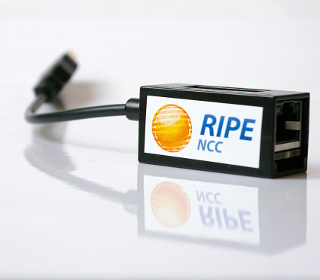
\includegraphics[width=.30\textwidth, height=.20\textwidth]{illustrations/v1} 	\captionsetup{justification=centering}\caption{Génération 1}}
	\hfill
	\parbox{.32\textwidth}{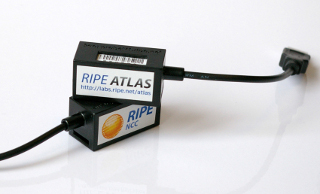
\includegraphics[width=.30\textwidth, height=.20\textwidth]{illustrations/v2}
		\captionsetup{justification=centering}
		\caption{Génération 2}}
	\hfill
	\parbox{.32\textwidth}{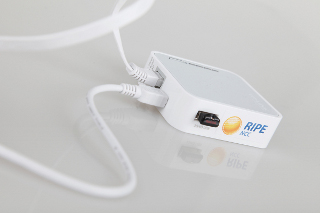
\includegraphics[width=.30\textwidth,height=.20\textwidth]{illustrations/v3} 	\captionsetup{justification=centering}\caption{Génération 3}}
	\caption{Les trois générations des sondes Atlas}
	\label{fig:genarations}
	\source{\url{https://atlas.ripe.net/docs/}, consultée le $05/08/2018$.}
\end{figure}

Pour précision, les générations $1$ et $2$ présentent une très faible consommation d'énergie, cependant, elles ont un temps de redémarrage et coûts de production élevés. 

%Pour la génération $3$, même si elle est conçue en utilisant tp-link tl-mr3020,  la sonde v3 ne sert pas comme un routeur Wi-Fi.
%, pourtant, elle a les mêmes fonctionnalités que les sondes v1 et v2.

En $2015$, plusieurs utilisateurs des sondes  Atlas ont montré un intérêt aux sondes virtuelles. Les sondes virtuelles présentent des avantages et aussi des inconvénients. Parmi les avantages, la conception des sondes virtuelles permet d'explorer des emplacements qui sont difficilement accessibles. En effet, cela permet d'étendre le réseau des sondes  Atlas. D'autre part, les sondes virtuelles peuvent être installées sans contraintes physiques ou organisationnelles. Parmi les inconvénients, une complexité sera ajoutée au système RIPE Atlas, plus de ressources seront demandées. De plus, il peut y avoir le problème de la qualité de données; le manque de données peut faire référence à une perte de paquets ou bien la machine qui héberge la sonde n'est plus disponible pour continuer les mesures. 


\subsection{Les versions du firmware des sondes Atlas} \label{subsec:firmwareversion}
En principe, toutes les sondes Atlas collectent la même information, indépendamment de leur version du firmware. On trouve les mêmes attributs\footnote{Attribut dans le sens du JSON : chaque résultat de mesure est enregistré comme étant un objet JSON.}  dans toutes les versions sauf de léger changements : ajout d'un ou de plusieurs attributs, la modification des noms des attributs, etc. Pour la simplification, nous donnons un identifiant entier pour chaque version, entre les parenthèses. Cet identifiant sera utilisé dans la suite de ce document. 

%Les résultats de mesures  sont sauvegardés dans des fichiers JSON. Chaque mesure est un tableau d'éléments. chaque élément est un tableau associative. La structure des tableau associatifs dépend de la version du firmware. \par


Il existe plusieurs versions du firmware:
\begin{itemize}
	\setlength\itemsep{0.1 cm}
	\item[--] version $1$ est identifié par  $1$ (1);
	\item[--] version $4400$  est identifiée par une valeur entre  $4400$ et $4459$ (2);
	\item[--] version $4460$ est identifiée par une valeur entre $4460$ et $4539$ (3);
	\item[--] version $4540$  est identifiée par une valeur entre  $4540$ et $4569$ (4);
	\item[--]  version $4570$  est identifiée par une valeur entre $4570$ et $4609$ (5);
	\item[--] la dernière version du firmeware \footnote{A la date de consultation $ 25/01/2018 $.} est $4610$ (6). 
\end{itemize}

\subsection{La connexion des sondes Atlas à Internet}

Les génération $1$ et $2$ des sondes  Atlas ont une interface Ethernet (RJ-45). La génération $3$ dispose techniquement des capacités Wi-Fi. Cependant, ces sondes ne sont pas suffisamment prêtes au niveau logiciel pour supporter le Wi-Fi.
% L'objectif était de garder l'indépendance des sondes Atlas du trafic de celui qui les héberge.

Une fois la sonde se connecte au port d'Ethernet, elle acquiert  une adresse IPv4, un résolveur DNS  en utilisant DHCP et la configuration IPv6 via \textit{Router Advertisement}. Ensuite, elle essaie de rejoindre l'infrastructure du RIPE Atlas. Pour ce faire, elle utilise le résolveur DNS et se connecte à l'infrastructure à travers SSH sur le port TCP de sortie $443$ comme il est illustré dans la Figure \ref{fig:ssh-atlas-probe}. L'architecture du système RIPE Atlas est détaillée dans la section \ref{subsec:archi-probes}.

\begin{figure}[H]
	\centering
	\captionsetup{justification=centering}
	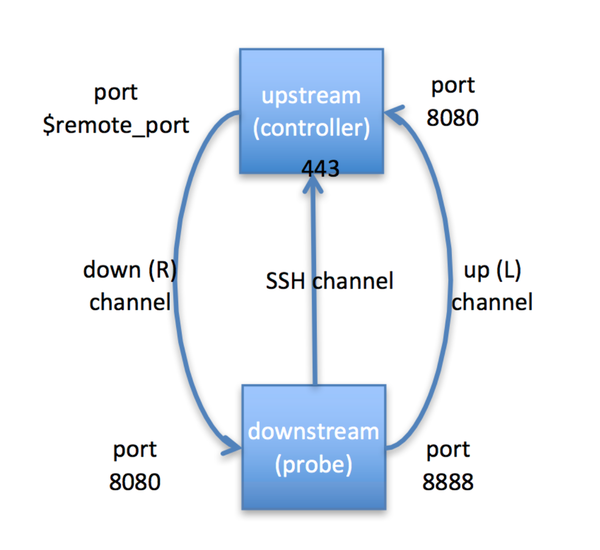
\includegraphics[width=0.5\linewidth]{illustrations/ssh-atlas-probe}
	\caption{La connexion des sondes Atlas à l'infrastructure RIPE Atlas \cite{how-we-manage-our-probe}}
	\label{fig:ssh-atlas-probe}
\end{figure}

\subsection{Architecture du système RIPE Atlas} \label{subsec:archi-probes}

Il existe deux catégories d'outils de surveillance du réseau: des outils matériels et d'autres logiciels. Les sondes  Atlas sont parmi les outils matériels. Le choix d'utilisation d'un outil matériel au lieu d'un outil logiciel dépend de plusieurs facteurs, par exemple l'indépendance du système d'exploitation, la facilité de déploiement, la disponibilité des sondes tout le temps (au lieu d'être dépendante de la machine qui l'héberge) et d'autres facteurs liés à la sécurité.

Le système RIPE Atlas est conçu pour qu'il soit opérationnel de façon distribuée. La plupart des composantes ont assez de connaissances pour remplir leurs rôles, sans nécessairement avoir besoin de connaître les états des autres composantes du système. Cela assure que le système soit capable d'assurer la plupart des fonctionnalités en cas  d'un problème temporaire. Par exemple, si une sonde est déconnectée de l'infrastructure, elle continue les mesures planifiées et les données sont renvoyées dès sa reconnexion au système.


La Figure  \ref{fig:archi-ripe-atlas} montre une vue d'ensemble de l'architecture du RIPE Atlas.

\begin{figure}[H]
	\centering
	\resizebox{\textwidth}{!}{
		% Graphic for TeX using PGF
% Title: /home/bellafkih/Documents/2017-2018/Mémoire/report_memoire/illustrations/Diagramme1.dia
% Creator: Dia v0.97.3
% CreationDate: Thu Mar  1 16:26:10 2018
% For: bellafkih
% \usepackage{tikz}
% The following commands are not supported in PSTricks at present
% We define them conditionally, so when they are implemented,
% this pgf file will use them.
\ifx\du\undefined
  \newlength{\du}
\fi
\setlength{\du}{15\unitlength}
\begin{tikzpicture}
\pgftransformxscale{1.000000}
\pgftransformyscale{-1.000000}
\definecolor{dialinecolor}{rgb}{0.000000, 0.000000, 0.000000}
\pgfsetstrokecolor{dialinecolor}
\definecolor{dialinecolor}{rgb}{1.000000, 1.000000, 1.000000}
\pgfsetfillcolor{dialinecolor}
\pgfsetlinewidth{0.100000\du}
\pgfsetdash{}{0pt}
\pgfsetdash{}{0pt}
\pgfsetbuttcap
\pgfsetmiterjoin
\pgfsetlinewidth{0.100000\du}
\pgfsetbuttcap
\pgfsetmiterjoin
\pgfsetdash{}{0pt}
\definecolor{dialinecolor}{rgb}{0.698039, 0.690196, 0.690196}
\pgfsetfillcolor{dialinecolor}
\pgfpathmoveto{\pgfpoint{16.900000\du}{2.091667\du}}
\pgfpathcurveto{\pgfpoint{17.870000\du}{1.610417\du}}{\pgfpoint{18.355000\du}{1.450000\du}}{\pgfpoint{19.325000\du}{1.450000\du}}
\pgfpathcurveto{\pgfpoint{20.295000\du}{1.450000\du}}{\pgfpoint{20.780000\du}{1.610417\du}}{\pgfpoint{21.750000\du}{2.091667\du}}
\pgfpathlineto{\pgfpoint{21.750000\du}{4.658333\du}}
\pgfpathcurveto{\pgfpoint{20.780000\du}{5.139583\du}}{\pgfpoint{20.295000\du}{5.300000\du}}{\pgfpoint{19.325000\du}{5.300000\du}}
\pgfpathcurveto{\pgfpoint{18.355000\du}{5.300000\du}}{\pgfpoint{17.870000\du}{5.139583\du}}{\pgfpoint{16.900000\du}{4.658333\du}}
\pgfpathlineto{\pgfpoint{16.900000\du}{2.091667\du}}
\pgfusepath{fill}
\definecolor{dialinecolor}{rgb}{0.000000, 0.000000, 0.000000}
\pgfsetstrokecolor{dialinecolor}
\pgfpathmoveto{\pgfpoint{16.900000\du}{2.091667\du}}
\pgfpathcurveto{\pgfpoint{17.870000\du}{1.610417\du}}{\pgfpoint{18.355000\du}{1.450000\du}}{\pgfpoint{19.325000\du}{1.450000\du}}
\pgfpathcurveto{\pgfpoint{20.295000\du}{1.450000\du}}{\pgfpoint{20.780000\du}{1.610417\du}}{\pgfpoint{21.750000\du}{2.091667\du}}
\pgfpathlineto{\pgfpoint{21.750000\du}{4.658333\du}}
\pgfpathcurveto{\pgfpoint{20.780000\du}{5.139583\du}}{\pgfpoint{20.295000\du}{5.300000\du}}{\pgfpoint{19.325000\du}{5.300000\du}}
\pgfpathcurveto{\pgfpoint{18.355000\du}{5.300000\du}}{\pgfpoint{17.870000\du}{5.139583\du}}{\pgfpoint{16.900000\du}{4.658333\du}}
\pgfpathlineto{\pgfpoint{16.900000\du}{2.091667\du}}
\pgfusepath{stroke}
\pgfsetbuttcap
\pgfsetmiterjoin
\pgfsetdash{}{0pt}
\definecolor{dialinecolor}{rgb}{0.000000, 0.000000, 0.000000}
\pgfsetstrokecolor{dialinecolor}
\pgfpathmoveto{\pgfpoint{16.900000\du}{2.091667\du}}
\pgfpathcurveto{\pgfpoint{17.870000\du}{2.572917\du}}{\pgfpoint{18.355000\du}{2.733333\du}}{\pgfpoint{19.325000\du}{2.733333\du}}
\pgfpathcurveto{\pgfpoint{20.295000\du}{2.733333\du}}{\pgfpoint{20.780000\du}{2.572917\du}}{\pgfpoint{21.750000\du}{2.091667\du}}
\pgfusepath{stroke}
% setfont left to latex
\definecolor{dialinecolor}{rgb}{0.000000, 0.000000, 0.000000}
\pgfsetstrokecolor{dialinecolor}
\node at (19.325000\du,3.895833\du){DB};
\definecolor{dialinecolor}{rgb}{0.682353, 0.627451, 0.627451}
\pgfsetfillcolor{dialinecolor}
\fill (10.950000\du,4.100000\du)--(10.950000\du,6.400000\du)--(13.350000\du,6.400000\du)--(13.350000\du,4.100000\du)--cycle;
\pgfsetlinewidth{0.100000\du}
\pgfsetdash{}{0pt}
\pgfsetdash{}{0pt}
\pgfsetmiterjoin
\definecolor{dialinecolor}{rgb}{0.000000, 0.000000, 0.000000}
\pgfsetstrokecolor{dialinecolor}
\draw (10.950000\du,4.100000\du)--(10.950000\du,6.400000\du)--(13.350000\du,6.400000\du)--(13.350000\du,4.100000\du)--cycle;
% setfont left to latex
\definecolor{dialinecolor}{rgb}{0.000000, 0.000000, 0.000000}
\pgfsetstrokecolor{dialinecolor}
\node at (12.150000\du,5.445000\du){UI};
\definecolor{dialinecolor}{rgb}{0.898039, 0.898039, 0.898039}
\pgfsetfillcolor{dialinecolor}
\fill (17.586250\du,6.675000\du)--(17.586250\du,9.350000\du)--(21.750000\du,9.350000\du)--(21.750000\du,6.675000\du)--cycle;
\pgfsetlinewidth{0.050000\du}
\pgfsetdash{}{0pt}
\pgfsetdash{}{0pt}
\pgfsetmiterjoin
\definecolor{dialinecolor}{rgb}{0.000000, 0.000000, 0.000000}
\pgfsetstrokecolor{dialinecolor}
\draw (17.586250\du,6.675000\du)--(17.586250\du,9.350000\du)--(21.750000\du,9.350000\du)--(21.750000\du,6.675000\du)--cycle;
% setfont left to latex
\definecolor{dialinecolor}{rgb}{0.000000, 0.000000, 0.000000}
\pgfsetstrokecolor{dialinecolor}
\node at (19.668125\du,8.207500\du){};
\definecolor{dialinecolor}{rgb}{0.898039, 0.898039, 0.898039}
\pgfsetfillcolor{dialinecolor}
\fill (17.310000\du,6.405000\du)--(17.310000\du,9.080000\du)--(21.473750\du,9.080000\du)--(21.473750\du,6.405000\du)--cycle;
\pgfsetlinewidth{0.050000\du}
\pgfsetdash{}{0pt}
\pgfsetdash{}{0pt}
\pgfsetmiterjoin
\definecolor{dialinecolor}{rgb}{0.000000, 0.000000, 0.000000}
\pgfsetstrokecolor{dialinecolor}
\draw (17.310000\du,6.405000\du)--(17.310000\du,9.080000\du)--(21.473750\du,9.080000\du)--(21.473750\du,6.405000\du)--cycle;
% setfont left to latex
\definecolor{dialinecolor}{rgb}{0.000000, 0.000000, 0.000000}
\pgfsetstrokecolor{dialinecolor}
\node at (19.391875\du,7.937500\du){};
\definecolor{dialinecolor}{rgb}{0.498039, 0.498039, 0.498039}
\pgfsetfillcolor{dialinecolor}
\fill (25.385000\du,5.955000\du)--(25.385000\du,8.830000\du)--(29.885000\du,8.830000\du)--(29.885000\du,5.955000\du)--cycle;
\pgfsetlinewidth{0.050000\du}
\pgfsetdash{}{0pt}
\pgfsetdash{}{0pt}
\pgfsetmiterjoin
\definecolor{dialinecolor}{rgb}{0.000000, 0.000000, 0.000000}
\pgfsetstrokecolor{dialinecolor}
\draw (25.385000\du,5.955000\du)--(25.385000\du,8.830000\du)--(29.885000\du,8.830000\du)--(29.885000\du,5.955000\du)--cycle;
% setfont left to latex
\definecolor{dialinecolor}{rgb}{0.000000, 0.000000, 0.000000}
\pgfsetstrokecolor{dialinecolor}
\node at (27.635000\du,7.587500\du){};
\definecolor{dialinecolor}{rgb}{0.498039, 0.498039, 0.498039}
\pgfsetfillcolor{dialinecolor}
\fill (25.760000\du,6.255000\du)--(25.760000\du,9.130000\du)--(30.260000\du,9.130000\du)--(30.260000\du,6.255000\du)--cycle;
\pgfsetlinewidth{0.050000\du}
\pgfsetdash{}{0pt}
\pgfsetdash{}{0pt}
\pgfsetmiterjoin
\definecolor{dialinecolor}{rgb}{0.000000, 0.000000, 0.000000}
\pgfsetstrokecolor{dialinecolor}
\draw (25.760000\du,6.255000\du)--(25.760000\du,9.130000\du)--(30.260000\du,9.130000\du)--(30.260000\du,6.255000\du)--cycle;
% setfont left to latex
\definecolor{dialinecolor}{rgb}{0.000000, 0.000000, 0.000000}
\pgfsetstrokecolor{dialinecolor}
\node at (28.010000\du,7.887500\du){};
\definecolor{dialinecolor}{rgb}{0.847059, 0.898039, 0.898039}
\pgfsetfillcolor{dialinecolor}
\fill (18.300000\du,11.900000\du)--(18.300000\du,15.025000\du)--(21.850000\du,15.025000\du)--(21.850000\du,11.900000\du)--cycle;
\pgfsetlinewidth{0.050000\du}
\pgfsetdash{}{0pt}
\pgfsetdash{}{0pt}
\pgfsetmiterjoin
\definecolor{dialinecolor}{rgb}{0.000000, 0.000000, 0.000000}
\pgfsetstrokecolor{dialinecolor}
\draw (18.300000\du,11.900000\du)--(18.300000\du,15.025000\du)--(21.850000\du,15.025000\du)--(21.850000\du,11.900000\du)--cycle;
% setfont left to latex
\definecolor{dialinecolor}{rgb}{0.000000, 0.000000, 0.000000}
\pgfsetstrokecolor{dialinecolor}
\node at (20.075000\du,13.657500\du){};
\definecolor{dialinecolor}{rgb}{0.847059, 0.898039, 0.898039}
\pgfsetfillcolor{dialinecolor}
\fill (17.960000\du,11.455000\du)--(17.960000\du,14.580000\du)--(21.510000\du,14.580000\du)--(21.510000\du,11.455000\du)--cycle;
\pgfsetlinewidth{0.050000\du}
\pgfsetdash{}{0pt}
\pgfsetdash{}{0pt}
\pgfsetmiterjoin
\definecolor{dialinecolor}{rgb}{0.000000, 0.000000, 0.000000}
\pgfsetstrokecolor{dialinecolor}
\draw (17.960000\du,11.455000\du)--(17.960000\du,14.580000\du)--(21.510000\du,14.580000\du)--(21.510000\du,11.455000\du)--cycle;
% setfont left to latex
\definecolor{dialinecolor}{rgb}{0.000000, 0.000000, 0.000000}
\pgfsetstrokecolor{dialinecolor}
\node at (19.735000\du,13.212500\du){};
\pgfsetlinewidth{0.050000\du}
\pgfsetdash{}{0pt}
\pgfsetdash{}{0pt}
\pgfsetbuttcap
\pgfsetmiterjoin
\pgfsetlinewidth{0.050000\du}
\pgfsetbuttcap
\pgfsetmiterjoin
\pgfsetdash{}{0pt}
\definecolor{dialinecolor}{rgb}{0.854902, 0.788235, 0.854902}
\pgfsetfillcolor{dialinecolor}
\pgfpathmoveto{\pgfpoint{7.085270\du}{11.834673\du}}
\pgfpathcurveto{\pgfpoint{6.451876\du}{11.817409\du}}{\pgfpoint{5.223477\du}{12.179945\du}}{\pgfpoint{5.396221\du}{12.956808\du}}
\pgfpathcurveto{\pgfpoint{5.568963\du}{13.733671\du}}{\pgfpoint{6.394295\du}{13.906300\du}}{\pgfpoint{6.739782\du}{13.681880\du}}
\pgfpathcurveto{\pgfpoint{7.085270\du}{13.457453\du}}{\pgfpoint{6.202357\du}{14.769481\du}}{\pgfpoint{7.891408\du}{15.114754\du}}
\pgfpathcurveto{\pgfpoint{9.580443\du}{15.460026\du}}{\pgfpoint{10.444162\du}{14.907590\du}}{\pgfpoint{10.194643\du}{14.510527\du}}
\pgfpathcurveto{\pgfpoint{9.945124\du}{14.113464\du}}{\pgfpoint{11.672562\du}{15.442763\du}}{\pgfpoint{12.478700\du}{14.683163\du}}
\pgfpathcurveto{\pgfpoint{13.284837\du}{13.923564\du}}{\pgfpoint{11.653368\du}{13.198499\du}}{\pgfpoint{11.998856\du}{13.302081\du}}
\pgfpathcurveto{\pgfpoint{12.344343\du}{13.405662\du}}{\pgfpoint{13.400000\du}{13.267553\du}}{\pgfpoint{13.054512\du}{11.972782\du}}
\pgfpathcurveto{\pgfpoint{12.709025\du}{10.678010\du}}{\pgfpoint{9.599636\du}{11.679300\du}}{\pgfpoint{9.945124\du}{11.489401\du}}
\pgfpathcurveto{\pgfpoint{10.290612\du}{11.299501\du}}{\pgfpoint{9.426893\du}{10.350000\du}}{\pgfpoint{8.352058\du}{10.539900\du}}
\pgfpathcurveto{\pgfpoint{7.277207\du}{10.729801\du}}{\pgfpoint{7.200970\du}{11.074400\du}}{\pgfpoint{7.085807\du}{11.834000\du}}
\pgfpathlineto{\pgfpoint{7.085270\du}{11.834673\du}}
\pgfusepath{fill}
\definecolor{dialinecolor}{rgb}{0.000000, 0.000000, 0.000000}
\pgfsetstrokecolor{dialinecolor}
\pgfpathmoveto{\pgfpoint{7.085270\du}{11.834673\du}}
\pgfpathcurveto{\pgfpoint{6.451876\du}{11.817409\du}}{\pgfpoint{5.223477\du}{12.179945\du}}{\pgfpoint{5.396221\du}{12.956808\du}}
\pgfpathcurveto{\pgfpoint{5.568963\du}{13.733671\du}}{\pgfpoint{6.394295\du}{13.906300\du}}{\pgfpoint{6.739782\du}{13.681880\du}}
\pgfpathcurveto{\pgfpoint{7.085270\du}{13.457453\du}}{\pgfpoint{6.202357\du}{14.769481\du}}{\pgfpoint{7.891408\du}{15.114754\du}}
\pgfpathcurveto{\pgfpoint{9.580443\du}{15.460026\du}}{\pgfpoint{10.444162\du}{14.907590\du}}{\pgfpoint{10.194643\du}{14.510527\du}}
\pgfpathcurveto{\pgfpoint{9.945124\du}{14.113464\du}}{\pgfpoint{11.672562\du}{15.442763\du}}{\pgfpoint{12.478700\du}{14.683163\du}}
\pgfpathcurveto{\pgfpoint{13.284837\du}{13.923564\du}}{\pgfpoint{11.653368\du}{13.198499\du}}{\pgfpoint{11.998856\du}{13.302081\du}}
\pgfpathcurveto{\pgfpoint{12.344343\du}{13.405662\du}}{\pgfpoint{13.400000\du}{13.267553\du}}{\pgfpoint{13.054512\du}{11.972782\du}}
\pgfpathcurveto{\pgfpoint{12.709025\du}{10.678010\du}}{\pgfpoint{9.599636\du}{11.679300\du}}{\pgfpoint{9.945124\du}{11.489401\du}}
\pgfpathcurveto{\pgfpoint{10.290612\du}{11.299501\du}}{\pgfpoint{9.426893\du}{10.350000\du}}{\pgfpoint{8.352058\du}{10.539900\du}}
\pgfpathcurveto{\pgfpoint{7.277207\du}{10.729801\du}}{\pgfpoint{7.200970\du}{11.074400\du}}{\pgfpoint{7.085807\du}{11.834000\du}}
\pgfpathlineto{\pgfpoint{7.085270\du}{11.834673\du}}
\pgfusepath{stroke}
% setfont left to latex
\definecolor{dialinecolor}{rgb}{0.000000, 0.000000, 0.000000}
\pgfsetstrokecolor{dialinecolor}
\node at (9.530923\du,13.195092\du){Data Storage};
\definecolor{dialinecolor}{rgb}{0.380392, 0.549020, 0.603922}
\pgfsetfillcolor{dialinecolor}
\fill (22.111250\du,16.630000\du)--(22.111250\du,19.305000\du)--(26.700000\du,19.305000\du)--(26.700000\du,16.630000\du)--cycle;
\pgfsetlinewidth{0.050000\du}
\pgfsetdash{}{0pt}
\pgfsetdash{}{0pt}
\pgfsetmiterjoin
\definecolor{dialinecolor}{rgb}{0.000000, 0.000000, 0.000000}
\pgfsetstrokecolor{dialinecolor}
\draw (22.111250\du,16.630000\du)--(22.111250\du,19.305000\du)--(26.700000\du,19.305000\du)--(26.700000\du,16.630000\du)--cycle;
% setfont left to latex
\definecolor{dialinecolor}{rgb}{0.000000, 0.000000, 0.000000}
\pgfsetstrokecolor{dialinecolor}
\node at (24.405625\du,18.162500\du){Controller};
\definecolor{dialinecolor}{rgb}{0.380392, 0.549020, 0.603922}
\pgfsetfillcolor{dialinecolor}
\fill (13.760000\du,16.630000\du)--(13.760000\du,19.305000\du)--(18.348750\du,19.305000\du)--(18.348750\du,16.630000\du)--cycle;
\pgfsetlinewidth{0.050000\du}
\pgfsetdash{}{0pt}
\pgfsetdash{}{0pt}
\pgfsetmiterjoin
\definecolor{dialinecolor}{rgb}{0.000000, 0.000000, 0.000000}
\pgfsetstrokecolor{dialinecolor}
\draw (13.760000\du,16.630000\du)--(13.760000\du,19.305000\du)--(18.348750\du,19.305000\du)--(18.348750\du,16.630000\du)--cycle;
% setfont left to latex
\definecolor{dialinecolor}{rgb}{0.000000, 0.000000, 0.000000}
\pgfsetstrokecolor{dialinecolor}
\node at (16.054375\du,18.162500\du){Controller};
\definecolor{dialinecolor}{rgb}{0.996078, 0.960784, 1.000000}
\pgfsetfillcolor{dialinecolor}
\fill (12.471250\du,21.075000\du)--(12.471250\du,22.925000\du)--(15.528750\du,22.925000\du)--(15.528750\du,21.075000\du)--cycle;
\pgfsetlinewidth{0.050000\du}
\pgfsetdash{}{0pt}
\pgfsetdash{}{0pt}
\pgfsetmiterjoin
\definecolor{dialinecolor}{rgb}{0.000000, 0.000000, 0.000000}
\pgfsetstrokecolor{dialinecolor}
\draw (12.471250\du,21.075000\du)--(12.471250\du,22.925000\du)--(15.528750\du,22.925000\du)--(15.528750\du,21.075000\du)--cycle;
% setfont left to latex
\definecolor{dialinecolor}{rgb}{0.000000, 0.000000, 0.000000}
\pgfsetstrokecolor{dialinecolor}
\node at (14.000000\du,22.195000\du){Sonde};
\definecolor{dialinecolor}{rgb}{0.996078, 0.960784, 1.000000}
\pgfsetfillcolor{dialinecolor}
\fill (17.360000\du,21.080000\du)--(17.360000\du,22.930000\du)--(20.417500\du,22.930000\du)--(20.417500\du,21.080000\du)--cycle;
\pgfsetlinewidth{0.050000\du}
\pgfsetdash{}{0pt}
\pgfsetdash{}{0pt}
\pgfsetmiterjoin
\definecolor{dialinecolor}{rgb}{0.000000, 0.000000, 0.000000}
\pgfsetstrokecolor{dialinecolor}
\draw (17.360000\du,21.080000\du)--(17.360000\du,22.930000\du)--(20.417500\du,22.930000\du)--(20.417500\du,21.080000\du)--cycle;
% setfont left to latex
\definecolor{dialinecolor}{rgb}{0.000000, 0.000000, 0.000000}
\pgfsetstrokecolor{dialinecolor}
\node at (18.888750\du,22.200000\du){Sonde};
\definecolor{dialinecolor}{rgb}{0.996078, 0.960784, 1.000000}
\pgfsetfillcolor{dialinecolor}
\fill (20.845000\du,21.035000\du)--(20.845000\du,22.885000\du)--(23.902500\du,22.885000\du)--(23.902500\du,21.035000\du)--cycle;
\pgfsetlinewidth{0.050000\du}
\pgfsetdash{}{0pt}
\pgfsetdash{}{0pt}
\pgfsetmiterjoin
\definecolor{dialinecolor}{rgb}{0.000000, 0.000000, 0.000000}
\pgfsetstrokecolor{dialinecolor}
\draw (20.845000\du,21.035000\du)--(20.845000\du,22.885000\du)--(23.902500\du,22.885000\du)--(23.902500\du,21.035000\du)--cycle;
% setfont left to latex
\definecolor{dialinecolor}{rgb}{0.000000, 0.000000, 0.000000}
\pgfsetstrokecolor{dialinecolor}
\node at (22.373750\du,22.155000\du){Sonde};
\definecolor{dialinecolor}{rgb}{0.996078, 0.960784, 1.000000}
\pgfsetfillcolor{dialinecolor}
\fill (25.680000\du,20.990000\du)--(25.680000\du,22.840000\du)--(28.737500\du,22.840000\du)--(28.737500\du,20.990000\du)--cycle;
\pgfsetlinewidth{0.050000\du}
\pgfsetdash{}{0pt}
\pgfsetdash{}{0pt}
\pgfsetmiterjoin
\definecolor{dialinecolor}{rgb}{0.000000, 0.000000, 0.000000}
\pgfsetstrokecolor{dialinecolor}
\draw (25.680000\du,20.990000\du)--(25.680000\du,22.840000\du)--(28.737500\du,22.840000\du)--(28.737500\du,20.990000\du)--cycle;
% setfont left to latex
\definecolor{dialinecolor}{rgb}{0.000000, 0.000000, 0.000000}
\pgfsetstrokecolor{dialinecolor}
\node at (27.208750\du,22.110000\du){Sonde};
% setfont left to latex
\definecolor{dialinecolor}{rgb}{0.000000, 0.000000, 0.000000}
\pgfsetstrokecolor{dialinecolor}
\node[anchor=west] at (26.350000\du,7.750000\du){Reg.server};
\pgfsetlinewidth{0.050000\du}
\pgfsetdash{}{0pt}
\pgfsetdash{}{0pt}
\pgfsetbuttcap
{
\definecolor{dialinecolor}{rgb}{0.000000, 0.000000, 0.000000}
\pgfsetfillcolor{dialinecolor}
% was here!!!
\definecolor{dialinecolor}{rgb}{0.000000, 0.000000, 0.000000}
\pgfsetstrokecolor{dialinecolor}
\draw (21.750000\du,3.054167\du)--(25.385000\du,7.392500\du);
}
\pgfsetlinewidth{0.050000\du}
\pgfsetdash{}{0pt}
\pgfsetdash{}{0pt}
\pgfsetbuttcap
{
\definecolor{dialinecolor}{rgb}{0.000000, 0.000000, 0.000000}
\pgfsetfillcolor{dialinecolor}
% was here!!!
\definecolor{dialinecolor}{rgb}{0.000000, 0.000000, 0.000000}
\pgfsetstrokecolor{dialinecolor}
\draw (13.350000\du,5.250000\du)--(16.900000\du,3.054167\du);
}
% setfont left to latex
\definecolor{dialinecolor}{rgb}{0.000000, 0.000000, 0.000000}
\pgfsetstrokecolor{dialinecolor}
\node[anchor=west] at (18.600000\du,7.900000\du){Brain};
\pgfsetlinewidth{0.050000\du}
\pgfsetdash{}{0pt}
\pgfsetdash{}{0pt}
\pgfsetbuttcap
{
\definecolor{dialinecolor}{rgb}{0.000000, 0.000000, 0.000000}
\pgfsetfillcolor{dialinecolor}
% was here!!!
\definecolor{dialinecolor}{rgb}{0.000000, 0.000000, 0.000000}
\pgfsetstrokecolor{dialinecolor}
\draw (19.325000\du,5.300000\du)--(19.354568\du,6.379924\du);
}
% setfont left to latex
\definecolor{dialinecolor}{rgb}{0.000000, 0.000000, 0.000000}
\pgfsetstrokecolor{dialinecolor}
\node[anchor=west] at (19.150000\du,13.300000\du){MQ};
\pgfsetlinewidth{0.050000\du}
\pgfsetdash{}{0pt}
\pgfsetdash{}{0pt}
\pgfsetbuttcap
{
\definecolor{dialinecolor}{rgb}{0.000000, 0.000000, 0.000000}
\pgfsetfillcolor{dialinecolor}
% was here!!!
\definecolor{dialinecolor}{rgb}{0.000000, 0.000000, 0.000000}
\pgfsetstrokecolor{dialinecolor}
\draw (19.668125\du,9.350000\du)--(19.735000\du,11.455000\du);
}
\pgfsetlinewidth{0.050000\du}
\pgfsetdash{}{0pt}
\pgfsetdash{}{0pt}
\pgfsetbuttcap
{
\definecolor{dialinecolor}{rgb}{0.000000, 0.000000, 0.000000}
\pgfsetfillcolor{dialinecolor}
% was here!!!
\definecolor{dialinecolor}{rgb}{0.000000, 0.000000, 0.000000}
\pgfsetstrokecolor{dialinecolor}
\draw (10.026768\du,11.262769\du)--(12.150000\du,6.400000\du);
}
\pgfsetlinewidth{0.050000\du}
\pgfsetdash{}{0pt}
\pgfsetdash{}{0pt}
\pgfsetbuttcap
{
\definecolor{dialinecolor}{rgb}{0.000000, 0.000000, 0.000000}
\pgfsetfillcolor{dialinecolor}
% was here!!!
\definecolor{dialinecolor}{rgb}{0.000000, 0.000000, 0.000000}
\pgfsetstrokecolor{dialinecolor}
\draw (13.015462\du,12.942453\du)--(17.960000\du,13.017500\du);
}
\pgfsetlinewidth{0.050000\du}
\pgfsetdash{}{0pt}
\pgfsetdash{}{0pt}
\pgfsetbuttcap
{
\definecolor{dialinecolor}{rgb}{0.000000, 0.000000, 0.000000}
\pgfsetfillcolor{dialinecolor}
% was here!!!
\definecolor{dialinecolor}{rgb}{0.000000, 0.000000, 0.000000}
\pgfsetstrokecolor{dialinecolor}
\draw (20.075000\du,15.025000\du)--(24.405625\du,16.630000\du);
}
\pgfsetlinewidth{0.050000\du}
\pgfsetdash{}{0pt}
\pgfsetdash{}{0pt}
\pgfsetbuttcap
{
\definecolor{dialinecolor}{rgb}{0.000000, 0.000000, 0.000000}
\pgfsetfillcolor{dialinecolor}
% was here!!!
\definecolor{dialinecolor}{rgb}{0.000000, 0.000000, 0.000000}
\pgfsetstrokecolor{dialinecolor}
\draw (20.075000\du,15.025000\du)--(16.054375\du,16.630000\du);
}
\pgfsetlinewidth{0.050000\du}
\pgfsetdash{}{0pt}
\pgfsetdash{}{0pt}
\pgfsetbuttcap
{
\definecolor{dialinecolor}{rgb}{0.000000, 0.000000, 0.000000}
\pgfsetfillcolor{dialinecolor}
% was here!!!
\definecolor{dialinecolor}{rgb}{0.000000, 0.000000, 0.000000}
\pgfsetstrokecolor{dialinecolor}
\draw (14.907187\du,19.305000\du)--(14.000000\du,21.075000\du);
}
\pgfsetlinewidth{0.050000\du}
\pgfsetdash{}{0pt}
\pgfsetdash{}{0pt}
\pgfsetbuttcap
{
\definecolor{dialinecolor}{rgb}{0.000000, 0.000000, 0.000000}
\pgfsetfillcolor{dialinecolor}
% was here!!!
\definecolor{dialinecolor}{rgb}{0.000000, 0.000000, 0.000000}
\pgfsetstrokecolor{dialinecolor}
\draw (17.201562\du,19.305000\du)--(18.295186\du,21.055122\du);
}
\pgfsetlinewidth{0.050000\du}
\pgfsetdash{}{0pt}
\pgfsetdash{}{0pt}
\pgfsetbuttcap
{
\definecolor{dialinecolor}{rgb}{0.000000, 0.000000, 0.000000}
\pgfsetfillcolor{dialinecolor}
% was here!!!
\definecolor{dialinecolor}{rgb}{0.000000, 0.000000, 0.000000}
\pgfsetstrokecolor{dialinecolor}
\draw (23.503782\du,19.329003\du)--(22.373750\du,21.035000\du);
}
\pgfsetlinewidth{0.050000\du}
\pgfsetdash{}{0pt}
\pgfsetdash{}{0pt}
\pgfsetbuttcap
{
\definecolor{dialinecolor}{rgb}{0.000000, 0.000000, 0.000000}
\pgfsetfillcolor{dialinecolor}
% was here!!!
\definecolor{dialinecolor}{rgb}{0.000000, 0.000000, 0.000000}
\pgfsetstrokecolor{dialinecolor}
\draw (25.552813\du,19.305000\du)--(27.208750\du,20.990000\du);
}
\pgfsetlinewidth{0.100000\du}
\pgfsetdash{{\pgflinewidth}{0.200000\du}}{0cm}
\pgfsetdash{{\pgflinewidth}{0.200000\du}}{0cm}
\pgfsetbuttcap
{
\definecolor{dialinecolor}{rgb}{0.000000, 0.000000, 0.000000}
\pgfsetfillcolor{dialinecolor}
% was here!!!
\pgfsetarrowsend{stealth}
\definecolor{dialinecolor}{rgb}{0.000000, 0.000000, 0.000000}
\pgfsetstrokecolor{dialinecolor}
\pgfpathmoveto{\pgfpoint{28.736844\du}{21.915314\du}}
\pgfpatharc{65}{-52}{8.407488\du and 8.407488\du}
\pgfusepath{stroke}
}
\pgfsetlinewidth{0.050000\du}
\pgfsetdash{}{0pt}
\pgfsetdash{}{0pt}
\pgfsetbuttcap
{
\definecolor{dialinecolor}{rgb}{0.000000, 0.000000, 0.000000}
\pgfsetfillcolor{dialinecolor}
% was here!!!
\definecolor{dialinecolor}{rgb}{0.000000, 0.000000, 0.000000}
\pgfsetstrokecolor{dialinecolor}
\draw (25.385000\du,7.392500\du)--(19.735000\du,11.455000\du);
}
\pgfsetlinewidth{0.050000\du}
\pgfsetdash{}{0pt}
\pgfsetdash{}{0pt}
\pgfsetbuttcap
{
\definecolor{dialinecolor}{rgb}{0.000000, 0.000000, 0.000000}
\pgfsetfillcolor{dialinecolor}
% was here!!!
\definecolor{dialinecolor}{rgb}{0.000000, 0.000000, 0.000000}
\pgfsetstrokecolor{dialinecolor}
\draw (13.350000\du,6.400000\du)--(19.735000\du,11.455000\du);
}
\end{tikzpicture}
 
	}
	\caption{L'architecture du système  RIPE Atlas  }
	\source{Schéma repris du travail de Kisteleki \cite{WinNT}}
	\label{fig:archi-ripe-atlas}
\end{figure}

L'architecture du système  RIPE Atlas est constituée par  les composantes suivantes:
\begin{description}
	\item [Registration server] (Reg.server) : c'est le seul point d'entrée de confiance pour les sondes Atlas. Son rôle est de recevoir toutes les sondes désirant se connecter au système RIPE Atlas. Ensuite, il redirige chaque sonde vers le contrôleur adéquat, qui est le plus proche de la sonde et que est  suffisamment non occupé.  Le serveur d'enregistrement  a un aperçu de haut niveau du système.
	
	\item [Controller]: un contrôleur accepte d'établir une connexion avec une sonde parmi celles dont il a reçu leurs clés du serveur d'enregistrement (Reg.server). Une fois la connexion est établie entre une sonde et un contrôleur, ce dernier garde cette connexion active pour recevoir les résultats et prévenir la sonde des mesures à effectuer.  Le rôle du contrôleur est de communiquer avec les sondes,  associer les mesures aux sondes en se basant sur la disponibilité de la sonde et sur autres critères, et enfin, collecter les résultats intermédiaires des mesures.
	
	\item [Message Queue (MQ)] : Tout d'abord définissons MQ:
	
	\begin{tcolorbox}[title=Message Queue]
		\og    \textbf{\textit{Message Queue ou file d'attente de message}} \textit{:  est une technique de programmation utilisée pour la communication interprocessus ou la communication de serveur-à-serveur. Les files d'attente de message permettent le fonctionnement des liaisons asynchrones normalisées entre deux serveurs, c'est-à-dire de canaux de communications tels que l'expéditeur et le récepteur du message ne sont pas contraints de s'attendre l'un l'autre, mais poursuivent chacun l'exécution de leurs tâches} \footnote{Source : \url{https://fr.wikipedia.org/wiki/File\_d'attente\_de\_message}, consultée le $05/08/2018$.}. \fg{}
	\end{tcolorbox} 
	
	Un cluster de serveurs MQ  agit comme un système nerveux central au sein de l'architecture du RIPE Atlas. Il gère la connectivité entre les composantes de l'infrastructure et  assure l'échange de messages avec un délai minimal. C'est cette composante qui élimine le besoin que les autres composantes de l'infrastructure soient au courant des états des autres composantes de l'infrastructure. En plus, chaque composante peut être ajoutée ou retirée sans devoir synchroniser cette information avec l'infrastructure entière. Si c'est le cas d'une déconnexion d'une composante, les messages seront sauvegardés sur différents niveaux jusqu'au moment de la reconnexion.
	
	
	
	\item [UI] (User Interface): elle s'occupe des interactions de l'utilisateur. Elle sert les pages pour l'interface graphique de mesures \cite{create-UDM}. Elle traite les appels en provenance de l'API \footnote{Source : \url{https://atlas.ripe.net/docs/api/v2/manual/}, consultée le $05/08/2018$.} et sert les demandes de téléchargement en provenance de l'API.
	
	\item [Brain] : il effectue des tâches de haut niveau dans le système, notamment la planification des mesures. Cette planification est basée sur les demandes reçues via l'interface graphique web de mesures (UI) ou bien via l'API. La planification passe par la  présélection des sondes Atlas et la négociation avec les contrôleurs pour voir la disponibilité des sondes Atlas. 
	
	
	\item [DB] : c'est une base de données SQL contenant toutes les informations du système RIPE Atlas : les informations sur les sondes et leurs propriétés, les meta-data des mesures, les utilisateurs, les crédits, etc. 
	
	\item [Data Storage] : c'est un cluster Hadoop/HBase pour le stockage à long terme de tous les résultats. Cette technologie permet aussi d'effectuer des calculs d'agrégation périodiques et  d'autres tâches. 
	
	
	\begin{tcolorbox}
		\textbf{\textit{Hadoop MapReduce}} est un modèle de programmation qui permet de traiter les données massives suivant une architecture distribuée dans un cluster.
		
		\textbf{\textit{HBase}} est une base de données non relationnelle et distribuée. Elle est adaptée au stockage de données massives.
	\end{tcolorbox} 
	
\end{description}


La Figure \ref{fig:deroulement-connexion-ripe-atlas} illustre les étapes d'établissement de la connexion entre une sonde Atlas  et  l'infrastructure RIPE Atlas.

\begin{figure}[H]
	\captionsetup{justification=centering}
	\centering
	\resizebox{\textwidth}{!}{
		% Graphic for TeX using PGF
% Title: /home/hayat/Desktop/RipeAtlasTraceroutesAnalysis/report/illustrations/dia/deroulement-connexion-ripe-atlas.dia
% Creator: Dia v0.97+git
% CreationDate: Thu Dec 27 13:35:47 2018
% For: hayat
% \usepackage{tikz}
% The following commands are not supported in PSTricks at present
% We define them conditionally, so when they are implemented,
% this pgf file will use them.
\ifx\du\undefined
  \newlength{\du}
\fi
\setlength{\du}{15\unitlength}
\begin{tikzpicture}[even odd rule]
\pgftransformxscale{1.000000}
\pgftransformyscale{-1.000000}
\definecolor{dialinecolor}{rgb}{0.000000, 0.000000, 0.000000}
\pgfsetstrokecolor{dialinecolor}
\pgfsetstrokeopacity{1.000000}
\definecolor{diafillcolor}{rgb}{1.000000, 1.000000, 1.000000}
\pgfsetfillcolor{diafillcolor}
\pgfsetfillopacity{1.000000}
\pgfsetlinewidth{0.050000\du}
\pgfsetdash{}{0pt}
\pgfsetbuttcap
\pgfsetmiterjoin
\pgfsetlinewidth{0.050000\du}
\pgfsetbuttcap
\pgfsetmiterjoin
\pgfsetdash{}{0pt}
\definecolor{diafillcolor}{rgb}{1.000000, 1.000000, 1.000000}
\pgfsetfillcolor{diafillcolor}
\pgfsetfillopacity{1.000000}
\definecolor{dialinecolor}{rgb}{0.890196, 0.835294, 0.835294}
\pgfsetstrokecolor{dialinecolor}
\pgfsetstrokeopacity{1.000000}
\pgfpathmoveto{\pgfpoint{14.379436\du}{1.143469\du}}
\pgfpathcurveto{\pgfpoint{13.795059\du}{1.124587\du}}{\pgfpoint{12.661724\du}{1.521111\du}}{\pgfpoint{12.821099\du}{2.370804\du}}
\pgfpathcurveto{\pgfpoint{12.980473\du}{3.220498\du}}{\pgfpoint{13.741934\du}{3.409312\du}}{\pgfpoint{14.060685\du}{3.163852\du}}
\pgfpathcurveto{\pgfpoint{14.379436\du}{2.918385\du}}{\pgfpoint{13.564850\du}{4.353416\du}}{\pgfpoint{15.123189\du}{4.731057\du}}
\pgfpathcurveto{\pgfpoint{16.681513\du}{5.108699\du}}{\pgfpoint{17.478391\du}{4.504472\du}}{\pgfpoint{17.248182\du}{4.070184\du}}
\pgfpathcurveto{\pgfpoint{17.017973\du}{3.635897\du}}{\pgfpoint{18.611728\du}{5.089817\du}}{\pgfpoint{19.355481\du}{4.259005\du}}
\pgfpathcurveto{\pgfpoint{20.099233\du}{3.428194\du}}{\pgfpoint{18.594020\du}{2.635154\du}}{\pgfpoint{18.912771\du}{2.748446\du}}
\pgfpathcurveto{\pgfpoint{19.231522\du}{2.861739\du}}{\pgfpoint{20.205484\du}{2.710682\du}}{\pgfpoint{19.886732\du}{1.294526\du}}
\pgfpathcurveto{\pgfpoint{19.567981\du}{-0.121631\du}}{\pgfpoint{16.699222\du}{0.973530\du}}{\pgfpoint{17.017973\du}{0.765827\du}}
\pgfpathcurveto{\pgfpoint{17.336724\du}{0.558124\du}}{\pgfpoint{16.539846\du}{-0.480392\du}}{\pgfpoint{15.548190\du}{-0.272689\du}}
\pgfpathcurveto{\pgfpoint{14.556520\du}{-0.064984\du}}{\pgfpoint{14.486182\du}{0.311921\du}}{\pgfpoint{14.379932\du}{1.142733\du}}
\pgfpathlineto{\pgfpoint{14.379436\du}{1.143469\du}}
\pgfpathclose
\pgfusepath{fill,stroke}
% setfont left to latex
\definecolor{dialinecolor}{rgb}{0.000000, 0.000000, 0.000000}
\pgfsetstrokecolor{dialinecolor}
\pgfsetstrokeopacity{1.000000}
\definecolor{diafillcolor}{rgb}{0.000000, 0.000000, 0.000000}
\pgfsetfillcolor{diafillcolor}
\pgfsetfillopacity{1.000000}
\node[anchor=base,inner sep=0pt, outer sep=0pt,color=dialinecolor] at (16.635826\du,2.612677\du){Internet};
\pgfsetlinewidth{0.050000\du}
\pgfsetdash{}{0pt}
\pgfsetmiterjoin
\definecolor{diafillcolor}{rgb}{1.000000, 1.000000, 1.000000}
\pgfsetfillcolor{diafillcolor}
\pgfsetfillopacity{1.000000}
\pgfpathellipse{\pgfpoint{8.350002\du}{11.400041\du}}{\pgfpoint{2.597682\du}{0\du}}{\pgfpoint{0\du}{1.298841\du}}
\pgfusepath{fill}
\definecolor{dialinecolor}{rgb}{0.380392, 0.549020, 0.603922}
\pgfsetstrokecolor{dialinecolor}
\pgfsetstrokeopacity{1.000000}
\pgfpathellipse{\pgfpoint{8.350002\du}{11.400041\du}}{\pgfpoint{2.597682\du}{0\du}}{\pgfpoint{0\du}{1.298841\du}}
\pgfusepath{stroke}
% setfont left to latex
\definecolor{dialinecolor}{rgb}{0.000000, 0.000000, 0.000000}
\pgfsetstrokecolor{dialinecolor}
\pgfsetstrokeopacity{1.000000}
\definecolor{diafillcolor}{rgb}{0.000000, 0.000000, 0.000000}
\pgfsetfillcolor{diafillcolor}
\pgfsetfillopacity{1.000000}
\node[anchor=base,inner sep=0pt, outer sep=0pt,color=dialinecolor] at (8.350002\du,11.595041\du){Reg.server};
\pgfsetlinewidth{0.050000\du}
\pgfsetdash{}{0pt}
\pgfsetmiterjoin
\definecolor{diafillcolor}{rgb}{1.000000, 1.000000, 1.000000}
\pgfsetfillcolor{diafillcolor}
\pgfsetfillopacity{1.000000}
\pgfpathellipse{\pgfpoint{5.000003\du}{3.999996\du}}{\pgfpoint{2.248813\du}{0\du}}{\pgfpoint{0\du}{1.124406\du}}
\pgfusepath{fill}
\definecolor{dialinecolor}{rgb}{0.780392, 0.156863, 0.156863}
\pgfsetstrokecolor{dialinecolor}
\pgfsetstrokeopacity{1.000000}
\pgfpathellipse{\pgfpoint{5.000003\du}{3.999996\du}}{\pgfpoint{2.248813\du}{0\du}}{\pgfpoint{0\du}{1.124406\du}}
\pgfusepath{stroke}
% setfont left to latex
\definecolor{dialinecolor}{rgb}{0.000000, 0.000000, 0.000000}
\pgfsetstrokecolor{dialinecolor}
\pgfsetstrokeopacity{1.000000}
\definecolor{diafillcolor}{rgb}{0.000000, 0.000000, 0.000000}
\pgfsetfillcolor{diafillcolor}
\pgfsetfillopacity{1.000000}
\node[anchor=base,inner sep=0pt, outer sep=0pt,color=dialinecolor] at (5.000003\du,4.194996\du){Sonde s};
\pgfsetlinewidth{0.050000\du}
\pgfsetdash{}{0pt}
\pgfsetbuttcap
\pgfsetmiterjoin
\pgfsetlinewidth{0.050000\du}
\pgfsetbuttcap
\pgfsetmiterjoin
\pgfsetdash{}{0pt}
\definecolor{diafillcolor}{rgb}{1.000000, 1.000000, 1.000000}
\pgfsetfillcolor{diafillcolor}
\pgfsetfillopacity{1.000000}
\definecolor{dialinecolor}{rgb}{0.376471, 0.321569, 0.329412}
\pgfsetstrokecolor{dialinecolor}
\pgfsetstrokeopacity{1.000000}
\pgfpathmoveto{\pgfpoint{21.196275\du}{10.000000\du}}
\pgfpathlineto{\pgfpoint{25.203775\du}{10.000000\du}}
\pgfpathcurveto{\pgfpoint{25.757096\du}{10.000000\du}}{\pgfpoint{26.205650\du}{10.447715\du}}{\pgfpoint{26.205650\du}{11.000000\du}}
\pgfpathcurveto{\pgfpoint{26.205650\du}{11.552285\du}}{\pgfpoint{25.757096\du}{12.000000\du}}{\pgfpoint{25.203775\du}{12.000000\du}}
\pgfpathlineto{\pgfpoint{21.196275\du}{12.000000\du}}
\pgfpathcurveto{\pgfpoint{20.642954\du}{12.000000\du}}{\pgfpoint{20.194400\du}{11.552285\du}}{\pgfpoint{20.194400\du}{11.000000\du}}
\pgfpathcurveto{\pgfpoint{20.194400\du}{10.447715\du}}{\pgfpoint{20.642954\du}{10.000000\du}}{\pgfpoint{21.196275\du}{10.000000\du}}
\pgfpathclose
\pgfusepath{fill,stroke}
% setfont left to latex
\definecolor{dialinecolor}{rgb}{0.000000, 0.000000, 0.000000}
\pgfsetstrokecolor{dialinecolor}
\pgfsetstrokeopacity{1.000000}
\definecolor{diafillcolor}{rgb}{0.000000, 0.000000, 0.000000}
\pgfsetfillcolor{diafillcolor}
\pgfsetfillopacity{1.000000}
\node[anchor=base,inner sep=0pt, outer sep=0pt,color=dialinecolor] at (23.200025\du,11.200000\du){Controller 1};
\pgfsetlinewidth{0.050000\du}
\pgfsetdash{}{0pt}
\pgfsetbuttcap
\pgfsetmiterjoin
\pgfsetlinewidth{0.050000\du}
\pgfsetbuttcap
\pgfsetmiterjoin
\pgfsetdash{}{0pt}
\definecolor{diafillcolor}{rgb}{1.000000, 1.000000, 1.000000}
\pgfsetfillcolor{diafillcolor}
\pgfsetfillopacity{1.000000}
\definecolor{dialinecolor}{rgb}{0.376471, 0.321569, 0.329412}
\pgfsetstrokecolor{dialinecolor}
\pgfsetstrokeopacity{1.000000}
\pgfpathmoveto{\pgfpoint{28.061875\du}{9.980000\du}}
\pgfpathlineto{\pgfpoint{32.069375\du}{9.980000\du}}
\pgfpathcurveto{\pgfpoint{32.622696\du}{9.980000\du}}{\pgfpoint{33.071250\du}{10.427715\du}}{\pgfpoint{33.071250\du}{10.980000\du}}
\pgfpathcurveto{\pgfpoint{33.071250\du}{11.532285\du}}{\pgfpoint{32.622696\du}{11.980000\du}}{\pgfpoint{32.069375\du}{11.980000\du}}
\pgfpathlineto{\pgfpoint{28.061875\du}{11.980000\du}}
\pgfpathcurveto{\pgfpoint{27.508554\du}{11.980000\du}}{\pgfpoint{27.060000\du}{11.532285\du}}{\pgfpoint{27.060000\du}{10.980000\du}}
\pgfpathcurveto{\pgfpoint{27.060000\du}{10.427715\du}}{\pgfpoint{27.508554\du}{9.980000\du}}{\pgfpoint{28.061875\du}{9.980000\du}}
\pgfpathclose
\pgfusepath{fill,stroke}
% setfont left to latex
\definecolor{dialinecolor}{rgb}{0.000000, 0.000000, 0.000000}
\pgfsetstrokecolor{dialinecolor}
\pgfsetstrokeopacity{1.000000}
\definecolor{diafillcolor}{rgb}{0.000000, 0.000000, 0.000000}
\pgfsetfillcolor{diafillcolor}
\pgfsetfillopacity{1.000000}
\node[anchor=base,inner sep=0pt, outer sep=0pt,color=dialinecolor] at (30.065625\du,11.180000\du){Controller 2};
\pgfsetlinewidth{0.050000\du}
\pgfsetdash{}{0pt}
\pgfsetbuttcap
\pgfsetmiterjoin
\pgfsetlinewidth{0.050000\du}
\pgfsetbuttcap
\pgfsetmiterjoin
\pgfsetdash{}{0pt}
\definecolor{diafillcolor}{rgb}{1.000000, 1.000000, 1.000000}
\pgfsetfillcolor{diafillcolor}
\pgfsetfillopacity{1.000000}
\definecolor{dialinecolor}{rgb}{0.376471, 0.321569, 0.329412}
\pgfsetstrokecolor{dialinecolor}
\pgfsetstrokeopacity{1.000000}
\pgfpathmoveto{\pgfpoint{36.495600\du}{9.890000\du}}
\pgfpathlineto{\pgfpoint{40.575600\du}{9.890000\du}}
\pgfpathcurveto{\pgfpoint{41.138931\du}{9.890000\du}}{\pgfpoint{41.595600\du}{10.337715\du}}{\pgfpoint{41.595600\du}{10.890000\du}}
\pgfpathcurveto{\pgfpoint{41.595600\du}{11.442285\du}}{\pgfpoint{41.138931\du}{11.890000\du}}{\pgfpoint{40.575600\du}{11.890000\du}}
\pgfpathlineto{\pgfpoint{36.495600\du}{11.890000\du}}
\pgfpathcurveto{\pgfpoint{35.932269\du}{11.890000\du}}{\pgfpoint{35.475600\du}{11.442285\du}}{\pgfpoint{35.475600\du}{10.890000\du}}
\pgfpathcurveto{\pgfpoint{35.475600\du}{10.337715\du}}{\pgfpoint{35.932269\du}{9.890000\du}}{\pgfpoint{36.495600\du}{9.890000\du}}
\pgfpathclose
\pgfusepath{fill,stroke}
% setfont left to latex
\definecolor{dialinecolor}{rgb}{0.000000, 0.000000, 0.000000}
\pgfsetstrokecolor{dialinecolor}
\pgfsetstrokeopacity{1.000000}
\definecolor{diafillcolor}{rgb}{0.000000, 0.000000, 0.000000}
\pgfsetfillcolor{diafillcolor}
\pgfsetfillopacity{1.000000}
\node[anchor=base,inner sep=0pt, outer sep=0pt,color=dialinecolor] at (38.535600\du,11.090000\du){Controller n};
\pgfsetlinewidth{0.050000\du}
\pgfsetdash{}{0pt}
\pgfsetbuttcap
{
\definecolor{diafillcolor}{rgb}{0.000000, 0.000000, 0.000000}
\pgfsetfillcolor{diafillcolor}
\pgfsetfillopacity{1.000000}
% was here!!!
\pgfsetarrowsstart{stealth}
\definecolor{dialinecolor}{rgb}{0.000000, 0.000000, 0.000000}
\pgfsetstrokecolor{dialinecolor}
\pgfsetstrokeopacity{1.000000}
\pgfpathmoveto{\pgfpoint{12.833051\du}{1.952236\du}}
\pgfpatharc{343}{164}{2.955438\du and 2.955438\du}
\pgfusepath{stroke}
}
\pgfsetlinewidth{0.050000\du}
\pgfsetdash{}{0pt}
\pgfsetbuttcap
{
\definecolor{diafillcolor}{rgb}{0.000000, 0.000000, 0.000000}
\pgfsetfillcolor{diafillcolor}
\pgfsetfillopacity{1.000000}
% was here!!!
\pgfsetarrowsstart{stealth}
\definecolor{dialinecolor}{rgb}{0.000000, 0.000000, 0.000000}
\pgfsetstrokecolor{dialinecolor}
\pgfsetstrokeopacity{1.000000}
\pgfpathmoveto{\pgfpoint{6.590178\du}{4.795249\du}}
\pgfpatharc{530}{341}{3.434456\du and 3.434456\du}
\pgfusepath{stroke}
}
\pgfsetlinewidth{0.050000\du}
\pgfsetdash{}{0pt}
\pgfsetbuttcap
{
\definecolor{diafillcolor}{rgb}{0.000000, 0.000000, 0.000000}
\pgfsetfillcolor{diafillcolor}
\pgfsetfillopacity{1.000000}
% was here!!!
\pgfsetarrowsend{stealth}
\definecolor{dialinecolor}{rgb}{0.000000, 0.000000, 0.000000}
\pgfsetstrokecolor{dialinecolor}
\pgfsetstrokeopacity{1.000000}
\pgfpathmoveto{\pgfpoint{3.409958\du}{4.795025\du}}
\pgfpatharc{244}{78}{3.532911\du and 3.532911\du}
\pgfusepath{stroke}
}
\pgfsetlinewidth{0.050000\du}
\pgfsetdash{}{0pt}
\pgfsetbuttcap
{
\definecolor{diafillcolor}{rgb}{0.000000, 0.000000, 0.000000}
\pgfsetfillcolor{diafillcolor}
\pgfsetfillopacity{1.000000}
% was here!!!
\pgfsetarrowsend{stealth}
\definecolor{dialinecolor}{rgb}{0.000000, 0.000000, 0.000000}
\pgfsetstrokecolor{dialinecolor}
\pgfsetstrokeopacity{1.000000}
\pgfpathmoveto{\pgfpoint{7.668858\du}{10.123023\du}}
\pgfpatharc{370}{294}{4.514457\du and 4.514457\du}
\pgfusepath{stroke}
}
\pgfsetlinewidth{0.050000\du}
\pgfsetdash{}{0pt}
\pgfsetbuttcap
{
\definecolor{diafillcolor}{rgb}{0.000000, 0.000000, 0.000000}
\pgfsetfillcolor{diafillcolor}
\pgfsetfillopacity{1.000000}
% was here!!!
\pgfsetarrowsend{stealth}
\definecolor{dialinecolor}{rgb}{0.000000, 0.000000, 0.000000}
\pgfsetstrokecolor{dialinecolor}
\pgfsetstrokeopacity{1.000000}
\pgfpathmoveto{\pgfpoint{10.970222\du}{11.349227\du}}
\pgfpatharc{136}{43}{11.108081\du and 11.108081\du}
\pgfusepath{stroke}
}
\pgfsetlinewidth{0.050000\du}
\pgfsetdash{}{0pt}
\pgfsetmiterjoin
\pgfsetbuttcap
{
\definecolor{diafillcolor}{rgb}{0.000000, 0.000000, 0.000000}
\pgfsetfillcolor{diafillcolor}
\pgfsetfillopacity{1.000000}
% was here!!!
\pgfsetarrowsend{stealth}
\definecolor{dialinecolor}{rgb}{0.000000, 0.000000, 0.000000}
\pgfsetstrokecolor{dialinecolor}
\pgfsetstrokeopacity{1.000000}
\pgfpathmoveto{\pgfpoint{10.186800\du}{10.481600\du}}
\pgfpathcurveto{\pgfpoint{12.686800\du}{6.381580\du}}{\pgfpoint{15.150000\du}{11.050000\du}}{\pgfpoint{11.200000\du}{11.450000\du}}
\pgfusepath{stroke}
}
\pgfsetlinewidth{0.050000\du}
\pgfsetdash{}{0pt}
\pgfsetbuttcap
{
\definecolor{diafillcolor}{rgb}{0.000000, 0.000000, 0.000000}
\pgfsetfillcolor{diafillcolor}
\pgfsetfillopacity{1.000000}
% was here!!!
\definecolor{dialinecolor}{rgb}{0.000000, 0.000000, 0.000000}
\pgfsetstrokecolor{dialinecolor}
\pgfsetstrokeopacity{1.000000}
\pgfpathmoveto{\pgfpoint{30.065608\du}{9.979959\du}}
\pgfpatharc{370}{201}{13.073351\du and 13.073351\du}
\pgfusepath{stroke}
}
\pgfsetlinewidth{0.050000\du}
\pgfsetdash{}{0pt}
\pgfsetmiterjoin
\definecolor{diafillcolor}{rgb}{0.698039, 0.690196, 0.690196}
\pgfsetfillcolor{diafillcolor}
\pgfsetfillopacity{1.000000}
\pgfpathellipse{\pgfpoint{9.432064\du}{-1.133937\du}}{\pgfpoint{0.995164\du}{0\du}}{\pgfpoint{0\du}{0.882443\du}}
\pgfusepath{fill}
\definecolor{dialinecolor}{rgb}{0.000000, 0.000000, 0.000000}
\pgfsetstrokecolor{dialinecolor}
\pgfsetstrokeopacity{1.000000}
\pgfpathellipse{\pgfpoint{9.432064\du}{-1.133937\du}}{\pgfpoint{0.995164\du}{0\du}}{\pgfpoint{0\du}{0.882443\du}}
\pgfusepath{stroke}
% setfont left to latex
\definecolor{dialinecolor}{rgb}{0.000000, 0.000000, 0.000000}
\pgfsetstrokecolor{dialinecolor}
\pgfsetstrokeopacity{1.000000}
\definecolor{diafillcolor}{rgb}{0.000000, 0.000000, 0.000000}
\pgfsetfillcolor{diafillcolor}
\pgfsetfillopacity{1.000000}
\node[anchor=base,inner sep=0pt, outer sep=0pt,color=dialinecolor] at (9.432064\du,-0.961714\du){1};
\pgfsetlinewidth{0.050000\du}
\pgfsetdash{}{0pt}
\pgfsetmiterjoin
\definecolor{diafillcolor}{rgb}{0.698039, 0.690196, 0.690196}
\pgfsetfillcolor{diafillcolor}
\pgfsetfillopacity{1.000000}
\pgfpathellipse{\pgfpoint{12.005764\du}{6.041283\du}}{\pgfpoint{0.995164\du}{0\du}}{\pgfpoint{0\du}{0.882443\du}}
\pgfusepath{fill}
\definecolor{dialinecolor}{rgb}{0.000000, 0.000000, 0.000000}
\pgfsetstrokecolor{dialinecolor}
\pgfsetstrokeopacity{1.000000}
\pgfpathellipse{\pgfpoint{12.005764\du}{6.041283\du}}{\pgfpoint{0.995164\du}{0\du}}{\pgfpoint{0\du}{0.882443\du}}
\pgfusepath{stroke}
% setfont left to latex
\definecolor{dialinecolor}{rgb}{0.000000, 0.000000, 0.000000}
\pgfsetstrokecolor{dialinecolor}
\pgfsetstrokeopacity{1.000000}
\definecolor{diafillcolor}{rgb}{0.000000, 0.000000, 0.000000}
\pgfsetfillcolor{diafillcolor}
\pgfsetfillopacity{1.000000}
\node[anchor=base,inner sep=0pt, outer sep=0pt,color=dialinecolor] at (12.005764\du,6.213506\du){2};
\pgfsetlinewidth{0.050000\du}
\pgfsetdash{}{0pt}
\pgfsetmiterjoin
\definecolor{diafillcolor}{rgb}{0.698039, 0.690196, 0.690196}
\pgfsetfillcolor{diafillcolor}
\pgfsetfillopacity{1.000000}
\pgfpathellipse{\pgfpoint{2.705774\du}{8.741283\du}}{\pgfpoint{0.995164\du}{0\du}}{\pgfpoint{0\du}{0.882443\du}}
\pgfusepath{fill}
\definecolor{dialinecolor}{rgb}{0.000000, 0.000000, 0.000000}
\pgfsetstrokecolor{dialinecolor}
\pgfsetstrokeopacity{1.000000}
\pgfpathellipse{\pgfpoint{2.705774\du}{8.741283\du}}{\pgfpoint{0.995164\du}{0\du}}{\pgfpoint{0\du}{0.882443\du}}
\pgfusepath{stroke}
% setfont left to latex
\definecolor{dialinecolor}{rgb}{0.000000, 0.000000, 0.000000}
\pgfsetstrokecolor{dialinecolor}
\pgfsetstrokeopacity{1.000000}
\definecolor{diafillcolor}{rgb}{0.000000, 0.000000, 0.000000}
\pgfsetfillcolor{diafillcolor}
\pgfsetfillopacity{1.000000}
\node[anchor=base,inner sep=0pt, outer sep=0pt,color=dialinecolor] at (2.705774\du,8.913506\du){3};
\pgfsetlinewidth{0.050000\du}
\pgfsetdash{}{0pt}
\pgfsetmiterjoin
\definecolor{diafillcolor}{rgb}{0.698039, 0.690196, 0.690196}
\pgfsetfillcolor{diafillcolor}
\pgfsetfillopacity{1.000000}
\pgfpathellipse{\pgfpoint{13.955764\du}{8.641283\du}}{\pgfpoint{0.995164\du}{0\du}}{\pgfpoint{0\du}{0.882443\du}}
\pgfusepath{fill}
\definecolor{dialinecolor}{rgb}{0.000000, 0.000000, 0.000000}
\pgfsetstrokecolor{dialinecolor}
\pgfsetstrokeopacity{1.000000}
\pgfpathellipse{\pgfpoint{13.955764\du}{8.641283\du}}{\pgfpoint{0.995164\du}{0\du}}{\pgfpoint{0\du}{0.882443\du}}
\pgfusepath{stroke}
% setfont left to latex
\definecolor{dialinecolor}{rgb}{0.000000, 0.000000, 0.000000}
\pgfsetstrokecolor{dialinecolor}
\pgfsetstrokeopacity{1.000000}
\definecolor{diafillcolor}{rgb}{0.000000, 0.000000, 0.000000}
\pgfsetfillcolor{diafillcolor}
\pgfsetfillopacity{1.000000}
\node[anchor=base,inner sep=0pt, outer sep=0pt,color=dialinecolor] at (13.955764\du,8.813506\du){4};
\pgfsetlinewidth{0.050000\du}
\pgfsetdash{}{0pt}
\pgfsetmiterjoin
\definecolor{diafillcolor}{rgb}{0.698039, 0.690196, 0.690196}
\pgfsetfillcolor{diafillcolor}
\pgfsetfillopacity{1.000000}
\pgfpathellipse{\pgfpoint{6.455774\du}{7.877013\du}}{\pgfpoint{0.995164\du}{0\du}}{\pgfpoint{0\du}{0.882443\du}}
\pgfusepath{fill}
\definecolor{dialinecolor}{rgb}{0.000000, 0.000000, 0.000000}
\pgfsetstrokecolor{dialinecolor}
\pgfsetstrokeopacity{1.000000}
\pgfpathellipse{\pgfpoint{6.455774\du}{7.877013\du}}{\pgfpoint{0.995164\du}{0\du}}{\pgfpoint{0\du}{0.882443\du}}
\pgfusepath{stroke}
% setfont left to latex
\definecolor{dialinecolor}{rgb}{0.000000, 0.000000, 0.000000}
\pgfsetstrokecolor{dialinecolor}
\pgfsetstrokeopacity{1.000000}
\definecolor{diafillcolor}{rgb}{0.000000, 0.000000, 0.000000}
\pgfsetfillcolor{diafillcolor}
\pgfsetfillopacity{1.000000}
\node[anchor=base,inner sep=0pt, outer sep=0pt,color=dialinecolor] at (6.455774\du,8.049236\du){5};
\pgfsetlinewidth{0.050000\du}
\pgfsetdash{}{0pt}
\pgfsetmiterjoin
\definecolor{diafillcolor}{rgb}{0.698039, 0.690196, 0.690196}
\pgfsetfillcolor{diafillcolor}
\pgfsetfillopacity{1.000000}
\pgfpathellipse{\pgfpoint{18.655764\du}{13.627043\du}}{\pgfpoint{0.995164\du}{0\du}}{\pgfpoint{0\du}{0.882443\du}}
\pgfusepath{fill}
\definecolor{dialinecolor}{rgb}{0.000000, 0.000000, 0.000000}
\pgfsetstrokecolor{dialinecolor}
\pgfsetstrokeopacity{1.000000}
\pgfpathellipse{\pgfpoint{18.655764\du}{13.627043\du}}{\pgfpoint{0.995164\du}{0\du}}{\pgfpoint{0\du}{0.882443\du}}
\pgfusepath{stroke}
% setfont left to latex
\definecolor{dialinecolor}{rgb}{0.000000, 0.000000, 0.000000}
\pgfsetstrokecolor{dialinecolor}
\pgfsetstrokeopacity{1.000000}
\definecolor{diafillcolor}{rgb}{0.000000, 0.000000, 0.000000}
\pgfsetfillcolor{diafillcolor}
\pgfsetfillopacity{1.000000}
\node[anchor=base,inner sep=0pt, outer sep=0pt,color=dialinecolor] at (18.655764\du,13.799266\du){5};
\pgfsetlinewidth{0.050000\du}
\pgfsetdash{}{0pt}
\pgfsetmiterjoin
\definecolor{diafillcolor}{rgb}{0.698039, 0.690196, 0.690196}
\pgfsetfillcolor{diafillcolor}
\pgfsetfillopacity{1.000000}
\pgfpathellipse{\pgfpoint{0.005773\du}{9.777013\du}}{\pgfpoint{0.995164\du}{0\du}}{\pgfpoint{0\du}{0.882443\du}}
\pgfusepath{fill}
\definecolor{dialinecolor}{rgb}{0.000000, 0.000000, 0.000000}
\pgfsetstrokecolor{dialinecolor}
\pgfsetstrokeopacity{1.000000}
\pgfpathellipse{\pgfpoint{0.005773\du}{9.777013\du}}{\pgfpoint{0.995164\du}{0\du}}{\pgfpoint{0\du}{0.882443\du}}
\pgfusepath{stroke}
% setfont left to latex
\definecolor{dialinecolor}{rgb}{0.000000, 0.000000, 0.000000}
\pgfsetstrokecolor{dialinecolor}
\pgfsetstrokeopacity{1.000000}
\definecolor{diafillcolor}{rgb}{0.000000, 0.000000, 0.000000}
\pgfsetfillcolor{diafillcolor}
\pgfsetfillopacity{1.000000}
\node[anchor=base,inner sep=0pt, outer sep=0pt,color=dialinecolor] at (0.005773\du,9.949236\du){6};
\pgfsetlinewidth{0.050000\du}
\pgfsetdash{}{0pt}
\pgfsetmiterjoin
\definecolor{diafillcolor}{rgb}{0.698039, 0.690196, 0.690196}
\pgfsetfillcolor{diafillcolor}
\pgfsetfillopacity{1.000000}
\pgfpathellipse{\pgfpoint{22.855764\du}{-5.598747\du}}{\pgfpoint{0.995164\du}{0\du}}{\pgfpoint{0\du}{0.882443\du}}
\pgfusepath{fill}
\definecolor{dialinecolor}{rgb}{0.000000, 0.000000, 0.000000}
\pgfsetstrokecolor{dialinecolor}
\pgfsetstrokeopacity{1.000000}
\pgfpathellipse{\pgfpoint{22.855764\du}{-5.598747\du}}{\pgfpoint{0.995164\du}{0\du}}{\pgfpoint{0\du}{0.882443\du}}
\pgfusepath{stroke}
% setfont left to latex
\definecolor{dialinecolor}{rgb}{0.000000, 0.000000, 0.000000}
\pgfsetstrokecolor{dialinecolor}
\pgfsetstrokeopacity{1.000000}
\definecolor{diafillcolor}{rgb}{0.000000, 0.000000, 0.000000}
\pgfsetfillcolor{diafillcolor}
\pgfsetfillopacity{1.000000}
\node[anchor=base,inner sep=0pt, outer sep=0pt,color=dialinecolor] at (22.855764\du,-5.426524\du){7};
\pgfsetlinewidth{0.050000\du}
\pgfsetdash{}{0pt}
\pgfsetbuttcap
{
\definecolor{diafillcolor}{rgb}{0.000000, 0.000000, 0.000000}
\pgfsetfillcolor{diafillcolor}
\pgfsetfillopacity{1.000000}
% was here!!!
\pgfsetarrowsend{stealth}
\definecolor{dialinecolor}{rgb}{0.000000, 0.000000, 0.000000}
\pgfsetstrokecolor{dialinecolor}
\pgfsetstrokeopacity{1.000000}
\pgfpathmoveto{\pgfpoint{2.751338\du}{3.999967\du}}
\pgfpatharc{258}{47}{5.068125\du and 5.068125\du}
\pgfusepath{stroke}
}
\end{tikzpicture}
 
	}
	\caption{Les étapes d'établissement d'une connexion entre la sonde Atlas et l'architecture  RIPE Atlas}
	\label{fig:deroulement-connexion-ripe-atlas}
\end{figure}


Les étapes suivantes illustrent le déroulement de la connexion d'une sonde Atlas $s$ à l'infrastructure RIPE Atlas. 

\begin{itemize}
	\item[--] La sonde Atlas se connecte à Internet via  le câble Ethernet $RJ45$ \circled{1}.
	\item[--] La sonde Atlas acquiert différentes informations : une adresse IPv4, une adresse IPv6 via Router Advertisement et les informations du résolveur DNS via DHCP \circled{2}. 
	
	\item[--] Les informations précédemment acquises permettent à la sonde Atlas de se connecter  au serveur d'enregistrement (Reg.server). C'est la première entrée vers l'infrastructure \circled{3}.
	
	\item[--] En se basant sur la géolocalisation de la sonde Atlas, la charge des différents contrôleurs et d'autres options,  le serveur d'enregistrement décide le contrôleur qui va  être associé à la sonde Atlas \circled{4}. 
	
	\item[--] Suite à la décision du serveur d'enregistrement, le contrôleur reçoit l'identifiant de la sonde Atlas à gérer et la sonde Atlas reçoit l'identifiant du contrôleur  à qui elle sera associée \circled{5}.
	
	\item[--]  Une fois l'association entre la sonde Atlas et le contrôleur est faite,  la sonde Atlas se déconnecte du serveur d'enregistrement \circled{6}.
	
	\item[--] La connexion entre la sonde Atlas et le contrôleur est  maintenue le plus longtemps possible. Les contrôleurs gardent le contact avec les autres composantes via Message Queue. Dans le cas où  une des composantes se déconnecte de l'architecture, les événements sont conservés jusqu'au moment où la connexion est restaurée \circled{7}.
	
\end{itemize}

La connexion précédemment établie permet aux sondes Atlas d'envoyer leurs  rapports de mesures  aux serveurs de stockage. C'est la même connexion qui permet de passer les commandes aux sondes pour qu'elles puissent effectuer les mesures et les mises à jour de leur firmware.




\subsection{Les sondes  Atlas et la vie privée}
La sonde  Atlas n'a pas l'accès au trafic de son hébergeur. Elle maintient sa connexion avec l'infrastructure centrale et elle exécute les mesures planifiées vers les destinations publiques sur Internet. 

Les sondes  Atlas peuvent révéler l'adresse IP de leur hébergeur. Bien que, les informations personnelles telles que les adresses MAC et les adresses e-mail ne seront jamais affichées. Cependant, l'adresse IPv6 peut exposer l'adresse MAC. 

\subsection{La sécurité dans RIPE Atlas}

La connexion entre les composantes de l'infrastructure RIPE Atlas est maintenue le plus longtemps possible comme c'est décrit dans  la section \ref{subsec:archi-probes}. De ce fait, la sécurité des différentes connexions est primordiale. Afin de réduire la surface d'attaque contre ces sondes, les précautions suivantes sont prises:

\begin{itemize}
	\item[--] Les  hébergeurs des sondes  Atlas ne disposent d'aucun service qui leur permet de se connecter aux sondes (dans le sens de TCP/IP).
	\item[--] Les sondes   Atlas n'échangent aucune clé d'authentification entre elles. En effet, chaque sonde dispose de sa clé qu'elle utilise pour se connecter à l'infrastructure.
	\item[--] Comme les sondes  Atlas sont chez les hébergeurs, il est impossible qu'elles soient résilientes au démontage. Cependant, si c'était le cas, cela ne devrait pas affecter les autres sondes  Atlas.
	\item[--] Toutes les communications au sein de l'infrastructure RIPE Atlas se font d'une manière sécurisée. Les connexions entre les composantes sont maintenues grâce aux \textit{secure channels} avec \textit{mutual authentication}.
	\item[--] Le logiciel qui tourne dans les sondes  Atlas peut être facilement mis à niveau; la sonde  Atlas est capable de vérifier l'authenticité d'une nouvelle version du firmware et cela via les signatures cryptographiques. 
\end{itemize}

Le système RIPE Atlas est un système comme les autres, il n'est pas résilient à $100$ \% aux attaques. Cependant, l'équipe RIPE Atlas propose régulièrement des améliorations et des fixations de bugs surmontées par la communauté RIPE Atlas. 


\subsection{Les ancres VS sondes  Atlas} \label{subsec:ancre}

Les ancres  Atlas sont des dispositifs agissant comme cibles aux différentes mesures lancées par les sondes  Atlas. Il est possible de planifier des mesures entre les ancres RIPE Atlas, ces mesures permettent de vérifier l'état des réseaux qui hébergent ces ancres. Les ancres Atlas peuvent être considérées comme  cibles aux mesures suivantes:
\begin{itemize}
	\item[--] Ping.
	\item[--]Traceroute.
	\item[--]DNS : les ancres ont été configurées avec BIND pour qu'elles agissent en tant que serveur DNS faisant autorité.
	\item[--]HTTP et HTTPS : l'ancre fait tourner un serveur Web, ce dernier utilise un gestionnaire  personnalisé de réponses aux requêtes HTTP(S) ayant comme seule option la taille du payload. 	 Cette taille peut prendre une valeur maximale de $4096$ et la réponse est fournie sous format JSON. L'exemple d'une requête HTTP avec une taille de $536$ depuis une sonde Atlas vers une ancre Atlas est: 
	\begin{center}
		\begin{tcolorbox}
			\textit{http://nl-ams-as3333.anchors.atlas.ripe.net/536}
		\end{tcolorbox}
	\end{center}
\end{itemize}
Les ancres sont configurées avec un certificat SSL auto-signé en utilisant une clé de $2048$ bit et un temps d'expiration de $100$ ans. Le Tableau \ref{tab:comparaison-sonde-ancre} reprend une comparaison de certaines caractéristiques communes entre les sondes et les ancres  Atlas.

\begin{table}[H]
	\centering
	\resizebox{\textwidth}{!}{
		\begin{tabular}{l c c}
			& \textbf{Sonde Atlas } & \textbf{Ancre Atlas }  \\ \hline
			\textbf{Mesures originaires de}	    &oui& oui \\ \hline
			\textbf{Mesures à destination de}	    & --- \tablefootnote{--- : Non disponible.} & ping, traceroute, DNS, HTTP(S). \\ \hline
			\textbf{Nomination}                   & --- & structurée
			\tablefootnote{Exemple de \textit{de-mai-as2857.anchors.atlas.ripe.net} avec la structure suivante : \textit{pays-ville-ASN.anchors.atlas.ripe.net}.} \\ \hline
			\textbf{Crédit  gagnés  }              & $N$ & $10$ $*$ $N$ \\ \hline
			
			\textbf{Besoin en bande passante }                  & léger & important \\ \hline
			\textbf{Coût : gratuite }                   & oui &  non \tablefootnote{Le matériel est au frais de l'hébergeur.} \\ \hline
	\end{tabular}}
	\caption{Comparaison entre sondes et ancres RIPE Atlas}
	\label{tab:comparaison-sonde-ancre}
\end{table}




%Les ancres RIPE Atlas sont à la fois des sondes avec des fonctionnalisées étendues et avancées. Plus de capacités de mesure. Ces ancres fournissent des informations de valeurs sur la connectivité locale et régionale pour le réseau qui héberge ces sondes d'une part, et pour l'Internet d'autre part. Les problèmes régionaux de la connectivité peuvent être étudiés grâce à une ancre sans devoir passer du \textit{ping} ou du \textit{traceroute}. En plus des fonctionnalités avancées d'une ancre RIPE Atlas en comparaison avec une sonde RIPE Atlas, l'hébergement d'une ancre permet de gagner plus de crédits par rapport à une sonde (voire $10$ fois). Enfin, il est possible de recevoir une sonde RIPE Atlas pour l'héberger gratuitement, quant à une ancre, elle n'est pas gratuite.

%soekris net6501-70


\subsection{Les mesures intégrées : Built-in } \label{par:whatmesureripeatlas}

Une fois une sonde  Atlas connectée, elle lance automatiquement un ensemble de mesures prédéfinies, appelées \textit{Built-in Measurements}. Les mesures personnalisées sont détaillées dans la section \ref{par:udm}. Les mesures peuvent être effectuées selon l'adressage IPv4 ou bien IPv6. Le choix du mode  IPv4,  IPv6 ou les deux, dépend de la capacité du réseau qui héberge la sonde  Atlas.  

Il existe deux types de mesures :  celles qui   s'exécutent une seule fois, appelée  \textit{One-Off}, et celles qui s'exécutent   périodiquement, à chaque intervalle de temps. 

De base, les sondes Atlas assurent les mesures intégrées  suivantes: 

\begin{itemize}
	\item[--] Les informations sur la configuration du réseau dans lequel la sonde Atlas est déployée.
	\item[--] L'historique de la disponibilité de la sonde Atlas.
	\item[--] Les mesures du  RTT (Round Trip Time) par traceroute.
	\item[--] Les mesures ping vers un nombre de destinations prédéfinies.
	\item[--] Les mesures traceroute vers un nombre de destinations prédéfinies.
	\item[--] Les requêtes vers les instances des serveurs DNS  racines.
	\item[--] Les requêtes SSL/TLS (Secure Socket Layer/Transport Layer Security) vers un nombre de destinations prédéfinies.
	\item[--] Les requêtes NTP (Network Time Protocol).
\end{itemize}

Chaque mesure a un identifiant ID unique. Cet identifiant indique le type de la mesure, s'il s'agit du ping, traceroute ou autres. Plus de détails sur la signification des identifiants des mesures sont disponibles sur RIPE Atlas \footnote{Source : \url{https://atlas.ripe.net/docs/built-in/}, consultée le $10/08/2018$.}.

En plus des mesures intégrées, les sondes Atlas peuvent effectuer des mesures personnalisées. Ces mesures peuvent être lancées via l'interface web \cite{create-UDM} ou bien via  HTTP REST API. Toutefois, la planification des  mesures personnalisées nécessite l'acquisition de ce qu'on appelle les "crédits" au sens RIPE Atlas.  

\subsection{Le système de crédits Atlas} \label{credits-atlas}

Le système de crédits RIPE Atlas est une sorte de reconnaissance de la contribution des participants à ce projet. Un hébergeur d'une sonde  Atlas reçoit un nombre de crédits en contrepartie de la durée pendant laquelle sa sonde reste connectée. D'autre part, il gagne d'autres crédits suivant les résultats de mesures générés par cette sonde. Les crédits gagnés peuvent être utilisés dans la création des mesures personnalisées, appelées  \textit{User Defined Measurements} (voir la section \ref{par:udm}). Les personnes ayant gagné des crédits peuvent les transférer vers une autre personne ayant besoin de ces crédits. Les crédits peuvent être obtenus via:
\begin{itemize}
	\item[--] L'hébergement d'une sonde Atlas; à chaque utilisation d'une sonde, son hébergeur reçoit un nombre de crédits.  La connexion d'une sonde  Atlas au système durant une minute apporte $15$ crédits.
	\item[--] L'hébergement d'une ancre  Atlas\footnote{Les ancres Atlas sont décrites dans  la section \ref{subsec:ancre}.}.
	\item[--] La recommandation à une personne d'héberger une sonde  Atlas.
	\item[--] En étant un sponsor du RIPE NCC. Le parrainage des sondes Atlas est disponible pour les organisations et les individus.  Le sponsor reçoit le même nombre de crédits que les hébergeurs de ces sondes.
	\item[--] En étant  un  registre Internet local (Local Internet Registry).
	\item[--] La réception des crédits d'une autre personne via un transfert de crédits.
\end{itemize}

%Les crédits reçus sont utiles pour le lancement d'une des mesures citées dans la section \ref{par:whatmesureripeatlas}. 
Le lancement des mesures personnalisées exploite les ressources de l'infrastructure RIPE Atlas d'une part,  du réseau hébergeur de la sonde d'autre part. Par conséquent, les mesures sont organisées afin d'éviter toute surcharge du système. Le coût d'une  mesure dépend du type de la mesure et des options spécifiées. Le système calcule le nombre de crédits nécessaires pour effectuer une mesure donnée. Le nombre de crédits est déduit à chaque résultat reçu.  Ci-dessous le coût unitaire des différents types de mesures.

\begin{description}
	\item[Ping et ping6 ]  :
	\begin{tcolorbox}
		\begin{center}
			Coût unitaire = $N$ $\times$ ($\lfloor \frac{S}{1500} \rfloor $ $+$ $1)$
		\end{center}
	\end{tcolorbox}
	
	Où $N$ est le nombre de paquets dans le train (par défaut $3$) et $S$ est la taille du paquet (par défaut: $48$ octets).
	
	\item[DNS et DNS6 ] :
	
	\begin{tcolorbox}
		\begin{center}
			Coût unitaire pour UDP: $10$ crédits/résultat
			
			Coût unitaire pour TCP: $20$ crédits/résultat
		\end{center}
	\end{tcolorbox}
	
	
	\item[Traceroute et traceroute6 ] :
	
	\begin{tcolorbox}
		\begin{center}
			Coût unitaire = $10$ $\times$ $N$ $\times$ $(\lfloor \frac{S}{1500}\rfloor)$ $+$ $1)$
		\end{center}
	\end{tcolorbox}
	
	Où $N$ est le nombre de paquets dans le train (par défaut $3$) et $S$ est la taille du paquet (par défaut: $40$ octets).
	
	\item[SSLCert et SSLCert6 ] :
	
	\begin{tcolorbox}
		\begin{center}
			Coût unitaire = $10$ crédits/résultat.
		\end{center}
	\end{tcolorbox}	
	
\end{description}

\textbf{\textit{Exemple :}}

La planification d'une mesure ayant les caractéristiques suivantes nécessite $14,400$ crédits.

\begin{table}[H]
	\begin{tabular}{ l l }
		La fréquence &: deux fois par heure \\ 
		
		La durée &: deux jours ($48$ heures) \\
		
		Le nombre de sondes&: $5$\\
		
		Type de mesure &: \textit{traceroute}\\
	\end{tabular}
\end{table}

Tel que :

\begin{tcolorbox}
	\begin{center}
		$5$ $\times$ $2$ mesures/heure $\times$ $48$ = $480$ ligne résultat
		
		$30$ credits/result $\times$ $480$ results = $14.400$ crédits
	\end{center}
\end{tcolorbox}	

\subsection{Les mesures personnalisées : User Defined mesurement} \label{par:udm}

En plus des mesures intégrées, par défaut, dans une sonde Atlas, il est possible de planifier des mesures personnalisées. Ce sont les m\^{e}mes~  types de mesures: ping, traceroute,  HTTP Get, SSLCert , DNS, NTP et TLS. Cette planification coûte des crédits, en effet, il faut avoir assez de crédits pour lancer des mesures. L'interface web dédiée à la création d'une nouvelle mesure offre toute les possibilités comme la personnalisation des éléments suivants :
\begin{itemize}
	\item[--] le type de la mesure;
	\item[--] la sélection des sondes Atlas réalisant la mesure;
	\item[--] la fréquence de la mesure et sa durée.
\end{itemize}

Chaque mesure est suivie via son état. Plusieurs états à distinguer: \textit{specified}, \textit{scheduled}, \textit{ongoing}, \textit{stopped},  \textit{Forced to stop},  \textit{no suitale probes} et enfin  \textit{failed}.



\subsection{La sélection des sondes Atlas}

La sélection des sondes  Atlas pour effectuer une des mesures repose un des critères suivants~: 
\begin{itemize}
	\item[--] numéro d'AS;
	\item[--] zone géographique via  l'attitude et la longitude;
	\item[--] pays (ou zone géographique comme  Europe);
	\item[--] préfixe IP; % (en pratique, ne marche pas)
	\item[--] manuellement, avec les identifiants des sondes Atlas;
	\item[--] reprendre celles d'une  mesure précédente.
\end{itemize}

Il existe une autre manière de regrouper les sondes~:  avec des étiquettes.  Le système d'étiquettes sert comme indicateur des propriétés, des capacités, de la topologie du réseau et d'autres classifications des sondes. On distingue les étiquettes système  et utilisateur. Chaque nom d'étiquette est lisible par un humain. 

Les étiquettes utilisateurs sont  associées à une sonde librement par son hébergeur. Les étiquettes système sont attribuées uniquement par l'équipe RIPE Atlas et sont mises à jour périodiquement, à priori chaque $4$ heures. Des exemples d'étiquettes système sont disponibles sur RIPE Atlas\footnote{Source: \url{https://atlas.ripe.net/docs/probe-tags/}, consultée le $23/01/2018$.}.
%présentés dans la section \ref{sec:rags} de l'annexe A.


\subsection{Les sources de données Atlas} \label{subsec:sources-data}


Les sondes  Atlas génèrent trois types de données : leurs détails de connexions d'un jour donné, leurs résultats des mesures intégrées et personnalisées et les descriptions des mesures effectuées (meta-data). 

Premièrement on trouve les données sur les sondes  Atlas par jour. Les détails sur les sondes reprennent les informations des connexions, des réseaux et autres. A priori, les détails des connexions des sondes sont disponibles pour la période du  $13$ mars $2014$ jusqu'à ce jour\footnote{$15/08/2018$.}, un fichier JSON par jour.
% (voir un exemple dans la section \ref{data-probes} de l'annexe A). 
Les données de certains jours sont manquantes.  La totalité des archives se trouve dans \cite{probes-data}. La taille d'une seule archive est entre $120 $ KB et $921$ KB. 

Deuxièmement, les résultats des mesures sont aussi archivés dans un serveur FTP. Seules les données des derniers $30$ jours  sont conservées en archives \footnote{Source : \url{https://data-store.ripe.net/datasets/atlas-daily-dumps/}, consultée le $05/04/2018$.}. Les fichiers ont été nommés jusqu'au  $ 15 $ mars $ 2018 $ de façon structurée comme suit: 

\begin{tcolorbox}
	\begin{center}
		\textit{\$TYPE-\$IPV-\$SUBTYPE-\$DATE.bz2}
	\end{center}
\end{tcolorbox}

\begin{itemize}
	\item[--] \$TYPE peut être {traceroute, ping, dns, ntp, http, sslcert}.
	\item[--] \$IPV version du protocole IP v4 ou v6.
	\item[--] \$DATE date au format  YEAR-MONTH-DAY. (exemple: 2017-06-13)
	\item[--] \$SUBTYPE type de mesure builtin ou udm.
\end{itemize}

En considérant toutes les possibilités des types, la quantité de données générées quotidiennement est environ $25$ Go \footnote{Source :  \url{https://ftp.ripe.net/ripe/atlas/data/README}, consultée le $26/03/2018$.}    et la taille des  archives est entre $281$M et $3.2$G.

Depuis $15$ mars $2018$, les résultats des mesures sont  regroupés différemment. $24$ archives par jour,  une seule archive pour chaque heure et  type de mesure. L'archive ne distingue pas entre mesures IPv4 et IPv6,  entre mesures intégrées et  personnalisées. Il existe un attribut \textbf{"af"} qui distingue entre IPv4 et IPv6 et l'identifiant de la mesure pour distinguer les  mesures intégrées et celles personnalisées (identifiant > $1,000,000$). 

Streaming API propose un service de récupération des résultats de mesures en temps réel, depuis les sondes publiques. Ainsi, elle  fournit continuellement de nouveaux résultats en temps réel, obtenus par les sondes  Atlas publiques,  via une connexion de type HTTPS web-socket active tout le temps.

Troisièmement, on trouve des archives sauvegardées chaque semaine, elles décrivent les  méta-datas des mesures. Une ligne objet JSON pour chaque mesure publique. Au moment de la consultation, la taille de chaque archive était entre $124$ Mo et $1.5$ Go. L'accès à ces   données se fait de deux façons, via le téléchargement direct depuis un serveur  FTP ou bien via streaming API. Les noms des archives sont bien structurés.



\subsection{Les limitations du RIPE Atlas}


De nombreux travaux ayant exploité les données générées par les sondes Atlas. Néanmoins, ce système connaît des bugs et des limitations. Les membres de la communauté RIPE Atlas s'engagent à remonter les bogues liées aux sondes Atlas. Tous les bogues sont répertoriés dans une rubrique dédiée  \cite{bugs-ripe-atlas}.

RIPE Atlas connaît des limitations  liées à la visualisation. Actuellement, RIPE Atlas supporte la visualisation des mesures de type ping ayant utilisé au maximum $20$  sondes. Cette limitation concerne aussi le type traceroute, en effet,  il est possible de visualiser seulement les mesures IPv6 built-in.

Afin d'éviter la surcharge  des sondes et de l'infrastructure, RIPE Atlas a limité le nombre de mesures périodiques de $10$ à la fois et de $10$ mesures de type one-off vers n'importe quelle cible à un moment donné. De plus, il n'est pas possible d'utiliser  plus de $500$ sondes par mesure.

Pour les mesures one-off (non périodiques), une sonde peut effectuer au plus $10$ mesures en parallèle. RIPE Atlas limite aussi la fréquence des mesures personnalisées. Un hébergeur d'une sonde peut effectuer:

\begin{itemize}
	\item[--] Ping chaque $60$ secondes (par défaut  $240$ secondes);
	\item[--] Traceroute chaque $60$ secondes (par défaut  $900$ secondes);
	\item[--] SSL chaque $60$ secondes (par défaut  $900$ secondes);
	\item[--] DNS chaque $60$ secondes (par défaut $240$ secondes).
	
\end{itemize}

Dans le cas d'une déconnexion, la sonde continue à effectuer les mesures. Pour la version $1$ et $2$, la sonde est capable de sauvegarder les  $6$ dernières heures de données. Tandis qu'avec  la  version $3$, une sonde est capable de sauvegarder les résultats de plusieurs mois. Une fois la sonde est connectée, elle envoie les  données à l'infrastructure centrale.

Concernant la consommation des crédits par jour, RIPE Atlas limite cette consommation à  $1.000.000$ crédits.


\subsection{Confiance aux données Atlas}

De nombreux travaux ont exploité les données Atlas, cependant, peut-on faire confiance à la qualité de ces données? les données sont-elles complètes?

La question de la complétude des données est plus présente pour les mesures périodiques, celles qui se déroulent pendant une durée $d$ et à un intervalle $i$. W. Shao et al.  \cite{DBLP:journals/corr/ShaoRDV17} ont traité les mesures manquantes.  L'approche qu'ils ont adopté repose sur la corrélation entre  l'absence de certaines mesures et les périodes durant lesquelles les sondes Atlas ont été déconnectées. Pour précision, RIPE Atlas maintient les détails des connexions/déconnexions des sondes Atlas. W. Shao et al.  \cite{DBLP:journals/corr/ShaoRDV17}  ont étudié les mesures en provenance des  sondes v$3$, effectuées entre le $01/06/2016$ et  le $01/07/2016$ (UTC). Les auteurs ont combiné les informations relatives à la connexion/déconnexion des sondes et leurs mesures planifiées, leur approche se base sur l'attribut $timestamp$ qui est présent dans chaque résultat de mesure et dans les états de connexions.


Nous avons discuté des limitations du RIPE Atlas en terme de mesures autorisées par jour. Cela n'empêche qu'il est possible qu'un nombre important de mesures  soit effectué. De plus, plus d'un utilisateur peut s'intéresser à la même sonde Atlas. C'est la question traitée dans le travail de T. Holterbach et al. dans \cite{Holterbach:2015:QIM:2815675.2815710}: si les mesures lancées par les autres utilisateurs affectent les résultats obtenus par un autre utilisateur, et si c'est le cas, comment s'y entreprendre. Les expériences réalisées ont montré la présence de l'interférence entre les mesures à destination des sondes et cela de deux manières. Premièrement, les mesures depuis et à destination des sondes Atlas augmentent le temps reporté par la sonde et ils ont conclu que l'amélioration du CPU a permis de limiter les interférences sur le temps mesuré par les sondes Atlas. Deuxièmement,  ils ont conclu que les mesures perdent la synchronisation avec l'infrastructure d'Atlas, pendant plus d'une heure, à cause de la charge concurrentielle que subit le système d'Atlas. Dans ce cas, l'amélioration du matériel ne peut pas résoudre le problème.

%http://pages.cs.wisc.edu/~pb/hotplanet13a\_final.pdf
%http://pages.cs.wisc.edu/~pb/hotplanet13a_final.pdf


\section{Projets existants de mesures d'Internet}

Dans les sections précédentes, nous avons développé  le projet RIPE Atlas comme étant une plateforme pour la collecte de données des réseaux informatiques.  Toutefois, il existe d'autres projets similaires à RIPE Atlas. Les sections suivantes reprennent une liste non exhaustive des projets similaires  à RIPE Atlas.

\subsection{Test Traffic Measurement Service}

Avant l'arrivée du RIPE Atlas, Le RIPE NCC (Réseaux IP Européens Network Cordination Centre)   a assuré la mesure de la connectivité entre les réseaux via  d'autres plateformes, comme la plateforme Test Traffic Measurement Service (TTM). Il s'agit d'un projet qui permet de mesurer la connectivité entre un n\oe{}ud  source  et  un n\oe{}ud destination sur Internet.  C'était une des manières  pour  suivre la connectivité entre le réseau source et le réseau destination. 

L'idée était la mise en place d'un dispositif, test-box,  qui génère du trafic. Ce dernier n'affecte pas l'infrastructure réseau en matière de bande passante. De plus, il n'a pas l'accès aux données du réseau dans lequel il est mis en place.

Ce service a été assuré et géré, pendant une période de $6$ ans, par une équipe au sein du RIPE NCC. Les fonctionnalités assurées par ce service étaient de tester l'accessibilité à une destination via le \textit{ping}, ainsi, les mesures effectuées étaient indépendantes des applications, elles dépendaient du  réseau lui-même. RIPE NCC   a  arrêté la maintenance du  TTM depuis le $1$ juillet $2014$ \cite{TTM}.


\subsection{ProbeAPI}

\textit{ProbeAPI} \cite{PROBEAPI} est  une plateforme de mesure de l'état  d'un réseau, cette plateforme couvre $170$ pays et des milliers d'ISPs. \textit{ProbeAPI} est utilisée par les développeurs, les administrateurs des réseaux et les chercheurs, ils peuvent lancer des mesures d'un réseau depuis différents réseaux.

Le logiciel \textit{ProbeAPI}  s'exécute dans plusieurs systèmes: dans des ordinateurs (Win$32$/$64$), Android via une installation dans les mobiles et les tablettes et   dans des routeurs au sein du DD-WRT.

\begin{tcolorbox}
	\textbf{DD-WRT} est un micrologiciel libre et gratuit, il est destiné aux routeurs sans fil et aux points d'accès. Il fonctionne  avec un système d'exploitation Linux. Le rôle du DD-WRT est de remplacer le micrologiciel intégré aux routeurs par leurs fabricants. Ainsi, il est possible  d'étendre des fonctionnalités du routeur en ajoutant d'autres fonctions supplémentaires.
\end{tcolorbox}


ProbeAPI s'agit d'un logiciel qui tourne dans la machine de l'hébergeur. C'est pourquoi le suivi des réseaux dépend de la disponibilité de la machine qui le fait  tourner. Cette dépendance  affecte la disponibilité de la sonde logicielle, sa configuration et aussi les résultats de mesures.

Une étude comparative \cite{COMPARE-ATLAS-PROBEAPI}  entre les sondes  Atlas et les sondes \textit{ProbeAPI} est résumée dans le Tableau \ref{tab:compare-ripeatlas-probapi}. 
%Ce dernier reprend une comparaison entre les deux plateformes. 
En fin de cette étude, ils concluent qu'en comparant les résultats des mesures ICMP effectuées par les deux plateformes, des contrastes intéressantes ont été constatées.  Les sondes Atlas ont montré un comportement stable lors de la réalisation  des mesures, les résultats sont peu variables car les sondes sont indépendantes de l'utilisateur. Cependant, il était constaté qu'une forte variabilité au cours du temps pour les sondes logicielles (ProbeAPI), car elles dépendent fortement de l'hébergeur; sa configuration réseau, sa disponibilité, etc.

Enfin, la force des sondes logicielles comme  ProbeAPI réside dans sa capacité  à effectuer des mesures depuis la couche application, la plus proche de l'utilisateur. L'exemple de l'évaluation du Time To First Byte et le taux de transfert dans deux pays.

\begin{tcolorbox}
	\og \textit{	Le \textbf{Time to First Byte} (TTFB) est le temps de chargement du premier octet, c'est la mesure qui nous permet d'évaluer la vitesse d'accès à un serveur. Plus la mesure est basse et plus le serveur commencera à servir les ressources rapidement.} \fg{} \footnote{Source : \url{https://www.skyminds.net/calculer-le-time-to-first-byte-ttfb-dun-serveur/}, consultée le $10/08/2018$.}
\end{tcolorbox}

\begin{table}[H]
	\centering
	\begin{adjustbox}{max width=\textwidth}
		\begin{tabularx}{\textwidth}{|X|X|}
			\hline
			\thead{RIPE Atlas}& \thead{ProbeAPI} \\ \hline
			Matériel homogène a un comportement  prévisible&  Matériel hétérogène a un  comportement imprévisible \\ \hline
			Connexions stables vu l'indépendance du software utilisateur& Connexions instables vu la dépendance du software utilisateur\\ \hline
			Indépendance  de l'OS et ses limitations ou vulnérabilités&  Liaison à l'OS et ses limitations ou vulnérabilités, cependant utile pour les mesures au niveau application \\ \hline
			La distribution des sondes est coûteuse, difficile de couvrir certaines régions&  Mise en place du logiciel est rapide et moins chère, avec facilité de couvrir plusieurs régions\\ \hline
			Les mesures HTTP se limitent aux ancres	pour des raisons de sécurité& HttpGet, DNS et page-load sont disponibles via des librairies Mozilla et chromium, et ce pour toutes les destinations \\ \hline
			
		\end{tabularx}
	\end{adjustbox}
	\caption{Comparaison entre sondes  Atlas et ProbeAPI}
	\label{tab:compare-ripeatlas-probapi}
\end{table}

Malgré le niveau de couverture assuré par ProbeAPI, cependant ces sondes se connectent et se déconnectent fréquemment, ce qui montre une forte volatilité. Cette volatilité est liée à la dépendance des sondes ProbeAPI de leur hébergeur; tant qu'il est connecté, la sonde ProbeAPI est prête pour effectuer les mesures. Toutefois, si l'hébergeur est déconnecté, la sonde ProbeAPI ne peut pas effectuer des mesures, d'où le basculement fréquent entre les deux états : connectée et déconnectée. 


\subsection{Archipelago}

Archipelago (Ark) \cite{Archipelago} est l'infrastructure de mesures actives du CAIDA \cite{CAIDA}. Elle est au service des chercheurs en réseau depuis $2007$. L'objectif de ce projet est de couvrir un maximum de régions afin de collecter un maximum de mesures. Ensuite, produire des visualisations qui améliorent la vue globale de l'Internet. Pour précision, c'est un Raspberry Pi 2nd gen.


\subsection{DIMES}
DIMES \cite{Shavitt:2005:DLI:1096536.1096546} est un logiciel qui devrait être installé dans une machine. Une fois installé, il fonctionne de sorte que la consommation d'énergie soit minimale et qu'il n'existe aucun impact sur les performances de la machine ou sur la connexion. L'objectif de \textit{DIMES} est de collecter un maximum de données afin d'explorer la topologie d'Internet.


\subsection{SamKnows}
SamKnows \cite{SamKnows}  est une plateforme globale des performances d'Internet, elle regroupe les ISPs, ingénieurs, universitaires, codeurs et des organismes de régulation. Son objectif est d'évaluer les performances du haut débit des utilisateurs finaux et de trouver les problèmes avant que les clients ne commencent à se plaindre. 

\section{Quelques cas d'utilisation des données collectées par les sondes Atlas} \label{use-cases-atlas}


Plusieurs travaux ont exploité les données collectées par les sondes Atlas. Ces travaux peuvent être classés de plusieurs manières, par exemple  par thème,  par  type de mesures utilisé, etc. Nous distinguons les travaux ayant exploité les données collectées par les sondes Atlas à travers les mesures \textit{built-in} ou bien ceux ayant utilisé les données des mesures personnalisées.  Pour les premiers, ils permettent d'exploiter au mieux ces données sans surcharger le système RIPE Atlas, car ces données sont collectées, par défaut, quotidiennement. Tandis que les autres peuvent introduire une charge supplémentaire sur ces sondes. D'autre part, certains travaux  ont manipulé  aux données par  type de mesure : traceroute, ping,  HTTP, etc. Dans ce qui suit, nous allons présenter brièvement quelques travaux par thème.

\subsection{Détection des coupures d'Internet}

Les données collectées par les sondes Atlas ont permis de valider certaines coupures d'Internet. Par exemple, la coupure concernant le point d'échange AMS-IX (Amsterdam Internet Exchange). En $2015$, R. Kisteleki  et al. \cite{Robert-Kisteleki}  ont évalué l'état des pings en provenance des sondes Atlas à destination de trois ancres Atlas qui se trouvent dans AMS-IX. En effet, peu de pings ont réussi à atteindre leurs destinations, cependant, certains pings n'ont pas réussi à le faire. Ils ont conclu qu'il existe un problème du réseau, et le problème concerne  les ancres plutôt que les sondes ayant lancé le ping. De même pour DNS, ils ont constaté l'absence des données DNS sensées être collectées par les ancres Atlas à destination du K-root pendant la période de la coupure.



\subsection{Aide à la prise de décision}
L'utilisation des sondes Atlas n'est pas limitée au domaine de recherche seulement, elle a permis aussi d'aider à la prise de décision pour certaines implantations et pour la mise en place des équipements comme les routeurs, les data-centers, les IXPs, etc. 

Les ingénieurs de \textit{Wikimedia Foundation} et du RIPE NCC ont collaboré dans un projet \cite{Wikipedia} pour étudier la  latence vers les sites  du Wikimedia. L'idée était d'exploiter la distribution des sondes  Atlas dans le monde en vue  de mesurer la latence vers les sites du Wikimedia. L'étude de la latence va permettre d'améliorer l'expérience des utilisateurs vers ces sites  en réduisant la latence. Comme Wikimedia avait l'intention d'étendre son réseau de datacenters, ils ont profité des résultats de cette étude pour choisir les futurs emplacements de leurs data-centers.


Un groupe de chercheurs africains a évalué le routage inter-domaine afin d'étudier les emplacements adéquats pour la mise en place d'un IXP \cite{FANOU-Roderick}. Après avoir analysé les données des mesures collectées par les sondes Atlas, ils ont constaté que le trafic de et à destination de l'Afrique quitte le continent vers les États-Unis ou bien  l'Europe pour revenir en Afrique, d'où l'intérêt d'investir dans la mise en place des IXPs dans ce continent.  \par


\subsection{Le suivi des censures}

En $2014$, des chercheurs ont examiné les incidents de type content-blocking en Turquie et en  Russie tout en prenant en considération le respect de l'aspect éthique des données. Ils ont aussi élaboré  un aperçu comparatif des différents outils permettant de mesurer les réseaux \cite{Collin-Anderson}. C. Anderson et al. ont repris deux cas d'études où une censure a été appliquée : la Turquie et la Russie. L'idée de C. Anderson et al. est de créer des méthodes pour analyser ces censures en se basant sur les données collectées par les sondes   Atlas. \par

Il existe plusieurs pratiques pour appliquer la censure. Ces pratiques dépendent des objectifs de cette censure; bloquer un site web, rediriger le trafic, filtrer l'accès à travers des mots clés, etc.

En mars $2014$, des utilisateurs turcs ont été interdits d'accéder au réseau social  \textit{Twitter}.  Ce filtrage a été fait en utilisant \textit{DNS Tampering} et \textit{IP Blocking}. Comme ces deux pratiques sont évaluables avec les sondes  Atlas, ils ont planifié des mesures vers plusieurs destinations et depuis un nombre de  sondes. Ces mesures sont  reprises en détail dans le Tableau  \ref{ta:censorship-colin}.

\begin{table}[H]
	\centering
	\captionsetup{justification=centering}
	\begin{tabular}{ c c c c c}
		\textbf{Cible} &\textbf{Type} &	\textbf{Sondes} &\textbf{Fréquence (s)}	& \textbf{Crédits} \\ \hline
		Twitter &SSL &$ 10 $ &$ 3,600 $ &$ 2,400 $\\ \hline
		YouTube &SSL &$ 10 $ &$ 3,600 $ &$ 2,400 $ \\ \hline
		Tor & SSL &$ 10 $ &$ 3,600 $ &$ 2,400 $ \\ \hline
		Twitter & DNS (U) &$ 10 $ &$ 3,600 $ &$ 2,400 $ \\ \hline
		YouTube & DNS (U) &$ 10 $ &$ 3,600 $ &$ 2,400 $ \\ \hline
		Twitter &Tracert &$ 10 $ &$ 3,600 $ & $ 7,200 $ \\ \hline
	\end{tabular}
	\caption{Les détails des mesures effectuées dans le travail de C. Anderson \cite{Collin-Anderson} }
	\label{ta:censorship-colin}
\end{table}

L'analyse de données obtenues a permis de  détecter  six changements concernant les décisions du filtrage. Plus de détails se trouvent dans \cite{Collin-Anderson}.

Quant à la Russie, les autorités ont décidé de mettre le blog d'\textit{Alexei Navalny} sur  \textit{LiveJournal}  dans la liste noire. En même temps, certains médias indépendants ont été aussi filtrés, l'exemple du site grani.ru.  Pour le site  \textit{Grani}, les sondes Atlas ont reçu des réponses DNS aberrantes, d'où l'impossibilité de joindre   \textit{grani.ru}. Cependant, le filtrage du site \textit{navalny.livejournal.com}  a pris une autre forme, c'était une redirection d'adresse IP. La réponse d'une requête vers ce site donne $208.93.0.190$  au lieu de $ 208.93.0.150$. Ces deux adresses sont inclut dans le préfixe $208.93.0.0/22$ géré par \textit{LiveJournal Inc}. 
$208.93.0.190$  correspond au contenu  non-blacklisted, alors que  $ 208.93.0.150$ correspond au contenu correct.


\subsection{Le suivi des performances d'un réseau}


\paragraph{Les ancres  Atlas}~

Les ancres  Atlas ont des capacités avancées que les sondes  Atlas. Les ancres servent comme cibles aux mesures des sondes. De plus, elles sont capables de fournir des détails sur l'état du réseau dans lequel elles sont déployées.  S. Gasmi, un hébergeur d'une ancre  Atlas, a développé un outil  disponible au public \footnote{Source : \url{http://ripeanchor.sdv.fr/}, consultée le $08/08/2018$.}. 
A partir des données collectées par les ancres Atlas, cet outil permet d'analyser  la qualité de la connectivité d'un réseau (ou d'un AS) et permet de suivre les changements relatifs à la topologie des réseaux.

Par exemple, il a constaté que la vérification du BGP Prepending et des communautés BGP peut être faite en  considérant les éléments suivants: adresse IP source, AS source, pays, le RTT du ping et les chemins du traceroute. En particulier, S. Gasmi a évalué deux corrélations. Dans un premier temps, il a visualisé la corrélation entre l'AS path et Round Trip Time (RTT). Il a regroupé des sondes par pays, ensuite, il a calculé, par ce pays, la moyenne du nombre de sauts et la moyenne du RTT des requêtes à destination de l'ancre depuis ces sondes Atlas.
La Figure \ref{fig:1-AS-Path-Time-correlationv} reprend les résultats obtenus. Aucun renseignement sur la période des données. Pour les sondes en provenance de la France,  le nombre de sauts et le RTT entre les sondes déployées en France sont faibles car l'ancre (la cible) se trouve aussi en France.
\begin{figure}[H]
	\centering
	\captionsetup{justification=centering}
	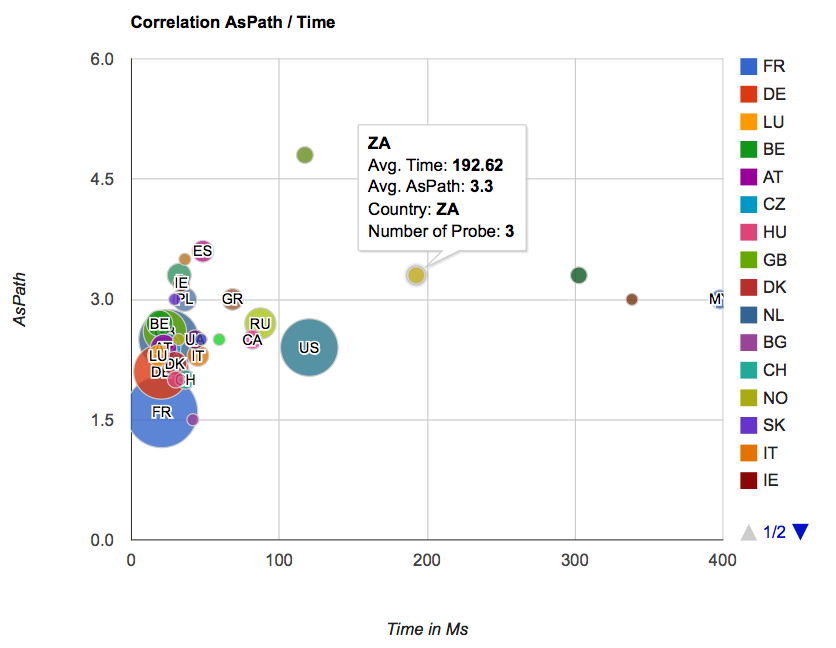
\includegraphics[width=1\linewidth]{illustrations/1-AS-Path-Time-correlation}
	\caption{La corrélation entre la moyenne des AS paths et la moyenne des RTTs \cite{Salim-Gasmi}}
	\label{fig:1-AS-Path-Time-correlationv}
\end{figure}


Ensuite, S. Gasmi a mesuré le RTT entre des sondes Atlas dans le monde et son ancre, il a aussi visualisé le nombre de sauts parcourus entre des sondes Atlas à travers le monde et son ancre. Ces deux visualisations permettent d'avoir une idée sur la latence entre certains pays et le pays de l'ancre en question. Plus de détails sur l'approche sont disponibles dans \cite{Salim-Gasmi}.


\paragraph{La vérification de la cohérence du Traceroute}~

Les chemins parcourus par traceroute pour aller d'une source $s$ vers une destination $d$ changent au cours du temps pour plusieurs raisons. Par exemple, suite   à un changement BGP, à une  répartition des charges, à des pannes des routeurs,  à des pannes des liens physiques, etc.

\textit{Traceroute Consistency Check} peut reprendre les chemins obtenus via traceroute au cours du temps . L'objectif est de suivre les  n\oe{}uds apparaissant dans le chemin allant de  $s$ à $d$ aux instants $t$, $t+1$, $t+2$, etc, et cela afin de voir les n\oe{}uds traversés plus fréquemment au cours du temps. Le chemin est mis à jour via Atlas streaming API. 

L'outil proposé dessine les chemins traceroute comme étant un graphe dirigé, chaque n\oe{}ud est coloré suivant sa cohérence. Le code source du projet est disponible sur GitHub \cite{Traceroute-consistency-check}. La Figure \ref{fig:Traceroute-consistency-check} présente un exemple de la visualisation proposée. Ce résultat concerne la mesure $1663314$ \footnote{Source : \url{https://atlas.ripe.net/measurements/1663314/}, consultée le $05/08/2018$.}. Ce sont des traceroutes à destination de l'adresse $213.171.160.1$, effectués entre le $02/05/2014$ $13:00$ et le $03/05/2014$ $15:00$.

\begin{figure}[H]
	\centering
	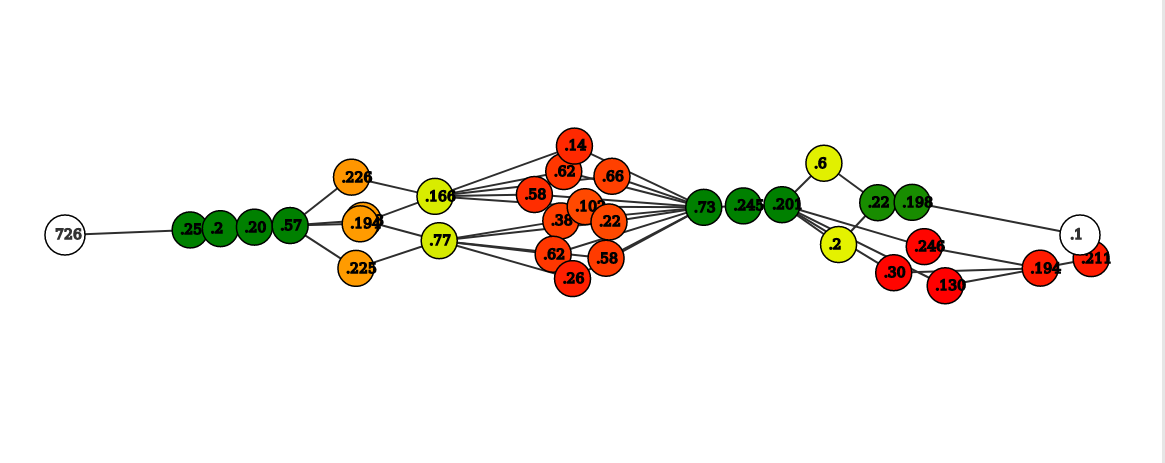
\includegraphics[width=1\linewidth]{illustrations/traceroute-consitance.png}
	\caption{Visualisation des changements des chemins traceroute \cite{Traceroute-consistency-check}}
	\label{fig:Traceroute-consistency-check}
\end{figure}

\paragraph{BGP+traceroute} ~

C'est une combinaison des données BGP (RIPE RIS) et traceroute (RIPE Atlas). L'objectif de ce projet est de partir d'un AS path pour enfin géolocaliser les ASs. 
L'idée est de prendre un AS path des données RIPE RIS, puis, récupérer le préfixe (bloc d'adresses IP) annoncé via cet AS path, ensuite, lancer un traceroute vers une des adresses du bloc. Enfin, géolocaliser les ASs via les données du traceroute. 
Le code source et la présentation de ce projet sont disponibles GitHub \cite{bgp-traceroutes,pres-bgp-traceroute}. 


\paragraph{BGP Atlas Monitor (BAM)} ~

Le projet \textit{BAM} vise la visualisation , en temps réel,  des informations utiles pour les opérateurs des réseaux. Par exemple, BAM montre  la visibilité des préfixes obtenus par RIPE RIS. De plus,  il est possible de voir  le délai du \textit{ping} obtenu via les sondes   Atlas. Le code source est disponible sur  GitHub \cite{bam}. En fournissant un ASN (identifiant d'un AS), \textit{BAM} récupère les préfixes IPv4 et IPv6 et leur visibilité et il montre aussi les sondes dans cet AS. L'outil offre  les  fonctionnalités suivantes :
\begin{itemize}
	\item[--] les préfixes annoncés par un ASN;
	\item[--] la visibilité d'un ASN;
	\item[--] la visibilité d'un préfixe;
	\item[--] la liste des sondes par AS;
	\item[--] les objets  route des préfixes.
\end{itemize}

\paragraph{Prédiction des routeurs provoquant la perte des paquets }~

Dans l'étude \cite{DBLP:journals/corr/FontugneAPB16}, R. Fontugne et al. ont modélisé le comportement  des routeurs, ils ont développé un modèle qui permet d'estimer l'endroit de la  perte des paquets. A partir des traceroutes passant par un routeur \textit{r} à une destination \textit{d}, ils ont construit un modèle de forwarding pour ce routeur. Ce modèle reprend les prochains sauts (routeurs) et la fréquence de passage par ces derniers. Si le routeur \textit{r} change le prochain saut qui a eu "l'habitude" de traverser  pour atteindre \textit{d}, alors cela pour être un indicateur de l'origine  de la perte des paquets.

\subsection{Le suivi des détours dans un trafic local}

Dans leur travail \cite{Emile-Aben-IXP-countries}, E. Aben et al. avaient l'objectif de  voir comment les mesures du RIPE Atlas peuvent fournir un aperçu sur le chemin du trafic local à un pays. Précisément si ce trafic traverse un autre pays en revenant au pays du départ.  Ce qui pourrait  aider à améliorer les performances et l'efficacité des IXPs.  L'objectif est  d'analyser les chemins identifiés dans le trafic d'Internet entre les sondes  Atlas dans un pays donné et essayer d'identifier si le trafic  traverse les IXPs.


France-IX est un point d'échange Internet (IXP) français créé en juin 2010. Afin d'apprendre la topologie de routage, un RIS route collector (RRC21) a été installé au sein du France-IX. Actuellement, la France compte $755$ sondes  Atlas et $9$ ancres. Une ancre sur les $9$ est installée au sein de France-IX.

Une des questions posées c'est de savoir si le trafic local de la France reste localement.  Les sondes  Atlas ne permettent pas de mesurer le trafic entre deux points, alors qu' elles permettent de calculer le chemin entre deux points, adresses IP, ce qui permet d'inférer les sauts par lesquels il passe le trafic. Le travail \cite{France-IX} s'intéresse au trafic depuis et vers une sonde en France en se basant sur l'étude \cite{Emile-Aben-IXP-countries}.


Les résultats obtenus de l'analyse des détours peuvent être intéressants pour les opérateurs des réseaux afin d'améliorer leurs services, ainsi intéressants pour les IXPs tels qu'ils peuvent  proposer des services de peering dans les endroits où il le faut.


\subsection{Visualisation : indicateurs et dashboard}

L'objectif de certains travaux est  d'exploiter les données collectées par les sondes Atlas pour concevoir des tableaux des indicateurs. Par exemple, à partir des données de connexion/déconnexion des sondes Atlas, on peut visualiser les sondes connectées, déconnectées, abandonnées. Un autre projet avait comme objectif la reconstruction d'un graphe reprenant les routeurs (n\oe{}uds) impliqués dans certains traceroutes, ainsi, identifier les n\oe{}uds les plus traversés. D'autres travaux ont repris les détails de la latence, essentiellement, sont les valeurs des RTTs dans les pings et les traceroutes qui permettent de visualiser ce type d'information. 


La liste des travaux basés sur le projet RIPE Atlas est très longue. Nous avons essayé d'énumérer quelques projets, les classer par thèmes, toutefois, ce n'est pas un classement unique, tel qu'on peut retrouver un travail dans plus d'une catégorie, ou bien les classer par un autre classement.

\section{Conclusion}

Dans ce chapitre, nous avons présenté les sondes Atlas et leur fonctionnement, ainsi que quelques travaux ayant impliqué des données collectées par ces sondes.  Ces travaux ont visé différents thèmes, tels que la prise de décision, le suivi des censures, la conception des tableaux de visualisation, etc. Dans le reste de ce document, le choix a été porté sur un sujet lié aux performances des réseaux informatiques. Il s'agit d'un outil de détection des anomalies dans les délais des liens dans les réseaux informatiques, en se basant sur les mesures de traceroute. Une présentation détaillée de l'algorithme de détection est donnée dans le chapitre \ref{chap:algorith-detection}.

%Cet outil donne de meilleure résultat si les données utilisées sont assez grande.  Toutefois, lCependant, ces données sont massives, elles sont  dans l'ordre d'une dizaine de GB rien que pour pour une heure de mesures du type traceroute par exemple, y incluent toutes les destinations.
%C'est pourquoi il faut considérer des outils adaptés. 

%En effet, le chapitre 2 aborde le sujet du Big Data dans ses différentes dimensions. 

%Dans  ce chapitre, nous avons découvert le fonctionnement des sondes Atlas  ainsi que les travaux ayant impliqué les données collectées par ces sondes.  Nous avons appris aussi la nature des données que les sondes Atlas collectent, c'est  crucial pour mener à toute analyse. Vu l'ordre de grandeur de la  quantité de données collectées, les outils traditionnels ne peuvent pas traiter ces données de façon efficace.


%en particulier, à   l'analyse prévue dans le chapitre \ref{chap:implementation}. 


%
\chapter{La détection des anomalies dans les délais d'un lien}

\section{Introduction}

Dans le présent chapitre, nous allons présenter l'outil de détection des anomalies dans les délais d'un lien  conçu dans le cadre du travail de R. Fontugne et al \cite{DBLP:journals/corr/FontugneAPB16}. Nous avons choisi ce travail qui exploite des données massives en vue d'évaluer quelques technologies du Big Data.

\section{Présentation du travail de référence}

\paragraph{Une vue globale du travail de référence}~ 

Le travail de R. Fontugne \cite{DBLP:journals/corr/FontugneAPB16} et al exploite une des mesures effectuées par les sondes Atlas, c'est la requête traceroute. L'idée de ce travail est de collecter les résultats des requêtes traceroutes effectuées par les sondes Atlas, ensuite comparer la référence avec la valeur courante. Cette  référence pour le délai  d'un lien donné   sera mise à jour au fur et à mesure de l'analyse.

\section{Présentation de l'outil de la détection des anomalies }

Les entrées de l'algorithme de la détection est un ensemble de traceroutes. Un traceroute (Traceroute) est un ensemble de sauts (Hop) en plus les informations générales concernant la sonde ayant effectué la requête traceroute et la destination de la requête. Chaque saut est décrit par un ensemble de signaux (Signal), où un signal, dans le présent contexte, décrit le routeur ayant émet une réponse à la sonde Atlas parmi les routeurs traversés avant d'atteindre la destination finale.  Pour le saut $i$, on note trois signaux dont le routeur émettant le signal est $fromij$ avec un RTT égal à $rttij$, avec $j \in [1,3]$ comme illustré dans la figure \ref{fig:traceroute}.

\begin{figure}[H]
	\centering
	\resizebox{\textwidth}{!}{
	% Graphic for TeX using PGF
% Title: /home/hayat/RipeAtlasTraceroutesAnalysis/report/illustrations/traceroute.dia
% Creator: Dia v0.97+git
% CreationDate: Thu Nov 29 12:20:12 2018
% For: hayat
% \usepackage{tikz}
% The following commands are not supported in PSTricks at present
% We define them conditionally, so when they are implemented,
% this pgf file will use them.
\ifx\du\undefined
  \newlength{\du}
\fi
\setlength{\du}{15\unitlength}
\begin{tikzpicture}[even odd rule]
\pgftransformxscale{1.000000}
\pgftransformyscale{-1.000000}
\definecolor{dialinecolor}{rgb}{0.000000, 0.000000, 0.000000}
\pgfsetstrokecolor{dialinecolor}
\pgfsetstrokeopacity{1.000000}
\definecolor{diafillcolor}{rgb}{1.000000, 1.000000, 1.000000}
\pgfsetfillcolor{diafillcolor}
\pgfsetfillopacity{1.000000}
\pgfsetlinewidth{0.100000\du}
\pgfsetdash{}{0pt}
\pgfsetmiterjoin
{\pgfsetcornersarced{\pgfpoint{0.000000\du}{0.000000\du}}\definecolor{diafillcolor}{rgb}{1.000000, 1.000000, 1.000000}
\pgfsetfillcolor{diafillcolor}
\pgfsetfillopacity{1.000000}
\fill (2.487500\du,12.100000\du)--(2.487500\du,14.000000\du)--(5.712500\du,14.000000\du)--(5.712500\du,12.100000\du)--cycle;
}{\pgfsetcornersarced{\pgfpoint{0.000000\du}{0.000000\du}}\definecolor{dialinecolor}{rgb}{0.000000, 0.000000, 0.000000}
\pgfsetstrokecolor{dialinecolor}
\pgfsetstrokeopacity{1.000000}
\draw (2.487500\du,12.100000\du)--(2.487500\du,14.000000\du)--(5.712500\du,14.000000\du)--(5.712500\du,12.100000\du)--cycle;
}% setfont left to latex
\definecolor{dialinecolor}{rgb}{0.000000, 0.000000, 0.000000}
\pgfsetstrokecolor{dialinecolor}
\pgfsetstrokeopacity{1.000000}
\definecolor{diafillcolor}{rgb}{0.000000, 0.000000, 0.000000}
\pgfsetfillcolor{diafillcolor}
\pgfsetfillopacity{1.000000}
\node[anchor=base,inner sep=0pt, outer sep=0pt,color=dialinecolor] at (4.100000\du,13.245000\du){source};
\pgfsetlinewidth{0.100000\du}
\pgfsetdash{}{0pt}
\pgfsetmiterjoin
{\pgfsetcornersarced{\pgfpoint{0.000000\du}{0.000000\du}}\definecolor{diafillcolor}{rgb}{1.000000, 1.000000, 1.000000}
\pgfsetfillcolor{diafillcolor}
\pgfsetfillopacity{1.000000}
\fill (46.257500\du,11.850000\du)--(46.257500\du,13.750000\du)--(50.942500\du,13.750000\du)--(50.942500\du,11.850000\du)--cycle;
}{\pgfsetcornersarced{\pgfpoint{0.000000\du}{0.000000\du}}\definecolor{dialinecolor}{rgb}{0.000000, 0.000000, 0.000000}
\pgfsetstrokecolor{dialinecolor}
\pgfsetstrokeopacity{1.000000}
\draw (46.257500\du,11.850000\du)--(46.257500\du,13.750000\du)--(50.942500\du,13.750000\du)--(50.942500\du,11.850000\du)--cycle;
}% setfont left to latex
\definecolor{dialinecolor}{rgb}{0.000000, 0.000000, 0.000000}
\pgfsetstrokecolor{dialinecolor}
\pgfsetstrokeopacity{1.000000}
\definecolor{diafillcolor}{rgb}{0.000000, 0.000000, 0.000000}
\pgfsetfillcolor{diafillcolor}
\pgfsetfillopacity{1.000000}
\node[anchor=base,inner sep=0pt, outer sep=0pt,color=dialinecolor] at (48.600000\du,12.995000\du){destination};
\pgfsetlinewidth{0.100000\du}
\pgfsetdash{}{0pt}
\pgfsetmiterjoin
\definecolor{diafillcolor}{rgb}{1.000000, 1.000000, 1.000000}
\pgfsetfillcolor{diafillcolor}
\pgfsetfillopacity{1.000000}
\pgfpathellipse{\pgfpoint{11.648369\du}{12.925048\du}}{\pgfpoint{1.195569\du}{0\du}}{\pgfpoint{0\du}{1.078448\du}}
\pgfusepath{fill}
\definecolor{dialinecolor}{rgb}{0.000000, 0.000000, 0.000000}
\pgfsetstrokecolor{dialinecolor}
\pgfsetstrokeopacity{1.000000}
\pgfpathellipse{\pgfpoint{11.648369\du}{12.925048\du}}{\pgfpoint{1.195569\du}{0\du}}{\pgfpoint{0\du}{1.078448\du}}
\pgfusepath{stroke}
% setfont left to latex
\definecolor{dialinecolor}{rgb}{0.000000, 0.000000, 0.000000}
\pgfsetstrokecolor{dialinecolor}
\pgfsetstrokeopacity{1.000000}
\definecolor{diafillcolor}{rgb}{0.000000, 0.000000, 0.000000}
\pgfsetfillcolor{diafillcolor}
\pgfsetfillopacity{1.000000}
\node[anchor=base,inner sep=0pt, outer sep=0pt,color=dialinecolor] at (11.648369\du,13.120048\du){R1};
\pgfsetlinewidth{0.100000\du}
\pgfsetdash{}{0pt}
\pgfsetmiterjoin
\definecolor{diafillcolor}{rgb}{1.000000, 1.000000, 1.000000}
\pgfsetfillcolor{diafillcolor}
\pgfsetfillopacity{1.000000}
\pgfpathellipse{\pgfpoint{21.040569\du}{12.968448\du}}{\pgfpoint{1.195569\du}{0\du}}{\pgfpoint{0\du}{1.078448\du}}
\pgfusepath{fill}
\definecolor{dialinecolor}{rgb}{0.000000, 0.000000, 0.000000}
\pgfsetstrokecolor{dialinecolor}
\pgfsetstrokeopacity{1.000000}
\pgfpathellipse{\pgfpoint{21.040569\du}{12.968448\du}}{\pgfpoint{1.195569\du}{0\du}}{\pgfpoint{0\du}{1.078448\du}}
\pgfusepath{stroke}
% setfont left to latex
\definecolor{dialinecolor}{rgb}{0.000000, 0.000000, 0.000000}
\pgfsetstrokecolor{dialinecolor}
\pgfsetstrokeopacity{1.000000}
\definecolor{diafillcolor}{rgb}{0.000000, 0.000000, 0.000000}
\pgfsetfillcolor{diafillcolor}
\pgfsetfillopacity{1.000000}
\node[anchor=base,inner sep=0pt, outer sep=0pt,color=dialinecolor] at (21.040569\du,13.163448\du){R2};
\pgfsetlinewidth{0.100000\du}
\pgfsetdash{}{0pt}
\pgfsetmiterjoin
\definecolor{diafillcolor}{rgb}{1.000000, 1.000000, 1.000000}
\pgfsetfillcolor{diafillcolor}
\pgfsetfillopacity{1.000000}
\pgfpathellipse{\pgfpoint{29.935569\du}{12.858448\du}}{\pgfpoint{1.195569\du}{0\du}}{\pgfpoint{0\du}{1.078448\du}}
\pgfusepath{fill}
\definecolor{dialinecolor}{rgb}{0.000000, 0.000000, 0.000000}
\pgfsetstrokecolor{dialinecolor}
\pgfsetstrokeopacity{1.000000}
\pgfpathellipse{\pgfpoint{29.935569\du}{12.858448\du}}{\pgfpoint{1.195569\du}{0\du}}{\pgfpoint{0\du}{1.078448\du}}
\pgfusepath{stroke}
% setfont left to latex
\definecolor{dialinecolor}{rgb}{0.000000, 0.000000, 0.000000}
\pgfsetstrokecolor{dialinecolor}
\pgfsetstrokeopacity{1.000000}
\definecolor{diafillcolor}{rgb}{0.000000, 0.000000, 0.000000}
\pgfsetfillcolor{diafillcolor}
\pgfsetfillopacity{1.000000}
\node[anchor=base,inner sep=0pt, outer sep=0pt,color=dialinecolor] at (29.935569\du,13.053448\du){R3};
\pgfsetlinewidth{0.100000\du}
\pgfsetdash{}{0pt}
\pgfsetbuttcap
{
\definecolor{diafillcolor}{rgb}{0.000000, 0.000000, 0.000000}
\pgfsetfillcolor{diafillcolor}
\pgfsetfillopacity{1.000000}
% was here!!!
\definecolor{dialinecolor}{rgb}{0.000000, 0.000000, 0.000000}
\pgfsetstrokecolor{dialinecolor}
\pgfsetstrokeopacity{1.000000}
\draw (5.750239\du,13.017555\du)--(10.452800\du,12.925100\du);
}
\pgfsetlinewidth{0.100000\du}
\pgfsetdash{}{0pt}
\pgfsetbuttcap
{
\definecolor{diafillcolor}{rgb}{0.000000, 0.000000, 0.000000}
\pgfsetfillcolor{diafillcolor}
\pgfsetfillopacity{1.000000}
% was here!!!
\definecolor{dialinecolor}{rgb}{0.000000, 0.000000, 0.000000}
\pgfsetstrokecolor{dialinecolor}
\pgfsetstrokeopacity{1.000000}
\draw (12.844000\du,12.925100\du)--(19.845000\du,12.968448\du);
}
\pgfsetlinewidth{0.100000\du}
\pgfsetdash{}{0pt}
\pgfsetbuttcap
{
\definecolor{diafillcolor}{rgb}{0.000000, 0.000000, 0.000000}
\pgfsetfillcolor{diafillcolor}
\pgfsetfillopacity{1.000000}
% was here!!!
\definecolor{dialinecolor}{rgb}{0.000000, 0.000000, 0.000000}
\pgfsetstrokecolor{dialinecolor}
\pgfsetstrokeopacity{1.000000}
\draw (22.236138\du,12.968448\du)--(28.690239\du,12.876240\du);
}
\pgfsetlinewidth{0.100000\du}
\pgfsetdash{}{0pt}
\pgfsetbuttcap
{
\definecolor{diafillcolor}{rgb}{0.000000, 0.000000, 0.000000}
\pgfsetfillcolor{diafillcolor}
\pgfsetfillopacity{1.000000}
% was here!!!
\definecolor{dialinecolor}{rgb}{0.000000, 0.000000, 0.000000}
\pgfsetstrokecolor{dialinecolor}
\pgfsetstrokeopacity{1.000000}
\draw (40.536100\du,12.868400\du)--(46.257500\du,12.800000\du);
}
% setfont left to latex
\definecolor{dialinecolor}{rgb}{0.000000, 0.000000, 0.000000}
\pgfsetstrokecolor{dialinecolor}
\pgfsetstrokeopacity{1.000000}
\definecolor{diafillcolor}{rgb}{0.000000, 0.000000, 0.000000}
\pgfsetfillcolor{diafillcolor}
\pgfsetfillopacity{1.000000}
\node[anchor=base west,inner sep=0pt,outer sep=0pt,color=dialinecolor] at (9.050000\du,11.000000\du){rtt11, rtt12, rtt13};
% setfont left to latex
\definecolor{dialinecolor}{rgb}{0.000000, 0.000000, 0.000000}
\pgfsetstrokecolor{dialinecolor}
\pgfsetstrokeopacity{1.000000}
\definecolor{diafillcolor}{rgb}{0.000000, 0.000000, 0.000000}
\pgfsetfillcolor{diafillcolor}
\pgfsetfillopacity{1.000000}
\node[anchor=base west,inner sep=0pt,outer sep=0pt,color=dialinecolor] at (17.995000\du,11.085000\du){rtt21, rtt22, rtt23};
% setfont left to latex
\definecolor{dialinecolor}{rgb}{0.000000, 0.000000, 0.000000}
\pgfsetstrokecolor{dialinecolor}
\pgfsetstrokeopacity{1.000000}
\definecolor{diafillcolor}{rgb}{0.000000, 0.000000, 0.000000}
\pgfsetfillcolor{diafillcolor}
\pgfsetfillopacity{1.000000}
\node[anchor=base west,inner sep=0pt,outer sep=0pt,color=dialinecolor] at (26.845000\du,11.035000\du){rtt31, rtt32, rtt33};
\pgfsetlinewidth{0.100000\du}
\pgfsetdash{}{0pt}
\pgfsetmiterjoin
\definecolor{diafillcolor}{rgb}{1.000000, 1.000000, 1.000000}
\pgfsetfillcolor{diafillcolor}
\pgfsetfillopacity{1.000000}
\pgfpathellipse{\pgfpoint{39.340569\du}{12.868448\du}}{\pgfpoint{1.195569\du}{0\du}}{\pgfpoint{0\du}{1.078448\du}}
\pgfusepath{fill}
\definecolor{dialinecolor}{rgb}{0.000000, 0.000000, 0.000000}
\pgfsetstrokecolor{dialinecolor}
\pgfsetstrokeopacity{1.000000}
\pgfpathellipse{\pgfpoint{39.340569\du}{12.868448\du}}{\pgfpoint{1.195569\du}{0\du}}{\pgfpoint{0\du}{1.078448\du}}
\pgfusepath{stroke}
% setfont left to latex
\definecolor{dialinecolor}{rgb}{0.000000, 0.000000, 0.000000}
\pgfsetstrokecolor{dialinecolor}
\pgfsetstrokeopacity{1.000000}
\definecolor{diafillcolor}{rgb}{0.000000, 0.000000, 0.000000}
\pgfsetfillcolor{diafillcolor}
\pgfsetfillopacity{1.000000}
\node[anchor=base,inner sep=0pt, outer sep=0pt,color=dialinecolor] at (39.340569\du,13.063448\du){Ri};
\pgfsetlinewidth{0.100000\du}
\pgfsetdash{{\pgflinewidth}{0.220000\du}}{0cm}
\pgfsetbuttcap
{
\definecolor{diafillcolor}{rgb}{0.000000, 0.000000, 0.000000}
\pgfsetfillcolor{diafillcolor}
\pgfsetfillopacity{1.000000}
% was here!!!
\definecolor{dialinecolor}{rgb}{0.000000, 0.000000, 0.000000}
\pgfsetstrokecolor{dialinecolor}
\pgfsetstrokeopacity{1.000000}
\draw (31.131138\du,12.858448\du)--(37.000000\du,12.800000\du);
}
% setfont left to latex
\definecolor{dialinecolor}{rgb}{0.000000, 0.000000, 0.000000}
\pgfsetstrokecolor{dialinecolor}
\pgfsetstrokeopacity{1.000000}
\definecolor{diafillcolor}{rgb}{0.000000, 0.000000, 0.000000}
\pgfsetfillcolor{diafillcolor}
\pgfsetfillopacity{1.000000}
\node[anchor=base west,inner sep=0pt,outer sep=0pt,color=dialinecolor] at (36.645000\du,10.985000\du){$ rtt_{i,1} $, $ rtt_{i,2} $, $ rtt_{i,3} $};
% setfont left to latex
\definecolor{dialinecolor}{rgb}{0.000000, 0.000000, 0.000000}
\pgfsetstrokecolor{dialinecolor}
\pgfsetstrokeopacity{1.000000}
\definecolor{diafillcolor}{rgb}{0.000000, 0.000000, 0.000000}
\pgfsetfillcolor{diafillcolor}
\pgfsetfillopacity{1.000000}
\node[anchor=base west,inner sep=0pt,outer sep=0pt,color=dialinecolor] at (8.245000\du,10.035000\du){$from_{1,1}$, $from_{1,2}$, $from_{1,3}$};
% setfont left to latex
\definecolor{dialinecolor}{rgb}{0.000000, 0.000000, 0.000000}
\pgfsetstrokecolor{dialinecolor}
\pgfsetstrokeopacity{1.000000}
\definecolor{diafillcolor}{rgb}{0.000000, 0.000000, 0.000000}
\pgfsetfillcolor{diafillcolor}
\pgfsetfillopacity{1.000000}
\node[anchor=base west,inner sep=0pt,outer sep=0pt,color=dialinecolor] at (16.945000\du,10.035000\du){$ from_{2,1} $, $ from_{2,2} $, $ from_{2,3} $};
% setfont left to latex
\definecolor{dialinecolor}{rgb}{0.000000, 0.000000, 0.000000}
\pgfsetstrokecolor{dialinecolor}
\pgfsetstrokeopacity{1.000000}
\definecolor{diafillcolor}{rgb}{0.000000, 0.000000, 0.000000}
\pgfsetfillcolor{diafillcolor}
\pgfsetfillopacity{1.000000}
\node[anchor=base west,inner sep=0pt,outer sep=0pt,color=dialinecolor] at (25.945000\du,10.035000\du){from31, from32, from33};
% setfont left to latex
\definecolor{dialinecolor}{rgb}{0.000000, 0.000000, 0.000000}
\pgfsetstrokecolor{dialinecolor}
\pgfsetstrokeopacity{1.000000}
\definecolor{diafillcolor}{rgb}{0.000000, 0.000000, 0.000000}
\pgfsetfillcolor{diafillcolor}
\pgfsetfillopacity{1.000000}
\node[anchor=base west,inner sep=0pt,outer sep=0pt,color=dialinecolor] at (35.390000\du,9.975000\du){fromi1, fromi2, fromi3};
% setfont left to latex
\definecolor{dialinecolor}{rgb}{0.000000, 0.000000, 0.000000}
\pgfsetstrokecolor{dialinecolor}
\pgfsetstrokeopacity{1.000000}
\definecolor{diafillcolor}{rgb}{0.000000, 0.000000, 0.000000}
\pgfsetfillcolor{diafillcolor}
\pgfsetfillopacity{1.000000}
\node[anchor=base west,inner sep=0pt,outer sep=0pt,color=dialinecolor] at (10.900000\du,9.000000\du){saut 1};
% setfont left to latex
\definecolor{dialinecolor}{rgb}{0.000000, 0.000000, 0.000000}
\pgfsetstrokecolor{dialinecolor}
\pgfsetstrokeopacity{1.000000}
\definecolor{diafillcolor}{rgb}{0.000000, 0.000000, 0.000000}
\pgfsetfillcolor{diafillcolor}
\pgfsetfillopacity{1.000000}
\node[anchor=base west,inner sep=0pt,outer sep=0pt,color=dialinecolor] at (19.795000\du,8.985000\du){saut 2};
% setfont left to latex
\definecolor{dialinecolor}{rgb}{0.000000, 0.000000, 0.000000}
\pgfsetstrokecolor{dialinecolor}
\pgfsetstrokeopacity{1.000000}
\definecolor{diafillcolor}{rgb}{0.000000, 0.000000, 0.000000}
\pgfsetfillcolor{diafillcolor}
\pgfsetfillopacity{1.000000}
\node[anchor=base west,inner sep=0pt,outer sep=0pt,color=dialinecolor] at (28.690000\du,9.025000\du){saut 3};
% setfont left to latex
\definecolor{dialinecolor}{rgb}{0.000000, 0.000000, 0.000000}
\pgfsetstrokecolor{dialinecolor}
\pgfsetstrokeopacity{1.000000}
\definecolor{diafillcolor}{rgb}{0.000000, 0.000000, 0.000000}
\pgfsetfillcolor{diafillcolor}
\pgfsetfillopacity{1.000000}
\node[anchor=base west,inner sep=0pt,outer sep=0pt,color=dialinecolor] at (37.785000\du,9.015000\du){saut i};
\end{tikzpicture}

}
	\caption{}
	\label{fig:traceroute}
\end{figure}

\subsection{Paramètres de l'algorithme de la détection}

\begin{itemize}
		\item  Objectif : suivre l'évolution du délais d'un lien au cours du temps en suivant son RTT différentiel par période du temps (\textit{timeWindow}).
	\item Entrées : l'ensemble des traceroutes stockés dans un fichier, date de début de l'analyse \textit{start}, date de la fin de l'analyse \textit{end}, lien à analyser (\textit{link}) et la fenêtre de l'analyse (\textit{timeWindow}).
	\item Sorties : les dates pendant lesquelles des anomalies ont été détectées.
\end{itemize}

Soient $ d_1 $,$  d_2 $, ..., $ d_N $ les périodes entre \textit{start} et \textit{end} où

\begin{center}
	 $  d_{i+1} $ - $  d_{i} $ = $  d_{j+1} $ - $  d_{j} $ = \textit{step} \footnote{\textit{step} est la durée d'une période en secondes, $3600$ pour fenêtre d'une heure.}
\end{center}
 
 pour tout $ i $ et $ j $ dans$  [1,N] $
\subsection{Le processus de la détection des anomalies dans les délais d'un lien}\label{steps-rtt-analysis}

On distingue trois grandes étapes dans le processus de la détection des anomalies, dont les détails sont donnés dans la figure \ref{fig:process-rttanalysis_tex}. La première étape a pour objectif de trier les traceroutes à analyser par période (étape 1). La deuxième étape désigne les opérations à appliquer sur les traceroutes d'une période (étapes entre 2 et 6). A la fin de la préparation des traceroutes de toutes les périodes, la troisième étape est dédiée à la comparaison des délais avec les valeurs de la référence (étape 7).
\paragraph{1. Trier les traceroutes } à analyser par \textit{timeWindow}. En effet, chaque $d_i$ est associé à un ensemble de traceroutes ayant été effectués entre $d_i$ et $d_i + step$ \footnote{Chaque traceroute reprend le temps pendant lequel il était effectué.}. 

\begin{figure}[H]
	\centering
	\captionsetup{justification=centering}
	% Graphic for TeX using PGF
% Title: /home/hayat/RipeAtlasTraceroutesAnalysis/report/illustrations/timing.dia
% Creator: Dia v0.97+git
% CreationDate: Mon Dec  3 23:19:01 2018
% For: hayat
% \usepackage{tikz}
% The following commands are not supported in PSTricks at present
% We define them conditionally, so when they are implemented,
% this pgf file will use them.
\ifx\du\undefined
  \newlength{\du}
\fi
\setlength{\du}{15\unitlength}
\begin{tikzpicture}[even odd rule]
\pgftransformxscale{1.000000}
\pgftransformyscale{-1.000000}
\definecolor{dialinecolor}{rgb}{0.000000, 0.000000, 0.000000}
\pgfsetstrokecolor{dialinecolor}
\pgfsetstrokeopacity{1.000000}
\definecolor{diafillcolor}{rgb}{1.000000, 1.000000, 1.000000}
\pgfsetfillcolor{diafillcolor}
\pgfsetfillopacity{1.000000}
\pgfsetlinewidth{0.100000\du}
\pgfsetdash{}{0pt}
\pgfsetbuttcap
{
\definecolor{diafillcolor}{rgb}{0.000000, 0.000000, 0.000000}
\pgfsetfillcolor{diafillcolor}
\pgfsetfillopacity{1.000000}
% was here!!!
}
\definecolor{dialinecolor}{rgb}{0.000000, 0.000000, 0.000000}
\pgfsetstrokecolor{dialinecolor}
\pgfsetstrokeopacity{1.000000}
\draw (34.600000\du,6.050000\du)--(40.550000\du,6.000000\du);
\pgfsetlinewidth{0.100000\du}
\pgfsetdash{}{0pt}
\pgfsetmiterjoin
\pgfsetbuttcap
\definecolor{dialinecolor}{rgb}{0.000000, 0.000000, 0.000000}
\pgfsetstrokecolor{dialinecolor}
\pgfsetstrokeopacity{1.000000}
\draw (35.097882\du,5.795807\du)--(35.102083\du,6.295790\du);
\pgfsetlinewidth{0.100000\du}
\pgfsetdash{}{0pt}
\pgfsetmiterjoin
\pgfsetbuttcap
\definecolor{dialinecolor}{rgb}{0.000000, 0.000000, 0.000000}
\pgfsetstrokecolor{dialinecolor}
\pgfsetstrokeopacity{1.000000}
\draw (40.052118\du,6.254193\du)--(40.047917\du,5.754210\du);
% setfont left to latex
\definecolor{dialinecolor}{rgb}{0.000000, 0.000000, 0.000000}
\pgfsetstrokecolor{dialinecolor}
\pgfsetstrokeopacity{1.000000}
\definecolor{diafillcolor}{rgb}{0.000000, 0.000000, 0.000000}
\pgfsetfillcolor{diafillcolor}
\pgfsetfillopacity{1.000000}
\node[anchor=base west,inner sep=0pt,outer sep=0pt,color=dialinecolor] at (14.800200\du,8.464650\du){start};
% setfont left to latex
\definecolor{dialinecolor}{rgb}{0.000000, 0.000000, 0.000000}
\pgfsetstrokecolor{dialinecolor}
\pgfsetstrokeopacity{1.000000}
\definecolor{diafillcolor}{rgb}{0.000000, 0.000000, 0.000000}
\pgfsetfillcolor{diafillcolor}
\pgfsetfillopacity{1.000000}
\node[anchor=base west,inner sep=0pt,outer sep=0pt,color=dialinecolor] at (39.375600\du,7.990890\du){end};
% setfont left to latex
\definecolor{dialinecolor}{rgb}{0.000000, 0.000000, 0.000000}
\pgfsetstrokecolor{dialinecolor}
\pgfsetstrokeopacity{1.000000}
\definecolor{diafillcolor}{rgb}{0.000000, 0.000000, 0.000000}
\pgfsetfillcolor{diafillcolor}
\pgfsetfillopacity{1.000000}
\node[anchor=base west,inner sep=0pt,outer sep=0pt,color=dialinecolor] at (24.374800\du,8.977310\du){Périodes de l'analyse};
% setfont left to latex
\definecolor{dialinecolor}{rgb}{0.000000, 0.000000, 0.000000}
\pgfsetstrokecolor{dialinecolor}
\pgfsetstrokeopacity{1.000000}
\definecolor{diafillcolor}{rgb}{0.000000, 0.000000, 0.000000}
\pgfsetfillcolor{diafillcolor}
\pgfsetfillopacity{1.000000}
\node[anchor=base west,inner sep=0pt,outer sep=0pt,color=dialinecolor] at (14.950000\du,7.200000\du){d1};
\pgfsetlinewidth{0.100000\du}
\pgfsetdash{}{0pt}
\pgfsetbuttcap
{
\definecolor{diafillcolor}{rgb}{0.000000, 0.000000, 0.000000}
\pgfsetfillcolor{diafillcolor}
\pgfsetfillopacity{1.000000}
% was here!!!
}
\definecolor{dialinecolor}{rgb}{0.000000, 0.000000, 0.000000}
\pgfsetstrokecolor{dialinecolor}
\pgfsetstrokeopacity{1.000000}
\draw (29.656800\du,6.066270\du)--(35.606800\du,6.016270\du);
\pgfsetlinewidth{0.100000\du}
\pgfsetdash{}{0pt}
\pgfsetmiterjoin
\pgfsetbuttcap
\definecolor{dialinecolor}{rgb}{0.000000, 0.000000, 0.000000}
\pgfsetstrokecolor{dialinecolor}
\pgfsetstrokeopacity{1.000000}
\draw (30.154682\du,5.812077\du)--(30.158883\du,6.312060\du);
\pgfsetlinewidth{0.100000\du}
\pgfsetdash{}{0pt}
\pgfsetmiterjoin
\pgfsetbuttcap
\definecolor{dialinecolor}{rgb}{0.000000, 0.000000, 0.000000}
\pgfsetstrokecolor{dialinecolor}
\pgfsetstrokeopacity{1.000000}
\draw (35.108918\du,6.270463\du)--(35.104717\du,5.770480\du);
\pgfsetlinewidth{0.100000\du}
\pgfsetdash{}{0pt}
\pgfsetbuttcap
{
\definecolor{diafillcolor}{rgb}{0.000000, 0.000000, 0.000000}
\pgfsetfillcolor{diafillcolor}
\pgfsetfillopacity{1.000000}
% was here!!!
}
\definecolor{dialinecolor}{rgb}{0.000000, 0.000000, 0.000000}
\pgfsetstrokecolor{dialinecolor}
\pgfsetstrokeopacity{1.000000}
\draw (24.701800\du,6.106100\du)--(30.651800\du,6.056100\du);
\pgfsetlinewidth{0.100000\du}
\pgfsetdash{}{0pt}
\pgfsetmiterjoin
\pgfsetbuttcap
\definecolor{dialinecolor}{rgb}{0.000000, 0.000000, 0.000000}
\pgfsetstrokecolor{dialinecolor}
\pgfsetstrokeopacity{1.000000}
\draw (25.199682\du,5.851907\du)--(25.203883\du,6.351890\du);
\pgfsetlinewidth{0.100000\du}
\pgfsetdash{}{0pt}
\pgfsetmiterjoin
\pgfsetbuttcap
\definecolor{dialinecolor}{rgb}{0.000000, 0.000000, 0.000000}
\pgfsetstrokecolor{dialinecolor}
\pgfsetstrokeopacity{1.000000}
\draw (30.153918\du,6.310293\du)--(30.149717\du,5.810310\du);
\pgfsetlinewidth{0.100000\du}
\pgfsetdash{}{0pt}
\pgfsetbuttcap
{
\definecolor{diafillcolor}{rgb}{0.000000, 0.000000, 0.000000}
\pgfsetfillcolor{diafillcolor}
\pgfsetfillopacity{1.000000}
% was here!!!
}
\definecolor{dialinecolor}{rgb}{0.000000, 0.000000, 0.000000}
\pgfsetstrokecolor{dialinecolor}
\pgfsetstrokeopacity{1.000000}
\draw (19.796600\du,6.121020\du)--(25.746600\du,6.071020\du);
\pgfsetlinewidth{0.100000\du}
\pgfsetdash{}{0pt}
\pgfsetmiterjoin
\pgfsetbuttcap
\definecolor{dialinecolor}{rgb}{0.000000, 0.000000, 0.000000}
\pgfsetstrokecolor{dialinecolor}
\pgfsetstrokeopacity{1.000000}
\draw (20.294482\du,5.866827\du)--(20.298683\du,6.366810\du);
\pgfsetlinewidth{0.100000\du}
\pgfsetdash{}{0pt}
\pgfsetmiterjoin
\pgfsetbuttcap
\definecolor{dialinecolor}{rgb}{0.000000, 0.000000, 0.000000}
\pgfsetstrokecolor{dialinecolor}
\pgfsetstrokeopacity{1.000000}
\draw (25.248718\du,6.325213\du)--(25.244517\du,5.825230\du);
\pgfsetlinewidth{0.100000\du}
\pgfsetdash{}{0pt}
\pgfsetbuttcap
{
\definecolor{diafillcolor}{rgb}{0.000000, 0.000000, 0.000000}
\pgfsetfillcolor{diafillcolor}
\pgfsetfillopacity{1.000000}
% was here!!!
}
\definecolor{dialinecolor}{rgb}{0.000000, 0.000000, 0.000000}
\pgfsetstrokecolor{dialinecolor}
\pgfsetstrokeopacity{1.000000}
\draw (14.841600\du,6.135940\du)--(20.791600\du,6.085940\du);
\pgfsetlinewidth{0.100000\du}
\pgfsetdash{}{0pt}
\pgfsetmiterjoin
\pgfsetbuttcap
\definecolor{dialinecolor}{rgb}{0.000000, 0.000000, 0.000000}
\pgfsetstrokecolor{dialinecolor}
\pgfsetstrokeopacity{1.000000}
\draw (15.339482\du,5.881747\du)--(15.343683\du,6.381730\du);
\pgfsetlinewidth{0.100000\du}
\pgfsetdash{}{0pt}
\pgfsetmiterjoin
\pgfsetbuttcap
\definecolor{dialinecolor}{rgb}{0.000000, 0.000000, 0.000000}
\pgfsetstrokecolor{dialinecolor}
\pgfsetstrokeopacity{1.000000}
\draw (20.293718\du,6.340133\du)--(20.289517\du,5.840150\du);
% setfont left to latex
\definecolor{dialinecolor}{rgb}{0.000000, 0.000000, 0.000000}
\pgfsetstrokecolor{dialinecolor}
\pgfsetstrokeopacity{1.000000}
\definecolor{diafillcolor}{rgb}{0.000000, 0.000000, 0.000000}
\pgfsetfillcolor{diafillcolor}
\pgfsetfillopacity{1.000000}
\node[anchor=base west,inner sep=0pt,outer sep=0pt,color=dialinecolor] at (19.845000\du,7.235000\du){d2};
% setfont left to latex
\definecolor{dialinecolor}{rgb}{0.000000, 0.000000, 0.000000}
\pgfsetstrokecolor{dialinecolor}
\pgfsetstrokeopacity{1.000000}
\definecolor{diafillcolor}{rgb}{0.000000, 0.000000, 0.000000}
\pgfsetfillcolor{diafillcolor}
\pgfsetfillopacity{1.000000}
\node[anchor=base west,inner sep=0pt,outer sep=0pt,color=dialinecolor] at (24.750000\du,7.300000\du){d3};
% setfont left to latex
\definecolor{dialinecolor}{rgb}{0.000000, 0.000000, 0.000000}
\pgfsetstrokecolor{dialinecolor}
\pgfsetstrokeopacity{1.000000}
\definecolor{diafillcolor}{rgb}{0.000000, 0.000000, 0.000000}
\pgfsetfillcolor{diafillcolor}
\pgfsetfillopacity{1.000000}
\node[anchor=base west,inner sep=0pt,outer sep=0pt,color=dialinecolor] at (29.740000\du,7.175000\du){di};
% setfont left to latex
\definecolor{dialinecolor}{rgb}{0.000000, 0.000000, 0.000000}
\pgfsetstrokecolor{dialinecolor}
\pgfsetstrokeopacity{1.000000}
\definecolor{diafillcolor}{rgb}{0.000000, 0.000000, 0.000000}
\pgfsetfillcolor{diafillcolor}
\pgfsetfillopacity{1.000000}
\node[anchor=base west,inner sep=0pt,outer sep=0pt,color=dialinecolor] at (34.685000\du,7.165000\du){di+1};
\pgfsetlinewidth{0.100000\du}
\pgfsetdash{}{0pt}
\pgfsetbuttcap
\definecolor{dialinecolor}{rgb}{0.000000, 0.000000, 0.000000}
\pgfsetstrokecolor{dialinecolor}
\pgfsetstrokeopacity{1.000000}
\pgfpathmoveto{\pgfpoint{25.180033\du}{4.900033\du}}
\pgfpatharc{315}{226}{3.501250\du and 3.501250\du}
\pgfusepath{stroke}
% setfont left to latex
\definecolor{dialinecolor}{rgb}{0.000000, 0.000000, 0.000000}
\pgfsetstrokecolor{dialinecolor}
\pgfsetstrokeopacity{1.000000}
\definecolor{diafillcolor}{rgb}{0.000000, 0.000000, 0.000000}
\pgfsetfillcolor{diafillcolor}
\pgfsetfillopacity{1.000000}
\node[anchor=base west,inner sep=0pt,outer sep=0pt,color=dialinecolor] at (20.780000\du,3.400000\du){timeWindow};
\pgfsetlinewidth{0.100000\du}
\pgfsetdash{}{0pt}
\pgfsetbuttcap
\definecolor{dialinecolor}{rgb}{0.000000, 0.000000, 0.000000}
\pgfsetstrokecolor{dialinecolor}
\pgfsetstrokeopacity{1.000000}
\pgfpathmoveto{\pgfpoint{29.975033\du}{4.885033\du}}
\pgfpatharc{315}{226}{3.501250\du and 3.501250\du}
\pgfusepath{stroke}
% setfont left to latex
\definecolor{dialinecolor}{rgb}{0.000000, 0.000000, 0.000000}
\pgfsetstrokecolor{dialinecolor}
\pgfsetstrokeopacity{1.000000}
\definecolor{diafillcolor}{rgb}{0.000000, 0.000000, 0.000000}
\pgfsetfillcolor{diafillcolor}
\pgfsetfillopacity{1.000000}
\node[anchor=base west,inner sep=0pt,outer sep=0pt,color=dialinecolor] at (25.675000\du,3.485000\du){timeWindow};
\pgfsetlinewidth{0.100000\du}
\pgfsetdash{}{0pt}
\pgfsetbuttcap
\definecolor{dialinecolor}{rgb}{0.000000, 0.000000, 0.000000}
\pgfsetstrokecolor{dialinecolor}
\pgfsetstrokeopacity{1.000000}
\pgfpathmoveto{\pgfpoint{20.275033\du}{4.785033\du}}
\pgfpatharc{315}{226}{3.501250\du and 3.501250\du}
\pgfusepath{stroke}
% setfont left to latex
\definecolor{dialinecolor}{rgb}{0.000000, 0.000000, 0.000000}
\pgfsetstrokecolor{dialinecolor}
\pgfsetstrokeopacity{1.000000}
\definecolor{diafillcolor}{rgb}{0.000000, 0.000000, 0.000000}
\pgfsetfillcolor{diafillcolor}
\pgfsetfillopacity{1.000000}
\node[anchor=base west,inner sep=0pt,outer sep=0pt,color=dialinecolor] at (16.025000\du,3.435000\du){timeWindow};
\end{tikzpicture}

	\caption{}
	\label{fig:timing_tex}
\end{figure}


Les opérations  (2 à 6) concernent  les traceroutes par tout $d_i$.  

\paragraph{2. Vérification de la validité de chaque traceroute }. Ces vérifications reprennent les points suivants:
\begin{itemize}
	\item élimination des traceroutes échoués complètement;
	\item élimination du signal contenant une adresse IP privée;
	\item élimination du signal qui ne contient pas un RTT ou celui qui contient un RTT négatif;
	\item  élimination du signal échoué.
\end{itemize}

\paragraph{3. Calcul de la médiane des RTTs par saut.} Pour tout saut d'un traceroute,  on calcul la médiane des RTTs par adresse IP. Soit le saut $h =\{s \}$ où $s$ est un  Signal, mediane\_rtt ($h$) =  $\{median(\{s.rtt\})\}$  pour tout signal $s$ ayant la même adresse IP. Autrement dit, le nouveau saut du traceroute est reconstruit en regroupant les signaux par adresse IP et ensuite en calculant leurs RTTs. 




\paragraph{4. Inférence des liens topologiques par traceroute.} Un lien topologique est formé par chaque deux routeurs consécutifs. Ce sont les deux routeurs des deux sauts consécutifs. De manière générale, la figure \ref{fig:link-inference} illustre la constitution des liens possibles  dans un traceroute. Soient  RAi, avec $i \in [1,N]$,  l'ensemble des routeurs pour le saut A et RBj, avec $j \in [1,M]$, l'ensemble  des routeurs pour le saut B, avec N et M deux entiers.



Ainsi, les liens  construits sont ceux partant de tout RAi vers tout RBj, où A et B sont deux sauts consécutifs. A l'issue de cette étape, pour tout traceroute, on obtient la liste des liens possibles tout en reprenant des informations générales de la requête traceroute.
\begin{figure}[H]
	\centering
	\captionsetup{justification=centering}
	%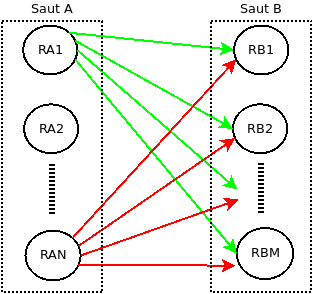
\includegraphics[width=0.5\linewidth]{illustrations/link-inference}
	% Graphic for TeX using PGF
% Title: /home/hayat/RipeAtlasTraceroutesAnalysis/report/illustrations/link-inference.dia
% Creator: Dia v0.97+git
% CreationDate: Thu Nov 29 20:58:09 2018
% For: hayat
% \usepackage{tikz}
% The following commands are not supported in PSTricks at present
% We define them conditionally, so when they are implemented,
% this pgf file will use them.
\ifx\du\undefined
  \newlength{\du}
\fi
\setlength{\du}{15\unitlength}
\begin{tikzpicture}[even odd rule]
\pgftransformxscale{1.000000}
\pgftransformyscale{-1.000000}
\definecolor{dialinecolor}{rgb}{0.000000, 0.000000, 0.000000}
\pgfsetstrokecolor{dialinecolor}
\pgfsetstrokeopacity{1.000000}
\definecolor{diafillcolor}{rgb}{1.000000, 1.000000, 1.000000}
\pgfsetfillcolor{diafillcolor}
\pgfsetfillopacity{1.000000}
\pgfsetlinewidth{0.100000\du}
\pgfsetdash{}{0pt}
\pgfsetmiterjoin
\definecolor{diafillcolor}{rgb}{1.000000, 1.000000, 1.000000}
\pgfsetfillcolor{diafillcolor}
\pgfsetfillopacity{1.000000}
\pgfpathellipse{\pgfpoint{27.430614\du}{13.298442\du}}{\pgfpoint{1.349214\du}{0\du}}{\pgfpoint{0\du}{1.217042\du}}
\pgfusepath{fill}
\definecolor{dialinecolor}{rgb}{0.000000, 0.000000, 0.000000}
\pgfsetstrokecolor{dialinecolor}
\pgfsetstrokeopacity{1.000000}
\pgfpathellipse{\pgfpoint{27.430614\du}{13.298442\du}}{\pgfpoint{1.349214\du}{0\du}}{\pgfpoint{0\du}{1.217042\du}}
\pgfusepath{stroke}
% setfont left to latex
\definecolor{dialinecolor}{rgb}{0.000000, 0.000000, 0.000000}
\pgfsetstrokecolor{dialinecolor}
\pgfsetstrokeopacity{1.000000}
\definecolor{diafillcolor}{rgb}{0.000000, 0.000000, 0.000000}
\pgfsetfillcolor{diafillcolor}
\pgfsetfillopacity{1.000000}
\node[anchor=base,inner sep=0pt, outer sep=0pt,color=dialinecolor] at (27.430614\du,13.493442\du){$R_{1,1}$};
\pgfsetlinewidth{0.100000\du}
\pgfsetdash{}{0pt}
\pgfsetmiterjoin
\definecolor{diafillcolor}{rgb}{1.000000, 1.000000, 1.000000}
\pgfsetfillcolor{diafillcolor}
\pgfsetfillopacity{1.000000}
\pgfpathellipse{\pgfpoint{27.475614\du}{17.238442\du}}{\pgfpoint{1.349214\du}{0\du}}{\pgfpoint{0\du}{1.217042\du}}
\pgfusepath{fill}
\definecolor{dialinecolor}{rgb}{0.000000, 0.000000, 0.000000}
\pgfsetstrokecolor{dialinecolor}
\pgfsetstrokeopacity{1.000000}
\pgfpathellipse{\pgfpoint{27.475614\du}{17.238442\du}}{\pgfpoint{1.349214\du}{0\du}}{\pgfpoint{0\du}{1.217042\du}}
\pgfusepath{stroke}
% setfont left to latex
\definecolor{dialinecolor}{rgb}{0.000000, 0.000000, 0.000000}
\pgfsetstrokecolor{dialinecolor}
\pgfsetstrokeopacity{1.000000}
\definecolor{diafillcolor}{rgb}{0.000000, 0.000000, 0.000000}
\pgfsetfillcolor{diafillcolor}
\pgfsetfillopacity{1.000000}
\node[anchor=base,inner sep=0pt, outer sep=0pt,color=dialinecolor] at (27.475614\du,17.433442\du){$R_{1,2}$};
\pgfsetlinewidth{0.100000\du}
\pgfsetdash{}{0pt}
\pgfsetmiterjoin
\definecolor{diafillcolor}{rgb}{1.000000, 1.000000, 1.000000}
\pgfsetfillcolor{diafillcolor}
\pgfsetfillopacity{1.000000}
\pgfpathellipse{\pgfpoint{27.570578\du}{23.578496\du}}{\pgfpoint{1.376878\du}{0\du}}{\pgfpoint{0\du}{1.241996\du}}
\pgfusepath{fill}
\definecolor{dialinecolor}{rgb}{0.000000, 0.000000, 0.000000}
\pgfsetstrokecolor{dialinecolor}
\pgfsetstrokeopacity{1.000000}
\pgfpathellipse{\pgfpoint{27.570578\du}{23.578496\du}}{\pgfpoint{1.376878\du}{0\du}}{\pgfpoint{0\du}{1.241996\du}}
\pgfusepath{stroke}
% setfont left to latex
\definecolor{dialinecolor}{rgb}{0.000000, 0.000000, 0.000000}
\pgfsetstrokecolor{dialinecolor}
\pgfsetstrokeopacity{1.000000}
\definecolor{diafillcolor}{rgb}{0.000000, 0.000000, 0.000000}
\pgfsetfillcolor{diafillcolor}
\pgfsetfillopacity{1.000000}
\node[anchor=base,inner sep=0pt, outer sep=0pt,color=dialinecolor] at (27.570578\du,23.773496\du){$R_{1,N}$};
\pgfsetlinewidth{0.300000\du}
\pgfsetdash{{\pgflinewidth}{0.200000\du}}{0cm}
\pgfsetbuttcap
{
\definecolor{diafillcolor}{rgb}{0.000000, 0.000000, 0.000000}
\pgfsetfillcolor{diafillcolor}
\pgfsetfillopacity{1.000000}
% was here!!!
\definecolor{dialinecolor}{rgb}{0.000000, 0.000000, 0.000000}
\pgfsetstrokecolor{dialinecolor}
\pgfsetstrokeopacity{1.000000}
\draw (27.540000\du,18.980000\du)--(27.540000\du,21.480000\du);
}
\pgfsetlinewidth{0.100000\du}
\pgfsetdash{}{0pt}
\pgfsetmiterjoin
\definecolor{diafillcolor}{rgb}{1.000000, 1.000000, 1.000000}
\pgfsetfillcolor{diafillcolor}
\pgfsetfillopacity{1.000000}
\pgfpathellipse{\pgfpoint{37.980536\du}{13.298484\du}}{\pgfpoint{1.355136\du}{0\du}}{\pgfpoint{0\du}{1.222384\du}}
\pgfusepath{fill}
\definecolor{dialinecolor}{rgb}{0.000000, 0.000000, 0.000000}
\pgfsetstrokecolor{dialinecolor}
\pgfsetstrokeopacity{1.000000}
\pgfpathellipse{\pgfpoint{37.980536\du}{13.298484\du}}{\pgfpoint{1.355136\du}{0\du}}{\pgfpoint{0\du}{1.222384\du}}
\pgfusepath{stroke}
% setfont left to latex
\definecolor{dialinecolor}{rgb}{0.000000, 0.000000, 0.000000}
\pgfsetstrokecolor{dialinecolor}
\pgfsetstrokeopacity{1.000000}
\definecolor{diafillcolor}{rgb}{0.000000, 0.000000, 0.000000}
\pgfsetfillcolor{diafillcolor}
\pgfsetfillopacity{1.000000}
\node[anchor=base,inner sep=0pt, outer sep=0pt,color=dialinecolor] at (37.980536\du,13.493484\du){$R_{2,1}$};
\pgfsetlinewidth{0.100000\du}
\pgfsetdash{}{0pt}
\pgfsetmiterjoin
\definecolor{diafillcolor}{rgb}{1.000000, 1.000000, 1.000000}
\pgfsetfillcolor{diafillcolor}
\pgfsetfillopacity{1.000000}
\pgfpathellipse{\pgfpoint{37.925536\du}{17.238484\du}}{\pgfpoint{1.355136\du}{0\du}}{\pgfpoint{0\du}{1.222384\du}}
\pgfusepath{fill}
\definecolor{dialinecolor}{rgb}{0.000000, 0.000000, 0.000000}
\pgfsetstrokecolor{dialinecolor}
\pgfsetstrokeopacity{1.000000}
\pgfpathellipse{\pgfpoint{37.925536\du}{17.238484\du}}{\pgfpoint{1.355136\du}{0\du}}{\pgfpoint{0\du}{1.222384\du}}
\pgfusepath{stroke}
% setfont left to latex
\definecolor{dialinecolor}{rgb}{0.000000, 0.000000, 0.000000}
\pgfsetstrokecolor{dialinecolor}
\pgfsetstrokeopacity{1.000000}
\definecolor{diafillcolor}{rgb}{0.000000, 0.000000, 0.000000}
\pgfsetfillcolor{diafillcolor}
\pgfsetfillopacity{1.000000}
\node[anchor=base,inner sep=0pt, outer sep=0pt,color=dialinecolor] at (37.925536\du,17.433484\du){$R_{2,2}$};
\pgfsetlinewidth{0.100000\du}
\pgfsetdash{}{0pt}
\pgfsetmiterjoin
\definecolor{diafillcolor}{rgb}{1.000000, 1.000000, 1.000000}
\pgfsetfillcolor{diafillcolor}
\pgfsetfillopacity{1.000000}
\pgfpathellipse{\pgfpoint{38.170599\du}{23.478445\du}}{\pgfpoint{1.411299\du}{0\du}}{\pgfpoint{0\du}{1.273045\du}}
\pgfusepath{fill}
\definecolor{dialinecolor}{rgb}{0.000000, 0.000000, 0.000000}
\pgfsetstrokecolor{dialinecolor}
\pgfsetstrokeopacity{1.000000}
\pgfpathellipse{\pgfpoint{38.170599\du}{23.478445\du}}{\pgfpoint{1.411299\du}{0\du}}{\pgfpoint{0\du}{1.273045\du}}
\pgfusepath{stroke}
% setfont left to latex
\definecolor{dialinecolor}{rgb}{0.000000, 0.000000, 0.000000}
\pgfsetstrokecolor{dialinecolor}
\pgfsetstrokeopacity{1.000000}
\definecolor{diafillcolor}{rgb}{0.000000, 0.000000, 0.000000}
\pgfsetfillcolor{diafillcolor}
\pgfsetfillopacity{1.000000}
\node[anchor=base,inner sep=0pt, outer sep=0pt,color=dialinecolor] at (38.170599\du,23.673445\du){$R_{1,M}$};
\pgfsetlinewidth{0.300000\du}
\pgfsetdash{{\pgflinewidth}{0.200000\du}}{0cm}
\pgfsetbuttcap
{
\definecolor{diafillcolor}{rgb}{0.000000, 0.000000, 0.000000}
\pgfsetfillcolor{diafillcolor}
\pgfsetfillopacity{1.000000}
% was here!!!
\definecolor{dialinecolor}{rgb}{0.000000, 0.000000, 0.000000}
\pgfsetstrokecolor{dialinecolor}
\pgfsetstrokeopacity{1.000000}
\draw (37.985000\du,18.970000\du)--(37.985000\du,21.470000\du);
}
\pgfsetlinewidth{0.050000\du}
\pgfsetdash{}{0pt}
\pgfsetbuttcap
{
\definecolor{diafillcolor}{rgb}{0.000000, 1.000000, 0.000000}
\pgfsetfillcolor{diafillcolor}
\pgfsetfillopacity{1.000000}
% was here!!!
\pgfsetarrowsstart{stealth}
\definecolor{dialinecolor}{rgb}{0.000000, 1.000000, 0.000000}
\pgfsetstrokecolor{dialinecolor}
\pgfsetstrokeopacity{1.000000}
\draw (28.384600\du,12.437900\du)--(37.022310\du,12.434128\du);
}
\pgfsetlinewidth{0.050000\du}
\pgfsetdash{}{0pt}
\pgfsetbuttcap
{
\definecolor{diafillcolor}{rgb}{1.000000, 0.000000, 0.000000}
\pgfsetfillcolor{diafillcolor}
\pgfsetfillopacity{1.000000}
% was here!!!
\pgfsetarrowsstart{stealth}
\definecolor{dialinecolor}{rgb}{1.000000, 0.000000, 0.000000}
\pgfsetstrokecolor{dialinecolor}
\pgfsetstrokeopacity{1.000000}
\draw (28.842600\du,24.053700\du)--(37.630518\du,24.654584\du);
}
\pgfsetlinewidth{0.100000\du}
\pgfsetdash{{\pgflinewidth}{0.200000\du}}{0cm}
\pgfsetmiterjoin
\pgfsetbuttcap
{\pgfsetcornersarced{\pgfpoint{0.000000\du}{0.000000\du}}\definecolor{dialinecolor}{rgb}{0.000000, 0.000000, 0.000000}
\pgfsetstrokecolor{dialinecolor}
\pgfsetstrokeopacity{1.000000}
\draw (25.638764\du,11.830038\du)--(25.638764\du,25.156536\du)--(29.721269\du,25.156536\du)--(29.721269\du,11.830038\du)--cycle;
}\pgfsetlinewidth{0.100000\du}
\pgfsetdash{{\pgflinewidth}{0.200000\du}}{0cm}
\pgfsetmiterjoin
\pgfsetbuttcap
{\pgfsetcornersarced{\pgfpoint{0.000000\du}{0.000000\du}}\definecolor{dialinecolor}{rgb}{0.000000, 0.000000, 0.000000}
\pgfsetstrokecolor{dialinecolor}
\pgfsetstrokeopacity{1.000000}
\draw (36.096688\du,11.857262\du)--(36.096688\du,25.128574\du)--(39.871607\du,25.128574\du)--(39.871607\du,11.857262\du)--cycle;
}% setfont left to latex
\definecolor{dialinecolor}{rgb}{0.000000, 0.000000, 0.000000}
\pgfsetstrokecolor{dialinecolor}
\pgfsetstrokeopacity{1.000000}
\definecolor{diafillcolor}{rgb}{0.000000, 0.000000, 0.000000}
\pgfsetfillcolor{diafillcolor}
\pgfsetfillopacity{1.000000}
\node[anchor=base west,inner sep=0pt,outer sep=0pt,color=dialinecolor] at (26.470600\du,11.464400\du){$ h_1 $};
% setfont left to latex
\definecolor{dialinecolor}{rgb}{0.000000, 0.000000, 0.000000}
\pgfsetstrokecolor{dialinecolor}
\pgfsetstrokeopacity{1.000000}
\definecolor{diafillcolor}{rgb}{0.000000, 0.000000, 0.000000}
\pgfsetfillcolor{diafillcolor}
\pgfsetfillopacity{1.000000}
\node[anchor=base west,inner sep=0pt,outer sep=0pt,color=dialinecolor] at (36.898700\du,11.464100\du){$ h_2 $};
\pgfsetlinewidth{0.050000\du}
\pgfsetdash{}{0pt}
\pgfsetbuttcap
{
\definecolor{diafillcolor}{rgb}{0.000000, 0.000000, 1.000000}
\pgfsetfillcolor{diafillcolor}
\pgfsetfillopacity{1.000000}
% was here!!!
\pgfsetarrowsstart{stealth}
\definecolor{dialinecolor}{rgb}{0.000000, 0.000000, 1.000000}
\pgfsetstrokecolor{dialinecolor}
\pgfsetstrokeopacity{1.000000}
\draw (28.779828\du,13.298442\du)--(37.406948\du,16.109148\du);
}
\pgfsetlinewidth{0.050000\du}
\pgfsetdash{}{0pt}
\pgfsetbuttcap
{
\definecolor{diafillcolor}{rgb}{0.000000, 1.000000, 0.000000}
\pgfsetfillcolor{diafillcolor}
\pgfsetfillopacity{1.000000}
% was here!!!
\pgfsetarrowsstart{stealth}
\definecolor{dialinecolor}{rgb}{0.000000, 1.000000, 0.000000}
\pgfsetstrokecolor{dialinecolor}
\pgfsetstrokeopacity{1.000000}
\draw (28.722125\du,16.772700\du)--(36.728554\du,12.830698\du);
}
\pgfsetlinewidth{0.050000\du}
\pgfsetdash{}{0pt}
\pgfsetbuttcap
{
\definecolor{diafillcolor}{rgb}{0.000000, 1.000000, 0.000000}
\pgfsetfillcolor{diafillcolor}
\pgfsetfillopacity{1.000000}
% was here!!!
\pgfsetarrowsstart{stealth}
\definecolor{dialinecolor}{rgb}{0.000000, 1.000000, 0.000000}
\pgfsetstrokecolor{dialinecolor}
\pgfsetstrokeopacity{1.000000}
\draw (28.602774\du,20.095348\du)--(36.625400\du,13.298484\du);
}
\pgfsetlinewidth{0.050000\du}
\pgfsetdash{}{0pt}
\pgfsetbuttcap
{
\definecolor{diafillcolor}{rgb}{0.000000, 1.000000, 0.000000}
\pgfsetfillcolor{diafillcolor}
\pgfsetfillopacity{1.000000}
% was here!!!
\pgfsetarrowsstart{stealth}
\definecolor{dialinecolor}{rgb}{0.000000, 1.000000, 0.000000}
\pgfsetstrokecolor{dialinecolor}
\pgfsetstrokeopacity{1.000000}
\draw (28.097487\du,22.431041\du)--(36.728554\du,13.766270\du);
}
\pgfsetlinewidth{0.050000\du}
\pgfsetdash{}{0pt}
\pgfsetbuttcap
{
\definecolor{diafillcolor}{rgb}{0.000000, 0.000000, 1.000000}
\pgfsetfillcolor{diafillcolor}
\pgfsetfillopacity{1.000000}
% was here!!!
\pgfsetarrowsstart{stealth}
\definecolor{dialinecolor}{rgb}{0.000000, 0.000000, 1.000000}
\pgfsetstrokecolor{dialinecolor}
\pgfsetstrokeopacity{1.000000}
\draw (28.824828\du,17.238442\du)--(36.967310\du,16.374128\du);
}
\pgfsetlinewidth{0.050000\du}
\pgfsetdash{}{0pt}
\pgfsetbuttcap
{
\definecolor{diafillcolor}{rgb}{0.000000, 0.000000, 1.000000}
\pgfsetfillcolor{diafillcolor}
\pgfsetfillopacity{1.000000}
% was here!!!
\pgfsetarrowsstart{stealth}
\definecolor{dialinecolor}{rgb}{0.000000, 0.000000, 1.000000}
\pgfsetstrokecolor{dialinecolor}
\pgfsetstrokeopacity{1.000000}
\draw (28.798511\du,20.486821\du)--(36.673554\du,16.770698\du);
}
\pgfsetlinewidth{0.050000\du}
\pgfsetdash{}{0pt}
\pgfsetbuttcap
{
\definecolor{diafillcolor}{rgb}{0.000000, 0.000000, 1.000000}
\pgfsetfillcolor{diafillcolor}
\pgfsetfillopacity{1.000000}
% was here!!!
\pgfsetarrowsstart{stealth}
\definecolor{dialinecolor}{rgb}{0.000000, 0.000000, 1.000000}
\pgfsetstrokecolor{dialinecolor}
\pgfsetstrokeopacity{1.000000}
\draw (28.544178\du,22.700272\du)--(36.516123\du,17.355037\du);
}
\pgfsetlinewidth{0.050000\du}
\pgfsetdash{}{0pt}
\pgfsetbuttcap
{
\definecolor{diafillcolor}{rgb}{1.000000, 0.000000, 0.000000}
\pgfsetfillcolor{diafillcolor}
\pgfsetfillopacity{1.000000}
% was here!!!
\pgfsetarrowsstart{stealth}
\definecolor{dialinecolor}{rgb}{1.000000, 0.000000, 0.000000}
\pgfsetstrokecolor{dialinecolor}
\pgfsetstrokeopacity{1.000000}
\draw (28.938323\du,20.850332\du)--(36.866729\du,23.965618\du);
}
\pgfsetlinewidth{0.050000\du}
\pgfsetdash{}{0pt}
\pgfsetbuttcap
{
\definecolor{diafillcolor}{rgb}{1.000000, 0.000000, 0.000000}
\pgfsetfillcolor{diafillcolor}
\pgfsetfillopacity{1.000000}
% was here!!!
\pgfsetarrowsstart{stealth}
\definecolor{dialinecolor}{rgb}{1.000000, 0.000000, 0.000000}
\pgfsetstrokecolor{dialinecolor}
\pgfsetstrokeopacity{1.000000}
\draw (28.722125\du,17.704183\du)--(36.712688\du,23.381227\du);
}
\pgfsetlinewidth{0.050000\du}
\pgfsetdash{}{0pt}
\pgfsetbuttcap
{
\definecolor{diafillcolor}{rgb}{1.000000, 0.000000, 0.000000}
\pgfsetfillcolor{diafillcolor}
\pgfsetfillopacity{1.000000}
% was here!!!
\pgfsetarrowsstart{stealth}
\definecolor{dialinecolor}{rgb}{1.000000, 0.000000, 0.000000}
\pgfsetstrokecolor{dialinecolor}
\pgfsetstrokeopacity{1.000000}
\draw (28.677125\du,13.764183\du)--(36.866729\du,22.991272\du);
}
\end{tikzpicture}

	\caption{Inférence des liens possibles entre les routeurs des deux sauts consécutifs RAi et RBj}
	\label{fig:link-inference}
\end{figure}
\paragraph{5. Caractérisation des liens} avec leurs RTTs différentiels. A cette étape, on calcul le RTT différentiel d'un lien en calculant la différence entre les RTTs\footnote{C'est la médiane calculée à l'étape 3.} des deux routeurs du lien en question. En plus du RTT différentiel, on note aussi la sonde Atlas ayant effectué la requête traceroute où le lien a été identifié. 

\paragraph{6. Fusion des informations d'un lien. } Etant donné qu'un lien (IP1, IP2) peut être identifié plusieurs fois pendant une même période $d_i$ d'une part, et le lien (IP2, IP1) est similaire\footnote{La similarité est mesurée par le RTT différentiel.} au lien  (IP1, IP2) d'autre part, la fusion permet de construire une nouvelle distribution des RTTs différentiels caractérisant le lien (IP1, IP2) qui reprend les RTTs différentiels du (IP1, IP2) et du (IP2, IP1).


A la fin de l'étape 6, tous les traceroutes sont analysés tout en identifiant leurs liens, et ce par $d_i$. A présent, l'objectif c'est d'identifier les dates pendant lesquelles des anomalies ont été détectées. Pour ce faire, l'idée du travail de référence c'est de conserver, pour un lien donné, une référence du RTT différentiel médian qui sera d'abord comparée avec la médiane courante du RTT différentiel et ensuite mettre à jour cette référence tout au long de la période de l'analyse.

  
  \paragraph{7. Calcul de la médiane des RTTs différentiels et   l'intervalle de confiance courant} du lien analysé. Pour un lien donné, on calcule la médiane des RTTs différentiels d'une $d_i$, ensuite on calcule les deux bornes de l'intervalle de confiance pour $d_i$.
  
  \paragraph{8. Mise à jour de la médiane et de l'intervalle de  référence du lien analysé.} La médiane des RTTs différentiels de référence sont d'abords comparés avec ceux de la période $d_i$ courante. Ensuite, ces références sont mises à jour pour prendre en compte ces nouvelles valeurs. A l'issue de cette comparaison, la liste des dates des anomalies est mise à jour.
  


\subsection{Vue globale des étapes de la détection des anomalies}
La figure 	\ref{fig:process-rttanalysis_tex} présente la succession des étapes de la détection des anomalies dans les délais d'un lien donné. 

\begin{figure}[h]
	\centering
	\resizebox{\textwidth}{\textheight}{
		% Graphic for TeX using PGF
% Title: /home/hayat/RipeAtlasTraceroutesAnalysis/dia/process-rttanalysis.dia
% Creator: Dia v0.97+git
% CreationDate: Thu Nov 29 01:56:23 2018
% For: hayat
% \usepackage{tikz}
% The following commands are not supported in PSTricks at present
% We define them conditionally, so when they are implemented,
% this pgf file will use them.
\ifx\du\undefined
  \newlength{\du}
\fi
\setlength{\du}{15\unitlength}
\begin{tikzpicture}[even odd rule]
\pgftransformxscale{1.000000}
\pgftransformyscale{-1.000000}
\definecolor{dialinecolor}{rgb}{0.000000, 0.000000, 0.000000}
\pgfsetstrokecolor{dialinecolor}
\pgfsetstrokeopacity{1.000000}
\definecolor{diafillcolor}{rgb}{1.000000, 1.000000, 1.000000}
\pgfsetfillcolor{diafillcolor}
\pgfsetfillopacity{1.000000}
\pgfsetlinewidth{0.100000\du}
\pgfsetdash{}{0pt}
\pgfsetmiterjoin
{\pgfsetcornersarced{\pgfpoint{0.000000\du}{0.000000\du}}\definecolor{diafillcolor}{rgb}{1.000000, 1.000000, 1.000000}
\pgfsetfillcolor{diafillcolor}
\pgfsetfillopacity{1.000000}
\fill (8.138750\du,-5.900000\du)--(8.138750\du,-4.000000\du)--(21.861250\du,-4.000000\du)--(21.861250\du,-5.900000\du)--cycle;
}{\pgfsetcornersarced{\pgfpoint{0.000000\du}{0.000000\du}}\definecolor{dialinecolor}{rgb}{0.000000, 0.000000, 0.000000}
\pgfsetstrokecolor{dialinecolor}
\pgfsetstrokeopacity{1.000000}
\draw (8.138750\du,-5.900000\du)--(8.138750\du,-4.000000\du)--(21.861250\du,-4.000000\du)--(21.861250\du,-5.900000\du)--cycle;
}% setfont left to latex
\definecolor{dialinecolor}{rgb}{0.000000, 0.000000, 0.000000}
\pgfsetstrokecolor{dialinecolor}
\pgfsetstrokeopacity{1.000000}
\definecolor{diafillcolor}{rgb}{0.000000, 0.000000, 0.000000}
\pgfsetfillcolor{diafillcolor}
\pgfsetfillopacity{1.000000}
\node[anchor=base,inner sep=0pt, outer sep=0pt,color=dialinecolor] at (15.000000\du,-4.755000\du){\ensuremath{[}traceroute:\{from:"",type:"", result:""\}\ensuremath{]}};
\pgfsetlinewidth{0.100000\du}
\pgfsetdash{}{0pt}
\pgfsetbuttcap
{
\definecolor{diafillcolor}{rgb}{0.000000, 0.000000, 0.000000}
\pgfsetfillcolor{diafillcolor}
\pgfsetfillopacity{1.000000}
% was here!!!
\pgfsetarrowsend{stealth}
\definecolor{dialinecolor}{rgb}{0.000000, 0.000000, 0.000000}
\pgfsetstrokecolor{dialinecolor}
\pgfsetstrokeopacity{1.000000}
\draw (20.060900\du,1.256430\du)--(15.048400\du,4.142720\du);
}
\pgfsetlinewidth{0.100000\du}
\pgfsetdash{}{0pt}
\pgfsetmiterjoin
{\pgfsetcornersarced{\pgfpoint{0.000000\du}{0.000000\du}}\definecolor{diafillcolor}{rgb}{1.000000, 1.000000, 1.000000}
\pgfsetfillcolor{diafillcolor}
\pgfsetfillopacity{1.000000}
\fill (4.175940\du,4.142080\du)--(4.175940\du,6.042080\du)--(9.163440\du,6.042080\du)--(9.163440\du,4.142080\du)--cycle;
}{\pgfsetcornersarced{\pgfpoint{0.000000\du}{0.000000\du}}\definecolor{dialinecolor}{rgb}{0.000000, 0.000000, 0.000000}
\pgfsetstrokecolor{dialinecolor}
\pgfsetstrokeopacity{1.000000}
\draw (4.175940\du,4.142080\du)--(4.175940\du,6.042080\du)--(9.163440\du,6.042080\du)--(9.163440\du,4.142080\du)--cycle;
}% setfont left to latex
\definecolor{dialinecolor}{rgb}{0.000000, 0.000000, 0.000000}
\pgfsetstrokecolor{dialinecolor}
\pgfsetstrokeopacity{1.000000}
\definecolor{diafillcolor}{rgb}{0.000000, 0.000000, 0.000000}
\pgfsetfillcolor{diafillcolor}
\pgfsetfillopacity{1.000000}
\node[anchor=base,inner sep=0pt, outer sep=0pt,color=dialinecolor] at (6.669690\du,5.287080\du){\ensuremath{[}Traceroute\ensuremath{]}};
% setfont left to latex
\definecolor{dialinecolor}{rgb}{0.000000, 0.000000, 0.000000}
\pgfsetstrokecolor{dialinecolor}
\pgfsetstrokeopacity{1.000000}
\definecolor{diafillcolor}{rgb}{0.000000, 0.000000, 0.000000}
\pgfsetfillcolor{diafillcolor}
\pgfsetfillopacity{1.000000}
\node[anchor=base west,inner sep=0pt,outer sep=0pt,color=dialinecolor] at (16.400000\du,9.562040\du){};
\pgfsetlinewidth{0.100000\du}
\pgfsetdash{}{0pt}
\pgfsetbuttcap
\pgfsetmiterjoin
\pgfsetlinewidth{0.100000\du}
\pgfsetbuttcap
\pgfsetmiterjoin
\pgfsetdash{}{0pt}
\definecolor{diafillcolor}{rgb}{1.000000, 1.000000, 1.000000}
\pgfsetfillcolor{diafillcolor}
\pgfsetfillopacity{1.000000}
\definecolor{dialinecolor}{rgb}{0.000000, 0.000000, 0.000000}
\pgfsetstrokecolor{dialinecolor}
\pgfsetstrokeopacity{1.000000}
\pgfpathmoveto{\pgfpoint{24.362725\du}{6.967570\du}}
\pgfpathlineto{\pgfpoint{38.555225\du}{6.967570\du}}
\pgfpathcurveto{\pgfpoint{40.514801\du}{6.967570\du}}{\pgfpoint{42.103350\du}{7.213813\du}}{\pgfpoint{42.103350\du}{7.517570\du}}
\pgfpathcurveto{\pgfpoint{42.103350\du}{7.821327\du}}{\pgfpoint{40.514801\du}{8.067570\du}}{\pgfpoint{38.555225\du}{8.067570\du}}
\pgfpathlineto{\pgfpoint{24.362725\du}{8.067570\du}}
\pgfpathcurveto{\pgfpoint{22.403149\du}{8.067570\du}}{\pgfpoint{20.814600\du}{7.821327\du}}{\pgfpoint{20.814600\du}{7.517570\du}}
\pgfpathcurveto{\pgfpoint{20.814600\du}{7.213813\du}}{\pgfpoint{22.403149\du}{6.967570\du}}{\pgfpoint{24.362725\du}{6.967570\du}}
\pgfpathclose
\pgfusepath{fill,stroke}
% setfont left to latex
\definecolor{dialinecolor}{rgb}{0.000000, 0.000000, 0.000000}
\pgfsetstrokecolor{dialinecolor}
\pgfsetstrokeopacity{1.000000}
\definecolor{diafillcolor}{rgb}{0.000000, 0.000000, 0.000000}
\pgfsetfillcolor{diafillcolor}
\pgfsetfillopacity{1.000000}
\node[anchor=base,inner sep=0pt, outer sep=0pt,color=dialinecolor] at (31.458975\du,7.717570\du){2.Elimination des traceroutes échoués, etc.};
\pgfsetlinewidth{0.100000\du}
\pgfsetdash{}{0pt}
\pgfsetmiterjoin
{\pgfsetcornersarced{\pgfpoint{0.000000\du}{0.000000\du}}\definecolor{diafillcolor}{rgb}{1.000000, 1.000000, 1.000000}
\pgfsetfillcolor{diafillcolor}
\pgfsetfillopacity{1.000000}
\fill (10.748200\du,8.560140\du)--(10.748200\du,10.460140\du)--(19.318200\du,10.460140\du)--(19.318200\du,8.560140\du)--cycle;
}{\pgfsetcornersarced{\pgfpoint{0.000000\du}{0.000000\du}}\definecolor{dialinecolor}{rgb}{0.000000, 0.000000, 0.000000}
\pgfsetstrokecolor{dialinecolor}
\pgfsetstrokeopacity{1.000000}
\draw (10.748200\du,8.560140\du)--(10.748200\du,10.460140\du)--(19.318200\du,10.460140\du)--(19.318200\du,8.560140\du)--cycle;
}% setfont left to latex
\definecolor{dialinecolor}{rgb}{0.000000, 0.000000, 0.000000}
\pgfsetstrokecolor{dialinecolor}
\pgfsetstrokeopacity{1.000000}
\definecolor{diafillcolor}{rgb}{0.000000, 0.000000, 0.000000}
\pgfsetfillcolor{diafillcolor}
\pgfsetfillopacity{1.000000}
\node[anchor=base,inner sep=0pt, outer sep=0pt,color=dialinecolor] at (15.033200\du,9.705140\du){\ensuremath{[}Traceroute\ensuremath{]}};
\pgfsetlinewidth{0.100000\du}
\pgfsetdash{}{0pt}
\pgfsetbuttcap
{
\definecolor{diafillcolor}{rgb}{0.000000, 0.000000, 0.000000}
\pgfsetfillcolor{diafillcolor}
\pgfsetfillopacity{1.000000}
% was here!!!
\pgfsetarrowsend{stealth}
\definecolor{dialinecolor}{rgb}{0.000000, 0.000000, 0.000000}
\pgfsetstrokecolor{dialinecolor}
\pgfsetstrokeopacity{1.000000}
\draw (15.063300\du,6.216320\du)--(15.033200\du,8.560140\du);
}
\pgfsetlinewidth{0.100000\du}
\pgfsetdash{}{0pt}
\pgfsetmiterjoin
{\pgfsetcornersarced{\pgfpoint{0.000000\du}{0.000000\du}}\definecolor{diafillcolor}{rgb}{1.000000, 1.000000, 1.000000}
\pgfsetfillcolor{diafillcolor}
\pgfsetfillopacity{1.000000}
\fill (11.463400\du,17.484800\du)--(11.463400\du,19.384800\du)--(18.483400\du,19.384800\du)--(18.483400\du,17.484800\du)--cycle;
}{\pgfsetcornersarced{\pgfpoint{0.000000\du}{0.000000\du}}\definecolor{dialinecolor}{rgb}{0.000000, 0.000000, 0.000000}
\pgfsetstrokecolor{dialinecolor}
\pgfsetstrokeopacity{1.000000}
\draw (11.463400\du,17.484800\du)--(11.463400\du,19.384800\du)--(18.483400\du,19.384800\du)--(18.483400\du,17.484800\du)--cycle;
}% setfont left to latex
\definecolor{dialinecolor}{rgb}{0.000000, 0.000000, 0.000000}
\pgfsetstrokecolor{dialinecolor}
\pgfsetstrokeopacity{1.000000}
\definecolor{diafillcolor}{rgb}{0.000000, 0.000000, 0.000000}
\pgfsetfillcolor{diafillcolor}
\pgfsetfillopacity{1.000000}
\node[anchor=base,inner sep=0pt, outer sep=0pt,color=dialinecolor] at (14.973400\du,18.629800\du){\ensuremath{[}LinksTraceroute\ensuremath{]}};
\pgfsetlinewidth{0.100000\du}
\pgfsetdash{}{0pt}
\pgfsetbuttcap
{
\definecolor{diafillcolor}{rgb}{0.000000, 0.000000, 0.000000}
\pgfsetfillcolor{diafillcolor}
\pgfsetfillopacity{1.000000}
% was here!!!
\pgfsetarrowsend{stealth}
\definecolor{dialinecolor}{rgb}{0.000000, 0.000000, 0.000000}
\pgfsetstrokecolor{dialinecolor}
\pgfsetstrokeopacity{1.000000}
\draw (14.954000\du,14.821200\du)--(14.973400\du,17.484800\du);
}
\pgfsetlinewidth{0.100000\du}
\pgfsetdash{}{0pt}
\pgfsetbuttcap
{
\definecolor{diafillcolor}{rgb}{0.000000, 0.000000, 0.000000}
\pgfsetfillcolor{diafillcolor}
\pgfsetfillopacity{1.000000}
% was here!!!
\pgfsetarrowsend{stealth}
\definecolor{dialinecolor}{rgb}{0.000000, 0.000000, 0.000000}
\pgfsetstrokecolor{dialinecolor}
\pgfsetstrokeopacity{1.000000}
\draw (15.033200\du,10.460100\du)--(14.954000\du,12.921200\du);
}
\pgfsetlinewidth{0.100000\du}
\pgfsetdash{}{0pt}
\pgfsetmiterjoin
{\pgfsetcornersarced{\pgfpoint{0.000000\du}{0.000000\du}}\definecolor{diafillcolor}{rgb}{1.000000, 1.000000, 1.000000}
\pgfsetfillcolor{diafillcolor}
\pgfsetfillopacity{1.000000}
\fill (10.244000\du,12.921200\du)--(10.244000\du,14.821200\du)--(19.664000\du,14.821200\du)--(19.664000\du,12.921200\du)--cycle;
}{\pgfsetcornersarced{\pgfpoint{0.000000\du}{0.000000\du}}\definecolor{dialinecolor}{rgb}{0.000000, 0.000000, 0.000000}
\pgfsetstrokecolor{dialinecolor}
\pgfsetstrokeopacity{1.000000}
\draw (10.244000\du,12.921200\du)--(10.244000\du,14.821200\du)--(19.664000\du,14.821200\du)--(19.664000\du,12.921200\du)--cycle;
}% setfont left to latex
\definecolor{dialinecolor}{rgb}{0.000000, 0.000000, 0.000000}
\pgfsetstrokecolor{dialinecolor}
\pgfsetstrokeopacity{1.000000}
\definecolor{diafillcolor}{rgb}{0.000000, 0.000000, 0.000000}
\pgfsetfillcolor{diafillcolor}
\pgfsetfillopacity{1.000000}
\node[anchor=base,inner sep=0pt, outer sep=0pt,color=dialinecolor] at (14.954000\du,14.066200\du){\ensuremath{[}MedianByHopTraceroute\ensuremath{]}};
\pgfsetlinewidth{0.100000\du}
\pgfsetdash{}{0pt}
\pgfsetbuttcap
\pgfsetmiterjoin
\pgfsetlinewidth{0.100000\du}
\pgfsetbuttcap
\pgfsetmiterjoin
\pgfsetdash{}{0pt}
\definecolor{diafillcolor}{rgb}{1.000000, 1.000000, 1.000000}
\pgfsetfillcolor{diafillcolor}
\pgfsetfillopacity{1.000000}
\definecolor{dialinecolor}{rgb}{0.000000, 0.000000, 0.000000}
\pgfsetstrokecolor{dialinecolor}
\pgfsetstrokeopacity{1.000000}
\pgfpathmoveto{\pgfpoint{21.475800\du}{11.116500\du}}
\pgfpathlineto{\pgfpoint{31.295800\du}{11.116500\du}}
\pgfpathcurveto{\pgfpoint{32.651660\du}{11.116500\du}}{\pgfpoint{33.750800\du}{11.362743\du}}{\pgfpoint{33.750800\du}{11.666500\du}}
\pgfpathcurveto{\pgfpoint{33.750800\du}{11.970257\du}}{\pgfpoint{32.651660\du}{12.216500\du}}{\pgfpoint{31.295800\du}{12.216500\du}}
\pgfpathlineto{\pgfpoint{21.475800\du}{12.216500\du}}
\pgfpathcurveto{\pgfpoint{20.119940\du}{12.216500\du}}{\pgfpoint{19.020800\du}{11.970257\du}}{\pgfpoint{19.020800\du}{11.666500\du}}
\pgfpathcurveto{\pgfpoint{19.020800\du}{11.362743\du}}{\pgfpoint{20.119940\du}{11.116500\du}}{\pgfpoint{21.475800\du}{11.116500\du}}
\pgfpathclose
\pgfusepath{fill,stroke}
% setfont left to latex
\definecolor{dialinecolor}{rgb}{0.000000, 0.000000, 0.000000}
\pgfsetstrokecolor{dialinecolor}
\pgfsetstrokeopacity{1.000000}
\definecolor{diafillcolor}{rgb}{0.000000, 0.000000, 0.000000}
\pgfsetfillcolor{diafillcolor}
\pgfsetfillopacity{1.000000}
\node[anchor=base,inner sep=0pt, outer sep=0pt,color=dialinecolor] at (26.385800\du,11.866500\du){3. calcul de mediane par saut};
\pgfsetlinewidth{0.100000\du}
\pgfsetdash{}{0pt}
\pgfsetbuttcap
\pgfsetmiterjoin
\pgfsetlinewidth{0.100000\du}
\pgfsetbuttcap
\pgfsetmiterjoin
\pgfsetdash{}{0pt}
\definecolor{diafillcolor}{rgb}{1.000000, 1.000000, 1.000000}
\pgfsetfillcolor{diafillcolor}
\pgfsetfillopacity{1.000000}
\definecolor{dialinecolor}{rgb}{0.000000, 0.000000, 0.000000}
\pgfsetstrokecolor{dialinecolor}
\pgfsetstrokeopacity{1.000000}
\pgfpathmoveto{\pgfpoint{20.956000\du}{15.486500\du}}
\pgfpathlineto{\pgfpoint{28.296000\du}{15.486500\du}}
\pgfpathcurveto{\pgfpoint{29.309443\du}{15.486500\du}}{\pgfpoint{30.131000\du}{15.732743\du}}{\pgfpoint{30.131000\du}{16.036500\du}}
\pgfpathcurveto{\pgfpoint{30.131000\du}{16.340257\du}}{\pgfpoint{29.309443\du}{16.586500\du}}{\pgfpoint{28.296000\du}{16.586500\du}}
\pgfpathlineto{\pgfpoint{20.956000\du}{16.586500\du}}
\pgfpathcurveto{\pgfpoint{19.942557\du}{16.586500\du}}{\pgfpoint{19.121000\du}{16.340257\du}}{\pgfpoint{19.121000\du}{16.036500\du}}
\pgfpathcurveto{\pgfpoint{19.121000\du}{15.732743\du}}{\pgfpoint{19.942557\du}{15.486500\du}}{\pgfpoint{20.956000\du}{15.486500\du}}
\pgfpathclose
\pgfusepath{fill,stroke}
% setfont left to latex
\definecolor{dialinecolor}{rgb}{0.000000, 0.000000, 0.000000}
\pgfsetstrokecolor{dialinecolor}
\pgfsetstrokeopacity{1.000000}
\definecolor{diafillcolor}{rgb}{0.000000, 0.000000, 0.000000}
\pgfsetfillcolor{diafillcolor}
\pgfsetfillopacity{1.000000}
\node[anchor=base,inner sep=0pt, outer sep=0pt,color=dialinecolor] at (24.626000\du,16.236500\du){4. inférence des liens };
\pgfsetlinewidth{0.100000\du}
\pgfsetdash{}{0pt}
\pgfsetmiterjoin
{\pgfsetcornersarced{\pgfpoint{0.000000\du}{0.000000\du}}\definecolor{diafillcolor}{rgb}{1.000000, 1.000000, 1.000000}
\pgfsetfillcolor{diafillcolor}
\pgfsetfillopacity{1.000000}
\fill (13.005900\du,21.418700\du)--(13.005900\du,23.318700\du)--(17.040900\du,23.318700\du)--(17.040900\du,21.418700\du)--cycle;
}{\pgfsetcornersarced{\pgfpoint{0.000000\du}{0.000000\du}}\definecolor{dialinecolor}{rgb}{0.000000, 0.000000, 0.000000}
\pgfsetstrokecolor{dialinecolor}
\pgfsetstrokeopacity{1.000000}
\draw (13.005900\du,21.418700\du)--(13.005900\du,23.318700\du)--(17.040900\du,23.318700\du)--(17.040900\du,21.418700\du)--cycle;
}% setfont left to latex
\definecolor{dialinecolor}{rgb}{0.000000, 0.000000, 0.000000}
\pgfsetstrokecolor{dialinecolor}
\pgfsetstrokeopacity{1.000000}
\definecolor{diafillcolor}{rgb}{0.000000, 0.000000, 0.000000}
\pgfsetfillcolor{diafillcolor}
\pgfsetfillopacity{1.000000}
\node[anchor=base,inner sep=0pt, outer sep=0pt,color=dialinecolor] at (15.023400\du,22.563700\du){\ensuremath{[}DiffRTT\ensuremath{]}};
\pgfsetlinewidth{0.100000\du}
\pgfsetdash{}{0pt}
\pgfsetbuttcap
{
\definecolor{diafillcolor}{rgb}{0.000000, 0.000000, 0.000000}
\pgfsetfillcolor{diafillcolor}
\pgfsetfillopacity{1.000000}
% was here!!!
\pgfsetarrowsend{stealth}
\definecolor{dialinecolor}{rgb}{0.000000, 0.000000, 0.000000}
\pgfsetstrokecolor{dialinecolor}
\pgfsetstrokeopacity{1.000000}
\draw (14.973400\du,19.384800\du)--(15.006640\du,21.368482\du);
}
\pgfsetlinewidth{0.100000\du}
\pgfsetdash{}{0pt}
\pgfsetbuttcap
\pgfsetmiterjoin
\pgfsetlinewidth{0.100000\du}
\pgfsetbuttcap
\pgfsetmiterjoin
\pgfsetdash{}{0pt}
\definecolor{diafillcolor}{rgb}{1.000000, 1.000000, 1.000000}
\pgfsetfillcolor{diafillcolor}
\pgfsetfillopacity{1.000000}
\definecolor{dialinecolor}{rgb}{0.000000, 0.000000, 0.000000}
\pgfsetstrokecolor{dialinecolor}
\pgfsetstrokeopacity{1.000000}
\pgfpathmoveto{\pgfpoint{22.489775\du}{20.027600\du}}
\pgfpathlineto{\pgfpoint{38.917275\du}{20.027600\du}}
\pgfpathcurveto{\pgfpoint{41.185440\du}{20.027600\du}}{\pgfpoint{43.024150\du}{20.273843\du}}{\pgfpoint{43.024150\du}{20.577600\du}}
\pgfpathcurveto{\pgfpoint{43.024150\du}{20.881357\du}}{\pgfpoint{41.185440\du}{21.127600\du}}{\pgfpoint{38.917275\du}{21.127600\du}}
\pgfpathlineto{\pgfpoint{22.489775\du}{21.127600\du}}
\pgfpathcurveto{\pgfpoint{20.221610\du}{21.127600\du}}{\pgfpoint{18.382900\du}{20.881357\du}}{\pgfpoint{18.382900\du}{20.577600\du}}
\pgfpathcurveto{\pgfpoint{18.382900\du}{20.273843\du}}{\pgfpoint{20.221610\du}{20.027600\du}}{\pgfpoint{22.489775\du}{20.027600\du}}
\pgfpathclose
\pgfusepath{fill,stroke}
% setfont left to latex
\definecolor{dialinecolor}{rgb}{0.000000, 0.000000, 0.000000}
\pgfsetstrokecolor{dialinecolor}
\pgfsetstrokeopacity{1.000000}
\definecolor{diafillcolor}{rgb}{0.000000, 0.000000, 0.000000}
\pgfsetfillcolor{diafillcolor}
\pgfsetfillopacity{1.000000}
\node[anchor=base,inner sep=0pt, outer sep=0pt,color=dialinecolor] at (30.703525\du,20.777600\du){5. Caractérisation de chaque lien en objet DiffRTT };
\pgfsetlinewidth{0.100000\du}
\pgfsetdash{}{0pt}
\pgfsetbuttcap
{
\definecolor{diafillcolor}{rgb}{0.000000, 0.000000, 0.000000}
\pgfsetfillcolor{diafillcolor}
\pgfsetfillopacity{1.000000}
% was here!!!
\pgfsetarrowsend{stealth}
\definecolor{dialinecolor}{rgb}{0.000000, 0.000000, 0.000000}
\pgfsetstrokecolor{dialinecolor}
\pgfsetstrokeopacity{1.000000}
\draw (15.035872\du,23.368063\du)--(15.069300\du,26.046500\du);
}
\pgfsetlinewidth{0.100000\du}
\pgfsetdash{}{0pt}
\pgfsetmiterjoin
{\pgfsetcornersarced{\pgfpoint{0.000000\du}{0.000000\du}}\definecolor{diafillcolor}{rgb}{1.000000, 1.000000, 1.000000}
\pgfsetfillcolor{diafillcolor}
\pgfsetfillopacity{1.000000}
\fill (10.881300\du,-0.650000\du)--(10.881300\du,1.250000\du)--(19.218800\du,1.250000\du)--(19.218800\du,-0.650000\du)--cycle;
}{\pgfsetcornersarced{\pgfpoint{0.000000\du}{0.000000\du}}\definecolor{dialinecolor}{rgb}{0.000000, 0.000000, 0.000000}
\pgfsetstrokecolor{dialinecolor}
\pgfsetstrokeopacity{1.000000}
\draw (10.881300\du,-0.650000\du)--(10.881300\du,1.250000\du)--(19.218800\du,1.250000\du)--(19.218800\du,-0.650000\du)--cycle;
}% setfont left to latex
\definecolor{dialinecolor}{rgb}{0.000000, 0.000000, 0.000000}
\pgfsetstrokecolor{dialinecolor}
\pgfsetstrokeopacity{1.000000}
\definecolor{diafillcolor}{rgb}{0.000000, 0.000000, 0.000000}
\pgfsetfillcolor{diafillcolor}
\pgfsetfillopacity{1.000000}
\node[anchor=base,inner sep=0pt, outer sep=0pt,color=dialinecolor] at (15.050050\du,0.495000\du){\ensuremath{[}TraceroutesPerPeriod\ensuremath{]}};
\pgfsetlinewidth{0.100000\du}
\pgfsetdash{}{0pt}
\pgfsetbuttcap
{
\definecolor{diafillcolor}{rgb}{0.000000, 0.000000, 0.000000}
\pgfsetfillcolor{diafillcolor}
\pgfsetfillopacity{1.000000}
% was here!!!
\pgfsetarrowsend{stealth}
\definecolor{dialinecolor}{rgb}{0.000000, 0.000000, 0.000000}
\pgfsetstrokecolor{dialinecolor}
\pgfsetstrokeopacity{1.000000}
\draw (15.000000\du,-4.000000\du)--(15.050100\du,-0.650000\du);
}
\pgfsetlinewidth{0.100000\du}
\pgfsetdash{}{0pt}
\pgfsetbuttcap
\pgfsetmiterjoin
\pgfsetlinewidth{0.100000\du}
\pgfsetbuttcap
\pgfsetmiterjoin
\pgfsetdash{}{0pt}
\definecolor{diafillcolor}{rgb}{1.000000, 1.000000, 1.000000}
\pgfsetfillcolor{diafillcolor}
\pgfsetfillopacity{1.000000}
\definecolor{dialinecolor}{rgb}{0.000000, 0.000000, 0.000000}
\pgfsetstrokecolor{dialinecolor}
\pgfsetstrokeopacity{1.000000}
\pgfpathmoveto{\pgfpoint{23.806850\du}{-2.900000\du}}
\pgfpathlineto{\pgfpoint{36.731850\du}{-2.900000\du}}
\pgfpathcurveto{\pgfpoint{38.516421\du}{-2.900000\du}}{\pgfpoint{39.963100\du}{-2.620178\du}}{\pgfpoint{39.963100\du}{-2.275000\du}}
\pgfpathcurveto{\pgfpoint{39.963100\du}{-1.929822\du}}{\pgfpoint{38.516421\du}{-1.650000\du}}{\pgfpoint{36.731850\du}{-1.650000\du}}
\pgfpathlineto{\pgfpoint{23.806850\du}{-1.650000\du}}
\pgfpathcurveto{\pgfpoint{22.022279\du}{-1.650000\du}}{\pgfpoint{20.575600\du}{-1.929822\du}}{\pgfpoint{20.575600\du}{-2.275000\du}}
\pgfpathcurveto{\pgfpoint{20.575600\du}{-2.620178\du}}{\pgfpoint{22.022279\du}{-2.900000\du}}{\pgfpoint{23.806850\du}{-2.900000\du}}
\pgfpathclose
\pgfusepath{fill,stroke}
% setfont left to latex
\definecolor{dialinecolor}{rgb}{0.000000, 0.000000, 0.000000}
\pgfsetstrokecolor{dialinecolor}
\pgfsetstrokeopacity{1.000000}
\definecolor{diafillcolor}{rgb}{0.000000, 0.000000, 0.000000}
\pgfsetfillcolor{diafillcolor}
\pgfsetfillopacity{1.000000}
\node[anchor=base,inner sep=0pt, outer sep=0pt,color=dialinecolor] at (30.269350\du,-2.075000\du){1. Trier les traceroutes par timeWindow};
% setfont left to latex
\definecolor{dialinecolor}{rgb}{0.000000, 0.000000, 0.000000}
\pgfsetstrokecolor{dialinecolor}
\pgfsetstrokeopacity{1.000000}
\definecolor{diafillcolor}{rgb}{0.000000, 0.000000, 0.000000}
\pgfsetfillcolor{diafillcolor}
\pgfsetfillopacity{1.000000}
\node[anchor=base west,inner sep=0pt,outer sep=0pt,color=dialinecolor] at (21.150000\du,0.700000\du){ Pour chaque instance du TraceroutesPerPeriod appliquer 2. à 6.};
\pgfsetlinewidth{0.100000\du}
\pgfsetdash{}{0pt}
\pgfsetmiterjoin
{\pgfsetcornersarced{\pgfpoint{0.000000\du}{0.000000\du}}\definecolor{diafillcolor}{rgb}{1.000000, 1.000000, 1.000000}
\pgfsetfillcolor{diafillcolor}
\pgfsetfillopacity{1.000000}
\fill (11.031200\du,4.142720\du)--(11.031200\du,6.042720\du)--(19.065613\du,6.042720\du)--(19.065613\du,4.142720\du)--cycle;
}{\pgfsetcornersarced{\pgfpoint{0.000000\du}{0.000000\du}}\definecolor{dialinecolor}{rgb}{0.000000, 0.000000, 0.000000}
\pgfsetstrokecolor{dialinecolor}
\pgfsetstrokeopacity{1.000000}
\draw (11.031200\du,4.142720\du)--(11.031200\du,6.042720\du)--(19.065613\du,6.042720\du)--(19.065613\du,4.142720\du)--cycle;
}% setfont left to latex
\definecolor{dialinecolor}{rgb}{0.000000, 0.000000, 0.000000}
\pgfsetstrokecolor{dialinecolor}
\pgfsetstrokeopacity{1.000000}
\definecolor{diafillcolor}{rgb}{0.000000, 0.000000, 0.000000}
\pgfsetfillcolor{diafillcolor}
\pgfsetfillopacity{1.000000}
\node[anchor=base,inner sep=0pt, outer sep=0pt,color=dialinecolor] at (15.048406\du,5.287720\du){TraceroutesPerPeriod};
\pgfsetlinewidth{0.100000\du}
\pgfsetdash{}{0pt}
\pgfsetmiterjoin
{\pgfsetcornersarced{\pgfpoint{0.000000\du}{0.000000\du}}\definecolor{diafillcolor}{rgb}{1.000000, 1.000000, 1.000000}
\pgfsetfillcolor{diafillcolor}
\pgfsetfillopacity{1.000000}
\fill (12.053100\du,26.046500\du)--(12.053100\du,27.946500\du)--(18.085600\du,27.946500\du)--(18.085600\du,26.046500\du)--cycle;
}{\pgfsetcornersarced{\pgfpoint{0.000000\du}{0.000000\du}}\definecolor{dialinecolor}{rgb}{0.000000, 0.000000, 0.000000}
\pgfsetstrokecolor{dialinecolor}
\pgfsetstrokeopacity{1.000000}
\draw (12.053100\du,26.046500\du)--(12.053100\du,27.946500\du)--(18.085600\du,27.946500\du)--(18.085600\du,26.046500\du)--cycle;
}% setfont left to latex
\definecolor{dialinecolor}{rgb}{0.000000, 0.000000, 0.000000}
\pgfsetstrokecolor{dialinecolor}
\pgfsetstrokeopacity{1.000000}
\definecolor{diafillcolor}{rgb}{0.000000, 0.000000, 0.000000}
\pgfsetfillcolor{diafillcolor}
\pgfsetfillopacity{1.000000}
\node[anchor=base,inner sep=0pt, outer sep=0pt,color=dialinecolor] at (15.069350\du,27.191500\du){\ensuremath{[}DiffRTT\ensuremath{]}};
\pgfsetlinewidth{0.100000\du}
\pgfsetdash{}{0pt}
\pgfsetbuttcap
\pgfsetmiterjoin
\pgfsetlinewidth{0.100000\du}
\pgfsetbuttcap
\pgfsetmiterjoin
\pgfsetdash{}{0pt}
\definecolor{diafillcolor}{rgb}{1.000000, 1.000000, 1.000000}
\pgfsetfillcolor{diafillcolor}
\pgfsetfillopacity{1.000000}
\definecolor{dialinecolor}{rgb}{0.000000, 0.000000, 0.000000}
\pgfsetstrokecolor{dialinecolor}
\pgfsetstrokeopacity{1.000000}
\pgfpathmoveto{\pgfpoint{21.153600\du}{24.632500\du}}
\pgfpathlineto{\pgfpoint{35.633600\du}{24.632500\du}}
\pgfpathcurveto{\pgfpoint{37.632872\du}{24.632500\du}}{\pgfpoint{39.253600\du}{24.878743\du}}{\pgfpoint{39.253600\du}{25.182500\du}}
\pgfpathcurveto{\pgfpoint{39.253600\du}{25.486257\du}}{\pgfpoint{37.632872\du}{25.732500\du}}{\pgfpoint{35.633600\du}{25.732500\du}}
\pgfpathlineto{\pgfpoint{21.153600\du}{25.732500\du}}
\pgfpathcurveto{\pgfpoint{19.154328\du}{25.732500\du}}{\pgfpoint{17.533600\du}{25.486257\du}}{\pgfpoint{17.533600\du}{25.182500\du}}
\pgfpathcurveto{\pgfpoint{17.533600\du}{24.878743\du}}{\pgfpoint{19.154328\du}{24.632500\du}}{\pgfpoint{21.153600\du}{24.632500\du}}
\pgfpathclose
\pgfusepath{fill,stroke}
% setfont left to latex
\definecolor{dialinecolor}{rgb}{0.000000, 0.000000, 0.000000}
\pgfsetstrokecolor{dialinecolor}
\pgfsetstrokeopacity{1.000000}
\definecolor{diafillcolor}{rgb}{0.000000, 0.000000, 0.000000}
\pgfsetfillcolor{diafillcolor}
\pgfsetfillopacity{1.000000}
\node[anchor=base,inner sep=0pt, outer sep=0pt,color=dialinecolor] at (28.393600\du,25.382500\du){6.1. ordonner les adresses IP de chaque lien};
\pgfsetlinewidth{0.100000\du}
\pgfsetdash{}{0pt}
\pgfsetmiterjoin
{\pgfsetcornersarced{\pgfpoint{0.000000\du}{0.000000\du}}\definecolor{diafillcolor}{rgb}{1.000000, 1.000000, 1.000000}
\pgfsetfillcolor{diafillcolor}
\pgfsetfillopacity{1.000000}
\fill (11.729100\du,30.612100\du)--(11.729100\du,32.512100\du)--(18.496600\du,32.512100\du)--(18.496600\du,30.612100\du)--cycle;
}{\pgfsetcornersarced{\pgfpoint{0.000000\du}{0.000000\du}}\definecolor{dialinecolor}{rgb}{0.000000, 0.000000, 0.000000}
\pgfsetstrokecolor{dialinecolor}
\pgfsetstrokeopacity{1.000000}
\draw (11.729100\du,30.612100\du)--(11.729100\du,32.512100\du)--(18.496600\du,32.512100\du)--(18.496600\du,30.612100\du)--cycle;
}% setfont left to latex
\definecolor{dialinecolor}{rgb}{0.000000, 0.000000, 0.000000}
\pgfsetstrokecolor{dialinecolor}
\pgfsetstrokeopacity{1.000000}
\definecolor{diafillcolor}{rgb}{0.000000, 0.000000, 0.000000}
\pgfsetfillcolor{diafillcolor}
\pgfsetfillopacity{1.000000}
\node[anchor=base,inner sep=0pt, outer sep=0pt,color=dialinecolor] at (15.112850\du,31.757100\du){(LinkIPs, \ensuremath{[}DiffRtt\ensuremath{]})};
\pgfsetlinewidth{0.100000\du}
\pgfsetdash{}{0pt}
\pgfsetbuttcap
\pgfsetmiterjoin
\pgfsetlinewidth{0.100000\du}
\pgfsetbuttcap
\pgfsetmiterjoin
\pgfsetdash{}{0pt}
\definecolor{diafillcolor}{rgb}{1.000000, 1.000000, 1.000000}
\pgfsetfillcolor{diafillcolor}
\pgfsetfillopacity{1.000000}
\definecolor{dialinecolor}{rgb}{0.000000, 0.000000, 0.000000}
\pgfsetstrokecolor{dialinecolor}
\pgfsetstrokeopacity{1.000000}
\pgfpathmoveto{\pgfpoint{19.696075\du}{33.034600\du}}
\pgfpathlineto{\pgfpoint{31.713575\du}{33.034600\du}}
\pgfpathcurveto{\pgfpoint{33.372846\du}{33.034600\du}}{\pgfpoint{34.717950\du}{33.280843\du}}{\pgfpoint{34.717950\du}{33.584600\du}}
\pgfpathcurveto{\pgfpoint{34.717950\du}{33.888357\du}}{\pgfpoint{33.372846\du}{34.134600\du}}{\pgfpoint{31.713575\du}{34.134600\du}}
\pgfpathlineto{\pgfpoint{19.696075\du}{34.134600\du}}
\pgfpathcurveto{\pgfpoint{18.036804\du}{34.134600\du}}{\pgfpoint{16.691700\du}{33.888357\du}}{\pgfpoint{16.691700\du}{33.584600\du}}
\pgfpathcurveto{\pgfpoint{16.691700\du}{33.280843\du}}{\pgfpoint{18.036804\du}{33.034600\du}}{\pgfpoint{19.696075\du}{33.034600\du}}
\pgfpathclose
\pgfusepath{fill,stroke}
% setfont left to latex
\definecolor{dialinecolor}{rgb}{0.000000, 0.000000, 0.000000}
\pgfsetstrokecolor{dialinecolor}
\pgfsetstrokeopacity{1.000000}
\definecolor{diafillcolor}{rgb}{0.000000, 0.000000, 0.000000}
\pgfsetfillcolor{diafillcolor}
\pgfsetfillopacity{1.000000}
\node[anchor=base,inner sep=0pt, outer sep=0pt,color=dialinecolor] at (25.704825\du,33.784600\du){6.3. organisation les dates des liens };
\pgfsetlinewidth{0.100000\du}
\pgfsetdash{}{0pt}
\pgfsetbuttcap
{
\definecolor{diafillcolor}{rgb}{0.000000, 0.000000, 0.000000}
\pgfsetfillcolor{diafillcolor}
\pgfsetfillopacity{1.000000}
% was here!!!
\pgfsetarrowsend{stealth}
\definecolor{dialinecolor}{rgb}{0.000000, 0.000000, 0.000000}
\pgfsetstrokecolor{dialinecolor}
\pgfsetstrokeopacity{1.000000}
\draw (15.069300\du,27.946500\du)--(15.112800\du,30.612100\du);
}
\pgfsetlinewidth{0.100000\du}
\pgfsetdash{}{0pt}
\pgfsetmiterjoin
{\pgfsetcornersarced{\pgfpoint{0.000000\du}{0.000000\du}}\definecolor{diafillcolor}{rgb}{1.000000, 1.000000, 1.000000}
\pgfsetfillcolor{diafillcolor}
\pgfsetfillopacity{1.000000}
\fill (12.209300\du,35.321700\du)--(12.209300\du,37.221700\du)--(18.084300\du,37.221700\du)--(18.084300\du,35.321700\du)--cycle;
}{\pgfsetcornersarced{\pgfpoint{0.000000\du}{0.000000\du}}\definecolor{dialinecolor}{rgb}{0.000000, 0.000000, 0.000000}
\pgfsetstrokecolor{dialinecolor}
\pgfsetstrokeopacity{1.000000}
\draw (12.209300\du,35.321700\du)--(12.209300\du,37.221700\du)--(18.084300\du,37.221700\du)--(18.084300\du,35.321700\du)--cycle;
}% setfont left to latex
\definecolor{dialinecolor}{rgb}{0.000000, 0.000000, 0.000000}
\pgfsetstrokecolor{dialinecolor}
\pgfsetstrokeopacity{1.000000}
\definecolor{diafillcolor}{rgb}{0.000000, 0.000000, 0.000000}
\pgfsetfillcolor{diafillcolor}
\pgfsetfillopacity{1.000000}
\node[anchor=base,inner sep=0pt, outer sep=0pt,color=dialinecolor] at (15.146800\du,36.466700\du){\ensuremath{[}DiffRTTPeriod\ensuremath{]}};
\pgfsetlinewidth{0.100000\du}
\pgfsetdash{}{0pt}
\pgfsetbuttcap
{
\definecolor{diafillcolor}{rgb}{0.000000, 0.000000, 0.000000}
\pgfsetfillcolor{diafillcolor}
\pgfsetfillopacity{1.000000}
% was here!!!
\pgfsetarrowsend{stealth}
\definecolor{dialinecolor}{rgb}{0.000000, 0.000000, 0.000000}
\pgfsetstrokecolor{dialinecolor}
\pgfsetstrokeopacity{1.000000}
\draw (15.112800\du,32.512100\du)--(15.146800\du,35.321700\du);
}
\pgfsetlinewidth{0.100000\du}
\pgfsetdash{}{0pt}
\pgfsetbuttcap
\pgfsetmiterjoin
\pgfsetlinewidth{0.100000\du}
\pgfsetbuttcap
\pgfsetmiterjoin
\pgfsetdash{}{0pt}
\definecolor{diafillcolor}{rgb}{1.000000, 1.000000, 1.000000}
\pgfsetfillcolor{diafillcolor}
\pgfsetfillopacity{1.000000}
\definecolor{dialinecolor}{rgb}{0.000000, 0.000000, 0.000000}
\pgfsetstrokecolor{dialinecolor}
\pgfsetstrokeopacity{1.000000}
\pgfpathmoveto{\pgfpoint{20.708450\du}{28.664600\du}}
\pgfpathlineto{\pgfpoint{33.403450\du}{28.664600\du}}
\pgfpathcurveto{\pgfpoint{35.156265\du}{28.664600\du}}{\pgfpoint{36.577200\du}{28.910843\du}}{\pgfpoint{36.577200\du}{29.214600\du}}
\pgfpathcurveto{\pgfpoint{36.577200\du}{29.518357\du}}{\pgfpoint{35.156265\du}{29.764600\du}}{\pgfpoint{33.403450\du}{29.764600\du}}
\pgfpathlineto{\pgfpoint{20.708450\du}{29.764600\du}}
\pgfpathcurveto{\pgfpoint{18.955635\du}{29.764600\du}}{\pgfpoint{17.534700\du}{29.518357\du}}{\pgfpoint{17.534700\du}{29.214600\du}}
\pgfpathcurveto{\pgfpoint{17.534700\du}{28.910843\du}}{\pgfpoint{18.955635\du}{28.664600\du}}{\pgfpoint{20.708450\du}{28.664600\du}}
\pgfpathclose
\pgfusepath{fill,stroke}
% setfont left to latex
\definecolor{dialinecolor}{rgb}{0.000000, 0.000000, 0.000000}
\pgfsetstrokecolor{dialinecolor}
\pgfsetstrokeopacity{1.000000}
\definecolor{diafillcolor}{rgb}{0.000000, 0.000000, 0.000000}
\pgfsetfillcolor{diafillcolor}
\pgfsetfillopacity{1.000000}
\node[anchor=base,inner sep=0pt, outer sep=0pt,color=dialinecolor] at (27.055950\du,29.414600\du){6.2. aggregation des données par lien };
\pgfsetlinewidth{0.100000\du}
\pgfsetdash{}{0pt}
\pgfsetmiterjoin
{\pgfsetcornersarced{\pgfpoint{0.000000\du}{0.000000\du}}\definecolor{diafillcolor}{rgb}{1.000000, 1.000000, 1.000000}
\pgfsetfillcolor{diafillcolor}
\pgfsetfillopacity{1.000000}
\fill (11.630600\du,39.879700\du)--(11.630600\du,41.779700\du)--(18.663100\du,41.779700\du)--(18.663100\du,39.879700\du)--cycle;
}{\pgfsetcornersarced{\pgfpoint{0.000000\du}{0.000000\du}}\definecolor{dialinecolor}{rgb}{0.000000, 0.000000, 0.000000}
\pgfsetstrokecolor{dialinecolor}
\pgfsetstrokeopacity{1.000000}
\draw (11.630600\du,39.879700\du)--(11.630600\du,41.779700\du)--(18.663100\du,41.779700\du)--(18.663100\du,39.879700\du)--cycle;
}% setfont left to latex
\definecolor{dialinecolor}{rgb}{0.000000, 0.000000, 0.000000}
\pgfsetstrokecolor{dialinecolor}
\pgfsetstrokeopacity{1.000000}
\definecolor{diafillcolor}{rgb}{0.000000, 0.000000, 0.000000}
\pgfsetfillcolor{diafillcolor}
\pgfsetfillopacity{1.000000}
\node[anchor=base,inner sep=0pt, outer sep=0pt,color=dialinecolor] at (15.146850\du,41.024700\du){current : LinkState};
\pgfsetlinewidth{0.100000\du}
\pgfsetdash{}{0pt}
\pgfsetmiterjoin
{\pgfsetcornersarced{\pgfpoint{0.000000\du}{0.000000\du}}\definecolor{diafillcolor}{rgb}{1.000000, 1.000000, 1.000000}
\pgfsetfillcolor{diafillcolor}
\pgfsetfillopacity{1.000000}
\fill (11.275000\du,44.391900\du)--(11.275000\du,46.291900\du)--(19.057500\du,46.291900\du)--(19.057500\du,44.391900\du)--cycle;
}{\pgfsetcornersarced{\pgfpoint{0.000000\du}{0.000000\du}}\definecolor{dialinecolor}{rgb}{0.000000, 0.000000, 0.000000}
\pgfsetstrokecolor{dialinecolor}
\pgfsetstrokeopacity{1.000000}
\draw (11.275000\du,44.391900\du)--(11.275000\du,46.291900\du)--(19.057500\du,46.291900\du)--(19.057500\du,44.391900\du)--cycle;
}% setfont left to latex
\definecolor{dialinecolor}{rgb}{0.000000, 0.000000, 0.000000}
\pgfsetstrokecolor{dialinecolor}
\pgfsetstrokeopacity{1.000000}
\definecolor{diafillcolor}{rgb}{0.000000, 0.000000, 0.000000}
\pgfsetfillcolor{diafillcolor}
\pgfsetfillopacity{1.000000}
\node[anchor=base,inner sep=0pt, outer sep=0pt,color=dialinecolor] at (15.166250\du,45.536900\du){reference : LinkState};
\pgfsetlinewidth{0.100000\du}
\pgfsetdash{}{0pt}
\pgfsetbuttcap
\pgfsetmiterjoin
\pgfsetlinewidth{0.100000\du}
\pgfsetbuttcap
\pgfsetmiterjoin
\pgfsetdash{}{0pt}
\definecolor{diafillcolor}{rgb}{1.000000, 1.000000, 1.000000}
\pgfsetfillcolor{diafillcolor}
\pgfsetfillopacity{1.000000}
\definecolor{dialinecolor}{rgb}{0.000000, 0.000000, 0.000000}
\pgfsetstrokecolor{dialinecolor}
\pgfsetstrokeopacity{1.000000}
\pgfpathmoveto{\pgfpoint{22.357225\du}{38.015300\du}}
\pgfpathlineto{\pgfpoint{40.139725\du}{38.015300\du}}
\pgfpathcurveto{\pgfpoint{42.594977\du}{38.015300\du}}{\pgfpoint{44.585350\du}{38.261543\du}}{\pgfpoint{44.585350\du}{38.565300\du}}
\pgfpathcurveto{\pgfpoint{44.585350\du}{38.869057\du}}{\pgfpoint{42.594977\du}{39.115300\du}}{\pgfpoint{40.139725\du}{39.115300\du}}
\pgfpathlineto{\pgfpoint{22.357225\du}{39.115300\du}}
\pgfpathcurveto{\pgfpoint{19.901973\du}{39.115300\du}}{\pgfpoint{17.911600\du}{38.869057\du}}{\pgfpoint{17.911600\du}{38.565300\du}}
\pgfpathcurveto{\pgfpoint{17.911600\du}{38.261543\du}}{\pgfpoint{19.901973\du}{38.015300\du}}{\pgfpoint{22.357225\du}{38.015300\du}}
\pgfpathclose
\pgfusepath{fill,stroke}
% setfont left to latex
\definecolor{dialinecolor}{rgb}{0.000000, 0.000000, 0.000000}
\pgfsetstrokecolor{dialinecolor}
\pgfsetstrokeopacity{1.000000}
\definecolor{diafillcolor}{rgb}{0.000000, 0.000000, 0.000000}
\pgfsetfillcolor{diafillcolor}
\pgfsetfillopacity{1.000000}
\node[anchor=base,inner sep=0pt, outer sep=0pt,color=dialinecolor] at (31.248475\du,38.765300\du){7. pour chaque période calculer l'état courant du lien};
\pgfsetlinewidth{0.100000\du}
\pgfsetdash{}{0pt}
\pgfsetbuttcap
{
\definecolor{diafillcolor}{rgb}{0.000000, 0.000000, 0.000000}
\pgfsetfillcolor{diafillcolor}
\pgfsetfillopacity{1.000000}
% was here!!!
\pgfsetarrowsend{stealth}
\definecolor{dialinecolor}{rgb}{0.000000, 0.000000, 0.000000}
\pgfsetstrokecolor{dialinecolor}
\pgfsetstrokeopacity{1.000000}
\draw (15.146800\du,37.221700\du)--(15.146900\du,39.879700\du);
}
\pgfsetlinewidth{0.100000\du}
\pgfsetdash{}{0pt}
\pgfsetbuttcap
{
\definecolor{diafillcolor}{rgb}{0.000000, 0.000000, 0.000000}
\pgfsetfillcolor{diafillcolor}
\pgfsetfillopacity{1.000000}
% was here!!!
\pgfsetarrowsend{stealth}
\definecolor{dialinecolor}{rgb}{0.000000, 0.000000, 0.000000}
\pgfsetstrokecolor{dialinecolor}
\pgfsetstrokeopacity{1.000000}
\draw (15.146900\du,41.779700\du)--(15.166200\du,44.391900\du);
}
\pgfsetlinewidth{0.100000\du}
\pgfsetdash{}{0pt}
\pgfsetbuttcap
\pgfsetmiterjoin
\pgfsetlinewidth{0.100000\du}
\pgfsetbuttcap
\pgfsetmiterjoin
\pgfsetdash{}{0pt}
\definecolor{diafillcolor}{rgb}{1.000000, 1.000000, 1.000000}
\pgfsetfillcolor{diafillcolor}
\pgfsetfillopacity{1.000000}
\definecolor{dialinecolor}{rgb}{0.000000, 0.000000, 0.000000}
\pgfsetstrokecolor{dialinecolor}
\pgfsetstrokeopacity{1.000000}
\pgfpathmoveto{\pgfpoint{23.185050\du}{42.538700\du}}
\pgfpathlineto{\pgfpoint{43.610050\du}{42.538700\du}}
\pgfpathcurveto{\pgfpoint{46.430155\du}{42.538700\du}}{\pgfpoint{48.716300\du}{42.784943\du}}{\pgfpoint{48.716300\du}{43.088700\du}}
\pgfpathcurveto{\pgfpoint{48.716300\du}{43.392457\du}}{\pgfpoint{46.430155\du}{43.638700\du}}{\pgfpoint{43.610050\du}{43.638700\du}}
\pgfpathlineto{\pgfpoint{23.185050\du}{43.638700\du}}
\pgfpathcurveto{\pgfpoint{20.364945\du}{43.638700\du}}{\pgfpoint{18.078800\du}{43.392457\du}}{\pgfpoint{18.078800\du}{43.088700\du}}
\pgfpathcurveto{\pgfpoint{18.078800\du}{42.784943\du}}{\pgfpoint{20.364945\du}{42.538700\du}}{\pgfpoint{23.185050\du}{42.538700\du}}
\pgfpathclose
\pgfusepath{fill,stroke}
% setfont left to latex
\definecolor{dialinecolor}{rgb}{0.000000, 0.000000, 0.000000}
\pgfsetstrokecolor{dialinecolor}
\pgfsetstrokeopacity{1.000000}
\definecolor{diafillcolor}{rgb}{0.000000, 0.000000, 0.000000}
\pgfsetfillcolor{diafillcolor}
\pgfsetfillopacity{1.000000}
\node[anchor=base,inner sep=0pt, outer sep=0pt,color=dialinecolor] at (33.397550\du,43.288700\du){8. comparaison des états du lien et mise à jour de la référence};
\pgfsetlinewidth{0.100000\du}
\pgfsetdash{}{0pt}
\pgfsetmiterjoin
{\pgfsetcornersarced{\pgfpoint{0.000000\du}{0.000000\du}}\definecolor{diafillcolor}{rgb}{1.000000, 1.000000, 1.000000}
\pgfsetfillcolor{diafillcolor}
\pgfsetfillopacity{1.000000}
\fill (13.357800\du,47.900000\du)--(13.357800\du,49.800000\du)--(17.127800\du,49.800000\du)--(17.127800\du,47.900000\du)--cycle;
}{\pgfsetcornersarced{\pgfpoint{0.000000\du}{0.000000\du}}\definecolor{dialinecolor}{rgb}{0.000000, 0.000000, 0.000000}
\pgfsetstrokecolor{dialinecolor}
\pgfsetstrokeopacity{1.000000}
\draw (13.357800\du,47.900000\du)--(13.357800\du,49.800000\du)--(17.127800\du,49.800000\du)--(17.127800\du,47.900000\du)--cycle;
}% setfont left to latex
\definecolor{dialinecolor}{rgb}{0.000000, 0.000000, 0.000000}
\pgfsetstrokecolor{dialinecolor}
\pgfsetstrokeopacity{1.000000}
\definecolor{diafillcolor}{rgb}{0.000000, 0.000000, 0.000000}
\pgfsetfillcolor{diafillcolor}
\pgfsetfillopacity{1.000000}
\node[anchor=base,inner sep=0pt, outer sep=0pt,color=dialinecolor] at (15.242800\du,49.045000\du){\ensuremath{[}alarm\ensuremath{]}};
\pgfsetlinewidth{0.100000\du}
\pgfsetdash{}{0pt}
\pgfsetbuttcap
{
\definecolor{diafillcolor}{rgb}{0.000000, 0.000000, 0.000000}
\pgfsetfillcolor{diafillcolor}
\pgfsetfillopacity{1.000000}
% was here!!!
\pgfsetarrowsend{stealth}
\definecolor{dialinecolor}{rgb}{0.000000, 0.000000, 0.000000}
\pgfsetstrokecolor{dialinecolor}
\pgfsetstrokeopacity{1.000000}
\draw (15.196171\du,46.341782\du)--(15.242800\du,47.900000\du);
}
\pgfsetlinewidth{0.100000\du}
\pgfsetdash{}{0pt}
\pgfsetbuttcap
\pgfsetmiterjoin
\pgfsetlinewidth{0.100000\du}
\pgfsetbuttcap
\pgfsetmiterjoin
\pgfsetdash{}{0pt}
\definecolor{diafillcolor}{rgb}{1.000000, 1.000000, 1.000000}
\pgfsetfillcolor{diafillcolor}
\pgfsetfillopacity{1.000000}
\definecolor{dialinecolor}{rgb}{0.000000, 0.000000, 0.000000}
\pgfsetstrokecolor{dialinecolor}
\pgfsetstrokeopacity{1.000000}
\pgfpathmoveto{\pgfpoint{20.591200\du}{46.464400\du}}
\pgfpathlineto{\pgfpoint{29.241200\du}{46.464400\du}}
\pgfpathcurveto{\pgfpoint{30.435516\du}{46.464400\du}}{\pgfpoint{31.403700\du}{46.710643\du}}{\pgfpoint{31.403700\du}{47.014400\du}}
\pgfpathcurveto{\pgfpoint{31.403700\du}{47.318157\du}}{\pgfpoint{30.435516\du}{47.564400\du}}{\pgfpoint{29.241200\du}{47.564400\du}}
\pgfpathlineto{\pgfpoint{20.591200\du}{47.564400\du}}
\pgfpathcurveto{\pgfpoint{19.396884\du}{47.564400\du}}{\pgfpoint{18.428700\du}{47.318157\du}}{\pgfpoint{18.428700\du}{47.014400\du}}
\pgfpathcurveto{\pgfpoint{18.428700\du}{46.710643\du}}{\pgfpoint{19.396884\du}{46.464400\du}}{\pgfpoint{20.591200\du}{46.464400\du}}
\pgfpathclose
\pgfusepath{fill,stroke}
% setfont left to latex
\definecolor{dialinecolor}{rgb}{0.000000, 0.000000, 0.000000}
\pgfsetstrokecolor{dialinecolor}
\pgfsetstrokeopacity{1.000000}
\definecolor{diafillcolor}{rgb}{0.000000, 0.000000, 0.000000}
\pgfsetfillcolor{diafillcolor}
\pgfsetfillopacity{1.000000}
\node[anchor=base,inner sep=0pt, outer sep=0pt,color=dialinecolor] at (24.916200\du,47.214400\du){9. détection des alarmes};
% setfont left to latex
\definecolor{dialinecolor}{rgb}{0.000000, 0.000000, 0.000000}
\pgfsetstrokecolor{dialinecolor}
\pgfsetstrokeopacity{1.000000}
\definecolor{diafillcolor}{rgb}{0.000000, 0.000000, 0.000000}
\pgfsetfillcolor{diafillcolor}
\pgfsetfillopacity{1.000000}
\node[anchor=base west,inner sep=0pt,outer sep=0pt,color=dialinecolor] at (19.550000\du,2.533740\du){Chargement des traceroutes de la période concernée};
\pgfsetlinewidth{0.100000\du}
\pgfsetdash{}{0pt}
\pgfsetbuttcap
{
\definecolor{diafillcolor}{rgb}{0.000000, 0.000000, 0.000000}
\pgfsetfillcolor{diafillcolor}
\pgfsetfillopacity{1.000000}
% was here!!!
\pgfsetarrowsend{to}
\definecolor{dialinecolor}{rgb}{0.000000, 0.000000, 0.000000}
\pgfsetstrokecolor{dialinecolor}
\pgfsetstrokeopacity{1.000000}
\pgfpathmoveto{\pgfpoint{19.218821\du}{0.775034\du}}
\pgfpatharc{508}{212}{0.914891\du and 0.914891\du}
\pgfusepath{stroke}
}
% setfont left to latex
\definecolor{dialinecolor}{rgb}{0.000000, 0.000000, 0.000000}
\pgfsetstrokecolor{dialinecolor}
\pgfsetstrokeopacity{1.000000}
\definecolor{diafillcolor}{rgb}{0.000000, 0.000000, 0.000000}
\pgfsetfillcolor{diafillcolor}
\pgfsetfillopacity{1.000000}
\node[anchor=base west,inner sep=0pt,outer sep=0pt,color=dialinecolor] at (20.365600\du,4.846460\du){};
% setfont left to latex
\definecolor{dialinecolor}{rgb}{0.000000, 0.000000, 0.000000}
\pgfsetstrokecolor{dialinecolor}
\pgfsetstrokeopacity{1.000000}
\definecolor{diafillcolor}{rgb}{0.000000, 0.000000, 0.000000}
\pgfsetfillcolor{diafillcolor}
\pgfsetfillopacity{1.000000}
\node[anchor=base west,inner sep=0pt,outer sep=0pt,color=dialinecolor] at (23.265600\du,4.646460\du){Illustration des opérations sur une instance de TraceroutesPerPeriod };
% setfont left to latex
\definecolor{dialinecolor}{rgb}{0.000000, 0.000000, 0.000000}
\pgfsetstrokecolor{dialinecolor}
\pgfsetstrokeopacity{1.000000}
\definecolor{diafillcolor}{rgb}{0.000000, 0.000000, 0.000000}
\pgfsetfillcolor{diafillcolor}
\pgfsetfillopacity{1.000000}
\node[anchor=base west,inner sep=0pt,outer sep=0pt,color=dialinecolor] at (9.738010\du,5.397040\du){=};
\end{tikzpicture}

	}
	\caption{Le processus de la détection des anomalies dans les délais des liens}
	\label{fig:process-rttanalysis_tex}
\end{figure}


\subsection{Complément d'information du processus de la détection avec le langage Scala}
Comme complément à aux étapes décrites dans \ref{steps-rtt-analysis}, on présente les différentes classes permettant de modéliser les données tout au long du processus de l'analyse. La définition de ces classes est liée au langage \textit{Scala}. 

Soient les classes suivantes utilisées : 

\paragraph{La classe Signal} modélise un signal \footnote{Un signal dans le contexte d'un traceroute.}. Ainsi, \textit{from} est l'adresse IP du routeur émettant ce signal, \textit{rtt} est le Round Trip Time entre la sonde Atlas et ce routeur et enfin \textit{x} est un indicateur de l'échec du signal.
\begin{lstlisting}[language=scala]
case class Signal(
	rtt:  Option[Double],
	x:    Option[String],
	from: Option[String])
\end{lstlisting}

\paragraph{La classe Hop} modélise un saut dans un traceroute. On caractérise un saut par son identifiant noté \textit{hop} dont il prend comme valeur un entier à partir de la valeur $1$ et la liste des signaux relatifs à ce saut notée par \textit{result}, généralement un saut est représenté par $3$ signaux.
\begin{lstlisting}[language=scala]
case class Hop(
	var result: Seq[Signal],
	hop:        Int)
\end{lstlisting}
\paragraph{La classe Traceroutes} modélise le résultat d'une requête traceroute effectué par une sonde Atlas. Cette modélisation se limite aux données qui nous intéressent dans la présente analyse. 

\textit{dst\_name} représente l'adresse IP de la destination de la requête traceroute, \textit{from} est l'adresse IP de la sonde Atlas ayant déclenché la requête traceroute, \textit{prb\_id} est l'identifiant de la sonde Atlas ayant déclenché la requête traceroute, \textit{msm\_id} est l'identifiant de mesure Atlas dans le cadre duquel la requête traceroute a été déclenchée, \textit{timestamp} est le temps pendant lequel la requête traceroute a été effectuée et enfin on trouve la liste des sauts qui représentent les routeurs traversés par le trafic entre la source et la destination. 

 \begin{lstlisting}[language=scala]
case class Traceroute(
	dst_name:  String,
	from:      String,
	prb_id:    BigInt,
	msm_id:    BigInt,
	timestamp: BigInt,
	result:    Seq[Hop])
 \end{lstlisting}
\paragraph{La classe TraceroutesPerPeriod} permet de présenter les traceroutes après les avoir trié   suivant la période pendant laquelle ils ont été effectués.  Avec \textit{timeWindow} est le temps unix marquant le début de la période \footnote{Pour précision, la fin de la période peut être inférée en prenant deux débuts de deux périodes car la durée d'une période est fixe tout au long de l'analyse.} et  \textit{traceroutes} est la liste des traceroutes effectués pendant cette période. 


A l'étape 2, l'objectif était d'agréger  les signaux par routeur source et ensuite calculer la médiane des RTTs par ce routeur. Par conséquent, un traceroute est présenté différemment, ce qui est  illustré par la classe \textit{MedianByHopTraceroute}.

\paragraph{La classe ProceedSignal }  est une agrégation de tous les signaux, d'un saut donné, par le routeur \textit{from},  la médiane des RTTs calculée est présentée par \textit{medianRtt}.
\begin{lstlisting}[language=scala]
case class ProceedSignal(
	medianRtt: Double,
	from:      String)
\end{lstlisting}
\paragraph{La classe ProceedHop } modélise un saut après avoir agrégé ses signaux. 
\begin{lstlisting}[language=scala]
case class ProceedHop(
	var result: Seq[ProceedSignal],
	hop:        Int)
\end{lstlisting}


\paragraph{La classe MedianByHopTraceroute } modélise un traceroute après avoir agrégé ses sauts. Par rapport au traceroute d'avant l'agrégation, seulement la liste des sauts qui a subi un changement. 
\begin{lstlisting}[language=scala]
case class MedianByHopTraceroute(
	dst_name:  String,
	from:      String,
	prb_id:    BigInt,
	msm_id:    BigInt,
	timestamp: BigInt,
	result:    Seq[ProceedHop])
\end{lstlisting}


\paragraph{La classe Link} modélise un lien topologique, ce dernier est définit par deux adresses IP  \textit{ip1} et \textit{ip2} et par son RTT différentiel calculé \textit{rttDiff}.
\begin{lstlisting}[language=scala]
case class Link(
	ip1:     String,
	ip2:     String,
	rttDiff: Double)
\end{lstlisting}

\paragraph{La classe LinksTraceroute} permet de modéliser un traceroute après avoir inféré tous les liens de ce dernier. Ainsi, la liste des sauts est remplacée par la liste des liens (\textit{links}). 

\begin{lstlisting}[language=scala]
case class LinksTraceroute(
	dst_name:  String,
	from:      String,
	prb_id:    BigInt,
	msm_id:    BigInt,
	timestamp: BigInt,
	links:     Seq[Link])
\end{lstlisting}


A l'étape 5, l'objectif était de passer d'un traceroute à une liste de liens caractérisés par les informations générales sur la sonde Atlas, la mesure Atlas,etc. Chaque élément de cette liste est présenté par la classe \textit{DiffRtt}, où \textit{LinkIPs} représente les deux adresses IP d'un lien donné.
\paragraph{La classe LinkIPs} permet présenter un lien par seulement ses deux adresses IP \textit{ip1} et \textit{ip2}.
\begin{lstlisting}[language=scala]
case class LinkIPs(
	ip1: String,
	ip2: String)
\end{lstlisting}

\paragraph{La classe DiffRtt} est une représentation plus détaillée d'un lien, en plus de son RTT différentiel, on ajoute d'autres informations.  Les adresses IP d'un lien sont modélisées par la classe \textit{LinkIPs}.

\begin{lstlisting}[language=scala]
case class DiffRtt(
	rtt:      Double,
	var link: LinkIPs,
	probe:    BigInt)
\end{lstlisting}

A l'étape 6.3, on souhaite normaliser les dates de chaque lien; peu importe le moment pendant lequel le traceroute a été effectué durant une période $d_i$, on note seulement le début de cette période. Ainsi,  la classe  \textit{DiffRTTPeriod}  reprend un \textit{lien} donné, les différentes sondes Atlas ayant identifié ce lien (\textit{probes}), les RTTs différentiels de ce lien tout au long de la période et enfin les dates associées à chaque RTT différentiel.
\paragraph{La classe DiffRTTPeriod } ~
\begin{lstlisting}[language=scala]
case class DiffRTTPeriod(
	link:      LinkIPs,
	probes:    Seq[BigInt],
	rtts:      Seq[Double],
	var dates: Seq[Int])
\end{lstlisting}

A la fin des opérations de l'étape 6, on reprend pour chaque période, pour un lien donné, les RTTs différentiels ainsi que leurs dates, ensuite, on construit les bornes de l'intervalle de confiance courants pour ce lien et les bornes de l'intervalle de confiance de référence, et ce afin de comparer ces deux intervalles en vue d'inférer les anomalies possibles du délais de ce lien.


\paragraph{La classe LinkState } permet de modéliser l'état d'un lien en matière de ses intervalles de confiance pendant une période $d_i$ donnée. \textit{valueLow} est la borne inférieur de l'intervalle de confiance, \textit{valueHi} est la borne supérieure de l'intervalle de confiance, \textit{valueMedian} est la médiane des RTTs différentiels et enfin \textit{valueMean} est la moyenne des RTTs différentiels. Pour précision, les données concernant l'état d'un lien est une liste, l'idée c'est de garder l'historique de ces valeurs durant tout la période de l'analyse, toutefois, la données qui se trouve à la i ème position est une valeur qui combine les valeurs précédentes.  Pour toute période, on a une instance de \textit{LinkState} pour 
\begin{lstlisting}[language=scala]
case class LinkState(
	var valueMedian: Seq[Double],
	var valueHi:     Seq[Double],
	var valueLow:    Seq[Double],
	var valueMean:   Seq[Double])
\end{lstlisting}
\paragraph{La classe } 
\begin{lstlisting}[language=scala]

\end{lstlisting}






%\chapter{La détection des anomalies}

\section{Introduction à la détection des anomalies dans les liens}

\subsection{Introduction}

R. Fontugne et al ont exploité la distribution des sondes Atlas dans le monde afin d'étudier un des problèmes relatifs aux performances des réseaux informatiques. C'est le problème des délais des liens topologiques sur Internet.  Ils ont  exploité l'utilitaire traceroute afin d'identifier des liens topologiques sur Internet et ensuite suivre le délai de chaque lien au cours du temps.

Il est difficile d'avoir une idée globale sur la topologie de l'Internet. Toutefois, les opérateurs des réseaux informatiques disposent d'un aperçu de l'état des entités qui forment leurs réseaux, les relations entre ces entités ainsi que les éventuels problèmes. Avec la distribution abondante des sondes Atlas dans le monde en terme de type d'adressage (IPv4 et IPv6), en terme de diversité géographique, de diversité en terme d'ASs hébergeant les sondes, etc, il était possible d'aborder les délais dans les réseaux informatiques à travers de nouvelles approches reposant sur des fondements statistiques. Un des points forts de l'analyse menée par R. Fontugne et al. la possibilité de valider les méthodes proposées avec des événements marquants sur Internet observés par ailleurs.

Le travail de R. Fontugne et al. reprend trois méthodes basées sur les données collectées par les sondes Atlas. Ces méthodes sont les suivantes:


\begin{enumerate}
	\item la détection des changements des délais subissent les paquets;
	
	\item  la conception d'un modèle A pour un routeur donné. Ce modèle prédit l'acheminement du trafic afin d'identifier les routeurs et les liens en panne dans le cas d'un problème de perte de paquets;
	
	\item la création d'un score par Système Autonome afin d'évaluer l'état de ce dernier.
\end{enumerate}

Dans la suite de ce document, nous allons reprendre seulement la première méthode.  Il s'agit d'étudier le délai d'un lien topologique.







\paragraph{RTT différentiel}~

Il est indispensable de présenter la définition du RTT différentiel d'un lien avant de procéder à la description de l'algorithme de la détection des anomalies. 


\begin{tcolorbox}
	
	\textbf{ICMP (Internet Control Message Protocol)}  est un protocole utilisé pour véhiculer des messages de contrôle sur Internet.
	
	\textbf{RTT (Round Trip Time)} est obtenu en calculant la différence entre le timestamp associé à l'envoi du paquet sondé  et le timestamp associé à la réception de la réponse ICMP. RTT est une métrique pour évaluer les performances d'un réseau en matière de temps de réponse. Les mesures du RTT sont fournies par les utilitaires traceroute et ping. Par exemple, traceroute fournit les sauts impliqués dans le  chemin de forwarding, c'est le chemin parcouru par le trafic entre la source et la destination.  RTT inclut le temps de transmission, du quering et  du traitement. 
\end{tcolorbox}

La figure 	\ref{fig:rtt-differ} (a)  illustre le RTT entre la sonde P et les deux routeurs B et C. Le RTT différentiel  entre deux routeurs $B$ et $C$ adjacents, noté $\Delta_{PBC}$, est la différence entre le RTT entre la sonde $P$ et $B$ (bleu) d'une part, et le RTT entre la sonde $P$ et $C$ (rouge) dans la figure 	\ref{fig:rtt-differ} (b). 

\begin{align*}
\Delta_{PBC} &= RTT_{PC} - RTT_{PB} \\
&= \delta_{BC} + \delta_{CD} + \delta_{DA}  - \delta_{BA} \\
&= \delta_{BC} + \varepsilon_{PBC}
\end{align*}

où $\delta_{BC}$ est le délai du lien $BC$ et $\varepsilon_{PBC}$ est la différence entre les deux chemins de retour ($B$ vers $P$ et $C$ vers $P$). 
%La première composante dépend de l'état des routeurs $B$ et $C$. La deuxième composante dépend de la sonde $P$. L'analyse du RTT différentiel repose sur la variation de valeurs qu'il prend, au lieu des valeurs exactes, dans  le cas des valeurs exactes, elles peuvent dévier l'interprétation.
\begin{figure}[H]
	\centering
	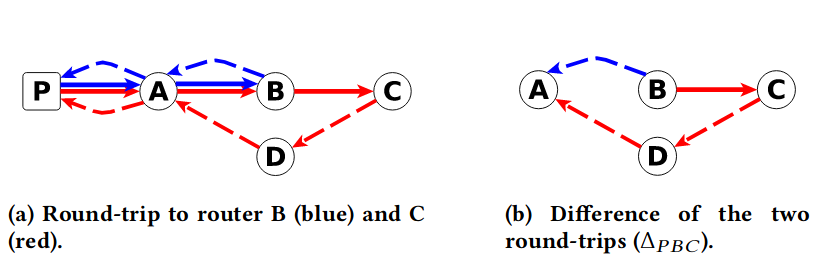
\includegraphics[width=0.7\linewidth]{illustrations/rtt-differ}
	\caption{}
	\label{fig:rtt-differ}
\end{figure}



\subsection{Le principe de la détection des changements des délais}

L'évolution du délai d'un lien est déduit  de l'évolution de son RTT différentiel. Reprenons la formule du RTT différentiel du lien BC :  $\delta_{BC}$ + $\varepsilon_{PBC}$. Supposons qu'on dispose d'un nombre $n$ de sondes Atlas P$_i$, $i$ $\in$ [$1$, $n$], telles que toutes les sondes ont un chemin de retour différent depuis B et depuis C.  En effet, les RTTs différentiels pour chacune des sondes Atlas $\Delta_{P{_i}BC}$ partagent la même composante $\delta_{BC}$, toutefois, ces RTTs ont des valeurs des  $\varepsilon_{P_{i}BC}$ indépendantes. L'indépendance de ces valeurs implique que la distribution $\Delta_{P_{i}BC}$ est estimé d'être stable au cours du temps si $\delta_{BC}$ est constant. Cependant, un changement significatif de la valeur de $\delta_{BC}$ influence les valeurs des RTTs différentiels. Dans ce cas, la distribution des RTTs différentiels change si $\delta_{BC}$ change. Enfin, les changements des délais sont déduits des changements des RTTs différentiels qu'on peut les quantifier.

La détection des anomalies des délais repose sur un théorème très important en statistiques, c'est le théorème  central limite (TCL). Ce théorème  annonce que si on a une suite de variables aléatoires $X_i$ indépendantes ayant la même espérance $µ$ et la même variance $\sigma^2$, la moyenne de ces variables aléatoires est une variable aléatoire qui suit une loi normale. 

%De manière générale, le théorème central limite explique la distribution des moyennes des échantillons. Ce théorème peut être appliquer aux différents lois. Par exemple la loi normale \footnote{Un exemple illustratif dans \ref{appendix:clt-exemple}.}, binomiale, etc. 


\subsection{Quelques précisions}

Le travail de référence \cite{DBLP:journals/corr/FontugneAPB16} implique principalement les mesures de type  traceroute. Deux catégories de mesures sont utilisées :

\begin{itemize}
	\item \textit{builtin} : ce sont les traceroutes effectués par toutes les sondes Atlas vers les instances des  $13$ serveurs DNS racines. Les traceroutes sont effectués chaque $30$ minutes. En pratique, certains serveurs racines DNS déploient l'anycast. Au moment de la réalisation du travail de référence\cite{DBLP:journals/corr/FontugneAPB16}, c'étaient des traceroutes vers $ 500 $ instances des serveurs DNS racines;
	\begin{tcolorbox}
		\textbf{DNS Anycast} est une solution   utilisée pour accélérer le fonctionnement  des serveurs DNS. Les serveurs DNS adoptant cette approche fournissent des temps de réponse plus courts, et ce partout dans le monde. Les requêtes en provenance de l'utilisateur sont redirigées vers un n\oe{}ud adéquat suivant un routage prédéfini. 
	\end{tcolorbox}
	
	\item \textit{anchoring} : ce sont les traceroutes effectués par environ $400$ sondes Atlas à destination de $189$ serveurs\footnote{Sondes Atlas ayant des fonctionnalités avancées.} et ce chaque $15$ minutes.
\end{itemize}

 Le tableau \ref{tab:dataset} reprend plus de détails  concernant les traceroutes analysés dans le cadre du travail de référence. Par exemple $2.8$ traceroutes effectués par des sondes Atlas ayant IPv4 comme adressage IP  ont été exploités dans le travail de référence, y inclus les deux autres méthodes. Ces traceroutes ont été effectués par $11.538$ sondes Atlas.

\begin{table}[H]
	\centering
	\begin{tabular}{|l|l|l|}
		\hline
		& \textbf{Nombre de traceroutes}& \textbf{Nombre de sondes Atlas }\\ \hline
		IPv4		&$ 2.8 $ billion & $ 11.538 $\\ \hline
		IPv6	&	$ 1.2 $ billion & $ 4.30 $ \\ \hline
	\end{tabular}
	\caption{Récapitulatif des traceroutes utilisés dans le travail de référence }
	\label{tab:dataset}
\end{table}

La méthode conçue pour la détection des changements des délais se base sur des fondements statistiques. Ces derniers sont capables de montrer leurs performances si la taille des échantillons des RTTs différentiel caractérisant un lien considérés est grande.   Afin de surveiller un grand nombre de liens sur Internet, il faut avoir un grand nombre de sondes Atlas avec une certaine diversité et  qui sont capables de collecter une quantité importante de données relatives aux performances des réseaux informatiques.



%L'étude des délais ne concerne pas  les adresses privées, ainsi, le suivi des délais ne concerne pas les réseaux privés.  De plus, ce  suivi  se base sur les requêtes de type traceroute, et traceroute reprend une partie de la topologie de l'Internet. En effet, les liens considérés sont ceux topologiques et ne sont pas  les liens physiques. 

\section{Description de la détection des anomalies dans liens}

La détection des anomalies dans les délais des liens passe par deux étapes principales. La première étape consiste à préparer les traceroutes. Quant à la deuxième étape, elle sert à calculer une référence pour ensuite comparer les nouvelles valeurs avec la valeur de référence. Cette  référence représente un intervalle de valeurs des RTTs différentiel ou un intervalle de confiance, toute nouvelle valeur de RTT est comparée avec l'intervalle de confiance et suite à cette comparaison, on caractérise le changement par rapport à la référence.  

\subsection{Vue générale du processus de la détection}

 La figure 	\ref{fig:process-detection} reprend le processus de la détection des anomalies dans le délais d'un lien. On distingue les deux étapes principales : la préparation des traceroutes et l'exploitation des données issues de l'étape de la préparation.  Dans chacune des étapes, on distingue un succession d'opérations. 
 
 L'objectif de l'étape de préparation des traceroutes est de traiter chaque traceroute, indépendamment des autres traceroutes. Toutefois, ces traceroutes sont regroupés par période, où une période est une durée marquée par un début et une fin. En ce qui concerne la deuxième étape, elle exploite les données de la première étape pour identifier les liens et les différents changements que l'ont subi.
  
\begin{figure}[H]
	\centering
	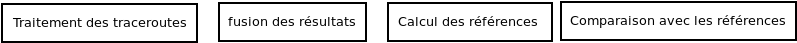
\includegraphics[width=1\linewidth]{illustrations/process-detection}
	\caption{Le processus de l'analyse des délais d'un lien.}
	\label{fig:process-detection}
\end{figure}

\subsection{Préparation des données}
 A l'étape de la préparation des traceroutes, on distingue trois opérations, premièrement c'est l'élimination des données inutiles dans un traceroute, voire le traceroute même s'il a échoué. Deuxièmement, c'est l'identification des liens topologiques et leurs caractérisation. Enfin, c'est la fusion des données si c'est nécessaire. 
 
\paragraph{L'élimination des données inutiles}~

  Un traceroute est sauvegardé en étant un object JSON, la figure \ref{annexe:traceroute-attributes} décrit les attributs qu'un traceroute peut contenir. D'une part, il y a les attributs obligatoires dont chaque traceroute doit révéler. D'autre part, il existe les attributs optionnels.  La conservation de tel ou tel attribut dépend de l'objectif pour lequel un traceroute est analysé.  

\paragraph{Vérification de la validation des données utiles}~

 Les données utiles dans l'analyse des délais doivent être validées suivant les objectifs spécifiques prédéfinis. Etant donné que l'analyse des délais ne concerne pas les réseaux informatiques privés, les adresses IP privées sont éliminées. Comme une sonde Atlas peut recevoir jusqu'à trois signaux différents pour un saut donné, chaque signal doit reprendre un RTT et une adresse IP source du signal. Le RTT doit être valide; positif non nul.
 
 
 \paragraph{Inférence des liens à partir d'un traceroute } ~
 
 
 La figure \ref{fig:links-inference} montre tous les  liens possibles qu'on peut retrouver en se basant sur l'approche adoptée dans le  travail de référence. Les routeurs impliqués dans le trafic lors d'une requête traceroute entre une  source et une destination forment les liens; chaque deux routeurs (R1, R2) consécutifs forment un lien topologique comme illustré dans la figure \ref{fig:links-inference}. Le RTT différentiel d'un lien est la différence entre le RTT de ces deux routeurs et la sonde Atlas (la source).
 
 
     \begin{landscape}
 	\begin{figure}[H]
 		\centering
 		\resizebox{20cm}{!}{
 			% Graphic for TeX using PGF
% Title: /home/bellafkih/Documents/2018-2019/memoire/rapport_memoire/dia/traceroute-exemple.dia
% Creator: Dia v0.97.3
% CreationDate: Fri Oct  5 16:42:09 2018
% For: bellafkih
% \usepackage{tikz}
% The following commands are not supported in PSTricks at present
% We define them conditionally, so when they are implemented,
% this pgf file will use them.
\ifx\du\undefined
  \newlength{\du}
\fi
\setlength{\du}{15\unitlength}
\begin{tikzpicture}
\pgftransformxscale{1.000000}
\pgftransformyscale{-1.000000}
\definecolor{dialinecolor}{rgb}{0.000000, 0.000000, 0.000000}
\pgfsetstrokecolor{dialinecolor}
\definecolor{dialinecolor}{rgb}{1.000000, 1.000000, 1.000000}
\pgfsetfillcolor{dialinecolor}
\pgfsetlinewidth{0.000000\du}
\pgfsetdash{}{0pt}
\pgfsetdash{}{0pt}
\pgfsetbuttcap
\pgfsetmiterjoin
\pgfsetlinewidth{0.000000\du}
\pgfsetbuttcap
\pgfsetmiterjoin
\pgfsetdash{}{0pt}
\definecolor{dialinecolor}{rgb}{0.027451, 0.486275, 0.682353}
\pgfsetfillcolor{dialinecolor}
\pgfpathmoveto{\pgfpoint{-6.844583\du}{14.308835\du}}
\pgfpathlineto{\pgfpoint{-6.846043\du}{14.338043\du}}
\pgfpathlineto{\pgfpoint{-6.853345\du}{14.367981\du}}
\pgfpathlineto{\pgfpoint{-6.863568\du}{14.396458\du}}
\pgfpathlineto{\pgfpoint{-6.878171\du}{14.424571\du}}
\pgfpathlineto{\pgfpoint{-6.897522\du}{14.452683\du}}
\pgfpathlineto{\pgfpoint{-6.919427\du}{14.480065\du}}
\pgfpathlineto{\pgfpoint{-6.946079\du}{14.507082\du}}
\pgfpathlineto{\pgfpoint{-6.976748\du}{14.533369\du}}
\pgfpathlineto{\pgfpoint{-7.009606\du}{14.558561\du}}
\pgfpathlineto{\pgfpoint{-7.046846\du}{14.583753\du}}
\pgfpathlineto{\pgfpoint{-7.087737\du}{14.607849\du}}
\pgfpathlineto{\pgfpoint{-7.131549\du}{14.631215\du}}
\pgfpathlineto{\pgfpoint{-7.177916\du}{14.653851\du}}
\pgfpathlineto{\pgfpoint{-7.228299\du}{14.675757\du}}
\pgfpathlineto{\pgfpoint{-7.281238\du}{14.696568\du}}
\pgfpathlineto{\pgfpoint{-7.336733\du}{14.716648\du}}
\pgfpathlineto{\pgfpoint{-7.394783\du}{14.735998\du}}
\pgfpathlineto{\pgfpoint{-7.455389\du}{14.753888\du}}
\pgfpathlineto{\pgfpoint{-7.519281\du}{14.771047\du}}
\pgfpathlineto{\pgfpoint{-7.584269\du}{14.787477\du}}
\pgfpathlineto{\pgfpoint{-7.652907\du}{14.802446\du}}
\pgfpathlineto{\pgfpoint{-7.723736\du}{14.815954\du}}
\pgfpathlineto{\pgfpoint{-7.795660\du}{14.828733\du}}
\pgfpathlineto{\pgfpoint{-7.870504\du}{14.840781\du}}
\pgfpathlineto{\pgfpoint{-7.946445\du}{14.850639\du}}
\pgfpathlineto{\pgfpoint{-8.024940\du}{14.859766\du}}
\pgfpathlineto{\pgfpoint{-8.104531\du}{14.867433\du}}
\pgfpathlineto{\pgfpoint{-8.185583\du}{14.874005\du}}
\pgfpathlineto{\pgfpoint{-8.268825\du}{14.879116\du}}
\pgfpathlineto{\pgfpoint{-8.352432\du}{14.882767\du}}
\pgfpathlineto{\pgfpoint{-8.437865\du}{14.884958\du}}
\pgfpathlineto{\pgfpoint{-8.524393\du}{14.885688\du}}
\pgfpathlineto{\pgfpoint{-8.610556\du}{14.884958\du}}
\pgfpathlineto{\pgfpoint{-8.696353\du}{14.882767\du}}
\pgfpathlineto{\pgfpoint{-8.779960\du}{14.879116\du}}
\pgfpathlineto{\pgfpoint{-8.862837\du}{14.874005\du}}
\pgfpathlineto{\pgfpoint{-8.944254\du}{14.867433\du}}
\pgfpathlineto{\pgfpoint{-9.023845\du}{14.859766\du}}
\pgfpathlineto{\pgfpoint{-9.101611\du}{14.850639\du}}
\pgfpathlineto{\pgfpoint{-9.178281\du}{14.840781\du}}
\pgfpathlineto{\pgfpoint{-9.252396\du}{14.828733\du}}
\pgfpathlineto{\pgfpoint{-9.325050\du}{14.815954\du}}
\pgfpathlineto{\pgfpoint{-9.395514\du}{14.802446\du}}
\pgfpathlineto{\pgfpoint{-9.464152\du}{14.787477\du}}
\pgfpathlineto{\pgfpoint{-9.529869\du}{14.771047\du}}
\pgfpathlineto{\pgfpoint{-9.593396\du}{14.753888\du}}
\pgfpathlineto{\pgfpoint{-9.654367\du}{14.735998\du}}
\pgfpathlineto{\pgfpoint{-9.712783\du}{14.716648\du}}
\pgfpathlineto{\pgfpoint{-9.767912\du}{14.696568\du}}
\pgfpathlineto{\pgfpoint{-9.820851\du}{14.675757\du}}
\pgfpathlineto{\pgfpoint{-9.870870\du}{14.653851\du}}
\pgfpathlineto{\pgfpoint{-9.917967\du}{14.631215\du}}
\pgfpathlineto{\pgfpoint{-9.961414\du}{14.607849\du}}
\pgfpathlineto{\pgfpoint{-10.002304\du}{14.583753\du}}
\pgfpathlineto{\pgfpoint{-10.039544\du}{14.558561\du}}
\pgfpathlineto{\pgfpoint{-10.072768\du}{14.533369\du}}
\pgfpathlineto{\pgfpoint{-10.103071\du}{14.507082\du}}
\pgfpathlineto{\pgfpoint{-10.129723\du}{14.480065\du}}
\pgfpathlineto{\pgfpoint{-10.151629\du}{14.452683\du}}
\pgfpathlineto{\pgfpoint{-10.170979\du}{14.424571\du}}
\pgfpathlineto{\pgfpoint{-10.185583\du}{14.396458\du}}
\pgfpathlineto{\pgfpoint{-10.196171\du}{14.367981\du}}
\pgfpathlineto{\pgfpoint{-10.203108\du}{14.338043\du}}
\pgfpathlineto{\pgfpoint{-10.204933\du}{14.308835\du}}
\pgfpathlineto{\pgfpoint{-10.203108\du}{14.278897\du}}
\pgfpathlineto{\pgfpoint{-10.196171\du}{14.249689\du}}
\pgfpathlineto{\pgfpoint{-10.185583\du}{14.220482\du}}
\pgfpathlineto{\pgfpoint{-10.170979\du}{14.192369\du}}
\pgfpathlineto{\pgfpoint{-10.151629\du}{14.164257\du}}
\pgfpathlineto{\pgfpoint{-10.129723\du}{14.136874\du}}
\pgfpathlineto{\pgfpoint{-10.103071\du}{14.110222\du}}
\pgfpathlineto{\pgfpoint{-10.072768\du}{14.083935\du}}
\pgfpathlineto{\pgfpoint{-10.039544\du}{14.058379\du}}
\pgfpathlineto{\pgfpoint{-10.002304\du}{14.033552\du}}
\pgfpathlineto{\pgfpoint{-9.961414\du}{14.009091\du}}
\pgfpathlineto{\pgfpoint{-9.917967\du}{13.985724\du}}
\pgfpathlineto{\pgfpoint{-9.870870\du}{13.963453\du}}
\pgfpathlineto{\pgfpoint{-9.820851\du}{13.941183\du}}
\pgfpathlineto{\pgfpoint{-9.767912\du}{13.920372\du}}
\pgfpathlineto{\pgfpoint{-9.712783\du}{13.900292\du}}
\pgfpathlineto{\pgfpoint{-9.654367\du}{13.881672\du}}
\pgfpathlineto{\pgfpoint{-9.593396\du}{13.862687\du}}
\pgfpathlineto{\pgfpoint{-9.529869\du}{13.845892\du}}
\pgfpathlineto{\pgfpoint{-9.464152\du}{13.830193\du}}
\pgfpathlineto{\pgfpoint{-9.395514\du}{13.814859\du}}
\pgfpathlineto{\pgfpoint{-9.325050\du}{13.800985\du}}
\pgfpathlineto{\pgfpoint{-9.252396\du}{13.787842\du}}
\pgfpathlineto{\pgfpoint{-9.178281\du}{13.776889\du}}
\pgfpathlineto{\pgfpoint{-9.101611\du}{13.766301\du}}
\pgfpathlineto{\pgfpoint{-9.023845\du}{13.756809\du}}
\pgfpathlineto{\pgfpoint{-8.944254\du}{13.749507\du}}
\pgfpathlineto{\pgfpoint{-8.862837\du}{13.742935\du}}
\pgfpathlineto{\pgfpoint{-8.779960\du}{13.737824\du}}
\pgfpathlineto{\pgfpoint{-8.696353\du}{13.734173\du}}
\pgfpathlineto{\pgfpoint{-8.610556\du}{13.732347\du}}
\pgfpathlineto{\pgfpoint{-8.524393\du}{13.731252\du}}
\pgfpathlineto{\pgfpoint{-8.437865\du}{13.732347\du}}
\pgfpathlineto{\pgfpoint{-8.352432\du}{13.734173\du}}
\pgfpathlineto{\pgfpoint{-8.268825\du}{13.737824\du}}
\pgfpathlineto{\pgfpoint{-8.185583\du}{13.742935\du}}
\pgfpathlineto{\pgfpoint{-8.104531\du}{13.749507\du}}
\pgfpathlineto{\pgfpoint{-8.024940\du}{13.756809\du}}
\pgfpathlineto{\pgfpoint{-7.946445\du}{13.766301\du}}
\pgfpathlineto{\pgfpoint{-7.870504\du}{13.776889\du}}
\pgfpathlineto{\pgfpoint{-7.795660\du}{13.787842\du}}
\pgfpathlineto{\pgfpoint{-7.723736\du}{13.800985\du}}
\pgfpathlineto{\pgfpoint{-7.652907\du}{13.814859\du}}
\pgfpathlineto{\pgfpoint{-7.584269\du}{13.830193\du}}
\pgfpathlineto{\pgfpoint{-7.519281\du}{13.845892\du}}
\pgfpathlineto{\pgfpoint{-7.455389\du}{13.862687\du}}
\pgfpathlineto{\pgfpoint{-7.394783\du}{13.881672\du}}
\pgfpathlineto{\pgfpoint{-7.336733\du}{13.900292\du}}
\pgfpathlineto{\pgfpoint{-7.281238\du}{13.920372\du}}
\pgfpathlineto{\pgfpoint{-7.228299\du}{13.941183\du}}
\pgfpathlineto{\pgfpoint{-7.177916\du}{13.963453\du}}
\pgfpathlineto{\pgfpoint{-7.131549\du}{13.985724\du}}
\pgfpathlineto{\pgfpoint{-7.087737\du}{14.009091\du}}
\pgfpathlineto{\pgfpoint{-7.046846\du}{14.033552\du}}
\pgfpathlineto{\pgfpoint{-7.009606\du}{14.058379\du}}
\pgfpathlineto{\pgfpoint{-6.976748\du}{14.083935\du}}
\pgfpathlineto{\pgfpoint{-6.946079\du}{14.110222\du}}
\pgfpathlineto{\pgfpoint{-6.919427\du}{14.136874\du}}
\pgfpathlineto{\pgfpoint{-6.897522\du}{14.164257\du}}
\pgfpathlineto{\pgfpoint{-6.878171\du}{14.192369\du}}
\pgfpathlineto{\pgfpoint{-6.863568\du}{14.220482\du}}
\pgfpathlineto{\pgfpoint{-6.853345\du}{14.249689\du}}
\pgfpathlineto{\pgfpoint{-6.846043\du}{14.278897\du}}
\pgfpathlineto{\pgfpoint{-6.844583\du}{14.308835\du}}
\pgfusepath{fill}
\pgfsetlinewidth{0.000000\du}
\pgfsetbuttcap
\pgfsetmiterjoin
\pgfsetdash{}{0pt}
\definecolor{dialinecolor}{rgb}{0.678431, 0.839216, 0.905882}
\pgfsetfillcolor{dialinecolor}
\pgfpathmoveto{\pgfpoint{-8.524393\du}{14.896276\du}}
\pgfpathlineto{\pgfpoint{-8.524393\du}{14.896276\du}}
\pgfpathlineto{\pgfpoint{-8.480946\du}{14.896276\du}}
\pgfpathlineto{\pgfpoint{-8.437500\du}{14.895545\du}}
\pgfpathlineto{\pgfpoint{-8.394418\du}{14.894450\du}}
\pgfpathlineto{\pgfpoint{-8.352432\du}{14.893355\du}}
\pgfpathlineto{\pgfpoint{-8.309716\du}{14.891529\du}}
\pgfpathlineto{\pgfpoint{-8.268095\du}{14.889339\du}}
\pgfpathlineto{\pgfpoint{-8.226474\du}{14.886783\du}}
\pgfpathlineto{\pgfpoint{-8.184853\du}{14.884593\du}}
\pgfpathlineto{\pgfpoint{-8.144327\du}{14.881672\du}}
\pgfpathlineto{\pgfpoint{-8.103436\du}{14.878021\du}}
\pgfpathlineto{\pgfpoint{-8.063641\du}{14.874005\du}}
\pgfpathlineto{\pgfpoint{-8.023480\du}{14.869989\du}}
\pgfpathlineto{\pgfpoint{-7.984780\du}{14.865607\du}}
\pgfpathlineto{\pgfpoint{-7.945349\du}{14.861226\du}}
\pgfpathlineto{\pgfpoint{-7.907379\du}{14.855750\du}}
\pgfpathlineto{\pgfpoint{-7.868314\du}{14.850639\du}}
\pgfpathlineto{\pgfpoint{-7.831074\du}{14.845162\du}}
\pgfpathlineto{\pgfpoint{-7.794199\du}{14.838955\du}}
\pgfpathlineto{\pgfpoint{-7.757690\du}{14.833114\du}}
\pgfpathlineto{\pgfpoint{-7.721180\du}{14.826542\du}}
\pgfpathlineto{\pgfpoint{-7.685765\du}{14.819605\du}}
\pgfpathlineto{\pgfpoint{-7.651081\du}{14.812668\du}}
\pgfpathlineto{\pgfpoint{-7.616397\du}{14.805001\du}}
\pgfpathlineto{\pgfpoint{-7.582443\du}{14.797334\du}}
\pgfpathlineto{\pgfpoint{-7.548854\du}{14.788937\du}}
\pgfpathlineto{\pgfpoint{-7.515995\du}{14.780905\du}}
\pgfpathlineto{\pgfpoint{-7.484232\du}{14.772873\du}}
\pgfpathlineto{\pgfpoint{-7.452834\du}{14.764111\du}}
\pgfpathlineto{\pgfpoint{-7.437500\du}{14.759364\du}}
\pgfpathlineto{\pgfpoint{-7.422166\du}{14.755348\du}}
\pgfpathlineto{\pgfpoint{-7.406101\du}{14.750602\du}}
\pgfpathlineto{\pgfpoint{-7.391497\du}{14.745856\du}}
\pgfpathlineto{\pgfpoint{-7.377259\du}{14.741110\du}}
\pgfpathlineto{\pgfpoint{-7.362290\du}{14.735998\du}}
\pgfpathlineto{\pgfpoint{-7.347321\du}{14.731252\du}}
\pgfpathlineto{\pgfpoint{-7.333447\du}{14.726506\du}}
\pgfpathlineto{\pgfpoint{-7.319208\du}{14.721394\du}}
\pgfpathlineto{\pgfpoint{-7.305335\du}{14.716648\du}}
\pgfpathlineto{\pgfpoint{-7.291096\du}{14.711172\du}}
\pgfpathlineto{\pgfpoint{-7.277952\du}{14.706790\du}}
\pgfpathlineto{\pgfpoint{-7.263714\du}{14.701314\du}}
\pgfpathlineto{\pgfpoint{-7.250570\du}{14.696203\du}}
\pgfpathlineto{\pgfpoint{-7.237427\du}{14.690726\du}}
\pgfpathlineto{\pgfpoint{-7.223918\du}{14.684885\du}}
\pgfpathlineto{\pgfpoint{-7.211140\du}{14.679773\du}}
\pgfpathlineto{\pgfpoint{-7.199092\du}{14.674297\du}}
\pgfpathlineto{\pgfpoint{-7.186313\du}{14.668455\du}}
\pgfpathlineto{\pgfpoint{-7.173900\du}{14.663344\du}}
\pgfpathlineto{\pgfpoint{-7.161487\du}{14.657502\du}}
\pgfpathlineto{\pgfpoint{-7.150169\du}{14.652026\du}}
\pgfpathlineto{\pgfpoint{-7.138120\du}{14.646184\du}}
\pgfpathlineto{\pgfpoint{-7.127167\du}{14.640343\du}}
\pgfpathlineto{\pgfpoint{-7.115484\du}{14.634501\du}}
\pgfpathlineto{\pgfpoint{-7.104166\du}{14.628660\du}}
\pgfpathlineto{\pgfpoint{-7.092848\du}{14.622818\du}}
\pgfpathlineto{\pgfpoint{-7.082261\du}{14.616612\du}}
\pgfpathlineto{\pgfpoint{-7.072403\du}{14.610770\du}}
\pgfpathlineto{\pgfpoint{-7.061815\du}{14.604928\du}}
\pgfpathlineto{\pgfpoint{-7.051592\du}{14.598357\du}}
\pgfpathlineto{\pgfpoint{-7.041735\du}{14.592515\du}}
\pgfpathlineto{\pgfpoint{-7.031877\du}{14.585943\du}}
\pgfpathlineto{\pgfpoint{-7.022750\du}{14.579737\du}}
\pgfpathlineto{\pgfpoint{-7.013622\du}{14.573165\du}}
\pgfpathlineto{\pgfpoint{-7.004130\du}{14.567323\du}}
\pgfpathlineto{\pgfpoint{-6.995368\du}{14.560752\du}}
\pgfpathlineto{\pgfpoint{-6.986240\du}{14.554545\du}}
\pgfpathlineto{\pgfpoint{-6.978208\du}{14.547973\du}}
\pgfpathlineto{\pgfpoint{-6.969446\du}{14.541036\du}}
\pgfpathlineto{\pgfpoint{-6.962144\du}{14.534465\du}}
\pgfpathlineto{\pgfpoint{-6.954112\du}{14.528258\du}}
\pgfpathlineto{\pgfpoint{-6.946079\du}{14.520956\du}}
\pgfpathlineto{\pgfpoint{-6.939508\du}{14.514750\du}}
\pgfpathlineto{\pgfpoint{-6.932206\du}{14.507813\du}}
\pgfpathlineto{\pgfpoint{-6.925634\du}{14.500511\du}}
\pgfpathlineto{\pgfpoint{-6.918697\du}{14.494304\du}}
\pgfpathlineto{\pgfpoint{-6.912125\du}{14.487367\du}}
\pgfpathlineto{\pgfpoint{-6.905919\du}{14.480065\du}}
\pgfpathlineto{\pgfpoint{-6.900077\du}{14.473128\du}}
\pgfpathlineto{\pgfpoint{-6.894601\du}{14.466192\du}}
\pgfpathlineto{\pgfpoint{-6.888759\du}{14.459255\du}}
\pgfpathlineto{\pgfpoint{-6.884013\du}{14.451953\du}}
\pgfpathlineto{\pgfpoint{-6.878537\du}{14.444651\du}}
\pgfpathlineto{\pgfpoint{-6.873790\du}{14.437349\du}}
\pgfpathlineto{\pgfpoint{-6.869409\du}{14.430412\du}}
\pgfpathlineto{\pgfpoint{-6.865393\du}{14.422745\du}}
\pgfpathlineto{\pgfpoint{-6.861377\du}{14.415808\du}}
\pgfpathlineto{\pgfpoint{-6.858091\du}{14.408141\du}}
\pgfpathlineto{\pgfpoint{-6.854075\du}{14.400474\du}}
\pgfpathlineto{\pgfpoint{-6.850789\du}{14.392807\du}}
\pgfpathlineto{\pgfpoint{-6.848234\du}{14.385505\du}}
\pgfpathlineto{\pgfpoint{-6.845313\du}{14.378203\du}}
\pgfpathlineto{\pgfpoint{-6.843487\du}{14.370901\du}}
\pgfpathlineto{\pgfpoint{-6.840566\du}{14.363234\du}}
\pgfpathlineto{\pgfpoint{-6.839471\du}{14.354837\du}}
\pgfpathlineto{\pgfpoint{-6.837281\du}{14.347170\du}}
\pgfpathlineto{\pgfpoint{-6.836185\du}{14.339868\du}}
\pgfpathlineto{\pgfpoint{-6.835455\du}{14.332201\du}}
\pgfpathlineto{\pgfpoint{-6.834725\du}{14.323804\du}}
\pgfpathlineto{\pgfpoint{-6.833995\du}{14.316502\du}}
\pgfpathlineto{\pgfpoint{-6.833995\du}{14.308835\du}}
\pgfpathlineto{\pgfpoint{-6.854075\du}{14.308835\du}}
\pgfpathlineto{\pgfpoint{-6.854805\du}{14.315772\du}}
\pgfpathlineto{\pgfpoint{-6.854805\du}{14.322709\du}}
\pgfpathlineto{\pgfpoint{-6.855170\du}{14.329645\du}}
\pgfpathlineto{\pgfpoint{-6.856996\du}{14.336947\du}}
\pgfpathlineto{\pgfpoint{-6.858091\du}{14.343884\du}}
\pgfpathlineto{\pgfpoint{-6.858821\du}{14.350821\du}}
\pgfpathlineto{\pgfpoint{-6.861012\du}{14.357758\du}}
\pgfpathlineto{\pgfpoint{-6.862472\du}{14.365060\du}}
\pgfpathlineto{\pgfpoint{-6.864663\du}{14.371266\du}}
\pgfpathlineto{\pgfpoint{-6.867219\du}{14.378203\du}}
\pgfpathlineto{\pgfpoint{-6.870139\du}{14.385505\du}}
\pgfpathlineto{\pgfpoint{-6.872695\du}{14.392442\du}}
\pgfpathlineto{\pgfpoint{-6.876711\du}{14.399379\du}}
\pgfpathlineto{\pgfpoint{-6.879632\du}{14.405951\du}}
\pgfpathlineto{\pgfpoint{-6.883648\du}{14.412888\du}}
\pgfpathlineto{\pgfpoint{-6.886569\du}{14.419459\du}}
\pgfpathlineto{\pgfpoint{-6.890950\du}{14.426396\du}}
\pgfpathlineto{\pgfpoint{-6.895331\du}{14.433333\du}}
\pgfpathlineto{\pgfpoint{-6.900077\du}{14.439905\du}}
\pgfpathlineto{\pgfpoint{-6.905189\du}{14.446111\du}}
\pgfpathlineto{\pgfpoint{-6.909935\du}{14.453413\du}}
\pgfpathlineto{\pgfpoint{-6.916142\du}{14.460350\du}}
\pgfpathlineto{\pgfpoint{-6.921618\du}{14.466557\du}}
\pgfpathlineto{\pgfpoint{-6.926729\du}{14.473128\du}}
\pgfpathlineto{\pgfpoint{-6.933301\du}{14.479700\du}}
\pgfpathlineto{\pgfpoint{-6.940238\du}{14.486637\du}}
\pgfpathlineto{\pgfpoint{-6.946079\du}{14.493209\du}}
\pgfpathlineto{\pgfpoint{-6.953381\du}{14.499415\du}}
\pgfpathlineto{\pgfpoint{-6.959953\du}{14.505987\du}}
\pgfpathlineto{\pgfpoint{-6.967620\du}{14.512194\du}}
\pgfpathlineto{\pgfpoint{-6.974922\du}{14.518766\du}}
\pgfpathlineto{\pgfpoint{-6.982954\du}{14.525337\du}}
\pgfpathlineto{\pgfpoint{-6.990621\du}{14.531544\du}}
\pgfpathlineto{\pgfpoint{-6.999384\du}{14.538116\du}}
\pgfpathlineto{\pgfpoint{-7.007781\du}{14.543957\du}}
\pgfpathlineto{\pgfpoint{-7.016543\du}{14.550529\du}}
\pgfpathlineto{\pgfpoint{-7.024575\du}{14.556736\du}}
\pgfpathlineto{\pgfpoint{-7.033338\du}{14.562577\du}}
\pgfpathlineto{\pgfpoint{-7.042830\du}{14.569149\du}}
\pgfpathlineto{\pgfpoint{-7.053053\du}{14.574990\du}}
\pgfpathlineto{\pgfpoint{-7.062180\du}{14.581562\du}}
\pgfpathlineto{\pgfpoint{-7.072403\du}{14.587404\du}}
\pgfpathlineto{\pgfpoint{-7.082261\du}{14.593245\du}}
\pgfpathlineto{\pgfpoint{-7.092118\du}{14.599087\du}}
\pgfpathlineto{\pgfpoint{-7.103071\du}{14.604928\du}}
\pgfpathlineto{\pgfpoint{-7.114024\du}{14.610770\du}}
\pgfpathlineto{\pgfpoint{-7.124247\du}{14.616612\du}}
\pgfpathlineto{\pgfpoint{-7.136295\du}{14.622453\du}}
\pgfpathlineto{\pgfpoint{-7.146883\du}{14.627564\du}}
\pgfpathlineto{\pgfpoint{-7.158931\du}{14.633406\du}}
\pgfpathlineto{\pgfpoint{-7.170249\du}{14.639248\du}}
\pgfpathlineto{\pgfpoint{-7.182662\du}{14.644724\du}}
\pgfpathlineto{\pgfpoint{-7.194710\du}{14.649835\du}}
\pgfpathlineto{\pgfpoint{-7.207124\du}{14.655677\du}}
\pgfpathlineto{\pgfpoint{-7.219172\du}{14.661153\du}}
\pgfpathlineto{\pgfpoint{-7.232315\du}{14.666265\du}}
\pgfpathlineto{\pgfpoint{-7.245094\du}{14.671376\du}}
\pgfpathlineto{\pgfpoint{-7.257872\du}{14.676852\du}}
\pgfpathlineto{\pgfpoint{-7.271016\du}{14.681964\du}}
\pgfpathlineto{\pgfpoint{-7.284524\du}{14.687440\du}}
\pgfpathlineto{\pgfpoint{-7.297668\du}{14.691821\du}}
\pgfpathlineto{\pgfpoint{-7.311906\du}{14.697298\du}}
\pgfpathlineto{\pgfpoint{-7.325780\du}{14.702044\du}}
\pgfpathlineto{\pgfpoint{-7.340019\du}{14.707156\du}}
\pgfpathlineto{\pgfpoint{-7.354623\du}{14.711902\du}}
\pgfpathlineto{\pgfpoint{-7.368496\du}{14.716648\du}}
\pgfpathlineto{\pgfpoint{-7.383100\du}{14.721394\du}}
\pgfpathlineto{\pgfpoint{-7.397339\du}{14.725775\du}}
\pgfpathlineto{\pgfpoint{-7.413038\du}{14.730522\du}}
\pgfpathlineto{\pgfpoint{-7.427277\du}{14.735268\du}}
\pgfpathlineto{\pgfpoint{-7.442976\du}{14.740014\du}}
\pgfpathlineto{\pgfpoint{-7.457945\du}{14.744030\du}}
\pgfpathlineto{\pgfpoint{-7.489343\du}{14.752793\du}}
\pgfpathlineto{\pgfpoint{-7.521472\du}{14.761190\du}}
\pgfpathlineto{\pgfpoint{-7.553600\du}{14.769222\du}}
\pgfpathlineto{\pgfpoint{-7.586824\du}{14.777254\du}}
\pgfpathlineto{\pgfpoint{-7.621143\du}{14.784921\du}}
\pgfpathlineto{\pgfpoint{-7.655097\du}{14.792223\du}}
\pgfpathlineto{\pgfpoint{-7.689782\du}{14.799160\du}}
\pgfpathlineto{\pgfpoint{-7.725561\du}{14.806097\du}}
\pgfpathlineto{\pgfpoint{-7.760975\du}{14.812668\du}}
\pgfpathlineto{\pgfpoint{-7.797850\du}{14.818875\du}}
\pgfpathlineto{\pgfpoint{-7.834360\du}{14.824717\du}}
\pgfpathlineto{\pgfpoint{-7.871600\du}{14.830558\du}}
\pgfpathlineto{\pgfpoint{-7.909205\du}{14.836035\du}}
\pgfpathlineto{\pgfpoint{-7.947905\du}{14.840781\du}}
\pgfpathlineto{\pgfpoint{-7.986605\du}{14.845162\du}}
\pgfpathlineto{\pgfpoint{-8.026036\du}{14.849908\du}}
\pgfpathlineto{\pgfpoint{-8.065101\du}{14.853559\du}}
\pgfpathlineto{\pgfpoint{-8.105262\du}{14.857575\du}}
\pgfpathlineto{\pgfpoint{-8.145422\du}{14.860496\du}}
\pgfpathlineto{\pgfpoint{-8.186678\du}{14.864147\du}}
\pgfpathlineto{\pgfpoint{-8.227569\du}{14.867068\du}}
\pgfpathlineto{\pgfpoint{-8.268825\du}{14.869258\du}}
\pgfpathlineto{\pgfpoint{-8.310446\du}{14.871084\du}}
\pgfpathlineto{\pgfpoint{-8.353162\du}{14.872909\du}}
\pgfpathlineto{\pgfpoint{-8.395879\du}{14.874005\du}}
\pgfpathlineto{\pgfpoint{-8.437865\du}{14.875100\du}}
\pgfpathlineto{\pgfpoint{-8.481311\du}{14.875100\du}}
\pgfpathlineto{\pgfpoint{-8.524393\du}{14.875830\du}}
\pgfpathlineto{\pgfpoint{-8.524393\du}{14.875830\du}}
\pgfpathlineto{\pgfpoint{-8.524393\du}{14.875830\du}}
\pgfpathlineto{\pgfpoint{-8.525123\du}{14.875830\du}}
\pgfpathlineto{\pgfpoint{-8.526948\du}{14.875830\du}}
\pgfpathlineto{\pgfpoint{-8.528044\du}{14.876195\du}}
\pgfpathlineto{\pgfpoint{-8.528774\du}{14.876195\du}}
\pgfpathlineto{\pgfpoint{-8.529139\du}{14.876925\du}}
\pgfpathlineto{\pgfpoint{-8.530599\du}{14.877291\du}}
\pgfpathlineto{\pgfpoint{-8.531330\du}{14.878021\du}}
\pgfpathlineto{\pgfpoint{-8.532060\du}{14.878751\du}}
\pgfpathlineto{\pgfpoint{-8.533155\du}{14.880576\du}}
\pgfpathlineto{\pgfpoint{-8.533885\du}{14.882037\du}}
\pgfpathlineto{\pgfpoint{-8.533885\du}{14.883862\du}}
\pgfpathlineto{\pgfpoint{-8.534615\du}{14.885688\du}}
\pgfpathlineto{\pgfpoint{-8.533885\du}{14.887878\du}}
\pgfpathlineto{\pgfpoint{-8.533885\du}{14.889704\du}}
\pgfpathlineto{\pgfpoint{-8.533155\du}{14.891529\du}}
\pgfpathlineto{\pgfpoint{-8.532060\du}{14.893355\du}}
\pgfpathlineto{\pgfpoint{-8.531330\du}{14.893720\du}}
\pgfpathlineto{\pgfpoint{-8.530599\du}{14.894450\du}}
\pgfpathlineto{\pgfpoint{-8.529139\du}{14.895180\du}}
\pgfpathlineto{\pgfpoint{-8.528774\du}{14.895545\du}}
\pgfpathlineto{\pgfpoint{-8.528044\du}{14.895545\du}}
\pgfpathlineto{\pgfpoint{-8.526948\du}{14.896276\du}}
\pgfpathlineto{\pgfpoint{-8.525123\du}{14.896276\du}}
\pgfpathlineto{\pgfpoint{-8.524393\du}{14.896276\du}}
\pgfusepath{fill}
\pgfsetbuttcap
\pgfsetmiterjoin
\pgfsetdash{}{0pt}
\definecolor{dialinecolor}{rgb}{0.678431, 0.839216, 0.905882}
\pgfsetfillcolor{dialinecolor}
\pgfpathmoveto{\pgfpoint{-10.215156\du}{14.308835\du}}
\pgfpathlineto{\pgfpoint{-10.215156\du}{14.308835\du}}
\pgfpathlineto{\pgfpoint{-10.215156\du}{14.316502\du}}
\pgfpathlineto{\pgfpoint{-10.214791\du}{14.323804\du}}
\pgfpathlineto{\pgfpoint{-10.214060\du}{14.332201\du}}
\pgfpathlineto{\pgfpoint{-10.212965\du}{14.339868\du}}
\pgfpathlineto{\pgfpoint{-10.211870\du}{14.347170\du}}
\pgfpathlineto{\pgfpoint{-10.210044\du}{14.354837\du}}
\pgfpathlineto{\pgfpoint{-10.208219\du}{14.363234\du}}
\pgfpathlineto{\pgfpoint{-10.206028\du}{14.370901\du}}
\pgfpathlineto{\pgfpoint{-10.203838\du}{14.378203\du}}
\pgfpathlineto{\pgfpoint{-10.201282\du}{14.385505\du}}
\pgfpathlineto{\pgfpoint{-10.198361\du}{14.392807\du}}
\pgfpathlineto{\pgfpoint{-10.194710\du}{14.400474\du}}
\pgfpathlineto{\pgfpoint{-10.191424\du}{14.408141\du}}
\pgfpathlineto{\pgfpoint{-10.187774\du}{14.415808\du}}
\pgfpathlineto{\pgfpoint{-10.183392\du}{14.422745\du}}
\pgfpathlineto{\pgfpoint{-10.179741\du}{14.430412\du}}
\pgfpathlineto{\pgfpoint{-10.174630\du}{14.437349\du}}
\pgfpathlineto{\pgfpoint{-10.170614\du}{14.444651\du}}
\pgfpathlineto{\pgfpoint{-10.165138\du}{14.451953\du}}
\pgfpathlineto{\pgfpoint{-10.160391\du}{14.459255\du}}
\pgfpathlineto{\pgfpoint{-10.154915\du}{14.466192\du}}
\pgfpathlineto{\pgfpoint{-10.149073\du}{14.473128\du}}
\pgfpathlineto{\pgfpoint{-10.143232\du}{14.480065\du}}
\pgfpathlineto{\pgfpoint{-10.137390\du}{14.487367\du}}
\pgfpathlineto{\pgfpoint{-10.130453\du}{14.494304\du}}
\pgfpathlineto{\pgfpoint{-10.123882\du}{14.500511\du}}
\pgfpathlineto{\pgfpoint{-10.116945\du}{14.507813\du}}
\pgfpathlineto{\pgfpoint{-10.110008\du}{14.514750\du}}
\pgfpathlineto{\pgfpoint{-10.103071\du}{14.520956\du}}
\pgfpathlineto{\pgfpoint{-10.094309\du}{14.528258\du}}
\pgfpathlineto{\pgfpoint{-10.087372\du}{14.534465\du}}
\pgfpathlineto{\pgfpoint{-10.079705\du}{14.541036\du}}
\pgfpathlineto{\pgfpoint{-10.070943\du}{14.547973\du}}
\pgfpathlineto{\pgfpoint{-10.062545\du}{14.554545\du}}
\pgfpathlineto{\pgfpoint{-10.053783\du}{14.560752\du}}
\pgfpathlineto{\pgfpoint{-10.045386\du}{14.567323\du}}
\pgfpathlineto{\pgfpoint{-10.035528\du}{14.573165\du}}
\pgfpathlineto{\pgfpoint{-10.026401\du}{14.579737\du}}
\pgfpathlineto{\pgfpoint{-10.016908\du}{14.585943\du}}
\pgfpathlineto{\pgfpoint{-10.007416\du}{14.592515\du}}
\pgfpathlineto{\pgfpoint{-9.997558\du}{14.598357\du}}
\pgfpathlineto{\pgfpoint{-9.987335\du}{14.604928\du}}
\pgfpathlineto{\pgfpoint{-9.977113\du}{14.610770\du}}
\pgfpathlineto{\pgfpoint{-9.966525\du}{14.616612\du}}
\pgfpathlineto{\pgfpoint{-9.956302\du}{14.622818\du}}
\pgfpathlineto{\pgfpoint{-9.945349\du}{14.628660\du}}
\pgfpathlineto{\pgfpoint{-9.933666\du}{14.634501\du}}
\pgfpathlineto{\pgfpoint{-9.922348\du}{14.640343\du}}
\pgfpathlineto{\pgfpoint{-9.910665\du}{14.646184\du}}
\pgfpathlineto{\pgfpoint{-9.899347\du}{14.652026\du}}
\pgfpathlineto{\pgfpoint{-9.887664\du}{14.657502\du}}
\pgfpathlineto{\pgfpoint{-9.875251\du}{14.663344\du}}
\pgfpathlineto{\pgfpoint{-9.863202\du}{14.668455\du}}
\pgfpathlineto{\pgfpoint{-9.850059\du}{14.674297\du}}
\pgfpathlineto{\pgfpoint{-9.838011\du}{14.679773\du}}
\pgfpathlineto{\pgfpoint{-9.825232\du}{14.684885\du}}
\pgfpathlineto{\pgfpoint{-9.811359\du}{14.690726\du}}
\pgfpathlineto{\pgfpoint{-9.798945\du}{14.696203\du}}
\pgfpathlineto{\pgfpoint{-9.785802\du}{14.701314\du}}
\pgfpathlineto{\pgfpoint{-9.771563\du}{14.706790\du}}
\pgfpathlineto{\pgfpoint{-9.758420\du}{14.711172\du}}
\pgfpathlineto{\pgfpoint{-9.744181\du}{14.716648\du}}
\pgfpathlineto{\pgfpoint{-9.730307\du}{14.721394\du}}
\pgfpathlineto{\pgfpoint{-9.715703\du}{14.726506\du}}
\pgfpathlineto{\pgfpoint{-9.701830\du}{14.731252\du}}
\pgfpathlineto{\pgfpoint{-9.686131\du}{14.735998\du}}
\pgfpathlineto{\pgfpoint{-9.672257\du}{14.741110\du}}
\pgfpathlineto{\pgfpoint{-9.657653\du}{14.745856\du}}
\pgfpathlineto{\pgfpoint{-9.642319\du}{14.750602\du}}
\pgfpathlineto{\pgfpoint{-9.626620\du}{14.755348\du}}
\pgfpathlineto{\pgfpoint{-9.611651\du}{14.759364\du}}
\pgfpathlineto{\pgfpoint{-9.595952\du}{14.764111\du}}
\pgfpathlineto{\pgfpoint{-9.564188\du}{14.772873\du}}
\pgfpathlineto{\pgfpoint{-9.532425\du}{14.780905\du}}
\pgfpathlineto{\pgfpoint{-9.499201\du}{14.788937\du}}
\pgfpathlineto{\pgfpoint{-9.466707\du}{14.797334\du}}
\pgfpathlineto{\pgfpoint{-9.432023\du}{14.805001\du}}
\pgfpathlineto{\pgfpoint{-9.397704\du}{14.812668\du}}
\pgfpathlineto{\pgfpoint{-9.363020\du}{14.819605\du}}
\pgfpathlineto{\pgfpoint{-9.327240\du}{14.826542\du}}
\pgfpathlineto{\pgfpoint{-9.291096\du}{14.833114\du}}
\pgfpathlineto{\pgfpoint{-9.254586\du}{14.838955\du}}
\pgfpathlineto{\pgfpoint{-9.217346\du}{14.845162\du}}
\pgfpathlineto{\pgfpoint{-9.179741\du}{14.850639\du}}
\pgfpathlineto{\pgfpoint{-9.141771\du}{14.855750\du}}
\pgfpathlineto{\pgfpoint{-9.103071\du}{14.861226\du}}
\pgfpathlineto{\pgfpoint{-9.064371\du}{14.865607\du}}
\pgfpathlineto{\pgfpoint{-9.025305\du}{14.869989\du}}
\pgfpathlineto{\pgfpoint{-8.985145\du}{14.874005\du}}
\pgfpathlineto{\pgfpoint{-8.945349\du}{14.878021\du}}
\pgfpathlineto{\pgfpoint{-8.904458\du}{14.881672\du}}
\pgfpathlineto{\pgfpoint{-8.863568\du}{14.884593\du}}
\pgfpathlineto{\pgfpoint{-8.822312\du}{14.886783\du}}
\pgfpathlineto{\pgfpoint{-8.780326\du}{14.889339\du}}
\pgfpathlineto{\pgfpoint{-8.738705\du}{14.891529\du}}
\pgfpathlineto{\pgfpoint{-8.696353\du}{14.893355\du}}
\pgfpathlineto{\pgfpoint{-8.654367\du}{14.894450\du}}
\pgfpathlineto{\pgfpoint{-8.610921\du}{14.895545\du}}
\pgfpathlineto{\pgfpoint{-8.568204\du}{14.896276\du}}
\pgfpathlineto{\pgfpoint{-8.524393\du}{14.896276\du}}
\pgfpathlineto{\pgfpoint{-8.524393\du}{14.875830\du}}
\pgfpathlineto{\pgfpoint{-8.567109\du}{14.875100\du}}
\pgfpathlineto{\pgfpoint{-8.610556\du}{14.875100\du}}
\pgfpathlineto{\pgfpoint{-8.652907\du}{14.874005\du}}
\pgfpathlineto{\pgfpoint{-8.695623\du}{14.872909\du}}
\pgfpathlineto{\pgfpoint{-8.737974\du}{14.871084\du}}
\pgfpathlineto{\pgfpoint{-8.779960\du}{14.869258\du}}
\pgfpathlineto{\pgfpoint{-8.820851\du}{14.867068\du}}
\pgfpathlineto{\pgfpoint{-8.862107\du}{14.864147\du}}
\pgfpathlineto{\pgfpoint{-8.902998\du}{14.860496\du}}
\pgfpathlineto{\pgfpoint{-8.943159\du}{14.857575\du}}
\pgfpathlineto{\pgfpoint{-8.982954\du}{14.853559\du}}
\pgfpathlineto{\pgfpoint{-9.022385\du}{14.849908\du}}
\pgfpathlineto{\pgfpoint{-9.061815\du}{14.845162\du}}
\pgfpathlineto{\pgfpoint{-9.100880\du}{14.840781\du}}
\pgfpathlineto{\pgfpoint{-9.139216\du}{14.836035\du}}
\pgfpathlineto{\pgfpoint{-9.176821\du}{14.830558\du}}
\pgfpathlineto{\pgfpoint{-9.214060\du}{14.824717\du}}
\pgfpathlineto{\pgfpoint{-9.250570\du}{14.818875\du}}
\pgfpathlineto{\pgfpoint{-9.287810\du}{14.812668\du}}
\pgfpathlineto{\pgfpoint{-9.322859\du}{14.806097\du}}
\pgfpathlineto{\pgfpoint{-9.359004\du}{14.799160\du}}
\pgfpathlineto{\pgfpoint{-9.393688\du}{14.792223\du}}
\pgfpathlineto{\pgfpoint{-9.428007\du}{14.784921\du}}
\pgfpathlineto{\pgfpoint{-9.461961\du}{14.777254\du}}
\pgfpathlineto{\pgfpoint{-9.495185\du}{14.769222\du}}
\pgfpathlineto{\pgfpoint{-9.526583\du}{14.761190\du}}
\pgfpathlineto{\pgfpoint{-9.559077\du}{14.752793\du}}
\pgfpathlineto{\pgfpoint{-9.590110\du}{14.744030\du}}
\pgfpathlineto{\pgfpoint{-9.605809\du}{14.740014\du}}
\pgfpathlineto{\pgfpoint{-9.621508\du}{14.735268\du}}
\pgfpathlineto{\pgfpoint{-9.636112\du}{14.730522\du}}
\pgfpathlineto{\pgfpoint{-9.651081\du}{14.725775\du}}
\pgfpathlineto{\pgfpoint{-9.666415\du}{14.721394\du}}
\pgfpathlineto{\pgfpoint{-9.680654\du}{14.716648\du}}
\pgfpathlineto{\pgfpoint{-9.694893\du}{14.711902\du}}
\pgfpathlineto{\pgfpoint{-9.709132\du}{14.707156\du}}
\pgfpathlineto{\pgfpoint{-9.723370\du}{14.702044\du}}
\pgfpathlineto{\pgfpoint{-9.737244\du}{14.697298\du}}
\pgfpathlineto{\pgfpoint{-9.751118\du}{14.691821\du}}
\pgfpathlineto{\pgfpoint{-9.764626\du}{14.687440\du}}
\pgfpathlineto{\pgfpoint{-9.778135\du}{14.681964\du}}
\pgfpathlineto{\pgfpoint{-9.790913\du}{14.676852\du}}
\pgfpathlineto{\pgfpoint{-9.804422\du}{14.671376\du}}
\pgfpathlineto{\pgfpoint{-9.817200\du}{14.666265\du}}
\pgfpathlineto{\pgfpoint{-9.829614\du}{14.661153\du}}
\pgfpathlineto{\pgfpoint{-9.842757\du}{14.655677\du}}
\pgfpathlineto{\pgfpoint{-9.854805\du}{14.649835\du}}
\pgfpathlineto{\pgfpoint{-9.866123\du}{14.644724\du}}
\pgfpathlineto{\pgfpoint{-9.878902\du}{14.639248\du}}
\pgfpathlineto{\pgfpoint{-9.890585\du}{14.633406\du}}
\pgfpathlineto{\pgfpoint{-9.902268\du}{14.627564\du}}
\pgfpathlineto{\pgfpoint{-9.913221\du}{14.622453\du}}
\pgfpathlineto{\pgfpoint{-9.924904\du}{14.616612\du}}
\pgfpathlineto{\pgfpoint{-9.934761\du}{14.610770\du}}
\pgfpathlineto{\pgfpoint{-9.946079\du}{14.604928\du}}
\pgfpathlineto{\pgfpoint{-9.956667\du}{14.599087\du}}
\pgfpathlineto{\pgfpoint{-9.966525\du}{14.593245\du}}
\pgfpathlineto{\pgfpoint{-9.977113\du}{14.587404\du}}
\pgfpathlineto{\pgfpoint{-9.986970\du}{14.581562\du}}
\pgfpathlineto{\pgfpoint{-9.996463\du}{14.574990\du}}
\pgfpathlineto{\pgfpoint{-10.006320\du}{14.569149\du}}
\pgfpathlineto{\pgfpoint{-10.015448\du}{14.562577\du}}
\pgfpathlineto{\pgfpoint{-10.023845\du}{14.556736\du}}
\pgfpathlineto{\pgfpoint{-10.032607\du}{14.550529\du}}
\pgfpathlineto{\pgfpoint{-10.041735\du}{14.543957\du}}
\pgfpathlineto{\pgfpoint{-10.050497\du}{14.538116\du}}
\pgfpathlineto{\pgfpoint{-10.058894\du}{14.531544\du}}
\pgfpathlineto{\pgfpoint{-10.066196\du}{14.525337\du}}
\pgfpathlineto{\pgfpoint{-10.074228\du}{14.518766\du}}
\pgfpathlineto{\pgfpoint{-10.081895\du}{14.512194\du}}
\pgfpathlineto{\pgfpoint{-10.088832\du}{14.505987\du}}
\pgfpathlineto{\pgfpoint{-10.096134\du}{14.499415\du}}
\pgfpathlineto{\pgfpoint{-10.103071\du}{14.493209\du}}
\pgfpathlineto{\pgfpoint{-10.109278\du}{14.486637\du}}
\pgfpathlineto{\pgfpoint{-10.115849\du}{14.479700\du}}
\pgfpathlineto{\pgfpoint{-10.121691\du}{14.473128\du}}
\pgfpathlineto{\pgfpoint{-10.127898\du}{14.466557\du}}
\pgfpathlineto{\pgfpoint{-10.133009\du}{14.460350\du}}
\pgfpathlineto{\pgfpoint{-10.139216\du}{14.453413\du}}
\pgfpathlineto{\pgfpoint{-10.143597\du}{14.446842\du}}
\pgfpathlineto{\pgfpoint{-10.149073\du}{14.439905\du}}
\pgfpathlineto{\pgfpoint{-10.153454\du}{14.433333\du}}
\pgfpathlineto{\pgfpoint{-10.157836\du}{14.426396\du}}
\pgfpathlineto{\pgfpoint{-10.162217\du}{14.419459\du}}
\pgfpathlineto{\pgfpoint{-10.165503\du}{14.412888\du}}
\pgfpathlineto{\pgfpoint{-10.169519\du}{14.405951\du}}
\pgfpathlineto{\pgfpoint{-10.173535\du}{14.399379\du}}
\pgfpathlineto{\pgfpoint{-10.176456\du}{14.392442\du}}
\pgfpathlineto{\pgfpoint{-10.179011\du}{14.385505\du}}
\pgfpathlineto{\pgfpoint{-10.182297\du}{14.378203\du}}
\pgfpathlineto{\pgfpoint{-10.184488\du}{14.371266\du}}
\pgfpathlineto{\pgfpoint{-10.186678\du}{14.365060\du}}
\pgfpathlineto{\pgfpoint{-10.188139\du}{14.357758\du}}
\pgfpathlineto{\pgfpoint{-10.190329\du}{14.350821\du}}
\pgfpathlineto{\pgfpoint{-10.191424\du}{14.343884\du}}
\pgfpathlineto{\pgfpoint{-10.192520\du}{14.336947\du}}
\pgfpathlineto{\pgfpoint{-10.193980\du}{14.329645\du}}
\pgfpathlineto{\pgfpoint{-10.194345\du}{14.322709\du}}
\pgfpathlineto{\pgfpoint{-10.194345\du}{14.315772\du}}
\pgfpathlineto{\pgfpoint{-10.194710\du}{14.308835\du}}
\pgfpathlineto{\pgfpoint{-10.194710\du}{14.308835\du}}
\pgfpathlineto{\pgfpoint{-10.194710\du}{14.308835\du}}
\pgfpathlineto{\pgfpoint{-10.194710\du}{14.307009\du}}
\pgfpathlineto{\pgfpoint{-10.194710\du}{14.306279\du}}
\pgfpathlineto{\pgfpoint{-10.195075\du}{14.305184\du}}
\pgfpathlineto{\pgfpoint{-10.195075\du}{14.304089\du}}
\pgfpathlineto{\pgfpoint{-10.196171\du}{14.303359\du}}
\pgfpathlineto{\pgfpoint{-10.196536\du}{14.302263\du}}
\pgfpathlineto{\pgfpoint{-10.196901\du}{14.301533\du}}
\pgfpathlineto{\pgfpoint{-10.197996\du}{14.301168\du}}
\pgfpathlineto{\pgfpoint{-10.199457\du}{14.300073\du}}
\pgfpathlineto{\pgfpoint{-10.201282\du}{14.298612\du}}
\pgfpathlineto{\pgfpoint{-10.203108\du}{14.298247\du}}
\pgfpathlineto{\pgfpoint{-10.204933\du}{14.298247\du}}
\pgfpathlineto{\pgfpoint{-10.207124\du}{14.298247\du}}
\pgfpathlineto{\pgfpoint{-10.208584\du}{14.298612\du}}
\pgfpathlineto{\pgfpoint{-10.210775\du}{14.300073\du}}
\pgfpathlineto{\pgfpoint{-10.212600\du}{14.301168\du}}
\pgfpathlineto{\pgfpoint{-10.212965\du}{14.301533\du}}
\pgfpathlineto{\pgfpoint{-10.213330\du}{14.302263\du}}
\pgfpathlineto{\pgfpoint{-10.214060\du}{14.303359\du}}
\pgfpathlineto{\pgfpoint{-10.214791\du}{14.304089\du}}
\pgfpathlineto{\pgfpoint{-10.214791\du}{14.305184\du}}
\pgfpathlineto{\pgfpoint{-10.215156\du}{14.306279\du}}
\pgfpathlineto{\pgfpoint{-10.215156\du}{14.307009\du}}
\pgfpathlineto{\pgfpoint{-10.215156\du}{14.308835\du}}
\pgfusepath{fill}
\pgfsetbuttcap
\pgfsetmiterjoin
\pgfsetdash{}{0pt}
\definecolor{dialinecolor}{rgb}{0.678431, 0.839216, 0.905882}
\pgfsetfillcolor{dialinecolor}
\pgfpathmoveto{\pgfpoint{-8.524393\du}{13.721394\du}}
\pgfpathlineto{\pgfpoint{-8.524393\du}{13.721394\du}}
\pgfpathlineto{\pgfpoint{-8.568204\du}{13.721394\du}}
\pgfpathlineto{\pgfpoint{-8.610921\du}{13.721759\du}}
\pgfpathlineto{\pgfpoint{-8.654367\du}{13.722855\du}}
\pgfpathlineto{\pgfpoint{-8.696353\du}{13.724315\du}}
\pgfpathlineto{\pgfpoint{-8.738705\du}{13.725775\du}}
\pgfpathlineto{\pgfpoint{-8.780326\du}{13.727601\du}}
\pgfpathlineto{\pgfpoint{-8.822312\du}{13.730157\du}}
\pgfpathlineto{\pgfpoint{-8.863568\du}{13.733077\du}}
\pgfpathlineto{\pgfpoint{-8.904458\du}{13.735998\du}}
\pgfpathlineto{\pgfpoint{-8.945349\du}{13.738919\du}}
\pgfpathlineto{\pgfpoint{-8.985145\du}{13.742935\du}}
\pgfpathlineto{\pgfpoint{-9.025305\du}{13.746951\du}}
\pgfpathlineto{\pgfpoint{-9.064371\du}{13.751697\du}}
\pgfpathlineto{\pgfpoint{-9.103071\du}{13.756444\du}}
\pgfpathlineto{\pgfpoint{-9.141771\du}{13.761190\du}}
\pgfpathlineto{\pgfpoint{-9.179741\du}{13.766301\du}}
\pgfpathlineto{\pgfpoint{-9.217346\du}{13.772143\du}}
\pgfpathlineto{\pgfpoint{-9.254586\du}{13.777984\du}}
\pgfpathlineto{\pgfpoint{-9.291096\du}{13.784556\du}}
\pgfpathlineto{\pgfpoint{-9.327240\du}{13.790763\du}}
\pgfpathlineto{\pgfpoint{-9.363020\du}{13.798065\du}}
\pgfpathlineto{\pgfpoint{-9.397704\du}{13.805001\du}}
\pgfpathlineto{\pgfpoint{-9.432023\du}{13.811938\du}}
\pgfpathlineto{\pgfpoint{-9.466707\du}{13.819970\du}}
\pgfpathlineto{\pgfpoint{-9.499201\du}{13.827637\du}}
\pgfpathlineto{\pgfpoint{-9.532425\du}{13.836035\du}}
\pgfpathlineto{\pgfpoint{-9.564188\du}{13.844797\du}}
\pgfpathlineto{\pgfpoint{-9.595952\du}{13.853559\du}}
\pgfpathlineto{\pgfpoint{-9.626620\du}{13.862322\du}}
\pgfpathlineto{\pgfpoint{-9.657653\du}{13.871814\du}}
\pgfpathlineto{\pgfpoint{-9.672257\du}{13.876195\du}}
\pgfpathlineto{\pgfpoint{-9.686131\du}{13.880942\du}}
\pgfpathlineto{\pgfpoint{-9.701830\du}{13.885688\du}}
\pgfpathlineto{\pgfpoint{-9.715703\du}{13.890799\du}}
\pgfpathlineto{\pgfpoint{-9.730307\du}{13.895545\du}}
\pgfpathlineto{\pgfpoint{-9.744181\du}{13.901022\du}}
\pgfpathlineto{\pgfpoint{-9.758420\du}{13.905403\du}}
\pgfpathlineto{\pgfpoint{-9.771563\du}{13.910879\du}}
\pgfpathlineto{\pgfpoint{-9.785802\du}{13.915991\du}}
\pgfpathlineto{\pgfpoint{-9.798945\du}{13.921467\du}}
\pgfpathlineto{\pgfpoint{-9.811359\du}{13.926579\du}}
\pgfpathlineto{\pgfpoint{-9.825232\du}{13.932055\du}}
\pgfpathlineto{\pgfpoint{-9.838011\du}{13.937166\du}}
\pgfpathlineto{\pgfpoint{-9.850059\du}{13.942278\du}}
\pgfpathlineto{\pgfpoint{-9.863202\du}{13.948119\du}}
\pgfpathlineto{\pgfpoint{-9.875251\du}{13.954326\du}}
\pgfpathlineto{\pgfpoint{-9.887664\du}{13.959437\du}}
\pgfpathlineto{\pgfpoint{-9.899347\du}{13.965279\du}}
\pgfpathlineto{\pgfpoint{-9.910665\du}{13.971120\du}}
\pgfpathlineto{\pgfpoint{-9.922348\du}{13.976962\du}}
\pgfpathlineto{\pgfpoint{-9.933666\du}{13.982804\du}}
\pgfpathlineto{\pgfpoint{-9.945349\du}{13.987915\du}}
\pgfpathlineto{\pgfpoint{-9.956302\du}{13.994487\du}}
\pgfpathlineto{\pgfpoint{-9.966525\du}{14.000328\du}}
\pgfpathlineto{\pgfpoint{-9.977113\du}{14.006170\du}}
\pgfpathlineto{\pgfpoint{-9.987335\du}{14.012011\du}}
\pgfpathlineto{\pgfpoint{-9.997558\du}{14.018583\du}}
\pgfpathlineto{\pgfpoint{-10.007416\du}{14.024790\du}}
\pgfpathlineto{\pgfpoint{-10.016908\du}{14.030631\du}}
\pgfpathlineto{\pgfpoint{-10.026401\du}{14.037203\du}}
\pgfpathlineto{\pgfpoint{-10.035528\du}{14.043775\du}}
\pgfpathlineto{\pgfpoint{-10.045386\du}{14.049981\du}}
\pgfpathlineto{\pgfpoint{-10.053783\du}{14.056553\du}}
\pgfpathlineto{\pgfpoint{-10.062545\du}{14.063125\du}}
\pgfpathlineto{\pgfpoint{-10.070943\du}{14.069331\du}}
\pgfpathlineto{\pgfpoint{-10.079705\du}{14.075903\du}}
\pgfpathlineto{\pgfpoint{-10.087372\du}{14.082840\du}}
\pgfpathlineto{\pgfpoint{-10.094309\du}{14.089412\du}}
\pgfpathlineto{\pgfpoint{-10.103071\du}{14.095618\du}}
\pgfpathlineto{\pgfpoint{-10.110008\du}{14.102920\du}}
\pgfpathlineto{\pgfpoint{-10.116945\du}{14.109127\du}}
\pgfpathlineto{\pgfpoint{-10.123882\du}{14.116064\du}}
\pgfpathlineto{\pgfpoint{-10.130453\du}{14.123366\du}}
\pgfpathlineto{\pgfpoint{-10.137390\du}{14.129572\du}}
\pgfpathlineto{\pgfpoint{-10.143232\du}{14.136874\du}}
\pgfpathlineto{\pgfpoint{-10.149073\du}{14.143811\du}}
\pgfpathlineto{\pgfpoint{-10.154915\du}{14.151478\du}}
\pgfpathlineto{\pgfpoint{-10.160391\du}{14.158415\du}}
\pgfpathlineto{\pgfpoint{-10.165138\du}{14.165352\du}}
\pgfpathlineto{\pgfpoint{-10.170614\du}{14.172289\du}}
\pgfpathlineto{\pgfpoint{-10.174630\du}{14.179591\du}}
\pgfpathlineto{\pgfpoint{-10.179741\du}{14.186893\du}}
\pgfpathlineto{\pgfpoint{-10.183392\du}{14.194195\du}}
\pgfpathlineto{\pgfpoint{-10.187774\du}{14.201497\du}}
\pgfpathlineto{\pgfpoint{-10.191424\du}{14.209164\du}}
\pgfpathlineto{\pgfpoint{-10.194710\du}{14.216831\du}}
\pgfpathlineto{\pgfpoint{-10.198361\du}{14.223767\du}}
\pgfpathlineto{\pgfpoint{-10.201282\du}{14.231434\du}}
\pgfpathlineto{\pgfpoint{-10.203838\du}{14.239101\du}}
\pgfpathlineto{\pgfpoint{-10.206028\du}{14.246769\du}}
\pgfpathlineto{\pgfpoint{-10.208219\du}{14.254436\du}}
\pgfpathlineto{\pgfpoint{-10.210044\du}{14.261737\du}}
\pgfpathlineto{\pgfpoint{-10.211870\du}{14.269405\du}}
\pgfpathlineto{\pgfpoint{-10.212965\du}{14.277072\du}}
\pgfpathlineto{\pgfpoint{-10.214060\du}{14.285469\du}}
\pgfpathlineto{\pgfpoint{-10.214791\du}{14.292771\du}}
\pgfpathlineto{\pgfpoint{-10.215156\du}{14.300438\du}}
\pgfpathlineto{\pgfpoint{-10.215156\du}{14.308835\du}}
\pgfpathlineto{\pgfpoint{-10.194710\du}{14.308835\du}}
\pgfpathlineto{\pgfpoint{-10.194345\du}{14.301533\du}}
\pgfpathlineto{\pgfpoint{-10.194345\du}{14.294596\du}}
\pgfpathlineto{\pgfpoint{-10.193980\du}{14.287659\du}}
\pgfpathlineto{\pgfpoint{-10.192520\du}{14.279992\du}}
\pgfpathlineto{\pgfpoint{-10.191424\du}{14.273786\du}}
\pgfpathlineto{\pgfpoint{-10.190329\du}{14.266484\du}}
\pgfpathlineto{\pgfpoint{-10.188139\du}{14.259547\du}}
\pgfpathlineto{\pgfpoint{-10.186678\du}{14.252610\du}}
\pgfpathlineto{\pgfpoint{-10.184488\du}{14.245673\du}}
\pgfpathlineto{\pgfpoint{-10.182297\du}{14.238371\du}}
\pgfpathlineto{\pgfpoint{-10.179011\du}{14.232165\du}}
\pgfpathlineto{\pgfpoint{-10.176456\du}{14.225228\du}}
\pgfpathlineto{\pgfpoint{-10.173535\du}{14.217926\du}}
\pgfpathlineto{\pgfpoint{-10.169519\du}{14.210989\du}}
\pgfpathlineto{\pgfpoint{-10.165503\du}{14.204052\du}}
\pgfpathlineto{\pgfpoint{-10.162217\du}{14.197480\du}}
\pgfpathlineto{\pgfpoint{-10.158201\du}{14.190544\du}}
\pgfpathlineto{\pgfpoint{-10.153454\du}{14.183972\du}}
\pgfpathlineto{\pgfpoint{-10.149073\du}{14.177035\du}}
\pgfpathlineto{\pgfpoint{-10.143597\du}{14.170463\du}}
\pgfpathlineto{\pgfpoint{-10.139216\du}{14.164257\du}}
\pgfpathlineto{\pgfpoint{-10.133009\du}{14.157320\du}}
\pgfpathlineto{\pgfpoint{-10.127898\du}{14.150748\du}}
\pgfpathlineto{\pgfpoint{-10.121691\du}{14.143811\du}}
\pgfpathlineto{\pgfpoint{-10.115849\du}{14.137239\du}}
\pgfpathlineto{\pgfpoint{-10.109278\du}{14.131033\du}}
\pgfpathlineto{\pgfpoint{-10.103071\du}{14.124461\du}}
\pgfpathlineto{\pgfpoint{-10.096134\du}{14.117524\du}}
\pgfpathlineto{\pgfpoint{-10.088832\du}{14.111683\du}}
\pgfpathlineto{\pgfpoint{-10.081895\du}{14.104381\du}}
\pgfpathlineto{\pgfpoint{-10.074228\du}{14.098174\du}}
\pgfpathlineto{\pgfpoint{-10.066196\du}{14.092333\du}}
\pgfpathlineto{\pgfpoint{-10.058894\du}{14.085761\du}}
\pgfpathlineto{\pgfpoint{-10.050497\du}{14.079189\du}}
\pgfpathlineto{\pgfpoint{-10.041735\du}{14.072982\du}}
\pgfpathlineto{\pgfpoint{-10.032607\du}{14.066411\du}}
\pgfpathlineto{\pgfpoint{-10.023845\du}{14.060569\du}}
\pgfpathlineto{\pgfpoint{-10.015448\du}{14.054363\du}}
\pgfpathlineto{\pgfpoint{-10.006320\du}{14.048521\du}}
\pgfpathlineto{\pgfpoint{-9.996463\du}{14.041949\du}}
\pgfpathlineto{\pgfpoint{-9.986970\du}{14.036108\du}}
\pgfpathlineto{\pgfpoint{-9.977113\du}{14.030266\du}}
\pgfpathlineto{\pgfpoint{-9.966525\du}{14.024425\du}}
\pgfpathlineto{\pgfpoint{-9.956667\du}{14.018583\du}}
\pgfpathlineto{\pgfpoint{-9.946079\du}{14.012011\du}}
\pgfpathlineto{\pgfpoint{-9.934761\du}{14.006900\du}}
\pgfpathlineto{\pgfpoint{-9.924904\du}{14.001058\du}}
\pgfpathlineto{\pgfpoint{-9.913221\du}{13.995217\du}}
\pgfpathlineto{\pgfpoint{-9.902268\du}{13.989375\du}}
\pgfpathlineto{\pgfpoint{-9.890585\du}{13.983534\du}}
\pgfpathlineto{\pgfpoint{-9.878902\du}{13.978057\du}}
\pgfpathlineto{\pgfpoint{-9.866123\du}{13.972946\du}}
\pgfpathlineto{\pgfpoint{-9.854805\du}{13.967104\du}}
\pgfpathlineto{\pgfpoint{-9.842757\du}{13.961628\du}}
\pgfpathlineto{\pgfpoint{-9.829614\du}{13.956517\du}}
\pgfpathlineto{\pgfpoint{-9.817200\du}{13.951040\du}}
\pgfpathlineto{\pgfpoint{-9.804422\du}{13.945929\du}}
\pgfpathlineto{\pgfpoint{-9.790913\du}{13.940087\du}}
\pgfpathlineto{\pgfpoint{-9.778135\du}{13.935341\du}}
\pgfpathlineto{\pgfpoint{-9.764626\du}{13.930230\du}}
\pgfpathlineto{\pgfpoint{-9.751118\du}{13.924753\du}}
\pgfpathlineto{\pgfpoint{-9.737244\du}{13.920372\du}}
\pgfpathlineto{\pgfpoint{-9.723370\du}{13.914896\du}}
\pgfpathlineto{\pgfpoint{-9.709132\du}{13.910149\du}}
\pgfpathlineto{\pgfpoint{-9.694893\du}{13.905403\du}}
\pgfpathlineto{\pgfpoint{-9.680654\du}{13.900292\du}}
\pgfpathlineto{\pgfpoint{-9.666415\du}{13.895545\du}}
\pgfpathlineto{\pgfpoint{-9.651081\du}{13.890799\du}}
\pgfpathlineto{\pgfpoint{-9.621508\du}{13.882037\du}}
\pgfpathlineto{\pgfpoint{-9.590110\du}{13.872909\du}}
\pgfpathlineto{\pgfpoint{-9.559077\du}{13.864512\du}}
\pgfpathlineto{\pgfpoint{-9.526583\du}{13.855750\du}}
\pgfpathlineto{\pgfpoint{-9.495185\du}{13.847718\du}}
\pgfpathlineto{\pgfpoint{-9.461961\du}{13.840051\du}}
\pgfpathlineto{\pgfpoint{-9.428007\du}{13.832384\du}}
\pgfpathlineto{\pgfpoint{-9.393688\du}{13.824717\du}}
\pgfpathlineto{\pgfpoint{-9.359004\du}{13.817780\du}}
\pgfpathlineto{\pgfpoint{-9.322859\du}{13.810843\du}}
\pgfpathlineto{\pgfpoint{-9.287810\du}{13.805001\du}}
\pgfpathlineto{\pgfpoint{-9.250570\du}{13.798430\du}}
\pgfpathlineto{\pgfpoint{-9.214060\du}{13.792588\du}}
\pgfpathlineto{\pgfpoint{-9.176821\du}{13.786747\du}}
\pgfpathlineto{\pgfpoint{-9.139216\du}{13.781635\du}}
\pgfpathlineto{\pgfpoint{-9.100880\du}{13.776159\du}}
\pgfpathlineto{\pgfpoint{-9.061815\du}{13.771413\du}}
\pgfpathlineto{\pgfpoint{-9.022385\du}{13.767396\du}}
\pgfpathlineto{\pgfpoint{-8.982954\du}{13.763380\du}}
\pgfpathlineto{\pgfpoint{-8.943159\du}{13.759729\du}}
\pgfpathlineto{\pgfpoint{-8.902998\du}{13.756444\du}}
\pgfpathlineto{\pgfpoint{-8.862107\du}{13.753523\du}}
\pgfpathlineto{\pgfpoint{-8.820851\du}{13.750602\du}}
\pgfpathlineto{\pgfpoint{-8.779960\du}{13.748046\du}}
\pgfpathlineto{\pgfpoint{-8.737974\du}{13.745856\du}}
\pgfpathlineto{\pgfpoint{-8.695623\du}{13.744760\du}}
\pgfpathlineto{\pgfpoint{-8.652907\du}{13.742935\du}}
\pgfpathlineto{\pgfpoint{-8.610556\du}{13.742205\du}}
\pgfpathlineto{\pgfpoint{-8.567109\du}{13.741840\du}}
\pgfpathlineto{\pgfpoint{-8.524393\du}{13.741840\du}}
\pgfpathlineto{\pgfpoint{-8.524393\du}{13.741840\du}}
\pgfpathlineto{\pgfpoint{-8.524393\du}{13.741840\du}}
\pgfpathlineto{\pgfpoint{-8.523297\du}{13.741110\du}}
\pgfpathlineto{\pgfpoint{-8.522202\du}{13.741110\du}}
\pgfpathlineto{\pgfpoint{-8.520742\du}{13.741110\du}}
\pgfpathlineto{\pgfpoint{-8.519646\du}{13.740744\du}}
\pgfpathlineto{\pgfpoint{-8.519281\du}{13.740014\du}}
\pgfpathlineto{\pgfpoint{-8.518186\du}{13.740014\du}}
\pgfpathlineto{\pgfpoint{-8.517456\du}{13.738919\du}}
\pgfpathlineto{\pgfpoint{-8.516361\du}{13.738189\du}}
\pgfpathlineto{\pgfpoint{-8.515265\du}{13.737093\du}}
\pgfpathlineto{\pgfpoint{-8.514535\du}{13.735268\du}}
\pgfpathlineto{\pgfpoint{-8.514535\du}{13.733077\du}}
\pgfpathlineto{\pgfpoint{-8.513805\du}{13.731252\du}}
\pgfpathlineto{\pgfpoint{-8.514535\du}{13.729426\du}}
\pgfpathlineto{\pgfpoint{-8.514535\du}{13.727601\du}}
\pgfpathlineto{\pgfpoint{-8.515265\du}{13.725775\du}}
\pgfpathlineto{\pgfpoint{-8.516361\du}{13.724315\du}}
\pgfpathlineto{\pgfpoint{-8.517456\du}{13.723585\du}}
\pgfpathlineto{\pgfpoint{-8.518186\du}{13.722855\du}}
\pgfpathlineto{\pgfpoint{-8.519281\du}{13.722490\du}}
\pgfpathlineto{\pgfpoint{-8.519646\du}{13.721759\du}}
\pgfpathlineto{\pgfpoint{-8.520742\du}{13.721394\du}}
\pgfpathlineto{\pgfpoint{-8.522202\du}{13.721394\du}}
\pgfpathlineto{\pgfpoint{-8.523297\du}{13.721394\du}}
\pgfpathlineto{\pgfpoint{-8.524393\du}{13.721394\du}}
\pgfusepath{fill}
\pgfsetbuttcap
\pgfsetmiterjoin
\pgfsetdash{}{0pt}
\definecolor{dialinecolor}{rgb}{0.678431, 0.839216, 0.905882}
\pgfsetfillcolor{dialinecolor}
\pgfpathmoveto{\pgfpoint{-6.833995\du}{14.308835\du}}
\pgfpathlineto{\pgfpoint{-6.833995\du}{14.300438\du}}
\pgfpathlineto{\pgfpoint{-6.834725\du}{14.292771\du}}
\pgfpathlineto{\pgfpoint{-6.835455\du}{14.285469\du}}
\pgfpathlineto{\pgfpoint{-6.836185\du}{14.277072\du}}
\pgfpathlineto{\pgfpoint{-6.837281\du}{14.269405\du}}
\pgfpathlineto{\pgfpoint{-6.839471\du}{14.261737\du}}
\pgfpathlineto{\pgfpoint{-6.840566\du}{14.254436\du}}
\pgfpathlineto{\pgfpoint{-6.843487\du}{14.246769\du}}
\pgfpathlineto{\pgfpoint{-6.845313\du}{14.239101\du}}
\pgfpathlineto{\pgfpoint{-6.848234\du}{14.231434\du}}
\pgfpathlineto{\pgfpoint{-6.850789\du}{14.223767\du}}
\pgfpathlineto{\pgfpoint{-6.854075\du}{14.216831\du}}
\pgfpathlineto{\pgfpoint{-6.858091\du}{14.209164\du}}
\pgfpathlineto{\pgfpoint{-6.861377\du}{14.201497\du}}
\pgfpathlineto{\pgfpoint{-6.865393\du}{14.194195\du}}
\pgfpathlineto{\pgfpoint{-6.869409\du}{14.186893\du}}
\pgfpathlineto{\pgfpoint{-6.873790\du}{14.179591\du}}
\pgfpathlineto{\pgfpoint{-6.878537\du}{14.172289\du}}
\pgfpathlineto{\pgfpoint{-6.884013\du}{14.165352\du}}
\pgfpathlineto{\pgfpoint{-6.888759\du}{14.158415\du}}
\pgfpathlineto{\pgfpoint{-6.894601\du}{14.150748\du}}
\pgfpathlineto{\pgfpoint{-6.900077\du}{14.143811\du}}
\pgfpathlineto{\pgfpoint{-6.905919\du}{14.136874\du}}
\pgfpathlineto{\pgfpoint{-6.912125\du}{14.129572\du}}
\pgfpathlineto{\pgfpoint{-6.918697\du}{14.123366\du}}
\pgfpathlineto{\pgfpoint{-6.925634\du}{14.116064\du}}
\pgfpathlineto{\pgfpoint{-6.932206\du}{14.109127\du}}
\pgfpathlineto{\pgfpoint{-6.939508\du}{14.102920\du}}
\pgfpathlineto{\pgfpoint{-6.946079\du}{14.095618\du}}
\pgfpathlineto{\pgfpoint{-6.954112\du}{14.089412\du}}
\pgfpathlineto{\pgfpoint{-6.962144\du}{14.082840\du}}
\pgfpathlineto{\pgfpoint{-6.969446\du}{14.075903\du}}
\pgfpathlineto{\pgfpoint{-6.978208\du}{14.069331\du}}
\pgfpathlineto{\pgfpoint{-6.986240\du}{14.063125\du}}
\pgfpathlineto{\pgfpoint{-6.995368\du}{14.056553\du}}
\pgfpathlineto{\pgfpoint{-7.004130\du}{14.049981\du}}
\pgfpathlineto{\pgfpoint{-7.013622\du}{14.043775\du}}
\pgfpathlineto{\pgfpoint{-7.022750\du}{14.037203\du}}
\pgfpathlineto{\pgfpoint{-7.031877\du}{14.030631\du}}
\pgfpathlineto{\pgfpoint{-7.041735\du}{14.024790\du}}
\pgfpathlineto{\pgfpoint{-7.051592\du}{14.018583\du}}
\pgfpathlineto{\pgfpoint{-7.061815\du}{14.012011\du}}
\pgfpathlineto{\pgfpoint{-7.072403\du}{14.006170\du}}
\pgfpathlineto{\pgfpoint{-7.082261\du}{14.000328\du}}
\pgfpathlineto{\pgfpoint{-7.092848\du}{13.994487\du}}
\pgfpathlineto{\pgfpoint{-7.104166\du}{13.987915\du}}
\pgfpathlineto{\pgfpoint{-7.115484\du}{13.982804\du}}
\pgfpathlineto{\pgfpoint{-7.127167\du}{13.976962\du}}
\pgfpathlineto{\pgfpoint{-7.138120\du}{13.971120\du}}
\pgfpathlineto{\pgfpoint{-7.150169\du}{13.965279\du}}
\pgfpathlineto{\pgfpoint{-7.161487\du}{13.959437\du}}
\pgfpathlineto{\pgfpoint{-7.173900\du}{13.954326\du}}
\pgfpathlineto{\pgfpoint{-7.186313\du}{13.948119\du}}
\pgfpathlineto{\pgfpoint{-7.199092\du}{13.942278\du}}
\pgfpathlineto{\pgfpoint{-7.211140\du}{13.937166\du}}
\pgfpathlineto{\pgfpoint{-7.223918\du}{13.932055\du}}
\pgfpathlineto{\pgfpoint{-7.237427\du}{13.926579\du}}
\pgfpathlineto{\pgfpoint{-7.250570\du}{13.921467\du}}
\pgfpathlineto{\pgfpoint{-7.263714\du}{13.915991\du}}
\pgfpathlineto{\pgfpoint{-7.277952\du}{13.910879\du}}
\pgfpathlineto{\pgfpoint{-7.291096\du}{13.905403\du}}
\pgfpathlineto{\pgfpoint{-7.305335\du}{13.901022\du}}
\pgfpathlineto{\pgfpoint{-7.319208\du}{13.895545\du}}
\pgfpathlineto{\pgfpoint{-7.333447\du}{13.890799\du}}
\pgfpathlineto{\pgfpoint{-7.347321\du}{13.885688\du}}
\pgfpathlineto{\pgfpoint{-7.362290\du}{13.880942\du}}
\pgfpathlineto{\pgfpoint{-7.377259\du}{13.876195\du}}
\pgfpathlineto{\pgfpoint{-7.391497\du}{13.871814\du}}
\pgfpathlineto{\pgfpoint{-7.422166\du}{13.862322\du}}
\pgfpathlineto{\pgfpoint{-7.452834\du}{13.853559\du}}
\pgfpathlineto{\pgfpoint{-7.484232\du}{13.844797\du}}
\pgfpathlineto{\pgfpoint{-7.515995\du}{13.836035\du}}
\pgfpathlineto{\pgfpoint{-7.548854\du}{13.827637\du}}
\pgfpathlineto{\pgfpoint{-7.582443\du}{13.819970\du}}
\pgfpathlineto{\pgfpoint{-7.616397\du}{13.811938\du}}
\pgfpathlineto{\pgfpoint{-7.651081\du}{13.805001\du}}
\pgfpathlineto{\pgfpoint{-7.685765\du}{13.798065\du}}
\pgfpathlineto{\pgfpoint{-7.721180\du}{13.790763\du}}
\pgfpathlineto{\pgfpoint{-7.757690\du}{13.784556\du}}
\pgfpathlineto{\pgfpoint{-7.794199\du}{13.777984\du}}
\pgfpathlineto{\pgfpoint{-7.831074\du}{13.772143\du}}
\pgfpathlineto{\pgfpoint{-7.868314\du}{13.766301\du}}
\pgfpathlineto{\pgfpoint{-7.907379\du}{13.761190\du}}
\pgfpathlineto{\pgfpoint{-7.945349\du}{13.756444\du}}
\pgfpathlineto{\pgfpoint{-7.984780\du}{13.751697\du}}
\pgfpathlineto{\pgfpoint{-8.023480\du}{13.746951\du}}
\pgfpathlineto{\pgfpoint{-8.063641\du}{13.742935\du}}
\pgfpathlineto{\pgfpoint{-8.103436\du}{13.738919\du}}
\pgfpathlineto{\pgfpoint{-8.144327\du}{13.735998\du}}
\pgfpathlineto{\pgfpoint{-8.184853\du}{13.733077\du}}
\pgfpathlineto{\pgfpoint{-8.226474\du}{13.730157\du}}
\pgfpathlineto{\pgfpoint{-8.268095\du}{13.727601\du}}
\pgfpathlineto{\pgfpoint{-8.309716\du}{13.725775\du}}
\pgfpathlineto{\pgfpoint{-8.352432\du}{13.724315\du}}
\pgfpathlineto{\pgfpoint{-8.394418\du}{13.722855\du}}
\pgfpathlineto{\pgfpoint{-8.437500\du}{13.721759\du}}
\pgfpathlineto{\pgfpoint{-8.480946\du}{13.721394\du}}
\pgfpathlineto{\pgfpoint{-8.524393\du}{13.721394\du}}
\pgfpathlineto{\pgfpoint{-8.524393\du}{13.741840\du}}
\pgfpathlineto{\pgfpoint{-8.481311\du}{13.741840\du}}
\pgfpathlineto{\pgfpoint{-8.437865\du}{13.742205\du}}
\pgfpathlineto{\pgfpoint{-8.395879\du}{13.742935\du}}
\pgfpathlineto{\pgfpoint{-8.353162\du}{13.744760\du}}
\pgfpathlineto{\pgfpoint{-8.310446\du}{13.745856\du}}
\pgfpathlineto{\pgfpoint{-8.268825\du}{13.748046\du}}
\pgfpathlineto{\pgfpoint{-8.227569\du}{13.750602\du}}
\pgfpathlineto{\pgfpoint{-8.186678\du}{13.753523\du}}
\pgfpathlineto{\pgfpoint{-8.145422\du}{13.756444\du}}
\pgfpathlineto{\pgfpoint{-8.105262\du}{13.759729\du}}
\pgfpathlineto{\pgfpoint{-8.065101\du}{13.763380\du}}
\pgfpathlineto{\pgfpoint{-8.026036\du}{13.767396\du}}
\pgfpathlineto{\pgfpoint{-7.986605\du}{13.771413\du}}
\pgfpathlineto{\pgfpoint{-7.947905\du}{13.776159\du}}
\pgfpathlineto{\pgfpoint{-7.909205\du}{13.781635\du}}
\pgfpathlineto{\pgfpoint{-7.871600\du}{13.786747\du}}
\pgfpathlineto{\pgfpoint{-7.834360\du}{13.792588\du}}
\pgfpathlineto{\pgfpoint{-7.797850\du}{13.798430\du}}
\pgfpathlineto{\pgfpoint{-7.760975\du}{13.805001\du}}
\pgfpathlineto{\pgfpoint{-7.725561\du}{13.810843\du}}
\pgfpathlineto{\pgfpoint{-7.689782\du}{13.817780\du}}
\pgfpathlineto{\pgfpoint{-7.655097\du}{13.824717\du}}
\pgfpathlineto{\pgfpoint{-7.621143\du}{13.832384\du}}
\pgfpathlineto{\pgfpoint{-7.586824\du}{13.840051\du}}
\pgfpathlineto{\pgfpoint{-7.553600\du}{13.847718\du}}
\pgfpathlineto{\pgfpoint{-7.521472\du}{13.855750\du}}
\pgfpathlineto{\pgfpoint{-7.489343\du}{13.864512\du}}
\pgfpathlineto{\pgfpoint{-7.457945\du}{13.872909\du}}
\pgfpathlineto{\pgfpoint{-7.427277\du}{13.882037\du}}
\pgfpathlineto{\pgfpoint{-7.397339\du}{13.890799\du}}
\pgfpathlineto{\pgfpoint{-7.383100\du}{13.895545\du}}
\pgfpathlineto{\pgfpoint{-7.368496\du}{13.900292\du}}
\pgfpathlineto{\pgfpoint{-7.354623\du}{13.905403\du}}
\pgfpathlineto{\pgfpoint{-7.340019\du}{13.910149\du}}
\pgfpathlineto{\pgfpoint{-7.325780\du}{13.914896\du}}
\pgfpathlineto{\pgfpoint{-7.311906\du}{13.920372\du}}
\pgfpathlineto{\pgfpoint{-7.297668\du}{13.924753\du}}
\pgfpathlineto{\pgfpoint{-7.284524\du}{13.930230\du}}
\pgfpathlineto{\pgfpoint{-7.271016\du}{13.935341\du}}
\pgfpathlineto{\pgfpoint{-7.257872\du}{13.940087\du}}
\pgfpathlineto{\pgfpoint{-7.245094\du}{13.945929\du}}
\pgfpathlineto{\pgfpoint{-7.232315\du}{13.951040\du}}
\pgfpathlineto{\pgfpoint{-7.219172\du}{13.956517\du}}
\pgfpathlineto{\pgfpoint{-7.207124\du}{13.961628\du}}
\pgfpathlineto{\pgfpoint{-7.194710\du}{13.967104\du}}
\pgfpathlineto{\pgfpoint{-7.182662\du}{13.972946\du}}
\pgfpathlineto{\pgfpoint{-7.170249\du}{13.978057\du}}
\pgfpathlineto{\pgfpoint{-7.158931\du}{13.983534\du}}
\pgfpathlineto{\pgfpoint{-7.146883\du}{13.989375\du}}
\pgfpathlineto{\pgfpoint{-7.136295\du}{13.995217\du}}
\pgfpathlineto{\pgfpoint{-7.124247\du}{14.001058\du}}
\pgfpathlineto{\pgfpoint{-7.114024\du}{14.006900\du}}
\pgfpathlineto{\pgfpoint{-7.103071\du}{14.012011\du}}
\pgfpathlineto{\pgfpoint{-7.092118\du}{14.018583\du}}
\pgfpathlineto{\pgfpoint{-7.082261\du}{14.024425\du}}
\pgfpathlineto{\pgfpoint{-7.072403\du}{14.030266\du}}
\pgfpathlineto{\pgfpoint{-7.062180\du}{14.036108\du}}
\pgfpathlineto{\pgfpoint{-7.053053\du}{14.041949\du}}
\pgfpathlineto{\pgfpoint{-7.042830\du}{14.048521\du}}
\pgfpathlineto{\pgfpoint{-7.033338\du}{14.054363\du}}
\pgfpathlineto{\pgfpoint{-7.024575\du}{14.060569\du}}
\pgfpathlineto{\pgfpoint{-7.016543\du}{14.066411\du}}
\pgfpathlineto{\pgfpoint{-7.007781\du}{14.072982\du}}
\pgfpathlineto{\pgfpoint{-6.999384\du}{14.079189\du}}
\pgfpathlineto{\pgfpoint{-6.990621\du}{14.085761\du}}
\pgfpathlineto{\pgfpoint{-6.982954\du}{14.092333\du}}
\pgfpathlineto{\pgfpoint{-6.974922\du}{14.098174\du}}
\pgfpathlineto{\pgfpoint{-6.967620\du}{14.104381\du}}
\pgfpathlineto{\pgfpoint{-6.959953\du}{14.111683\du}}
\pgfpathlineto{\pgfpoint{-6.953381\du}{14.117524\du}}
\pgfpathlineto{\pgfpoint{-6.946079\du}{14.124461\du}}
\pgfpathlineto{\pgfpoint{-6.940238\du}{14.131033\du}}
\pgfpathlineto{\pgfpoint{-6.933301\du}{14.137239\du}}
\pgfpathlineto{\pgfpoint{-6.926729\du}{14.143811\du}}
\pgfpathlineto{\pgfpoint{-6.921618\du}{14.150748\du}}
\pgfpathlineto{\pgfpoint{-6.916142\du}{14.157320\du}}
\pgfpathlineto{\pgfpoint{-6.909935\du}{14.164257\du}}
\pgfpathlineto{\pgfpoint{-6.905189\du}{14.170463\du}}
\pgfpathlineto{\pgfpoint{-6.900077\du}{14.177035\du}}
\pgfpathlineto{\pgfpoint{-6.895331\du}{14.183972\du}}
\pgfpathlineto{\pgfpoint{-6.890950\du}{14.190544\du}}
\pgfpathlineto{\pgfpoint{-6.886569\du}{14.197480\du}}
\pgfpathlineto{\pgfpoint{-6.883648\du}{14.204052\du}}
\pgfpathlineto{\pgfpoint{-6.879632\du}{14.210989\du}}
\pgfpathlineto{\pgfpoint{-6.876711\du}{14.217926\du}}
\pgfpathlineto{\pgfpoint{-6.872695\du}{14.225228\du}}
\pgfpathlineto{\pgfpoint{-6.870139\du}{14.231434\du}}
\pgfpathlineto{\pgfpoint{-6.867219\du}{14.238371\du}}
\pgfpathlineto{\pgfpoint{-6.864663\du}{14.245673\du}}
\pgfpathlineto{\pgfpoint{-6.862472\du}{14.252610\du}}
\pgfpathlineto{\pgfpoint{-6.861012\du}{14.259547\du}}
\pgfpathlineto{\pgfpoint{-6.858821\du}{14.266484\du}}
\pgfpathlineto{\pgfpoint{-6.858091\du}{14.273786\du}}
\pgfpathlineto{\pgfpoint{-6.856996\du}{14.279992\du}}
\pgfpathlineto{\pgfpoint{-6.855170\du}{14.287659\du}}
\pgfpathlineto{\pgfpoint{-6.854805\du}{14.294596\du}}
\pgfpathlineto{\pgfpoint{-6.854805\du}{14.301533\du}}
\pgfpathlineto{\pgfpoint{-6.854075\du}{14.308835\du}}
\pgfpathlineto{\pgfpoint{-6.833995\du}{14.308835\du}}
\pgfusepath{fill}
\pgfsetbuttcap
\pgfsetmiterjoin
\pgfsetdash{}{0pt}
\definecolor{dialinecolor}{rgb}{0.027451, 0.486275, 0.682353}
\pgfsetfillcolor{dialinecolor}
\pgfpathmoveto{\pgfpoint{-10.210044\du}{13.499415\du}}
\pgfpathlineto{\pgfpoint{-10.210044\du}{14.323804\du}}
\pgfpathlineto{\pgfpoint{-6.844583\du}{14.323804\du}}
\pgfpathlineto{\pgfpoint{-6.843852\du}{13.500146\du}}
\pgfpathlineto{\pgfpoint{-10.210044\du}{13.499415\du}}
\pgfusepath{fill}
\pgfsetbuttcap
\pgfsetmiterjoin
\pgfsetdash{}{0pt}
\definecolor{dialinecolor}{rgb}{0.235294, 0.686275, 0.894118}
\pgfsetfillcolor{dialinecolor}
\pgfpathmoveto{\pgfpoint{-6.844583\du}{13.483716\du}}
\pgfpathlineto{\pgfpoint{-6.846043\du}{13.513654\du}}
\pgfpathlineto{\pgfpoint{-6.853345\du}{13.542862\du}}
\pgfpathlineto{\pgfpoint{-6.863568\du}{13.572070\du}}
\pgfpathlineto{\pgfpoint{-6.878171\du}{13.600182\du}}
\pgfpathlineto{\pgfpoint{-6.897522\du}{13.628295\du}}
\pgfpathlineto{\pgfpoint{-6.919427\du}{13.655677\du}}
\pgfpathlineto{\pgfpoint{-6.946079\du}{13.681964\du}}
\pgfpathlineto{\pgfpoint{-6.976748\du}{13.708251\du}}
\pgfpathlineto{\pgfpoint{-7.009606\du}{13.734173\du}}
\pgfpathlineto{\pgfpoint{-7.046846\du}{13.759364\du}}
\pgfpathlineto{\pgfpoint{-7.087737\du}{13.783461\du}}
\pgfpathlineto{\pgfpoint{-7.131549\du}{13.806827\du}}
\pgfpathlineto{\pgfpoint{-7.177916\du}{13.829098\du}}
\pgfpathlineto{\pgfpoint{-7.228299\du}{13.851004\du}}
\pgfpathlineto{\pgfpoint{-7.281238\du}{13.872179\du}}
\pgfpathlineto{\pgfpoint{-7.336733\du}{13.892260\du}}
\pgfpathlineto{\pgfpoint{-7.394783\du}{13.910879\du}}
\pgfpathlineto{\pgfpoint{-7.455389\du}{13.929499\du}}
\pgfpathlineto{\pgfpoint{-7.519281\du}{13.946659\du}}
\pgfpathlineto{\pgfpoint{-7.584269\du}{13.962358\du}}
\pgfpathlineto{\pgfpoint{-7.652907\du}{13.977692\du}}
\pgfpathlineto{\pgfpoint{-7.723736\du}{13.991566\du}}
\pgfpathlineto{\pgfpoint{-7.795660\du}{14.004344\du}}
\pgfpathlineto{\pgfpoint{-7.870504\du}{14.015662\du}}
\pgfpathlineto{\pgfpoint{-7.946445\du}{14.026250\du}}
\pgfpathlineto{\pgfpoint{-8.024940\du}{14.035377\du}}
\pgfpathlineto{\pgfpoint{-8.104531\du}{14.043045\du}}
\pgfpathlineto{\pgfpoint{-8.185583\du}{14.049616\du}}
\pgfpathlineto{\pgfpoint{-8.268825\du}{14.054728\du}}
\pgfpathlineto{\pgfpoint{-8.352432\du}{14.058379\du}}
\pgfpathlineto{\pgfpoint{-8.437865\du}{14.060204\du}}
\pgfpathlineto{\pgfpoint{-8.524393\du}{14.061299\du}}
\pgfpathlineto{\pgfpoint{-8.610556\du}{14.060204\du}}
\pgfpathlineto{\pgfpoint{-8.696353\du}{14.058379\du}}
\pgfpathlineto{\pgfpoint{-8.779960\du}{14.054728\du}}
\pgfpathlineto{\pgfpoint{-8.862837\du}{14.049616\du}}
\pgfpathlineto{\pgfpoint{-8.944254\du}{14.043045\du}}
\pgfpathlineto{\pgfpoint{-9.023845\du}{14.035377\du}}
\pgfpathlineto{\pgfpoint{-9.101611\du}{14.026250\du}}
\pgfpathlineto{\pgfpoint{-9.178281\du}{14.015662\du}}
\pgfpathlineto{\pgfpoint{-9.252396\du}{14.004344\du}}
\pgfpathlineto{\pgfpoint{-9.325050\du}{13.991566\du}}
\pgfpathlineto{\pgfpoint{-9.395514\du}{13.977692\du}}
\pgfpathlineto{\pgfpoint{-9.464152\du}{13.962358\du}}
\pgfpathlineto{\pgfpoint{-9.529869\du}{13.946659\du}}
\pgfpathlineto{\pgfpoint{-9.593396\du}{13.929499\du}}
\pgfpathlineto{\pgfpoint{-9.654367\du}{13.910879\du}}
\pgfpathlineto{\pgfpoint{-9.712783\du}{13.892260\du}}
\pgfpathlineto{\pgfpoint{-9.767912\du}{13.872179\du}}
\pgfpathlineto{\pgfpoint{-9.820851\du}{13.851004\du}}
\pgfpathlineto{\pgfpoint{-9.870870\du}{13.829098\du}}
\pgfpathlineto{\pgfpoint{-9.917967\du}{13.806827\du}}
\pgfpathlineto{\pgfpoint{-9.961414\du}{13.783461\du}}
\pgfpathlineto{\pgfpoint{-10.002304\du}{13.759364\du}}
\pgfpathlineto{\pgfpoint{-10.039544\du}{13.734173\du}}
\pgfpathlineto{\pgfpoint{-10.072768\du}{13.708251\du}}
\pgfpathlineto{\pgfpoint{-10.103071\du}{13.681964\du}}
\pgfpathlineto{\pgfpoint{-10.129723\du}{13.655677\du}}
\pgfpathlineto{\pgfpoint{-10.151629\du}{13.628295\du}}
\pgfpathlineto{\pgfpoint{-10.170979\du}{13.600182\du}}
\pgfpathlineto{\pgfpoint{-10.185583\du}{13.572070\du}}
\pgfpathlineto{\pgfpoint{-10.196171\du}{13.542862\du}}
\pgfpathlineto{\pgfpoint{-10.203108\du}{13.513654\du}}
\pgfpathlineto{\pgfpoint{-10.204933\du}{13.483716\du}}
\pgfpathlineto{\pgfpoint{-10.203108\du}{13.454509\du}}
\pgfpathlineto{\pgfpoint{-10.196171\du}{13.424571\du}}
\pgfpathlineto{\pgfpoint{-10.185583\du}{13.396093\du}}
\pgfpathlineto{\pgfpoint{-10.170979\du}{13.367981\du}}
\pgfpathlineto{\pgfpoint{-10.151629\du}{13.339868\du}}
\pgfpathlineto{\pgfpoint{-10.129723\du}{13.312121\du}}
\pgfpathlineto{\pgfpoint{-10.103071\du}{13.285469\du}}
\pgfpathlineto{\pgfpoint{-10.072768\du}{13.259182\du}}
\pgfpathlineto{\pgfpoint{-10.039544\du}{13.233990\du}}
\pgfpathlineto{\pgfpoint{-10.002304\du}{13.208798\du}}
\pgfpathlineto{\pgfpoint{-9.961414\du}{13.184702\du}}
\pgfpathlineto{\pgfpoint{-9.917967\du}{13.161336\du}}
\pgfpathlineto{\pgfpoint{-9.870870\du}{13.138335\du}}
\pgfpathlineto{\pgfpoint{-9.820851\du}{13.116794\du}}
\pgfpathlineto{\pgfpoint{-9.767912\du}{13.095618\du}}
\pgfpathlineto{\pgfpoint{-9.712783\du}{13.075903\du}}
\pgfpathlineto{\pgfpoint{-9.654367\du}{13.056553\du}}
\pgfpathlineto{\pgfpoint{-9.593396\du}{13.038298\du}}
\pgfpathlineto{\pgfpoint{-9.529869\du}{13.021504\du}}
\pgfpathlineto{\pgfpoint{-9.464152\du}{13.005074\du}}
\pgfpathlineto{\pgfpoint{-9.395514\du}{12.989740\du}}
\pgfpathlineto{\pgfpoint{-9.325050\du}{12.976232\du}}
\pgfpathlineto{\pgfpoint{-9.252396\du}{12.963453\du}}
\pgfpathlineto{\pgfpoint{-9.178281\du}{12.951770\du}}
\pgfpathlineto{\pgfpoint{-9.101611\du}{12.941913\du}}
\pgfpathlineto{\pgfpoint{-9.023845\du}{12.932420\du}}
\pgfpathlineto{\pgfpoint{-8.944254\du}{12.924753\du}}
\pgfpathlineto{\pgfpoint{-8.862837\du}{12.918181\du}}
\pgfpathlineto{\pgfpoint{-8.779960\du}{12.913070\du}}
\pgfpathlineto{\pgfpoint{-8.696353\du}{12.909784\du}}
\pgfpathlineto{\pgfpoint{-8.610556\du}{12.907229\du}}
\pgfpathlineto{\pgfpoint{-8.524393\du}{12.906863\du}}
\pgfpathlineto{\pgfpoint{-8.437865\du}{12.907229\du}}
\pgfpathlineto{\pgfpoint{-8.352432\du}{12.909784\du}}
\pgfpathlineto{\pgfpoint{-8.268825\du}{12.913070\du}}
\pgfpathlineto{\pgfpoint{-8.185583\du}{12.918181\du}}
\pgfpathlineto{\pgfpoint{-8.104531\du}{12.924753\du}}
\pgfpathlineto{\pgfpoint{-8.024940\du}{12.932420\du}}
\pgfpathlineto{\pgfpoint{-7.946445\du}{12.941913\du}}
\pgfpathlineto{\pgfpoint{-7.870504\du}{12.951770\du}}
\pgfpathlineto{\pgfpoint{-7.795660\du}{12.963453\du}}
\pgfpathlineto{\pgfpoint{-7.723736\du}{12.976232\du}}
\pgfpathlineto{\pgfpoint{-7.652907\du}{12.989740\du}}
\pgfpathlineto{\pgfpoint{-7.584269\du}{13.005074\du}}
\pgfpathlineto{\pgfpoint{-7.519281\du}{13.021504\du}}
\pgfpathlineto{\pgfpoint{-7.455389\du}{13.038298\du}}
\pgfpathlineto{\pgfpoint{-7.394783\du}{13.056553\du}}
\pgfpathlineto{\pgfpoint{-7.336733\du}{13.075903\du}}
\pgfpathlineto{\pgfpoint{-7.281238\du}{13.095618\du}}
\pgfpathlineto{\pgfpoint{-7.228299\du}{13.116794\du}}
\pgfpathlineto{\pgfpoint{-7.177916\du}{13.138335\du}}
\pgfpathlineto{\pgfpoint{-7.131549\du}{13.161336\du}}
\pgfpathlineto{\pgfpoint{-7.087737\du}{13.184702\du}}
\pgfpathlineto{\pgfpoint{-7.046846\du}{13.208798\du}}
\pgfpathlineto{\pgfpoint{-7.009606\du}{13.233990\du}}
\pgfpathlineto{\pgfpoint{-6.976748\du}{13.259182\du}}
\pgfpathlineto{\pgfpoint{-6.946079\du}{13.285469\du}}
\pgfpathlineto{\pgfpoint{-6.919427\du}{13.312121\du}}
\pgfpathlineto{\pgfpoint{-6.897522\du}{13.339868\du}}
\pgfpathlineto{\pgfpoint{-6.878171\du}{13.367981\du}}
\pgfpathlineto{\pgfpoint{-6.863568\du}{13.396093\du}}
\pgfpathlineto{\pgfpoint{-6.853345\du}{13.424571\du}}
\pgfpathlineto{\pgfpoint{-6.846043\du}{13.454509\du}}
\pgfpathlineto{\pgfpoint{-6.844583\du}{13.483716\du}}
\pgfusepath{fill}
\pgfsetbuttcap
\pgfsetmiterjoin
\pgfsetdash{}{0pt}
\definecolor{dialinecolor}{rgb}{0.678431, 0.839216, 0.905882}
\pgfsetfillcolor{dialinecolor}
\pgfpathmoveto{\pgfpoint{-8.524393\du}{14.071157\du}}
\pgfpathlineto{\pgfpoint{-8.524393\du}{14.071157\du}}
\pgfpathlineto{\pgfpoint{-8.480946\du}{14.071157\du}}
\pgfpathlineto{\pgfpoint{-8.437500\du}{14.070427\du}}
\pgfpathlineto{\pgfpoint{-8.394418\du}{14.069331\du}}
\pgfpathlineto{\pgfpoint{-8.352432\du}{14.068236\du}}
\pgfpathlineto{\pgfpoint{-8.309716\du}{14.066411\du}}
\pgfpathlineto{\pgfpoint{-8.268095\du}{14.064585\du}}
\pgfpathlineto{\pgfpoint{-8.226474\du}{14.062395\du}}
\pgfpathlineto{\pgfpoint{-8.184853\du}{14.059474\du}}
\pgfpathlineto{\pgfpoint{-8.144327\du}{14.056553\du}}
\pgfpathlineto{\pgfpoint{-8.103436\du}{14.053632\du}}
\pgfpathlineto{\pgfpoint{-8.063641\du}{14.049616\du}}
\pgfpathlineto{\pgfpoint{-8.023480\du}{14.045600\du}}
\pgfpathlineto{\pgfpoint{-7.984780\du}{14.040854\du}}
\pgfpathlineto{\pgfpoint{-7.945349\du}{14.036108\du}}
\pgfpathlineto{\pgfpoint{-7.907379\du}{14.031361\du}}
\pgfpathlineto{\pgfpoint{-7.868314\du}{14.026250\du}}
\pgfpathlineto{\pgfpoint{-7.831074\du}{14.020409\du}}
\pgfpathlineto{\pgfpoint{-7.794199\du}{14.014567\du}}
\pgfpathlineto{\pgfpoint{-7.757690\du}{14.007995\du}}
\pgfpathlineto{\pgfpoint{-7.721180\du}{14.001423\du}}
\pgfpathlineto{\pgfpoint{-7.685765\du}{13.994487\du}}
\pgfpathlineto{\pgfpoint{-7.651081\du}{13.987550\du}}
\pgfpathlineto{\pgfpoint{-7.616397\du}{13.980613\du}}
\pgfpathlineto{\pgfpoint{-7.582443\du}{13.972946\du}}
\pgfpathlineto{\pgfpoint{-7.548854\du}{13.964549\du}}
\pgfpathlineto{\pgfpoint{-7.515995\du}{13.956517\du}}
\pgfpathlineto{\pgfpoint{-7.484232\du}{13.948119\du}}
\pgfpathlineto{\pgfpoint{-7.452834\du}{13.938992\du}}
\pgfpathlineto{\pgfpoint{-7.437500\du}{13.934976\du}}
\pgfpathlineto{\pgfpoint{-7.422166\du}{13.930230\du}}
\pgfpathlineto{\pgfpoint{-7.406101\du}{13.925483\du}}
\pgfpathlineto{\pgfpoint{-7.391497\du}{13.920737\du}}
\pgfpathlineto{\pgfpoint{-7.377259\du}{13.915991\du}}
\pgfpathlineto{\pgfpoint{-7.362290\du}{13.911610\du}}
\pgfpathlineto{\pgfpoint{-7.347321\du}{13.906863\du}}
\pgfpathlineto{\pgfpoint{-7.333447\du}{13.901387\du}}
\pgfpathlineto{\pgfpoint{-7.319208\du}{13.896641\du}}
\pgfpathlineto{\pgfpoint{-7.305335\du}{13.891529\du}}
\pgfpathlineto{\pgfpoint{-7.291096\du}{13.886783\du}}
\pgfpathlineto{\pgfpoint{-7.277952\du}{13.881672\du}}
\pgfpathlineto{\pgfpoint{-7.263714\du}{13.876195\du}}
\pgfpathlineto{\pgfpoint{-7.250570\du}{13.871084\du}}
\pgfpathlineto{\pgfpoint{-7.237427\du}{13.865973\du}}
\pgfpathlineto{\pgfpoint{-7.223918\du}{13.860496\du}}
\pgfpathlineto{\pgfpoint{-7.211140\du}{13.855385\du}}
\pgfpathlineto{\pgfpoint{-7.199092\du}{13.849908\du}}
\pgfpathlineto{\pgfpoint{-7.186313\du}{13.844067\du}}
\pgfpathlineto{\pgfpoint{-7.173900\du}{13.838225\du}}
\pgfpathlineto{\pgfpoint{-7.161487\du}{13.833114\du}}
\pgfpathlineto{\pgfpoint{-7.150169\du}{13.827272\du}}
\pgfpathlineto{\pgfpoint{-7.138120\du}{13.821431\du}}
\pgfpathlineto{\pgfpoint{-7.127167\du}{13.815589\du}}
\pgfpathlineto{\pgfpoint{-7.115484\du}{13.810113\du}}
\pgfpathlineto{\pgfpoint{-7.104166\du}{13.804271\du}}
\pgfpathlineto{\pgfpoint{-7.092848\du}{13.798065\du}}
\pgfpathlineto{\pgfpoint{-7.082261\du}{13.792223\du}}
\pgfpathlineto{\pgfpoint{-7.072403\du}{13.786382\du}}
\pgfpathlineto{\pgfpoint{-7.061815\du}{13.780540\du}}
\pgfpathlineto{\pgfpoint{-7.051592\du}{13.773968\du}}
\pgfpathlineto{\pgfpoint{-7.041735\du}{13.767396\du}}
\pgfpathlineto{\pgfpoint{-7.031877\du}{13.761555\du}}
\pgfpathlineto{\pgfpoint{-7.022750\du}{13.755348\du}}
\pgfpathlineto{\pgfpoint{-7.013622\du}{13.748777\du}}
\pgfpathlineto{\pgfpoint{-7.004130\du}{13.742205\du}}
\pgfpathlineto{\pgfpoint{-6.995368\du}{13.735998\du}}
\pgfpathlineto{\pgfpoint{-6.986240\du}{13.729426\du}}
\pgfpathlineto{\pgfpoint{-6.978208\du}{13.722855\du}}
\pgfpathlineto{\pgfpoint{-6.969446\du}{13.716648\du}}
\pgfpathlineto{\pgfpoint{-6.962144\du}{13.710076\du}}
\pgfpathlineto{\pgfpoint{-6.954112\du}{13.703139\du}}
\pgfpathlineto{\pgfpoint{-6.946079\du}{13.696568\du}}
\pgfpathlineto{\pgfpoint{-6.939508\du}{13.689631\du}}
\pgfpathlineto{\pgfpoint{-6.932206\du}{13.683059\du}}
\pgfpathlineto{\pgfpoint{-6.925634\du}{13.676122\du}}
\pgfpathlineto{\pgfpoint{-6.918697\du}{13.669185\du}}
\pgfpathlineto{\pgfpoint{-6.912125\du}{13.662614\du}}
\pgfpathlineto{\pgfpoint{-6.905919\du}{13.655677\du}}
\pgfpathlineto{\pgfpoint{-6.900077\du}{13.648740\du}}
\pgfpathlineto{\pgfpoint{-6.894601\du}{13.641803\du}}
\pgfpathlineto{\pgfpoint{-6.888759\du}{13.634136\du}}
\pgfpathlineto{\pgfpoint{-6.884013\du}{13.627199\du}}
\pgfpathlineto{\pgfpoint{-6.878537\du}{13.619897\du}}
\pgfpathlineto{\pgfpoint{-6.873790\du}{13.612961\du}}
\pgfpathlineto{\pgfpoint{-6.869409\du}{13.605294\du}}
\pgfpathlineto{\pgfpoint{-6.865393\du}{13.598357\du}}
\pgfpathlineto{\pgfpoint{-6.861377\du}{13.590690\du}}
\pgfpathlineto{\pgfpoint{-6.858091\du}{13.583023\du}}
\pgfpathlineto{\pgfpoint{-6.854075\du}{13.575721\du}}
\pgfpathlineto{\pgfpoint{-6.850789\du}{13.568419\du}}
\pgfpathlineto{\pgfpoint{-6.848234\du}{13.561117\du}}
\pgfpathlineto{\pgfpoint{-6.845313\du}{13.553450\du}}
\pgfpathlineto{\pgfpoint{-6.843487\du}{13.545783\du}}
\pgfpathlineto{\pgfpoint{-6.840566\du}{13.538116\du}}
\pgfpathlineto{\pgfpoint{-6.839471\du}{13.530449\du}}
\pgfpathlineto{\pgfpoint{-6.837281\du}{13.522782\du}}
\pgfpathlineto{\pgfpoint{-6.836185\du}{13.515480\du}}
\pgfpathlineto{\pgfpoint{-6.835455\du}{13.507082\du}}
\pgfpathlineto{\pgfpoint{-6.834725\du}{13.499415\du}}
\pgfpathlineto{\pgfpoint{-6.833995\du}{13.491748\du}}
\pgfpathlineto{\pgfpoint{-6.833995\du}{13.483716\du}}
\pgfpathlineto{\pgfpoint{-6.854075\du}{13.483716\du}}
\pgfpathlineto{\pgfpoint{-6.854805\du}{13.490653\du}}
\pgfpathlineto{\pgfpoint{-6.854805\du}{13.498320\du}}
\pgfpathlineto{\pgfpoint{-6.855170\du}{13.505257\du}}
\pgfpathlineto{\pgfpoint{-6.856996\du}{13.512194\du}}
\pgfpathlineto{\pgfpoint{-6.858091\du}{13.519496\du}}
\pgfpathlineto{\pgfpoint{-6.858821\du}{13.525702\du}}
\pgfpathlineto{\pgfpoint{-6.861012\du}{13.533004\du}}
\pgfpathlineto{\pgfpoint{-6.862472\du}{13.539941\du}}
\pgfpathlineto{\pgfpoint{-6.864663\du}{13.546878\du}}
\pgfpathlineto{\pgfpoint{-6.867219\du}{13.553815\du}}
\pgfpathlineto{\pgfpoint{-6.870139\du}{13.561117\du}}
\pgfpathlineto{\pgfpoint{-6.872695\du}{13.567323\du}}
\pgfpathlineto{\pgfpoint{-6.876711\du}{13.574260\du}}
\pgfpathlineto{\pgfpoint{-6.879632\du}{13.581562\du}}
\pgfpathlineto{\pgfpoint{-6.883648\du}{13.588499\du}}
\pgfpathlineto{\pgfpoint{-6.886569\du}{13.594706\du}}
\pgfpathlineto{\pgfpoint{-6.890950\du}{13.602008\du}}
\pgfpathlineto{\pgfpoint{-6.895331\du}{13.608214\du}}
\pgfpathlineto{\pgfpoint{-6.900077\du}{13.615516\du}}
\pgfpathlineto{\pgfpoint{-6.905189\du}{13.621723\du}}
\pgfpathlineto{\pgfpoint{-6.909935\du}{13.628660\du}}
\pgfpathlineto{\pgfpoint{-6.916142\du}{13.635231\du}}
\pgfpathlineto{\pgfpoint{-6.921618\du}{13.641803\du}}
\pgfpathlineto{\pgfpoint{-6.926729\du}{13.648740\du}}
\pgfpathlineto{\pgfpoint{-6.933301\du}{13.655312\du}}
\pgfpathlineto{\pgfpoint{-6.940238\du}{13.661518\du}}
\pgfpathlineto{\pgfpoint{-6.946079\du}{13.668090\du}}
\pgfpathlineto{\pgfpoint{-6.953381\du}{13.675027\du}}
\pgfpathlineto{\pgfpoint{-6.959953\du}{13.681599\du}}
\pgfpathlineto{\pgfpoint{-6.967620\du}{13.687805\du}}
\pgfpathlineto{\pgfpoint{-6.974922\du}{13.694377\du}}
\pgfpathlineto{\pgfpoint{-6.982954\du}{13.700219\du}}
\pgfpathlineto{\pgfpoint{-6.990621\du}{13.706790\du}}
\pgfpathlineto{\pgfpoint{-6.999384\du}{13.712997\du}}
\pgfpathlineto{\pgfpoint{-7.007781\du}{13.719569\du}}
\pgfpathlineto{\pgfpoint{-7.016543\du}{13.725775\du}}
\pgfpathlineto{\pgfpoint{-7.024575\du}{13.731617\du}}
\pgfpathlineto{\pgfpoint{-7.033338\du}{13.738189\du}}
\pgfpathlineto{\pgfpoint{-7.042830\du}{13.744030\du}}
\pgfpathlineto{\pgfpoint{-7.053053\du}{13.750602\du}}
\pgfpathlineto{\pgfpoint{-7.062180\du}{13.756444\du}}
\pgfpathlineto{\pgfpoint{-7.072403\du}{13.762285\du}}
\pgfpathlineto{\pgfpoint{-7.082261\du}{13.768127\du}}
\pgfpathlineto{\pgfpoint{-7.092118\du}{13.773968\du}}
\pgfpathlineto{\pgfpoint{-7.103071\du}{13.780540\du}}
\pgfpathlineto{\pgfpoint{-7.114024\du}{13.785651\du}}
\pgfpathlineto{\pgfpoint{-7.124247\du}{13.791493\du}}
\pgfpathlineto{\pgfpoint{-7.136295\du}{13.797334\du}}
\pgfpathlineto{\pgfpoint{-7.146883\du}{13.803176\du}}
\pgfpathlineto{\pgfpoint{-7.158931\du}{13.809018\du}}
\pgfpathlineto{\pgfpoint{-7.170249\du}{13.814129\du}}
\pgfpathlineto{\pgfpoint{-7.182662\du}{13.819605\du}}
\pgfpathlineto{\pgfpoint{-7.194710\du}{13.825447\du}}
\pgfpathlineto{\pgfpoint{-7.207124\du}{13.830558\du}}
\pgfpathlineto{\pgfpoint{-7.219172\du}{13.836035\du}}
\pgfpathlineto{\pgfpoint{-7.232315\du}{13.841146\du}}
\pgfpathlineto{\pgfpoint{-7.245094\du}{13.846622\du}}
\pgfpathlineto{\pgfpoint{-7.257872\du}{13.852464\du}}
\pgfpathlineto{\pgfpoint{-7.271016\du}{13.856845\du}}
\pgfpathlineto{\pgfpoint{-7.284524\du}{13.862322\du}}
\pgfpathlineto{\pgfpoint{-7.297668\du}{13.867433\du}}
\pgfpathlineto{\pgfpoint{-7.311906\du}{13.872179\du}}
\pgfpathlineto{\pgfpoint{-7.325780\du}{13.877656\du}}
\pgfpathlineto{\pgfpoint{-7.340019\du}{13.882037\du}}
\pgfpathlineto{\pgfpoint{-7.354623\du}{13.886783\du}}
\pgfpathlineto{\pgfpoint{-7.368496\du}{13.892260\du}}
\pgfpathlineto{\pgfpoint{-7.383100\du}{13.896641\du}}
\pgfpathlineto{\pgfpoint{-7.397339\du}{13.901387\du}}
\pgfpathlineto{\pgfpoint{-7.413038\du}{13.906133\du}}
\pgfpathlineto{\pgfpoint{-7.427277\du}{13.910149\du}}
\pgfpathlineto{\pgfpoint{-7.442976\du}{13.914896\du}}
\pgfpathlineto{\pgfpoint{-7.457945\du}{13.919642\du}}
\pgfpathlineto{\pgfpoint{-7.489343\du}{13.927674\du}}
\pgfpathlineto{\pgfpoint{-7.521472\du}{13.936436\du}}
\pgfpathlineto{\pgfpoint{-7.553600\du}{13.944833\du}}
\pgfpathlineto{\pgfpoint{-7.586824\du}{13.952501\du}}
\pgfpathlineto{\pgfpoint{-7.621143\du}{13.960168\du}}
\pgfpathlineto{\pgfpoint{-7.655097\du}{13.967469\du}}
\pgfpathlineto{\pgfpoint{-7.689782\du}{13.974771\du}}
\pgfpathlineto{\pgfpoint{-7.725561\du}{13.981708\du}}
\pgfpathlineto{\pgfpoint{-7.760975\du}{13.987915\du}}
\pgfpathlineto{\pgfpoint{-7.797850\du}{13.993756\du}}
\pgfpathlineto{\pgfpoint{-7.834360\du}{13.999963\du}}
\pgfpathlineto{\pgfpoint{-7.871600\du}{14.005805\du}}
\pgfpathlineto{\pgfpoint{-7.909205\du}{14.010916\du}}
\pgfpathlineto{\pgfpoint{-7.947905\du}{14.016027\du}}
\pgfpathlineto{\pgfpoint{-7.986605\du}{14.020774\du}}
\pgfpathlineto{\pgfpoint{-8.026036\du}{14.024790\du}}
\pgfpathlineto{\pgfpoint{-8.065101\du}{14.029171\du}}
\pgfpathlineto{\pgfpoint{-8.105262\du}{14.032457\du}}
\pgfpathlineto{\pgfpoint{-8.145422\du}{14.036108\du}}
\pgfpathlineto{\pgfpoint{-8.186678\du}{14.039028\du}}
\pgfpathlineto{\pgfpoint{-8.227569\du}{14.041949\du}}
\pgfpathlineto{\pgfpoint{-8.268825\du}{14.044140\du}}
\pgfpathlineto{\pgfpoint{-8.310446\du}{14.046695\du}}
\pgfpathlineto{\pgfpoint{-8.353162\du}{14.047791\du}}
\pgfpathlineto{\pgfpoint{-8.395879\du}{14.049616\du}}
\pgfpathlineto{\pgfpoint{-8.437865\du}{14.049981\du}}
\pgfpathlineto{\pgfpoint{-8.481311\du}{14.050712\du}}
\pgfpathlineto{\pgfpoint{-8.524393\du}{14.050712\du}}
\pgfpathlineto{\pgfpoint{-8.524393\du}{14.050712\du}}
\pgfpathlineto{\pgfpoint{-8.524393\du}{14.050712\du}}
\pgfpathlineto{\pgfpoint{-8.525123\du}{14.051442\du}}
\pgfpathlineto{\pgfpoint{-8.526948\du}{14.051442\du}}
\pgfpathlineto{\pgfpoint{-8.528044\du}{14.051442\du}}
\pgfpathlineto{\pgfpoint{-8.528774\du}{14.051807\du}}
\pgfpathlineto{\pgfpoint{-8.529139\du}{14.052537\du}}
\pgfpathlineto{\pgfpoint{-8.530599\du}{14.052537\du}}
\pgfpathlineto{\pgfpoint{-8.531330\du}{14.053632\du}}
\pgfpathlineto{\pgfpoint{-8.532060\du}{14.054363\du}}
\pgfpathlineto{\pgfpoint{-8.533155\du}{14.055458\du}}
\pgfpathlineto{\pgfpoint{-8.533885\du}{14.057283\du}}
\pgfpathlineto{\pgfpoint{-8.533885\du}{14.059474\du}}
\pgfpathlineto{\pgfpoint{-8.534615\du}{14.061299\du}}
\pgfpathlineto{\pgfpoint{-8.533885\du}{14.063125\du}}
\pgfpathlineto{\pgfpoint{-8.533885\du}{14.064585\du}}
\pgfpathlineto{\pgfpoint{-8.533155\du}{14.066411\du}}
\pgfpathlineto{\pgfpoint{-8.532060\du}{14.068236\du}}
\pgfpathlineto{\pgfpoint{-8.531330\du}{14.068966\du}}
\pgfpathlineto{\pgfpoint{-8.530599\du}{14.069331\du}}
\pgfpathlineto{\pgfpoint{-8.529139\du}{14.070062\du}}
\pgfpathlineto{\pgfpoint{-8.528774\du}{14.070427\du}}
\pgfpathlineto{\pgfpoint{-8.528044\du}{14.071157\du}}
\pgfpathlineto{\pgfpoint{-8.526948\du}{14.071157\du}}
\pgfpathlineto{\pgfpoint{-8.525123\du}{14.071157\du}}
\pgfpathlineto{\pgfpoint{-8.524393\du}{14.071157\du}}
\pgfusepath{fill}
\pgfsetbuttcap
\pgfsetmiterjoin
\pgfsetdash{}{0pt}
\definecolor{dialinecolor}{rgb}{0.678431, 0.839216, 0.905882}
\pgfsetfillcolor{dialinecolor}
\pgfpathmoveto{\pgfpoint{-10.215156\du}{13.483716\du}}
\pgfpathlineto{\pgfpoint{-10.215156\du}{13.483716\du}}
\pgfpathlineto{\pgfpoint{-10.215156\du}{13.491748\du}}
\pgfpathlineto{\pgfpoint{-10.214791\du}{13.499415\du}}
\pgfpathlineto{\pgfpoint{-10.214060\du}{13.507082\du}}
\pgfpathlineto{\pgfpoint{-10.212965\du}{13.515480\du}}
\pgfpathlineto{\pgfpoint{-10.211870\du}{13.522782\du}}
\pgfpathlineto{\pgfpoint{-10.210044\du}{13.530449\du}}
\pgfpathlineto{\pgfpoint{-10.208219\du}{13.538116\du}}
\pgfpathlineto{\pgfpoint{-10.206028\du}{13.545783\du}}
\pgfpathlineto{\pgfpoint{-10.203838\du}{13.553450\du}}
\pgfpathlineto{\pgfpoint{-10.201282\du}{13.561117\du}}
\pgfpathlineto{\pgfpoint{-10.198361\du}{13.568419\du}}
\pgfpathlineto{\pgfpoint{-10.194710\du}{13.575721\du}}
\pgfpathlineto{\pgfpoint{-10.191424\du}{13.583023\du}}
\pgfpathlineto{\pgfpoint{-10.187774\du}{13.590690\du}}
\pgfpathlineto{\pgfpoint{-10.183392\du}{13.598357\du}}
\pgfpathlineto{\pgfpoint{-10.179741\du}{13.605294\du}}
\pgfpathlineto{\pgfpoint{-10.174630\du}{13.612961\du}}
\pgfpathlineto{\pgfpoint{-10.170614\du}{13.619897\du}}
\pgfpathlineto{\pgfpoint{-10.165138\du}{13.627199\du}}
\pgfpathlineto{\pgfpoint{-10.160391\du}{13.634136\du}}
\pgfpathlineto{\pgfpoint{-10.154915\du}{13.641803\du}}
\pgfpathlineto{\pgfpoint{-10.149073\du}{13.648740\du}}
\pgfpathlineto{\pgfpoint{-10.143232\du}{13.655677\du}}
\pgfpathlineto{\pgfpoint{-10.137390\du}{13.662614\du}}
\pgfpathlineto{\pgfpoint{-10.130453\du}{13.669185\du}}
\pgfpathlineto{\pgfpoint{-10.123882\du}{13.676122\du}}
\pgfpathlineto{\pgfpoint{-10.116945\du}{13.683059\du}}
\pgfpathlineto{\pgfpoint{-10.110008\du}{13.689631\du}}
\pgfpathlineto{\pgfpoint{-10.103071\du}{13.696568\du}}
\pgfpathlineto{\pgfpoint{-10.094309\du}{13.703139\du}}
\pgfpathlineto{\pgfpoint{-10.087372\du}{13.710076\du}}
\pgfpathlineto{\pgfpoint{-10.079705\du}{13.716648\du}}
\pgfpathlineto{\pgfpoint{-10.070943\du}{13.722855\du}}
\pgfpathlineto{\pgfpoint{-10.062545\du}{13.729426\du}}
\pgfpathlineto{\pgfpoint{-10.053783\du}{13.735998\du}}
\pgfpathlineto{\pgfpoint{-10.045386\du}{13.742205\du}}
\pgfpathlineto{\pgfpoint{-10.035528\du}{13.748777\du}}
\pgfpathlineto{\pgfpoint{-10.026401\du}{13.755348\du}}
\pgfpathlineto{\pgfpoint{-10.016908\du}{13.761555\du}}
\pgfpathlineto{\pgfpoint{-10.007416\du}{13.767396\du}}
\pgfpathlineto{\pgfpoint{-9.997558\du}{13.773968\du}}
\pgfpathlineto{\pgfpoint{-9.987335\du}{13.780540\du}}
\pgfpathlineto{\pgfpoint{-9.977113\du}{13.786382\du}}
\pgfpathlineto{\pgfpoint{-9.966525\du}{13.792223\du}}
\pgfpathlineto{\pgfpoint{-9.956302\du}{13.798065\du}}
\pgfpathlineto{\pgfpoint{-9.945349\du}{13.804271\du}}
\pgfpathlineto{\pgfpoint{-9.933666\du}{13.810113\du}}
\pgfpathlineto{\pgfpoint{-9.922348\du}{13.815589\du}}
\pgfpathlineto{\pgfpoint{-9.910665\du}{13.821431\du}}
\pgfpathlineto{\pgfpoint{-9.899347\du}{13.827272\du}}
\pgfpathlineto{\pgfpoint{-9.887664\du}{13.833114\du}}
\pgfpathlineto{\pgfpoint{-9.875251\du}{13.838225\du}}
\pgfpathlineto{\pgfpoint{-9.863202\du}{13.844067\du}}
\pgfpathlineto{\pgfpoint{-9.850059\du}{13.849908\du}}
\pgfpathlineto{\pgfpoint{-9.838011\du}{13.855385\du}}
\pgfpathlineto{\pgfpoint{-9.825232\du}{13.860496\du}}
\pgfpathlineto{\pgfpoint{-9.811359\du}{13.865973\du}}
\pgfpathlineto{\pgfpoint{-9.798945\du}{13.871084\du}}
\pgfpathlineto{\pgfpoint{-9.785802\du}{13.876195\du}}
\pgfpathlineto{\pgfpoint{-9.771563\du}{13.881672\du}}
\pgfpathlineto{\pgfpoint{-9.758420\du}{13.886783\du}}
\pgfpathlineto{\pgfpoint{-9.744181\du}{13.891529\du}}
\pgfpathlineto{\pgfpoint{-9.730307\du}{13.896641\du}}
\pgfpathlineto{\pgfpoint{-9.715703\du}{13.901387\du}}
\pgfpathlineto{\pgfpoint{-9.701830\du}{13.906863\du}}
\pgfpathlineto{\pgfpoint{-9.686131\du}{13.911610\du}}
\pgfpathlineto{\pgfpoint{-9.672257\du}{13.915991\du}}
\pgfpathlineto{\pgfpoint{-9.657653\du}{13.920737\du}}
\pgfpathlineto{\pgfpoint{-9.642319\du}{13.925483\du}}
\pgfpathlineto{\pgfpoint{-9.626620\du}{13.930230\du}}
\pgfpathlineto{\pgfpoint{-9.611651\du}{13.934976\du}}
\pgfpathlineto{\pgfpoint{-9.595952\du}{13.938992\du}}
\pgfpathlineto{\pgfpoint{-9.564188\du}{13.948119\du}}
\pgfpathlineto{\pgfpoint{-9.532425\du}{13.956517\du}}
\pgfpathlineto{\pgfpoint{-9.499201\du}{13.964549\du}}
\pgfpathlineto{\pgfpoint{-9.466707\du}{13.972946\du}}
\pgfpathlineto{\pgfpoint{-9.432023\du}{13.980613\du}}
\pgfpathlineto{\pgfpoint{-9.397704\du}{13.987550\du}}
\pgfpathlineto{\pgfpoint{-9.363020\du}{13.994487\du}}
\pgfpathlineto{\pgfpoint{-9.327240\du}{14.001423\du}}
\pgfpathlineto{\pgfpoint{-9.291096\du}{14.007995\du}}
\pgfpathlineto{\pgfpoint{-9.254586\du}{14.014567\du}}
\pgfpathlineto{\pgfpoint{-9.217346\du}{14.020409\du}}
\pgfpathlineto{\pgfpoint{-9.179741\du}{14.026250\du}}
\pgfpathlineto{\pgfpoint{-9.141771\du}{14.031361\du}}
\pgfpathlineto{\pgfpoint{-9.103071\du}{14.036108\du}}
\pgfpathlineto{\pgfpoint{-9.064371\du}{14.040854\du}}
\pgfpathlineto{\pgfpoint{-9.025305\du}{14.045600\du}}
\pgfpathlineto{\pgfpoint{-8.985145\du}{14.049616\du}}
\pgfpathlineto{\pgfpoint{-8.945349\du}{14.053632\du}}
\pgfpathlineto{\pgfpoint{-8.904458\du}{14.056553\du}}
\pgfpathlineto{\pgfpoint{-8.863568\du}{14.059474\du}}
\pgfpathlineto{\pgfpoint{-8.822312\du}{14.062395\du}}
\pgfpathlineto{\pgfpoint{-8.780326\du}{14.064585\du}}
\pgfpathlineto{\pgfpoint{-8.738705\du}{14.066411\du}}
\pgfpathlineto{\pgfpoint{-8.696353\du}{14.068236\du}}
\pgfpathlineto{\pgfpoint{-8.654367\du}{14.069331\du}}
\pgfpathlineto{\pgfpoint{-8.610921\du}{14.070427\du}}
\pgfpathlineto{\pgfpoint{-8.568204\du}{14.071157\du}}
\pgfpathlineto{\pgfpoint{-8.524393\du}{14.071157\du}}
\pgfpathlineto{\pgfpoint{-8.524393\du}{14.050712\du}}
\pgfpathlineto{\pgfpoint{-8.567109\du}{14.050712\du}}
\pgfpathlineto{\pgfpoint{-8.610556\du}{14.049981\du}}
\pgfpathlineto{\pgfpoint{-8.652907\du}{14.049616\du}}
\pgfpathlineto{\pgfpoint{-8.695623\du}{14.047791\du}}
\pgfpathlineto{\pgfpoint{-8.737974\du}{14.046695\du}}
\pgfpathlineto{\pgfpoint{-8.779960\du}{14.044140\du}}
\pgfpathlineto{\pgfpoint{-8.820851\du}{14.041949\du}}
\pgfpathlineto{\pgfpoint{-8.862107\du}{14.039028\du}}
\pgfpathlineto{\pgfpoint{-8.902998\du}{14.036108\du}}
\pgfpathlineto{\pgfpoint{-8.943159\du}{14.032457\du}}
\pgfpathlineto{\pgfpoint{-8.982954\du}{14.029171\du}}
\pgfpathlineto{\pgfpoint{-9.022385\du}{14.024790\du}}
\pgfpathlineto{\pgfpoint{-9.061815\du}{14.020774\du}}
\pgfpathlineto{\pgfpoint{-9.100880\du}{14.016027\du}}
\pgfpathlineto{\pgfpoint{-9.139216\du}{14.010916\du}}
\pgfpathlineto{\pgfpoint{-9.176821\du}{14.005805\du}}
\pgfpathlineto{\pgfpoint{-9.214060\du}{13.999963\du}}
\pgfpathlineto{\pgfpoint{-9.250570\du}{13.993756\du}}
\pgfpathlineto{\pgfpoint{-9.287810\du}{13.987915\du}}
\pgfpathlineto{\pgfpoint{-9.322859\du}{13.981708\du}}
\pgfpathlineto{\pgfpoint{-9.359004\du}{13.974771\du}}
\pgfpathlineto{\pgfpoint{-9.393688\du}{13.967469\du}}
\pgfpathlineto{\pgfpoint{-9.428007\du}{13.960168\du}}
\pgfpathlineto{\pgfpoint{-9.461961\du}{13.952501\du}}
\pgfpathlineto{\pgfpoint{-9.495185\du}{13.944833\du}}
\pgfpathlineto{\pgfpoint{-9.526583\du}{13.936436\du}}
\pgfpathlineto{\pgfpoint{-9.559077\du}{13.927674\du}}
\pgfpathlineto{\pgfpoint{-9.590110\du}{13.919642\du}}
\pgfpathlineto{\pgfpoint{-9.605809\du}{13.914896\du}}
\pgfpathlineto{\pgfpoint{-9.621508\du}{13.910149\du}}
\pgfpathlineto{\pgfpoint{-9.636112\du}{13.906133\du}}
\pgfpathlineto{\pgfpoint{-9.651081\du}{13.901387\du}}
\pgfpathlineto{\pgfpoint{-9.666415\du}{13.896641\du}}
\pgfpathlineto{\pgfpoint{-9.680654\du}{13.892260\du}}
\pgfpathlineto{\pgfpoint{-9.694893\du}{13.886783\du}}
\pgfpathlineto{\pgfpoint{-9.709132\du}{13.882037\du}}
\pgfpathlineto{\pgfpoint{-9.723370\du}{13.877656\du}}
\pgfpathlineto{\pgfpoint{-9.737244\du}{13.872179\du}}
\pgfpathlineto{\pgfpoint{-9.751118\du}{13.867433\du}}
\pgfpathlineto{\pgfpoint{-9.764626\du}{13.862322\du}}
\pgfpathlineto{\pgfpoint{-9.778135\du}{13.856845\du}}
\pgfpathlineto{\pgfpoint{-9.790913\du}{13.852464\du}}
\pgfpathlineto{\pgfpoint{-9.804422\du}{13.846622\du}}
\pgfpathlineto{\pgfpoint{-9.817200\du}{13.841146\du}}
\pgfpathlineto{\pgfpoint{-9.829614\du}{13.836035\du}}
\pgfpathlineto{\pgfpoint{-9.842757\du}{13.830558\du}}
\pgfpathlineto{\pgfpoint{-9.854805\du}{13.825447\du}}
\pgfpathlineto{\pgfpoint{-9.866123\du}{13.819605\du}}
\pgfpathlineto{\pgfpoint{-9.878902\du}{13.814129\du}}
\pgfpathlineto{\pgfpoint{-9.890585\du}{13.809018\du}}
\pgfpathlineto{\pgfpoint{-9.902268\du}{13.803176\du}}
\pgfpathlineto{\pgfpoint{-9.913221\du}{13.797334\du}}
\pgfpathlineto{\pgfpoint{-9.924904\du}{13.791493\du}}
\pgfpathlineto{\pgfpoint{-9.934761\du}{13.785651\du}}
\pgfpathlineto{\pgfpoint{-9.946079\du}{13.780540\du}}
\pgfpathlineto{\pgfpoint{-9.956667\du}{13.773968\du}}
\pgfpathlineto{\pgfpoint{-9.966525\du}{13.768127\du}}
\pgfpathlineto{\pgfpoint{-9.977113\du}{13.762285\du}}
\pgfpathlineto{\pgfpoint{-9.986970\du}{13.756444\du}}
\pgfpathlineto{\pgfpoint{-9.996463\du}{13.750602\du}}
\pgfpathlineto{\pgfpoint{-10.006320\du}{13.744030\du}}
\pgfpathlineto{\pgfpoint{-10.015448\du}{13.738189\du}}
\pgfpathlineto{\pgfpoint{-10.023845\du}{13.731617\du}}
\pgfpathlineto{\pgfpoint{-10.032607\du}{13.725775\du}}
\pgfpathlineto{\pgfpoint{-10.041735\du}{13.719569\du}}
\pgfpathlineto{\pgfpoint{-10.050497\du}{13.712997\du}}
\pgfpathlineto{\pgfpoint{-10.058894\du}{13.706790\du}}
\pgfpathlineto{\pgfpoint{-10.066196\du}{13.700219\du}}
\pgfpathlineto{\pgfpoint{-10.074228\du}{13.694377\du}}
\pgfpathlineto{\pgfpoint{-10.081895\du}{13.687805\du}}
\pgfpathlineto{\pgfpoint{-10.088832\du}{13.681599\du}}
\pgfpathlineto{\pgfpoint{-10.096134\du}{13.675027\du}}
\pgfpathlineto{\pgfpoint{-10.103071\du}{13.668090\du}}
\pgfpathlineto{\pgfpoint{-10.109278\du}{13.661518\du}}
\pgfpathlineto{\pgfpoint{-10.115849\du}{13.655312\du}}
\pgfpathlineto{\pgfpoint{-10.121691\du}{13.648740\du}}
\pgfpathlineto{\pgfpoint{-10.127898\du}{13.641803\du}}
\pgfpathlineto{\pgfpoint{-10.133009\du}{13.635231\du}}
\pgfpathlineto{\pgfpoint{-10.139216\du}{13.628660\du}}
\pgfpathlineto{\pgfpoint{-10.143597\du}{13.621723\du}}
\pgfpathlineto{\pgfpoint{-10.149073\du}{13.615516\du}}
\pgfpathlineto{\pgfpoint{-10.153454\du}{13.608214\du}}
\pgfpathlineto{\pgfpoint{-10.157836\du}{13.602008\du}}
\pgfpathlineto{\pgfpoint{-10.162217\du}{13.594706\du}}
\pgfpathlineto{\pgfpoint{-10.165503\du}{13.588499\du}}
\pgfpathlineto{\pgfpoint{-10.169519\du}{13.581562\du}}
\pgfpathlineto{\pgfpoint{-10.173535\du}{13.574260\du}}
\pgfpathlineto{\pgfpoint{-10.176456\du}{13.567323\du}}
\pgfpathlineto{\pgfpoint{-10.179011\du}{13.561117\du}}
\pgfpathlineto{\pgfpoint{-10.182297\du}{13.553815\du}}
\pgfpathlineto{\pgfpoint{-10.184488\du}{13.546878\du}}
\pgfpathlineto{\pgfpoint{-10.186678\du}{13.539941\du}}
\pgfpathlineto{\pgfpoint{-10.188139\du}{13.533004\du}}
\pgfpathlineto{\pgfpoint{-10.190329\du}{13.525702\du}}
\pgfpathlineto{\pgfpoint{-10.191424\du}{13.519496\du}}
\pgfpathlineto{\pgfpoint{-10.192520\du}{13.512194\du}}
\pgfpathlineto{\pgfpoint{-10.193980\du}{13.505257\du}}
\pgfpathlineto{\pgfpoint{-10.194345\du}{13.498320\du}}
\pgfpathlineto{\pgfpoint{-10.194345\du}{13.490653\du}}
\pgfpathlineto{\pgfpoint{-10.194710\du}{13.483716\du}}
\pgfpathlineto{\pgfpoint{-10.194710\du}{13.483716\du}}
\pgfpathlineto{\pgfpoint{-10.194710\du}{13.483716\du}}
\pgfpathlineto{\pgfpoint{-10.194710\du}{13.482621\du}}
\pgfpathlineto{\pgfpoint{-10.194710\du}{13.481526\du}}
\pgfpathlineto{\pgfpoint{-10.195075\du}{13.480065\du}}
\pgfpathlineto{\pgfpoint{-10.195075\du}{13.479700\du}}
\pgfpathlineto{\pgfpoint{-10.196171\du}{13.478605\du}}
\pgfpathlineto{\pgfpoint{-10.196536\du}{13.477145\du}}
\pgfpathlineto{\pgfpoint{-10.196901\du}{13.476779\du}}
\pgfpathlineto{\pgfpoint{-10.197996\du}{13.476049\du}}
\pgfpathlineto{\pgfpoint{-10.199457\du}{13.474954\du}}
\pgfpathlineto{\pgfpoint{-10.201282\du}{13.474224\du}}
\pgfpathlineto{\pgfpoint{-10.203108\du}{13.473859\du}}
\pgfpathlineto{\pgfpoint{-10.204933\du}{13.473859\du}}
\pgfpathlineto{\pgfpoint{-10.207124\du}{13.473859\du}}
\pgfpathlineto{\pgfpoint{-10.208584\du}{13.474224\du}}
\pgfpathlineto{\pgfpoint{-10.210775\du}{13.474954\du}}
\pgfpathlineto{\pgfpoint{-10.212600\du}{13.476049\du}}
\pgfpathlineto{\pgfpoint{-10.212965\du}{13.476779\du}}
\pgfpathlineto{\pgfpoint{-10.213330\du}{13.477145\du}}
\pgfpathlineto{\pgfpoint{-10.214060\du}{13.478605\du}}
\pgfpathlineto{\pgfpoint{-10.214791\du}{13.479700\du}}
\pgfpathlineto{\pgfpoint{-10.214791\du}{13.480065\du}}
\pgfpathlineto{\pgfpoint{-10.215156\du}{13.481526\du}}
\pgfpathlineto{\pgfpoint{-10.215156\du}{13.482621\du}}
\pgfpathlineto{\pgfpoint{-10.215156\du}{13.483716\du}}
\pgfusepath{fill}
\pgfsetbuttcap
\pgfsetmiterjoin
\pgfsetdash{}{0pt}
\definecolor{dialinecolor}{rgb}{0.678431, 0.839216, 0.905882}
\pgfsetfillcolor{dialinecolor}
\pgfpathmoveto{\pgfpoint{-8.524393\du}{12.896276\du}}
\pgfpathlineto{\pgfpoint{-8.524393\du}{12.896276\du}}
\pgfpathlineto{\pgfpoint{-8.568204\du}{12.896276\du}}
\pgfpathlineto{\pgfpoint{-8.610921\du}{12.897006\du}}
\pgfpathlineto{\pgfpoint{-8.654367\du}{12.898101\du}}
\pgfpathlineto{\pgfpoint{-8.696353\du}{12.899196\du}}
\pgfpathlineto{\pgfpoint{-8.738705\du}{12.901022\du}}
\pgfpathlineto{\pgfpoint{-8.780326\du}{12.903212\du}}
\pgfpathlineto{\pgfpoint{-8.822312\du}{12.905768\du}}
\pgfpathlineto{\pgfpoint{-8.863568\du}{12.907959\du}}
\pgfpathlineto{\pgfpoint{-8.904458\du}{12.910879\du}}
\pgfpathlineto{\pgfpoint{-8.945349\du}{12.914530\du}}
\pgfpathlineto{\pgfpoint{-8.985145\du}{12.918181\du}}
\pgfpathlineto{\pgfpoint{-9.025305\du}{12.922197\du}}
\pgfpathlineto{\pgfpoint{-9.064371\du}{12.926579\du}}
\pgfpathlineto{\pgfpoint{-9.103071\du}{12.931325\du}}
\pgfpathlineto{\pgfpoint{-9.141771\du}{12.936436\du}}
\pgfpathlineto{\pgfpoint{-9.179741\du}{12.941913\du}}
\pgfpathlineto{\pgfpoint{-9.217346\du}{12.947024\du}}
\pgfpathlineto{\pgfpoint{-9.254586\du}{12.953596\du}}
\pgfpathlineto{\pgfpoint{-9.291096\du}{12.959437\du}}
\pgfpathlineto{\pgfpoint{-9.327240\du}{12.966009\du}}
\pgfpathlineto{\pgfpoint{-9.363020\du}{12.972946\du}}
\pgfpathlineto{\pgfpoint{-9.397704\du}{12.979883\du}}
\pgfpathlineto{\pgfpoint{-9.432023\du}{12.987550\du}}
\pgfpathlineto{\pgfpoint{-9.466707\du}{12.995217\du}}
\pgfpathlineto{\pgfpoint{-9.499201\du}{13.003249\du}}
\pgfpathlineto{\pgfpoint{-9.532425\du}{13.011646\du}}
\pgfpathlineto{\pgfpoint{-9.564188\du}{13.019678\du}}
\pgfpathlineto{\pgfpoint{-9.595952\du}{13.028441\du}}
\pgfpathlineto{\pgfpoint{-9.626620\du}{13.037933\du}}
\pgfpathlineto{\pgfpoint{-9.657653\du}{13.046695\du}}
\pgfpathlineto{\pgfpoint{-9.672257\du}{13.051442\du}}
\pgfpathlineto{\pgfpoint{-9.686131\du}{13.056553\du}}
\pgfpathlineto{\pgfpoint{-9.701830\du}{13.061299\du}}
\pgfpathlineto{\pgfpoint{-9.715703\du}{13.066046\du}}
\pgfpathlineto{\pgfpoint{-9.730307\du}{13.071157\du}}
\pgfpathlineto{\pgfpoint{-9.744181\du}{13.075903\du}}
\pgfpathlineto{\pgfpoint{-9.758420\du}{13.081015\du}}
\pgfpathlineto{\pgfpoint{-9.771563\du}{13.085761\du}}
\pgfpathlineto{\pgfpoint{-9.785802\du}{13.091237\du}}
\pgfpathlineto{\pgfpoint{-9.798945\du}{13.096349\du}}
\pgfpathlineto{\pgfpoint{-9.811359\du}{13.101460\du}}
\pgfpathlineto{\pgfpoint{-9.825232\du}{13.107302\du}}
\pgfpathlineto{\pgfpoint{-9.838011\du}{13.112778\du}}
\pgfpathlineto{\pgfpoint{-9.850059\du}{13.117889\du}}
\pgfpathlineto{\pgfpoint{-9.863202\du}{13.123731\du}}
\pgfpathlineto{\pgfpoint{-9.875251\du}{13.129207\du}}
\pgfpathlineto{\pgfpoint{-9.887664\du}{13.135049\du}}
\pgfpathlineto{\pgfpoint{-9.899347\du}{13.140160\du}}
\pgfpathlineto{\pgfpoint{-9.910665\du}{13.146002\du}}
\pgfpathlineto{\pgfpoint{-9.922348\du}{13.151843\du}}
\pgfpathlineto{\pgfpoint{-9.933666\du}{13.157685\du}}
\pgfpathlineto{\pgfpoint{-9.945349\du}{13.163526\du}}
\pgfpathlineto{\pgfpoint{-9.956302\du}{13.169368\du}}
\pgfpathlineto{\pgfpoint{-9.966525\du}{13.175940\du}}
\pgfpathlineto{\pgfpoint{-9.977113\du}{13.181781\du}}
\pgfpathlineto{\pgfpoint{-9.987335\du}{13.187623\du}}
\pgfpathlineto{\pgfpoint{-9.997558\du}{13.194195\du}}
\pgfpathlineto{\pgfpoint{-10.007416\du}{13.200036\du}}
\pgfpathlineto{\pgfpoint{-10.016908\du}{13.206243\du}}
\pgfpathlineto{\pgfpoint{-10.026401\du}{13.212815\du}}
\pgfpathlineto{\pgfpoint{-10.035528\du}{13.219386\du}}
\pgfpathlineto{\pgfpoint{-10.045386\du}{13.225228\du}}
\pgfpathlineto{\pgfpoint{-10.053783\du}{13.231434\du}}
\pgfpathlineto{\pgfpoint{-10.062545\du}{13.238006\du}}
\pgfpathlineto{\pgfpoint{-10.070943\du}{13.244213\du}}
\pgfpathlineto{\pgfpoint{-10.079705\du}{13.251515\du}}
\pgfpathlineto{\pgfpoint{-10.087372\du}{13.257721\du}}
\pgfpathlineto{\pgfpoint{-10.094309\du}{13.264293\du}}
\pgfpathlineto{\pgfpoint{-10.103071\du}{13.271230\du}}
\pgfpathlineto{\pgfpoint{-10.110008\du}{13.277802\du}}
\pgfpathlineto{\pgfpoint{-10.116945\du}{13.284739\du}}
\pgfpathlineto{\pgfpoint{-10.123882\du}{13.291675\du}}
\pgfpathlineto{\pgfpoint{-10.130453\du}{13.298247\du}}
\pgfpathlineto{\pgfpoint{-10.137390\du}{13.305184\du}}
\pgfpathlineto{\pgfpoint{-10.143232\du}{13.312121\du}}
\pgfpathlineto{\pgfpoint{-10.149073\du}{13.319423\du}}
\pgfpathlineto{\pgfpoint{-10.154915\du}{13.326360\du}}
\pgfpathlineto{\pgfpoint{-10.160391\du}{13.333296\du}}
\pgfpathlineto{\pgfpoint{-10.165138\du}{13.340233\du}}
\pgfpathlineto{\pgfpoint{-10.170614\du}{13.347900\du}}
\pgfpathlineto{\pgfpoint{-10.174630\du}{13.354837\du}}
\pgfpathlineto{\pgfpoint{-10.179741\du}{13.362139\du}}
\pgfpathlineto{\pgfpoint{-10.183392\du}{13.369441\du}}
\pgfpathlineto{\pgfpoint{-10.187774\du}{13.376743\du}}
\pgfpathlineto{\pgfpoint{-10.191424\du}{13.384410\du}}
\pgfpathlineto{\pgfpoint{-10.194710\du}{13.391712\du}}
\pgfpathlineto{\pgfpoint{-10.198361\du}{13.399379\du}}
\pgfpathlineto{\pgfpoint{-10.201282\du}{13.407046\du}}
\pgfpathlineto{\pgfpoint{-10.203838\du}{13.413983\du}}
\pgfpathlineto{\pgfpoint{-10.206028\du}{13.421650\du}}
\pgfpathlineto{\pgfpoint{-10.208219\du}{13.429317\du}}
\pgfpathlineto{\pgfpoint{-10.210044\du}{13.437349\du}}
\pgfpathlineto{\pgfpoint{-10.211870\du}{13.445016\du}}
\pgfpathlineto{\pgfpoint{-10.212965\du}{13.452683\du}}
\pgfpathlineto{\pgfpoint{-10.214060\du}{13.460350\du}}
\pgfpathlineto{\pgfpoint{-10.214791\du}{13.468382\du}}
\pgfpathlineto{\pgfpoint{-10.215156\du}{13.476049\du}}
\pgfpathlineto{\pgfpoint{-10.215156\du}{13.483716\du}}
\pgfpathlineto{\pgfpoint{-10.194710\du}{13.483716\du}}
\pgfpathlineto{\pgfpoint{-10.194345\du}{13.476779\du}}
\pgfpathlineto{\pgfpoint{-10.194345\du}{13.469843\du}}
\pgfpathlineto{\pgfpoint{-10.193980\du}{13.462541\du}}
\pgfpathlineto{\pgfpoint{-10.192520\du}{13.455604\du}}
\pgfpathlineto{\pgfpoint{-10.191424\du}{13.448667\du}}
\pgfpathlineto{\pgfpoint{-10.190329\du}{13.441730\du}}
\pgfpathlineto{\pgfpoint{-10.188139\du}{13.434428\du}}
\pgfpathlineto{\pgfpoint{-10.186678\du}{13.428222\du}}
\pgfpathlineto{\pgfpoint{-10.184488\du}{13.420920\du}}
\pgfpathlineto{\pgfpoint{-10.182297\du}{13.413983\du}}
\pgfpathlineto{\pgfpoint{-10.179011\du}{13.407046\du}}
\pgfpathlineto{\pgfpoint{-10.176456\du}{13.400109\du}}
\pgfpathlineto{\pgfpoint{-10.173535\du}{13.393172\du}}
\pgfpathlineto{\pgfpoint{-10.169519\du}{13.386601\du}}
\pgfpathlineto{\pgfpoint{-10.165503\du}{13.379664\du}}
\pgfpathlineto{\pgfpoint{-10.162217\du}{13.373092\du}}
\pgfpathlineto{\pgfpoint{-10.158201\du}{13.366155\du}}
\pgfpathlineto{\pgfpoint{-10.153454\du}{13.359218\du}}
\pgfpathlineto{\pgfpoint{-10.149073\du}{13.352647\du}}
\pgfpathlineto{\pgfpoint{-10.143597\du}{13.346075\du}}
\pgfpathlineto{\pgfpoint{-10.139216\du}{13.339138\du}}
\pgfpathlineto{\pgfpoint{-10.133009\du}{13.332566\du}}
\pgfpathlineto{\pgfpoint{-10.127898\du}{13.325629\du}}
\pgfpathlineto{\pgfpoint{-10.121691\du}{13.319423\du}}
\pgfpathlineto{\pgfpoint{-10.115849\du}{13.312851\du}}
\pgfpathlineto{\pgfpoint{-10.109278\du}{13.305914\du}}
\pgfpathlineto{\pgfpoint{-10.103071\du}{13.299342\du}}
\pgfpathlineto{\pgfpoint{-10.096134\du}{13.293136\du}}
\pgfpathlineto{\pgfpoint{-10.088832\du}{13.286564\du}}
\pgfpathlineto{\pgfpoint{-10.081895\du}{13.279992\du}}
\pgfpathlineto{\pgfpoint{-10.074228\du}{13.273786\du}}
\pgfpathlineto{\pgfpoint{-10.066196\du}{13.267214\du}}
\pgfpathlineto{\pgfpoint{-10.058894\du}{13.260642\du}}
\pgfpathlineto{\pgfpoint{-10.050497\du}{13.254436\du}}
\pgfpathlineto{\pgfpoint{-10.041735\du}{13.248594\du}}
\pgfpathlineto{\pgfpoint{-10.032607\du}{13.241657\du}}
\pgfpathlineto{\pgfpoint{-10.023845\du}{13.236181\du}}
\pgfpathlineto{\pgfpoint{-10.015448\du}{13.229609\du}}
\pgfpathlineto{\pgfpoint{-10.006320\du}{13.223402\du}}
\pgfpathlineto{\pgfpoint{-9.996463\du}{13.217561\du}}
\pgfpathlineto{\pgfpoint{-9.986970\du}{13.211719\du}}
\pgfpathlineto{\pgfpoint{-9.977113\du}{13.205147\du}}
\pgfpathlineto{\pgfpoint{-9.966525\du}{13.199306\du}}
\pgfpathlineto{\pgfpoint{-9.956667\du}{13.193464\du}}
\pgfpathlineto{\pgfpoint{-9.946079\du}{13.187623\du}}
\pgfpathlineto{\pgfpoint{-9.934761\du}{13.181781\du}}
\pgfpathlineto{\pgfpoint{-9.924904\du}{13.175940\du}}
\pgfpathlineto{\pgfpoint{-9.913221\du}{13.170098\du}}
\pgfpathlineto{\pgfpoint{-9.902268\du}{13.164987\du}}
\pgfpathlineto{\pgfpoint{-9.890585\du}{13.158780\du}}
\pgfpathlineto{\pgfpoint{-9.878902\du}{13.152939\du}}
\pgfpathlineto{\pgfpoint{-9.866123\du}{13.147827\du}}
\pgfpathlineto{\pgfpoint{-9.854805\du}{13.142716\du}}
\pgfpathlineto{\pgfpoint{-9.842757\du}{13.136874\du}}
\pgfpathlineto{\pgfpoint{-9.829614\du}{13.131398\du}}
\pgfpathlineto{\pgfpoint{-9.817200\du}{13.126287\du}}
\pgfpathlineto{\pgfpoint{-9.804422\du}{13.120810\du}}
\pgfpathlineto{\pgfpoint{-9.790913\du}{13.115699\du}}
\pgfpathlineto{\pgfpoint{-9.778135\du}{13.110222\du}}
\pgfpathlineto{\pgfpoint{-9.764626\du}{13.104746\du}}
\pgfpathlineto{\pgfpoint{-9.751118\du}{13.100365\du}}
\pgfpathlineto{\pgfpoint{-9.737244\du}{13.095253\du}}
\pgfpathlineto{\pgfpoint{-9.723370\du}{13.090507\du}}
\pgfpathlineto{\pgfpoint{-9.709132\du}{13.085396\du}}
\pgfpathlineto{\pgfpoint{-9.694893\du}{13.080649\du}}
\pgfpathlineto{\pgfpoint{-9.680654\du}{13.075903\du}}
\pgfpathlineto{\pgfpoint{-9.666415\du}{13.071157\du}}
\pgfpathlineto{\pgfpoint{-9.651081\du}{13.066411\du}}
\pgfpathlineto{\pgfpoint{-9.621508\du}{13.057283\du}}
\pgfpathlineto{\pgfpoint{-9.590110\du}{13.048521\du}}
\pgfpathlineto{\pgfpoint{-9.559077\du}{13.039759\du}}
\pgfpathlineto{\pgfpoint{-9.526583\du}{13.031361\du}}
\pgfpathlineto{\pgfpoint{-9.495185\du}{13.023329\du}}
\pgfpathlineto{\pgfpoint{-9.461961\du}{13.014932\du}}
\pgfpathlineto{\pgfpoint{-9.428007\du}{13.007265\du}}
\pgfpathlineto{\pgfpoint{-9.393688\du}{13.000328\du}}
\pgfpathlineto{\pgfpoint{-9.359004\du}{12.993391\du}}
\pgfpathlineto{\pgfpoint{-9.322859\du}{12.986089\du}}
\pgfpathlineto{\pgfpoint{-9.287810\du}{12.979883\du}}
\pgfpathlineto{\pgfpoint{-9.250570\du}{12.972946\du}}
\pgfpathlineto{\pgfpoint{-9.214060\du}{12.967469\du}}
\pgfpathlineto{\pgfpoint{-9.176821\du}{12.961628\du}}
\pgfpathlineto{\pgfpoint{-9.139216\du}{12.956517\du}}
\pgfpathlineto{\pgfpoint{-9.100880\du}{12.951770\du}}
\pgfpathlineto{\pgfpoint{-9.061815\du}{12.947024\du}}
\pgfpathlineto{\pgfpoint{-9.022385\du}{12.942643\du}}
\pgfpathlineto{\pgfpoint{-8.982954\du}{12.938992\du}}
\pgfpathlineto{\pgfpoint{-8.943159\du}{12.934976\du}}
\pgfpathlineto{\pgfpoint{-8.902998\du}{12.932055\du}}
\pgfpathlineto{\pgfpoint{-8.862107\du}{12.928404\du}}
\pgfpathlineto{\pgfpoint{-8.820851\du}{12.925483\du}}
\pgfpathlineto{\pgfpoint{-8.779960\du}{12.923293\du}}
\pgfpathlineto{\pgfpoint{-8.737974\du}{12.921467\du}}
\pgfpathlineto{\pgfpoint{-8.695623\du}{12.919642\du}}
\pgfpathlineto{\pgfpoint{-8.652907\du}{12.918181\du}}
\pgfpathlineto{\pgfpoint{-8.610556\du}{12.917816\du}}
\pgfpathlineto{\pgfpoint{-8.567109\du}{12.917451\du}}
\pgfpathlineto{\pgfpoint{-8.524393\du}{12.916721\du}}
\pgfpathlineto{\pgfpoint{-8.524393\du}{12.916721\du}}
\pgfpathlineto{\pgfpoint{-8.524393\du}{12.916721\du}}
\pgfpathlineto{\pgfpoint{-8.523297\du}{12.916721\du}}
\pgfpathlineto{\pgfpoint{-8.522202\du}{12.916721\du}}
\pgfpathlineto{\pgfpoint{-8.520742\du}{12.915991\du}}
\pgfpathlineto{\pgfpoint{-8.519646\du}{12.915991\du}}
\pgfpathlineto{\pgfpoint{-8.519281\du}{12.915626\du}}
\pgfpathlineto{\pgfpoint{-8.518186\du}{12.914896\du}}
\pgfpathlineto{\pgfpoint{-8.517456\du}{12.914530\du}}
\pgfpathlineto{\pgfpoint{-8.516361\du}{12.913800\du}}
\pgfpathlineto{\pgfpoint{-8.515265\du}{12.911975\du}}
\pgfpathlineto{\pgfpoint{-8.514535\du}{12.910149\du}}
\pgfpathlineto{\pgfpoint{-8.514535\du}{12.908689\du}}
\pgfpathlineto{\pgfpoint{-8.513805\du}{12.906863\du}}
\pgfpathlineto{\pgfpoint{-8.514535\du}{12.905038\du}}
\pgfpathlineto{\pgfpoint{-8.514535\du}{12.902847\du}}
\pgfpathlineto{\pgfpoint{-8.515265\du}{12.901022\du}}
\pgfpathlineto{\pgfpoint{-8.516361\du}{12.899196\du}}
\pgfpathlineto{\pgfpoint{-8.517456\du}{12.898466\du}}
\pgfpathlineto{\pgfpoint{-8.518186\du}{12.898101\du}}
\pgfpathlineto{\pgfpoint{-8.519281\du}{12.897371\du}}
\pgfpathlineto{\pgfpoint{-8.519646\du}{12.897006\du}}
\pgfpathlineto{\pgfpoint{-8.520742\du}{12.897006\du}}
\pgfpathlineto{\pgfpoint{-8.522202\du}{12.896276\du}}
\pgfpathlineto{\pgfpoint{-8.523297\du}{12.896276\du}}
\pgfpathlineto{\pgfpoint{-8.524393\du}{12.896276\du}}
\pgfusepath{fill}
\pgfsetbuttcap
\pgfsetmiterjoin
\pgfsetdash{}{0pt}
\definecolor{dialinecolor}{rgb}{0.678431, 0.839216, 0.905882}
\pgfsetfillcolor{dialinecolor}
\pgfpathmoveto{\pgfpoint{-6.833995\du}{13.483716\du}}
\pgfpathlineto{\pgfpoint{-6.833995\du}{13.476049\du}}
\pgfpathlineto{\pgfpoint{-6.834725\du}{13.468382\du}}
\pgfpathlineto{\pgfpoint{-6.835455\du}{13.460350\du}}
\pgfpathlineto{\pgfpoint{-6.836185\du}{13.452683\du}}
\pgfpathlineto{\pgfpoint{-6.837281\du}{13.445016\du}}
\pgfpathlineto{\pgfpoint{-6.839471\du}{13.437349\du}}
\pgfpathlineto{\pgfpoint{-6.840566\du}{13.429317\du}}
\pgfpathlineto{\pgfpoint{-6.843487\du}{13.421650\du}}
\pgfpathlineto{\pgfpoint{-6.845313\du}{13.413983\du}}
\pgfpathlineto{\pgfpoint{-6.848234\du}{13.407046\du}}
\pgfpathlineto{\pgfpoint{-6.850789\du}{13.399379\du}}
\pgfpathlineto{\pgfpoint{-6.854075\du}{13.391712\du}}
\pgfpathlineto{\pgfpoint{-6.858091\du}{13.384410\du}}
\pgfpathlineto{\pgfpoint{-6.861377\du}{13.376743\du}}
\pgfpathlineto{\pgfpoint{-6.865393\du}{13.369441\du}}
\pgfpathlineto{\pgfpoint{-6.869409\du}{13.362139\du}}
\pgfpathlineto{\pgfpoint{-6.873790\du}{13.354837\du}}
\pgfpathlineto{\pgfpoint{-6.878537\du}{13.347900\du}}
\pgfpathlineto{\pgfpoint{-6.884013\du}{13.340233\du}}
\pgfpathlineto{\pgfpoint{-6.888759\du}{13.333296\du}}
\pgfpathlineto{\pgfpoint{-6.894601\du}{13.326360\du}}
\pgfpathlineto{\pgfpoint{-6.900077\du}{13.319423\du}}
\pgfpathlineto{\pgfpoint{-6.905919\du}{13.312121\du}}
\pgfpathlineto{\pgfpoint{-6.912125\du}{13.305184\du}}
\pgfpathlineto{\pgfpoint{-6.918697\du}{13.298247\du}}
\pgfpathlineto{\pgfpoint{-6.925634\du}{13.291675\du}}
\pgfpathlineto{\pgfpoint{-6.932206\du}{13.284739\du}}
\pgfpathlineto{\pgfpoint{-6.939508\du}{13.277802\du}}
\pgfpathlineto{\pgfpoint{-6.946079\du}{13.271230\du}}
\pgfpathlineto{\pgfpoint{-6.954112\du}{13.264293\du}}
\pgfpathlineto{\pgfpoint{-6.962144\du}{13.257721\du}}
\pgfpathlineto{\pgfpoint{-6.969446\du}{13.251515\du}}
\pgfpathlineto{\pgfpoint{-6.978208\du}{13.244213\du}}
\pgfpathlineto{\pgfpoint{-6.986240\du}{13.238006\du}}
\pgfpathlineto{\pgfpoint{-6.995368\du}{13.231434\du}}
\pgfpathlineto{\pgfpoint{-7.004130\du}{13.225228\du}}
\pgfpathlineto{\pgfpoint{-7.013622\du}{13.219386\du}}
\pgfpathlineto{\pgfpoint{-7.022750\du}{13.212815\du}}
\pgfpathlineto{\pgfpoint{-7.031877\du}{13.206243\du}}
\pgfpathlineto{\pgfpoint{-7.041735\du}{13.200036\du}}
\pgfpathlineto{\pgfpoint{-7.051592\du}{13.194195\du}}
\pgfpathlineto{\pgfpoint{-7.061815\du}{13.187623\du}}
\pgfpathlineto{\pgfpoint{-7.072403\du}{13.181781\du}}
\pgfpathlineto{\pgfpoint{-7.082261\du}{13.175940\du}}
\pgfpathlineto{\pgfpoint{-7.092848\du}{13.169368\du}}
\pgfpathlineto{\pgfpoint{-7.104166\du}{13.163526\du}}
\pgfpathlineto{\pgfpoint{-7.115484\du}{13.157685\du}}
\pgfpathlineto{\pgfpoint{-7.127167\du}{13.151843\du}}
\pgfpathlineto{\pgfpoint{-7.138120\du}{13.146002\du}}
\pgfpathlineto{\pgfpoint{-7.150169\du}{13.140160\du}}
\pgfpathlineto{\pgfpoint{-7.161487\du}{13.135049\du}}
\pgfpathlineto{\pgfpoint{-7.173900\du}{13.129207\du}}
\pgfpathlineto{\pgfpoint{-7.186313\du}{13.123731\du}}
\pgfpathlineto{\pgfpoint{-7.199092\du}{13.117889\du}}
\pgfpathlineto{\pgfpoint{-7.211140\du}{13.112778\du}}
\pgfpathlineto{\pgfpoint{-7.223918\du}{13.107302\du}}
\pgfpathlineto{\pgfpoint{-7.237427\du}{13.101460\du}}
\pgfpathlineto{\pgfpoint{-7.250570\du}{13.096349\du}}
\pgfpathlineto{\pgfpoint{-7.263714\du}{13.091237\du}}
\pgfpathlineto{\pgfpoint{-7.277952\du}{13.085761\du}}
\pgfpathlineto{\pgfpoint{-7.291096\du}{13.081015\du}}
\pgfpathlineto{\pgfpoint{-7.305335\du}{13.075903\du}}
\pgfpathlineto{\pgfpoint{-7.319208\du}{13.071157\du}}
\pgfpathlineto{\pgfpoint{-7.333447\du}{13.066046\du}}
\pgfpathlineto{\pgfpoint{-7.347321\du}{13.061299\du}}
\pgfpathlineto{\pgfpoint{-7.362290\du}{13.056553\du}}
\pgfpathlineto{\pgfpoint{-7.377259\du}{13.051442\du}}
\pgfpathlineto{\pgfpoint{-7.391497\du}{13.046695\du}}
\pgfpathlineto{\pgfpoint{-7.422166\du}{13.037933\du}}
\pgfpathlineto{\pgfpoint{-7.452834\du}{13.028441\du}}
\pgfpathlineto{\pgfpoint{-7.484232\du}{13.019678\du}}
\pgfpathlineto{\pgfpoint{-7.515995\du}{13.011646\du}}
\pgfpathlineto{\pgfpoint{-7.548854\du}{13.003249\du}}
\pgfpathlineto{\pgfpoint{-7.582443\du}{12.995217\du}}
\pgfpathlineto{\pgfpoint{-7.616397\du}{12.987550\du}}
\pgfpathlineto{\pgfpoint{-7.651081\du}{12.979883\du}}
\pgfpathlineto{\pgfpoint{-7.685765\du}{12.972946\du}}
\pgfpathlineto{\pgfpoint{-7.721180\du}{12.966009\du}}
\pgfpathlineto{\pgfpoint{-7.757690\du}{12.959437\du}}
\pgfpathlineto{\pgfpoint{-7.794199\du}{12.953596\du}}
\pgfpathlineto{\pgfpoint{-7.831074\du}{12.947024\du}}
\pgfpathlineto{\pgfpoint{-7.868314\du}{12.941913\du}}
\pgfpathlineto{\pgfpoint{-7.907379\du}{12.936436\du}}
\pgfpathlineto{\pgfpoint{-7.945349\du}{12.931325\du}}
\pgfpathlineto{\pgfpoint{-7.984780\du}{12.926579\du}}
\pgfpathlineto{\pgfpoint{-8.023480\du}{12.922197\du}}
\pgfpathlineto{\pgfpoint{-8.063641\du}{12.918181\du}}
\pgfpathlineto{\pgfpoint{-8.103436\du}{12.914530\du}}
\pgfpathlineto{\pgfpoint{-8.144327\du}{12.910879\du}}
\pgfpathlineto{\pgfpoint{-8.184853\du}{12.907959\du}}
\pgfpathlineto{\pgfpoint{-8.226474\du}{12.905768\du}}
\pgfpathlineto{\pgfpoint{-8.268095\du}{12.903212\du}}
\pgfpathlineto{\pgfpoint{-8.309716\du}{12.901022\du}}
\pgfpathlineto{\pgfpoint{-8.352432\du}{12.899196\du}}
\pgfpathlineto{\pgfpoint{-8.394418\du}{12.898101\du}}
\pgfpathlineto{\pgfpoint{-8.437500\du}{12.897006\du}}
\pgfpathlineto{\pgfpoint{-8.480946\du}{12.896276\du}}
\pgfpathlineto{\pgfpoint{-8.524393\du}{12.896276\du}}
\pgfpathlineto{\pgfpoint{-8.524393\du}{12.916721\du}}
\pgfpathlineto{\pgfpoint{-8.481311\du}{12.917451\du}}
\pgfpathlineto{\pgfpoint{-8.437865\du}{12.917816\du}}
\pgfpathlineto{\pgfpoint{-8.395879\du}{12.918181\du}}
\pgfpathlineto{\pgfpoint{-8.353162\du}{12.919642\du}}
\pgfpathlineto{\pgfpoint{-8.310446\du}{12.921467\du}}
\pgfpathlineto{\pgfpoint{-8.268825\du}{12.923293\du}}
\pgfpathlineto{\pgfpoint{-8.227569\du}{12.925483\du}}
\pgfpathlineto{\pgfpoint{-8.186678\du}{12.928404\du}}
\pgfpathlineto{\pgfpoint{-8.145422\du}{12.932055\du}}
\pgfpathlineto{\pgfpoint{-8.105262\du}{12.934976\du}}
\pgfpathlineto{\pgfpoint{-8.065101\du}{12.938992\du}}
\pgfpathlineto{\pgfpoint{-8.026036\du}{12.942643\du}}
\pgfpathlineto{\pgfpoint{-7.986605\du}{12.947024\du}}
\pgfpathlineto{\pgfpoint{-7.947905\du}{12.951770\du}}
\pgfpathlineto{\pgfpoint{-7.909205\du}{12.956517\du}}
\pgfpathlineto{\pgfpoint{-7.871600\du}{12.961628\du}}
\pgfpathlineto{\pgfpoint{-7.834360\du}{12.967469\du}}
\pgfpathlineto{\pgfpoint{-7.797850\du}{12.972946\du}}
\pgfpathlineto{\pgfpoint{-7.760975\du}{12.979883\du}}
\pgfpathlineto{\pgfpoint{-7.725561\du}{12.986089\du}}
\pgfpathlineto{\pgfpoint{-7.689782\du}{12.993391\du}}
\pgfpathlineto{\pgfpoint{-7.655097\du}{13.000328\du}}
\pgfpathlineto{\pgfpoint{-7.621143\du}{13.007265\du}}
\pgfpathlineto{\pgfpoint{-7.586824\du}{13.014932\du}}
\pgfpathlineto{\pgfpoint{-7.553600\du}{13.023329\du}}
\pgfpathlineto{\pgfpoint{-7.521472\du}{13.031361\du}}
\pgfpathlineto{\pgfpoint{-7.489343\du}{13.039759\du}}
\pgfpathlineto{\pgfpoint{-7.457945\du}{13.048521\du}}
\pgfpathlineto{\pgfpoint{-7.427277\du}{13.057283\du}}
\pgfpathlineto{\pgfpoint{-7.397339\du}{13.066411\du}}
\pgfpathlineto{\pgfpoint{-7.383100\du}{13.071157\du}}
\pgfpathlineto{\pgfpoint{-7.368496\du}{13.075903\du}}
\pgfpathlineto{\pgfpoint{-7.354623\du}{13.080649\du}}
\pgfpathlineto{\pgfpoint{-7.340019\du}{13.085396\du}}
\pgfpathlineto{\pgfpoint{-7.325780\du}{13.090507\du}}
\pgfpathlineto{\pgfpoint{-7.311906\du}{13.095253\du}}
\pgfpathlineto{\pgfpoint{-7.297668\du}{13.100365\du}}
\pgfpathlineto{\pgfpoint{-7.284524\du}{13.104746\du}}
\pgfpathlineto{\pgfpoint{-7.271016\du}{13.110222\du}}
\pgfpathlineto{\pgfpoint{-7.257872\du}{13.115699\du}}
\pgfpathlineto{\pgfpoint{-7.245094\du}{13.120810\du}}
\pgfpathlineto{\pgfpoint{-7.232315\du}{13.126287\du}}
\pgfpathlineto{\pgfpoint{-7.219172\du}{13.131398\du}}
\pgfpathlineto{\pgfpoint{-7.207124\du}{13.136874\du}}
\pgfpathlineto{\pgfpoint{-7.194710\du}{13.142716\du}}
\pgfpathlineto{\pgfpoint{-7.182662\du}{13.147827\du}}
\pgfpathlineto{\pgfpoint{-7.170249\du}{13.152939\du}}
\pgfpathlineto{\pgfpoint{-7.158931\du}{13.158780\du}}
\pgfpathlineto{\pgfpoint{-7.146883\du}{13.164987\du}}
\pgfpathlineto{\pgfpoint{-7.136295\du}{13.170098\du}}
\pgfpathlineto{\pgfpoint{-7.124247\du}{13.175940\du}}
\pgfpathlineto{\pgfpoint{-7.114024\du}{13.181781\du}}
\pgfpathlineto{\pgfpoint{-7.103071\du}{13.187623\du}}
\pgfpathlineto{\pgfpoint{-7.092118\du}{13.193464\du}}
\pgfpathlineto{\pgfpoint{-7.082261\du}{13.199306\du}}
\pgfpathlineto{\pgfpoint{-7.072403\du}{13.205147\du}}
\pgfpathlineto{\pgfpoint{-7.062180\du}{13.211719\du}}
\pgfpathlineto{\pgfpoint{-7.053053\du}{13.217561\du}}
\pgfpathlineto{\pgfpoint{-7.042830\du}{13.223402\du}}
\pgfpathlineto{\pgfpoint{-7.033338\du}{13.229609\du}}
\pgfpathlineto{\pgfpoint{-7.024575\du}{13.236181\du}}
\pgfpathlineto{\pgfpoint{-7.016543\du}{13.241657\du}}
\pgfpathlineto{\pgfpoint{-7.007781\du}{13.248594\du}}
\pgfpathlineto{\pgfpoint{-6.999384\du}{13.254436\du}}
\pgfpathlineto{\pgfpoint{-6.990621\du}{13.260642\du}}
\pgfpathlineto{\pgfpoint{-6.982954\du}{13.267214\du}}
\pgfpathlineto{\pgfpoint{-6.974922\du}{13.273786\du}}
\pgfpathlineto{\pgfpoint{-6.967620\du}{13.279992\du}}
\pgfpathlineto{\pgfpoint{-6.959953\du}{13.286564\du}}
\pgfpathlineto{\pgfpoint{-6.953381\du}{13.293136\du}}
\pgfpathlineto{\pgfpoint{-6.946079\du}{13.299342\du}}
\pgfpathlineto{\pgfpoint{-6.940238\du}{13.305914\du}}
\pgfpathlineto{\pgfpoint{-6.933301\du}{13.312851\du}}
\pgfpathlineto{\pgfpoint{-6.926729\du}{13.319423\du}}
\pgfpathlineto{\pgfpoint{-6.921618\du}{13.325629\du}}
\pgfpathlineto{\pgfpoint{-6.916142\du}{13.332566\du}}
\pgfpathlineto{\pgfpoint{-6.909935\du}{13.339138\du}}
\pgfpathlineto{\pgfpoint{-6.905189\du}{13.346075\du}}
\pgfpathlineto{\pgfpoint{-6.900077\du}{13.352647\du}}
\pgfpathlineto{\pgfpoint{-6.895331\du}{13.359218\du}}
\pgfpathlineto{\pgfpoint{-6.890950\du}{13.366155\du}}
\pgfpathlineto{\pgfpoint{-6.886569\du}{13.373092\du}}
\pgfpathlineto{\pgfpoint{-6.883648\du}{13.379664\du}}
\pgfpathlineto{\pgfpoint{-6.879632\du}{13.386601\du}}
\pgfpathlineto{\pgfpoint{-6.876711\du}{13.393172\du}}
\pgfpathlineto{\pgfpoint{-6.872695\du}{13.400109\du}}
\pgfpathlineto{\pgfpoint{-6.870139\du}{13.407046\du}}
\pgfpathlineto{\pgfpoint{-6.867219\du}{13.413983\du}}
\pgfpathlineto{\pgfpoint{-6.864663\du}{13.420920\du}}
\pgfpathlineto{\pgfpoint{-6.862472\du}{13.428222\du}}
\pgfpathlineto{\pgfpoint{-6.861012\du}{13.434428\du}}
\pgfpathlineto{\pgfpoint{-6.858821\du}{13.441730\du}}
\pgfpathlineto{\pgfpoint{-6.858091\du}{13.448667\du}}
\pgfpathlineto{\pgfpoint{-6.856996\du}{13.455604\du}}
\pgfpathlineto{\pgfpoint{-6.855170\du}{13.462541\du}}
\pgfpathlineto{\pgfpoint{-6.854805\du}{13.469843\du}}
\pgfpathlineto{\pgfpoint{-6.854805\du}{13.476779\du}}
\pgfpathlineto{\pgfpoint{-6.854075\du}{13.483716\du}}
\pgfpathlineto{\pgfpoint{-6.833995\du}{13.483716\du}}
\pgfusepath{fill}
\pgfsetbuttcap
\pgfsetmiterjoin
\pgfsetdash{}{0pt}
\definecolor{dialinecolor}{rgb}{0.074510, 0.082353, 0.086275}
\pgfsetfillcolor{dialinecolor}
\pgfpathmoveto{\pgfpoint{-8.481311\du}{13.356298\du}}
\pgfpathlineto{\pgfpoint{-8.233411\du}{13.438809\du}}
\pgfpathlineto{\pgfpoint{-7.648161\du}{13.204417\du}}
\pgfpathlineto{\pgfpoint{-7.375433\du}{13.271960\du}}
\pgfpathlineto{\pgfpoint{-7.519281\du}{13.063490\du}}
\pgfpathlineto{\pgfpoint{-8.223553\du}{13.063490\du}}
\pgfpathlineto{\pgfpoint{-7.929285\du}{13.136144\du}}
\pgfpathlineto{\pgfpoint{-8.481311\du}{13.356298\du}}
\pgfusepath{fill}
\pgfsetbuttcap
\pgfsetmiterjoin
\pgfsetdash{}{0pt}
\definecolor{dialinecolor}{rgb}{0.074510, 0.082353, 0.086275}
\pgfsetfillcolor{dialinecolor}
\pgfpathmoveto{\pgfpoint{-8.583173\du}{13.594341\du}}
\pgfpathlineto{\pgfpoint{-8.831074\du}{13.512194\du}}
\pgfpathlineto{\pgfpoint{-9.416324\du}{13.745856\du}}
\pgfpathlineto{\pgfpoint{-9.689416\du}{13.679043\du}}
\pgfpathlineto{\pgfpoint{-9.545568\du}{13.886783\du}}
\pgfpathlineto{\pgfpoint{-8.840201\du}{13.886783\du}}
\pgfpathlineto{\pgfpoint{-9.135200\du}{13.814859\du}}
\pgfpathlineto{\pgfpoint{-8.583173\du}{13.594341\du}}
\pgfusepath{fill}
\pgfsetbuttcap
\pgfsetmiterjoin
\pgfsetdash{}{0pt}
\definecolor{dialinecolor}{rgb}{0.074510, 0.082353, 0.086275}
\pgfsetfillcolor{dialinecolor}
\pgfpathmoveto{\pgfpoint{-9.629175\du}{13.135414\du}}
\pgfpathlineto{\pgfpoint{-9.381640\du}{13.053632\du}}
\pgfpathlineto{\pgfpoint{-8.796390\du}{13.286929\du}}
\pgfpathlineto{\pgfpoint{-8.523297\du}{13.220482\du}}
\pgfpathlineto{\pgfpoint{-8.667146\du}{13.428222\du}}
\pgfpathlineto{\pgfpoint{-9.372147\du}{13.428222\du}}
\pgfpathlineto{\pgfpoint{-9.077149\du}{13.356298\du}}
\pgfpathlineto{\pgfpoint{-9.629175\du}{13.135414\du}}
\pgfusepath{fill}
\pgfsetbuttcap
\pgfsetmiterjoin
\pgfsetdash{}{0pt}
\definecolor{dialinecolor}{rgb}{0.074510, 0.082353, 0.086275}
\pgfsetfillcolor{dialinecolor}
\pgfpathmoveto{\pgfpoint{-7.410848\du}{13.830558\du}}
\pgfpathlineto{\pgfpoint{-7.658383\du}{13.912705\du}}
\pgfpathlineto{\pgfpoint{-8.243633\du}{13.679043\du}}
\pgfpathlineto{\pgfpoint{-8.517456\du}{13.745856\du}}
\pgfpathlineto{\pgfpoint{-8.372878\du}{13.538116\du}}
\pgfpathlineto{\pgfpoint{-7.667511\du}{13.538116\du}}
\pgfpathlineto{\pgfpoint{-7.962874\du}{13.610040\du}}
\pgfpathlineto{\pgfpoint{-7.410848\du}{13.830558\du}}
\pgfusepath{fill}
\pgfsetbuttcap
\pgfsetmiterjoin
\pgfsetdash{}{0pt}
\definecolor{dialinecolor}{rgb}{1.000000, 1.000000, 1.000000}
\pgfsetfillcolor{dialinecolor}
\pgfpathmoveto{\pgfpoint{-8.460501\du}{13.376743\du}}
\pgfpathlineto{\pgfpoint{-8.212965\du}{13.459255\du}}
\pgfpathlineto{\pgfpoint{-7.627715\du}{13.225228\du}}
\pgfpathlineto{\pgfpoint{-7.355353\du}{13.292406\du}}
\pgfpathlineto{\pgfpoint{-7.498106\du}{13.083935\du}}
\pgfpathlineto{\pgfpoint{-8.203473\du}{13.083935\du}}
\pgfpathlineto{\pgfpoint{-7.908474\du}{13.156590\du}}
\pgfpathlineto{\pgfpoint{-8.460501\du}{13.376743\du}}
\pgfusepath{fill}
\pgfsetbuttcap
\pgfsetmiterjoin
\pgfsetdash{}{0pt}
\definecolor{dialinecolor}{rgb}{1.000000, 1.000000, 1.000000}
\pgfsetfillcolor{dialinecolor}
\pgfpathmoveto{\pgfpoint{-8.562363\du}{13.615516\du}}
\pgfpathlineto{\pgfpoint{-8.810994\du}{13.533004\du}}
\pgfpathlineto{\pgfpoint{-9.395879\du}{13.767031\du}}
\pgfpathlineto{\pgfpoint{-9.669336\du}{13.699488\du}}
\pgfpathlineto{\pgfpoint{-9.524393\du}{13.907959\du}}
\pgfpathlineto{\pgfpoint{-8.819756\du}{13.907959\du}}
\pgfpathlineto{\pgfpoint{-9.114389\du}{13.835304\du}}
\pgfpathlineto{\pgfpoint{-8.562363\du}{13.615516\du}}
\pgfusepath{fill}
\pgfsetbuttcap
\pgfsetmiterjoin
\pgfsetdash{}{0pt}
\definecolor{dialinecolor}{rgb}{1.000000, 1.000000, 1.000000}
\pgfsetfillcolor{dialinecolor}
\pgfpathmoveto{\pgfpoint{-9.608730\du}{13.155859\du}}
\pgfpathlineto{\pgfpoint{-9.361194\du}{13.074078\du}}
\pgfpathlineto{\pgfpoint{-8.775579\du}{13.308105\du}}
\pgfpathlineto{\pgfpoint{-8.502487\du}{13.241292\du}}
\pgfpathlineto{\pgfpoint{-8.647430\du}{13.448667\du}}
\pgfpathlineto{\pgfpoint{-9.351702\du}{13.448667\du}}
\pgfpathlineto{\pgfpoint{-9.057069\du}{13.376743\du}}
\pgfpathlineto{\pgfpoint{-9.608730\du}{13.155859\du}}
\pgfusepath{fill}
\pgfsetbuttcap
\pgfsetmiterjoin
\pgfsetdash{}{0pt}
\definecolor{dialinecolor}{rgb}{1.000000, 1.000000, 1.000000}
\pgfsetfillcolor{dialinecolor}
\pgfpathmoveto{\pgfpoint{-7.390767\du}{13.851004\du}}
\pgfpathlineto{\pgfpoint{-7.638303\du}{13.933150\du}}
\pgfpathlineto{\pgfpoint{-8.223188\du}{13.699488\du}}
\pgfpathlineto{\pgfpoint{-8.496645\du}{13.766301\du}}
\pgfpathlineto{\pgfpoint{-8.352432\du}{13.558561\du}}
\pgfpathlineto{\pgfpoint{-7.647430\du}{13.558561\du}}
\pgfpathlineto{\pgfpoint{-7.941698\du}{13.630485\du}}
\pgfpathlineto{\pgfpoint{-7.390767\du}{13.851004\du}}
\pgfusepath{fill}
\pgfsetbuttcap
\pgfsetmiterjoin
\pgfsetdash{}{0pt}
\definecolor{dialinecolor}{rgb}{0.678431, 0.839216, 0.905882}
\pgfsetfillcolor{dialinecolor}
\pgfpathmoveto{\pgfpoint{-10.194710\du}{13.494304\du}}
\pgfpathlineto{\pgfpoint{-10.194710\du}{13.483716\du}}
\pgfpathlineto{\pgfpoint{-10.215156\du}{13.483716\du}}
\pgfpathlineto{\pgfpoint{-10.215156\du}{13.494304\du}}
\pgfpathlineto{\pgfpoint{-10.194710\du}{13.494304\du}}
\pgfusepath{fill}
\pgfsetbuttcap
\pgfsetmiterjoin
\pgfsetdash{}{0pt}
\definecolor{dialinecolor}{rgb}{0.678431, 0.839216, 0.905882}
\pgfsetfillcolor{dialinecolor}
\pgfpathmoveto{\pgfpoint{-10.194710\du}{14.323804\du}}
\pgfpathlineto{\pgfpoint{-10.194710\du}{13.494304\du}}
\pgfpathlineto{\pgfpoint{-10.215156\du}{13.494304\du}}
\pgfpathlineto{\pgfpoint{-10.215156\du}{14.323804\du}}
\pgfpathlineto{\pgfpoint{-10.194710\du}{14.323804\du}}
\pgfusepath{fill}
\pgfsetbuttcap
\pgfsetmiterjoin
\pgfsetdash{}{0pt}
\definecolor{dialinecolor}{rgb}{0.678431, 0.839216, 0.905882}
\pgfsetfillcolor{dialinecolor}
\pgfpathmoveto{\pgfpoint{-10.215156\du}{14.323804\du}}
\pgfpathlineto{\pgfpoint{-10.215156\du}{14.334392\du}}
\pgfpathlineto{\pgfpoint{-10.194710\du}{14.334392\du}}
\pgfpathlineto{\pgfpoint{-10.194710\du}{14.323804\du}}
\pgfpathlineto{\pgfpoint{-10.215156\du}{14.323804\du}}
\pgfusepath{fill}
\pgfsetbuttcap
\pgfsetmiterjoin
\pgfsetdash{}{0pt}
\definecolor{dialinecolor}{rgb}{0.678431, 0.839216, 0.905882}
\pgfsetfillcolor{dialinecolor}
\pgfpathmoveto{\pgfpoint{-6.833995\du}{13.494304\du}}
\pgfpathlineto{\pgfpoint{-6.833995\du}{13.483716\du}}
\pgfpathlineto{\pgfpoint{-6.854075\du}{13.483716\du}}
\pgfpathlineto{\pgfpoint{-6.854075\du}{13.494304\du}}
\pgfpathlineto{\pgfpoint{-6.833995\du}{13.494304\du}}
\pgfusepath{fill}
\pgfsetbuttcap
\pgfsetmiterjoin
\pgfsetdash{}{0pt}
\definecolor{dialinecolor}{rgb}{0.678431, 0.839216, 0.905882}
\pgfsetfillcolor{dialinecolor}
\pgfpathmoveto{\pgfpoint{-6.833995\du}{14.323804\du}}
\pgfpathlineto{\pgfpoint{-6.833995\du}{13.494304\du}}
\pgfpathlineto{\pgfpoint{-6.854075\du}{13.494304\du}}
\pgfpathlineto{\pgfpoint{-6.854075\du}{14.323804\du}}
\pgfpathlineto{\pgfpoint{-6.833995\du}{14.323804\du}}
\pgfusepath{fill}
\pgfsetbuttcap
\pgfsetmiterjoin
\pgfsetdash{}{0pt}
\definecolor{dialinecolor}{rgb}{0.678431, 0.839216, 0.905882}
\pgfsetfillcolor{dialinecolor}
\pgfpathmoveto{\pgfpoint{-6.854075\du}{14.323804\du}}
\pgfpathlineto{\pgfpoint{-6.854075\du}{14.334392\du}}
\pgfpathlineto{\pgfpoint{-6.833995\du}{14.334392\du}}
\pgfpathlineto{\pgfpoint{-6.833995\du}{14.323804\du}}
\pgfpathlineto{\pgfpoint{-6.854075\du}{14.323804\du}}
\pgfusepath{fill}
\pgfsetbuttcap
\pgfsetmiterjoin
\pgfsetdash{}{0pt}
\definecolor{dialinecolor}{rgb}{0.027451, 0.372549, 0.529412}
\pgfsetfillcolor{dialinecolor}
\pgfpathmoveto{\pgfpoint{-7.907744\du}{14.473128\du}}
\pgfpathlineto{\pgfpoint{-7.908109\du}{14.490653\du}}
\pgfpathlineto{\pgfpoint{-7.910665\du}{14.507813\du}}
\pgfpathlineto{\pgfpoint{-7.914316\du}{14.523877\du}}
\pgfpathlineto{\pgfpoint{-7.920158\du}{14.541036\du}}
\pgfpathlineto{\pgfpoint{-7.926729\du}{14.556736\du}}
\pgfpathlineto{\pgfpoint{-7.935127\du}{14.572800\du}}
\pgfpathlineto{\pgfpoint{-7.944619\du}{14.588499\du}}
\pgfpathlineto{\pgfpoint{-7.956302\du}{14.603468\du}}
\pgfpathlineto{\pgfpoint{-7.967985\du}{14.618437\du}}
\pgfpathlineto{\pgfpoint{-7.981494\du}{14.633041\du}}
\pgfpathlineto{\pgfpoint{-7.996463\du}{14.646915\du}}
\pgfpathlineto{\pgfpoint{-8.012527\du}{14.661153\du}}
\pgfpathlineto{\pgfpoint{-8.030052\du}{14.673932\du}}
\pgfpathlineto{\pgfpoint{-8.048307\du}{14.686710\du}}
\pgfpathlineto{\pgfpoint{-8.067292\du}{14.699123\du}}
\pgfpathlineto{\pgfpoint{-8.087372\du}{14.710806\du}}
\pgfpathlineto{\pgfpoint{-8.108913\du}{14.721394\du}}
\pgfpathlineto{\pgfpoint{-8.131549\du}{14.732347\du}}
\pgfpathlineto{\pgfpoint{-8.154550\du}{14.742205\du}}
\pgfpathlineto{\pgfpoint{-8.178281\du}{14.751697\du}}
\pgfpathlineto{\pgfpoint{-8.203473\du}{14.759729\du}}
\pgfpathlineto{\pgfpoint{-8.229029\du}{14.768127\du}}
\pgfpathlineto{\pgfpoint{-8.255681\du}{14.775794\du}}
\pgfpathlineto{\pgfpoint{-8.282334\du}{14.782731\du}}
\pgfpathlineto{\pgfpoint{-8.310446\du}{14.788572\du}}
\pgfpathlineto{\pgfpoint{-8.338924\du}{14.793683\du}}
\pgfpathlineto{\pgfpoint{-8.368496\du}{14.798065\du}}
\pgfpathlineto{\pgfpoint{-8.398799\du}{14.802081\du}}
\pgfpathlineto{\pgfpoint{-8.428737\du}{14.805001\du}}
\pgfpathlineto{\pgfpoint{-8.459405\du}{14.807192\du}}
\pgfpathlineto{\pgfpoint{-8.490804\du}{14.808287\du}}
\pgfpathlineto{\pgfpoint{-8.522202\du}{14.809018\du}}
\pgfpathlineto{\pgfpoint{-8.553235\du}{14.808287\du}}
\pgfpathlineto{\pgfpoint{-8.584634\du}{14.807192\du}}
\pgfpathlineto{\pgfpoint{-8.615667\du}{14.805001\du}}
\pgfpathlineto{\pgfpoint{-8.645970\du}{14.802081\du}}
\pgfpathlineto{\pgfpoint{-8.675543\du}{14.798065\du}}
\pgfpathlineto{\pgfpoint{-8.705116\du}{14.793683\du}}
\pgfpathlineto{\pgfpoint{-8.733593\du}{14.788572\du}}
\pgfpathlineto{\pgfpoint{-8.761340\du}{14.782731\du}}
\pgfpathlineto{\pgfpoint{-8.788723\du}{14.775794\du}}
\pgfpathlineto{\pgfpoint{-8.815010\du}{14.768127\du}}
\pgfpathlineto{\pgfpoint{-8.840201\du}{14.759729\du}}
\pgfpathlineto{\pgfpoint{-8.865758\du}{14.751697\du}}
\pgfpathlineto{\pgfpoint{-8.889855\du}{14.742205\du}}
\pgfpathlineto{\pgfpoint{-8.912491\du}{14.732347\du}}
\pgfpathlineto{\pgfpoint{-8.935127\du}{14.721394\du}}
\pgfpathlineto{\pgfpoint{-8.955937\du}{14.710806\du}}
\pgfpathlineto{\pgfpoint{-8.976382\du}{14.699123\du}}
\pgfpathlineto{\pgfpoint{-8.996828\du}{14.686710\du}}
\pgfpathlineto{\pgfpoint{-9.014718\du}{14.673932\du}}
\pgfpathlineto{\pgfpoint{-9.031147\du}{14.661153\du}}
\pgfpathlineto{\pgfpoint{-9.047941\du}{14.646915\du}}
\pgfpathlineto{\pgfpoint{-9.062545\du}{14.633041\du}}
\pgfpathlineto{\pgfpoint{-9.075689\du}{14.618437\du}}
\pgfpathlineto{\pgfpoint{-9.088102\du}{14.603468\du}}
\pgfpathlineto{\pgfpoint{-9.099055\du}{14.588499\du}}
\pgfpathlineto{\pgfpoint{-9.108548\du}{14.572800\du}}
\pgfpathlineto{\pgfpoint{-9.117310\du}{14.556736\du}}
\pgfpathlineto{\pgfpoint{-9.124247\du}{14.541036\du}}
\pgfpathlineto{\pgfpoint{-9.128993\du}{14.523877\du}}
\pgfpathlineto{\pgfpoint{-9.133374\du}{14.507813\du}}
\pgfpathlineto{\pgfpoint{-9.135930\du}{14.490653\du}}
\pgfpathlineto{\pgfpoint{-9.137025\du}{14.473128\du}}
\pgfpathlineto{\pgfpoint{-9.135930\du}{14.455604\du}}
\pgfpathlineto{\pgfpoint{-9.133374\du}{14.438444\du}}
\pgfpathlineto{\pgfpoint{-9.128993\du}{14.422380\du}}
\pgfpathlineto{\pgfpoint{-9.124247\du}{14.405220\du}}
\pgfpathlineto{\pgfpoint{-9.117310\du}{14.389521\du}}
\pgfpathlineto{\pgfpoint{-9.108548\du}{14.373822\du}}
\pgfpathlineto{\pgfpoint{-9.099055\du}{14.357758\du}}
\pgfpathlineto{\pgfpoint{-9.088102\du}{14.342789\du}}
\pgfpathlineto{\pgfpoint{-9.075689\du}{14.328185\du}}
\pgfpathlineto{\pgfpoint{-9.062545\du}{14.313581\du}}
\pgfpathlineto{\pgfpoint{-9.047941\du}{14.299342\du}}
\pgfpathlineto{\pgfpoint{-9.031147\du}{14.285469\du}}
\pgfpathlineto{\pgfpoint{-9.014718\du}{14.272325\du}}
\pgfpathlineto{\pgfpoint{-8.996828\du}{14.260277\du}}
\pgfpathlineto{\pgfpoint{-8.976382\du}{14.247864\du}}
\pgfpathlineto{\pgfpoint{-8.955937\du}{14.236181\du}}
\pgfpathlineto{\pgfpoint{-8.935127\du}{14.225228\du}}
\pgfpathlineto{\pgfpoint{-8.912491\du}{14.214640\du}}
\pgfpathlineto{\pgfpoint{-8.889855\du}{14.204052\du}}
\pgfpathlineto{\pgfpoint{-8.865758\du}{14.195290\du}}
\pgfpathlineto{\pgfpoint{-8.840201\du}{14.186528\du}}
\pgfpathlineto{\pgfpoint{-8.815010\du}{14.178130\du}}
\pgfpathlineto{\pgfpoint{-8.788723\du}{14.170463\du}}
\pgfpathlineto{\pgfpoint{-8.761340\du}{14.164257\du}}
\pgfpathlineto{\pgfpoint{-8.733593\du}{14.157685\du}}
\pgfpathlineto{\pgfpoint{-8.705116\du}{14.152574\du}}
\pgfpathlineto{\pgfpoint{-8.675543\du}{14.148557\du}}
\pgfpathlineto{\pgfpoint{-8.645970\du}{14.144176\du}}
\pgfpathlineto{\pgfpoint{-8.615667\du}{14.141256\du}}
\pgfpathlineto{\pgfpoint{-8.584634\du}{14.139795\du}}
\pgfpathlineto{\pgfpoint{-8.553235\du}{14.137970\du}}
\pgfpathlineto{\pgfpoint{-8.522202\du}{14.137970\du}}
\pgfpathlineto{\pgfpoint{-8.490804\du}{14.137970\du}}
\pgfpathlineto{\pgfpoint{-8.459405\du}{14.139795\du}}
\pgfpathlineto{\pgfpoint{-8.428737\du}{14.141256\du}}
\pgfpathlineto{\pgfpoint{-8.398799\du}{14.144176\du}}
\pgfpathlineto{\pgfpoint{-8.368496\du}{14.148557\du}}
\pgfpathlineto{\pgfpoint{-8.338924\du}{14.152574\du}}
\pgfpathlineto{\pgfpoint{-8.310446\du}{14.157685\du}}
\pgfpathlineto{\pgfpoint{-8.282334\du}{14.164257\du}}
\pgfpathlineto{\pgfpoint{-8.255681\du}{14.170463\du}}
\pgfpathlineto{\pgfpoint{-8.229029\du}{14.178130\du}}
\pgfpathlineto{\pgfpoint{-8.203473\du}{14.186528\du}}
\pgfpathlineto{\pgfpoint{-8.178281\du}{14.195290\du}}
\pgfpathlineto{\pgfpoint{-8.154550\du}{14.204052\du}}
\pgfpathlineto{\pgfpoint{-8.131549\du}{14.214640\du}}
\pgfpathlineto{\pgfpoint{-8.108913\du}{14.225228\du}}
\pgfpathlineto{\pgfpoint{-8.087372\du}{14.236181\du}}
\pgfpathlineto{\pgfpoint{-8.067292\du}{14.247864\du}}
\pgfpathlineto{\pgfpoint{-8.048307\du}{14.260277\du}}
\pgfpathlineto{\pgfpoint{-8.030052\du}{14.272325\du}}
\pgfpathlineto{\pgfpoint{-8.012527\du}{14.285469\du}}
\pgfpathlineto{\pgfpoint{-7.996463\du}{14.299342\du}}
\pgfpathlineto{\pgfpoint{-7.981494\du}{14.313581\du}}
\pgfpathlineto{\pgfpoint{-7.967985\du}{14.328185\du}}
\pgfpathlineto{\pgfpoint{-7.956302\du}{14.342789\du}}
\pgfpathlineto{\pgfpoint{-7.944619\du}{14.357758\du}}
\pgfpathlineto{\pgfpoint{-7.935127\du}{14.373822\du}}
\pgfpathlineto{\pgfpoint{-7.926729\du}{14.389521\du}}
\pgfpathlineto{\pgfpoint{-7.920158\du}{14.405220\du}}
\pgfpathlineto{\pgfpoint{-7.914316\du}{14.422380\du}}
\pgfpathlineto{\pgfpoint{-7.910665\du}{14.438444\du}}
\pgfpathlineto{\pgfpoint{-7.908109\du}{14.455604\du}}
\pgfpathlineto{\pgfpoint{-7.907744\du}{14.473128\du}}
\pgfusepath{fill}
\pgfsetbuttcap
\pgfsetmiterjoin
\pgfsetdash{}{0pt}
\definecolor{dialinecolor}{rgb}{0.678431, 0.839216, 0.905882}
\pgfsetfillcolor{dialinecolor}
\pgfpathmoveto{\pgfpoint{-8.522202\du}{14.818875\du}}
\pgfpathlineto{\pgfpoint{-8.522202\du}{14.818875\du}}
\pgfpathlineto{\pgfpoint{-8.506138\du}{14.818875\du}}
\pgfpathlineto{\pgfpoint{-8.490074\du}{14.818510\du}}
\pgfpathlineto{\pgfpoint{-8.474009\du}{14.817780\du}}
\pgfpathlineto{\pgfpoint{-8.458675\du}{14.817050\du}}
\pgfpathlineto{\pgfpoint{-8.442976\du}{14.815954\du}}
\pgfpathlineto{\pgfpoint{-8.427642\du}{14.814859\du}}
\pgfpathlineto{\pgfpoint{-8.412673\du}{14.813764\du}}
\pgfpathlineto{\pgfpoint{-8.396609\du}{14.811938\du}}
\pgfpathlineto{\pgfpoint{-8.382370\du}{14.810113\du}}
\pgfpathlineto{\pgfpoint{-8.367401\du}{14.808287\du}}
\pgfpathlineto{\pgfpoint{-8.352432\du}{14.806097\du}}
\pgfpathlineto{\pgfpoint{-8.337098\du}{14.803906\du}}
\pgfpathlineto{\pgfpoint{-8.322859\du}{14.800985\du}}
\pgfpathlineto{\pgfpoint{-8.308986\du}{14.798430\du}}
\pgfpathlineto{\pgfpoint{-8.294382\du}{14.795509\du}}
\pgfpathlineto{\pgfpoint{-8.280508\du}{14.792588\du}}
\pgfpathlineto{\pgfpoint{-8.266999\du}{14.788937\du}}
\pgfpathlineto{\pgfpoint{-8.253126\du}{14.785651\du}}
\pgfpathlineto{\pgfpoint{-8.239617\du}{14.782000\du}}
\pgfpathlineto{\pgfpoint{-8.226474\du}{14.777984\du}}
\pgfpathlineto{\pgfpoint{-8.213330\du}{14.773968\du}}
\pgfpathlineto{\pgfpoint{-8.200187\du}{14.769952\du}}
\pgfpathlineto{\pgfpoint{-8.187408\du}{14.765206\du}}
\pgfpathlineto{\pgfpoint{-8.174630\du}{14.761190\du}}
\pgfpathlineto{\pgfpoint{-8.162947\du}{14.756444\du}}
\pgfpathlineto{\pgfpoint{-8.150169\du}{14.751697\du}}
\pgfpathlineto{\pgfpoint{-8.138851\du}{14.746221\du}}
\pgfpathlineto{\pgfpoint{-8.127167\du}{14.741110\du}}
\pgfpathlineto{\pgfpoint{-8.115849\du}{14.735998\du}}
\pgfpathlineto{\pgfpoint{-8.104531\du}{14.730522\du}}
\pgfpathlineto{\pgfpoint{-8.093579\du}{14.725410\du}}
\pgfpathlineto{\pgfpoint{-8.082261\du}{14.719569\du}}
\pgfpathlineto{\pgfpoint{-8.072403\du}{14.713727\du}}
\pgfpathlineto{\pgfpoint{-8.062180\du}{14.707156\du}}
\pgfpathlineto{\pgfpoint{-8.052323\du}{14.701314\du}}
\pgfpathlineto{\pgfpoint{-8.042100\du}{14.694742\du}}
\pgfpathlineto{\pgfpoint{-8.032607\du}{14.688536\du}}
\pgfpathlineto{\pgfpoint{-8.023480\du}{14.681964\du}}
\pgfpathlineto{\pgfpoint{-8.014718\du}{14.675757\du}}
\pgfpathlineto{\pgfpoint{-8.006320\du}{14.668455\du}}
\pgfpathlineto{\pgfpoint{-7.997923\du}{14.661518\du}}
\pgfpathlineto{\pgfpoint{-7.989891\du}{14.654582\du}}
\pgfpathlineto{\pgfpoint{-7.981859\du}{14.647645\du}}
\pgfpathlineto{\pgfpoint{-7.974922\du}{14.640343\du}}
\pgfpathlineto{\pgfpoint{-7.967255\du}{14.633041\du}}
\pgfpathlineto{\pgfpoint{-7.960683\du}{14.625374\du}}
\pgfpathlineto{\pgfpoint{-7.954112\du}{14.617707\du}}
\pgfpathlineto{\pgfpoint{-7.947905\du}{14.610040\du}}
\pgfpathlineto{\pgfpoint{-7.941698\du}{14.602008\du}}
\pgfpathlineto{\pgfpoint{-7.935857\du}{14.594341\du}}
\pgfpathlineto{\pgfpoint{-7.931110\du}{14.585943\du}}
\pgfpathlineto{\pgfpoint{-7.926364\du}{14.577911\du}}
\pgfpathlineto{\pgfpoint{-7.921618\du}{14.569514\du}}
\pgfpathlineto{\pgfpoint{-7.917237\du}{14.561482\du}}
\pgfpathlineto{\pgfpoint{-7.913951\du}{14.552720\du}}
\pgfpathlineto{\pgfpoint{-7.909935\du}{14.544687\du}}
\pgfpathlineto{\pgfpoint{-7.907379\du}{14.535925\du}}
\pgfpathlineto{\pgfpoint{-7.904458\du}{14.527163\du}}
\pgfpathlineto{\pgfpoint{-7.902633\du}{14.518035\du}}
\pgfpathlineto{\pgfpoint{-7.900442\du}{14.509273\du}}
\pgfpathlineto{\pgfpoint{-7.898982\du}{14.500511\du}}
\pgfpathlineto{\pgfpoint{-7.897887\du}{14.491383\du}}
\pgfpathlineto{\pgfpoint{-7.897156\du}{14.482621\du}}
\pgfpathlineto{\pgfpoint{-7.897156\du}{14.473128\du}}
\pgfpathlineto{\pgfpoint{-7.917237\du}{14.473128\du}}
\pgfpathlineto{\pgfpoint{-7.917967\du}{14.481161\du}}
\pgfpathlineto{\pgfpoint{-7.918332\du}{14.489558\du}}
\pgfpathlineto{\pgfpoint{-7.919062\du}{14.497590\du}}
\pgfpathlineto{\pgfpoint{-7.920523\du}{14.505257\du}}
\pgfpathlineto{\pgfpoint{-7.921983\du}{14.513654\du}}
\pgfpathlineto{\pgfpoint{-7.924539\du}{14.521686\du}}
\pgfpathlineto{\pgfpoint{-7.926729\du}{14.529353\du}}
\pgfpathlineto{\pgfpoint{-7.930015\du}{14.537020\du}}
\pgfpathlineto{\pgfpoint{-7.932571\du}{14.544687\du}}
\pgfpathlineto{\pgfpoint{-7.935857\du}{14.552720\du}}
\pgfpathlineto{\pgfpoint{-7.939873\du}{14.560387\du}}
\pgfpathlineto{\pgfpoint{-7.944619\du}{14.568054\du}}
\pgfpathlineto{\pgfpoint{-7.948635\du}{14.575721\du}}
\pgfpathlineto{\pgfpoint{-7.953746\du}{14.582658\du}}
\pgfpathlineto{\pgfpoint{-7.958493\du}{14.590325\du}}
\pgfpathlineto{\pgfpoint{-7.963969\du}{14.597261\du}}
\pgfpathlineto{\pgfpoint{-7.969081\du}{14.604928\du}}
\pgfpathlineto{\pgfpoint{-7.976017\du}{14.611865\du}}
\pgfpathlineto{\pgfpoint{-7.981859\du}{14.618802\du}}
\pgfpathlineto{\pgfpoint{-7.989161\du}{14.625739\du}}
\pgfpathlineto{\pgfpoint{-7.996098\du}{14.633041\du}}
\pgfpathlineto{\pgfpoint{-8.003400\du}{14.639248\du}}
\pgfpathlineto{\pgfpoint{-8.010336\du}{14.646184\du}}
\pgfpathlineto{\pgfpoint{-8.018734\du}{14.652756\du}}
\pgfpathlineto{\pgfpoint{-8.026766\du}{14.659328\du}}
\pgfpathlineto{\pgfpoint{-8.035893\du}{14.665534\du}}
\pgfpathlineto{\pgfpoint{-8.044656\du}{14.671376\du}}
\pgfpathlineto{\pgfpoint{-8.054148\du}{14.677948\du}}
\pgfpathlineto{\pgfpoint{-8.063276\du}{14.684520\du}}
\pgfpathlineto{\pgfpoint{-8.072403\du}{14.689631\du}}
\pgfpathlineto{\pgfpoint{-8.082261\du}{14.695472\du}}
\pgfpathlineto{\pgfpoint{-8.092118\du}{14.701314\du}}
\pgfpathlineto{\pgfpoint{-8.102706\du}{14.706790\du}}
\pgfpathlineto{\pgfpoint{-8.113294\du}{14.712632\du}}
\pgfpathlineto{\pgfpoint{-8.123882\du}{14.717013\du}}
\pgfpathlineto{\pgfpoint{-8.135565\du}{14.722855\du}}
\pgfpathlineto{\pgfpoint{-8.146883\du}{14.727601\du}}
\pgfpathlineto{\pgfpoint{-8.158201\du}{14.732347\du}}
\pgfpathlineto{\pgfpoint{-8.169884\du}{14.737093\du}}
\pgfpathlineto{\pgfpoint{-8.181932\du}{14.741840\du}}
\pgfpathlineto{\pgfpoint{-8.194345\du}{14.745856\du}}
\pgfpathlineto{\pgfpoint{-8.206028\du}{14.750602\du}}
\pgfpathlineto{\pgfpoint{-8.218807\du}{14.754618\du}}
\pgfpathlineto{\pgfpoint{-8.232315\du}{14.758269\du}}
\pgfpathlineto{\pgfpoint{-8.245094\du}{14.762285\du}}
\pgfpathlineto{\pgfpoint{-8.258237\du}{14.765571\du}}
\pgfpathlineto{\pgfpoint{-8.271746\du}{14.769222\du}}
\pgfpathlineto{\pgfpoint{-8.285254\du}{14.772143\du}}
\pgfpathlineto{\pgfpoint{-8.299128\du}{14.775794\du}}
\pgfpathlineto{\pgfpoint{-8.313002\du}{14.777984\du}}
\pgfpathlineto{\pgfpoint{-8.326875\du}{14.780905\du}}
\pgfpathlineto{\pgfpoint{-8.341114\du}{14.783096\du}}
\pgfpathlineto{\pgfpoint{-8.355353\du}{14.785651\du}}
\pgfpathlineto{\pgfpoint{-8.369592\du}{14.787842\du}}
\pgfpathlineto{\pgfpoint{-8.384196\du}{14.789667\du}}
\pgfpathlineto{\pgfpoint{-8.399165\du}{14.791493\du}}
\pgfpathlineto{\pgfpoint{-8.414499\du}{14.793318\du}}
\pgfpathlineto{\pgfpoint{-8.429102\du}{14.794414\du}}
\pgfpathlineto{\pgfpoint{-8.444802\du}{14.795509\du}}
\pgfpathlineto{\pgfpoint{-8.459771\du}{14.796604\du}}
\pgfpathlineto{\pgfpoint{-8.475105\du}{14.797334\du}}
\pgfpathlineto{\pgfpoint{-8.490804\du}{14.798065\du}}
\pgfpathlineto{\pgfpoint{-8.506138\du}{14.798430\du}}
\pgfpathlineto{\pgfpoint{-8.522202\du}{14.798430\du}}
\pgfpathlineto{\pgfpoint{-8.522202\du}{14.798430\du}}
\pgfpathlineto{\pgfpoint{-8.522202\du}{14.798430\du}}
\pgfpathlineto{\pgfpoint{-8.523297\du}{14.798430\du}}
\pgfpathlineto{\pgfpoint{-8.524393\du}{14.798430\du}}
\pgfpathlineto{\pgfpoint{-8.525123\du}{14.799160\du}}
\pgfpathlineto{\pgfpoint{-8.526948\du}{14.799160\du}}
\pgfpathlineto{\pgfpoint{-8.527313\du}{14.799525\du}}
\pgfpathlineto{\pgfpoint{-8.528409\du}{14.800255\du}}
\pgfpathlineto{\pgfpoint{-8.528774\du}{14.800985\du}}
\pgfpathlineto{\pgfpoint{-8.529139\du}{14.801350\du}}
\pgfpathlineto{\pgfpoint{-8.530599\du}{14.803176\du}}
\pgfpathlineto{\pgfpoint{-8.532060\du}{14.805001\du}}
\pgfpathlineto{\pgfpoint{-8.532060\du}{14.806827\du}}
\pgfpathlineto{\pgfpoint{-8.532425\du}{14.809018\du}}
\pgfpathlineto{\pgfpoint{-8.532060\du}{14.810843\du}}
\pgfpathlineto{\pgfpoint{-8.532060\du}{14.812668\du}}
\pgfpathlineto{\pgfpoint{-8.530599\du}{14.814129\du}}
\pgfpathlineto{\pgfpoint{-8.529139\du}{14.815589\du}}
\pgfpathlineto{\pgfpoint{-8.528774\du}{14.816685\du}}
\pgfpathlineto{\pgfpoint{-8.528409\du}{14.817050\du}}
\pgfpathlineto{\pgfpoint{-8.527313\du}{14.817780\du}}
\pgfpathlineto{\pgfpoint{-8.526948\du}{14.817780\du}}
\pgfpathlineto{\pgfpoint{-8.525123\du}{14.818510\du}}
\pgfpathlineto{\pgfpoint{-8.524393\du}{14.818875\du}}
\pgfpathlineto{\pgfpoint{-8.523297\du}{14.818875\du}}
\pgfpathlineto{\pgfpoint{-8.522202\du}{14.818875\du}}
\pgfusepath{fill}
\pgfsetbuttcap
\pgfsetmiterjoin
\pgfsetdash{}{0pt}
\definecolor{dialinecolor}{rgb}{0.678431, 0.839216, 0.905882}
\pgfsetfillcolor{dialinecolor}
\pgfpathmoveto{\pgfpoint{-9.146883\du}{14.473128\du}}
\pgfpathlineto{\pgfpoint{-9.146883\du}{14.473128\du}}
\pgfpathlineto{\pgfpoint{-9.146883\du}{14.481891\du}}
\pgfpathlineto{\pgfpoint{-9.146152\du}{14.491383\du}}
\pgfpathlineto{\pgfpoint{-9.145057\du}{14.500511\du}}
\pgfpathlineto{\pgfpoint{-9.142867\du}{14.509273\du}}
\pgfpathlineto{\pgfpoint{-9.141771\du}{14.518035\du}}
\pgfpathlineto{\pgfpoint{-9.139216\du}{14.527163\du}}
\pgfpathlineto{\pgfpoint{-9.137025\du}{14.535925\du}}
\pgfpathlineto{\pgfpoint{-9.133739\du}{14.544687\du}}
\pgfpathlineto{\pgfpoint{-9.130453\du}{14.552720\du}}
\pgfpathlineto{\pgfpoint{-9.126437\du}{14.561482\du}}
\pgfpathlineto{\pgfpoint{-9.122056\du}{14.569514\du}}
\pgfpathlineto{\pgfpoint{-9.117675\du}{14.577911\du}}
\pgfpathlineto{\pgfpoint{-9.112929\du}{14.585943\du}}
\pgfpathlineto{\pgfpoint{-9.107817\du}{14.594341\du}}
\pgfpathlineto{\pgfpoint{-9.101611\du}{14.602008\du}}
\pgfpathlineto{\pgfpoint{-9.096864\du}{14.610040\du}}
\pgfpathlineto{\pgfpoint{-9.090293\du}{14.617707\du}}
\pgfpathlineto{\pgfpoint{-9.083356\du}{14.625374\du}}
\pgfpathlineto{\pgfpoint{-9.076784\du}{14.633041\du}}
\pgfpathlineto{\pgfpoint{-9.069847\du}{14.640343\du}}
\pgfpathlineto{\pgfpoint{-9.062545\du}{14.647645\du}}
\pgfpathlineto{\pgfpoint{-9.053783\du}{14.654582\du}}
\pgfpathlineto{\pgfpoint{-9.046846\du}{14.661518\du}}
\pgfpathlineto{\pgfpoint{-9.037719\du}{14.668455\du}}
\pgfpathlineto{\pgfpoint{-9.029687\du}{14.675757\du}}
\pgfpathlineto{\pgfpoint{-9.020559\du}{14.681964\du}}
\pgfpathlineto{\pgfpoint{-9.010702\du}{14.688536\du}}
\pgfpathlineto{\pgfpoint{-9.001574\du}{14.694742\du}}
\pgfpathlineto{\pgfpoint{-8.992082\du}{14.701314\du}}
\pgfpathlineto{\pgfpoint{-8.982224\du}{14.707156\du}}
\pgfpathlineto{\pgfpoint{-8.972001\du}{14.713727\du}}
\pgfpathlineto{\pgfpoint{-8.961779\du}{14.719569\du}}
\pgfpathlineto{\pgfpoint{-8.950826\du}{14.725410\du}}
\pgfpathlineto{\pgfpoint{-8.939508\du}{14.730522\du}}
\pgfpathlineto{\pgfpoint{-8.928190\du}{14.735998\du}}
\pgfpathlineto{\pgfpoint{-8.916872\du}{14.741110\du}}
\pgfpathlineto{\pgfpoint{-8.904824\du}{14.746221\du}}
\pgfpathlineto{\pgfpoint{-8.893506\du}{14.751697\du}}
\pgfpathlineto{\pgfpoint{-8.881092\du}{14.756444\du}}
\pgfpathlineto{\pgfpoint{-8.869044\du}{14.761190\du}}
\pgfpathlineto{\pgfpoint{-8.856996\du}{14.765206\du}}
\pgfpathlineto{\pgfpoint{-8.843852\du}{14.769952\du}}
\pgfpathlineto{\pgfpoint{-8.831074\du}{14.773968\du}}
\pgfpathlineto{\pgfpoint{-8.817565\du}{14.777984\du}}
\pgfpathlineto{\pgfpoint{-8.804057\du}{14.782000\du}}
\pgfpathlineto{\pgfpoint{-8.791278\du}{14.785651\du}}
\pgfpathlineto{\pgfpoint{-8.777770\du}{14.788937\du}}
\pgfpathlineto{\pgfpoint{-8.763896\du}{14.792588\du}}
\pgfpathlineto{\pgfpoint{-8.749292\du}{14.795509\du}}
\pgfpathlineto{\pgfpoint{-8.734688\du}{14.798430\du}}
\pgfpathlineto{\pgfpoint{-8.720815\du}{14.800985\du}}
\pgfpathlineto{\pgfpoint{-8.706576\du}{14.803906\du}}
\pgfpathlineto{\pgfpoint{-8.691607\du}{14.806097\du}}
\pgfpathlineto{\pgfpoint{-8.676638\du}{14.808287\du}}
\pgfpathlineto{\pgfpoint{-8.662034\du}{14.810113\du}}
\pgfpathlineto{\pgfpoint{-8.647430\du}{14.811938\du}}
\pgfpathlineto{\pgfpoint{-8.631731\du}{14.813764\du}}
\pgfpathlineto{\pgfpoint{-8.616032\du}{14.814859\du}}
\pgfpathlineto{\pgfpoint{-8.601428\du}{14.815954\du}}
\pgfpathlineto{\pgfpoint{-8.585364\du}{14.817050\du}}
\pgfpathlineto{\pgfpoint{-8.570030\du}{14.817780\du}}
\pgfpathlineto{\pgfpoint{-8.553966\du}{14.818510\du}}
\pgfpathlineto{\pgfpoint{-8.537901\du}{14.818875\du}}
\pgfpathlineto{\pgfpoint{-8.522202\du}{14.818875\du}}
\pgfpathlineto{\pgfpoint{-8.522202\du}{14.798430\du}}
\pgfpathlineto{\pgfpoint{-8.537901\du}{14.798430\du}}
\pgfpathlineto{\pgfpoint{-8.553235\du}{14.798065\du}}
\pgfpathlineto{\pgfpoint{-8.569300\du}{14.797334\du}}
\pgfpathlineto{\pgfpoint{-8.583903\du}{14.796604\du}}
\pgfpathlineto{\pgfpoint{-8.599603\du}{14.795509\du}}
\pgfpathlineto{\pgfpoint{-8.614572\du}{14.794414\du}}
\pgfpathlineto{\pgfpoint{-8.629541\du}{14.793318\du}}
\pgfpathlineto{\pgfpoint{-8.644510\du}{14.791493\du}}
\pgfpathlineto{\pgfpoint{-8.659479\du}{14.789667\du}}
\pgfpathlineto{\pgfpoint{-8.674082\du}{14.787842\du}}
\pgfpathlineto{\pgfpoint{-8.688686\du}{14.785651\du}}
\pgfpathlineto{\pgfpoint{-8.702925\du}{14.783096\du}}
\pgfpathlineto{\pgfpoint{-8.716799\du}{14.780905\du}}
\pgfpathlineto{\pgfpoint{-8.730672\du}{14.777984\du}}
\pgfpathlineto{\pgfpoint{-8.744911\du}{14.775794\du}}
\pgfpathlineto{\pgfpoint{-8.758785\du}{14.772143\du}}
\pgfpathlineto{\pgfpoint{-8.772293\du}{14.769222\du}}
\pgfpathlineto{\pgfpoint{-8.785437\du}{14.765571\du}}
\pgfpathlineto{\pgfpoint{-8.798945\du}{14.762285\du}}
\pgfpathlineto{\pgfpoint{-8.811724\du}{14.758269\du}}
\pgfpathlineto{\pgfpoint{-8.824867\du}{14.754618\du}}
\pgfpathlineto{\pgfpoint{-8.837646\du}{14.750602\du}}
\pgfpathlineto{\pgfpoint{-8.849694\du}{14.745856\du}}
\pgfpathlineto{\pgfpoint{-8.862107\du}{14.741840\du}}
\pgfpathlineto{\pgfpoint{-8.874520\du}{14.737093\du}}
\pgfpathlineto{\pgfpoint{-8.885838\du}{14.732347\du}}
\pgfpathlineto{\pgfpoint{-8.897522\du}{14.727601\du}}
\pgfpathlineto{\pgfpoint{-8.908474\du}{14.722855\du}}
\pgfpathlineto{\pgfpoint{-8.919792\du}{14.717013\du}}
\pgfpathlineto{\pgfpoint{-8.930380\du}{14.712632\du}}
\pgfpathlineto{\pgfpoint{-8.941333\du}{14.706790\du}}
\pgfpathlineto{\pgfpoint{-8.951556\du}{14.701314\du}}
\pgfpathlineto{\pgfpoint{-8.961779\du}{14.695472\du}}
\pgfpathlineto{\pgfpoint{-8.971636\du}{14.689631\du}}
\pgfpathlineto{\pgfpoint{-8.981129\du}{14.684520\du}}
\pgfpathlineto{\pgfpoint{-8.990986\du}{14.677948\du}}
\pgfpathlineto{\pgfpoint{-8.999384\du}{14.671376\du}}
\pgfpathlineto{\pgfpoint{-9.008511\du}{14.665534\du}}
\pgfpathlineto{\pgfpoint{-9.016908\du}{14.659328\du}}
\pgfpathlineto{\pgfpoint{-9.025305\du}{14.652756\du}}
\pgfpathlineto{\pgfpoint{-9.033338\du}{14.646184\du}}
\pgfpathlineto{\pgfpoint{-9.040640\du}{14.639248\du}}
\pgfpathlineto{\pgfpoint{-9.048307\du}{14.633041\du}}
\pgfpathlineto{\pgfpoint{-9.054878\du}{14.625739\du}}
\pgfpathlineto{\pgfpoint{-9.061815\du}{14.618802\du}}
\pgfpathlineto{\pgfpoint{-9.068022\du}{14.611865\du}}
\pgfpathlineto{\pgfpoint{-9.074228\du}{14.604928\du}}
\pgfpathlineto{\pgfpoint{-9.080435\du}{14.597261\du}}
\pgfpathlineto{\pgfpoint{-9.085546\du}{14.590325\du}}
\pgfpathlineto{\pgfpoint{-9.090658\du}{14.582658\du}}
\pgfpathlineto{\pgfpoint{-9.095404\du}{14.575721\du}}
\pgfpathlineto{\pgfpoint{-9.099785\du}{14.568054\du}}
\pgfpathlineto{\pgfpoint{-9.104166\du}{14.560387\du}}
\pgfpathlineto{\pgfpoint{-9.107817\du}{14.552720\du}}
\pgfpathlineto{\pgfpoint{-9.111103\du}{14.544687\du}}
\pgfpathlineto{\pgfpoint{-9.114389\du}{14.537020\du}}
\pgfpathlineto{\pgfpoint{-9.117310\du}{14.529353\du}}
\pgfpathlineto{\pgfpoint{-9.119866\du}{14.521686\du}}
\pgfpathlineto{\pgfpoint{-9.121691\du}{14.513654\du}}
\pgfpathlineto{\pgfpoint{-9.123516\du}{14.505257\du}}
\pgfpathlineto{\pgfpoint{-9.124612\du}{14.497590\du}}
\pgfpathlineto{\pgfpoint{-9.126072\du}{14.489558\du}}
\pgfpathlineto{\pgfpoint{-9.126437\du}{14.481161\du}}
\pgfpathlineto{\pgfpoint{-9.126437\du}{14.473128\du}}
\pgfpathlineto{\pgfpoint{-9.126437\du}{14.473128\du}}
\pgfpathlineto{\pgfpoint{-9.126437\du}{14.473128\du}}
\pgfpathlineto{\pgfpoint{-9.126437\du}{14.472033\du}}
\pgfpathlineto{\pgfpoint{-9.126437\du}{14.470938\du}}
\pgfpathlineto{\pgfpoint{-9.126802\du}{14.469478\du}}
\pgfpathlineto{\pgfpoint{-9.126802\du}{14.468382\du}}
\pgfpathlineto{\pgfpoint{-9.127167\du}{14.468017\du}}
\pgfpathlineto{\pgfpoint{-9.128263\du}{14.466557\du}}
\pgfpathlineto{\pgfpoint{-9.128993\du}{14.466192\du}}
\pgfpathlineto{\pgfpoint{-9.128993\du}{14.465461\du}}
\pgfpathlineto{\pgfpoint{-9.131184\du}{14.464366\du}}
\pgfpathlineto{\pgfpoint{-9.133009\du}{14.463636\du}}
\pgfpathlineto{\pgfpoint{-9.134834\du}{14.463271\du}}
\pgfpathlineto{\pgfpoint{-9.137025\du}{14.462541\du}}
\pgfpathlineto{\pgfpoint{-9.138485\du}{14.463271\du}}
\pgfpathlineto{\pgfpoint{-9.140311\du}{14.463636\du}}
\pgfpathlineto{\pgfpoint{-9.142136\du}{14.464366\du}}
\pgfpathlineto{\pgfpoint{-9.143962\du}{14.465461\du}}
\pgfpathlineto{\pgfpoint{-9.144692\du}{14.466192\du}}
\pgfpathlineto{\pgfpoint{-9.145057\du}{14.466557\du}}
\pgfpathlineto{\pgfpoint{-9.145422\du}{14.468017\du}}
\pgfpathlineto{\pgfpoint{-9.146152\du}{14.468382\du}}
\pgfpathlineto{\pgfpoint{-9.146152\du}{14.469478\du}}
\pgfpathlineto{\pgfpoint{-9.146883\du}{14.470938\du}}
\pgfpathlineto{\pgfpoint{-9.146883\du}{14.472033\du}}
\pgfpathlineto{\pgfpoint{-9.146883\du}{14.473128\du}}
\pgfusepath{fill}
\pgfsetbuttcap
\pgfsetmiterjoin
\pgfsetdash{}{0pt}
\definecolor{dialinecolor}{rgb}{0.678431, 0.839216, 0.905882}
\pgfsetfillcolor{dialinecolor}
\pgfpathmoveto{\pgfpoint{-8.522202\du}{14.127382\du}}
\pgfpathlineto{\pgfpoint{-8.522202\du}{14.127382\du}}
\pgfpathlineto{\pgfpoint{-8.537901\du}{14.127382\du}}
\pgfpathlineto{\pgfpoint{-8.553966\du}{14.127747\du}}
\pgfpathlineto{\pgfpoint{-8.570030\du}{14.128477\du}}
\pgfpathlineto{\pgfpoint{-8.585364\du}{14.129207\du}}
\pgfpathlineto{\pgfpoint{-8.601428\du}{14.130303\du}}
\pgfpathlineto{\pgfpoint{-8.616032\du}{14.131398\du}}
\pgfpathlineto{\pgfpoint{-8.631731\du}{14.132493\du}}
\pgfpathlineto{\pgfpoint{-8.647430\du}{14.134319\du}}
\pgfpathlineto{\pgfpoint{-8.662034\du}{14.136144\du}}
\pgfpathlineto{\pgfpoint{-8.676638\du}{14.137970\du}}
\pgfpathlineto{\pgfpoint{-8.691607\du}{14.140160\du}}
\pgfpathlineto{\pgfpoint{-8.706576\du}{14.142716\du}}
\pgfpathlineto{\pgfpoint{-8.720815\du}{14.145637\du}}
\pgfpathlineto{\pgfpoint{-8.734688\du}{14.147827\du}}
\pgfpathlineto{\pgfpoint{-8.749292\du}{14.150748\du}}
\pgfpathlineto{\pgfpoint{-8.763896\du}{14.153669\du}}
\pgfpathlineto{\pgfpoint{-8.777770\du}{14.157320\du}}
\pgfpathlineto{\pgfpoint{-8.791278\du}{14.160606\du}}
\pgfpathlineto{\pgfpoint{-8.804057\du}{14.164622\du}}
\pgfpathlineto{\pgfpoint{-8.817565\du}{14.168273\du}}
\pgfpathlineto{\pgfpoint{-8.831074\du}{14.172289\du}}
\pgfpathlineto{\pgfpoint{-8.843852\du}{14.176670\du}}
\pgfpathlineto{\pgfpoint{-8.856996\du}{14.181051\du}}
\pgfpathlineto{\pgfpoint{-8.869044\du}{14.185432\du}}
\pgfpathlineto{\pgfpoint{-8.881092\du}{14.189813\du}}
\pgfpathlineto{\pgfpoint{-8.893506\du}{14.195290\du}}
\pgfpathlineto{\pgfpoint{-8.904824\du}{14.200036\du}}
\pgfpathlineto{\pgfpoint{-8.916872\du}{14.205147\du}}
\pgfpathlineto{\pgfpoint{-8.928190\du}{14.210259\du}}
\pgfpathlineto{\pgfpoint{-8.939508\du}{14.215735\du}}
\pgfpathlineto{\pgfpoint{-8.950826\du}{14.221577\du}}
\pgfpathlineto{\pgfpoint{-8.961779\du}{14.226688\du}}
\pgfpathlineto{\pgfpoint{-8.972001\du}{14.232530\du}}
\pgfpathlineto{\pgfpoint{-8.982224\du}{14.239101\du}}
\pgfpathlineto{\pgfpoint{-8.992082\du}{14.244943\du}}
\pgfpathlineto{\pgfpoint{-9.001574\du}{14.251515\du}}
\pgfpathlineto{\pgfpoint{-9.010702\du}{14.257721\du}}
\pgfpathlineto{\pgfpoint{-9.020559\du}{14.264293\du}}
\pgfpathlineto{\pgfpoint{-9.029687\du}{14.270865\du}}
\pgfpathlineto{\pgfpoint{-9.037719\du}{14.277802\du}}
\pgfpathlineto{\pgfpoint{-9.046846\du}{14.284739\du}}
\pgfpathlineto{\pgfpoint{-9.053783\du}{14.291675\du}}
\pgfpathlineto{\pgfpoint{-9.062545\du}{14.298612\du}}
\pgfpathlineto{\pgfpoint{-9.069847\du}{14.305914\du}}
\pgfpathlineto{\pgfpoint{-9.076784\du}{14.313581\du}}
\pgfpathlineto{\pgfpoint{-9.083356\du}{14.320883\du}}
\pgfpathlineto{\pgfpoint{-9.090293\du}{14.328550\du}}
\pgfpathlineto{\pgfpoint{-9.096864\du}{14.336217\du}}
\pgfpathlineto{\pgfpoint{-9.101611\du}{14.344249\du}}
\pgfpathlineto{\pgfpoint{-9.107817\du}{14.351916\du}}
\pgfpathlineto{\pgfpoint{-9.112929\du}{14.360314\du}}
\pgfpathlineto{\pgfpoint{-9.117675\du}{14.368346\du}}
\pgfpathlineto{\pgfpoint{-9.122056\du}{14.376743\du}}
\pgfpathlineto{\pgfpoint{-9.126437\du}{14.384775\du}}
\pgfpathlineto{\pgfpoint{-9.130453\du}{14.393537\du}}
\pgfpathlineto{\pgfpoint{-9.133739\du}{14.401935\du}}
\pgfpathlineto{\pgfpoint{-9.137025\du}{14.410697\du}}
\pgfpathlineto{\pgfpoint{-9.139216\du}{14.419459\du}}
\pgfpathlineto{\pgfpoint{-9.141771\du}{14.428222\du}}
\pgfpathlineto{\pgfpoint{-9.142867\du}{14.436984\du}}
\pgfpathlineto{\pgfpoint{-9.145057\du}{14.445746\du}}
\pgfpathlineto{\pgfpoint{-9.146152\du}{14.454874\du}}
\pgfpathlineto{\pgfpoint{-9.146883\du}{14.464366\du}}
\pgfpathlineto{\pgfpoint{-9.146883\du}{14.473128\du}}
\pgfpathlineto{\pgfpoint{-9.126437\du}{14.473128\du}}
\pgfpathlineto{\pgfpoint{-9.126437\du}{14.465096\du}}
\pgfpathlineto{\pgfpoint{-9.126072\du}{14.456699\du}}
\pgfpathlineto{\pgfpoint{-9.124612\du}{14.448667\du}}
\pgfpathlineto{\pgfpoint{-9.123516\du}{14.441000\du}}
\pgfpathlineto{\pgfpoint{-9.121691\du}{14.432603\du}}
\pgfpathlineto{\pgfpoint{-9.119866\du}{14.424571\du}}
\pgfpathlineto{\pgfpoint{-9.117310\du}{14.416904\du}}
\pgfpathlineto{\pgfpoint{-9.114389\du}{14.409237\du}}
\pgfpathlineto{\pgfpoint{-9.111103\du}{14.401935\du}}
\pgfpathlineto{\pgfpoint{-9.107817\du}{14.393537\du}}
\pgfpathlineto{\pgfpoint{-9.104166\du}{14.385870\du}}
\pgfpathlineto{\pgfpoint{-9.099785\du}{14.378203\du}}
\pgfpathlineto{\pgfpoint{-9.095404\du}{14.371266\du}}
\pgfpathlineto{\pgfpoint{-9.090658\du}{14.363599\du}}
\pgfpathlineto{\pgfpoint{-9.085546\du}{14.356298\du}}
\pgfpathlineto{\pgfpoint{-9.080435\du}{14.348996\du}}
\pgfpathlineto{\pgfpoint{-9.074228\du}{14.341329\du}}
\pgfpathlineto{\pgfpoint{-9.068022\du}{14.334392\du}}
\pgfpathlineto{\pgfpoint{-9.061815\du}{14.327455\du}}
\pgfpathlineto{\pgfpoint{-9.054878\du}{14.320518\du}}
\pgfpathlineto{\pgfpoint{-9.048307\du}{14.313946\du}}
\pgfpathlineto{\pgfpoint{-9.040640\du}{14.307009\du}}
\pgfpathlineto{\pgfpoint{-9.033338\du}{14.300073\du}}
\pgfpathlineto{\pgfpoint{-9.025305\du}{14.293501\du}}
\pgfpathlineto{\pgfpoint{-9.016908\du}{14.286929\du}}
\pgfpathlineto{\pgfpoint{-9.008511\du}{14.280723\du}}
\pgfpathlineto{\pgfpoint{-8.999384\du}{14.274881\du}}
\pgfpathlineto{\pgfpoint{-8.990986\du}{14.268309\du}}
\pgfpathlineto{\pgfpoint{-8.981129\du}{14.262468\du}}
\pgfpathlineto{\pgfpoint{-8.971636\du}{14.256626\du}}
\pgfpathlineto{\pgfpoint{-8.961779\du}{14.250785\du}}
\pgfpathlineto{\pgfpoint{-8.951556\du}{14.244943\du}}
\pgfpathlineto{\pgfpoint{-8.941333\du}{14.239832\du}}
\pgfpathlineto{\pgfpoint{-8.930380\du}{14.233990\du}}
\pgfpathlineto{\pgfpoint{-8.919792\du}{14.229244\du}}
\pgfpathlineto{\pgfpoint{-8.908474\du}{14.223767\du}}
\pgfpathlineto{\pgfpoint{-8.897522\du}{14.218656\du}}
\pgfpathlineto{\pgfpoint{-8.885838\du}{14.213910\du}}
\pgfpathlineto{\pgfpoint{-8.874520\du}{14.209164\du}}
\pgfpathlineto{\pgfpoint{-8.862107\du}{14.204417\du}}
\pgfpathlineto{\pgfpoint{-8.849694\du}{14.200401\du}}
\pgfpathlineto{\pgfpoint{-8.837646\du}{14.195655\du}}
\pgfpathlineto{\pgfpoint{-8.824867\du}{14.191639\du}}
\pgfpathlineto{\pgfpoint{-8.811724\du}{14.188353\du}}
\pgfpathlineto{\pgfpoint{-8.798945\du}{14.183972\du}}
\pgfpathlineto{\pgfpoint{-8.785437\du}{14.180686\du}}
\pgfpathlineto{\pgfpoint{-8.772293\du}{14.177035\du}}
\pgfpathlineto{\pgfpoint{-8.758785\du}{14.174114\du}}
\pgfpathlineto{\pgfpoint{-8.744911\du}{14.171193\du}}
\pgfpathlineto{\pgfpoint{-8.730672\du}{14.168273\du}}
\pgfpathlineto{\pgfpoint{-8.716799\du}{14.165352\du}}
\pgfpathlineto{\pgfpoint{-8.702925\du}{14.163161\du}}
\pgfpathlineto{\pgfpoint{-8.688686\du}{14.160606\du}}
\pgfpathlineto{\pgfpoint{-8.674082\du}{14.158415\du}}
\pgfpathlineto{\pgfpoint{-8.659479\du}{14.156590\du}}
\pgfpathlineto{\pgfpoint{-8.644510\du}{14.154764\du}}
\pgfpathlineto{\pgfpoint{-8.629541\du}{14.152939\du}}
\pgfpathlineto{\pgfpoint{-8.614572\du}{14.151843\du}}
\pgfpathlineto{\pgfpoint{-8.599603\du}{14.150748\du}}
\pgfpathlineto{\pgfpoint{-8.583903\du}{14.149653\du}}
\pgfpathlineto{\pgfpoint{-8.569300\du}{14.148923\du}}
\pgfpathlineto{\pgfpoint{-8.553235\du}{14.148557\du}}
\pgfpathlineto{\pgfpoint{-8.537901\du}{14.147827\du}}
\pgfpathlineto{\pgfpoint{-8.522202\du}{14.147827\du}}
\pgfpathlineto{\pgfpoint{-8.522202\du}{14.147827\du}}
\pgfpathlineto{\pgfpoint{-8.522202\du}{14.147827\du}}
\pgfpathlineto{\pgfpoint{-8.520742\du}{14.147827\du}}
\pgfpathlineto{\pgfpoint{-8.519646\du}{14.147827\du}}
\pgfpathlineto{\pgfpoint{-8.518551\du}{14.147827\du}}
\pgfpathlineto{\pgfpoint{-8.517456\du}{14.147097\du}}
\pgfpathlineto{\pgfpoint{-8.516361\du}{14.146732\du}}
\pgfpathlineto{\pgfpoint{-8.515265\du}{14.146002\du}}
\pgfpathlineto{\pgfpoint{-8.515265\du}{14.145637\du}}
\pgfpathlineto{\pgfpoint{-8.514535\du}{14.144907\du}}
\pgfpathlineto{\pgfpoint{-8.513440\du}{14.143081\du}}
\pgfpathlineto{\pgfpoint{-8.512345\du}{14.141256\du}}
\pgfpathlineto{\pgfpoint{-8.511979\du}{14.139795\du}}
\pgfpathlineto{\pgfpoint{-8.511979\du}{14.137970\du}}
\pgfpathlineto{\pgfpoint{-8.511979\du}{14.135414\du}}
\pgfpathlineto{\pgfpoint{-8.512345\du}{14.133954\du}}
\pgfpathlineto{\pgfpoint{-8.513440\du}{14.132128\du}}
\pgfpathlineto{\pgfpoint{-8.514535\du}{14.131033\du}}
\pgfpathlineto{\pgfpoint{-8.515265\du}{14.129572\du}}
\pgfpathlineto{\pgfpoint{-8.515265\du}{14.129207\du}}
\pgfpathlineto{\pgfpoint{-8.516361\du}{14.128477\du}}
\pgfpathlineto{\pgfpoint{-8.517456\du}{14.128477\du}}
\pgfpathlineto{\pgfpoint{-8.518551\du}{14.127747\du}}
\pgfpathlineto{\pgfpoint{-8.519646\du}{14.127747\du}}
\pgfpathlineto{\pgfpoint{-8.520742\du}{14.127382\du}}
\pgfpathlineto{\pgfpoint{-8.522202\du}{14.127382\du}}
\pgfusepath{fill}
\pgfsetbuttcap
\pgfsetmiterjoin
\pgfsetdash{}{0pt}
\definecolor{dialinecolor}{rgb}{0.678431, 0.839216, 0.905882}
\pgfsetfillcolor{dialinecolor}
\pgfpathmoveto{\pgfpoint{-7.897156\du}{14.473128\du}}
\pgfpathlineto{\pgfpoint{-7.897156\du}{14.463636\du}}
\pgfpathlineto{\pgfpoint{-7.897887\du}{14.454874\du}}
\pgfpathlineto{\pgfpoint{-7.898982\du}{14.445746\du}}
\pgfpathlineto{\pgfpoint{-7.900442\du}{14.436984\du}}
\pgfpathlineto{\pgfpoint{-7.902633\du}{14.428222\du}}
\pgfpathlineto{\pgfpoint{-7.904458\du}{14.419459\du}}
\pgfpathlineto{\pgfpoint{-7.907379\du}{14.410697\du}}
\pgfpathlineto{\pgfpoint{-7.909935\du}{14.401935\du}}
\pgfpathlineto{\pgfpoint{-7.913951\du}{14.393537\du}}
\pgfpathlineto{\pgfpoint{-7.917237\du}{14.384775\du}}
\pgfpathlineto{\pgfpoint{-7.921618\du}{14.376743\du}}
\pgfpathlineto{\pgfpoint{-7.926364\du}{14.368346\du}}
\pgfpathlineto{\pgfpoint{-7.931110\du}{14.360314\du}}
\pgfpathlineto{\pgfpoint{-7.935857\du}{14.351916\du}}
\pgfpathlineto{\pgfpoint{-7.941698\du}{14.344249\du}}
\pgfpathlineto{\pgfpoint{-7.947905\du}{14.336217\du}}
\pgfpathlineto{\pgfpoint{-7.954112\du}{14.328550\du}}
\pgfpathlineto{\pgfpoint{-7.960683\du}{14.320883\du}}
\pgfpathlineto{\pgfpoint{-7.967255\du}{14.313581\du}}
\pgfpathlineto{\pgfpoint{-7.974922\du}{14.305914\du}}
\pgfpathlineto{\pgfpoint{-7.981859\du}{14.298612\du}}
\pgfpathlineto{\pgfpoint{-7.989891\du}{14.291675\du}}
\pgfpathlineto{\pgfpoint{-7.997923\du}{14.284739\du}}
\pgfpathlineto{\pgfpoint{-8.006320\du}{14.277802\du}}
\pgfpathlineto{\pgfpoint{-8.014718\du}{14.270865\du}}
\pgfpathlineto{\pgfpoint{-8.023480\du}{14.264293\du}}
\pgfpathlineto{\pgfpoint{-8.032607\du}{14.257721\du}}
\pgfpathlineto{\pgfpoint{-8.042100\du}{14.251515\du}}
\pgfpathlineto{\pgfpoint{-8.052323\du}{14.244943\du}}
\pgfpathlineto{\pgfpoint{-8.062180\du}{14.239101\du}}
\pgfpathlineto{\pgfpoint{-8.072403\du}{14.232530\du}}
\pgfpathlineto{\pgfpoint{-8.082261\du}{14.226688\du}}
\pgfpathlineto{\pgfpoint{-8.093579\du}{14.221577\du}}
\pgfpathlineto{\pgfpoint{-8.104531\du}{14.215735\du}}
\pgfpathlineto{\pgfpoint{-8.115849\du}{14.210259\du}}
\pgfpathlineto{\pgfpoint{-8.127167\du}{14.205147\du}}
\pgfpathlineto{\pgfpoint{-8.138851\du}{14.200036\du}}
\pgfpathlineto{\pgfpoint{-8.150169\du}{14.195290\du}}
\pgfpathlineto{\pgfpoint{-8.162947\du}{14.189813\du}}
\pgfpathlineto{\pgfpoint{-8.174630\du}{14.185432\du}}
\pgfpathlineto{\pgfpoint{-8.187408\du}{14.181051\du}}
\pgfpathlineto{\pgfpoint{-8.200187\du}{14.176670\du}}
\pgfpathlineto{\pgfpoint{-8.213330\du}{14.172289\du}}
\pgfpathlineto{\pgfpoint{-8.226474\du}{14.168273\du}}
\pgfpathlineto{\pgfpoint{-8.239617\du}{14.164622\du}}
\pgfpathlineto{\pgfpoint{-8.253126\du}{14.160606\du}}
\pgfpathlineto{\pgfpoint{-8.266999\du}{14.157320\du}}
\pgfpathlineto{\pgfpoint{-8.280508\du}{14.153669\du}}
\pgfpathlineto{\pgfpoint{-8.294382\du}{14.150748\du}}
\pgfpathlineto{\pgfpoint{-8.308986\du}{14.147827\du}}
\pgfpathlineto{\pgfpoint{-8.322859\du}{14.145637\du}}
\pgfpathlineto{\pgfpoint{-8.337098\du}{14.142716\du}}
\pgfpathlineto{\pgfpoint{-8.352432\du}{14.140160\du}}
\pgfpathlineto{\pgfpoint{-8.367401\du}{14.137970\du}}
\pgfpathlineto{\pgfpoint{-8.382370\du}{14.136144\du}}
\pgfpathlineto{\pgfpoint{-8.396609\du}{14.134319\du}}
\pgfpathlineto{\pgfpoint{-8.412673\du}{14.132493\du}}
\pgfpathlineto{\pgfpoint{-8.427642\du}{14.131398\du}}
\pgfpathlineto{\pgfpoint{-8.442976\du}{14.130303\du}}
\pgfpathlineto{\pgfpoint{-8.458675\du}{14.129207\du}}
\pgfpathlineto{\pgfpoint{-8.474009\du}{14.128477\du}}
\pgfpathlineto{\pgfpoint{-8.490074\du}{14.127747\du}}
\pgfpathlineto{\pgfpoint{-8.506138\du}{14.127382\du}}
\pgfpathlineto{\pgfpoint{-8.522202\du}{14.127382\du}}
\pgfpathlineto{\pgfpoint{-8.522202\du}{14.147827\du}}
\pgfpathlineto{\pgfpoint{-8.506138\du}{14.147827\du}}
\pgfpathlineto{\pgfpoint{-8.490804\du}{14.148557\du}}
\pgfpathlineto{\pgfpoint{-8.475105\du}{14.148923\du}}
\pgfpathlineto{\pgfpoint{-8.459771\du}{14.149653\du}}
\pgfpathlineto{\pgfpoint{-8.444802\du}{14.150748\du}}
\pgfpathlineto{\pgfpoint{-8.429102\du}{14.151843\du}}
\pgfpathlineto{\pgfpoint{-8.414499\du}{14.152939\du}}
\pgfpathlineto{\pgfpoint{-8.399165\du}{14.154764\du}}
\pgfpathlineto{\pgfpoint{-8.384196\du}{14.156590\du}}
\pgfpathlineto{\pgfpoint{-8.369592\du}{14.158415\du}}
\pgfpathlineto{\pgfpoint{-8.355353\du}{14.160606\du}}
\pgfpathlineto{\pgfpoint{-8.341114\du}{14.163161\du}}
\pgfpathlineto{\pgfpoint{-8.326875\du}{14.165352\du}}
\pgfpathlineto{\pgfpoint{-8.313002\du}{14.168273\du}}
\pgfpathlineto{\pgfpoint{-8.299128\du}{14.171193\du}}
\pgfpathlineto{\pgfpoint{-8.285254\du}{14.174114\du}}
\pgfpathlineto{\pgfpoint{-8.271746\du}{14.177035\du}}
\pgfpathlineto{\pgfpoint{-8.258237\du}{14.180686\du}}
\pgfpathlineto{\pgfpoint{-8.245094\du}{14.183972\du}}
\pgfpathlineto{\pgfpoint{-8.232315\du}{14.188353\du}}
\pgfpathlineto{\pgfpoint{-8.218807\du}{14.191639\du}}
\pgfpathlineto{\pgfpoint{-8.206028\du}{14.195655\du}}
\pgfpathlineto{\pgfpoint{-8.194345\du}{14.200401\du}}
\pgfpathlineto{\pgfpoint{-8.181932\du}{14.204417\du}}
\pgfpathlineto{\pgfpoint{-8.169884\du}{14.209164\du}}
\pgfpathlineto{\pgfpoint{-8.158201\du}{14.213910\du}}
\pgfpathlineto{\pgfpoint{-8.146883\du}{14.218656\du}}
\pgfpathlineto{\pgfpoint{-8.135565\du}{14.223767\du}}
\pgfpathlineto{\pgfpoint{-8.123882\du}{14.229244\du}}
\pgfpathlineto{\pgfpoint{-8.113294\du}{14.233990\du}}
\pgfpathlineto{\pgfpoint{-8.102706\du}{14.239832\du}}
\pgfpathlineto{\pgfpoint{-8.092118\du}{14.244943\du}}
\pgfpathlineto{\pgfpoint{-8.082261\du}{14.250785\du}}
\pgfpathlineto{\pgfpoint{-8.072403\du}{14.256626\du}}
\pgfpathlineto{\pgfpoint{-8.063276\du}{14.262468\du}}
\pgfpathlineto{\pgfpoint{-8.054148\du}{14.268309\du}}
\pgfpathlineto{\pgfpoint{-8.044656\du}{14.274881\du}}
\pgfpathlineto{\pgfpoint{-8.035893\du}{14.280723\du}}
\pgfpathlineto{\pgfpoint{-8.026766\du}{14.286929\du}}
\pgfpathlineto{\pgfpoint{-8.018734\du}{14.293501\du}}
\pgfpathlineto{\pgfpoint{-8.010336\du}{14.300073\du}}
\pgfpathlineto{\pgfpoint{-8.003400\du}{14.307009\du}}
\pgfpathlineto{\pgfpoint{-7.996098\du}{14.313946\du}}
\pgfpathlineto{\pgfpoint{-7.989161\du}{14.320518\du}}
\pgfpathlineto{\pgfpoint{-7.981859\du}{14.327455\du}}
\pgfpathlineto{\pgfpoint{-7.976017\du}{14.334392\du}}
\pgfpathlineto{\pgfpoint{-7.969081\du}{14.341329\du}}
\pgfpathlineto{\pgfpoint{-7.963969\du}{14.348996\du}}
\pgfpathlineto{\pgfpoint{-7.958493\du}{14.356298\du}}
\pgfpathlineto{\pgfpoint{-7.953746\du}{14.363599\du}}
\pgfpathlineto{\pgfpoint{-7.948635\du}{14.371266\du}}
\pgfpathlineto{\pgfpoint{-7.944619\du}{14.378203\du}}
\pgfpathlineto{\pgfpoint{-7.939873\du}{14.385870\du}}
\pgfpathlineto{\pgfpoint{-7.935857\du}{14.393537\du}}
\pgfpathlineto{\pgfpoint{-7.932571\du}{14.401935\du}}
\pgfpathlineto{\pgfpoint{-7.930015\du}{14.409237\du}}
\pgfpathlineto{\pgfpoint{-7.926729\du}{14.416904\du}}
\pgfpathlineto{\pgfpoint{-7.924539\du}{14.424571\du}}
\pgfpathlineto{\pgfpoint{-7.921983\du}{14.432603\du}}
\pgfpathlineto{\pgfpoint{-7.920523\du}{14.441000\du}}
\pgfpathlineto{\pgfpoint{-7.919062\du}{14.448667\du}}
\pgfpathlineto{\pgfpoint{-7.918332\du}{14.456699\du}}
\pgfpathlineto{\pgfpoint{-7.917967\du}{14.465096\du}}
\pgfpathlineto{\pgfpoint{-7.917237\du}{14.473128\du}}
\pgfpathlineto{\pgfpoint{-7.897156\du}{14.473128\du}}
\pgfusepath{fill}
\pgfsetbuttcap
\pgfsetmiterjoin
\pgfsetdash{}{0pt}
\definecolor{dialinecolor}{rgb}{0.074510, 0.082353, 0.086275}
\pgfsetfillcolor{dialinecolor}
\pgfpathmoveto{\pgfpoint{-8.843122\du}{14.567323\du}}
\pgfpathlineto{\pgfpoint{-8.615667\du}{14.339138\du}}
\pgfpathlineto{\pgfpoint{-8.675543\du}{14.278167\du}}
\pgfpathlineto{\pgfpoint{-8.495185\du}{14.278167\du}}
\pgfpathlineto{\pgfpoint{-8.495185\du}{14.466557\du}}
\pgfpathlineto{\pgfpoint{-8.555426\du}{14.406316\du}}
\pgfpathlineto{\pgfpoint{-8.775579\du}{14.627564\du}}
\pgfpathlineto{\pgfpoint{-8.843122\du}{14.567323\du}}
\pgfusepath{fill}
\pgfsetbuttcap
\pgfsetmiterjoin
\pgfsetdash{}{0pt}
\definecolor{dialinecolor}{rgb}{0.074510, 0.082353, 0.086275}
\pgfsetfillcolor{dialinecolor}
\pgfpathmoveto{\pgfpoint{-8.575141\du}{14.687805\du}}
\pgfpathlineto{\pgfpoint{-8.348051\du}{14.459620\du}}
\pgfpathlineto{\pgfpoint{-8.408657\du}{14.399379\du}}
\pgfpathlineto{\pgfpoint{-8.227569\du}{14.399379\du}}
\pgfpathlineto{\pgfpoint{-8.227569\du}{14.587404\du}}
\pgfpathlineto{\pgfpoint{-8.288175\du}{14.527163\du}}
\pgfpathlineto{\pgfpoint{-8.508694\du}{14.748046\du}}
\pgfpathlineto{\pgfpoint{-8.575141\du}{14.687805\du}}
\pgfusepath{fill}
\pgfsetbuttcap
\pgfsetmiterjoin
\pgfsetdash{}{0pt}
\definecolor{dialinecolor}{rgb}{1.000000, 1.000000, 1.000000}
\pgfsetfillcolor{dialinecolor}
\pgfpathmoveto{\pgfpoint{-8.856266\du}{14.553815\du}}
\pgfpathlineto{\pgfpoint{-8.629175\du}{14.325629\du}}
\pgfpathlineto{\pgfpoint{-8.688686\du}{14.265388\du}}
\pgfpathlineto{\pgfpoint{-8.508694\du}{14.265388\du}}
\pgfpathlineto{\pgfpoint{-8.508694\du}{14.453413\du}}
\pgfpathlineto{\pgfpoint{-8.568569\du}{14.392442\du}}
\pgfpathlineto{\pgfpoint{-8.789088\du}{14.614056\du}}
\pgfpathlineto{\pgfpoint{-8.856266\du}{14.553815\du}}
\pgfusepath{fill}
\pgfsetbuttcap
\pgfsetmiterjoin
\pgfsetdash{}{0pt}
\definecolor{dialinecolor}{rgb}{1.000000, 1.000000, 1.000000}
\pgfsetfillcolor{dialinecolor}
\pgfpathmoveto{\pgfpoint{-8.588650\du}{14.674297\du}}
\pgfpathlineto{\pgfpoint{-8.361560\du}{14.446111\du}}
\pgfpathlineto{\pgfpoint{-8.421801\du}{14.385870\du}}
\pgfpathlineto{\pgfpoint{-8.241443\du}{14.385870\du}}
\pgfpathlineto{\pgfpoint{-8.241443\du}{14.573895\du}}
\pgfpathlineto{\pgfpoint{-8.300953\du}{14.513654\du}}
\pgfpathlineto{\pgfpoint{-8.522202\du}{14.734538\du}}
\pgfpathlineto{\pgfpoint{-8.588650\du}{14.674297\du}}
\pgfusepath{fill}
\pgfsetlinewidth{0.000000\du}
\pgfsetdash{}{0pt}
\pgfsetdash{}{0pt}
\pgfsetbuttcap
\pgfsetmiterjoin
\pgfsetlinewidth{0.000000\du}
\pgfsetbuttcap
\pgfsetmiterjoin
\pgfsetdash{}{0pt}
\definecolor{dialinecolor}{rgb}{0.027451, 0.486275, 0.682353}
\pgfsetfillcolor{dialinecolor}
\pgfpathmoveto{\pgfpoint{3.261674\du}{14.264349\du}}
\pgfpathlineto{\pgfpoint{3.260213\du}{14.293557\du}}
\pgfpathlineto{\pgfpoint{3.252911\du}{14.323495\du}}
\pgfpathlineto{\pgfpoint{3.242689\du}{14.351972\du}}
\pgfpathlineto{\pgfpoint{3.228085\du}{14.380085\du}}
\pgfpathlineto{\pgfpoint{3.208735\du}{14.408197\du}}
\pgfpathlineto{\pgfpoint{3.186829\du}{14.435579\du}}
\pgfpathlineto{\pgfpoint{3.160177\du}{14.462597\du}}
\pgfpathlineto{\pgfpoint{3.129509\du}{14.488883\du}}
\pgfpathlineto{\pgfpoint{3.096650\du}{14.514075\du}}
\pgfpathlineto{\pgfpoint{3.059410\du}{14.539267\du}}
\pgfpathlineto{\pgfpoint{3.018519\du}{14.563363\du}}
\pgfpathlineto{\pgfpoint{2.974708\du}{14.586729\du}}
\pgfpathlineto{\pgfpoint{2.928340\du}{14.609365\du}}
\pgfpathlineto{\pgfpoint{2.877957\du}{14.631271\du}}
\pgfpathlineto{\pgfpoint{2.825018\du}{14.652082\du}}
\pgfpathlineto{\pgfpoint{2.769523\du}{14.672162\du}}
\pgfpathlineto{\pgfpoint{2.711473\du}{14.691512\du}}
\pgfpathlineto{\pgfpoint{2.650867\du}{14.709402\du}}
\pgfpathlineto{\pgfpoint{2.586975\du}{14.726561\du}}
\pgfpathlineto{\pgfpoint{2.521988\du}{14.742991\du}}
\pgfpathlineto{\pgfpoint{2.453349\du}{14.757960\du}}
\pgfpathlineto{\pgfpoint{2.382521\du}{14.771468\du}}
\pgfpathlineto{\pgfpoint{2.310597\du}{14.784247\du}}
\pgfpathlineto{\pgfpoint{2.235752\du}{14.796295\du}}
\pgfpathlineto{\pgfpoint{2.159812\du}{14.806153\du}}
\pgfpathlineto{\pgfpoint{2.081316\du}{14.815280\du}}
\pgfpathlineto{\pgfpoint{2.001725\du}{14.822947\du}}
\pgfpathlineto{\pgfpoint{1.920673\du}{14.829519\du}}
\pgfpathlineto{\pgfpoint{1.837431\du}{14.834630\du}}
\pgfpathlineto{\pgfpoint{1.753824\du}{14.838281\du}}
\pgfpathlineto{\pgfpoint{1.668391\du}{14.840472\du}}
\pgfpathlineto{\pgfpoint{1.581863\du}{14.841202\du}}
\pgfpathlineto{\pgfpoint{1.495701\du}{14.840472\du}}
\pgfpathlineto{\pgfpoint{1.409903\du}{14.838281\du}}
\pgfpathlineto{\pgfpoint{1.326296\du}{14.834630\du}}
\pgfpathlineto{\pgfpoint{1.243419\du}{14.829519\du}}
\pgfpathlineto{\pgfpoint{1.162002\du}{14.822947\du}}
\pgfpathlineto{\pgfpoint{1.082411\du}{14.815280\du}}
\pgfpathlineto{\pgfpoint{1.004646\du}{14.806153\du}}
\pgfpathlineto{\pgfpoint{0.927975\du}{14.796295\du}}
\pgfpathlineto{\pgfpoint{0.853861\du}{14.784247\du}}
\pgfpathlineto{\pgfpoint{0.781206\du}{14.771468\du}}
\pgfpathlineto{\pgfpoint{0.710743\du}{14.757960\du}}
\pgfpathlineto{\pgfpoint{0.642104\du}{14.742991\du}}
\pgfpathlineto{\pgfpoint{0.576387\du}{14.726561\du}}
\pgfpathlineto{\pgfpoint{0.512860\du}{14.709402\du}}
\pgfpathlineto{\pgfpoint{0.451889\du}{14.691512\du}}
\pgfpathlineto{\pgfpoint{0.393474\du}{14.672162\du}}
\pgfpathlineto{\pgfpoint{0.338344\du}{14.652082\du}}
\pgfpathlineto{\pgfpoint{0.285405\du}{14.631271\du}}
\pgfpathlineto{\pgfpoint{0.235387\du}{14.609365\du}}
\pgfpathlineto{\pgfpoint{0.188289\du}{14.586729\du}}
\pgfpathlineto{\pgfpoint{0.144843\du}{14.563363\du}}
\pgfpathlineto{\pgfpoint{0.103952\du}{14.539267\du}}
\pgfpathlineto{\pgfpoint{0.066712\du}{14.514075\du}}
\pgfpathlineto{\pgfpoint{0.033488\du}{14.488883\du}}
\pgfpathlineto{\pgfpoint{0.003185\du}{14.462597\du}}
\pgfpathlineto{\pgfpoint{-0.023467\du}{14.435579\du}}
\pgfpathlineto{\pgfpoint{-0.045373\du}{14.408197\du}}
\pgfpathlineto{\pgfpoint{-0.064723\du}{14.380085\du}}
\pgfpathlineto{\pgfpoint{-0.079327\du}{14.351972\du}}
\pgfpathlineto{\pgfpoint{-0.089915\du}{14.323495\du}}
\pgfpathlineto{\pgfpoint{-0.096851\du}{14.293557\du}}
\pgfpathlineto{\pgfpoint{-0.098677\du}{14.264349\du}}
\pgfpathlineto{\pgfpoint{-0.096851\du}{14.234411\du}}
\pgfpathlineto{\pgfpoint{-0.089915\du}{14.205203\du}}
\pgfpathlineto{\pgfpoint{-0.079327\du}{14.175996\du}}
\pgfpathlineto{\pgfpoint{-0.064723\du}{14.147883\du}}
\pgfpathlineto{\pgfpoint{-0.045373\du}{14.119771\du}}
\pgfpathlineto{\pgfpoint{-0.023467\du}{14.092388\du}}
\pgfpathlineto{\pgfpoint{0.003185\du}{14.065736\du}}
\pgfpathlineto{\pgfpoint{0.033488\du}{14.039449\du}}
\pgfpathlineto{\pgfpoint{0.066712\du}{14.013893\du}}
\pgfpathlineto{\pgfpoint{0.103952\du}{13.989066\du}}
\pgfpathlineto{\pgfpoint{0.144843\du}{13.964605\du}}
\pgfpathlineto{\pgfpoint{0.188289\du}{13.941238\du}}
\pgfpathlineto{\pgfpoint{0.235387\du}{13.918967\du}}
\pgfpathlineto{\pgfpoint{0.285405\du}{13.896697\du}}
\pgfpathlineto{\pgfpoint{0.338344\du}{13.875886\du}}
\pgfpathlineto{\pgfpoint{0.393474\du}{13.855806\du}}
\pgfpathlineto{\pgfpoint{0.451889\du}{13.837186\du}}
\pgfpathlineto{\pgfpoint{0.512860\du}{13.818201\du}}
\pgfpathlineto{\pgfpoint{0.576387\du}{13.801406\du}}
\pgfpathlineto{\pgfpoint{0.642104\du}{13.785707\du}}
\pgfpathlineto{\pgfpoint{0.710743\du}{13.770373\du}}
\pgfpathlineto{\pgfpoint{0.781206\du}{13.756499\du}}
\pgfpathlineto{\pgfpoint{0.853861\du}{13.743356\du}}
\pgfpathlineto{\pgfpoint{0.927975\du}{13.732403\du}}
\pgfpathlineto{\pgfpoint{1.004646\du}{13.721815\du}}
\pgfpathlineto{\pgfpoint{1.082411\du}{13.712323\du}}
\pgfpathlineto{\pgfpoint{1.162002\du}{13.705021\du}}
\pgfpathlineto{\pgfpoint{1.243419\du}{13.698449\du}}
\pgfpathlineto{\pgfpoint{1.326296\du}{13.693338\du}}
\pgfpathlineto{\pgfpoint{1.409903\du}{13.689687\du}}
\pgfpathlineto{\pgfpoint{1.495701\du}{13.687861\du}}
\pgfpathlineto{\pgfpoint{1.581863\du}{13.686766\du}}
\pgfpathlineto{\pgfpoint{1.668391\du}{13.687861\du}}
\pgfpathlineto{\pgfpoint{1.753824\du}{13.689687\du}}
\pgfpathlineto{\pgfpoint{1.837431\du}{13.693338\du}}
\pgfpathlineto{\pgfpoint{1.920673\du}{13.698449\du}}
\pgfpathlineto{\pgfpoint{2.001725\du}{13.705021\du}}
\pgfpathlineto{\pgfpoint{2.081316\du}{13.712323\du}}
\pgfpathlineto{\pgfpoint{2.159812\du}{13.721815\du}}
\pgfpathlineto{\pgfpoint{2.235752\du}{13.732403\du}}
\pgfpathlineto{\pgfpoint{2.310597\du}{13.743356\du}}
\pgfpathlineto{\pgfpoint{2.382521\du}{13.756499\du}}
\pgfpathlineto{\pgfpoint{2.453349\du}{13.770373\du}}
\pgfpathlineto{\pgfpoint{2.521988\du}{13.785707\du}}
\pgfpathlineto{\pgfpoint{2.586975\du}{13.801406\du}}
\pgfpathlineto{\pgfpoint{2.650867\du}{13.818201\du}}
\pgfpathlineto{\pgfpoint{2.711473\du}{13.837186\du}}
\pgfpathlineto{\pgfpoint{2.769523\du}{13.855806\du}}
\pgfpathlineto{\pgfpoint{2.825018\du}{13.875886\du}}
\pgfpathlineto{\pgfpoint{2.877957\du}{13.896697\du}}
\pgfpathlineto{\pgfpoint{2.928340\du}{13.918967\du}}
\pgfpathlineto{\pgfpoint{2.974708\du}{13.941238\du}}
\pgfpathlineto{\pgfpoint{3.018519\du}{13.964605\du}}
\pgfpathlineto{\pgfpoint{3.059410\du}{13.989066\du}}
\pgfpathlineto{\pgfpoint{3.096650\du}{14.013893\du}}
\pgfpathlineto{\pgfpoint{3.129509\du}{14.039449\du}}
\pgfpathlineto{\pgfpoint{3.160177\du}{14.065736\du}}
\pgfpathlineto{\pgfpoint{3.186829\du}{14.092388\du}}
\pgfpathlineto{\pgfpoint{3.208735\du}{14.119771\du}}
\pgfpathlineto{\pgfpoint{3.228085\du}{14.147883\du}}
\pgfpathlineto{\pgfpoint{3.242689\du}{14.175996\du}}
\pgfpathlineto{\pgfpoint{3.252911\du}{14.205203\du}}
\pgfpathlineto{\pgfpoint{3.260213\du}{14.234411\du}}
\pgfpathlineto{\pgfpoint{3.261674\du}{14.264349\du}}
\pgfusepath{fill}
\pgfsetlinewidth{0.000000\du}
\pgfsetbuttcap
\pgfsetmiterjoin
\pgfsetdash{}{0pt}
\definecolor{dialinecolor}{rgb}{0.678431, 0.839216, 0.905882}
\pgfsetfillcolor{dialinecolor}
\pgfpathmoveto{\pgfpoint{1.581863\du}{14.851790\du}}
\pgfpathlineto{\pgfpoint{1.581863\du}{14.851790\du}}
\pgfpathlineto{\pgfpoint{1.625310\du}{14.851790\du}}
\pgfpathlineto{\pgfpoint{1.668756\du}{14.851059\du}}
\pgfpathlineto{\pgfpoint{1.711838\du}{14.849964\du}}
\pgfpathlineto{\pgfpoint{1.753824\du}{14.848869\du}}
\pgfpathlineto{\pgfpoint{1.796540\du}{14.847043\du}}
\pgfpathlineto{\pgfpoint{1.838161\du}{14.844853\du}}
\pgfpathlineto{\pgfpoint{1.879782\du}{14.842297\du}}
\pgfpathlineto{\pgfpoint{1.921403\du}{14.840107\du}}
\pgfpathlineto{\pgfpoint{1.961929\du}{14.837186\du}}
\pgfpathlineto{\pgfpoint{2.002820\du}{14.833535\du}}
\pgfpathlineto{\pgfpoint{2.042616\du}{14.829519\du}}
\pgfpathlineto{\pgfpoint{2.082776\du}{14.825503\du}}
\pgfpathlineto{\pgfpoint{2.121476\du}{14.821122\du}}
\pgfpathlineto{\pgfpoint{2.160907\du}{14.816740\du}}
\pgfpathlineto{\pgfpoint{2.198877\du}{14.811264\du}}
\pgfpathlineto{\pgfpoint{2.237942\du}{14.806153\du}}
\pgfpathlineto{\pgfpoint{2.275182\du}{14.800676\du}}
\pgfpathlineto{\pgfpoint{2.312057\du}{14.794469\du}}
\pgfpathlineto{\pgfpoint{2.348567\du}{14.788628\du}}
\pgfpathlineto{\pgfpoint{2.385076\du}{14.782056\du}}
\pgfpathlineto{\pgfpoint{2.420491\du}{14.775119\du}}
\pgfpathlineto{\pgfpoint{2.455175\du}{14.768182\du}}
\pgfpathlineto{\pgfpoint{2.489859\du}{14.760515\du}}
\pgfpathlineto{\pgfpoint{2.523813\du}{14.752848\du}}
\pgfpathlineto{\pgfpoint{2.557402\du}{14.744451\du}}
\pgfpathlineto{\pgfpoint{2.590261\du}{14.736419\du}}
\pgfpathlineto{\pgfpoint{2.622024\du}{14.728387\du}}
\pgfpathlineto{\pgfpoint{2.653422\du}{14.719625\du}}
\pgfpathlineto{\pgfpoint{2.668756\du}{14.714878\du}}
\pgfpathlineto{\pgfpoint{2.684091\du}{14.710862\du}}
\pgfpathlineto{\pgfpoint{2.700155\du}{14.706116\du}}
\pgfpathlineto{\pgfpoint{2.714759\du}{14.701370\du}}
\pgfpathlineto{\pgfpoint{2.728997\du}{14.696624\du}}
\pgfpathlineto{\pgfpoint{2.743966\du}{14.691512\du}}
\pgfpathlineto{\pgfpoint{2.758935\du}{14.686766\du}}
\pgfpathlineto{\pgfpoint{2.772809\du}{14.682020\du}}
\pgfpathlineto{\pgfpoint{2.787048\du}{14.676908\du}}
\pgfpathlineto{\pgfpoint{2.800922\du}{14.672162\du}}
\pgfpathlineto{\pgfpoint{2.815160\du}{14.666686\du}}
\pgfpathlineto{\pgfpoint{2.828304\du}{14.662304\du}}
\pgfpathlineto{\pgfpoint{2.842543\du}{14.656828\du}}
\pgfpathlineto{\pgfpoint{2.855686\du}{14.651717\du}}
\pgfpathlineto{\pgfpoint{2.868830\du}{14.646240\du}}
\pgfpathlineto{\pgfpoint{2.882338\du}{14.640399\du}}
\pgfpathlineto{\pgfpoint{2.895116\du}{14.635287\du}}
\pgfpathlineto{\pgfpoint{2.907165\du}{14.629811\du}}
\pgfpathlineto{\pgfpoint{2.919943\du}{14.623969\du}}
\pgfpathlineto{\pgfpoint{2.932356\du}{14.618858\du}}
\pgfpathlineto{\pgfpoint{2.944770\du}{14.613016\du}}
\pgfpathlineto{\pgfpoint{2.956088\du}{14.607540\du}}
\pgfpathlineto{\pgfpoint{2.968136\du}{14.601698\du}}
\pgfpathlineto{\pgfpoint{2.979089\du}{14.595857\du}}
\pgfpathlineto{\pgfpoint{2.990772\du}{14.590015\du}}
\pgfpathlineto{\pgfpoint{3.002090\du}{14.584174\du}}
\pgfpathlineto{\pgfpoint{3.013408\du}{14.578332\du}}
\pgfpathlineto{\pgfpoint{3.023996\du}{14.572126\du}}
\pgfpathlineto{\pgfpoint{3.033853\du}{14.566284\du}}
\pgfpathlineto{\pgfpoint{3.044441\du}{14.560442\du}}
\pgfpathlineto{\pgfpoint{3.054664\du}{14.553871\du}}
\pgfpathlineto{\pgfpoint{3.064521\du}{14.548029\du}}
\pgfpathlineto{\pgfpoint{3.074379\du}{14.541457\du}}
\pgfpathlineto{\pgfpoint{3.083506\du}{14.535251\du}}
\pgfpathlineto{\pgfpoint{3.092634\du}{14.528679\du}}
\pgfpathlineto{\pgfpoint{3.102126\du}{14.522837\du}}
\pgfpathlineto{\pgfpoint{3.110889\du}{14.516266\du}}
\pgfpathlineto{\pgfpoint{3.120016\du}{14.510059\du}}
\pgfpathlineto{\pgfpoint{3.128048\du}{14.503487\du}}
\pgfpathlineto{\pgfpoint{3.136811\du}{14.496551\du}}
\pgfpathlineto{\pgfpoint{3.144112\du}{14.489979\du}}
\pgfpathlineto{\pgfpoint{3.152145\du}{14.483772\du}}
\pgfpathlineto{\pgfpoint{3.160177\du}{14.476470\du}}
\pgfpathlineto{\pgfpoint{3.166748\du}{14.470264\du}}
\pgfpathlineto{\pgfpoint{3.174050\du}{14.463327\du}}
\pgfpathlineto{\pgfpoint{3.180622\du}{14.456025\du}}
\pgfpathlineto{\pgfpoint{3.187559\du}{14.449818\du}}
\pgfpathlineto{\pgfpoint{3.194131\du}{14.442881\du}}
\pgfpathlineto{\pgfpoint{3.200337\du}{14.435579\du}}
\pgfpathlineto{\pgfpoint{3.206179\du}{14.428643\du}}
\pgfpathlineto{\pgfpoint{3.211655\du}{14.421706\du}}
\pgfpathlineto{\pgfpoint{3.217497\du}{14.414769\du}}
\pgfpathlineto{\pgfpoint{3.222243\du}{14.407467\du}}
\pgfpathlineto{\pgfpoint{3.227720\du}{14.400165\du}}
\pgfpathlineto{\pgfpoint{3.232466\du}{14.392863\du}}
\pgfpathlineto{\pgfpoint{3.236847\du}{14.385926\du}}
\pgfpathlineto{\pgfpoint{3.240863\du}{14.378259\du}}
\pgfpathlineto{\pgfpoint{3.244879\du}{14.371322\du}}
\pgfpathlineto{\pgfpoint{3.248165\du}{14.363655\du}}
\pgfpathlineto{\pgfpoint{3.252181\du}{14.355988\du}}
\pgfpathlineto{\pgfpoint{3.255467\du}{14.348321\du}}
\pgfpathlineto{\pgfpoint{3.258023\du}{14.341019\du}}
\pgfpathlineto{\pgfpoint{3.260943\du}{14.333717\du}}
\pgfpathlineto{\pgfpoint{3.262769\du}{14.326415\du}}
\pgfpathlineto{\pgfpoint{3.265690\du}{14.318748\du}}
\pgfpathlineto{\pgfpoint{3.266785\du}{14.310351\du}}
\pgfpathlineto{\pgfpoint{3.268976\du}{14.302684\du}}
\pgfpathlineto{\pgfpoint{3.270071\du}{14.295382\du}}
\pgfpathlineto{\pgfpoint{3.270801\du}{14.287715\du}}
\pgfpathlineto{\pgfpoint{3.271531\du}{14.279318\du}}
\pgfpathlineto{\pgfpoint{3.272261\du}{14.272016\du}}
\pgfpathlineto{\pgfpoint{3.272261\du}{14.264349\du}}
\pgfpathlineto{\pgfpoint{3.252181\du}{14.264349\du}}
\pgfpathlineto{\pgfpoint{3.251451\du}{14.271286\du}}
\pgfpathlineto{\pgfpoint{3.251451\du}{14.278223\du}}
\pgfpathlineto{\pgfpoint{3.251086\du}{14.285159\du}}
\pgfpathlineto{\pgfpoint{3.249260\du}{14.292461\du}}
\pgfpathlineto{\pgfpoint{3.248165\du}{14.299398\du}}
\pgfpathlineto{\pgfpoint{3.247435\du}{14.306335\du}}
\pgfpathlineto{\pgfpoint{3.245244\du}{14.313272\du}}
\pgfpathlineto{\pgfpoint{3.243784\du}{14.320574\du}}
\pgfpathlineto{\pgfpoint{3.241593\du}{14.326781\du}}
\pgfpathlineto{\pgfpoint{3.239038\du}{14.333717\du}}
\pgfpathlineto{\pgfpoint{3.236117\du}{14.341019\du}}
\pgfpathlineto{\pgfpoint{3.233561\du}{14.347956\du}}
\pgfpathlineto{\pgfpoint{3.229545\du}{14.354893\du}}
\pgfpathlineto{\pgfpoint{3.226624\du}{14.361465\du}}
\pgfpathlineto{\pgfpoint{3.222608\du}{14.368402\du}}
\pgfpathlineto{\pgfpoint{3.219687\du}{14.374973\du}}
\pgfpathlineto{\pgfpoint{3.215306\du}{14.381910\du}}
\pgfpathlineto{\pgfpoint{3.210925\du}{14.388847\du}}
\pgfpathlineto{\pgfpoint{3.206179\du}{14.395419\du}}
\pgfpathlineto{\pgfpoint{3.201068\du}{14.401625\du}}
\pgfpathlineto{\pgfpoint{3.196321\du}{14.408927\du}}
\pgfpathlineto{\pgfpoint{3.190115\du}{14.415864\du}}
\pgfpathlineto{\pgfpoint{3.184638\du}{14.422071\du}}
\pgfpathlineto{\pgfpoint{3.179527\du}{14.428643\du}}
\pgfpathlineto{\pgfpoint{3.172955\du}{14.435214\du}}
\pgfpathlineto{\pgfpoint{3.166018\du}{14.442151\du}}
\pgfpathlineto{\pgfpoint{3.160177\du}{14.448723\du}}
\pgfpathlineto{\pgfpoint{3.152875\du}{14.454929\du}}
\pgfpathlineto{\pgfpoint{3.146303\du}{14.461501\du}}
\pgfpathlineto{\pgfpoint{3.138636\du}{14.467708\du}}
\pgfpathlineto{\pgfpoint{3.131334\du}{14.474280\du}}
\pgfpathlineto{\pgfpoint{3.123302\du}{14.480851\du}}
\pgfpathlineto{\pgfpoint{3.115635\du}{14.487058\du}}
\pgfpathlineto{\pgfpoint{3.106873\du}{14.493630\du}}
\pgfpathlineto{\pgfpoint{3.098475\du}{14.499471\du}}
\pgfpathlineto{\pgfpoint{3.089713\du}{14.506043\du}}
\pgfpathlineto{\pgfpoint{3.081681\du}{14.512250\du}}
\pgfpathlineto{\pgfpoint{3.072919\du}{14.518091\du}}
\pgfpathlineto{\pgfpoint{3.063426\du}{14.524663\du}}
\pgfpathlineto{\pgfpoint{3.053203\du}{14.530504\du}}
\pgfpathlineto{\pgfpoint{3.044076\du}{14.537076\du}}
\pgfpathlineto{\pgfpoint{3.033853\du}{14.542918\du}}
\pgfpathlineto{\pgfpoint{3.023996\du}{14.548759\du}}
\pgfpathlineto{\pgfpoint{3.014138\du}{14.554601\du}}
\pgfpathlineto{\pgfpoint{3.003185\du}{14.560442\du}}
\pgfpathlineto{\pgfpoint{2.992232\du}{14.566284\du}}
\pgfpathlineto{\pgfpoint{2.982010\du}{14.572126\du}}
\pgfpathlineto{\pgfpoint{2.969961\du}{14.577967\du}}
\pgfpathlineto{\pgfpoint{2.959374\du}{14.583078\du}}
\pgfpathlineto{\pgfpoint{2.947325\du}{14.588920\du}}
\pgfpathlineto{\pgfpoint{2.936007\du}{14.594762\du}}
\pgfpathlineto{\pgfpoint{2.923594\du}{14.600238\du}}
\pgfpathlineto{\pgfpoint{2.911546\du}{14.605349\du}}
\pgfpathlineto{\pgfpoint{2.899133\du}{14.611191\du}}
\pgfpathlineto{\pgfpoint{2.887084\du}{14.616667\du}}
\pgfpathlineto{\pgfpoint{2.873941\du}{14.621779\du}}
\pgfpathlineto{\pgfpoint{2.861162\du}{14.626890\du}}
\pgfpathlineto{\pgfpoint{2.848384\du}{14.632366\du}}
\pgfpathlineto{\pgfpoint{2.835241\du}{14.637478\du}}
\pgfpathlineto{\pgfpoint{2.821732\du}{14.642954\du}}
\pgfpathlineto{\pgfpoint{2.808589\du}{14.647335\du}}
\pgfpathlineto{\pgfpoint{2.794350\du}{14.652812\du}}
\pgfpathlineto{\pgfpoint{2.780476\du}{14.657558\du}}
\pgfpathlineto{\pgfpoint{2.766237\du}{14.662670\du}}
\pgfpathlineto{\pgfpoint{2.751633\du}{14.667416\du}}
\pgfpathlineto{\pgfpoint{2.737760\du}{14.672162\du}}
\pgfpathlineto{\pgfpoint{2.723156\du}{14.676908\du}}
\pgfpathlineto{\pgfpoint{2.708917\du}{14.681289\du}}
\pgfpathlineto{\pgfpoint{2.693218\du}{14.686036\du}}
\pgfpathlineto{\pgfpoint{2.678979\du}{14.690782\du}}
\pgfpathlineto{\pgfpoint{2.663280\du}{14.695528\du}}
\pgfpathlineto{\pgfpoint{2.648311\du}{14.699544\du}}
\pgfpathlineto{\pgfpoint{2.616913\du}{14.708307\du}}
\pgfpathlineto{\pgfpoint{2.584784\du}{14.716704\du}}
\pgfpathlineto{\pgfpoint{2.552656\du}{14.724736\du}}
\pgfpathlineto{\pgfpoint{2.519432\du}{14.732768\du}}
\pgfpathlineto{\pgfpoint{2.485113\du}{14.740435\du}}
\pgfpathlineto{\pgfpoint{2.451159\du}{14.747737\du}}
\pgfpathlineto{\pgfpoint{2.416475\du}{14.754674\du}}
\pgfpathlineto{\pgfpoint{2.380695\du}{14.761611\du}}
\pgfpathlineto{\pgfpoint{2.345281\du}{14.768182\du}}
\pgfpathlineto{\pgfpoint{2.308406\du}{14.774389\du}}
\pgfpathlineto{\pgfpoint{2.271896\du}{14.780231\du}}
\pgfpathlineto{\pgfpoint{2.234656\du}{14.786072\du}}
\pgfpathlineto{\pgfpoint{2.197051\du}{14.791549\du}}
\pgfpathlineto{\pgfpoint{2.158351\du}{14.796295\du}}
\pgfpathlineto{\pgfpoint{2.119651\du}{14.800676\du}}
\pgfpathlineto{\pgfpoint{2.080221\du}{14.805422\du}}
\pgfpathlineto{\pgfpoint{2.041155\du}{14.809073\du}}
\pgfpathlineto{\pgfpoint{2.000995\du}{14.813089\du}}
\pgfpathlineto{\pgfpoint{1.960834\du}{14.816010\du}}
\pgfpathlineto{\pgfpoint{1.919578\du}{14.819661\du}}
\pgfpathlineto{\pgfpoint{1.878687\du}{14.822582\du}}
\pgfpathlineto{\pgfpoint{1.837431\du}{14.824772\du}}
\pgfpathlineto{\pgfpoint{1.795810\du}{14.826598\du}}
\pgfpathlineto{\pgfpoint{1.753094\du}{14.828423\du}}
\pgfpathlineto{\pgfpoint{1.710378\du}{14.829519\du}}
\pgfpathlineto{\pgfpoint{1.668391\du}{14.830614\du}}
\pgfpathlineto{\pgfpoint{1.624945\du}{14.830614\du}}
\pgfpathlineto{\pgfpoint{1.581863\du}{14.831344\du}}
\pgfpathlineto{\pgfpoint{1.581863\du}{14.831344\du}}
\pgfpathlineto{\pgfpoint{1.581863\du}{14.831344\du}}
\pgfpathlineto{\pgfpoint{1.581133\du}{14.831344\du}}
\pgfpathlineto{\pgfpoint{1.579308\du}{14.831344\du}}
\pgfpathlineto{\pgfpoint{1.578212\du}{14.831709\du}}
\pgfpathlineto{\pgfpoint{1.577482\du}{14.831709\du}}
\pgfpathlineto{\pgfpoint{1.577117\du}{14.832440\du}}
\pgfpathlineto{\pgfpoint{1.575657\du}{14.832805\du}}
\pgfpathlineto{\pgfpoint{1.574927\du}{14.833535\du}}
\pgfpathlineto{\pgfpoint{1.574196\du}{14.834265\du}}
\pgfpathlineto{\pgfpoint{1.573101\du}{14.836090\du}}
\pgfpathlineto{\pgfpoint{1.572371\du}{14.837551\du}}
\pgfpathlineto{\pgfpoint{1.572371\du}{14.839376\du}}
\pgfpathlineto{\pgfpoint{1.571641\du}{14.841202\du}}
\pgfpathlineto{\pgfpoint{1.572371\du}{14.843392\du}}
\pgfpathlineto{\pgfpoint{1.572371\du}{14.845218\du}}
\pgfpathlineto{\pgfpoint{1.573101\du}{14.847043\du}}
\pgfpathlineto{\pgfpoint{1.574196\du}{14.848869\du}}
\pgfpathlineto{\pgfpoint{1.574927\du}{14.849234\du}}
\pgfpathlineto{\pgfpoint{1.575657\du}{14.849964\du}}
\pgfpathlineto{\pgfpoint{1.577117\du}{14.850694\du}}
\pgfpathlineto{\pgfpoint{1.577482\du}{14.851059\du}}
\pgfpathlineto{\pgfpoint{1.578212\du}{14.851059\du}}
\pgfpathlineto{\pgfpoint{1.579308\du}{14.851790\du}}
\pgfpathlineto{\pgfpoint{1.581133\du}{14.851790\du}}
\pgfpathlineto{\pgfpoint{1.581863\du}{14.851790\du}}
\pgfusepath{fill}
\pgfsetbuttcap
\pgfsetmiterjoin
\pgfsetdash{}{0pt}
\definecolor{dialinecolor}{rgb}{0.678431, 0.839216, 0.905882}
\pgfsetfillcolor{dialinecolor}
\pgfpathmoveto{\pgfpoint{-0.108900\du}{14.264349\du}}
\pgfpathlineto{\pgfpoint{-0.108900\du}{14.264349\du}}
\pgfpathlineto{\pgfpoint{-0.108900\du}{14.272016\du}}
\pgfpathlineto{\pgfpoint{-0.108534\du}{14.279318\du}}
\pgfpathlineto{\pgfpoint{-0.107804\du}{14.287715\du}}
\pgfpathlineto{\pgfpoint{-0.106709\du}{14.295382\du}}
\pgfpathlineto{\pgfpoint{-0.105614\du}{14.302684\du}}
\pgfpathlineto{\pgfpoint{-0.103788\du}{14.310351\du}}
\pgfpathlineto{\pgfpoint{-0.101963\du}{14.318748\du}}
\pgfpathlineto{\pgfpoint{-0.099772\du}{14.326415\du}}
\pgfpathlineto{\pgfpoint{-0.097582\du}{14.333717\du}}
\pgfpathlineto{\pgfpoint{-0.095026\du}{14.341019\du}}
\pgfpathlineto{\pgfpoint{-0.092105\du}{14.348321\du}}
\pgfpathlineto{\pgfpoint{-0.088454\du}{14.355988\du}}
\pgfpathlineto{\pgfpoint{-0.085168\du}{14.363655\du}}
\pgfpathlineto{\pgfpoint{-0.081517\du}{14.371322\du}}
\pgfpathlineto{\pgfpoint{-0.077136\du}{14.378259\du}}
\pgfpathlineto{\pgfpoint{-0.073485\du}{14.385926\du}}
\pgfpathlineto{\pgfpoint{-0.068374\du}{14.392863\du}}
\pgfpathlineto{\pgfpoint{-0.064358\du}{14.400165\du}}
\pgfpathlineto{\pgfpoint{-0.058881\du}{14.407467\du}}
\pgfpathlineto{\pgfpoint{-0.054135\du}{14.414769\du}}
\pgfpathlineto{\pgfpoint{-0.048659\du}{14.421706\du}}
\pgfpathlineto{\pgfpoint{-0.042817\du}{14.428643\du}}
\pgfpathlineto{\pgfpoint{-0.036976\du}{14.435579\du}}
\pgfpathlineto{\pgfpoint{-0.031134\du}{14.442881\du}}
\pgfpathlineto{\pgfpoint{-0.024197\du}{14.449818\du}}
\pgfpathlineto{\pgfpoint{-0.017625\du}{14.456025\du}}
\pgfpathlineto{\pgfpoint{-0.010689\du}{14.463327\du}}
\pgfpathlineto{\pgfpoint{-0.003752\du}{14.470264\du}}
\pgfpathlineto{\pgfpoint{0.003185\du}{14.476470\du}}
\pgfpathlineto{\pgfpoint{0.011947\du}{14.483772\du}}
\pgfpathlineto{\pgfpoint{0.018884\du}{14.489979\du}}
\pgfpathlineto{\pgfpoint{0.026551\du}{14.496551\du}}
\pgfpathlineto{\pgfpoint{0.035314\du}{14.503487\du}}
\pgfpathlineto{\pgfpoint{0.043711\du}{14.510059\du}}
\pgfpathlineto{\pgfpoint{0.052473\du}{14.516266\du}}
\pgfpathlineto{\pgfpoint{0.060870\du}{14.522837\du}}
\pgfpathlineto{\pgfpoint{0.070728\du}{14.528679\du}}
\pgfpathlineto{\pgfpoint{0.079855\du}{14.535251\du}}
\pgfpathlineto{\pgfpoint{0.089348\du}{14.541457\du}}
\pgfpathlineto{\pgfpoint{0.098840\du}{14.548029\du}}
\pgfpathlineto{\pgfpoint{0.108698\du}{14.553871\du}}
\pgfpathlineto{\pgfpoint{0.118921\du}{14.560442\du}}
\pgfpathlineto{\pgfpoint{0.129143\du}{14.566284\du}}
\pgfpathlineto{\pgfpoint{0.139731\du}{14.572126\du}}
\pgfpathlineto{\pgfpoint{0.149954\du}{14.578332\du}}
\pgfpathlineto{\pgfpoint{0.160907\du}{14.584174\du}}
\pgfpathlineto{\pgfpoint{0.172590\du}{14.590015\du}}
\pgfpathlineto{\pgfpoint{0.183908\du}{14.595857\du}}
\pgfpathlineto{\pgfpoint{0.195591\du}{14.601698\du}}
\pgfpathlineto{\pgfpoint{0.206909\du}{14.607540\du}}
\pgfpathlineto{\pgfpoint{0.218592\du}{14.613016\du}}
\pgfpathlineto{\pgfpoint{0.231005\du}{14.618858\du}}
\pgfpathlineto{\pgfpoint{0.243054\du}{14.623969\du}}
\pgfpathlineto{\pgfpoint{0.256197\du}{14.629811\du}}
\pgfpathlineto{\pgfpoint{0.268245\du}{14.635287\du}}
\pgfpathlineto{\pgfpoint{0.281024\du}{14.640399\du}}
\pgfpathlineto{\pgfpoint{0.294897\du}{14.646240\du}}
\pgfpathlineto{\pgfpoint{0.307311\du}{14.651717\du}}
\pgfpathlineto{\pgfpoint{0.320454\du}{14.656828\du}}
\pgfpathlineto{\pgfpoint{0.334693\du}{14.662304\du}}
\pgfpathlineto{\pgfpoint{0.347836\du}{14.666686\du}}
\pgfpathlineto{\pgfpoint{0.362075\du}{14.672162\du}}
\pgfpathlineto{\pgfpoint{0.375949\du}{14.676908\du}}
\pgfpathlineto{\pgfpoint{0.390553\du}{14.682020\du}}
\pgfpathlineto{\pgfpoint{0.404426\du}{14.686766\du}}
\pgfpathlineto{\pgfpoint{0.420126\du}{14.691512\du}}
\pgfpathlineto{\pgfpoint{0.433999\du}{14.696624\du}}
\pgfpathlineto{\pgfpoint{0.448603\du}{14.701370\du}}
\pgfpathlineto{\pgfpoint{0.463937\du}{14.706116\du}}
\pgfpathlineto{\pgfpoint{0.479636\du}{14.710862\du}}
\pgfpathlineto{\pgfpoint{0.494605\du}{14.714878\du}}
\pgfpathlineto{\pgfpoint{0.510305\du}{14.719625\du}}
\pgfpathlineto{\pgfpoint{0.542068\du}{14.728387\du}}
\pgfpathlineto{\pgfpoint{0.573831\du}{14.736419\du}}
\pgfpathlineto{\pgfpoint{0.607055\du}{14.744451\du}}
\pgfpathlineto{\pgfpoint{0.639549\du}{14.752848\du}}
\pgfpathlineto{\pgfpoint{0.674233\du}{14.760515\du}}
\pgfpathlineto{\pgfpoint{0.708552\du}{14.768182\du}}
\pgfpathlineto{\pgfpoint{0.743236\du}{14.775119\du}}
\pgfpathlineto{\pgfpoint{0.779016\du}{14.782056\du}}
\pgfpathlineto{\pgfpoint{0.815160\du}{14.788628\du}}
\pgfpathlineto{\pgfpoint{0.851670\du}{14.794469\du}}
\pgfpathlineto{\pgfpoint{0.888910\du}{14.800676\du}}
\pgfpathlineto{\pgfpoint{0.926515\du}{14.806153\du}}
\pgfpathlineto{\pgfpoint{0.964485\du}{14.811264\du}}
\pgfpathlineto{\pgfpoint{1.003185\du}{14.816740\du}}
\pgfpathlineto{\pgfpoint{1.041885\du}{14.821122\du}}
\pgfpathlineto{\pgfpoint{1.080951\du}{14.825503\du}}
\pgfpathlineto{\pgfpoint{1.121111\du}{14.829519\du}}
\pgfpathlineto{\pgfpoint{1.160907\du}{14.833535\du}}
\pgfpathlineto{\pgfpoint{1.201798\du}{14.837186\du}}
\pgfpathlineto{\pgfpoint{1.242689\du}{14.840107\du}}
\pgfpathlineto{\pgfpoint{1.283945\du}{14.842297\du}}
\pgfpathlineto{\pgfpoint{1.325931\du}{14.844853\du}}
\pgfpathlineto{\pgfpoint{1.367552\du}{14.847043\du}}
\pgfpathlineto{\pgfpoint{1.409903\du}{14.848869\du}}
\pgfpathlineto{\pgfpoint{1.451889\du}{14.849964\du}}
\pgfpathlineto{\pgfpoint{1.495336\du}{14.851059\du}}
\pgfpathlineto{\pgfpoint{1.538052\du}{14.851790\du}}
\pgfpathlineto{\pgfpoint{1.581863\du}{14.851790\du}}
\pgfpathlineto{\pgfpoint{1.581863\du}{14.831344\du}}
\pgfpathlineto{\pgfpoint{1.539147\du}{14.830614\du}}
\pgfpathlineto{\pgfpoint{1.495701\du}{14.830614\du}}
\pgfpathlineto{\pgfpoint{1.453349\du}{14.829519\du}}
\pgfpathlineto{\pgfpoint{1.410633\du}{14.828423\du}}
\pgfpathlineto{\pgfpoint{1.368282\du}{14.826598\du}}
\pgfpathlineto{\pgfpoint{1.326296\du}{14.824772\du}}
\pgfpathlineto{\pgfpoint{1.285405\du}{14.822582\du}}
\pgfpathlineto{\pgfpoint{1.244149\du}{14.819661\du}}
\pgfpathlineto{\pgfpoint{1.203258\du}{14.816010\du}}
\pgfpathlineto{\pgfpoint{1.163097\du}{14.813089\du}}
\pgfpathlineto{\pgfpoint{1.123302\du}{14.809073\du}}
\pgfpathlineto{\pgfpoint{1.083871\du}{14.805422\du}}
\pgfpathlineto{\pgfpoint{1.044441\du}{14.800676\du}}
\pgfpathlineto{\pgfpoint{1.005376\du}{14.796295\du}}
\pgfpathlineto{\pgfpoint{0.967041\du}{14.791549\du}}
\pgfpathlineto{\pgfpoint{0.929436\du}{14.786072\du}}
\pgfpathlineto{\pgfpoint{0.892196\du}{14.780231\du}}
\pgfpathlineto{\pgfpoint{0.855686\du}{14.774389\du}}
\pgfpathlineto{\pgfpoint{0.818446\du}{14.768182\du}}
\pgfpathlineto{\pgfpoint{0.783397\du}{14.761611\du}}
\pgfpathlineto{\pgfpoint{0.747252\du}{14.754674\du}}
\pgfpathlineto{\pgfpoint{0.712568\du}{14.747737\du}}
\pgfpathlineto{\pgfpoint{0.678249\du}{14.740435\du}}
\pgfpathlineto{\pgfpoint{0.644295\du}{14.732768\du}}
\pgfpathlineto{\pgfpoint{0.611071\du}{14.724736\du}}
\pgfpathlineto{\pgfpoint{0.579673\du}{14.716704\du}}
\pgfpathlineto{\pgfpoint{0.547179\du}{14.708307\du}}
\pgfpathlineto{\pgfpoint{0.516146\du}{14.699544\du}}
\pgfpathlineto{\pgfpoint{0.500447\du}{14.695528\du}}
\pgfpathlineto{\pgfpoint{0.484748\du}{14.690782\du}}
\pgfpathlineto{\pgfpoint{0.470144\du}{14.686036\du}}
\pgfpathlineto{\pgfpoint{0.455175\du}{14.681289\du}}
\pgfpathlineto{\pgfpoint{0.439841\du}{14.676908\du}}
\pgfpathlineto{\pgfpoint{0.425602\du}{14.672162\du}}
\pgfpathlineto{\pgfpoint{0.411363\du}{14.667416\du}}
\pgfpathlineto{\pgfpoint{0.397125\du}{14.662670\du}}
\pgfpathlineto{\pgfpoint{0.382886\du}{14.657558\du}}
\pgfpathlineto{\pgfpoint{0.369012\du}{14.652812\du}}
\pgfpathlineto{\pgfpoint{0.355138\du}{14.647335\du}}
\pgfpathlineto{\pgfpoint{0.341630\du}{14.642954\du}}
\pgfpathlineto{\pgfpoint{0.328121\du}{14.637478\du}}
\pgfpathlineto{\pgfpoint{0.315343\du}{14.632366\du}}
\pgfpathlineto{\pgfpoint{0.301834\du}{14.626890\du}}
\pgfpathlineto{\pgfpoint{0.289056\du}{14.621779\du}}
\pgfpathlineto{\pgfpoint{0.276643\du}{14.616667\du}}
\pgfpathlineto{\pgfpoint{0.263499\du}{14.611191\du}}
\pgfpathlineto{\pgfpoint{0.251451\du}{14.605349\du}}
\pgfpathlineto{\pgfpoint{0.240133\du}{14.600238\du}}
\pgfpathlineto{\pgfpoint{0.227355\du}{14.594762\du}}
\pgfpathlineto{\pgfpoint{0.215671\du}{14.588920\du}}
\pgfpathlineto{\pgfpoint{0.203988\du}{14.583078\du}}
\pgfpathlineto{\pgfpoint{0.193035\du}{14.577967\du}}
\pgfpathlineto{\pgfpoint{0.181352\du}{14.572126\du}}
\pgfpathlineto{\pgfpoint{0.171495\du}{14.566284\du}}
\pgfpathlineto{\pgfpoint{0.160177\du}{14.560442\du}}
\pgfpathlineto{\pgfpoint{0.149589\du}{14.554601\du}}
\pgfpathlineto{\pgfpoint{0.139731\du}{14.548759\du}}
\pgfpathlineto{\pgfpoint{0.129143\du}{14.542918\du}}
\pgfpathlineto{\pgfpoint{0.119286\du}{14.537076\du}}
\pgfpathlineto{\pgfpoint{0.109793\du}{14.530504\du}}
\pgfpathlineto{\pgfpoint{0.099936\du}{14.524663\du}}
\pgfpathlineto{\pgfpoint{0.090808\du}{14.518091\du}}
\pgfpathlineto{\pgfpoint{0.082411\du}{14.512250\du}}
\pgfpathlineto{\pgfpoint{0.073649\du}{14.506043\du}}
\pgfpathlineto{\pgfpoint{0.064521\du}{14.499471\du}}
\pgfpathlineto{\pgfpoint{0.055759\du}{14.493630\du}}
\pgfpathlineto{\pgfpoint{0.047362\du}{14.487058\du}}
\pgfpathlineto{\pgfpoint{0.040060\du}{14.480851\du}}
\pgfpathlineto{\pgfpoint{0.032028\du}{14.474280\du}}
\pgfpathlineto{\pgfpoint{0.024361\du}{14.467708\du}}
\pgfpathlineto{\pgfpoint{0.017424\du}{14.461501\du}}
\pgfpathlineto{\pgfpoint{0.010122\du}{14.454929\du}}
\pgfpathlineto{\pgfpoint{0.003185\du}{14.448723\du}}
\pgfpathlineto{\pgfpoint{-0.003022\du}{14.442151\du}}
\pgfpathlineto{\pgfpoint{-0.009593\du}{14.435214\du}}
\pgfpathlineto{\pgfpoint{-0.015435\du}{14.428643\du}}
\pgfpathlineto{\pgfpoint{-0.021641\du}{14.422071\du}}
\pgfpathlineto{\pgfpoint{-0.026753\du}{14.415864\du}}
\pgfpathlineto{\pgfpoint{-0.032959\du}{14.408927\du}}
\pgfpathlineto{\pgfpoint{-0.037341\du}{14.402356\du}}
\pgfpathlineto{\pgfpoint{-0.042817\du}{14.395419\du}}
\pgfpathlineto{\pgfpoint{-0.047198\du}{14.388847\du}}
\pgfpathlineto{\pgfpoint{-0.051579\du}{14.381910\du}}
\pgfpathlineto{\pgfpoint{-0.055961\du}{14.374973\du}}
\pgfpathlineto{\pgfpoint{-0.059246\du}{14.368402\du}}
\pgfpathlineto{\pgfpoint{-0.063262\du}{14.361465\du}}
\pgfpathlineto{\pgfpoint{-0.067279\du}{14.354893\du}}
\pgfpathlineto{\pgfpoint{-0.070199\du}{14.347956\du}}
\pgfpathlineto{\pgfpoint{-0.072755\du}{14.341019\du}}
\pgfpathlineto{\pgfpoint{-0.076041\du}{14.333717\du}}
\pgfpathlineto{\pgfpoint{-0.078231\du}{14.326781\du}}
\pgfpathlineto{\pgfpoint{-0.080422\du}{14.320574\du}}
\pgfpathlineto{\pgfpoint{-0.081882\du}{14.313272\du}}
\pgfpathlineto{\pgfpoint{-0.084073\du}{14.306335\du}}
\pgfpathlineto{\pgfpoint{-0.085168\du}{14.299398\du}}
\pgfpathlineto{\pgfpoint{-0.086264\du}{14.292461\du}}
\pgfpathlineto{\pgfpoint{-0.087724\du}{14.285159\du}}
\pgfpathlineto{\pgfpoint{-0.088089\du}{14.278223\du}}
\pgfpathlineto{\pgfpoint{-0.088089\du}{14.271286\du}}
\pgfpathlineto{\pgfpoint{-0.088454\du}{14.264349\du}}
\pgfpathlineto{\pgfpoint{-0.088454\du}{14.264349\du}}
\pgfpathlineto{\pgfpoint{-0.088454\du}{14.264349\du}}
\pgfpathlineto{\pgfpoint{-0.088454\du}{14.262523\du}}
\pgfpathlineto{\pgfpoint{-0.088454\du}{14.261793\du}}
\pgfpathlineto{\pgfpoint{-0.088819\du}{14.260698\du}}
\pgfpathlineto{\pgfpoint{-0.088819\du}{14.259603\du}}
\pgfpathlineto{\pgfpoint{-0.089915\du}{14.258873\du}}
\pgfpathlineto{\pgfpoint{-0.090280\du}{14.257777\du}}
\pgfpathlineto{\pgfpoint{-0.090645\du}{14.257047\du}}
\pgfpathlineto{\pgfpoint{-0.091740\du}{14.256682\du}}
\pgfpathlineto{\pgfpoint{-0.093200\du}{14.255587\du}}
\pgfpathlineto{\pgfpoint{-0.095026\du}{14.254126\du}}
\pgfpathlineto{\pgfpoint{-0.096851\du}{14.253761\du}}
\pgfpathlineto{\pgfpoint{-0.098677\du}{14.253761\du}}
\pgfpathlineto{\pgfpoint{-0.100867\du}{14.253761\du}}
\pgfpathlineto{\pgfpoint{-0.102328\du}{14.254126\du}}
\pgfpathlineto{\pgfpoint{-0.104518\du}{14.255587\du}}
\pgfpathlineto{\pgfpoint{-0.106344\du}{14.256682\du}}
\pgfpathlineto{\pgfpoint{-0.106709\du}{14.257047\du}}
\pgfpathlineto{\pgfpoint{-0.107074\du}{14.257777\du}}
\pgfpathlineto{\pgfpoint{-0.107804\du}{14.258873\du}}
\pgfpathlineto{\pgfpoint{-0.108534\du}{14.259603\du}}
\pgfpathlineto{\pgfpoint{-0.108534\du}{14.260698\du}}
\pgfpathlineto{\pgfpoint{-0.108900\du}{14.261793\du}}
\pgfpathlineto{\pgfpoint{-0.108900\du}{14.262523\du}}
\pgfpathlineto{\pgfpoint{-0.108900\du}{14.264349\du}}
\pgfusepath{fill}
\pgfsetbuttcap
\pgfsetmiterjoin
\pgfsetdash{}{0pt}
\definecolor{dialinecolor}{rgb}{0.678431, 0.839216, 0.905882}
\pgfsetfillcolor{dialinecolor}
\pgfpathmoveto{\pgfpoint{1.581863\du}{13.676908\du}}
\pgfpathlineto{\pgfpoint{1.581863\du}{13.676908\du}}
\pgfpathlineto{\pgfpoint{1.538052\du}{13.676908\du}}
\pgfpathlineto{\pgfpoint{1.495336\du}{13.677273\du}}
\pgfpathlineto{\pgfpoint{1.451889\du}{13.678369\du}}
\pgfpathlineto{\pgfpoint{1.409903\du}{13.679829\du}}
\pgfpathlineto{\pgfpoint{1.367552\du}{13.681289\du}}
\pgfpathlineto{\pgfpoint{1.325931\du}{13.683115\du}}
\pgfpathlineto{\pgfpoint{1.283945\du}{13.685671\du}}
\pgfpathlineto{\pgfpoint{1.242689\du}{13.688591\du}}
\pgfpathlineto{\pgfpoint{1.201798\du}{13.691512\du}}
\pgfpathlineto{\pgfpoint{1.160907\du}{13.694433\du}}
\pgfpathlineto{\pgfpoint{1.121111\du}{13.698449\du}}
\pgfpathlineto{\pgfpoint{1.080951\du}{13.702465\du}}
\pgfpathlineto{\pgfpoint{1.041885\du}{13.707211\du}}
\pgfpathlineto{\pgfpoint{1.003185\du}{13.711958\du}}
\pgfpathlineto{\pgfpoint{0.964485\du}{13.716704\du}}
\pgfpathlineto{\pgfpoint{0.926515\du}{13.721815\du}}
\pgfpathlineto{\pgfpoint{0.888910\du}{13.727657\du}}
\pgfpathlineto{\pgfpoint{0.851670\du}{13.733498\du}}
\pgfpathlineto{\pgfpoint{0.815160\du}{13.740070\du}}
\pgfpathlineto{\pgfpoint{0.779016\du}{13.746277\du}}
\pgfpathlineto{\pgfpoint{0.743236\du}{13.753579\du}}
\pgfpathlineto{\pgfpoint{0.708552\du}{13.760515\du}}
\pgfpathlineto{\pgfpoint{0.674233\du}{13.767452\du}}
\pgfpathlineto{\pgfpoint{0.639549\du}{13.775484\du}}
\pgfpathlineto{\pgfpoint{0.607055\du}{13.783151\du}}
\pgfpathlineto{\pgfpoint{0.573831\du}{13.791549\du}}
\pgfpathlineto{\pgfpoint{0.542068\du}{13.800311\du}}
\pgfpathlineto{\pgfpoint{0.510305\du}{13.809073\du}}
\pgfpathlineto{\pgfpoint{0.479636\du}{13.817836\du}}
\pgfpathlineto{\pgfpoint{0.448603\du}{13.827328\du}}
\pgfpathlineto{\pgfpoint{0.433999\du}{13.831709\du}}
\pgfpathlineto{\pgfpoint{0.420126\du}{13.836456\du}}
\pgfpathlineto{\pgfpoint{0.404426\du}{13.841202\du}}
\pgfpathlineto{\pgfpoint{0.390553\du}{13.846313\du}}
\pgfpathlineto{\pgfpoint{0.375949\du}{13.851059\du}}
\pgfpathlineto{\pgfpoint{0.362075\du}{13.856536\du}}
\pgfpathlineto{\pgfpoint{0.347836\du}{13.860917\du}}
\pgfpathlineto{\pgfpoint{0.334693\du}{13.866394\du}}
\pgfpathlineto{\pgfpoint{0.320454\du}{13.871505\du}}
\pgfpathlineto{\pgfpoint{0.307311\du}{13.876981\du}}
\pgfpathlineto{\pgfpoint{0.294897\du}{13.882093\du}}
\pgfpathlineto{\pgfpoint{0.281024\du}{13.887569\du}}
\pgfpathlineto{\pgfpoint{0.268245\du}{13.892680\du}}
\pgfpathlineto{\pgfpoint{0.256197\du}{13.897792\du}}
\pgfpathlineto{\pgfpoint{0.243054\du}{13.903633\du}}
\pgfpathlineto{\pgfpoint{0.231005\du}{13.909840\du}}
\pgfpathlineto{\pgfpoint{0.218592\du}{13.914951\du}}
\pgfpathlineto{\pgfpoint{0.206909\du}{13.920793\du}}
\pgfpathlineto{\pgfpoint{0.195591\du}{13.926634\du}}
\pgfpathlineto{\pgfpoint{0.183908\du}{13.932476\du}}
\pgfpathlineto{\pgfpoint{0.172590\du}{13.938318\du}}
\pgfpathlineto{\pgfpoint{0.160907\du}{13.943429\du}}
\pgfpathlineto{\pgfpoint{0.149954\du}{13.950001\du}}
\pgfpathlineto{\pgfpoint{0.139731\du}{13.955842\du}}
\pgfpathlineto{\pgfpoint{0.129143\du}{13.961684\du}}
\pgfpathlineto{\pgfpoint{0.118921\du}{13.967525\du}}
\pgfpathlineto{\pgfpoint{0.108698\du}{13.974097\du}}
\pgfpathlineto{\pgfpoint{0.098840\du}{13.980304\du}}
\pgfpathlineto{\pgfpoint{0.089348\du}{13.986145\du}}
\pgfpathlineto{\pgfpoint{0.079855\du}{13.992717\du}}
\pgfpathlineto{\pgfpoint{0.070728\du}{13.999289\du}}
\pgfpathlineto{\pgfpoint{0.060870\du}{14.005495\du}}
\pgfpathlineto{\pgfpoint{0.052473\du}{14.012067\du}}
\pgfpathlineto{\pgfpoint{0.043711\du}{14.018639\du}}
\pgfpathlineto{\pgfpoint{0.035314\du}{14.024846\du}}
\pgfpathlineto{\pgfpoint{0.026551\du}{14.031417\du}}
\pgfpathlineto{\pgfpoint{0.018884\du}{14.038354\du}}
\pgfpathlineto{\pgfpoint{0.011947\du}{14.044926\du}}
\pgfpathlineto{\pgfpoint{0.003185\du}{14.051132\du}}
\pgfpathlineto{\pgfpoint{-0.003752\du}{14.058434\du}}
\pgfpathlineto{\pgfpoint{-0.010689\du}{14.064641\du}}
\pgfpathlineto{\pgfpoint{-0.017625\du}{14.071578\du}}
\pgfpathlineto{\pgfpoint{-0.024197\du}{14.078880\du}}
\pgfpathlineto{\pgfpoint{-0.031134\du}{14.085086\du}}
\pgfpathlineto{\pgfpoint{-0.036976\du}{14.092388\du}}
\pgfpathlineto{\pgfpoint{-0.042817\du}{14.099325\du}}
\pgfpathlineto{\pgfpoint{-0.048659\du}{14.106992\du}}
\pgfpathlineto{\pgfpoint{-0.054135\du}{14.113929\du}}
\pgfpathlineto{\pgfpoint{-0.058881\du}{14.120866\du}}
\pgfpathlineto{\pgfpoint{-0.064358\du}{14.127803\du}}
\pgfpathlineto{\pgfpoint{-0.068374\du}{14.135105\du}}
\pgfpathlineto{\pgfpoint{-0.073485\du}{14.142407\du}}
\pgfpathlineto{\pgfpoint{-0.077136\du}{14.149709\du}}
\pgfpathlineto{\pgfpoint{-0.081517\du}{14.157011\du}}
\pgfpathlineto{\pgfpoint{-0.085168\du}{14.164678\du}}
\pgfpathlineto{\pgfpoint{-0.088454\du}{14.172345\du}}
\pgfpathlineto{\pgfpoint{-0.092105\du}{14.179281\du}}
\pgfpathlineto{\pgfpoint{-0.095026\du}{14.186948\du}}
\pgfpathlineto{\pgfpoint{-0.097582\du}{14.194615\du}}
\pgfpathlineto{\pgfpoint{-0.099772\du}{14.202283\du}}
\pgfpathlineto{\pgfpoint{-0.101963\du}{14.209950\du}}
\pgfpathlineto{\pgfpoint{-0.103788\du}{14.217251\du}}
\pgfpathlineto{\pgfpoint{-0.105614\du}{14.224919\du}}
\pgfpathlineto{\pgfpoint{-0.106709\du}{14.232586\du}}
\pgfpathlineto{\pgfpoint{-0.107804\du}{14.240983\du}}
\pgfpathlineto{\pgfpoint{-0.108534\du}{14.248285\du}}
\pgfpathlineto{\pgfpoint{-0.108900\du}{14.255952\du}}
\pgfpathlineto{\pgfpoint{-0.108900\du}{14.264349\du}}
\pgfpathlineto{\pgfpoint{-0.088454\du}{14.264349\du}}
\pgfpathlineto{\pgfpoint{-0.088089\du}{14.257047\du}}
\pgfpathlineto{\pgfpoint{-0.088089\du}{14.250110\du}}
\pgfpathlineto{\pgfpoint{-0.087724\du}{14.243173\du}}
\pgfpathlineto{\pgfpoint{-0.086264\du}{14.235506\du}}
\pgfpathlineto{\pgfpoint{-0.085168\du}{14.229300\du}}
\pgfpathlineto{\pgfpoint{-0.084073\du}{14.221998\du}}
\pgfpathlineto{\pgfpoint{-0.081882\du}{14.215061\du}}
\pgfpathlineto{\pgfpoint{-0.080422\du}{14.208124\du}}
\pgfpathlineto{\pgfpoint{-0.078231\du}{14.201187\du}}
\pgfpathlineto{\pgfpoint{-0.076041\du}{14.193885\du}}
\pgfpathlineto{\pgfpoint{-0.072755\du}{14.187679\du}}
\pgfpathlineto{\pgfpoint{-0.070199\du}{14.180742\du}}
\pgfpathlineto{\pgfpoint{-0.067279\du}{14.173440\du}}
\pgfpathlineto{\pgfpoint{-0.063262\du}{14.166503\du}}
\pgfpathlineto{\pgfpoint{-0.059246\du}{14.159566\du}}
\pgfpathlineto{\pgfpoint{-0.055961\du}{14.152994\du}}
\pgfpathlineto{\pgfpoint{-0.051944\du}{14.146058\du}}
\pgfpathlineto{\pgfpoint{-0.047198\du}{14.139486\du}}
\pgfpathlineto{\pgfpoint{-0.042817\du}{14.132549\du}}
\pgfpathlineto{\pgfpoint{-0.037341\du}{14.125977\du}}
\pgfpathlineto{\pgfpoint{-0.032959\du}{14.119771\du}}
\pgfpathlineto{\pgfpoint{-0.026753\du}{14.112834\du}}
\pgfpathlineto{\pgfpoint{-0.021641\du}{14.106262\du}}
\pgfpathlineto{\pgfpoint{-0.015435\du}{14.099325\du}}
\pgfpathlineto{\pgfpoint{-0.009593\du}{14.092753\du}}
\pgfpathlineto{\pgfpoint{-0.003022\du}{14.086547\du}}
\pgfpathlineto{\pgfpoint{0.003185\du}{14.079975\du}}
\pgfpathlineto{\pgfpoint{0.010122\du}{14.073038\du}}
\pgfpathlineto{\pgfpoint{0.017424\du}{14.067197\du}}
\pgfpathlineto{\pgfpoint{0.024361\du}{14.059895\du}}
\pgfpathlineto{\pgfpoint{0.032028\du}{14.053688\du}}
\pgfpathlineto{\pgfpoint{0.040060\du}{14.047847\du}}
\pgfpathlineto{\pgfpoint{0.047362\du}{14.041275\du}}
\pgfpathlineto{\pgfpoint{0.055759\du}{14.034703\du}}
\pgfpathlineto{\pgfpoint{0.064521\du}{14.028496\du}}
\pgfpathlineto{\pgfpoint{0.073649\du}{14.021925\du}}
\pgfpathlineto{\pgfpoint{0.082411\du}{14.016083\du}}
\pgfpathlineto{\pgfpoint{0.090808\du}{14.009877\du}}
\pgfpathlineto{\pgfpoint{0.099936\du}{14.004035\du}}
\pgfpathlineto{\pgfpoint{0.109793\du}{13.997463\du}}
\pgfpathlineto{\pgfpoint{0.119286\du}{13.991622\du}}
\pgfpathlineto{\pgfpoint{0.129143\du}{13.985780\du}}
\pgfpathlineto{\pgfpoint{0.139731\du}{13.979939\du}}
\pgfpathlineto{\pgfpoint{0.149589\du}{13.974097\du}}
\pgfpathlineto{\pgfpoint{0.160177\du}{13.967525\du}}
\pgfpathlineto{\pgfpoint{0.171495\du}{13.962414\du}}
\pgfpathlineto{\pgfpoint{0.181352\du}{13.956572\du}}
\pgfpathlineto{\pgfpoint{0.193035\du}{13.950731\du}}
\pgfpathlineto{\pgfpoint{0.203988\du}{13.944889\du}}
\pgfpathlineto{\pgfpoint{0.215671\du}{13.939048\du}}
\pgfpathlineto{\pgfpoint{0.227355\du}{13.933571\du}}
\pgfpathlineto{\pgfpoint{0.240133\du}{13.928460\du}}
\pgfpathlineto{\pgfpoint{0.251451\du}{13.922618\du}}
\pgfpathlineto{\pgfpoint{0.263499\du}{13.917142\du}}
\pgfpathlineto{\pgfpoint{0.276643\du}{13.912031\du}}
\pgfpathlineto{\pgfpoint{0.289056\du}{13.906554\du}}
\pgfpathlineto{\pgfpoint{0.301834\du}{13.901443\du}}
\pgfpathlineto{\pgfpoint{0.315343\du}{13.895601\du}}
\pgfpathlineto{\pgfpoint{0.328121\du}{13.890855\du}}
\pgfpathlineto{\pgfpoint{0.341630\du}{13.885744\du}}
\pgfpathlineto{\pgfpoint{0.355138\du}{13.880267\du}}
\pgfpathlineto{\pgfpoint{0.369012\du}{13.875886\du}}
\pgfpathlineto{\pgfpoint{0.382886\du}{13.870410\du}}
\pgfpathlineto{\pgfpoint{0.397125\du}{13.865663\du}}
\pgfpathlineto{\pgfpoint{0.411363\du}{13.860917\du}}
\pgfpathlineto{\pgfpoint{0.425602\du}{13.855806\du}}
\pgfpathlineto{\pgfpoint{0.439841\du}{13.851059\du}}
\pgfpathlineto{\pgfpoint{0.455175\du}{13.846313\du}}
\pgfpathlineto{\pgfpoint{0.484748\du}{13.837551\du}}
\pgfpathlineto{\pgfpoint{0.516146\du}{13.828423\du}}
\pgfpathlineto{\pgfpoint{0.547179\du}{13.820026\du}}
\pgfpathlineto{\pgfpoint{0.579673\du}{13.811264\du}}
\pgfpathlineto{\pgfpoint{0.611071\du}{13.803232\du}}
\pgfpathlineto{\pgfpoint{0.644295\du}{13.795565\du}}
\pgfpathlineto{\pgfpoint{0.678249\du}{13.787898\du}}
\pgfpathlineto{\pgfpoint{0.712568\du}{13.780231\du}}
\pgfpathlineto{\pgfpoint{0.747252\du}{13.773294\du}}
\pgfpathlineto{\pgfpoint{0.783397\du}{13.766357\du}}
\pgfpathlineto{\pgfpoint{0.818446\du}{13.760515\du}}
\pgfpathlineto{\pgfpoint{0.855686\du}{13.753944\du}}
\pgfpathlineto{\pgfpoint{0.892196\du}{13.748102\du}}
\pgfpathlineto{\pgfpoint{0.929436\du}{13.742261\du}}
\pgfpathlineto{\pgfpoint{0.967041\du}{13.737149\du}}
\pgfpathlineto{\pgfpoint{1.005376\du}{13.731673\du}}
\pgfpathlineto{\pgfpoint{1.044441\du}{13.726927\du}}
\pgfpathlineto{\pgfpoint{1.083871\du}{13.722910\du}}
\pgfpathlineto{\pgfpoint{1.123302\du}{13.718894\du}}
\pgfpathlineto{\pgfpoint{1.163097\du}{13.715243\du}}
\pgfpathlineto{\pgfpoint{1.203258\du}{13.711958\du}}
\pgfpathlineto{\pgfpoint{1.244149\du}{13.709037\du}}
\pgfpathlineto{\pgfpoint{1.285405\du}{13.706116\du}}
\pgfpathlineto{\pgfpoint{1.326296\du}{13.703560\du}}
\pgfpathlineto{\pgfpoint{1.368282\du}{13.701370\du}}
\pgfpathlineto{\pgfpoint{1.410633\du}{13.700274\du}}
\pgfpathlineto{\pgfpoint{1.453349\du}{13.698449\du}}
\pgfpathlineto{\pgfpoint{1.495701\du}{13.697719\du}}
\pgfpathlineto{\pgfpoint{1.539147\du}{13.697354\du}}
\pgfpathlineto{\pgfpoint{1.581863\du}{13.697354\du}}
\pgfpathlineto{\pgfpoint{1.581863\du}{13.697354\du}}
\pgfpathlineto{\pgfpoint{1.581863\du}{13.697354\du}}
\pgfpathlineto{\pgfpoint{1.582959\du}{13.696624\du}}
\pgfpathlineto{\pgfpoint{1.584054\du}{13.696624\du}}
\pgfpathlineto{\pgfpoint{1.585514\du}{13.696624\du}}
\pgfpathlineto{\pgfpoint{1.586610\du}{13.696258\du}}
\pgfpathlineto{\pgfpoint{1.586975\du}{13.695528\du}}
\pgfpathlineto{\pgfpoint{1.588070\du}{13.695528\du}}
\pgfpathlineto{\pgfpoint{1.588800\du}{13.694433\du}}
\pgfpathlineto{\pgfpoint{1.589896\du}{13.693703\du}}
\pgfpathlineto{\pgfpoint{1.590991\du}{13.692607\du}}
\pgfpathlineto{\pgfpoint{1.591721\du}{13.690782\du}}
\pgfpathlineto{\pgfpoint{1.591721\du}{13.688591\du}}
\pgfpathlineto{\pgfpoint{1.592451\du}{13.686766\du}}
\pgfpathlineto{\pgfpoint{1.591721\du}{13.684940\du}}
\pgfpathlineto{\pgfpoint{1.591721\du}{13.683115\du}}
\pgfpathlineto{\pgfpoint{1.590991\du}{13.681289\du}}
\pgfpathlineto{\pgfpoint{1.589896\du}{13.679829\du}}
\pgfpathlineto{\pgfpoint{1.588800\du}{13.679099\du}}
\pgfpathlineto{\pgfpoint{1.588070\du}{13.678369\du}}
\pgfpathlineto{\pgfpoint{1.586975\du}{13.678004\du}}
\pgfpathlineto{\pgfpoint{1.586610\du}{13.677273\du}}
\pgfpathlineto{\pgfpoint{1.585514\du}{13.676908\du}}
\pgfpathlineto{\pgfpoint{1.584054\du}{13.676908\du}}
\pgfpathlineto{\pgfpoint{1.582959\du}{13.676908\du}}
\pgfpathlineto{\pgfpoint{1.581863\du}{13.676908\du}}
\pgfusepath{fill}
\pgfsetbuttcap
\pgfsetmiterjoin
\pgfsetdash{}{0pt}
\definecolor{dialinecolor}{rgb}{0.678431, 0.839216, 0.905882}
\pgfsetfillcolor{dialinecolor}
\pgfpathmoveto{\pgfpoint{3.272261\du}{14.264349\du}}
\pgfpathlineto{\pgfpoint{3.272261\du}{14.255952\du}}
\pgfpathlineto{\pgfpoint{3.271531\du}{14.248285\du}}
\pgfpathlineto{\pgfpoint{3.270801\du}{14.240983\du}}
\pgfpathlineto{\pgfpoint{3.270071\du}{14.232586\du}}
\pgfpathlineto{\pgfpoint{3.268976\du}{14.224919\du}}
\pgfpathlineto{\pgfpoint{3.266785\du}{14.217251\du}}
\pgfpathlineto{\pgfpoint{3.265690\du}{14.209950\du}}
\pgfpathlineto{\pgfpoint{3.262769\du}{14.202283\du}}
\pgfpathlineto{\pgfpoint{3.260943\du}{14.194615\du}}
\pgfpathlineto{\pgfpoint{3.258023\du}{14.186948\du}}
\pgfpathlineto{\pgfpoint{3.255467\du}{14.179281\du}}
\pgfpathlineto{\pgfpoint{3.252181\du}{14.172345\du}}
\pgfpathlineto{\pgfpoint{3.248165\du}{14.164678\du}}
\pgfpathlineto{\pgfpoint{3.244879\du}{14.157011\du}}
\pgfpathlineto{\pgfpoint{3.240863\du}{14.149709\du}}
\pgfpathlineto{\pgfpoint{3.236847\du}{14.142407\du}}
\pgfpathlineto{\pgfpoint{3.232466\du}{14.135105\du}}
\pgfpathlineto{\pgfpoint{3.227720\du}{14.127803\du}}
\pgfpathlineto{\pgfpoint{3.222243\du}{14.120866\du}}
\pgfpathlineto{\pgfpoint{3.217497\du}{14.113929\du}}
\pgfpathlineto{\pgfpoint{3.211655\du}{14.106262\du}}
\pgfpathlineto{\pgfpoint{3.206179\du}{14.099325\du}}
\pgfpathlineto{\pgfpoint{3.200337\du}{14.092388\du}}
\pgfpathlineto{\pgfpoint{3.194131\du}{14.085086\du}}
\pgfpathlineto{\pgfpoint{3.187559\du}{14.078880\du}}
\pgfpathlineto{\pgfpoint{3.180622\du}{14.071578\du}}
\pgfpathlineto{\pgfpoint{3.174050\du}{14.064641\du}}
\pgfpathlineto{\pgfpoint{3.166748\du}{14.058434\du}}
\pgfpathlineto{\pgfpoint{3.160177\du}{14.051132\du}}
\pgfpathlineto{\pgfpoint{3.152145\du}{14.044926\du}}
\pgfpathlineto{\pgfpoint{3.144112\du}{14.038354\du}}
\pgfpathlineto{\pgfpoint{3.136811\du}{14.031417\du}}
\pgfpathlineto{\pgfpoint{3.128048\du}{14.024846\du}}
\pgfpathlineto{\pgfpoint{3.120016\du}{14.018639\du}}
\pgfpathlineto{\pgfpoint{3.110889\du}{14.012067\du}}
\pgfpathlineto{\pgfpoint{3.102126\du}{14.005495\du}}
\pgfpathlineto{\pgfpoint{3.092634\du}{13.999289\du}}
\pgfpathlineto{\pgfpoint{3.083506\du}{13.992717\du}}
\pgfpathlineto{\pgfpoint{3.074379\du}{13.986145\du}}
\pgfpathlineto{\pgfpoint{3.064521\du}{13.980304\du}}
\pgfpathlineto{\pgfpoint{3.054664\du}{13.974097\du}}
\pgfpathlineto{\pgfpoint{3.044441\du}{13.967525\du}}
\pgfpathlineto{\pgfpoint{3.033853\du}{13.961684\du}}
\pgfpathlineto{\pgfpoint{3.023996\du}{13.955842\du}}
\pgfpathlineto{\pgfpoint{3.013408\du}{13.950001\du}}
\pgfpathlineto{\pgfpoint{3.002090\du}{13.943429\du}}
\pgfpathlineto{\pgfpoint{2.990772\du}{13.938318\du}}
\pgfpathlineto{\pgfpoint{2.979089\du}{13.932476\du}}
\pgfpathlineto{\pgfpoint{2.968136\du}{13.926634\du}}
\pgfpathlineto{\pgfpoint{2.956088\du}{13.920793\du}}
\pgfpathlineto{\pgfpoint{2.944770\du}{13.914951\du}}
\pgfpathlineto{\pgfpoint{2.932356\du}{13.909840\du}}
\pgfpathlineto{\pgfpoint{2.919943\du}{13.903633\du}}
\pgfpathlineto{\pgfpoint{2.907165\du}{13.897792\du}}
\pgfpathlineto{\pgfpoint{2.895116\du}{13.892680\du}}
\pgfpathlineto{\pgfpoint{2.882338\du}{13.887569\du}}
\pgfpathlineto{\pgfpoint{2.868830\du}{13.882093\du}}
\pgfpathlineto{\pgfpoint{2.855686\du}{13.876981\du}}
\pgfpathlineto{\pgfpoint{2.842543\du}{13.871505\du}}
\pgfpathlineto{\pgfpoint{2.828304\du}{13.866394\du}}
\pgfpathlineto{\pgfpoint{2.815160\du}{13.860917\du}}
\pgfpathlineto{\pgfpoint{2.800922\du}{13.856536\du}}
\pgfpathlineto{\pgfpoint{2.787048\du}{13.851059\du}}
\pgfpathlineto{\pgfpoint{2.772809\du}{13.846313\du}}
\pgfpathlineto{\pgfpoint{2.758935\du}{13.841202\du}}
\pgfpathlineto{\pgfpoint{2.743966\du}{13.836456\du}}
\pgfpathlineto{\pgfpoint{2.728997\du}{13.831709\du}}
\pgfpathlineto{\pgfpoint{2.714759\du}{13.827328\du}}
\pgfpathlineto{\pgfpoint{2.684091\du}{13.817836\du}}
\pgfpathlineto{\pgfpoint{2.653422\du}{13.809073\du}}
\pgfpathlineto{\pgfpoint{2.622024\du}{13.800311\du}}
\pgfpathlineto{\pgfpoint{2.590261\du}{13.791549\du}}
\pgfpathlineto{\pgfpoint{2.557402\du}{13.783151\du}}
\pgfpathlineto{\pgfpoint{2.523813\du}{13.775484\du}}
\pgfpathlineto{\pgfpoint{2.489859\du}{13.767452\du}}
\pgfpathlineto{\pgfpoint{2.455175\du}{13.760515\du}}
\pgfpathlineto{\pgfpoint{2.420491\du}{13.753579\du}}
\pgfpathlineto{\pgfpoint{2.385076\du}{13.746277\du}}
\pgfpathlineto{\pgfpoint{2.348567\du}{13.740070\du}}
\pgfpathlineto{\pgfpoint{2.312057\du}{13.733498\du}}
\pgfpathlineto{\pgfpoint{2.275182\du}{13.727657\du}}
\pgfpathlineto{\pgfpoint{2.237942\du}{13.721815\du}}
\pgfpathlineto{\pgfpoint{2.198877\du}{13.716704\du}}
\pgfpathlineto{\pgfpoint{2.160907\du}{13.711958\du}}
\pgfpathlineto{\pgfpoint{2.121476\du}{13.707211\du}}
\pgfpathlineto{\pgfpoint{2.082776\du}{13.702465\du}}
\pgfpathlineto{\pgfpoint{2.042616\du}{13.698449\du}}
\pgfpathlineto{\pgfpoint{2.002820\du}{13.694433\du}}
\pgfpathlineto{\pgfpoint{1.961929\du}{13.691512\du}}
\pgfpathlineto{\pgfpoint{1.921403\du}{13.688591\du}}
\pgfpathlineto{\pgfpoint{1.879782\du}{13.685671\du}}
\pgfpathlineto{\pgfpoint{1.838161\du}{13.683115\du}}
\pgfpathlineto{\pgfpoint{1.796540\du}{13.681289\du}}
\pgfpathlineto{\pgfpoint{1.753824\du}{13.679829\du}}
\pgfpathlineto{\pgfpoint{1.711838\du}{13.678369\du}}
\pgfpathlineto{\pgfpoint{1.668756\du}{13.677273\du}}
\pgfpathlineto{\pgfpoint{1.625310\du}{13.676908\du}}
\pgfpathlineto{\pgfpoint{1.581863\du}{13.676908\du}}
\pgfpathlineto{\pgfpoint{1.581863\du}{13.697354\du}}
\pgfpathlineto{\pgfpoint{1.624945\du}{13.697354\du}}
\pgfpathlineto{\pgfpoint{1.668391\du}{13.697719\du}}
\pgfpathlineto{\pgfpoint{1.710378\du}{13.698449\du}}
\pgfpathlineto{\pgfpoint{1.753094\du}{13.700274\du}}
\pgfpathlineto{\pgfpoint{1.795810\du}{13.701370\du}}
\pgfpathlineto{\pgfpoint{1.837431\du}{13.703560\du}}
\pgfpathlineto{\pgfpoint{1.878687\du}{13.706116\du}}
\pgfpathlineto{\pgfpoint{1.919578\du}{13.709037\du}}
\pgfpathlineto{\pgfpoint{1.960834\du}{13.711958\du}}
\pgfpathlineto{\pgfpoint{2.000995\du}{13.715243\du}}
\pgfpathlineto{\pgfpoint{2.041155\du}{13.718894\du}}
\pgfpathlineto{\pgfpoint{2.080221\du}{13.722910\du}}
\pgfpathlineto{\pgfpoint{2.119651\du}{13.726927\du}}
\pgfpathlineto{\pgfpoint{2.158351\du}{13.731673\du}}
\pgfpathlineto{\pgfpoint{2.197051\du}{13.737149\du}}
\pgfpathlineto{\pgfpoint{2.234656\du}{13.742261\du}}
\pgfpathlineto{\pgfpoint{2.271896\du}{13.748102\du}}
\pgfpathlineto{\pgfpoint{2.308406\du}{13.753944\du}}
\pgfpathlineto{\pgfpoint{2.345281\du}{13.760515\du}}
\pgfpathlineto{\pgfpoint{2.380695\du}{13.766357\du}}
\pgfpathlineto{\pgfpoint{2.416475\du}{13.773294\du}}
\pgfpathlineto{\pgfpoint{2.451159\du}{13.780231\du}}
\pgfpathlineto{\pgfpoint{2.485113\du}{13.787898\du}}
\pgfpathlineto{\pgfpoint{2.519432\du}{13.795565\du}}
\pgfpathlineto{\pgfpoint{2.552656\du}{13.803232\du}}
\pgfpathlineto{\pgfpoint{2.584784\du}{13.811264\du}}
\pgfpathlineto{\pgfpoint{2.616913\du}{13.820026\du}}
\pgfpathlineto{\pgfpoint{2.648311\du}{13.828423\du}}
\pgfpathlineto{\pgfpoint{2.678979\du}{13.837551\du}}
\pgfpathlineto{\pgfpoint{2.708917\du}{13.846313\du}}
\pgfpathlineto{\pgfpoint{2.723156\du}{13.851059\du}}
\pgfpathlineto{\pgfpoint{2.737760\du}{13.855806\du}}
\pgfpathlineto{\pgfpoint{2.751633\du}{13.860917\du}}
\pgfpathlineto{\pgfpoint{2.766237\du}{13.865663\du}}
\pgfpathlineto{\pgfpoint{2.780476\du}{13.870410\du}}
\pgfpathlineto{\pgfpoint{2.794350\du}{13.875886\du}}
\pgfpathlineto{\pgfpoint{2.808589\du}{13.880267\du}}
\pgfpathlineto{\pgfpoint{2.821732\du}{13.885744\du}}
\pgfpathlineto{\pgfpoint{2.835241\du}{13.890855\du}}
\pgfpathlineto{\pgfpoint{2.848384\du}{13.895601\du}}
\pgfpathlineto{\pgfpoint{2.861162\du}{13.901443\du}}
\pgfpathlineto{\pgfpoint{2.873941\du}{13.906554\du}}
\pgfpathlineto{\pgfpoint{2.887084\du}{13.912031\du}}
\pgfpathlineto{\pgfpoint{2.899133\du}{13.917142\du}}
\pgfpathlineto{\pgfpoint{2.911546\du}{13.922618\du}}
\pgfpathlineto{\pgfpoint{2.923594\du}{13.928460\du}}
\pgfpathlineto{\pgfpoint{2.936007\du}{13.933571\du}}
\pgfpathlineto{\pgfpoint{2.947325\du}{13.939048\du}}
\pgfpathlineto{\pgfpoint{2.959374\du}{13.944889\du}}
\pgfpathlineto{\pgfpoint{2.969961\du}{13.950731\du}}
\pgfpathlineto{\pgfpoint{2.982010\du}{13.956572\du}}
\pgfpathlineto{\pgfpoint{2.992232\du}{13.962414\du}}
\pgfpathlineto{\pgfpoint{3.003185\du}{13.967525\du}}
\pgfpathlineto{\pgfpoint{3.014138\du}{13.974097\du}}
\pgfpathlineto{\pgfpoint{3.023996\du}{13.979939\du}}
\pgfpathlineto{\pgfpoint{3.033853\du}{13.985780\du}}
\pgfpathlineto{\pgfpoint{3.044076\du}{13.991622\du}}
\pgfpathlineto{\pgfpoint{3.053203\du}{13.997463\du}}
\pgfpathlineto{\pgfpoint{3.063426\du}{14.004035\du}}
\pgfpathlineto{\pgfpoint{3.072919\du}{14.009877\du}}
\pgfpathlineto{\pgfpoint{3.081681\du}{14.016083\du}}
\pgfpathlineto{\pgfpoint{3.089713\du}{14.021925\du}}
\pgfpathlineto{\pgfpoint{3.098475\du}{14.028496\du}}
\pgfpathlineto{\pgfpoint{3.106873\du}{14.034703\du}}
\pgfpathlineto{\pgfpoint{3.115635\du}{14.041275\du}}
\pgfpathlineto{\pgfpoint{3.123302\du}{14.047847\du}}
\pgfpathlineto{\pgfpoint{3.131334\du}{14.053688\du}}
\pgfpathlineto{\pgfpoint{3.138636\du}{14.059895\du}}
\pgfpathlineto{\pgfpoint{3.146303\du}{14.067197\du}}
\pgfpathlineto{\pgfpoint{3.152875\du}{14.073038\du}}
\pgfpathlineto{\pgfpoint{3.160177\du}{14.079975\du}}
\pgfpathlineto{\pgfpoint{3.166018\du}{14.086547\du}}
\pgfpathlineto{\pgfpoint{3.172955\du}{14.092753\du}}
\pgfpathlineto{\pgfpoint{3.179527\du}{14.099325\du}}
\pgfpathlineto{\pgfpoint{3.184638\du}{14.106262\du}}
\pgfpathlineto{\pgfpoint{3.190115\du}{14.112834\du}}
\pgfpathlineto{\pgfpoint{3.196321\du}{14.119771\du}}
\pgfpathlineto{\pgfpoint{3.201068\du}{14.125977\du}}
\pgfpathlineto{\pgfpoint{3.206179\du}{14.132549\du}}
\pgfpathlineto{\pgfpoint{3.210925\du}{14.139486\du}}
\pgfpathlineto{\pgfpoint{3.215306\du}{14.146058\du}}
\pgfpathlineto{\pgfpoint{3.219687\du}{14.152994\du}}
\pgfpathlineto{\pgfpoint{3.222608\du}{14.159566\du}}
\pgfpathlineto{\pgfpoint{3.226624\du}{14.166503\du}}
\pgfpathlineto{\pgfpoint{3.229545\du}{14.173440\du}}
\pgfpathlineto{\pgfpoint{3.233561\du}{14.180742\du}}
\pgfpathlineto{\pgfpoint{3.236117\du}{14.186948\du}}
\pgfpathlineto{\pgfpoint{3.239038\du}{14.193885\du}}
\pgfpathlineto{\pgfpoint{3.241593\du}{14.201187\du}}
\pgfpathlineto{\pgfpoint{3.243784\du}{14.208124\du}}
\pgfpathlineto{\pgfpoint{3.245244\du}{14.215061\du}}
\pgfpathlineto{\pgfpoint{3.247435\du}{14.221998\du}}
\pgfpathlineto{\pgfpoint{3.248165\du}{14.229300\du}}
\pgfpathlineto{\pgfpoint{3.249260\du}{14.235506\du}}
\pgfpathlineto{\pgfpoint{3.251086\du}{14.243173\du}}
\pgfpathlineto{\pgfpoint{3.251451\du}{14.250110\du}}
\pgfpathlineto{\pgfpoint{3.251451\du}{14.257047\du}}
\pgfpathlineto{\pgfpoint{3.252181\du}{14.264349\du}}
\pgfpathlineto{\pgfpoint{3.272261\du}{14.264349\du}}
\pgfusepath{fill}
\pgfsetbuttcap
\pgfsetmiterjoin
\pgfsetdash{}{0pt}
\definecolor{dialinecolor}{rgb}{0.027451, 0.486275, 0.682353}
\pgfsetfillcolor{dialinecolor}
\pgfpathmoveto{\pgfpoint{-0.103788\du}{13.454929\du}}
\pgfpathlineto{\pgfpoint{-0.103788\du}{14.279318\du}}
\pgfpathlineto{\pgfpoint{3.261674\du}{14.279318\du}}
\pgfpathlineto{\pgfpoint{3.262404\du}{13.455660\du}}
\pgfpathlineto{\pgfpoint{-0.103788\du}{13.454929\du}}
\pgfusepath{fill}
\pgfsetbuttcap
\pgfsetmiterjoin
\pgfsetdash{}{0pt}
\definecolor{dialinecolor}{rgb}{0.235294, 0.686275, 0.894118}
\pgfsetfillcolor{dialinecolor}
\pgfpathmoveto{\pgfpoint{3.261674\du}{13.439230\du}}
\pgfpathlineto{\pgfpoint{3.260213\du}{13.469168\du}}
\pgfpathlineto{\pgfpoint{3.252911\du}{13.498376\du}}
\pgfpathlineto{\pgfpoint{3.242689\du}{13.527584\du}}
\pgfpathlineto{\pgfpoint{3.228085\du}{13.555696\du}}
\pgfpathlineto{\pgfpoint{3.208735\du}{13.583809\du}}
\pgfpathlineto{\pgfpoint{3.186829\du}{13.611191\du}}
\pgfpathlineto{\pgfpoint{3.160177\du}{13.637478\du}}
\pgfpathlineto{\pgfpoint{3.129509\du}{13.663765\du}}
\pgfpathlineto{\pgfpoint{3.096650\du}{13.689687\du}}
\pgfpathlineto{\pgfpoint{3.059410\du}{13.714878\du}}
\pgfpathlineto{\pgfpoint{3.018519\du}{13.738975\du}}
\pgfpathlineto{\pgfpoint{2.974708\du}{13.762341\du}}
\pgfpathlineto{\pgfpoint{2.928340\du}{13.784612\du}}
\pgfpathlineto{\pgfpoint{2.877957\du}{13.806518\du}}
\pgfpathlineto{\pgfpoint{2.825018\du}{13.827693\du}}
\pgfpathlineto{\pgfpoint{2.769523\du}{13.847774\du}}
\pgfpathlineto{\pgfpoint{2.711473\du}{13.866394\du}}
\pgfpathlineto{\pgfpoint{2.650867\du}{13.885013\du}}
\pgfpathlineto{\pgfpoint{2.586975\du}{13.902173\du}}
\pgfpathlineto{\pgfpoint{2.521988\du}{13.917872\du}}
\pgfpathlineto{\pgfpoint{2.453349\du}{13.933206\du}}
\pgfpathlineto{\pgfpoint{2.382521\du}{13.947080\du}}
\pgfpathlineto{\pgfpoint{2.310597\du}{13.959858\du}}
\pgfpathlineto{\pgfpoint{2.235752\du}{13.971176\du}}
\pgfpathlineto{\pgfpoint{2.159812\du}{13.981764\du}}
\pgfpathlineto{\pgfpoint{2.081316\du}{13.990892\du}}
\pgfpathlineto{\pgfpoint{2.001725\du}{13.998559\du}}
\pgfpathlineto{\pgfpoint{1.920673\du}{14.005130\du}}
\pgfpathlineto{\pgfpoint{1.837431\du}{14.010242\du}}
\pgfpathlineto{\pgfpoint{1.753824\du}{14.013893\du}}
\pgfpathlineto{\pgfpoint{1.668391\du}{14.015718\du}}
\pgfpathlineto{\pgfpoint{1.581863\du}{14.016813\du}}
\pgfpathlineto{\pgfpoint{1.495701\du}{14.015718\du}}
\pgfpathlineto{\pgfpoint{1.409903\du}{14.013893\du}}
\pgfpathlineto{\pgfpoint{1.326296\du}{14.010242\du}}
\pgfpathlineto{\pgfpoint{1.243419\du}{14.005130\du}}
\pgfpathlineto{\pgfpoint{1.162002\du}{13.998559\du}}
\pgfpathlineto{\pgfpoint{1.082411\du}{13.990892\du}}
\pgfpathlineto{\pgfpoint{1.004646\du}{13.981764\du}}
\pgfpathlineto{\pgfpoint{0.927975\du}{13.971176\du}}
\pgfpathlineto{\pgfpoint{0.853861\du}{13.959858\du}}
\pgfpathlineto{\pgfpoint{0.781206\du}{13.947080\du}}
\pgfpathlineto{\pgfpoint{0.710743\du}{13.933206\du}}
\pgfpathlineto{\pgfpoint{0.642104\du}{13.917872\du}}
\pgfpathlineto{\pgfpoint{0.576387\du}{13.902173\du}}
\pgfpathlineto{\pgfpoint{0.512860\du}{13.885013\du}}
\pgfpathlineto{\pgfpoint{0.451889\du}{13.866394\du}}
\pgfpathlineto{\pgfpoint{0.393474\du}{13.847774\du}}
\pgfpathlineto{\pgfpoint{0.338344\du}{13.827693\du}}
\pgfpathlineto{\pgfpoint{0.285405\du}{13.806518\du}}
\pgfpathlineto{\pgfpoint{0.235387\du}{13.784612\du}}
\pgfpathlineto{\pgfpoint{0.188289\du}{13.762341\du}}
\pgfpathlineto{\pgfpoint{0.144843\du}{13.738975\du}}
\pgfpathlineto{\pgfpoint{0.103952\du}{13.714878\du}}
\pgfpathlineto{\pgfpoint{0.066712\du}{13.689687\du}}
\pgfpathlineto{\pgfpoint{0.033488\du}{13.663765\du}}
\pgfpathlineto{\pgfpoint{0.003185\du}{13.637478\du}}
\pgfpathlineto{\pgfpoint{-0.023467\du}{13.611191\du}}
\pgfpathlineto{\pgfpoint{-0.045373\du}{13.583809\du}}
\pgfpathlineto{\pgfpoint{-0.064723\du}{13.555696\du}}
\pgfpathlineto{\pgfpoint{-0.079327\du}{13.527584\du}}
\pgfpathlineto{\pgfpoint{-0.089915\du}{13.498376\du}}
\pgfpathlineto{\pgfpoint{-0.096851\du}{13.469168\du}}
\pgfpathlineto{\pgfpoint{-0.098677\du}{13.439230\du}}
\pgfpathlineto{\pgfpoint{-0.096851\du}{13.410023\du}}
\pgfpathlineto{\pgfpoint{-0.089915\du}{13.380085\du}}
\pgfpathlineto{\pgfpoint{-0.079327\du}{13.351607\du}}
\pgfpathlineto{\pgfpoint{-0.064723\du}{13.323495\du}}
\pgfpathlineto{\pgfpoint{-0.045373\du}{13.295382\du}}
\pgfpathlineto{\pgfpoint{-0.023467\du}{13.267635\du}}
\pgfpathlineto{\pgfpoint{0.003185\du}{13.240983\du}}
\pgfpathlineto{\pgfpoint{0.033488\du}{13.214696\du}}
\pgfpathlineto{\pgfpoint{0.066712\du}{13.189504\du}}
\pgfpathlineto{\pgfpoint{0.103952\du}{13.164312\du}}
\pgfpathlineto{\pgfpoint{0.144843\du}{13.140216\du}}
\pgfpathlineto{\pgfpoint{0.188289\du}{13.116850\du}}
\pgfpathlineto{\pgfpoint{0.235387\du}{13.093849\du}}
\pgfpathlineto{\pgfpoint{0.285405\du}{13.072308\du}}
\pgfpathlineto{\pgfpoint{0.338344\du}{13.051132\du}}
\pgfpathlineto{\pgfpoint{0.393474\du}{13.031417\du}}
\pgfpathlineto{\pgfpoint{0.451889\du}{13.012067\du}}
\pgfpathlineto{\pgfpoint{0.512860\du}{12.993812\du}}
\pgfpathlineto{\pgfpoint{0.576387\du}{12.977018\du}}
\pgfpathlineto{\pgfpoint{0.642104\du}{12.960588\du}}
\pgfpathlineto{\pgfpoint{0.710743\du}{12.945254\du}}
\pgfpathlineto{\pgfpoint{0.781206\du}{12.931746\du}}
\pgfpathlineto{\pgfpoint{0.853861\du}{12.918967\du}}
\pgfpathlineto{\pgfpoint{0.927975\du}{12.907284\du}}
\pgfpathlineto{\pgfpoint{1.004646\du}{12.897427\du}}
\pgfpathlineto{\pgfpoint{1.082411\du}{12.887934\du}}
\pgfpathlineto{\pgfpoint{1.162002\du}{12.880267\du}}
\pgfpathlineto{\pgfpoint{1.243419\du}{12.873695\du}}
\pgfpathlineto{\pgfpoint{1.326296\du}{12.868584\du}}
\pgfpathlineto{\pgfpoint{1.409903\du}{12.865298\du}}
\pgfpathlineto{\pgfpoint{1.495701\du}{12.862743\du}}
\pgfpathlineto{\pgfpoint{1.581863\du}{12.862377\du}}
\pgfpathlineto{\pgfpoint{1.668391\du}{12.862743\du}}
\pgfpathlineto{\pgfpoint{1.753824\du}{12.865298\du}}
\pgfpathlineto{\pgfpoint{1.837431\du}{12.868584\du}}
\pgfpathlineto{\pgfpoint{1.920673\du}{12.873695\du}}
\pgfpathlineto{\pgfpoint{2.001725\du}{12.880267\du}}
\pgfpathlineto{\pgfpoint{2.081316\du}{12.887934\du}}
\pgfpathlineto{\pgfpoint{2.159812\du}{12.897427\du}}
\pgfpathlineto{\pgfpoint{2.235752\du}{12.907284\du}}
\pgfpathlineto{\pgfpoint{2.310597\du}{12.918967\du}}
\pgfpathlineto{\pgfpoint{2.382521\du}{12.931746\du}}
\pgfpathlineto{\pgfpoint{2.453349\du}{12.945254\du}}
\pgfpathlineto{\pgfpoint{2.521988\du}{12.960588\du}}
\pgfpathlineto{\pgfpoint{2.586975\du}{12.977018\du}}
\pgfpathlineto{\pgfpoint{2.650867\du}{12.993812\du}}
\pgfpathlineto{\pgfpoint{2.711473\du}{13.012067\du}}
\pgfpathlineto{\pgfpoint{2.769523\du}{13.031417\du}}
\pgfpathlineto{\pgfpoint{2.825018\du}{13.051132\du}}
\pgfpathlineto{\pgfpoint{2.877957\du}{13.072308\du}}
\pgfpathlineto{\pgfpoint{2.928340\du}{13.093849\du}}
\pgfpathlineto{\pgfpoint{2.974708\du}{13.116850\du}}
\pgfpathlineto{\pgfpoint{3.018519\du}{13.140216\du}}
\pgfpathlineto{\pgfpoint{3.059410\du}{13.164312\du}}
\pgfpathlineto{\pgfpoint{3.096650\du}{13.189504\du}}
\pgfpathlineto{\pgfpoint{3.129509\du}{13.214696\du}}
\pgfpathlineto{\pgfpoint{3.160177\du}{13.240983\du}}
\pgfpathlineto{\pgfpoint{3.186829\du}{13.267635\du}}
\pgfpathlineto{\pgfpoint{3.208735\du}{13.295382\du}}
\pgfpathlineto{\pgfpoint{3.228085\du}{13.323495\du}}
\pgfpathlineto{\pgfpoint{3.242689\du}{13.351607\du}}
\pgfpathlineto{\pgfpoint{3.252911\du}{13.380085\du}}
\pgfpathlineto{\pgfpoint{3.260213\du}{13.410023\du}}
\pgfpathlineto{\pgfpoint{3.261674\du}{13.439230\du}}
\pgfusepath{fill}
\pgfsetbuttcap
\pgfsetmiterjoin
\pgfsetdash{}{0pt}
\definecolor{dialinecolor}{rgb}{0.678431, 0.839216, 0.905882}
\pgfsetfillcolor{dialinecolor}
\pgfpathmoveto{\pgfpoint{1.581863\du}{14.026671\du}}
\pgfpathlineto{\pgfpoint{1.581863\du}{14.026671\du}}
\pgfpathlineto{\pgfpoint{1.625310\du}{14.026671\du}}
\pgfpathlineto{\pgfpoint{1.668756\du}{14.025941\du}}
\pgfpathlineto{\pgfpoint{1.711838\du}{14.024846\du}}
\pgfpathlineto{\pgfpoint{1.753824\du}{14.023750\du}}
\pgfpathlineto{\pgfpoint{1.796540\du}{14.021925\du}}
\pgfpathlineto{\pgfpoint{1.838161\du}{14.020099\du}}
\pgfpathlineto{\pgfpoint{1.879782\du}{14.017909\du}}
\pgfpathlineto{\pgfpoint{1.921403\du}{14.014988\du}}
\pgfpathlineto{\pgfpoint{1.961929\du}{14.012067\du}}
\pgfpathlineto{\pgfpoint{2.002820\du}{14.009146\du}}
\pgfpathlineto{\pgfpoint{2.042616\du}{14.005130\du}}
\pgfpathlineto{\pgfpoint{2.082776\du}{14.001114\du}}
\pgfpathlineto{\pgfpoint{2.121476\du}{13.996368\du}}
\pgfpathlineto{\pgfpoint{2.160907\du}{13.991622\du}}
\pgfpathlineto{\pgfpoint{2.198877\du}{13.986875\du}}
\pgfpathlineto{\pgfpoint{2.237942\du}{13.981764\du}}
\pgfpathlineto{\pgfpoint{2.275182\du}{13.975923\du}}
\pgfpathlineto{\pgfpoint{2.312057\du}{13.970081\du}}
\pgfpathlineto{\pgfpoint{2.348567\du}{13.963509\du}}
\pgfpathlineto{\pgfpoint{2.385076\du}{13.956938\du}}
\pgfpathlineto{\pgfpoint{2.420491\du}{13.950001\du}}
\pgfpathlineto{\pgfpoint{2.455175\du}{13.943064\du}}
\pgfpathlineto{\pgfpoint{2.489859\du}{13.936127\du}}
\pgfpathlineto{\pgfpoint{2.523813\du}{13.928460\du}}
\pgfpathlineto{\pgfpoint{2.557402\du}{13.920063\du}}
\pgfpathlineto{\pgfpoint{2.590261\du}{13.912031\du}}
\pgfpathlineto{\pgfpoint{2.622024\du}{13.903633\du}}
\pgfpathlineto{\pgfpoint{2.653422\du}{13.894506\du}}
\pgfpathlineto{\pgfpoint{2.668756\du}{13.890490\du}}
\pgfpathlineto{\pgfpoint{2.684091\du}{13.885744\du}}
\pgfpathlineto{\pgfpoint{2.700155\du}{13.880997\du}}
\pgfpathlineto{\pgfpoint{2.714759\du}{13.876251\du}}
\pgfpathlineto{\pgfpoint{2.728997\du}{13.871505\du}}
\pgfpathlineto{\pgfpoint{2.743966\du}{13.867124\du}}
\pgfpathlineto{\pgfpoint{2.758935\du}{13.862377\du}}
\pgfpathlineto{\pgfpoint{2.772809\du}{13.856901\du}}
\pgfpathlineto{\pgfpoint{2.787048\du}{13.852155\du}}
\pgfpathlineto{\pgfpoint{2.800922\du}{13.847043\du}}
\pgfpathlineto{\pgfpoint{2.815160\du}{13.842297\du}}
\pgfpathlineto{\pgfpoint{2.828304\du}{13.837186\du}}
\pgfpathlineto{\pgfpoint{2.842543\du}{13.831709\du}}
\pgfpathlineto{\pgfpoint{2.855686\du}{13.826598\du}}
\pgfpathlineto{\pgfpoint{2.868830\du}{13.821487\du}}
\pgfpathlineto{\pgfpoint{2.882338\du}{13.816010\du}}
\pgfpathlineto{\pgfpoint{2.895116\du}{13.810899\du}}
\pgfpathlineto{\pgfpoint{2.907165\du}{13.805422\du}}
\pgfpathlineto{\pgfpoint{2.919943\du}{13.799581\du}}
\pgfpathlineto{\pgfpoint{2.932356\du}{13.793739\du}}
\pgfpathlineto{\pgfpoint{2.944770\du}{13.788628\du}}
\pgfpathlineto{\pgfpoint{2.956088\du}{13.782786\du}}
\pgfpathlineto{\pgfpoint{2.968136\du}{13.776945\du}}
\pgfpathlineto{\pgfpoint{2.979089\du}{13.771103\du}}
\pgfpathlineto{\pgfpoint{2.990772\du}{13.765627\du}}
\pgfpathlineto{\pgfpoint{3.002090\du}{13.759785\du}}
\pgfpathlineto{\pgfpoint{3.013408\du}{13.753579\du}}
\pgfpathlineto{\pgfpoint{3.023996\du}{13.747737\du}}
\pgfpathlineto{\pgfpoint{3.033853\du}{13.741896\du}}
\pgfpathlineto{\pgfpoint{3.044441\du}{13.736054\du}}
\pgfpathlineto{\pgfpoint{3.054664\du}{13.729482\du}}
\pgfpathlineto{\pgfpoint{3.064521\du}{13.722910\du}}
\pgfpathlineto{\pgfpoint{3.074379\du}{13.717069\du}}
\pgfpathlineto{\pgfpoint{3.083506\du}{13.710862\du}}
\pgfpathlineto{\pgfpoint{3.092634\du}{13.704291\du}}
\pgfpathlineto{\pgfpoint{3.102126\du}{13.697719\du}}
\pgfpathlineto{\pgfpoint{3.110889\du}{13.691512\du}}
\pgfpathlineto{\pgfpoint{3.120016\du}{13.684940\du}}
\pgfpathlineto{\pgfpoint{3.128048\du}{13.678369\du}}
\pgfpathlineto{\pgfpoint{3.136811\du}{13.672162\du}}
\pgfpathlineto{\pgfpoint{3.144112\du}{13.665590\du}}
\pgfpathlineto{\pgfpoint{3.152145\du}{13.658653\du}}
\pgfpathlineto{\pgfpoint{3.160177\du}{13.652082\du}}
\pgfpathlineto{\pgfpoint{3.166748\du}{13.645145\du}}
\pgfpathlineto{\pgfpoint{3.174050\du}{13.638573\du}}
\pgfpathlineto{\pgfpoint{3.180622\du}{13.631636\du}}
\pgfpathlineto{\pgfpoint{3.187559\du}{13.624699\du}}
\pgfpathlineto{\pgfpoint{3.194131\du}{13.618128\du}}
\pgfpathlineto{\pgfpoint{3.200337\du}{13.611191\du}}
\pgfpathlineto{\pgfpoint{3.206179\du}{13.604254\du}}
\pgfpathlineto{\pgfpoint{3.211655\du}{13.597317\du}}
\pgfpathlineto{\pgfpoint{3.217497\du}{13.589650\du}}
\pgfpathlineto{\pgfpoint{3.222243\du}{13.582713\du}}
\pgfpathlineto{\pgfpoint{3.227720\du}{13.575411\du}}
\pgfpathlineto{\pgfpoint{3.232466\du}{13.568475\du}}
\pgfpathlineto{\pgfpoint{3.236847\du}{13.560808\du}}
\pgfpathlineto{\pgfpoint{3.240863\du}{13.553871\du}}
\pgfpathlineto{\pgfpoint{3.244879\du}{13.546204\du}}
\pgfpathlineto{\pgfpoint{3.248165\du}{13.538537\du}}
\pgfpathlineto{\pgfpoint{3.252181\du}{13.531235\du}}
\pgfpathlineto{\pgfpoint{3.255467\du}{13.523933\du}}
\pgfpathlineto{\pgfpoint{3.258023\du}{13.516631\du}}
\pgfpathlineto{\pgfpoint{3.260943\du}{13.508964\du}}
\pgfpathlineto{\pgfpoint{3.262769\du}{13.501297\du}}
\pgfpathlineto{\pgfpoint{3.265690\du}{13.493630\du}}
\pgfpathlineto{\pgfpoint{3.266785\du}{13.485963\du}}
\pgfpathlineto{\pgfpoint{3.268976\du}{13.478296\du}}
\pgfpathlineto{\pgfpoint{3.270071\du}{13.470994\du}}
\pgfpathlineto{\pgfpoint{3.270801\du}{13.462597\du}}
\pgfpathlineto{\pgfpoint{3.271531\du}{13.454929\du}}
\pgfpathlineto{\pgfpoint{3.272261\du}{13.447262\du}}
\pgfpathlineto{\pgfpoint{3.272261\du}{13.439230\du}}
\pgfpathlineto{\pgfpoint{3.252181\du}{13.439230\du}}
\pgfpathlineto{\pgfpoint{3.251451\du}{13.446167\du}}
\pgfpathlineto{\pgfpoint{3.251451\du}{13.453834\du}}
\pgfpathlineto{\pgfpoint{3.251086\du}{13.460771\du}}
\pgfpathlineto{\pgfpoint{3.249260\du}{13.467708\du}}
\pgfpathlineto{\pgfpoint{3.248165\du}{13.475010\du}}
\pgfpathlineto{\pgfpoint{3.247435\du}{13.481216\du}}
\pgfpathlineto{\pgfpoint{3.245244\du}{13.488518\du}}
\pgfpathlineto{\pgfpoint{3.243784\du}{13.495455\du}}
\pgfpathlineto{\pgfpoint{3.241593\du}{13.502392\du}}
\pgfpathlineto{\pgfpoint{3.239038\du}{13.509329\du}}
\pgfpathlineto{\pgfpoint{3.236117\du}{13.516631\du}}
\pgfpathlineto{\pgfpoint{3.233561\du}{13.522837\du}}
\pgfpathlineto{\pgfpoint{3.229545\du}{13.529774\du}}
\pgfpathlineto{\pgfpoint{3.226624\du}{13.537076\du}}
\pgfpathlineto{\pgfpoint{3.222608\du}{13.544013\du}}
\pgfpathlineto{\pgfpoint{3.219687\du}{13.550220\du}}
\pgfpathlineto{\pgfpoint{3.215306\du}{13.557522\du}}
\pgfpathlineto{\pgfpoint{3.210925\du}{13.563728\du}}
\pgfpathlineto{\pgfpoint{3.206179\du}{13.571030\du}}
\pgfpathlineto{\pgfpoint{3.201068\du}{13.577237\du}}
\pgfpathlineto{\pgfpoint{3.196321\du}{13.584174\du}}
\pgfpathlineto{\pgfpoint{3.190115\du}{13.590745\du}}
\pgfpathlineto{\pgfpoint{3.184638\du}{13.597317\du}}
\pgfpathlineto{\pgfpoint{3.179527\du}{13.604254\du}}
\pgfpathlineto{\pgfpoint{3.172955\du}{13.610826\du}}
\pgfpathlineto{\pgfpoint{3.166018\du}{13.617032\du}}
\pgfpathlineto{\pgfpoint{3.160177\du}{13.623604\du}}
\pgfpathlineto{\pgfpoint{3.152875\du}{13.630541\du}}
\pgfpathlineto{\pgfpoint{3.146303\du}{13.637113\du}}
\pgfpathlineto{\pgfpoint{3.138636\du}{13.643319\du}}
\pgfpathlineto{\pgfpoint{3.131334\du}{13.649891\du}}
\pgfpathlineto{\pgfpoint{3.123302\du}{13.655733\du}}
\pgfpathlineto{\pgfpoint{3.115635\du}{13.662304\du}}
\pgfpathlineto{\pgfpoint{3.106873\du}{13.668511\du}}
\pgfpathlineto{\pgfpoint{3.098475\du}{13.675083\du}}
\pgfpathlineto{\pgfpoint{3.089713\du}{13.681289\du}}
\pgfpathlineto{\pgfpoint{3.081681\du}{13.687131\du}}
\pgfpathlineto{\pgfpoint{3.072919\du}{13.693703\du}}
\pgfpathlineto{\pgfpoint{3.063426\du}{13.699544\du}}
\pgfpathlineto{\pgfpoint{3.053203\du}{13.706116\du}}
\pgfpathlineto{\pgfpoint{3.044076\du}{13.711958\du}}
\pgfpathlineto{\pgfpoint{3.033853\du}{13.717799\du}}
\pgfpathlineto{\pgfpoint{3.023996\du}{13.723641\du}}
\pgfpathlineto{\pgfpoint{3.014138\du}{13.729482\du}}
\pgfpathlineto{\pgfpoint{3.003185\du}{13.736054\du}}
\pgfpathlineto{\pgfpoint{2.992232\du}{13.741165\du}}
\pgfpathlineto{\pgfpoint{2.982010\du}{13.747007\du}}
\pgfpathlineto{\pgfpoint{2.969961\du}{13.752848\du}}
\pgfpathlineto{\pgfpoint{2.959374\du}{13.758690\du}}
\pgfpathlineto{\pgfpoint{2.947325\du}{13.764532\du}}
\pgfpathlineto{\pgfpoint{2.936007\du}{13.769643\du}}
\pgfpathlineto{\pgfpoint{2.923594\du}{13.775119\du}}
\pgfpathlineto{\pgfpoint{2.911546\du}{13.780961\du}}
\pgfpathlineto{\pgfpoint{2.899133\du}{13.786072\du}}
\pgfpathlineto{\pgfpoint{2.887084\du}{13.791549\du}}
\pgfpathlineto{\pgfpoint{2.873941\du}{13.796660\du}}
\pgfpathlineto{\pgfpoint{2.861162\du}{13.802136\du}}
\pgfpathlineto{\pgfpoint{2.848384\du}{13.807978\du}}
\pgfpathlineto{\pgfpoint{2.835241\du}{13.812359\du}}
\pgfpathlineto{\pgfpoint{2.821732\du}{13.817836\du}}
\pgfpathlineto{\pgfpoint{2.808589\du}{13.822947\du}}
\pgfpathlineto{\pgfpoint{2.794350\du}{13.827693\du}}
\pgfpathlineto{\pgfpoint{2.780476\du}{13.833170\du}}
\pgfpathlineto{\pgfpoint{2.766237\du}{13.837551\du}}
\pgfpathlineto{\pgfpoint{2.751633\du}{13.842297\du}}
\pgfpathlineto{\pgfpoint{2.737760\du}{13.847774\du}}
\pgfpathlineto{\pgfpoint{2.723156\du}{13.852155\du}}
\pgfpathlineto{\pgfpoint{2.708917\du}{13.856901\du}}
\pgfpathlineto{\pgfpoint{2.693218\du}{13.861647\du}}
\pgfpathlineto{\pgfpoint{2.678979\du}{13.865663\du}}
\pgfpathlineto{\pgfpoint{2.663280\du}{13.870410\du}}
\pgfpathlineto{\pgfpoint{2.648311\du}{13.875156\du}}
\pgfpathlineto{\pgfpoint{2.616913\du}{13.883188\du}}
\pgfpathlineto{\pgfpoint{2.584784\du}{13.891950\du}}
\pgfpathlineto{\pgfpoint{2.552656\du}{13.900348\du}}
\pgfpathlineto{\pgfpoint{2.519432\du}{13.908015\du}}
\pgfpathlineto{\pgfpoint{2.485113\du}{13.915682\du}}
\pgfpathlineto{\pgfpoint{2.451159\du}{13.922984\du}}
\pgfpathlineto{\pgfpoint{2.416475\du}{13.930285\du}}
\pgfpathlineto{\pgfpoint{2.380695\du}{13.937222\du}}
\pgfpathlineto{\pgfpoint{2.345281\du}{13.943429\du}}
\pgfpathlineto{\pgfpoint{2.308406\du}{13.949270\du}}
\pgfpathlineto{\pgfpoint{2.271896\du}{13.955477\du}}
\pgfpathlineto{\pgfpoint{2.234656\du}{13.961319\du}}
\pgfpathlineto{\pgfpoint{2.197051\du}{13.966430\du}}
\pgfpathlineto{\pgfpoint{2.158351\du}{13.971541\du}}
\pgfpathlineto{\pgfpoint{2.119651\du}{13.976288\du}}
\pgfpathlineto{\pgfpoint{2.080221\du}{13.980304\du}}
\pgfpathlineto{\pgfpoint{2.041155\du}{13.984685\du}}
\pgfpathlineto{\pgfpoint{2.000995\du}{13.987971\du}}
\pgfpathlineto{\pgfpoint{1.960834\du}{13.991622\du}}
\pgfpathlineto{\pgfpoint{1.919578\du}{13.994542\du}}
\pgfpathlineto{\pgfpoint{1.878687\du}{13.997463\du}}
\pgfpathlineto{\pgfpoint{1.837431\du}{13.999654\du}}
\pgfpathlineto{\pgfpoint{1.795810\du}{14.002210\du}}
\pgfpathlineto{\pgfpoint{1.753094\du}{14.003305\du}}
\pgfpathlineto{\pgfpoint{1.710378\du}{14.005130\du}}
\pgfpathlineto{\pgfpoint{1.668391\du}{14.005495\du}}
\pgfpathlineto{\pgfpoint{1.624945\du}{14.006226\du}}
\pgfpathlineto{\pgfpoint{1.581863\du}{14.006226\du}}
\pgfpathlineto{\pgfpoint{1.581863\du}{14.006226\du}}
\pgfpathlineto{\pgfpoint{1.581863\du}{14.006226\du}}
\pgfpathlineto{\pgfpoint{1.581133\du}{14.006956\du}}
\pgfpathlineto{\pgfpoint{1.579308\du}{14.006956\du}}
\pgfpathlineto{\pgfpoint{1.578212\du}{14.006956\du}}
\pgfpathlineto{\pgfpoint{1.577482\du}{14.007321\du}}
\pgfpathlineto{\pgfpoint{1.577117\du}{14.008051\du}}
\pgfpathlineto{\pgfpoint{1.575657\du}{14.008051\du}}
\pgfpathlineto{\pgfpoint{1.574927\du}{14.009146\du}}
\pgfpathlineto{\pgfpoint{1.574196\du}{14.009877\du}}
\pgfpathlineto{\pgfpoint{1.573101\du}{14.010972\du}}
\pgfpathlineto{\pgfpoint{1.572371\du}{14.012797\du}}
\pgfpathlineto{\pgfpoint{1.572371\du}{14.014988\du}}
\pgfpathlineto{\pgfpoint{1.571641\du}{14.016813\du}}
\pgfpathlineto{\pgfpoint{1.572371\du}{14.018639\du}}
\pgfpathlineto{\pgfpoint{1.572371\du}{14.020099\du}}
\pgfpathlineto{\pgfpoint{1.573101\du}{14.021925\du}}
\pgfpathlineto{\pgfpoint{1.574196\du}{14.023750\du}}
\pgfpathlineto{\pgfpoint{1.574927\du}{14.024480\du}}
\pgfpathlineto{\pgfpoint{1.575657\du}{14.024846\du}}
\pgfpathlineto{\pgfpoint{1.577117\du}{14.025576\du}}
\pgfpathlineto{\pgfpoint{1.577482\du}{14.025941\du}}
\pgfpathlineto{\pgfpoint{1.578212\du}{14.026671\du}}
\pgfpathlineto{\pgfpoint{1.579308\du}{14.026671\du}}
\pgfpathlineto{\pgfpoint{1.581133\du}{14.026671\du}}
\pgfpathlineto{\pgfpoint{1.581863\du}{14.026671\du}}
\pgfusepath{fill}
\pgfsetbuttcap
\pgfsetmiterjoin
\pgfsetdash{}{0pt}
\definecolor{dialinecolor}{rgb}{0.678431, 0.839216, 0.905882}
\pgfsetfillcolor{dialinecolor}
\pgfpathmoveto{\pgfpoint{-0.108900\du}{13.439230\du}}
\pgfpathlineto{\pgfpoint{-0.108900\du}{13.439230\du}}
\pgfpathlineto{\pgfpoint{-0.108900\du}{13.447262\du}}
\pgfpathlineto{\pgfpoint{-0.108534\du}{13.454929\du}}
\pgfpathlineto{\pgfpoint{-0.107804\du}{13.462597\du}}
\pgfpathlineto{\pgfpoint{-0.106709\du}{13.470994\du}}
\pgfpathlineto{\pgfpoint{-0.105614\du}{13.478296\du}}
\pgfpathlineto{\pgfpoint{-0.103788\du}{13.485963\du}}
\pgfpathlineto{\pgfpoint{-0.101963\du}{13.493630\du}}
\pgfpathlineto{\pgfpoint{-0.099772\du}{13.501297\du}}
\pgfpathlineto{\pgfpoint{-0.097582\du}{13.508964\du}}
\pgfpathlineto{\pgfpoint{-0.095026\du}{13.516631\du}}
\pgfpathlineto{\pgfpoint{-0.092105\du}{13.523933\du}}
\pgfpathlineto{\pgfpoint{-0.088454\du}{13.531235\du}}
\pgfpathlineto{\pgfpoint{-0.085168\du}{13.538537\du}}
\pgfpathlineto{\pgfpoint{-0.081517\du}{13.546204\du}}
\pgfpathlineto{\pgfpoint{-0.077136\du}{13.553871\du}}
\pgfpathlineto{\pgfpoint{-0.073485\du}{13.560808\du}}
\pgfpathlineto{\pgfpoint{-0.068374\du}{13.568475\du}}
\pgfpathlineto{\pgfpoint{-0.064358\du}{13.575411\du}}
\pgfpathlineto{\pgfpoint{-0.058881\du}{13.582713\du}}
\pgfpathlineto{\pgfpoint{-0.054135\du}{13.589650\du}}
\pgfpathlineto{\pgfpoint{-0.048659\du}{13.597317\du}}
\pgfpathlineto{\pgfpoint{-0.042817\du}{13.604254\du}}
\pgfpathlineto{\pgfpoint{-0.036976\du}{13.611191\du}}
\pgfpathlineto{\pgfpoint{-0.031134\du}{13.618128\du}}
\pgfpathlineto{\pgfpoint{-0.024197\du}{13.624699\du}}
\pgfpathlineto{\pgfpoint{-0.017625\du}{13.631636\du}}
\pgfpathlineto{\pgfpoint{-0.010689\du}{13.638573\du}}
\pgfpathlineto{\pgfpoint{-0.003752\du}{13.645145\du}}
\pgfpathlineto{\pgfpoint{0.003185\du}{13.652082\du}}
\pgfpathlineto{\pgfpoint{0.011947\du}{13.658653\du}}
\pgfpathlineto{\pgfpoint{0.018884\du}{13.665590\du}}
\pgfpathlineto{\pgfpoint{0.026551\du}{13.672162\du}}
\pgfpathlineto{\pgfpoint{0.035314\du}{13.678369\du}}
\pgfpathlineto{\pgfpoint{0.043711\du}{13.684940\du}}
\pgfpathlineto{\pgfpoint{0.052473\du}{13.691512\du}}
\pgfpathlineto{\pgfpoint{0.060870\du}{13.697719\du}}
\pgfpathlineto{\pgfpoint{0.070728\du}{13.704291\du}}
\pgfpathlineto{\pgfpoint{0.079855\du}{13.710862\du}}
\pgfpathlineto{\pgfpoint{0.089348\du}{13.717069\du}}
\pgfpathlineto{\pgfpoint{0.098840\du}{13.722910\du}}
\pgfpathlineto{\pgfpoint{0.108698\du}{13.729482\du}}
\pgfpathlineto{\pgfpoint{0.118921\du}{13.736054\du}}
\pgfpathlineto{\pgfpoint{0.129143\du}{13.741896\du}}
\pgfpathlineto{\pgfpoint{0.139731\du}{13.747737\du}}
\pgfpathlineto{\pgfpoint{0.149954\du}{13.753579\du}}
\pgfpathlineto{\pgfpoint{0.160907\du}{13.759785\du}}
\pgfpathlineto{\pgfpoint{0.172590\du}{13.765627\du}}
\pgfpathlineto{\pgfpoint{0.183908\du}{13.771103\du}}
\pgfpathlineto{\pgfpoint{0.195591\du}{13.776945\du}}
\pgfpathlineto{\pgfpoint{0.206909\du}{13.782786\du}}
\pgfpathlineto{\pgfpoint{0.218592\du}{13.788628\du}}
\pgfpathlineto{\pgfpoint{0.231005\du}{13.793739\du}}
\pgfpathlineto{\pgfpoint{0.243054\du}{13.799581\du}}
\pgfpathlineto{\pgfpoint{0.256197\du}{13.805422\du}}
\pgfpathlineto{\pgfpoint{0.268245\du}{13.810899\du}}
\pgfpathlineto{\pgfpoint{0.281024\du}{13.816010\du}}
\pgfpathlineto{\pgfpoint{0.294897\du}{13.821487\du}}
\pgfpathlineto{\pgfpoint{0.307311\du}{13.826598\du}}
\pgfpathlineto{\pgfpoint{0.320454\du}{13.831709\du}}
\pgfpathlineto{\pgfpoint{0.334693\du}{13.837186\du}}
\pgfpathlineto{\pgfpoint{0.347836\du}{13.842297\du}}
\pgfpathlineto{\pgfpoint{0.362075\du}{13.847043\du}}
\pgfpathlineto{\pgfpoint{0.375949\du}{13.852155\du}}
\pgfpathlineto{\pgfpoint{0.390553\du}{13.856901\du}}
\pgfpathlineto{\pgfpoint{0.404426\du}{13.862377\du}}
\pgfpathlineto{\pgfpoint{0.420126\du}{13.867124\du}}
\pgfpathlineto{\pgfpoint{0.433999\du}{13.871505\du}}
\pgfpathlineto{\pgfpoint{0.448603\du}{13.876251\du}}
\pgfpathlineto{\pgfpoint{0.463937\du}{13.880997\du}}
\pgfpathlineto{\pgfpoint{0.479636\du}{13.885744\du}}
\pgfpathlineto{\pgfpoint{0.494605\du}{13.890490\du}}
\pgfpathlineto{\pgfpoint{0.510305\du}{13.894506\du}}
\pgfpathlineto{\pgfpoint{0.542068\du}{13.903633\du}}
\pgfpathlineto{\pgfpoint{0.573831\du}{13.912031\du}}
\pgfpathlineto{\pgfpoint{0.607055\du}{13.920063\du}}
\pgfpathlineto{\pgfpoint{0.639549\du}{13.928460\du}}
\pgfpathlineto{\pgfpoint{0.674233\du}{13.936127\du}}
\pgfpathlineto{\pgfpoint{0.708552\du}{13.943064\du}}
\pgfpathlineto{\pgfpoint{0.743236\du}{13.950001\du}}
\pgfpathlineto{\pgfpoint{0.779016\du}{13.956938\du}}
\pgfpathlineto{\pgfpoint{0.815160\du}{13.963509\du}}
\pgfpathlineto{\pgfpoint{0.851670\du}{13.970081\du}}
\pgfpathlineto{\pgfpoint{0.888910\du}{13.975923\du}}
\pgfpathlineto{\pgfpoint{0.926515\du}{13.981764\du}}
\pgfpathlineto{\pgfpoint{0.964485\du}{13.986875\du}}
\pgfpathlineto{\pgfpoint{1.003185\du}{13.991622\du}}
\pgfpathlineto{\pgfpoint{1.041885\du}{13.996368\du}}
\pgfpathlineto{\pgfpoint{1.080951\du}{14.001114\du}}
\pgfpathlineto{\pgfpoint{1.121111\du}{14.005130\du}}
\pgfpathlineto{\pgfpoint{1.160907\du}{14.009146\du}}
\pgfpathlineto{\pgfpoint{1.201798\du}{14.012067\du}}
\pgfpathlineto{\pgfpoint{1.242689\du}{14.014988\du}}
\pgfpathlineto{\pgfpoint{1.283945\du}{14.017909\du}}
\pgfpathlineto{\pgfpoint{1.325931\du}{14.020099\du}}
\pgfpathlineto{\pgfpoint{1.367552\du}{14.021925\du}}
\pgfpathlineto{\pgfpoint{1.409903\du}{14.023750\du}}
\pgfpathlineto{\pgfpoint{1.451889\du}{14.024846\du}}
\pgfpathlineto{\pgfpoint{1.495336\du}{14.025941\du}}
\pgfpathlineto{\pgfpoint{1.538052\du}{14.026671\du}}
\pgfpathlineto{\pgfpoint{1.581863\du}{14.026671\du}}
\pgfpathlineto{\pgfpoint{1.581863\du}{14.006226\du}}
\pgfpathlineto{\pgfpoint{1.539147\du}{14.006226\du}}
\pgfpathlineto{\pgfpoint{1.495701\du}{14.005495\du}}
\pgfpathlineto{\pgfpoint{1.453349\du}{14.005130\du}}
\pgfpathlineto{\pgfpoint{1.410633\du}{14.003305\du}}
\pgfpathlineto{\pgfpoint{1.368282\du}{14.002210\du}}
\pgfpathlineto{\pgfpoint{1.326296\du}{13.999654\du}}
\pgfpathlineto{\pgfpoint{1.285405\du}{13.997463\du}}
\pgfpathlineto{\pgfpoint{1.244149\du}{13.994542\du}}
\pgfpathlineto{\pgfpoint{1.203258\du}{13.991622\du}}
\pgfpathlineto{\pgfpoint{1.163097\du}{13.987971\du}}
\pgfpathlineto{\pgfpoint{1.123302\du}{13.984685\du}}
\pgfpathlineto{\pgfpoint{1.083871\du}{13.980304\du}}
\pgfpathlineto{\pgfpoint{1.044441\du}{13.976288\du}}
\pgfpathlineto{\pgfpoint{1.005376\du}{13.971541\du}}
\pgfpathlineto{\pgfpoint{0.967041\du}{13.966430\du}}
\pgfpathlineto{\pgfpoint{0.929436\du}{13.961319\du}}
\pgfpathlineto{\pgfpoint{0.892196\du}{13.955477\du}}
\pgfpathlineto{\pgfpoint{0.855686\du}{13.949270\du}}
\pgfpathlineto{\pgfpoint{0.818446\du}{13.943429\du}}
\pgfpathlineto{\pgfpoint{0.783397\du}{13.937222\du}}
\pgfpathlineto{\pgfpoint{0.747252\du}{13.930285\du}}
\pgfpathlineto{\pgfpoint{0.712568\du}{13.922984\du}}
\pgfpathlineto{\pgfpoint{0.678249\du}{13.915682\du}}
\pgfpathlineto{\pgfpoint{0.644295\du}{13.908015\du}}
\pgfpathlineto{\pgfpoint{0.611071\du}{13.900348\du}}
\pgfpathlineto{\pgfpoint{0.579673\du}{13.891950\du}}
\pgfpathlineto{\pgfpoint{0.547179\du}{13.883188\du}}
\pgfpathlineto{\pgfpoint{0.516146\du}{13.875156\du}}
\pgfpathlineto{\pgfpoint{0.500447\du}{13.870410\du}}
\pgfpathlineto{\pgfpoint{0.484748\du}{13.865663\du}}
\pgfpathlineto{\pgfpoint{0.470144\du}{13.861647\du}}
\pgfpathlineto{\pgfpoint{0.455175\du}{13.856901\du}}
\pgfpathlineto{\pgfpoint{0.439841\du}{13.852155\du}}
\pgfpathlineto{\pgfpoint{0.425602\du}{13.847774\du}}
\pgfpathlineto{\pgfpoint{0.411363\du}{13.842297\du}}
\pgfpathlineto{\pgfpoint{0.397125\du}{13.837551\du}}
\pgfpathlineto{\pgfpoint{0.382886\du}{13.833170\du}}
\pgfpathlineto{\pgfpoint{0.369012\du}{13.827693\du}}
\pgfpathlineto{\pgfpoint{0.355138\du}{13.822947\du}}
\pgfpathlineto{\pgfpoint{0.341630\du}{13.817836\du}}
\pgfpathlineto{\pgfpoint{0.328121\du}{13.812359\du}}
\pgfpathlineto{\pgfpoint{0.315343\du}{13.807978\du}}
\pgfpathlineto{\pgfpoint{0.301834\du}{13.802136\du}}
\pgfpathlineto{\pgfpoint{0.289056\du}{13.796660\du}}
\pgfpathlineto{\pgfpoint{0.276643\du}{13.791549\du}}
\pgfpathlineto{\pgfpoint{0.263499\du}{13.786072\du}}
\pgfpathlineto{\pgfpoint{0.251451\du}{13.780961\du}}
\pgfpathlineto{\pgfpoint{0.240133\du}{13.775119\du}}
\pgfpathlineto{\pgfpoint{0.227355\du}{13.769643\du}}
\pgfpathlineto{\pgfpoint{0.215671\du}{13.764532\du}}
\pgfpathlineto{\pgfpoint{0.203988\du}{13.758690\du}}
\pgfpathlineto{\pgfpoint{0.193035\du}{13.752848\du}}
\pgfpathlineto{\pgfpoint{0.181352\du}{13.747007\du}}
\pgfpathlineto{\pgfpoint{0.171495\du}{13.741165\du}}
\pgfpathlineto{\pgfpoint{0.160177\du}{13.736054\du}}
\pgfpathlineto{\pgfpoint{0.149589\du}{13.729482\du}}
\pgfpathlineto{\pgfpoint{0.139731\du}{13.723641\du}}
\pgfpathlineto{\pgfpoint{0.129143\du}{13.717799\du}}
\pgfpathlineto{\pgfpoint{0.119286\du}{13.711958\du}}
\pgfpathlineto{\pgfpoint{0.109793\du}{13.706116\du}}
\pgfpathlineto{\pgfpoint{0.099936\du}{13.699544\du}}
\pgfpathlineto{\pgfpoint{0.090808\du}{13.693703\du}}
\pgfpathlineto{\pgfpoint{0.082411\du}{13.687131\du}}
\pgfpathlineto{\pgfpoint{0.073649\du}{13.681289\du}}
\pgfpathlineto{\pgfpoint{0.064521\du}{13.675083\du}}
\pgfpathlineto{\pgfpoint{0.055759\du}{13.668511\du}}
\pgfpathlineto{\pgfpoint{0.047362\du}{13.662304\du}}
\pgfpathlineto{\pgfpoint{0.040060\du}{13.655733\du}}
\pgfpathlineto{\pgfpoint{0.032028\du}{13.649891\du}}
\pgfpathlineto{\pgfpoint{0.024361\du}{13.643319\du}}
\pgfpathlineto{\pgfpoint{0.017424\du}{13.637113\du}}
\pgfpathlineto{\pgfpoint{0.010122\du}{13.630541\du}}
\pgfpathlineto{\pgfpoint{0.003185\du}{13.623604\du}}
\pgfpathlineto{\pgfpoint{-0.003022\du}{13.617032\du}}
\pgfpathlineto{\pgfpoint{-0.009593\du}{13.610826\du}}
\pgfpathlineto{\pgfpoint{-0.015435\du}{13.604254\du}}
\pgfpathlineto{\pgfpoint{-0.021641\du}{13.597317\du}}
\pgfpathlineto{\pgfpoint{-0.026753\du}{13.590745\du}}
\pgfpathlineto{\pgfpoint{-0.032959\du}{13.584174\du}}
\pgfpathlineto{\pgfpoint{-0.037341\du}{13.577237\du}}
\pgfpathlineto{\pgfpoint{-0.042817\du}{13.571030\du}}
\pgfpathlineto{\pgfpoint{-0.047198\du}{13.563728\du}}
\pgfpathlineto{\pgfpoint{-0.051579\du}{13.557522\du}}
\pgfpathlineto{\pgfpoint{-0.055961\du}{13.550220\du}}
\pgfpathlineto{\pgfpoint{-0.059246\du}{13.544013\du}}
\pgfpathlineto{\pgfpoint{-0.063262\du}{13.537076\du}}
\pgfpathlineto{\pgfpoint{-0.067279\du}{13.529774\du}}
\pgfpathlineto{\pgfpoint{-0.070199\du}{13.522837\du}}
\pgfpathlineto{\pgfpoint{-0.072755\du}{13.516631\du}}
\pgfpathlineto{\pgfpoint{-0.076041\du}{13.509329\du}}
\pgfpathlineto{\pgfpoint{-0.078231\du}{13.502392\du}}
\pgfpathlineto{\pgfpoint{-0.080422\du}{13.495455\du}}
\pgfpathlineto{\pgfpoint{-0.081882\du}{13.488518\du}}
\pgfpathlineto{\pgfpoint{-0.084073\du}{13.481216\du}}
\pgfpathlineto{\pgfpoint{-0.085168\du}{13.475010\du}}
\pgfpathlineto{\pgfpoint{-0.086264\du}{13.467708\du}}
\pgfpathlineto{\pgfpoint{-0.087724\du}{13.460771\du}}
\pgfpathlineto{\pgfpoint{-0.088089\du}{13.453834\du}}
\pgfpathlineto{\pgfpoint{-0.088089\du}{13.446167\du}}
\pgfpathlineto{\pgfpoint{-0.088454\du}{13.439230\du}}
\pgfpathlineto{\pgfpoint{-0.088454\du}{13.439230\du}}
\pgfpathlineto{\pgfpoint{-0.088454\du}{13.439230\du}}
\pgfpathlineto{\pgfpoint{-0.088454\du}{13.438135\du}}
\pgfpathlineto{\pgfpoint{-0.088454\du}{13.437040\du}}
\pgfpathlineto{\pgfpoint{-0.088819\du}{13.435579\du}}
\pgfpathlineto{\pgfpoint{-0.088819\du}{13.435214\du}}
\pgfpathlineto{\pgfpoint{-0.089915\du}{13.434119\du}}
\pgfpathlineto{\pgfpoint{-0.090280\du}{13.432659\du}}
\pgfpathlineto{\pgfpoint{-0.090645\du}{13.432293\du}}
\pgfpathlineto{\pgfpoint{-0.091740\du}{13.431563\du}}
\pgfpathlineto{\pgfpoint{-0.093200\du}{13.430468\du}}
\pgfpathlineto{\pgfpoint{-0.095026\du}{13.429738\du}}
\pgfpathlineto{\pgfpoint{-0.096851\du}{13.429373\du}}
\pgfpathlineto{\pgfpoint{-0.098677\du}{13.429373\du}}
\pgfpathlineto{\pgfpoint{-0.100867\du}{13.429373\du}}
\pgfpathlineto{\pgfpoint{-0.102328\du}{13.429738\du}}
\pgfpathlineto{\pgfpoint{-0.104518\du}{13.430468\du}}
\pgfpathlineto{\pgfpoint{-0.106344\du}{13.431563\du}}
\pgfpathlineto{\pgfpoint{-0.106709\du}{13.432293\du}}
\pgfpathlineto{\pgfpoint{-0.107074\du}{13.432659\du}}
\pgfpathlineto{\pgfpoint{-0.107804\du}{13.434119\du}}
\pgfpathlineto{\pgfpoint{-0.108534\du}{13.435214\du}}
\pgfpathlineto{\pgfpoint{-0.108534\du}{13.435579\du}}
\pgfpathlineto{\pgfpoint{-0.108900\du}{13.437040\du}}
\pgfpathlineto{\pgfpoint{-0.108900\du}{13.438135\du}}
\pgfpathlineto{\pgfpoint{-0.108900\du}{13.439230\du}}
\pgfusepath{fill}
\pgfsetbuttcap
\pgfsetmiterjoin
\pgfsetdash{}{0pt}
\definecolor{dialinecolor}{rgb}{0.678431, 0.839216, 0.905882}
\pgfsetfillcolor{dialinecolor}
\pgfpathmoveto{\pgfpoint{1.581863\du}{12.851790\du}}
\pgfpathlineto{\pgfpoint{1.581863\du}{12.851790\du}}
\pgfpathlineto{\pgfpoint{1.538052\du}{12.851790\du}}
\pgfpathlineto{\pgfpoint{1.495336\du}{12.852520\du}}
\pgfpathlineto{\pgfpoint{1.451889\du}{12.853615\du}}
\pgfpathlineto{\pgfpoint{1.409903\du}{12.854710\du}}
\pgfpathlineto{\pgfpoint{1.367552\du}{12.856536\du}}
\pgfpathlineto{\pgfpoint{1.325931\du}{12.858726\du}}
\pgfpathlineto{\pgfpoint{1.283945\du}{12.861282\du}}
\pgfpathlineto{\pgfpoint{1.242689\du}{12.863473\du}}
\pgfpathlineto{\pgfpoint{1.201798\du}{12.866394\du}}
\pgfpathlineto{\pgfpoint{1.160907\du}{12.870044\du}}
\pgfpathlineto{\pgfpoint{1.121111\du}{12.873695\du}}
\pgfpathlineto{\pgfpoint{1.080951\du}{12.877712\du}}
\pgfpathlineto{\pgfpoint{1.041885\du}{12.882093\du}}
\pgfpathlineto{\pgfpoint{1.003185\du}{12.886839\du}}
\pgfpathlineto{\pgfpoint{0.964485\du}{12.891950\du}}
\pgfpathlineto{\pgfpoint{0.926515\du}{12.897427\du}}
\pgfpathlineto{\pgfpoint{0.888910\du}{12.902538\du}}
\pgfpathlineto{\pgfpoint{0.851670\du}{12.909110\du}}
\pgfpathlineto{\pgfpoint{0.815160\du}{12.914951\du}}
\pgfpathlineto{\pgfpoint{0.779016\du}{12.921523\du}}
\pgfpathlineto{\pgfpoint{0.743236\du}{12.928460\du}}
\pgfpathlineto{\pgfpoint{0.708552\du}{12.935397\du}}
\pgfpathlineto{\pgfpoint{0.674233\du}{12.943064\du}}
\pgfpathlineto{\pgfpoint{0.639549\du}{12.950731\du}}
\pgfpathlineto{\pgfpoint{0.607055\du}{12.958763\du}}
\pgfpathlineto{\pgfpoint{0.573831\du}{12.967160\du}}
\pgfpathlineto{\pgfpoint{0.542068\du}{12.975192\du}}
\pgfpathlineto{\pgfpoint{0.510305\du}{12.983955\du}}
\pgfpathlineto{\pgfpoint{0.479636\du}{12.993447\du}}
\pgfpathlineto{\pgfpoint{0.448603\du}{13.002210\du}}
\pgfpathlineto{\pgfpoint{0.433999\du}{13.006956\du}}
\pgfpathlineto{\pgfpoint{0.420126\du}{13.012067\du}}
\pgfpathlineto{\pgfpoint{0.404426\du}{13.016813\du}}
\pgfpathlineto{\pgfpoint{0.390553\du}{13.021560\du}}
\pgfpathlineto{\pgfpoint{0.375949\du}{13.026671\du}}
\pgfpathlineto{\pgfpoint{0.362075\du}{13.031417\du}}
\pgfpathlineto{\pgfpoint{0.347836\du}{13.036529\du}}
\pgfpathlineto{\pgfpoint{0.334693\du}{13.041275\du}}
\pgfpathlineto{\pgfpoint{0.320454\du}{13.046751\du}}
\pgfpathlineto{\pgfpoint{0.307311\du}{13.051863\du}}
\pgfpathlineto{\pgfpoint{0.294897\du}{13.056974\du}}
\pgfpathlineto{\pgfpoint{0.281024\du}{13.062816\du}}
\pgfpathlineto{\pgfpoint{0.268245\du}{13.068292\du}}
\pgfpathlineto{\pgfpoint{0.256197\du}{13.073403\du}}
\pgfpathlineto{\pgfpoint{0.243054\du}{13.079245\du}}
\pgfpathlineto{\pgfpoint{0.231005\du}{13.084721\du}}
\pgfpathlineto{\pgfpoint{0.218592\du}{13.090563\du}}
\pgfpathlineto{\pgfpoint{0.206909\du}{13.095674\du}}
\pgfpathlineto{\pgfpoint{0.195591\du}{13.101516\du}}
\pgfpathlineto{\pgfpoint{0.183908\du}{13.107357\du}}
\pgfpathlineto{\pgfpoint{0.172590\du}{13.113199\du}}
\pgfpathlineto{\pgfpoint{0.160907\du}{13.119040\du}}
\pgfpathlineto{\pgfpoint{0.149954\du}{13.124882\du}}
\pgfpathlineto{\pgfpoint{0.139731\du}{13.131454\du}}
\pgfpathlineto{\pgfpoint{0.129143\du}{13.137295\du}}
\pgfpathlineto{\pgfpoint{0.118921\du}{13.143137\du}}
\pgfpathlineto{\pgfpoint{0.108698\du}{13.149709\du}}
\pgfpathlineto{\pgfpoint{0.098840\du}{13.155550\du}}
\pgfpathlineto{\pgfpoint{0.089348\du}{13.161757\du}}
\pgfpathlineto{\pgfpoint{0.079855\du}{13.168329\du}}
\pgfpathlineto{\pgfpoint{0.070728\du}{13.174900\du}}
\pgfpathlineto{\pgfpoint{0.060870\du}{13.180742\du}}
\pgfpathlineto{\pgfpoint{0.052473\du}{13.186948\du}}
\pgfpathlineto{\pgfpoint{0.043711\du}{13.193520\du}}
\pgfpathlineto{\pgfpoint{0.035314\du}{13.199727\du}}
\pgfpathlineto{\pgfpoint{0.026551\du}{13.207029\du}}
\pgfpathlineto{\pgfpoint{0.018884\du}{13.213235\du}}
\pgfpathlineto{\pgfpoint{0.011947\du}{13.219807\du}}
\pgfpathlineto{\pgfpoint{0.003185\du}{13.226744\du}}
\pgfpathlineto{\pgfpoint{-0.003752\du}{13.233316\du}}
\pgfpathlineto{\pgfpoint{-0.010689\du}{13.240253\du}}
\pgfpathlineto{\pgfpoint{-0.017625\du}{13.247189\du}}
\pgfpathlineto{\pgfpoint{-0.024197\du}{13.253761\du}}
\pgfpathlineto{\pgfpoint{-0.031134\du}{13.260698\du}}
\pgfpathlineto{\pgfpoint{-0.036976\du}{13.267635\du}}
\pgfpathlineto{\pgfpoint{-0.042817\du}{13.274937\du}}
\pgfpathlineto{\pgfpoint{-0.048659\du}{13.281874\du}}
\pgfpathlineto{\pgfpoint{-0.054135\du}{13.288810\du}}
\pgfpathlineto{\pgfpoint{-0.058881\du}{13.295747\du}}
\pgfpathlineto{\pgfpoint{-0.064358\du}{13.303414\du}}
\pgfpathlineto{\pgfpoint{-0.068374\du}{13.310351\du}}
\pgfpathlineto{\pgfpoint{-0.073485\du}{13.317653\du}}
\pgfpathlineto{\pgfpoint{-0.077136\du}{13.324955\du}}
\pgfpathlineto{\pgfpoint{-0.081517\du}{13.332257\du}}
\pgfpathlineto{\pgfpoint{-0.085168\du}{13.339924\du}}
\pgfpathlineto{\pgfpoint{-0.088454\du}{13.347226\du}}
\pgfpathlineto{\pgfpoint{-0.092105\du}{13.354893\du}}
\pgfpathlineto{\pgfpoint{-0.095026\du}{13.362560\du}}
\pgfpathlineto{\pgfpoint{-0.097582\du}{13.369497\du}}
\pgfpathlineto{\pgfpoint{-0.099772\du}{13.377164\du}}
\pgfpathlineto{\pgfpoint{-0.101963\du}{13.384831\du}}
\pgfpathlineto{\pgfpoint{-0.103788\du}{13.392863\du}}
\pgfpathlineto{\pgfpoint{-0.105614\du}{13.400530\du}}
\pgfpathlineto{\pgfpoint{-0.106709\du}{13.408197\du}}
\pgfpathlineto{\pgfpoint{-0.107804\du}{13.415864\du}}
\pgfpathlineto{\pgfpoint{-0.108534\du}{13.423896\du}}
\pgfpathlineto{\pgfpoint{-0.108900\du}{13.431563\du}}
\pgfpathlineto{\pgfpoint{-0.108900\du}{13.439230\du}}
\pgfpathlineto{\pgfpoint{-0.088454\du}{13.439230\du}}
\pgfpathlineto{\pgfpoint{-0.088089\du}{13.432293\du}}
\pgfpathlineto{\pgfpoint{-0.088089\du}{13.425357\du}}
\pgfpathlineto{\pgfpoint{-0.087724\du}{13.418055\du}}
\pgfpathlineto{\pgfpoint{-0.086264\du}{13.411118\du}}
\pgfpathlineto{\pgfpoint{-0.085168\du}{13.404181\du}}
\pgfpathlineto{\pgfpoint{-0.084073\du}{13.397244\du}}
\pgfpathlineto{\pgfpoint{-0.081882\du}{13.389942\du}}
\pgfpathlineto{\pgfpoint{-0.080422\du}{13.383736\du}}
\pgfpathlineto{\pgfpoint{-0.078231\du}{13.376434\du}}
\pgfpathlineto{\pgfpoint{-0.076041\du}{13.369497\du}}
\pgfpathlineto{\pgfpoint{-0.072755\du}{13.362560\du}}
\pgfpathlineto{\pgfpoint{-0.070199\du}{13.355623\du}}
\pgfpathlineto{\pgfpoint{-0.067279\du}{13.348686\du}}
\pgfpathlineto{\pgfpoint{-0.063262\du}{13.342115\du}}
\pgfpathlineto{\pgfpoint{-0.059246\du}{13.335178\du}}
\pgfpathlineto{\pgfpoint{-0.055961\du}{13.328606\du}}
\pgfpathlineto{\pgfpoint{-0.051944\du}{13.321669\du}}
\pgfpathlineto{\pgfpoint{-0.047198\du}{13.314732\du}}
\pgfpathlineto{\pgfpoint{-0.042817\du}{13.308161\du}}
\pgfpathlineto{\pgfpoint{-0.037341\du}{13.301589\du}}
\pgfpathlineto{\pgfpoint{-0.032959\du}{13.294652\du}}
\pgfpathlineto{\pgfpoint{-0.026753\du}{13.288080\du}}
\pgfpathlineto{\pgfpoint{-0.021641\du}{13.281143\du}}
\pgfpathlineto{\pgfpoint{-0.015435\du}{13.274937\du}}
\pgfpathlineto{\pgfpoint{-0.009593\du}{13.268365\du}}
\pgfpathlineto{\pgfpoint{-0.003022\du}{13.261428\du}}
\pgfpathlineto{\pgfpoint{0.003185\du}{13.254856\du}}
\pgfpathlineto{\pgfpoint{0.010122\du}{13.248650\du}}
\pgfpathlineto{\pgfpoint{0.017424\du}{13.242078\du}}
\pgfpathlineto{\pgfpoint{0.024361\du}{13.235506\du}}
\pgfpathlineto{\pgfpoint{0.032028\du}{13.229300\du}}
\pgfpathlineto{\pgfpoint{0.040060\du}{13.222728\du}}
\pgfpathlineto{\pgfpoint{0.047362\du}{13.216156\du}}
\pgfpathlineto{\pgfpoint{0.055759\du}{13.209950\du}}
\pgfpathlineto{\pgfpoint{0.064521\du}{13.204108\du}}
\pgfpathlineto{\pgfpoint{0.073649\du}{13.197171\du}}
\pgfpathlineto{\pgfpoint{0.082411\du}{13.191695\du}}
\pgfpathlineto{\pgfpoint{0.090808\du}{13.185123\du}}
\pgfpathlineto{\pgfpoint{0.099936\du}{13.178916\du}}
\pgfpathlineto{\pgfpoint{0.109793\du}{13.173075\du}}
\pgfpathlineto{\pgfpoint{0.119286\du}{13.167233\du}}
\pgfpathlineto{\pgfpoint{0.129143\du}{13.160661\du}}
\pgfpathlineto{\pgfpoint{0.139731\du}{13.154820\du}}
\pgfpathlineto{\pgfpoint{0.149589\du}{13.148978\du}}
\pgfpathlineto{\pgfpoint{0.160177\du}{13.143137\du}}
\pgfpathlineto{\pgfpoint{0.171495\du}{13.137295\du}}
\pgfpathlineto{\pgfpoint{0.181352\du}{13.131454\du}}
\pgfpathlineto{\pgfpoint{0.193035\du}{13.125612\du}}
\pgfpathlineto{\pgfpoint{0.203988\du}{13.120501\du}}
\pgfpathlineto{\pgfpoint{0.215671\du}{13.114294\du}}
\pgfpathlineto{\pgfpoint{0.227355\du}{13.108453\du}}
\pgfpathlineto{\pgfpoint{0.240133\du}{13.103341\du}}
\pgfpathlineto{\pgfpoint{0.251451\du}{13.098230\du}}
\pgfpathlineto{\pgfpoint{0.263499\du}{13.092388\du}}
\pgfpathlineto{\pgfpoint{0.276643\du}{13.086912\du}}
\pgfpathlineto{\pgfpoint{0.289056\du}{13.081801\du}}
\pgfpathlineto{\pgfpoint{0.301834\du}{13.076324\du}}
\pgfpathlineto{\pgfpoint{0.315343\du}{13.071213\du}}
\pgfpathlineto{\pgfpoint{0.328121\du}{13.065736\du}}
\pgfpathlineto{\pgfpoint{0.341630\du}{13.060260\du}}
\pgfpathlineto{\pgfpoint{0.355138\du}{13.055879\du}}
\pgfpathlineto{\pgfpoint{0.369012\du}{13.050767\du}}
\pgfpathlineto{\pgfpoint{0.382886\du}{13.046021\du}}
\pgfpathlineto{\pgfpoint{0.397125\du}{13.040910\du}}
\pgfpathlineto{\pgfpoint{0.411363\du}{13.036163\du}}
\pgfpathlineto{\pgfpoint{0.425602\du}{13.031417\du}}
\pgfpathlineto{\pgfpoint{0.439841\du}{13.026671\du}}
\pgfpathlineto{\pgfpoint{0.455175\du}{13.021925\du}}
\pgfpathlineto{\pgfpoint{0.484748\du}{13.012797\du}}
\pgfpathlineto{\pgfpoint{0.516146\du}{13.004035\du}}
\pgfpathlineto{\pgfpoint{0.547179\du}{12.995273\du}}
\pgfpathlineto{\pgfpoint{0.579673\du}{12.986875\du}}
\pgfpathlineto{\pgfpoint{0.611071\du}{12.978843\du}}
\pgfpathlineto{\pgfpoint{0.644295\du}{12.970446\du}}
\pgfpathlineto{\pgfpoint{0.678249\du}{12.962779\du}}
\pgfpathlineto{\pgfpoint{0.712568\du}{12.955842\du}}
\pgfpathlineto{\pgfpoint{0.747252\du}{12.948905\du}}
\pgfpathlineto{\pgfpoint{0.783397\du}{12.941603\du}}
\pgfpathlineto{\pgfpoint{0.818446\du}{12.935397\du}}
\pgfpathlineto{\pgfpoint{0.855686\du}{12.928460\du}}
\pgfpathlineto{\pgfpoint{0.892196\du}{12.922984\du}}
\pgfpathlineto{\pgfpoint{0.929436\du}{12.917142\du}}
\pgfpathlineto{\pgfpoint{0.967041\du}{12.912031\du}}
\pgfpathlineto{\pgfpoint{1.005376\du}{12.907284\du}}
\pgfpathlineto{\pgfpoint{1.044441\du}{12.902538\du}}
\pgfpathlineto{\pgfpoint{1.083871\du}{12.898157\du}}
\pgfpathlineto{\pgfpoint{1.123302\du}{12.894506\du}}
\pgfpathlineto{\pgfpoint{1.163097\du}{12.890490\du}}
\pgfpathlineto{\pgfpoint{1.203258\du}{12.887569\du}}
\pgfpathlineto{\pgfpoint{1.244149\du}{12.883918\du}}
\pgfpathlineto{\pgfpoint{1.285405\du}{12.880997\du}}
\pgfpathlineto{\pgfpoint{1.326296\du}{12.878807\du}}
\pgfpathlineto{\pgfpoint{1.368282\du}{12.876981\du}}
\pgfpathlineto{\pgfpoint{1.410633\du}{12.875156\du}}
\pgfpathlineto{\pgfpoint{1.453349\du}{12.873695\du}}
\pgfpathlineto{\pgfpoint{1.495701\du}{12.873330\du}}
\pgfpathlineto{\pgfpoint{1.539147\du}{12.872965\du}}
\pgfpathlineto{\pgfpoint{1.581863\du}{12.872235\du}}
\pgfpathlineto{\pgfpoint{1.581863\du}{12.872235\du}}
\pgfpathlineto{\pgfpoint{1.581863\du}{12.872235\du}}
\pgfpathlineto{\pgfpoint{1.582959\du}{12.872235\du}}
\pgfpathlineto{\pgfpoint{1.584054\du}{12.872235\du}}
\pgfpathlineto{\pgfpoint{1.585514\du}{12.871505\du}}
\pgfpathlineto{\pgfpoint{1.586610\du}{12.871505\du}}
\pgfpathlineto{\pgfpoint{1.586975\du}{12.871140\du}}
\pgfpathlineto{\pgfpoint{1.588070\du}{12.870410\du}}
\pgfpathlineto{\pgfpoint{1.588800\du}{12.870044\du}}
\pgfpathlineto{\pgfpoint{1.589896\du}{12.869314\du}}
\pgfpathlineto{\pgfpoint{1.590991\du}{12.867489\du}}
\pgfpathlineto{\pgfpoint{1.591721\du}{12.865663\du}}
\pgfpathlineto{\pgfpoint{1.591721\du}{12.864203\du}}
\pgfpathlineto{\pgfpoint{1.592451\du}{12.862377\du}}
\pgfpathlineto{\pgfpoint{1.591721\du}{12.860552\du}}
\pgfpathlineto{\pgfpoint{1.591721\du}{12.858361\du}}
\pgfpathlineto{\pgfpoint{1.590991\du}{12.856536\du}}
\pgfpathlineto{\pgfpoint{1.589896\du}{12.854710\du}}
\pgfpathlineto{\pgfpoint{1.588800\du}{12.853980\du}}
\pgfpathlineto{\pgfpoint{1.588070\du}{12.853615\du}}
\pgfpathlineto{\pgfpoint{1.586975\du}{12.852885\du}}
\pgfpathlineto{\pgfpoint{1.586610\du}{12.852520\du}}
\pgfpathlineto{\pgfpoint{1.585514\du}{12.852520\du}}
\pgfpathlineto{\pgfpoint{1.584054\du}{12.851790\du}}
\pgfpathlineto{\pgfpoint{1.582959\du}{12.851790\du}}
\pgfpathlineto{\pgfpoint{1.581863\du}{12.851790\du}}
\pgfusepath{fill}
\pgfsetbuttcap
\pgfsetmiterjoin
\pgfsetdash{}{0pt}
\definecolor{dialinecolor}{rgb}{0.678431, 0.839216, 0.905882}
\pgfsetfillcolor{dialinecolor}
\pgfpathmoveto{\pgfpoint{3.272261\du}{13.439230\du}}
\pgfpathlineto{\pgfpoint{3.272261\du}{13.431563\du}}
\pgfpathlineto{\pgfpoint{3.271531\du}{13.423896\du}}
\pgfpathlineto{\pgfpoint{3.270801\du}{13.415864\du}}
\pgfpathlineto{\pgfpoint{3.270071\du}{13.408197\du}}
\pgfpathlineto{\pgfpoint{3.268976\du}{13.400530\du}}
\pgfpathlineto{\pgfpoint{3.266785\du}{13.392863\du}}
\pgfpathlineto{\pgfpoint{3.265690\du}{13.384831\du}}
\pgfpathlineto{\pgfpoint{3.262769\du}{13.377164\du}}
\pgfpathlineto{\pgfpoint{3.260943\du}{13.369497\du}}
\pgfpathlineto{\pgfpoint{3.258023\du}{13.362560\du}}
\pgfpathlineto{\pgfpoint{3.255467\du}{13.354893\du}}
\pgfpathlineto{\pgfpoint{3.252181\du}{13.347226\du}}
\pgfpathlineto{\pgfpoint{3.248165\du}{13.339924\du}}
\pgfpathlineto{\pgfpoint{3.244879\du}{13.332257\du}}
\pgfpathlineto{\pgfpoint{3.240863\du}{13.324955\du}}
\pgfpathlineto{\pgfpoint{3.236847\du}{13.317653\du}}
\pgfpathlineto{\pgfpoint{3.232466\du}{13.310351\du}}
\pgfpathlineto{\pgfpoint{3.227720\du}{13.303414\du}}
\pgfpathlineto{\pgfpoint{3.222243\du}{13.295747\du}}
\pgfpathlineto{\pgfpoint{3.217497\du}{13.288810\du}}
\pgfpathlineto{\pgfpoint{3.211655\du}{13.281874\du}}
\pgfpathlineto{\pgfpoint{3.206179\du}{13.274937\du}}
\pgfpathlineto{\pgfpoint{3.200337\du}{13.267635\du}}
\pgfpathlineto{\pgfpoint{3.194131\du}{13.260698\du}}
\pgfpathlineto{\pgfpoint{3.187559\du}{13.253761\du}}
\pgfpathlineto{\pgfpoint{3.180622\du}{13.247189\du}}
\pgfpathlineto{\pgfpoint{3.174050\du}{13.240253\du}}
\pgfpathlineto{\pgfpoint{3.166748\du}{13.233316\du}}
\pgfpathlineto{\pgfpoint{3.160177\du}{13.226744\du}}
\pgfpathlineto{\pgfpoint{3.152145\du}{13.219807\du}}
\pgfpathlineto{\pgfpoint{3.144112\du}{13.213235\du}}
\pgfpathlineto{\pgfpoint{3.136811\du}{13.207029\du}}
\pgfpathlineto{\pgfpoint{3.128048\du}{13.199727\du}}
\pgfpathlineto{\pgfpoint{3.120016\du}{13.193520\du}}
\pgfpathlineto{\pgfpoint{3.110889\du}{13.186948\du}}
\pgfpathlineto{\pgfpoint{3.102126\du}{13.180742\du}}
\pgfpathlineto{\pgfpoint{3.092634\du}{13.174900\du}}
\pgfpathlineto{\pgfpoint{3.083506\du}{13.168329\du}}
\pgfpathlineto{\pgfpoint{3.074379\du}{13.161757\du}}
\pgfpathlineto{\pgfpoint{3.064521\du}{13.155550\du}}
\pgfpathlineto{\pgfpoint{3.054664\du}{13.149709\du}}
\pgfpathlineto{\pgfpoint{3.044441\du}{13.143137\du}}
\pgfpathlineto{\pgfpoint{3.033853\du}{13.137295\du}}
\pgfpathlineto{\pgfpoint{3.023996\du}{13.131454\du}}
\pgfpathlineto{\pgfpoint{3.013408\du}{13.124882\du}}
\pgfpathlineto{\pgfpoint{3.002090\du}{13.119040\du}}
\pgfpathlineto{\pgfpoint{2.990772\du}{13.113199\du}}
\pgfpathlineto{\pgfpoint{2.979089\du}{13.107357\du}}
\pgfpathlineto{\pgfpoint{2.968136\du}{13.101516\du}}
\pgfpathlineto{\pgfpoint{2.956088\du}{13.095674\du}}
\pgfpathlineto{\pgfpoint{2.944770\du}{13.090563\du}}
\pgfpathlineto{\pgfpoint{2.932356\du}{13.084721\du}}
\pgfpathlineto{\pgfpoint{2.919943\du}{13.079245\du}}
\pgfpathlineto{\pgfpoint{2.907165\du}{13.073403\du}}
\pgfpathlineto{\pgfpoint{2.895116\du}{13.068292\du}}
\pgfpathlineto{\pgfpoint{2.882338\du}{13.062816\du}}
\pgfpathlineto{\pgfpoint{2.868830\du}{13.056974\du}}
\pgfpathlineto{\pgfpoint{2.855686\du}{13.051863\du}}
\pgfpathlineto{\pgfpoint{2.842543\du}{13.046751\du}}
\pgfpathlineto{\pgfpoint{2.828304\du}{13.041275\du}}
\pgfpathlineto{\pgfpoint{2.815160\du}{13.036529\du}}
\pgfpathlineto{\pgfpoint{2.800922\du}{13.031417\du}}
\pgfpathlineto{\pgfpoint{2.787048\du}{13.026671\du}}
\pgfpathlineto{\pgfpoint{2.772809\du}{13.021560\du}}
\pgfpathlineto{\pgfpoint{2.758935\du}{13.016813\du}}
\pgfpathlineto{\pgfpoint{2.743966\du}{13.012067\du}}
\pgfpathlineto{\pgfpoint{2.728997\du}{13.006956\du}}
\pgfpathlineto{\pgfpoint{2.714759\du}{13.002210\du}}
\pgfpathlineto{\pgfpoint{2.684091\du}{12.993447\du}}
\pgfpathlineto{\pgfpoint{2.653422\du}{12.983955\du}}
\pgfpathlineto{\pgfpoint{2.622024\du}{12.975192\du}}
\pgfpathlineto{\pgfpoint{2.590261\du}{12.967160\du}}
\pgfpathlineto{\pgfpoint{2.557402\du}{12.958763\du}}
\pgfpathlineto{\pgfpoint{2.523813\du}{12.950731\du}}
\pgfpathlineto{\pgfpoint{2.489859\du}{12.943064\du}}
\pgfpathlineto{\pgfpoint{2.455175\du}{12.935397\du}}
\pgfpathlineto{\pgfpoint{2.420491\du}{12.928460\du}}
\pgfpathlineto{\pgfpoint{2.385076\du}{12.921523\du}}
\pgfpathlineto{\pgfpoint{2.348567\du}{12.914951\du}}
\pgfpathlineto{\pgfpoint{2.312057\du}{12.909110\du}}
\pgfpathlineto{\pgfpoint{2.275182\du}{12.902538\du}}
\pgfpathlineto{\pgfpoint{2.237942\du}{12.897427\du}}
\pgfpathlineto{\pgfpoint{2.198877\du}{12.891950\du}}
\pgfpathlineto{\pgfpoint{2.160907\du}{12.886839\du}}
\pgfpathlineto{\pgfpoint{2.121476\du}{12.882093\du}}
\pgfpathlineto{\pgfpoint{2.082776\du}{12.877712\du}}
\pgfpathlineto{\pgfpoint{2.042616\du}{12.873695\du}}
\pgfpathlineto{\pgfpoint{2.002820\du}{12.870044\du}}
\pgfpathlineto{\pgfpoint{1.961929\du}{12.866394\du}}
\pgfpathlineto{\pgfpoint{1.921403\du}{12.863473\du}}
\pgfpathlineto{\pgfpoint{1.879782\du}{12.861282\du}}
\pgfpathlineto{\pgfpoint{1.838161\du}{12.858726\du}}
\pgfpathlineto{\pgfpoint{1.796540\du}{12.856536\du}}
\pgfpathlineto{\pgfpoint{1.753824\du}{12.854710\du}}
\pgfpathlineto{\pgfpoint{1.711838\du}{12.853615\du}}
\pgfpathlineto{\pgfpoint{1.668756\du}{12.852520\du}}
\pgfpathlineto{\pgfpoint{1.625310\du}{12.851790\du}}
\pgfpathlineto{\pgfpoint{1.581863\du}{12.851790\du}}
\pgfpathlineto{\pgfpoint{1.581863\du}{12.872235\du}}
\pgfpathlineto{\pgfpoint{1.624945\du}{12.872965\du}}
\pgfpathlineto{\pgfpoint{1.668391\du}{12.873330\du}}
\pgfpathlineto{\pgfpoint{1.710378\du}{12.873695\du}}
\pgfpathlineto{\pgfpoint{1.753094\du}{12.875156\du}}
\pgfpathlineto{\pgfpoint{1.795810\du}{12.876981\du}}
\pgfpathlineto{\pgfpoint{1.837431\du}{12.878807\du}}
\pgfpathlineto{\pgfpoint{1.878687\du}{12.880997\du}}
\pgfpathlineto{\pgfpoint{1.919578\du}{12.883918\du}}
\pgfpathlineto{\pgfpoint{1.960834\du}{12.887569\du}}
\pgfpathlineto{\pgfpoint{2.000995\du}{12.890490\du}}
\pgfpathlineto{\pgfpoint{2.041155\du}{12.894506\du}}
\pgfpathlineto{\pgfpoint{2.080221\du}{12.898157\du}}
\pgfpathlineto{\pgfpoint{2.119651\du}{12.902538\du}}
\pgfpathlineto{\pgfpoint{2.158351\du}{12.907284\du}}
\pgfpathlineto{\pgfpoint{2.197051\du}{12.912031\du}}
\pgfpathlineto{\pgfpoint{2.234656\du}{12.917142\du}}
\pgfpathlineto{\pgfpoint{2.271896\du}{12.922984\du}}
\pgfpathlineto{\pgfpoint{2.308406\du}{12.928460\du}}
\pgfpathlineto{\pgfpoint{2.345281\du}{12.935397\du}}
\pgfpathlineto{\pgfpoint{2.380695\du}{12.941603\du}}
\pgfpathlineto{\pgfpoint{2.416475\du}{12.948905\du}}
\pgfpathlineto{\pgfpoint{2.451159\du}{12.955842\du}}
\pgfpathlineto{\pgfpoint{2.485113\du}{12.962779\du}}
\pgfpathlineto{\pgfpoint{2.519432\du}{12.970446\du}}
\pgfpathlineto{\pgfpoint{2.552656\du}{12.978843\du}}
\pgfpathlineto{\pgfpoint{2.584784\du}{12.986875\du}}
\pgfpathlineto{\pgfpoint{2.616913\du}{12.995273\du}}
\pgfpathlineto{\pgfpoint{2.648311\du}{13.004035\du}}
\pgfpathlineto{\pgfpoint{2.678979\du}{13.012797\du}}
\pgfpathlineto{\pgfpoint{2.708917\du}{13.021925\du}}
\pgfpathlineto{\pgfpoint{2.723156\du}{13.026671\du}}
\pgfpathlineto{\pgfpoint{2.737760\du}{13.031417\du}}
\pgfpathlineto{\pgfpoint{2.751633\du}{13.036163\du}}
\pgfpathlineto{\pgfpoint{2.766237\du}{13.040910\du}}
\pgfpathlineto{\pgfpoint{2.780476\du}{13.046021\du}}
\pgfpathlineto{\pgfpoint{2.794350\du}{13.050767\du}}
\pgfpathlineto{\pgfpoint{2.808589\du}{13.055879\du}}
\pgfpathlineto{\pgfpoint{2.821732\du}{13.060260\du}}
\pgfpathlineto{\pgfpoint{2.835241\du}{13.065736\du}}
\pgfpathlineto{\pgfpoint{2.848384\du}{13.071213\du}}
\pgfpathlineto{\pgfpoint{2.861162\du}{13.076324\du}}
\pgfpathlineto{\pgfpoint{2.873941\du}{13.081801\du}}
\pgfpathlineto{\pgfpoint{2.887084\du}{13.086912\du}}
\pgfpathlineto{\pgfpoint{2.899133\du}{13.092388\du}}
\pgfpathlineto{\pgfpoint{2.911546\du}{13.098230\du}}
\pgfpathlineto{\pgfpoint{2.923594\du}{13.103341\du}}
\pgfpathlineto{\pgfpoint{2.936007\du}{13.108453\du}}
\pgfpathlineto{\pgfpoint{2.947325\du}{13.114294\du}}
\pgfpathlineto{\pgfpoint{2.959374\du}{13.120501\du}}
\pgfpathlineto{\pgfpoint{2.969961\du}{13.125612\du}}
\pgfpathlineto{\pgfpoint{2.982010\du}{13.131454\du}}
\pgfpathlineto{\pgfpoint{2.992232\du}{13.137295\du}}
\pgfpathlineto{\pgfpoint{3.003185\du}{13.143137\du}}
\pgfpathlineto{\pgfpoint{3.014138\du}{13.148978\du}}
\pgfpathlineto{\pgfpoint{3.023996\du}{13.154820\du}}
\pgfpathlineto{\pgfpoint{3.033853\du}{13.160661\du}}
\pgfpathlineto{\pgfpoint{3.044076\du}{13.167233\du}}
\pgfpathlineto{\pgfpoint{3.053203\du}{13.173075\du}}
\pgfpathlineto{\pgfpoint{3.063426\du}{13.178916\du}}
\pgfpathlineto{\pgfpoint{3.072919\du}{13.185123\du}}
\pgfpathlineto{\pgfpoint{3.081681\du}{13.191695\du}}
\pgfpathlineto{\pgfpoint{3.089713\du}{13.197171\du}}
\pgfpathlineto{\pgfpoint{3.098475\du}{13.204108\du}}
\pgfpathlineto{\pgfpoint{3.106873\du}{13.209950\du}}
\pgfpathlineto{\pgfpoint{3.115635\du}{13.216156\du}}
\pgfpathlineto{\pgfpoint{3.123302\du}{13.222728\du}}
\pgfpathlineto{\pgfpoint{3.131334\du}{13.229300\du}}
\pgfpathlineto{\pgfpoint{3.138636\du}{13.235506\du}}
\pgfpathlineto{\pgfpoint{3.146303\du}{13.242078\du}}
\pgfpathlineto{\pgfpoint{3.152875\du}{13.248650\du}}
\pgfpathlineto{\pgfpoint{3.160177\du}{13.254856\du}}
\pgfpathlineto{\pgfpoint{3.166018\du}{13.261428\du}}
\pgfpathlineto{\pgfpoint{3.172955\du}{13.268365\du}}
\pgfpathlineto{\pgfpoint{3.179527\du}{13.274937\du}}
\pgfpathlineto{\pgfpoint{3.184638\du}{13.281143\du}}
\pgfpathlineto{\pgfpoint{3.190115\du}{13.288080\du}}
\pgfpathlineto{\pgfpoint{3.196321\du}{13.294652\du}}
\pgfpathlineto{\pgfpoint{3.201068\du}{13.301589\du}}
\pgfpathlineto{\pgfpoint{3.206179\du}{13.308161\du}}
\pgfpathlineto{\pgfpoint{3.210925\du}{13.314732\du}}
\pgfpathlineto{\pgfpoint{3.215306\du}{13.321669\du}}
\pgfpathlineto{\pgfpoint{3.219687\du}{13.328606\du}}
\pgfpathlineto{\pgfpoint{3.222608\du}{13.335178\du}}
\pgfpathlineto{\pgfpoint{3.226624\du}{13.342115\du}}
\pgfpathlineto{\pgfpoint{3.229545\du}{13.348686\du}}
\pgfpathlineto{\pgfpoint{3.233561\du}{13.355623\du}}
\pgfpathlineto{\pgfpoint{3.236117\du}{13.362560\du}}
\pgfpathlineto{\pgfpoint{3.239038\du}{13.369497\du}}
\pgfpathlineto{\pgfpoint{3.241593\du}{13.376434\du}}
\pgfpathlineto{\pgfpoint{3.243784\du}{13.383736\du}}
\pgfpathlineto{\pgfpoint{3.245244\du}{13.389942\du}}
\pgfpathlineto{\pgfpoint{3.247435\du}{13.397244\du}}
\pgfpathlineto{\pgfpoint{3.248165\du}{13.404181\du}}
\pgfpathlineto{\pgfpoint{3.249260\du}{13.411118\du}}
\pgfpathlineto{\pgfpoint{3.251086\du}{13.418055\du}}
\pgfpathlineto{\pgfpoint{3.251451\du}{13.425357\du}}
\pgfpathlineto{\pgfpoint{3.251451\du}{13.432293\du}}
\pgfpathlineto{\pgfpoint{3.252181\du}{13.439230\du}}
\pgfpathlineto{\pgfpoint{3.272261\du}{13.439230\du}}
\pgfusepath{fill}
\pgfsetbuttcap
\pgfsetmiterjoin
\pgfsetdash{}{0pt}
\definecolor{dialinecolor}{rgb}{0.074510, 0.082353, 0.086275}
\pgfsetfillcolor{dialinecolor}
\pgfpathmoveto{\pgfpoint{1.624945\du}{13.311812\du}}
\pgfpathlineto{\pgfpoint{1.872846\du}{13.394323\du}}
\pgfpathlineto{\pgfpoint{2.458096\du}{13.159931\du}}
\pgfpathlineto{\pgfpoint{2.730823\du}{13.227474\du}}
\pgfpathlineto{\pgfpoint{2.586975\du}{13.019004\du}}
\pgfpathlineto{\pgfpoint{1.882703\du}{13.019004\du}}
\pgfpathlineto{\pgfpoint{2.176971\du}{13.091658\du}}
\pgfpathlineto{\pgfpoint{1.624945\du}{13.311812\du}}
\pgfusepath{fill}
\pgfsetbuttcap
\pgfsetmiterjoin
\pgfsetdash{}{0pt}
\definecolor{dialinecolor}{rgb}{0.074510, 0.082353, 0.086275}
\pgfsetfillcolor{dialinecolor}
\pgfpathmoveto{\pgfpoint{1.523083\du}{13.549855\du}}
\pgfpathlineto{\pgfpoint{1.275182\du}{13.467708\du}}
\pgfpathlineto{\pgfpoint{0.689932\du}{13.701370\du}}
\pgfpathlineto{\pgfpoint{0.416840\du}{13.634557\du}}
\pgfpathlineto{\pgfpoint{0.560688\du}{13.842297\du}}
\pgfpathlineto{\pgfpoint{1.266055\du}{13.842297\du}}
\pgfpathlineto{\pgfpoint{0.971057\du}{13.770373\du}}
\pgfpathlineto{\pgfpoint{1.523083\du}{13.549855\du}}
\pgfusepath{fill}
\pgfsetbuttcap
\pgfsetmiterjoin
\pgfsetdash{}{0pt}
\definecolor{dialinecolor}{rgb}{0.074510, 0.082353, 0.086275}
\pgfsetfillcolor{dialinecolor}
\pgfpathmoveto{\pgfpoint{0.477081\du}{13.090928\du}}
\pgfpathlineto{\pgfpoint{0.724616\du}{13.009146\du}}
\pgfpathlineto{\pgfpoint{1.309866\du}{13.242443\du}}
\pgfpathlineto{\pgfpoint{1.582959\du}{13.175996\du}}
\pgfpathlineto{\pgfpoint{1.439111\du}{13.383736\du}}
\pgfpathlineto{\pgfpoint{0.734109\du}{13.383736\du}}
\pgfpathlineto{\pgfpoint{1.029107\du}{13.311812\du}}
\pgfpathlineto{\pgfpoint{0.477081\du}{13.090928\du}}
\pgfusepath{fill}
\pgfsetbuttcap
\pgfsetmiterjoin
\pgfsetdash{}{0pt}
\definecolor{dialinecolor}{rgb}{0.074510, 0.082353, 0.086275}
\pgfsetfillcolor{dialinecolor}
\pgfpathmoveto{\pgfpoint{2.695409\du}{13.786072\du}}
\pgfpathlineto{\pgfpoint{2.447873\du}{13.868219\du}}
\pgfpathlineto{\pgfpoint{1.862623\du}{13.634557\du}}
\pgfpathlineto{\pgfpoint{1.588800\du}{13.701370\du}}
\pgfpathlineto{\pgfpoint{1.733379\du}{13.493630\du}}
\pgfpathlineto{\pgfpoint{2.438746\du}{13.493630\du}}
\pgfpathlineto{\pgfpoint{2.143382\du}{13.565554\du}}
\pgfpathlineto{\pgfpoint{2.695409\du}{13.786072\du}}
\pgfusepath{fill}
\pgfsetbuttcap
\pgfsetmiterjoin
\pgfsetdash{}{0pt}
\definecolor{dialinecolor}{rgb}{1.000000, 1.000000, 1.000000}
\pgfsetfillcolor{dialinecolor}
\pgfpathmoveto{\pgfpoint{1.645755\du}{13.332257\du}}
\pgfpathlineto{\pgfpoint{1.893291\du}{13.414769\du}}
\pgfpathlineto{\pgfpoint{2.478541\du}{13.180742\du}}
\pgfpathlineto{\pgfpoint{2.750903\du}{13.247920\du}}
\pgfpathlineto{\pgfpoint{2.608150\du}{13.039449\du}}
\pgfpathlineto{\pgfpoint{1.902784\du}{13.039449\du}}
\pgfpathlineto{\pgfpoint{2.197782\du}{13.112104\du}}
\pgfpathlineto{\pgfpoint{1.645755\du}{13.332257\du}}
\pgfusepath{fill}
\pgfsetbuttcap
\pgfsetmiterjoin
\pgfsetdash{}{0pt}
\definecolor{dialinecolor}{rgb}{1.000000, 1.000000, 1.000000}
\pgfsetfillcolor{dialinecolor}
\pgfpathmoveto{\pgfpoint{1.543893\du}{13.571030\du}}
\pgfpathlineto{\pgfpoint{1.295263\du}{13.488518\du}}
\pgfpathlineto{\pgfpoint{0.710378\du}{13.722545\du}}
\pgfpathlineto{\pgfpoint{0.436920\du}{13.655002\du}}
\pgfpathlineto{\pgfpoint{0.581863\du}{13.863473\du}}
\pgfpathlineto{\pgfpoint{1.286500\du}{13.863473\du}}
\pgfpathlineto{\pgfpoint{0.991867\du}{13.790818\du}}
\pgfpathlineto{\pgfpoint{1.543893\du}{13.571030\du}}
\pgfusepath{fill}
\pgfsetbuttcap
\pgfsetmiterjoin
\pgfsetdash{}{0pt}
\definecolor{dialinecolor}{rgb}{1.000000, 1.000000, 1.000000}
\pgfsetfillcolor{dialinecolor}
\pgfpathmoveto{\pgfpoint{0.497526\du}{13.111373\du}}
\pgfpathlineto{\pgfpoint{0.745062\du}{13.029592\du}}
\pgfpathlineto{\pgfpoint{1.330677\du}{13.263619\du}}
\pgfpathlineto{\pgfpoint{1.603769\du}{13.196806\du}}
\pgfpathlineto{\pgfpoint{1.458826\du}{13.404181\du}}
\pgfpathlineto{\pgfpoint{0.754554\du}{13.404181\du}}
\pgfpathlineto{\pgfpoint{1.049187\du}{13.332257\du}}
\pgfpathlineto{\pgfpoint{0.497526\du}{13.111373\du}}
\pgfusepath{fill}
\pgfsetbuttcap
\pgfsetmiterjoin
\pgfsetdash{}{0pt}
\definecolor{dialinecolor}{rgb}{1.000000, 1.000000, 1.000000}
\pgfsetfillcolor{dialinecolor}
\pgfpathmoveto{\pgfpoint{2.715489\du}{13.806518\du}}
\pgfpathlineto{\pgfpoint{2.467953\du}{13.888664\du}}
\pgfpathlineto{\pgfpoint{1.883068\du}{13.655002\du}}
\pgfpathlineto{\pgfpoint{1.609611\du}{13.721815\du}}
\pgfpathlineto{\pgfpoint{1.753824\du}{13.514075\du}}
\pgfpathlineto{\pgfpoint{2.458826\du}{13.514075\du}}
\pgfpathlineto{\pgfpoint{2.164558\du}{13.585999\du}}
\pgfpathlineto{\pgfpoint{2.715489\du}{13.806518\du}}
\pgfusepath{fill}
\pgfsetbuttcap
\pgfsetmiterjoin
\pgfsetdash{}{0pt}
\definecolor{dialinecolor}{rgb}{0.678431, 0.839216, 0.905882}
\pgfsetfillcolor{dialinecolor}
\pgfpathmoveto{\pgfpoint{-0.088454\du}{13.449818\du}}
\pgfpathlineto{\pgfpoint{-0.088454\du}{13.439230\du}}
\pgfpathlineto{\pgfpoint{-0.108900\du}{13.439230\du}}
\pgfpathlineto{\pgfpoint{-0.108900\du}{13.449818\du}}
\pgfpathlineto{\pgfpoint{-0.088454\du}{13.449818\du}}
\pgfusepath{fill}
\pgfsetbuttcap
\pgfsetmiterjoin
\pgfsetdash{}{0pt}
\definecolor{dialinecolor}{rgb}{0.678431, 0.839216, 0.905882}
\pgfsetfillcolor{dialinecolor}
\pgfpathmoveto{\pgfpoint{-0.088454\du}{14.279318\du}}
\pgfpathlineto{\pgfpoint{-0.088454\du}{13.449818\du}}
\pgfpathlineto{\pgfpoint{-0.108900\du}{13.449818\du}}
\pgfpathlineto{\pgfpoint{-0.108900\du}{14.279318\du}}
\pgfpathlineto{\pgfpoint{-0.088454\du}{14.279318\du}}
\pgfusepath{fill}
\pgfsetbuttcap
\pgfsetmiterjoin
\pgfsetdash{}{0pt}
\definecolor{dialinecolor}{rgb}{0.678431, 0.839216, 0.905882}
\pgfsetfillcolor{dialinecolor}
\pgfpathmoveto{\pgfpoint{-0.108900\du}{14.279318\du}}
\pgfpathlineto{\pgfpoint{-0.108900\du}{14.289906\du}}
\pgfpathlineto{\pgfpoint{-0.088454\du}{14.289906\du}}
\pgfpathlineto{\pgfpoint{-0.088454\du}{14.279318\du}}
\pgfpathlineto{\pgfpoint{-0.108900\du}{14.279318\du}}
\pgfusepath{fill}
\pgfsetbuttcap
\pgfsetmiterjoin
\pgfsetdash{}{0pt}
\definecolor{dialinecolor}{rgb}{0.678431, 0.839216, 0.905882}
\pgfsetfillcolor{dialinecolor}
\pgfpathmoveto{\pgfpoint{3.272261\du}{13.449818\du}}
\pgfpathlineto{\pgfpoint{3.272261\du}{13.439230\du}}
\pgfpathlineto{\pgfpoint{3.252181\du}{13.439230\du}}
\pgfpathlineto{\pgfpoint{3.252181\du}{13.449818\du}}
\pgfpathlineto{\pgfpoint{3.272261\du}{13.449818\du}}
\pgfusepath{fill}
\pgfsetbuttcap
\pgfsetmiterjoin
\pgfsetdash{}{0pt}
\definecolor{dialinecolor}{rgb}{0.678431, 0.839216, 0.905882}
\pgfsetfillcolor{dialinecolor}
\pgfpathmoveto{\pgfpoint{3.272261\du}{14.279318\du}}
\pgfpathlineto{\pgfpoint{3.272261\du}{13.449818\du}}
\pgfpathlineto{\pgfpoint{3.252181\du}{13.449818\du}}
\pgfpathlineto{\pgfpoint{3.252181\du}{14.279318\du}}
\pgfpathlineto{\pgfpoint{3.272261\du}{14.279318\du}}
\pgfusepath{fill}
\pgfsetbuttcap
\pgfsetmiterjoin
\pgfsetdash{}{0pt}
\definecolor{dialinecolor}{rgb}{0.678431, 0.839216, 0.905882}
\pgfsetfillcolor{dialinecolor}
\pgfpathmoveto{\pgfpoint{3.252181\du}{14.279318\du}}
\pgfpathlineto{\pgfpoint{3.252181\du}{14.289906\du}}
\pgfpathlineto{\pgfpoint{3.272261\du}{14.289906\du}}
\pgfpathlineto{\pgfpoint{3.272261\du}{14.279318\du}}
\pgfpathlineto{\pgfpoint{3.252181\du}{14.279318\du}}
\pgfusepath{fill}
\pgfsetbuttcap
\pgfsetmiterjoin
\pgfsetdash{}{0pt}
\definecolor{dialinecolor}{rgb}{0.027451, 0.372549, 0.529412}
\pgfsetfillcolor{dialinecolor}
\pgfpathmoveto{\pgfpoint{2.198512\du}{14.428643\du}}
\pgfpathlineto{\pgfpoint{2.198147\du}{14.446167\du}}
\pgfpathlineto{\pgfpoint{2.195591\du}{14.463327\du}}
\pgfpathlineto{\pgfpoint{2.191940\du}{14.479391\du}}
\pgfpathlineto{\pgfpoint{2.186099\du}{14.496551\du}}
\pgfpathlineto{\pgfpoint{2.179527\du}{14.512250\du}}
\pgfpathlineto{\pgfpoint{2.171130\du}{14.528314\du}}
\pgfpathlineto{\pgfpoint{2.161637\du}{14.544013\du}}
\pgfpathlineto{\pgfpoint{2.149954\du}{14.558982\du}}
\pgfpathlineto{\pgfpoint{2.138271\du}{14.573951\du}}
\pgfpathlineto{\pgfpoint{2.124762\du}{14.588555\du}}
\pgfpathlineto{\pgfpoint{2.109793\du}{14.602429\du}}
\pgfpathlineto{\pgfpoint{2.093729\du}{14.616667\du}}
\pgfpathlineto{\pgfpoint{2.076204\du}{14.629446\du}}
\pgfpathlineto{\pgfpoint{2.057950\du}{14.642224\du}}
\pgfpathlineto{\pgfpoint{2.038965\du}{14.654637\du}}
\pgfpathlineto{\pgfpoint{2.018884\du}{14.666320\du}}
\pgfpathlineto{\pgfpoint{1.997344\du}{14.676908\du}}
\pgfpathlineto{\pgfpoint{1.974708\du}{14.687861\du}}
\pgfpathlineto{\pgfpoint{1.951706\du}{14.697719\du}}
\pgfpathlineto{\pgfpoint{1.927975\du}{14.707211\du}}
\pgfpathlineto{\pgfpoint{1.902784\du}{14.715243\du}}
\pgfpathlineto{\pgfpoint{1.877227\du}{14.723641\du}}
\pgfpathlineto{\pgfpoint{1.850575\du}{14.731308\du}}
\pgfpathlineto{\pgfpoint{1.823923\du}{14.738245\du}}
\pgfpathlineto{\pgfpoint{1.795810\du}{14.744086\du}}
\pgfpathlineto{\pgfpoint{1.767333\du}{14.749197\du}}
\pgfpathlineto{\pgfpoint{1.737760\du}{14.753579\du}}
\pgfpathlineto{\pgfpoint{1.707457\du}{14.757595\du}}
\pgfpathlineto{\pgfpoint{1.677519\du}{14.760515\du}}
\pgfpathlineto{\pgfpoint{1.646851\du}{14.762706\du}}
\pgfpathlineto{\pgfpoint{1.615452\du}{14.763801\du}}
\pgfpathlineto{\pgfpoint{1.584054\du}{14.764532\du}}
\pgfpathlineto{\pgfpoint{1.553021\du}{14.763801\du}}
\pgfpathlineto{\pgfpoint{1.521622\du}{14.762706\du}}
\pgfpathlineto{\pgfpoint{1.490589\du}{14.760515\du}}
\pgfpathlineto{\pgfpoint{1.460286\du}{14.757595\du}}
\pgfpathlineto{\pgfpoint{1.430713\du}{14.753579\du}}
\pgfpathlineto{\pgfpoint{1.401141\du}{14.749197\du}}
\pgfpathlineto{\pgfpoint{1.372663\du}{14.744086\du}}
\pgfpathlineto{\pgfpoint{1.344916\du}{14.738245\du}}
\pgfpathlineto{\pgfpoint{1.317533\du}{14.731308\du}}
\pgfpathlineto{\pgfpoint{1.291246\du}{14.723641\du}}
\pgfpathlineto{\pgfpoint{1.266055\du}{14.715243\du}}
\pgfpathlineto{\pgfpoint{1.240498\du}{14.707211\du}}
\pgfpathlineto{\pgfpoint{1.216402\du}{14.697719\du}}
\pgfpathlineto{\pgfpoint{1.193766\du}{14.687861\du}}
\pgfpathlineto{\pgfpoint{1.171130\du}{14.676908\du}}
\pgfpathlineto{\pgfpoint{1.150319\du}{14.666320\du}}
\pgfpathlineto{\pgfpoint{1.129874\du}{14.654637\du}}
\pgfpathlineto{\pgfpoint{1.109428\du}{14.642224\du}}
\pgfpathlineto{\pgfpoint{1.091539\du}{14.629446\du}}
\pgfpathlineto{\pgfpoint{1.075109\du}{14.616667\du}}
\pgfpathlineto{\pgfpoint{1.058315\du}{14.602429\du}}
\pgfpathlineto{\pgfpoint{1.043711\du}{14.588555\du}}
\pgfpathlineto{\pgfpoint{1.030567\du}{14.573951\du}}
\pgfpathlineto{\pgfpoint{1.018154\du}{14.558982\du}}
\pgfpathlineto{\pgfpoint{1.007201\du}{14.544013\du}}
\pgfpathlineto{\pgfpoint{0.997709\du}{14.528314\du}}
\pgfpathlineto{\pgfpoint{0.988946\du}{14.512250\du}}
\pgfpathlineto{\pgfpoint{0.982010\du}{14.496551\du}}
\pgfpathlineto{\pgfpoint{0.977263\du}{14.479391\du}}
\pgfpathlineto{\pgfpoint{0.972882\du}{14.463327\du}}
\pgfpathlineto{\pgfpoint{0.970326\du}{14.446167\du}}
\pgfpathlineto{\pgfpoint{0.969231\du}{14.428643\du}}
\pgfpathlineto{\pgfpoint{0.970326\du}{14.411118\du}}
\pgfpathlineto{\pgfpoint{0.972882\du}{14.393958\du}}
\pgfpathlineto{\pgfpoint{0.977263\du}{14.377894\du}}
\pgfpathlineto{\pgfpoint{0.982010\du}{14.360735\du}}
\pgfpathlineto{\pgfpoint{0.988946\du}{14.345035\du}}
\pgfpathlineto{\pgfpoint{0.997709\du}{14.329336\du}}
\pgfpathlineto{\pgfpoint{1.007201\du}{14.313272\du}}
\pgfpathlineto{\pgfpoint{1.018154\du}{14.298303\du}}
\pgfpathlineto{\pgfpoint{1.030567\du}{14.283699\du}}
\pgfpathlineto{\pgfpoint{1.043711\du}{14.269095\du}}
\pgfpathlineto{\pgfpoint{1.058315\du}{14.254856\du}}
\pgfpathlineto{\pgfpoint{1.075109\du}{14.240983\du}}
\pgfpathlineto{\pgfpoint{1.091539\du}{14.227839\du}}
\pgfpathlineto{\pgfpoint{1.109428\du}{14.215791\du}}
\pgfpathlineto{\pgfpoint{1.129874\du}{14.203378\du}}
\pgfpathlineto{\pgfpoint{1.150319\du}{14.191695\du}}
\pgfpathlineto{\pgfpoint{1.171130\du}{14.180742\du}}
\pgfpathlineto{\pgfpoint{1.193766\du}{14.170154\du}}
\pgfpathlineto{\pgfpoint{1.216402\du}{14.159566\du}}
\pgfpathlineto{\pgfpoint{1.240498\du}{14.150804\du}}
\pgfpathlineto{\pgfpoint{1.266055\du}{14.142042\du}}
\pgfpathlineto{\pgfpoint{1.291246\du}{14.133644\du}}
\pgfpathlineto{\pgfpoint{1.317533\du}{14.125977\du}}
\pgfpathlineto{\pgfpoint{1.344916\du}{14.119771\du}}
\pgfpathlineto{\pgfpoint{1.372663\du}{14.113199\du}}
\pgfpathlineto{\pgfpoint{1.401141\du}{14.108088\du}}
\pgfpathlineto{\pgfpoint{1.430713\du}{14.104071\du}}
\pgfpathlineto{\pgfpoint{1.460286\du}{14.099690\du}}
\pgfpathlineto{\pgfpoint{1.490589\du}{14.096770\du}}
\pgfpathlineto{\pgfpoint{1.521622\du}{14.095309\du}}
\pgfpathlineto{\pgfpoint{1.553021\du}{14.093484\du}}
\pgfpathlineto{\pgfpoint{1.584054\du}{14.093484\du}}
\pgfpathlineto{\pgfpoint{1.615452\du}{14.093484\du}}
\pgfpathlineto{\pgfpoint{1.646851\du}{14.095309\du}}
\pgfpathlineto{\pgfpoint{1.677519\du}{14.096770\du}}
\pgfpathlineto{\pgfpoint{1.707457\du}{14.099690\du}}
\pgfpathlineto{\pgfpoint{1.737760\du}{14.104071\du}}
\pgfpathlineto{\pgfpoint{1.767333\du}{14.108088\du}}
\pgfpathlineto{\pgfpoint{1.795810\du}{14.113199\du}}
\pgfpathlineto{\pgfpoint{1.823923\du}{14.119771\du}}
\pgfpathlineto{\pgfpoint{1.850575\du}{14.125977\du}}
\pgfpathlineto{\pgfpoint{1.877227\du}{14.133644\du}}
\pgfpathlineto{\pgfpoint{1.902784\du}{14.142042\du}}
\pgfpathlineto{\pgfpoint{1.927975\du}{14.150804\du}}
\pgfpathlineto{\pgfpoint{1.951706\du}{14.159566\du}}
\pgfpathlineto{\pgfpoint{1.974708\du}{14.170154\du}}
\pgfpathlineto{\pgfpoint{1.997344\du}{14.180742\du}}
\pgfpathlineto{\pgfpoint{2.018884\du}{14.191695\du}}
\pgfpathlineto{\pgfpoint{2.038965\du}{14.203378\du}}
\pgfpathlineto{\pgfpoint{2.057950\du}{14.215791\du}}
\pgfpathlineto{\pgfpoint{2.076204\du}{14.227839\du}}
\pgfpathlineto{\pgfpoint{2.093729\du}{14.240983\du}}
\pgfpathlineto{\pgfpoint{2.109793\du}{14.254856\du}}
\pgfpathlineto{\pgfpoint{2.124762\du}{14.269095\du}}
\pgfpathlineto{\pgfpoint{2.138271\du}{14.283699\du}}
\pgfpathlineto{\pgfpoint{2.149954\du}{14.298303\du}}
\pgfpathlineto{\pgfpoint{2.161637\du}{14.313272\du}}
\pgfpathlineto{\pgfpoint{2.171130\du}{14.329336\du}}
\pgfpathlineto{\pgfpoint{2.179527\du}{14.345035\du}}
\pgfpathlineto{\pgfpoint{2.186099\du}{14.360735\du}}
\pgfpathlineto{\pgfpoint{2.191940\du}{14.377894\du}}
\pgfpathlineto{\pgfpoint{2.195591\du}{14.393958\du}}
\pgfpathlineto{\pgfpoint{2.198147\du}{14.411118\du}}
\pgfpathlineto{\pgfpoint{2.198512\du}{14.428643\du}}
\pgfusepath{fill}
\pgfsetbuttcap
\pgfsetmiterjoin
\pgfsetdash{}{0pt}
\definecolor{dialinecolor}{rgb}{0.678431, 0.839216, 0.905882}
\pgfsetfillcolor{dialinecolor}
\pgfpathmoveto{\pgfpoint{1.584054\du}{14.774389\du}}
\pgfpathlineto{\pgfpoint{1.584054\du}{14.774389\du}}
\pgfpathlineto{\pgfpoint{1.600118\du}{14.774389\du}}
\pgfpathlineto{\pgfpoint{1.616183\du}{14.774024\du}}
\pgfpathlineto{\pgfpoint{1.632247\du}{14.773294\du}}
\pgfpathlineto{\pgfpoint{1.647581\du}{14.772564\du}}
\pgfpathlineto{\pgfpoint{1.663280\du}{14.771468\du}}
\pgfpathlineto{\pgfpoint{1.678614\du}{14.770373\du}}
\pgfpathlineto{\pgfpoint{1.693583\du}{14.769278\du}}
\pgfpathlineto{\pgfpoint{1.709647\du}{14.767452\du}}
\pgfpathlineto{\pgfpoint{1.723886\du}{14.765627\du}}
\pgfpathlineto{\pgfpoint{1.738855\du}{14.763801\du}}
\pgfpathlineto{\pgfpoint{1.753824\du}{14.761611\du}}
\pgfpathlineto{\pgfpoint{1.769158\du}{14.759420\du}}
\pgfpathlineto{\pgfpoint{1.783397\du}{14.756499\du}}
\pgfpathlineto{\pgfpoint{1.797271\du}{14.753944\du}}
\pgfpathlineto{\pgfpoint{1.811874\du}{14.751023\du}}
\pgfpathlineto{\pgfpoint{1.825748\du}{14.748102\du}}
\pgfpathlineto{\pgfpoint{1.839257\du}{14.744451\du}}
\pgfpathlineto{\pgfpoint{1.853130\du}{14.741165\du}}
\pgfpathlineto{\pgfpoint{1.866639\du}{14.737514\du}}
\pgfpathlineto{\pgfpoint{1.879782\du}{14.733498\du}}
\pgfpathlineto{\pgfpoint{1.892926\du}{14.729482\du}}
\pgfpathlineto{\pgfpoint{1.906069\du}{14.725466\du}}
\pgfpathlineto{\pgfpoint{1.918848\du}{14.720720\du}}
\pgfpathlineto{\pgfpoint{1.931626\du}{14.716704\du}}
\pgfpathlineto{\pgfpoint{1.943309\du}{14.711958\du}}
\pgfpathlineto{\pgfpoint{1.956088\du}{14.707211\du}}
\pgfpathlineto{\pgfpoint{1.967406\du}{14.701735\du}}
\pgfpathlineto{\pgfpoint{1.979089\du}{14.696624\du}}
\pgfpathlineto{\pgfpoint{1.990407\du}{14.691512\du}}
\pgfpathlineto{\pgfpoint{2.001725\du}{14.686036\du}}
\pgfpathlineto{\pgfpoint{2.012678\du}{14.680924\du}}
\pgfpathlineto{\pgfpoint{2.023996\du}{14.675083\du}}
\pgfpathlineto{\pgfpoint{2.033853\du}{14.669241\du}}
\pgfpathlineto{\pgfpoint{2.044076\du}{14.662670\du}}
\pgfpathlineto{\pgfpoint{2.053934\du}{14.656828\du}}
\pgfpathlineto{\pgfpoint{2.064156\du}{14.650256\du}}
\pgfpathlineto{\pgfpoint{2.073649\du}{14.644050\du}}
\pgfpathlineto{\pgfpoint{2.082776\du}{14.637478\du}}
\pgfpathlineto{\pgfpoint{2.091539\du}{14.631271\du}}
\pgfpathlineto{\pgfpoint{2.099936\du}{14.623969\du}}
\pgfpathlineto{\pgfpoint{2.108333\du}{14.617032\du}}
\pgfpathlineto{\pgfpoint{2.116365\du}{14.610096\du}}
\pgfpathlineto{\pgfpoint{2.124397\du}{14.603159\du}}
\pgfpathlineto{\pgfpoint{2.131334\du}{14.595857\du}}
\pgfpathlineto{\pgfpoint{2.139001\du}{14.588555\du}}
\pgfpathlineto{\pgfpoint{2.145573\du}{14.580888\du}}
\pgfpathlineto{\pgfpoint{2.152145\du}{14.573221\du}}
\pgfpathlineto{\pgfpoint{2.158351\du}{14.565554\du}}
\pgfpathlineto{\pgfpoint{2.164558\du}{14.557522\du}}
\pgfpathlineto{\pgfpoint{2.170399\du}{14.549855\du}}
\pgfpathlineto{\pgfpoint{2.175146\du}{14.541457\du}}
\pgfpathlineto{\pgfpoint{2.179892\du}{14.533425\du}}
\pgfpathlineto{\pgfpoint{2.184638\du}{14.525028\du}}
\pgfpathlineto{\pgfpoint{2.189019\du}{14.516996\du}}
\pgfpathlineto{\pgfpoint{2.192305\du}{14.508234\du}}
\pgfpathlineto{\pgfpoint{2.196321\du}{14.500201\du}}
\pgfpathlineto{\pgfpoint{2.198877\du}{14.491439\du}}
\pgfpathlineto{\pgfpoint{2.201798\du}{14.482677\du}}
\pgfpathlineto{\pgfpoint{2.203623\du}{14.473549\du}}
\pgfpathlineto{\pgfpoint{2.205814\du}{14.464787\du}}
\pgfpathlineto{\pgfpoint{2.207274\du}{14.456025\du}}
\pgfpathlineto{\pgfpoint{2.208369\du}{14.446897\du}}
\pgfpathlineto{\pgfpoint{2.209100\du}{14.438135\du}}
\pgfpathlineto{\pgfpoint{2.209100\du}{14.428643\du}}
\pgfpathlineto{\pgfpoint{2.189019\du}{14.428643\du}}
\pgfpathlineto{\pgfpoint{2.188289\du}{14.436675\du}}
\pgfpathlineto{\pgfpoint{2.187924\du}{14.445072\du}}
\pgfpathlineto{\pgfpoint{2.187194\du}{14.453104\du}}
\pgfpathlineto{\pgfpoint{2.185733\du}{14.460771\du}}
\pgfpathlineto{\pgfpoint{2.184273\du}{14.469168\du}}
\pgfpathlineto{\pgfpoint{2.181717\du}{14.477200\du}}
\pgfpathlineto{\pgfpoint{2.179527\du}{14.484867\du}}
\pgfpathlineto{\pgfpoint{2.176241\du}{14.492534\du}}
\pgfpathlineto{\pgfpoint{2.173685\du}{14.500201\du}}
\pgfpathlineto{\pgfpoint{2.170399\du}{14.508234\du}}
\pgfpathlineto{\pgfpoint{2.166383\du}{14.515901\du}}
\pgfpathlineto{\pgfpoint{2.161637\du}{14.523568\du}}
\pgfpathlineto{\pgfpoint{2.157621\du}{14.531235\du}}
\pgfpathlineto{\pgfpoint{2.152510\du}{14.538172\du}}
\pgfpathlineto{\pgfpoint{2.147763\du}{14.545839\du}}
\pgfpathlineto{\pgfpoint{2.142287\du}{14.552775\du}}
\pgfpathlineto{\pgfpoint{2.137176\du}{14.560442\du}}
\pgfpathlineto{\pgfpoint{2.130239\du}{14.567379\du}}
\pgfpathlineto{\pgfpoint{2.124397\du}{14.574316\du}}
\pgfpathlineto{\pgfpoint{2.117095\du}{14.581253\du}}
\pgfpathlineto{\pgfpoint{2.110158\du}{14.588555\du}}
\pgfpathlineto{\pgfpoint{2.102857\du}{14.594762\du}}
\pgfpathlineto{\pgfpoint{2.095920\du}{14.601698\du}}
\pgfpathlineto{\pgfpoint{2.087522\du}{14.608270\du}}
\pgfpathlineto{\pgfpoint{2.079490\du}{14.614842\du}}
\pgfpathlineto{\pgfpoint{2.070363\du}{14.621048\du}}
\pgfpathlineto{\pgfpoint{2.061601\du}{14.626890\du}}
\pgfpathlineto{\pgfpoint{2.052108\du}{14.633462\du}}
\pgfpathlineto{\pgfpoint{2.042981\du}{14.640034\du}}
\pgfpathlineto{\pgfpoint{2.033853\du}{14.645145\du}}
\pgfpathlineto{\pgfpoint{2.023996\du}{14.650986\du}}
\pgfpathlineto{\pgfpoint{2.014138\du}{14.656828\du}}
\pgfpathlineto{\pgfpoint{2.003550\du}{14.662304\du}}
\pgfpathlineto{\pgfpoint{1.992962\du}{14.668146\du}}
\pgfpathlineto{\pgfpoint{1.982375\du}{14.672527\du}}
\pgfpathlineto{\pgfpoint{1.970692\du}{14.678369\du}}
\pgfpathlineto{\pgfpoint{1.959374\du}{14.683115\du}}
\pgfpathlineto{\pgfpoint{1.948056\du}{14.687861\du}}
\pgfpathlineto{\pgfpoint{1.936372\du}{14.692607\du}}
\pgfpathlineto{\pgfpoint{1.924324\du}{14.697354\du}}
\pgfpathlineto{\pgfpoint{1.911911\du}{14.701370\du}}
\pgfpathlineto{\pgfpoint{1.900228\du}{14.706116\du}}
\pgfpathlineto{\pgfpoint{1.887449\du}{14.710132\du}}
\pgfpathlineto{\pgfpoint{1.873941\du}{14.713783\du}}
\pgfpathlineto{\pgfpoint{1.861162\du}{14.717799\du}}
\pgfpathlineto{\pgfpoint{1.848019\du}{14.721085\du}}
\pgfpathlineto{\pgfpoint{1.834510\du}{14.724736\du}}
\pgfpathlineto{\pgfpoint{1.821002\du}{14.727657\du}}
\pgfpathlineto{\pgfpoint{1.807128\du}{14.731308\du}}
\pgfpathlineto{\pgfpoint{1.793254\du}{14.733498\du}}
\pgfpathlineto{\pgfpoint{1.779381\du}{14.736419\du}}
\pgfpathlineto{\pgfpoint{1.765142\du}{14.738610\du}}
\pgfpathlineto{\pgfpoint{1.750903\du}{14.741165\du}}
\pgfpathlineto{\pgfpoint{1.736664\du}{14.743356\du}}
\pgfpathlineto{\pgfpoint{1.722061\du}{14.745181\du}}
\pgfpathlineto{\pgfpoint{1.707092\du}{14.747007\du}}
\pgfpathlineto{\pgfpoint{1.691758\du}{14.748832\du}}
\pgfpathlineto{\pgfpoint{1.677154\du}{14.749928\du}}
\pgfpathlineto{\pgfpoint{1.661455\du}{14.751023\du}}
\pgfpathlineto{\pgfpoint{1.646486\du}{14.752118\du}}
\pgfpathlineto{\pgfpoint{1.631152\du}{14.752848\du}}
\pgfpathlineto{\pgfpoint{1.615452\du}{14.753579\du}}
\pgfpathlineto{\pgfpoint{1.600118\du}{14.753944\du}}
\pgfpathlineto{\pgfpoint{1.584054\du}{14.753944\du}}
\pgfpathlineto{\pgfpoint{1.584054\du}{14.753944\du}}
\pgfpathlineto{\pgfpoint{1.584054\du}{14.753944\du}}
\pgfpathlineto{\pgfpoint{1.582959\du}{14.753944\du}}
\pgfpathlineto{\pgfpoint{1.581863\du}{14.753944\du}}
\pgfpathlineto{\pgfpoint{1.581133\du}{14.754674\du}}
\pgfpathlineto{\pgfpoint{1.579308\du}{14.754674\du}}
\pgfpathlineto{\pgfpoint{1.578943\du}{14.755039\du}}
\pgfpathlineto{\pgfpoint{1.577847\du}{14.755769\du}}
\pgfpathlineto{\pgfpoint{1.577482\du}{14.756499\du}}
\pgfpathlineto{\pgfpoint{1.577117\du}{14.756864\du}}
\pgfpathlineto{\pgfpoint{1.575657\du}{14.758690\du}}
\pgfpathlineto{\pgfpoint{1.574196\du}{14.760515\du}}
\pgfpathlineto{\pgfpoint{1.574196\du}{14.762341\du}}
\pgfpathlineto{\pgfpoint{1.573831\du}{14.764532\du}}
\pgfpathlineto{\pgfpoint{1.574196\du}{14.766357\du}}
\pgfpathlineto{\pgfpoint{1.574196\du}{14.768182\du}}
\pgfpathlineto{\pgfpoint{1.575657\du}{14.769643\du}}
\pgfpathlineto{\pgfpoint{1.577117\du}{14.771103\du}}
\pgfpathlineto{\pgfpoint{1.577482\du}{14.772199\du}}
\pgfpathlineto{\pgfpoint{1.577847\du}{14.772564\du}}
\pgfpathlineto{\pgfpoint{1.578943\du}{14.773294\du}}
\pgfpathlineto{\pgfpoint{1.579308\du}{14.773294\du}}
\pgfpathlineto{\pgfpoint{1.581133\du}{14.774024\du}}
\pgfpathlineto{\pgfpoint{1.581863\du}{14.774389\du}}
\pgfpathlineto{\pgfpoint{1.582959\du}{14.774389\du}}
\pgfpathlineto{\pgfpoint{1.584054\du}{14.774389\du}}
\pgfusepath{fill}
\pgfsetbuttcap
\pgfsetmiterjoin
\pgfsetdash{}{0pt}
\definecolor{dialinecolor}{rgb}{0.678431, 0.839216, 0.905882}
\pgfsetfillcolor{dialinecolor}
\pgfpathmoveto{\pgfpoint{0.959374\du}{14.428643\du}}
\pgfpathlineto{\pgfpoint{0.959374\du}{14.428643\du}}
\pgfpathlineto{\pgfpoint{0.959374\du}{14.437405\du}}
\pgfpathlineto{\pgfpoint{0.960104\du}{14.446897\du}}
\pgfpathlineto{\pgfpoint{0.961199\du}{14.456025\du}}
\pgfpathlineto{\pgfpoint{0.963390\du}{14.464787\du}}
\pgfpathlineto{\pgfpoint{0.964485\du}{14.473549\du}}
\pgfpathlineto{\pgfpoint{0.967041\du}{14.482677\du}}
\pgfpathlineto{\pgfpoint{0.969231\du}{14.491439\du}}
\pgfpathlineto{\pgfpoint{0.972517\du}{14.500201\du}}
\pgfpathlineto{\pgfpoint{0.975803\du}{14.508234\du}}
\pgfpathlineto{\pgfpoint{0.979819\du}{14.516996\du}}
\pgfpathlineto{\pgfpoint{0.984200\du}{14.525028\du}}
\pgfpathlineto{\pgfpoint{0.988581\du}{14.533425\du}}
\pgfpathlineto{\pgfpoint{0.993328\du}{14.541457\du}}
\pgfpathlineto{\pgfpoint{0.998439\du}{14.549855\du}}
\pgfpathlineto{\pgfpoint{1.004646\du}{14.557522\du}}
\pgfpathlineto{\pgfpoint{1.009392\du}{14.565554\du}}
\pgfpathlineto{\pgfpoint{1.015963\du}{14.573221\du}}
\pgfpathlineto{\pgfpoint{1.022900\du}{14.580888\du}}
\pgfpathlineto{\pgfpoint{1.029472\du}{14.588555\du}}
\pgfpathlineto{\pgfpoint{1.036409\du}{14.595857\du}}
\pgfpathlineto{\pgfpoint{1.043711\du}{14.603159\du}}
\pgfpathlineto{\pgfpoint{1.052473\du}{14.610096\du}}
\pgfpathlineto{\pgfpoint{1.059410\du}{14.617032\du}}
\pgfpathlineto{\pgfpoint{1.068537\du}{14.623969\du}}
\pgfpathlineto{\pgfpoint{1.076570\du}{14.631271\du}}
\pgfpathlineto{\pgfpoint{1.085697\du}{14.637478\du}}
\pgfpathlineto{\pgfpoint{1.095555\du}{14.644050\du}}
\pgfpathlineto{\pgfpoint{1.104682\du}{14.650256\du}}
\pgfpathlineto{\pgfpoint{1.114175\du}{14.656828\du}}
\pgfpathlineto{\pgfpoint{1.124032\du}{14.662670\du}}
\pgfpathlineto{\pgfpoint{1.134255\du}{14.669241\du}}
\pgfpathlineto{\pgfpoint{1.144478\du}{14.675083\du}}
\pgfpathlineto{\pgfpoint{1.155430\du}{14.680924\du}}
\pgfpathlineto{\pgfpoint{1.166748\du}{14.686036\du}}
\pgfpathlineto{\pgfpoint{1.178066\du}{14.691512\du}}
\pgfpathlineto{\pgfpoint{1.189384\du}{14.696624\du}}
\pgfpathlineto{\pgfpoint{1.201433\du}{14.701735\du}}
\pgfpathlineto{\pgfpoint{1.212751\du}{14.707211\du}}
\pgfpathlineto{\pgfpoint{1.225164\du}{14.711958\du}}
\pgfpathlineto{\pgfpoint{1.237212\du}{14.716704\du}}
\pgfpathlineto{\pgfpoint{1.249260\du}{14.720720\du}}
\pgfpathlineto{\pgfpoint{1.262404\du}{14.725466\du}}
\pgfpathlineto{\pgfpoint{1.275182\du}{14.729482\du}}
\pgfpathlineto{\pgfpoint{1.288691\du}{14.733498\du}}
\pgfpathlineto{\pgfpoint{1.302199\du}{14.737514\du}}
\pgfpathlineto{\pgfpoint{1.314978\du}{14.741165\du}}
\pgfpathlineto{\pgfpoint{1.328486\du}{14.744451\du}}
\pgfpathlineto{\pgfpoint{1.342360\du}{14.748102\du}}
\pgfpathlineto{\pgfpoint{1.356964\du}{14.751023\du}}
\pgfpathlineto{\pgfpoint{1.371568\du}{14.753944\du}}
\pgfpathlineto{\pgfpoint{1.385441\du}{14.756499\du}}
\pgfpathlineto{\pgfpoint{1.399680\du}{14.759420\du}}
\pgfpathlineto{\pgfpoint{1.414649\du}{14.761611\du}}
\pgfpathlineto{\pgfpoint{1.429618\du}{14.763801\du}}
\pgfpathlineto{\pgfpoint{1.444222\du}{14.765627\du}}
\pgfpathlineto{\pgfpoint{1.458826\du}{14.767452\du}}
\pgfpathlineto{\pgfpoint{1.474525\du}{14.769278\du}}
\pgfpathlineto{\pgfpoint{1.490224\du}{14.770373\du}}
\pgfpathlineto{\pgfpoint{1.504828\du}{14.771468\du}}
\pgfpathlineto{\pgfpoint{1.520892\du}{14.772564\du}}
\pgfpathlineto{\pgfpoint{1.536226\du}{14.773294\du}}
\pgfpathlineto{\pgfpoint{1.552291\du}{14.774024\du}}
\pgfpathlineto{\pgfpoint{1.568355\du}{14.774389\du}}
\pgfpathlineto{\pgfpoint{1.584054\du}{14.774389\du}}
\pgfpathlineto{\pgfpoint{1.584054\du}{14.753944\du}}
\pgfpathlineto{\pgfpoint{1.568355\du}{14.753944\du}}
\pgfpathlineto{\pgfpoint{1.553021\du}{14.753579\du}}
\pgfpathlineto{\pgfpoint{1.536957\du}{14.752848\du}}
\pgfpathlineto{\pgfpoint{1.522353\du}{14.752118\du}}
\pgfpathlineto{\pgfpoint{1.506654\du}{14.751023\du}}
\pgfpathlineto{\pgfpoint{1.491685\du}{14.749928\du}}
\pgfpathlineto{\pgfpoint{1.476716\du}{14.748832\du}}
\pgfpathlineto{\pgfpoint{1.461747\du}{14.747007\du}}
\pgfpathlineto{\pgfpoint{1.446778\du}{14.745181\du}}
\pgfpathlineto{\pgfpoint{1.432174\du}{14.743356\du}}
\pgfpathlineto{\pgfpoint{1.417570\du}{14.741165\du}}
\pgfpathlineto{\pgfpoint{1.403331\du}{14.738610\du}}
\pgfpathlineto{\pgfpoint{1.389457\du}{14.736419\du}}
\pgfpathlineto{\pgfpoint{1.375584\du}{14.733498\du}}
\pgfpathlineto{\pgfpoint{1.361345\du}{14.731308\du}}
\pgfpathlineto{\pgfpoint{1.347471\du}{14.727657\du}}
\pgfpathlineto{\pgfpoint{1.333963\du}{14.724736\du}}
\pgfpathlineto{\pgfpoint{1.320819\du}{14.721085\du}}
\pgfpathlineto{\pgfpoint{1.307311\du}{14.717799\du}}
\pgfpathlineto{\pgfpoint{1.294532\du}{14.713783\du}}
\pgfpathlineto{\pgfpoint{1.281389\du}{14.710132\du}}
\pgfpathlineto{\pgfpoint{1.268610\du}{14.706116\du}}
\pgfpathlineto{\pgfpoint{1.256562\du}{14.701370\du}}
\pgfpathlineto{\pgfpoint{1.244149\du}{14.697354\du}}
\pgfpathlineto{\pgfpoint{1.231736\du}{14.692607\du}}
\pgfpathlineto{\pgfpoint{1.220418\du}{14.687861\du}}
\pgfpathlineto{\pgfpoint{1.208735\du}{14.683115\du}}
\pgfpathlineto{\pgfpoint{1.197782\du}{14.678369\du}}
\pgfpathlineto{\pgfpoint{1.186464\du}{14.672527\du}}
\pgfpathlineto{\pgfpoint{1.175876\du}{14.668146\du}}
\pgfpathlineto{\pgfpoint{1.164923\du}{14.662304\du}}
\pgfpathlineto{\pgfpoint{1.154700\du}{14.656828\du}}
\pgfpathlineto{\pgfpoint{1.144478\du}{14.650986\du}}
\pgfpathlineto{\pgfpoint{1.134620\du}{14.645145\du}}
\pgfpathlineto{\pgfpoint{1.125127\du}{14.640034\du}}
\pgfpathlineto{\pgfpoint{1.115270\du}{14.633462\du}}
\pgfpathlineto{\pgfpoint{1.106873\du}{14.626890\du}}
\pgfpathlineto{\pgfpoint{1.097745\du}{14.621048\du}}
\pgfpathlineto{\pgfpoint{1.089348\du}{14.614842\du}}
\pgfpathlineto{\pgfpoint{1.080951\du}{14.608270\du}}
\pgfpathlineto{\pgfpoint{1.072919\du}{14.601698\du}}
\pgfpathlineto{\pgfpoint{1.065617\du}{14.594762\du}}
\pgfpathlineto{\pgfpoint{1.057950\du}{14.588555\du}}
\pgfpathlineto{\pgfpoint{1.051378\du}{14.581253\du}}
\pgfpathlineto{\pgfpoint{1.044441\du}{14.574316\du}}
\pgfpathlineto{\pgfpoint{1.038234\du}{14.567379\du}}
\pgfpathlineto{\pgfpoint{1.032028\du}{14.560442\du}}
\pgfpathlineto{\pgfpoint{1.025821\du}{14.552775\du}}
\pgfpathlineto{\pgfpoint{1.020710\du}{14.545839\du}}
\pgfpathlineto{\pgfpoint{1.015598\du}{14.538172\du}}
\pgfpathlineto{\pgfpoint{1.010852\du}{14.531235\du}}
\pgfpathlineto{\pgfpoint{1.006471\du}{14.523568\du}}
\pgfpathlineto{\pgfpoint{1.002090\du}{14.515901\du}}
\pgfpathlineto{\pgfpoint{0.998439\du}{14.508234\du}}
\pgfpathlineto{\pgfpoint{0.995153\du}{14.500201\du}}
\pgfpathlineto{\pgfpoint{0.991867\du}{14.492534\du}}
\pgfpathlineto{\pgfpoint{0.988946\du}{14.484867\du}}
\pgfpathlineto{\pgfpoint{0.986391\du}{14.477200\du}}
\pgfpathlineto{\pgfpoint{0.984565\du}{14.469168\du}}
\pgfpathlineto{\pgfpoint{0.982740\du}{14.460771\du}}
\pgfpathlineto{\pgfpoint{0.981644\du}{14.453104\du}}
\pgfpathlineto{\pgfpoint{0.980184\du}{14.445072\du}}
\pgfpathlineto{\pgfpoint{0.979819\du}{14.436675\du}}
\pgfpathlineto{\pgfpoint{0.979819\du}{14.428643\du}}
\pgfpathlineto{\pgfpoint{0.979819\du}{14.428643\du}}
\pgfpathlineto{\pgfpoint{0.979819\du}{14.428643\du}}
\pgfpathlineto{\pgfpoint{0.979819\du}{14.427547\du}}
\pgfpathlineto{\pgfpoint{0.979819\du}{14.426452\du}}
\pgfpathlineto{\pgfpoint{0.979454\du}{14.424992\du}}
\pgfpathlineto{\pgfpoint{0.979454\du}{14.423896\du}}
\pgfpathlineto{\pgfpoint{0.979089\du}{14.423531\du}}
\pgfpathlineto{\pgfpoint{0.977993\du}{14.422071\du}}
\pgfpathlineto{\pgfpoint{0.977263\du}{14.421706\du}}
\pgfpathlineto{\pgfpoint{0.977263\du}{14.420975\du}}
\pgfpathlineto{\pgfpoint{0.975073\du}{14.419880\du}}
\pgfpathlineto{\pgfpoint{0.973247\du}{14.419150\du}}
\pgfpathlineto{\pgfpoint{0.971422\du}{14.418785\du}}
\pgfpathlineto{\pgfpoint{0.969231\du}{14.418055\du}}
\pgfpathlineto{\pgfpoint{0.967771\du}{14.418785\du}}
\pgfpathlineto{\pgfpoint{0.965945\du}{14.419150\du}}
\pgfpathlineto{\pgfpoint{0.964120\du}{14.419880\du}}
\pgfpathlineto{\pgfpoint{0.962294\du}{14.420975\du}}
\pgfpathlineto{\pgfpoint{0.961564\du}{14.421706\du}}
\pgfpathlineto{\pgfpoint{0.961199\du}{14.422071\du}}
\pgfpathlineto{\pgfpoint{0.960834\du}{14.423531\du}}
\pgfpathlineto{\pgfpoint{0.960104\du}{14.423896\du}}
\pgfpathlineto{\pgfpoint{0.960104\du}{14.424992\du}}
\pgfpathlineto{\pgfpoint{0.959374\du}{14.426452\du}}
\pgfpathlineto{\pgfpoint{0.959374\du}{14.427547\du}}
\pgfpathlineto{\pgfpoint{0.959374\du}{14.428643\du}}
\pgfusepath{fill}
\pgfsetbuttcap
\pgfsetmiterjoin
\pgfsetdash{}{0pt}
\definecolor{dialinecolor}{rgb}{0.678431, 0.839216, 0.905882}
\pgfsetfillcolor{dialinecolor}
\pgfpathmoveto{\pgfpoint{1.584054\du}{14.082896\du}}
\pgfpathlineto{\pgfpoint{1.584054\du}{14.082896\du}}
\pgfpathlineto{\pgfpoint{1.568355\du}{14.082896\du}}
\pgfpathlineto{\pgfpoint{1.552291\du}{14.083261\du}}
\pgfpathlineto{\pgfpoint{1.536226\du}{14.083991\du}}
\pgfpathlineto{\pgfpoint{1.520892\du}{14.084721\du}}
\pgfpathlineto{\pgfpoint{1.504828\du}{14.085817\du}}
\pgfpathlineto{\pgfpoint{1.490224\du}{14.086912\du}}
\pgfpathlineto{\pgfpoint{1.474525\du}{14.088007\du}}
\pgfpathlineto{\pgfpoint{1.458826\du}{14.089833\du}}
\pgfpathlineto{\pgfpoint{1.444222\du}{14.091658\du}}
\pgfpathlineto{\pgfpoint{1.429618\du}{14.093484\du}}
\pgfpathlineto{\pgfpoint{1.414649\du}{14.095674\du}}
\pgfpathlineto{\pgfpoint{1.399680\du}{14.098230\du}}
\pgfpathlineto{\pgfpoint{1.385441\du}{14.101151\du}}
\pgfpathlineto{\pgfpoint{1.371568\du}{14.103341\du}}
\pgfpathlineto{\pgfpoint{1.356964\du}{14.106262\du}}
\pgfpathlineto{\pgfpoint{1.342360\du}{14.109183\du}}
\pgfpathlineto{\pgfpoint{1.328486\du}{14.112834\du}}
\pgfpathlineto{\pgfpoint{1.314978\du}{14.116120\du}}
\pgfpathlineto{\pgfpoint{1.302199\du}{14.120136\du}}
\pgfpathlineto{\pgfpoint{1.288691\du}{14.123787\du}}
\pgfpathlineto{\pgfpoint{1.275182\du}{14.127803\du}}
\pgfpathlineto{\pgfpoint{1.262404\du}{14.132184\du}}
\pgfpathlineto{\pgfpoint{1.249260\du}{14.136565\du}}
\pgfpathlineto{\pgfpoint{1.237212\du}{14.140946\du}}
\pgfpathlineto{\pgfpoint{1.225164\du}{14.145327\du}}
\pgfpathlineto{\pgfpoint{1.212751\du}{14.150804\du}}
\pgfpathlineto{\pgfpoint{1.201433\du}{14.155550\du}}
\pgfpathlineto{\pgfpoint{1.189384\du}{14.160661\du}}
\pgfpathlineto{\pgfpoint{1.178066\du}{14.165773\du}}
\pgfpathlineto{\pgfpoint{1.166748\du}{14.171249\du}}
\pgfpathlineto{\pgfpoint{1.155430\du}{14.177091\du}}
\pgfpathlineto{\pgfpoint{1.144478\du}{14.182202\du}}
\pgfpathlineto{\pgfpoint{1.134255\du}{14.188044\du}}
\pgfpathlineto{\pgfpoint{1.124032\du}{14.194615\du}}
\pgfpathlineto{\pgfpoint{1.114175\du}{14.200457\du}}
\pgfpathlineto{\pgfpoint{1.104682\du}{14.207029\du}}
\pgfpathlineto{\pgfpoint{1.095555\du}{14.213235\du}}
\pgfpathlineto{\pgfpoint{1.085697\du}{14.219807\du}}
\pgfpathlineto{\pgfpoint{1.076570\du}{14.226379\du}}
\pgfpathlineto{\pgfpoint{1.068537\du}{14.233316\du}}
\pgfpathlineto{\pgfpoint{1.059410\du}{14.240253\du}}
\pgfpathlineto{\pgfpoint{1.052473\du}{14.247189\du}}
\pgfpathlineto{\pgfpoint{1.043711\du}{14.254126\du}}
\pgfpathlineto{\pgfpoint{1.036409\du}{14.261428\du}}
\pgfpathlineto{\pgfpoint{1.029472\du}{14.269095\du}}
\pgfpathlineto{\pgfpoint{1.022900\du}{14.276397\du}}
\pgfpathlineto{\pgfpoint{1.015963\du}{14.284064\du}}
\pgfpathlineto{\pgfpoint{1.009392\du}{14.291731\du}}
\pgfpathlineto{\pgfpoint{1.004646\du}{14.299763\du}}
\pgfpathlineto{\pgfpoint{0.998439\du}{14.307430\du}}
\pgfpathlineto{\pgfpoint{0.993328\du}{14.315828\du}}
\pgfpathlineto{\pgfpoint{0.988581\du}{14.323860\du}}
\pgfpathlineto{\pgfpoint{0.984200\du}{14.332257\du}}
\pgfpathlineto{\pgfpoint{0.979819\du}{14.340289\du}}
\pgfpathlineto{\pgfpoint{0.975803\du}{14.349051\du}}
\pgfpathlineto{\pgfpoint{0.972517\du}{14.357449\du}}
\pgfpathlineto{\pgfpoint{0.969231\du}{14.366211\du}}
\pgfpathlineto{\pgfpoint{0.967041\du}{14.374973\du}}
\pgfpathlineto{\pgfpoint{0.964485\du}{14.383736\du}}
\pgfpathlineto{\pgfpoint{0.963390\du}{14.392498\du}}
\pgfpathlineto{\pgfpoint{0.961199\du}{14.401260\du}}
\pgfpathlineto{\pgfpoint{0.960104\du}{14.410388\du}}
\pgfpathlineto{\pgfpoint{0.959374\du}{14.419880\du}}
\pgfpathlineto{\pgfpoint{0.959374\du}{14.428643\du}}
\pgfpathlineto{\pgfpoint{0.979819\du}{14.428643\du}}
\pgfpathlineto{\pgfpoint{0.979819\du}{14.420610\du}}
\pgfpathlineto{\pgfpoint{0.980184\du}{14.412213\du}}
\pgfpathlineto{\pgfpoint{0.981644\du}{14.404181\du}}
\pgfpathlineto{\pgfpoint{0.982740\du}{14.396514\du}}
\pgfpathlineto{\pgfpoint{0.984565\du}{14.388117\du}}
\pgfpathlineto{\pgfpoint{0.986391\du}{14.380085\du}}
\pgfpathlineto{\pgfpoint{0.988946\du}{14.372418\du}}
\pgfpathlineto{\pgfpoint{0.991867\du}{14.364751\du}}
\pgfpathlineto{\pgfpoint{0.995153\du}{14.357449\du}}
\pgfpathlineto{\pgfpoint{0.998439\du}{14.349051\du}}
\pgfpathlineto{\pgfpoint{1.002090\du}{14.341384\du}}
\pgfpathlineto{\pgfpoint{1.006471\du}{14.333717\du}}
\pgfpathlineto{\pgfpoint{1.010852\du}{14.326781\du}}
\pgfpathlineto{\pgfpoint{1.015598\du}{14.319113\du}}
\pgfpathlineto{\pgfpoint{1.020710\du}{14.311812\du}}
\pgfpathlineto{\pgfpoint{1.025821\du}{14.304510\du}}
\pgfpathlineto{\pgfpoint{1.032028\du}{14.296843\du}}
\pgfpathlineto{\pgfpoint{1.038234\du}{14.289906\du}}
\pgfpathlineto{\pgfpoint{1.044441\du}{14.282969\du}}
\pgfpathlineto{\pgfpoint{1.051378\du}{14.276032\du}}
\pgfpathlineto{\pgfpoint{1.057950\du}{14.269460\du}}
\pgfpathlineto{\pgfpoint{1.065617\du}{14.262523\du}}
\pgfpathlineto{\pgfpoint{1.072919\du}{14.255587\du}}
\pgfpathlineto{\pgfpoint{1.080951\du}{14.249015\du}}
\pgfpathlineto{\pgfpoint{1.089348\du}{14.242443\du}}
\pgfpathlineto{\pgfpoint{1.097745\du}{14.236237\du}}
\pgfpathlineto{\pgfpoint{1.106873\du}{14.230395\du}}
\pgfpathlineto{\pgfpoint{1.115270\du}{14.223823\du}}
\pgfpathlineto{\pgfpoint{1.125127\du}{14.217982\du}}
\pgfpathlineto{\pgfpoint{1.134620\du}{14.212140\du}}
\pgfpathlineto{\pgfpoint{1.144478\du}{14.206299\du}}
\pgfpathlineto{\pgfpoint{1.154700\du}{14.200457\du}}
\pgfpathlineto{\pgfpoint{1.164923\du}{14.195346\du}}
\pgfpathlineto{\pgfpoint{1.175876\du}{14.189504\du}}
\pgfpathlineto{\pgfpoint{1.186464\du}{14.184758\du}}
\pgfpathlineto{\pgfpoint{1.197782\du}{14.179281\du}}
\pgfpathlineto{\pgfpoint{1.208735\du}{14.174170\du}}
\pgfpathlineto{\pgfpoint{1.220418\du}{14.169424\du}}
\pgfpathlineto{\pgfpoint{1.231736\du}{14.164678\du}}
\pgfpathlineto{\pgfpoint{1.244149\du}{14.159931\du}}
\pgfpathlineto{\pgfpoint{1.256562\du}{14.155915\du}}
\pgfpathlineto{\pgfpoint{1.268610\du}{14.151169\du}}
\pgfpathlineto{\pgfpoint{1.281389\du}{14.147153\du}}
\pgfpathlineto{\pgfpoint{1.294532\du}{14.143867\du}}
\pgfpathlineto{\pgfpoint{1.307311\du}{14.139486\du}}
\pgfpathlineto{\pgfpoint{1.320819\du}{14.136200\du}}
\pgfpathlineto{\pgfpoint{1.333963\du}{14.132549\du}}
\pgfpathlineto{\pgfpoint{1.347471\du}{14.129628\du}}
\pgfpathlineto{\pgfpoint{1.361345\du}{14.126707\du}}
\pgfpathlineto{\pgfpoint{1.375584\du}{14.123787\du}}
\pgfpathlineto{\pgfpoint{1.389457\du}{14.120866\du}}
\pgfpathlineto{\pgfpoint{1.403331\du}{14.118675\du}}
\pgfpathlineto{\pgfpoint{1.417570\du}{14.116120\du}}
\pgfpathlineto{\pgfpoint{1.432174\du}{14.113929\du}}
\pgfpathlineto{\pgfpoint{1.446778\du}{14.112104\du}}
\pgfpathlineto{\pgfpoint{1.461747\du}{14.110278\du}}
\pgfpathlineto{\pgfpoint{1.476716\du}{14.108453\du}}
\pgfpathlineto{\pgfpoint{1.491685\du}{14.107357\du}}
\pgfpathlineto{\pgfpoint{1.506654\du}{14.106262\du}}
\pgfpathlineto{\pgfpoint{1.522353\du}{14.105167\du}}
\pgfpathlineto{\pgfpoint{1.536957\du}{14.104437\du}}
\pgfpathlineto{\pgfpoint{1.553021\du}{14.104071\du}}
\pgfpathlineto{\pgfpoint{1.568355\du}{14.103341\du}}
\pgfpathlineto{\pgfpoint{1.584054\du}{14.103341\du}}
\pgfpathlineto{\pgfpoint{1.584054\du}{14.103341\du}}
\pgfpathlineto{\pgfpoint{1.584054\du}{14.103341\du}}
\pgfpathlineto{\pgfpoint{1.585514\du}{14.103341\du}}
\pgfpathlineto{\pgfpoint{1.586610\du}{14.103341\du}}
\pgfpathlineto{\pgfpoint{1.587705\du}{14.103341\du}}
\pgfpathlineto{\pgfpoint{1.588800\du}{14.102611\du}}
\pgfpathlineto{\pgfpoint{1.589896\du}{14.102246\du}}
\pgfpathlineto{\pgfpoint{1.590991\du}{14.101516\du}}
\pgfpathlineto{\pgfpoint{1.590991\du}{14.101151\du}}
\pgfpathlineto{\pgfpoint{1.591721\du}{14.100421\du}}
\pgfpathlineto{\pgfpoint{1.592816\du}{14.098595\du}}
\pgfpathlineto{\pgfpoint{1.593912\du}{14.096770\du}}
\pgfpathlineto{\pgfpoint{1.594277\du}{14.095309\du}}
\pgfpathlineto{\pgfpoint{1.594277\du}{14.093484\du}}
\pgfpathlineto{\pgfpoint{1.594277\du}{14.090928\du}}
\pgfpathlineto{\pgfpoint{1.593912\du}{14.089468\du}}
\pgfpathlineto{\pgfpoint{1.592816\du}{14.087642\du}}
\pgfpathlineto{\pgfpoint{1.591721\du}{14.086547\du}}
\pgfpathlineto{\pgfpoint{1.590991\du}{14.085086\du}}
\pgfpathlineto{\pgfpoint{1.590991\du}{14.084721\du}}
\pgfpathlineto{\pgfpoint{1.589896\du}{14.083991\du}}
\pgfpathlineto{\pgfpoint{1.588800\du}{14.083991\du}}
\pgfpathlineto{\pgfpoint{1.587705\du}{14.083261\du}}
\pgfpathlineto{\pgfpoint{1.586610\du}{14.083261\du}}
\pgfpathlineto{\pgfpoint{1.585514\du}{14.082896\du}}
\pgfpathlineto{\pgfpoint{1.584054\du}{14.082896\du}}
\pgfusepath{fill}
\pgfsetbuttcap
\pgfsetmiterjoin
\pgfsetdash{}{0pt}
\definecolor{dialinecolor}{rgb}{0.678431, 0.839216, 0.905882}
\pgfsetfillcolor{dialinecolor}
\pgfpathmoveto{\pgfpoint{2.209100\du}{14.428643\du}}
\pgfpathlineto{\pgfpoint{2.209100\du}{14.419150\du}}
\pgfpathlineto{\pgfpoint{2.208369\du}{14.410388\du}}
\pgfpathlineto{\pgfpoint{2.207274\du}{14.401260\du}}
\pgfpathlineto{\pgfpoint{2.205814\du}{14.392498\du}}
\pgfpathlineto{\pgfpoint{2.203623\du}{14.383736\du}}
\pgfpathlineto{\pgfpoint{2.201798\du}{14.374973\du}}
\pgfpathlineto{\pgfpoint{2.198877\du}{14.366211\du}}
\pgfpathlineto{\pgfpoint{2.196321\du}{14.357449\du}}
\pgfpathlineto{\pgfpoint{2.192305\du}{14.349051\du}}
\pgfpathlineto{\pgfpoint{2.189019\du}{14.340289\du}}
\pgfpathlineto{\pgfpoint{2.184638\du}{14.332257\du}}
\pgfpathlineto{\pgfpoint{2.179892\du}{14.323860\du}}
\pgfpathlineto{\pgfpoint{2.175146\du}{14.315828\du}}
\pgfpathlineto{\pgfpoint{2.170399\du}{14.307430\du}}
\pgfpathlineto{\pgfpoint{2.164558\du}{14.299763\du}}
\pgfpathlineto{\pgfpoint{2.158351\du}{14.291731\du}}
\pgfpathlineto{\pgfpoint{2.152145\du}{14.284064\du}}
\pgfpathlineto{\pgfpoint{2.145573\du}{14.276397\du}}
\pgfpathlineto{\pgfpoint{2.139001\du}{14.269095\du}}
\pgfpathlineto{\pgfpoint{2.131334\du}{14.261428\du}}
\pgfpathlineto{\pgfpoint{2.124397\du}{14.254126\du}}
\pgfpathlineto{\pgfpoint{2.116365\du}{14.247189\du}}
\pgfpathlineto{\pgfpoint{2.108333\du}{14.240253\du}}
\pgfpathlineto{\pgfpoint{2.099936\du}{14.233316\du}}
\pgfpathlineto{\pgfpoint{2.091539\du}{14.226379\du}}
\pgfpathlineto{\pgfpoint{2.082776\du}{14.219807\du}}
\pgfpathlineto{\pgfpoint{2.073649\du}{14.213235\du}}
\pgfpathlineto{\pgfpoint{2.064156\du}{14.207029\du}}
\pgfpathlineto{\pgfpoint{2.053934\du}{14.200457\du}}
\pgfpathlineto{\pgfpoint{2.044076\du}{14.194615\du}}
\pgfpathlineto{\pgfpoint{2.033853\du}{14.188044\du}}
\pgfpathlineto{\pgfpoint{2.023996\du}{14.182202\du}}
\pgfpathlineto{\pgfpoint{2.012678\du}{14.177091\du}}
\pgfpathlineto{\pgfpoint{2.001725\du}{14.171249\du}}
\pgfpathlineto{\pgfpoint{1.990407\du}{14.165773\du}}
\pgfpathlineto{\pgfpoint{1.979089\du}{14.160661\du}}
\pgfpathlineto{\pgfpoint{1.967406\du}{14.155550\du}}
\pgfpathlineto{\pgfpoint{1.956088\du}{14.150804\du}}
\pgfpathlineto{\pgfpoint{1.943309\du}{14.145327\du}}
\pgfpathlineto{\pgfpoint{1.931626\du}{14.140946\du}}
\pgfpathlineto{\pgfpoint{1.918848\du}{14.136565\du}}
\pgfpathlineto{\pgfpoint{1.906069\du}{14.132184\du}}
\pgfpathlineto{\pgfpoint{1.892926\du}{14.127803\du}}
\pgfpathlineto{\pgfpoint{1.879782\du}{14.123787\du}}
\pgfpathlineto{\pgfpoint{1.866639\du}{14.120136\du}}
\pgfpathlineto{\pgfpoint{1.853130\du}{14.116120\du}}
\pgfpathlineto{\pgfpoint{1.839257\du}{14.112834\du}}
\pgfpathlineto{\pgfpoint{1.825748\du}{14.109183\du}}
\pgfpathlineto{\pgfpoint{1.811874\du}{14.106262\du}}
\pgfpathlineto{\pgfpoint{1.797271\du}{14.103341\du}}
\pgfpathlineto{\pgfpoint{1.783397\du}{14.101151\du}}
\pgfpathlineto{\pgfpoint{1.769158\du}{14.098230\du}}
\pgfpathlineto{\pgfpoint{1.753824\du}{14.095674\du}}
\pgfpathlineto{\pgfpoint{1.738855\du}{14.093484\du}}
\pgfpathlineto{\pgfpoint{1.723886\du}{14.091658\du}}
\pgfpathlineto{\pgfpoint{1.709647\du}{14.089833\du}}
\pgfpathlineto{\pgfpoint{1.693583\du}{14.088007\du}}
\pgfpathlineto{\pgfpoint{1.678614\du}{14.086912\du}}
\pgfpathlineto{\pgfpoint{1.663280\du}{14.085817\du}}
\pgfpathlineto{\pgfpoint{1.647581\du}{14.084721\du}}
\pgfpathlineto{\pgfpoint{1.632247\du}{14.083991\du}}
\pgfpathlineto{\pgfpoint{1.616183\du}{14.083261\du}}
\pgfpathlineto{\pgfpoint{1.600118\du}{14.082896\du}}
\pgfpathlineto{\pgfpoint{1.584054\du}{14.082896\du}}
\pgfpathlineto{\pgfpoint{1.584054\du}{14.103341\du}}
\pgfpathlineto{\pgfpoint{1.600118\du}{14.103341\du}}
\pgfpathlineto{\pgfpoint{1.615452\du}{14.104071\du}}
\pgfpathlineto{\pgfpoint{1.631152\du}{14.104437\du}}
\pgfpathlineto{\pgfpoint{1.646486\du}{14.105167\du}}
\pgfpathlineto{\pgfpoint{1.661455\du}{14.106262\du}}
\pgfpathlineto{\pgfpoint{1.677154\du}{14.107357\du}}
\pgfpathlineto{\pgfpoint{1.691758\du}{14.108453\du}}
\pgfpathlineto{\pgfpoint{1.707092\du}{14.110278\du}}
\pgfpathlineto{\pgfpoint{1.722061\du}{14.112104\du}}
\pgfpathlineto{\pgfpoint{1.736664\du}{14.113929\du}}
\pgfpathlineto{\pgfpoint{1.750903\du}{14.116120\du}}
\pgfpathlineto{\pgfpoint{1.765142\du}{14.118675\du}}
\pgfpathlineto{\pgfpoint{1.779381\du}{14.120866\du}}
\pgfpathlineto{\pgfpoint{1.793254\du}{14.123787\du}}
\pgfpathlineto{\pgfpoint{1.807128\du}{14.126707\du}}
\pgfpathlineto{\pgfpoint{1.821002\du}{14.129628\du}}
\pgfpathlineto{\pgfpoint{1.834510\du}{14.132549\du}}
\pgfpathlineto{\pgfpoint{1.848019\du}{14.136200\du}}
\pgfpathlineto{\pgfpoint{1.861162\du}{14.139486\du}}
\pgfpathlineto{\pgfpoint{1.873941\du}{14.143867\du}}
\pgfpathlineto{\pgfpoint{1.887449\du}{14.147153\du}}
\pgfpathlineto{\pgfpoint{1.900228\du}{14.151169\du}}
\pgfpathlineto{\pgfpoint{1.911911\du}{14.155915\du}}
\pgfpathlineto{\pgfpoint{1.924324\du}{14.159931\du}}
\pgfpathlineto{\pgfpoint{1.936372\du}{14.164678\du}}
\pgfpathlineto{\pgfpoint{1.948056\du}{14.169424\du}}
\pgfpathlineto{\pgfpoint{1.959374\du}{14.174170\du}}
\pgfpathlineto{\pgfpoint{1.970692\du}{14.179281\du}}
\pgfpathlineto{\pgfpoint{1.982375\du}{14.184758\du}}
\pgfpathlineto{\pgfpoint{1.992962\du}{14.189504\du}}
\pgfpathlineto{\pgfpoint{2.003550\du}{14.195346\du}}
\pgfpathlineto{\pgfpoint{2.014138\du}{14.200457\du}}
\pgfpathlineto{\pgfpoint{2.023996\du}{14.206299\du}}
\pgfpathlineto{\pgfpoint{2.033853\du}{14.212140\du}}
\pgfpathlineto{\pgfpoint{2.042981\du}{14.217982\du}}
\pgfpathlineto{\pgfpoint{2.052108\du}{14.223823\du}}
\pgfpathlineto{\pgfpoint{2.061601\du}{14.230395\du}}
\pgfpathlineto{\pgfpoint{2.070363\du}{14.236237\du}}
\pgfpathlineto{\pgfpoint{2.079490\du}{14.242443\du}}
\pgfpathlineto{\pgfpoint{2.087522\du}{14.249015\du}}
\pgfpathlineto{\pgfpoint{2.095920\du}{14.255587\du}}
\pgfpathlineto{\pgfpoint{2.102857\du}{14.262523\du}}
\pgfpathlineto{\pgfpoint{2.110158\du}{14.269460\du}}
\pgfpathlineto{\pgfpoint{2.117095\du}{14.276032\du}}
\pgfpathlineto{\pgfpoint{2.124397\du}{14.282969\du}}
\pgfpathlineto{\pgfpoint{2.130239\du}{14.289906\du}}
\pgfpathlineto{\pgfpoint{2.137176\du}{14.296843\du}}
\pgfpathlineto{\pgfpoint{2.142287\du}{14.304510\du}}
\pgfpathlineto{\pgfpoint{2.147763\du}{14.311812\du}}
\pgfpathlineto{\pgfpoint{2.152510\du}{14.319113\du}}
\pgfpathlineto{\pgfpoint{2.157621\du}{14.326781\du}}
\pgfpathlineto{\pgfpoint{2.161637\du}{14.333717\du}}
\pgfpathlineto{\pgfpoint{2.166383\du}{14.341384\du}}
\pgfpathlineto{\pgfpoint{2.170399\du}{14.349051\du}}
\pgfpathlineto{\pgfpoint{2.173685\du}{14.357449\du}}
\pgfpathlineto{\pgfpoint{2.176241\du}{14.364751\du}}
\pgfpathlineto{\pgfpoint{2.179527\du}{14.372418\du}}
\pgfpathlineto{\pgfpoint{2.181717\du}{14.380085\du}}
\pgfpathlineto{\pgfpoint{2.184273\du}{14.388117\du}}
\pgfpathlineto{\pgfpoint{2.185733\du}{14.396514\du}}
\pgfpathlineto{\pgfpoint{2.187194\du}{14.404181\du}}
\pgfpathlineto{\pgfpoint{2.187924\du}{14.412213\du}}
\pgfpathlineto{\pgfpoint{2.188289\du}{14.420610\du}}
\pgfpathlineto{\pgfpoint{2.189019\du}{14.428643\du}}
\pgfpathlineto{\pgfpoint{2.209100\du}{14.428643\du}}
\pgfusepath{fill}
\pgfsetbuttcap
\pgfsetmiterjoin
\pgfsetdash{}{0pt}
\definecolor{dialinecolor}{rgb}{0.074510, 0.082353, 0.086275}
\pgfsetfillcolor{dialinecolor}
\pgfpathmoveto{\pgfpoint{1.263134\du}{14.522837\du}}
\pgfpathlineto{\pgfpoint{1.490589\du}{14.294652\du}}
\pgfpathlineto{\pgfpoint{1.430713\du}{14.233681\du}}
\pgfpathlineto{\pgfpoint{1.611071\du}{14.233681\du}}
\pgfpathlineto{\pgfpoint{1.611071\du}{14.422071\du}}
\pgfpathlineto{\pgfpoint{1.550830\du}{14.361830\du}}
\pgfpathlineto{\pgfpoint{1.330677\du}{14.583078\du}}
\pgfpathlineto{\pgfpoint{1.263134\du}{14.522837\du}}
\pgfusepath{fill}
\pgfsetbuttcap
\pgfsetmiterjoin
\pgfsetdash{}{0pt}
\definecolor{dialinecolor}{rgb}{0.074510, 0.082353, 0.086275}
\pgfsetfillcolor{dialinecolor}
\pgfpathmoveto{\pgfpoint{1.531115\du}{14.643319\du}}
\pgfpathlineto{\pgfpoint{1.758205\du}{14.415134\du}}
\pgfpathlineto{\pgfpoint{1.697599\du}{14.354893\du}}
\pgfpathlineto{\pgfpoint{1.878687\du}{14.354893\du}}
\pgfpathlineto{\pgfpoint{1.878687\du}{14.542918\du}}
\pgfpathlineto{\pgfpoint{1.818081\du}{14.482677\du}}
\pgfpathlineto{\pgfpoint{1.597563\du}{14.703560\du}}
\pgfpathlineto{\pgfpoint{1.531115\du}{14.643319\du}}
\pgfusepath{fill}
\pgfsetbuttcap
\pgfsetmiterjoin
\pgfsetdash{}{0pt}
\definecolor{dialinecolor}{rgb}{1.000000, 1.000000, 1.000000}
\pgfsetfillcolor{dialinecolor}
\pgfpathmoveto{\pgfpoint{1.249991\du}{14.509329\du}}
\pgfpathlineto{\pgfpoint{1.477081\du}{14.281143\du}}
\pgfpathlineto{\pgfpoint{1.417570\du}{14.220902\du}}
\pgfpathlineto{\pgfpoint{1.597563\du}{14.220902\du}}
\pgfpathlineto{\pgfpoint{1.597563\du}{14.408927\du}}
\pgfpathlineto{\pgfpoint{1.537687\du}{14.347956\du}}
\pgfpathlineto{\pgfpoint{1.317168\du}{14.569570\du}}
\pgfpathlineto{\pgfpoint{1.249991\du}{14.509329\du}}
\pgfusepath{fill}
\pgfsetbuttcap
\pgfsetmiterjoin
\pgfsetdash{}{0pt}
\definecolor{dialinecolor}{rgb}{1.000000, 1.000000, 1.000000}
\pgfsetfillcolor{dialinecolor}
\pgfpathmoveto{\pgfpoint{1.517606\du}{14.629811\du}}
\pgfpathlineto{\pgfpoint{1.744697\du}{14.401625\du}}
\pgfpathlineto{\pgfpoint{1.684456\du}{14.341384\du}}
\pgfpathlineto{\pgfpoint{1.864813\du}{14.341384\du}}
\pgfpathlineto{\pgfpoint{1.864813\du}{14.529409\du}}
\pgfpathlineto{\pgfpoint{1.805303\du}{14.469168\du}}
\pgfpathlineto{\pgfpoint{1.584054\du}{14.690052\du}}
\pgfpathlineto{\pgfpoint{1.517606\du}{14.629811\du}}
\pgfusepath{fill}
\pgfsetlinewidth{0.000000\du}
\pgfsetdash{}{0pt}
\pgfsetdash{}{0pt}
\pgfsetbuttcap
\pgfsetmiterjoin
\pgfsetlinewidth{0.000000\du}
\pgfsetbuttcap
\pgfsetmiterjoin
\pgfsetdash{}{0pt}
\definecolor{dialinecolor}{rgb}{0.788235, 0.788235, 0.713726}
\pgfsetfillcolor{dialinecolor}
\pgfpathmoveto{\pgfpoint{-16.963480\du}{13.162469\du}}
\pgfpathlineto{\pgfpoint{-16.538420\du}{12.763433\du}}
\pgfpathlineto{\pgfpoint{-14.112878\du}{12.763433\du}}
\pgfpathlineto{\pgfpoint{-14.537456\du}{13.162469\du}}
\pgfpathlineto{\pgfpoint{-16.963480\du}{13.162469\du}}
\pgfusepath{fill}
\pgfsetbuttcap
\pgfsetmiterjoin
\pgfsetdash{}{0pt}
\definecolor{dialinecolor}{rgb}{0.286275, 0.286275, 0.211765}
\pgfsetstrokecolor{dialinecolor}
\pgfpathmoveto{\pgfpoint{-16.963480\du}{13.162469\du}}
\pgfpathlineto{\pgfpoint{-16.538420\du}{12.763433\du}}
\pgfpathlineto{\pgfpoint{-14.112878\du}{12.763433\du}}
\pgfpathlineto{\pgfpoint{-14.537456\du}{13.162469\du}}
\pgfpathlineto{\pgfpoint{-16.963480\du}{13.162469\du}}
\pgfusepath{stroke}
\pgfsetbuttcap
\pgfsetmiterjoin
\pgfsetdash{}{0pt}
\definecolor{dialinecolor}{rgb}{0.717647, 0.717647, 0.615686}
\pgfsetfillcolor{dialinecolor}
\pgfpathmoveto{\pgfpoint{-16.963480\du}{13.162469\du}}
\pgfpathlineto{\pgfpoint{-14.537456\du}{13.162469\du}}
\pgfpathlineto{\pgfpoint{-14.537456\du}{14.763433\du}}
\pgfpathlineto{\pgfpoint{-16.963480\du}{14.763433\du}}
\pgfpathlineto{\pgfpoint{-16.963480\du}{13.162469\du}}
\pgfusepath{fill}
\pgfsetbuttcap
\pgfsetmiterjoin
\pgfsetdash{}{0pt}
\definecolor{dialinecolor}{rgb}{0.286275, 0.286275, 0.211765}
\pgfsetstrokecolor{dialinecolor}
\pgfpathmoveto{\pgfpoint{-16.963480\du}{13.162469\du}}
\pgfpathlineto{\pgfpoint{-14.537456\du}{13.162469\du}}
\pgfpathlineto{\pgfpoint{-14.537456\du}{14.763433\du}}
\pgfpathlineto{\pgfpoint{-16.963480\du}{14.763433\du}}
\pgfpathlineto{\pgfpoint{-16.963480\du}{13.162469\du}}
\pgfusepath{stroke}
\pgfsetbuttcap
\pgfsetmiterjoin
\pgfsetdash{}{0pt}
\definecolor{dialinecolor}{rgb}{0.478431, 0.478431, 0.352941}
\pgfsetfillcolor{dialinecolor}
\pgfpathmoveto{\pgfpoint{-14.537456\du}{14.763433\du}}
\pgfpathlineto{\pgfpoint{-14.112878\du}{14.337891\du}}
\pgfpathlineto{\pgfpoint{-14.112878\du}{12.763433\du}}
\pgfpathlineto{\pgfpoint{-14.537456\du}{13.162469\du}}
\pgfpathlineto{\pgfpoint{-14.537456\du}{14.763433\du}}
\pgfusepath{fill}
\pgfsetbuttcap
\pgfsetmiterjoin
\pgfsetdash{}{0pt}
\definecolor{dialinecolor}{rgb}{0.286275, 0.286275, 0.211765}
\pgfsetstrokecolor{dialinecolor}
\pgfpathmoveto{\pgfpoint{-14.537456\du}{14.763433\du}}
\pgfpathlineto{\pgfpoint{-14.112878\du}{14.337891\du}}
\pgfpathlineto{\pgfpoint{-14.112878\du}{12.763433\du}}
\pgfpathlineto{\pgfpoint{-14.537456\du}{13.162469\du}}
\pgfpathlineto{\pgfpoint{-14.537456\du}{14.763433\du}}
\pgfusepath{stroke}
\pgfsetbuttcap
\pgfsetmiterjoin
\pgfsetdash{}{0pt}
\definecolor{dialinecolor}{rgb}{0.478431, 0.478431, 0.352941}
\pgfsetfillcolor{dialinecolor}
\pgfpathmoveto{\pgfpoint{-16.413601\du}{13.462710\du}}
\pgfpathlineto{\pgfpoint{-15.087336\du}{13.462710\du}}
\pgfpathlineto{\pgfpoint{-15.087336\du}{14.487770\du}}
\pgfpathlineto{\pgfpoint{-16.413601\du}{14.487770\du}}
\pgfpathlineto{\pgfpoint{-16.413601\du}{13.462710\du}}
\pgfusepath{fill}
\pgfsetbuttcap
\pgfsetmiterjoin
\pgfsetdash{}{0pt}
\definecolor{dialinecolor}{rgb}{0.286275, 0.286275, 0.211765}
\pgfsetstrokecolor{dialinecolor}
\pgfpathmoveto{\pgfpoint{-16.413601\du}{13.462710\du}}
\pgfpathlineto{\pgfpoint{-15.087336\du}{13.462710\du}}
\pgfpathlineto{\pgfpoint{-15.087336\du}{14.487770\du}}
\pgfpathlineto{\pgfpoint{-16.413601\du}{14.487770\du}}
\pgfpathlineto{\pgfpoint{-16.413601\du}{13.462710\du}}
\pgfusepath{stroke}
\pgfsetbuttcap
\pgfsetmiterjoin
\pgfsetdash{}{0pt}
\definecolor{dialinecolor}{rgb}{0.925490, 0.925490, 0.905882}
\pgfsetstrokecolor{dialinecolor}
\pgfpathmoveto{\pgfpoint{-16.413601\du}{14.487770\du}}
\pgfpathlineto{\pgfpoint{-16.413601\du}{13.462710\du}}
\pgfpathlineto{\pgfpoint{-15.087336\du}{13.462710\du}}
\pgfusepath{stroke}
\pgfsetlinewidth{0.000000\du}
\pgfsetbuttcap
\pgfsetmiterjoin
\pgfsetdash{}{0pt}
\definecolor{dialinecolor}{rgb}{0.858824, 0.858824, 0.807843}
\pgfsetstrokecolor{dialinecolor}
\pgfpathmoveto{\pgfpoint{-15.313360\du}{13.737891\du}}
\pgfpathlineto{\pgfpoint{-16.213119\du}{13.737891\du}}
\pgfusepath{stroke}
\pgfsetbuttcap
\pgfsetmiterjoin
\pgfsetdash{}{0pt}
\definecolor{dialinecolor}{rgb}{0.000000, 0.000000, 0.000000}
\pgfsetstrokecolor{dialinecolor}
\pgfpathmoveto{\pgfpoint{-15.313360\du}{13.987529\du}}
\pgfpathlineto{\pgfpoint{-16.213119\du}{13.987529\du}}
\pgfusepath{stroke}
\pgfsetlinewidth{0.000000\du}
\pgfsetbuttcap
\pgfsetmiterjoin
\pgfsetdash{}{0pt}
\definecolor{dialinecolor}{rgb}{0.000000, 0.000000, 0.000000}
\pgfsetstrokecolor{dialinecolor}
\pgfpathmoveto{\pgfpoint{-15.313360\du}{14.237650\du}}
\pgfpathlineto{\pgfpoint{-16.213119\du}{14.237650\du}}
\pgfusepath{stroke}
\pgfsetbuttcap
\pgfsetmiterjoin
\pgfsetdash{}{0pt}
\definecolor{dialinecolor}{rgb}{0.286275, 0.286275, 0.211765}
\pgfsetstrokecolor{dialinecolor}
\pgfpathmoveto{\pgfpoint{-15.288300\du}{13.762469\du}}
\pgfpathlineto{\pgfpoint{-16.187577\du}{13.762469\du}}
\pgfusepath{stroke}
\pgfsetbuttcap
\pgfsetmiterjoin
\pgfsetdash{}{0pt}
\definecolor{dialinecolor}{rgb}{0.000000, 0.000000, 0.000000}
\pgfsetstrokecolor{dialinecolor}
\pgfpathmoveto{\pgfpoint{-15.288300\du}{14.013553\du}}
\pgfpathlineto{\pgfpoint{-16.187577\du}{14.013553\du}}
\pgfusepath{stroke}
\pgfsetbuttcap
\pgfsetmiterjoin
\pgfsetdash{}{0pt}
\definecolor{dialinecolor}{rgb}{0.000000, 0.000000, 0.000000}
\pgfsetstrokecolor{dialinecolor}
\pgfpathmoveto{\pgfpoint{-15.288300\du}{14.262228\du}}
\pgfpathlineto{\pgfpoint{-16.187577\du}{14.262228\du}}
\pgfusepath{stroke}
\pgfsetlinewidth{0.000000\du}
\pgfsetdash{}{0pt}
\pgfsetdash{}{0pt}
\pgfsetbuttcap
\pgfsetmiterjoin
\pgfsetlinewidth{0.000000\du}
\pgfsetbuttcap
\pgfsetmiterjoin
\pgfsetdash{}{0pt}
\definecolor{dialinecolor}{rgb}{0.717647, 0.717647, 0.615686}
\pgfsetfillcolor{dialinecolor}
\pgfpathmoveto{\pgfpoint{59.829144\du}{12.132258\du}}
\pgfpathlineto{\pgfpoint{59.829144\du}{14.514066\du}}
\pgfpathlineto{\pgfpoint{61.106794\du}{14.514066\du}}
\pgfpathlineto{\pgfpoint{61.106794\du}{12.132258\du}}
\pgfpathlineto{\pgfpoint{59.829144\du}{12.132258\du}}
\pgfusepath{fill}
\pgfsetbuttcap
\pgfsetmiterjoin
\pgfsetdash{}{0pt}
\definecolor{dialinecolor}{rgb}{0.286275, 0.286275, 0.211765}
\pgfsetstrokecolor{dialinecolor}
\pgfpathmoveto{\pgfpoint{59.829144\du}{12.132258\du}}
\pgfpathlineto{\pgfpoint{59.829144\du}{14.514066\du}}
\pgfpathlineto{\pgfpoint{61.106794\du}{14.514066\du}}
\pgfpathlineto{\pgfpoint{61.106794\du}{12.132258\du}}
\pgfpathlineto{\pgfpoint{59.829144\du}{12.132258\du}}
\pgfusepath{stroke}
\pgfsetbuttcap
\pgfsetmiterjoin
\pgfsetdash{}{0pt}
\definecolor{dialinecolor}{rgb}{0.000000, 0.000000, 0.000000}
\pgfsetfillcolor{dialinecolor}
\pgfpathmoveto{\pgfpoint{60.239337\du}{12.400564\du}}
\pgfpathlineto{\pgfpoint{60.239337\du}{12.742504\du}}
\pgfpathlineto{\pgfpoint{60.738965\du}{12.742504\du}}
\pgfpathlineto{\pgfpoint{60.738965\du}{12.400564\du}}
\pgfpathlineto{\pgfpoint{60.239337\du}{12.400564\du}}
\pgfusepath{fill}
\pgfsetbuttcap
\pgfsetmiterjoin
\pgfsetdash{}{0pt}
\definecolor{dialinecolor}{rgb}{0.000000, 0.000000, 0.000000}
\pgfsetfillcolor{dialinecolor}
\pgfpathmoveto{\pgfpoint{60.180498\du}{12.987947\du}}
\pgfpathlineto{\pgfpoint{60.180498\du}{12.983240\du}}
\pgfpathlineto{\pgfpoint{60.180161\du}{12.979541\du}}
\pgfpathlineto{\pgfpoint{60.179825\du}{12.975507\du}}
\pgfpathlineto{\pgfpoint{60.178817\du}{12.971472\du}}
\pgfpathlineto{\pgfpoint{60.178144\du}{12.967774\du}}
\pgfpathlineto{\pgfpoint{60.176799\du}{12.963403\du}}
\pgfpathlineto{\pgfpoint{60.175791\du}{12.959704\du}}
\pgfpathlineto{\pgfpoint{60.173773\du}{12.955670\du}}
\pgfpathlineto{\pgfpoint{60.172092\du}{12.951635\du}}
\pgfpathlineto{\pgfpoint{60.170411\du}{12.948273\du}}
\pgfpathlineto{\pgfpoint{60.168394\du}{12.944910\du}}
\pgfpathlineto{\pgfpoint{60.166376\du}{12.941212\du}}
\pgfpathlineto{\pgfpoint{60.163686\du}{12.938186\du}}
\pgfpathlineto{\pgfpoint{60.161333\du}{12.934824\du}}
\pgfpathlineto{\pgfpoint{60.158307\du}{12.931798\du}}
\pgfpathlineto{\pgfpoint{60.155281\du}{12.928772\du}}
\pgfpathlineto{\pgfpoint{60.152591\du}{12.926418\du}}
\pgfpathlineto{\pgfpoint{60.149565\du}{12.923392\du}}
\pgfpathlineto{\pgfpoint{60.146203\du}{12.921039\du}}
\pgfpathlineto{\pgfpoint{60.142841\du}{12.918685\du}}
\pgfpathlineto{\pgfpoint{60.138806\du}{12.916668\du}}
\pgfpathlineto{\pgfpoint{60.135780\du}{12.914986\du}}
\pgfpathlineto{\pgfpoint{60.131745\du}{12.913305\du}}
\pgfpathlineto{\pgfpoint{60.128047\du}{12.911624\du}}
\pgfpathlineto{\pgfpoint{60.123676\du}{12.910279\du}}
\pgfpathlineto{\pgfpoint{60.119977\du}{12.908934\du}}
\pgfpathlineto{\pgfpoint{60.116279\du}{12.908262\du}}
\pgfpathlineto{\pgfpoint{60.111908\du}{12.907253\du}}
\pgfpathlineto{\pgfpoint{60.107873\du}{12.906917\du}}
\pgfpathlineto{\pgfpoint{60.104175\du}{12.906581\du}}
\pgfpathlineto{\pgfpoint{60.100140\du}{12.906581\du}}
\pgfpathlineto{\pgfpoint{60.100140\du}{12.906581\du}}
\pgfpathlineto{\pgfpoint{60.095769\du}{12.906581\du}}
\pgfpathlineto{\pgfpoint{60.091735\du}{12.906917\du}}
\pgfpathlineto{\pgfpoint{60.087700\du}{12.907253\du}}
\pgfpathlineto{\pgfpoint{60.083329\du}{12.908262\du}}
\pgfpathlineto{\pgfpoint{60.079631\du}{12.908934\du}}
\pgfpathlineto{\pgfpoint{60.075932\du}{12.910279\du}}
\pgfpathlineto{\pgfpoint{60.071561\du}{12.911624\du}}
\pgfpathlineto{\pgfpoint{60.067863\du}{12.913305\du}}
\pgfpathlineto{\pgfpoint{60.064501\du}{12.914986\du}}
\pgfpathlineto{\pgfpoint{60.060802\du}{12.916668\du}}
\pgfpathlineto{\pgfpoint{60.056767\du}{12.918685\du}}
\pgfpathlineto{\pgfpoint{60.053741\du}{12.921039\du}}
\pgfpathlineto{\pgfpoint{60.050043\du}{12.923392\du}}
\pgfpathlineto{\pgfpoint{60.047689\du}{12.926418\du}}
\pgfpathlineto{\pgfpoint{60.044327\du}{12.928772\du}}
\pgfpathlineto{\pgfpoint{60.041301\du}{12.931798\du}}
\pgfpathlineto{\pgfpoint{60.038275\du}{12.934824\du}}
\pgfpathlineto{\pgfpoint{60.035922\du}{12.938186\du}}
\pgfpathlineto{\pgfpoint{60.033232\du}{12.941212\du}}
\pgfpathlineto{\pgfpoint{60.031214\du}{12.944910\du}}
\pgfpathlineto{\pgfpoint{60.029197\du}{12.948273\du}}
\pgfpathlineto{\pgfpoint{60.027516\du}{12.951635\du}}
\pgfpathlineto{\pgfpoint{60.025835\du}{12.955670\du}}
\pgfpathlineto{\pgfpoint{60.024490\du}{12.959704\du}}
\pgfpathlineto{\pgfpoint{60.022809\du}{12.963403\du}}
\pgfpathlineto{\pgfpoint{60.021464\du}{12.967774\du}}
\pgfpathlineto{\pgfpoint{60.020791\du}{12.971472\du}}
\pgfpathlineto{\pgfpoint{60.020119\du}{12.975507\du}}
\pgfpathlineto{\pgfpoint{60.019447\du}{12.979541\du}}
\pgfpathlineto{\pgfpoint{60.019110\du}{12.983240\du}}
\pgfpathlineto{\pgfpoint{60.019110\du}{12.987947\du}}
\pgfpathlineto{\pgfpoint{60.019110\du}{12.987947\du}}
\pgfpathlineto{\pgfpoint{60.019110\du}{12.991645\du}}
\pgfpathlineto{\pgfpoint{60.019447\du}{12.996353\du}}
\pgfpathlineto{\pgfpoint{60.020119\du}{13.000051\du}}
\pgfpathlineto{\pgfpoint{60.020791\du}{13.004422\du}}
\pgfpathlineto{\pgfpoint{60.021464\du}{13.008120\du}}
\pgfpathlineto{\pgfpoint{60.022809\du}{13.012491\du}}
\pgfpathlineto{\pgfpoint{60.024490\du}{13.016190\du}}
\pgfpathlineto{\pgfpoint{60.025835\du}{13.019888\du}}
\pgfpathlineto{\pgfpoint{60.027516\du}{13.023923\du}}
\pgfpathlineto{\pgfpoint{60.029197\du}{13.027285\du}}
\pgfpathlineto{\pgfpoint{60.031214\du}{13.030984\du}}
\pgfpathlineto{\pgfpoint{60.033232\du}{13.034346\du}}
\pgfpathlineto{\pgfpoint{60.035922\du}{13.037708\du}}
\pgfpathlineto{\pgfpoint{60.038275\du}{13.041070\du}}
\pgfpathlineto{\pgfpoint{60.041301\du}{13.044096\du}}
\pgfpathlineto{\pgfpoint{60.044327\du}{13.047122\du}}
\pgfpathlineto{\pgfpoint{60.047689\du}{13.049476\du}}
\pgfpathlineto{\pgfpoint{60.050043\du}{13.052502\du}}
\pgfpathlineto{\pgfpoint{60.053741\du}{13.054519\du}}
\pgfpathlineto{\pgfpoint{60.056767\du}{13.056873\du}}
\pgfpathlineto{\pgfpoint{60.060802\du}{13.058890\du}}
\pgfpathlineto{\pgfpoint{60.064501\du}{13.060907\du}}
\pgfpathlineto{\pgfpoint{60.067863\du}{13.062589\du}}
\pgfpathlineto{\pgfpoint{60.071561\du}{13.064270\du}}
\pgfpathlineto{\pgfpoint{60.075932\du}{13.065278\du}}
\pgfpathlineto{\pgfpoint{60.079631\du}{13.066960\du}}
\pgfpathlineto{\pgfpoint{60.083329\du}{13.067296\du}}
\pgfpathlineto{\pgfpoint{60.087700\du}{13.068641\du}}
\pgfpathlineto{\pgfpoint{60.091735\du}{13.068977\du}}
\pgfpathlineto{\pgfpoint{60.095769\du}{13.069313\du}}
\pgfpathlineto{\pgfpoint{60.100140\du}{13.069313\du}}
\pgfpathlineto{\pgfpoint{60.100140\du}{13.069313\du}}
\pgfpathlineto{\pgfpoint{60.104175\du}{13.069313\du}}
\pgfpathlineto{\pgfpoint{60.107873\du}{13.068977\du}}
\pgfpathlineto{\pgfpoint{60.111908\du}{13.068641\du}}
\pgfpathlineto{\pgfpoint{60.116279\du}{13.067296\du}}
\pgfpathlineto{\pgfpoint{60.119977\du}{13.066960\du}}
\pgfpathlineto{\pgfpoint{60.123676\du}{13.065278\du}}
\pgfpathlineto{\pgfpoint{60.128047\du}{13.064270\du}}
\pgfpathlineto{\pgfpoint{60.131745\du}{13.062589\du}}
\pgfpathlineto{\pgfpoint{60.135780\du}{13.060907\du}}
\pgfpathlineto{\pgfpoint{60.138806\du}{13.058890\du}}
\pgfpathlineto{\pgfpoint{60.142841\du}{13.056873\du}}
\pgfpathlineto{\pgfpoint{60.146203\du}{13.054519\du}}
\pgfpathlineto{\pgfpoint{60.149565\du}{13.052502\du}}
\pgfpathlineto{\pgfpoint{60.152591\du}{13.049476\du}}
\pgfpathlineto{\pgfpoint{60.155281\du}{13.047122\du}}
\pgfpathlineto{\pgfpoint{60.158307\du}{13.044096\du}}
\pgfpathlineto{\pgfpoint{60.161333\du}{13.041070\du}}
\pgfpathlineto{\pgfpoint{60.163686\du}{13.037708\du}}
\pgfpathlineto{\pgfpoint{60.166376\du}{13.034346\du}}
\pgfpathlineto{\pgfpoint{60.168394\du}{13.030984\du}}
\pgfpathlineto{\pgfpoint{60.170411\du}{13.027285\du}}
\pgfpathlineto{\pgfpoint{60.172092\du}{13.023923\du}}
\pgfpathlineto{\pgfpoint{60.173773\du}{13.019888\du}}
\pgfpathlineto{\pgfpoint{60.175791\du}{13.016190\du}}
\pgfpathlineto{\pgfpoint{60.176799\du}{13.012491\du}}
\pgfpathlineto{\pgfpoint{60.178144\du}{13.008120\du}}
\pgfpathlineto{\pgfpoint{60.178817\du}{13.004422\du}}
\pgfpathlineto{\pgfpoint{60.179825\du}{13.000051\du}}
\pgfpathlineto{\pgfpoint{60.180161\du}{12.996353\du}}
\pgfpathlineto{\pgfpoint{60.180498\du}{12.991645\du}}
\pgfpathlineto{\pgfpoint{60.180498\du}{12.987947\du}}
\pgfusepath{fill}
\pgfsetbuttcap
\pgfsetmiterjoin
\pgfsetdash{}{0pt}
\definecolor{dialinecolor}{rgb}{0.000000, 0.000000, 0.000000}
\pgfsetfillcolor{dialinecolor}
\pgfpathmoveto{\pgfpoint{60.914810\du}{12.987947\du}}
\pgfpathlineto{\pgfpoint{60.914810\du}{12.983240\du}}
\pgfpathlineto{\pgfpoint{60.914474\du}{12.979541\du}}
\pgfpathlineto{\pgfpoint{60.913801\du}{12.975507\du}}
\pgfpathlineto{\pgfpoint{60.913465\du}{12.971472\du}}
\pgfpathlineto{\pgfpoint{60.912120\du}{12.967774\du}}
\pgfpathlineto{\pgfpoint{60.911448\du}{12.963403\du}}
\pgfpathlineto{\pgfpoint{60.909767\du}{12.959704\du}}
\pgfpathlineto{\pgfpoint{60.908422\du}{12.955670\du}}
\pgfpathlineto{\pgfpoint{60.906404\du}{12.951635\du}}
\pgfpathlineto{\pgfpoint{60.905059\du}{12.948273\du}}
\pgfpathlineto{\pgfpoint{60.903042\du}{12.944910\du}}
\pgfpathlineto{\pgfpoint{60.900688\du}{12.941212\du}}
\pgfpathlineto{\pgfpoint{60.897999\du}{12.938186\du}}
\pgfpathlineto{\pgfpoint{60.895309\du}{12.934824\du}}
\pgfpathlineto{\pgfpoint{60.892619\du}{12.931798\du}}
\pgfpathlineto{\pgfpoint{60.890266\du}{12.928772\du}}
\pgfpathlineto{\pgfpoint{60.886567\du}{12.926418\du}}
\pgfpathlineto{\pgfpoint{60.883877\du}{12.923392\du}}
\pgfpathlineto{\pgfpoint{60.880179\du}{12.921039\du}}
\pgfpathlineto{\pgfpoint{60.876817\du}{12.918685\du}}
\pgfpathlineto{\pgfpoint{60.873454\du}{12.916668\du}}
\pgfpathlineto{\pgfpoint{60.869756\du}{12.914986\du}}
\pgfpathlineto{\pgfpoint{60.866057\du}{12.913305\du}}
\pgfpathlineto{\pgfpoint{60.862023\du}{12.911624\du}}
\pgfpathlineto{\pgfpoint{60.858661\du}{12.910279\du}}
\pgfpathlineto{\pgfpoint{60.854626\du}{12.908934\du}}
\pgfpathlineto{\pgfpoint{60.850255\du}{12.908262\du}}
\pgfpathlineto{\pgfpoint{60.846557\du}{12.907253\du}}
\pgfpathlineto{\pgfpoint{60.842522\du}{12.906917\du}}
\pgfpathlineto{\pgfpoint{60.838487\du}{12.906581\du}}
\pgfpathlineto{\pgfpoint{60.834452\du}{12.906581\du}}
\pgfpathlineto{\pgfpoint{60.834452\du}{12.906581\du}}
\pgfpathlineto{\pgfpoint{60.830082\du}{12.906581\du}}
\pgfpathlineto{\pgfpoint{60.826383\du}{12.906917\du}}
\pgfpathlineto{\pgfpoint{60.822348\du}{12.907253\du}}
\pgfpathlineto{\pgfpoint{60.818650\du}{12.908262\du}}
\pgfpathlineto{\pgfpoint{60.814615\du}{12.908934\du}}
\pgfpathlineto{\pgfpoint{60.810581\du}{12.910279\du}}
\pgfpathlineto{\pgfpoint{60.806546\du}{12.911624\du}}
\pgfpathlineto{\pgfpoint{60.802847\du}{12.913305\du}}
\pgfpathlineto{\pgfpoint{60.799149\du}{12.914986\du}}
\pgfpathlineto{\pgfpoint{60.795787\du}{12.916668\du}}
\pgfpathlineto{\pgfpoint{60.791752\du}{12.918685\du}}
\pgfpathlineto{\pgfpoint{60.788390\du}{12.921039\du}}
\pgfpathlineto{\pgfpoint{60.785364\du}{12.923392\du}}
\pgfpathlineto{\pgfpoint{60.782338\du}{12.926418\du}}
\pgfpathlineto{\pgfpoint{60.778976\du}{12.928772\du}}
\pgfpathlineto{\pgfpoint{60.776622\du}{12.931798\du}}
\pgfpathlineto{\pgfpoint{60.773260\du}{12.934824\du}}
\pgfpathlineto{\pgfpoint{60.770906\du}{12.938186\du}}
\pgfpathlineto{\pgfpoint{60.768553\du}{12.941212\du}}
\pgfpathlineto{\pgfpoint{60.766199\du}{12.944910\du}}
\pgfpathlineto{\pgfpoint{60.764182\du}{12.948273\du}}
\pgfpathlineto{\pgfpoint{60.762501\du}{12.951635\du}}
\pgfpathlineto{\pgfpoint{60.760483\du}{12.955670\du}}
\pgfpathlineto{\pgfpoint{60.759138\du}{12.959704\du}}
\pgfpathlineto{\pgfpoint{60.757793\du}{12.963403\du}}
\pgfpathlineto{\pgfpoint{60.756449\du}{12.967774\du}}
\pgfpathlineto{\pgfpoint{60.755776\du}{12.971472\du}}
\pgfpathlineto{\pgfpoint{60.754767\du}{12.975507\du}}
\pgfpathlineto{\pgfpoint{60.754431\du}{12.979541\du}}
\pgfpathlineto{\pgfpoint{60.754095\du}{12.983240\du}}
\pgfpathlineto{\pgfpoint{60.754095\du}{12.987947\du}}
\pgfpathlineto{\pgfpoint{60.754095\du}{12.987947\du}}
\pgfpathlineto{\pgfpoint{60.754095\du}{12.991645\du}}
\pgfpathlineto{\pgfpoint{60.754431\du}{12.996353\du}}
\pgfpathlineto{\pgfpoint{60.754767\du}{13.000051\du}}
\pgfpathlineto{\pgfpoint{60.755776\du}{13.004422\du}}
\pgfpathlineto{\pgfpoint{60.756449\du}{13.008120\du}}
\pgfpathlineto{\pgfpoint{60.757793\du}{13.012491\du}}
\pgfpathlineto{\pgfpoint{60.759138\du}{13.016190\du}}
\pgfpathlineto{\pgfpoint{60.760483\du}{13.019888\du}}
\pgfpathlineto{\pgfpoint{60.762501\du}{13.023923\du}}
\pgfpathlineto{\pgfpoint{60.764182\du}{13.027285\du}}
\pgfpathlineto{\pgfpoint{60.766199\du}{13.030984\du}}
\pgfpathlineto{\pgfpoint{60.768553\du}{13.034346\du}}
\pgfpathlineto{\pgfpoint{60.770906\du}{13.037708\du}}
\pgfpathlineto{\pgfpoint{60.773260\du}{13.041070\du}}
\pgfpathlineto{\pgfpoint{60.776622\du}{13.044096\du}}
\pgfpathlineto{\pgfpoint{60.778976\du}{13.047122\du}}
\pgfpathlineto{\pgfpoint{60.782338\du}{13.049476\du}}
\pgfpathlineto{\pgfpoint{60.785364\du}{13.052502\du}}
\pgfpathlineto{\pgfpoint{60.788390\du}{13.054519\du}}
\pgfpathlineto{\pgfpoint{60.791752\du}{13.056873\du}}
\pgfpathlineto{\pgfpoint{60.795787\du}{13.058890\du}}
\pgfpathlineto{\pgfpoint{60.799149\du}{13.060907\du}}
\pgfpathlineto{\pgfpoint{60.802847\du}{13.062589\du}}
\pgfpathlineto{\pgfpoint{60.806546\du}{13.064270\du}}
\pgfpathlineto{\pgfpoint{60.810581\du}{13.065278\du}}
\pgfpathlineto{\pgfpoint{60.814615\du}{13.066960\du}}
\pgfpathlineto{\pgfpoint{60.818650\du}{13.067296\du}}
\pgfpathlineto{\pgfpoint{60.822348\du}{13.068641\du}}
\pgfpathlineto{\pgfpoint{60.826383\du}{13.068977\du}}
\pgfpathlineto{\pgfpoint{60.830082\du}{13.069313\du}}
\pgfpathlineto{\pgfpoint{60.834452\du}{13.069313\du}}
\pgfpathlineto{\pgfpoint{60.834452\du}{13.069313\du}}
\pgfpathlineto{\pgfpoint{60.838487\du}{13.069313\du}}
\pgfpathlineto{\pgfpoint{60.842522\du}{13.068977\du}}
\pgfpathlineto{\pgfpoint{60.846557\du}{13.068641\du}}
\pgfpathlineto{\pgfpoint{60.850255\du}{13.067296\du}}
\pgfpathlineto{\pgfpoint{60.854626\du}{13.066960\du}}
\pgfpathlineto{\pgfpoint{60.858661\du}{13.065278\du}}
\pgfpathlineto{\pgfpoint{60.862023\du}{13.064270\du}}
\pgfpathlineto{\pgfpoint{60.866057\du}{13.062589\du}}
\pgfpathlineto{\pgfpoint{60.869756\du}{13.060907\du}}
\pgfpathlineto{\pgfpoint{60.873454\du}{13.058890\du}}
\pgfpathlineto{\pgfpoint{60.876817\du}{13.056873\du}}
\pgfpathlineto{\pgfpoint{60.880179\du}{13.054519\du}}
\pgfpathlineto{\pgfpoint{60.883877\du}{13.052502\du}}
\pgfpathlineto{\pgfpoint{60.886567\du}{13.049476\du}}
\pgfpathlineto{\pgfpoint{60.890266\du}{13.047122\du}}
\pgfpathlineto{\pgfpoint{60.892619\du}{13.044096\du}}
\pgfpathlineto{\pgfpoint{60.895309\du}{13.041070\du}}
\pgfpathlineto{\pgfpoint{60.897999\du}{13.037708\du}}
\pgfpathlineto{\pgfpoint{60.900688\du}{13.034346\du}}
\pgfpathlineto{\pgfpoint{60.903042\du}{13.030984\du}}
\pgfpathlineto{\pgfpoint{60.905059\du}{13.027285\du}}
\pgfpathlineto{\pgfpoint{60.906404\du}{13.023923\du}}
\pgfpathlineto{\pgfpoint{60.908422\du}{13.019888\du}}
\pgfpathlineto{\pgfpoint{60.909767\du}{13.016190\du}}
\pgfpathlineto{\pgfpoint{60.911448\du}{13.012491\du}}
\pgfpathlineto{\pgfpoint{60.912120\du}{13.008120\du}}
\pgfpathlineto{\pgfpoint{60.913465\du}{13.004422\du}}
\pgfpathlineto{\pgfpoint{60.913801\du}{13.000051\du}}
\pgfpathlineto{\pgfpoint{60.914474\du}{12.996353\du}}
\pgfpathlineto{\pgfpoint{60.914810\du}{12.991645\du}}
\pgfpathlineto{\pgfpoint{60.914810\du}{12.987947\du}}
\pgfusepath{fill}
\pgfsetlinewidth{0.000000\du}
\pgfsetbuttcap
\pgfsetmiterjoin
\pgfsetdash{}{0pt}
\definecolor{dialinecolor}{rgb}{0.000000, 0.000000, 0.000000}
\pgfsetstrokecolor{dialinecolor}
\pgfpathmoveto{\pgfpoint{60.107537\du}{12.981223\du}}
\pgfpathlineto{\pgfpoint{60.811589\du}{12.981223\du}}
\pgfusepath{stroke}
\pgfsetlinewidth{0.000000\du}
\pgfsetbuttcap
\pgfsetmiterjoin
\pgfsetdash{}{0pt}
\definecolor{dialinecolor}{rgb}{1.000000, 1.000000, 1.000000}
\pgfsetfillcolor{dialinecolor}
\pgfpathmoveto{\pgfpoint{60.180498\du}{13.285841\du}}
\pgfpathlineto{\pgfpoint{60.180498\du}{13.281806\du}}
\pgfpathlineto{\pgfpoint{60.180161\du}{13.277435\du}}
\pgfpathlineto{\pgfpoint{60.179825\du}{13.273737\du}}
\pgfpathlineto{\pgfpoint{60.178817\du}{13.269702\du}}
\pgfpathlineto{\pgfpoint{60.178144\du}{13.265668\du}}
\pgfpathlineto{\pgfpoint{60.176799\du}{13.261633\du}}
\pgfpathlineto{\pgfpoint{60.175791\du}{13.257598\du}}
\pgfpathlineto{\pgfpoint{60.173773\du}{13.253900\du}}
\pgfpathlineto{\pgfpoint{60.172092\du}{13.250201\du}}
\pgfpathlineto{\pgfpoint{60.170411\du}{13.246503\du}}
\pgfpathlineto{\pgfpoint{60.168394\du}{13.243141\du}}
\pgfpathlineto{\pgfpoint{60.166376\du}{13.239442\du}}
\pgfpathlineto{\pgfpoint{60.163686\du}{13.236080\du}}
\pgfpathlineto{\pgfpoint{60.161333\du}{13.232718\du}}
\pgfpathlineto{\pgfpoint{60.158307\du}{13.230028\du}}
\pgfpathlineto{\pgfpoint{60.155281\du}{13.227002\du}}
\pgfpathlineto{\pgfpoint{60.152591\du}{13.224312\du}}
\pgfpathlineto{\pgfpoint{60.149565\du}{13.221286\du}}
\pgfpathlineto{\pgfpoint{60.146203\du}{13.219269\du}}
\pgfpathlineto{\pgfpoint{60.142841\du}{13.216579\du}}
\pgfpathlineto{\pgfpoint{60.138806\du}{13.214562\du}}
\pgfpathlineto{\pgfpoint{60.135780\du}{13.212881\du}}
\pgfpathlineto{\pgfpoint{60.131745\du}{13.211199\du}}
\pgfpathlineto{\pgfpoint{60.128047\du}{13.209518\du}}
\pgfpathlineto{\pgfpoint{60.123676\du}{13.208173\du}}
\pgfpathlineto{\pgfpoint{60.119977\du}{13.207165\du}}
\pgfpathlineto{\pgfpoint{60.116279\du}{13.206156\du}}
\pgfpathlineto{\pgfpoint{60.111908\du}{13.205484\du}}
\pgfpathlineto{\pgfpoint{60.107873\du}{13.204811\du}}
\pgfpathlineto{\pgfpoint{60.104175\du}{13.204475\du}}
\pgfpathlineto{\pgfpoint{60.100140\du}{13.204475\du}}
\pgfpathlineto{\pgfpoint{60.100140\du}{13.204475\du}}
\pgfpathlineto{\pgfpoint{60.095769\du}{13.204475\du}}
\pgfpathlineto{\pgfpoint{60.091735\du}{13.204811\du}}
\pgfpathlineto{\pgfpoint{60.087700\du}{13.205484\du}}
\pgfpathlineto{\pgfpoint{60.083329\du}{13.206156\du}}
\pgfpathlineto{\pgfpoint{60.079631\du}{13.207165\du}}
\pgfpathlineto{\pgfpoint{60.075932\du}{13.208173\du}}
\pgfpathlineto{\pgfpoint{60.071561\du}{13.209518\du}}
\pgfpathlineto{\pgfpoint{60.067863\du}{13.211199\du}}
\pgfpathlineto{\pgfpoint{60.064501\du}{13.212881\du}}
\pgfpathlineto{\pgfpoint{60.060802\du}{13.214562\du}}
\pgfpathlineto{\pgfpoint{60.056767\du}{13.216579\du}}
\pgfpathlineto{\pgfpoint{60.053741\du}{13.219269\du}}
\pgfpathlineto{\pgfpoint{60.050043\du}{13.221286\du}}
\pgfpathlineto{\pgfpoint{60.047689\du}{13.224312\du}}
\pgfpathlineto{\pgfpoint{60.044327\du}{13.227002\du}}
\pgfpathlineto{\pgfpoint{60.041301\du}{13.230028\du}}
\pgfpathlineto{\pgfpoint{60.038275\du}{13.232718\du}}
\pgfpathlineto{\pgfpoint{60.035922\du}{13.236080\du}}
\pgfpathlineto{\pgfpoint{60.033232\du}{13.239442\du}}
\pgfpathlineto{\pgfpoint{60.031214\du}{13.243141\du}}
\pgfpathlineto{\pgfpoint{60.029197\du}{13.246503\du}}
\pgfpathlineto{\pgfpoint{60.027516\du}{13.250201\du}}
\pgfpathlineto{\pgfpoint{60.025835\du}{13.253900\du}}
\pgfpathlineto{\pgfpoint{60.024490\du}{13.257598\du}}
\pgfpathlineto{\pgfpoint{60.022809\du}{13.261633\du}}
\pgfpathlineto{\pgfpoint{60.021464\du}{13.265668\du}}
\pgfpathlineto{\pgfpoint{60.020791\du}{13.269702\du}}
\pgfpathlineto{\pgfpoint{60.020119\du}{13.273737\du}}
\pgfpathlineto{\pgfpoint{60.019447\du}{13.277435\du}}
\pgfpathlineto{\pgfpoint{60.019110\du}{13.281806\du}}
\pgfpathlineto{\pgfpoint{60.019110\du}{13.285841\du}}
\pgfpathlineto{\pgfpoint{60.019110\du}{13.285841\du}}
\pgfpathlineto{\pgfpoint{60.019110\du}{13.290212\du}}
\pgfpathlineto{\pgfpoint{60.019447\du}{13.294247\du}}
\pgfpathlineto{\pgfpoint{60.020119\du}{13.298281\du}}
\pgfpathlineto{\pgfpoint{60.020791\du}{13.302652\du}}
\pgfpathlineto{\pgfpoint{60.021464\du}{13.306351\du}}
\pgfpathlineto{\pgfpoint{60.022809\du}{13.310385\du}}
\pgfpathlineto{\pgfpoint{60.024490\du}{13.314420\du}}
\pgfpathlineto{\pgfpoint{60.025835\du}{13.318119\du}}
\pgfpathlineto{\pgfpoint{60.027516\du}{13.321817\du}}
\pgfpathlineto{\pgfpoint{60.029197\du}{13.325852\du}}
\pgfpathlineto{\pgfpoint{60.031214\du}{13.329214\du}}
\pgfpathlineto{\pgfpoint{60.033232\du}{13.332576\du}}
\pgfpathlineto{\pgfpoint{60.035922\du}{13.335938\du}}
\pgfpathlineto{\pgfpoint{60.038275\du}{13.339301\du}}
\pgfpathlineto{\pgfpoint{60.041301\du}{13.342327\du}}
\pgfpathlineto{\pgfpoint{60.044327\du}{13.344680\du}}
\pgfpathlineto{\pgfpoint{60.047689\du}{13.347706\du}}
\pgfpathlineto{\pgfpoint{60.050043\du}{13.350732\du}}
\pgfpathlineto{\pgfpoint{60.053741\du}{13.352750\du}}
\pgfpathlineto{\pgfpoint{60.056767\du}{13.355439\du}}
\pgfpathlineto{\pgfpoint{60.060802\du}{13.357457\du}}
\pgfpathlineto{\pgfpoint{60.064501\du}{13.359138\du}}
\pgfpathlineto{\pgfpoint{60.067863\du}{13.360819\du}}
\pgfpathlineto{\pgfpoint{60.071561\du}{13.362500\du}}
\pgfpathlineto{\pgfpoint{60.075932\du}{13.363845\du}}
\pgfpathlineto{\pgfpoint{60.079631\du}{13.364854\du}}
\pgfpathlineto{\pgfpoint{60.083329\du}{13.365862\du}}
\pgfpathlineto{\pgfpoint{60.087700\du}{13.366871\du}}
\pgfpathlineto{\pgfpoint{60.091735\du}{13.367207\du}}
\pgfpathlineto{\pgfpoint{60.095769\du}{13.367543\du}}
\pgfpathlineto{\pgfpoint{60.100140\du}{13.367543\du}}
\pgfpathlineto{\pgfpoint{60.100140\du}{13.367543\du}}
\pgfpathlineto{\pgfpoint{60.104175\du}{13.367543\du}}
\pgfpathlineto{\pgfpoint{60.107873\du}{13.367207\du}}
\pgfpathlineto{\pgfpoint{60.111908\du}{13.366871\du}}
\pgfpathlineto{\pgfpoint{60.116279\du}{13.365862\du}}
\pgfpathlineto{\pgfpoint{60.119977\du}{13.364854\du}}
\pgfpathlineto{\pgfpoint{60.123676\du}{13.363845\du}}
\pgfpathlineto{\pgfpoint{60.128047\du}{13.362500\du}}
\pgfpathlineto{\pgfpoint{60.131745\du}{13.360819\du}}
\pgfpathlineto{\pgfpoint{60.135780\du}{13.359138\du}}
\pgfpathlineto{\pgfpoint{60.138806\du}{13.357457\du}}
\pgfpathlineto{\pgfpoint{60.142841\du}{13.355439\du}}
\pgfpathlineto{\pgfpoint{60.146203\du}{13.352750\du}}
\pgfpathlineto{\pgfpoint{60.149565\du}{13.350732\du}}
\pgfpathlineto{\pgfpoint{60.152591\du}{13.347706\du}}
\pgfpathlineto{\pgfpoint{60.155281\du}{13.344680\du}}
\pgfpathlineto{\pgfpoint{60.158307\du}{13.342327\du}}
\pgfpathlineto{\pgfpoint{60.161333\du}{13.339301\du}}
\pgfpathlineto{\pgfpoint{60.163686\du}{13.335938\du}}
\pgfpathlineto{\pgfpoint{60.166376\du}{13.332576\du}}
\pgfpathlineto{\pgfpoint{60.168394\du}{13.329214\du}}
\pgfpathlineto{\pgfpoint{60.170411\du}{13.325852\du}}
\pgfpathlineto{\pgfpoint{60.172092\du}{13.321817\du}}
\pgfpathlineto{\pgfpoint{60.173773\du}{13.318119\du}}
\pgfpathlineto{\pgfpoint{60.175791\du}{13.314420\du}}
\pgfpathlineto{\pgfpoint{60.176799\du}{13.310385\du}}
\pgfpathlineto{\pgfpoint{60.178144\du}{13.306351\du}}
\pgfpathlineto{\pgfpoint{60.178817\du}{13.302652\du}}
\pgfpathlineto{\pgfpoint{60.179825\du}{13.298281\du}}
\pgfpathlineto{\pgfpoint{60.180161\du}{13.294247\du}}
\pgfpathlineto{\pgfpoint{60.180498\du}{13.290212\du}}
\pgfpathlineto{\pgfpoint{60.180498\du}{13.285841\du}}
\pgfusepath{fill}
\pgfsetbuttcap
\pgfsetmiterjoin
\pgfsetdash{}{0pt}
\definecolor{dialinecolor}{rgb}{1.000000, 1.000000, 1.000000}
\pgfsetfillcolor{dialinecolor}
\pgfpathmoveto{\pgfpoint{60.914810\du}{13.285841\du}}
\pgfpathlineto{\pgfpoint{60.914810\du}{13.281806\du}}
\pgfpathlineto{\pgfpoint{60.914474\du}{13.277435\du}}
\pgfpathlineto{\pgfpoint{60.913801\du}{13.273737\du}}
\pgfpathlineto{\pgfpoint{60.913465\du}{13.269702\du}}
\pgfpathlineto{\pgfpoint{60.912120\du}{13.265668\du}}
\pgfpathlineto{\pgfpoint{60.911448\du}{13.261633\du}}
\pgfpathlineto{\pgfpoint{60.909767\du}{13.257598\du}}
\pgfpathlineto{\pgfpoint{60.908422\du}{13.253900\du}}
\pgfpathlineto{\pgfpoint{60.906404\du}{13.250201\du}}
\pgfpathlineto{\pgfpoint{60.905059\du}{13.246503\du}}
\pgfpathlineto{\pgfpoint{60.903042\du}{13.243141\du}}
\pgfpathlineto{\pgfpoint{60.900688\du}{13.239442\du}}
\pgfpathlineto{\pgfpoint{60.897999\du}{13.236080\du}}
\pgfpathlineto{\pgfpoint{60.895309\du}{13.232718\du}}
\pgfpathlineto{\pgfpoint{60.892619\du}{13.230028\du}}
\pgfpathlineto{\pgfpoint{60.890266\du}{13.227002\du}}
\pgfpathlineto{\pgfpoint{60.886567\du}{13.224312\du}}
\pgfpathlineto{\pgfpoint{60.883877\du}{13.221286\du}}
\pgfpathlineto{\pgfpoint{60.880179\du}{13.219269\du}}
\pgfpathlineto{\pgfpoint{60.876817\du}{13.216579\du}}
\pgfpathlineto{\pgfpoint{60.873454\du}{13.214562\du}}
\pgfpathlineto{\pgfpoint{60.869756\du}{13.212881\du}}
\pgfpathlineto{\pgfpoint{60.866057\du}{13.211199\du}}
\pgfpathlineto{\pgfpoint{60.862023\du}{13.209518\du}}
\pgfpathlineto{\pgfpoint{60.858661\du}{13.208173\du}}
\pgfpathlineto{\pgfpoint{60.854626\du}{13.207165\du}}
\pgfpathlineto{\pgfpoint{60.850255\du}{13.206156\du}}
\pgfpathlineto{\pgfpoint{60.846557\du}{13.205484\du}}
\pgfpathlineto{\pgfpoint{60.842522\du}{13.204811\du}}
\pgfpathlineto{\pgfpoint{60.838487\du}{13.204475\du}}
\pgfpathlineto{\pgfpoint{60.834452\du}{13.204475\du}}
\pgfpathlineto{\pgfpoint{60.834452\du}{13.204475\du}}
\pgfpathlineto{\pgfpoint{60.830082\du}{13.204475\du}}
\pgfpathlineto{\pgfpoint{60.826383\du}{13.204811\du}}
\pgfpathlineto{\pgfpoint{60.822348\du}{13.205484\du}}
\pgfpathlineto{\pgfpoint{60.818650\du}{13.206156\du}}
\pgfpathlineto{\pgfpoint{60.814615\du}{13.207165\du}}
\pgfpathlineto{\pgfpoint{60.810581\du}{13.208173\du}}
\pgfpathlineto{\pgfpoint{60.806546\du}{13.209518\du}}
\pgfpathlineto{\pgfpoint{60.802847\du}{13.211199\du}}
\pgfpathlineto{\pgfpoint{60.799149\du}{13.212881\du}}
\pgfpathlineto{\pgfpoint{60.795787\du}{13.214562\du}}
\pgfpathlineto{\pgfpoint{60.791752\du}{13.216579\du}}
\pgfpathlineto{\pgfpoint{60.788390\du}{13.219269\du}}
\pgfpathlineto{\pgfpoint{60.785364\du}{13.221286\du}}
\pgfpathlineto{\pgfpoint{60.782338\du}{13.224312\du}}
\pgfpathlineto{\pgfpoint{60.778976\du}{13.227002\du}}
\pgfpathlineto{\pgfpoint{60.776622\du}{13.230028\du}}
\pgfpathlineto{\pgfpoint{60.773260\du}{13.232718\du}}
\pgfpathlineto{\pgfpoint{60.770906\du}{13.236080\du}}
\pgfpathlineto{\pgfpoint{60.768553\du}{13.239442\du}}
\pgfpathlineto{\pgfpoint{60.766199\du}{13.243141\du}}
\pgfpathlineto{\pgfpoint{60.764182\du}{13.246503\du}}
\pgfpathlineto{\pgfpoint{60.762501\du}{13.250201\du}}
\pgfpathlineto{\pgfpoint{60.760483\du}{13.253900\du}}
\pgfpathlineto{\pgfpoint{60.759138\du}{13.257598\du}}
\pgfpathlineto{\pgfpoint{60.757793\du}{13.261633\du}}
\pgfpathlineto{\pgfpoint{60.756449\du}{13.265668\du}}
\pgfpathlineto{\pgfpoint{60.755776\du}{13.269702\du}}
\pgfpathlineto{\pgfpoint{60.754767\du}{13.273737\du}}
\pgfpathlineto{\pgfpoint{60.754431\du}{13.277435\du}}
\pgfpathlineto{\pgfpoint{60.754095\du}{13.281806\du}}
\pgfpathlineto{\pgfpoint{60.754095\du}{13.285841\du}}
\pgfpathlineto{\pgfpoint{60.754095\du}{13.285841\du}}
\pgfpathlineto{\pgfpoint{60.754095\du}{13.290212\du}}
\pgfpathlineto{\pgfpoint{60.754431\du}{13.294247\du}}
\pgfpathlineto{\pgfpoint{60.754767\du}{13.298281\du}}
\pgfpathlineto{\pgfpoint{60.755776\du}{13.302652\du}}
\pgfpathlineto{\pgfpoint{60.756449\du}{13.306351\du}}
\pgfpathlineto{\pgfpoint{60.757793\du}{13.310385\du}}
\pgfpathlineto{\pgfpoint{60.759138\du}{13.314420\du}}
\pgfpathlineto{\pgfpoint{60.760483\du}{13.318119\du}}
\pgfpathlineto{\pgfpoint{60.762501\du}{13.321817\du}}
\pgfpathlineto{\pgfpoint{60.764182\du}{13.325852\du}}
\pgfpathlineto{\pgfpoint{60.766199\du}{13.329214\du}}
\pgfpathlineto{\pgfpoint{60.768553\du}{13.332576\du}}
\pgfpathlineto{\pgfpoint{60.770906\du}{13.335938\du}}
\pgfpathlineto{\pgfpoint{60.773260\du}{13.339301\du}}
\pgfpathlineto{\pgfpoint{60.776622\du}{13.342327\du}}
\pgfpathlineto{\pgfpoint{60.778976\du}{13.344680\du}}
\pgfpathlineto{\pgfpoint{60.782338\du}{13.347706\du}}
\pgfpathlineto{\pgfpoint{60.785364\du}{13.350732\du}}
\pgfpathlineto{\pgfpoint{60.788390\du}{13.352750\du}}
\pgfpathlineto{\pgfpoint{60.791752\du}{13.355439\du}}
\pgfpathlineto{\pgfpoint{60.795787\du}{13.357457\du}}
\pgfpathlineto{\pgfpoint{60.799149\du}{13.359138\du}}
\pgfpathlineto{\pgfpoint{60.802847\du}{13.360819\du}}
\pgfpathlineto{\pgfpoint{60.806546\du}{13.362500\du}}
\pgfpathlineto{\pgfpoint{60.810581\du}{13.363845\du}}
\pgfpathlineto{\pgfpoint{60.814615\du}{13.364854\du}}
\pgfpathlineto{\pgfpoint{60.818650\du}{13.365862\du}}
\pgfpathlineto{\pgfpoint{60.822348\du}{13.366871\du}}
\pgfpathlineto{\pgfpoint{60.826383\du}{13.367207\du}}
\pgfpathlineto{\pgfpoint{60.830082\du}{13.367543\du}}
\pgfpathlineto{\pgfpoint{60.834452\du}{13.367543\du}}
\pgfpathlineto{\pgfpoint{60.834452\du}{13.367543\du}}
\pgfpathlineto{\pgfpoint{60.838487\du}{13.367543\du}}
\pgfpathlineto{\pgfpoint{60.842522\du}{13.367207\du}}
\pgfpathlineto{\pgfpoint{60.846557\du}{13.366871\du}}
\pgfpathlineto{\pgfpoint{60.850255\du}{13.365862\du}}
\pgfpathlineto{\pgfpoint{60.854626\du}{13.364854\du}}
\pgfpathlineto{\pgfpoint{60.858661\du}{13.363845\du}}
\pgfpathlineto{\pgfpoint{60.862023\du}{13.362500\du}}
\pgfpathlineto{\pgfpoint{60.866057\du}{13.360819\du}}
\pgfpathlineto{\pgfpoint{60.869756\du}{13.359138\du}}
\pgfpathlineto{\pgfpoint{60.873454\du}{13.357457\du}}
\pgfpathlineto{\pgfpoint{60.876817\du}{13.355439\du}}
\pgfpathlineto{\pgfpoint{60.880179\du}{13.352750\du}}
\pgfpathlineto{\pgfpoint{60.883877\du}{13.350732\du}}
\pgfpathlineto{\pgfpoint{60.886567\du}{13.347706\du}}
\pgfpathlineto{\pgfpoint{60.890266\du}{13.344680\du}}
\pgfpathlineto{\pgfpoint{60.892619\du}{13.342327\du}}
\pgfpathlineto{\pgfpoint{60.895309\du}{13.339301\du}}
\pgfpathlineto{\pgfpoint{60.897999\du}{13.335938\du}}
\pgfpathlineto{\pgfpoint{60.900688\du}{13.332576\du}}
\pgfpathlineto{\pgfpoint{60.903042\du}{13.329214\du}}
\pgfpathlineto{\pgfpoint{60.905059\du}{13.325852\du}}
\pgfpathlineto{\pgfpoint{60.906404\du}{13.321817\du}}
\pgfpathlineto{\pgfpoint{60.908422\du}{13.318119\du}}
\pgfpathlineto{\pgfpoint{60.909767\du}{13.314420\du}}
\pgfpathlineto{\pgfpoint{60.911448\du}{13.310385\du}}
\pgfpathlineto{\pgfpoint{60.912120\du}{13.306351\du}}
\pgfpathlineto{\pgfpoint{60.913465\du}{13.302652\du}}
\pgfpathlineto{\pgfpoint{60.913801\du}{13.298281\du}}
\pgfpathlineto{\pgfpoint{60.914474\du}{13.294247\du}}
\pgfpathlineto{\pgfpoint{60.914810\du}{13.290212\du}}
\pgfpathlineto{\pgfpoint{60.914810\du}{13.285841\du}}
\pgfusepath{fill}
\pgfsetlinewidth{0.000000\du}
\pgfsetbuttcap
\pgfsetmiterjoin
\pgfsetdash{}{0pt}
\definecolor{dialinecolor}{rgb}{0.000000, 0.000000, 0.000000}
\pgfsetstrokecolor{dialinecolor}
\pgfpathmoveto{\pgfpoint{60.107537\du}{13.278780\du}}
\pgfpathlineto{\pgfpoint{60.811589\du}{13.278780\du}}
\pgfusepath{stroke}
\pgfsetlinewidth{0.000000\du}
\pgfsetbuttcap
\pgfsetmiterjoin
\pgfsetdash{}{0pt}
\definecolor{dialinecolor}{rgb}{1.000000, 1.000000, 1.000000}
\pgfsetfillcolor{dialinecolor}
\pgfpathmoveto{\pgfpoint{60.180498\du}{13.583735\du}}
\pgfpathlineto{\pgfpoint{60.180498\du}{13.579700\du}}
\pgfpathlineto{\pgfpoint{60.180161\du}{13.575330\du}}
\pgfpathlineto{\pgfpoint{60.179825\du}{13.571631\du}}
\pgfpathlineto{\pgfpoint{60.178817\du}{13.567260\du}}
\pgfpathlineto{\pgfpoint{60.178144\du}{13.563225\du}}
\pgfpathlineto{\pgfpoint{60.176799\du}{13.559191\du}}
\pgfpathlineto{\pgfpoint{60.175791\du}{13.555492\du}}
\pgfpathlineto{\pgfpoint{60.173773\du}{13.551794\du}}
\pgfpathlineto{\pgfpoint{60.172092\du}{13.547759\du}}
\pgfpathlineto{\pgfpoint{60.170411\du}{13.544061\du}}
\pgfpathlineto{\pgfpoint{60.168394\du}{13.540698\du}}
\pgfpathlineto{\pgfpoint{60.166376\du}{13.537336\du}}
\pgfpathlineto{\pgfpoint{60.163686\du}{13.533974\du}}
\pgfpathlineto{\pgfpoint{60.161333\du}{13.530612\du}}
\pgfpathlineto{\pgfpoint{60.158307\du}{13.527586\du}}
\pgfpathlineto{\pgfpoint{60.155281\du}{13.524560\du}}
\pgfpathlineto{\pgfpoint{60.152591\du}{13.522206\du}}
\pgfpathlineto{\pgfpoint{60.149565\du}{13.519180\du}}
\pgfpathlineto{\pgfpoint{60.146203\du}{13.517163\du}}
\pgfpathlineto{\pgfpoint{60.142841\du}{13.514473\du}}
\pgfpathlineto{\pgfpoint{60.138806\du}{13.512456\du}}
\pgfpathlineto{\pgfpoint{60.135780\du}{13.510775\du}}
\pgfpathlineto{\pgfpoint{60.131745\du}{13.509093\du}}
\pgfpathlineto{\pgfpoint{60.128047\du}{13.507412\du}}
\pgfpathlineto{\pgfpoint{60.123676\du}{13.506067\du}}
\pgfpathlineto{\pgfpoint{60.119977\du}{13.504386\du}}
\pgfpathlineto{\pgfpoint{60.116279\du}{13.504050\du}}
\pgfpathlineto{\pgfpoint{60.111908\du}{13.503041\du}}
\pgfpathlineto{\pgfpoint{60.107873\du}{13.502369\du}}
\pgfpathlineto{\pgfpoint{60.104175\du}{13.502369\du}}
\pgfpathlineto{\pgfpoint{60.100140\du}{13.502369\du}}
\pgfpathlineto{\pgfpoint{60.100140\du}{13.502369\du}}
\pgfpathlineto{\pgfpoint{60.095769\du}{13.502369\du}}
\pgfpathlineto{\pgfpoint{60.091735\du}{13.502369\du}}
\pgfpathlineto{\pgfpoint{60.087700\du}{13.503041\du}}
\pgfpathlineto{\pgfpoint{60.083329\du}{13.504050\du}}
\pgfpathlineto{\pgfpoint{60.079631\du}{13.504386\du}}
\pgfpathlineto{\pgfpoint{60.075932\du}{13.506067\du}}
\pgfpathlineto{\pgfpoint{60.071561\du}{13.507412\du}}
\pgfpathlineto{\pgfpoint{60.067863\du}{13.509093\du}}
\pgfpathlineto{\pgfpoint{60.064501\du}{13.510775\du}}
\pgfpathlineto{\pgfpoint{60.060802\du}{13.512456\du}}
\pgfpathlineto{\pgfpoint{60.056767\du}{13.514473\du}}
\pgfpathlineto{\pgfpoint{60.053741\du}{13.517163\du}}
\pgfpathlineto{\pgfpoint{60.050043\du}{13.519180\du}}
\pgfpathlineto{\pgfpoint{60.047689\du}{13.522206\du}}
\pgfpathlineto{\pgfpoint{60.044327\du}{13.524560\du}}
\pgfpathlineto{\pgfpoint{60.041301\du}{13.527586\du}}
\pgfpathlineto{\pgfpoint{60.038275\du}{13.530612\du}}
\pgfpathlineto{\pgfpoint{60.035922\du}{13.533974\du}}
\pgfpathlineto{\pgfpoint{60.033232\du}{13.537336\du}}
\pgfpathlineto{\pgfpoint{60.031214\du}{13.540698\du}}
\pgfpathlineto{\pgfpoint{60.029197\du}{13.544061\du}}
\pgfpathlineto{\pgfpoint{60.027516\du}{13.547759\du}}
\pgfpathlineto{\pgfpoint{60.025835\du}{13.551794\du}}
\pgfpathlineto{\pgfpoint{60.024490\du}{13.555492\du}}
\pgfpathlineto{\pgfpoint{60.022809\du}{13.559191\du}}
\pgfpathlineto{\pgfpoint{60.021464\du}{13.563225\du}}
\pgfpathlineto{\pgfpoint{60.020791\du}{13.567260\du}}
\pgfpathlineto{\pgfpoint{60.020119\du}{13.571631\du}}
\pgfpathlineto{\pgfpoint{60.019447\du}{13.575330\du}}
\pgfpathlineto{\pgfpoint{60.019110\du}{13.579700\du}}
\pgfpathlineto{\pgfpoint{60.019110\du}{13.583735\du}}
\pgfpathlineto{\pgfpoint{60.019110\du}{13.583735\du}}
\pgfpathlineto{\pgfpoint{60.019110\du}{13.588106\du}}
\pgfpathlineto{\pgfpoint{60.019447\du}{13.592141\du}}
\pgfpathlineto{\pgfpoint{60.020119\du}{13.596175\du}}
\pgfpathlineto{\pgfpoint{60.020791\du}{13.600210\du}}
\pgfpathlineto{\pgfpoint{60.021464\du}{13.603909\du}}
\pgfpathlineto{\pgfpoint{60.022809\du}{13.608279\du}}
\pgfpathlineto{\pgfpoint{60.024490\du}{13.611642\du}}
\pgfpathlineto{\pgfpoint{60.025835\du}{13.616013\du}}
\pgfpathlineto{\pgfpoint{60.027516\du}{13.619711\du}}
\pgfpathlineto{\pgfpoint{60.029197\du}{13.623409\du}}
\pgfpathlineto{\pgfpoint{60.031214\du}{13.626772\du}}
\pgfpathlineto{\pgfpoint{60.033232\du}{13.630134\du}}
\pgfpathlineto{\pgfpoint{60.035922\du}{13.633496\du}}
\pgfpathlineto{\pgfpoint{60.038275\du}{13.636858\du}}
\pgfpathlineto{\pgfpoint{60.041301\du}{13.639884\du}}
\pgfpathlineto{\pgfpoint{60.044327\du}{13.642910\du}}
\pgfpathlineto{\pgfpoint{60.047689\du}{13.645264\du}}
\pgfpathlineto{\pgfpoint{60.050043\du}{13.648290\du}}
\pgfpathlineto{\pgfpoint{60.053741\du}{13.650644\du}}
\pgfpathlineto{\pgfpoint{60.056767\du}{13.652997\du}}
\pgfpathlineto{\pgfpoint{60.060802\du}{13.655014\du}}
\pgfpathlineto{\pgfpoint{60.064501\du}{13.656696\du}}
\pgfpathlineto{\pgfpoint{60.067863\du}{13.658377\du}}
\pgfpathlineto{\pgfpoint{60.071561\du}{13.660058\du}}
\pgfpathlineto{\pgfpoint{60.075932\du}{13.661403\du}}
\pgfpathlineto{\pgfpoint{60.079631\du}{13.662748\du}}
\pgfpathlineto{\pgfpoint{60.083329\du}{13.663420\du}}
\pgfpathlineto{\pgfpoint{60.087700\du}{13.664093\du}}
\pgfpathlineto{\pgfpoint{60.091735\du}{13.664765\du}}
\pgfpathlineto{\pgfpoint{60.095769\du}{13.665101\du}}
\pgfpathlineto{\pgfpoint{60.100140\du}{13.665101\du}}
\pgfpathlineto{\pgfpoint{60.100140\du}{13.665101\du}}
\pgfpathlineto{\pgfpoint{60.104175\du}{13.665101\du}}
\pgfpathlineto{\pgfpoint{60.107873\du}{13.664765\du}}
\pgfpathlineto{\pgfpoint{60.111908\du}{13.664093\du}}
\pgfpathlineto{\pgfpoint{60.116279\du}{13.663420\du}}
\pgfpathlineto{\pgfpoint{60.119977\du}{13.662748\du}}
\pgfpathlineto{\pgfpoint{60.123676\du}{13.661403\du}}
\pgfpathlineto{\pgfpoint{60.128047\du}{13.660058\du}}
\pgfpathlineto{\pgfpoint{60.131745\du}{13.658377\du}}
\pgfpathlineto{\pgfpoint{60.135780\du}{13.656696\du}}
\pgfpathlineto{\pgfpoint{60.138806\du}{13.655014\du}}
\pgfpathlineto{\pgfpoint{60.142841\du}{13.652997\du}}
\pgfpathlineto{\pgfpoint{60.146203\du}{13.650644\du}}
\pgfpathlineto{\pgfpoint{60.149565\du}{13.648290\du}}
\pgfpathlineto{\pgfpoint{60.152591\du}{13.645264\du}}
\pgfpathlineto{\pgfpoint{60.155281\du}{13.642910\du}}
\pgfpathlineto{\pgfpoint{60.158307\du}{13.639884\du}}
\pgfpathlineto{\pgfpoint{60.161333\du}{13.636858\du}}
\pgfpathlineto{\pgfpoint{60.163686\du}{13.633496\du}}
\pgfpathlineto{\pgfpoint{60.166376\du}{13.630134\du}}
\pgfpathlineto{\pgfpoint{60.168394\du}{13.626772\du}}
\pgfpathlineto{\pgfpoint{60.170411\du}{13.623409\du}}
\pgfpathlineto{\pgfpoint{60.172092\du}{13.619711\du}}
\pgfpathlineto{\pgfpoint{60.173773\du}{13.616013\du}}
\pgfpathlineto{\pgfpoint{60.175791\du}{13.611642\du}}
\pgfpathlineto{\pgfpoint{60.176799\du}{13.608279\du}}
\pgfpathlineto{\pgfpoint{60.178144\du}{13.603909\du}}
\pgfpathlineto{\pgfpoint{60.178817\du}{13.600210\du}}
\pgfpathlineto{\pgfpoint{60.179825\du}{13.596175\du}}
\pgfpathlineto{\pgfpoint{60.180161\du}{13.592141\du}}
\pgfpathlineto{\pgfpoint{60.180498\du}{13.588106\du}}
\pgfpathlineto{\pgfpoint{60.180498\du}{13.583735\du}}
\pgfusepath{fill}
\pgfsetbuttcap
\pgfsetmiterjoin
\pgfsetdash{}{0pt}
\definecolor{dialinecolor}{rgb}{1.000000, 1.000000, 1.000000}
\pgfsetfillcolor{dialinecolor}
\pgfpathmoveto{\pgfpoint{60.914810\du}{13.583735\du}}
\pgfpathlineto{\pgfpoint{60.914810\du}{13.579700\du}}
\pgfpathlineto{\pgfpoint{60.914474\du}{13.575330\du}}
\pgfpathlineto{\pgfpoint{60.913801\du}{13.571631\du}}
\pgfpathlineto{\pgfpoint{60.913465\du}{13.567260\du}}
\pgfpathlineto{\pgfpoint{60.912120\du}{13.563225\du}}
\pgfpathlineto{\pgfpoint{60.911448\du}{13.559191\du}}
\pgfpathlineto{\pgfpoint{60.909767\du}{13.555492\du}}
\pgfpathlineto{\pgfpoint{60.908422\du}{13.551794\du}}
\pgfpathlineto{\pgfpoint{60.906404\du}{13.547759\du}}
\pgfpathlineto{\pgfpoint{60.905059\du}{13.544061\du}}
\pgfpathlineto{\pgfpoint{60.903042\du}{13.540698\du}}
\pgfpathlineto{\pgfpoint{60.900688\du}{13.537336\du}}
\pgfpathlineto{\pgfpoint{60.897999\du}{13.533974\du}}
\pgfpathlineto{\pgfpoint{60.895309\du}{13.530612\du}}
\pgfpathlineto{\pgfpoint{60.892619\du}{13.527586\du}}
\pgfpathlineto{\pgfpoint{60.890266\du}{13.524560\du}}
\pgfpathlineto{\pgfpoint{60.886567\du}{13.522206\du}}
\pgfpathlineto{\pgfpoint{60.883877\du}{13.519180\du}}
\pgfpathlineto{\pgfpoint{60.880179\du}{13.517163\du}}
\pgfpathlineto{\pgfpoint{60.876817\du}{13.514473\du}}
\pgfpathlineto{\pgfpoint{60.873454\du}{13.512456\du}}
\pgfpathlineto{\pgfpoint{60.869756\du}{13.510775\du}}
\pgfpathlineto{\pgfpoint{60.866057\du}{13.509093\du}}
\pgfpathlineto{\pgfpoint{60.862023\du}{13.507412\du}}
\pgfpathlineto{\pgfpoint{60.858661\du}{13.506067\du}}
\pgfpathlineto{\pgfpoint{60.854626\du}{13.504386\du}}
\pgfpathlineto{\pgfpoint{60.850255\du}{13.504050\du}}
\pgfpathlineto{\pgfpoint{60.846557\du}{13.503041\du}}
\pgfpathlineto{\pgfpoint{60.842522\du}{13.502369\du}}
\pgfpathlineto{\pgfpoint{60.838487\du}{13.502369\du}}
\pgfpathlineto{\pgfpoint{60.834452\du}{13.502369\du}}
\pgfpathlineto{\pgfpoint{60.834452\du}{13.502369\du}}
\pgfpathlineto{\pgfpoint{60.830082\du}{13.502369\du}}
\pgfpathlineto{\pgfpoint{60.826383\du}{13.502369\du}}
\pgfpathlineto{\pgfpoint{60.822348\du}{13.503041\du}}
\pgfpathlineto{\pgfpoint{60.818650\du}{13.504050\du}}
\pgfpathlineto{\pgfpoint{60.814615\du}{13.504386\du}}
\pgfpathlineto{\pgfpoint{60.810581\du}{13.506067\du}}
\pgfpathlineto{\pgfpoint{60.806546\du}{13.507412\du}}
\pgfpathlineto{\pgfpoint{60.802847\du}{13.509093\du}}
\pgfpathlineto{\pgfpoint{60.799149\du}{13.510775\du}}
\pgfpathlineto{\pgfpoint{60.795787\du}{13.512456\du}}
\pgfpathlineto{\pgfpoint{60.791752\du}{13.514473\du}}
\pgfpathlineto{\pgfpoint{60.788390\du}{13.517163\du}}
\pgfpathlineto{\pgfpoint{60.785364\du}{13.519180\du}}
\pgfpathlineto{\pgfpoint{60.782338\du}{13.522206\du}}
\pgfpathlineto{\pgfpoint{60.778976\du}{13.524560\du}}
\pgfpathlineto{\pgfpoint{60.776622\du}{13.527586\du}}
\pgfpathlineto{\pgfpoint{60.773260\du}{13.530612\du}}
\pgfpathlineto{\pgfpoint{60.770906\du}{13.533974\du}}
\pgfpathlineto{\pgfpoint{60.768553\du}{13.537336\du}}
\pgfpathlineto{\pgfpoint{60.766199\du}{13.540698\du}}
\pgfpathlineto{\pgfpoint{60.764182\du}{13.544061\du}}
\pgfpathlineto{\pgfpoint{60.762501\du}{13.547759\du}}
\pgfpathlineto{\pgfpoint{60.760483\du}{13.551794\du}}
\pgfpathlineto{\pgfpoint{60.759138\du}{13.555492\du}}
\pgfpathlineto{\pgfpoint{60.757793\du}{13.559191\du}}
\pgfpathlineto{\pgfpoint{60.756449\du}{13.563225\du}}
\pgfpathlineto{\pgfpoint{60.755776\du}{13.567260\du}}
\pgfpathlineto{\pgfpoint{60.754767\du}{13.571631\du}}
\pgfpathlineto{\pgfpoint{60.754431\du}{13.575330\du}}
\pgfpathlineto{\pgfpoint{60.754095\du}{13.579700\du}}
\pgfpathlineto{\pgfpoint{60.754095\du}{13.583735\du}}
\pgfpathlineto{\pgfpoint{60.754095\du}{13.583735\du}}
\pgfpathlineto{\pgfpoint{60.754095\du}{13.588106\du}}
\pgfpathlineto{\pgfpoint{60.754431\du}{13.592141\du}}
\pgfpathlineto{\pgfpoint{60.754767\du}{13.596175\du}}
\pgfpathlineto{\pgfpoint{60.755776\du}{13.600210\du}}
\pgfpathlineto{\pgfpoint{60.756449\du}{13.603909\du}}
\pgfpathlineto{\pgfpoint{60.757793\du}{13.608279\du}}
\pgfpathlineto{\pgfpoint{60.759138\du}{13.611642\du}}
\pgfpathlineto{\pgfpoint{60.760483\du}{13.616013\du}}
\pgfpathlineto{\pgfpoint{60.762501\du}{13.619711\du}}
\pgfpathlineto{\pgfpoint{60.764182\du}{13.623409\du}}
\pgfpathlineto{\pgfpoint{60.766199\du}{13.626772\du}}
\pgfpathlineto{\pgfpoint{60.768553\du}{13.630134\du}}
\pgfpathlineto{\pgfpoint{60.770906\du}{13.633496\du}}
\pgfpathlineto{\pgfpoint{60.773260\du}{13.636858\du}}
\pgfpathlineto{\pgfpoint{60.776622\du}{13.639884\du}}
\pgfpathlineto{\pgfpoint{60.778976\du}{13.642910\du}}
\pgfpathlineto{\pgfpoint{60.782338\du}{13.645264\du}}
\pgfpathlineto{\pgfpoint{60.785364\du}{13.648290\du}}
\pgfpathlineto{\pgfpoint{60.788390\du}{13.650644\du}}
\pgfpathlineto{\pgfpoint{60.791752\du}{13.652997\du}}
\pgfpathlineto{\pgfpoint{60.795787\du}{13.655014\du}}
\pgfpathlineto{\pgfpoint{60.799149\du}{13.656696\du}}
\pgfpathlineto{\pgfpoint{60.802847\du}{13.658377\du}}
\pgfpathlineto{\pgfpoint{60.806546\du}{13.660058\du}}
\pgfpathlineto{\pgfpoint{60.810581\du}{13.661403\du}}
\pgfpathlineto{\pgfpoint{60.814615\du}{13.662748\du}}
\pgfpathlineto{\pgfpoint{60.818650\du}{13.663420\du}}
\pgfpathlineto{\pgfpoint{60.822348\du}{13.664093\du}}
\pgfpathlineto{\pgfpoint{60.826383\du}{13.664765\du}}
\pgfpathlineto{\pgfpoint{60.830082\du}{13.665101\du}}
\pgfpathlineto{\pgfpoint{60.834452\du}{13.665101\du}}
\pgfpathlineto{\pgfpoint{60.834452\du}{13.665101\du}}
\pgfpathlineto{\pgfpoint{60.838487\du}{13.665101\du}}
\pgfpathlineto{\pgfpoint{60.842522\du}{13.664765\du}}
\pgfpathlineto{\pgfpoint{60.846557\du}{13.664093\du}}
\pgfpathlineto{\pgfpoint{60.850255\du}{13.663420\du}}
\pgfpathlineto{\pgfpoint{60.854626\du}{13.662748\du}}
\pgfpathlineto{\pgfpoint{60.858661\du}{13.661403\du}}
\pgfpathlineto{\pgfpoint{60.862023\du}{13.660058\du}}
\pgfpathlineto{\pgfpoint{60.866057\du}{13.658377\du}}
\pgfpathlineto{\pgfpoint{60.869756\du}{13.656696\du}}
\pgfpathlineto{\pgfpoint{60.873454\du}{13.655014\du}}
\pgfpathlineto{\pgfpoint{60.876817\du}{13.652997\du}}
\pgfpathlineto{\pgfpoint{60.880179\du}{13.650644\du}}
\pgfpathlineto{\pgfpoint{60.883877\du}{13.648290\du}}
\pgfpathlineto{\pgfpoint{60.886567\du}{13.645264\du}}
\pgfpathlineto{\pgfpoint{60.890266\du}{13.642910\du}}
\pgfpathlineto{\pgfpoint{60.892619\du}{13.639884\du}}
\pgfpathlineto{\pgfpoint{60.895309\du}{13.636858\du}}
\pgfpathlineto{\pgfpoint{60.897999\du}{13.633496\du}}
\pgfpathlineto{\pgfpoint{60.900688\du}{13.630134\du}}
\pgfpathlineto{\pgfpoint{60.903042\du}{13.626772\du}}
\pgfpathlineto{\pgfpoint{60.905059\du}{13.623409\du}}
\pgfpathlineto{\pgfpoint{60.906404\du}{13.619711\du}}
\pgfpathlineto{\pgfpoint{60.908422\du}{13.616013\du}}
\pgfpathlineto{\pgfpoint{60.909767\du}{13.611642\du}}
\pgfpathlineto{\pgfpoint{60.911448\du}{13.608279\du}}
\pgfpathlineto{\pgfpoint{60.912120\du}{13.603909\du}}
\pgfpathlineto{\pgfpoint{60.913465\du}{13.600210\du}}
\pgfpathlineto{\pgfpoint{60.913801\du}{13.596175\du}}
\pgfpathlineto{\pgfpoint{60.914474\du}{13.592141\du}}
\pgfpathlineto{\pgfpoint{60.914810\du}{13.588106\du}}
\pgfpathlineto{\pgfpoint{60.914810\du}{13.583735\du}}
\pgfusepath{fill}
\pgfsetlinewidth{0.000000\du}
\pgfsetbuttcap
\pgfsetmiterjoin
\pgfsetdash{}{0pt}
\definecolor{dialinecolor}{rgb}{0.000000, 0.000000, 0.000000}
\pgfsetstrokecolor{dialinecolor}
\pgfpathmoveto{\pgfpoint{60.107537\du}{13.576674\du}}
\pgfpathlineto{\pgfpoint{60.811589\du}{13.576674\du}}
\pgfusepath{stroke}
\pgfsetlinewidth{0.000000\du}
\pgfsetbuttcap
\pgfsetmiterjoin
\pgfsetdash{}{0pt}
\definecolor{dialinecolor}{rgb}{1.000000, 1.000000, 1.000000}
\pgfsetfillcolor{dialinecolor}
\pgfpathmoveto{\pgfpoint{60.180498\du}{13.881629\du}}
\pgfpathlineto{\pgfpoint{60.180498\du}{13.877258\du}}
\pgfpathlineto{\pgfpoint{60.180161\du}{13.872887\du}}
\pgfpathlineto{\pgfpoint{60.179825\du}{13.869189\du}}
\pgfpathlineto{\pgfpoint{60.178817\du}{13.865154\du}}
\pgfpathlineto{\pgfpoint{60.178144\du}{13.861120\du}}
\pgfpathlineto{\pgfpoint{60.176799\du}{13.857085\du}}
\pgfpathlineto{\pgfpoint{60.175791\du}{13.853050\du}}
\pgfpathlineto{\pgfpoint{60.173773\du}{13.849015\du}}
\pgfpathlineto{\pgfpoint{60.172092\du}{13.845653\du}}
\pgfpathlineto{\pgfpoint{60.170411\du}{13.841619\du}}
\pgfpathlineto{\pgfpoint{60.168394\du}{13.838256\du}}
\pgfpathlineto{\pgfpoint{60.166376\du}{13.834894\du}}
\pgfpathlineto{\pgfpoint{60.163686\du}{13.831532\du}}
\pgfpathlineto{\pgfpoint{60.161333\du}{13.828170\du}}
\pgfpathlineto{\pgfpoint{60.158307\du}{13.825480\du}}
\pgfpathlineto{\pgfpoint{60.155281\du}{13.822454\du}}
\pgfpathlineto{\pgfpoint{60.152591\du}{13.819764\du}}
\pgfpathlineto{\pgfpoint{60.149565\du}{13.816738\du}}
\pgfpathlineto{\pgfpoint{60.146203\du}{13.814721\du}}
\pgfpathlineto{\pgfpoint{60.142841\du}{13.812367\du}}
\pgfpathlineto{\pgfpoint{60.138806\du}{13.810014\du}}
\pgfpathlineto{\pgfpoint{60.135780\du}{13.808332\du}}
\pgfpathlineto{\pgfpoint{60.131745\du}{13.806651\du}}
\pgfpathlineto{\pgfpoint{60.128047\du}{13.804970\du}}
\pgfpathlineto{\pgfpoint{60.123676\du}{13.803625\du}}
\pgfpathlineto{\pgfpoint{60.119977\du}{13.802617\du}}
\pgfpathlineto{\pgfpoint{60.116279\du}{13.801608\du}}
\pgfpathlineto{\pgfpoint{60.111908\du}{13.800936\du}}
\pgfpathlineto{\pgfpoint{60.107873\du}{13.800263\du}}
\pgfpathlineto{\pgfpoint{60.104175\du}{13.799927\du}}
\pgfpathlineto{\pgfpoint{60.100140\du}{13.799927\du}}
\pgfpathlineto{\pgfpoint{60.100140\du}{13.799927\du}}
\pgfpathlineto{\pgfpoint{60.095769\du}{13.799927\du}}
\pgfpathlineto{\pgfpoint{60.091735\du}{13.800263\du}}
\pgfpathlineto{\pgfpoint{60.087700\du}{13.800936\du}}
\pgfpathlineto{\pgfpoint{60.083329\du}{13.801608\du}}
\pgfpathlineto{\pgfpoint{60.079631\du}{13.802617\du}}
\pgfpathlineto{\pgfpoint{60.075932\du}{13.803625\du}}
\pgfpathlineto{\pgfpoint{60.071561\du}{13.804970\du}}
\pgfpathlineto{\pgfpoint{60.067863\du}{13.806651\du}}
\pgfpathlineto{\pgfpoint{60.064501\du}{13.808332\du}}
\pgfpathlineto{\pgfpoint{60.060802\du}{13.810014\du}}
\pgfpathlineto{\pgfpoint{60.056767\du}{13.812367\du}}
\pgfpathlineto{\pgfpoint{60.053741\du}{13.814721\du}}
\pgfpathlineto{\pgfpoint{60.050043\du}{13.816738\du}}
\pgfpathlineto{\pgfpoint{60.047689\du}{13.819764\du}}
\pgfpathlineto{\pgfpoint{60.044327\du}{13.822454\du}}
\pgfpathlineto{\pgfpoint{60.041301\du}{13.825480\du}}
\pgfpathlineto{\pgfpoint{60.038275\du}{13.828170\du}}
\pgfpathlineto{\pgfpoint{60.035922\du}{13.831532\du}}
\pgfpathlineto{\pgfpoint{60.033232\du}{13.834894\du}}
\pgfpathlineto{\pgfpoint{60.031214\du}{13.838256\du}}
\pgfpathlineto{\pgfpoint{60.029197\du}{13.841619\du}}
\pgfpathlineto{\pgfpoint{60.027516\du}{13.845653\du}}
\pgfpathlineto{\pgfpoint{60.025835\du}{13.849015\du}}
\pgfpathlineto{\pgfpoint{60.024490\du}{13.853050\du}}
\pgfpathlineto{\pgfpoint{60.022809\du}{13.857085\du}}
\pgfpathlineto{\pgfpoint{60.021464\du}{13.861120\du}}
\pgfpathlineto{\pgfpoint{60.020791\du}{13.865154\du}}
\pgfpathlineto{\pgfpoint{60.020119\du}{13.869189\du}}
\pgfpathlineto{\pgfpoint{60.019447\du}{13.872887\du}}
\pgfpathlineto{\pgfpoint{60.019110\du}{13.877258\du}}
\pgfpathlineto{\pgfpoint{60.019110\du}{13.881629\du}}
\pgfpathlineto{\pgfpoint{60.019110\du}{13.881629\du}}
\pgfpathlineto{\pgfpoint{60.019110\du}{13.885664\du}}
\pgfpathlineto{\pgfpoint{60.019447\du}{13.890035\du}}
\pgfpathlineto{\pgfpoint{60.020119\du}{13.893733\du}}
\pgfpathlineto{\pgfpoint{60.020791\du}{13.898104\du}}
\pgfpathlineto{\pgfpoint{60.021464\du}{13.901803\du}}
\pgfpathlineto{\pgfpoint{60.022809\du}{13.905837\du}}
\pgfpathlineto{\pgfpoint{60.024490\du}{13.909872\du}}
\pgfpathlineto{\pgfpoint{60.025835\du}{13.913570\du}}
\pgfpathlineto{\pgfpoint{60.027516\du}{13.917269\du}}
\pgfpathlineto{\pgfpoint{60.029197\du}{13.921304\du}}
\pgfpathlineto{\pgfpoint{60.031214\du}{13.924666\du}}
\pgfpathlineto{\pgfpoint{60.033232\du}{13.928028\du}}
\pgfpathlineto{\pgfpoint{60.035922\du}{13.931054\du}}
\pgfpathlineto{\pgfpoint{60.038275\du}{13.934752\du}}
\pgfpathlineto{\pgfpoint{60.041301\du}{13.937778\du}}
\pgfpathlineto{\pgfpoint{60.044327\du}{13.940468\du}}
\pgfpathlineto{\pgfpoint{60.047689\du}{13.943158\du}}
\pgfpathlineto{\pgfpoint{60.050043\du}{13.946184\du}}
\pgfpathlineto{\pgfpoint{60.053741\du}{13.947865\du}}
\pgfpathlineto{\pgfpoint{60.056767\du}{13.950891\du}}
\pgfpathlineto{\pgfpoint{60.060802\du}{13.952909\du}}
\pgfpathlineto{\pgfpoint{60.064501\du}{13.954590\du}}
\pgfpathlineto{\pgfpoint{60.067863\du}{13.956271\du}}
\pgfpathlineto{\pgfpoint{60.071561\du}{13.957952\du}}
\pgfpathlineto{\pgfpoint{60.075932\du}{13.959297\du}}
\pgfpathlineto{\pgfpoint{60.079631\du}{13.960305\du}}
\pgfpathlineto{\pgfpoint{60.083329\du}{13.961314\du}}
\pgfpathlineto{\pgfpoint{60.087700\du}{13.961987\du}}
\pgfpathlineto{\pgfpoint{60.091735\du}{13.962659\du}}
\pgfpathlineto{\pgfpoint{60.095769\du}{13.962995\du}}
\pgfpathlineto{\pgfpoint{60.100140\du}{13.962995\du}}
\pgfpathlineto{\pgfpoint{60.100140\du}{13.962995\du}}
\pgfpathlineto{\pgfpoint{60.104175\du}{13.962995\du}}
\pgfpathlineto{\pgfpoint{60.107873\du}{13.962659\du}}
\pgfpathlineto{\pgfpoint{60.111908\du}{13.961987\du}}
\pgfpathlineto{\pgfpoint{60.116279\du}{13.961314\du}}
\pgfpathlineto{\pgfpoint{60.119977\du}{13.960305\du}}
\pgfpathlineto{\pgfpoint{60.123676\du}{13.959297\du}}
\pgfpathlineto{\pgfpoint{60.128047\du}{13.957952\du}}
\pgfpathlineto{\pgfpoint{60.131745\du}{13.956271\du}}
\pgfpathlineto{\pgfpoint{60.135780\du}{13.954590\du}}
\pgfpathlineto{\pgfpoint{60.138806\du}{13.952909\du}}
\pgfpathlineto{\pgfpoint{60.142841\du}{13.950891\du}}
\pgfpathlineto{\pgfpoint{60.146203\du}{13.947865\du}}
\pgfpathlineto{\pgfpoint{60.149565\du}{13.946184\du}}
\pgfpathlineto{\pgfpoint{60.152591\du}{13.943158\du}}
\pgfpathlineto{\pgfpoint{60.155281\du}{13.940468\du}}
\pgfpathlineto{\pgfpoint{60.158307\du}{13.937778\du}}
\pgfpathlineto{\pgfpoint{60.161333\du}{13.934752\du}}
\pgfpathlineto{\pgfpoint{60.163686\du}{13.931054\du}}
\pgfpathlineto{\pgfpoint{60.166376\du}{13.928028\du}}
\pgfpathlineto{\pgfpoint{60.168394\du}{13.924666\du}}
\pgfpathlineto{\pgfpoint{60.170411\du}{13.921304\du}}
\pgfpathlineto{\pgfpoint{60.172092\du}{13.917269\du}}
\pgfpathlineto{\pgfpoint{60.173773\du}{13.913570\du}}
\pgfpathlineto{\pgfpoint{60.175791\du}{13.909872\du}}
\pgfpathlineto{\pgfpoint{60.176799\du}{13.905837\du}}
\pgfpathlineto{\pgfpoint{60.178144\du}{13.901803\du}}
\pgfpathlineto{\pgfpoint{60.178817\du}{13.898104\du}}
\pgfpathlineto{\pgfpoint{60.179825\du}{13.893733\du}}
\pgfpathlineto{\pgfpoint{60.180161\du}{13.890035\du}}
\pgfpathlineto{\pgfpoint{60.180498\du}{13.885664\du}}
\pgfpathlineto{\pgfpoint{60.180498\du}{13.881629\du}}
\pgfusepath{fill}
\pgfsetbuttcap
\pgfsetmiterjoin
\pgfsetdash{}{0pt}
\definecolor{dialinecolor}{rgb}{1.000000, 1.000000, 1.000000}
\pgfsetfillcolor{dialinecolor}
\pgfpathmoveto{\pgfpoint{60.914810\du}{13.881629\du}}
\pgfpathlineto{\pgfpoint{60.914810\du}{13.877258\du}}
\pgfpathlineto{\pgfpoint{60.914474\du}{13.872887\du}}
\pgfpathlineto{\pgfpoint{60.913801\du}{13.869189\du}}
\pgfpathlineto{\pgfpoint{60.913465\du}{13.865154\du}}
\pgfpathlineto{\pgfpoint{60.912120\du}{13.861120\du}}
\pgfpathlineto{\pgfpoint{60.911448\du}{13.857085\du}}
\pgfpathlineto{\pgfpoint{60.909767\du}{13.853050\du}}
\pgfpathlineto{\pgfpoint{60.908422\du}{13.849015\du}}
\pgfpathlineto{\pgfpoint{60.906404\du}{13.845653\du}}
\pgfpathlineto{\pgfpoint{60.905059\du}{13.841619\du}}
\pgfpathlineto{\pgfpoint{60.903042\du}{13.838256\du}}
\pgfpathlineto{\pgfpoint{60.900688\du}{13.834894\du}}
\pgfpathlineto{\pgfpoint{60.897999\du}{13.831532\du}}
\pgfpathlineto{\pgfpoint{60.895309\du}{13.828170\du}}
\pgfpathlineto{\pgfpoint{60.892619\du}{13.825480\du}}
\pgfpathlineto{\pgfpoint{60.890266\du}{13.822454\du}}
\pgfpathlineto{\pgfpoint{60.886567\du}{13.819764\du}}
\pgfpathlineto{\pgfpoint{60.883877\du}{13.816738\du}}
\pgfpathlineto{\pgfpoint{60.880179\du}{13.814721\du}}
\pgfpathlineto{\pgfpoint{60.876817\du}{13.812367\du}}
\pgfpathlineto{\pgfpoint{60.873454\du}{13.810014\du}}
\pgfpathlineto{\pgfpoint{60.869756\du}{13.808332\du}}
\pgfpathlineto{\pgfpoint{60.866057\du}{13.806651\du}}
\pgfpathlineto{\pgfpoint{60.862023\du}{13.804970\du}}
\pgfpathlineto{\pgfpoint{60.858661\du}{13.803625\du}}
\pgfpathlineto{\pgfpoint{60.854626\du}{13.802617\du}}
\pgfpathlineto{\pgfpoint{60.850255\du}{13.801608\du}}
\pgfpathlineto{\pgfpoint{60.846557\du}{13.800936\du}}
\pgfpathlineto{\pgfpoint{60.842522\du}{13.800263\du}}
\pgfpathlineto{\pgfpoint{60.838487\du}{13.799927\du}}
\pgfpathlineto{\pgfpoint{60.834452\du}{13.799927\du}}
\pgfpathlineto{\pgfpoint{60.834452\du}{13.799927\du}}
\pgfpathlineto{\pgfpoint{60.830082\du}{13.799927\du}}
\pgfpathlineto{\pgfpoint{60.826383\du}{13.800263\du}}
\pgfpathlineto{\pgfpoint{60.822348\du}{13.800936\du}}
\pgfpathlineto{\pgfpoint{60.818650\du}{13.801608\du}}
\pgfpathlineto{\pgfpoint{60.814615\du}{13.802617\du}}
\pgfpathlineto{\pgfpoint{60.810581\du}{13.803625\du}}
\pgfpathlineto{\pgfpoint{60.806546\du}{13.804970\du}}
\pgfpathlineto{\pgfpoint{60.802847\du}{13.806651\du}}
\pgfpathlineto{\pgfpoint{60.799149\du}{13.808332\du}}
\pgfpathlineto{\pgfpoint{60.795787\du}{13.810014\du}}
\pgfpathlineto{\pgfpoint{60.791752\du}{13.812367\du}}
\pgfpathlineto{\pgfpoint{60.788390\du}{13.814721\du}}
\pgfpathlineto{\pgfpoint{60.785364\du}{13.816738\du}}
\pgfpathlineto{\pgfpoint{60.782338\du}{13.819764\du}}
\pgfpathlineto{\pgfpoint{60.778976\du}{13.822454\du}}
\pgfpathlineto{\pgfpoint{60.776622\du}{13.825480\du}}
\pgfpathlineto{\pgfpoint{60.773260\du}{13.828170\du}}
\pgfpathlineto{\pgfpoint{60.770906\du}{13.831532\du}}
\pgfpathlineto{\pgfpoint{60.768553\du}{13.834894\du}}
\pgfpathlineto{\pgfpoint{60.766199\du}{13.838256\du}}
\pgfpathlineto{\pgfpoint{60.764182\du}{13.841619\du}}
\pgfpathlineto{\pgfpoint{60.762501\du}{13.845653\du}}
\pgfpathlineto{\pgfpoint{60.760483\du}{13.849015\du}}
\pgfpathlineto{\pgfpoint{60.759138\du}{13.853050\du}}
\pgfpathlineto{\pgfpoint{60.757793\du}{13.857085\du}}
\pgfpathlineto{\pgfpoint{60.756449\du}{13.861120\du}}
\pgfpathlineto{\pgfpoint{60.755776\du}{13.865154\du}}
\pgfpathlineto{\pgfpoint{60.754767\du}{13.869189\du}}
\pgfpathlineto{\pgfpoint{60.754431\du}{13.872887\du}}
\pgfpathlineto{\pgfpoint{60.754095\du}{13.877258\du}}
\pgfpathlineto{\pgfpoint{60.754095\du}{13.881629\du}}
\pgfpathlineto{\pgfpoint{60.754095\du}{13.881629\du}}
\pgfpathlineto{\pgfpoint{60.754095\du}{13.885664\du}}
\pgfpathlineto{\pgfpoint{60.754431\du}{13.890035\du}}
\pgfpathlineto{\pgfpoint{60.754767\du}{13.893733\du}}
\pgfpathlineto{\pgfpoint{60.755776\du}{13.898104\du}}
\pgfpathlineto{\pgfpoint{60.756449\du}{13.901803\du}}
\pgfpathlineto{\pgfpoint{60.757793\du}{13.905837\du}}
\pgfpathlineto{\pgfpoint{60.759138\du}{13.909872\du}}
\pgfpathlineto{\pgfpoint{60.760483\du}{13.913570\du}}
\pgfpathlineto{\pgfpoint{60.762501\du}{13.917269\du}}
\pgfpathlineto{\pgfpoint{60.764182\du}{13.921304\du}}
\pgfpathlineto{\pgfpoint{60.766199\du}{13.924666\du}}
\pgfpathlineto{\pgfpoint{60.768553\du}{13.928028\du}}
\pgfpathlineto{\pgfpoint{60.770906\du}{13.931054\du}}
\pgfpathlineto{\pgfpoint{60.773260\du}{13.934752\du}}
\pgfpathlineto{\pgfpoint{60.776622\du}{13.937778\du}}
\pgfpathlineto{\pgfpoint{60.778976\du}{13.940468\du}}
\pgfpathlineto{\pgfpoint{60.782338\du}{13.943158\du}}
\pgfpathlineto{\pgfpoint{60.785364\du}{13.946184\du}}
\pgfpathlineto{\pgfpoint{60.788390\du}{13.947865\du}}
\pgfpathlineto{\pgfpoint{60.791752\du}{13.950891\du}}
\pgfpathlineto{\pgfpoint{60.795787\du}{13.952909\du}}
\pgfpathlineto{\pgfpoint{60.799149\du}{13.954590\du}}
\pgfpathlineto{\pgfpoint{60.802847\du}{13.956271\du}}
\pgfpathlineto{\pgfpoint{60.806546\du}{13.957952\du}}
\pgfpathlineto{\pgfpoint{60.810581\du}{13.959297\du}}
\pgfpathlineto{\pgfpoint{60.814615\du}{13.960305\du}}
\pgfpathlineto{\pgfpoint{60.818650\du}{13.961314\du}}
\pgfpathlineto{\pgfpoint{60.822348\du}{13.961987\du}}
\pgfpathlineto{\pgfpoint{60.826383\du}{13.962659\du}}
\pgfpathlineto{\pgfpoint{60.830082\du}{13.962995\du}}
\pgfpathlineto{\pgfpoint{60.834452\du}{13.962995\du}}
\pgfpathlineto{\pgfpoint{60.834452\du}{13.962995\du}}
\pgfpathlineto{\pgfpoint{60.838487\du}{13.962995\du}}
\pgfpathlineto{\pgfpoint{60.842522\du}{13.962659\du}}
\pgfpathlineto{\pgfpoint{60.846557\du}{13.961987\du}}
\pgfpathlineto{\pgfpoint{60.850255\du}{13.961314\du}}
\pgfpathlineto{\pgfpoint{60.854626\du}{13.960305\du}}
\pgfpathlineto{\pgfpoint{60.858661\du}{13.959297\du}}
\pgfpathlineto{\pgfpoint{60.862023\du}{13.957952\du}}
\pgfpathlineto{\pgfpoint{60.866057\du}{13.956271\du}}
\pgfpathlineto{\pgfpoint{60.869756\du}{13.954590\du}}
\pgfpathlineto{\pgfpoint{60.873454\du}{13.952909\du}}
\pgfpathlineto{\pgfpoint{60.876817\du}{13.950891\du}}
\pgfpathlineto{\pgfpoint{60.880179\du}{13.947865\du}}
\pgfpathlineto{\pgfpoint{60.883877\du}{13.946184\du}}
\pgfpathlineto{\pgfpoint{60.886567\du}{13.943158\du}}
\pgfpathlineto{\pgfpoint{60.890266\du}{13.940468\du}}
\pgfpathlineto{\pgfpoint{60.892619\du}{13.937778\du}}
\pgfpathlineto{\pgfpoint{60.895309\du}{13.934752\du}}
\pgfpathlineto{\pgfpoint{60.897999\du}{13.931054\du}}
\pgfpathlineto{\pgfpoint{60.900688\du}{13.928028\du}}
\pgfpathlineto{\pgfpoint{60.903042\du}{13.924666\du}}
\pgfpathlineto{\pgfpoint{60.905059\du}{13.921304\du}}
\pgfpathlineto{\pgfpoint{60.906404\du}{13.917269\du}}
\pgfpathlineto{\pgfpoint{60.908422\du}{13.913570\du}}
\pgfpathlineto{\pgfpoint{60.909767\du}{13.909872\du}}
\pgfpathlineto{\pgfpoint{60.911448\du}{13.905837\du}}
\pgfpathlineto{\pgfpoint{60.912120\du}{13.901803\du}}
\pgfpathlineto{\pgfpoint{60.913465\du}{13.898104\du}}
\pgfpathlineto{\pgfpoint{60.913801\du}{13.893733\du}}
\pgfpathlineto{\pgfpoint{60.914474\du}{13.890035\du}}
\pgfpathlineto{\pgfpoint{60.914810\du}{13.885664\du}}
\pgfpathlineto{\pgfpoint{60.914810\du}{13.881629\du}}
\pgfusepath{fill}
\pgfsetlinewidth{0.000000\du}
\pgfsetbuttcap
\pgfsetmiterjoin
\pgfsetdash{}{0pt}
\definecolor{dialinecolor}{rgb}{0.000000, 0.000000, 0.000000}
\pgfsetstrokecolor{dialinecolor}
\pgfpathmoveto{\pgfpoint{60.107537\du}{13.873896\du}}
\pgfpathlineto{\pgfpoint{60.811589\du}{13.873896\du}}
\pgfusepath{stroke}
\pgfsetlinewidth{0.000000\du}
\pgfsetbuttcap
\pgfsetmiterjoin
\pgfsetdash{}{0pt}
\definecolor{dialinecolor}{rgb}{1.000000, 1.000000, 1.000000}
\pgfsetfillcolor{dialinecolor}
\pgfpathmoveto{\pgfpoint{60.180498\du}{14.178851\du}}
\pgfpathlineto{\pgfpoint{60.180498\du}{14.174480\du}}
\pgfpathlineto{\pgfpoint{60.180161\du}{14.170445\du}}
\pgfpathlineto{\pgfpoint{60.179825\du}{14.166410\du}}
\pgfpathlineto{\pgfpoint{60.178817\du}{14.162376\du}}
\pgfpathlineto{\pgfpoint{60.178144\du}{14.158005\du}}
\pgfpathlineto{\pgfpoint{60.176799\du}{14.154306\du}}
\pgfpathlineto{\pgfpoint{60.175791\du}{14.150608\du}}
\pgfpathlineto{\pgfpoint{60.173773\du}{14.146237\du}}
\pgfpathlineto{\pgfpoint{60.172092\du}{14.142875\du}}
\pgfpathlineto{\pgfpoint{60.170411\du}{14.139176\du}}
\pgfpathlineto{\pgfpoint{60.168394\du}{14.134805\du}}
\pgfpathlineto{\pgfpoint{60.166376\du}{14.131779\du}}
\pgfpathlineto{\pgfpoint{60.163686\du}{14.128417\du}}
\pgfpathlineto{\pgfpoint{60.161333\du}{14.125391\du}}
\pgfpathlineto{\pgfpoint{60.158307\du}{14.122029\du}}
\pgfpathlineto{\pgfpoint{60.155281\du}{14.119339\du}}
\pgfpathlineto{\pgfpoint{60.152591\du}{14.116649\du}}
\pgfpathlineto{\pgfpoint{60.149565\du}{14.114296\du}}
\pgfpathlineto{\pgfpoint{60.146203\du}{14.111606\du}}
\pgfpathlineto{\pgfpoint{60.142841\du}{14.109252\du}}
\pgfpathlineto{\pgfpoint{60.138806\du}{14.106899\du}}
\pgfpathlineto{\pgfpoint{60.135780\du}{14.105218\du}}
\pgfpathlineto{\pgfpoint{60.131745\du}{14.103537\du}}
\pgfpathlineto{\pgfpoint{60.128047\du}{14.101856\du}}
\pgfpathlineto{\pgfpoint{60.123676\du}{14.100511\du}}
\pgfpathlineto{\pgfpoint{60.119977\du}{14.099166\du}}
\pgfpathlineto{\pgfpoint{60.116279\du}{14.098493\du}}
\pgfpathlineto{\pgfpoint{60.111908\du}{14.097821\du}}
\pgfpathlineto{\pgfpoint{60.107873\du}{14.097148\du}}
\pgfpathlineto{\pgfpoint{60.104175\du}{14.096812\du}}
\pgfpathlineto{\pgfpoint{60.100140\du}{14.096812\du}}
\pgfpathlineto{\pgfpoint{60.100140\du}{14.096812\du}}
\pgfpathlineto{\pgfpoint{60.095769\du}{14.096812\du}}
\pgfpathlineto{\pgfpoint{60.091735\du}{14.097148\du}}
\pgfpathlineto{\pgfpoint{60.087700\du}{14.097821\du}}
\pgfpathlineto{\pgfpoint{60.083329\du}{14.098493\du}}
\pgfpathlineto{\pgfpoint{60.079631\du}{14.099166\du}}
\pgfpathlineto{\pgfpoint{60.075932\du}{14.100511\du}}
\pgfpathlineto{\pgfpoint{60.071561\du}{14.101856\du}}
\pgfpathlineto{\pgfpoint{60.067863\du}{14.103537\du}}
\pgfpathlineto{\pgfpoint{60.064501\du}{14.105218\du}}
\pgfpathlineto{\pgfpoint{60.060802\du}{14.106899\du}}
\pgfpathlineto{\pgfpoint{60.056767\du}{14.109252\du}}
\pgfpathlineto{\pgfpoint{60.053741\du}{14.111606\du}}
\pgfpathlineto{\pgfpoint{60.050043\du}{14.114296\du}}
\pgfpathlineto{\pgfpoint{60.047689\du}{14.116649\du}}
\pgfpathlineto{\pgfpoint{60.044327\du}{14.119339\du}}
\pgfpathlineto{\pgfpoint{60.041301\du}{14.122029\du}}
\pgfpathlineto{\pgfpoint{60.038275\du}{14.125391\du}}
\pgfpathlineto{\pgfpoint{60.035922\du}{14.128417\du}}
\pgfpathlineto{\pgfpoint{60.033232\du}{14.131779\du}}
\pgfpathlineto{\pgfpoint{60.031214\du}{14.134805\du}}
\pgfpathlineto{\pgfpoint{60.029197\du}{14.139176\du}}
\pgfpathlineto{\pgfpoint{60.027516\du}{14.142875\du}}
\pgfpathlineto{\pgfpoint{60.025835\du}{14.146237\du}}
\pgfpathlineto{\pgfpoint{60.024490\du}{14.150608\du}}
\pgfpathlineto{\pgfpoint{60.022809\du}{14.154306\du}}
\pgfpathlineto{\pgfpoint{60.021464\du}{14.158005\du}}
\pgfpathlineto{\pgfpoint{60.020791\du}{14.162376\du}}
\pgfpathlineto{\pgfpoint{60.020119\du}{14.166410\du}}
\pgfpathlineto{\pgfpoint{60.019447\du}{14.170445\du}}
\pgfpathlineto{\pgfpoint{60.019110\du}{14.174480\du}}
\pgfpathlineto{\pgfpoint{60.019110\du}{14.178851\du}}
\pgfpathlineto{\pgfpoint{60.019110\du}{14.178851\du}}
\pgfpathlineto{\pgfpoint{60.019110\du}{14.182885\du}}
\pgfpathlineto{\pgfpoint{60.019447\du}{14.187256\du}}
\pgfpathlineto{\pgfpoint{60.020119\du}{14.190955\du}}
\pgfpathlineto{\pgfpoint{60.020791\du}{14.195326\du}}
\pgfpathlineto{\pgfpoint{60.021464\du}{14.199360\du}}
\pgfpathlineto{\pgfpoint{60.022809\du}{14.203395\du}}
\pgfpathlineto{\pgfpoint{60.024490\du}{14.207094\du}}
\pgfpathlineto{\pgfpoint{60.025835\du}{14.211128\du}}
\pgfpathlineto{\pgfpoint{60.027516\du}{14.214827\du}}
\pgfpathlineto{\pgfpoint{60.029197\du}{14.218525\du}}
\pgfpathlineto{\pgfpoint{60.031214\du}{14.222224\du}}
\pgfpathlineto{\pgfpoint{60.033232\du}{14.225250\du}}
\pgfpathlineto{\pgfpoint{60.035922\du}{14.228948\du}}
\pgfpathlineto{\pgfpoint{60.038275\du}{14.231974\du}}
\pgfpathlineto{\pgfpoint{60.041301\du}{14.235336\du}}
\pgfpathlineto{\pgfpoint{60.044327\du}{14.238362\du}}
\pgfpathlineto{\pgfpoint{60.047689\du}{14.240716\du}}
\pgfpathlineto{\pgfpoint{60.050043\du}{14.243406\du}}
\pgfpathlineto{\pgfpoint{60.053741\du}{14.245759\du}}
\pgfpathlineto{\pgfpoint{60.056767\du}{14.248449\du}}
\pgfpathlineto{\pgfpoint{60.060802\du}{14.250466\du}}
\pgfpathlineto{\pgfpoint{60.064501\du}{14.252147\du}}
\pgfpathlineto{\pgfpoint{60.067863\du}{14.253829\du}}
\pgfpathlineto{\pgfpoint{60.071561\du}{14.255510\du}}
\pgfpathlineto{\pgfpoint{60.075932\du}{14.256855\du}}
\pgfpathlineto{\pgfpoint{60.079631\du}{14.258200\du}}
\pgfpathlineto{\pgfpoint{60.083329\du}{14.258872\du}}
\pgfpathlineto{\pgfpoint{60.087700\du}{14.259881\du}}
\pgfpathlineto{\pgfpoint{60.091735\du}{14.260217\du}}
\pgfpathlineto{\pgfpoint{60.095769\du}{14.260553\du}}
\pgfpathlineto{\pgfpoint{60.100140\du}{14.260553\du}}
\pgfpathlineto{\pgfpoint{60.100140\du}{14.260553\du}}
\pgfpathlineto{\pgfpoint{60.104175\du}{14.260553\du}}
\pgfpathlineto{\pgfpoint{60.107873\du}{14.260217\du}}
\pgfpathlineto{\pgfpoint{60.111908\du}{14.259881\du}}
\pgfpathlineto{\pgfpoint{60.116279\du}{14.258872\du}}
\pgfpathlineto{\pgfpoint{60.119977\du}{14.258200\du}}
\pgfpathlineto{\pgfpoint{60.123676\du}{14.256855\du}}
\pgfpathlineto{\pgfpoint{60.128047\du}{14.255510\du}}
\pgfpathlineto{\pgfpoint{60.131745\du}{14.253829\du}}
\pgfpathlineto{\pgfpoint{60.135780\du}{14.252147\du}}
\pgfpathlineto{\pgfpoint{60.138806\du}{14.250466\du}}
\pgfpathlineto{\pgfpoint{60.142841\du}{14.248449\du}}
\pgfpathlineto{\pgfpoint{60.146203\du}{14.245759\du}}
\pgfpathlineto{\pgfpoint{60.149565\du}{14.243406\du}}
\pgfpathlineto{\pgfpoint{60.152591\du}{14.240716\du}}
\pgfpathlineto{\pgfpoint{60.155281\du}{14.238362\du}}
\pgfpathlineto{\pgfpoint{60.158307\du}{14.235336\du}}
\pgfpathlineto{\pgfpoint{60.161333\du}{14.231974\du}}
\pgfpathlineto{\pgfpoint{60.163686\du}{14.228948\du}}
\pgfpathlineto{\pgfpoint{60.166376\du}{14.225250\du}}
\pgfpathlineto{\pgfpoint{60.168394\du}{14.222224\du}}
\pgfpathlineto{\pgfpoint{60.170411\du}{14.218525\du}}
\pgfpathlineto{\pgfpoint{60.172092\du}{14.214827\du}}
\pgfpathlineto{\pgfpoint{60.173773\du}{14.211128\du}}
\pgfpathlineto{\pgfpoint{60.175791\du}{14.207094\du}}
\pgfpathlineto{\pgfpoint{60.176799\du}{14.203395\du}}
\pgfpathlineto{\pgfpoint{60.178144\du}{14.199360\du}}
\pgfpathlineto{\pgfpoint{60.178817\du}{14.195326\du}}
\pgfpathlineto{\pgfpoint{60.179825\du}{14.190955\du}}
\pgfpathlineto{\pgfpoint{60.180161\du}{14.187256\du}}
\pgfpathlineto{\pgfpoint{60.180498\du}{14.182885\du}}
\pgfpathlineto{\pgfpoint{60.180498\du}{14.178851\du}}
\pgfusepath{fill}
\pgfsetbuttcap
\pgfsetmiterjoin
\pgfsetdash{}{0pt}
\definecolor{dialinecolor}{rgb}{1.000000, 1.000000, 1.000000}
\pgfsetfillcolor{dialinecolor}
\pgfpathmoveto{\pgfpoint{60.914810\du}{14.178851\du}}
\pgfpathlineto{\pgfpoint{60.914810\du}{14.174480\du}}
\pgfpathlineto{\pgfpoint{60.914474\du}{14.170445\du}}
\pgfpathlineto{\pgfpoint{60.913801\du}{14.166410\du}}
\pgfpathlineto{\pgfpoint{60.913465\du}{14.162376\du}}
\pgfpathlineto{\pgfpoint{60.912120\du}{14.158005\du}}
\pgfpathlineto{\pgfpoint{60.911448\du}{14.154306\du}}
\pgfpathlineto{\pgfpoint{60.909767\du}{14.150608\du}}
\pgfpathlineto{\pgfpoint{60.908422\du}{14.146237\du}}
\pgfpathlineto{\pgfpoint{60.906404\du}{14.142875\du}}
\pgfpathlineto{\pgfpoint{60.905059\du}{14.139176\du}}
\pgfpathlineto{\pgfpoint{60.903042\du}{14.134805\du}}
\pgfpathlineto{\pgfpoint{60.900688\du}{14.131779\du}}
\pgfpathlineto{\pgfpoint{60.897999\du}{14.128417\du}}
\pgfpathlineto{\pgfpoint{60.895309\du}{14.125391\du}}
\pgfpathlineto{\pgfpoint{60.892619\du}{14.122029\du}}
\pgfpathlineto{\pgfpoint{60.890266\du}{14.119339\du}}
\pgfpathlineto{\pgfpoint{60.886567\du}{14.116649\du}}
\pgfpathlineto{\pgfpoint{60.883877\du}{14.114296\du}}
\pgfpathlineto{\pgfpoint{60.880179\du}{14.111606\du}}
\pgfpathlineto{\pgfpoint{60.876817\du}{14.109252\du}}
\pgfpathlineto{\pgfpoint{60.873454\du}{14.106899\du}}
\pgfpathlineto{\pgfpoint{60.869756\du}{14.105218\du}}
\pgfpathlineto{\pgfpoint{60.866057\du}{14.103537\du}}
\pgfpathlineto{\pgfpoint{60.862023\du}{14.101856\du}}
\pgfpathlineto{\pgfpoint{60.858661\du}{14.100511\du}}
\pgfpathlineto{\pgfpoint{60.854626\du}{14.099166\du}}
\pgfpathlineto{\pgfpoint{60.850255\du}{14.098493\du}}
\pgfpathlineto{\pgfpoint{60.846557\du}{14.097821\du}}
\pgfpathlineto{\pgfpoint{60.842522\du}{14.097148\du}}
\pgfpathlineto{\pgfpoint{60.838487\du}{14.096812\du}}
\pgfpathlineto{\pgfpoint{60.834452\du}{14.096812\du}}
\pgfpathlineto{\pgfpoint{60.834452\du}{14.096812\du}}
\pgfpathlineto{\pgfpoint{60.830082\du}{14.096812\du}}
\pgfpathlineto{\pgfpoint{60.826383\du}{14.097148\du}}
\pgfpathlineto{\pgfpoint{60.822348\du}{14.097821\du}}
\pgfpathlineto{\pgfpoint{60.818650\du}{14.098493\du}}
\pgfpathlineto{\pgfpoint{60.814615\du}{14.099166\du}}
\pgfpathlineto{\pgfpoint{60.810581\du}{14.100511\du}}
\pgfpathlineto{\pgfpoint{60.806546\du}{14.101856\du}}
\pgfpathlineto{\pgfpoint{60.802847\du}{14.103537\du}}
\pgfpathlineto{\pgfpoint{60.799149\du}{14.105218\du}}
\pgfpathlineto{\pgfpoint{60.795787\du}{14.106899\du}}
\pgfpathlineto{\pgfpoint{60.791752\du}{14.109252\du}}
\pgfpathlineto{\pgfpoint{60.788390\du}{14.111606\du}}
\pgfpathlineto{\pgfpoint{60.785364\du}{14.114296\du}}
\pgfpathlineto{\pgfpoint{60.782338\du}{14.116649\du}}
\pgfpathlineto{\pgfpoint{60.778976\du}{14.119339\du}}
\pgfpathlineto{\pgfpoint{60.776622\du}{14.122029\du}}
\pgfpathlineto{\pgfpoint{60.773260\du}{14.125391\du}}
\pgfpathlineto{\pgfpoint{60.770906\du}{14.128417\du}}
\pgfpathlineto{\pgfpoint{60.768553\du}{14.131779\du}}
\pgfpathlineto{\pgfpoint{60.766199\du}{14.134805\du}}
\pgfpathlineto{\pgfpoint{60.764182\du}{14.139176\du}}
\pgfpathlineto{\pgfpoint{60.762501\du}{14.142875\du}}
\pgfpathlineto{\pgfpoint{60.760483\du}{14.146237\du}}
\pgfpathlineto{\pgfpoint{60.759138\du}{14.150608\du}}
\pgfpathlineto{\pgfpoint{60.757793\du}{14.154306\du}}
\pgfpathlineto{\pgfpoint{60.756449\du}{14.158005\du}}
\pgfpathlineto{\pgfpoint{60.755776\du}{14.162376\du}}
\pgfpathlineto{\pgfpoint{60.754767\du}{14.166410\du}}
\pgfpathlineto{\pgfpoint{60.754431\du}{14.170445\du}}
\pgfpathlineto{\pgfpoint{60.754095\du}{14.174480\du}}
\pgfpathlineto{\pgfpoint{60.754095\du}{14.178851\du}}
\pgfpathlineto{\pgfpoint{60.754095\du}{14.178851\du}}
\pgfpathlineto{\pgfpoint{60.754095\du}{14.182885\du}}
\pgfpathlineto{\pgfpoint{60.754431\du}{14.187256\du}}
\pgfpathlineto{\pgfpoint{60.754767\du}{14.190955\du}}
\pgfpathlineto{\pgfpoint{60.755776\du}{14.195326\du}}
\pgfpathlineto{\pgfpoint{60.756449\du}{14.199360\du}}
\pgfpathlineto{\pgfpoint{60.757793\du}{14.203395\du}}
\pgfpathlineto{\pgfpoint{60.759138\du}{14.207094\du}}
\pgfpathlineto{\pgfpoint{60.760483\du}{14.211128\du}}
\pgfpathlineto{\pgfpoint{60.762501\du}{14.214827\du}}
\pgfpathlineto{\pgfpoint{60.764182\du}{14.218525\du}}
\pgfpathlineto{\pgfpoint{60.766199\du}{14.222224\du}}
\pgfpathlineto{\pgfpoint{60.768553\du}{14.225250\du}}
\pgfpathlineto{\pgfpoint{60.770906\du}{14.228948\du}}
\pgfpathlineto{\pgfpoint{60.773260\du}{14.231974\du}}
\pgfpathlineto{\pgfpoint{60.776622\du}{14.235336\du}}
\pgfpathlineto{\pgfpoint{60.778976\du}{14.238362\du}}
\pgfpathlineto{\pgfpoint{60.782338\du}{14.240716\du}}
\pgfpathlineto{\pgfpoint{60.785364\du}{14.243406\du}}
\pgfpathlineto{\pgfpoint{60.788390\du}{14.245759\du}}
\pgfpathlineto{\pgfpoint{60.791752\du}{14.248449\du}}
\pgfpathlineto{\pgfpoint{60.795787\du}{14.250466\du}}
\pgfpathlineto{\pgfpoint{60.799149\du}{14.252147\du}}
\pgfpathlineto{\pgfpoint{60.802847\du}{14.253829\du}}
\pgfpathlineto{\pgfpoint{60.806546\du}{14.255510\du}}
\pgfpathlineto{\pgfpoint{60.810581\du}{14.256855\du}}
\pgfpathlineto{\pgfpoint{60.814615\du}{14.258200\du}}
\pgfpathlineto{\pgfpoint{60.818650\du}{14.258872\du}}
\pgfpathlineto{\pgfpoint{60.822348\du}{14.259881\du}}
\pgfpathlineto{\pgfpoint{60.826383\du}{14.260217\du}}
\pgfpathlineto{\pgfpoint{60.830082\du}{14.260553\du}}
\pgfpathlineto{\pgfpoint{60.834452\du}{14.260553\du}}
\pgfpathlineto{\pgfpoint{60.834452\du}{14.260553\du}}
\pgfpathlineto{\pgfpoint{60.838487\du}{14.260553\du}}
\pgfpathlineto{\pgfpoint{60.842522\du}{14.260217\du}}
\pgfpathlineto{\pgfpoint{60.846557\du}{14.259881\du}}
\pgfpathlineto{\pgfpoint{60.850255\du}{14.258872\du}}
\pgfpathlineto{\pgfpoint{60.854626\du}{14.258200\du}}
\pgfpathlineto{\pgfpoint{60.858661\du}{14.256855\du}}
\pgfpathlineto{\pgfpoint{60.862023\du}{14.255510\du}}
\pgfpathlineto{\pgfpoint{60.866057\du}{14.253829\du}}
\pgfpathlineto{\pgfpoint{60.869756\du}{14.252147\du}}
\pgfpathlineto{\pgfpoint{60.873454\du}{14.250466\du}}
\pgfpathlineto{\pgfpoint{60.876817\du}{14.248449\du}}
\pgfpathlineto{\pgfpoint{60.880179\du}{14.245759\du}}
\pgfpathlineto{\pgfpoint{60.883877\du}{14.243406\du}}
\pgfpathlineto{\pgfpoint{60.886567\du}{14.240716\du}}
\pgfpathlineto{\pgfpoint{60.890266\du}{14.238362\du}}
\pgfpathlineto{\pgfpoint{60.892619\du}{14.235336\du}}
\pgfpathlineto{\pgfpoint{60.895309\du}{14.231974\du}}
\pgfpathlineto{\pgfpoint{60.897999\du}{14.228948\du}}
\pgfpathlineto{\pgfpoint{60.900688\du}{14.225250\du}}
\pgfpathlineto{\pgfpoint{60.903042\du}{14.222224\du}}
\pgfpathlineto{\pgfpoint{60.905059\du}{14.218525\du}}
\pgfpathlineto{\pgfpoint{60.906404\du}{14.214827\du}}
\pgfpathlineto{\pgfpoint{60.908422\du}{14.211128\du}}
\pgfpathlineto{\pgfpoint{60.909767\du}{14.207094\du}}
\pgfpathlineto{\pgfpoint{60.911448\du}{14.203395\du}}
\pgfpathlineto{\pgfpoint{60.912120\du}{14.199360\du}}
\pgfpathlineto{\pgfpoint{60.913465\du}{14.195326\du}}
\pgfpathlineto{\pgfpoint{60.913801\du}{14.190955\du}}
\pgfpathlineto{\pgfpoint{60.914474\du}{14.187256\du}}
\pgfpathlineto{\pgfpoint{60.914810\du}{14.182885\du}}
\pgfpathlineto{\pgfpoint{60.914810\du}{14.178851\du}}
\pgfusepath{fill}
\pgfsetlinewidth{0.000000\du}
\pgfsetbuttcap
\pgfsetmiterjoin
\pgfsetdash{}{0pt}
\definecolor{dialinecolor}{rgb}{0.000000, 0.000000, 0.000000}
\pgfsetstrokecolor{dialinecolor}
\pgfpathmoveto{\pgfpoint{60.107537\du}{14.171454\du}}
\pgfpathlineto{\pgfpoint{60.811589\du}{14.171454\du}}
\pgfusepath{stroke}
\pgfsetlinewidth{0.000000\du}
\pgfsetbuttcap
\pgfsetmiterjoin
\pgfsetdash{}{0pt}
\definecolor{dialinecolor}{rgb}{1.000000, 1.000000, 1.000000}
\pgfsetfillcolor{dialinecolor}
\pgfpathmoveto{\pgfpoint{60.254803\du}{12.415358\du}}
\pgfpathlineto{\pgfpoint{60.254803\du}{12.757634\du}}
\pgfpathlineto{\pgfpoint{60.754095\du}{12.757634\du}}
\pgfpathlineto{\pgfpoint{60.754095\du}{12.415358\du}}
\pgfpathlineto{\pgfpoint{60.254803\du}{12.415358\du}}
\pgfusepath{fill}
\pgfsetbuttcap
\pgfsetmiterjoin
\pgfsetdash{}{0pt}
\definecolor{dialinecolor}{rgb}{1.000000, 1.000000, 1.000000}
\pgfsetfillcolor{dialinecolor}
\pgfpathmoveto{\pgfpoint{60.195292\du}{13.003077\du}}
\pgfpathlineto{\pgfpoint{60.195292\du}{12.999042\du}}
\pgfpathlineto{\pgfpoint{60.194955\du}{12.994671\du}}
\pgfpathlineto{\pgfpoint{60.194619\du}{12.990973\du}}
\pgfpathlineto{\pgfpoint{60.193610\du}{12.986602\du}}
\pgfpathlineto{\pgfpoint{60.192938\du}{12.982904\du}}
\pgfpathlineto{\pgfpoint{60.191593\du}{12.978533\du}}
\pgfpathlineto{\pgfpoint{60.190584\du}{12.974834\du}}
\pgfpathlineto{\pgfpoint{60.188903\du}{12.971136\du}}
\pgfpathlineto{\pgfpoint{60.186886\du}{12.967101\du}}
\pgfpathlineto{\pgfpoint{60.185205\du}{12.963403\du}}
\pgfpathlineto{\pgfpoint{60.183187\du}{12.960040\du}}
\pgfpathlineto{\pgfpoint{60.181170\du}{12.956678\du}}
\pgfpathlineto{\pgfpoint{60.178480\du}{12.953316\du}}
\pgfpathlineto{\pgfpoint{60.176127\du}{12.949618\du}}
\pgfpathlineto{\pgfpoint{60.173101\du}{12.946928\du}}
\pgfpathlineto{\pgfpoint{60.170411\du}{12.943902\du}}
\pgfpathlineto{\pgfpoint{60.167385\du}{12.941212\du}}
\pgfpathlineto{\pgfpoint{60.164023\du}{12.938522\du}}
\pgfpathlineto{\pgfpoint{60.160997\du}{12.936505\du}}
\pgfpathlineto{\pgfpoint{60.157298\du}{12.933815\du}}
\pgfpathlineto{\pgfpoint{60.153936\du}{12.931798\du}}
\pgfpathlineto{\pgfpoint{60.150574\du}{12.930117\du}}
\pgfpathlineto{\pgfpoint{60.146539\du}{12.928435\du}}
\pgfpathlineto{\pgfpoint{60.142841\du}{12.926418\du}}
\pgfpathlineto{\pgfpoint{60.138806\du}{12.925409\du}}
\pgfpathlineto{\pgfpoint{60.135107\du}{12.924065\du}}
\pgfpathlineto{\pgfpoint{60.131073\du}{12.923392\du}}
\pgfpathlineto{\pgfpoint{60.127374\du}{12.922383\du}}
\pgfpathlineto{\pgfpoint{60.123340\du}{12.922047\du}}
\pgfpathlineto{\pgfpoint{60.119305\du}{12.921711\du}}
\pgfpathlineto{\pgfpoint{60.114934\du}{12.921711\du}}
\pgfpathlineto{\pgfpoint{60.114934\du}{12.921711\du}}
\pgfpathlineto{\pgfpoint{60.110899\du}{12.921711\du}}
\pgfpathlineto{\pgfpoint{60.106865\du}{12.922047\du}}
\pgfpathlineto{\pgfpoint{60.102830\du}{12.922383\du}}
\pgfpathlineto{\pgfpoint{60.099132\du}{12.923392\du}}
\pgfpathlineto{\pgfpoint{60.094761\du}{12.924065\du}}
\pgfpathlineto{\pgfpoint{60.091062\du}{12.925409\du}}
\pgfpathlineto{\pgfpoint{60.087364\du}{12.926418\du}}
\pgfpathlineto{\pgfpoint{60.083329\du}{12.928435\du}}
\pgfpathlineto{\pgfpoint{60.079631\du}{12.930117\du}}
\pgfpathlineto{\pgfpoint{60.075932\du}{12.931798\du}}
\pgfpathlineto{\pgfpoint{60.072906\du}{12.933815\du}}
\pgfpathlineto{\pgfpoint{60.069208\du}{12.936505\du}}
\pgfpathlineto{\pgfpoint{60.065845\du}{12.938522\du}}
\pgfpathlineto{\pgfpoint{60.062819\du}{12.941212\du}}
\pgfpathlineto{\pgfpoint{60.059457\du}{12.943902\du}}
\pgfpathlineto{\pgfpoint{60.056767\du}{12.946928\du}}
\pgfpathlineto{\pgfpoint{60.054078\du}{12.949618\du}}
\pgfpathlineto{\pgfpoint{60.051724\du}{12.953316\du}}
\pgfpathlineto{\pgfpoint{60.049034\du}{12.956678\du}}
\pgfpathlineto{\pgfpoint{60.046681\du}{12.960040\du}}
\pgfpathlineto{\pgfpoint{60.044663\du}{12.963403\du}}
\pgfpathlineto{\pgfpoint{60.043318\du}{12.967101\du}}
\pgfpathlineto{\pgfpoint{60.041301\du}{12.971136\du}}
\pgfpathlineto{\pgfpoint{60.039620\du}{12.974834\du}}
\pgfpathlineto{\pgfpoint{60.038275\du}{12.978533\du}}
\pgfpathlineto{\pgfpoint{60.037266\du}{12.982904\du}}
\pgfpathlineto{\pgfpoint{60.036258\du}{12.986602\du}}
\pgfpathlineto{\pgfpoint{60.035585\du}{12.990973\du}}
\pgfpathlineto{\pgfpoint{60.034913\du}{12.994671\du}}
\pgfpathlineto{\pgfpoint{60.034913\du}{12.999042\du}}
\pgfpathlineto{\pgfpoint{60.034913\du}{13.003077\du}}
\pgfpathlineto{\pgfpoint{60.034913\du}{13.003077\du}}
\pgfpathlineto{\pgfpoint{60.034913\du}{13.007448\du}}
\pgfpathlineto{\pgfpoint{60.034913\du}{13.011483\du}}
\pgfpathlineto{\pgfpoint{60.035585\du}{13.015517\du}}
\pgfpathlineto{\pgfpoint{60.036258\du}{13.019552\du}}
\pgfpathlineto{\pgfpoint{60.037266\du}{13.023250\du}}
\pgfpathlineto{\pgfpoint{60.038275\du}{13.027285\du}}
\pgfpathlineto{\pgfpoint{60.039620\du}{13.031320\du}}
\pgfpathlineto{\pgfpoint{60.041301\du}{13.035355\du}}
\pgfpathlineto{\pgfpoint{60.043318\du}{13.039053\du}}
\pgfpathlineto{\pgfpoint{60.044663\du}{13.042751\du}}
\pgfpathlineto{\pgfpoint{60.046681\du}{13.046114\du}}
\pgfpathlineto{\pgfpoint{60.049034\du}{13.049476\du}}
\pgfpathlineto{\pgfpoint{60.051724\du}{13.052502\du}}
\pgfpathlineto{\pgfpoint{60.054078\du}{13.056200\du}}
\pgfpathlineto{\pgfpoint{60.056767\du}{13.058890\du}}
\pgfpathlineto{\pgfpoint{60.059457\du}{13.062252\du}}
\pgfpathlineto{\pgfpoint{60.062819\du}{13.064606\du}}
\pgfpathlineto{\pgfpoint{60.065845\du}{13.067296\du}}
\pgfpathlineto{\pgfpoint{60.069208\du}{13.069986\du}}
\pgfpathlineto{\pgfpoint{60.072906\du}{13.072339\du}}
\pgfpathlineto{\pgfpoint{60.075932\du}{13.074356\du}}
\pgfpathlineto{\pgfpoint{60.079631\du}{13.075701\du}}
\pgfpathlineto{\pgfpoint{60.083329\du}{13.077719\du}}
\pgfpathlineto{\pgfpoint{60.087364\du}{13.079400\du}}
\pgfpathlineto{\pgfpoint{60.091062\du}{13.080745\du}}
\pgfpathlineto{\pgfpoint{60.094761\du}{13.082090\du}}
\pgfpathlineto{\pgfpoint{60.099132\du}{13.083098\du}}
\pgfpathlineto{\pgfpoint{60.102830\du}{13.083771\du}}
\pgfpathlineto{\pgfpoint{60.106865\du}{13.084107\du}}
\pgfpathlineto{\pgfpoint{60.110899\du}{13.084779\du}}
\pgfpathlineto{\pgfpoint{60.114934\du}{13.084779\du}}
\pgfpathlineto{\pgfpoint{60.114934\du}{13.084779\du}}
\pgfpathlineto{\pgfpoint{60.119305\du}{13.084779\du}}
\pgfpathlineto{\pgfpoint{60.123340\du}{13.084107\du}}
\pgfpathlineto{\pgfpoint{60.127374\du}{13.083771\du}}
\pgfpathlineto{\pgfpoint{60.131073\du}{13.083098\du}}
\pgfpathlineto{\pgfpoint{60.135107\du}{13.082090\du}}
\pgfpathlineto{\pgfpoint{60.138806\du}{13.080745\du}}
\pgfpathlineto{\pgfpoint{60.142841\du}{13.079400\du}}
\pgfpathlineto{\pgfpoint{60.146539\du}{13.077719\du}}
\pgfpathlineto{\pgfpoint{60.150574\du}{13.075701\du}}
\pgfpathlineto{\pgfpoint{60.153936\du}{13.074356\du}}
\pgfpathlineto{\pgfpoint{60.157298\du}{13.072339\du}}
\pgfpathlineto{\pgfpoint{60.160997\du}{13.069986\du}}
\pgfpathlineto{\pgfpoint{60.164023\du}{13.067296\du}}
\pgfpathlineto{\pgfpoint{60.167385\du}{13.064606\du}}
\pgfpathlineto{\pgfpoint{60.170411\du}{13.062252\du}}
\pgfpathlineto{\pgfpoint{60.173101\du}{13.058890\du}}
\pgfpathlineto{\pgfpoint{60.176127\du}{13.056200\du}}
\pgfpathlineto{\pgfpoint{60.178480\du}{13.052502\du}}
\pgfpathlineto{\pgfpoint{60.181170\du}{13.049476\du}}
\pgfpathlineto{\pgfpoint{60.183187\du}{13.046114\du}}
\pgfpathlineto{\pgfpoint{60.185205\du}{13.042751\du}}
\pgfpathlineto{\pgfpoint{60.186886\du}{13.039053\du}}
\pgfpathlineto{\pgfpoint{60.188903\du}{13.035355\du}}
\pgfpathlineto{\pgfpoint{60.190584\du}{13.031320\du}}
\pgfpathlineto{\pgfpoint{60.191593\du}{13.027285\du}}
\pgfpathlineto{\pgfpoint{60.192938\du}{13.023250\du}}
\pgfpathlineto{\pgfpoint{60.193610\du}{13.019552\du}}
\pgfpathlineto{\pgfpoint{60.194619\du}{13.015517\du}}
\pgfpathlineto{\pgfpoint{60.194955\du}{13.011483\du}}
\pgfpathlineto{\pgfpoint{60.195292\du}{13.007448\du}}
\pgfpathlineto{\pgfpoint{60.195292\du}{13.003077\du}}
\pgfusepath{fill}
\pgfsetbuttcap
\pgfsetmiterjoin
\pgfsetdash{}{0pt}
\definecolor{dialinecolor}{rgb}{1.000000, 1.000000, 1.000000}
\pgfsetfillcolor{dialinecolor}
\pgfpathmoveto{\pgfpoint{60.929604\du}{13.003077\du}}
\pgfpathlineto{\pgfpoint{60.929604\du}{12.999042\du}}
\pgfpathlineto{\pgfpoint{60.928931\du}{12.994671\du}}
\pgfpathlineto{\pgfpoint{60.928595\du}{12.990973\du}}
\pgfpathlineto{\pgfpoint{60.928259\du}{12.986602\du}}
\pgfpathlineto{\pgfpoint{60.926914\du}{12.982904\du}}
\pgfpathlineto{\pgfpoint{60.925905\du}{12.978533\du}}
\pgfpathlineto{\pgfpoint{60.924560\du}{12.974834\du}}
\pgfpathlineto{\pgfpoint{60.922879\du}{12.971136\du}}
\pgfpathlineto{\pgfpoint{60.921198\du}{12.967101\du}}
\pgfpathlineto{\pgfpoint{60.919853\du}{12.963403\du}}
\pgfpathlineto{\pgfpoint{60.917500\du}{12.960040\du}}
\pgfpathlineto{\pgfpoint{60.915482\du}{12.956678\du}}
\pgfpathlineto{\pgfpoint{60.912793\du}{12.953316\du}}
\pgfpathlineto{\pgfpoint{60.910103\du}{12.949618\du}}
\pgfpathlineto{\pgfpoint{60.907077\du}{12.946928\du}}
\pgfpathlineto{\pgfpoint{60.904387\du}{12.943902\du}}
\pgfpathlineto{\pgfpoint{60.901361\du}{12.941212\du}}
\pgfpathlineto{\pgfpoint{60.898671\du}{12.938522\du}}
\pgfpathlineto{\pgfpoint{60.894973\du}{12.936505\du}}
\pgfpathlineto{\pgfpoint{60.891610\du}{12.933815\du}}
\pgfpathlineto{\pgfpoint{60.888248\du}{12.931798\du}}
\pgfpathlineto{\pgfpoint{60.884550\du}{12.930117\du}}
\pgfpathlineto{\pgfpoint{60.880851\du}{12.928435\du}}
\pgfpathlineto{\pgfpoint{60.876817\du}{12.926418\du}}
\pgfpathlineto{\pgfpoint{60.872782\du}{12.925409\du}}
\pgfpathlineto{\pgfpoint{60.869083\du}{12.924065\du}}
\pgfpathlineto{\pgfpoint{60.865049\du}{12.923392\du}}
\pgfpathlineto{\pgfpoint{60.861014\du}{12.922383\du}}
\pgfpathlineto{\pgfpoint{60.856643\du}{12.922047\du}}
\pgfpathlineto{\pgfpoint{60.852945\du}{12.921711\du}}
\pgfpathlineto{\pgfpoint{60.848574\du}{12.921711\du}}
\pgfpathlineto{\pgfpoint{60.848574\du}{12.921711\du}}
\pgfpathlineto{\pgfpoint{60.844539\du}{12.921711\du}}
\pgfpathlineto{\pgfpoint{60.840841\du}{12.922047\du}}
\pgfpathlineto{\pgfpoint{60.836470\du}{12.922383\du}}
\pgfpathlineto{\pgfpoint{60.832435\du}{12.923392\du}}
\pgfpathlineto{\pgfpoint{60.828400\du}{12.924065\du}}
\pgfpathlineto{\pgfpoint{60.825038\du}{12.925409\du}}
\pgfpathlineto{\pgfpoint{60.821004\du}{12.926418\du}}
\pgfpathlineto{\pgfpoint{60.816633\du}{12.928435\du}}
\pgfpathlineto{\pgfpoint{60.812934\du}{12.930117\du}}
\pgfpathlineto{\pgfpoint{60.809572\du}{12.931798\du}}
\pgfpathlineto{\pgfpoint{60.806210\du}{12.933815\du}}
\pgfpathlineto{\pgfpoint{60.802511\du}{12.936505\du}}
\pgfpathlineto{\pgfpoint{60.799149\du}{12.938522\du}}
\pgfpathlineto{\pgfpoint{60.796123\du}{12.941212\du}}
\pgfpathlineto{\pgfpoint{60.793433\du}{12.943902\du}}
\pgfpathlineto{\pgfpoint{60.790071\du}{12.946928\du}}
\pgfpathlineto{\pgfpoint{60.787381\du}{12.949618\du}}
\pgfpathlineto{\pgfpoint{60.785028\du}{12.953316\du}}
\pgfpathlineto{\pgfpoint{60.782338\du}{12.956678\du}}
\pgfpathlineto{\pgfpoint{60.779984\du}{12.960040\du}}
\pgfpathlineto{\pgfpoint{60.777967\du}{12.963403\du}}
\pgfpathlineto{\pgfpoint{60.776622\du}{12.967101\du}}
\pgfpathlineto{\pgfpoint{60.774605\du}{12.971136\du}}
\pgfpathlineto{\pgfpoint{60.772924\du}{12.974834\du}}
\pgfpathlineto{\pgfpoint{60.771579\du}{12.978533\du}}
\pgfpathlineto{\pgfpoint{60.770570\du}{12.982904\du}}
\pgfpathlineto{\pgfpoint{60.769561\du}{12.986602\du}}
\pgfpathlineto{\pgfpoint{60.768889\du}{12.990973\du}}
\pgfpathlineto{\pgfpoint{60.768553\du}{12.994671\du}}
\pgfpathlineto{\pgfpoint{60.768216\du}{12.999042\du}}
\pgfpathlineto{\pgfpoint{60.768216\du}{13.003077\du}}
\pgfpathlineto{\pgfpoint{60.768216\du}{13.003077\du}}
\pgfpathlineto{\pgfpoint{60.768216\du}{13.007448\du}}
\pgfpathlineto{\pgfpoint{60.768553\du}{13.011483\du}}
\pgfpathlineto{\pgfpoint{60.768889\du}{13.015517\du}}
\pgfpathlineto{\pgfpoint{60.769561\du}{13.019552\du}}
\pgfpathlineto{\pgfpoint{60.770570\du}{13.023250\du}}
\pgfpathlineto{\pgfpoint{60.771579\du}{13.027285\du}}
\pgfpathlineto{\pgfpoint{60.772924\du}{13.031320\du}}
\pgfpathlineto{\pgfpoint{60.774605\du}{13.035355\du}}
\pgfpathlineto{\pgfpoint{60.776622\du}{13.039053\du}}
\pgfpathlineto{\pgfpoint{60.777967\du}{13.042751\du}}
\pgfpathlineto{\pgfpoint{60.779984\du}{13.046114\du}}
\pgfpathlineto{\pgfpoint{60.782338\du}{13.049476\du}}
\pgfpathlineto{\pgfpoint{60.785028\du}{13.052502\du}}
\pgfpathlineto{\pgfpoint{60.787381\du}{13.056200\du}}
\pgfpathlineto{\pgfpoint{60.790071\du}{13.058890\du}}
\pgfpathlineto{\pgfpoint{60.793433\du}{13.062252\du}}
\pgfpathlineto{\pgfpoint{60.796123\du}{13.064606\du}}
\pgfpathlineto{\pgfpoint{60.799149\du}{13.067296\du}}
\pgfpathlineto{\pgfpoint{60.802511\du}{13.069986\du}}
\pgfpathlineto{\pgfpoint{60.806210\du}{13.072339\du}}
\pgfpathlineto{\pgfpoint{60.809572\du}{13.074356\du}}
\pgfpathlineto{\pgfpoint{60.812934\du}{13.075701\du}}
\pgfpathlineto{\pgfpoint{60.816633\du}{13.077719\du}}
\pgfpathlineto{\pgfpoint{60.821004\du}{13.079400\du}}
\pgfpathlineto{\pgfpoint{60.825038\du}{13.080745\du}}
\pgfpathlineto{\pgfpoint{60.828400\du}{13.082090\du}}
\pgfpathlineto{\pgfpoint{60.832435\du}{13.083098\du}}
\pgfpathlineto{\pgfpoint{60.836470\du}{13.083771\du}}
\pgfpathlineto{\pgfpoint{60.840841\du}{13.084107\du}}
\pgfpathlineto{\pgfpoint{60.844539\du}{13.084779\du}}
\pgfpathlineto{\pgfpoint{60.848574\du}{13.084779\du}}
\pgfpathlineto{\pgfpoint{60.848574\du}{13.084779\du}}
\pgfpathlineto{\pgfpoint{60.852945\du}{13.084779\du}}
\pgfpathlineto{\pgfpoint{60.856643\du}{13.084107\du}}
\pgfpathlineto{\pgfpoint{60.861014\du}{13.083771\du}}
\pgfpathlineto{\pgfpoint{60.865049\du}{13.083098\du}}
\pgfpathlineto{\pgfpoint{60.869083\du}{13.082090\du}}
\pgfpathlineto{\pgfpoint{60.872782\du}{13.080745\du}}
\pgfpathlineto{\pgfpoint{60.876817\du}{13.079400\du}}
\pgfpathlineto{\pgfpoint{60.880851\du}{13.077719\du}}
\pgfpathlineto{\pgfpoint{60.884550\du}{13.075701\du}}
\pgfpathlineto{\pgfpoint{60.888248\du}{13.074356\du}}
\pgfpathlineto{\pgfpoint{60.891610\du}{13.072339\du}}
\pgfpathlineto{\pgfpoint{60.894973\du}{13.069986\du}}
\pgfpathlineto{\pgfpoint{60.898671\du}{13.067296\du}}
\pgfpathlineto{\pgfpoint{60.901361\du}{13.064606\du}}
\pgfpathlineto{\pgfpoint{60.904387\du}{13.062252\du}}
\pgfpathlineto{\pgfpoint{60.907077\du}{13.058890\du}}
\pgfpathlineto{\pgfpoint{60.910103\du}{13.056200\du}}
\pgfpathlineto{\pgfpoint{60.912793\du}{13.052502\du}}
\pgfpathlineto{\pgfpoint{60.915482\du}{13.049476\du}}
\pgfpathlineto{\pgfpoint{60.917500\du}{13.046114\du}}
\pgfpathlineto{\pgfpoint{60.919853\du}{13.042751\du}}
\pgfpathlineto{\pgfpoint{60.921198\du}{13.039053\du}}
\pgfpathlineto{\pgfpoint{60.922879\du}{13.035355\du}}
\pgfpathlineto{\pgfpoint{60.924560\du}{13.031320\du}}
\pgfpathlineto{\pgfpoint{60.925905\du}{13.027285\du}}
\pgfpathlineto{\pgfpoint{60.926914\du}{13.023250\du}}
\pgfpathlineto{\pgfpoint{60.928259\du}{13.019552\du}}
\pgfpathlineto{\pgfpoint{60.928595\du}{13.015517\du}}
\pgfpathlineto{\pgfpoint{60.928931\du}{13.011483\du}}
\pgfpathlineto{\pgfpoint{60.929604\du}{13.007448\du}}
\pgfpathlineto{\pgfpoint{60.929604\du}{13.003077\du}}
\pgfusepath{fill}
\pgfsetlinewidth{0.000000\du}
\pgfsetbuttcap
\pgfsetmiterjoin
\pgfsetdash{}{0pt}
\definecolor{dialinecolor}{rgb}{1.000000, 1.000000, 1.000000}
\pgfsetstrokecolor{dialinecolor}
\pgfpathmoveto{\pgfpoint{60.122667\du}{12.996016\du}}
\pgfpathlineto{\pgfpoint{60.827056\du}{12.996016\du}}
\pgfusepath{stroke}
\pgfsetlinewidth{0.000000\du}
\pgfsetbuttcap
\pgfsetmiterjoin
\pgfsetdash{}{0pt}
\definecolor{dialinecolor}{rgb}{1.000000, 1.000000, 1.000000}
\pgfsetfillcolor{dialinecolor}
\pgfpathmoveto{\pgfpoint{60.195292\du}{13.300635\du}}
\pgfpathlineto{\pgfpoint{60.195292\du}{13.296264\du}}
\pgfpathlineto{\pgfpoint{60.194955\du}{13.292229\du}}
\pgfpathlineto{\pgfpoint{60.194619\du}{13.288531\du}}
\pgfpathlineto{\pgfpoint{60.193610\du}{13.284496\du}}
\pgfpathlineto{\pgfpoint{60.192938\du}{13.280461\du}}
\pgfpathlineto{\pgfpoint{60.191593\du}{13.276427\du}}
\pgfpathlineto{\pgfpoint{60.190584\du}{13.272392\du}}
\pgfpathlineto{\pgfpoint{60.188903\du}{13.268694\du}}
\pgfpathlineto{\pgfpoint{60.186886\du}{13.264995\du}}
\pgfpathlineto{\pgfpoint{60.185205\du}{13.261297\du}}
\pgfpathlineto{\pgfpoint{60.183187\du}{13.257598\du}}
\pgfpathlineto{\pgfpoint{60.181170\du}{13.254236\du}}
\pgfpathlineto{\pgfpoint{60.178480\du}{13.250874\du}}
\pgfpathlineto{\pgfpoint{60.176127\du}{13.247512\du}}
\pgfpathlineto{\pgfpoint{60.173101\du}{13.244822\du}}
\pgfpathlineto{\pgfpoint{60.170411\du}{13.241796\du}}
\pgfpathlineto{\pgfpoint{60.167385\du}{13.239106\du}}
\pgfpathlineto{\pgfpoint{60.164023\du}{13.236080\du}}
\pgfpathlineto{\pgfpoint{60.160997\du}{13.234063\du}}
\pgfpathlineto{\pgfpoint{60.157298\du}{13.231709\du}}
\pgfpathlineto{\pgfpoint{60.153936\du}{13.229019\du}}
\pgfpathlineto{\pgfpoint{60.150574\du}{13.227674\du}}
\pgfpathlineto{\pgfpoint{60.146539\du}{13.225993\du}}
\pgfpathlineto{\pgfpoint{60.142841\du}{13.224312\du}}
\pgfpathlineto{\pgfpoint{60.138806\du}{13.222967\du}}
\pgfpathlineto{\pgfpoint{60.135107\du}{13.221959\du}}
\pgfpathlineto{\pgfpoint{60.131073\du}{13.220614\du}}
\pgfpathlineto{\pgfpoint{60.127374\du}{13.220277\du}}
\pgfpathlineto{\pgfpoint{60.123340\du}{13.219605\du}}
\pgfpathlineto{\pgfpoint{60.119305\du}{13.219269\du}}
\pgfpathlineto{\pgfpoint{60.114934\du}{13.219269\du}}
\pgfpathlineto{\pgfpoint{60.114934\du}{13.219269\du}}
\pgfpathlineto{\pgfpoint{60.110899\du}{13.219269\du}}
\pgfpathlineto{\pgfpoint{60.106865\du}{13.219605\du}}
\pgfpathlineto{\pgfpoint{60.102830\du}{13.220277\du}}
\pgfpathlineto{\pgfpoint{60.099132\du}{13.220614\du}}
\pgfpathlineto{\pgfpoint{60.094761\du}{13.221959\du}}
\pgfpathlineto{\pgfpoint{60.091062\du}{13.222967\du}}
\pgfpathlineto{\pgfpoint{60.087364\du}{13.224312\du}}
\pgfpathlineto{\pgfpoint{60.083329\du}{13.225993\du}}
\pgfpathlineto{\pgfpoint{60.079631\du}{13.227674\du}}
\pgfpathlineto{\pgfpoint{60.075932\du}{13.229019\du}}
\pgfpathlineto{\pgfpoint{60.072906\du}{13.231709\du}}
\pgfpathlineto{\pgfpoint{60.069208\du}{13.234063\du}}
\pgfpathlineto{\pgfpoint{60.065845\du}{13.236080\du}}
\pgfpathlineto{\pgfpoint{60.062819\du}{13.239106\du}}
\pgfpathlineto{\pgfpoint{60.059457\du}{13.241796\du}}
\pgfpathlineto{\pgfpoint{60.056767\du}{13.244822\du}}
\pgfpathlineto{\pgfpoint{60.054078\du}{13.247512\du}}
\pgfpathlineto{\pgfpoint{60.051724\du}{13.250874\du}}
\pgfpathlineto{\pgfpoint{60.049034\du}{13.254236\du}}
\pgfpathlineto{\pgfpoint{60.046681\du}{13.257598\du}}
\pgfpathlineto{\pgfpoint{60.044663\du}{13.261297\du}}
\pgfpathlineto{\pgfpoint{60.043318\du}{13.264995\du}}
\pgfpathlineto{\pgfpoint{60.041301\du}{13.268694\du}}
\pgfpathlineto{\pgfpoint{60.039620\du}{13.272392\du}}
\pgfpathlineto{\pgfpoint{60.038275\du}{13.276427\du}}
\pgfpathlineto{\pgfpoint{60.037266\du}{13.280461\du}}
\pgfpathlineto{\pgfpoint{60.036258\du}{13.284496\du}}
\pgfpathlineto{\pgfpoint{60.035585\du}{13.288531\du}}
\pgfpathlineto{\pgfpoint{60.034913\du}{13.292229\du}}
\pgfpathlineto{\pgfpoint{60.034913\du}{13.296264\du}}
\pgfpathlineto{\pgfpoint{60.034913\du}{13.300635\du}}
\pgfpathlineto{\pgfpoint{60.034913\du}{13.300635\du}}
\pgfpathlineto{\pgfpoint{60.034913\du}{13.304670\du}}
\pgfpathlineto{\pgfpoint{60.034913\du}{13.309040\du}}
\pgfpathlineto{\pgfpoint{60.035585\du}{13.313075\du}}
\pgfpathlineto{\pgfpoint{60.036258\du}{13.317446\du}}
\pgfpathlineto{\pgfpoint{60.037266\du}{13.321145\du}}
\pgfpathlineto{\pgfpoint{60.038275\du}{13.325179\du}}
\pgfpathlineto{\pgfpoint{60.039620\du}{13.329214\du}}
\pgfpathlineto{\pgfpoint{60.041301\du}{13.332912\du}}
\pgfpathlineto{\pgfpoint{60.043318\du}{13.336275\du}}
\pgfpathlineto{\pgfpoint{60.044663\du}{13.340645\du}}
\pgfpathlineto{\pgfpoint{60.046681\du}{13.344008\du}}
\pgfpathlineto{\pgfpoint{60.049034\du}{13.347370\du}}
\pgfpathlineto{\pgfpoint{60.051724\du}{13.350732\du}}
\pgfpathlineto{\pgfpoint{60.054078\du}{13.354094\du}}
\pgfpathlineto{\pgfpoint{60.056767\du}{13.357120\du}}
\pgfpathlineto{\pgfpoint{60.059457\du}{13.359474\du}}
\pgfpathlineto{\pgfpoint{60.062819\du}{13.362500\du}}
\pgfpathlineto{\pgfpoint{60.065845\du}{13.365526\du}}
\pgfpathlineto{\pgfpoint{60.069208\du}{13.367543\du}}
\pgfpathlineto{\pgfpoint{60.072906\du}{13.369897\du}}
\pgfpathlineto{\pgfpoint{60.075932\du}{13.372250\du}}
\pgfpathlineto{\pgfpoint{60.079631\du}{13.373932\du}}
\pgfpathlineto{\pgfpoint{60.083329\du}{13.375613\du}}
\pgfpathlineto{\pgfpoint{60.087364\du}{13.377294\du}}
\pgfpathlineto{\pgfpoint{60.091062\du}{13.378303\du}}
\pgfpathlineto{\pgfpoint{60.094761\du}{13.379647\du}}
\pgfpathlineto{\pgfpoint{60.099132\du}{13.380656\du}}
\pgfpathlineto{\pgfpoint{60.102830\du}{13.381329\du}}
\pgfpathlineto{\pgfpoint{60.106865\du}{13.382001\du}}
\pgfpathlineto{\pgfpoint{60.110899\du}{13.382337\du}}
\pgfpathlineto{\pgfpoint{60.114934\du}{13.382337\du}}
\pgfpathlineto{\pgfpoint{60.114934\du}{13.382337\du}}
\pgfpathlineto{\pgfpoint{60.119305\du}{13.382337\du}}
\pgfpathlineto{\pgfpoint{60.123340\du}{13.382001\du}}
\pgfpathlineto{\pgfpoint{60.127374\du}{13.381329\du}}
\pgfpathlineto{\pgfpoint{60.131073\du}{13.380656\du}}
\pgfpathlineto{\pgfpoint{60.135107\du}{13.379647\du}}
\pgfpathlineto{\pgfpoint{60.138806\du}{13.378303\du}}
\pgfpathlineto{\pgfpoint{60.142841\du}{13.377294\du}}
\pgfpathlineto{\pgfpoint{60.146539\du}{13.375613\du}}
\pgfpathlineto{\pgfpoint{60.150574\du}{13.373932\du}}
\pgfpathlineto{\pgfpoint{60.153936\du}{13.372250\du}}
\pgfpathlineto{\pgfpoint{60.157298\du}{13.369897\du}}
\pgfpathlineto{\pgfpoint{60.160997\du}{13.367543\du}}
\pgfpathlineto{\pgfpoint{60.164023\du}{13.365526\du}}
\pgfpathlineto{\pgfpoint{60.167385\du}{13.362500\du}}
\pgfpathlineto{\pgfpoint{60.170411\du}{13.359474\du}}
\pgfpathlineto{\pgfpoint{60.173101\du}{13.357120\du}}
\pgfpathlineto{\pgfpoint{60.176127\du}{13.354094\du}}
\pgfpathlineto{\pgfpoint{60.178480\du}{13.350732\du}}
\pgfpathlineto{\pgfpoint{60.181170\du}{13.347370\du}}
\pgfpathlineto{\pgfpoint{60.183187\du}{13.344008\du}}
\pgfpathlineto{\pgfpoint{60.185205\du}{13.340645\du}}
\pgfpathlineto{\pgfpoint{60.186886\du}{13.336275\du}}
\pgfpathlineto{\pgfpoint{60.188903\du}{13.332912\du}}
\pgfpathlineto{\pgfpoint{60.190584\du}{13.329214\du}}
\pgfpathlineto{\pgfpoint{60.191593\du}{13.325179\du}}
\pgfpathlineto{\pgfpoint{60.192938\du}{13.321145\du}}
\pgfpathlineto{\pgfpoint{60.193610\du}{13.317446\du}}
\pgfpathlineto{\pgfpoint{60.194619\du}{13.313075\du}}
\pgfpathlineto{\pgfpoint{60.194955\du}{13.309040\du}}
\pgfpathlineto{\pgfpoint{60.195292\du}{13.304670\du}}
\pgfpathlineto{\pgfpoint{60.195292\du}{13.300635\du}}
\pgfusepath{fill}
\pgfsetbuttcap
\pgfsetmiterjoin
\pgfsetdash{}{0pt}
\definecolor{dialinecolor}{rgb}{1.000000, 1.000000, 1.000000}
\pgfsetfillcolor{dialinecolor}
\pgfpathmoveto{\pgfpoint{60.929604\du}{13.300635\du}}
\pgfpathlineto{\pgfpoint{60.929604\du}{13.296264\du}}
\pgfpathlineto{\pgfpoint{60.928931\du}{13.292229\du}}
\pgfpathlineto{\pgfpoint{60.928595\du}{13.288531\du}}
\pgfpathlineto{\pgfpoint{60.928259\du}{13.284496\du}}
\pgfpathlineto{\pgfpoint{60.926914\du}{13.280461\du}}
\pgfpathlineto{\pgfpoint{60.925905\du}{13.276427\du}}
\pgfpathlineto{\pgfpoint{60.924560\du}{13.272392\du}}
\pgfpathlineto{\pgfpoint{60.922879\du}{13.268694\du}}
\pgfpathlineto{\pgfpoint{60.921198\du}{13.264995\du}}
\pgfpathlineto{\pgfpoint{60.919853\du}{13.261297\du}}
\pgfpathlineto{\pgfpoint{60.917500\du}{13.257598\du}}
\pgfpathlineto{\pgfpoint{60.915482\du}{13.254236\du}}
\pgfpathlineto{\pgfpoint{60.912793\du}{13.250874\du}}
\pgfpathlineto{\pgfpoint{60.910103\du}{13.247512\du}}
\pgfpathlineto{\pgfpoint{60.907077\du}{13.244822\du}}
\pgfpathlineto{\pgfpoint{60.904387\du}{13.241796\du}}
\pgfpathlineto{\pgfpoint{60.901361\du}{13.239106\du}}
\pgfpathlineto{\pgfpoint{60.898671\du}{13.236080\du}}
\pgfpathlineto{\pgfpoint{60.894973\du}{13.234063\du}}
\pgfpathlineto{\pgfpoint{60.891610\du}{13.231709\du}}
\pgfpathlineto{\pgfpoint{60.888248\du}{13.229019\du}}
\pgfpathlineto{\pgfpoint{60.884550\du}{13.227674\du}}
\pgfpathlineto{\pgfpoint{60.880851\du}{13.225993\du}}
\pgfpathlineto{\pgfpoint{60.876817\du}{13.224312\du}}
\pgfpathlineto{\pgfpoint{60.872782\du}{13.222967\du}}
\pgfpathlineto{\pgfpoint{60.869083\du}{13.221959\du}}
\pgfpathlineto{\pgfpoint{60.865049\du}{13.220614\du}}
\pgfpathlineto{\pgfpoint{60.861014\du}{13.220277\du}}
\pgfpathlineto{\pgfpoint{60.856643\du}{13.219605\du}}
\pgfpathlineto{\pgfpoint{60.852945\du}{13.219269\du}}
\pgfpathlineto{\pgfpoint{60.848574\du}{13.219269\du}}
\pgfpathlineto{\pgfpoint{60.848574\du}{13.219269\du}}
\pgfpathlineto{\pgfpoint{60.844539\du}{13.219269\du}}
\pgfpathlineto{\pgfpoint{60.840841\du}{13.219605\du}}
\pgfpathlineto{\pgfpoint{60.836470\du}{13.220277\du}}
\pgfpathlineto{\pgfpoint{60.832435\du}{13.220614\du}}
\pgfpathlineto{\pgfpoint{60.828400\du}{13.221959\du}}
\pgfpathlineto{\pgfpoint{60.825038\du}{13.222967\du}}
\pgfpathlineto{\pgfpoint{60.821004\du}{13.224312\du}}
\pgfpathlineto{\pgfpoint{60.816633\du}{13.225993\du}}
\pgfpathlineto{\pgfpoint{60.812934\du}{13.227674\du}}
\pgfpathlineto{\pgfpoint{60.809572\du}{13.229019\du}}
\pgfpathlineto{\pgfpoint{60.806210\du}{13.231709\du}}
\pgfpathlineto{\pgfpoint{60.802511\du}{13.234063\du}}
\pgfpathlineto{\pgfpoint{60.799149\du}{13.236080\du}}
\pgfpathlineto{\pgfpoint{60.796123\du}{13.239106\du}}
\pgfpathlineto{\pgfpoint{60.793433\du}{13.241796\du}}
\pgfpathlineto{\pgfpoint{60.790071\du}{13.244822\du}}
\pgfpathlineto{\pgfpoint{60.787381\du}{13.247512\du}}
\pgfpathlineto{\pgfpoint{60.785028\du}{13.250874\du}}
\pgfpathlineto{\pgfpoint{60.782338\du}{13.254236\du}}
\pgfpathlineto{\pgfpoint{60.779984\du}{13.257598\du}}
\pgfpathlineto{\pgfpoint{60.777967\du}{13.261297\du}}
\pgfpathlineto{\pgfpoint{60.776622\du}{13.264995\du}}
\pgfpathlineto{\pgfpoint{60.774605\du}{13.268694\du}}
\pgfpathlineto{\pgfpoint{60.772924\du}{13.272392\du}}
\pgfpathlineto{\pgfpoint{60.771579\du}{13.276427\du}}
\pgfpathlineto{\pgfpoint{60.770570\du}{13.280461\du}}
\pgfpathlineto{\pgfpoint{60.769561\du}{13.284496\du}}
\pgfpathlineto{\pgfpoint{60.768889\du}{13.288531\du}}
\pgfpathlineto{\pgfpoint{60.768553\du}{13.292229\du}}
\pgfpathlineto{\pgfpoint{60.768216\du}{13.296264\du}}
\pgfpathlineto{\pgfpoint{60.768216\du}{13.300635\du}}
\pgfpathlineto{\pgfpoint{60.768216\du}{13.300635\du}}
\pgfpathlineto{\pgfpoint{60.768216\du}{13.304670\du}}
\pgfpathlineto{\pgfpoint{60.768553\du}{13.309040\du}}
\pgfpathlineto{\pgfpoint{60.768889\du}{13.313075\du}}
\pgfpathlineto{\pgfpoint{60.769561\du}{13.317446\du}}
\pgfpathlineto{\pgfpoint{60.770570\du}{13.321145\du}}
\pgfpathlineto{\pgfpoint{60.771579\du}{13.325179\du}}
\pgfpathlineto{\pgfpoint{60.772924\du}{13.329214\du}}
\pgfpathlineto{\pgfpoint{60.774605\du}{13.332912\du}}
\pgfpathlineto{\pgfpoint{60.776622\du}{13.336275\du}}
\pgfpathlineto{\pgfpoint{60.777967\du}{13.340645\du}}
\pgfpathlineto{\pgfpoint{60.779984\du}{13.344008\du}}
\pgfpathlineto{\pgfpoint{60.782338\du}{13.347370\du}}
\pgfpathlineto{\pgfpoint{60.785028\du}{13.350732\du}}
\pgfpathlineto{\pgfpoint{60.787381\du}{13.354094\du}}
\pgfpathlineto{\pgfpoint{60.790071\du}{13.357120\du}}
\pgfpathlineto{\pgfpoint{60.793433\du}{13.359474\du}}
\pgfpathlineto{\pgfpoint{60.796123\du}{13.362500\du}}
\pgfpathlineto{\pgfpoint{60.799149\du}{13.365526\du}}
\pgfpathlineto{\pgfpoint{60.802511\du}{13.367543\du}}
\pgfpathlineto{\pgfpoint{60.806210\du}{13.369897\du}}
\pgfpathlineto{\pgfpoint{60.809572\du}{13.372250\du}}
\pgfpathlineto{\pgfpoint{60.812934\du}{13.373932\du}}
\pgfpathlineto{\pgfpoint{60.816633\du}{13.375613\du}}
\pgfpathlineto{\pgfpoint{60.821004\du}{13.377294\du}}
\pgfpathlineto{\pgfpoint{60.825038\du}{13.378303\du}}
\pgfpathlineto{\pgfpoint{60.828400\du}{13.379647\du}}
\pgfpathlineto{\pgfpoint{60.832435\du}{13.380656\du}}
\pgfpathlineto{\pgfpoint{60.836470\du}{13.381329\du}}
\pgfpathlineto{\pgfpoint{60.840841\du}{13.382001\du}}
\pgfpathlineto{\pgfpoint{60.844539\du}{13.382337\du}}
\pgfpathlineto{\pgfpoint{60.848574\du}{13.382337\du}}
\pgfpathlineto{\pgfpoint{60.848574\du}{13.382337\du}}
\pgfpathlineto{\pgfpoint{60.852945\du}{13.382337\du}}
\pgfpathlineto{\pgfpoint{60.856643\du}{13.382001\du}}
\pgfpathlineto{\pgfpoint{60.861014\du}{13.381329\du}}
\pgfpathlineto{\pgfpoint{60.865049\du}{13.380656\du}}
\pgfpathlineto{\pgfpoint{60.869083\du}{13.379647\du}}
\pgfpathlineto{\pgfpoint{60.872782\du}{13.378303\du}}
\pgfpathlineto{\pgfpoint{60.876817\du}{13.377294\du}}
\pgfpathlineto{\pgfpoint{60.880851\du}{13.375613\du}}
\pgfpathlineto{\pgfpoint{60.884550\du}{13.373932\du}}
\pgfpathlineto{\pgfpoint{60.888248\du}{13.372250\du}}
\pgfpathlineto{\pgfpoint{60.891610\du}{13.369897\du}}
\pgfpathlineto{\pgfpoint{60.894973\du}{13.367543\du}}
\pgfpathlineto{\pgfpoint{60.898671\du}{13.365526\du}}
\pgfpathlineto{\pgfpoint{60.901361\du}{13.362500\du}}
\pgfpathlineto{\pgfpoint{60.904387\du}{13.359474\du}}
\pgfpathlineto{\pgfpoint{60.907077\du}{13.357120\du}}
\pgfpathlineto{\pgfpoint{60.910103\du}{13.354094\du}}
\pgfpathlineto{\pgfpoint{60.912793\du}{13.350732\du}}
\pgfpathlineto{\pgfpoint{60.915482\du}{13.347370\du}}
\pgfpathlineto{\pgfpoint{60.917500\du}{13.344008\du}}
\pgfpathlineto{\pgfpoint{60.919853\du}{13.340645\du}}
\pgfpathlineto{\pgfpoint{60.921198\du}{13.336275\du}}
\pgfpathlineto{\pgfpoint{60.922879\du}{13.332912\du}}
\pgfpathlineto{\pgfpoint{60.924560\du}{13.329214\du}}
\pgfpathlineto{\pgfpoint{60.925905\du}{13.325179\du}}
\pgfpathlineto{\pgfpoint{60.926914\du}{13.321145\du}}
\pgfpathlineto{\pgfpoint{60.928259\du}{13.317446\du}}
\pgfpathlineto{\pgfpoint{60.928595\du}{13.313075\du}}
\pgfpathlineto{\pgfpoint{60.928931\du}{13.309040\du}}
\pgfpathlineto{\pgfpoint{60.929604\du}{13.304670\du}}
\pgfpathlineto{\pgfpoint{60.929604\du}{13.300635\du}}
\pgfusepath{fill}
\pgfsetlinewidth{0.000000\du}
\pgfsetbuttcap
\pgfsetmiterjoin
\pgfsetdash{}{0pt}
\definecolor{dialinecolor}{rgb}{1.000000, 1.000000, 1.000000}
\pgfsetstrokecolor{dialinecolor}
\pgfpathmoveto{\pgfpoint{60.122667\du}{13.293574\du}}
\pgfpathlineto{\pgfpoint{60.827056\du}{13.293574\du}}
\pgfusepath{stroke}
\pgfsetlinewidth{0.000000\du}
\pgfsetbuttcap
\pgfsetmiterjoin
\pgfsetdash{}{0pt}
\definecolor{dialinecolor}{rgb}{1.000000, 1.000000, 1.000000}
\pgfsetfillcolor{dialinecolor}
\pgfpathmoveto{\pgfpoint{60.195292\du}{13.598193\du}}
\pgfpathlineto{\pgfpoint{60.195292\du}{13.593822\du}}
\pgfpathlineto{\pgfpoint{60.194955\du}{13.589787\du}}
\pgfpathlineto{\pgfpoint{60.194619\du}{13.585752\du}}
\pgfpathlineto{\pgfpoint{60.193610\du}{13.581718\du}}
\pgfpathlineto{\pgfpoint{60.192938\du}{13.577347\du}}
\pgfpathlineto{\pgfpoint{60.191593\du}{13.573648\du}}
\pgfpathlineto{\pgfpoint{60.190584\du}{13.569614\du}}
\pgfpathlineto{\pgfpoint{60.188903\du}{13.565579\du}}
\pgfpathlineto{\pgfpoint{60.186886\du}{13.562217\du}}
\pgfpathlineto{\pgfpoint{60.185205\du}{13.558518\du}}
\pgfpathlineto{\pgfpoint{60.183187\du}{13.554484\du}}
\pgfpathlineto{\pgfpoint{60.181170\du}{13.551121\du}}
\pgfpathlineto{\pgfpoint{60.178480\du}{13.547759\du}}
\pgfpathlineto{\pgfpoint{60.176127\du}{13.545069\du}}
\pgfpathlineto{\pgfpoint{60.173101\du}{13.541371\du}}
\pgfpathlineto{\pgfpoint{60.170411\du}{13.538681\du}}
\pgfpathlineto{\pgfpoint{60.167385\du}{13.535991\du}}
\pgfpathlineto{\pgfpoint{60.164023\du}{13.533638\du}}
\pgfpathlineto{\pgfpoint{60.160997\du}{13.530948\du}}
\pgfpathlineto{\pgfpoint{60.157298\du}{13.528594\du}}
\pgfpathlineto{\pgfpoint{60.153936\du}{13.526241\du}}
\pgfpathlineto{\pgfpoint{60.150574\du}{13.524560\du}}
\pgfpathlineto{\pgfpoint{60.146539\du}{13.522879\du}}
\pgfpathlineto{\pgfpoint{60.142841\du}{13.521198\du}}
\pgfpathlineto{\pgfpoint{60.138806\du}{13.519853\du}}
\pgfpathlineto{\pgfpoint{60.135107\du}{13.518844\du}}
\pgfpathlineto{\pgfpoint{60.131073\du}{13.517835\du}}
\pgfpathlineto{\pgfpoint{60.127374\du}{13.517163\du}}
\pgfpathlineto{\pgfpoint{60.123340\du}{13.516490\du}}
\pgfpathlineto{\pgfpoint{60.119305\du}{13.516154\du}}
\pgfpathlineto{\pgfpoint{60.114934\du}{13.516154\du}}
\pgfpathlineto{\pgfpoint{60.114934\du}{13.516154\du}}
\pgfpathlineto{\pgfpoint{60.110899\du}{13.516154\du}}
\pgfpathlineto{\pgfpoint{60.106865\du}{13.516490\du}}
\pgfpathlineto{\pgfpoint{60.102830\du}{13.517163\du}}
\pgfpathlineto{\pgfpoint{60.099132\du}{13.517835\du}}
\pgfpathlineto{\pgfpoint{60.094761\du}{13.518844\du}}
\pgfpathlineto{\pgfpoint{60.091062\du}{13.519853\du}}
\pgfpathlineto{\pgfpoint{60.087364\du}{13.521198\du}}
\pgfpathlineto{\pgfpoint{60.083329\du}{13.522879\du}}
\pgfpathlineto{\pgfpoint{60.079631\du}{13.524560\du}}
\pgfpathlineto{\pgfpoint{60.075932\du}{13.526241\du}}
\pgfpathlineto{\pgfpoint{60.072906\du}{13.528594\du}}
\pgfpathlineto{\pgfpoint{60.069208\du}{13.530948\du}}
\pgfpathlineto{\pgfpoint{60.065845\du}{13.533638\du}}
\pgfpathlineto{\pgfpoint{60.062819\du}{13.535991\du}}
\pgfpathlineto{\pgfpoint{60.059457\du}{13.538681\du}}
\pgfpathlineto{\pgfpoint{60.056767\du}{13.541371\du}}
\pgfpathlineto{\pgfpoint{60.054078\du}{13.545069\du}}
\pgfpathlineto{\pgfpoint{60.051724\du}{13.547759\du}}
\pgfpathlineto{\pgfpoint{60.049034\du}{13.551121\du}}
\pgfpathlineto{\pgfpoint{60.046681\du}{13.554484\du}}
\pgfpathlineto{\pgfpoint{60.044663\du}{13.558518\du}}
\pgfpathlineto{\pgfpoint{60.043318\du}{13.562217\du}}
\pgfpathlineto{\pgfpoint{60.041301\du}{13.565579\du}}
\pgfpathlineto{\pgfpoint{60.039620\du}{13.569614\du}}
\pgfpathlineto{\pgfpoint{60.038275\du}{13.573648\du}}
\pgfpathlineto{\pgfpoint{60.037266\du}{13.577347\du}}
\pgfpathlineto{\pgfpoint{60.036258\du}{13.581718\du}}
\pgfpathlineto{\pgfpoint{60.035585\du}{13.585752\du}}
\pgfpathlineto{\pgfpoint{60.034913\du}{13.589787\du}}
\pgfpathlineto{\pgfpoint{60.034913\du}{13.593822\du}}
\pgfpathlineto{\pgfpoint{60.034913\du}{13.598193\du}}
\pgfpathlineto{\pgfpoint{60.034913\du}{13.598193\du}}
\pgfpathlineto{\pgfpoint{60.034913\du}{13.602227\du}}
\pgfpathlineto{\pgfpoint{60.034913\du}{13.606598\du}}
\pgfpathlineto{\pgfpoint{60.035585\du}{13.610297\du}}
\pgfpathlineto{\pgfpoint{60.036258\du}{13.614668\du}}
\pgfpathlineto{\pgfpoint{60.037266\du}{13.618702\du}}
\pgfpathlineto{\pgfpoint{60.038275\du}{13.622737\du}}
\pgfpathlineto{\pgfpoint{60.039620\du}{13.626435\du}}
\pgfpathlineto{\pgfpoint{60.041301\du}{13.630470\du}}
\pgfpathlineto{\pgfpoint{60.043318\du}{13.634169\du}}
\pgfpathlineto{\pgfpoint{60.044663\du}{13.637867\du}}
\pgfpathlineto{\pgfpoint{60.046681\du}{13.641566\du}}
\pgfpathlineto{\pgfpoint{60.049034\du}{13.644928\du}}
\pgfpathlineto{\pgfpoint{60.051724\du}{13.648290\du}}
\pgfpathlineto{\pgfpoint{60.054078\du}{13.651316\du}}
\pgfpathlineto{\pgfpoint{60.056767\du}{13.654678\du}}
\pgfpathlineto{\pgfpoint{60.059457\du}{13.657704\du}}
\pgfpathlineto{\pgfpoint{60.062819\du}{13.660058\du}}
\pgfpathlineto{\pgfpoint{60.065845\du}{13.662748\du}}
\pgfpathlineto{\pgfpoint{60.069208\du}{13.665101\du}}
\pgfpathlineto{\pgfpoint{60.072906\du}{13.667791\du}}
\pgfpathlineto{\pgfpoint{60.075932\du}{13.669808\du}}
\pgfpathlineto{\pgfpoint{60.079631\du}{13.671489\du}}
\pgfpathlineto{\pgfpoint{60.083329\du}{13.673171\du}}
\pgfpathlineto{\pgfpoint{60.087364\du}{13.674852\du}}
\pgfpathlineto{\pgfpoint{60.091062\du}{13.676197\du}}
\pgfpathlineto{\pgfpoint{60.094761\du}{13.677541\du}}
\pgfpathlineto{\pgfpoint{60.099132\du}{13.678214\du}}
\pgfpathlineto{\pgfpoint{60.102830\du}{13.678886\du}}
\pgfpathlineto{\pgfpoint{60.106865\du}{13.679559\du}}
\pgfpathlineto{\pgfpoint{60.110899\du}{13.679895\du}}
\pgfpathlineto{\pgfpoint{60.114934\du}{13.679895\du}}
\pgfpathlineto{\pgfpoint{60.114934\du}{13.679895\du}}
\pgfpathlineto{\pgfpoint{60.119305\du}{13.679895\du}}
\pgfpathlineto{\pgfpoint{60.123340\du}{13.679559\du}}
\pgfpathlineto{\pgfpoint{60.127374\du}{13.678886\du}}
\pgfpathlineto{\pgfpoint{60.131073\du}{13.678214\du}}
\pgfpathlineto{\pgfpoint{60.135107\du}{13.677541\du}}
\pgfpathlineto{\pgfpoint{60.138806\du}{13.676197\du}}
\pgfpathlineto{\pgfpoint{60.142841\du}{13.674852\du}}
\pgfpathlineto{\pgfpoint{60.146539\du}{13.673171\du}}
\pgfpathlineto{\pgfpoint{60.150574\du}{13.671489\du}}
\pgfpathlineto{\pgfpoint{60.153936\du}{13.669808\du}}
\pgfpathlineto{\pgfpoint{60.157298\du}{13.667791\du}}
\pgfpathlineto{\pgfpoint{60.160997\du}{13.665101\du}}
\pgfpathlineto{\pgfpoint{60.164023\du}{13.662748\du}}
\pgfpathlineto{\pgfpoint{60.167385\du}{13.660058\du}}
\pgfpathlineto{\pgfpoint{60.170411\du}{13.657704\du}}
\pgfpathlineto{\pgfpoint{60.173101\du}{13.654678\du}}
\pgfpathlineto{\pgfpoint{60.176127\du}{13.651316\du}}
\pgfpathlineto{\pgfpoint{60.178480\du}{13.648290\du}}
\pgfpathlineto{\pgfpoint{60.181170\du}{13.644928\du}}
\pgfpathlineto{\pgfpoint{60.183187\du}{13.641566\du}}
\pgfpathlineto{\pgfpoint{60.185205\du}{13.637867\du}}
\pgfpathlineto{\pgfpoint{60.186886\du}{13.634169\du}}
\pgfpathlineto{\pgfpoint{60.188903\du}{13.630470\du}}
\pgfpathlineto{\pgfpoint{60.190584\du}{13.626435\du}}
\pgfpathlineto{\pgfpoint{60.191593\du}{13.622737\du}}
\pgfpathlineto{\pgfpoint{60.192938\du}{13.618702\du}}
\pgfpathlineto{\pgfpoint{60.193610\du}{13.614668\du}}
\pgfpathlineto{\pgfpoint{60.194619\du}{13.610297\du}}
\pgfpathlineto{\pgfpoint{60.194955\du}{13.606598\du}}
\pgfpathlineto{\pgfpoint{60.195292\du}{13.602227\du}}
\pgfpathlineto{\pgfpoint{60.195292\du}{13.598193\du}}
\pgfusepath{fill}
\pgfsetbuttcap
\pgfsetmiterjoin
\pgfsetdash{}{0pt}
\definecolor{dialinecolor}{rgb}{1.000000, 1.000000, 1.000000}
\pgfsetfillcolor{dialinecolor}
\pgfpathmoveto{\pgfpoint{60.929604\du}{13.598193\du}}
\pgfpathlineto{\pgfpoint{60.929604\du}{13.593822\du}}
\pgfpathlineto{\pgfpoint{60.928931\du}{13.589787\du}}
\pgfpathlineto{\pgfpoint{60.928595\du}{13.585752\du}}
\pgfpathlineto{\pgfpoint{60.928259\du}{13.581718\du}}
\pgfpathlineto{\pgfpoint{60.926914\du}{13.577347\du}}
\pgfpathlineto{\pgfpoint{60.925905\du}{13.573648\du}}
\pgfpathlineto{\pgfpoint{60.924560\du}{13.569614\du}}
\pgfpathlineto{\pgfpoint{60.922879\du}{13.565579\du}}
\pgfpathlineto{\pgfpoint{60.921198\du}{13.562217\du}}
\pgfpathlineto{\pgfpoint{60.919853\du}{13.558518\du}}
\pgfpathlineto{\pgfpoint{60.917500\du}{13.554484\du}}
\pgfpathlineto{\pgfpoint{60.915482\du}{13.551121\du}}
\pgfpathlineto{\pgfpoint{60.912793\du}{13.547759\du}}
\pgfpathlineto{\pgfpoint{60.910103\du}{13.545069\du}}
\pgfpathlineto{\pgfpoint{60.907077\du}{13.541371\du}}
\pgfpathlineto{\pgfpoint{60.904387\du}{13.538681\du}}
\pgfpathlineto{\pgfpoint{60.901361\du}{13.535991\du}}
\pgfpathlineto{\pgfpoint{60.898671\du}{13.533638\du}}
\pgfpathlineto{\pgfpoint{60.894973\du}{13.530948\du}}
\pgfpathlineto{\pgfpoint{60.891610\du}{13.528594\du}}
\pgfpathlineto{\pgfpoint{60.888248\du}{13.526241\du}}
\pgfpathlineto{\pgfpoint{60.884550\du}{13.524560\du}}
\pgfpathlineto{\pgfpoint{60.880851\du}{13.522879\du}}
\pgfpathlineto{\pgfpoint{60.876817\du}{13.521198\du}}
\pgfpathlineto{\pgfpoint{60.872782\du}{13.519853\du}}
\pgfpathlineto{\pgfpoint{60.869083\du}{13.518844\du}}
\pgfpathlineto{\pgfpoint{60.865049\du}{13.517835\du}}
\pgfpathlineto{\pgfpoint{60.861014\du}{13.517163\du}}
\pgfpathlineto{\pgfpoint{60.856643\du}{13.516490\du}}
\pgfpathlineto{\pgfpoint{60.852945\du}{13.516154\du}}
\pgfpathlineto{\pgfpoint{60.848574\du}{13.516154\du}}
\pgfpathlineto{\pgfpoint{60.848574\du}{13.516154\du}}
\pgfpathlineto{\pgfpoint{60.844539\du}{13.516154\du}}
\pgfpathlineto{\pgfpoint{60.840841\du}{13.516490\du}}
\pgfpathlineto{\pgfpoint{60.836470\du}{13.517163\du}}
\pgfpathlineto{\pgfpoint{60.832435\du}{13.517835\du}}
\pgfpathlineto{\pgfpoint{60.828400\du}{13.518844\du}}
\pgfpathlineto{\pgfpoint{60.825038\du}{13.519853\du}}
\pgfpathlineto{\pgfpoint{60.821004\du}{13.521198\du}}
\pgfpathlineto{\pgfpoint{60.816633\du}{13.522879\du}}
\pgfpathlineto{\pgfpoint{60.812934\du}{13.524560\du}}
\pgfpathlineto{\pgfpoint{60.809572\du}{13.526241\du}}
\pgfpathlineto{\pgfpoint{60.806210\du}{13.528594\du}}
\pgfpathlineto{\pgfpoint{60.802511\du}{13.530948\du}}
\pgfpathlineto{\pgfpoint{60.799149\du}{13.533638\du}}
\pgfpathlineto{\pgfpoint{60.796123\du}{13.535991\du}}
\pgfpathlineto{\pgfpoint{60.793433\du}{13.538681\du}}
\pgfpathlineto{\pgfpoint{60.790071\du}{13.541371\du}}
\pgfpathlineto{\pgfpoint{60.787381\du}{13.545069\du}}
\pgfpathlineto{\pgfpoint{60.785028\du}{13.547759\du}}
\pgfpathlineto{\pgfpoint{60.782338\du}{13.551121\du}}
\pgfpathlineto{\pgfpoint{60.779984\du}{13.554484\du}}
\pgfpathlineto{\pgfpoint{60.777967\du}{13.558518\du}}
\pgfpathlineto{\pgfpoint{60.776622\du}{13.562217\du}}
\pgfpathlineto{\pgfpoint{60.774605\du}{13.565579\du}}
\pgfpathlineto{\pgfpoint{60.772924\du}{13.569614\du}}
\pgfpathlineto{\pgfpoint{60.771579\du}{13.573648\du}}
\pgfpathlineto{\pgfpoint{60.770570\du}{13.577347\du}}
\pgfpathlineto{\pgfpoint{60.769561\du}{13.581718\du}}
\pgfpathlineto{\pgfpoint{60.768889\du}{13.585752\du}}
\pgfpathlineto{\pgfpoint{60.768553\du}{13.589787\du}}
\pgfpathlineto{\pgfpoint{60.768216\du}{13.593822\du}}
\pgfpathlineto{\pgfpoint{60.768216\du}{13.598193\du}}
\pgfpathlineto{\pgfpoint{60.768216\du}{13.598193\du}}
\pgfpathlineto{\pgfpoint{60.768216\du}{13.602227\du}}
\pgfpathlineto{\pgfpoint{60.768553\du}{13.606598\du}}
\pgfpathlineto{\pgfpoint{60.768889\du}{13.610297\du}}
\pgfpathlineto{\pgfpoint{60.769561\du}{13.614668\du}}
\pgfpathlineto{\pgfpoint{60.770570\du}{13.618702\du}}
\pgfpathlineto{\pgfpoint{60.771579\du}{13.622737\du}}
\pgfpathlineto{\pgfpoint{60.772924\du}{13.626435\du}}
\pgfpathlineto{\pgfpoint{60.774605\du}{13.630470\du}}
\pgfpathlineto{\pgfpoint{60.776622\du}{13.634169\du}}
\pgfpathlineto{\pgfpoint{60.777967\du}{13.637867\du}}
\pgfpathlineto{\pgfpoint{60.779984\du}{13.641566\du}}
\pgfpathlineto{\pgfpoint{60.782338\du}{13.644928\du}}
\pgfpathlineto{\pgfpoint{60.785028\du}{13.648290\du}}
\pgfpathlineto{\pgfpoint{60.787381\du}{13.651316\du}}
\pgfpathlineto{\pgfpoint{60.790071\du}{13.654678\du}}
\pgfpathlineto{\pgfpoint{60.793433\du}{13.657704\du}}
\pgfpathlineto{\pgfpoint{60.796123\du}{13.660058\du}}
\pgfpathlineto{\pgfpoint{60.799149\du}{13.662748\du}}
\pgfpathlineto{\pgfpoint{60.802511\du}{13.665101\du}}
\pgfpathlineto{\pgfpoint{60.806210\du}{13.667791\du}}
\pgfpathlineto{\pgfpoint{60.809572\du}{13.669808\du}}
\pgfpathlineto{\pgfpoint{60.812934\du}{13.671489\du}}
\pgfpathlineto{\pgfpoint{60.816633\du}{13.673171\du}}
\pgfpathlineto{\pgfpoint{60.821004\du}{13.674852\du}}
\pgfpathlineto{\pgfpoint{60.825038\du}{13.676197\du}}
\pgfpathlineto{\pgfpoint{60.828400\du}{13.677541\du}}
\pgfpathlineto{\pgfpoint{60.832435\du}{13.678214\du}}
\pgfpathlineto{\pgfpoint{60.836470\du}{13.678886\du}}
\pgfpathlineto{\pgfpoint{60.840841\du}{13.679559\du}}
\pgfpathlineto{\pgfpoint{60.844539\du}{13.679895\du}}
\pgfpathlineto{\pgfpoint{60.848574\du}{13.679895\du}}
\pgfpathlineto{\pgfpoint{60.848574\du}{13.679895\du}}
\pgfpathlineto{\pgfpoint{60.852945\du}{13.679895\du}}
\pgfpathlineto{\pgfpoint{60.856643\du}{13.679559\du}}
\pgfpathlineto{\pgfpoint{60.861014\du}{13.678886\du}}
\pgfpathlineto{\pgfpoint{60.865049\du}{13.678214\du}}
\pgfpathlineto{\pgfpoint{60.869083\du}{13.677541\du}}
\pgfpathlineto{\pgfpoint{60.872782\du}{13.676197\du}}
\pgfpathlineto{\pgfpoint{60.876817\du}{13.674852\du}}
\pgfpathlineto{\pgfpoint{60.880851\du}{13.673171\du}}
\pgfpathlineto{\pgfpoint{60.884550\du}{13.671489\du}}
\pgfpathlineto{\pgfpoint{60.888248\du}{13.669808\du}}
\pgfpathlineto{\pgfpoint{60.891610\du}{13.667791\du}}
\pgfpathlineto{\pgfpoint{60.894973\du}{13.665101\du}}
\pgfpathlineto{\pgfpoint{60.898671\du}{13.662748\du}}
\pgfpathlineto{\pgfpoint{60.901361\du}{13.660058\du}}
\pgfpathlineto{\pgfpoint{60.904387\du}{13.657704\du}}
\pgfpathlineto{\pgfpoint{60.907077\du}{13.654678\du}}
\pgfpathlineto{\pgfpoint{60.910103\du}{13.651316\du}}
\pgfpathlineto{\pgfpoint{60.912793\du}{13.648290\du}}
\pgfpathlineto{\pgfpoint{60.915482\du}{13.644928\du}}
\pgfpathlineto{\pgfpoint{60.917500\du}{13.641566\du}}
\pgfpathlineto{\pgfpoint{60.919853\du}{13.637867\du}}
\pgfpathlineto{\pgfpoint{60.921198\du}{13.634169\du}}
\pgfpathlineto{\pgfpoint{60.922879\du}{13.630470\du}}
\pgfpathlineto{\pgfpoint{60.924560\du}{13.626435\du}}
\pgfpathlineto{\pgfpoint{60.925905\du}{13.622737\du}}
\pgfpathlineto{\pgfpoint{60.926914\du}{13.618702\du}}
\pgfpathlineto{\pgfpoint{60.928259\du}{13.614668\du}}
\pgfpathlineto{\pgfpoint{60.928595\du}{13.610297\du}}
\pgfpathlineto{\pgfpoint{60.928931\du}{13.606598\du}}
\pgfpathlineto{\pgfpoint{60.929604\du}{13.602227\du}}
\pgfpathlineto{\pgfpoint{60.929604\du}{13.598193\du}}
\pgfusepath{fill}
\pgfsetlinewidth{0.000000\du}
\pgfsetbuttcap
\pgfsetmiterjoin
\pgfsetdash{}{0pt}
\definecolor{dialinecolor}{rgb}{1.000000, 1.000000, 1.000000}
\pgfsetstrokecolor{dialinecolor}
\pgfpathmoveto{\pgfpoint{60.122667\du}{13.591804\du}}
\pgfpathlineto{\pgfpoint{60.827056\du}{13.591804\du}}
\pgfusepath{stroke}
\pgfsetlinewidth{0.000000\du}
\pgfsetbuttcap
\pgfsetmiterjoin
\pgfsetdash{}{0pt}
\definecolor{dialinecolor}{rgb}{1.000000, 1.000000, 1.000000}
\pgfsetfillcolor{dialinecolor}
\pgfpathmoveto{\pgfpoint{60.195292\du}{13.895751\du}}
\pgfpathlineto{\pgfpoint{60.195292\du}{13.891716\du}}
\pgfpathlineto{\pgfpoint{60.194955\du}{13.887345\du}}
\pgfpathlineto{\pgfpoint{60.194619\du}{13.883646\du}}
\pgfpathlineto{\pgfpoint{60.193610\du}{13.879276\du}}
\pgfpathlineto{\pgfpoint{60.192938\du}{13.875577\du}}
\pgfpathlineto{\pgfpoint{60.191593\du}{13.871206\du}}
\pgfpathlineto{\pgfpoint{60.190584\du}{13.867508\du}}
\pgfpathlineto{\pgfpoint{60.188903\du}{13.863809\du}}
\pgfpathlineto{\pgfpoint{60.186886\du}{13.859775\du}}
\pgfpathlineto{\pgfpoint{60.185205\du}{13.856076\du}}
\pgfpathlineto{\pgfpoint{60.183187\du}{13.852714\du}}
\pgfpathlineto{\pgfpoint{60.181170\du}{13.849015\du}}
\pgfpathlineto{\pgfpoint{60.178480\du}{13.845989\du}}
\pgfpathlineto{\pgfpoint{60.176127\du}{13.842627\du}}
\pgfpathlineto{\pgfpoint{60.173101\du}{13.839601\du}}
\pgfpathlineto{\pgfpoint{60.170411\du}{13.836575\du}}
\pgfpathlineto{\pgfpoint{60.167385\du}{13.834222\du}}
\pgfpathlineto{\pgfpoint{60.164023\du}{13.831196\du}}
\pgfpathlineto{\pgfpoint{60.160997\du}{13.829178\du}}
\pgfpathlineto{\pgfpoint{60.157298\du}{13.826488\du}}
\pgfpathlineto{\pgfpoint{60.153936\du}{13.824471\du}}
\pgfpathlineto{\pgfpoint{60.150574\du}{13.822790\du}}
\pgfpathlineto{\pgfpoint{60.146539\du}{13.821109\du}}
\pgfpathlineto{\pgfpoint{60.142841\du}{13.819428\du}}
\pgfpathlineto{\pgfpoint{60.138806\du}{13.818083\du}}
\pgfpathlineto{\pgfpoint{60.135107\du}{13.816738\du}}
\pgfpathlineto{\pgfpoint{60.131073\du}{13.816066\du}}
\pgfpathlineto{\pgfpoint{60.127374\du}{13.815057\du}}
\pgfpathlineto{\pgfpoint{60.123340\du}{13.814721\du}}
\pgfpathlineto{\pgfpoint{60.119305\du}{13.814384\du}}
\pgfpathlineto{\pgfpoint{60.114934\du}{13.814384\du}}
\pgfpathlineto{\pgfpoint{60.114934\du}{13.814384\du}}
\pgfpathlineto{\pgfpoint{60.110899\du}{13.814384\du}}
\pgfpathlineto{\pgfpoint{60.106865\du}{13.814721\du}}
\pgfpathlineto{\pgfpoint{60.102830\du}{13.815057\du}}
\pgfpathlineto{\pgfpoint{60.099132\du}{13.816066\du}}
\pgfpathlineto{\pgfpoint{60.094761\du}{13.816738\du}}
\pgfpathlineto{\pgfpoint{60.091062\du}{13.818083\du}}
\pgfpathlineto{\pgfpoint{60.087364\du}{13.819428\du}}
\pgfpathlineto{\pgfpoint{60.083329\du}{13.821109\du}}
\pgfpathlineto{\pgfpoint{60.079631\du}{13.822790\du}}
\pgfpathlineto{\pgfpoint{60.075932\du}{13.824471\du}}
\pgfpathlineto{\pgfpoint{60.072906\du}{13.826488\du}}
\pgfpathlineto{\pgfpoint{60.069208\du}{13.829178\du}}
\pgfpathlineto{\pgfpoint{60.065845\du}{13.831196\du}}
\pgfpathlineto{\pgfpoint{60.062819\du}{13.834222\du}}
\pgfpathlineto{\pgfpoint{60.059457\du}{13.836575\du}}
\pgfpathlineto{\pgfpoint{60.056767\du}{13.839601\du}}
\pgfpathlineto{\pgfpoint{60.054078\du}{13.842627\du}}
\pgfpathlineto{\pgfpoint{60.051724\du}{13.845989\du}}
\pgfpathlineto{\pgfpoint{60.049034\du}{13.849015\du}}
\pgfpathlineto{\pgfpoint{60.046681\du}{13.852714\du}}
\pgfpathlineto{\pgfpoint{60.044663\du}{13.856076\du}}
\pgfpathlineto{\pgfpoint{60.043318\du}{13.859775\du}}
\pgfpathlineto{\pgfpoint{60.041301\du}{13.863809\du}}
\pgfpathlineto{\pgfpoint{60.039620\du}{13.867508\du}}
\pgfpathlineto{\pgfpoint{60.038275\du}{13.871206\du}}
\pgfpathlineto{\pgfpoint{60.037266\du}{13.875577\du}}
\pgfpathlineto{\pgfpoint{60.036258\du}{13.879276\du}}
\pgfpathlineto{\pgfpoint{60.035585\du}{13.883646\du}}
\pgfpathlineto{\pgfpoint{60.034913\du}{13.887345\du}}
\pgfpathlineto{\pgfpoint{60.034913\du}{13.891716\du}}
\pgfpathlineto{\pgfpoint{60.034913\du}{13.895751\du}}
\pgfpathlineto{\pgfpoint{60.034913\du}{13.895751\du}}
\pgfpathlineto{\pgfpoint{60.034913\du}{13.900121\du}}
\pgfpathlineto{\pgfpoint{60.034913\du}{13.904156\du}}
\pgfpathlineto{\pgfpoint{60.035585\du}{13.907855\du}}
\pgfpathlineto{\pgfpoint{60.036258\du}{13.912225\du}}
\pgfpathlineto{\pgfpoint{60.037266\du}{13.916260\du}}
\pgfpathlineto{\pgfpoint{60.038275\du}{13.920295\du}}
\pgfpathlineto{\pgfpoint{60.039620\du}{13.923993\du}}
\pgfpathlineto{\pgfpoint{60.041301\du}{13.928028\du}}
\pgfpathlineto{\pgfpoint{60.043318\du}{13.931726\du}}
\pgfpathlineto{\pgfpoint{60.044663\du}{13.935425\du}}
\pgfpathlineto{\pgfpoint{60.046681\du}{13.938787\du}}
\pgfpathlineto{\pgfpoint{60.049034\du}{13.942149\du}}
\pgfpathlineto{\pgfpoint{60.051724\du}{13.945512\du}}
\pgfpathlineto{\pgfpoint{60.054078\du}{13.949210\du}}
\pgfpathlineto{\pgfpoint{60.056767\du}{13.951900\du}}
\pgfpathlineto{\pgfpoint{60.059457\du}{13.954926\du}}
\pgfpathlineto{\pgfpoint{60.062819\du}{13.957616\du}}
\pgfpathlineto{\pgfpoint{60.065845\du}{13.960305\du}}
\pgfpathlineto{\pgfpoint{60.069208\du}{13.962659\du}}
\pgfpathlineto{\pgfpoint{60.072906\du}{13.964676\du}}
\pgfpathlineto{\pgfpoint{60.075932\du}{13.967366\du}}
\pgfpathlineto{\pgfpoint{60.079631\du}{13.969047\du}}
\pgfpathlineto{\pgfpoint{60.083329\du}{13.970728\du}}
\pgfpathlineto{\pgfpoint{60.087364\du}{13.972410\du}}
\pgfpathlineto{\pgfpoint{60.091062\du}{13.973082\du}}
\pgfpathlineto{\pgfpoint{60.094761\du}{13.974763\du}}
\pgfpathlineto{\pgfpoint{60.099132\du}{13.975772\du}}
\pgfpathlineto{\pgfpoint{60.102830\du}{13.976444\du}}
\pgfpathlineto{\pgfpoint{60.106865\du}{13.976780\du}}
\pgfpathlineto{\pgfpoint{60.110899\du}{13.977453\du}}
\pgfpathlineto{\pgfpoint{60.114934\du}{13.977453\du}}
\pgfpathlineto{\pgfpoint{60.114934\du}{13.977453\du}}
\pgfpathlineto{\pgfpoint{60.119305\du}{13.977453\du}}
\pgfpathlineto{\pgfpoint{60.123340\du}{13.976780\du}}
\pgfpathlineto{\pgfpoint{60.127374\du}{13.976444\du}}
\pgfpathlineto{\pgfpoint{60.131073\du}{13.975772\du}}
\pgfpathlineto{\pgfpoint{60.135107\du}{13.974763\du}}
\pgfpathlineto{\pgfpoint{60.138806\du}{13.973082\du}}
\pgfpathlineto{\pgfpoint{60.142841\du}{13.972410\du}}
\pgfpathlineto{\pgfpoint{60.146539\du}{13.970728\du}}
\pgfpathlineto{\pgfpoint{60.150574\du}{13.969047\du}}
\pgfpathlineto{\pgfpoint{60.153936\du}{13.967366\du}}
\pgfpathlineto{\pgfpoint{60.157298\du}{13.964676\du}}
\pgfpathlineto{\pgfpoint{60.160997\du}{13.962659\du}}
\pgfpathlineto{\pgfpoint{60.164023\du}{13.960305\du}}
\pgfpathlineto{\pgfpoint{60.167385\du}{13.957616\du}}
\pgfpathlineto{\pgfpoint{60.170411\du}{13.954926\du}}
\pgfpathlineto{\pgfpoint{60.173101\du}{13.951900\du}}
\pgfpathlineto{\pgfpoint{60.176127\du}{13.949210\du}}
\pgfpathlineto{\pgfpoint{60.178480\du}{13.945512\du}}
\pgfpathlineto{\pgfpoint{60.181170\du}{13.942149\du}}
\pgfpathlineto{\pgfpoint{60.183187\du}{13.938787\du}}
\pgfpathlineto{\pgfpoint{60.185205\du}{13.935425\du}}
\pgfpathlineto{\pgfpoint{60.186886\du}{13.931726\du}}
\pgfpathlineto{\pgfpoint{60.188903\du}{13.928028\du}}
\pgfpathlineto{\pgfpoint{60.190584\du}{13.923993\du}}
\pgfpathlineto{\pgfpoint{60.191593\du}{13.920295\du}}
\pgfpathlineto{\pgfpoint{60.192938\du}{13.916260\du}}
\pgfpathlineto{\pgfpoint{60.193610\du}{13.912225\du}}
\pgfpathlineto{\pgfpoint{60.194619\du}{13.907855\du}}
\pgfpathlineto{\pgfpoint{60.194955\du}{13.904156\du}}
\pgfpathlineto{\pgfpoint{60.195292\du}{13.900121\du}}
\pgfpathlineto{\pgfpoint{60.195292\du}{13.895751\du}}
\pgfusepath{fill}
\pgfsetbuttcap
\pgfsetmiterjoin
\pgfsetdash{}{0pt}
\definecolor{dialinecolor}{rgb}{1.000000, 1.000000, 1.000000}
\pgfsetfillcolor{dialinecolor}
\pgfpathmoveto{\pgfpoint{60.929604\du}{13.895751\du}}
\pgfpathlineto{\pgfpoint{60.929604\du}{13.891716\du}}
\pgfpathlineto{\pgfpoint{60.928931\du}{13.887345\du}}
\pgfpathlineto{\pgfpoint{60.928595\du}{13.883646\du}}
\pgfpathlineto{\pgfpoint{60.928259\du}{13.879276\du}}
\pgfpathlineto{\pgfpoint{60.926914\du}{13.875577\du}}
\pgfpathlineto{\pgfpoint{60.925905\du}{13.871206\du}}
\pgfpathlineto{\pgfpoint{60.924560\du}{13.867508\du}}
\pgfpathlineto{\pgfpoint{60.922879\du}{13.863809\du}}
\pgfpathlineto{\pgfpoint{60.921198\du}{13.859775\du}}
\pgfpathlineto{\pgfpoint{60.919853\du}{13.856076\du}}
\pgfpathlineto{\pgfpoint{60.917500\du}{13.852714\du}}
\pgfpathlineto{\pgfpoint{60.915482\du}{13.849015\du}}
\pgfpathlineto{\pgfpoint{60.912793\du}{13.845989\du}}
\pgfpathlineto{\pgfpoint{60.910103\du}{13.842627\du}}
\pgfpathlineto{\pgfpoint{60.907077\du}{13.839601\du}}
\pgfpathlineto{\pgfpoint{60.904387\du}{13.836575\du}}
\pgfpathlineto{\pgfpoint{60.901361\du}{13.834222\du}}
\pgfpathlineto{\pgfpoint{60.898671\du}{13.831196\du}}
\pgfpathlineto{\pgfpoint{60.894973\du}{13.829178\du}}
\pgfpathlineto{\pgfpoint{60.891610\du}{13.826488\du}}
\pgfpathlineto{\pgfpoint{60.888248\du}{13.824471\du}}
\pgfpathlineto{\pgfpoint{60.884550\du}{13.822790\du}}
\pgfpathlineto{\pgfpoint{60.880851\du}{13.821109\du}}
\pgfpathlineto{\pgfpoint{60.876817\du}{13.819428\du}}
\pgfpathlineto{\pgfpoint{60.872782\du}{13.818083\du}}
\pgfpathlineto{\pgfpoint{60.869083\du}{13.816738\du}}
\pgfpathlineto{\pgfpoint{60.865049\du}{13.816066\du}}
\pgfpathlineto{\pgfpoint{60.861014\du}{13.815057\du}}
\pgfpathlineto{\pgfpoint{60.856643\du}{13.814721\du}}
\pgfpathlineto{\pgfpoint{60.852945\du}{13.814384\du}}
\pgfpathlineto{\pgfpoint{60.848574\du}{13.814384\du}}
\pgfpathlineto{\pgfpoint{60.848574\du}{13.814384\du}}
\pgfpathlineto{\pgfpoint{60.844539\du}{13.814384\du}}
\pgfpathlineto{\pgfpoint{60.840841\du}{13.814721\du}}
\pgfpathlineto{\pgfpoint{60.836470\du}{13.815057\du}}
\pgfpathlineto{\pgfpoint{60.832435\du}{13.816066\du}}
\pgfpathlineto{\pgfpoint{60.828400\du}{13.816738\du}}
\pgfpathlineto{\pgfpoint{60.825038\du}{13.818083\du}}
\pgfpathlineto{\pgfpoint{60.821004\du}{13.819428\du}}
\pgfpathlineto{\pgfpoint{60.816633\du}{13.821109\du}}
\pgfpathlineto{\pgfpoint{60.812934\du}{13.822790\du}}
\pgfpathlineto{\pgfpoint{60.809572\du}{13.824471\du}}
\pgfpathlineto{\pgfpoint{60.806210\du}{13.826488\du}}
\pgfpathlineto{\pgfpoint{60.802511\du}{13.829178\du}}
\pgfpathlineto{\pgfpoint{60.799149\du}{13.831196\du}}
\pgfpathlineto{\pgfpoint{60.796123\du}{13.834222\du}}
\pgfpathlineto{\pgfpoint{60.793433\du}{13.836575\du}}
\pgfpathlineto{\pgfpoint{60.790071\du}{13.839601\du}}
\pgfpathlineto{\pgfpoint{60.787381\du}{13.842627\du}}
\pgfpathlineto{\pgfpoint{60.785028\du}{13.845989\du}}
\pgfpathlineto{\pgfpoint{60.782338\du}{13.849015\du}}
\pgfpathlineto{\pgfpoint{60.779984\du}{13.852714\du}}
\pgfpathlineto{\pgfpoint{60.777967\du}{13.856076\du}}
\pgfpathlineto{\pgfpoint{60.776622\du}{13.859775\du}}
\pgfpathlineto{\pgfpoint{60.774605\du}{13.863809\du}}
\pgfpathlineto{\pgfpoint{60.772924\du}{13.867508\du}}
\pgfpathlineto{\pgfpoint{60.771579\du}{13.871206\du}}
\pgfpathlineto{\pgfpoint{60.770570\du}{13.875577\du}}
\pgfpathlineto{\pgfpoint{60.769561\du}{13.879276\du}}
\pgfpathlineto{\pgfpoint{60.768889\du}{13.883646\du}}
\pgfpathlineto{\pgfpoint{60.768553\du}{13.887345\du}}
\pgfpathlineto{\pgfpoint{60.768216\du}{13.891716\du}}
\pgfpathlineto{\pgfpoint{60.768216\du}{13.895751\du}}
\pgfpathlineto{\pgfpoint{60.768216\du}{13.895751\du}}
\pgfpathlineto{\pgfpoint{60.768216\du}{13.900121\du}}
\pgfpathlineto{\pgfpoint{60.768553\du}{13.904156\du}}
\pgfpathlineto{\pgfpoint{60.768889\du}{13.907855\du}}
\pgfpathlineto{\pgfpoint{60.769561\du}{13.912225\du}}
\pgfpathlineto{\pgfpoint{60.770570\du}{13.916260\du}}
\pgfpathlineto{\pgfpoint{60.771579\du}{13.920295\du}}
\pgfpathlineto{\pgfpoint{60.772924\du}{13.923993\du}}
\pgfpathlineto{\pgfpoint{60.774605\du}{13.928028\du}}
\pgfpathlineto{\pgfpoint{60.776622\du}{13.931726\du}}
\pgfpathlineto{\pgfpoint{60.777967\du}{13.935425\du}}
\pgfpathlineto{\pgfpoint{60.779984\du}{13.938787\du}}
\pgfpathlineto{\pgfpoint{60.782338\du}{13.942149\du}}
\pgfpathlineto{\pgfpoint{60.785028\du}{13.945512\du}}
\pgfpathlineto{\pgfpoint{60.787381\du}{13.949210\du}}
\pgfpathlineto{\pgfpoint{60.790071\du}{13.951900\du}}
\pgfpathlineto{\pgfpoint{60.793433\du}{13.954926\du}}
\pgfpathlineto{\pgfpoint{60.796123\du}{13.957616\du}}
\pgfpathlineto{\pgfpoint{60.799149\du}{13.960305\du}}
\pgfpathlineto{\pgfpoint{60.802511\du}{13.962659\du}}
\pgfpathlineto{\pgfpoint{60.806210\du}{13.964676\du}}
\pgfpathlineto{\pgfpoint{60.809572\du}{13.967366\du}}
\pgfpathlineto{\pgfpoint{60.812934\du}{13.969047\du}}
\pgfpathlineto{\pgfpoint{60.816633\du}{13.970728\du}}
\pgfpathlineto{\pgfpoint{60.821004\du}{13.972410\du}}
\pgfpathlineto{\pgfpoint{60.825038\du}{13.973082\du}}
\pgfpathlineto{\pgfpoint{60.828400\du}{13.974763\du}}
\pgfpathlineto{\pgfpoint{60.832435\du}{13.975772\du}}
\pgfpathlineto{\pgfpoint{60.836470\du}{13.976444\du}}
\pgfpathlineto{\pgfpoint{60.840841\du}{13.976780\du}}
\pgfpathlineto{\pgfpoint{60.844539\du}{13.977453\du}}
\pgfpathlineto{\pgfpoint{60.848574\du}{13.977453\du}}
\pgfpathlineto{\pgfpoint{60.848574\du}{13.977453\du}}
\pgfpathlineto{\pgfpoint{60.852945\du}{13.977453\du}}
\pgfpathlineto{\pgfpoint{60.856643\du}{13.976780\du}}
\pgfpathlineto{\pgfpoint{60.861014\du}{13.976444\du}}
\pgfpathlineto{\pgfpoint{60.865049\du}{13.975772\du}}
\pgfpathlineto{\pgfpoint{60.869083\du}{13.974763\du}}
\pgfpathlineto{\pgfpoint{60.872782\du}{13.973082\du}}
\pgfpathlineto{\pgfpoint{60.876817\du}{13.972410\du}}
\pgfpathlineto{\pgfpoint{60.880851\du}{13.970728\du}}
\pgfpathlineto{\pgfpoint{60.884550\du}{13.969047\du}}
\pgfpathlineto{\pgfpoint{60.888248\du}{13.967366\du}}
\pgfpathlineto{\pgfpoint{60.891610\du}{13.964676\du}}
\pgfpathlineto{\pgfpoint{60.894973\du}{13.962659\du}}
\pgfpathlineto{\pgfpoint{60.898671\du}{13.960305\du}}
\pgfpathlineto{\pgfpoint{60.901361\du}{13.957616\du}}
\pgfpathlineto{\pgfpoint{60.904387\du}{13.954926\du}}
\pgfpathlineto{\pgfpoint{60.907077\du}{13.951900\du}}
\pgfpathlineto{\pgfpoint{60.910103\du}{13.949210\du}}
\pgfpathlineto{\pgfpoint{60.912793\du}{13.945512\du}}
\pgfpathlineto{\pgfpoint{60.915482\du}{13.942149\du}}
\pgfpathlineto{\pgfpoint{60.917500\du}{13.938787\du}}
\pgfpathlineto{\pgfpoint{60.919853\du}{13.935425\du}}
\pgfpathlineto{\pgfpoint{60.921198\du}{13.931726\du}}
\pgfpathlineto{\pgfpoint{60.922879\du}{13.928028\du}}
\pgfpathlineto{\pgfpoint{60.924560\du}{13.923993\du}}
\pgfpathlineto{\pgfpoint{60.925905\du}{13.920295\du}}
\pgfpathlineto{\pgfpoint{60.926914\du}{13.916260\du}}
\pgfpathlineto{\pgfpoint{60.928259\du}{13.912225\du}}
\pgfpathlineto{\pgfpoint{60.928595\du}{13.907855\du}}
\pgfpathlineto{\pgfpoint{60.928931\du}{13.904156\du}}
\pgfpathlineto{\pgfpoint{60.929604\du}{13.900121\du}}
\pgfpathlineto{\pgfpoint{60.929604\du}{13.895751\du}}
\pgfusepath{fill}
\pgfsetlinewidth{0.000000\du}
\pgfsetbuttcap
\pgfsetmiterjoin
\pgfsetdash{}{0pt}
\definecolor{dialinecolor}{rgb}{1.000000, 1.000000, 1.000000}
\pgfsetstrokecolor{dialinecolor}
\pgfpathmoveto{\pgfpoint{60.122667\du}{13.889026\du}}
\pgfpathlineto{\pgfpoint{60.827056\du}{13.889026\du}}
\pgfusepath{stroke}
\pgfsetlinewidth{0.000000\du}
\pgfsetbuttcap
\pgfsetmiterjoin
\pgfsetdash{}{0pt}
\definecolor{dialinecolor}{rgb}{1.000000, 1.000000, 1.000000}
\pgfsetfillcolor{dialinecolor}
\pgfpathmoveto{\pgfpoint{60.195292\du}{14.193645\du}}
\pgfpathlineto{\pgfpoint{60.195292\du}{14.189610\du}}
\pgfpathlineto{\pgfpoint{60.194955\du}{14.185239\du}}
\pgfpathlineto{\pgfpoint{60.194619\du}{14.181877\du}}
\pgfpathlineto{\pgfpoint{60.193610\du}{14.177506\du}}
\pgfpathlineto{\pgfpoint{60.192938\du}{14.173135\du}}
\pgfpathlineto{\pgfpoint{60.191593\du}{14.169437\du}}
\pgfpathlineto{\pgfpoint{60.190584\du}{14.165738\du}}
\pgfpathlineto{\pgfpoint{60.188903\du}{14.161367\du}}
\pgfpathlineto{\pgfpoint{60.186886\du}{14.158005\du}}
\pgfpathlineto{\pgfpoint{60.185205\du}{14.154306\du}}
\pgfpathlineto{\pgfpoint{60.183187\du}{14.150608\du}}
\pgfpathlineto{\pgfpoint{60.181170\du}{14.147246\du}}
\pgfpathlineto{\pgfpoint{60.178480\du}{14.143884\du}}
\pgfpathlineto{\pgfpoint{60.176127\du}{14.140858\du}}
\pgfpathlineto{\pgfpoint{60.173101\du}{14.137495\du}}
\pgfpathlineto{\pgfpoint{60.170411\du}{14.134469\du}}
\pgfpathlineto{\pgfpoint{60.167385\du}{14.131779\du}}
\pgfpathlineto{\pgfpoint{60.164023\du}{14.129426\du}}
\pgfpathlineto{\pgfpoint{60.160997\du}{14.126400\du}}
\pgfpathlineto{\pgfpoint{60.157298\du}{14.124383\du}}
\pgfpathlineto{\pgfpoint{60.153936\du}{14.122029\du}}
\pgfpathlineto{\pgfpoint{60.150574\du}{14.120348\du}}
\pgfpathlineto{\pgfpoint{60.146539\du}{14.118667\du}}
\pgfpathlineto{\pgfpoint{60.142841\du}{14.116986\du}}
\pgfpathlineto{\pgfpoint{60.138806\du}{14.115977\du}}
\pgfpathlineto{\pgfpoint{60.135107\du}{14.114632\du}}
\pgfpathlineto{\pgfpoint{60.131073\du}{14.113623\du}}
\pgfpathlineto{\pgfpoint{60.127374\du}{14.112951\du}}
\pgfpathlineto{\pgfpoint{60.123340\du}{14.112615\du}}
\pgfpathlineto{\pgfpoint{60.119305\du}{14.111942\du}}
\pgfpathlineto{\pgfpoint{60.114934\du}{14.111942\du}}
\pgfpathlineto{\pgfpoint{60.114934\du}{14.111942\du}}
\pgfpathlineto{\pgfpoint{60.110899\du}{14.111942\du}}
\pgfpathlineto{\pgfpoint{60.106865\du}{14.112615\du}}
\pgfpathlineto{\pgfpoint{60.102830\du}{14.112951\du}}
\pgfpathlineto{\pgfpoint{60.099132\du}{14.113623\du}}
\pgfpathlineto{\pgfpoint{60.094761\du}{14.114632\du}}
\pgfpathlineto{\pgfpoint{60.091062\du}{14.115977\du}}
\pgfpathlineto{\pgfpoint{60.087364\du}{14.116986\du}}
\pgfpathlineto{\pgfpoint{60.083329\du}{14.118667\du}}
\pgfpathlineto{\pgfpoint{60.079631\du}{14.120348\du}}
\pgfpathlineto{\pgfpoint{60.075932\du}{14.122029\du}}
\pgfpathlineto{\pgfpoint{60.072906\du}{14.124383\du}}
\pgfpathlineto{\pgfpoint{60.069208\du}{14.126400\du}}
\pgfpathlineto{\pgfpoint{60.065845\du}{14.129426\du}}
\pgfpathlineto{\pgfpoint{60.062819\du}{14.131779\du}}
\pgfpathlineto{\pgfpoint{60.059457\du}{14.134469\du}}
\pgfpathlineto{\pgfpoint{60.056767\du}{14.137495\du}}
\pgfpathlineto{\pgfpoint{60.054078\du}{14.140858\du}}
\pgfpathlineto{\pgfpoint{60.051724\du}{14.143884\du}}
\pgfpathlineto{\pgfpoint{60.049034\du}{14.147246\du}}
\pgfpathlineto{\pgfpoint{60.046681\du}{14.150608\du}}
\pgfpathlineto{\pgfpoint{60.044663\du}{14.154306\du}}
\pgfpathlineto{\pgfpoint{60.043318\du}{14.158005\du}}
\pgfpathlineto{\pgfpoint{60.041301\du}{14.161367\du}}
\pgfpathlineto{\pgfpoint{60.039620\du}{14.165738\du}}
\pgfpathlineto{\pgfpoint{60.038275\du}{14.169437\du}}
\pgfpathlineto{\pgfpoint{60.037266\du}{14.173135\du}}
\pgfpathlineto{\pgfpoint{60.036258\du}{14.177506\du}}
\pgfpathlineto{\pgfpoint{60.035585\du}{14.181877\du}}
\pgfpathlineto{\pgfpoint{60.034913\du}{14.185239\du}}
\pgfpathlineto{\pgfpoint{60.034913\du}{14.189610\du}}
\pgfpathlineto{\pgfpoint{60.034913\du}{14.193645\du}}
\pgfpathlineto{\pgfpoint{60.034913\du}{14.193645\du}}
\pgfpathlineto{\pgfpoint{60.034913\du}{14.198352\du}}
\pgfpathlineto{\pgfpoint{60.034913\du}{14.202050\du}}
\pgfpathlineto{\pgfpoint{60.035585\du}{14.206085\du}}
\pgfpathlineto{\pgfpoint{60.036258\du}{14.210456\du}}
\pgfpathlineto{\pgfpoint{60.037266\du}{14.214827\du}}
\pgfpathlineto{\pgfpoint{60.038275\du}{14.218525\du}}
\pgfpathlineto{\pgfpoint{60.039620\du}{14.222224\du}}
\pgfpathlineto{\pgfpoint{60.041301\du}{14.226595\du}}
\pgfpathlineto{\pgfpoint{60.043318\du}{14.229957\du}}
\pgfpathlineto{\pgfpoint{60.044663\du}{14.233655\du}}
\pgfpathlineto{\pgfpoint{60.046681\du}{14.237354\du}}
\pgfpathlineto{\pgfpoint{60.049034\du}{14.240716\du}}
\pgfpathlineto{\pgfpoint{60.051724\du}{14.244078\du}}
\pgfpathlineto{\pgfpoint{60.054078\du}{14.247104\du}}
\pgfpathlineto{\pgfpoint{60.056767\du}{14.250466\du}}
\pgfpathlineto{\pgfpoint{60.059457\du}{14.253492\du}}
\pgfpathlineto{\pgfpoint{60.062819\du}{14.256182\du}}
\pgfpathlineto{\pgfpoint{60.065845\du}{14.258536\du}}
\pgfpathlineto{\pgfpoint{60.069208\du}{14.260889\du}}
\pgfpathlineto{\pgfpoint{60.072906\du}{14.263579\du}}
\pgfpathlineto{\pgfpoint{60.075932\du}{14.265596\du}}
\pgfpathlineto{\pgfpoint{60.079631\du}{14.267278\du}}
\pgfpathlineto{\pgfpoint{60.083329\du}{14.269295\du}}
\pgfpathlineto{\pgfpoint{60.087364\du}{14.270976\du}}
\pgfpathlineto{\pgfpoint{60.091062\du}{14.271985\du}}
\pgfpathlineto{\pgfpoint{60.094761\du}{14.273330\du}}
\pgfpathlineto{\pgfpoint{60.099132\du}{14.274338\du}}
\pgfpathlineto{\pgfpoint{60.102830\du}{14.275011\du}}
\pgfpathlineto{\pgfpoint{60.106865\du}{14.275347\du}}
\pgfpathlineto{\pgfpoint{60.110899\du}{14.275683\du}}
\pgfpathlineto{\pgfpoint{60.114934\du}{14.275683\du}}
\pgfpathlineto{\pgfpoint{60.114934\du}{14.275683\du}}
\pgfpathlineto{\pgfpoint{60.119305\du}{14.275683\du}}
\pgfpathlineto{\pgfpoint{60.123340\du}{14.275347\du}}
\pgfpathlineto{\pgfpoint{60.127374\du}{14.275011\du}}
\pgfpathlineto{\pgfpoint{60.131073\du}{14.274338\du}}
\pgfpathlineto{\pgfpoint{60.135107\du}{14.273330\du}}
\pgfpathlineto{\pgfpoint{60.138806\du}{14.271985\du}}
\pgfpathlineto{\pgfpoint{60.142841\du}{14.270976\du}}
\pgfpathlineto{\pgfpoint{60.146539\du}{14.269295\du}}
\pgfpathlineto{\pgfpoint{60.150574\du}{14.267278\du}}
\pgfpathlineto{\pgfpoint{60.153936\du}{14.265596\du}}
\pgfpathlineto{\pgfpoint{60.157298\du}{14.263579\du}}
\pgfpathlineto{\pgfpoint{60.160997\du}{14.260889\du}}
\pgfpathlineto{\pgfpoint{60.164023\du}{14.258536\du}}
\pgfpathlineto{\pgfpoint{60.167385\du}{14.256182\du}}
\pgfpathlineto{\pgfpoint{60.170411\du}{14.253492\du}}
\pgfpathlineto{\pgfpoint{60.173101\du}{14.250466\du}}
\pgfpathlineto{\pgfpoint{60.176127\du}{14.247104\du}}
\pgfpathlineto{\pgfpoint{60.178480\du}{14.244078\du}}
\pgfpathlineto{\pgfpoint{60.181170\du}{14.240716\du}}
\pgfpathlineto{\pgfpoint{60.183187\du}{14.237354\du}}
\pgfpathlineto{\pgfpoint{60.185205\du}{14.233655\du}}
\pgfpathlineto{\pgfpoint{60.186886\du}{14.229957\du}}
\pgfpathlineto{\pgfpoint{60.188903\du}{14.226595\du}}
\pgfpathlineto{\pgfpoint{60.190584\du}{14.222224\du}}
\pgfpathlineto{\pgfpoint{60.191593\du}{14.218525\du}}
\pgfpathlineto{\pgfpoint{60.192938\du}{14.214827\du}}
\pgfpathlineto{\pgfpoint{60.193610\du}{14.210456\du}}
\pgfpathlineto{\pgfpoint{60.194619\du}{14.206085\du}}
\pgfpathlineto{\pgfpoint{60.194955\du}{14.202050\du}}
\pgfpathlineto{\pgfpoint{60.195292\du}{14.198352\du}}
\pgfpathlineto{\pgfpoint{60.195292\du}{14.193645\du}}
\pgfusepath{fill}
\pgfsetbuttcap
\pgfsetmiterjoin
\pgfsetdash{}{0pt}
\definecolor{dialinecolor}{rgb}{1.000000, 1.000000, 1.000000}
\pgfsetfillcolor{dialinecolor}
\pgfpathmoveto{\pgfpoint{60.929604\du}{14.193645\du}}
\pgfpathlineto{\pgfpoint{60.929604\du}{14.189610\du}}
\pgfpathlineto{\pgfpoint{60.928931\du}{14.185239\du}}
\pgfpathlineto{\pgfpoint{60.928595\du}{14.181877\du}}
\pgfpathlineto{\pgfpoint{60.928259\du}{14.177506\du}}
\pgfpathlineto{\pgfpoint{60.926914\du}{14.173135\du}}
\pgfpathlineto{\pgfpoint{60.925905\du}{14.169437\du}}
\pgfpathlineto{\pgfpoint{60.924560\du}{14.165738\du}}
\pgfpathlineto{\pgfpoint{60.922879\du}{14.161367\du}}
\pgfpathlineto{\pgfpoint{60.921198\du}{14.158005\du}}
\pgfpathlineto{\pgfpoint{60.919853\du}{14.154306\du}}
\pgfpathlineto{\pgfpoint{60.917500\du}{14.150608\du}}
\pgfpathlineto{\pgfpoint{60.915482\du}{14.147246\du}}
\pgfpathlineto{\pgfpoint{60.912793\du}{14.143884\du}}
\pgfpathlineto{\pgfpoint{60.910103\du}{14.140858\du}}
\pgfpathlineto{\pgfpoint{60.907077\du}{14.137495\du}}
\pgfpathlineto{\pgfpoint{60.904387\du}{14.134469\du}}
\pgfpathlineto{\pgfpoint{60.901361\du}{14.131779\du}}
\pgfpathlineto{\pgfpoint{60.898671\du}{14.129426\du}}
\pgfpathlineto{\pgfpoint{60.894973\du}{14.126400\du}}
\pgfpathlineto{\pgfpoint{60.891610\du}{14.124383\du}}
\pgfpathlineto{\pgfpoint{60.888248\du}{14.122029\du}}
\pgfpathlineto{\pgfpoint{60.884550\du}{14.120348\du}}
\pgfpathlineto{\pgfpoint{60.880851\du}{14.118667\du}}
\pgfpathlineto{\pgfpoint{60.876817\du}{14.116986\du}}
\pgfpathlineto{\pgfpoint{60.872782\du}{14.115977\du}}
\pgfpathlineto{\pgfpoint{60.869083\du}{14.114632\du}}
\pgfpathlineto{\pgfpoint{60.865049\du}{14.113623\du}}
\pgfpathlineto{\pgfpoint{60.861014\du}{14.112951\du}}
\pgfpathlineto{\pgfpoint{60.856643\du}{14.112615\du}}
\pgfpathlineto{\pgfpoint{60.852945\du}{14.111942\du}}
\pgfpathlineto{\pgfpoint{60.848574\du}{14.111942\du}}
\pgfpathlineto{\pgfpoint{60.848574\du}{14.111942\du}}
\pgfpathlineto{\pgfpoint{60.844539\du}{14.111942\du}}
\pgfpathlineto{\pgfpoint{60.840841\du}{14.112615\du}}
\pgfpathlineto{\pgfpoint{60.836470\du}{14.112951\du}}
\pgfpathlineto{\pgfpoint{60.832435\du}{14.113623\du}}
\pgfpathlineto{\pgfpoint{60.828400\du}{14.114632\du}}
\pgfpathlineto{\pgfpoint{60.825038\du}{14.115977\du}}
\pgfpathlineto{\pgfpoint{60.821004\du}{14.116986\du}}
\pgfpathlineto{\pgfpoint{60.816633\du}{14.118667\du}}
\pgfpathlineto{\pgfpoint{60.812934\du}{14.120348\du}}
\pgfpathlineto{\pgfpoint{60.809572\du}{14.122029\du}}
\pgfpathlineto{\pgfpoint{60.806210\du}{14.124383\du}}
\pgfpathlineto{\pgfpoint{60.802511\du}{14.126400\du}}
\pgfpathlineto{\pgfpoint{60.799149\du}{14.129426\du}}
\pgfpathlineto{\pgfpoint{60.796123\du}{14.131779\du}}
\pgfpathlineto{\pgfpoint{60.793433\du}{14.134469\du}}
\pgfpathlineto{\pgfpoint{60.790071\du}{14.137495\du}}
\pgfpathlineto{\pgfpoint{60.787381\du}{14.140858\du}}
\pgfpathlineto{\pgfpoint{60.785028\du}{14.143884\du}}
\pgfpathlineto{\pgfpoint{60.782338\du}{14.147246\du}}
\pgfpathlineto{\pgfpoint{60.779984\du}{14.150608\du}}
\pgfpathlineto{\pgfpoint{60.777967\du}{14.154306\du}}
\pgfpathlineto{\pgfpoint{60.776622\du}{14.158005\du}}
\pgfpathlineto{\pgfpoint{60.774605\du}{14.161367\du}}
\pgfpathlineto{\pgfpoint{60.772924\du}{14.165738\du}}
\pgfpathlineto{\pgfpoint{60.771579\du}{14.169437\du}}
\pgfpathlineto{\pgfpoint{60.770570\du}{14.173135\du}}
\pgfpathlineto{\pgfpoint{60.769561\du}{14.177506\du}}
\pgfpathlineto{\pgfpoint{60.768889\du}{14.181877\du}}
\pgfpathlineto{\pgfpoint{60.768553\du}{14.185239\du}}
\pgfpathlineto{\pgfpoint{60.768216\du}{14.189610\du}}
\pgfpathlineto{\pgfpoint{60.768216\du}{14.193645\du}}
\pgfpathlineto{\pgfpoint{60.768216\du}{14.193645\du}}
\pgfpathlineto{\pgfpoint{60.768216\du}{14.198352\du}}
\pgfpathlineto{\pgfpoint{60.768553\du}{14.202050\du}}
\pgfpathlineto{\pgfpoint{60.768889\du}{14.206085\du}}
\pgfpathlineto{\pgfpoint{60.769561\du}{14.210456\du}}
\pgfpathlineto{\pgfpoint{60.770570\du}{14.214827\du}}
\pgfpathlineto{\pgfpoint{60.771579\du}{14.218525\du}}
\pgfpathlineto{\pgfpoint{60.772924\du}{14.222224\du}}
\pgfpathlineto{\pgfpoint{60.774605\du}{14.226595\du}}
\pgfpathlineto{\pgfpoint{60.776622\du}{14.229957\du}}
\pgfpathlineto{\pgfpoint{60.777967\du}{14.233655\du}}
\pgfpathlineto{\pgfpoint{60.779984\du}{14.237354\du}}
\pgfpathlineto{\pgfpoint{60.782338\du}{14.240716\du}}
\pgfpathlineto{\pgfpoint{60.785028\du}{14.244078\du}}
\pgfpathlineto{\pgfpoint{60.787381\du}{14.247104\du}}
\pgfpathlineto{\pgfpoint{60.790071\du}{14.250466\du}}
\pgfpathlineto{\pgfpoint{60.793433\du}{14.253492\du}}
\pgfpathlineto{\pgfpoint{60.796123\du}{14.256182\du}}
\pgfpathlineto{\pgfpoint{60.799149\du}{14.258536\du}}
\pgfpathlineto{\pgfpoint{60.802511\du}{14.260889\du}}
\pgfpathlineto{\pgfpoint{60.806210\du}{14.263579\du}}
\pgfpathlineto{\pgfpoint{60.809572\du}{14.265596\du}}
\pgfpathlineto{\pgfpoint{60.812934\du}{14.267278\du}}
\pgfpathlineto{\pgfpoint{60.816633\du}{14.269295\du}}
\pgfpathlineto{\pgfpoint{60.821004\du}{14.270976\du}}
\pgfpathlineto{\pgfpoint{60.825038\du}{14.271985\du}}
\pgfpathlineto{\pgfpoint{60.828400\du}{14.273330\du}}
\pgfpathlineto{\pgfpoint{60.832435\du}{14.274338\du}}
\pgfpathlineto{\pgfpoint{60.836470\du}{14.275011\du}}
\pgfpathlineto{\pgfpoint{60.840841\du}{14.275347\du}}
\pgfpathlineto{\pgfpoint{60.844539\du}{14.275683\du}}
\pgfpathlineto{\pgfpoint{60.848574\du}{14.275683\du}}
\pgfpathlineto{\pgfpoint{60.848574\du}{14.275683\du}}
\pgfpathlineto{\pgfpoint{60.852945\du}{14.275683\du}}
\pgfpathlineto{\pgfpoint{60.856643\du}{14.275347\du}}
\pgfpathlineto{\pgfpoint{60.861014\du}{14.275011\du}}
\pgfpathlineto{\pgfpoint{60.865049\du}{14.274338\du}}
\pgfpathlineto{\pgfpoint{60.869083\du}{14.273330\du}}
\pgfpathlineto{\pgfpoint{60.872782\du}{14.271985\du}}
\pgfpathlineto{\pgfpoint{60.876817\du}{14.270976\du}}
\pgfpathlineto{\pgfpoint{60.880851\du}{14.269295\du}}
\pgfpathlineto{\pgfpoint{60.884550\du}{14.267278\du}}
\pgfpathlineto{\pgfpoint{60.888248\du}{14.265596\du}}
\pgfpathlineto{\pgfpoint{60.891610\du}{14.263579\du}}
\pgfpathlineto{\pgfpoint{60.894973\du}{14.260889\du}}
\pgfpathlineto{\pgfpoint{60.898671\du}{14.258536\du}}
\pgfpathlineto{\pgfpoint{60.901361\du}{14.256182\du}}
\pgfpathlineto{\pgfpoint{60.904387\du}{14.253492\du}}
\pgfpathlineto{\pgfpoint{60.907077\du}{14.250466\du}}
\pgfpathlineto{\pgfpoint{60.910103\du}{14.247104\du}}
\pgfpathlineto{\pgfpoint{60.912793\du}{14.244078\du}}
\pgfpathlineto{\pgfpoint{60.915482\du}{14.240716\du}}
\pgfpathlineto{\pgfpoint{60.917500\du}{14.237354\du}}
\pgfpathlineto{\pgfpoint{60.919853\du}{14.233655\du}}
\pgfpathlineto{\pgfpoint{60.921198\du}{14.229957\du}}
\pgfpathlineto{\pgfpoint{60.922879\du}{14.226595\du}}
\pgfpathlineto{\pgfpoint{60.924560\du}{14.222224\du}}
\pgfpathlineto{\pgfpoint{60.925905\du}{14.218525\du}}
\pgfpathlineto{\pgfpoint{60.926914\du}{14.214827\du}}
\pgfpathlineto{\pgfpoint{60.928259\du}{14.210456\du}}
\pgfpathlineto{\pgfpoint{60.928595\du}{14.206085\du}}
\pgfpathlineto{\pgfpoint{60.928931\du}{14.202050\du}}
\pgfpathlineto{\pgfpoint{60.929604\du}{14.198352\du}}
\pgfpathlineto{\pgfpoint{60.929604\du}{14.193645\du}}
\pgfusepath{fill}
\pgfsetlinewidth{0.000000\du}
\pgfsetbuttcap
\pgfsetmiterjoin
\pgfsetdash{}{0pt}
\definecolor{dialinecolor}{rgb}{1.000000, 1.000000, 1.000000}
\pgfsetstrokecolor{dialinecolor}
\pgfpathmoveto{\pgfpoint{60.122667\du}{14.186920\du}}
\pgfpathlineto{\pgfpoint{60.827056\du}{14.186920\du}}
\pgfusepath{stroke}
\pgfsetlinewidth{0.000000\du}
\pgfsetbuttcap
\pgfsetmiterjoin
\pgfsetdash{}{0pt}
\definecolor{dialinecolor}{rgb}{0.788235, 0.788235, 0.713726}
\pgfsetfillcolor{dialinecolor}
\pgfpathmoveto{\pgfpoint{59.829144\du}{12.132258\du}}
\pgfpathlineto{\pgfpoint{60.034913\du}{11.938930\du}}
\pgfpathlineto{\pgfpoint{61.311554\du}{11.938930\du}}
\pgfpathlineto{\pgfpoint{61.106794\du}{12.132258\du}}
\pgfpathlineto{\pgfpoint{59.829144\du}{12.132258\du}}
\pgfusepath{fill}
\pgfsetbuttcap
\pgfsetmiterjoin
\pgfsetdash{}{0pt}
\definecolor{dialinecolor}{rgb}{0.286275, 0.286275, 0.211765}
\pgfsetstrokecolor{dialinecolor}
\pgfpathmoveto{\pgfpoint{59.829144\du}{12.132258\du}}
\pgfpathlineto{\pgfpoint{60.034913\du}{11.938930\du}}
\pgfpathlineto{\pgfpoint{61.311554\du}{11.938930\du}}
\pgfpathlineto{\pgfpoint{61.106794\du}{12.132258\du}}
\pgfpathlineto{\pgfpoint{59.829144\du}{12.132258\du}}
\pgfusepath{stroke}
\pgfsetbuttcap
\pgfsetmiterjoin
\pgfsetdash{}{0pt}
\definecolor{dialinecolor}{rgb}{0.478431, 0.478431, 0.352941}
\pgfsetfillcolor{dialinecolor}
\pgfpathmoveto{\pgfpoint{61.106794\du}{14.514066\du}}
\pgfpathlineto{\pgfpoint{61.311554\du}{14.305943\du}}
\pgfpathlineto{\pgfpoint{61.311554\du}{11.938930\du}}
\pgfpathlineto{\pgfpoint{61.106794\du}{12.132258\du}}
\pgfpathlineto{\pgfpoint{61.106794\du}{14.514066\du}}
\pgfusepath{fill}
\pgfsetbuttcap
\pgfsetmiterjoin
\pgfsetdash{}{0pt}
\definecolor{dialinecolor}{rgb}{0.286275, 0.286275, 0.211765}
\pgfsetstrokecolor{dialinecolor}
\pgfpathmoveto{\pgfpoint{61.106794\du}{14.514066\du}}
\pgfpathlineto{\pgfpoint{61.311554\du}{14.305943\du}}
\pgfpathlineto{\pgfpoint{61.311554\du}{11.938930\du}}
\pgfpathlineto{\pgfpoint{61.106794\du}{12.132258\du}}
\pgfpathlineto{\pgfpoint{61.106794\du}{14.514066\du}}
\pgfusepath{stroke}
% setfont left to latex
\definecolor{dialinecolor}{rgb}{0.000000, 0.000000, 0.000000}
\pgfsetstrokecolor{dialinecolor}
\node[anchor=west] at (58.835891\du,10.934776\du){192.5.5.241};
% setfont left to latex
\definecolor{dialinecolor}{rgb}{0.000000, 0.000000, 0.000000}
\pgfsetstrokecolor{dialinecolor}
\node[anchor=west] at (-17.696758\du,12.232672\du){89.105.202.4};
% setfont left to latex
\definecolor{dialinecolor}{rgb}{0.000000, 0.000000, 0.000000}
\pgfsetstrokecolor{dialinecolor}
\node[anchor=west] at (-11.207418\du,9.651301\du){Hop : 1};
% setfont left to latex
\definecolor{dialinecolor}{rgb}{0.000000, 0.000000, 0.000000}
\pgfsetstrokecolor{dialinecolor}
\node[anchor=west] at (-11.248839\du,10.804854\du){IP : 89.105.200.57};
% setfont left to latex
\definecolor{dialinecolor}{rgb}{0.000000, 0.000000, 0.000000}
\pgfsetstrokecolor{dialinecolor}
\node[anchor=west] at (-11.178129\du,11.887697\du){RTTs : 1.955, 1.7, 1.709};
% setfont left to latex
\definecolor{dialinecolor}{rgb}{0.000000, 0.000000, 0.000000}
\pgfsetstrokecolor{dialinecolor}
\node[anchor=west] at (-2.193814\du,9.622012\du){Hop : 2};
% setfont left to latex
\definecolor{dialinecolor}{rgb}{0.000000, 0.000000, 0.000000}
\pgfsetstrokecolor{dialinecolor}
\node[anchor=west] at (-2.197367\du,10.713433\du){IP : 185.147.12.31};
% setfont left to latex
\definecolor{dialinecolor}{rgb}{0.000000, 0.000000, 0.000000}
\pgfsetstrokecolor{dialinecolor}
\node[anchor=west] at (-2.180210\du,11.949829\du){RTTs: 4.347, 2.876, 3.143};
% setfont left to latex
\definecolor{dialinecolor}{rgb}{0.000000, 0.000000, 0.000000}
\pgfsetstrokecolor{dialinecolor}
\node[anchor=west] at (19.841064\du,12.096194\du){RTTs : 3.655, 3.678, 15.568};
\pgfsetlinewidth{0.000000\du}
\pgfsetdash{}{0pt}
\pgfsetdash{}{0pt}
\pgfsetbuttcap
\pgfsetmiterjoin
\pgfsetlinewidth{0.000000\du}
\pgfsetbuttcap
\pgfsetmiterjoin
\pgfsetdash{}{0pt}
\definecolor{dialinecolor}{rgb}{0.027451, 0.486275, 0.682353}
\pgfsetfillcolor{dialinecolor}
\pgfpathmoveto{\pgfpoint{23.991474\du}{14.406012\du}}
\pgfpathlineto{\pgfpoint{23.990013\du}{14.435219\du}}
\pgfpathlineto{\pgfpoint{23.982711\du}{14.465157\du}}
\pgfpathlineto{\pgfpoint{23.972489\du}{14.493635\du}}
\pgfpathlineto{\pgfpoint{23.957885\du}{14.521747\du}}
\pgfpathlineto{\pgfpoint{23.938535\du}{14.549860\du}}
\pgfpathlineto{\pgfpoint{23.916629\du}{14.577242\du}}
\pgfpathlineto{\pgfpoint{23.889977\du}{14.604259\du}}
\pgfpathlineto{\pgfpoint{23.859309\du}{14.630546\du}}
\pgfpathlineto{\pgfpoint{23.826450\du}{14.655738\du}}
\pgfpathlineto{\pgfpoint{23.789210\du}{14.680930\du}}
\pgfpathlineto{\pgfpoint{23.748319\du}{14.705026\du}}
\pgfpathlineto{\pgfpoint{23.704508\du}{14.728392\du}}
\pgfpathlineto{\pgfpoint{23.658140\du}{14.751028\du}}
\pgfpathlineto{\pgfpoint{23.607757\du}{14.772934\du}}
\pgfpathlineto{\pgfpoint{23.554818\du}{14.793744\du}}
\pgfpathlineto{\pgfpoint{23.499323\du}{14.813825\du}}
\pgfpathlineto{\pgfpoint{23.441273\du}{14.833175\du}}
\pgfpathlineto{\pgfpoint{23.380667\du}{14.851065\du}}
\pgfpathlineto{\pgfpoint{23.316775\du}{14.868224\du}}
\pgfpathlineto{\pgfpoint{23.251788\du}{14.884654\du}}
\pgfpathlineto{\pgfpoint{23.183149\du}{14.899623\du}}
\pgfpathlineto{\pgfpoint{23.112321\du}{14.913131\du}}
\pgfpathlineto{\pgfpoint{23.040397\du}{14.925909\du}}
\pgfpathlineto{\pgfpoint{22.965552\du}{14.937958\du}}
\pgfpathlineto{\pgfpoint{22.889612\du}{14.947815\du}}
\pgfpathlineto{\pgfpoint{22.811116\du}{14.956943\du}}
\pgfpathlineto{\pgfpoint{22.731525\du}{14.964610\du}}
\pgfpathlineto{\pgfpoint{22.650473\du}{14.971181\du}}
\pgfpathlineto{\pgfpoint{22.567231\du}{14.976293\du}}
\pgfpathlineto{\pgfpoint{22.483624\du}{14.979944\du}}
\pgfpathlineto{\pgfpoint{22.398191\du}{14.982134\du}}
\pgfpathlineto{\pgfpoint{22.311664\du}{14.982865\du}}
\pgfpathlineto{\pgfpoint{22.225501\du}{14.982134\du}}
\pgfpathlineto{\pgfpoint{22.139703\du}{14.979944\du}}
\pgfpathlineto{\pgfpoint{22.056096\du}{14.976293\du}}
\pgfpathlineto{\pgfpoint{21.973219\du}{14.971181\du}}
\pgfpathlineto{\pgfpoint{21.891802\du}{14.964610\du}}
\pgfpathlineto{\pgfpoint{21.812211\du}{14.956943\du}}
\pgfpathlineto{\pgfpoint{21.734446\du}{14.947815\du}}
\pgfpathlineto{\pgfpoint{21.657775\du}{14.937958\du}}
\pgfpathlineto{\pgfpoint{21.583661\du}{14.925909\du}}
\pgfpathlineto{\pgfpoint{21.511006\du}{14.913131\du}}
\pgfpathlineto{\pgfpoint{21.440543\du}{14.899623\du}}
\pgfpathlineto{\pgfpoint{21.371904\du}{14.884654\du}}
\pgfpathlineto{\pgfpoint{21.306187\du}{14.868224\du}}
\pgfpathlineto{\pgfpoint{21.242660\du}{14.851065\du}}
\pgfpathlineto{\pgfpoint{21.181689\du}{14.833175\du}}
\pgfpathlineto{\pgfpoint{21.123274\du}{14.813825\du}}
\pgfpathlineto{\pgfpoint{21.068144\du}{14.793744\du}}
\pgfpathlineto{\pgfpoint{21.015205\du}{14.772934\du}}
\pgfpathlineto{\pgfpoint{20.965187\du}{14.751028\du}}
\pgfpathlineto{\pgfpoint{20.918089\du}{14.728392\du}}
\pgfpathlineto{\pgfpoint{20.874643\du}{14.705026\du}}
\pgfpathlineto{\pgfpoint{20.833752\du}{14.680930\du}}
\pgfpathlineto{\pgfpoint{20.796512\du}{14.655738\du}}
\pgfpathlineto{\pgfpoint{20.763288\du}{14.630546\du}}
\pgfpathlineto{\pgfpoint{20.732985\du}{14.604259\du}}
\pgfpathlineto{\pgfpoint{20.706333\du}{14.577242\du}}
\pgfpathlineto{\pgfpoint{20.684427\du}{14.549860\du}}
\pgfpathlineto{\pgfpoint{20.665077\du}{14.521747\du}}
\pgfpathlineto{\pgfpoint{20.650473\du}{14.493635\du}}
\pgfpathlineto{\pgfpoint{20.639885\du}{14.465157\du}}
\pgfpathlineto{\pgfpoint{20.632949\du}{14.435219\du}}
\pgfpathlineto{\pgfpoint{20.631123\du}{14.406012\du}}
\pgfpathlineto{\pgfpoint{20.632949\du}{14.376074\du}}
\pgfpathlineto{\pgfpoint{20.639885\du}{14.346866\du}}
\pgfpathlineto{\pgfpoint{20.650473\du}{14.317658\du}}
\pgfpathlineto{\pgfpoint{20.665077\du}{14.289546\du}}
\pgfpathlineto{\pgfpoint{20.684427\du}{14.261433\du}}
\pgfpathlineto{\pgfpoint{20.706333\du}{14.234051\du}}
\pgfpathlineto{\pgfpoint{20.732985\du}{14.207399\du}}
\pgfpathlineto{\pgfpoint{20.763288\du}{14.181112\du}}
\pgfpathlineto{\pgfpoint{20.796512\du}{14.155555\du}}
\pgfpathlineto{\pgfpoint{20.833752\du}{14.130729\du}}
\pgfpathlineto{\pgfpoint{20.874643\du}{14.106267\du}}
\pgfpathlineto{\pgfpoint{20.918089\du}{14.082901\du}}
\pgfpathlineto{\pgfpoint{20.965187\du}{14.060630\du}}
\pgfpathlineto{\pgfpoint{21.015205\du}{14.038359\du}}
\pgfpathlineto{\pgfpoint{21.068144\du}{14.017549\du}}
\pgfpathlineto{\pgfpoint{21.123274\du}{13.997468\du}}
\pgfpathlineto{\pgfpoint{21.181689\du}{13.978849\du}}
\pgfpathlineto{\pgfpoint{21.242660\du}{13.959863\du}}
\pgfpathlineto{\pgfpoint{21.306187\du}{13.943069\du}}
\pgfpathlineto{\pgfpoint{21.371904\du}{13.927370\du}}
\pgfpathlineto{\pgfpoint{21.440543\du}{13.912036\du}}
\pgfpathlineto{\pgfpoint{21.511006\du}{13.898162\du}}
\pgfpathlineto{\pgfpoint{21.583661\du}{13.885019\du}}
\pgfpathlineto{\pgfpoint{21.657775\du}{13.874066\du}}
\pgfpathlineto{\pgfpoint{21.734446\du}{13.863478\du}}
\pgfpathlineto{\pgfpoint{21.812211\du}{13.853985\du}}
\pgfpathlineto{\pgfpoint{21.891802\du}{13.846683\du}}
\pgfpathlineto{\pgfpoint{21.973219\du}{13.840112\du}}
\pgfpathlineto{\pgfpoint{22.056096\du}{13.835000\du}}
\pgfpathlineto{\pgfpoint{22.139703\du}{13.831349\du}}
\pgfpathlineto{\pgfpoint{22.225501\du}{13.829524\du}}
\pgfpathlineto{\pgfpoint{22.311664\du}{13.828429\du}}
\pgfpathlineto{\pgfpoint{22.398191\du}{13.829524\du}}
\pgfpathlineto{\pgfpoint{22.483624\du}{13.831349\du}}
\pgfpathlineto{\pgfpoint{22.567231\du}{13.835000\du}}
\pgfpathlineto{\pgfpoint{22.650473\du}{13.840112\du}}
\pgfpathlineto{\pgfpoint{22.731525\du}{13.846683\du}}
\pgfpathlineto{\pgfpoint{22.811116\du}{13.853985\du}}
\pgfpathlineto{\pgfpoint{22.889612\du}{13.863478\du}}
\pgfpathlineto{\pgfpoint{22.965552\du}{13.874066\du}}
\pgfpathlineto{\pgfpoint{23.040397\du}{13.885019\du}}
\pgfpathlineto{\pgfpoint{23.112321\du}{13.898162\du}}
\pgfpathlineto{\pgfpoint{23.183149\du}{13.912036\du}}
\pgfpathlineto{\pgfpoint{23.251788\du}{13.927370\du}}
\pgfpathlineto{\pgfpoint{23.316775\du}{13.943069\du}}
\pgfpathlineto{\pgfpoint{23.380667\du}{13.959863\du}}
\pgfpathlineto{\pgfpoint{23.441273\du}{13.978849\du}}
\pgfpathlineto{\pgfpoint{23.499323\du}{13.997468\du}}
\pgfpathlineto{\pgfpoint{23.554818\du}{14.017549\du}}
\pgfpathlineto{\pgfpoint{23.607757\du}{14.038359\du}}
\pgfpathlineto{\pgfpoint{23.658140\du}{14.060630\du}}
\pgfpathlineto{\pgfpoint{23.704508\du}{14.082901\du}}
\pgfpathlineto{\pgfpoint{23.748319\du}{14.106267\du}}
\pgfpathlineto{\pgfpoint{23.789210\du}{14.130729\du}}
\pgfpathlineto{\pgfpoint{23.826450\du}{14.155555\du}}
\pgfpathlineto{\pgfpoint{23.859309\du}{14.181112\du}}
\pgfpathlineto{\pgfpoint{23.889977\du}{14.207399\du}}
\pgfpathlineto{\pgfpoint{23.916629\du}{14.234051\du}}
\pgfpathlineto{\pgfpoint{23.938535\du}{14.261433\du}}
\pgfpathlineto{\pgfpoint{23.957885\du}{14.289546\du}}
\pgfpathlineto{\pgfpoint{23.972489\du}{14.317658\du}}
\pgfpathlineto{\pgfpoint{23.982711\du}{14.346866\du}}
\pgfpathlineto{\pgfpoint{23.990013\du}{14.376074\du}}
\pgfpathlineto{\pgfpoint{23.991474\du}{14.406012\du}}
\pgfusepath{fill}
\pgfsetlinewidth{0.000000\du}
\pgfsetbuttcap
\pgfsetmiterjoin
\pgfsetdash{}{0pt}
\definecolor{dialinecolor}{rgb}{0.678431, 0.839216, 0.905882}
\pgfsetfillcolor{dialinecolor}
\pgfpathmoveto{\pgfpoint{22.311664\du}{14.993452\du}}
\pgfpathlineto{\pgfpoint{22.311664\du}{14.993452\du}}
\pgfpathlineto{\pgfpoint{22.355110\du}{14.993452\du}}
\pgfpathlineto{\pgfpoint{22.398557\du}{14.992722\du}}
\pgfpathlineto{\pgfpoint{22.441638\du}{14.991627\du}}
\pgfpathlineto{\pgfpoint{22.483624\du}{14.990532\du}}
\pgfpathlineto{\pgfpoint{22.526340\du}{14.988706\du}}
\pgfpathlineto{\pgfpoint{22.567961\du}{14.986516\du}}
\pgfpathlineto{\pgfpoint{22.609582\du}{14.983960\du}}
\pgfpathlineto{\pgfpoint{22.651203\du}{14.981769\du}}
\pgfpathlineto{\pgfpoint{22.691729\du}{14.978849\du}}
\pgfpathlineto{\pgfpoint{22.732620\du}{14.975198\du}}
\pgfpathlineto{\pgfpoint{22.772416\du}{14.971181\du}}
\pgfpathlineto{\pgfpoint{22.812576\du}{14.967165\du}}
\pgfpathlineto{\pgfpoint{22.851277\du}{14.962784\du}}
\pgfpathlineto{\pgfpoint{22.890707\du}{14.958403\du}}
\pgfpathlineto{\pgfpoint{22.928677\du}{14.952927\du}}
\pgfpathlineto{\pgfpoint{22.967742\du}{14.947815\du}}
\pgfpathlineto{\pgfpoint{23.004982\du}{14.942339\du}}
\pgfpathlineto{\pgfpoint{23.041857\du}{14.936132\du}}
\pgfpathlineto{\pgfpoint{23.078367\du}{14.930291\du}}
\pgfpathlineto{\pgfpoint{23.114876\du}{14.923719\du}}
\pgfpathlineto{\pgfpoint{23.150291\du}{14.916782\du}}
\pgfpathlineto{\pgfpoint{23.184975\du}{14.909845\du}}
\pgfpathlineto{\pgfpoint{23.219659\du}{14.902178\du}}
\pgfpathlineto{\pgfpoint{23.253613\du}{14.894511\du}}
\pgfpathlineto{\pgfpoint{23.287202\du}{14.886114\du}}
\pgfpathlineto{\pgfpoint{23.320061\du}{14.878082\du}}
\pgfpathlineto{\pgfpoint{23.351824\du}{14.870050\du}}
\pgfpathlineto{\pgfpoint{23.383222\du}{14.861287\du}}
\pgfpathlineto{\pgfpoint{23.398557\du}{14.856541\du}}
\pgfpathlineto{\pgfpoint{23.413891\du}{14.852525\du}}
\pgfpathlineto{\pgfpoint{23.429955\du}{14.847779\du}}
\pgfpathlineto{\pgfpoint{23.444559\du}{14.843033\du}}
\pgfpathlineto{\pgfpoint{23.458798\du}{14.838286\du}}
\pgfpathlineto{\pgfpoint{23.473766\du}{14.833175\du}}
\pgfpathlineto{\pgfpoint{23.488735\du}{14.828429\du}}
\pgfpathlineto{\pgfpoint{23.502609\du}{14.823682\du}}
\pgfpathlineto{\pgfpoint{23.516848\du}{14.818571\du}}
\pgfpathlineto{\pgfpoint{23.530722\du}{14.813825\du}}
\pgfpathlineto{\pgfpoint{23.544960\du}{14.808348\du}}
\pgfpathlineto{\pgfpoint{23.558104\du}{14.803967\du}}
\pgfpathlineto{\pgfpoint{23.572343\du}{14.798491\du}}
\pgfpathlineto{\pgfpoint{23.585486\du}{14.793379\du}}
\pgfpathlineto{\pgfpoint{23.598630\du}{14.787903\du}}
\pgfpathlineto{\pgfpoint{23.612138\du}{14.782061\du}}
\pgfpathlineto{\pgfpoint{23.624917\du}{14.776950\du}}
\pgfpathlineto{\pgfpoint{23.636965\du}{14.771474\du}}
\pgfpathlineto{\pgfpoint{23.649743\du}{14.765632\du}}
\pgfpathlineto{\pgfpoint{23.662156\du}{14.760521\du}}
\pgfpathlineto{\pgfpoint{23.674570\du}{14.754679\du}}
\pgfpathlineto{\pgfpoint{23.685888\du}{14.749203\du}}
\pgfpathlineto{\pgfpoint{23.697936\du}{14.743361\du}}
\pgfpathlineto{\pgfpoint{23.708889\du}{14.737520\du}}
\pgfpathlineto{\pgfpoint{23.720572\du}{14.731678\du}}
\pgfpathlineto{\pgfpoint{23.731890\du}{14.725836\du}}
\pgfpathlineto{\pgfpoint{23.743208\du}{14.719995\du}}
\pgfpathlineto{\pgfpoint{23.753796\du}{14.713788\du}}
\pgfpathlineto{\pgfpoint{23.763653\du}{14.707947\du}}
\pgfpathlineto{\pgfpoint{23.774241\du}{14.702105\du}}
\pgfpathlineto{\pgfpoint{23.784464\du}{14.695533\du}}
\pgfpathlineto{\pgfpoint{23.794321\du}{14.689692\du}}
\pgfpathlineto{\pgfpoint{23.804179\du}{14.683120\du}}
\pgfpathlineto{\pgfpoint{23.813306\du}{14.676913\du}}
\pgfpathlineto{\pgfpoint{23.822434\du}{14.670342\du}}
\pgfpathlineto{\pgfpoint{23.831926\du}{14.664500\du}}
\pgfpathlineto{\pgfpoint{23.840689\du}{14.657928\du}}
\pgfpathlineto{\pgfpoint{23.849816\du}{14.651722\du}}
\pgfpathlineto{\pgfpoint{23.857848\du}{14.645150\du}}
\pgfpathlineto{\pgfpoint{23.866611\du}{14.638213\du}}
\pgfpathlineto{\pgfpoint{23.873913\du}{14.631641\du}}
\pgfpathlineto{\pgfpoint{23.881945\du}{14.625435\du}}
\pgfpathlineto{\pgfpoint{23.889977\du}{14.618133\du}}
\pgfpathlineto{\pgfpoint{23.896549\du}{14.611926\du}}
\pgfpathlineto{\pgfpoint{23.903850\du}{14.604989\du}}
\pgfpathlineto{\pgfpoint{23.910422\du}{14.597688\du}}
\pgfpathlineto{\pgfpoint{23.917359\du}{14.591481\du}}
\pgfpathlineto{\pgfpoint{23.923931\du}{14.584544\du}}
\pgfpathlineto{\pgfpoint{23.930137\du}{14.577242\du}}
\pgfpathlineto{\pgfpoint{23.935979\du}{14.570305\du}}
\pgfpathlineto{\pgfpoint{23.941455\du}{14.563368\du}}
\pgfpathlineto{\pgfpoint{23.947297\du}{14.556432\du}}
\pgfpathlineto{\pgfpoint{23.952043\du}{14.549130\du}}
\pgfpathlineto{\pgfpoint{23.957520\du}{14.541828\du}}
\pgfpathlineto{\pgfpoint{23.962266\du}{14.534526\du}}
\pgfpathlineto{\pgfpoint{23.966647\du}{14.527589\du}}
\pgfpathlineto{\pgfpoint{23.970663\du}{14.519922\du}}
\pgfpathlineto{\pgfpoint{23.974679\du}{14.512985\du}}
\pgfpathlineto{\pgfpoint{23.977965\du}{14.505318\du}}
\pgfpathlineto{\pgfpoint{23.981981\du}{14.497651\du}}
\pgfpathlineto{\pgfpoint{23.985267\du}{14.489984\du}}
\pgfpathlineto{\pgfpoint{23.987823\du}{14.482682\du}}
\pgfpathlineto{\pgfpoint{23.990743\du}{14.475380\du}}
\pgfpathlineto{\pgfpoint{23.992569\du}{14.468078\du}}
\pgfpathlineto{\pgfpoint{23.995490\du}{14.460411\du}}
\pgfpathlineto{\pgfpoint{23.996585\du}{14.452014\du}}
\pgfpathlineto{\pgfpoint{23.998776\du}{14.444347\du}}
\pgfpathlineto{\pgfpoint{23.999871\du}{14.437045\du}}
\pgfpathlineto{\pgfpoint{24.000601\du}{14.429378\du}}
\pgfpathlineto{\pgfpoint{24.001331\du}{14.420981\du}}
\pgfpathlineto{\pgfpoint{24.002061\du}{14.413679\du}}
\pgfpathlineto{\pgfpoint{24.002061\du}{14.406012\du}}
\pgfpathlineto{\pgfpoint{23.981981\du}{14.406012\du}}
\pgfpathlineto{\pgfpoint{23.981251\du}{14.412949\du}}
\pgfpathlineto{\pgfpoint{23.981251\du}{14.419885\du}}
\pgfpathlineto{\pgfpoint{23.980886\du}{14.426822\du}}
\pgfpathlineto{\pgfpoint{23.979060\du}{14.434124\du}}
\pgfpathlineto{\pgfpoint{23.977965\du}{14.441061\du}}
\pgfpathlineto{\pgfpoint{23.977235\du}{14.447998\du}}
\pgfpathlineto{\pgfpoint{23.975044\du}{14.454935\du}}
\pgfpathlineto{\pgfpoint{23.973584\du}{14.462237\du}}
\pgfpathlineto{\pgfpoint{23.971393\du}{14.468443\du}}
\pgfpathlineto{\pgfpoint{23.968838\du}{14.475380\du}}
\pgfpathlineto{\pgfpoint{23.965917\du}{14.482682\du}}
\pgfpathlineto{\pgfpoint{23.963361\du}{14.489619\du}}
\pgfpathlineto{\pgfpoint{23.959345\du}{14.496556\du}}
\pgfpathlineto{\pgfpoint{23.956424\du}{14.503127\du}}
\pgfpathlineto{\pgfpoint{23.952408\du}{14.510064\du}}
\pgfpathlineto{\pgfpoint{23.949488\du}{14.516636\du}}
\pgfpathlineto{\pgfpoint{23.945106\du}{14.523573\du}}
\pgfpathlineto{\pgfpoint{23.940725\du}{14.530510\du}}
\pgfpathlineto{\pgfpoint{23.935979\du}{14.537081\du}}
\pgfpathlineto{\pgfpoint{23.930868\du}{14.543288\du}}
\pgfpathlineto{\pgfpoint{23.926121\du}{14.550590\du}}
\pgfpathlineto{\pgfpoint{23.919915\du}{14.557527\du}}
\pgfpathlineto{\pgfpoint{23.914438\du}{14.563734\du}}
\pgfpathlineto{\pgfpoint{23.909327\du}{14.570305\du}}
\pgfpathlineto{\pgfpoint{23.902755\du}{14.576877\du}}
\pgfpathlineto{\pgfpoint{23.895818\du}{14.583814\du}}
\pgfpathlineto{\pgfpoint{23.889977\du}{14.590386\du}}
\pgfpathlineto{\pgfpoint{23.882675\du}{14.596592\du}}
\pgfpathlineto{\pgfpoint{23.876103\du}{14.603164\du}}
\pgfpathlineto{\pgfpoint{23.868436\du}{14.609371\du}}
\pgfpathlineto{\pgfpoint{23.861134\du}{14.615942\du}}
\pgfpathlineto{\pgfpoint{23.853102\du}{14.622514\du}}
\pgfpathlineto{\pgfpoint{23.845435\du}{14.628721\du}}
\pgfpathlineto{\pgfpoint{23.836673\du}{14.635292\du}}
\pgfpathlineto{\pgfpoint{23.828275\du}{14.641134\du}}
\pgfpathlineto{\pgfpoint{23.819513\du}{14.647706\du}}
\pgfpathlineto{\pgfpoint{23.811481\du}{14.653912\du}}
\pgfpathlineto{\pgfpoint{23.802719\du}{14.659754\du}}
\pgfpathlineto{\pgfpoint{23.793226\du}{14.666326\du}}
\pgfpathlineto{\pgfpoint{23.783003\du}{14.672167\du}}
\pgfpathlineto{\pgfpoint{23.773876\du}{14.678739\du}}
\pgfpathlineto{\pgfpoint{23.763653\du}{14.684581\du}}
\pgfpathlineto{\pgfpoint{23.753796\du}{14.690422\du}}
\pgfpathlineto{\pgfpoint{23.743938\du}{14.696264\du}}
\pgfpathlineto{\pgfpoint{23.732985\du}{14.702105\du}}
\pgfpathlineto{\pgfpoint{23.722032\du}{14.707947\du}}
\pgfpathlineto{\pgfpoint{23.711810\du}{14.713788\du}}
\pgfpathlineto{\pgfpoint{23.699761\du}{14.719630\du}}
\pgfpathlineto{\pgfpoint{23.689174\du}{14.724741\du}}
\pgfpathlineto{\pgfpoint{23.677125\du}{14.730583\du}}
\pgfpathlineto{\pgfpoint{23.665807\du}{14.736424\du}}
\pgfpathlineto{\pgfpoint{23.653394\du}{14.741901\du}}
\pgfpathlineto{\pgfpoint{23.641346\du}{14.747012\du}}
\pgfpathlineto{\pgfpoint{23.628933\du}{14.752854\du}}
\pgfpathlineto{\pgfpoint{23.616884\du}{14.758330\du}}
\pgfpathlineto{\pgfpoint{23.603741\du}{14.763441\du}}
\pgfpathlineto{\pgfpoint{23.590963\du}{14.768553\du}}
\pgfpathlineto{\pgfpoint{23.578184\du}{14.774029\du}}
\pgfpathlineto{\pgfpoint{23.565041\du}{14.779141\du}}
\pgfpathlineto{\pgfpoint{23.551532\du}{14.784617\du}}
\pgfpathlineto{\pgfpoint{23.538389\du}{14.788998\du}}
\pgfpathlineto{\pgfpoint{23.524150\du}{14.794475\du}}
\pgfpathlineto{\pgfpoint{23.510276\du}{14.799221\du}}
\pgfpathlineto{\pgfpoint{23.496037\du}{14.804332\du}}
\pgfpathlineto{\pgfpoint{23.481434\du}{14.809079\du}}
\pgfpathlineto{\pgfpoint{23.467560\du}{14.813825\du}}
\pgfpathlineto{\pgfpoint{23.452956\du}{14.818571\du}}
\pgfpathlineto{\pgfpoint{23.438717\du}{14.822952\du}}
\pgfpathlineto{\pgfpoint{23.423018\du}{14.827698\du}}
\pgfpathlineto{\pgfpoint{23.408779\du}{14.832445\du}}
\pgfpathlineto{\pgfpoint{23.393080\du}{14.837191\du}}
\pgfpathlineto{\pgfpoint{23.378111\du}{14.841207\du}}
\pgfpathlineto{\pgfpoint{23.346713\du}{14.849969\du}}
\pgfpathlineto{\pgfpoint{23.314584\du}{14.858367\du}}
\pgfpathlineto{\pgfpoint{23.282456\du}{14.866399\du}}
\pgfpathlineto{\pgfpoint{23.249232\du}{14.874431\du}}
\pgfpathlineto{\pgfpoint{23.214913\du}{14.882098\du}}
\pgfpathlineto{\pgfpoint{23.180959\du}{14.889400\du}}
\pgfpathlineto{\pgfpoint{23.146275\du}{14.896337\du}}
\pgfpathlineto{\pgfpoint{23.110495\du}{14.903273\du}}
\pgfpathlineto{\pgfpoint{23.075081\du}{14.909845\du}}
\pgfpathlineto{\pgfpoint{23.038206\du}{14.916052\du}}
\pgfpathlineto{\pgfpoint{23.001696\du}{14.921893\du}}
\pgfpathlineto{\pgfpoint{22.964457\du}{14.927735\du}}
\pgfpathlineto{\pgfpoint{22.926852\du}{14.933211\du}}
\pgfpathlineto{\pgfpoint{22.888151\du}{14.937958\du}}
\pgfpathlineto{\pgfpoint{22.849451\du}{14.942339\du}}
\pgfpathlineto{\pgfpoint{22.810021\du}{14.947085\du}}
\pgfpathlineto{\pgfpoint{22.770955\du}{14.950736\du}}
\pgfpathlineto{\pgfpoint{22.730795\du}{14.954752\du}}
\pgfpathlineto{\pgfpoint{22.690634\du}{14.957673\du}}
\pgfpathlineto{\pgfpoint{22.649378\du}{14.961324\du}}
\pgfpathlineto{\pgfpoint{22.608487\du}{14.964245\du}}
\pgfpathlineto{\pgfpoint{22.567231\du}{14.966435\du}}
\pgfpathlineto{\pgfpoint{22.525610\du}{14.968261\du}}
\pgfpathlineto{\pgfpoint{22.482894\du}{14.970086\du}}
\pgfpathlineto{\pgfpoint{22.440178\du}{14.971181\du}}
\pgfpathlineto{\pgfpoint{22.398191\du}{14.972277\du}}
\pgfpathlineto{\pgfpoint{22.354745\du}{14.972277\du}}
\pgfpathlineto{\pgfpoint{22.311664\du}{14.973007\du}}
\pgfpathlineto{\pgfpoint{22.311664\du}{14.973007\du}}
\pgfpathlineto{\pgfpoint{22.311664\du}{14.973007\du}}
\pgfpathlineto{\pgfpoint{22.310933\du}{14.973007\du}}
\pgfpathlineto{\pgfpoint{22.309108\du}{14.973007\du}}
\pgfpathlineto{\pgfpoint{22.308013\du}{14.973372\du}}
\pgfpathlineto{\pgfpoint{22.307282\du}{14.973372\du}}
\pgfpathlineto{\pgfpoint{22.306917\du}{14.974102\du}}
\pgfpathlineto{\pgfpoint{22.305457\du}{14.974467\du}}
\pgfpathlineto{\pgfpoint{22.304727\du}{14.975198\du}}
\pgfpathlineto{\pgfpoint{22.303996\du}{14.975928\du}}
\pgfpathlineto{\pgfpoint{22.302901\du}{14.977753\du}}
\pgfpathlineto{\pgfpoint{22.302171\du}{14.979214\du}}
\pgfpathlineto{\pgfpoint{22.302171\du}{14.981039\du}}
\pgfpathlineto{\pgfpoint{22.301441\du}{14.982865\du}}
\pgfpathlineto{\pgfpoint{22.302171\du}{14.985055\du}}
\pgfpathlineto{\pgfpoint{22.302171\du}{14.986881\du}}
\pgfpathlineto{\pgfpoint{22.302901\du}{14.988706\du}}
\pgfpathlineto{\pgfpoint{22.303996\du}{14.990532\du}}
\pgfpathlineto{\pgfpoint{22.304727\du}{14.990897\du}}
\pgfpathlineto{\pgfpoint{22.305457\du}{14.991627\du}}
\pgfpathlineto{\pgfpoint{22.306917\du}{14.992357\du}}
\pgfpathlineto{\pgfpoint{22.307282\du}{14.992722\du}}
\pgfpathlineto{\pgfpoint{22.308013\du}{14.992722\du}}
\pgfpathlineto{\pgfpoint{22.309108\du}{14.993452\du}}
\pgfpathlineto{\pgfpoint{22.310933\du}{14.993452\du}}
\pgfpathlineto{\pgfpoint{22.311664\du}{14.993452\du}}
\pgfusepath{fill}
\pgfsetbuttcap
\pgfsetmiterjoin
\pgfsetdash{}{0pt}
\definecolor{dialinecolor}{rgb}{0.678431, 0.839216, 0.905882}
\pgfsetfillcolor{dialinecolor}
\pgfpathmoveto{\pgfpoint{20.620900\du}{14.406012\du}}
\pgfpathlineto{\pgfpoint{20.620900\du}{14.406012\du}}
\pgfpathlineto{\pgfpoint{20.620900\du}{14.413679\du}}
\pgfpathlineto{\pgfpoint{20.621266\du}{14.420981\du}}
\pgfpathlineto{\pgfpoint{20.621996\du}{14.429378\du}}
\pgfpathlineto{\pgfpoint{20.623091\du}{14.437045\du}}
\pgfpathlineto{\pgfpoint{20.624186\du}{14.444347\du}}
\pgfpathlineto{\pgfpoint{20.626012\du}{14.452014\du}}
\pgfpathlineto{\pgfpoint{20.627837\du}{14.460411\du}}
\pgfpathlineto{\pgfpoint{20.630028\du}{14.468078\du}}
\pgfpathlineto{\pgfpoint{20.632218\du}{14.475380\du}}
\pgfpathlineto{\pgfpoint{20.634774\du}{14.482682\du}}
\pgfpathlineto{\pgfpoint{20.637695\du}{14.489984\du}}
\pgfpathlineto{\pgfpoint{20.641346\du}{14.497651\du}}
\pgfpathlineto{\pgfpoint{20.644632\du}{14.505318\du}}
\pgfpathlineto{\pgfpoint{20.648283\du}{14.512985\du}}
\pgfpathlineto{\pgfpoint{20.652664\du}{14.519922\du}}
\pgfpathlineto{\pgfpoint{20.656315\du}{14.527589\du}}
\pgfpathlineto{\pgfpoint{20.661426\du}{14.534526\du}}
\pgfpathlineto{\pgfpoint{20.665442\du}{14.541828\du}}
\pgfpathlineto{\pgfpoint{20.670919\du}{14.549130\du}}
\pgfpathlineto{\pgfpoint{20.675665\du}{14.556432\du}}
\pgfpathlineto{\pgfpoint{20.681141\du}{14.563368\du}}
\pgfpathlineto{\pgfpoint{20.686983\du}{14.570305\du}}
\pgfpathlineto{\pgfpoint{20.692825\du}{14.577242\du}}
\pgfpathlineto{\pgfpoint{20.698666\du}{14.584544\du}}
\pgfpathlineto{\pgfpoint{20.705603\du}{14.591481\du}}
\pgfpathlineto{\pgfpoint{20.712175\du}{14.597688\du}}
\pgfpathlineto{\pgfpoint{20.719111\du}{14.604989\du}}
\pgfpathlineto{\pgfpoint{20.726048\du}{14.611926\du}}
\pgfpathlineto{\pgfpoint{20.732985\du}{14.618133\du}}
\pgfpathlineto{\pgfpoint{20.741747\du}{14.625435\du}}
\pgfpathlineto{\pgfpoint{20.748684\du}{14.631641\du}}
\pgfpathlineto{\pgfpoint{20.756351\du}{14.638213\du}}
\pgfpathlineto{\pgfpoint{20.765114\du}{14.645150\du}}
\pgfpathlineto{\pgfpoint{20.773511\du}{14.651722\du}}
\pgfpathlineto{\pgfpoint{20.782273\du}{14.657928\du}}
\pgfpathlineto{\pgfpoint{20.790670\du}{14.664500\du}}
\pgfpathlineto{\pgfpoint{20.800528\du}{14.670342\du}}
\pgfpathlineto{\pgfpoint{20.809655\du}{14.676913\du}}
\pgfpathlineto{\pgfpoint{20.819148\du}{14.683120\du}}
\pgfpathlineto{\pgfpoint{20.828641\du}{14.689692\du}}
\pgfpathlineto{\pgfpoint{20.838498\du}{14.695533\du}}
\pgfpathlineto{\pgfpoint{20.848721\du}{14.702105\du}}
\pgfpathlineto{\pgfpoint{20.858944\du}{14.707947\du}}
\pgfpathlineto{\pgfpoint{20.869531\du}{14.713788\du}}
\pgfpathlineto{\pgfpoint{20.879754\du}{14.719995\du}}
\pgfpathlineto{\pgfpoint{20.890707\du}{14.725836\du}}
\pgfpathlineto{\pgfpoint{20.902390\du}{14.731678\du}}
\pgfpathlineto{\pgfpoint{20.913708\du}{14.737520\du}}
\pgfpathlineto{\pgfpoint{20.925391\du}{14.743361\du}}
\pgfpathlineto{\pgfpoint{20.936709\du}{14.749203\du}}
\pgfpathlineto{\pgfpoint{20.948392\du}{14.754679\du}}
\pgfpathlineto{\pgfpoint{20.960806\du}{14.760521\du}}
\pgfpathlineto{\pgfpoint{20.972854\du}{14.765632\du}}
\pgfpathlineto{\pgfpoint{20.985997\du}{14.771474\du}}
\pgfpathlineto{\pgfpoint{20.998045\du}{14.776950\du}}
\pgfpathlineto{\pgfpoint{21.010824\du}{14.782061\du}}
\pgfpathlineto{\pgfpoint{21.024697\du}{14.787903\du}}
\pgfpathlineto{\pgfpoint{21.037111\du}{14.793379\du}}
\pgfpathlineto{\pgfpoint{21.050254\du}{14.798491\du}}
\pgfpathlineto{\pgfpoint{21.064493\du}{14.803967\du}}
\pgfpathlineto{\pgfpoint{21.077637\du}{14.808348\du}}
\pgfpathlineto{\pgfpoint{21.091875\du}{14.813825\du}}
\pgfpathlineto{\pgfpoint{21.105749\du}{14.818571\du}}
\pgfpathlineto{\pgfpoint{21.120353\du}{14.823682\du}}
\pgfpathlineto{\pgfpoint{21.134227\du}{14.828429\du}}
\pgfpathlineto{\pgfpoint{21.149926\du}{14.833175\du}}
\pgfpathlineto{\pgfpoint{21.163799\du}{14.838286\du}}
\pgfpathlineto{\pgfpoint{21.178403\du}{14.843033\du}}
\pgfpathlineto{\pgfpoint{21.193737\du}{14.847779\du}}
\pgfpathlineto{\pgfpoint{21.209436\du}{14.852525\du}}
\pgfpathlineto{\pgfpoint{21.224405\du}{14.856541\du}}
\pgfpathlineto{\pgfpoint{21.240105\du}{14.861287\du}}
\pgfpathlineto{\pgfpoint{21.271868\du}{14.870050\du}}
\pgfpathlineto{\pgfpoint{21.303631\du}{14.878082\du}}
\pgfpathlineto{\pgfpoint{21.336855\du}{14.886114\du}}
\pgfpathlineto{\pgfpoint{21.369349\du}{14.894511\du}}
\pgfpathlineto{\pgfpoint{21.404033\du}{14.902178\du}}
\pgfpathlineto{\pgfpoint{21.438352\du}{14.909845\du}}
\pgfpathlineto{\pgfpoint{21.473036\du}{14.916782\du}}
\pgfpathlineto{\pgfpoint{21.508816\du}{14.923719\du}}
\pgfpathlineto{\pgfpoint{21.544960\du}{14.930291\du}}
\pgfpathlineto{\pgfpoint{21.581470\du}{14.936132\du}}
\pgfpathlineto{\pgfpoint{21.618710\du}{14.942339\du}}
\pgfpathlineto{\pgfpoint{21.656315\du}{14.947815\du}}
\pgfpathlineto{\pgfpoint{21.694285\du}{14.952927\du}}
\pgfpathlineto{\pgfpoint{21.732985\du}{14.958403\du}}
\pgfpathlineto{\pgfpoint{21.771685\du}{14.962784\du}}
\pgfpathlineto{\pgfpoint{21.810751\du}{14.967165\du}}
\pgfpathlineto{\pgfpoint{21.850911\du}{14.971181\du}}
\pgfpathlineto{\pgfpoint{21.890707\du}{14.975198\du}}
\pgfpathlineto{\pgfpoint{21.931598\du}{14.978849\du}}
\pgfpathlineto{\pgfpoint{21.972489\du}{14.981769\du}}
\pgfpathlineto{\pgfpoint{22.013745\du}{14.983960\du}}
\pgfpathlineto{\pgfpoint{22.055731\du}{14.986516\du}}
\pgfpathlineto{\pgfpoint{22.097352\du}{14.988706\du}}
\pgfpathlineto{\pgfpoint{22.139703\du}{14.990532\du}}
\pgfpathlineto{\pgfpoint{22.181689\du}{14.991627\du}}
\pgfpathlineto{\pgfpoint{22.225136\du}{14.992722\du}}
\pgfpathlineto{\pgfpoint{22.267852\du}{14.993452\du}}
\pgfpathlineto{\pgfpoint{22.311664\du}{14.993452\du}}
\pgfpathlineto{\pgfpoint{22.311664\du}{14.973007\du}}
\pgfpathlineto{\pgfpoint{22.268947\du}{14.972277\du}}
\pgfpathlineto{\pgfpoint{22.225501\du}{14.972277\du}}
\pgfpathlineto{\pgfpoint{22.183149\du}{14.971181\du}}
\pgfpathlineto{\pgfpoint{22.140433\du}{14.970086\du}}
\pgfpathlineto{\pgfpoint{22.098082\du}{14.968261\du}}
\pgfpathlineto{\pgfpoint{22.056096\du}{14.966435\du}}
\pgfpathlineto{\pgfpoint{22.015205\du}{14.964245\du}}
\pgfpathlineto{\pgfpoint{21.973949\du}{14.961324\du}}
\pgfpathlineto{\pgfpoint{21.933058\du}{14.957673\du}}
\pgfpathlineto{\pgfpoint{21.892898\du}{14.954752\du}}
\pgfpathlineto{\pgfpoint{21.853102\du}{14.950736\du}}
\pgfpathlineto{\pgfpoint{21.813672\du}{14.947085\du}}
\pgfpathlineto{\pgfpoint{21.774241\du}{14.942339\du}}
\pgfpathlineto{\pgfpoint{21.735176\du}{14.937958\du}}
\pgfpathlineto{\pgfpoint{21.696841\du}{14.933211\du}}
\pgfpathlineto{\pgfpoint{21.659236\du}{14.927735\du}}
\pgfpathlineto{\pgfpoint{21.621996\du}{14.921893\du}}
\pgfpathlineto{\pgfpoint{21.585486\du}{14.916052\du}}
\pgfpathlineto{\pgfpoint{21.548246\du}{14.909845\du}}
\pgfpathlineto{\pgfpoint{21.513197\du}{14.903273\du}}
\pgfpathlineto{\pgfpoint{21.477052\du}{14.896337\du}}
\pgfpathlineto{\pgfpoint{21.442368\du}{14.889400\du}}
\pgfpathlineto{\pgfpoint{21.408049\du}{14.882098\du}}
\pgfpathlineto{\pgfpoint{21.374095\du}{14.874431\du}}
\pgfpathlineto{\pgfpoint{21.340871\du}{14.866399\du}}
\pgfpathlineto{\pgfpoint{21.309473\du}{14.858367\du}}
\pgfpathlineto{\pgfpoint{21.276979\du}{14.849969\du}}
\pgfpathlineto{\pgfpoint{21.245946\du}{14.841207\du}}
\pgfpathlineto{\pgfpoint{21.230247\du}{14.837191\du}}
\pgfpathlineto{\pgfpoint{21.214548\du}{14.832445\du}}
\pgfpathlineto{\pgfpoint{21.199944\du}{14.827698\du}}
\pgfpathlineto{\pgfpoint{21.184975\du}{14.822952\du}}
\pgfpathlineto{\pgfpoint{21.169641\du}{14.818571\du}}
\pgfpathlineto{\pgfpoint{21.155402\du}{14.813825\du}}
\pgfpathlineto{\pgfpoint{21.141163\du}{14.809079\du}}
\pgfpathlineto{\pgfpoint{21.126925\du}{14.804332\du}}
\pgfpathlineto{\pgfpoint{21.112686\du}{14.799221\du}}
\pgfpathlineto{\pgfpoint{21.098812\du}{14.794475\du}}
\pgfpathlineto{\pgfpoint{21.084938\du}{14.788998\du}}
\pgfpathlineto{\pgfpoint{21.071430\du}{14.784617\du}}
\pgfpathlineto{\pgfpoint{21.057921\du}{14.779141\du}}
\pgfpathlineto{\pgfpoint{21.045143\du}{14.774029\du}}
\pgfpathlineto{\pgfpoint{21.031634\du}{14.768553\du}}
\pgfpathlineto{\pgfpoint{21.018856\du}{14.763441\du}}
\pgfpathlineto{\pgfpoint{21.006443\du}{14.758330\du}}
\pgfpathlineto{\pgfpoint{20.993299\du}{14.752854\du}}
\pgfpathlineto{\pgfpoint{20.981251\du}{14.747012\du}}
\pgfpathlineto{\pgfpoint{20.969933\du}{14.741901\du}}
\pgfpathlineto{\pgfpoint{20.957155\du}{14.736424\du}}
\pgfpathlineto{\pgfpoint{20.945471\du}{14.730583\du}}
\pgfpathlineto{\pgfpoint{20.933788\du}{14.724741\du}}
\pgfpathlineto{\pgfpoint{20.922835\du}{14.719630\du}}
\pgfpathlineto{\pgfpoint{20.911152\du}{14.713788\du}}
\pgfpathlineto{\pgfpoint{20.901295\du}{14.707947\du}}
\pgfpathlineto{\pgfpoint{20.889977\du}{14.702105\du}}
\pgfpathlineto{\pgfpoint{20.879389\du}{14.696264\du}}
\pgfpathlineto{\pgfpoint{20.869531\du}{14.690422\du}}
\pgfpathlineto{\pgfpoint{20.858944\du}{14.684581\du}}
\pgfpathlineto{\pgfpoint{20.849086\du}{14.678739\du}}
\pgfpathlineto{\pgfpoint{20.839593\du}{14.672167\du}}
\pgfpathlineto{\pgfpoint{20.829736\du}{14.666326\du}}
\pgfpathlineto{\pgfpoint{20.820608\du}{14.659754\du}}
\pgfpathlineto{\pgfpoint{20.812211\du}{14.653912\du}}
\pgfpathlineto{\pgfpoint{20.803449\du}{14.647706\du}}
\pgfpathlineto{\pgfpoint{20.794321\du}{14.641134\du}}
\pgfpathlineto{\pgfpoint{20.785559\du}{14.635292\du}}
\pgfpathlineto{\pgfpoint{20.777162\du}{14.628721\du}}
\pgfpathlineto{\pgfpoint{20.769860\du}{14.622514\du}}
\pgfpathlineto{\pgfpoint{20.761828\du}{14.615942\du}}
\pgfpathlineto{\pgfpoint{20.754161\du}{14.609371\du}}
\pgfpathlineto{\pgfpoint{20.747224\du}{14.603164\du}}
\pgfpathlineto{\pgfpoint{20.739922\du}{14.596592\du}}
\pgfpathlineto{\pgfpoint{20.732985\du}{14.590386\du}}
\pgfpathlineto{\pgfpoint{20.726779\du}{14.583814\du}}
\pgfpathlineto{\pgfpoint{20.720207\du}{14.576877\du}}
\pgfpathlineto{\pgfpoint{20.714365\du}{14.570305\du}}
\pgfpathlineto{\pgfpoint{20.708159\du}{14.563734\du}}
\pgfpathlineto{\pgfpoint{20.703047\du}{14.557527\du}}
\pgfpathlineto{\pgfpoint{20.696841\du}{14.550590\du}}
\pgfpathlineto{\pgfpoint{20.692459\du}{14.544018\du}}
\pgfpathlineto{\pgfpoint{20.686983\du}{14.537081\du}}
\pgfpathlineto{\pgfpoint{20.682602\du}{14.530510\du}}
\pgfpathlineto{\pgfpoint{20.678221\du}{14.523573\du}}
\pgfpathlineto{\pgfpoint{20.673839\du}{14.516636\du}}
\pgfpathlineto{\pgfpoint{20.670554\du}{14.510064\du}}
\pgfpathlineto{\pgfpoint{20.666538\du}{14.503127\du}}
\pgfpathlineto{\pgfpoint{20.662521\du}{14.496556\du}}
\pgfpathlineto{\pgfpoint{20.659601\du}{14.489619\du}}
\pgfpathlineto{\pgfpoint{20.657045\du}{14.482682\du}}
\pgfpathlineto{\pgfpoint{20.653759\du}{14.475380\du}}
\pgfpathlineto{\pgfpoint{20.651569\du}{14.468443\du}}
\pgfpathlineto{\pgfpoint{20.649378\du}{14.462237\du}}
\pgfpathlineto{\pgfpoint{20.647918\du}{14.454935\du}}
\pgfpathlineto{\pgfpoint{20.645727\du}{14.447998\du}}
\pgfpathlineto{\pgfpoint{20.644632\du}{14.441061\du}}
\pgfpathlineto{\pgfpoint{20.643536\du}{14.434124\du}}
\pgfpathlineto{\pgfpoint{20.642076\du}{14.426822\du}}
\pgfpathlineto{\pgfpoint{20.641711\du}{14.419885\du}}
\pgfpathlineto{\pgfpoint{20.641711\du}{14.412949\du}}
\pgfpathlineto{\pgfpoint{20.641346\du}{14.406012\du}}
\pgfpathlineto{\pgfpoint{20.641346\du}{14.406012\du}}
\pgfpathlineto{\pgfpoint{20.641346\du}{14.406012\du}}
\pgfpathlineto{\pgfpoint{20.641346\du}{14.404186\du}}
\pgfpathlineto{\pgfpoint{20.641346\du}{14.403456\du}}
\pgfpathlineto{\pgfpoint{20.640981\du}{14.402361\du}}
\pgfpathlineto{\pgfpoint{20.640981\du}{14.401265\du}}
\pgfpathlineto{\pgfpoint{20.639885\du}{14.400535\du}}
\pgfpathlineto{\pgfpoint{20.639520\du}{14.399440\du}}
\pgfpathlineto{\pgfpoint{20.639155\du}{14.398710\du}}
\pgfpathlineto{\pgfpoint{20.638060\du}{14.398345\du}}
\pgfpathlineto{\pgfpoint{20.636600\du}{14.397249\du}}
\pgfpathlineto{\pgfpoint{20.634774\du}{14.395789\du}}
\pgfpathlineto{\pgfpoint{20.632949\du}{14.395424\du}}
\pgfpathlineto{\pgfpoint{20.631123\du}{14.395424\du}}
\pgfpathlineto{\pgfpoint{20.628933\du}{14.395424\du}}
\pgfpathlineto{\pgfpoint{20.627472\du}{14.395789\du}}
\pgfpathlineto{\pgfpoint{20.625282\du}{14.397249\du}}
\pgfpathlineto{\pgfpoint{20.623456\du}{14.398345\du}}
\pgfpathlineto{\pgfpoint{20.623091\du}{14.398710\du}}
\pgfpathlineto{\pgfpoint{20.622726\du}{14.399440\du}}
\pgfpathlineto{\pgfpoint{20.621996\du}{14.400535\du}}
\pgfpathlineto{\pgfpoint{20.621266\du}{14.401265\du}}
\pgfpathlineto{\pgfpoint{20.621266\du}{14.402361\du}}
\pgfpathlineto{\pgfpoint{20.620900\du}{14.403456\du}}
\pgfpathlineto{\pgfpoint{20.620900\du}{14.404186\du}}
\pgfpathlineto{\pgfpoint{20.620900\du}{14.406012\du}}
\pgfusepath{fill}
\pgfsetbuttcap
\pgfsetmiterjoin
\pgfsetdash{}{0pt}
\definecolor{dialinecolor}{rgb}{0.678431, 0.839216, 0.905882}
\pgfsetfillcolor{dialinecolor}
\pgfpathmoveto{\pgfpoint{22.311664\du}{13.818571\du}}
\pgfpathlineto{\pgfpoint{22.311664\du}{13.818571\du}}
\pgfpathlineto{\pgfpoint{22.267852\du}{13.818571\du}}
\pgfpathlineto{\pgfpoint{22.225136\du}{13.818936\du}}
\pgfpathlineto{\pgfpoint{22.181689\du}{13.820031\du}}
\pgfpathlineto{\pgfpoint{22.139703\du}{13.821492\du}}
\pgfpathlineto{\pgfpoint{22.097352\du}{13.822952\du}}
\pgfpathlineto{\pgfpoint{22.055731\du}{13.824778\du}}
\pgfpathlineto{\pgfpoint{22.013745\du}{13.827333\du}}
\pgfpathlineto{\pgfpoint{21.972489\du}{13.830254\du}}
\pgfpathlineto{\pgfpoint{21.931598\du}{13.833175\du}}
\pgfpathlineto{\pgfpoint{21.890707\du}{13.836096\du}}
\pgfpathlineto{\pgfpoint{21.850911\du}{13.840112\du}}
\pgfpathlineto{\pgfpoint{21.810751\du}{13.844128\du}}
\pgfpathlineto{\pgfpoint{21.771685\du}{13.848874\du}}
\pgfpathlineto{\pgfpoint{21.732985\du}{13.853620\du}}
\pgfpathlineto{\pgfpoint{21.694285\du}{13.858367\du}}
\pgfpathlineto{\pgfpoint{21.656315\du}{13.863478\du}}
\pgfpathlineto{\pgfpoint{21.618710\du}{13.869319\du}}
\pgfpathlineto{\pgfpoint{21.581470\du}{13.875161\du}}
\pgfpathlineto{\pgfpoint{21.544960\du}{13.881733\du}}
\pgfpathlineto{\pgfpoint{21.508816\du}{13.887939\du}}
\pgfpathlineto{\pgfpoint{21.473036\du}{13.895241\du}}
\pgfpathlineto{\pgfpoint{21.438352\du}{13.902178\du}}
\pgfpathlineto{\pgfpoint{21.404033\du}{13.909115\du}}
\pgfpathlineto{\pgfpoint{21.369349\du}{13.917147\du}}
\pgfpathlineto{\pgfpoint{21.336855\du}{13.924814\du}}
\pgfpathlineto{\pgfpoint{21.303631\du}{13.933211\du}}
\pgfpathlineto{\pgfpoint{21.271868\du}{13.941974\du}}
\pgfpathlineto{\pgfpoint{21.240105\du}{13.950736\du}}
\pgfpathlineto{\pgfpoint{21.209436\du}{13.959498\du}}
\pgfpathlineto{\pgfpoint{21.178403\du}{13.968991\du}}
\pgfpathlineto{\pgfpoint{21.163799\du}{13.973372\du}}
\pgfpathlineto{\pgfpoint{21.149926\du}{13.978118\du}}
\pgfpathlineto{\pgfpoint{21.134227\du}{13.982865\du}}
\pgfpathlineto{\pgfpoint{21.120353\du}{13.987976\du}}
\pgfpathlineto{\pgfpoint{21.105749\du}{13.992722\du}}
\pgfpathlineto{\pgfpoint{21.091875\du}{13.998199\du}}
\pgfpathlineto{\pgfpoint{21.077637\du}{14.002580\du}}
\pgfpathlineto{\pgfpoint{21.064493\du}{14.008056\du}}
\pgfpathlineto{\pgfpoint{21.050254\du}{14.013168\du}}
\pgfpathlineto{\pgfpoint{21.037111\du}{14.018644\du}}
\pgfpathlineto{\pgfpoint{21.024697\du}{14.023755\du}}
\pgfpathlineto{\pgfpoint{21.010824\du}{14.029232\du}}
\pgfpathlineto{\pgfpoint{20.998045\du}{14.034343\du}}
\pgfpathlineto{\pgfpoint{20.985997\du}{14.039455\du}}
\pgfpathlineto{\pgfpoint{20.972854\du}{14.045296\du}}
\pgfpathlineto{\pgfpoint{20.960806\du}{14.051503\du}}
\pgfpathlineto{\pgfpoint{20.948392\du}{14.056614\du}}
\pgfpathlineto{\pgfpoint{20.936709\du}{14.062456\du}}
\pgfpathlineto{\pgfpoint{20.925391\du}{14.068297\du}}
\pgfpathlineto{\pgfpoint{20.913708\du}{14.074139\du}}
\pgfpathlineto{\pgfpoint{20.902390\du}{14.079980\du}}
\pgfpathlineto{\pgfpoint{20.890707\du}{14.085092\du}}
\pgfpathlineto{\pgfpoint{20.879754\du}{14.091663\du}}
\pgfpathlineto{\pgfpoint{20.869531\du}{14.097505\du}}
\pgfpathlineto{\pgfpoint{20.858944\du}{14.103346\du}}
\pgfpathlineto{\pgfpoint{20.848721\du}{14.109188\du}}
\pgfpathlineto{\pgfpoint{20.838498\du}{14.115760\du}}
\pgfpathlineto{\pgfpoint{20.828641\du}{14.121966\du}}
\pgfpathlineto{\pgfpoint{20.819148\du}{14.127808\du}}
\pgfpathlineto{\pgfpoint{20.809655\du}{14.134380\du}}
\pgfpathlineto{\pgfpoint{20.800528\du}{14.140951\du}}
\pgfpathlineto{\pgfpoint{20.790670\du}{14.147158\du}}
\pgfpathlineto{\pgfpoint{20.782273\du}{14.153730\du}}
\pgfpathlineto{\pgfpoint{20.773511\du}{14.160302\du}}
\pgfpathlineto{\pgfpoint{20.765114\du}{14.166508\du}}
\pgfpathlineto{\pgfpoint{20.756351\du}{14.173080\du}}
\pgfpathlineto{\pgfpoint{20.748684\du}{14.180017\du}}
\pgfpathlineto{\pgfpoint{20.741747\du}{14.186589\du}}
\pgfpathlineto{\pgfpoint{20.732985\du}{14.192795\du}}
\pgfpathlineto{\pgfpoint{20.726048\du}{14.200097\du}}
\pgfpathlineto{\pgfpoint{20.719111\du}{14.206304\du}}
\pgfpathlineto{\pgfpoint{20.712175\du}{14.213241\du}}
\pgfpathlineto{\pgfpoint{20.705603\du}{14.220543\du}}
\pgfpathlineto{\pgfpoint{20.698666\du}{14.226749\du}}
\pgfpathlineto{\pgfpoint{20.692825\du}{14.234051\du}}
\pgfpathlineto{\pgfpoint{20.686983\du}{14.240988\du}}
\pgfpathlineto{\pgfpoint{20.681141\du}{14.248655\du}}
\pgfpathlineto{\pgfpoint{20.675665\du}{14.255592\du}}
\pgfpathlineto{\pgfpoint{20.670919\du}{14.262529\du}}
\pgfpathlineto{\pgfpoint{20.665442\du}{14.269466\du}}
\pgfpathlineto{\pgfpoint{20.661426\du}{14.276767\du}}
\pgfpathlineto{\pgfpoint{20.656315\du}{14.284069\du}}
\pgfpathlineto{\pgfpoint{20.652664\du}{14.291371\du}}
\pgfpathlineto{\pgfpoint{20.648283\du}{14.298673\du}}
\pgfpathlineto{\pgfpoint{20.644632\du}{14.306340\du}}
\pgfpathlineto{\pgfpoint{20.641346\du}{14.314007\du}}
\pgfpathlineto{\pgfpoint{20.637695\du}{14.320944\du}}
\pgfpathlineto{\pgfpoint{20.634774\du}{14.328611\du}}
\pgfpathlineto{\pgfpoint{20.632218\du}{14.336278\du}}
\pgfpathlineto{\pgfpoint{20.630028\du}{14.343945\du}}
\pgfpathlineto{\pgfpoint{20.627837\du}{14.351612\du}}
\pgfpathlineto{\pgfpoint{20.626012\du}{14.358914\du}}
\pgfpathlineto{\pgfpoint{20.624186\du}{14.366581\du}}
\pgfpathlineto{\pgfpoint{20.623091\du}{14.374248\du}}
\pgfpathlineto{\pgfpoint{20.621996\du}{14.382646\du}}
\pgfpathlineto{\pgfpoint{20.621266\du}{14.389947\du}}
\pgfpathlineto{\pgfpoint{20.620900\du}{14.397614\du}}
\pgfpathlineto{\pgfpoint{20.620900\du}{14.406012\du}}
\pgfpathlineto{\pgfpoint{20.641346\du}{14.406012\du}}
\pgfpathlineto{\pgfpoint{20.641711\du}{14.398710\du}}
\pgfpathlineto{\pgfpoint{20.641711\du}{14.391773\du}}
\pgfpathlineto{\pgfpoint{20.642076\du}{14.384836\du}}
\pgfpathlineto{\pgfpoint{20.643536\du}{14.377169\du}}
\pgfpathlineto{\pgfpoint{20.644632\du}{14.370962\du}}
\pgfpathlineto{\pgfpoint{20.645727\du}{14.363660\du}}
\pgfpathlineto{\pgfpoint{20.647918\du}{14.356724\du}}
\pgfpathlineto{\pgfpoint{20.649378\du}{14.349787\du}}
\pgfpathlineto{\pgfpoint{20.651569\du}{14.342850\du}}
\pgfpathlineto{\pgfpoint{20.653759\du}{14.335548\du}}
\pgfpathlineto{\pgfpoint{20.657045\du}{14.329341\du}}
\pgfpathlineto{\pgfpoint{20.659601\du}{14.322405\du}}
\pgfpathlineto{\pgfpoint{20.662521\du}{14.315103\du}}
\pgfpathlineto{\pgfpoint{20.666538\du}{14.308166\du}}
\pgfpathlineto{\pgfpoint{20.670554\du}{14.301229\du}}
\pgfpathlineto{\pgfpoint{20.673839\du}{14.294657\du}}
\pgfpathlineto{\pgfpoint{20.677856\du}{14.287720\du}}
\pgfpathlineto{\pgfpoint{20.682602\du}{14.281149\du}}
\pgfpathlineto{\pgfpoint{20.686983\du}{14.274212\du}}
\pgfpathlineto{\pgfpoint{20.692459\du}{14.267640\du}}
\pgfpathlineto{\pgfpoint{20.696841\du}{14.261433\du}}
\pgfpathlineto{\pgfpoint{20.703047\du}{14.254497\du}}
\pgfpathlineto{\pgfpoint{20.708159\du}{14.247925\du}}
\pgfpathlineto{\pgfpoint{20.714365\du}{14.240988\du}}
\pgfpathlineto{\pgfpoint{20.720207\du}{14.234416\du}}
\pgfpathlineto{\pgfpoint{20.726779\du}{14.228210\du}}
\pgfpathlineto{\pgfpoint{20.732985\du}{14.221638\du}}
\pgfpathlineto{\pgfpoint{20.739922\du}{14.214701\du}}
\pgfpathlineto{\pgfpoint{20.747224\du}{14.208859\du}}
\pgfpathlineto{\pgfpoint{20.754161\du}{14.201558\du}}
\pgfpathlineto{\pgfpoint{20.761828\du}{14.195351\du}}
\pgfpathlineto{\pgfpoint{20.769860\du}{14.189509\du}}
\pgfpathlineto{\pgfpoint{20.777162\du}{14.182938\du}}
\pgfpathlineto{\pgfpoint{20.785559\du}{14.176366\du}}
\pgfpathlineto{\pgfpoint{20.794321\du}{14.170159\du}}
\pgfpathlineto{\pgfpoint{20.803449\du}{14.163587\du}}
\pgfpathlineto{\pgfpoint{20.812211\du}{14.157746\du}}
\pgfpathlineto{\pgfpoint{20.820608\du}{14.151539\du}}
\pgfpathlineto{\pgfpoint{20.829736\du}{14.145698\du}}
\pgfpathlineto{\pgfpoint{20.839593\du}{14.139126\du}}
\pgfpathlineto{\pgfpoint{20.849086\du}{14.133284\du}}
\pgfpathlineto{\pgfpoint{20.858944\du}{14.127443\du}}
\pgfpathlineto{\pgfpoint{20.869531\du}{14.121601\du}}
\pgfpathlineto{\pgfpoint{20.879389\du}{14.115760\du}}
\pgfpathlineto{\pgfpoint{20.889977\du}{14.109188\du}}
\pgfpathlineto{\pgfpoint{20.901295\du}{14.104077\du}}
\pgfpathlineto{\pgfpoint{20.911152\du}{14.098235\du}}
\pgfpathlineto{\pgfpoint{20.922835\du}{14.092394\du}}
\pgfpathlineto{\pgfpoint{20.933788\du}{14.086552\du}}
\pgfpathlineto{\pgfpoint{20.945471\du}{14.080711\du}}
\pgfpathlineto{\pgfpoint{20.957155\du}{14.075234\du}}
\pgfpathlineto{\pgfpoint{20.969933\du}{14.070123\du}}
\pgfpathlineto{\pgfpoint{20.981251\du}{14.064281\du}}
\pgfpathlineto{\pgfpoint{20.993299\du}{14.058805\du}}
\pgfpathlineto{\pgfpoint{21.006443\du}{14.053693\du}}
\pgfpathlineto{\pgfpoint{21.018856\du}{14.048217\du}}
\pgfpathlineto{\pgfpoint{21.031634\du}{14.043106\du}}
\pgfpathlineto{\pgfpoint{21.045143\du}{14.037264\du}}
\pgfpathlineto{\pgfpoint{21.057921\du}{14.032518\du}}
\pgfpathlineto{\pgfpoint{21.071430\du}{14.027406\du}}
\pgfpathlineto{\pgfpoint{21.084938\du}{14.021930\du}}
\pgfpathlineto{\pgfpoint{21.098812\du}{14.017549\du}}
\pgfpathlineto{\pgfpoint{21.112686\du}{14.012072\du}}
\pgfpathlineto{\pgfpoint{21.126925\du}{14.007326\du}}
\pgfpathlineto{\pgfpoint{21.141163\du}{14.002580\du}}
\pgfpathlineto{\pgfpoint{21.155402\du}{13.997468\du}}
\pgfpathlineto{\pgfpoint{21.169641\du}{13.992722\du}}
\pgfpathlineto{\pgfpoint{21.184975\du}{13.987976\du}}
\pgfpathlineto{\pgfpoint{21.214548\du}{13.979214\du}}
\pgfpathlineto{\pgfpoint{21.245946\du}{13.970086\du}}
\pgfpathlineto{\pgfpoint{21.276979\du}{13.961689\du}}
\pgfpathlineto{\pgfpoint{21.309473\du}{13.952927\du}}
\pgfpathlineto{\pgfpoint{21.340871\du}{13.944895\du}}
\pgfpathlineto{\pgfpoint{21.374095\du}{13.937227\du}}
\pgfpathlineto{\pgfpoint{21.408049\du}{13.929560\du}}
\pgfpathlineto{\pgfpoint{21.442368\du}{13.921893\du}}
\pgfpathlineto{\pgfpoint{21.477052\du}{13.914957\du}}
\pgfpathlineto{\pgfpoint{21.513197\du}{13.908020\du}}
\pgfpathlineto{\pgfpoint{21.548246\du}{13.902178\du}}
\pgfpathlineto{\pgfpoint{21.585486\du}{13.895606\du}}
\pgfpathlineto{\pgfpoint{21.621996\du}{13.889765\du}}
\pgfpathlineto{\pgfpoint{21.659236\du}{13.883923\du}}
\pgfpathlineto{\pgfpoint{21.696841\du}{13.878812\du}}
\pgfpathlineto{\pgfpoint{21.735176\du}{13.873336\du}}
\pgfpathlineto{\pgfpoint{21.774241\du}{13.868589\du}}
\pgfpathlineto{\pgfpoint{21.813672\du}{13.864573\du}}
\pgfpathlineto{\pgfpoint{21.853102\du}{13.860557\du}}
\pgfpathlineto{\pgfpoint{21.892898\du}{13.856906\du}}
\pgfpathlineto{\pgfpoint{21.933058\du}{13.853620\du}}
\pgfpathlineto{\pgfpoint{21.973949\du}{13.850700\du}}
\pgfpathlineto{\pgfpoint{22.015205\du}{13.847779\du}}
\pgfpathlineto{\pgfpoint{22.056096\du}{13.845223\du}}
\pgfpathlineto{\pgfpoint{22.098082\du}{13.843033\du}}
\pgfpathlineto{\pgfpoint{22.140433\du}{13.841937\du}}
\pgfpathlineto{\pgfpoint{22.183149\du}{13.840112\du}}
\pgfpathlineto{\pgfpoint{22.225501\du}{13.839382\du}}
\pgfpathlineto{\pgfpoint{22.268947\du}{13.839016\du}}
\pgfpathlineto{\pgfpoint{22.311664\du}{13.839016\du}}
\pgfpathlineto{\pgfpoint{22.311664\du}{13.839016\du}}
\pgfpathlineto{\pgfpoint{22.311664\du}{13.839016\du}}
\pgfpathlineto{\pgfpoint{22.312759\du}{13.838286\du}}
\pgfpathlineto{\pgfpoint{22.313854\du}{13.838286\du}}
\pgfpathlineto{\pgfpoint{22.315314\du}{13.838286\du}}
\pgfpathlineto{\pgfpoint{22.316410\du}{13.837921\du}}
\pgfpathlineto{\pgfpoint{22.316775\du}{13.837191\du}}
\pgfpathlineto{\pgfpoint{22.317870\du}{13.837191\du}}
\pgfpathlineto{\pgfpoint{22.318600\du}{13.836096\du}}
\pgfpathlineto{\pgfpoint{22.319696\du}{13.835365\du}}
\pgfpathlineto{\pgfpoint{22.320791\du}{13.834270\du}}
\pgfpathlineto{\pgfpoint{22.321521\du}{13.832445\du}}
\pgfpathlineto{\pgfpoint{22.321521\du}{13.830254\du}}
\pgfpathlineto{\pgfpoint{22.322251\du}{13.828429\du}}
\pgfpathlineto{\pgfpoint{22.321521\du}{13.826603\du}}
\pgfpathlineto{\pgfpoint{22.321521\du}{13.824778\du}}
\pgfpathlineto{\pgfpoint{22.320791\du}{13.822952\du}}
\pgfpathlineto{\pgfpoint{22.319696\du}{13.821492\du}}
\pgfpathlineto{\pgfpoint{22.318600\du}{13.820762\du}}
\pgfpathlineto{\pgfpoint{22.317870\du}{13.820031\du}}
\pgfpathlineto{\pgfpoint{22.316775\du}{13.819666\du}}
\pgfpathlineto{\pgfpoint{22.316410\du}{13.818936\du}}
\pgfpathlineto{\pgfpoint{22.315314\du}{13.818571\du}}
\pgfpathlineto{\pgfpoint{22.313854\du}{13.818571\du}}
\pgfpathlineto{\pgfpoint{22.312759\du}{13.818571\du}}
\pgfpathlineto{\pgfpoint{22.311664\du}{13.818571\du}}
\pgfusepath{fill}
\pgfsetbuttcap
\pgfsetmiterjoin
\pgfsetdash{}{0pt}
\definecolor{dialinecolor}{rgb}{0.678431, 0.839216, 0.905882}
\pgfsetfillcolor{dialinecolor}
\pgfpathmoveto{\pgfpoint{24.002061\du}{14.406012\du}}
\pgfpathlineto{\pgfpoint{24.002061\du}{14.397614\du}}
\pgfpathlineto{\pgfpoint{24.001331\du}{14.389947\du}}
\pgfpathlineto{\pgfpoint{24.000601\du}{14.382646\du}}
\pgfpathlineto{\pgfpoint{23.999871\du}{14.374248\du}}
\pgfpathlineto{\pgfpoint{23.998776\du}{14.366581\du}}
\pgfpathlineto{\pgfpoint{23.996585\du}{14.358914\du}}
\pgfpathlineto{\pgfpoint{23.995490\du}{14.351612\du}}
\pgfpathlineto{\pgfpoint{23.992569\du}{14.343945\du}}
\pgfpathlineto{\pgfpoint{23.990743\du}{14.336278\du}}
\pgfpathlineto{\pgfpoint{23.987823\du}{14.328611\du}}
\pgfpathlineto{\pgfpoint{23.985267\du}{14.320944\du}}
\pgfpathlineto{\pgfpoint{23.981981\du}{14.314007\du}}
\pgfpathlineto{\pgfpoint{23.977965\du}{14.306340\du}}
\pgfpathlineto{\pgfpoint{23.974679\du}{14.298673\du}}
\pgfpathlineto{\pgfpoint{23.970663\du}{14.291371\du}}
\pgfpathlineto{\pgfpoint{23.966647\du}{14.284069\du}}
\pgfpathlineto{\pgfpoint{23.962266\du}{14.276767\du}}
\pgfpathlineto{\pgfpoint{23.957520\du}{14.269466\du}}
\pgfpathlineto{\pgfpoint{23.952043\du}{14.262529\du}}
\pgfpathlineto{\pgfpoint{23.947297\du}{14.255592\du}}
\pgfpathlineto{\pgfpoint{23.941455\du}{14.247925\du}}
\pgfpathlineto{\pgfpoint{23.935979\du}{14.240988\du}}
\pgfpathlineto{\pgfpoint{23.930137\du}{14.234051\du}}
\pgfpathlineto{\pgfpoint{23.923931\du}{14.226749\du}}
\pgfpathlineto{\pgfpoint{23.917359\du}{14.220543\du}}
\pgfpathlineto{\pgfpoint{23.910422\du}{14.213241\du}}
\pgfpathlineto{\pgfpoint{23.903850\du}{14.206304\du}}
\pgfpathlineto{\pgfpoint{23.896549\du}{14.200097\du}}
\pgfpathlineto{\pgfpoint{23.889977\du}{14.192795\du}}
\pgfpathlineto{\pgfpoint{23.881945\du}{14.186589\du}}
\pgfpathlineto{\pgfpoint{23.873913\du}{14.180017\du}}
\pgfpathlineto{\pgfpoint{23.866611\du}{14.173080\du}}
\pgfpathlineto{\pgfpoint{23.857848\du}{14.166508\du}}
\pgfpathlineto{\pgfpoint{23.849816\du}{14.160302\du}}
\pgfpathlineto{\pgfpoint{23.840689\du}{14.153730\du}}
\pgfpathlineto{\pgfpoint{23.831926\du}{14.147158\du}}
\pgfpathlineto{\pgfpoint{23.822434\du}{14.140951\du}}
\pgfpathlineto{\pgfpoint{23.813306\du}{14.134380\du}}
\pgfpathlineto{\pgfpoint{23.804179\du}{14.127808\du}}
\pgfpathlineto{\pgfpoint{23.794321\du}{14.121966\du}}
\pgfpathlineto{\pgfpoint{23.784464\du}{14.115760\du}}
\pgfpathlineto{\pgfpoint{23.774241\du}{14.109188\du}}
\pgfpathlineto{\pgfpoint{23.763653\du}{14.103346\du}}
\pgfpathlineto{\pgfpoint{23.753796\du}{14.097505\du}}
\pgfpathlineto{\pgfpoint{23.743208\du}{14.091663\du}}
\pgfpathlineto{\pgfpoint{23.731890\du}{14.085092\du}}
\pgfpathlineto{\pgfpoint{23.720572\du}{14.079980\du}}
\pgfpathlineto{\pgfpoint{23.708889\du}{14.074139\du}}
\pgfpathlineto{\pgfpoint{23.697936\du}{14.068297\du}}
\pgfpathlineto{\pgfpoint{23.685888\du}{14.062456\du}}
\pgfpathlineto{\pgfpoint{23.674570\du}{14.056614\du}}
\pgfpathlineto{\pgfpoint{23.662156\du}{14.051503\du}}
\pgfpathlineto{\pgfpoint{23.649743\du}{14.045296\du}}
\pgfpathlineto{\pgfpoint{23.636965\du}{14.039455\du}}
\pgfpathlineto{\pgfpoint{23.624917\du}{14.034343\du}}
\pgfpathlineto{\pgfpoint{23.612138\du}{14.029232\du}}
\pgfpathlineto{\pgfpoint{23.598630\du}{14.023755\du}}
\pgfpathlineto{\pgfpoint{23.585486\du}{14.018644\du}}
\pgfpathlineto{\pgfpoint{23.572343\du}{14.013168\du}}
\pgfpathlineto{\pgfpoint{23.558104\du}{14.008056\du}}
\pgfpathlineto{\pgfpoint{23.544960\du}{14.002580\du}}
\pgfpathlineto{\pgfpoint{23.530722\du}{13.998199\du}}
\pgfpathlineto{\pgfpoint{23.516848\du}{13.992722\du}}
\pgfpathlineto{\pgfpoint{23.502609\du}{13.987976\du}}
\pgfpathlineto{\pgfpoint{23.488735\du}{13.982865\du}}
\pgfpathlineto{\pgfpoint{23.473766\du}{13.978118\du}}
\pgfpathlineto{\pgfpoint{23.458798\du}{13.973372\du}}
\pgfpathlineto{\pgfpoint{23.444559\du}{13.968991\du}}
\pgfpathlineto{\pgfpoint{23.413891\du}{13.959498\du}}
\pgfpathlineto{\pgfpoint{23.383222\du}{13.950736\du}}
\pgfpathlineto{\pgfpoint{23.351824\du}{13.941974\du}}
\pgfpathlineto{\pgfpoint{23.320061\du}{13.933211\du}}
\pgfpathlineto{\pgfpoint{23.287202\du}{13.924814\du}}
\pgfpathlineto{\pgfpoint{23.253613\du}{13.917147\du}}
\pgfpathlineto{\pgfpoint{23.219659\du}{13.909115\du}}
\pgfpathlineto{\pgfpoint{23.184975\du}{13.902178\du}}
\pgfpathlineto{\pgfpoint{23.150291\du}{13.895241\du}}
\pgfpathlineto{\pgfpoint{23.114876\du}{13.887939\du}}
\pgfpathlineto{\pgfpoint{23.078367\du}{13.881733\du}}
\pgfpathlineto{\pgfpoint{23.041857\du}{13.875161\du}}
\pgfpathlineto{\pgfpoint{23.004982\du}{13.869319\du}}
\pgfpathlineto{\pgfpoint{22.967742\du}{13.863478\du}}
\pgfpathlineto{\pgfpoint{22.928677\du}{13.858367\du}}
\pgfpathlineto{\pgfpoint{22.890707\du}{13.853620\du}}
\pgfpathlineto{\pgfpoint{22.851277\du}{13.848874\du}}
\pgfpathlineto{\pgfpoint{22.812576\du}{13.844128\du}}
\pgfpathlineto{\pgfpoint{22.772416\du}{13.840112\du}}
\pgfpathlineto{\pgfpoint{22.732620\du}{13.836096\du}}
\pgfpathlineto{\pgfpoint{22.691729\du}{13.833175\du}}
\pgfpathlineto{\pgfpoint{22.651203\du}{13.830254\du}}
\pgfpathlineto{\pgfpoint{22.609582\du}{13.827333\du}}
\pgfpathlineto{\pgfpoint{22.567961\du}{13.824778\du}}
\pgfpathlineto{\pgfpoint{22.526340\du}{13.822952\du}}
\pgfpathlineto{\pgfpoint{22.483624\du}{13.821492\du}}
\pgfpathlineto{\pgfpoint{22.441638\du}{13.820031\du}}
\pgfpathlineto{\pgfpoint{22.398557\du}{13.818936\du}}
\pgfpathlineto{\pgfpoint{22.355110\du}{13.818571\du}}
\pgfpathlineto{\pgfpoint{22.311664\du}{13.818571\du}}
\pgfpathlineto{\pgfpoint{22.311664\du}{13.839016\du}}
\pgfpathlineto{\pgfpoint{22.354745\du}{13.839016\du}}
\pgfpathlineto{\pgfpoint{22.398191\du}{13.839382\du}}
\pgfpathlineto{\pgfpoint{22.440178\du}{13.840112\du}}
\pgfpathlineto{\pgfpoint{22.482894\du}{13.841937\du}}
\pgfpathlineto{\pgfpoint{22.525610\du}{13.843033\du}}
\pgfpathlineto{\pgfpoint{22.567231\du}{13.845223\du}}
\pgfpathlineto{\pgfpoint{22.608487\du}{13.847779\du}}
\pgfpathlineto{\pgfpoint{22.649378\du}{13.850700\du}}
\pgfpathlineto{\pgfpoint{22.690634\du}{13.853620\du}}
\pgfpathlineto{\pgfpoint{22.730795\du}{13.856906\du}}
\pgfpathlineto{\pgfpoint{22.770955\du}{13.860557\du}}
\pgfpathlineto{\pgfpoint{22.810021\du}{13.864573\du}}
\pgfpathlineto{\pgfpoint{22.849451\du}{13.868589\du}}
\pgfpathlineto{\pgfpoint{22.888151\du}{13.873336\du}}
\pgfpathlineto{\pgfpoint{22.926852\du}{13.878812\du}}
\pgfpathlineto{\pgfpoint{22.964457\du}{13.883923\du}}
\pgfpathlineto{\pgfpoint{23.001696\du}{13.889765\du}}
\pgfpathlineto{\pgfpoint{23.038206\du}{13.895606\du}}
\pgfpathlineto{\pgfpoint{23.075081\du}{13.902178\du}}
\pgfpathlineto{\pgfpoint{23.110495\du}{13.908020\du}}
\pgfpathlineto{\pgfpoint{23.146275\du}{13.914957\du}}
\pgfpathlineto{\pgfpoint{23.180959\du}{13.921893\du}}
\pgfpathlineto{\pgfpoint{23.214913\du}{13.929560\du}}
\pgfpathlineto{\pgfpoint{23.249232\du}{13.937227\du}}
\pgfpathlineto{\pgfpoint{23.282456\du}{13.944895\du}}
\pgfpathlineto{\pgfpoint{23.314584\du}{13.952927\du}}
\pgfpathlineto{\pgfpoint{23.346713\du}{13.961689\du}}
\pgfpathlineto{\pgfpoint{23.378111\du}{13.970086\du}}
\pgfpathlineto{\pgfpoint{23.408779\du}{13.979214\du}}
\pgfpathlineto{\pgfpoint{23.438717\du}{13.987976\du}}
\pgfpathlineto{\pgfpoint{23.452956\du}{13.992722\du}}
\pgfpathlineto{\pgfpoint{23.467560\du}{13.997468\du}}
\pgfpathlineto{\pgfpoint{23.481434\du}{14.002580\du}}
\pgfpathlineto{\pgfpoint{23.496037\du}{14.007326\du}}
\pgfpathlineto{\pgfpoint{23.510276\du}{14.012072\du}}
\pgfpathlineto{\pgfpoint{23.524150\du}{14.017549\du}}
\pgfpathlineto{\pgfpoint{23.538389\du}{14.021930\du}}
\pgfpathlineto{\pgfpoint{23.551532\du}{14.027406\du}}
\pgfpathlineto{\pgfpoint{23.565041\du}{14.032518\du}}
\pgfpathlineto{\pgfpoint{23.578184\du}{14.037264\du}}
\pgfpathlineto{\pgfpoint{23.590963\du}{14.043106\du}}
\pgfpathlineto{\pgfpoint{23.603741\du}{14.048217\du}}
\pgfpathlineto{\pgfpoint{23.616884\du}{14.053693\du}}
\pgfpathlineto{\pgfpoint{23.628933\du}{14.058805\du}}
\pgfpathlineto{\pgfpoint{23.641346\du}{14.064281\du}}
\pgfpathlineto{\pgfpoint{23.653394\du}{14.070123\du}}
\pgfpathlineto{\pgfpoint{23.665807\du}{14.075234\du}}
\pgfpathlineto{\pgfpoint{23.677125\du}{14.080711\du}}
\pgfpathlineto{\pgfpoint{23.689174\du}{14.086552\du}}
\pgfpathlineto{\pgfpoint{23.699761\du}{14.092394\du}}
\pgfpathlineto{\pgfpoint{23.711810\du}{14.098235\du}}
\pgfpathlineto{\pgfpoint{23.722032\du}{14.104077\du}}
\pgfpathlineto{\pgfpoint{23.732985\du}{14.109188\du}}
\pgfpathlineto{\pgfpoint{23.743938\du}{14.115760\du}}
\pgfpathlineto{\pgfpoint{23.753796\du}{14.121601\du}}
\pgfpathlineto{\pgfpoint{23.763653\du}{14.127443\du}}
\pgfpathlineto{\pgfpoint{23.773876\du}{14.133284\du}}
\pgfpathlineto{\pgfpoint{23.783003\du}{14.139126\du}}
\pgfpathlineto{\pgfpoint{23.793226\du}{14.145698\du}}
\pgfpathlineto{\pgfpoint{23.802719\du}{14.151539\du}}
\pgfpathlineto{\pgfpoint{23.811481\du}{14.157746\du}}
\pgfpathlineto{\pgfpoint{23.819513\du}{14.163587\du}}
\pgfpathlineto{\pgfpoint{23.828275\du}{14.170159\du}}
\pgfpathlineto{\pgfpoint{23.836673\du}{14.176366\du}}
\pgfpathlineto{\pgfpoint{23.845435\du}{14.182938\du}}
\pgfpathlineto{\pgfpoint{23.853102\du}{14.189509\du}}
\pgfpathlineto{\pgfpoint{23.861134\du}{14.195351\du}}
\pgfpathlineto{\pgfpoint{23.868436\du}{14.201558\du}}
\pgfpathlineto{\pgfpoint{23.876103\du}{14.208859\du}}
\pgfpathlineto{\pgfpoint{23.882675\du}{14.214701\du}}
\pgfpathlineto{\pgfpoint{23.889977\du}{14.221638\du}}
\pgfpathlineto{\pgfpoint{23.895818\du}{14.228210\du}}
\pgfpathlineto{\pgfpoint{23.902755\du}{14.234416\du}}
\pgfpathlineto{\pgfpoint{23.909327\du}{14.240988\du}}
\pgfpathlineto{\pgfpoint{23.914438\du}{14.247925\du}}
\pgfpathlineto{\pgfpoint{23.919915\du}{14.254497\du}}
\pgfpathlineto{\pgfpoint{23.926121\du}{14.261433\du}}
\pgfpathlineto{\pgfpoint{23.930868\du}{14.267640\du}}
\pgfpathlineto{\pgfpoint{23.935979\du}{14.274212\du}}
\pgfpathlineto{\pgfpoint{23.940725\du}{14.281149\du}}
\pgfpathlineto{\pgfpoint{23.945106\du}{14.287720\du}}
\pgfpathlineto{\pgfpoint{23.949488\du}{14.294657\du}}
\pgfpathlineto{\pgfpoint{23.952408\du}{14.301229\du}}
\pgfpathlineto{\pgfpoint{23.956424\du}{14.308166\du}}
\pgfpathlineto{\pgfpoint{23.959345\du}{14.315103\du}}
\pgfpathlineto{\pgfpoint{23.963361\du}{14.322405\du}}
\pgfpathlineto{\pgfpoint{23.965917\du}{14.328611\du}}
\pgfpathlineto{\pgfpoint{23.968838\du}{14.335548\du}}
\pgfpathlineto{\pgfpoint{23.971393\du}{14.342850\du}}
\pgfpathlineto{\pgfpoint{23.973584\du}{14.349787\du}}
\pgfpathlineto{\pgfpoint{23.975044\du}{14.356724\du}}
\pgfpathlineto{\pgfpoint{23.977235\du}{14.363660\du}}
\pgfpathlineto{\pgfpoint{23.977965\du}{14.370962\du}}
\pgfpathlineto{\pgfpoint{23.979060\du}{14.377169\du}}
\pgfpathlineto{\pgfpoint{23.980886\du}{14.384836\du}}
\pgfpathlineto{\pgfpoint{23.981251\du}{14.391773\du}}
\pgfpathlineto{\pgfpoint{23.981251\du}{14.398710\du}}
\pgfpathlineto{\pgfpoint{23.981981\du}{14.406012\du}}
\pgfpathlineto{\pgfpoint{24.002061\du}{14.406012\du}}
\pgfusepath{fill}
\pgfsetbuttcap
\pgfsetmiterjoin
\pgfsetdash{}{0pt}
\definecolor{dialinecolor}{rgb}{0.027451, 0.486275, 0.682353}
\pgfsetfillcolor{dialinecolor}
\pgfpathmoveto{\pgfpoint{20.626012\du}{13.596592\du}}
\pgfpathlineto{\pgfpoint{20.626012\du}{14.420981\du}}
\pgfpathlineto{\pgfpoint{23.991474\du}{14.420981\du}}
\pgfpathlineto{\pgfpoint{23.992204\du}{13.597322\du}}
\pgfpathlineto{\pgfpoint{20.626012\du}{13.596592\du}}
\pgfusepath{fill}
\pgfsetbuttcap
\pgfsetmiterjoin
\pgfsetdash{}{0pt}
\definecolor{dialinecolor}{rgb}{0.235294, 0.686275, 0.894118}
\pgfsetfillcolor{dialinecolor}
\pgfpathmoveto{\pgfpoint{23.991474\du}{13.580893\du}}
\pgfpathlineto{\pgfpoint{23.990013\du}{13.610831\du}}
\pgfpathlineto{\pgfpoint{23.982711\du}{13.640039\du}}
\pgfpathlineto{\pgfpoint{23.972489\du}{13.669246\du}}
\pgfpathlineto{\pgfpoint{23.957885\du}{13.697359\du}}
\pgfpathlineto{\pgfpoint{23.938535\du}{13.725471\du}}
\pgfpathlineto{\pgfpoint{23.916629\du}{13.752854\du}}
\pgfpathlineto{\pgfpoint{23.889977\du}{13.779141\du}}
\pgfpathlineto{\pgfpoint{23.859309\du}{13.805428\du}}
\pgfpathlineto{\pgfpoint{23.826450\du}{13.831349\du}}
\pgfpathlineto{\pgfpoint{23.789210\du}{13.856541\du}}
\pgfpathlineto{\pgfpoint{23.748319\du}{13.880637\du}}
\pgfpathlineto{\pgfpoint{23.704508\du}{13.904004\du}}
\pgfpathlineto{\pgfpoint{23.658140\du}{13.926275\du}}
\pgfpathlineto{\pgfpoint{23.607757\du}{13.948180\du}}
\pgfpathlineto{\pgfpoint{23.554818\du}{13.969356\du}}
\pgfpathlineto{\pgfpoint{23.499323\du}{13.989436\du}}
\pgfpathlineto{\pgfpoint{23.441273\du}{14.008056\du}}
\pgfpathlineto{\pgfpoint{23.380667\du}{14.026676\du}}
\pgfpathlineto{\pgfpoint{23.316775\du}{14.043836\du}}
\pgfpathlineto{\pgfpoint{23.251788\du}{14.059535\du}}
\pgfpathlineto{\pgfpoint{23.183149\du}{14.074869\du}}
\pgfpathlineto{\pgfpoint{23.112321\du}{14.088743\du}}
\pgfpathlineto{\pgfpoint{23.040397\du}{14.101521\du}}
\pgfpathlineto{\pgfpoint{22.965552\du}{14.112839\du}}
\pgfpathlineto{\pgfpoint{22.889612\du}{14.123427\du}}
\pgfpathlineto{\pgfpoint{22.811116\du}{14.132554\du}}
\pgfpathlineto{\pgfpoint{22.731525\du}{14.140221\du}}
\pgfpathlineto{\pgfpoint{22.650473\du}{14.146793\du}}
\pgfpathlineto{\pgfpoint{22.567231\du}{14.151904\du}}
\pgfpathlineto{\pgfpoint{22.483624\du}{14.155555\du}}
\pgfpathlineto{\pgfpoint{22.398191\du}{14.157381\du}}
\pgfpathlineto{\pgfpoint{22.311664\du}{14.158476\du}}
\pgfpathlineto{\pgfpoint{22.225501\du}{14.157381\du}}
\pgfpathlineto{\pgfpoint{22.139703\du}{14.155555\du}}
\pgfpathlineto{\pgfpoint{22.056096\du}{14.151904\du}}
\pgfpathlineto{\pgfpoint{21.973219\du}{14.146793\du}}
\pgfpathlineto{\pgfpoint{21.891802\du}{14.140221\du}}
\pgfpathlineto{\pgfpoint{21.812211\du}{14.132554\du}}
\pgfpathlineto{\pgfpoint{21.734446\du}{14.123427\du}}
\pgfpathlineto{\pgfpoint{21.657775\du}{14.112839\du}}
\pgfpathlineto{\pgfpoint{21.583661\du}{14.101521\du}}
\pgfpathlineto{\pgfpoint{21.511006\du}{14.088743\du}}
\pgfpathlineto{\pgfpoint{21.440543\du}{14.074869\du}}
\pgfpathlineto{\pgfpoint{21.371904\du}{14.059535\du}}
\pgfpathlineto{\pgfpoint{21.306187\du}{14.043836\du}}
\pgfpathlineto{\pgfpoint{21.242660\du}{14.026676\du}}
\pgfpathlineto{\pgfpoint{21.181689\du}{14.008056\du}}
\pgfpathlineto{\pgfpoint{21.123274\du}{13.989436\du}}
\pgfpathlineto{\pgfpoint{21.068144\du}{13.969356\du}}
\pgfpathlineto{\pgfpoint{21.015205\du}{13.948180\du}}
\pgfpathlineto{\pgfpoint{20.965187\du}{13.926275\du}}
\pgfpathlineto{\pgfpoint{20.918089\du}{13.904004\du}}
\pgfpathlineto{\pgfpoint{20.874643\du}{13.880637\du}}
\pgfpathlineto{\pgfpoint{20.833752\du}{13.856541\du}}
\pgfpathlineto{\pgfpoint{20.796512\du}{13.831349\du}}
\pgfpathlineto{\pgfpoint{20.763288\du}{13.805428\du}}
\pgfpathlineto{\pgfpoint{20.732985\du}{13.779141\du}}
\pgfpathlineto{\pgfpoint{20.706333\du}{13.752854\du}}
\pgfpathlineto{\pgfpoint{20.684427\du}{13.725471\du}}
\pgfpathlineto{\pgfpoint{20.665077\du}{13.697359\du}}
\pgfpathlineto{\pgfpoint{20.650473\du}{13.669246\du}}
\pgfpathlineto{\pgfpoint{20.639885\du}{13.640039\du}}
\pgfpathlineto{\pgfpoint{20.632949\du}{13.610831\du}}
\pgfpathlineto{\pgfpoint{20.631123\du}{13.580893\du}}
\pgfpathlineto{\pgfpoint{20.632949\du}{13.551685\du}}
\pgfpathlineto{\pgfpoint{20.639885\du}{13.521747\du}}
\pgfpathlineto{\pgfpoint{20.650473\du}{13.493270\du}}
\pgfpathlineto{\pgfpoint{20.665077\du}{13.465157\du}}
\pgfpathlineto{\pgfpoint{20.684427\du}{13.437045\du}}
\pgfpathlineto{\pgfpoint{20.706333\du}{13.409298\du}}
\pgfpathlineto{\pgfpoint{20.732985\du}{13.382646\du}}
\pgfpathlineto{\pgfpoint{20.763288\du}{13.356359\du}}
\pgfpathlineto{\pgfpoint{20.796512\du}{13.331167\du}}
\pgfpathlineto{\pgfpoint{20.833752\du}{13.305975\du}}
\pgfpathlineto{\pgfpoint{20.874643\du}{13.281879\du}}
\pgfpathlineto{\pgfpoint{20.918089\du}{13.258513\du}}
\pgfpathlineto{\pgfpoint{20.965187\du}{13.235512\du}}
\pgfpathlineto{\pgfpoint{21.015205\du}{13.213971\du}}
\pgfpathlineto{\pgfpoint{21.068144\du}{13.192795\du}}
\pgfpathlineto{\pgfpoint{21.123274\du}{13.173080\du}}
\pgfpathlineto{\pgfpoint{21.181689\du}{13.153730\du}}
\pgfpathlineto{\pgfpoint{21.242660\du}{13.135475\du}}
\pgfpathlineto{\pgfpoint{21.306187\du}{13.118681\du}}
\pgfpathlineto{\pgfpoint{21.371904\du}{13.102251\du}}
\pgfpathlineto{\pgfpoint{21.440543\du}{13.086917\du}}
\pgfpathlineto{\pgfpoint{21.511006\du}{13.073409\du}}
\pgfpathlineto{\pgfpoint{21.583661\du}{13.060630\du}}
\pgfpathlineto{\pgfpoint{21.657775\du}{13.048947\du}}
\pgfpathlineto{\pgfpoint{21.734446\du}{13.039089\du}}
\pgfpathlineto{\pgfpoint{21.812211\du}{13.029597\du}}
\pgfpathlineto{\pgfpoint{21.891802\du}{13.021930\du}}
\pgfpathlineto{\pgfpoint{21.973219\du}{13.015358\du}}
\pgfpathlineto{\pgfpoint{22.056096\du}{13.010247\du}}
\pgfpathlineto{\pgfpoint{22.139703\du}{13.006961\du}}
\pgfpathlineto{\pgfpoint{22.225501\du}{13.004405\du}}
\pgfpathlineto{\pgfpoint{22.311664\du}{13.004040\du}}
\pgfpathlineto{\pgfpoint{22.398191\du}{13.004405\du}}
\pgfpathlineto{\pgfpoint{22.483624\du}{13.006961\du}}
\pgfpathlineto{\pgfpoint{22.567231\du}{13.010247\du}}
\pgfpathlineto{\pgfpoint{22.650473\du}{13.015358\du}}
\pgfpathlineto{\pgfpoint{22.731525\du}{13.021930\du}}
\pgfpathlineto{\pgfpoint{22.811116\du}{13.029597\du}}
\pgfpathlineto{\pgfpoint{22.889612\du}{13.039089\du}}
\pgfpathlineto{\pgfpoint{22.965552\du}{13.048947\du}}
\pgfpathlineto{\pgfpoint{23.040397\du}{13.060630\du}}
\pgfpathlineto{\pgfpoint{23.112321\du}{13.073409\du}}
\pgfpathlineto{\pgfpoint{23.183149\du}{13.086917\du}}
\pgfpathlineto{\pgfpoint{23.251788\du}{13.102251\du}}
\pgfpathlineto{\pgfpoint{23.316775\du}{13.118681\du}}
\pgfpathlineto{\pgfpoint{23.380667\du}{13.135475\du}}
\pgfpathlineto{\pgfpoint{23.441273\du}{13.153730\du}}
\pgfpathlineto{\pgfpoint{23.499323\du}{13.173080\du}}
\pgfpathlineto{\pgfpoint{23.554818\du}{13.192795\du}}
\pgfpathlineto{\pgfpoint{23.607757\du}{13.213971\du}}
\pgfpathlineto{\pgfpoint{23.658140\du}{13.235512\du}}
\pgfpathlineto{\pgfpoint{23.704508\du}{13.258513\du}}
\pgfpathlineto{\pgfpoint{23.748319\du}{13.281879\du}}
\pgfpathlineto{\pgfpoint{23.789210\du}{13.305975\du}}
\pgfpathlineto{\pgfpoint{23.826450\du}{13.331167\du}}
\pgfpathlineto{\pgfpoint{23.859309\du}{13.356359\du}}
\pgfpathlineto{\pgfpoint{23.889977\du}{13.382646\du}}
\pgfpathlineto{\pgfpoint{23.916629\du}{13.409298\du}}
\pgfpathlineto{\pgfpoint{23.938535\du}{13.437045\du}}
\pgfpathlineto{\pgfpoint{23.957885\du}{13.465157\du}}
\pgfpathlineto{\pgfpoint{23.972489\du}{13.493270\du}}
\pgfpathlineto{\pgfpoint{23.982711\du}{13.521747\du}}
\pgfpathlineto{\pgfpoint{23.990013\du}{13.551685\du}}
\pgfpathlineto{\pgfpoint{23.991474\du}{13.580893\du}}
\pgfusepath{fill}
\pgfsetbuttcap
\pgfsetmiterjoin
\pgfsetdash{}{0pt}
\definecolor{dialinecolor}{rgb}{0.678431, 0.839216, 0.905882}
\pgfsetfillcolor{dialinecolor}
\pgfpathmoveto{\pgfpoint{22.311664\du}{14.168334\du}}
\pgfpathlineto{\pgfpoint{22.311664\du}{14.168334\du}}
\pgfpathlineto{\pgfpoint{22.355110\du}{14.168334\du}}
\pgfpathlineto{\pgfpoint{22.398557\du}{14.167604\du}}
\pgfpathlineto{\pgfpoint{22.441638\du}{14.166508\du}}
\pgfpathlineto{\pgfpoint{22.483624\du}{14.165413\du}}
\pgfpathlineto{\pgfpoint{22.526340\du}{14.163587\du}}
\pgfpathlineto{\pgfpoint{22.567961\du}{14.161762\du}}
\pgfpathlineto{\pgfpoint{22.609582\du}{14.159571\du}}
\pgfpathlineto{\pgfpoint{22.651203\du}{14.156651\du}}
\pgfpathlineto{\pgfpoint{22.691729\du}{14.153730\du}}
\pgfpathlineto{\pgfpoint{22.732620\du}{14.150809\du}}
\pgfpathlineto{\pgfpoint{22.772416\du}{14.146793\du}}
\pgfpathlineto{\pgfpoint{22.812576\du}{14.142777\du}}
\pgfpathlineto{\pgfpoint{22.851277\du}{14.138031\du}}
\pgfpathlineto{\pgfpoint{22.890707\du}{14.133284\du}}
\pgfpathlineto{\pgfpoint{22.928677\du}{14.128538\du}}
\pgfpathlineto{\pgfpoint{22.967742\du}{14.123427\du}}
\pgfpathlineto{\pgfpoint{23.004982\du}{14.117585\du}}
\pgfpathlineto{\pgfpoint{23.041857\du}{14.111744\du}}
\pgfpathlineto{\pgfpoint{23.078367\du}{14.105172\du}}
\pgfpathlineto{\pgfpoint{23.114876\du}{14.098600\du}}
\pgfpathlineto{\pgfpoint{23.150291\du}{14.091663\du}}
\pgfpathlineto{\pgfpoint{23.184975\du}{14.084727\du}}
\pgfpathlineto{\pgfpoint{23.219659\du}{14.077790\du}}
\pgfpathlineto{\pgfpoint{23.253613\du}{14.070123\du}}
\pgfpathlineto{\pgfpoint{23.287202\du}{14.061725\du}}
\pgfpathlineto{\pgfpoint{23.320061\du}{14.053693\du}}
\pgfpathlineto{\pgfpoint{23.351824\du}{14.045296\du}}
\pgfpathlineto{\pgfpoint{23.383222\du}{14.036169\du}}
\pgfpathlineto{\pgfpoint{23.398557\du}{14.032153\du}}
\pgfpathlineto{\pgfpoint{23.413891\du}{14.027406\du}}
\pgfpathlineto{\pgfpoint{23.429955\du}{14.022660\du}}
\pgfpathlineto{\pgfpoint{23.444559\du}{14.017914\du}}
\pgfpathlineto{\pgfpoint{23.458798\du}{14.013168\du}}
\pgfpathlineto{\pgfpoint{23.473766\du}{14.008786\du}}
\pgfpathlineto{\pgfpoint{23.488735\du}{14.004040\du}}
\pgfpathlineto{\pgfpoint{23.502609\du}{13.998564\du}}
\pgfpathlineto{\pgfpoint{23.516848\du}{13.993817\du}}
\pgfpathlineto{\pgfpoint{23.530722\du}{13.988706\du}}
\pgfpathlineto{\pgfpoint{23.544960\du}{13.983960\du}}
\pgfpathlineto{\pgfpoint{23.558104\du}{13.978849\du}}
\pgfpathlineto{\pgfpoint{23.572343\du}{13.973372\du}}
\pgfpathlineto{\pgfpoint{23.585486\du}{13.968261\du}}
\pgfpathlineto{\pgfpoint{23.598630\du}{13.963149\du}}
\pgfpathlineto{\pgfpoint{23.612138\du}{13.957673\du}}
\pgfpathlineto{\pgfpoint{23.624917\du}{13.952562\du}}
\pgfpathlineto{\pgfpoint{23.636965\du}{13.947085\du}}
\pgfpathlineto{\pgfpoint{23.649743\du}{13.941244\du}}
\pgfpathlineto{\pgfpoint{23.662156\du}{13.935402\du}}
\pgfpathlineto{\pgfpoint{23.674570\du}{13.930291\du}}
\pgfpathlineto{\pgfpoint{23.685888\du}{13.924449\du}}
\pgfpathlineto{\pgfpoint{23.697936\du}{13.918608\du}}
\pgfpathlineto{\pgfpoint{23.708889\du}{13.912766\du}}
\pgfpathlineto{\pgfpoint{23.720572\du}{13.907290\du}}
\pgfpathlineto{\pgfpoint{23.731890\du}{13.901448\du}}
\pgfpathlineto{\pgfpoint{23.743208\du}{13.895241\du}}
\pgfpathlineto{\pgfpoint{23.753796\du}{13.889400\du}}
\pgfpathlineto{\pgfpoint{23.763653\du}{13.883558\du}}
\pgfpathlineto{\pgfpoint{23.774241\du}{13.877717\du}}
\pgfpathlineto{\pgfpoint{23.784464\du}{13.871145\du}}
\pgfpathlineto{\pgfpoint{23.794321\du}{13.864573\du}}
\pgfpathlineto{\pgfpoint{23.804179\du}{13.858732\du}}
\pgfpathlineto{\pgfpoint{23.813306\du}{13.852525\du}}
\pgfpathlineto{\pgfpoint{23.822434\du}{13.845953\du}}
\pgfpathlineto{\pgfpoint{23.831926\du}{13.839382\du}}
\pgfpathlineto{\pgfpoint{23.840689\du}{13.833175\du}}
\pgfpathlineto{\pgfpoint{23.849816\du}{13.826603\du}}
\pgfpathlineto{\pgfpoint{23.857848\du}{13.820031\du}}
\pgfpathlineto{\pgfpoint{23.866611\du}{13.813825\du}}
\pgfpathlineto{\pgfpoint{23.873913\du}{13.807253\du}}
\pgfpathlineto{\pgfpoint{23.881945\du}{13.800316\du}}
\pgfpathlineto{\pgfpoint{23.889977\du}{13.793744\du}}
\pgfpathlineto{\pgfpoint{23.896549\du}{13.786808\du}}
\pgfpathlineto{\pgfpoint{23.903850\du}{13.780236\du}}
\pgfpathlineto{\pgfpoint{23.910422\du}{13.773299\du}}
\pgfpathlineto{\pgfpoint{23.917359\du}{13.766362\du}}
\pgfpathlineto{\pgfpoint{23.923931\du}{13.759790\du}}
\pgfpathlineto{\pgfpoint{23.930137\du}{13.752854\du}}
\pgfpathlineto{\pgfpoint{23.935979\du}{13.745917\du}}
\pgfpathlineto{\pgfpoint{23.941455\du}{13.738980\du}}
\pgfpathlineto{\pgfpoint{23.947297\du}{13.731313\du}}
\pgfpathlineto{\pgfpoint{23.952043\du}{13.724376\du}}
\pgfpathlineto{\pgfpoint{23.957520\du}{13.717074\du}}
\pgfpathlineto{\pgfpoint{23.962266\du}{13.710137\du}}
\pgfpathlineto{\pgfpoint{23.966647\du}{13.702470\du}}
\pgfpathlineto{\pgfpoint{23.970663\du}{13.695533\du}}
\pgfpathlineto{\pgfpoint{23.974679\du}{13.687866\du}}
\pgfpathlineto{\pgfpoint{23.977965\du}{13.680199\du}}
\pgfpathlineto{\pgfpoint{23.981981\du}{13.672897\du}}
\pgfpathlineto{\pgfpoint{23.985267\du}{13.665595\du}}
\pgfpathlineto{\pgfpoint{23.987823\du}{13.658294\du}}
\pgfpathlineto{\pgfpoint{23.990743\du}{13.650627\du}}
\pgfpathlineto{\pgfpoint{23.992569\du}{13.642959\du}}
\pgfpathlineto{\pgfpoint{23.995490\du}{13.635292\du}}
\pgfpathlineto{\pgfpoint{23.996585\du}{13.627625\du}}
\pgfpathlineto{\pgfpoint{23.998776\du}{13.619958\du}}
\pgfpathlineto{\pgfpoint{23.999871\du}{13.612656\du}}
\pgfpathlineto{\pgfpoint{24.000601\du}{13.604259\du}}
\pgfpathlineto{\pgfpoint{24.001331\du}{13.596592\du}}
\pgfpathlineto{\pgfpoint{24.002061\du}{13.588925\du}}
\pgfpathlineto{\pgfpoint{24.002061\du}{13.580893\du}}
\pgfpathlineto{\pgfpoint{23.981981\du}{13.580893\du}}
\pgfpathlineto{\pgfpoint{23.981251\du}{13.587830\du}}
\pgfpathlineto{\pgfpoint{23.981251\du}{13.595497\du}}
\pgfpathlineto{\pgfpoint{23.980886\du}{13.602434\du}}
\pgfpathlineto{\pgfpoint{23.979060\du}{13.609371\du}}
\pgfpathlineto{\pgfpoint{23.977965\du}{13.616673\du}}
\pgfpathlineto{\pgfpoint{23.977235\du}{13.622879\du}}
\pgfpathlineto{\pgfpoint{23.975044\du}{13.630181\du}}
\pgfpathlineto{\pgfpoint{23.973584\du}{13.637118\du}}
\pgfpathlineto{\pgfpoint{23.971393\du}{13.644055\du}}
\pgfpathlineto{\pgfpoint{23.968838\du}{13.650992\du}}
\pgfpathlineto{\pgfpoint{23.965917\du}{13.658294\du}}
\pgfpathlineto{\pgfpoint{23.963361\du}{13.664500\du}}
\pgfpathlineto{\pgfpoint{23.959345\du}{13.671437\du}}
\pgfpathlineto{\pgfpoint{23.956424\du}{13.678739\du}}
\pgfpathlineto{\pgfpoint{23.952408\du}{13.685676\du}}
\pgfpathlineto{\pgfpoint{23.949488\du}{13.691882\du}}
\pgfpathlineto{\pgfpoint{23.945106\du}{13.699184\du}}
\pgfpathlineto{\pgfpoint{23.940725\du}{13.705391\du}}
\pgfpathlineto{\pgfpoint{23.935979\du}{13.712693\du}}
\pgfpathlineto{\pgfpoint{23.930868\du}{13.718900\du}}
\pgfpathlineto{\pgfpoint{23.926121\du}{13.725836\du}}
\pgfpathlineto{\pgfpoint{23.919915\du}{13.732408\du}}
\pgfpathlineto{\pgfpoint{23.914438\du}{13.738980\du}}
\pgfpathlineto{\pgfpoint{23.909327\du}{13.745917\du}}
\pgfpathlineto{\pgfpoint{23.902755\du}{13.752489\du}}
\pgfpathlineto{\pgfpoint{23.895818\du}{13.758695\du}}
\pgfpathlineto{\pgfpoint{23.889977\du}{13.765267\du}}
\pgfpathlineto{\pgfpoint{23.882675\du}{13.772204\du}}
\pgfpathlineto{\pgfpoint{23.876103\du}{13.778775\du}}
\pgfpathlineto{\pgfpoint{23.868436\du}{13.784982\du}}
\pgfpathlineto{\pgfpoint{23.861134\du}{13.791554\du}}
\pgfpathlineto{\pgfpoint{23.853102\du}{13.797395\du}}
\pgfpathlineto{\pgfpoint{23.845435\du}{13.803967\du}}
\pgfpathlineto{\pgfpoint{23.836673\du}{13.810174\du}}
\pgfpathlineto{\pgfpoint{23.828275\du}{13.816746\du}}
\pgfpathlineto{\pgfpoint{23.819513\du}{13.822952\du}}
\pgfpathlineto{\pgfpoint{23.811481\du}{13.828794\du}}
\pgfpathlineto{\pgfpoint{23.802719\du}{13.835365\du}}
\pgfpathlineto{\pgfpoint{23.793226\du}{13.841207\du}}
\pgfpathlineto{\pgfpoint{23.783003\du}{13.847779\du}}
\pgfpathlineto{\pgfpoint{23.773876\du}{13.853620\du}}
\pgfpathlineto{\pgfpoint{23.763653\du}{13.859462\du}}
\pgfpathlineto{\pgfpoint{23.753796\du}{13.865303\du}}
\pgfpathlineto{\pgfpoint{23.743938\du}{13.871145\du}}
\pgfpathlineto{\pgfpoint{23.732985\du}{13.877717\du}}
\pgfpathlineto{\pgfpoint{23.722032\du}{13.882828\du}}
\pgfpathlineto{\pgfpoint{23.711810\du}{13.888670\du}}
\pgfpathlineto{\pgfpoint{23.699761\du}{13.894511\du}}
\pgfpathlineto{\pgfpoint{23.689174\du}{13.900353\du}}
\pgfpathlineto{\pgfpoint{23.677125\du}{13.906194\du}}
\pgfpathlineto{\pgfpoint{23.665807\du}{13.911306\du}}
\pgfpathlineto{\pgfpoint{23.653394\du}{13.916782\du}}
\pgfpathlineto{\pgfpoint{23.641346\du}{13.922624\du}}
\pgfpathlineto{\pgfpoint{23.628933\du}{13.927735\du}}
\pgfpathlineto{\pgfpoint{23.616884\du}{13.933211\du}}
\pgfpathlineto{\pgfpoint{23.603741\du}{13.938323\du}}
\pgfpathlineto{\pgfpoint{23.590963\du}{13.943799\du}}
\pgfpathlineto{\pgfpoint{23.578184\du}{13.949641\du}}
\pgfpathlineto{\pgfpoint{23.565041\du}{13.954022\du}}
\pgfpathlineto{\pgfpoint{23.551532\du}{13.959498\du}}
\pgfpathlineto{\pgfpoint{23.538389\du}{13.964610\du}}
\pgfpathlineto{\pgfpoint{23.524150\du}{13.969356\du}}
\pgfpathlineto{\pgfpoint{23.510276\du}{13.974832\du}}
\pgfpathlineto{\pgfpoint{23.496037\du}{13.979214\du}}
\pgfpathlineto{\pgfpoint{23.481434\du}{13.983960\du}}
\pgfpathlineto{\pgfpoint{23.467560\du}{13.989436\du}}
\pgfpathlineto{\pgfpoint{23.452956\du}{13.993817\du}}
\pgfpathlineto{\pgfpoint{23.438717\du}{13.998564\du}}
\pgfpathlineto{\pgfpoint{23.423018\du}{14.003310\du}}
\pgfpathlineto{\pgfpoint{23.408779\du}{14.007326\du}}
\pgfpathlineto{\pgfpoint{23.393080\du}{14.012072\du}}
\pgfpathlineto{\pgfpoint{23.378111\du}{14.016819\du}}
\pgfpathlineto{\pgfpoint{23.346713\du}{14.024851\du}}
\pgfpathlineto{\pgfpoint{23.314584\du}{14.033613\du}}
\pgfpathlineto{\pgfpoint{23.282456\du}{14.042010\du}}
\pgfpathlineto{\pgfpoint{23.249232\du}{14.049677\du}}
\pgfpathlineto{\pgfpoint{23.214913\du}{14.057344\du}}
\pgfpathlineto{\pgfpoint{23.180959\du}{14.064646\du}}
\pgfpathlineto{\pgfpoint{23.146275\du}{14.071948\du}}
\pgfpathlineto{\pgfpoint{23.110495\du}{14.078885\du}}
\pgfpathlineto{\pgfpoint{23.075081\du}{14.085092\du}}
\pgfpathlineto{\pgfpoint{23.038206\du}{14.090933\du}}
\pgfpathlineto{\pgfpoint{23.001696\du}{14.097140\du}}
\pgfpathlineto{\pgfpoint{22.964457\du}{14.102981\du}}
\pgfpathlineto{\pgfpoint{22.926852\du}{14.108093\du}}
\pgfpathlineto{\pgfpoint{22.888151\du}{14.113204\du}}
\pgfpathlineto{\pgfpoint{22.849451\du}{14.117950\du}}
\pgfpathlineto{\pgfpoint{22.810021\du}{14.121966\du}}
\pgfpathlineto{\pgfpoint{22.770955\du}{14.126348\du}}
\pgfpathlineto{\pgfpoint{22.730795\du}{14.129633\du}}
\pgfpathlineto{\pgfpoint{22.690634\du}{14.133284\du}}
\pgfpathlineto{\pgfpoint{22.649378\du}{14.136205\du}}
\pgfpathlineto{\pgfpoint{22.608487\du}{14.139126\du}}
\pgfpathlineto{\pgfpoint{22.567231\du}{14.141317\du}}
\pgfpathlineto{\pgfpoint{22.525610\du}{14.143872\du}}
\pgfpathlineto{\pgfpoint{22.482894\du}{14.144968\du}}
\pgfpathlineto{\pgfpoint{22.440178\du}{14.146793\du}}
\pgfpathlineto{\pgfpoint{22.398191\du}{14.147158\du}}
\pgfpathlineto{\pgfpoint{22.354745\du}{14.147888\du}}
\pgfpathlineto{\pgfpoint{22.311664\du}{14.147888\du}}
\pgfpathlineto{\pgfpoint{22.311664\du}{14.147888\du}}
\pgfpathlineto{\pgfpoint{22.311664\du}{14.147888\du}}
\pgfpathlineto{\pgfpoint{22.310933\du}{14.148618\du}}
\pgfpathlineto{\pgfpoint{22.309108\du}{14.148618\du}}
\pgfpathlineto{\pgfpoint{22.308013\du}{14.148618\du}}
\pgfpathlineto{\pgfpoint{22.307282\du}{14.148984\du}}
\pgfpathlineto{\pgfpoint{22.306917\du}{14.149714\du}}
\pgfpathlineto{\pgfpoint{22.305457\du}{14.149714\du}}
\pgfpathlineto{\pgfpoint{22.304727\du}{14.150809\du}}
\pgfpathlineto{\pgfpoint{22.303996\du}{14.151539\du}}
\pgfpathlineto{\pgfpoint{22.302901\du}{14.152635\du}}
\pgfpathlineto{\pgfpoint{22.302171\du}{14.154460\du}}
\pgfpathlineto{\pgfpoint{22.302171\du}{14.156651\du}}
\pgfpathlineto{\pgfpoint{22.301441\du}{14.158476\du}}
\pgfpathlineto{\pgfpoint{22.302171\du}{14.160302\du}}
\pgfpathlineto{\pgfpoint{22.302171\du}{14.161762\du}}
\pgfpathlineto{\pgfpoint{22.302901\du}{14.163587\du}}
\pgfpathlineto{\pgfpoint{22.303996\du}{14.165413\du}}
\pgfpathlineto{\pgfpoint{22.304727\du}{14.166143\du}}
\pgfpathlineto{\pgfpoint{22.305457\du}{14.166508\du}}
\pgfpathlineto{\pgfpoint{22.306917\du}{14.167238\du}}
\pgfpathlineto{\pgfpoint{22.307282\du}{14.167604\du}}
\pgfpathlineto{\pgfpoint{22.308013\du}{14.168334\du}}
\pgfpathlineto{\pgfpoint{22.309108\du}{14.168334\du}}
\pgfpathlineto{\pgfpoint{22.310933\du}{14.168334\du}}
\pgfpathlineto{\pgfpoint{22.311664\du}{14.168334\du}}
\pgfusepath{fill}
\pgfsetbuttcap
\pgfsetmiterjoin
\pgfsetdash{}{0pt}
\definecolor{dialinecolor}{rgb}{0.678431, 0.839216, 0.905882}
\pgfsetfillcolor{dialinecolor}
\pgfpathmoveto{\pgfpoint{20.620900\du}{13.580893\du}}
\pgfpathlineto{\pgfpoint{20.620900\du}{13.580893\du}}
\pgfpathlineto{\pgfpoint{20.620900\du}{13.588925\du}}
\pgfpathlineto{\pgfpoint{20.621266\du}{13.596592\du}}
\pgfpathlineto{\pgfpoint{20.621996\du}{13.604259\du}}
\pgfpathlineto{\pgfpoint{20.623091\du}{13.612656\du}}
\pgfpathlineto{\pgfpoint{20.624186\du}{13.619958\du}}
\pgfpathlineto{\pgfpoint{20.626012\du}{13.627625\du}}
\pgfpathlineto{\pgfpoint{20.627837\du}{13.635292\du}}
\pgfpathlineto{\pgfpoint{20.630028\du}{13.642959\du}}
\pgfpathlineto{\pgfpoint{20.632218\du}{13.650627\du}}
\pgfpathlineto{\pgfpoint{20.634774\du}{13.658294\du}}
\pgfpathlineto{\pgfpoint{20.637695\du}{13.665595\du}}
\pgfpathlineto{\pgfpoint{20.641346\du}{13.672897\du}}
\pgfpathlineto{\pgfpoint{20.644632\du}{13.680199\du}}
\pgfpathlineto{\pgfpoint{20.648283\du}{13.687866\du}}
\pgfpathlineto{\pgfpoint{20.652664\du}{13.695533\du}}
\pgfpathlineto{\pgfpoint{20.656315\du}{13.702470\du}}
\pgfpathlineto{\pgfpoint{20.661426\du}{13.710137\du}}
\pgfpathlineto{\pgfpoint{20.665442\du}{13.717074\du}}
\pgfpathlineto{\pgfpoint{20.670919\du}{13.724376\du}}
\pgfpathlineto{\pgfpoint{20.675665\du}{13.731313\du}}
\pgfpathlineto{\pgfpoint{20.681141\du}{13.738980\du}}
\pgfpathlineto{\pgfpoint{20.686983\du}{13.745917\du}}
\pgfpathlineto{\pgfpoint{20.692825\du}{13.752854\du}}
\pgfpathlineto{\pgfpoint{20.698666\du}{13.759790\du}}
\pgfpathlineto{\pgfpoint{20.705603\du}{13.766362\du}}
\pgfpathlineto{\pgfpoint{20.712175\du}{13.773299\du}}
\pgfpathlineto{\pgfpoint{20.719111\du}{13.780236\du}}
\pgfpathlineto{\pgfpoint{20.726048\du}{13.786808\du}}
\pgfpathlineto{\pgfpoint{20.732985\du}{13.793744\du}}
\pgfpathlineto{\pgfpoint{20.741747\du}{13.800316\du}}
\pgfpathlineto{\pgfpoint{20.748684\du}{13.807253\du}}
\pgfpathlineto{\pgfpoint{20.756351\du}{13.813825\du}}
\pgfpathlineto{\pgfpoint{20.765114\du}{13.820031\du}}
\pgfpathlineto{\pgfpoint{20.773511\du}{13.826603\du}}
\pgfpathlineto{\pgfpoint{20.782273\du}{13.833175\du}}
\pgfpathlineto{\pgfpoint{20.790670\du}{13.839382\du}}
\pgfpathlineto{\pgfpoint{20.800528\du}{13.845953\du}}
\pgfpathlineto{\pgfpoint{20.809655\du}{13.852525\du}}
\pgfpathlineto{\pgfpoint{20.819148\du}{13.858732\du}}
\pgfpathlineto{\pgfpoint{20.828641\du}{13.864573\du}}
\pgfpathlineto{\pgfpoint{20.838498\du}{13.871145\du}}
\pgfpathlineto{\pgfpoint{20.848721\du}{13.877717\du}}
\pgfpathlineto{\pgfpoint{20.858944\du}{13.883558\du}}
\pgfpathlineto{\pgfpoint{20.869531\du}{13.889400\du}}
\pgfpathlineto{\pgfpoint{20.879754\du}{13.895241\du}}
\pgfpathlineto{\pgfpoint{20.890707\du}{13.901448\du}}
\pgfpathlineto{\pgfpoint{20.902390\du}{13.907290\du}}
\pgfpathlineto{\pgfpoint{20.913708\du}{13.912766\du}}
\pgfpathlineto{\pgfpoint{20.925391\du}{13.918608\du}}
\pgfpathlineto{\pgfpoint{20.936709\du}{13.924449\du}}
\pgfpathlineto{\pgfpoint{20.948392\du}{13.930291\du}}
\pgfpathlineto{\pgfpoint{20.960806\du}{13.935402\du}}
\pgfpathlineto{\pgfpoint{20.972854\du}{13.941244\du}}
\pgfpathlineto{\pgfpoint{20.985997\du}{13.947085\du}}
\pgfpathlineto{\pgfpoint{20.998045\du}{13.952562\du}}
\pgfpathlineto{\pgfpoint{21.010824\du}{13.957673\du}}
\pgfpathlineto{\pgfpoint{21.024697\du}{13.963149\du}}
\pgfpathlineto{\pgfpoint{21.037111\du}{13.968261\du}}
\pgfpathlineto{\pgfpoint{21.050254\du}{13.973372\du}}
\pgfpathlineto{\pgfpoint{21.064493\du}{13.978849\du}}
\pgfpathlineto{\pgfpoint{21.077637\du}{13.983960\du}}
\pgfpathlineto{\pgfpoint{21.091875\du}{13.988706\du}}
\pgfpathlineto{\pgfpoint{21.105749\du}{13.993817\du}}
\pgfpathlineto{\pgfpoint{21.120353\du}{13.998564\du}}
\pgfpathlineto{\pgfpoint{21.134227\du}{14.004040\du}}
\pgfpathlineto{\pgfpoint{21.149926\du}{14.008786\du}}
\pgfpathlineto{\pgfpoint{21.163799\du}{14.013168\du}}
\pgfpathlineto{\pgfpoint{21.178403\du}{14.017914\du}}
\pgfpathlineto{\pgfpoint{21.193737\du}{14.022660\du}}
\pgfpathlineto{\pgfpoint{21.209436\du}{14.027406\du}}
\pgfpathlineto{\pgfpoint{21.224405\du}{14.032153\du}}
\pgfpathlineto{\pgfpoint{21.240105\du}{14.036169\du}}
\pgfpathlineto{\pgfpoint{21.271868\du}{14.045296\du}}
\pgfpathlineto{\pgfpoint{21.303631\du}{14.053693\du}}
\pgfpathlineto{\pgfpoint{21.336855\du}{14.061725\du}}
\pgfpathlineto{\pgfpoint{21.369349\du}{14.070123\du}}
\pgfpathlineto{\pgfpoint{21.404033\du}{14.077790\du}}
\pgfpathlineto{\pgfpoint{21.438352\du}{14.084727\du}}
\pgfpathlineto{\pgfpoint{21.473036\du}{14.091663\du}}
\pgfpathlineto{\pgfpoint{21.508816\du}{14.098600\du}}
\pgfpathlineto{\pgfpoint{21.544960\du}{14.105172\du}}
\pgfpathlineto{\pgfpoint{21.581470\du}{14.111744\du}}
\pgfpathlineto{\pgfpoint{21.618710\du}{14.117585\du}}
\pgfpathlineto{\pgfpoint{21.656315\du}{14.123427\du}}
\pgfpathlineto{\pgfpoint{21.694285\du}{14.128538\du}}
\pgfpathlineto{\pgfpoint{21.732985\du}{14.133284\du}}
\pgfpathlineto{\pgfpoint{21.771685\du}{14.138031\du}}
\pgfpathlineto{\pgfpoint{21.810751\du}{14.142777\du}}
\pgfpathlineto{\pgfpoint{21.850911\du}{14.146793\du}}
\pgfpathlineto{\pgfpoint{21.890707\du}{14.150809\du}}
\pgfpathlineto{\pgfpoint{21.931598\du}{14.153730\du}}
\pgfpathlineto{\pgfpoint{21.972489\du}{14.156651\du}}
\pgfpathlineto{\pgfpoint{22.013745\du}{14.159571\du}}
\pgfpathlineto{\pgfpoint{22.055731\du}{14.161762\du}}
\pgfpathlineto{\pgfpoint{22.097352\du}{14.163587\du}}
\pgfpathlineto{\pgfpoint{22.139703\du}{14.165413\du}}
\pgfpathlineto{\pgfpoint{22.181689\du}{14.166508\du}}
\pgfpathlineto{\pgfpoint{22.225136\du}{14.167604\du}}
\pgfpathlineto{\pgfpoint{22.267852\du}{14.168334\du}}
\pgfpathlineto{\pgfpoint{22.311664\du}{14.168334\du}}
\pgfpathlineto{\pgfpoint{22.311664\du}{14.147888\du}}
\pgfpathlineto{\pgfpoint{22.268947\du}{14.147888\du}}
\pgfpathlineto{\pgfpoint{22.225501\du}{14.147158\du}}
\pgfpathlineto{\pgfpoint{22.183149\du}{14.146793\du}}
\pgfpathlineto{\pgfpoint{22.140433\du}{14.144968\du}}
\pgfpathlineto{\pgfpoint{22.098082\du}{14.143872\du}}
\pgfpathlineto{\pgfpoint{22.056096\du}{14.141317\du}}
\pgfpathlineto{\pgfpoint{22.015205\du}{14.139126\du}}
\pgfpathlineto{\pgfpoint{21.973949\du}{14.136205\du}}
\pgfpathlineto{\pgfpoint{21.933058\du}{14.133284\du}}
\pgfpathlineto{\pgfpoint{21.892898\du}{14.129633\du}}
\pgfpathlineto{\pgfpoint{21.853102\du}{14.126348\du}}
\pgfpathlineto{\pgfpoint{21.813672\du}{14.121966\du}}
\pgfpathlineto{\pgfpoint{21.774241\du}{14.117950\du}}
\pgfpathlineto{\pgfpoint{21.735176\du}{14.113204\du}}
\pgfpathlineto{\pgfpoint{21.696841\du}{14.108093\du}}
\pgfpathlineto{\pgfpoint{21.659236\du}{14.102981\du}}
\pgfpathlineto{\pgfpoint{21.621996\du}{14.097140\du}}
\pgfpathlineto{\pgfpoint{21.585486\du}{14.090933\du}}
\pgfpathlineto{\pgfpoint{21.548246\du}{14.085092\du}}
\pgfpathlineto{\pgfpoint{21.513197\du}{14.078885\du}}
\pgfpathlineto{\pgfpoint{21.477052\du}{14.071948\du}}
\pgfpathlineto{\pgfpoint{21.442368\du}{14.064646\du}}
\pgfpathlineto{\pgfpoint{21.408049\du}{14.057344\du}}
\pgfpathlineto{\pgfpoint{21.374095\du}{14.049677\du}}
\pgfpathlineto{\pgfpoint{21.340871\du}{14.042010\du}}
\pgfpathlineto{\pgfpoint{21.309473\du}{14.033613\du}}
\pgfpathlineto{\pgfpoint{21.276979\du}{14.024851\du}}
\pgfpathlineto{\pgfpoint{21.245946\du}{14.016819\du}}
\pgfpathlineto{\pgfpoint{21.230247\du}{14.012072\du}}
\pgfpathlineto{\pgfpoint{21.214548\du}{14.007326\du}}
\pgfpathlineto{\pgfpoint{21.199944\du}{14.003310\du}}
\pgfpathlineto{\pgfpoint{21.184975\du}{13.998564\du}}
\pgfpathlineto{\pgfpoint{21.169641\du}{13.993817\du}}
\pgfpathlineto{\pgfpoint{21.155402\du}{13.989436\du}}
\pgfpathlineto{\pgfpoint{21.141163\du}{13.983960\du}}
\pgfpathlineto{\pgfpoint{21.126925\du}{13.979214\du}}
\pgfpathlineto{\pgfpoint{21.112686\du}{13.974832\du}}
\pgfpathlineto{\pgfpoint{21.098812\du}{13.969356\du}}
\pgfpathlineto{\pgfpoint{21.084938\du}{13.964610\du}}
\pgfpathlineto{\pgfpoint{21.071430\du}{13.959498\du}}
\pgfpathlineto{\pgfpoint{21.057921\du}{13.954022\du}}
\pgfpathlineto{\pgfpoint{21.045143\du}{13.949641\du}}
\pgfpathlineto{\pgfpoint{21.031634\du}{13.943799\du}}
\pgfpathlineto{\pgfpoint{21.018856\du}{13.938323\du}}
\pgfpathlineto{\pgfpoint{21.006443\du}{13.933211\du}}
\pgfpathlineto{\pgfpoint{20.993299\du}{13.927735\du}}
\pgfpathlineto{\pgfpoint{20.981251\du}{13.922624\du}}
\pgfpathlineto{\pgfpoint{20.969933\du}{13.916782\du}}
\pgfpathlineto{\pgfpoint{20.957155\du}{13.911306\du}}
\pgfpathlineto{\pgfpoint{20.945471\du}{13.906194\du}}
\pgfpathlineto{\pgfpoint{20.933788\du}{13.900353\du}}
\pgfpathlineto{\pgfpoint{20.922835\du}{13.894511\du}}
\pgfpathlineto{\pgfpoint{20.911152\du}{13.888670\du}}
\pgfpathlineto{\pgfpoint{20.901295\du}{13.882828\du}}
\pgfpathlineto{\pgfpoint{20.889977\du}{13.877717\du}}
\pgfpathlineto{\pgfpoint{20.879389\du}{13.871145\du}}
\pgfpathlineto{\pgfpoint{20.869531\du}{13.865303\du}}
\pgfpathlineto{\pgfpoint{20.858944\du}{13.859462\du}}
\pgfpathlineto{\pgfpoint{20.849086\du}{13.853620\du}}
\pgfpathlineto{\pgfpoint{20.839593\du}{13.847779\du}}
\pgfpathlineto{\pgfpoint{20.829736\du}{13.841207\du}}
\pgfpathlineto{\pgfpoint{20.820608\du}{13.835365\du}}
\pgfpathlineto{\pgfpoint{20.812211\du}{13.828794\du}}
\pgfpathlineto{\pgfpoint{20.803449\du}{13.822952\du}}
\pgfpathlineto{\pgfpoint{20.794321\du}{13.816746\du}}
\pgfpathlineto{\pgfpoint{20.785559\du}{13.810174\du}}
\pgfpathlineto{\pgfpoint{20.777162\du}{13.803967\du}}
\pgfpathlineto{\pgfpoint{20.769860\du}{13.797395\du}}
\pgfpathlineto{\pgfpoint{20.761828\du}{13.791554\du}}
\pgfpathlineto{\pgfpoint{20.754161\du}{13.784982\du}}
\pgfpathlineto{\pgfpoint{20.747224\du}{13.778775\du}}
\pgfpathlineto{\pgfpoint{20.739922\du}{13.772204\du}}
\pgfpathlineto{\pgfpoint{20.732985\du}{13.765267\du}}
\pgfpathlineto{\pgfpoint{20.726779\du}{13.758695\du}}
\pgfpathlineto{\pgfpoint{20.720207\du}{13.752489\du}}
\pgfpathlineto{\pgfpoint{20.714365\du}{13.745917\du}}
\pgfpathlineto{\pgfpoint{20.708159\du}{13.738980\du}}
\pgfpathlineto{\pgfpoint{20.703047\du}{13.732408\du}}
\pgfpathlineto{\pgfpoint{20.696841\du}{13.725836\du}}
\pgfpathlineto{\pgfpoint{20.692459\du}{13.718900\du}}
\pgfpathlineto{\pgfpoint{20.686983\du}{13.712693\du}}
\pgfpathlineto{\pgfpoint{20.682602\du}{13.705391\du}}
\pgfpathlineto{\pgfpoint{20.678221\du}{13.699184\du}}
\pgfpathlineto{\pgfpoint{20.673839\du}{13.691882\du}}
\pgfpathlineto{\pgfpoint{20.670554\du}{13.685676\du}}
\pgfpathlineto{\pgfpoint{20.666538\du}{13.678739\du}}
\pgfpathlineto{\pgfpoint{20.662521\du}{13.671437\du}}
\pgfpathlineto{\pgfpoint{20.659601\du}{13.664500\du}}
\pgfpathlineto{\pgfpoint{20.657045\du}{13.658294\du}}
\pgfpathlineto{\pgfpoint{20.653759\du}{13.650992\du}}
\pgfpathlineto{\pgfpoint{20.651569\du}{13.644055\du}}
\pgfpathlineto{\pgfpoint{20.649378\du}{13.637118\du}}
\pgfpathlineto{\pgfpoint{20.647918\du}{13.630181\du}}
\pgfpathlineto{\pgfpoint{20.645727\du}{13.622879\du}}
\pgfpathlineto{\pgfpoint{20.644632\du}{13.616673\du}}
\pgfpathlineto{\pgfpoint{20.643536\du}{13.609371\du}}
\pgfpathlineto{\pgfpoint{20.642076\du}{13.602434\du}}
\pgfpathlineto{\pgfpoint{20.641711\du}{13.595497\du}}
\pgfpathlineto{\pgfpoint{20.641711\du}{13.587830\du}}
\pgfpathlineto{\pgfpoint{20.641346\du}{13.580893\du}}
\pgfpathlineto{\pgfpoint{20.641346\du}{13.580893\du}}
\pgfpathlineto{\pgfpoint{20.641346\du}{13.580893\du}}
\pgfpathlineto{\pgfpoint{20.641346\du}{13.579798\du}}
\pgfpathlineto{\pgfpoint{20.641346\du}{13.578702\du}}
\pgfpathlineto{\pgfpoint{20.640981\du}{13.577242\du}}
\pgfpathlineto{\pgfpoint{20.640981\du}{13.576877\du}}
\pgfpathlineto{\pgfpoint{20.639885\du}{13.575782\du}}
\pgfpathlineto{\pgfpoint{20.639520\du}{13.574321\du}}
\pgfpathlineto{\pgfpoint{20.639155\du}{13.573956\du}}
\pgfpathlineto{\pgfpoint{20.638060\du}{13.573226\du}}
\pgfpathlineto{\pgfpoint{20.636600\du}{13.572131\du}}
\pgfpathlineto{\pgfpoint{20.634774\du}{13.571401\du}}
\pgfpathlineto{\pgfpoint{20.632949\du}{13.571035\du}}
\pgfpathlineto{\pgfpoint{20.631123\du}{13.571035\du}}
\pgfpathlineto{\pgfpoint{20.628933\du}{13.571035\du}}
\pgfpathlineto{\pgfpoint{20.627472\du}{13.571401\du}}
\pgfpathlineto{\pgfpoint{20.625282\du}{13.572131\du}}
\pgfpathlineto{\pgfpoint{20.623456\du}{13.573226\du}}
\pgfpathlineto{\pgfpoint{20.623091\du}{13.573956\du}}
\pgfpathlineto{\pgfpoint{20.622726\du}{13.574321\du}}
\pgfpathlineto{\pgfpoint{20.621996\du}{13.575782\du}}
\pgfpathlineto{\pgfpoint{20.621266\du}{13.576877\du}}
\pgfpathlineto{\pgfpoint{20.621266\du}{13.577242\du}}
\pgfpathlineto{\pgfpoint{20.620900\du}{13.578702\du}}
\pgfpathlineto{\pgfpoint{20.620900\du}{13.579798\du}}
\pgfpathlineto{\pgfpoint{20.620900\du}{13.580893\du}}
\pgfusepath{fill}
\pgfsetbuttcap
\pgfsetmiterjoin
\pgfsetdash{}{0pt}
\definecolor{dialinecolor}{rgb}{0.678431, 0.839216, 0.905882}
\pgfsetfillcolor{dialinecolor}
\pgfpathmoveto{\pgfpoint{22.311664\du}{12.993452\du}}
\pgfpathlineto{\pgfpoint{22.311664\du}{12.993452\du}}
\pgfpathlineto{\pgfpoint{22.267852\du}{12.993452\du}}
\pgfpathlineto{\pgfpoint{22.225136\du}{12.994183\du}}
\pgfpathlineto{\pgfpoint{22.181689\du}{12.995278\du}}
\pgfpathlineto{\pgfpoint{22.139703\du}{12.996373\du}}
\pgfpathlineto{\pgfpoint{22.097352\du}{12.998199\du}}
\pgfpathlineto{\pgfpoint{22.055731\du}{13.000389\du}}
\pgfpathlineto{\pgfpoint{22.013745\du}{13.002945\du}}
\pgfpathlineto{\pgfpoint{21.972489\du}{13.005135\du}}
\pgfpathlineto{\pgfpoint{21.931598\du}{13.008056\du}}
\pgfpathlineto{\pgfpoint{21.890707\du}{13.011707\du}}
\pgfpathlineto{\pgfpoint{21.850911\du}{13.015358\du}}
\pgfpathlineto{\pgfpoint{21.810751\du}{13.019374\du}}
\pgfpathlineto{\pgfpoint{21.771685\du}{13.023755\du}}
\pgfpathlineto{\pgfpoint{21.732985\du}{13.028502\du}}
\pgfpathlineto{\pgfpoint{21.694285\du}{13.033613\du}}
\pgfpathlineto{\pgfpoint{21.656315\du}{13.039089\du}}
\pgfpathlineto{\pgfpoint{21.618710\du}{13.044201\du}}
\pgfpathlineto{\pgfpoint{21.581470\du}{13.050773\du}}
\pgfpathlineto{\pgfpoint{21.544960\du}{13.056614\du}}
\pgfpathlineto{\pgfpoint{21.508816\du}{13.063186\du}}
\pgfpathlineto{\pgfpoint{21.473036\du}{13.070123\du}}
\pgfpathlineto{\pgfpoint{21.438352\du}{13.077060\du}}
\pgfpathlineto{\pgfpoint{21.404033\du}{13.084727\du}}
\pgfpathlineto{\pgfpoint{21.369349\du}{13.092394\du}}
\pgfpathlineto{\pgfpoint{21.336855\du}{13.100426\du}}
\pgfpathlineto{\pgfpoint{21.303631\du}{13.108823\du}}
\pgfpathlineto{\pgfpoint{21.271868\du}{13.116855\du}}
\pgfpathlineto{\pgfpoint{21.240105\du}{13.125617\du}}
\pgfpathlineto{\pgfpoint{21.209436\du}{13.135110\du}}
\pgfpathlineto{\pgfpoint{21.178403\du}{13.143872\du}}
\pgfpathlineto{\pgfpoint{21.163799\du}{13.148618\du}}
\pgfpathlineto{\pgfpoint{21.149926\du}{13.153730\du}}
\pgfpathlineto{\pgfpoint{21.134227\du}{13.158476\du}}
\pgfpathlineto{\pgfpoint{21.120353\du}{13.163222\du}}
\pgfpathlineto{\pgfpoint{21.105749\du}{13.168334\du}}
\pgfpathlineto{\pgfpoint{21.091875\du}{13.173080\du}}
\pgfpathlineto{\pgfpoint{21.077637\du}{13.178191\du}}
\pgfpathlineto{\pgfpoint{21.064493\du}{13.182938\du}}
\pgfpathlineto{\pgfpoint{21.050254\du}{13.188414\du}}
\pgfpathlineto{\pgfpoint{21.037111\du}{13.193525\du}}
\pgfpathlineto{\pgfpoint{21.024697\du}{13.198637\du}}
\pgfpathlineto{\pgfpoint{21.010824\du}{13.204478\du}}
\pgfpathlineto{\pgfpoint{20.998045\du}{13.209955\du}}
\pgfpathlineto{\pgfpoint{20.985997\du}{13.215066\du}}
\pgfpathlineto{\pgfpoint{20.972854\du}{13.220908\du}}
\pgfpathlineto{\pgfpoint{20.960806\du}{13.226384\du}}
\pgfpathlineto{\pgfpoint{20.948392\du}{13.232226\du}}
\pgfpathlineto{\pgfpoint{20.936709\du}{13.237337\du}}
\pgfpathlineto{\pgfpoint{20.925391\du}{13.243179\du}}
\pgfpathlineto{\pgfpoint{20.913708\du}{13.249020\du}}
\pgfpathlineto{\pgfpoint{20.902390\du}{13.254862\du}}
\pgfpathlineto{\pgfpoint{20.890707\du}{13.260703\du}}
\pgfpathlineto{\pgfpoint{20.879754\du}{13.266545\du}}
\pgfpathlineto{\pgfpoint{20.869531\du}{13.273116\du}}
\pgfpathlineto{\pgfpoint{20.858944\du}{13.278958\du}}
\pgfpathlineto{\pgfpoint{20.848721\du}{13.284800\du}}
\pgfpathlineto{\pgfpoint{20.838498\du}{13.291371\du}}
\pgfpathlineto{\pgfpoint{20.828641\du}{13.297213\du}}
\pgfpathlineto{\pgfpoint{20.819148\du}{13.303420\du}}
\pgfpathlineto{\pgfpoint{20.809655\du}{13.309991\du}}
\pgfpathlineto{\pgfpoint{20.800528\du}{13.316563\du}}
\pgfpathlineto{\pgfpoint{20.790670\du}{13.322405\du}}
\pgfpathlineto{\pgfpoint{20.782273\du}{13.328611\du}}
\pgfpathlineto{\pgfpoint{20.773511\du}{13.335183\du}}
\pgfpathlineto{\pgfpoint{20.765114\du}{13.341390\du}}
\pgfpathlineto{\pgfpoint{20.756351\du}{13.348692\du}}
\pgfpathlineto{\pgfpoint{20.748684\du}{13.354898\du}}
\pgfpathlineto{\pgfpoint{20.741747\du}{13.361470\du}}
\pgfpathlineto{\pgfpoint{20.732985\du}{13.368407\du}}
\pgfpathlineto{\pgfpoint{20.726048\du}{13.374978\du}}
\pgfpathlineto{\pgfpoint{20.719111\du}{13.381915\du}}
\pgfpathlineto{\pgfpoint{20.712175\du}{13.388852\du}}
\pgfpathlineto{\pgfpoint{20.705603\du}{13.395424\du}}
\pgfpathlineto{\pgfpoint{20.698666\du}{13.402361\du}}
\pgfpathlineto{\pgfpoint{20.692825\du}{13.409298\du}}
\pgfpathlineto{\pgfpoint{20.686983\du}{13.416600\du}}
\pgfpathlineto{\pgfpoint{20.681141\du}{13.423536\du}}
\pgfpathlineto{\pgfpoint{20.675665\du}{13.430473\du}}
\pgfpathlineto{\pgfpoint{20.670919\du}{13.437410\du}}
\pgfpathlineto{\pgfpoint{20.665442\du}{13.445077\du}}
\pgfpathlineto{\pgfpoint{20.661426\du}{13.452014\du}}
\pgfpathlineto{\pgfpoint{20.656315\du}{13.459316\du}}
\pgfpathlineto{\pgfpoint{20.652664\du}{13.466618\du}}
\pgfpathlineto{\pgfpoint{20.648283\du}{13.473920\du}}
\pgfpathlineto{\pgfpoint{20.644632\du}{13.481587\du}}
\pgfpathlineto{\pgfpoint{20.641346\du}{13.488889\du}}
\pgfpathlineto{\pgfpoint{20.637695\du}{13.496556\du}}
\pgfpathlineto{\pgfpoint{20.634774\du}{13.504223\du}}
\pgfpathlineto{\pgfpoint{20.632218\du}{13.511160\du}}
\pgfpathlineto{\pgfpoint{20.630028\du}{13.518827\du}}
\pgfpathlineto{\pgfpoint{20.627837\du}{13.526494\du}}
\pgfpathlineto{\pgfpoint{20.626012\du}{13.534526\du}}
\pgfpathlineto{\pgfpoint{20.624186\du}{13.542193\du}}
\pgfpathlineto{\pgfpoint{20.623091\du}{13.549860\du}}
\pgfpathlineto{\pgfpoint{20.621996\du}{13.557527\du}}
\pgfpathlineto{\pgfpoint{20.621266\du}{13.565559\du}}
\pgfpathlineto{\pgfpoint{20.620900\du}{13.573226\du}}
\pgfpathlineto{\pgfpoint{20.620900\du}{13.580893\du}}
\pgfpathlineto{\pgfpoint{20.641346\du}{13.580893\du}}
\pgfpathlineto{\pgfpoint{20.641711\du}{13.573956\du}}
\pgfpathlineto{\pgfpoint{20.641711\du}{13.567019\du}}
\pgfpathlineto{\pgfpoint{20.642076\du}{13.559717\du}}
\pgfpathlineto{\pgfpoint{20.643536\du}{13.552781\du}}
\pgfpathlineto{\pgfpoint{20.644632\du}{13.545844\du}}
\pgfpathlineto{\pgfpoint{20.645727\du}{13.538907\du}}
\pgfpathlineto{\pgfpoint{20.647918\du}{13.531605\du}}
\pgfpathlineto{\pgfpoint{20.649378\du}{13.525398\du}}
\pgfpathlineto{\pgfpoint{20.651569\du}{13.518096\du}}
\pgfpathlineto{\pgfpoint{20.653759\du}{13.511160\du}}
\pgfpathlineto{\pgfpoint{20.657045\du}{13.504223\du}}
\pgfpathlineto{\pgfpoint{20.659601\du}{13.497286\du}}
\pgfpathlineto{\pgfpoint{20.662521\du}{13.490349\du}}
\pgfpathlineto{\pgfpoint{20.666538\du}{13.483777\du}}
\pgfpathlineto{\pgfpoint{20.670554\du}{13.476840\du}}
\pgfpathlineto{\pgfpoint{20.673839\du}{13.470269\du}}
\pgfpathlineto{\pgfpoint{20.677856\du}{13.463332\du}}
\pgfpathlineto{\pgfpoint{20.682602\du}{13.456395\du}}
\pgfpathlineto{\pgfpoint{20.686983\du}{13.449823\du}}
\pgfpathlineto{\pgfpoint{20.692459\du}{13.443252\du}}
\pgfpathlineto{\pgfpoint{20.696841\du}{13.436315\du}}
\pgfpathlineto{\pgfpoint{20.703047\du}{13.429743\du}}
\pgfpathlineto{\pgfpoint{20.708159\du}{13.422806\du}}
\pgfpathlineto{\pgfpoint{20.714365\du}{13.416600\du}}
\pgfpathlineto{\pgfpoint{20.720207\du}{13.410028\du}}
\pgfpathlineto{\pgfpoint{20.726779\du}{13.403091\du}}
\pgfpathlineto{\pgfpoint{20.732985\du}{13.396519\du}}
\pgfpathlineto{\pgfpoint{20.739922\du}{13.390313\du}}
\pgfpathlineto{\pgfpoint{20.747224\du}{13.383741\du}}
\pgfpathlineto{\pgfpoint{20.754161\du}{13.377169\du}}
\pgfpathlineto{\pgfpoint{20.761828\du}{13.370962\du}}
\pgfpathlineto{\pgfpoint{20.769860\du}{13.364391\du}}
\pgfpathlineto{\pgfpoint{20.777162\du}{13.357819\du}}
\pgfpathlineto{\pgfpoint{20.785559\du}{13.351612\du}}
\pgfpathlineto{\pgfpoint{20.794321\du}{13.345771\du}}
\pgfpathlineto{\pgfpoint{20.803449\du}{13.338834\du}}
\pgfpathlineto{\pgfpoint{20.812211\du}{13.333357\du}}
\pgfpathlineto{\pgfpoint{20.820608\du}{13.326786\du}}
\pgfpathlineto{\pgfpoint{20.829736\du}{13.320579\du}}
\pgfpathlineto{\pgfpoint{20.839593\du}{13.314738\du}}
\pgfpathlineto{\pgfpoint{20.849086\du}{13.308896\du}}
\pgfpathlineto{\pgfpoint{20.858944\du}{13.302324\du}}
\pgfpathlineto{\pgfpoint{20.869531\du}{13.296483\du}}
\pgfpathlineto{\pgfpoint{20.879389\du}{13.290641\du}}
\pgfpathlineto{\pgfpoint{20.889977\du}{13.284800\du}}
\pgfpathlineto{\pgfpoint{20.901295\du}{13.278958\du}}
\pgfpathlineto{\pgfpoint{20.911152\du}{13.273116\du}}
\pgfpathlineto{\pgfpoint{20.922835\du}{13.267275\du}}
\pgfpathlineto{\pgfpoint{20.933788\du}{13.262164\du}}
\pgfpathlineto{\pgfpoint{20.945471\du}{13.255957\du}}
\pgfpathlineto{\pgfpoint{20.957155\du}{13.250115\du}}
\pgfpathlineto{\pgfpoint{20.969933\du}{13.245004\du}}
\pgfpathlineto{\pgfpoint{20.981251\du}{13.239893\du}}
\pgfpathlineto{\pgfpoint{20.993299\du}{13.234051\du}}
\pgfpathlineto{\pgfpoint{21.006443\du}{13.228575\du}}
\pgfpathlineto{\pgfpoint{21.018856\du}{13.223463\du}}
\pgfpathlineto{\pgfpoint{21.031634\du}{13.217987\du}}
\pgfpathlineto{\pgfpoint{21.045143\du}{13.212876\du}}
\pgfpathlineto{\pgfpoint{21.057921\du}{13.207399\du}}
\pgfpathlineto{\pgfpoint{21.071430\du}{13.201923\du}}
\pgfpathlineto{\pgfpoint{21.084938\du}{13.197541\du}}
\pgfpathlineto{\pgfpoint{21.098812\du}{13.192430\du}}
\pgfpathlineto{\pgfpoint{21.112686\du}{13.187684\du}}
\pgfpathlineto{\pgfpoint{21.126925\du}{13.182572\du}}
\pgfpathlineto{\pgfpoint{21.141163\du}{13.177826\du}}
\pgfpathlineto{\pgfpoint{21.155402\du}{13.173080\du}}
\pgfpathlineto{\pgfpoint{21.169641\du}{13.168334\du}}
\pgfpathlineto{\pgfpoint{21.184975\du}{13.163587\du}}
\pgfpathlineto{\pgfpoint{21.214548\du}{13.154460\du}}
\pgfpathlineto{\pgfpoint{21.245946\du}{13.145698\du}}
\pgfpathlineto{\pgfpoint{21.276979\du}{13.136935\du}}
\pgfpathlineto{\pgfpoint{21.309473\du}{13.128538\du}}
\pgfpathlineto{\pgfpoint{21.340871\du}{13.120506\du}}
\pgfpathlineto{\pgfpoint{21.374095\du}{13.112109\du}}
\pgfpathlineto{\pgfpoint{21.408049\du}{13.104442\du}}
\pgfpathlineto{\pgfpoint{21.442368\du}{13.097505\du}}
\pgfpathlineto{\pgfpoint{21.477052\du}{13.090568\du}}
\pgfpathlineto{\pgfpoint{21.513197\du}{13.083266\du}}
\pgfpathlineto{\pgfpoint{21.548246\du}{13.077060\du}}
\pgfpathlineto{\pgfpoint{21.585486\du}{13.070123\du}}
\pgfpathlineto{\pgfpoint{21.621996\du}{13.064646\du}}
\pgfpathlineto{\pgfpoint{21.659236\du}{13.058805\du}}
\pgfpathlineto{\pgfpoint{21.696841\du}{13.053693\du}}
\pgfpathlineto{\pgfpoint{21.735176\du}{13.048947\du}}
\pgfpathlineto{\pgfpoint{21.774241\du}{13.044201\du}}
\pgfpathlineto{\pgfpoint{21.813672\du}{13.039820\du}}
\pgfpathlineto{\pgfpoint{21.853102\du}{13.036169\du}}
\pgfpathlineto{\pgfpoint{21.892898\du}{13.032153\du}}
\pgfpathlineto{\pgfpoint{21.933058\du}{13.029232\du}}
\pgfpathlineto{\pgfpoint{21.973949\du}{13.025581\du}}
\pgfpathlineto{\pgfpoint{22.015205\du}{13.022660\du}}
\pgfpathlineto{\pgfpoint{22.056096\du}{13.020470\du}}
\pgfpathlineto{\pgfpoint{22.098082\du}{13.018644\du}}
\pgfpathlineto{\pgfpoint{22.140433\du}{13.016819\du}}
\pgfpathlineto{\pgfpoint{22.183149\du}{13.015358\du}}
\pgfpathlineto{\pgfpoint{22.225501\du}{13.014993\du}}
\pgfpathlineto{\pgfpoint{22.268947\du}{13.014628\du}}
\pgfpathlineto{\pgfpoint{22.311664\du}{13.013898\du}}
\pgfpathlineto{\pgfpoint{22.311664\du}{13.013898\du}}
\pgfpathlineto{\pgfpoint{22.311664\du}{13.013898\du}}
\pgfpathlineto{\pgfpoint{22.312759\du}{13.013898\du}}
\pgfpathlineto{\pgfpoint{22.313854\du}{13.013898\du}}
\pgfpathlineto{\pgfpoint{22.315314\du}{13.013168\du}}
\pgfpathlineto{\pgfpoint{22.316410\du}{13.013168\du}}
\pgfpathlineto{\pgfpoint{22.316775\du}{13.012803\du}}
\pgfpathlineto{\pgfpoint{22.317870\du}{13.012072\du}}
\pgfpathlineto{\pgfpoint{22.318600\du}{13.011707\du}}
\pgfpathlineto{\pgfpoint{22.319696\du}{13.010977\du}}
\pgfpathlineto{\pgfpoint{22.320791\du}{13.009152\du}}
\pgfpathlineto{\pgfpoint{22.321521\du}{13.007326\du}}
\pgfpathlineto{\pgfpoint{22.321521\du}{13.005866\du}}
\pgfpathlineto{\pgfpoint{22.322251\du}{13.004040\du}}
\pgfpathlineto{\pgfpoint{22.321521\du}{13.002215\du}}
\pgfpathlineto{\pgfpoint{22.321521\du}{13.000024\du}}
\pgfpathlineto{\pgfpoint{22.320791\du}{12.998199\du}}
\pgfpathlineto{\pgfpoint{22.319696\du}{12.996373\du}}
\pgfpathlineto{\pgfpoint{22.318600\du}{12.995643\du}}
\pgfpathlineto{\pgfpoint{22.317870\du}{12.995278\du}}
\pgfpathlineto{\pgfpoint{22.316775\du}{12.994548\du}}
\pgfpathlineto{\pgfpoint{22.316410\du}{12.994183\du}}
\pgfpathlineto{\pgfpoint{22.315314\du}{12.994183\du}}
\pgfpathlineto{\pgfpoint{22.313854\du}{12.993452\du}}
\pgfpathlineto{\pgfpoint{22.312759\du}{12.993452\du}}
\pgfpathlineto{\pgfpoint{22.311664\du}{12.993452\du}}
\pgfusepath{fill}
\pgfsetbuttcap
\pgfsetmiterjoin
\pgfsetdash{}{0pt}
\definecolor{dialinecolor}{rgb}{0.678431, 0.839216, 0.905882}
\pgfsetfillcolor{dialinecolor}
\pgfpathmoveto{\pgfpoint{24.002061\du}{13.580893\du}}
\pgfpathlineto{\pgfpoint{24.002061\du}{13.573226\du}}
\pgfpathlineto{\pgfpoint{24.001331\du}{13.565559\du}}
\pgfpathlineto{\pgfpoint{24.000601\du}{13.557527\du}}
\pgfpathlineto{\pgfpoint{23.999871\du}{13.549860\du}}
\pgfpathlineto{\pgfpoint{23.998776\du}{13.542193\du}}
\pgfpathlineto{\pgfpoint{23.996585\du}{13.534526\du}}
\pgfpathlineto{\pgfpoint{23.995490\du}{13.526494\du}}
\pgfpathlineto{\pgfpoint{23.992569\du}{13.518827\du}}
\pgfpathlineto{\pgfpoint{23.990743\du}{13.511160\du}}
\pgfpathlineto{\pgfpoint{23.987823\du}{13.504223\du}}
\pgfpathlineto{\pgfpoint{23.985267\du}{13.496556\du}}
\pgfpathlineto{\pgfpoint{23.981981\du}{13.488889\du}}
\pgfpathlineto{\pgfpoint{23.977965\du}{13.481587\du}}
\pgfpathlineto{\pgfpoint{23.974679\du}{13.473920\du}}
\pgfpathlineto{\pgfpoint{23.970663\du}{13.466618\du}}
\pgfpathlineto{\pgfpoint{23.966647\du}{13.459316\du}}
\pgfpathlineto{\pgfpoint{23.962266\du}{13.452014\du}}
\pgfpathlineto{\pgfpoint{23.957520\du}{13.445077\du}}
\pgfpathlineto{\pgfpoint{23.952043\du}{13.437410\du}}
\pgfpathlineto{\pgfpoint{23.947297\du}{13.430473\du}}
\pgfpathlineto{\pgfpoint{23.941455\du}{13.423536\du}}
\pgfpathlineto{\pgfpoint{23.935979\du}{13.416600\du}}
\pgfpathlineto{\pgfpoint{23.930137\du}{13.409298\du}}
\pgfpathlineto{\pgfpoint{23.923931\du}{13.402361\du}}
\pgfpathlineto{\pgfpoint{23.917359\du}{13.395424\du}}
\pgfpathlineto{\pgfpoint{23.910422\du}{13.388852\du}}
\pgfpathlineto{\pgfpoint{23.903850\du}{13.381915\du}}
\pgfpathlineto{\pgfpoint{23.896549\du}{13.374978\du}}
\pgfpathlineto{\pgfpoint{23.889977\du}{13.368407\du}}
\pgfpathlineto{\pgfpoint{23.881945\du}{13.361470\du}}
\pgfpathlineto{\pgfpoint{23.873913\du}{13.354898\du}}
\pgfpathlineto{\pgfpoint{23.866611\du}{13.348692\du}}
\pgfpathlineto{\pgfpoint{23.857848\du}{13.341390\du}}
\pgfpathlineto{\pgfpoint{23.849816\du}{13.335183\du}}
\pgfpathlineto{\pgfpoint{23.840689\du}{13.328611\du}}
\pgfpathlineto{\pgfpoint{23.831926\du}{13.322405\du}}
\pgfpathlineto{\pgfpoint{23.822434\du}{13.316563\du}}
\pgfpathlineto{\pgfpoint{23.813306\du}{13.309991\du}}
\pgfpathlineto{\pgfpoint{23.804179\du}{13.303420\du}}
\pgfpathlineto{\pgfpoint{23.794321\du}{13.297213\du}}
\pgfpathlineto{\pgfpoint{23.784464\du}{13.291371\du}}
\pgfpathlineto{\pgfpoint{23.774241\du}{13.284800\du}}
\pgfpathlineto{\pgfpoint{23.763653\du}{13.278958\du}}
\pgfpathlineto{\pgfpoint{23.753796\du}{13.273116\du}}
\pgfpathlineto{\pgfpoint{23.743208\du}{13.266545\du}}
\pgfpathlineto{\pgfpoint{23.731890\du}{13.260703\du}}
\pgfpathlineto{\pgfpoint{23.720572\du}{13.254862\du}}
\pgfpathlineto{\pgfpoint{23.708889\du}{13.249020\du}}
\pgfpathlineto{\pgfpoint{23.697936\du}{13.243179\du}}
\pgfpathlineto{\pgfpoint{23.685888\du}{13.237337\du}}
\pgfpathlineto{\pgfpoint{23.674570\du}{13.232226\du}}
\pgfpathlineto{\pgfpoint{23.662156\du}{13.226384\du}}
\pgfpathlineto{\pgfpoint{23.649743\du}{13.220908\du}}
\pgfpathlineto{\pgfpoint{23.636965\du}{13.215066\du}}
\pgfpathlineto{\pgfpoint{23.624917\du}{13.209955\du}}
\pgfpathlineto{\pgfpoint{23.612138\du}{13.204478\du}}
\pgfpathlineto{\pgfpoint{23.598630\du}{13.198637\du}}
\pgfpathlineto{\pgfpoint{23.585486\du}{13.193525\du}}
\pgfpathlineto{\pgfpoint{23.572343\du}{13.188414\du}}
\pgfpathlineto{\pgfpoint{23.558104\du}{13.182938\du}}
\pgfpathlineto{\pgfpoint{23.544960\du}{13.178191\du}}
\pgfpathlineto{\pgfpoint{23.530722\du}{13.173080\du}}
\pgfpathlineto{\pgfpoint{23.516848\du}{13.168334\du}}
\pgfpathlineto{\pgfpoint{23.502609\du}{13.163222\du}}
\pgfpathlineto{\pgfpoint{23.488735\du}{13.158476\du}}
\pgfpathlineto{\pgfpoint{23.473766\du}{13.153730\du}}
\pgfpathlineto{\pgfpoint{23.458798\du}{13.148618\du}}
\pgfpathlineto{\pgfpoint{23.444559\du}{13.143872\du}}
\pgfpathlineto{\pgfpoint{23.413891\du}{13.135110\du}}
\pgfpathlineto{\pgfpoint{23.383222\du}{13.125617\du}}
\pgfpathlineto{\pgfpoint{23.351824\du}{13.116855\du}}
\pgfpathlineto{\pgfpoint{23.320061\du}{13.108823\du}}
\pgfpathlineto{\pgfpoint{23.287202\du}{13.100426\du}}
\pgfpathlineto{\pgfpoint{23.253613\du}{13.092394\du}}
\pgfpathlineto{\pgfpoint{23.219659\du}{13.084727\du}}
\pgfpathlineto{\pgfpoint{23.184975\du}{13.077060\du}}
\pgfpathlineto{\pgfpoint{23.150291\du}{13.070123\du}}
\pgfpathlineto{\pgfpoint{23.114876\du}{13.063186\du}}
\pgfpathlineto{\pgfpoint{23.078367\du}{13.056614\du}}
\pgfpathlineto{\pgfpoint{23.041857\du}{13.050773\du}}
\pgfpathlineto{\pgfpoint{23.004982\du}{13.044201\du}}
\pgfpathlineto{\pgfpoint{22.967742\du}{13.039089\du}}
\pgfpathlineto{\pgfpoint{22.928677\du}{13.033613\du}}
\pgfpathlineto{\pgfpoint{22.890707\du}{13.028502\du}}
\pgfpathlineto{\pgfpoint{22.851277\du}{13.023755\du}}
\pgfpathlineto{\pgfpoint{22.812576\du}{13.019374\du}}
\pgfpathlineto{\pgfpoint{22.772416\du}{13.015358\du}}
\pgfpathlineto{\pgfpoint{22.732620\du}{13.011707\du}}
\pgfpathlineto{\pgfpoint{22.691729\du}{13.008056\du}}
\pgfpathlineto{\pgfpoint{22.651203\du}{13.005135\du}}
\pgfpathlineto{\pgfpoint{22.609582\du}{13.002945\du}}
\pgfpathlineto{\pgfpoint{22.567961\du}{13.000389\du}}
\pgfpathlineto{\pgfpoint{22.526340\du}{12.998199\du}}
\pgfpathlineto{\pgfpoint{22.483624\du}{12.996373\du}}
\pgfpathlineto{\pgfpoint{22.441638\du}{12.995278\du}}
\pgfpathlineto{\pgfpoint{22.398557\du}{12.994183\du}}
\pgfpathlineto{\pgfpoint{22.355110\du}{12.993452\du}}
\pgfpathlineto{\pgfpoint{22.311664\du}{12.993452\du}}
\pgfpathlineto{\pgfpoint{22.311664\du}{13.013898\du}}
\pgfpathlineto{\pgfpoint{22.354745\du}{13.014628\du}}
\pgfpathlineto{\pgfpoint{22.398191\du}{13.014993\du}}
\pgfpathlineto{\pgfpoint{22.440178\du}{13.015358\du}}
\pgfpathlineto{\pgfpoint{22.482894\du}{13.016819\du}}
\pgfpathlineto{\pgfpoint{22.525610\du}{13.018644\du}}
\pgfpathlineto{\pgfpoint{22.567231\du}{13.020470\du}}
\pgfpathlineto{\pgfpoint{22.608487\du}{13.022660\du}}
\pgfpathlineto{\pgfpoint{22.649378\du}{13.025581\du}}
\pgfpathlineto{\pgfpoint{22.690634\du}{13.029232\du}}
\pgfpathlineto{\pgfpoint{22.730795\du}{13.032153\du}}
\pgfpathlineto{\pgfpoint{22.770955\du}{13.036169\du}}
\pgfpathlineto{\pgfpoint{22.810021\du}{13.039820\du}}
\pgfpathlineto{\pgfpoint{22.849451\du}{13.044201\du}}
\pgfpathlineto{\pgfpoint{22.888151\du}{13.048947\du}}
\pgfpathlineto{\pgfpoint{22.926852\du}{13.053693\du}}
\pgfpathlineto{\pgfpoint{22.964457\du}{13.058805\du}}
\pgfpathlineto{\pgfpoint{23.001696\du}{13.064646\du}}
\pgfpathlineto{\pgfpoint{23.038206\du}{13.070123\du}}
\pgfpathlineto{\pgfpoint{23.075081\du}{13.077060\du}}
\pgfpathlineto{\pgfpoint{23.110495\du}{13.083266\du}}
\pgfpathlineto{\pgfpoint{23.146275\du}{13.090568\du}}
\pgfpathlineto{\pgfpoint{23.180959\du}{13.097505\du}}
\pgfpathlineto{\pgfpoint{23.214913\du}{13.104442\du}}
\pgfpathlineto{\pgfpoint{23.249232\du}{13.112109\du}}
\pgfpathlineto{\pgfpoint{23.282456\du}{13.120506\du}}
\pgfpathlineto{\pgfpoint{23.314584\du}{13.128538\du}}
\pgfpathlineto{\pgfpoint{23.346713\du}{13.136935\du}}
\pgfpathlineto{\pgfpoint{23.378111\du}{13.145698\du}}
\pgfpathlineto{\pgfpoint{23.408779\du}{13.154460\du}}
\pgfpathlineto{\pgfpoint{23.438717\du}{13.163587\du}}
\pgfpathlineto{\pgfpoint{23.452956\du}{13.168334\du}}
\pgfpathlineto{\pgfpoint{23.467560\du}{13.173080\du}}
\pgfpathlineto{\pgfpoint{23.481434\du}{13.177826\du}}
\pgfpathlineto{\pgfpoint{23.496037\du}{13.182572\du}}
\pgfpathlineto{\pgfpoint{23.510276\du}{13.187684\du}}
\pgfpathlineto{\pgfpoint{23.524150\du}{13.192430\du}}
\pgfpathlineto{\pgfpoint{23.538389\du}{13.197541\du}}
\pgfpathlineto{\pgfpoint{23.551532\du}{13.201923\du}}
\pgfpathlineto{\pgfpoint{23.565041\du}{13.207399\du}}
\pgfpathlineto{\pgfpoint{23.578184\du}{13.212876\du}}
\pgfpathlineto{\pgfpoint{23.590963\du}{13.217987\du}}
\pgfpathlineto{\pgfpoint{23.603741\du}{13.223463\du}}
\pgfpathlineto{\pgfpoint{23.616884\du}{13.228575\du}}
\pgfpathlineto{\pgfpoint{23.628933\du}{13.234051\du}}
\pgfpathlineto{\pgfpoint{23.641346\du}{13.239893\du}}
\pgfpathlineto{\pgfpoint{23.653394\du}{13.245004\du}}
\pgfpathlineto{\pgfpoint{23.665807\du}{13.250115\du}}
\pgfpathlineto{\pgfpoint{23.677125\du}{13.255957\du}}
\pgfpathlineto{\pgfpoint{23.689174\du}{13.262164\du}}
\pgfpathlineto{\pgfpoint{23.699761\du}{13.267275\du}}
\pgfpathlineto{\pgfpoint{23.711810\du}{13.273116\du}}
\pgfpathlineto{\pgfpoint{23.722032\du}{13.278958\du}}
\pgfpathlineto{\pgfpoint{23.732985\du}{13.284800\du}}
\pgfpathlineto{\pgfpoint{23.743938\du}{13.290641\du}}
\pgfpathlineto{\pgfpoint{23.753796\du}{13.296483\du}}
\pgfpathlineto{\pgfpoint{23.763653\du}{13.302324\du}}
\pgfpathlineto{\pgfpoint{23.773876\du}{13.308896\du}}
\pgfpathlineto{\pgfpoint{23.783003\du}{13.314738\du}}
\pgfpathlineto{\pgfpoint{23.793226\du}{13.320579\du}}
\pgfpathlineto{\pgfpoint{23.802719\du}{13.326786\du}}
\pgfpathlineto{\pgfpoint{23.811481\du}{13.333357\du}}
\pgfpathlineto{\pgfpoint{23.819513\du}{13.338834\du}}
\pgfpathlineto{\pgfpoint{23.828275\du}{13.345771\du}}
\pgfpathlineto{\pgfpoint{23.836673\du}{13.351612\du}}
\pgfpathlineto{\pgfpoint{23.845435\du}{13.357819\du}}
\pgfpathlineto{\pgfpoint{23.853102\du}{13.364391\du}}
\pgfpathlineto{\pgfpoint{23.861134\du}{13.370962\du}}
\pgfpathlineto{\pgfpoint{23.868436\du}{13.377169\du}}
\pgfpathlineto{\pgfpoint{23.876103\du}{13.383741\du}}
\pgfpathlineto{\pgfpoint{23.882675\du}{13.390313\du}}
\pgfpathlineto{\pgfpoint{23.889977\du}{13.396519\du}}
\pgfpathlineto{\pgfpoint{23.895818\du}{13.403091\du}}
\pgfpathlineto{\pgfpoint{23.902755\du}{13.410028\du}}
\pgfpathlineto{\pgfpoint{23.909327\du}{13.416600\du}}
\pgfpathlineto{\pgfpoint{23.914438\du}{13.422806\du}}
\pgfpathlineto{\pgfpoint{23.919915\du}{13.429743\du}}
\pgfpathlineto{\pgfpoint{23.926121\du}{13.436315\du}}
\pgfpathlineto{\pgfpoint{23.930868\du}{13.443252\du}}
\pgfpathlineto{\pgfpoint{23.935979\du}{13.449823\du}}
\pgfpathlineto{\pgfpoint{23.940725\du}{13.456395\du}}
\pgfpathlineto{\pgfpoint{23.945106\du}{13.463332\du}}
\pgfpathlineto{\pgfpoint{23.949488\du}{13.470269\du}}
\pgfpathlineto{\pgfpoint{23.952408\du}{13.476840\du}}
\pgfpathlineto{\pgfpoint{23.956424\du}{13.483777\du}}
\pgfpathlineto{\pgfpoint{23.959345\du}{13.490349\du}}
\pgfpathlineto{\pgfpoint{23.963361\du}{13.497286\du}}
\pgfpathlineto{\pgfpoint{23.965917\du}{13.504223\du}}
\pgfpathlineto{\pgfpoint{23.968838\du}{13.511160\du}}
\pgfpathlineto{\pgfpoint{23.971393\du}{13.518096\du}}
\pgfpathlineto{\pgfpoint{23.973584\du}{13.525398\du}}
\pgfpathlineto{\pgfpoint{23.975044\du}{13.531605\du}}
\pgfpathlineto{\pgfpoint{23.977235\du}{13.538907\du}}
\pgfpathlineto{\pgfpoint{23.977965\du}{13.545844\du}}
\pgfpathlineto{\pgfpoint{23.979060\du}{13.552781\du}}
\pgfpathlineto{\pgfpoint{23.980886\du}{13.559717\du}}
\pgfpathlineto{\pgfpoint{23.981251\du}{13.567019\du}}
\pgfpathlineto{\pgfpoint{23.981251\du}{13.573956\du}}
\pgfpathlineto{\pgfpoint{23.981981\du}{13.580893\du}}
\pgfpathlineto{\pgfpoint{24.002061\du}{13.580893\du}}
\pgfusepath{fill}
\pgfsetbuttcap
\pgfsetmiterjoin
\pgfsetdash{}{0pt}
\definecolor{dialinecolor}{rgb}{0.074510, 0.082353, 0.086275}
\pgfsetfillcolor{dialinecolor}
\pgfpathmoveto{\pgfpoint{22.354745\du}{13.453474\du}}
\pgfpathlineto{\pgfpoint{22.602646\du}{13.535986\du}}
\pgfpathlineto{\pgfpoint{23.187896\du}{13.301594\du}}
\pgfpathlineto{\pgfpoint{23.460623\du}{13.369137\du}}
\pgfpathlineto{\pgfpoint{23.316775\du}{13.160667\du}}
\pgfpathlineto{\pgfpoint{22.612503\du}{13.160667\du}}
\pgfpathlineto{\pgfpoint{22.906771\du}{13.233321\du}}
\pgfpathlineto{\pgfpoint{22.354745\du}{13.453474\du}}
\pgfusepath{fill}
\pgfsetbuttcap
\pgfsetmiterjoin
\pgfsetdash{}{0pt}
\definecolor{dialinecolor}{rgb}{0.074510, 0.082353, 0.086275}
\pgfsetfillcolor{dialinecolor}
\pgfpathmoveto{\pgfpoint{22.252883\du}{13.691517\du}}
\pgfpathlineto{\pgfpoint{22.004982\du}{13.609371\du}}
\pgfpathlineto{\pgfpoint{21.419732\du}{13.843033\du}}
\pgfpathlineto{\pgfpoint{21.146640\du}{13.776220\du}}
\pgfpathlineto{\pgfpoint{21.290488\du}{13.983960\du}}
\pgfpathlineto{\pgfpoint{21.995855\du}{13.983960\du}}
\pgfpathlineto{\pgfpoint{21.700857\du}{13.912036\du}}
\pgfpathlineto{\pgfpoint{22.252883\du}{13.691517\du}}
\pgfusepath{fill}
\pgfsetbuttcap
\pgfsetmiterjoin
\pgfsetdash{}{0pt}
\definecolor{dialinecolor}{rgb}{0.074510, 0.082353, 0.086275}
\pgfsetfillcolor{dialinecolor}
\pgfpathmoveto{\pgfpoint{21.206881\du}{13.232591\du}}
\pgfpathlineto{\pgfpoint{21.454416\du}{13.150809\du}}
\pgfpathlineto{\pgfpoint{22.039666\du}{13.384106\du}}
\pgfpathlineto{\pgfpoint{22.312759\du}{13.317658\du}}
\pgfpathlineto{\pgfpoint{22.168911\du}{13.525398\du}}
\pgfpathlineto{\pgfpoint{21.463909\du}{13.525398\du}}
\pgfpathlineto{\pgfpoint{21.758907\du}{13.453474\du}}
\pgfpathlineto{\pgfpoint{21.206881\du}{13.232591\du}}
\pgfusepath{fill}
\pgfsetbuttcap
\pgfsetmiterjoin
\pgfsetdash{}{0pt}
\definecolor{dialinecolor}{rgb}{0.074510, 0.082353, 0.086275}
\pgfsetfillcolor{dialinecolor}
\pgfpathmoveto{\pgfpoint{23.425209\du}{13.927735\du}}
\pgfpathlineto{\pgfpoint{23.177673\du}{14.009882\du}}
\pgfpathlineto{\pgfpoint{22.592423\du}{13.776220\du}}
\pgfpathlineto{\pgfpoint{22.318600\du}{13.843033\du}}
\pgfpathlineto{\pgfpoint{22.463179\du}{13.635292\du}}
\pgfpathlineto{\pgfpoint{23.168546\du}{13.635292\du}}
\pgfpathlineto{\pgfpoint{22.873182\du}{13.707217\du}}
\pgfpathlineto{\pgfpoint{23.425209\du}{13.927735\du}}
\pgfusepath{fill}
\pgfsetbuttcap
\pgfsetmiterjoin
\pgfsetdash{}{0pt}
\definecolor{dialinecolor}{rgb}{1.000000, 1.000000, 1.000000}
\pgfsetfillcolor{dialinecolor}
\pgfpathmoveto{\pgfpoint{22.375555\du}{13.473920\du}}
\pgfpathlineto{\pgfpoint{22.623091\du}{13.556432\du}}
\pgfpathlineto{\pgfpoint{23.208341\du}{13.322405\du}}
\pgfpathlineto{\pgfpoint{23.480703\du}{13.389582\du}}
\pgfpathlineto{\pgfpoint{23.337950\du}{13.181112\du}}
\pgfpathlineto{\pgfpoint{22.632584\du}{13.181112\du}}
\pgfpathlineto{\pgfpoint{22.927582\du}{13.253766\du}}
\pgfpathlineto{\pgfpoint{22.375555\du}{13.473920\du}}
\pgfusepath{fill}
\pgfsetbuttcap
\pgfsetmiterjoin
\pgfsetdash{}{0pt}
\definecolor{dialinecolor}{rgb}{1.000000, 1.000000, 1.000000}
\pgfsetfillcolor{dialinecolor}
\pgfpathmoveto{\pgfpoint{22.273693\du}{13.712693\du}}
\pgfpathlineto{\pgfpoint{22.025063\du}{13.630181\du}}
\pgfpathlineto{\pgfpoint{21.440178\du}{13.864208\du}}
\pgfpathlineto{\pgfpoint{21.166720\du}{13.796665\du}}
\pgfpathlineto{\pgfpoint{21.311664\du}{14.005135\du}}
\pgfpathlineto{\pgfpoint{22.016300\du}{14.005135\du}}
\pgfpathlineto{\pgfpoint{21.721667\du}{13.932481\du}}
\pgfpathlineto{\pgfpoint{22.273693\du}{13.712693\du}}
\pgfusepath{fill}
\pgfsetbuttcap
\pgfsetmiterjoin
\pgfsetdash{}{0pt}
\definecolor{dialinecolor}{rgb}{1.000000, 1.000000, 1.000000}
\pgfsetfillcolor{dialinecolor}
\pgfpathmoveto{\pgfpoint{21.227326\du}{13.253036\du}}
\pgfpathlineto{\pgfpoint{21.474862\du}{13.171254\du}}
\pgfpathlineto{\pgfpoint{22.060477\du}{13.405282\du}}
\pgfpathlineto{\pgfpoint{22.333569\du}{13.338469\du}}
\pgfpathlineto{\pgfpoint{22.188626\du}{13.545844\du}}
\pgfpathlineto{\pgfpoint{21.484354\du}{13.545844\du}}
\pgfpathlineto{\pgfpoint{21.778987\du}{13.473920\du}}
\pgfpathlineto{\pgfpoint{21.227326\du}{13.253036\du}}
\pgfusepath{fill}
\pgfsetbuttcap
\pgfsetmiterjoin
\pgfsetdash{}{0pt}
\definecolor{dialinecolor}{rgb}{1.000000, 1.000000, 1.000000}
\pgfsetfillcolor{dialinecolor}
\pgfpathmoveto{\pgfpoint{23.445289\du}{13.948180\du}}
\pgfpathlineto{\pgfpoint{23.197753\du}{14.030327\du}}
\pgfpathlineto{\pgfpoint{22.612868\du}{13.796665\du}}
\pgfpathlineto{\pgfpoint{22.339411\du}{13.863478\du}}
\pgfpathlineto{\pgfpoint{22.483624\du}{13.655738\du}}
\pgfpathlineto{\pgfpoint{23.188626\du}{13.655738\du}}
\pgfpathlineto{\pgfpoint{22.894358\du}{13.727662\du}}
\pgfpathlineto{\pgfpoint{23.445289\du}{13.948180\du}}
\pgfusepath{fill}
\pgfsetbuttcap
\pgfsetmiterjoin
\pgfsetdash{}{0pt}
\definecolor{dialinecolor}{rgb}{0.678431, 0.839216, 0.905882}
\pgfsetfillcolor{dialinecolor}
\pgfpathmoveto{\pgfpoint{20.641346\du}{13.591481\du}}
\pgfpathlineto{\pgfpoint{20.641346\du}{13.580893\du}}
\pgfpathlineto{\pgfpoint{20.620900\du}{13.580893\du}}
\pgfpathlineto{\pgfpoint{20.620900\du}{13.591481\du}}
\pgfpathlineto{\pgfpoint{20.641346\du}{13.591481\du}}
\pgfusepath{fill}
\pgfsetbuttcap
\pgfsetmiterjoin
\pgfsetdash{}{0pt}
\definecolor{dialinecolor}{rgb}{0.678431, 0.839216, 0.905882}
\pgfsetfillcolor{dialinecolor}
\pgfpathmoveto{\pgfpoint{20.641346\du}{14.420981\du}}
\pgfpathlineto{\pgfpoint{20.641346\du}{13.591481\du}}
\pgfpathlineto{\pgfpoint{20.620900\du}{13.591481\du}}
\pgfpathlineto{\pgfpoint{20.620900\du}{14.420981\du}}
\pgfpathlineto{\pgfpoint{20.641346\du}{14.420981\du}}
\pgfusepath{fill}
\pgfsetbuttcap
\pgfsetmiterjoin
\pgfsetdash{}{0pt}
\definecolor{dialinecolor}{rgb}{0.678431, 0.839216, 0.905882}
\pgfsetfillcolor{dialinecolor}
\pgfpathmoveto{\pgfpoint{20.620900\du}{14.420981\du}}
\pgfpathlineto{\pgfpoint{20.620900\du}{14.431568\du}}
\pgfpathlineto{\pgfpoint{20.641346\du}{14.431568\du}}
\pgfpathlineto{\pgfpoint{20.641346\du}{14.420981\du}}
\pgfpathlineto{\pgfpoint{20.620900\du}{14.420981\du}}
\pgfusepath{fill}
\pgfsetbuttcap
\pgfsetmiterjoin
\pgfsetdash{}{0pt}
\definecolor{dialinecolor}{rgb}{0.678431, 0.839216, 0.905882}
\pgfsetfillcolor{dialinecolor}
\pgfpathmoveto{\pgfpoint{24.002061\du}{13.591481\du}}
\pgfpathlineto{\pgfpoint{24.002061\du}{13.580893\du}}
\pgfpathlineto{\pgfpoint{23.981981\du}{13.580893\du}}
\pgfpathlineto{\pgfpoint{23.981981\du}{13.591481\du}}
\pgfpathlineto{\pgfpoint{24.002061\du}{13.591481\du}}
\pgfusepath{fill}
\pgfsetbuttcap
\pgfsetmiterjoin
\pgfsetdash{}{0pt}
\definecolor{dialinecolor}{rgb}{0.678431, 0.839216, 0.905882}
\pgfsetfillcolor{dialinecolor}
\pgfpathmoveto{\pgfpoint{24.002061\du}{14.420981\du}}
\pgfpathlineto{\pgfpoint{24.002061\du}{13.591481\du}}
\pgfpathlineto{\pgfpoint{23.981981\du}{13.591481\du}}
\pgfpathlineto{\pgfpoint{23.981981\du}{14.420981\du}}
\pgfpathlineto{\pgfpoint{24.002061\du}{14.420981\du}}
\pgfusepath{fill}
\pgfsetbuttcap
\pgfsetmiterjoin
\pgfsetdash{}{0pt}
\definecolor{dialinecolor}{rgb}{0.678431, 0.839216, 0.905882}
\pgfsetfillcolor{dialinecolor}
\pgfpathmoveto{\pgfpoint{23.981981\du}{14.420981\du}}
\pgfpathlineto{\pgfpoint{23.981981\du}{14.431568\du}}
\pgfpathlineto{\pgfpoint{24.002061\du}{14.431568\du}}
\pgfpathlineto{\pgfpoint{24.002061\du}{14.420981\du}}
\pgfpathlineto{\pgfpoint{23.981981\du}{14.420981\du}}
\pgfusepath{fill}
\pgfsetbuttcap
\pgfsetmiterjoin
\pgfsetdash{}{0pt}
\definecolor{dialinecolor}{rgb}{0.027451, 0.372549, 0.529412}
\pgfsetfillcolor{dialinecolor}
\pgfpathmoveto{\pgfpoint{22.928312\du}{14.570305\du}}
\pgfpathlineto{\pgfpoint{22.927947\du}{14.587830\du}}
\pgfpathlineto{\pgfpoint{22.925391\du}{14.604989\du}}
\pgfpathlineto{\pgfpoint{22.921740\du}{14.621054\du}}
\pgfpathlineto{\pgfpoint{22.915899\du}{14.638213\du}}
\pgfpathlineto{\pgfpoint{22.909327\du}{14.653912\du}}
\pgfpathlineto{\pgfpoint{22.900930\du}{14.669977\du}}
\pgfpathlineto{\pgfpoint{22.891437\du}{14.685676\du}}
\pgfpathlineto{\pgfpoint{22.879754\du}{14.700645\du}}
\pgfpathlineto{\pgfpoint{22.868071\du}{14.715614\du}}
\pgfpathlineto{\pgfpoint{22.854562\du}{14.730218\du}}
\pgfpathlineto{\pgfpoint{22.839593\du}{14.744091\du}}
\pgfpathlineto{\pgfpoint{22.823529\du}{14.758330\du}}
\pgfpathlineto{\pgfpoint{22.806005\du}{14.771108\du}}
\pgfpathlineto{\pgfpoint{22.787750\du}{14.783887\du}}
\pgfpathlineto{\pgfpoint{22.768765\du}{14.796300\du}}
\pgfpathlineto{\pgfpoint{22.748684\du}{14.807983\du}}
\pgfpathlineto{\pgfpoint{22.727144\du}{14.818571\du}}
\pgfpathlineto{\pgfpoint{22.704508\du}{14.829524\du}}
\pgfpathlineto{\pgfpoint{22.681507\du}{14.839382\du}}
\pgfpathlineto{\pgfpoint{22.657775\du}{14.848874\du}}
\pgfpathlineto{\pgfpoint{22.632584\du}{14.856906\du}}
\pgfpathlineto{\pgfpoint{22.607027\du}{14.865303\du}}
\pgfpathlineto{\pgfpoint{22.580375\du}{14.872970\du}}
\pgfpathlineto{\pgfpoint{22.553723\du}{14.879907\du}}
\pgfpathlineto{\pgfpoint{22.525610\du}{14.885749\du}}
\pgfpathlineto{\pgfpoint{22.497133\du}{14.890860\du}}
\pgfpathlineto{\pgfpoint{22.467560\du}{14.895241\du}}
\pgfpathlineto{\pgfpoint{22.437257\du}{14.899257\du}}
\pgfpathlineto{\pgfpoint{22.407319\du}{14.902178\du}}
\pgfpathlineto{\pgfpoint{22.376651\du}{14.904369\du}}
\pgfpathlineto{\pgfpoint{22.345252\du}{14.905464\du}}
\pgfpathlineto{\pgfpoint{22.313854\du}{14.906194\du}}
\pgfpathlineto{\pgfpoint{22.282821\du}{14.905464\du}}
\pgfpathlineto{\pgfpoint{22.251423\du}{14.904369\du}}
\pgfpathlineto{\pgfpoint{22.220389\du}{14.902178\du}}
\pgfpathlineto{\pgfpoint{22.190086\du}{14.899257\du}}
\pgfpathlineto{\pgfpoint{22.160513\du}{14.895241\du}}
\pgfpathlineto{\pgfpoint{22.130941\du}{14.890860\du}}
\pgfpathlineto{\pgfpoint{22.102463\du}{14.885749\du}}
\pgfpathlineto{\pgfpoint{22.074716\du}{14.879907\du}}
\pgfpathlineto{\pgfpoint{22.047333\du}{14.872970\du}}
\pgfpathlineto{\pgfpoint{22.021047\du}{14.865303\du}}
\pgfpathlineto{\pgfpoint{21.995855\du}{14.856906\du}}
\pgfpathlineto{\pgfpoint{21.970298\du}{14.848874\du}}
\pgfpathlineto{\pgfpoint{21.946202\du}{14.839382\du}}
\pgfpathlineto{\pgfpoint{21.923566\du}{14.829524\du}}
\pgfpathlineto{\pgfpoint{21.900930\du}{14.818571\du}}
\pgfpathlineto{\pgfpoint{21.880119\du}{14.807983\du}}
\pgfpathlineto{\pgfpoint{21.859674\du}{14.796300\du}}
\pgfpathlineto{\pgfpoint{21.839228\du}{14.783887\du}}
\pgfpathlineto{\pgfpoint{21.821339\du}{14.771108\du}}
\pgfpathlineto{\pgfpoint{21.804909\du}{14.758330\du}}
\pgfpathlineto{\pgfpoint{21.788115\du}{14.744091\du}}
\pgfpathlineto{\pgfpoint{21.773511\du}{14.730218\du}}
\pgfpathlineto{\pgfpoint{21.760367\du}{14.715614\du}}
\pgfpathlineto{\pgfpoint{21.747954\du}{14.700645\du}}
\pgfpathlineto{\pgfpoint{21.737001\du}{14.685676\du}}
\pgfpathlineto{\pgfpoint{21.727509\du}{14.669977\du}}
\pgfpathlineto{\pgfpoint{21.718746\du}{14.653912\du}}
\pgfpathlineto{\pgfpoint{21.711810\du}{14.638213\du}}
\pgfpathlineto{\pgfpoint{21.707063\du}{14.621054\du}}
\pgfpathlineto{\pgfpoint{21.702682\du}{14.604989\du}}
\pgfpathlineto{\pgfpoint{21.700126\du}{14.587830\du}}
\pgfpathlineto{\pgfpoint{21.699031\du}{14.570305\du}}
\pgfpathlineto{\pgfpoint{21.700126\du}{14.552781\du}}
\pgfpathlineto{\pgfpoint{21.702682\du}{14.535621\du}}
\pgfpathlineto{\pgfpoint{21.707063\du}{14.519557\du}}
\pgfpathlineto{\pgfpoint{21.711810\du}{14.502397\du}}
\pgfpathlineto{\pgfpoint{21.718746\du}{14.486698\du}}
\pgfpathlineto{\pgfpoint{21.727509\du}{14.470999\du}}
\pgfpathlineto{\pgfpoint{21.737001\du}{14.454935\du}}
\pgfpathlineto{\pgfpoint{21.747954\du}{14.439966\du}}
\pgfpathlineto{\pgfpoint{21.760367\du}{14.425362\du}}
\pgfpathlineto{\pgfpoint{21.773511\du}{14.410758\du}}
\pgfpathlineto{\pgfpoint{21.788115\du}{14.396519\du}}
\pgfpathlineto{\pgfpoint{21.804909\du}{14.382646\du}}
\pgfpathlineto{\pgfpoint{21.821339\du}{14.369502\du}}
\pgfpathlineto{\pgfpoint{21.839228\du}{14.357454\du}}
\pgfpathlineto{\pgfpoint{21.859674\du}{14.345041\du}}
\pgfpathlineto{\pgfpoint{21.880119\du}{14.333357\du}}
\pgfpathlineto{\pgfpoint{21.900930\du}{14.322405\du}}
\pgfpathlineto{\pgfpoint{21.923566\du}{14.311817\du}}
\pgfpathlineto{\pgfpoint{21.946202\du}{14.301229\du}}
\pgfpathlineto{\pgfpoint{21.970298\du}{14.292467\du}}
\pgfpathlineto{\pgfpoint{21.995855\du}{14.283704\du}}
\pgfpathlineto{\pgfpoint{22.021047\du}{14.275307\du}}
\pgfpathlineto{\pgfpoint{22.047333\du}{14.267640\du}}
\pgfpathlineto{\pgfpoint{22.074716\du}{14.261433\du}}
\pgfpathlineto{\pgfpoint{22.102463\du}{14.254862\du}}
\pgfpathlineto{\pgfpoint{22.130941\du}{14.249750\du}}
\pgfpathlineto{\pgfpoint{22.160513\du}{14.245734\du}}
\pgfpathlineto{\pgfpoint{22.190086\du}{14.241353\du}}
\pgfpathlineto{\pgfpoint{22.220389\du}{14.238432\du}}
\pgfpathlineto{\pgfpoint{22.251423\du}{14.236972\du}}
\pgfpathlineto{\pgfpoint{22.282821\du}{14.235146\du}}
\pgfpathlineto{\pgfpoint{22.313854\du}{14.235146\du}}
\pgfpathlineto{\pgfpoint{22.345252\du}{14.235146\du}}
\pgfpathlineto{\pgfpoint{22.376651\du}{14.236972\du}}
\pgfpathlineto{\pgfpoint{22.407319\du}{14.238432\du}}
\pgfpathlineto{\pgfpoint{22.437257\du}{14.241353\du}}
\pgfpathlineto{\pgfpoint{22.467560\du}{14.245734\du}}
\pgfpathlineto{\pgfpoint{22.497133\du}{14.249750\du}}
\pgfpathlineto{\pgfpoint{22.525610\du}{14.254862\du}}
\pgfpathlineto{\pgfpoint{22.553723\du}{14.261433\du}}
\pgfpathlineto{\pgfpoint{22.580375\du}{14.267640\du}}
\pgfpathlineto{\pgfpoint{22.607027\du}{14.275307\du}}
\pgfpathlineto{\pgfpoint{22.632584\du}{14.283704\du}}
\pgfpathlineto{\pgfpoint{22.657775\du}{14.292467\du}}
\pgfpathlineto{\pgfpoint{22.681507\du}{14.301229\du}}
\pgfpathlineto{\pgfpoint{22.704508\du}{14.311817\du}}
\pgfpathlineto{\pgfpoint{22.727144\du}{14.322405\du}}
\pgfpathlineto{\pgfpoint{22.748684\du}{14.333357\du}}
\pgfpathlineto{\pgfpoint{22.768765\du}{14.345041\du}}
\pgfpathlineto{\pgfpoint{22.787750\du}{14.357454\du}}
\pgfpathlineto{\pgfpoint{22.806005\du}{14.369502\du}}
\pgfpathlineto{\pgfpoint{22.823529\du}{14.382646\du}}
\pgfpathlineto{\pgfpoint{22.839593\du}{14.396519\du}}
\pgfpathlineto{\pgfpoint{22.854562\du}{14.410758\du}}
\pgfpathlineto{\pgfpoint{22.868071\du}{14.425362\du}}
\pgfpathlineto{\pgfpoint{22.879754\du}{14.439966\du}}
\pgfpathlineto{\pgfpoint{22.891437\du}{14.454935\du}}
\pgfpathlineto{\pgfpoint{22.900930\du}{14.470999\du}}
\pgfpathlineto{\pgfpoint{22.909327\du}{14.486698\du}}
\pgfpathlineto{\pgfpoint{22.915899\du}{14.502397\du}}
\pgfpathlineto{\pgfpoint{22.921740\du}{14.519557\du}}
\pgfpathlineto{\pgfpoint{22.925391\du}{14.535621\du}}
\pgfpathlineto{\pgfpoint{22.927947\du}{14.552781\du}}
\pgfpathlineto{\pgfpoint{22.928312\du}{14.570305\du}}
\pgfusepath{fill}
\pgfsetbuttcap
\pgfsetmiterjoin
\pgfsetdash{}{0pt}
\definecolor{dialinecolor}{rgb}{0.678431, 0.839216, 0.905882}
\pgfsetfillcolor{dialinecolor}
\pgfpathmoveto{\pgfpoint{22.313854\du}{14.916052\du}}
\pgfpathlineto{\pgfpoint{22.313854\du}{14.916052\du}}
\pgfpathlineto{\pgfpoint{22.329918\du}{14.916052\du}}
\pgfpathlineto{\pgfpoint{22.345983\du}{14.915687\du}}
\pgfpathlineto{\pgfpoint{22.362047\du}{14.914957\du}}
\pgfpathlineto{\pgfpoint{22.377381\du}{14.914226\du}}
\pgfpathlineto{\pgfpoint{22.393080\du}{14.913131\du}}
\pgfpathlineto{\pgfpoint{22.408414\du}{14.912036\du}}
\pgfpathlineto{\pgfpoint{22.423383\du}{14.910941\du}}
\pgfpathlineto{\pgfpoint{22.439447\du}{14.909115\du}}
\pgfpathlineto{\pgfpoint{22.453686\du}{14.907290\du}}
\pgfpathlineto{\pgfpoint{22.468655\du}{14.905464\du}}
\pgfpathlineto{\pgfpoint{22.483624\du}{14.903273\du}}
\pgfpathlineto{\pgfpoint{22.498958\du}{14.901083\du}}
\pgfpathlineto{\pgfpoint{22.513197\du}{14.898162\du}}
\pgfpathlineto{\pgfpoint{22.527071\du}{14.895606\du}}
\pgfpathlineto{\pgfpoint{22.541674\du}{14.892686\du}}
\pgfpathlineto{\pgfpoint{22.555548\du}{14.889765\du}}
\pgfpathlineto{\pgfpoint{22.569057\du}{14.886114\du}}
\pgfpathlineto{\pgfpoint{22.582930\du}{14.882828\du}}
\pgfpathlineto{\pgfpoint{22.596439\du}{14.879177\du}}
\pgfpathlineto{\pgfpoint{22.609582\du}{14.875161\du}}
\pgfpathlineto{\pgfpoint{22.622726\du}{14.871145\du}}
\pgfpathlineto{\pgfpoint{22.635869\du}{14.867129\du}}
\pgfpathlineto{\pgfpoint{22.648648\du}{14.862383\du}}
\pgfpathlineto{\pgfpoint{22.661426\du}{14.858367\du}}
\pgfpathlineto{\pgfpoint{22.673109\du}{14.853620\du}}
\pgfpathlineto{\pgfpoint{22.685888\du}{14.848874\du}}
\pgfpathlineto{\pgfpoint{22.697206\du}{14.843398\du}}
\pgfpathlineto{\pgfpoint{22.708889\du}{14.838286\du}}
\pgfpathlineto{\pgfpoint{22.720207\du}{14.833175\du}}
\pgfpathlineto{\pgfpoint{22.731525\du}{14.827698\du}}
\pgfpathlineto{\pgfpoint{22.742478\du}{14.822587\du}}
\pgfpathlineto{\pgfpoint{22.753796\du}{14.816746\du}}
\pgfpathlineto{\pgfpoint{22.763653\du}{14.810904\du}}
\pgfpathlineto{\pgfpoint{22.773876\du}{14.804332\du}}
\pgfpathlineto{\pgfpoint{22.783734\du}{14.798491\du}}
\pgfpathlineto{\pgfpoint{22.793956\du}{14.791919\du}}
\pgfpathlineto{\pgfpoint{22.803449\du}{14.785712\du}}
\pgfpathlineto{\pgfpoint{22.812576\du}{14.779141\du}}
\pgfpathlineto{\pgfpoint{22.821339\du}{14.772934\du}}
\pgfpathlineto{\pgfpoint{22.829736\du}{14.765632\du}}
\pgfpathlineto{\pgfpoint{22.838133\du}{14.758695\du}}
\pgfpathlineto{\pgfpoint{22.846165\du}{14.751758\du}}
\pgfpathlineto{\pgfpoint{22.854197\du}{14.744821\du}}
\pgfpathlineto{\pgfpoint{22.861134\du}{14.737520\du}}
\pgfpathlineto{\pgfpoint{22.868801\du}{14.730218\du}}
\pgfpathlineto{\pgfpoint{22.875373\du}{14.722551\du}}
\pgfpathlineto{\pgfpoint{22.881945\du}{14.714884\du}}
\pgfpathlineto{\pgfpoint{22.888151\du}{14.707217\du}}
\pgfpathlineto{\pgfpoint{22.894358\du}{14.699184\du}}
\pgfpathlineto{\pgfpoint{22.900199\du}{14.691517\du}}
\pgfpathlineto{\pgfpoint{22.904946\du}{14.683120\du}}
\pgfpathlineto{\pgfpoint{22.909692\du}{14.675088\du}}
\pgfpathlineto{\pgfpoint{22.914438\du}{14.666691\du}}
\pgfpathlineto{\pgfpoint{22.918819\du}{14.658659\du}}
\pgfpathlineto{\pgfpoint{22.922105\du}{14.649896\du}}
\pgfpathlineto{\pgfpoint{22.926121\du}{14.641864\du}}
\pgfpathlineto{\pgfpoint{22.928677\du}{14.633102\du}}
\pgfpathlineto{\pgfpoint{22.931598\du}{14.624340\du}}
\pgfpathlineto{\pgfpoint{22.933423\du}{14.615212\du}}
\pgfpathlineto{\pgfpoint{22.935614\du}{14.606450\du}}
\pgfpathlineto{\pgfpoint{22.937074\du}{14.597688\du}}
\pgfpathlineto{\pgfpoint{22.938170\du}{14.588560\du}}
\pgfpathlineto{\pgfpoint{22.938900\du}{14.579798\du}}
\pgfpathlineto{\pgfpoint{22.938900\du}{14.570305\du}}
\pgfpathlineto{\pgfpoint{22.918819\du}{14.570305\du}}
\pgfpathlineto{\pgfpoint{22.918089\du}{14.578337\du}}
\pgfpathlineto{\pgfpoint{22.917724\du}{14.586735\du}}
\pgfpathlineto{\pgfpoint{22.916994\du}{14.594767\du}}
\pgfpathlineto{\pgfpoint{22.915534\du}{14.602434\du}}
\pgfpathlineto{\pgfpoint{22.914073\du}{14.610831\du}}
\pgfpathlineto{\pgfpoint{22.911517\du}{14.618863\du}}
\pgfpathlineto{\pgfpoint{22.909327\du}{14.626530\du}}
\pgfpathlineto{\pgfpoint{22.906041\du}{14.634197\du}}
\pgfpathlineto{\pgfpoint{22.903485\du}{14.641864\du}}
\pgfpathlineto{\pgfpoint{22.900199\du}{14.649896\du}}
\pgfpathlineto{\pgfpoint{22.896183\du}{14.657563\du}}
\pgfpathlineto{\pgfpoint{22.891437\du}{14.665230\du}}
\pgfpathlineto{\pgfpoint{22.887421\du}{14.672897\du}}
\pgfpathlineto{\pgfpoint{22.882310\du}{14.679834\du}}
\pgfpathlineto{\pgfpoint{22.877563\du}{14.687501\du}}
\pgfpathlineto{\pgfpoint{22.872087\du}{14.694438\du}}
\pgfpathlineto{\pgfpoint{22.866976\du}{14.702105\du}}
\pgfpathlineto{\pgfpoint{22.860039\du}{14.709042\du}}
\pgfpathlineto{\pgfpoint{22.854197\du}{14.715979\du}}
\pgfpathlineto{\pgfpoint{22.846895\du}{14.722916\du}}
\pgfpathlineto{\pgfpoint{22.839959\du}{14.730218\du}}
\pgfpathlineto{\pgfpoint{22.832657\du}{14.736424\du}}
\pgfpathlineto{\pgfpoint{22.825720\du}{14.743361\du}}
\pgfpathlineto{\pgfpoint{22.817323\du}{14.749933\du}}
\pgfpathlineto{\pgfpoint{22.809290\du}{14.756505\du}}
\pgfpathlineto{\pgfpoint{22.800163\du}{14.762711\du}}
\pgfpathlineto{\pgfpoint{22.791401\du}{14.768553\du}}
\pgfpathlineto{\pgfpoint{22.781908\du}{14.775125\du}}
\pgfpathlineto{\pgfpoint{22.772781\du}{14.781696\du}}
\pgfpathlineto{\pgfpoint{22.763653\du}{14.786808\du}}
\pgfpathlineto{\pgfpoint{22.753796\du}{14.792649\du}}
\pgfpathlineto{\pgfpoint{22.743938\du}{14.798491\du}}
\pgfpathlineto{\pgfpoint{22.733350\du}{14.803967\du}}
\pgfpathlineto{\pgfpoint{22.722762\du}{14.809809\du}}
\pgfpathlineto{\pgfpoint{22.712175\du}{14.814190\du}}
\pgfpathlineto{\pgfpoint{22.700492\du}{14.820031\du}}
\pgfpathlineto{\pgfpoint{22.689174\du}{14.824778\du}}
\pgfpathlineto{\pgfpoint{22.677856\du}{14.829524\du}}
\pgfpathlineto{\pgfpoint{22.666172\du}{14.834270\du}}
\pgfpathlineto{\pgfpoint{22.654124\du}{14.839016\du}}
\pgfpathlineto{\pgfpoint{22.641711\du}{14.843033\du}}
\pgfpathlineto{\pgfpoint{22.630028\du}{14.847779\du}}
\pgfpathlineto{\pgfpoint{22.617250\du}{14.851795\du}}
\pgfpathlineto{\pgfpoint{22.603741\du}{14.855446\du}}
\pgfpathlineto{\pgfpoint{22.590963\du}{14.859462\du}}
\pgfpathlineto{\pgfpoint{22.577819\du}{14.862748\du}}
\pgfpathlineto{\pgfpoint{22.564310\du}{14.866399\du}}
\pgfpathlineto{\pgfpoint{22.550802\du}{14.869319\du}}
\pgfpathlineto{\pgfpoint{22.536928\du}{14.872970\du}}
\pgfpathlineto{\pgfpoint{22.523055\du}{14.875161\du}}
\pgfpathlineto{\pgfpoint{22.509181\du}{14.878082\du}}
\pgfpathlineto{\pgfpoint{22.494942\du}{14.880272\du}}
\pgfpathlineto{\pgfpoint{22.480703\du}{14.882828\du}}
\pgfpathlineto{\pgfpoint{22.466465\du}{14.885019\du}}
\pgfpathlineto{\pgfpoint{22.451861\du}{14.886844\du}}
\pgfpathlineto{\pgfpoint{22.436892\du}{14.888670\du}}
\pgfpathlineto{\pgfpoint{22.421558\du}{14.890495\du}}
\pgfpathlineto{\pgfpoint{22.406954\du}{14.891590\du}}
\pgfpathlineto{\pgfpoint{22.391255\du}{14.892686\du}}
\pgfpathlineto{\pgfpoint{22.376286\du}{14.893781\du}}
\pgfpathlineto{\pgfpoint{22.360952\du}{14.894511\du}}
\pgfpathlineto{\pgfpoint{22.345252\du}{14.895241\du}}
\pgfpathlineto{\pgfpoint{22.329918\du}{14.895606\du}}
\pgfpathlineto{\pgfpoint{22.313854\du}{14.895606\du}}
\pgfpathlineto{\pgfpoint{22.313854\du}{14.895606\du}}
\pgfpathlineto{\pgfpoint{22.313854\du}{14.895606\du}}
\pgfpathlineto{\pgfpoint{22.312759\du}{14.895606\du}}
\pgfpathlineto{\pgfpoint{22.311664\du}{14.895606\du}}
\pgfpathlineto{\pgfpoint{22.310933\du}{14.896337\du}}
\pgfpathlineto{\pgfpoint{22.309108\du}{14.896337\du}}
\pgfpathlineto{\pgfpoint{22.308743\du}{14.896702\du}}
\pgfpathlineto{\pgfpoint{22.307647\du}{14.897432\du}}
\pgfpathlineto{\pgfpoint{22.307282\du}{14.898162\du}}
\pgfpathlineto{\pgfpoint{22.306917\du}{14.898527\du}}
\pgfpathlineto{\pgfpoint{22.305457\du}{14.900353\du}}
\pgfpathlineto{\pgfpoint{22.303996\du}{14.902178\du}}
\pgfpathlineto{\pgfpoint{22.303996\du}{14.904004\du}}
\pgfpathlineto{\pgfpoint{22.303631\du}{14.906194\du}}
\pgfpathlineto{\pgfpoint{22.303996\du}{14.908020\du}}
\pgfpathlineto{\pgfpoint{22.303996\du}{14.909845\du}}
\pgfpathlineto{\pgfpoint{22.305457\du}{14.911306\du}}
\pgfpathlineto{\pgfpoint{22.306917\du}{14.912766\du}}
\pgfpathlineto{\pgfpoint{22.307282\du}{14.913861\du}}
\pgfpathlineto{\pgfpoint{22.307647\du}{14.914226\du}}
\pgfpathlineto{\pgfpoint{22.308743\du}{14.914957\du}}
\pgfpathlineto{\pgfpoint{22.309108\du}{14.914957\du}}
\pgfpathlineto{\pgfpoint{22.310933\du}{14.915687\du}}
\pgfpathlineto{\pgfpoint{22.311664\du}{14.916052\du}}
\pgfpathlineto{\pgfpoint{22.312759\du}{14.916052\du}}
\pgfpathlineto{\pgfpoint{22.313854\du}{14.916052\du}}
\pgfusepath{fill}
\pgfsetbuttcap
\pgfsetmiterjoin
\pgfsetdash{}{0pt}
\definecolor{dialinecolor}{rgb}{0.678431, 0.839216, 0.905882}
\pgfsetfillcolor{dialinecolor}
\pgfpathmoveto{\pgfpoint{21.689174\du}{14.570305\du}}
\pgfpathlineto{\pgfpoint{21.689174\du}{14.570305\du}}
\pgfpathlineto{\pgfpoint{21.689174\du}{14.579068\du}}
\pgfpathlineto{\pgfpoint{21.689904\du}{14.588560\du}}
\pgfpathlineto{\pgfpoint{21.690999\du}{14.597688\du}}
\pgfpathlineto{\pgfpoint{21.693190\du}{14.606450\du}}
\pgfpathlineto{\pgfpoint{21.694285\du}{14.615212\du}}
\pgfpathlineto{\pgfpoint{21.696841\du}{14.624340\du}}
\pgfpathlineto{\pgfpoint{21.699031\du}{14.633102\du}}
\pgfpathlineto{\pgfpoint{21.702317\du}{14.641864\du}}
\pgfpathlineto{\pgfpoint{21.705603\du}{14.649896\du}}
\pgfpathlineto{\pgfpoint{21.709619\du}{14.658659\du}}
\pgfpathlineto{\pgfpoint{21.714000\du}{14.666691\du}}
\pgfpathlineto{\pgfpoint{21.718381\du}{14.675088\du}}
\pgfpathlineto{\pgfpoint{21.723128\du}{14.683120\du}}
\pgfpathlineto{\pgfpoint{21.728239\du}{14.691517\du}}
\pgfpathlineto{\pgfpoint{21.734446\du}{14.699184\du}}
\pgfpathlineto{\pgfpoint{21.739192\du}{14.707217\du}}
\pgfpathlineto{\pgfpoint{21.745764\du}{14.714884\du}}
\pgfpathlineto{\pgfpoint{21.752700\du}{14.722551\du}}
\pgfpathlineto{\pgfpoint{21.759272\du}{14.730218\du}}
\pgfpathlineto{\pgfpoint{21.766209\du}{14.737520\du}}
\pgfpathlineto{\pgfpoint{21.773511\du}{14.744821\du}}
\pgfpathlineto{\pgfpoint{21.782273\du}{14.751758\du}}
\pgfpathlineto{\pgfpoint{21.789210\du}{14.758695\du}}
\pgfpathlineto{\pgfpoint{21.798337\du}{14.765632\du}}
\pgfpathlineto{\pgfpoint{21.806370\du}{14.772934\du}}
\pgfpathlineto{\pgfpoint{21.815497\du}{14.779141\du}}
\pgfpathlineto{\pgfpoint{21.825355\du}{14.785712\du}}
\pgfpathlineto{\pgfpoint{21.834482\du}{14.791919\du}}
\pgfpathlineto{\pgfpoint{21.843975\du}{14.798491\du}}
\pgfpathlineto{\pgfpoint{21.853832\du}{14.804332\du}}
\pgfpathlineto{\pgfpoint{21.864055\du}{14.810904\du}}
\pgfpathlineto{\pgfpoint{21.874278\du}{14.816746\du}}
\pgfpathlineto{\pgfpoint{21.885231\du}{14.822587\du}}
\pgfpathlineto{\pgfpoint{21.896549\du}{14.827698\du}}
\pgfpathlineto{\pgfpoint{21.907867\du}{14.833175\du}}
\pgfpathlineto{\pgfpoint{21.919185\du}{14.838286\du}}
\pgfpathlineto{\pgfpoint{21.931233\du}{14.843398\du}}
\pgfpathlineto{\pgfpoint{21.942551\du}{14.848874\du}}
\pgfpathlineto{\pgfpoint{21.954964\du}{14.853620\du}}
\pgfpathlineto{\pgfpoint{21.967012\du}{14.858367\du}}
\pgfpathlineto{\pgfpoint{21.979060\du}{14.862383\du}}
\pgfpathlineto{\pgfpoint{21.992204\du}{14.867129\du}}
\pgfpathlineto{\pgfpoint{22.004982\du}{14.871145\du}}
\pgfpathlineto{\pgfpoint{22.018491\du}{14.875161\du}}
\pgfpathlineto{\pgfpoint{22.031999\du}{14.879177\du}}
\pgfpathlineto{\pgfpoint{22.044778\du}{14.882828\du}}
\pgfpathlineto{\pgfpoint{22.058286\du}{14.886114\du}}
\pgfpathlineto{\pgfpoint{22.072160\du}{14.889765\du}}
\pgfpathlineto{\pgfpoint{22.086764\du}{14.892686\du}}
\pgfpathlineto{\pgfpoint{22.101368\du}{14.895606\du}}
\pgfpathlineto{\pgfpoint{22.115241\du}{14.898162\du}}
\pgfpathlineto{\pgfpoint{22.129480\du}{14.901083\du}}
\pgfpathlineto{\pgfpoint{22.144449\du}{14.903273\du}}
\pgfpathlineto{\pgfpoint{22.159418\du}{14.905464\du}}
\pgfpathlineto{\pgfpoint{22.174022\du}{14.907290\du}}
\pgfpathlineto{\pgfpoint{22.188626\du}{14.909115\du}}
\pgfpathlineto{\pgfpoint{22.204325\du}{14.910941\du}}
\pgfpathlineto{\pgfpoint{22.220024\du}{14.912036\du}}
\pgfpathlineto{\pgfpoint{22.234628\du}{14.913131\du}}
\pgfpathlineto{\pgfpoint{22.250692\du}{14.914226\du}}
\pgfpathlineto{\pgfpoint{22.266026\du}{14.914957\du}}
\pgfpathlineto{\pgfpoint{22.282091\du}{14.915687\du}}
\pgfpathlineto{\pgfpoint{22.298155\du}{14.916052\du}}
\pgfpathlineto{\pgfpoint{22.313854\du}{14.916052\du}}
\pgfpathlineto{\pgfpoint{22.313854\du}{14.895606\du}}
\pgfpathlineto{\pgfpoint{22.298155\du}{14.895606\du}}
\pgfpathlineto{\pgfpoint{22.282821\du}{14.895241\du}}
\pgfpathlineto{\pgfpoint{22.266757\du}{14.894511\du}}
\pgfpathlineto{\pgfpoint{22.252153\du}{14.893781\du}}
\pgfpathlineto{\pgfpoint{22.236454\du}{14.892686\du}}
\pgfpathlineto{\pgfpoint{22.221485\du}{14.891590\du}}
\pgfpathlineto{\pgfpoint{22.206516\du}{14.890495\du}}
\pgfpathlineto{\pgfpoint{22.191547\du}{14.888670\du}}
\pgfpathlineto{\pgfpoint{22.176578\du}{14.886844\du}}
\pgfpathlineto{\pgfpoint{22.161974\du}{14.885019\du}}
\pgfpathlineto{\pgfpoint{22.147370\du}{14.882828\du}}
\pgfpathlineto{\pgfpoint{22.133131\du}{14.880272\du}}
\pgfpathlineto{\pgfpoint{22.119258\du}{14.878082\du}}
\pgfpathlineto{\pgfpoint{22.105384\du}{14.875161\du}}
\pgfpathlineto{\pgfpoint{22.091145\du}{14.872970\du}}
\pgfpathlineto{\pgfpoint{22.077271\du}{14.869319\du}}
\pgfpathlineto{\pgfpoint{22.063763\du}{14.866399\du}}
\pgfpathlineto{\pgfpoint{22.050619\du}{14.862748\du}}
\pgfpathlineto{\pgfpoint{22.037111\du}{14.859462\du}}
\pgfpathlineto{\pgfpoint{22.024332\du}{14.855446\du}}
\pgfpathlineto{\pgfpoint{22.011189\du}{14.851795\du}}
\pgfpathlineto{\pgfpoint{21.998411\du}{14.847779\du}}
\pgfpathlineto{\pgfpoint{21.986362\du}{14.843033\du}}
\pgfpathlineto{\pgfpoint{21.973949\du}{14.839016\du}}
\pgfpathlineto{\pgfpoint{21.961536\du}{14.834270\du}}
\pgfpathlineto{\pgfpoint{21.950218\du}{14.829524\du}}
\pgfpathlineto{\pgfpoint{21.938535\du}{14.824778\du}}
\pgfpathlineto{\pgfpoint{21.927582\du}{14.820031\du}}
\pgfpathlineto{\pgfpoint{21.916264\du}{14.814190\du}}
\pgfpathlineto{\pgfpoint{21.905676\du}{14.809809\du}}
\pgfpathlineto{\pgfpoint{21.894723\du}{14.803967\du}}
\pgfpathlineto{\pgfpoint{21.884500\du}{14.798491\du}}
\pgfpathlineto{\pgfpoint{21.874278\du}{14.792649\du}}
\pgfpathlineto{\pgfpoint{21.864420\du}{14.786808\du}}
\pgfpathlineto{\pgfpoint{21.854927\du}{14.781696\du}}
\pgfpathlineto{\pgfpoint{21.845070\du}{14.775125\du}}
\pgfpathlineto{\pgfpoint{21.836673\du}{14.768553\du}}
\pgfpathlineto{\pgfpoint{21.827545\du}{14.762711\du}}
\pgfpathlineto{\pgfpoint{21.819148\du}{14.756505\du}}
\pgfpathlineto{\pgfpoint{21.810751\du}{14.749933\du}}
\pgfpathlineto{\pgfpoint{21.802719\du}{14.743361\du}}
\pgfpathlineto{\pgfpoint{21.795417\du}{14.736424\du}}
\pgfpathlineto{\pgfpoint{21.787750\du}{14.730218\du}}
\pgfpathlineto{\pgfpoint{21.781178\du}{14.722916\du}}
\pgfpathlineto{\pgfpoint{21.774241\du}{14.715979\du}}
\pgfpathlineto{\pgfpoint{21.768034\du}{14.709042\du}}
\pgfpathlineto{\pgfpoint{21.761828\du}{14.702105\du}}
\pgfpathlineto{\pgfpoint{21.755621\du}{14.694438\du}}
\pgfpathlineto{\pgfpoint{21.750510\du}{14.687501\du}}
\pgfpathlineto{\pgfpoint{21.745398\du}{14.679834\du}}
\pgfpathlineto{\pgfpoint{21.740652\du}{14.672897\du}}
\pgfpathlineto{\pgfpoint{21.736271\du}{14.665230\du}}
\pgfpathlineto{\pgfpoint{21.731890\du}{14.657563\du}}
\pgfpathlineto{\pgfpoint{21.728239\du}{14.649896\du}}
\pgfpathlineto{\pgfpoint{21.724953\du}{14.641864\du}}
\pgfpathlineto{\pgfpoint{21.721667\du}{14.634197\du}}
\pgfpathlineto{\pgfpoint{21.718746\du}{14.626530\du}}
\pgfpathlineto{\pgfpoint{21.716191\du}{14.618863\du}}
\pgfpathlineto{\pgfpoint{21.714365\du}{14.610831\du}}
\pgfpathlineto{\pgfpoint{21.712540\du}{14.602434\du}}
\pgfpathlineto{\pgfpoint{21.711444\du}{14.594767\du}}
\pgfpathlineto{\pgfpoint{21.709984\du}{14.586735\du}}
\pgfpathlineto{\pgfpoint{21.709619\du}{14.578337\du}}
\pgfpathlineto{\pgfpoint{21.709619\du}{14.570305\du}}
\pgfpathlineto{\pgfpoint{21.709619\du}{14.570305\du}}
\pgfpathlineto{\pgfpoint{21.709619\du}{14.570305\du}}
\pgfpathlineto{\pgfpoint{21.709619\du}{14.569210\du}}
\pgfpathlineto{\pgfpoint{21.709619\du}{14.568115\du}}
\pgfpathlineto{\pgfpoint{21.709254\du}{14.566654\du}}
\pgfpathlineto{\pgfpoint{21.709254\du}{14.565559\du}}
\pgfpathlineto{\pgfpoint{21.708889\du}{14.565194\du}}
\pgfpathlineto{\pgfpoint{21.707793\du}{14.563734\du}}
\pgfpathlineto{\pgfpoint{21.707063\du}{14.563368\du}}
\pgfpathlineto{\pgfpoint{21.707063\du}{14.562638\du}}
\pgfpathlineto{\pgfpoint{21.704873\du}{14.561543\du}}
\pgfpathlineto{\pgfpoint{21.703047\du}{14.560813\du}}
\pgfpathlineto{\pgfpoint{21.701222\du}{14.560448\du}}
\pgfpathlineto{\pgfpoint{21.699031\du}{14.559717\du}}
\pgfpathlineto{\pgfpoint{21.697571\du}{14.560448\du}}
\pgfpathlineto{\pgfpoint{21.695745\du}{14.560813\du}}
\pgfpathlineto{\pgfpoint{21.693920\du}{14.561543\du}}
\pgfpathlineto{\pgfpoint{21.692094\du}{14.562638\du}}
\pgfpathlineto{\pgfpoint{21.691364\du}{14.563368\du}}
\pgfpathlineto{\pgfpoint{21.690999\du}{14.563734\du}}
\pgfpathlineto{\pgfpoint{21.690634\du}{14.565194\du}}
\pgfpathlineto{\pgfpoint{21.689904\du}{14.565559\du}}
\pgfpathlineto{\pgfpoint{21.689904\du}{14.566654\du}}
\pgfpathlineto{\pgfpoint{21.689174\du}{14.568115\du}}
\pgfpathlineto{\pgfpoint{21.689174\du}{14.569210\du}}
\pgfpathlineto{\pgfpoint{21.689174\du}{14.570305\du}}
\pgfusepath{fill}
\pgfsetbuttcap
\pgfsetmiterjoin
\pgfsetdash{}{0pt}
\definecolor{dialinecolor}{rgb}{0.678431, 0.839216, 0.905882}
\pgfsetfillcolor{dialinecolor}
\pgfpathmoveto{\pgfpoint{22.313854\du}{14.224559\du}}
\pgfpathlineto{\pgfpoint{22.313854\du}{14.224559\du}}
\pgfpathlineto{\pgfpoint{22.298155\du}{14.224559\du}}
\pgfpathlineto{\pgfpoint{22.282091\du}{14.224924\du}}
\pgfpathlineto{\pgfpoint{22.266026\du}{14.225654\du}}
\pgfpathlineto{\pgfpoint{22.250692\du}{14.226384\du}}
\pgfpathlineto{\pgfpoint{22.234628\du}{14.227479\du}}
\pgfpathlineto{\pgfpoint{22.220024\du}{14.228575\du}}
\pgfpathlineto{\pgfpoint{22.204325\du}{14.229670\du}}
\pgfpathlineto{\pgfpoint{22.188626\du}{14.231495\du}}
\pgfpathlineto{\pgfpoint{22.174022\du}{14.233321\du}}
\pgfpathlineto{\pgfpoint{22.159418\du}{14.235146\du}}
\pgfpathlineto{\pgfpoint{22.144449\du}{14.237337\du}}
\pgfpathlineto{\pgfpoint{22.129480\du}{14.239893\du}}
\pgfpathlineto{\pgfpoint{22.115241\du}{14.242813\du}}
\pgfpathlineto{\pgfpoint{22.101368\du}{14.245004\du}}
\pgfpathlineto{\pgfpoint{22.086764\du}{14.247925\du}}
\pgfpathlineto{\pgfpoint{22.072160\du}{14.250846\du}}
\pgfpathlineto{\pgfpoint{22.058286\du}{14.254497\du}}
\pgfpathlineto{\pgfpoint{22.044778\du}{14.257782\du}}
\pgfpathlineto{\pgfpoint{22.031999\du}{14.261798\du}}
\pgfpathlineto{\pgfpoint{22.018491\du}{14.265449\du}}
\pgfpathlineto{\pgfpoint{22.004982\du}{14.269466\du}}
\pgfpathlineto{\pgfpoint{21.992204\du}{14.273847\du}}
\pgfpathlineto{\pgfpoint{21.979060\du}{14.278228\du}}
\pgfpathlineto{\pgfpoint{21.967012\du}{14.282609\du}}
\pgfpathlineto{\pgfpoint{21.954964\du}{14.286990\du}}
\pgfpathlineto{\pgfpoint{21.942551\du}{14.292467\du}}
\pgfpathlineto{\pgfpoint{21.931233\du}{14.297213\du}}
\pgfpathlineto{\pgfpoint{21.919185\du}{14.302324\du}}
\pgfpathlineto{\pgfpoint{21.907867\du}{14.307436\du}}
\pgfpathlineto{\pgfpoint{21.896549\du}{14.312912\du}}
\pgfpathlineto{\pgfpoint{21.885231\du}{14.318754\du}}
\pgfpathlineto{\pgfpoint{21.874278\du}{14.323865\du}}
\pgfpathlineto{\pgfpoint{21.864055\du}{14.329706\du}}
\pgfpathlineto{\pgfpoint{21.853832\du}{14.336278\du}}
\pgfpathlineto{\pgfpoint{21.843975\du}{14.342120\du}}
\pgfpathlineto{\pgfpoint{21.834482\du}{14.348692\du}}
\pgfpathlineto{\pgfpoint{21.825355\du}{14.354898\du}}
\pgfpathlineto{\pgfpoint{21.815497\du}{14.361470\du}}
\pgfpathlineto{\pgfpoint{21.806370\du}{14.368042\du}}
\pgfpathlineto{\pgfpoint{21.798337\du}{14.374978\du}}
\pgfpathlineto{\pgfpoint{21.789210\du}{14.381915\du}}
\pgfpathlineto{\pgfpoint{21.782273\du}{14.388852\du}}
\pgfpathlineto{\pgfpoint{21.773511\du}{14.395789\du}}
\pgfpathlineto{\pgfpoint{21.766209\du}{14.403091\du}}
\pgfpathlineto{\pgfpoint{21.759272\du}{14.410758\du}}
\pgfpathlineto{\pgfpoint{21.752700\du}{14.418060\du}}
\pgfpathlineto{\pgfpoint{21.745764\du}{14.425727\du}}
\pgfpathlineto{\pgfpoint{21.739192\du}{14.433394\du}}
\pgfpathlineto{\pgfpoint{21.734446\du}{14.441426\du}}
\pgfpathlineto{\pgfpoint{21.728239\du}{14.449093\du}}
\pgfpathlineto{\pgfpoint{21.723128\du}{14.457490\du}}
\pgfpathlineto{\pgfpoint{21.718381\du}{14.465522\du}}
\pgfpathlineto{\pgfpoint{21.714000\du}{14.473920\du}}
\pgfpathlineto{\pgfpoint{21.709619\du}{14.481952\du}}
\pgfpathlineto{\pgfpoint{21.705603\du}{14.490714\du}}
\pgfpathlineto{\pgfpoint{21.702317\du}{14.499111\du}}
\pgfpathlineto{\pgfpoint{21.699031\du}{14.507874\du}}
\pgfpathlineto{\pgfpoint{21.696841\du}{14.516636\du}}
\pgfpathlineto{\pgfpoint{21.694285\du}{14.525398\du}}
\pgfpathlineto{\pgfpoint{21.693190\du}{14.534161\du}}
\pgfpathlineto{\pgfpoint{21.690999\du}{14.542923\du}}
\pgfpathlineto{\pgfpoint{21.689904\du}{14.552050\du}}
\pgfpathlineto{\pgfpoint{21.689174\du}{14.561543\du}}
\pgfpathlineto{\pgfpoint{21.689174\du}{14.570305\du}}
\pgfpathlineto{\pgfpoint{21.709619\du}{14.570305\du}}
\pgfpathlineto{\pgfpoint{21.709619\du}{14.562273\du}}
\pgfpathlineto{\pgfpoint{21.709984\du}{14.553876\du}}
\pgfpathlineto{\pgfpoint{21.711444\du}{14.545844\du}}
\pgfpathlineto{\pgfpoint{21.712540\du}{14.538177\du}}
\pgfpathlineto{\pgfpoint{21.714365\du}{14.529780\du}}
\pgfpathlineto{\pgfpoint{21.716191\du}{14.521747\du}}
\pgfpathlineto{\pgfpoint{21.718746\du}{14.514080\du}}
\pgfpathlineto{\pgfpoint{21.721667\du}{14.506413\du}}
\pgfpathlineto{\pgfpoint{21.724953\du}{14.499111\du}}
\pgfpathlineto{\pgfpoint{21.728239\du}{14.490714\du}}
\pgfpathlineto{\pgfpoint{21.731890\du}{14.483047\du}}
\pgfpathlineto{\pgfpoint{21.736271\du}{14.475380\du}}
\pgfpathlineto{\pgfpoint{21.740652\du}{14.468443\du}}
\pgfpathlineto{\pgfpoint{21.745398\du}{14.460776\du}}
\pgfpathlineto{\pgfpoint{21.750510\du}{14.453474\du}}
\pgfpathlineto{\pgfpoint{21.755621\du}{14.446172\du}}
\pgfpathlineto{\pgfpoint{21.761828\du}{14.438505\du}}
\pgfpathlineto{\pgfpoint{21.768034\du}{14.431568\du}}
\pgfpathlineto{\pgfpoint{21.774241\du}{14.424632\du}}
\pgfpathlineto{\pgfpoint{21.781178\du}{14.417695\du}}
\pgfpathlineto{\pgfpoint{21.787750\du}{14.411123\du}}
\pgfpathlineto{\pgfpoint{21.795417\du}{14.404186\du}}
\pgfpathlineto{\pgfpoint{21.802719\du}{14.397249\du}}
\pgfpathlineto{\pgfpoint{21.810751\du}{14.390678\du}}
\pgfpathlineto{\pgfpoint{21.819148\du}{14.384106\du}}
\pgfpathlineto{\pgfpoint{21.827545\du}{14.377899\du}}
\pgfpathlineto{\pgfpoint{21.836673\du}{14.372058\du}}
\pgfpathlineto{\pgfpoint{21.845070\du}{14.365486\du}}
\pgfpathlineto{\pgfpoint{21.854927\du}{14.359644\du}}
\pgfpathlineto{\pgfpoint{21.864420\du}{14.353803\du}}
\pgfpathlineto{\pgfpoint{21.874278\du}{14.347961\du}}
\pgfpathlineto{\pgfpoint{21.884500\du}{14.342120\du}}
\pgfpathlineto{\pgfpoint{21.894723\du}{14.337008\du}}
\pgfpathlineto{\pgfpoint{21.905676\du}{14.331167\du}}
\pgfpathlineto{\pgfpoint{21.916264\du}{14.326421\du}}
\pgfpathlineto{\pgfpoint{21.927582\du}{14.320944\du}}
\pgfpathlineto{\pgfpoint{21.938535\du}{14.315833\du}}
\pgfpathlineto{\pgfpoint{21.950218\du}{14.311087\du}}
\pgfpathlineto{\pgfpoint{21.961536\du}{14.306340\du}}
\pgfpathlineto{\pgfpoint{21.973949\du}{14.301594\du}}
\pgfpathlineto{\pgfpoint{21.986362\du}{14.297578\du}}
\pgfpathlineto{\pgfpoint{21.998411\du}{14.292832\du}}
\pgfpathlineto{\pgfpoint{22.011189\du}{14.288816\du}}
\pgfpathlineto{\pgfpoint{22.024332\du}{14.285530\du}}
\pgfpathlineto{\pgfpoint{22.037111\du}{14.281149\du}}
\pgfpathlineto{\pgfpoint{22.050619\du}{14.277863\du}}
\pgfpathlineto{\pgfpoint{22.063763\du}{14.274212\du}}
\pgfpathlineto{\pgfpoint{22.077271\du}{14.271291\du}}
\pgfpathlineto{\pgfpoint{22.091145\du}{14.268370\du}}
\pgfpathlineto{\pgfpoint{22.105384\du}{14.265449\du}}
\pgfpathlineto{\pgfpoint{22.119258\du}{14.262529\du}}
\pgfpathlineto{\pgfpoint{22.133131\du}{14.260338\du}}
\pgfpathlineto{\pgfpoint{22.147370\du}{14.257782\du}}
\pgfpathlineto{\pgfpoint{22.161974\du}{14.255592\du}}
\pgfpathlineto{\pgfpoint{22.176578\du}{14.253766\du}}
\pgfpathlineto{\pgfpoint{22.191547\du}{14.251941\du}}
\pgfpathlineto{\pgfpoint{22.206516\du}{14.250115\du}}
\pgfpathlineto{\pgfpoint{22.221485\du}{14.249020\du}}
\pgfpathlineto{\pgfpoint{22.236454\du}{14.247925\du}}
\pgfpathlineto{\pgfpoint{22.252153\du}{14.246830\du}}
\pgfpathlineto{\pgfpoint{22.266757\du}{14.246099\du}}
\pgfpathlineto{\pgfpoint{22.282821\du}{14.245734\du}}
\pgfpathlineto{\pgfpoint{22.298155\du}{14.245004\du}}
\pgfpathlineto{\pgfpoint{22.313854\du}{14.245004\du}}
\pgfpathlineto{\pgfpoint{22.313854\du}{14.245004\du}}
\pgfpathlineto{\pgfpoint{22.313854\du}{14.245004\du}}
\pgfpathlineto{\pgfpoint{22.315314\du}{14.245004\du}}
\pgfpathlineto{\pgfpoint{22.316410\du}{14.245004\du}}
\pgfpathlineto{\pgfpoint{22.317505\du}{14.245004\du}}
\pgfpathlineto{\pgfpoint{22.318600\du}{14.244274\du}}
\pgfpathlineto{\pgfpoint{22.319696\du}{14.243909\du}}
\pgfpathlineto{\pgfpoint{22.320791\du}{14.243179\du}}
\pgfpathlineto{\pgfpoint{22.320791\du}{14.242813\du}}
\pgfpathlineto{\pgfpoint{22.321521\du}{14.242083\du}}
\pgfpathlineto{\pgfpoint{22.322616\du}{14.240258\du}}
\pgfpathlineto{\pgfpoint{22.323712\du}{14.238432\du}}
\pgfpathlineto{\pgfpoint{22.324077\du}{14.236972\du}}
\pgfpathlineto{\pgfpoint{22.324077\du}{14.235146\du}}
\pgfpathlineto{\pgfpoint{22.324077\du}{14.232591\du}}
\pgfpathlineto{\pgfpoint{22.323712\du}{14.231130\du}}
\pgfpathlineto{\pgfpoint{22.322616\du}{14.229305\du}}
\pgfpathlineto{\pgfpoint{22.321521\du}{14.228210\du}}
\pgfpathlineto{\pgfpoint{22.320791\du}{14.226749\du}}
\pgfpathlineto{\pgfpoint{22.320791\du}{14.226384\du}}
\pgfpathlineto{\pgfpoint{22.319696\du}{14.225654\du}}
\pgfpathlineto{\pgfpoint{22.318600\du}{14.225654\du}}
\pgfpathlineto{\pgfpoint{22.317505\du}{14.224924\du}}
\pgfpathlineto{\pgfpoint{22.316410\du}{14.224924\du}}
\pgfpathlineto{\pgfpoint{22.315314\du}{14.224559\du}}
\pgfpathlineto{\pgfpoint{22.313854\du}{14.224559\du}}
\pgfusepath{fill}
\pgfsetbuttcap
\pgfsetmiterjoin
\pgfsetdash{}{0pt}
\definecolor{dialinecolor}{rgb}{0.678431, 0.839216, 0.905882}
\pgfsetfillcolor{dialinecolor}
\pgfpathmoveto{\pgfpoint{22.938900\du}{14.570305\du}}
\pgfpathlineto{\pgfpoint{22.938900\du}{14.560813\du}}
\pgfpathlineto{\pgfpoint{22.938170\du}{14.552050\du}}
\pgfpathlineto{\pgfpoint{22.937074\du}{14.542923\du}}
\pgfpathlineto{\pgfpoint{22.935614\du}{14.534161\du}}
\pgfpathlineto{\pgfpoint{22.933423\du}{14.525398\du}}
\pgfpathlineto{\pgfpoint{22.931598\du}{14.516636\du}}
\pgfpathlineto{\pgfpoint{22.928677\du}{14.507874\du}}
\pgfpathlineto{\pgfpoint{22.926121\du}{14.499111\du}}
\pgfpathlineto{\pgfpoint{22.922105\du}{14.490714\du}}
\pgfpathlineto{\pgfpoint{22.918819\du}{14.481952\du}}
\pgfpathlineto{\pgfpoint{22.914438\du}{14.473920\du}}
\pgfpathlineto{\pgfpoint{22.909692\du}{14.465522\du}}
\pgfpathlineto{\pgfpoint{22.904946\du}{14.457490\du}}
\pgfpathlineto{\pgfpoint{22.900199\du}{14.449093\du}}
\pgfpathlineto{\pgfpoint{22.894358\du}{14.441426\du}}
\pgfpathlineto{\pgfpoint{22.888151\du}{14.433394\du}}
\pgfpathlineto{\pgfpoint{22.881945\du}{14.425727\du}}
\pgfpathlineto{\pgfpoint{22.875373\du}{14.418060\du}}
\pgfpathlineto{\pgfpoint{22.868801\du}{14.410758\du}}
\pgfpathlineto{\pgfpoint{22.861134\du}{14.403091\du}}
\pgfpathlineto{\pgfpoint{22.854197\du}{14.395789\du}}
\pgfpathlineto{\pgfpoint{22.846165\du}{14.388852\du}}
\pgfpathlineto{\pgfpoint{22.838133\du}{14.381915\du}}
\pgfpathlineto{\pgfpoint{22.829736\du}{14.374978\du}}
\pgfpathlineto{\pgfpoint{22.821339\du}{14.368042\du}}
\pgfpathlineto{\pgfpoint{22.812576\du}{14.361470\du}}
\pgfpathlineto{\pgfpoint{22.803449\du}{14.354898\du}}
\pgfpathlineto{\pgfpoint{22.793956\du}{14.348692\du}}
\pgfpathlineto{\pgfpoint{22.783734\du}{14.342120\du}}
\pgfpathlineto{\pgfpoint{22.773876\du}{14.336278\du}}
\pgfpathlineto{\pgfpoint{22.763653\du}{14.329706\du}}
\pgfpathlineto{\pgfpoint{22.753796\du}{14.323865\du}}
\pgfpathlineto{\pgfpoint{22.742478\du}{14.318754\du}}
\pgfpathlineto{\pgfpoint{22.731525\du}{14.312912\du}}
\pgfpathlineto{\pgfpoint{22.720207\du}{14.307436\du}}
\pgfpathlineto{\pgfpoint{22.708889\du}{14.302324\du}}
\pgfpathlineto{\pgfpoint{22.697206\du}{14.297213\du}}
\pgfpathlineto{\pgfpoint{22.685888\du}{14.292467\du}}
\pgfpathlineto{\pgfpoint{22.673109\du}{14.286990\du}}
\pgfpathlineto{\pgfpoint{22.661426\du}{14.282609\du}}
\pgfpathlineto{\pgfpoint{22.648648\du}{14.278228\du}}
\pgfpathlineto{\pgfpoint{22.635869\du}{14.273847\du}}
\pgfpathlineto{\pgfpoint{22.622726\du}{14.269466\du}}
\pgfpathlineto{\pgfpoint{22.609582\du}{14.265449\du}}
\pgfpathlineto{\pgfpoint{22.596439\du}{14.261798\du}}
\pgfpathlineto{\pgfpoint{22.582930\du}{14.257782\du}}
\pgfpathlineto{\pgfpoint{22.569057\du}{14.254497\du}}
\pgfpathlineto{\pgfpoint{22.555548\du}{14.250846\du}}
\pgfpathlineto{\pgfpoint{22.541674\du}{14.247925\du}}
\pgfpathlineto{\pgfpoint{22.527071\du}{14.245004\du}}
\pgfpathlineto{\pgfpoint{22.513197\du}{14.242813\du}}
\pgfpathlineto{\pgfpoint{22.498958\du}{14.239893\du}}
\pgfpathlineto{\pgfpoint{22.483624\du}{14.237337\du}}
\pgfpathlineto{\pgfpoint{22.468655\du}{14.235146\du}}
\pgfpathlineto{\pgfpoint{22.453686\du}{14.233321\du}}
\pgfpathlineto{\pgfpoint{22.439447\du}{14.231495\du}}
\pgfpathlineto{\pgfpoint{22.423383\du}{14.229670\du}}
\pgfpathlineto{\pgfpoint{22.408414\du}{14.228575\du}}
\pgfpathlineto{\pgfpoint{22.393080\du}{14.227479\du}}
\pgfpathlineto{\pgfpoint{22.377381\du}{14.226384\du}}
\pgfpathlineto{\pgfpoint{22.362047\du}{14.225654\du}}
\pgfpathlineto{\pgfpoint{22.345983\du}{14.224924\du}}
\pgfpathlineto{\pgfpoint{22.329918\du}{14.224559\du}}
\pgfpathlineto{\pgfpoint{22.313854\du}{14.224559\du}}
\pgfpathlineto{\pgfpoint{22.313854\du}{14.245004\du}}
\pgfpathlineto{\pgfpoint{22.329918\du}{14.245004\du}}
\pgfpathlineto{\pgfpoint{22.345252\du}{14.245734\du}}
\pgfpathlineto{\pgfpoint{22.360952\du}{14.246099\du}}
\pgfpathlineto{\pgfpoint{22.376286\du}{14.246830\du}}
\pgfpathlineto{\pgfpoint{22.391255\du}{14.247925\du}}
\pgfpathlineto{\pgfpoint{22.406954\du}{14.249020\du}}
\pgfpathlineto{\pgfpoint{22.421558\du}{14.250115\du}}
\pgfpathlineto{\pgfpoint{22.436892\du}{14.251941\du}}
\pgfpathlineto{\pgfpoint{22.451861\du}{14.253766\du}}
\pgfpathlineto{\pgfpoint{22.466465\du}{14.255592\du}}
\pgfpathlineto{\pgfpoint{22.480703\du}{14.257782\du}}
\pgfpathlineto{\pgfpoint{22.494942\du}{14.260338\du}}
\pgfpathlineto{\pgfpoint{22.509181\du}{14.262529\du}}
\pgfpathlineto{\pgfpoint{22.523055\du}{14.265449\du}}
\pgfpathlineto{\pgfpoint{22.536928\du}{14.268370\du}}
\pgfpathlineto{\pgfpoint{22.550802\du}{14.271291\du}}
\pgfpathlineto{\pgfpoint{22.564310\du}{14.274212\du}}
\pgfpathlineto{\pgfpoint{22.577819\du}{14.277863\du}}
\pgfpathlineto{\pgfpoint{22.590963\du}{14.281149\du}}
\pgfpathlineto{\pgfpoint{22.603741\du}{14.285530\du}}
\pgfpathlineto{\pgfpoint{22.617250\du}{14.288816\du}}
\pgfpathlineto{\pgfpoint{22.630028\du}{14.292832\du}}
\pgfpathlineto{\pgfpoint{22.641711\du}{14.297578\du}}
\pgfpathlineto{\pgfpoint{22.654124\du}{14.301594\du}}
\pgfpathlineto{\pgfpoint{22.666172\du}{14.306340\du}}
\pgfpathlineto{\pgfpoint{22.677856\du}{14.311087\du}}
\pgfpathlineto{\pgfpoint{22.689174\du}{14.315833\du}}
\pgfpathlineto{\pgfpoint{22.700492\du}{14.320944\du}}
\pgfpathlineto{\pgfpoint{22.712175\du}{14.326421\du}}
\pgfpathlineto{\pgfpoint{22.722762\du}{14.331167\du}}
\pgfpathlineto{\pgfpoint{22.733350\du}{14.337008\du}}
\pgfpathlineto{\pgfpoint{22.743938\du}{14.342120\du}}
\pgfpathlineto{\pgfpoint{22.753796\du}{14.347961\du}}
\pgfpathlineto{\pgfpoint{22.763653\du}{14.353803\du}}
\pgfpathlineto{\pgfpoint{22.772781\du}{14.359644\du}}
\pgfpathlineto{\pgfpoint{22.781908\du}{14.365486\du}}
\pgfpathlineto{\pgfpoint{22.791401\du}{14.372058\du}}
\pgfpathlineto{\pgfpoint{22.800163\du}{14.377899\du}}
\pgfpathlineto{\pgfpoint{22.809290\du}{14.384106\du}}
\pgfpathlineto{\pgfpoint{22.817323\du}{14.390678\du}}
\pgfpathlineto{\pgfpoint{22.825720\du}{14.397249\du}}
\pgfpathlineto{\pgfpoint{22.832657\du}{14.404186\du}}
\pgfpathlineto{\pgfpoint{22.839959\du}{14.411123\du}}
\pgfpathlineto{\pgfpoint{22.846895\du}{14.417695\du}}
\pgfpathlineto{\pgfpoint{22.854197\du}{14.424632\du}}
\pgfpathlineto{\pgfpoint{22.860039\du}{14.431568\du}}
\pgfpathlineto{\pgfpoint{22.866976\du}{14.438505\du}}
\pgfpathlineto{\pgfpoint{22.872087\du}{14.446172\du}}
\pgfpathlineto{\pgfpoint{22.877563\du}{14.453474\du}}
\pgfpathlineto{\pgfpoint{22.882310\du}{14.460776\du}}
\pgfpathlineto{\pgfpoint{22.887421\du}{14.468443\du}}
\pgfpathlineto{\pgfpoint{22.891437\du}{14.475380\du}}
\pgfpathlineto{\pgfpoint{22.896183\du}{14.483047\du}}
\pgfpathlineto{\pgfpoint{22.900199\du}{14.490714\du}}
\pgfpathlineto{\pgfpoint{22.903485\du}{14.499111\du}}
\pgfpathlineto{\pgfpoint{22.906041\du}{14.506413\du}}
\pgfpathlineto{\pgfpoint{22.909327\du}{14.514080\du}}
\pgfpathlineto{\pgfpoint{22.911517\du}{14.521747\du}}
\pgfpathlineto{\pgfpoint{22.914073\du}{14.529780\du}}
\pgfpathlineto{\pgfpoint{22.915534\du}{14.538177\du}}
\pgfpathlineto{\pgfpoint{22.916994\du}{14.545844\du}}
\pgfpathlineto{\pgfpoint{22.917724\du}{14.553876\du}}
\pgfpathlineto{\pgfpoint{22.918089\du}{14.562273\du}}
\pgfpathlineto{\pgfpoint{22.918819\du}{14.570305\du}}
\pgfpathlineto{\pgfpoint{22.938900\du}{14.570305\du}}
\pgfusepath{fill}
\pgfsetbuttcap
\pgfsetmiterjoin
\pgfsetdash{}{0pt}
\definecolor{dialinecolor}{rgb}{0.074510, 0.082353, 0.086275}
\pgfsetfillcolor{dialinecolor}
\pgfpathmoveto{\pgfpoint{21.992934\du}{14.664500\du}}
\pgfpathlineto{\pgfpoint{22.220389\du}{14.436315\du}}
\pgfpathlineto{\pgfpoint{22.160513\du}{14.375344\du}}
\pgfpathlineto{\pgfpoint{22.340871\du}{14.375344\du}}
\pgfpathlineto{\pgfpoint{22.340871\du}{14.563734\du}}
\pgfpathlineto{\pgfpoint{22.280630\du}{14.503493\du}}
\pgfpathlineto{\pgfpoint{22.060477\du}{14.724741\du}}
\pgfpathlineto{\pgfpoint{21.992934\du}{14.664500\du}}
\pgfusepath{fill}
\pgfsetbuttcap
\pgfsetmiterjoin
\pgfsetdash{}{0pt}
\definecolor{dialinecolor}{rgb}{0.074510, 0.082353, 0.086275}
\pgfsetfillcolor{dialinecolor}
\pgfpathmoveto{\pgfpoint{22.260915\du}{14.784982\du}}
\pgfpathlineto{\pgfpoint{22.488005\du}{14.556797\du}}
\pgfpathlineto{\pgfpoint{22.427399\du}{14.496556\du}}
\pgfpathlineto{\pgfpoint{22.608487\du}{14.496556\du}}
\pgfpathlineto{\pgfpoint{22.608487\du}{14.684581\du}}
\pgfpathlineto{\pgfpoint{22.547881\du}{14.624340\du}}
\pgfpathlineto{\pgfpoint{22.327363\du}{14.845223\du}}
\pgfpathlineto{\pgfpoint{22.260915\du}{14.784982\du}}
\pgfusepath{fill}
\pgfsetbuttcap
\pgfsetmiterjoin
\pgfsetdash{}{0pt}
\definecolor{dialinecolor}{rgb}{1.000000, 1.000000, 1.000000}
\pgfsetfillcolor{dialinecolor}
\pgfpathmoveto{\pgfpoint{21.979791\du}{14.650992\du}}
\pgfpathlineto{\pgfpoint{22.206881\du}{14.422806\du}}
\pgfpathlineto{\pgfpoint{22.147370\du}{14.362565\du}}
\pgfpathlineto{\pgfpoint{22.327363\du}{14.362565\du}}
\pgfpathlineto{\pgfpoint{22.327363\du}{14.550590\du}}
\pgfpathlineto{\pgfpoint{22.267487\du}{14.489619\du}}
\pgfpathlineto{\pgfpoint{22.046968\du}{14.711233\du}}
\pgfpathlineto{\pgfpoint{21.979791\du}{14.650992\du}}
\pgfusepath{fill}
\pgfsetbuttcap
\pgfsetmiterjoin
\pgfsetdash{}{0pt}
\definecolor{dialinecolor}{rgb}{1.000000, 1.000000, 1.000000}
\pgfsetfillcolor{dialinecolor}
\pgfpathmoveto{\pgfpoint{22.247406\du}{14.771474\du}}
\pgfpathlineto{\pgfpoint{22.474497\du}{14.543288\du}}
\pgfpathlineto{\pgfpoint{22.414256\du}{14.483047\du}}
\pgfpathlineto{\pgfpoint{22.594614\du}{14.483047\du}}
\pgfpathlineto{\pgfpoint{22.594614\du}{14.671072\du}}
\pgfpathlineto{\pgfpoint{22.535103\du}{14.610831\du}}
\pgfpathlineto{\pgfpoint{22.313854\du}{14.831715\du}}
\pgfpathlineto{\pgfpoint{22.247406\du}{14.771474\du}}
\pgfusepath{fill}
% setfont left to latex
\definecolor{dialinecolor}{rgb}{0.000000, 0.000000, 0.000000}
\pgfsetstrokecolor{dialinecolor}
\node[anchor=west] at (20.049643\du,9.602082\du){Hop : 4};
% setfont left to latex
\definecolor{dialinecolor}{rgb}{0.000000, 0.000000, 0.000000}
\pgfsetstrokecolor{dialinecolor}
\node[anchor=west] at (19.911775\du,10.742641\du){IP : 160.242.100.88};
% setfont left to latex
\definecolor{dialinecolor}{rgb}{0.000000, 0.000000, 0.000000}
\pgfsetstrokecolor{dialinecolor}
\node[anchor=west] at (29.951681\du,10.739592\du){IP : 196.216.48.144};
% setfont left to latex
\definecolor{dialinecolor}{rgb}{0.000000, 0.000000, 0.000000}
\pgfsetstrokecolor{dialinecolor}
\node[anchor=west] at (29.830970\du,11.981014\du){RTTs : 4.263, 6.082, 11.834};
% setfont left to latex
\definecolor{dialinecolor}{rgb}{0.000000, 0.000000, 0.000000}
\pgfsetstrokecolor{dialinecolor}
\node[anchor=west] at (29.968838\du,9.441926\du){Hop : 5};
% setfont left to latex
\definecolor{dialinecolor}{rgb}{0.000000, 0.000000, 0.000000}
\pgfsetstrokecolor{dialinecolor}
\node[anchor=west] at (40.121782\du,9.611775\du){Hop : 6};
% setfont left to latex
\definecolor{dialinecolor}{rgb}{0.000000, 0.000000, 0.000000}
\pgfsetstrokecolor{dialinecolor}
\node[anchor=west] at (39.980361\du,10.803196\du){IP : 193.239.116.112};
% setfont left to latex
\definecolor{dialinecolor}{rgb}{0.000000, 0.000000, 0.000000}
\pgfsetstrokecolor{dialinecolor}
\node[anchor=west] at (40.018229\du,12.015328\du){RTTs : 7.802, 7.691, 7.711};
\pgfsetlinewidth{0.000000\du}
\pgfsetdash{}{0pt}
\pgfsetdash{}{0pt}
\pgfsetbuttcap
\pgfsetmiterjoin
\pgfsetlinewidth{0.000000\du}
\pgfsetbuttcap
\pgfsetmiterjoin
\pgfsetdash{}{0pt}
\definecolor{dialinecolor}{rgb}{0.027451, 0.486275, 0.682353}
\pgfsetfillcolor{dialinecolor}
\pgfpathmoveto{\pgfpoint{34.626493\du}{14.355045\du}}
\pgfpathlineto{\pgfpoint{34.625033\du}{14.384253\du}}
\pgfpathlineto{\pgfpoint{34.617731\du}{14.414191\du}}
\pgfpathlineto{\pgfpoint{34.607508\du}{14.442668\du}}
\pgfpathlineto{\pgfpoint{34.592904\du}{14.470781\du}}
\pgfpathlineto{\pgfpoint{34.573554\du}{14.498893\du}}
\pgfpathlineto{\pgfpoint{34.551648\du}{14.526275\du}}
\pgfpathlineto{\pgfpoint{34.524996\du}{14.553292\du}}
\pgfpathlineto{\pgfpoint{34.494328\du}{14.579579\du}}
\pgfpathlineto{\pgfpoint{34.461469\du}{14.604771\du}}
\pgfpathlineto{\pgfpoint{34.424229\du}{14.629963\du}}
\pgfpathlineto{\pgfpoint{34.383339\du}{14.654059\du}}
\pgfpathlineto{\pgfpoint{34.339527\du}{14.677425\du}}
\pgfpathlineto{\pgfpoint{34.293160\du}{14.700061\du}}
\pgfpathlineto{\pgfpoint{34.242776\du}{14.721967\du}}
\pgfpathlineto{\pgfpoint{34.189837\du}{14.742778\du}}
\pgfpathlineto{\pgfpoint{34.134343\du}{14.762858\du}}
\pgfpathlineto{\pgfpoint{34.076292\du}{14.782208\du}}
\pgfpathlineto{\pgfpoint{34.015686\du}{14.800098\du}}
\pgfpathlineto{\pgfpoint{33.951794\du}{14.817257\du}}
\pgfpathlineto{\pgfpoint{33.886807\du}{14.833687\du}}
\pgfpathlineto{\pgfpoint{33.818169\du}{14.848656\du}}
\pgfpathlineto{\pgfpoint{33.747340\du}{14.862164\du}}
\pgfpathlineto{\pgfpoint{33.675416\du}{14.874943\du}}
\pgfpathlineto{\pgfpoint{33.600571\du}{14.886991\du}}
\pgfpathlineto{\pgfpoint{33.524631\du}{14.896848\du}}
\pgfpathlineto{\pgfpoint{33.446135\du}{14.905976\du}}
\pgfpathlineto{\pgfpoint{33.366544\du}{14.913643\du}}
\pgfpathlineto{\pgfpoint{33.285493\du}{14.920215\du}}
\pgfpathlineto{\pgfpoint{33.202251\du}{14.925326\du}}
\pgfpathlineto{\pgfpoint{33.118644\du}{14.928977\du}}
\pgfpathlineto{\pgfpoint{33.033211\du}{14.931168\du}}
\pgfpathlineto{\pgfpoint{32.946683\du}{14.931898\du}}
\pgfpathlineto{\pgfpoint{32.860520\du}{14.931168\du}}
\pgfpathlineto{\pgfpoint{32.774722\du}{14.928977\du}}
\pgfpathlineto{\pgfpoint{32.691115\du}{14.925326\du}}
\pgfpathlineto{\pgfpoint{32.608238\du}{14.920215\du}}
\pgfpathlineto{\pgfpoint{32.526822\du}{14.913643\du}}
\pgfpathlineto{\pgfpoint{32.447231\du}{14.905976\du}}
\pgfpathlineto{\pgfpoint{32.369465\du}{14.896848\du}}
\pgfpathlineto{\pgfpoint{32.292795\du}{14.886991\du}}
\pgfpathlineto{\pgfpoint{32.218680\du}{14.874943\du}}
\pgfpathlineto{\pgfpoint{32.146026\du}{14.862164\du}}
\pgfpathlineto{\pgfpoint{32.075562\du}{14.848656\du}}
\pgfpathlineto{\pgfpoint{32.006924\du}{14.833687\du}}
\pgfpathlineto{\pgfpoint{31.941206\du}{14.817257\du}}
\pgfpathlineto{\pgfpoint{31.877680\du}{14.800098\du}}
\pgfpathlineto{\pgfpoint{31.816708\du}{14.782208\du}}
\pgfpathlineto{\pgfpoint{31.758293\du}{14.762858\du}}
\pgfpathlineto{\pgfpoint{31.703163\du}{14.742778\du}}
\pgfpathlineto{\pgfpoint{31.650224\du}{14.721967\du}}
\pgfpathlineto{\pgfpoint{31.600206\du}{14.700061\du}}
\pgfpathlineto{\pgfpoint{31.553109\du}{14.677425\du}}
\pgfpathlineto{\pgfpoint{31.509662\du}{14.654059\du}}
\pgfpathlineto{\pgfpoint{31.468771\du}{14.629963\du}}
\pgfpathlineto{\pgfpoint{31.431531\du}{14.604771\du}}
\pgfpathlineto{\pgfpoint{31.398308\du}{14.579579\du}}
\pgfpathlineto{\pgfpoint{31.368005\du}{14.553292\du}}
\pgfpathlineto{\pgfpoint{31.341353\du}{14.526275\du}}
\pgfpathlineto{\pgfpoint{31.319447\du}{14.498893\du}}
\pgfpathlineto{\pgfpoint{31.300097\du}{14.470781\du}}
\pgfpathlineto{\pgfpoint{31.285493\du}{14.442668\du}}
\pgfpathlineto{\pgfpoint{31.274905\du}{14.414191\du}}
\pgfpathlineto{\pgfpoint{31.267968\du}{14.384253\du}}
\pgfpathlineto{\pgfpoint{31.266143\du}{14.355045\du}}
\pgfpathlineto{\pgfpoint{31.267968\du}{14.325107\du}}
\pgfpathlineto{\pgfpoint{31.274905\du}{14.295899\du}}
\pgfpathlineto{\pgfpoint{31.285493\du}{14.266691\du}}
\pgfpathlineto{\pgfpoint{31.300097\du}{14.238579\du}}
\pgfpathlineto{\pgfpoint{31.319447\du}{14.210467\du}}
\pgfpathlineto{\pgfpoint{31.341353\du}{14.183084\du}}
\pgfpathlineto{\pgfpoint{31.368005\du}{14.156432\du}}
\pgfpathlineto{\pgfpoint{31.398308\du}{14.130145\du}}
\pgfpathlineto{\pgfpoint{31.431531\du}{14.104589\du}}
\pgfpathlineto{\pgfpoint{31.468771\du}{14.079762\du}}
\pgfpathlineto{\pgfpoint{31.509662\du}{14.055300\du}}
\pgfpathlineto{\pgfpoint{31.553109\du}{14.031934\du}}
\pgfpathlineto{\pgfpoint{31.600206\du}{14.009663\du}}
\pgfpathlineto{\pgfpoint{31.650224\du}{13.987392\du}}
\pgfpathlineto{\pgfpoint{31.703163\du}{13.966582\du}}
\pgfpathlineto{\pgfpoint{31.758293\du}{13.946502\du}}
\pgfpathlineto{\pgfpoint{31.816708\du}{13.927882\du}}
\pgfpathlineto{\pgfpoint{31.877680\du}{13.908897\du}}
\pgfpathlineto{\pgfpoint{31.941206\du}{13.892102\du}}
\pgfpathlineto{\pgfpoint{32.006924\du}{13.876403\du}}
\pgfpathlineto{\pgfpoint{32.075562\du}{13.861069\du}}
\pgfpathlineto{\pgfpoint{32.146026\du}{13.847195\du}}
\pgfpathlineto{\pgfpoint{32.218680\du}{13.834052\du}}
\pgfpathlineto{\pgfpoint{32.292795\du}{13.823099\du}}
\pgfpathlineto{\pgfpoint{32.369465\du}{13.812511\du}}
\pgfpathlineto{\pgfpoint{32.447231\du}{13.803019\du}}
\pgfpathlineto{\pgfpoint{32.526822\du}{13.795717\du}}
\pgfpathlineto{\pgfpoint{32.608238\du}{13.789145\du}}
\pgfpathlineto{\pgfpoint{32.691115\du}{13.784034\du}}
\pgfpathlineto{\pgfpoint{32.774722\du}{13.780383\du}}
\pgfpathlineto{\pgfpoint{32.860520\du}{13.778557\du}}
\pgfpathlineto{\pgfpoint{32.946683\du}{13.777462\du}}
\pgfpathlineto{\pgfpoint{33.033211\du}{13.778557\du}}
\pgfpathlineto{\pgfpoint{33.118644\du}{13.780383\du}}
\pgfpathlineto{\pgfpoint{33.202251\du}{13.784034\du}}
\pgfpathlineto{\pgfpoint{33.285493\du}{13.789145\du}}
\pgfpathlineto{\pgfpoint{33.366544\du}{13.795717\du}}
\pgfpathlineto{\pgfpoint{33.446135\du}{13.803019\du}}
\pgfpathlineto{\pgfpoint{33.524631\du}{13.812511\du}}
\pgfpathlineto{\pgfpoint{33.600571\du}{13.823099\du}}
\pgfpathlineto{\pgfpoint{33.675416\du}{13.834052\du}}
\pgfpathlineto{\pgfpoint{33.747340\du}{13.847195\du}}
\pgfpathlineto{\pgfpoint{33.818169\du}{13.861069\du}}
\pgfpathlineto{\pgfpoint{33.886807\du}{13.876403\du}}
\pgfpathlineto{\pgfpoint{33.951794\du}{13.892102\du}}
\pgfpathlineto{\pgfpoint{34.015686\du}{13.908897\du}}
\pgfpathlineto{\pgfpoint{34.076292\du}{13.927882\du}}
\pgfpathlineto{\pgfpoint{34.134343\du}{13.946502\du}}
\pgfpathlineto{\pgfpoint{34.189837\du}{13.966582\du}}
\pgfpathlineto{\pgfpoint{34.242776\du}{13.987392\du}}
\pgfpathlineto{\pgfpoint{34.293160\du}{14.009663\du}}
\pgfpathlineto{\pgfpoint{34.339527\du}{14.031934\du}}
\pgfpathlineto{\pgfpoint{34.383339\du}{14.055300\du}}
\pgfpathlineto{\pgfpoint{34.424229\du}{14.079762\du}}
\pgfpathlineto{\pgfpoint{34.461469\du}{14.104589\du}}
\pgfpathlineto{\pgfpoint{34.494328\du}{14.130145\du}}
\pgfpathlineto{\pgfpoint{34.524996\du}{14.156432\du}}
\pgfpathlineto{\pgfpoint{34.551648\du}{14.183084\du}}
\pgfpathlineto{\pgfpoint{34.573554\du}{14.210467\du}}
\pgfpathlineto{\pgfpoint{34.592904\du}{14.238579\du}}
\pgfpathlineto{\pgfpoint{34.607508\du}{14.266691\du}}
\pgfpathlineto{\pgfpoint{34.617731\du}{14.295899\du}}
\pgfpathlineto{\pgfpoint{34.625033\du}{14.325107\du}}
\pgfpathlineto{\pgfpoint{34.626493\du}{14.355045\du}}
\pgfusepath{fill}
\pgfsetlinewidth{0.000000\du}
\pgfsetbuttcap
\pgfsetmiterjoin
\pgfsetdash{}{0pt}
\definecolor{dialinecolor}{rgb}{0.678431, 0.839216, 0.905882}
\pgfsetfillcolor{dialinecolor}
\pgfpathmoveto{\pgfpoint{32.946683\du}{14.942486\du}}
\pgfpathlineto{\pgfpoint{32.946683\du}{14.942486\du}}
\pgfpathlineto{\pgfpoint{32.990129\du}{14.942486\du}}
\pgfpathlineto{\pgfpoint{33.033576\du}{14.941755\du}}
\pgfpathlineto{\pgfpoint{33.076657\du}{14.940660\du}}
\pgfpathlineto{\pgfpoint{33.118644\du}{14.939565\du}}
\pgfpathlineto{\pgfpoint{33.161360\du}{14.937739\du}}
\pgfpathlineto{\pgfpoint{33.202981\du}{14.935549\du}}
\pgfpathlineto{\pgfpoint{33.244602\du}{14.932993\du}}
\pgfpathlineto{\pgfpoint{33.286223\du}{14.930802\du}}
\pgfpathlineto{\pgfpoint{33.326749\du}{14.927882\du}}
\pgfpathlineto{\pgfpoint{33.367639\du}{14.924231\du}}
\pgfpathlineto{\pgfpoint{33.407435\du}{14.920215\du}}
\pgfpathlineto{\pgfpoint{33.447596\du}{14.916199\du}}
\pgfpathlineto{\pgfpoint{33.486296\du}{14.911817\du}}
\pgfpathlineto{\pgfpoint{33.525726\du}{14.907436\du}}
\pgfpathlineto{\pgfpoint{33.563696\du}{14.901960\du}}
\pgfpathlineto{\pgfpoint{33.602762\du}{14.896848\du}}
\pgfpathlineto{\pgfpoint{33.640002\du}{14.891372\du}}
\pgfpathlineto{\pgfpoint{33.676876\du}{14.885165\du}}
\pgfpathlineto{\pgfpoint{33.713386\du}{14.879324\du}}
\pgfpathlineto{\pgfpoint{33.749896\du}{14.872752\du}}
\pgfpathlineto{\pgfpoint{33.785310\du}{14.865815\du}}
\pgfpathlineto{\pgfpoint{33.819994\du}{14.858878\du}}
\pgfpathlineto{\pgfpoint{33.854679\du}{14.851211\du}}
\pgfpathlineto{\pgfpoint{33.888633\du}{14.843544\du}}
\pgfpathlineto{\pgfpoint{33.922221\du}{14.835147\du}}
\pgfpathlineto{\pgfpoint{33.955080\du}{14.827115\du}}
\pgfpathlineto{\pgfpoint{33.986844\du}{14.819083\du}}
\pgfpathlineto{\pgfpoint{34.018242\du}{14.810321\du}}
\pgfpathlineto{\pgfpoint{34.033576\du}{14.805574\du}}
\pgfpathlineto{\pgfpoint{34.048910\du}{14.801558\du}}
\pgfpathlineto{\pgfpoint{34.064974\du}{14.796812\du}}
\pgfpathlineto{\pgfpoint{34.079578\du}{14.792066\du}}
\pgfpathlineto{\pgfpoint{34.093817\du}{14.787319\du}}
\pgfpathlineto{\pgfpoint{34.108786\du}{14.782208\du}}
\pgfpathlineto{\pgfpoint{34.123755\du}{14.777462\du}}
\pgfpathlineto{\pgfpoint{34.137629\du}{14.772716\du}}
\pgfpathlineto{\pgfpoint{34.151867\du}{14.767604\du}}
\pgfpathlineto{\pgfpoint{34.165741\du}{14.762858\du}}
\pgfpathlineto{\pgfpoint{34.179980\du}{14.757382\du}}
\pgfpathlineto{\pgfpoint{34.193123\du}{14.753000\du}}
\pgfpathlineto{\pgfpoint{34.207362\du}{14.747524\du}}
\pgfpathlineto{\pgfpoint{34.220505\du}{14.742413\du}}
\pgfpathlineto{\pgfpoint{34.233649\du}{14.736936\du}}
\pgfpathlineto{\pgfpoint{34.247158\du}{14.731095\du}}
\pgfpathlineto{\pgfpoint{34.259936\du}{14.725983\du}}
\pgfpathlineto{\pgfpoint{34.271984\du}{14.720507\du}}
\pgfpathlineto{\pgfpoint{34.284763\du}{14.714665\du}}
\pgfpathlineto{\pgfpoint{34.297176\du}{14.709554\du}}
\pgfpathlineto{\pgfpoint{34.309589\du}{14.703712\du}}
\pgfpathlineto{\pgfpoint{34.320907\du}{14.698236\du}}
\pgfpathlineto{\pgfpoint{34.332955\du}{14.692394\du}}
\pgfpathlineto{\pgfpoint{34.343908\du}{14.686553\du}}
\pgfpathlineto{\pgfpoint{34.355591\du}{14.680711\du}}
\pgfpathlineto{\pgfpoint{34.366909\du}{14.674870\du}}
\pgfpathlineto{\pgfpoint{34.378227\du}{14.669028\du}}
\pgfpathlineto{\pgfpoint{34.388815\du}{14.662821\du}}
\pgfpathlineto{\pgfpoint{34.398673\du}{14.656980\du}}
\pgfpathlineto{\pgfpoint{34.409261\du}{14.651138\du}}
\pgfpathlineto{\pgfpoint{34.419483\du}{14.644567\du}}
\pgfpathlineto{\pgfpoint{34.429341\du}{14.638725\du}}
\pgfpathlineto{\pgfpoint{34.439198\du}{14.632153\du}}
\pgfpathlineto{\pgfpoint{34.448326\du}{14.625947\du}}
\pgfpathlineto{\pgfpoint{34.457453\du}{14.619375\du}}
\pgfpathlineto{\pgfpoint{34.466946\du}{14.613533\du}}
\pgfpathlineto{\pgfpoint{34.475708\du}{14.606962\du}}
\pgfpathlineto{\pgfpoint{34.484836\du}{14.600755\du}}
\pgfpathlineto{\pgfpoint{34.492868\du}{14.594183\du}}
\pgfpathlineto{\pgfpoint{34.501630\du}{14.587246\du}}
\pgfpathlineto{\pgfpoint{34.508932\du}{14.580675\du}}
\pgfpathlineto{\pgfpoint{34.516964\du}{14.574468\du}}
\pgfpathlineto{\pgfpoint{34.524996\du}{14.567166\du}}
\pgfpathlineto{\pgfpoint{34.531568\du}{14.560959\du}}
\pgfpathlineto{\pgfpoint{34.538870\du}{14.554023\du}}
\pgfpathlineto{\pgfpoint{34.545442\du}{14.546721\du}}
\pgfpathlineto{\pgfpoint{34.552378\du}{14.540514\du}}
\pgfpathlineto{\pgfpoint{34.558950\du}{14.533577\du}}
\pgfpathlineto{\pgfpoint{34.565157\du}{14.526275\du}}
\pgfpathlineto{\pgfpoint{34.570998\du}{14.519338\du}}
\pgfpathlineto{\pgfpoint{34.576475\du}{14.512402\du}}
\pgfpathlineto{\pgfpoint{34.582316\du}{14.505465\du}}
\pgfpathlineto{\pgfpoint{34.587063\du}{14.498163\du}}
\pgfpathlineto{\pgfpoint{34.592539\du}{14.490861\du}}
\pgfpathlineto{\pgfpoint{34.597285\du}{14.483559\du}}
\pgfpathlineto{\pgfpoint{34.601667\du}{14.476622\du}}
\pgfpathlineto{\pgfpoint{34.605683\du}{14.468955\du}}
\pgfpathlineto{\pgfpoint{34.609699\du}{14.462018\du}}
\pgfpathlineto{\pgfpoint{34.612985\du}{14.454351\du}}
\pgfpathlineto{\pgfpoint{34.617001\du}{14.446684\du}}
\pgfpathlineto{\pgfpoint{34.620286\du}{14.439017\du}}
\pgfpathlineto{\pgfpoint{34.622842\du}{14.431715\du}}
\pgfpathlineto{\pgfpoint{34.625763\du}{14.424413\du}}
\pgfpathlineto{\pgfpoint{34.627588\du}{14.417111\du}}
\pgfpathlineto{\pgfpoint{34.630509\du}{14.409444\du}}
\pgfpathlineto{\pgfpoint{34.631604\du}{14.401047\du}}
\pgfpathlineto{\pgfpoint{34.633795\du}{14.393380\du}}
\pgfpathlineto{\pgfpoint{34.634890\du}{14.386078\du}}
\pgfpathlineto{\pgfpoint{34.635621\du}{14.378411\du}}
\pgfpathlineto{\pgfpoint{34.636351\du}{14.370014\du}}
\pgfpathlineto{\pgfpoint{34.637081\du}{14.362712\du}}
\pgfpathlineto{\pgfpoint{34.637081\du}{14.355045\du}}
\pgfpathlineto{\pgfpoint{34.617001\du}{14.355045\du}}
\pgfpathlineto{\pgfpoint{34.616270\du}{14.361982\du}}
\pgfpathlineto{\pgfpoint{34.616270\du}{14.368919\du}}
\pgfpathlineto{\pgfpoint{34.615905\du}{14.375855\du}}
\pgfpathlineto{\pgfpoint{34.614080\du}{14.383157\du}}
\pgfpathlineto{\pgfpoint{34.612985\du}{14.390094\du}}
\pgfpathlineto{\pgfpoint{34.612254\du}{14.397031\du}}
\pgfpathlineto{\pgfpoint{34.610064\du}{14.403968\du}}
\pgfpathlineto{\pgfpoint{34.608603\du}{14.411270\du}}
\pgfpathlineto{\pgfpoint{34.606413\du}{14.417476\du}}
\pgfpathlineto{\pgfpoint{34.603857\du}{14.424413\du}}
\pgfpathlineto{\pgfpoint{34.600936\du}{14.431715\du}}
\pgfpathlineto{\pgfpoint{34.598381\du}{14.438652\du}}
\pgfpathlineto{\pgfpoint{34.594365\du}{14.445589\du}}
\pgfpathlineto{\pgfpoint{34.591444\du}{14.452161\du}}
\pgfpathlineto{\pgfpoint{34.587428\du}{14.459097\du}}
\pgfpathlineto{\pgfpoint{34.584507\du}{14.465669\du}}
\pgfpathlineto{\pgfpoint{34.580126\du}{14.472606\du}}
\pgfpathlineto{\pgfpoint{34.575745\du}{14.479543\du}}
\pgfpathlineto{\pgfpoint{34.570998\du}{14.486115\du}}
\pgfpathlineto{\pgfpoint{34.565887\du}{14.492321\du}}
\pgfpathlineto{\pgfpoint{34.561141\du}{14.499623\du}}
\pgfpathlineto{\pgfpoint{34.554934\du}{14.506560\du}}
\pgfpathlineto{\pgfpoint{34.549458\du}{14.512767\du}}
\pgfpathlineto{\pgfpoint{34.544346\du}{14.519338\du}}
\pgfpathlineto{\pgfpoint{34.537775\du}{14.525910\du}}
\pgfpathlineto{\pgfpoint{34.530838\du}{14.532847\du}}
\pgfpathlineto{\pgfpoint{34.524996\du}{14.539419\du}}
\pgfpathlineto{\pgfpoint{34.517694\du}{14.545625\du}}
\pgfpathlineto{\pgfpoint{34.511123\du}{14.552197\du}}
\pgfpathlineto{\pgfpoint{34.503455\du}{14.558404\du}}
\pgfpathlineto{\pgfpoint{34.496154\du}{14.564976\du}}
\pgfpathlineto{\pgfpoint{34.488121\du}{14.571547\du}}
\pgfpathlineto{\pgfpoint{34.480454\du}{14.577754\du}}
\pgfpathlineto{\pgfpoint{34.471692\du}{14.584326\du}}
\pgfpathlineto{\pgfpoint{34.463295\du}{14.590167\du}}
\pgfpathlineto{\pgfpoint{34.454533\du}{14.596739\du}}
\pgfpathlineto{\pgfpoint{34.446500\du}{14.602946\du}}
\pgfpathlineto{\pgfpoint{34.437738\du}{14.608787\du}}
\pgfpathlineto{\pgfpoint{34.428246\du}{14.615359\du}}
\pgfpathlineto{\pgfpoint{34.418023\du}{14.621200\du}}
\pgfpathlineto{\pgfpoint{34.408895\du}{14.627772\du}}
\pgfpathlineto{\pgfpoint{34.398673\du}{14.633614\du}}
\pgfpathlineto{\pgfpoint{34.388815\du}{14.639455\du}}
\pgfpathlineto{\pgfpoint{34.378957\du}{14.645297\du}}
\pgfpathlineto{\pgfpoint{34.368005\du}{14.651138\du}}
\pgfpathlineto{\pgfpoint{34.357052\du}{14.656980\du}}
\pgfpathlineto{\pgfpoint{34.346829\du}{14.662821\du}}
\pgfpathlineto{\pgfpoint{34.334781\du}{14.668663\du}}
\pgfpathlineto{\pgfpoint{34.324193\du}{14.673774\du}}
\pgfpathlineto{\pgfpoint{34.312145\du}{14.679616\du}}
\pgfpathlineto{\pgfpoint{34.300827\du}{14.685457\du}}
\pgfpathlineto{\pgfpoint{34.288413\du}{14.690934\du}}
\pgfpathlineto{\pgfpoint{34.276365\du}{14.696045\du}}
\pgfpathlineto{\pgfpoint{34.263952\du}{14.701887\du}}
\pgfpathlineto{\pgfpoint{34.251904\du}{14.707363\du}}
\pgfpathlineto{\pgfpoint{34.238760\du}{14.712475\du}}
\pgfpathlineto{\pgfpoint{34.225982\du}{14.717586\du}}
\pgfpathlineto{\pgfpoint{34.213204\du}{14.723062\du}}
\pgfpathlineto{\pgfpoint{34.200060\du}{14.728174\du}}
\pgfpathlineto{\pgfpoint{34.186551\du}{14.733650\du}}
\pgfpathlineto{\pgfpoint{34.173408\du}{14.738031\du}}
\pgfpathlineto{\pgfpoint{34.159169\du}{14.743508\du}}
\pgfpathlineto{\pgfpoint{34.145296\du}{14.748254\du}}
\pgfpathlineto{\pgfpoint{34.131057\du}{14.753365\du}}
\pgfpathlineto{\pgfpoint{34.116453\du}{14.758112\du}}
\pgfpathlineto{\pgfpoint{34.102579\du}{14.762858\du}}
\pgfpathlineto{\pgfpoint{34.087975\du}{14.767604\du}}
\pgfpathlineto{\pgfpoint{34.073737\du}{14.771985\du}}
\pgfpathlineto{\pgfpoint{34.058037\du}{14.776732\du}}
\pgfpathlineto{\pgfpoint{34.043799\du}{14.781478\du}}
\pgfpathlineto{\pgfpoint{34.028100\du}{14.786224\du}}
\pgfpathlineto{\pgfpoint{34.013131\du}{14.790240\du}}
\pgfpathlineto{\pgfpoint{33.981732\du}{14.799003\du}}
\pgfpathlineto{\pgfpoint{33.949604\du}{14.807400\du}}
\pgfpathlineto{\pgfpoint{33.917475\du}{14.815432\du}}
\pgfpathlineto{\pgfpoint{33.884251\du}{14.823464\du}}
\pgfpathlineto{\pgfpoint{33.849932\du}{14.831131\du}}
\pgfpathlineto{\pgfpoint{33.815978\du}{14.838433\du}}
\pgfpathlineto{\pgfpoint{33.781294\du}{14.845370\du}}
\pgfpathlineto{\pgfpoint{33.745515\du}{14.852307\du}}
\pgfpathlineto{\pgfpoint{33.710100\du}{14.858878\du}}
\pgfpathlineto{\pgfpoint{33.673225\du}{14.865085\du}}
\pgfpathlineto{\pgfpoint{33.636716\du}{14.870927\du}}
\pgfpathlineto{\pgfpoint{33.599476\du}{14.876768\du}}
\pgfpathlineto{\pgfpoint{33.561871\du}{14.882245\du}}
\pgfpathlineto{\pgfpoint{33.523171\du}{14.886991\du}}
\pgfpathlineto{\pgfpoint{33.484470\du}{14.891372\du}}
\pgfpathlineto{\pgfpoint{33.445040\du}{14.896118\du}}
\pgfpathlineto{\pgfpoint{33.405975\du}{14.899769\du}}
\pgfpathlineto{\pgfpoint{33.365814\du}{14.903785\du}}
\pgfpathlineto{\pgfpoint{33.325653\du}{14.906706\du}}
\pgfpathlineto{\pgfpoint{33.284397\du}{14.910357\du}}
\pgfpathlineto{\pgfpoint{33.243507\du}{14.913278\du}}
\pgfpathlineto{\pgfpoint{33.202251\du}{14.915468\du}}
\pgfpathlineto{\pgfpoint{33.160630\du}{14.917294\du}}
\pgfpathlineto{\pgfpoint{33.117913\du}{14.919119\du}}
\pgfpathlineto{\pgfpoint{33.075197\du}{14.920215\du}}
\pgfpathlineto{\pgfpoint{33.033211\du}{14.921310\du}}
\pgfpathlineto{\pgfpoint{32.989764\du}{14.921310\du}}
\pgfpathlineto{\pgfpoint{32.946683\du}{14.922040\du}}
\pgfpathlineto{\pgfpoint{32.946683\du}{14.922040\du}}
\pgfpathlineto{\pgfpoint{32.946683\du}{14.922040\du}}
\pgfpathlineto{\pgfpoint{32.945953\du}{14.922040\du}}
\pgfpathlineto{\pgfpoint{32.944127\du}{14.922040\du}}
\pgfpathlineto{\pgfpoint{32.943032\du}{14.922405\du}}
\pgfpathlineto{\pgfpoint{32.942302\du}{14.922405\du}}
\pgfpathlineto{\pgfpoint{32.941937\du}{14.923135\du}}
\pgfpathlineto{\pgfpoint{32.940476\du}{14.923501\du}}
\pgfpathlineto{\pgfpoint{32.939746\du}{14.924231\du}}
\pgfpathlineto{\pgfpoint{32.939016\du}{14.924961\du}}
\pgfpathlineto{\pgfpoint{32.937921\du}{14.926786\du}}
\pgfpathlineto{\pgfpoint{32.937190\du}{14.928247\du}}
\pgfpathlineto{\pgfpoint{32.937190\du}{14.930072\du}}
\pgfpathlineto{\pgfpoint{32.936460\du}{14.931898\du}}
\pgfpathlineto{\pgfpoint{32.937190\du}{14.934088\du}}
\pgfpathlineto{\pgfpoint{32.937190\du}{14.935914\du}}
\pgfpathlineto{\pgfpoint{32.937921\du}{14.937739\du}}
\pgfpathlineto{\pgfpoint{32.939016\du}{14.939565\du}}
\pgfpathlineto{\pgfpoint{32.939746\du}{14.939930\du}}
\pgfpathlineto{\pgfpoint{32.940476\du}{14.940660\du}}
\pgfpathlineto{\pgfpoint{32.941937\du}{14.941390\du}}
\pgfpathlineto{\pgfpoint{32.942302\du}{14.941755\du}}
\pgfpathlineto{\pgfpoint{32.943032\du}{14.941755\du}}
\pgfpathlineto{\pgfpoint{32.944127\du}{14.942486\du}}
\pgfpathlineto{\pgfpoint{32.945953\du}{14.942486\du}}
\pgfpathlineto{\pgfpoint{32.946683\du}{14.942486\du}}
\pgfusepath{fill}
\pgfsetbuttcap
\pgfsetmiterjoin
\pgfsetdash{}{0pt}
\definecolor{dialinecolor}{rgb}{0.678431, 0.839216, 0.905882}
\pgfsetfillcolor{dialinecolor}
\pgfpathmoveto{\pgfpoint{31.255920\du}{14.355045\du}}
\pgfpathlineto{\pgfpoint{31.255920\du}{14.355045\du}}
\pgfpathlineto{\pgfpoint{31.255920\du}{14.362712\du}}
\pgfpathlineto{\pgfpoint{31.256285\du}{14.370014\du}}
\pgfpathlineto{\pgfpoint{31.257015\du}{14.378411\du}}
\pgfpathlineto{\pgfpoint{31.258110\du}{14.386078\du}}
\pgfpathlineto{\pgfpoint{31.259206\du}{14.393380\du}}
\pgfpathlineto{\pgfpoint{31.261031\du}{14.401047\du}}
\pgfpathlineto{\pgfpoint{31.262857\du}{14.409444\du}}
\pgfpathlineto{\pgfpoint{31.265047\du}{14.417111\du}}
\pgfpathlineto{\pgfpoint{31.267238\du}{14.424413\du}}
\pgfpathlineto{\pgfpoint{31.269794\du}{14.431715\du}}
\pgfpathlineto{\pgfpoint{31.272714\du}{14.439017\du}}
\pgfpathlineto{\pgfpoint{31.276365\du}{14.446684\du}}
\pgfpathlineto{\pgfpoint{31.279651\du}{14.454351\du}}
\pgfpathlineto{\pgfpoint{31.283302\du}{14.462018\du}}
\pgfpathlineto{\pgfpoint{31.287683\du}{14.468955\du}}
\pgfpathlineto{\pgfpoint{31.291334\du}{14.476622\du}}
\pgfpathlineto{\pgfpoint{31.296446\du}{14.483559\du}}
\pgfpathlineto{\pgfpoint{31.300462\du}{14.490861\du}}
\pgfpathlineto{\pgfpoint{31.305938\du}{14.498163\du}}
\pgfpathlineto{\pgfpoint{31.310684\du}{14.505465\du}}
\pgfpathlineto{\pgfpoint{31.316161\du}{14.512402\du}}
\pgfpathlineto{\pgfpoint{31.322002\du}{14.519338\du}}
\pgfpathlineto{\pgfpoint{31.327844\du}{14.526275\du}}
\pgfpathlineto{\pgfpoint{31.333685\du}{14.533577\du}}
\pgfpathlineto{\pgfpoint{31.340622\du}{14.540514\du}}
\pgfpathlineto{\pgfpoint{31.347194\du}{14.546721\du}}
\pgfpathlineto{\pgfpoint{31.354131\du}{14.554023\du}}
\pgfpathlineto{\pgfpoint{31.361068\du}{14.560959\du}}
\pgfpathlineto{\pgfpoint{31.368005\du}{14.567166\du}}
\pgfpathlineto{\pgfpoint{31.376767\du}{14.574468\du}}
\pgfpathlineto{\pgfpoint{31.383704\du}{14.580675\du}}
\pgfpathlineto{\pgfpoint{31.391371\du}{14.587246\du}}
\pgfpathlineto{\pgfpoint{31.400133\du}{14.594183\du}}
\pgfpathlineto{\pgfpoint{31.408530\du}{14.600755\du}}
\pgfpathlineto{\pgfpoint{31.417293\du}{14.606962\du}}
\pgfpathlineto{\pgfpoint{31.425690\du}{14.613533\du}}
\pgfpathlineto{\pgfpoint{31.435547\du}{14.619375\du}}
\pgfpathlineto{\pgfpoint{31.444675\du}{14.625947\du}}
\pgfpathlineto{\pgfpoint{31.454167\du}{14.632153\du}}
\pgfpathlineto{\pgfpoint{31.463660\du}{14.638725\du}}
\pgfpathlineto{\pgfpoint{31.473518\du}{14.644567\du}}
\pgfpathlineto{\pgfpoint{31.483740\du}{14.651138\du}}
\pgfpathlineto{\pgfpoint{31.493963\du}{14.656980\du}}
\pgfpathlineto{\pgfpoint{31.504551\du}{14.662821\du}}
\pgfpathlineto{\pgfpoint{31.514773\du}{14.669028\du}}
\pgfpathlineto{\pgfpoint{31.525726\du}{14.674870\du}}
\pgfpathlineto{\pgfpoint{31.537409\du}{14.680711\du}}
\pgfpathlineto{\pgfpoint{31.548727\du}{14.686553\du}}
\pgfpathlineto{\pgfpoint{31.560411\du}{14.692394\du}}
\pgfpathlineto{\pgfpoint{31.571729\du}{14.698236\du}}
\pgfpathlineto{\pgfpoint{31.583412\du}{14.703712\du}}
\pgfpathlineto{\pgfpoint{31.595825\du}{14.709554\du}}
\pgfpathlineto{\pgfpoint{31.607873\du}{14.714665\du}}
\pgfpathlineto{\pgfpoint{31.621017\du}{14.720507\du}}
\pgfpathlineto{\pgfpoint{31.633065\du}{14.725983\du}}
\pgfpathlineto{\pgfpoint{31.645843\du}{14.731095\du}}
\pgfpathlineto{\pgfpoint{31.659717\du}{14.736936\du}}
\pgfpathlineto{\pgfpoint{31.672130\du}{14.742413\du}}
\pgfpathlineto{\pgfpoint{31.685274\du}{14.747524\du}}
\pgfpathlineto{\pgfpoint{31.699512\du}{14.753000\du}}
\pgfpathlineto{\pgfpoint{31.712656\du}{14.757382\du}}
\pgfpathlineto{\pgfpoint{31.726895\du}{14.762858\du}}
\pgfpathlineto{\pgfpoint{31.740768\du}{14.767604\du}}
\pgfpathlineto{\pgfpoint{31.755372\du}{14.772716\du}}
\pgfpathlineto{\pgfpoint{31.769246\du}{14.777462\du}}
\pgfpathlineto{\pgfpoint{31.784945\du}{14.782208\du}}
\pgfpathlineto{\pgfpoint{31.798819\du}{14.787319\du}}
\pgfpathlineto{\pgfpoint{31.813423\du}{14.792066\du}}
\pgfpathlineto{\pgfpoint{31.828757\du}{14.796812\du}}
\pgfpathlineto{\pgfpoint{31.844456\du}{14.801558\du}}
\pgfpathlineto{\pgfpoint{31.859425\du}{14.805574\du}}
\pgfpathlineto{\pgfpoint{31.875124\du}{14.810321\du}}
\pgfpathlineto{\pgfpoint{31.906887\du}{14.819083\du}}
\pgfpathlineto{\pgfpoint{31.938651\du}{14.827115\du}}
\pgfpathlineto{\pgfpoint{31.971875\du}{14.835147\du}}
\pgfpathlineto{\pgfpoint{32.004368\du}{14.843544\du}}
\pgfpathlineto{\pgfpoint{32.039052\du}{14.851211\du}}
\pgfpathlineto{\pgfpoint{32.073372\du}{14.858878\du}}
\pgfpathlineto{\pgfpoint{32.108056\du}{14.865815\du}}
\pgfpathlineto{\pgfpoint{32.143835\du}{14.872752\du}}
\pgfpathlineto{\pgfpoint{32.179980\du}{14.879324\du}}
\pgfpathlineto{\pgfpoint{32.216489\du}{14.885165\du}}
\pgfpathlineto{\pgfpoint{32.253729\du}{14.891372\du}}
\pgfpathlineto{\pgfpoint{32.291334\du}{14.896848\du}}
\pgfpathlineto{\pgfpoint{32.329304\du}{14.901960\du}}
\pgfpathlineto{\pgfpoint{32.368005\du}{14.907436\du}}
\pgfpathlineto{\pgfpoint{32.406705\du}{14.911817\du}}
\pgfpathlineto{\pgfpoint{32.445770\du}{14.916199\du}}
\pgfpathlineto{\pgfpoint{32.485931\du}{14.920215\du}}
\pgfpathlineto{\pgfpoint{32.525726\du}{14.924231\du}}
\pgfpathlineto{\pgfpoint{32.566617\du}{14.927882\du}}
\pgfpathlineto{\pgfpoint{32.607508\du}{14.930802\du}}
\pgfpathlineto{\pgfpoint{32.648764\du}{14.932993\du}}
\pgfpathlineto{\pgfpoint{32.690750\du}{14.935549\du}}
\pgfpathlineto{\pgfpoint{32.732371\du}{14.937739\du}}
\pgfpathlineto{\pgfpoint{32.774722\du}{14.939565\du}}
\pgfpathlineto{\pgfpoint{32.816708\du}{14.940660\du}}
\pgfpathlineto{\pgfpoint{32.860155\du}{14.941755\du}}
\pgfpathlineto{\pgfpoint{32.902871\du}{14.942486\du}}
\pgfpathlineto{\pgfpoint{32.946683\du}{14.942486\du}}
\pgfpathlineto{\pgfpoint{32.946683\du}{14.922040\du}}
\pgfpathlineto{\pgfpoint{32.903967\du}{14.921310\du}}
\pgfpathlineto{\pgfpoint{32.860520\du}{14.921310\du}}
\pgfpathlineto{\pgfpoint{32.818169\du}{14.920215\du}}
\pgfpathlineto{\pgfpoint{32.775453\du}{14.919119\du}}
\pgfpathlineto{\pgfpoint{32.733101\du}{14.917294\du}}
\pgfpathlineto{\pgfpoint{32.691115\du}{14.915468\du}}
\pgfpathlineto{\pgfpoint{32.650224\du}{14.913278\du}}
\pgfpathlineto{\pgfpoint{32.608968\du}{14.910357\du}}
\pgfpathlineto{\pgfpoint{32.568078\du}{14.906706\du}}
\pgfpathlineto{\pgfpoint{32.527917\du}{14.903785\du}}
\pgfpathlineto{\pgfpoint{32.488121\du}{14.899769\du}}
\pgfpathlineto{\pgfpoint{32.448691\du}{14.896118\du}}
\pgfpathlineto{\pgfpoint{32.409261\du}{14.891372\du}}
\pgfpathlineto{\pgfpoint{32.370195\du}{14.886991\du}}
\pgfpathlineto{\pgfpoint{32.331860\du}{14.882245\du}}
\pgfpathlineto{\pgfpoint{32.294255\du}{14.876768\du}}
\pgfpathlineto{\pgfpoint{32.257015\du}{14.870927\du}}
\pgfpathlineto{\pgfpoint{32.220505\du}{14.865085\du}}
\pgfpathlineto{\pgfpoint{32.183266\du}{14.858878\du}}
\pgfpathlineto{\pgfpoint{32.148216\du}{14.852307\du}}
\pgfpathlineto{\pgfpoint{32.112072\du}{14.845370\du}}
\pgfpathlineto{\pgfpoint{32.077388\du}{14.838433\du}}
\pgfpathlineto{\pgfpoint{32.043068\du}{14.831131\du}}
\pgfpathlineto{\pgfpoint{32.009114\du}{14.823464\du}}
\pgfpathlineto{\pgfpoint{31.975891\du}{14.815432\du}}
\pgfpathlineto{\pgfpoint{31.944492\du}{14.807400\du}}
\pgfpathlineto{\pgfpoint{31.911999\du}{14.799003\du}}
\pgfpathlineto{\pgfpoint{31.880966\du}{14.790240\du}}
\pgfpathlineto{\pgfpoint{31.865266\du}{14.786224\du}}
\pgfpathlineto{\pgfpoint{31.849567\du}{14.781478\du}}
\pgfpathlineto{\pgfpoint{31.834963\du}{14.776732\du}}
\pgfpathlineto{\pgfpoint{31.819994\du}{14.771985\du}}
\pgfpathlineto{\pgfpoint{31.804660\du}{14.767604\du}}
\pgfpathlineto{\pgfpoint{31.790422\du}{14.762858\du}}
\pgfpathlineto{\pgfpoint{31.776183\du}{14.758112\du}}
\pgfpathlineto{\pgfpoint{31.761944\du}{14.753365\du}}
\pgfpathlineto{\pgfpoint{31.747705\du}{14.748254\du}}
\pgfpathlineto{\pgfpoint{31.733832\du}{14.743508\du}}
\pgfpathlineto{\pgfpoint{31.719958\du}{14.738031\du}}
\pgfpathlineto{\pgfpoint{31.706449\du}{14.733650\du}}
\pgfpathlineto{\pgfpoint{31.692941\du}{14.728174\du}}
\pgfpathlineto{\pgfpoint{31.680162\du}{14.723062\du}}
\pgfpathlineto{\pgfpoint{31.666654\du}{14.717586\du}}
\pgfpathlineto{\pgfpoint{31.653875\du}{14.712475\du}}
\pgfpathlineto{\pgfpoint{31.641462\du}{14.707363\du}}
\pgfpathlineto{\pgfpoint{31.628319\du}{14.701887\du}}
\pgfpathlineto{\pgfpoint{31.616270\du}{14.696045\du}}
\pgfpathlineto{\pgfpoint{31.604952\du}{14.690934\du}}
\pgfpathlineto{\pgfpoint{31.592174\du}{14.685457\du}}
\pgfpathlineto{\pgfpoint{31.580491\du}{14.679616\du}}
\pgfpathlineto{\pgfpoint{31.568808\du}{14.673774\du}}
\pgfpathlineto{\pgfpoint{31.557855\du}{14.668663\du}}
\pgfpathlineto{\pgfpoint{31.546172\du}{14.662821\du}}
\pgfpathlineto{\pgfpoint{31.536314\du}{14.656980\du}}
\pgfpathlineto{\pgfpoint{31.524996\du}{14.651138\du}}
\pgfpathlineto{\pgfpoint{31.514408\du}{14.645297\du}}
\pgfpathlineto{\pgfpoint{31.504551\du}{14.639455\du}}
\pgfpathlineto{\pgfpoint{31.493963\du}{14.633614\du}}
\pgfpathlineto{\pgfpoint{31.484105\du}{14.627772\du}}
\pgfpathlineto{\pgfpoint{31.474613\du}{14.621200\du}}
\pgfpathlineto{\pgfpoint{31.464755\du}{14.615359\du}}
\pgfpathlineto{\pgfpoint{31.455628\du}{14.608787\du}}
\pgfpathlineto{\pgfpoint{31.447231\du}{14.602946\du}}
\pgfpathlineto{\pgfpoint{31.438468\du}{14.596739\du}}
\pgfpathlineto{\pgfpoint{31.429341\du}{14.590167\du}}
\pgfpathlineto{\pgfpoint{31.420579\du}{14.584326\du}}
\pgfpathlineto{\pgfpoint{31.412181\du}{14.577754\du}}
\pgfpathlineto{\pgfpoint{31.404879\du}{14.571547\du}}
\pgfpathlineto{\pgfpoint{31.396847\du}{14.564976\du}}
\pgfpathlineto{\pgfpoint{31.389180\du}{14.558404\du}}
\pgfpathlineto{\pgfpoint{31.382243\du}{14.552197\du}}
\pgfpathlineto{\pgfpoint{31.374941\du}{14.545625\du}}
\pgfpathlineto{\pgfpoint{31.368005\du}{14.539419\du}}
\pgfpathlineto{\pgfpoint{31.361798\du}{14.532847\du}}
\pgfpathlineto{\pgfpoint{31.355226\du}{14.525910\du}}
\pgfpathlineto{\pgfpoint{31.349385\du}{14.519338\du}}
\pgfpathlineto{\pgfpoint{31.343178\du}{14.512767\du}}
\pgfpathlineto{\pgfpoint{31.338067\du}{14.506560\du}}
\pgfpathlineto{\pgfpoint{31.331860\du}{14.499623\du}}
\pgfpathlineto{\pgfpoint{31.327479\du}{14.493051\du}}
\pgfpathlineto{\pgfpoint{31.322002\du}{14.486115\du}}
\pgfpathlineto{\pgfpoint{31.317621\du}{14.479543\du}}
\pgfpathlineto{\pgfpoint{31.313240\du}{14.472606\du}}
\pgfpathlineto{\pgfpoint{31.308859\du}{14.465669\du}}
\pgfpathlineto{\pgfpoint{31.305573\du}{14.459097\du}}
\pgfpathlineto{\pgfpoint{31.301557\du}{14.452161\du}}
\pgfpathlineto{\pgfpoint{31.297541\du}{14.445589\du}}
\pgfpathlineto{\pgfpoint{31.294620\du}{14.438652\du}}
\pgfpathlineto{\pgfpoint{31.292064\du}{14.431715\du}}
\pgfpathlineto{\pgfpoint{31.288779\du}{14.424413\du}}
\pgfpathlineto{\pgfpoint{31.286588\du}{14.417476\du}}
\pgfpathlineto{\pgfpoint{31.284397\du}{14.411270\du}}
\pgfpathlineto{\pgfpoint{31.282937\du}{14.403968\du}}
\pgfpathlineto{\pgfpoint{31.280746\du}{14.397031\du}}
\pgfpathlineto{\pgfpoint{31.279651\du}{14.390094\du}}
\pgfpathlineto{\pgfpoint{31.278556\du}{14.383157\du}}
\pgfpathlineto{\pgfpoint{31.277095\du}{14.375855\du}}
\pgfpathlineto{\pgfpoint{31.276730\du}{14.368919\du}}
\pgfpathlineto{\pgfpoint{31.276730\du}{14.361982\du}}
\pgfpathlineto{\pgfpoint{31.276365\du}{14.355045\du}}
\pgfpathlineto{\pgfpoint{31.276365\du}{14.355045\du}}
\pgfpathlineto{\pgfpoint{31.276365\du}{14.355045\du}}
\pgfpathlineto{\pgfpoint{31.276365\du}{14.353219\du}}
\pgfpathlineto{\pgfpoint{31.276365\du}{14.352489\du}}
\pgfpathlineto{\pgfpoint{31.276000\du}{14.351394\du}}
\pgfpathlineto{\pgfpoint{31.276000\du}{14.350299\du}}
\pgfpathlineto{\pgfpoint{31.274905\du}{14.349568\du}}
\pgfpathlineto{\pgfpoint{31.274540\du}{14.348473\du}}
\pgfpathlineto{\pgfpoint{31.274175\du}{14.347743\du}}
\pgfpathlineto{\pgfpoint{31.273079\du}{14.347378\du}}
\pgfpathlineto{\pgfpoint{31.271619\du}{14.346283\du}}
\pgfpathlineto{\pgfpoint{31.269794\du}{14.344822\du}}
\pgfpathlineto{\pgfpoint{31.267968\du}{14.344457\du}}
\pgfpathlineto{\pgfpoint{31.266143\du}{14.344457\du}}
\pgfpathlineto{\pgfpoint{31.263952\du}{14.344457\du}}
\pgfpathlineto{\pgfpoint{31.262492\du}{14.344822\du}}
\pgfpathlineto{\pgfpoint{31.260301\du}{14.346283\du}}
\pgfpathlineto{\pgfpoint{31.258476\du}{14.347378\du}}
\pgfpathlineto{\pgfpoint{31.258110\du}{14.347743\du}}
\pgfpathlineto{\pgfpoint{31.257745\du}{14.348473\du}}
\pgfpathlineto{\pgfpoint{31.257015\du}{14.349568\du}}
\pgfpathlineto{\pgfpoint{31.256285\du}{14.350299\du}}
\pgfpathlineto{\pgfpoint{31.256285\du}{14.351394\du}}
\pgfpathlineto{\pgfpoint{31.255920\du}{14.352489\du}}
\pgfpathlineto{\pgfpoint{31.255920\du}{14.353219\du}}
\pgfpathlineto{\pgfpoint{31.255920\du}{14.355045\du}}
\pgfusepath{fill}
\pgfsetbuttcap
\pgfsetmiterjoin
\pgfsetdash{}{0pt}
\definecolor{dialinecolor}{rgb}{0.678431, 0.839216, 0.905882}
\pgfsetfillcolor{dialinecolor}
\pgfpathmoveto{\pgfpoint{32.946683\du}{13.767604\du}}
\pgfpathlineto{\pgfpoint{32.946683\du}{13.767604\du}}
\pgfpathlineto{\pgfpoint{32.902871\du}{13.767604\du}}
\pgfpathlineto{\pgfpoint{32.860155\du}{13.767969\du}}
\pgfpathlineto{\pgfpoint{32.816708\du}{13.769065\du}}
\pgfpathlineto{\pgfpoint{32.774722\du}{13.770525\du}}
\pgfpathlineto{\pgfpoint{32.732371\du}{13.771985\du}}
\pgfpathlineto{\pgfpoint{32.690750\du}{13.773811\du}}
\pgfpathlineto{\pgfpoint{32.648764\du}{13.776367\du}}
\pgfpathlineto{\pgfpoint{32.607508\du}{13.779287\du}}
\pgfpathlineto{\pgfpoint{32.566617\du}{13.782208\du}}
\pgfpathlineto{\pgfpoint{32.525726\du}{13.785129\du}}
\pgfpathlineto{\pgfpoint{32.485931\du}{13.789145\du}}
\pgfpathlineto{\pgfpoint{32.445770\du}{13.793161\du}}
\pgfpathlineto{\pgfpoint{32.406705\du}{13.797907\du}}
\pgfpathlineto{\pgfpoint{32.368005\du}{13.802654\du}}
\pgfpathlineto{\pgfpoint{32.329304\du}{13.807400\du}}
\pgfpathlineto{\pgfpoint{32.291334\du}{13.812511\du}}
\pgfpathlineto{\pgfpoint{32.253729\du}{13.818353\du}}
\pgfpathlineto{\pgfpoint{32.216489\du}{13.824194\du}}
\pgfpathlineto{\pgfpoint{32.179980\du}{13.830766\du}}
\pgfpathlineto{\pgfpoint{32.143835\du}{13.836973\du}}
\pgfpathlineto{\pgfpoint{32.108056\du}{13.844275\du}}
\pgfpathlineto{\pgfpoint{32.073372\du}{13.851211\du}}
\pgfpathlineto{\pgfpoint{32.039052\du}{13.858148\du}}
\pgfpathlineto{\pgfpoint{32.004368\du}{13.866180\du}}
\pgfpathlineto{\pgfpoint{31.971875\du}{13.873847\du}}
\pgfpathlineto{\pgfpoint{31.938651\du}{13.882245\du}}
\pgfpathlineto{\pgfpoint{31.906887\du}{13.891007\du}}
\pgfpathlineto{\pgfpoint{31.875124\du}{13.899769\du}}
\pgfpathlineto{\pgfpoint{31.844456\du}{13.908532\du}}
\pgfpathlineto{\pgfpoint{31.813423\du}{13.918024\du}}
\pgfpathlineto{\pgfpoint{31.798819\du}{13.922405\du}}
\pgfpathlineto{\pgfpoint{31.784945\du}{13.927152\du}}
\pgfpathlineto{\pgfpoint{31.769246\du}{13.931898\du}}
\pgfpathlineto{\pgfpoint{31.755372\du}{13.937009\du}}
\pgfpathlineto{\pgfpoint{31.740768\du}{13.941755\du}}
\pgfpathlineto{\pgfpoint{31.726895\du}{13.947232\du}}
\pgfpathlineto{\pgfpoint{31.712656\du}{13.951613\du}}
\pgfpathlineto{\pgfpoint{31.699512\du}{13.957089\du}}
\pgfpathlineto{\pgfpoint{31.685274\du}{13.962201\du}}
\pgfpathlineto{\pgfpoint{31.672130\du}{13.967677\du}}
\pgfpathlineto{\pgfpoint{31.659717\du}{13.972789\du}}
\pgfpathlineto{\pgfpoint{31.645843\du}{13.978265\du}}
\pgfpathlineto{\pgfpoint{31.633065\du}{13.983376\du}}
\pgfpathlineto{\pgfpoint{31.621017\du}{13.988488\du}}
\pgfpathlineto{\pgfpoint{31.607873\du}{13.994329\du}}
\pgfpathlineto{\pgfpoint{31.595825\du}{14.000536\du}}
\pgfpathlineto{\pgfpoint{31.583412\du}{14.005647\du}}
\pgfpathlineto{\pgfpoint{31.571729\du}{14.011489\du}}
\pgfpathlineto{\pgfpoint{31.560411\du}{14.017330\du}}
\pgfpathlineto{\pgfpoint{31.548727\du}{14.023172\du}}
\pgfpathlineto{\pgfpoint{31.537409\du}{14.029014\du}}
\pgfpathlineto{\pgfpoint{31.525726\du}{14.034125\du}}
\pgfpathlineto{\pgfpoint{31.514773\du}{14.040697\du}}
\pgfpathlineto{\pgfpoint{31.504551\du}{14.046538\du}}
\pgfpathlineto{\pgfpoint{31.493963\du}{14.052380\du}}
\pgfpathlineto{\pgfpoint{31.483740\du}{14.058221\du}}
\pgfpathlineto{\pgfpoint{31.473518\du}{14.064793\du}}
\pgfpathlineto{\pgfpoint{31.463660\du}{14.071000\du}}
\pgfpathlineto{\pgfpoint{31.454167\du}{14.076841\du}}
\pgfpathlineto{\pgfpoint{31.444675\du}{14.083413\du}}
\pgfpathlineto{\pgfpoint{31.435547\du}{14.089985\du}}
\pgfpathlineto{\pgfpoint{31.425690\du}{14.096191\du}}
\pgfpathlineto{\pgfpoint{31.417293\du}{14.102763\du}}
\pgfpathlineto{\pgfpoint{31.408530\du}{14.109335\du}}
\pgfpathlineto{\pgfpoint{31.400133\du}{14.115541\du}}
\pgfpathlineto{\pgfpoint{31.391371\du}{14.122113\du}}
\pgfpathlineto{\pgfpoint{31.383704\du}{14.129050\du}}
\pgfpathlineto{\pgfpoint{31.376767\du}{14.135622\du}}
\pgfpathlineto{\pgfpoint{31.368005\du}{14.141828\du}}
\pgfpathlineto{\pgfpoint{31.361068\du}{14.149130\du}}
\pgfpathlineto{\pgfpoint{31.354131\du}{14.155337\du}}
\pgfpathlineto{\pgfpoint{31.347194\du}{14.162274\du}}
\pgfpathlineto{\pgfpoint{31.340622\du}{14.169576\du}}
\pgfpathlineto{\pgfpoint{31.333685\du}{14.175782\du}}
\pgfpathlineto{\pgfpoint{31.327844\du}{14.183084\du}}
\pgfpathlineto{\pgfpoint{31.322002\du}{14.190021\du}}
\pgfpathlineto{\pgfpoint{31.316161\du}{14.197688\du}}
\pgfpathlineto{\pgfpoint{31.310684\du}{14.204625\du}}
\pgfpathlineto{\pgfpoint{31.305938\du}{14.211562\du}}
\pgfpathlineto{\pgfpoint{31.300462\du}{14.218499\du}}
\pgfpathlineto{\pgfpoint{31.296446\du}{14.225801\du}}
\pgfpathlineto{\pgfpoint{31.291334\du}{14.233103\du}}
\pgfpathlineto{\pgfpoint{31.287683\du}{14.240405\du}}
\pgfpathlineto{\pgfpoint{31.283302\du}{14.247706\du}}
\pgfpathlineto{\pgfpoint{31.279651\du}{14.255373\du}}
\pgfpathlineto{\pgfpoint{31.276365\du}{14.263041\du}}
\pgfpathlineto{\pgfpoint{31.272714\du}{14.269977\du}}
\pgfpathlineto{\pgfpoint{31.269794\du}{14.277644\du}}
\pgfpathlineto{\pgfpoint{31.267238\du}{14.285311\du}}
\pgfpathlineto{\pgfpoint{31.265047\du}{14.292978\du}}
\pgfpathlineto{\pgfpoint{31.262857\du}{14.300645\du}}
\pgfpathlineto{\pgfpoint{31.261031\du}{14.307947\du}}
\pgfpathlineto{\pgfpoint{31.259206\du}{14.315614\du}}
\pgfpathlineto{\pgfpoint{31.258110\du}{14.323281\du}}
\pgfpathlineto{\pgfpoint{31.257015\du}{14.331679\du}}
\pgfpathlineto{\pgfpoint{31.256285\du}{14.338981\du}}
\pgfpathlineto{\pgfpoint{31.255920\du}{14.346648\du}}
\pgfpathlineto{\pgfpoint{31.255920\du}{14.355045\du}}
\pgfpathlineto{\pgfpoint{31.276365\du}{14.355045\du}}
\pgfpathlineto{\pgfpoint{31.276730\du}{14.347743\du}}
\pgfpathlineto{\pgfpoint{31.276730\du}{14.340806\du}}
\pgfpathlineto{\pgfpoint{31.277095\du}{14.333869\du}}
\pgfpathlineto{\pgfpoint{31.278556\du}{14.326202\du}}
\pgfpathlineto{\pgfpoint{31.279651\du}{14.319996\du}}
\pgfpathlineto{\pgfpoint{31.280746\du}{14.312694\du}}
\pgfpathlineto{\pgfpoint{31.282937\du}{14.305757\du}}
\pgfpathlineto{\pgfpoint{31.284397\du}{14.298820\du}}
\pgfpathlineto{\pgfpoint{31.286588\du}{14.291883\du}}
\pgfpathlineto{\pgfpoint{31.288779\du}{14.284581\du}}
\pgfpathlineto{\pgfpoint{31.292064\du}{14.278375\du}}
\pgfpathlineto{\pgfpoint{31.294620\du}{14.271438\du}}
\pgfpathlineto{\pgfpoint{31.297541\du}{14.264136\du}}
\pgfpathlineto{\pgfpoint{31.301557\du}{14.257199\du}}
\pgfpathlineto{\pgfpoint{31.305573\du}{14.250262\du}}
\pgfpathlineto{\pgfpoint{31.308859\du}{14.243690\du}}
\pgfpathlineto{\pgfpoint{31.312875\du}{14.236754\du}}
\pgfpathlineto{\pgfpoint{31.317621\du}{14.230182\du}}
\pgfpathlineto{\pgfpoint{31.322002\du}{14.223245\du}}
\pgfpathlineto{\pgfpoint{31.327479\du}{14.216673\du}}
\pgfpathlineto{\pgfpoint{31.331860\du}{14.210467\du}}
\pgfpathlineto{\pgfpoint{31.338067\du}{14.203530\du}}
\pgfpathlineto{\pgfpoint{31.343178\du}{14.196958\du}}
\pgfpathlineto{\pgfpoint{31.349385\du}{14.190021\du}}
\pgfpathlineto{\pgfpoint{31.355226\du}{14.183449\du}}
\pgfpathlineto{\pgfpoint{31.361798\du}{14.177243\du}}
\pgfpathlineto{\pgfpoint{31.368005\du}{14.170671\du}}
\pgfpathlineto{\pgfpoint{31.374941\du}{14.163734\du}}
\pgfpathlineto{\pgfpoint{31.382243\du}{14.157893\du}}
\pgfpathlineto{\pgfpoint{31.389180\du}{14.150591\du}}
\pgfpathlineto{\pgfpoint{31.396847\du}{14.144384\du}}
\pgfpathlineto{\pgfpoint{31.404879\du}{14.138543\du}}
\pgfpathlineto{\pgfpoint{31.412181\du}{14.131971\du}}
\pgfpathlineto{\pgfpoint{31.420579\du}{14.125399\du}}
\pgfpathlineto{\pgfpoint{31.429341\du}{14.119192\du}}
\pgfpathlineto{\pgfpoint{31.438468\du}{14.112621\du}}
\pgfpathlineto{\pgfpoint{31.447231\du}{14.106779\du}}
\pgfpathlineto{\pgfpoint{31.455628\du}{14.100572\du}}
\pgfpathlineto{\pgfpoint{31.464755\du}{14.094731\du}}
\pgfpathlineto{\pgfpoint{31.474613\du}{14.088159\du}}
\pgfpathlineto{\pgfpoint{31.484105\du}{14.082318\du}}
\pgfpathlineto{\pgfpoint{31.493963\du}{14.076476\du}}
\pgfpathlineto{\pgfpoint{31.504551\du}{14.070635\du}}
\pgfpathlineto{\pgfpoint{31.514408\du}{14.064793\du}}
\pgfpathlineto{\pgfpoint{31.524996\du}{14.058221\du}}
\pgfpathlineto{\pgfpoint{31.536314\du}{14.053110\du}}
\pgfpathlineto{\pgfpoint{31.546172\du}{14.047268\du}}
\pgfpathlineto{\pgfpoint{31.557855\du}{14.041427\du}}
\pgfpathlineto{\pgfpoint{31.568808\du}{14.035585\du}}
\pgfpathlineto{\pgfpoint{31.580491\du}{14.029744\du}}
\pgfpathlineto{\pgfpoint{31.592174\du}{14.024267\du}}
\pgfpathlineto{\pgfpoint{31.604952\du}{14.019156\du}}
\pgfpathlineto{\pgfpoint{31.616270\du}{14.013314\du}}
\pgfpathlineto{\pgfpoint{31.628319\du}{14.007838\du}}
\pgfpathlineto{\pgfpoint{31.641462\du}{14.002727\du}}
\pgfpathlineto{\pgfpoint{31.653875\du}{13.997250\du}}
\pgfpathlineto{\pgfpoint{31.666654\du}{13.992139\du}}
\pgfpathlineto{\pgfpoint{31.680162\du}{13.986297\du}}
\pgfpathlineto{\pgfpoint{31.692941\du}{13.981551\du}}
\pgfpathlineto{\pgfpoint{31.706449\du}{13.976440\du}}
\pgfpathlineto{\pgfpoint{31.719958\du}{13.970963\du}}
\pgfpathlineto{\pgfpoint{31.733832\du}{13.966582\du}}
\pgfpathlineto{\pgfpoint{31.747705\du}{13.961106\du}}
\pgfpathlineto{\pgfpoint{31.761944\du}{13.956359\du}}
\pgfpathlineto{\pgfpoint{31.776183\du}{13.951613\du}}
\pgfpathlineto{\pgfpoint{31.790422\du}{13.946502\du}}
\pgfpathlineto{\pgfpoint{31.804660\du}{13.941755\du}}
\pgfpathlineto{\pgfpoint{31.819994\du}{13.937009\du}}
\pgfpathlineto{\pgfpoint{31.849567\du}{13.928247\du}}
\pgfpathlineto{\pgfpoint{31.880966\du}{13.919119\du}}
\pgfpathlineto{\pgfpoint{31.911999\du}{13.910722\du}}
\pgfpathlineto{\pgfpoint{31.944492\du}{13.901960\du}}
\pgfpathlineto{\pgfpoint{31.975891\du}{13.893928\du}}
\pgfpathlineto{\pgfpoint{32.009114\du}{13.886261\du}}
\pgfpathlineto{\pgfpoint{32.043068\du}{13.878594\du}}
\pgfpathlineto{\pgfpoint{32.077388\du}{13.870927\du}}
\pgfpathlineto{\pgfpoint{32.112072\du}{13.863990\du}}
\pgfpathlineto{\pgfpoint{32.148216\du}{13.857053\du}}
\pgfpathlineto{\pgfpoint{32.183266\du}{13.851211\du}}
\pgfpathlineto{\pgfpoint{32.220505\du}{13.844640\du}}
\pgfpathlineto{\pgfpoint{32.257015\du}{13.838798\du}}
\pgfpathlineto{\pgfpoint{32.294255\du}{13.832957\du}}
\pgfpathlineto{\pgfpoint{32.331860\du}{13.827845\du}}
\pgfpathlineto{\pgfpoint{32.370195\du}{13.822369\du}}
\pgfpathlineto{\pgfpoint{32.409261\du}{13.817622\du}}
\pgfpathlineto{\pgfpoint{32.448691\du}{13.813606\du}}
\pgfpathlineto{\pgfpoint{32.488121\du}{13.809590\du}}
\pgfpathlineto{\pgfpoint{32.527917\du}{13.805939\du}}
\pgfpathlineto{\pgfpoint{32.568078\du}{13.802654\du}}
\pgfpathlineto{\pgfpoint{32.608968\du}{13.799733\du}}
\pgfpathlineto{\pgfpoint{32.650224\du}{13.796812\du}}
\pgfpathlineto{\pgfpoint{32.691115\du}{13.794256\du}}
\pgfpathlineto{\pgfpoint{32.733101\du}{13.792066\du}}
\pgfpathlineto{\pgfpoint{32.775453\du}{13.790970\du}}
\pgfpathlineto{\pgfpoint{32.818169\du}{13.789145\du}}
\pgfpathlineto{\pgfpoint{32.860520\du}{13.788415\du}}
\pgfpathlineto{\pgfpoint{32.903967\du}{13.788050\du}}
\pgfpathlineto{\pgfpoint{32.946683\du}{13.788050\du}}
\pgfpathlineto{\pgfpoint{32.946683\du}{13.788050\du}}
\pgfpathlineto{\pgfpoint{32.946683\du}{13.788050\du}}
\pgfpathlineto{\pgfpoint{32.947778\du}{13.787319\du}}
\pgfpathlineto{\pgfpoint{32.948874\du}{13.787319\du}}
\pgfpathlineto{\pgfpoint{32.950334\du}{13.787319\du}}
\pgfpathlineto{\pgfpoint{32.951429\du}{13.786954\du}}
\pgfpathlineto{\pgfpoint{32.951794\du}{13.786224\du}}
\pgfpathlineto{\pgfpoint{32.952890\du}{13.786224\du}}
\pgfpathlineto{\pgfpoint{32.953620\du}{13.785129\du}}
\pgfpathlineto{\pgfpoint{32.954715\du}{13.784399\du}}
\pgfpathlineto{\pgfpoint{32.955810\du}{13.783303\du}}
\pgfpathlineto{\pgfpoint{32.956541\du}{13.781478\du}}
\pgfpathlineto{\pgfpoint{32.956541\du}{13.779287\du}}
\pgfpathlineto{\pgfpoint{32.957271\du}{13.777462\du}}
\pgfpathlineto{\pgfpoint{32.956541\du}{13.775636\du}}
\pgfpathlineto{\pgfpoint{32.956541\du}{13.773811\du}}
\pgfpathlineto{\pgfpoint{32.955810\du}{13.771985\du}}
\pgfpathlineto{\pgfpoint{32.954715\du}{13.770525\du}}
\pgfpathlineto{\pgfpoint{32.953620\du}{13.769795\du}}
\pgfpathlineto{\pgfpoint{32.952890\du}{13.769065\du}}
\pgfpathlineto{\pgfpoint{32.951794\du}{13.768700\du}}
\pgfpathlineto{\pgfpoint{32.951429\du}{13.767969\du}}
\pgfpathlineto{\pgfpoint{32.950334\du}{13.767604\du}}
\pgfpathlineto{\pgfpoint{32.948874\du}{13.767604\du}}
\pgfpathlineto{\pgfpoint{32.947778\du}{13.767604\du}}
\pgfpathlineto{\pgfpoint{32.946683\du}{13.767604\du}}
\pgfusepath{fill}
\pgfsetbuttcap
\pgfsetmiterjoin
\pgfsetdash{}{0pt}
\definecolor{dialinecolor}{rgb}{0.678431, 0.839216, 0.905882}
\pgfsetfillcolor{dialinecolor}
\pgfpathmoveto{\pgfpoint{34.637081\du}{14.355045\du}}
\pgfpathlineto{\pgfpoint{34.637081\du}{14.346648\du}}
\pgfpathlineto{\pgfpoint{34.636351\du}{14.338981\du}}
\pgfpathlineto{\pgfpoint{34.635621\du}{14.331679\du}}
\pgfpathlineto{\pgfpoint{34.634890\du}{14.323281\du}}
\pgfpathlineto{\pgfpoint{34.633795\du}{14.315614\du}}
\pgfpathlineto{\pgfpoint{34.631604\du}{14.307947\du}}
\pgfpathlineto{\pgfpoint{34.630509\du}{14.300645\du}}
\pgfpathlineto{\pgfpoint{34.627588\du}{14.292978\du}}
\pgfpathlineto{\pgfpoint{34.625763\du}{14.285311\du}}
\pgfpathlineto{\pgfpoint{34.622842\du}{14.277644\du}}
\pgfpathlineto{\pgfpoint{34.620286\du}{14.269977\du}}
\pgfpathlineto{\pgfpoint{34.617001\du}{14.263041\du}}
\pgfpathlineto{\pgfpoint{34.612985\du}{14.255373\du}}
\pgfpathlineto{\pgfpoint{34.609699\du}{14.247706\du}}
\pgfpathlineto{\pgfpoint{34.605683\du}{14.240405\du}}
\pgfpathlineto{\pgfpoint{34.601667\du}{14.233103\du}}
\pgfpathlineto{\pgfpoint{34.597285\du}{14.225801\du}}
\pgfpathlineto{\pgfpoint{34.592539\du}{14.218499\du}}
\pgfpathlineto{\pgfpoint{34.587063\du}{14.211562\du}}
\pgfpathlineto{\pgfpoint{34.582316\du}{14.204625\du}}
\pgfpathlineto{\pgfpoint{34.576475\du}{14.196958\du}}
\pgfpathlineto{\pgfpoint{34.570998\du}{14.190021\du}}
\pgfpathlineto{\pgfpoint{34.565157\du}{14.183084\du}}
\pgfpathlineto{\pgfpoint{34.558950\du}{14.175782\du}}
\pgfpathlineto{\pgfpoint{34.552378\du}{14.169576\du}}
\pgfpathlineto{\pgfpoint{34.545442\du}{14.162274\du}}
\pgfpathlineto{\pgfpoint{34.538870\du}{14.155337\du}}
\pgfpathlineto{\pgfpoint{34.531568\du}{14.149130\du}}
\pgfpathlineto{\pgfpoint{34.524996\du}{14.141828\du}}
\pgfpathlineto{\pgfpoint{34.516964\du}{14.135622\du}}
\pgfpathlineto{\pgfpoint{34.508932\du}{14.129050\du}}
\pgfpathlineto{\pgfpoint{34.501630\du}{14.122113\du}}
\pgfpathlineto{\pgfpoint{34.492868\du}{14.115541\du}}
\pgfpathlineto{\pgfpoint{34.484836\du}{14.109335\du}}
\pgfpathlineto{\pgfpoint{34.475708\du}{14.102763\du}}
\pgfpathlineto{\pgfpoint{34.466946\du}{14.096191\du}}
\pgfpathlineto{\pgfpoint{34.457453\du}{14.089985\du}}
\pgfpathlineto{\pgfpoint{34.448326\du}{14.083413\du}}
\pgfpathlineto{\pgfpoint{34.439198\du}{14.076841\du}}
\pgfpathlineto{\pgfpoint{34.429341\du}{14.071000\du}}
\pgfpathlineto{\pgfpoint{34.419483\du}{14.064793\du}}
\pgfpathlineto{\pgfpoint{34.409261\du}{14.058221\du}}
\pgfpathlineto{\pgfpoint{34.398673\du}{14.052380\du}}
\pgfpathlineto{\pgfpoint{34.388815\du}{14.046538\du}}
\pgfpathlineto{\pgfpoint{34.378227\du}{14.040697\du}}
\pgfpathlineto{\pgfpoint{34.366909\du}{14.034125\du}}
\pgfpathlineto{\pgfpoint{34.355591\du}{14.029014\du}}
\pgfpathlineto{\pgfpoint{34.343908\du}{14.023172\du}}
\pgfpathlineto{\pgfpoint{34.332955\du}{14.017330\du}}
\pgfpathlineto{\pgfpoint{34.320907\du}{14.011489\du}}
\pgfpathlineto{\pgfpoint{34.309589\du}{14.005647\du}}
\pgfpathlineto{\pgfpoint{34.297176\du}{14.000536\du}}
\pgfpathlineto{\pgfpoint{34.284763\du}{13.994329\du}}
\pgfpathlineto{\pgfpoint{34.271984\du}{13.988488\du}}
\pgfpathlineto{\pgfpoint{34.259936\du}{13.983376\du}}
\pgfpathlineto{\pgfpoint{34.247158\du}{13.978265\du}}
\pgfpathlineto{\pgfpoint{34.233649\du}{13.972789\du}}
\pgfpathlineto{\pgfpoint{34.220505\du}{13.967677\du}}
\pgfpathlineto{\pgfpoint{34.207362\du}{13.962201\du}}
\pgfpathlineto{\pgfpoint{34.193123\du}{13.957089\du}}
\pgfpathlineto{\pgfpoint{34.179980\du}{13.951613\du}}
\pgfpathlineto{\pgfpoint{34.165741\du}{13.947232\du}}
\pgfpathlineto{\pgfpoint{34.151867\du}{13.941755\du}}
\pgfpathlineto{\pgfpoint{34.137629\du}{13.937009\du}}
\pgfpathlineto{\pgfpoint{34.123755\du}{13.931898\du}}
\pgfpathlineto{\pgfpoint{34.108786\du}{13.927152\du}}
\pgfpathlineto{\pgfpoint{34.093817\du}{13.922405\du}}
\pgfpathlineto{\pgfpoint{34.079578\du}{13.918024\du}}
\pgfpathlineto{\pgfpoint{34.048910\du}{13.908532\du}}
\pgfpathlineto{\pgfpoint{34.018242\du}{13.899769\du}}
\pgfpathlineto{\pgfpoint{33.986844\du}{13.891007\du}}
\pgfpathlineto{\pgfpoint{33.955080\du}{13.882245\du}}
\pgfpathlineto{\pgfpoint{33.922221\du}{13.873847\du}}
\pgfpathlineto{\pgfpoint{33.888633\du}{13.866180\du}}
\pgfpathlineto{\pgfpoint{33.854679\du}{13.858148\du}}
\pgfpathlineto{\pgfpoint{33.819994\du}{13.851211\du}}
\pgfpathlineto{\pgfpoint{33.785310\du}{13.844275\du}}
\pgfpathlineto{\pgfpoint{33.749896\du}{13.836973\du}}
\pgfpathlineto{\pgfpoint{33.713386\du}{13.830766\du}}
\pgfpathlineto{\pgfpoint{33.676876\du}{13.824194\du}}
\pgfpathlineto{\pgfpoint{33.640002\du}{13.818353\du}}
\pgfpathlineto{\pgfpoint{33.602762\du}{13.812511\du}}
\pgfpathlineto{\pgfpoint{33.563696\du}{13.807400\du}}
\pgfpathlineto{\pgfpoint{33.525726\du}{13.802654\du}}
\pgfpathlineto{\pgfpoint{33.486296\du}{13.797907\du}}
\pgfpathlineto{\pgfpoint{33.447596\du}{13.793161\du}}
\pgfpathlineto{\pgfpoint{33.407435\du}{13.789145\du}}
\pgfpathlineto{\pgfpoint{33.367639\du}{13.785129\du}}
\pgfpathlineto{\pgfpoint{33.326749\du}{13.782208\du}}
\pgfpathlineto{\pgfpoint{33.286223\du}{13.779287\du}}
\pgfpathlineto{\pgfpoint{33.244602\du}{13.776367\du}}
\pgfpathlineto{\pgfpoint{33.202981\du}{13.773811\du}}
\pgfpathlineto{\pgfpoint{33.161360\du}{13.771985\du}}
\pgfpathlineto{\pgfpoint{33.118644\du}{13.770525\du}}
\pgfpathlineto{\pgfpoint{33.076657\du}{13.769065\du}}
\pgfpathlineto{\pgfpoint{33.033576\du}{13.767969\du}}
\pgfpathlineto{\pgfpoint{32.990129\du}{13.767604\du}}
\pgfpathlineto{\pgfpoint{32.946683\du}{13.767604\du}}
\pgfpathlineto{\pgfpoint{32.946683\du}{13.788050\du}}
\pgfpathlineto{\pgfpoint{32.989764\du}{13.788050\du}}
\pgfpathlineto{\pgfpoint{33.033211\du}{13.788415\du}}
\pgfpathlineto{\pgfpoint{33.075197\du}{13.789145\du}}
\pgfpathlineto{\pgfpoint{33.117913\du}{13.790970\du}}
\pgfpathlineto{\pgfpoint{33.160630\du}{13.792066\du}}
\pgfpathlineto{\pgfpoint{33.202251\du}{13.794256\du}}
\pgfpathlineto{\pgfpoint{33.243507\du}{13.796812\du}}
\pgfpathlineto{\pgfpoint{33.284397\du}{13.799733\du}}
\pgfpathlineto{\pgfpoint{33.325653\du}{13.802654\du}}
\pgfpathlineto{\pgfpoint{33.365814\du}{13.805939\du}}
\pgfpathlineto{\pgfpoint{33.405975\du}{13.809590\du}}
\pgfpathlineto{\pgfpoint{33.445040\du}{13.813606\du}}
\pgfpathlineto{\pgfpoint{33.484470\du}{13.817622\du}}
\pgfpathlineto{\pgfpoint{33.523171\du}{13.822369\du}}
\pgfpathlineto{\pgfpoint{33.561871\du}{13.827845\du}}
\pgfpathlineto{\pgfpoint{33.599476\du}{13.832957\du}}
\pgfpathlineto{\pgfpoint{33.636716\du}{13.838798\du}}
\pgfpathlineto{\pgfpoint{33.673225\du}{13.844640\du}}
\pgfpathlineto{\pgfpoint{33.710100\du}{13.851211\du}}
\pgfpathlineto{\pgfpoint{33.745515\du}{13.857053\du}}
\pgfpathlineto{\pgfpoint{33.781294\du}{13.863990\du}}
\pgfpathlineto{\pgfpoint{33.815978\du}{13.870927\du}}
\pgfpathlineto{\pgfpoint{33.849932\du}{13.878594\du}}
\pgfpathlineto{\pgfpoint{33.884251\du}{13.886261\du}}
\pgfpathlineto{\pgfpoint{33.917475\du}{13.893928\du}}
\pgfpathlineto{\pgfpoint{33.949604\du}{13.901960\du}}
\pgfpathlineto{\pgfpoint{33.981732\du}{13.910722\du}}
\pgfpathlineto{\pgfpoint{34.013131\du}{13.919119\du}}
\pgfpathlineto{\pgfpoint{34.043799\du}{13.928247\du}}
\pgfpathlineto{\pgfpoint{34.073737\du}{13.937009\du}}
\pgfpathlineto{\pgfpoint{34.087975\du}{13.941755\du}}
\pgfpathlineto{\pgfpoint{34.102579\du}{13.946502\du}}
\pgfpathlineto{\pgfpoint{34.116453\du}{13.951613\du}}
\pgfpathlineto{\pgfpoint{34.131057\du}{13.956359\du}}
\pgfpathlineto{\pgfpoint{34.145296\du}{13.961106\du}}
\pgfpathlineto{\pgfpoint{34.159169\du}{13.966582\du}}
\pgfpathlineto{\pgfpoint{34.173408\du}{13.970963\du}}
\pgfpathlineto{\pgfpoint{34.186551\du}{13.976440\du}}
\pgfpathlineto{\pgfpoint{34.200060\du}{13.981551\du}}
\pgfpathlineto{\pgfpoint{34.213204\du}{13.986297\du}}
\pgfpathlineto{\pgfpoint{34.225982\du}{13.992139\du}}
\pgfpathlineto{\pgfpoint{34.238760\du}{13.997250\du}}
\pgfpathlineto{\pgfpoint{34.251904\du}{14.002727\du}}
\pgfpathlineto{\pgfpoint{34.263952\du}{14.007838\du}}
\pgfpathlineto{\pgfpoint{34.276365\du}{14.013314\du}}
\pgfpathlineto{\pgfpoint{34.288413\du}{14.019156\du}}
\pgfpathlineto{\pgfpoint{34.300827\du}{14.024267\du}}
\pgfpathlineto{\pgfpoint{34.312145\du}{14.029744\du}}
\pgfpathlineto{\pgfpoint{34.324193\du}{14.035585\du}}
\pgfpathlineto{\pgfpoint{34.334781\du}{14.041427\du}}
\pgfpathlineto{\pgfpoint{34.346829\du}{14.047268\du}}
\pgfpathlineto{\pgfpoint{34.357052\du}{14.053110\du}}
\pgfpathlineto{\pgfpoint{34.368005\du}{14.058221\du}}
\pgfpathlineto{\pgfpoint{34.378957\du}{14.064793\du}}
\pgfpathlineto{\pgfpoint{34.388815\du}{14.070635\du}}
\pgfpathlineto{\pgfpoint{34.398673\du}{14.076476\du}}
\pgfpathlineto{\pgfpoint{34.408895\du}{14.082318\du}}
\pgfpathlineto{\pgfpoint{34.418023\du}{14.088159\du}}
\pgfpathlineto{\pgfpoint{34.428246\du}{14.094731\du}}
\pgfpathlineto{\pgfpoint{34.437738\du}{14.100572\du}}
\pgfpathlineto{\pgfpoint{34.446500\du}{14.106779\du}}
\pgfpathlineto{\pgfpoint{34.454533\du}{14.112621\du}}
\pgfpathlineto{\pgfpoint{34.463295\du}{14.119192\du}}
\pgfpathlineto{\pgfpoint{34.471692\du}{14.125399\du}}
\pgfpathlineto{\pgfpoint{34.480454\du}{14.131971\du}}
\pgfpathlineto{\pgfpoint{34.488121\du}{14.138543\du}}
\pgfpathlineto{\pgfpoint{34.496154\du}{14.144384\du}}
\pgfpathlineto{\pgfpoint{34.503455\du}{14.150591\du}}
\pgfpathlineto{\pgfpoint{34.511123\du}{14.157893\du}}
\pgfpathlineto{\pgfpoint{34.517694\du}{14.163734\du}}
\pgfpathlineto{\pgfpoint{34.524996\du}{14.170671\du}}
\pgfpathlineto{\pgfpoint{34.530838\du}{14.177243\du}}
\pgfpathlineto{\pgfpoint{34.537775\du}{14.183449\du}}
\pgfpathlineto{\pgfpoint{34.544346\du}{14.190021\du}}
\pgfpathlineto{\pgfpoint{34.549458\du}{14.196958\du}}
\pgfpathlineto{\pgfpoint{34.554934\du}{14.203530\du}}
\pgfpathlineto{\pgfpoint{34.561141\du}{14.210467\du}}
\pgfpathlineto{\pgfpoint{34.565887\du}{14.216673\du}}
\pgfpathlineto{\pgfpoint{34.570998\du}{14.223245\du}}
\pgfpathlineto{\pgfpoint{34.575745\du}{14.230182\du}}
\pgfpathlineto{\pgfpoint{34.580126\du}{14.236754\du}}
\pgfpathlineto{\pgfpoint{34.584507\du}{14.243690\du}}
\pgfpathlineto{\pgfpoint{34.587428\du}{14.250262\du}}
\pgfpathlineto{\pgfpoint{34.591444\du}{14.257199\du}}
\pgfpathlineto{\pgfpoint{34.594365\du}{14.264136\du}}
\pgfpathlineto{\pgfpoint{34.598381\du}{14.271438\du}}
\pgfpathlineto{\pgfpoint{34.600936\du}{14.277644\du}}
\pgfpathlineto{\pgfpoint{34.603857\du}{14.284581\du}}
\pgfpathlineto{\pgfpoint{34.606413\du}{14.291883\du}}
\pgfpathlineto{\pgfpoint{34.608603\du}{14.298820\du}}
\pgfpathlineto{\pgfpoint{34.610064\du}{14.305757\du}}
\pgfpathlineto{\pgfpoint{34.612254\du}{14.312694\du}}
\pgfpathlineto{\pgfpoint{34.612985\du}{14.319996\du}}
\pgfpathlineto{\pgfpoint{34.614080\du}{14.326202\du}}
\pgfpathlineto{\pgfpoint{34.615905\du}{14.333869\du}}
\pgfpathlineto{\pgfpoint{34.616270\du}{14.340806\du}}
\pgfpathlineto{\pgfpoint{34.616270\du}{14.347743\du}}
\pgfpathlineto{\pgfpoint{34.617001\du}{14.355045\du}}
\pgfpathlineto{\pgfpoint{34.637081\du}{14.355045\du}}
\pgfusepath{fill}
\pgfsetbuttcap
\pgfsetmiterjoin
\pgfsetdash{}{0pt}
\definecolor{dialinecolor}{rgb}{0.027451, 0.486275, 0.682353}
\pgfsetfillcolor{dialinecolor}
\pgfpathmoveto{\pgfpoint{31.261031\du}{13.545625\du}}
\pgfpathlineto{\pgfpoint{31.261031\du}{14.370014\du}}
\pgfpathlineto{\pgfpoint{34.626493\du}{14.370014\du}}
\pgfpathlineto{\pgfpoint{34.627223\du}{13.546356\du}}
\pgfpathlineto{\pgfpoint{31.261031\du}{13.545625\du}}
\pgfusepath{fill}
\pgfsetbuttcap
\pgfsetmiterjoin
\pgfsetdash{}{0pt}
\definecolor{dialinecolor}{rgb}{0.235294, 0.686275, 0.894118}
\pgfsetfillcolor{dialinecolor}
\pgfpathmoveto{\pgfpoint{34.626493\du}{13.529926\du}}
\pgfpathlineto{\pgfpoint{34.625033\du}{13.559864\du}}
\pgfpathlineto{\pgfpoint{34.617731\du}{13.589072\du}}
\pgfpathlineto{\pgfpoint{34.607508\du}{13.618280\du}}
\pgfpathlineto{\pgfpoint{34.592904\du}{13.646392\du}}
\pgfpathlineto{\pgfpoint{34.573554\du}{13.674505\du}}
\pgfpathlineto{\pgfpoint{34.551648\du}{13.701887\du}}
\pgfpathlineto{\pgfpoint{34.524996\du}{13.728174\du}}
\pgfpathlineto{\pgfpoint{34.494328\du}{13.754461\du}}
\pgfpathlineto{\pgfpoint{34.461469\du}{13.780383\du}}
\pgfpathlineto{\pgfpoint{34.424229\du}{13.805574\du}}
\pgfpathlineto{\pgfpoint{34.383339\du}{13.829671\du}}
\pgfpathlineto{\pgfpoint{34.339527\du}{13.853037\du}}
\pgfpathlineto{\pgfpoint{34.293160\du}{13.875308\du}}
\pgfpathlineto{\pgfpoint{34.242776\du}{13.897214\du}}
\pgfpathlineto{\pgfpoint{34.189837\du}{13.918389\du}}
\pgfpathlineto{\pgfpoint{34.134343\du}{13.938470\du}}
\pgfpathlineto{\pgfpoint{34.076292\du}{13.957089\du}}
\pgfpathlineto{\pgfpoint{34.015686\du}{13.975709\du}}
\pgfpathlineto{\pgfpoint{33.951794\du}{13.992869\du}}
\pgfpathlineto{\pgfpoint{33.886807\du}{14.008568\du}}
\pgfpathlineto{\pgfpoint{33.818169\du}{14.023902\du}}
\pgfpathlineto{\pgfpoint{33.747340\du}{14.037776\du}}
\pgfpathlineto{\pgfpoint{33.675416\du}{14.050554\du}}
\pgfpathlineto{\pgfpoint{33.600571\du}{14.061872\du}}
\pgfpathlineto{\pgfpoint{33.524631\du}{14.072460\du}}
\pgfpathlineto{\pgfpoint{33.446135\du}{14.081587\du}}
\pgfpathlineto{\pgfpoint{33.366544\du}{14.089254\du}}
\pgfpathlineto{\pgfpoint{33.285493\du}{14.095826\du}}
\pgfpathlineto{\pgfpoint{33.202251\du}{14.100938\du}}
\pgfpathlineto{\pgfpoint{33.118644\du}{14.104589\du}}
\pgfpathlineto{\pgfpoint{33.033211\du}{14.106414\du}}
\pgfpathlineto{\pgfpoint{32.946683\du}{14.107509\du}}
\pgfpathlineto{\pgfpoint{32.860520\du}{14.106414\du}}
\pgfpathlineto{\pgfpoint{32.774722\du}{14.104589\du}}
\pgfpathlineto{\pgfpoint{32.691115\du}{14.100938\du}}
\pgfpathlineto{\pgfpoint{32.608238\du}{14.095826\du}}
\pgfpathlineto{\pgfpoint{32.526822\du}{14.089254\du}}
\pgfpathlineto{\pgfpoint{32.447231\du}{14.081587\du}}
\pgfpathlineto{\pgfpoint{32.369465\du}{14.072460\du}}
\pgfpathlineto{\pgfpoint{32.292795\du}{14.061872\du}}
\pgfpathlineto{\pgfpoint{32.218680\du}{14.050554\du}}
\pgfpathlineto{\pgfpoint{32.146026\du}{14.037776\du}}
\pgfpathlineto{\pgfpoint{32.075562\du}{14.023902\du}}
\pgfpathlineto{\pgfpoint{32.006924\du}{14.008568\du}}
\pgfpathlineto{\pgfpoint{31.941206\du}{13.992869\du}}
\pgfpathlineto{\pgfpoint{31.877680\du}{13.975709\du}}
\pgfpathlineto{\pgfpoint{31.816708\du}{13.957089\du}}
\pgfpathlineto{\pgfpoint{31.758293\du}{13.938470\du}}
\pgfpathlineto{\pgfpoint{31.703163\du}{13.918389\du}}
\pgfpathlineto{\pgfpoint{31.650224\du}{13.897214\du}}
\pgfpathlineto{\pgfpoint{31.600206\du}{13.875308\du}}
\pgfpathlineto{\pgfpoint{31.553109\du}{13.853037\du}}
\pgfpathlineto{\pgfpoint{31.509662\du}{13.829671\du}}
\pgfpathlineto{\pgfpoint{31.468771\du}{13.805574\du}}
\pgfpathlineto{\pgfpoint{31.431531\du}{13.780383\du}}
\pgfpathlineto{\pgfpoint{31.398308\du}{13.754461\du}}
\pgfpathlineto{\pgfpoint{31.368005\du}{13.728174\du}}
\pgfpathlineto{\pgfpoint{31.341353\du}{13.701887\du}}
\pgfpathlineto{\pgfpoint{31.319447\du}{13.674505\du}}
\pgfpathlineto{\pgfpoint{31.300097\du}{13.646392\du}}
\pgfpathlineto{\pgfpoint{31.285493\du}{13.618280\du}}
\pgfpathlineto{\pgfpoint{31.274905\du}{13.589072\du}}
\pgfpathlineto{\pgfpoint{31.267968\du}{13.559864\du}}
\pgfpathlineto{\pgfpoint{31.266143\du}{13.529926\du}}
\pgfpathlineto{\pgfpoint{31.267968\du}{13.500719\du}}
\pgfpathlineto{\pgfpoint{31.274905\du}{13.470781\du}}
\pgfpathlineto{\pgfpoint{31.285493\du}{13.442303\du}}
\pgfpathlineto{\pgfpoint{31.300097\du}{13.414191\du}}
\pgfpathlineto{\pgfpoint{31.319447\du}{13.386078\du}}
\pgfpathlineto{\pgfpoint{31.341353\du}{13.358331\du}}
\pgfpathlineto{\pgfpoint{31.368005\du}{13.331679\du}}
\pgfpathlineto{\pgfpoint{31.398308\du}{13.305392\du}}
\pgfpathlineto{\pgfpoint{31.431531\du}{13.280200\du}}
\pgfpathlineto{\pgfpoint{31.468771\du}{13.255008\du}}
\pgfpathlineto{\pgfpoint{31.509662\du}{13.230912\du}}
\pgfpathlineto{\pgfpoint{31.553109\du}{13.207546\du}}
\pgfpathlineto{\pgfpoint{31.600206\du}{13.184545\du}}
\pgfpathlineto{\pgfpoint{31.650224\du}{13.163004\du}}
\pgfpathlineto{\pgfpoint{31.703163\du}{13.141828\du}}
\pgfpathlineto{\pgfpoint{31.758293\du}{13.122113\du}}
\pgfpathlineto{\pgfpoint{31.816708\du}{13.102763\du}}
\pgfpathlineto{\pgfpoint{31.877680\du}{13.084508\du}}
\pgfpathlineto{\pgfpoint{31.941206\du}{13.067714\du}}
\pgfpathlineto{\pgfpoint{32.006924\du}{13.051284\du}}
\pgfpathlineto{\pgfpoint{32.075562\du}{13.035950\du}}
\pgfpathlineto{\pgfpoint{32.146026\du}{13.022442\du}}
\pgfpathlineto{\pgfpoint{32.218680\du}{13.009663\du}}
\pgfpathlineto{\pgfpoint{32.292795\du}{12.997980\du}}
\pgfpathlineto{\pgfpoint{32.369465\du}{12.988123\du}}
\pgfpathlineto{\pgfpoint{32.447231\du}{12.978630\du}}
\pgfpathlineto{\pgfpoint{32.526822\du}{12.970963\du}}
\pgfpathlineto{\pgfpoint{32.608238\du}{12.964391\du}}
\pgfpathlineto{\pgfpoint{32.691115\du}{12.959280\du}}
\pgfpathlineto{\pgfpoint{32.774722\du}{12.955994\du}}
\pgfpathlineto{\pgfpoint{32.860520\du}{12.953438\du}}
\pgfpathlineto{\pgfpoint{32.946683\du}{12.953073\du}}
\pgfpathlineto{\pgfpoint{33.033211\du}{12.953438\du}}
\pgfpathlineto{\pgfpoint{33.118644\du}{12.955994\du}}
\pgfpathlineto{\pgfpoint{33.202251\du}{12.959280\du}}
\pgfpathlineto{\pgfpoint{33.285493\du}{12.964391\du}}
\pgfpathlineto{\pgfpoint{33.366544\du}{12.970963\du}}
\pgfpathlineto{\pgfpoint{33.446135\du}{12.978630\du}}
\pgfpathlineto{\pgfpoint{33.524631\du}{12.988123\du}}
\pgfpathlineto{\pgfpoint{33.600571\du}{12.997980\du}}
\pgfpathlineto{\pgfpoint{33.675416\du}{13.009663\du}}
\pgfpathlineto{\pgfpoint{33.747340\du}{13.022442\du}}
\pgfpathlineto{\pgfpoint{33.818169\du}{13.035950\du}}
\pgfpathlineto{\pgfpoint{33.886807\du}{13.051284\du}}
\pgfpathlineto{\pgfpoint{33.951794\du}{13.067714\du}}
\pgfpathlineto{\pgfpoint{34.015686\du}{13.084508\du}}
\pgfpathlineto{\pgfpoint{34.076292\du}{13.102763\du}}
\pgfpathlineto{\pgfpoint{34.134343\du}{13.122113\du}}
\pgfpathlineto{\pgfpoint{34.189837\du}{13.141828\du}}
\pgfpathlineto{\pgfpoint{34.242776\du}{13.163004\du}}
\pgfpathlineto{\pgfpoint{34.293160\du}{13.184545\du}}
\pgfpathlineto{\pgfpoint{34.339527\du}{13.207546\du}}
\pgfpathlineto{\pgfpoint{34.383339\du}{13.230912\du}}
\pgfpathlineto{\pgfpoint{34.424229\du}{13.255008\du}}
\pgfpathlineto{\pgfpoint{34.461469\du}{13.280200\du}}
\pgfpathlineto{\pgfpoint{34.494328\du}{13.305392\du}}
\pgfpathlineto{\pgfpoint{34.524996\du}{13.331679\du}}
\pgfpathlineto{\pgfpoint{34.551648\du}{13.358331\du}}
\pgfpathlineto{\pgfpoint{34.573554\du}{13.386078\du}}
\pgfpathlineto{\pgfpoint{34.592904\du}{13.414191\du}}
\pgfpathlineto{\pgfpoint{34.607508\du}{13.442303\du}}
\pgfpathlineto{\pgfpoint{34.617731\du}{13.470781\du}}
\pgfpathlineto{\pgfpoint{34.625033\du}{13.500719\du}}
\pgfpathlineto{\pgfpoint{34.626493\du}{13.529926\du}}
\pgfusepath{fill}
\pgfsetbuttcap
\pgfsetmiterjoin
\pgfsetdash{}{0pt}
\definecolor{dialinecolor}{rgb}{0.678431, 0.839216, 0.905882}
\pgfsetfillcolor{dialinecolor}
\pgfpathmoveto{\pgfpoint{32.946683\du}{14.117367\du}}
\pgfpathlineto{\pgfpoint{32.946683\du}{14.117367\du}}
\pgfpathlineto{\pgfpoint{32.990129\du}{14.117367\du}}
\pgfpathlineto{\pgfpoint{33.033576\du}{14.116637\du}}
\pgfpathlineto{\pgfpoint{33.076657\du}{14.115541\du}}
\pgfpathlineto{\pgfpoint{33.118644\du}{14.114446\du}}
\pgfpathlineto{\pgfpoint{33.161360\du}{14.112621\du}}
\pgfpathlineto{\pgfpoint{33.202981\du}{14.110795\du}}
\pgfpathlineto{\pgfpoint{33.244602\du}{14.108605\du}}
\pgfpathlineto{\pgfpoint{33.286223\du}{14.105684\du}}
\pgfpathlineto{\pgfpoint{33.326749\du}{14.102763\du}}
\pgfpathlineto{\pgfpoint{33.367639\du}{14.099842\du}}
\pgfpathlineto{\pgfpoint{33.407435\du}{14.095826\du}}
\pgfpathlineto{\pgfpoint{33.447596\du}{14.091810\du}}
\pgfpathlineto{\pgfpoint{33.486296\du}{14.087064\du}}
\pgfpathlineto{\pgfpoint{33.525726\du}{14.082318\du}}
\pgfpathlineto{\pgfpoint{33.563696\du}{14.077571\du}}
\pgfpathlineto{\pgfpoint{33.602762\du}{14.072460\du}}
\pgfpathlineto{\pgfpoint{33.640002\du}{14.066618\du}}
\pgfpathlineto{\pgfpoint{33.676876\du}{14.060777\du}}
\pgfpathlineto{\pgfpoint{33.713386\du}{14.054205\du}}
\pgfpathlineto{\pgfpoint{33.749896\du}{14.047633\du}}
\pgfpathlineto{\pgfpoint{33.785310\du}{14.040697\du}}
\pgfpathlineto{\pgfpoint{33.819994\du}{14.033760\du}}
\pgfpathlineto{\pgfpoint{33.854679\du}{14.026823\du}}
\pgfpathlineto{\pgfpoint{33.888633\du}{14.019156\du}}
\pgfpathlineto{\pgfpoint{33.922221\du}{14.010759\du}}
\pgfpathlineto{\pgfpoint{33.955080\du}{14.002727\du}}
\pgfpathlineto{\pgfpoint{33.986844\du}{13.994329\du}}
\pgfpathlineto{\pgfpoint{34.018242\du}{13.985202\du}}
\pgfpathlineto{\pgfpoint{34.033576\du}{13.981186\du}}
\pgfpathlineto{\pgfpoint{34.048910\du}{13.976440\du}}
\pgfpathlineto{\pgfpoint{34.064974\du}{13.971693\du}}
\pgfpathlineto{\pgfpoint{34.079578\du}{13.966947\du}}
\pgfpathlineto{\pgfpoint{34.093817\du}{13.962201\du}}
\pgfpathlineto{\pgfpoint{34.108786\du}{13.957820\du}}
\pgfpathlineto{\pgfpoint{34.123755\du}{13.953073\du}}
\pgfpathlineto{\pgfpoint{34.137629\du}{13.947597\du}}
\pgfpathlineto{\pgfpoint{34.151867\du}{13.942851\du}}
\pgfpathlineto{\pgfpoint{34.165741\du}{13.937739\du}}
\pgfpathlineto{\pgfpoint{34.179980\du}{13.932993\du}}
\pgfpathlineto{\pgfpoint{34.193123\du}{13.927882\du}}
\pgfpathlineto{\pgfpoint{34.207362\du}{13.922405\du}}
\pgfpathlineto{\pgfpoint{34.220505\du}{13.917294\du}}
\pgfpathlineto{\pgfpoint{34.233649\du}{13.912183\du}}
\pgfpathlineto{\pgfpoint{34.247158\du}{13.906706\du}}
\pgfpathlineto{\pgfpoint{34.259936\du}{13.901595\du}}
\pgfpathlineto{\pgfpoint{34.271984\du}{13.896118\du}}
\pgfpathlineto{\pgfpoint{34.284763\du}{13.890277\du}}
\pgfpathlineto{\pgfpoint{34.297176\du}{13.884435\du}}
\pgfpathlineto{\pgfpoint{34.309589\du}{13.879324\du}}
\pgfpathlineto{\pgfpoint{34.320907\du}{13.873482\du}}
\pgfpathlineto{\pgfpoint{34.332955\du}{13.867641\du}}
\pgfpathlineto{\pgfpoint{34.343908\du}{13.861799\du}}
\pgfpathlineto{\pgfpoint{34.355591\du}{13.856323\du}}
\pgfpathlineto{\pgfpoint{34.366909\du}{13.850481\du}}
\pgfpathlineto{\pgfpoint{34.378227\du}{13.844275\du}}
\pgfpathlineto{\pgfpoint{34.388815\du}{13.838433\du}}
\pgfpathlineto{\pgfpoint{34.398673\du}{13.832591\du}}
\pgfpathlineto{\pgfpoint{34.409261\du}{13.826750\du}}
\pgfpathlineto{\pgfpoint{34.419483\du}{13.820178\du}}
\pgfpathlineto{\pgfpoint{34.429341\du}{13.813606\du}}
\pgfpathlineto{\pgfpoint{34.439198\du}{13.807765\du}}
\pgfpathlineto{\pgfpoint{34.448326\du}{13.801558\du}}
\pgfpathlineto{\pgfpoint{34.457453\du}{13.794986\du}}
\pgfpathlineto{\pgfpoint{34.466946\du}{13.788415\du}}
\pgfpathlineto{\pgfpoint{34.475708\du}{13.782208\du}}
\pgfpathlineto{\pgfpoint{34.484836\du}{13.775636\du}}
\pgfpathlineto{\pgfpoint{34.492868\du}{13.769065\du}}
\pgfpathlineto{\pgfpoint{34.501630\du}{13.762858\du}}
\pgfpathlineto{\pgfpoint{34.508932\du}{13.756286\du}}
\pgfpathlineto{\pgfpoint{34.516964\du}{13.749349\du}}
\pgfpathlineto{\pgfpoint{34.524996\du}{13.742778\du}}
\pgfpathlineto{\pgfpoint{34.531568\du}{13.735841\du}}
\pgfpathlineto{\pgfpoint{34.538870\du}{13.729269\du}}
\pgfpathlineto{\pgfpoint{34.545442\du}{13.722332\du}}
\pgfpathlineto{\pgfpoint{34.552378\du}{13.715395\du}}
\pgfpathlineto{\pgfpoint{34.558950\du}{13.708824\du}}
\pgfpathlineto{\pgfpoint{34.565157\du}{13.701887\du}}
\pgfpathlineto{\pgfpoint{34.570998\du}{13.694950\du}}
\pgfpathlineto{\pgfpoint{34.576475\du}{13.688013\du}}
\pgfpathlineto{\pgfpoint{34.582316\du}{13.680346\du}}
\pgfpathlineto{\pgfpoint{34.587063\du}{13.673409\du}}
\pgfpathlineto{\pgfpoint{34.592539\du}{13.666107\du}}
\pgfpathlineto{\pgfpoint{34.597285\du}{13.659171\du}}
\pgfpathlineto{\pgfpoint{34.601667\du}{13.651503\du}}
\pgfpathlineto{\pgfpoint{34.605683\du}{13.644567\du}}
\pgfpathlineto{\pgfpoint{34.609699\du}{13.636900\du}}
\pgfpathlineto{\pgfpoint{34.612985\du}{13.629233\du}}
\pgfpathlineto{\pgfpoint{34.617001\du}{13.621931\du}}
\pgfpathlineto{\pgfpoint{34.620286\du}{13.614629\du}}
\pgfpathlineto{\pgfpoint{34.622842\du}{13.607327\du}}
\pgfpathlineto{\pgfpoint{34.625763\du}{13.599660\du}}
\pgfpathlineto{\pgfpoint{34.627588\du}{13.591993\du}}
\pgfpathlineto{\pgfpoint{34.630509\du}{13.584326\du}}
\pgfpathlineto{\pgfpoint{34.631604\du}{13.576659\du}}
\pgfpathlineto{\pgfpoint{34.633795\du}{13.568992\du}}
\pgfpathlineto{\pgfpoint{34.634890\du}{13.561690\du}}
\pgfpathlineto{\pgfpoint{34.635621\du}{13.553292\du}}
\pgfpathlineto{\pgfpoint{34.636351\du}{13.545625\du}}
\pgfpathlineto{\pgfpoint{34.637081\du}{13.537958\du}}
\pgfpathlineto{\pgfpoint{34.637081\du}{13.529926\du}}
\pgfpathlineto{\pgfpoint{34.617001\du}{13.529926\du}}
\pgfpathlineto{\pgfpoint{34.616270\du}{13.536863\du}}
\pgfpathlineto{\pgfpoint{34.616270\du}{13.544530\du}}
\pgfpathlineto{\pgfpoint{34.615905\du}{13.551467\du}}
\pgfpathlineto{\pgfpoint{34.614080\du}{13.558404\du}}
\pgfpathlineto{\pgfpoint{34.612985\du}{13.565706\du}}
\pgfpathlineto{\pgfpoint{34.612254\du}{13.571912\du}}
\pgfpathlineto{\pgfpoint{34.610064\du}{13.579214\du}}
\pgfpathlineto{\pgfpoint{34.608603\du}{13.586151\du}}
\pgfpathlineto{\pgfpoint{34.606413\du}{13.593088\du}}
\pgfpathlineto{\pgfpoint{34.603857\du}{13.600025\du}}
\pgfpathlineto{\pgfpoint{34.600936\du}{13.607327\du}}
\pgfpathlineto{\pgfpoint{34.598381\du}{13.613533\du}}
\pgfpathlineto{\pgfpoint{34.594365\du}{13.620470\du}}
\pgfpathlineto{\pgfpoint{34.591444\du}{13.627772\du}}
\pgfpathlineto{\pgfpoint{34.587428\du}{13.634709\du}}
\pgfpathlineto{\pgfpoint{34.584507\du}{13.640916\du}}
\pgfpathlineto{\pgfpoint{34.580126\du}{13.648218\du}}
\pgfpathlineto{\pgfpoint{34.575745\du}{13.654424\du}}
\pgfpathlineto{\pgfpoint{34.570998\du}{13.661726\du}}
\pgfpathlineto{\pgfpoint{34.565887\du}{13.667933\du}}
\pgfpathlineto{\pgfpoint{34.561141\du}{13.674870\du}}
\pgfpathlineto{\pgfpoint{34.554934\du}{13.681441\du}}
\pgfpathlineto{\pgfpoint{34.549458\du}{13.688013\du}}
\pgfpathlineto{\pgfpoint{34.544346\du}{13.694950\du}}
\pgfpathlineto{\pgfpoint{34.537775\du}{13.701522\du}}
\pgfpathlineto{\pgfpoint{34.530838\du}{13.707728\du}}
\pgfpathlineto{\pgfpoint{34.524996\du}{13.714300\du}}
\pgfpathlineto{\pgfpoint{34.517694\du}{13.721237\du}}
\pgfpathlineto{\pgfpoint{34.511123\du}{13.727809\du}}
\pgfpathlineto{\pgfpoint{34.503455\du}{13.734015\du}}
\pgfpathlineto{\pgfpoint{34.496154\du}{13.740587\du}}
\pgfpathlineto{\pgfpoint{34.488121\du}{13.746429\du}}
\pgfpathlineto{\pgfpoint{34.480454\du}{13.753000\du}}
\pgfpathlineto{\pgfpoint{34.471692\du}{13.759207\du}}
\pgfpathlineto{\pgfpoint{34.463295\du}{13.765779\du}}
\pgfpathlineto{\pgfpoint{34.454533\du}{13.771985\du}}
\pgfpathlineto{\pgfpoint{34.446500\du}{13.777827\du}}
\pgfpathlineto{\pgfpoint{34.437738\du}{13.784399\du}}
\pgfpathlineto{\pgfpoint{34.428246\du}{13.790240\du}}
\pgfpathlineto{\pgfpoint{34.418023\du}{13.796812\du}}
\pgfpathlineto{\pgfpoint{34.408895\du}{13.802654\du}}
\pgfpathlineto{\pgfpoint{34.398673\du}{13.808495\du}}
\pgfpathlineto{\pgfpoint{34.388815\du}{13.814337\du}}
\pgfpathlineto{\pgfpoint{34.378957\du}{13.820178\du}}
\pgfpathlineto{\pgfpoint{34.368005\du}{13.826750\du}}
\pgfpathlineto{\pgfpoint{34.357052\du}{13.831861\du}}
\pgfpathlineto{\pgfpoint{34.346829\du}{13.837703\du}}
\pgfpathlineto{\pgfpoint{34.334781\du}{13.843544\du}}
\pgfpathlineto{\pgfpoint{34.324193\du}{13.849386\du}}
\pgfpathlineto{\pgfpoint{34.312145\du}{13.855227\du}}
\pgfpathlineto{\pgfpoint{34.300827\du}{13.860339\du}}
\pgfpathlineto{\pgfpoint{34.288413\du}{13.865815\du}}
\pgfpathlineto{\pgfpoint{34.276365\du}{13.871657\du}}
\pgfpathlineto{\pgfpoint{34.263952\du}{13.876768\du}}
\pgfpathlineto{\pgfpoint{34.251904\du}{13.882245\du}}
\pgfpathlineto{\pgfpoint{34.238760\du}{13.887356\du}}
\pgfpathlineto{\pgfpoint{34.225982\du}{13.892832\du}}
\pgfpathlineto{\pgfpoint{34.213204\du}{13.898674\du}}
\pgfpathlineto{\pgfpoint{34.200060\du}{13.903055\du}}
\pgfpathlineto{\pgfpoint{34.186551\du}{13.908532\du}}
\pgfpathlineto{\pgfpoint{34.173408\du}{13.913643\du}}
\pgfpathlineto{\pgfpoint{34.159169\du}{13.918389\du}}
\pgfpathlineto{\pgfpoint{34.145296\du}{13.923866\du}}
\pgfpathlineto{\pgfpoint{34.131057\du}{13.928247\du}}
\pgfpathlineto{\pgfpoint{34.116453\du}{13.932993\du}}
\pgfpathlineto{\pgfpoint{34.102579\du}{13.938470\du}}
\pgfpathlineto{\pgfpoint{34.087975\du}{13.942851\du}}
\pgfpathlineto{\pgfpoint{34.073737\du}{13.947597\du}}
\pgfpathlineto{\pgfpoint{34.058037\du}{13.952343\du}}
\pgfpathlineto{\pgfpoint{34.043799\du}{13.956359\du}}
\pgfpathlineto{\pgfpoint{34.028100\du}{13.961106\du}}
\pgfpathlineto{\pgfpoint{34.013131\du}{13.965852\du}}
\pgfpathlineto{\pgfpoint{33.981732\du}{13.973884\du}}
\pgfpathlineto{\pgfpoint{33.949604\du}{13.982646\du}}
\pgfpathlineto{\pgfpoint{33.917475\du}{13.991043\du}}
\pgfpathlineto{\pgfpoint{33.884251\du}{13.998710\du}}
\pgfpathlineto{\pgfpoint{33.849932\du}{14.006378\du}}
\pgfpathlineto{\pgfpoint{33.815978\du}{14.013679\du}}
\pgfpathlineto{\pgfpoint{33.781294\du}{14.020981\du}}
\pgfpathlineto{\pgfpoint{33.745515\du}{14.027918\du}}
\pgfpathlineto{\pgfpoint{33.710100\du}{14.034125\du}}
\pgfpathlineto{\pgfpoint{33.673225\du}{14.039966\du}}
\pgfpathlineto{\pgfpoint{33.636716\du}{14.046173\du}}
\pgfpathlineto{\pgfpoint{33.599476\du}{14.052015\du}}
\pgfpathlineto{\pgfpoint{33.561871\du}{14.057126\du}}
\pgfpathlineto{\pgfpoint{33.523171\du}{14.062237\du}}
\pgfpathlineto{\pgfpoint{33.484470\du}{14.066984\du}}
\pgfpathlineto{\pgfpoint{33.445040\du}{14.071000\du}}
\pgfpathlineto{\pgfpoint{33.405975\du}{14.075381\du}}
\pgfpathlineto{\pgfpoint{33.365814\du}{14.078667\du}}
\pgfpathlineto{\pgfpoint{33.325653\du}{14.082318\du}}
\pgfpathlineto{\pgfpoint{33.284397\du}{14.085238\du}}
\pgfpathlineto{\pgfpoint{33.243507\du}{14.088159\du}}
\pgfpathlineto{\pgfpoint{33.202251\du}{14.090350\du}}
\pgfpathlineto{\pgfpoint{33.160630\du}{14.092905\du}}
\pgfpathlineto{\pgfpoint{33.117913\du}{14.094001\du}}
\pgfpathlineto{\pgfpoint{33.075197\du}{14.095826\du}}
\pgfpathlineto{\pgfpoint{33.033211\du}{14.096191\du}}
\pgfpathlineto{\pgfpoint{32.989764\du}{14.096922\du}}
\pgfpathlineto{\pgfpoint{32.946683\du}{14.096922\du}}
\pgfpathlineto{\pgfpoint{32.946683\du}{14.096922\du}}
\pgfpathlineto{\pgfpoint{32.946683\du}{14.096922\du}}
\pgfpathlineto{\pgfpoint{32.945953\du}{14.097652\du}}
\pgfpathlineto{\pgfpoint{32.944127\du}{14.097652\du}}
\pgfpathlineto{\pgfpoint{32.943032\du}{14.097652\du}}
\pgfpathlineto{\pgfpoint{32.942302\du}{14.098017\du}}
\pgfpathlineto{\pgfpoint{32.941937\du}{14.098747\du}}
\pgfpathlineto{\pgfpoint{32.940476\du}{14.098747\du}}
\pgfpathlineto{\pgfpoint{32.939746\du}{14.099842\du}}
\pgfpathlineto{\pgfpoint{32.939016\du}{14.100572\du}}
\pgfpathlineto{\pgfpoint{32.937921\du}{14.101668\du}}
\pgfpathlineto{\pgfpoint{32.937190\du}{14.103493\du}}
\pgfpathlineto{\pgfpoint{32.937190\du}{14.105684\du}}
\pgfpathlineto{\pgfpoint{32.936460\du}{14.107509\du}}
\pgfpathlineto{\pgfpoint{32.937190\du}{14.109335\du}}
\pgfpathlineto{\pgfpoint{32.937190\du}{14.110795\du}}
\pgfpathlineto{\pgfpoint{32.937921\du}{14.112621\du}}
\pgfpathlineto{\pgfpoint{32.939016\du}{14.114446\du}}
\pgfpathlineto{\pgfpoint{32.939746\du}{14.115176\du}}
\pgfpathlineto{\pgfpoint{32.940476\du}{14.115541\du}}
\pgfpathlineto{\pgfpoint{32.941937\du}{14.116272\du}}
\pgfpathlineto{\pgfpoint{32.942302\du}{14.116637\du}}
\pgfpathlineto{\pgfpoint{32.943032\du}{14.117367\du}}
\pgfpathlineto{\pgfpoint{32.944127\du}{14.117367\du}}
\pgfpathlineto{\pgfpoint{32.945953\du}{14.117367\du}}
\pgfpathlineto{\pgfpoint{32.946683\du}{14.117367\du}}
\pgfusepath{fill}
\pgfsetbuttcap
\pgfsetmiterjoin
\pgfsetdash{}{0pt}
\definecolor{dialinecolor}{rgb}{0.678431, 0.839216, 0.905882}
\pgfsetfillcolor{dialinecolor}
\pgfpathmoveto{\pgfpoint{31.255920\du}{13.529926\du}}
\pgfpathlineto{\pgfpoint{31.255920\du}{13.529926\du}}
\pgfpathlineto{\pgfpoint{31.255920\du}{13.537958\du}}
\pgfpathlineto{\pgfpoint{31.256285\du}{13.545625\du}}
\pgfpathlineto{\pgfpoint{31.257015\du}{13.553292\du}}
\pgfpathlineto{\pgfpoint{31.258110\du}{13.561690\du}}
\pgfpathlineto{\pgfpoint{31.259206\du}{13.568992\du}}
\pgfpathlineto{\pgfpoint{31.261031\du}{13.576659\du}}
\pgfpathlineto{\pgfpoint{31.262857\du}{13.584326\du}}
\pgfpathlineto{\pgfpoint{31.265047\du}{13.591993\du}}
\pgfpathlineto{\pgfpoint{31.267238\du}{13.599660\du}}
\pgfpathlineto{\pgfpoint{31.269794\du}{13.607327\du}}
\pgfpathlineto{\pgfpoint{31.272714\du}{13.614629\du}}
\pgfpathlineto{\pgfpoint{31.276365\du}{13.621931\du}}
\pgfpathlineto{\pgfpoint{31.279651\du}{13.629233\du}}
\pgfpathlineto{\pgfpoint{31.283302\du}{13.636900\du}}
\pgfpathlineto{\pgfpoint{31.287683\du}{13.644567\du}}
\pgfpathlineto{\pgfpoint{31.291334\du}{13.651503\du}}
\pgfpathlineto{\pgfpoint{31.296446\du}{13.659171\du}}
\pgfpathlineto{\pgfpoint{31.300462\du}{13.666107\du}}
\pgfpathlineto{\pgfpoint{31.305938\du}{13.673409\du}}
\pgfpathlineto{\pgfpoint{31.310684\du}{13.680346\du}}
\pgfpathlineto{\pgfpoint{31.316161\du}{13.688013\du}}
\pgfpathlineto{\pgfpoint{31.322002\du}{13.694950\du}}
\pgfpathlineto{\pgfpoint{31.327844\du}{13.701887\du}}
\pgfpathlineto{\pgfpoint{31.333685\du}{13.708824\du}}
\pgfpathlineto{\pgfpoint{31.340622\du}{13.715395\du}}
\pgfpathlineto{\pgfpoint{31.347194\du}{13.722332\du}}
\pgfpathlineto{\pgfpoint{31.354131\du}{13.729269\du}}
\pgfpathlineto{\pgfpoint{31.361068\du}{13.735841\du}}
\pgfpathlineto{\pgfpoint{31.368005\du}{13.742778\du}}
\pgfpathlineto{\pgfpoint{31.376767\du}{13.749349\du}}
\pgfpathlineto{\pgfpoint{31.383704\du}{13.756286\du}}
\pgfpathlineto{\pgfpoint{31.391371\du}{13.762858\du}}
\pgfpathlineto{\pgfpoint{31.400133\du}{13.769065\du}}
\pgfpathlineto{\pgfpoint{31.408530\du}{13.775636\du}}
\pgfpathlineto{\pgfpoint{31.417293\du}{13.782208\du}}
\pgfpathlineto{\pgfpoint{31.425690\du}{13.788415\du}}
\pgfpathlineto{\pgfpoint{31.435547\du}{13.794986\du}}
\pgfpathlineto{\pgfpoint{31.444675\du}{13.801558\du}}
\pgfpathlineto{\pgfpoint{31.454167\du}{13.807765\du}}
\pgfpathlineto{\pgfpoint{31.463660\du}{13.813606\du}}
\pgfpathlineto{\pgfpoint{31.473518\du}{13.820178\du}}
\pgfpathlineto{\pgfpoint{31.483740\du}{13.826750\du}}
\pgfpathlineto{\pgfpoint{31.493963\du}{13.832591\du}}
\pgfpathlineto{\pgfpoint{31.504551\du}{13.838433\du}}
\pgfpathlineto{\pgfpoint{31.514773\du}{13.844275\du}}
\pgfpathlineto{\pgfpoint{31.525726\du}{13.850481\du}}
\pgfpathlineto{\pgfpoint{31.537409\du}{13.856323\du}}
\pgfpathlineto{\pgfpoint{31.548727\du}{13.861799\du}}
\pgfpathlineto{\pgfpoint{31.560411\du}{13.867641\du}}
\pgfpathlineto{\pgfpoint{31.571729\du}{13.873482\du}}
\pgfpathlineto{\pgfpoint{31.583412\du}{13.879324\du}}
\pgfpathlineto{\pgfpoint{31.595825\du}{13.884435\du}}
\pgfpathlineto{\pgfpoint{31.607873\du}{13.890277\du}}
\pgfpathlineto{\pgfpoint{31.621017\du}{13.896118\du}}
\pgfpathlineto{\pgfpoint{31.633065\du}{13.901595\du}}
\pgfpathlineto{\pgfpoint{31.645843\du}{13.906706\du}}
\pgfpathlineto{\pgfpoint{31.659717\du}{13.912183\du}}
\pgfpathlineto{\pgfpoint{31.672130\du}{13.917294\du}}
\pgfpathlineto{\pgfpoint{31.685274\du}{13.922405\du}}
\pgfpathlineto{\pgfpoint{31.699512\du}{13.927882\du}}
\pgfpathlineto{\pgfpoint{31.712656\du}{13.932993\du}}
\pgfpathlineto{\pgfpoint{31.726895\du}{13.937739\du}}
\pgfpathlineto{\pgfpoint{31.740768\du}{13.942851\du}}
\pgfpathlineto{\pgfpoint{31.755372\du}{13.947597\du}}
\pgfpathlineto{\pgfpoint{31.769246\du}{13.953073\du}}
\pgfpathlineto{\pgfpoint{31.784945\du}{13.957820\du}}
\pgfpathlineto{\pgfpoint{31.798819\du}{13.962201\du}}
\pgfpathlineto{\pgfpoint{31.813423\du}{13.966947\du}}
\pgfpathlineto{\pgfpoint{31.828757\du}{13.971693\du}}
\pgfpathlineto{\pgfpoint{31.844456\du}{13.976440\du}}
\pgfpathlineto{\pgfpoint{31.859425\du}{13.981186\du}}
\pgfpathlineto{\pgfpoint{31.875124\du}{13.985202\du}}
\pgfpathlineto{\pgfpoint{31.906887\du}{13.994329\du}}
\pgfpathlineto{\pgfpoint{31.938651\du}{14.002727\du}}
\pgfpathlineto{\pgfpoint{31.971875\du}{14.010759\du}}
\pgfpathlineto{\pgfpoint{32.004368\du}{14.019156\du}}
\pgfpathlineto{\pgfpoint{32.039052\du}{14.026823\du}}
\pgfpathlineto{\pgfpoint{32.073372\du}{14.033760\du}}
\pgfpathlineto{\pgfpoint{32.108056\du}{14.040697\du}}
\pgfpathlineto{\pgfpoint{32.143835\du}{14.047633\du}}
\pgfpathlineto{\pgfpoint{32.179980\du}{14.054205\du}}
\pgfpathlineto{\pgfpoint{32.216489\du}{14.060777\du}}
\pgfpathlineto{\pgfpoint{32.253729\du}{14.066618\du}}
\pgfpathlineto{\pgfpoint{32.291334\du}{14.072460\du}}
\pgfpathlineto{\pgfpoint{32.329304\du}{14.077571\du}}
\pgfpathlineto{\pgfpoint{32.368005\du}{14.082318\du}}
\pgfpathlineto{\pgfpoint{32.406705\du}{14.087064\du}}
\pgfpathlineto{\pgfpoint{32.445770\du}{14.091810\du}}
\pgfpathlineto{\pgfpoint{32.485931\du}{14.095826\du}}
\pgfpathlineto{\pgfpoint{32.525726\du}{14.099842\du}}
\pgfpathlineto{\pgfpoint{32.566617\du}{14.102763\du}}
\pgfpathlineto{\pgfpoint{32.607508\du}{14.105684\du}}
\pgfpathlineto{\pgfpoint{32.648764\du}{14.108605\du}}
\pgfpathlineto{\pgfpoint{32.690750\du}{14.110795\du}}
\pgfpathlineto{\pgfpoint{32.732371\du}{14.112621\du}}
\pgfpathlineto{\pgfpoint{32.774722\du}{14.114446\du}}
\pgfpathlineto{\pgfpoint{32.816708\du}{14.115541\du}}
\pgfpathlineto{\pgfpoint{32.860155\du}{14.116637\du}}
\pgfpathlineto{\pgfpoint{32.902871\du}{14.117367\du}}
\pgfpathlineto{\pgfpoint{32.946683\du}{14.117367\du}}
\pgfpathlineto{\pgfpoint{32.946683\du}{14.096922\du}}
\pgfpathlineto{\pgfpoint{32.903967\du}{14.096922\du}}
\pgfpathlineto{\pgfpoint{32.860520\du}{14.096191\du}}
\pgfpathlineto{\pgfpoint{32.818169\du}{14.095826\du}}
\pgfpathlineto{\pgfpoint{32.775453\du}{14.094001\du}}
\pgfpathlineto{\pgfpoint{32.733101\du}{14.092905\du}}
\pgfpathlineto{\pgfpoint{32.691115\du}{14.090350\du}}
\pgfpathlineto{\pgfpoint{32.650224\du}{14.088159\du}}
\pgfpathlineto{\pgfpoint{32.608968\du}{14.085238\du}}
\pgfpathlineto{\pgfpoint{32.568078\du}{14.082318\du}}
\pgfpathlineto{\pgfpoint{32.527917\du}{14.078667\du}}
\pgfpathlineto{\pgfpoint{32.488121\du}{14.075381\du}}
\pgfpathlineto{\pgfpoint{32.448691\du}{14.071000\du}}
\pgfpathlineto{\pgfpoint{32.409261\du}{14.066984\du}}
\pgfpathlineto{\pgfpoint{32.370195\du}{14.062237\du}}
\pgfpathlineto{\pgfpoint{32.331860\du}{14.057126\du}}
\pgfpathlineto{\pgfpoint{32.294255\du}{14.052015\du}}
\pgfpathlineto{\pgfpoint{32.257015\du}{14.046173\du}}
\pgfpathlineto{\pgfpoint{32.220505\du}{14.039966\du}}
\pgfpathlineto{\pgfpoint{32.183266\du}{14.034125\du}}
\pgfpathlineto{\pgfpoint{32.148216\du}{14.027918\du}}
\pgfpathlineto{\pgfpoint{32.112072\du}{14.020981\du}}
\pgfpathlineto{\pgfpoint{32.077388\du}{14.013679\du}}
\pgfpathlineto{\pgfpoint{32.043068\du}{14.006378\du}}
\pgfpathlineto{\pgfpoint{32.009114\du}{13.998710\du}}
\pgfpathlineto{\pgfpoint{31.975891\du}{13.991043\du}}
\pgfpathlineto{\pgfpoint{31.944492\du}{13.982646\du}}
\pgfpathlineto{\pgfpoint{31.911999\du}{13.973884\du}}
\pgfpathlineto{\pgfpoint{31.880966\du}{13.965852\du}}
\pgfpathlineto{\pgfpoint{31.865266\du}{13.961106\du}}
\pgfpathlineto{\pgfpoint{31.849567\du}{13.956359\du}}
\pgfpathlineto{\pgfpoint{31.834963\du}{13.952343\du}}
\pgfpathlineto{\pgfpoint{31.819994\du}{13.947597\du}}
\pgfpathlineto{\pgfpoint{31.804660\du}{13.942851\du}}
\pgfpathlineto{\pgfpoint{31.790422\du}{13.938470\du}}
\pgfpathlineto{\pgfpoint{31.776183\du}{13.932993\du}}
\pgfpathlineto{\pgfpoint{31.761944\du}{13.928247\du}}
\pgfpathlineto{\pgfpoint{31.747705\du}{13.923866\du}}
\pgfpathlineto{\pgfpoint{31.733832\du}{13.918389\du}}
\pgfpathlineto{\pgfpoint{31.719958\du}{13.913643\du}}
\pgfpathlineto{\pgfpoint{31.706449\du}{13.908532\du}}
\pgfpathlineto{\pgfpoint{31.692941\du}{13.903055\du}}
\pgfpathlineto{\pgfpoint{31.680162\du}{13.898674\du}}
\pgfpathlineto{\pgfpoint{31.666654\du}{13.892832\du}}
\pgfpathlineto{\pgfpoint{31.653875\du}{13.887356\du}}
\pgfpathlineto{\pgfpoint{31.641462\du}{13.882245\du}}
\pgfpathlineto{\pgfpoint{31.628319\du}{13.876768\du}}
\pgfpathlineto{\pgfpoint{31.616270\du}{13.871657\du}}
\pgfpathlineto{\pgfpoint{31.604952\du}{13.865815\du}}
\pgfpathlineto{\pgfpoint{31.592174\du}{13.860339\du}}
\pgfpathlineto{\pgfpoint{31.580491\du}{13.855227\du}}
\pgfpathlineto{\pgfpoint{31.568808\du}{13.849386\du}}
\pgfpathlineto{\pgfpoint{31.557855\du}{13.843544\du}}
\pgfpathlineto{\pgfpoint{31.546172\du}{13.837703\du}}
\pgfpathlineto{\pgfpoint{31.536314\du}{13.831861\du}}
\pgfpathlineto{\pgfpoint{31.524996\du}{13.826750\du}}
\pgfpathlineto{\pgfpoint{31.514408\du}{13.820178\du}}
\pgfpathlineto{\pgfpoint{31.504551\du}{13.814337\du}}
\pgfpathlineto{\pgfpoint{31.493963\du}{13.808495\du}}
\pgfpathlineto{\pgfpoint{31.484105\du}{13.802654\du}}
\pgfpathlineto{\pgfpoint{31.474613\du}{13.796812\du}}
\pgfpathlineto{\pgfpoint{31.464755\du}{13.790240\du}}
\pgfpathlineto{\pgfpoint{31.455628\du}{13.784399\du}}
\pgfpathlineto{\pgfpoint{31.447231\du}{13.777827\du}}
\pgfpathlineto{\pgfpoint{31.438468\du}{13.771985\du}}
\pgfpathlineto{\pgfpoint{31.429341\du}{13.765779\du}}
\pgfpathlineto{\pgfpoint{31.420579\du}{13.759207\du}}
\pgfpathlineto{\pgfpoint{31.412181\du}{13.753000\du}}
\pgfpathlineto{\pgfpoint{31.404879\du}{13.746429\du}}
\pgfpathlineto{\pgfpoint{31.396847\du}{13.740587\du}}
\pgfpathlineto{\pgfpoint{31.389180\du}{13.734015\du}}
\pgfpathlineto{\pgfpoint{31.382243\du}{13.727809\du}}
\pgfpathlineto{\pgfpoint{31.374941\du}{13.721237\du}}
\pgfpathlineto{\pgfpoint{31.368005\du}{13.714300\du}}
\pgfpathlineto{\pgfpoint{31.361798\du}{13.707728\du}}
\pgfpathlineto{\pgfpoint{31.355226\du}{13.701522\du}}
\pgfpathlineto{\pgfpoint{31.349385\du}{13.694950\du}}
\pgfpathlineto{\pgfpoint{31.343178\du}{13.688013\du}}
\pgfpathlineto{\pgfpoint{31.338067\du}{13.681441\du}}
\pgfpathlineto{\pgfpoint{31.331860\du}{13.674870\du}}
\pgfpathlineto{\pgfpoint{31.327479\du}{13.667933\du}}
\pgfpathlineto{\pgfpoint{31.322002\du}{13.661726\du}}
\pgfpathlineto{\pgfpoint{31.317621\du}{13.654424\du}}
\pgfpathlineto{\pgfpoint{31.313240\du}{13.648218\du}}
\pgfpathlineto{\pgfpoint{31.308859\du}{13.640916\du}}
\pgfpathlineto{\pgfpoint{31.305573\du}{13.634709\du}}
\pgfpathlineto{\pgfpoint{31.301557\du}{13.627772\du}}
\pgfpathlineto{\pgfpoint{31.297541\du}{13.620470\du}}
\pgfpathlineto{\pgfpoint{31.294620\du}{13.613533\du}}
\pgfpathlineto{\pgfpoint{31.292064\du}{13.607327\du}}
\pgfpathlineto{\pgfpoint{31.288779\du}{13.600025\du}}
\pgfpathlineto{\pgfpoint{31.286588\du}{13.593088\du}}
\pgfpathlineto{\pgfpoint{31.284397\du}{13.586151\du}}
\pgfpathlineto{\pgfpoint{31.282937\du}{13.579214\du}}
\pgfpathlineto{\pgfpoint{31.280746\du}{13.571912\du}}
\pgfpathlineto{\pgfpoint{31.279651\du}{13.565706\du}}
\pgfpathlineto{\pgfpoint{31.278556\du}{13.558404\du}}
\pgfpathlineto{\pgfpoint{31.277095\du}{13.551467\du}}
\pgfpathlineto{\pgfpoint{31.276730\du}{13.544530\du}}
\pgfpathlineto{\pgfpoint{31.276730\du}{13.536863\du}}
\pgfpathlineto{\pgfpoint{31.276365\du}{13.529926\du}}
\pgfpathlineto{\pgfpoint{31.276365\du}{13.529926\du}}
\pgfpathlineto{\pgfpoint{31.276365\du}{13.529926\du}}
\pgfpathlineto{\pgfpoint{31.276365\du}{13.528831\du}}
\pgfpathlineto{\pgfpoint{31.276365\du}{13.527736\du}}
\pgfpathlineto{\pgfpoint{31.276000\du}{13.526275\du}}
\pgfpathlineto{\pgfpoint{31.276000\du}{13.525910\du}}
\pgfpathlineto{\pgfpoint{31.274905\du}{13.524815\du}}
\pgfpathlineto{\pgfpoint{31.274540\du}{13.523355\du}}
\pgfpathlineto{\pgfpoint{31.274175\du}{13.522989\du}}
\pgfpathlineto{\pgfpoint{31.273079\du}{13.522259\du}}
\pgfpathlineto{\pgfpoint{31.271619\du}{13.521164\du}}
\pgfpathlineto{\pgfpoint{31.269794\du}{13.520434\du}}
\pgfpathlineto{\pgfpoint{31.267968\du}{13.520069\du}}
\pgfpathlineto{\pgfpoint{31.266143\du}{13.520069\du}}
\pgfpathlineto{\pgfpoint{31.263952\du}{13.520069\du}}
\pgfpathlineto{\pgfpoint{31.262492\du}{13.520434\du}}
\pgfpathlineto{\pgfpoint{31.260301\du}{13.521164\du}}
\pgfpathlineto{\pgfpoint{31.258476\du}{13.522259\du}}
\pgfpathlineto{\pgfpoint{31.258110\du}{13.522989\du}}
\pgfpathlineto{\pgfpoint{31.257745\du}{13.523355\du}}
\pgfpathlineto{\pgfpoint{31.257015\du}{13.524815\du}}
\pgfpathlineto{\pgfpoint{31.256285\du}{13.525910\du}}
\pgfpathlineto{\pgfpoint{31.256285\du}{13.526275\du}}
\pgfpathlineto{\pgfpoint{31.255920\du}{13.527736\du}}
\pgfpathlineto{\pgfpoint{31.255920\du}{13.528831\du}}
\pgfpathlineto{\pgfpoint{31.255920\du}{13.529926\du}}
\pgfusepath{fill}
\pgfsetbuttcap
\pgfsetmiterjoin
\pgfsetdash{}{0pt}
\definecolor{dialinecolor}{rgb}{0.678431, 0.839216, 0.905882}
\pgfsetfillcolor{dialinecolor}
\pgfpathmoveto{\pgfpoint{32.946683\du}{12.942486\du}}
\pgfpathlineto{\pgfpoint{32.946683\du}{12.942486\du}}
\pgfpathlineto{\pgfpoint{32.902871\du}{12.942486\du}}
\pgfpathlineto{\pgfpoint{32.860155\du}{12.943216\du}}
\pgfpathlineto{\pgfpoint{32.816708\du}{12.944311\du}}
\pgfpathlineto{\pgfpoint{32.774722\du}{12.945406\du}}
\pgfpathlineto{\pgfpoint{32.732371\du}{12.947232\du}}
\pgfpathlineto{\pgfpoint{32.690750\du}{12.949422\du}}
\pgfpathlineto{\pgfpoint{32.648764\du}{12.951978\du}}
\pgfpathlineto{\pgfpoint{32.607508\du}{12.954169\du}}
\pgfpathlineto{\pgfpoint{32.566617\du}{12.957089\du}}
\pgfpathlineto{\pgfpoint{32.525726\du}{12.960740\du}}
\pgfpathlineto{\pgfpoint{32.485931\du}{12.964391\du}}
\pgfpathlineto{\pgfpoint{32.445770\du}{12.968407\du}}
\pgfpathlineto{\pgfpoint{32.406705\du}{12.972789\du}}
\pgfpathlineto{\pgfpoint{32.368005\du}{12.977535\du}}
\pgfpathlineto{\pgfpoint{32.329304\du}{12.982646\du}}
\pgfpathlineto{\pgfpoint{32.291334\du}{12.988123\du}}
\pgfpathlineto{\pgfpoint{32.253729\du}{12.993234\du}}
\pgfpathlineto{\pgfpoint{32.216489\du}{12.999806\du}}
\pgfpathlineto{\pgfpoint{32.179980\du}{13.005647\du}}
\pgfpathlineto{\pgfpoint{32.143835\du}{13.012219\du}}
\pgfpathlineto{\pgfpoint{32.108056\du}{13.019156\du}}
\pgfpathlineto{\pgfpoint{32.073372\du}{13.026093\du}}
\pgfpathlineto{\pgfpoint{32.039052\du}{13.033760\du}}
\pgfpathlineto{\pgfpoint{32.004368\du}{13.041427\du}}
\pgfpathlineto{\pgfpoint{31.971875\du}{13.049459\du}}
\pgfpathlineto{\pgfpoint{31.938651\du}{13.057856\du}}
\pgfpathlineto{\pgfpoint{31.906887\du}{13.065888\du}}
\pgfpathlineto{\pgfpoint{31.875124\du}{13.074651\du}}
\pgfpathlineto{\pgfpoint{31.844456\du}{13.084143\du}}
\pgfpathlineto{\pgfpoint{31.813423\du}{13.092905\du}}
\pgfpathlineto{\pgfpoint{31.798819\du}{13.097652\du}}
\pgfpathlineto{\pgfpoint{31.784945\du}{13.102763\du}}
\pgfpathlineto{\pgfpoint{31.769246\du}{13.107509\du}}
\pgfpathlineto{\pgfpoint{31.755372\du}{13.112256\du}}
\pgfpathlineto{\pgfpoint{31.740768\du}{13.117367\du}}
\pgfpathlineto{\pgfpoint{31.726895\du}{13.122113\du}}
\pgfpathlineto{\pgfpoint{31.712656\du}{13.127225\du}}
\pgfpathlineto{\pgfpoint{31.699512\du}{13.131971\du}}
\pgfpathlineto{\pgfpoint{31.685274\du}{13.137447\du}}
\pgfpathlineto{\pgfpoint{31.672130\du}{13.142559\du}}
\pgfpathlineto{\pgfpoint{31.659717\du}{13.147670\du}}
\pgfpathlineto{\pgfpoint{31.645843\du}{13.153512\du}}
\pgfpathlineto{\pgfpoint{31.633065\du}{13.158988\du}}
\pgfpathlineto{\pgfpoint{31.621017\du}{13.164099\du}}
\pgfpathlineto{\pgfpoint{31.607873\du}{13.169941\du}}
\pgfpathlineto{\pgfpoint{31.595825\du}{13.175417\du}}
\pgfpathlineto{\pgfpoint{31.583412\du}{13.181259\du}}
\pgfpathlineto{\pgfpoint{31.571729\du}{13.186370\du}}
\pgfpathlineto{\pgfpoint{31.560411\du}{13.192212\du}}
\pgfpathlineto{\pgfpoint{31.548727\du}{13.198053\du}}
\pgfpathlineto{\pgfpoint{31.537409\du}{13.203895\du}}
\pgfpathlineto{\pgfpoint{31.525726\du}{13.209736\du}}
\pgfpathlineto{\pgfpoint{31.514773\du}{13.215578\du}}
\pgfpathlineto{\pgfpoint{31.504551\du}{13.222150\du}}
\pgfpathlineto{\pgfpoint{31.493963\du}{13.227991\du}}
\pgfpathlineto{\pgfpoint{31.483740\du}{13.233833\du}}
\pgfpathlineto{\pgfpoint{31.473518\du}{13.240405\du}}
\pgfpathlineto{\pgfpoint{31.463660\du}{13.246246\du}}
\pgfpathlineto{\pgfpoint{31.454167\du}{13.252453\du}}
\pgfpathlineto{\pgfpoint{31.444675\du}{13.259024\du}}
\pgfpathlineto{\pgfpoint{31.435547\du}{13.265596\du}}
\pgfpathlineto{\pgfpoint{31.425690\du}{13.271438\du}}
\pgfpathlineto{\pgfpoint{31.417293\du}{13.277644\du}}
\pgfpathlineto{\pgfpoint{31.408530\du}{13.284216\du}}
\pgfpathlineto{\pgfpoint{31.400133\du}{13.290423\du}}
\pgfpathlineto{\pgfpoint{31.391371\du}{13.297725\du}}
\pgfpathlineto{\pgfpoint{31.383704\du}{13.303931\du}}
\pgfpathlineto{\pgfpoint{31.376767\du}{13.310503\du}}
\pgfpathlineto{\pgfpoint{31.368005\du}{13.317440\du}}
\pgfpathlineto{\pgfpoint{31.361068\du}{13.324012\du}}
\pgfpathlineto{\pgfpoint{31.354131\du}{13.330949\du}}
\pgfpathlineto{\pgfpoint{31.347194\du}{13.337885\du}}
\pgfpathlineto{\pgfpoint{31.340622\du}{13.344457\du}}
\pgfpathlineto{\pgfpoint{31.333685\du}{13.351394\du}}
\pgfpathlineto{\pgfpoint{31.327844\du}{13.358331\du}}
\pgfpathlineto{\pgfpoint{31.322002\du}{13.365633\du}}
\pgfpathlineto{\pgfpoint{31.316161\du}{13.372570\du}}
\pgfpathlineto{\pgfpoint{31.310684\du}{13.379506\du}}
\pgfpathlineto{\pgfpoint{31.305938\du}{13.386443\du}}
\pgfpathlineto{\pgfpoint{31.300462\du}{13.394110\du}}
\pgfpathlineto{\pgfpoint{31.296446\du}{13.401047\du}}
\pgfpathlineto{\pgfpoint{31.291334\du}{13.408349\du}}
\pgfpathlineto{\pgfpoint{31.287683\du}{13.415651\du}}
\pgfpathlineto{\pgfpoint{31.283302\du}{13.422953\du}}
\pgfpathlineto{\pgfpoint{31.279651\du}{13.430620\du}}
\pgfpathlineto{\pgfpoint{31.276365\du}{13.437922\du}}
\pgfpathlineto{\pgfpoint{31.272714\du}{13.445589\du}}
\pgfpathlineto{\pgfpoint{31.269794\du}{13.453256\du}}
\pgfpathlineto{\pgfpoint{31.267238\du}{13.460193\du}}
\pgfpathlineto{\pgfpoint{31.265047\du}{13.467860\du}}
\pgfpathlineto{\pgfpoint{31.262857\du}{13.475527\du}}
\pgfpathlineto{\pgfpoint{31.261031\du}{13.483559\du}}
\pgfpathlineto{\pgfpoint{31.259206\du}{13.491226\du}}
\pgfpathlineto{\pgfpoint{31.258110\du}{13.498893\du}}
\pgfpathlineto{\pgfpoint{31.257015\du}{13.506560\du}}
\pgfpathlineto{\pgfpoint{31.256285\du}{13.514592\du}}
\pgfpathlineto{\pgfpoint{31.255920\du}{13.522259\du}}
\pgfpathlineto{\pgfpoint{31.255920\du}{13.529926\du}}
\pgfpathlineto{\pgfpoint{31.276365\du}{13.529926\du}}
\pgfpathlineto{\pgfpoint{31.276730\du}{13.522989\du}}
\pgfpathlineto{\pgfpoint{31.276730\du}{13.516053\du}}
\pgfpathlineto{\pgfpoint{31.277095\du}{13.508751\du}}
\pgfpathlineto{\pgfpoint{31.278556\du}{13.501814\du}}
\pgfpathlineto{\pgfpoint{31.279651\du}{13.494877\du}}
\pgfpathlineto{\pgfpoint{31.280746\du}{13.487940\du}}
\pgfpathlineto{\pgfpoint{31.282937\du}{13.480638\du}}
\pgfpathlineto{\pgfpoint{31.284397\du}{13.474432\du}}
\pgfpathlineto{\pgfpoint{31.286588\du}{13.467130\du}}
\pgfpathlineto{\pgfpoint{31.288779\du}{13.460193\du}}
\pgfpathlineto{\pgfpoint{31.292064\du}{13.453256\du}}
\pgfpathlineto{\pgfpoint{31.294620\du}{13.446319\du}}
\pgfpathlineto{\pgfpoint{31.297541\du}{13.439382\du}}
\pgfpathlineto{\pgfpoint{31.301557\du}{13.432811\du}}
\pgfpathlineto{\pgfpoint{31.305573\du}{13.425874\du}}
\pgfpathlineto{\pgfpoint{31.308859\du}{13.419302\du}}
\pgfpathlineto{\pgfpoint{31.312875\du}{13.412365\du}}
\pgfpathlineto{\pgfpoint{31.317621\du}{13.405428\du}}
\pgfpathlineto{\pgfpoint{31.322002\du}{13.398857\du}}
\pgfpathlineto{\pgfpoint{31.327479\du}{13.392285\du}}
\pgfpathlineto{\pgfpoint{31.331860\du}{13.385348\du}}
\pgfpathlineto{\pgfpoint{31.338067\du}{13.378776\du}}
\pgfpathlineto{\pgfpoint{31.343178\du}{13.371839\du}}
\pgfpathlineto{\pgfpoint{31.349385\du}{13.365633\du}}
\pgfpathlineto{\pgfpoint{31.355226\du}{13.359061\du}}
\pgfpathlineto{\pgfpoint{31.361798\du}{13.352124\du}}
\pgfpathlineto{\pgfpoint{31.368005\du}{13.345552\du}}
\pgfpathlineto{\pgfpoint{31.374941\du}{13.339346\du}}
\pgfpathlineto{\pgfpoint{31.382243\du}{13.332774\du}}
\pgfpathlineto{\pgfpoint{31.389180\du}{13.326202\du}}
\pgfpathlineto{\pgfpoint{31.396847\du}{13.319996\du}}
\pgfpathlineto{\pgfpoint{31.404879\du}{13.313424\du}}
\pgfpathlineto{\pgfpoint{31.412181\du}{13.306852\du}}
\pgfpathlineto{\pgfpoint{31.420579\du}{13.300645\du}}
\pgfpathlineto{\pgfpoint{31.429341\du}{13.294804\du}}
\pgfpathlineto{\pgfpoint{31.438468\du}{13.287867\du}}
\pgfpathlineto{\pgfpoint{31.447231\du}{13.282391\du}}
\pgfpathlineto{\pgfpoint{31.455628\du}{13.275819\du}}
\pgfpathlineto{\pgfpoint{31.464755\du}{13.269612\du}}
\pgfpathlineto{\pgfpoint{31.474613\du}{13.263771\du}}
\pgfpathlineto{\pgfpoint{31.484105\du}{13.257929\du}}
\pgfpathlineto{\pgfpoint{31.493963\du}{13.251357\du}}
\pgfpathlineto{\pgfpoint{31.504551\du}{13.245516\du}}
\pgfpathlineto{\pgfpoint{31.514408\du}{13.239674\du}}
\pgfpathlineto{\pgfpoint{31.524996\du}{13.233833\du}}
\pgfpathlineto{\pgfpoint{31.536314\du}{13.227991\du}}
\pgfpathlineto{\pgfpoint{31.546172\du}{13.222150\du}}
\pgfpathlineto{\pgfpoint{31.557855\du}{13.216308\du}}
\pgfpathlineto{\pgfpoint{31.568808\du}{13.211197\du}}
\pgfpathlineto{\pgfpoint{31.580491\du}{13.204990\du}}
\pgfpathlineto{\pgfpoint{31.592174\du}{13.199149\du}}
\pgfpathlineto{\pgfpoint{31.604952\du}{13.194037\du}}
\pgfpathlineto{\pgfpoint{31.616270\du}{13.188926\du}}
\pgfpathlineto{\pgfpoint{31.628319\du}{13.183084\du}}
\pgfpathlineto{\pgfpoint{31.641462\du}{13.177608\du}}
\pgfpathlineto{\pgfpoint{31.653875\du}{13.172497\du}}
\pgfpathlineto{\pgfpoint{31.666654\du}{13.167020\du}}
\pgfpathlineto{\pgfpoint{31.680162\du}{13.161909\du}}
\pgfpathlineto{\pgfpoint{31.692941\du}{13.156432\du}}
\pgfpathlineto{\pgfpoint{31.706449\du}{13.150956\du}}
\pgfpathlineto{\pgfpoint{31.719958\du}{13.146575\du}}
\pgfpathlineto{\pgfpoint{31.733832\du}{13.141463\du}}
\pgfpathlineto{\pgfpoint{31.747705\du}{13.136717\du}}
\pgfpathlineto{\pgfpoint{31.761944\du}{13.131606\du}}
\pgfpathlineto{\pgfpoint{31.776183\du}{13.126859\du}}
\pgfpathlineto{\pgfpoint{31.790422\du}{13.122113\du}}
\pgfpathlineto{\pgfpoint{31.804660\du}{13.117367\du}}
\pgfpathlineto{\pgfpoint{31.819994\du}{13.112621\du}}
\pgfpathlineto{\pgfpoint{31.849567\du}{13.103493\du}}
\pgfpathlineto{\pgfpoint{31.880966\du}{13.094731\du}}
\pgfpathlineto{\pgfpoint{31.911999\du}{13.085969\du}}
\pgfpathlineto{\pgfpoint{31.944492\du}{13.077571\du}}
\pgfpathlineto{\pgfpoint{31.975891\du}{13.069539\du}}
\pgfpathlineto{\pgfpoint{32.009114\du}{13.061142\du}}
\pgfpathlineto{\pgfpoint{32.043068\du}{13.053475\du}}
\pgfpathlineto{\pgfpoint{32.077388\du}{13.046538\du}}
\pgfpathlineto{\pgfpoint{32.112072\du}{13.039601\du}}
\pgfpathlineto{\pgfpoint{32.148216\du}{13.032299\du}}
\pgfpathlineto{\pgfpoint{32.183266\du}{13.026093\du}}
\pgfpathlineto{\pgfpoint{32.220505\du}{13.019156\du}}
\pgfpathlineto{\pgfpoint{32.257015\du}{13.013679\du}}
\pgfpathlineto{\pgfpoint{32.294255\du}{13.007838\du}}
\pgfpathlineto{\pgfpoint{32.331860\du}{13.002727\du}}
\pgfpathlineto{\pgfpoint{32.370195\du}{12.997980\du}}
\pgfpathlineto{\pgfpoint{32.409261\du}{12.993234\du}}
\pgfpathlineto{\pgfpoint{32.448691\du}{12.988853\du}}
\pgfpathlineto{\pgfpoint{32.488121\du}{12.985202\du}}
\pgfpathlineto{\pgfpoint{32.527917\du}{12.981186\du}}
\pgfpathlineto{\pgfpoint{32.568078\du}{12.978265\du}}
\pgfpathlineto{\pgfpoint{32.608968\du}{12.974614\du}}
\pgfpathlineto{\pgfpoint{32.650224\du}{12.971693\du}}
\pgfpathlineto{\pgfpoint{32.691115\du}{12.969503\du}}
\pgfpathlineto{\pgfpoint{32.733101\du}{12.967677\du}}
\pgfpathlineto{\pgfpoint{32.775453\du}{12.965852\du}}
\pgfpathlineto{\pgfpoint{32.818169\du}{12.964391\du}}
\pgfpathlineto{\pgfpoint{32.860520\du}{12.964026\du}}
\pgfpathlineto{\pgfpoint{32.903967\du}{12.963661\du}}
\pgfpathlineto{\pgfpoint{32.946683\du}{12.962931\du}}
\pgfpathlineto{\pgfpoint{32.946683\du}{12.962931\du}}
\pgfpathlineto{\pgfpoint{32.946683\du}{12.962931\du}}
\pgfpathlineto{\pgfpoint{32.947778\du}{12.962931\du}}
\pgfpathlineto{\pgfpoint{32.948874\du}{12.962931\du}}
\pgfpathlineto{\pgfpoint{32.950334\du}{12.962201\du}}
\pgfpathlineto{\pgfpoint{32.951429\du}{12.962201\du}}
\pgfpathlineto{\pgfpoint{32.951794\du}{12.961836\du}}
\pgfpathlineto{\pgfpoint{32.952890\du}{12.961106\du}}
\pgfpathlineto{\pgfpoint{32.953620\du}{12.960740\du}}
\pgfpathlineto{\pgfpoint{32.954715\du}{12.960010\du}}
\pgfpathlineto{\pgfpoint{32.955810\du}{12.958185\du}}
\pgfpathlineto{\pgfpoint{32.956541\du}{12.956359\du}}
\pgfpathlineto{\pgfpoint{32.956541\du}{12.954899\du}}
\pgfpathlineto{\pgfpoint{32.957271\du}{12.953073\du}}
\pgfpathlineto{\pgfpoint{32.956541\du}{12.951248\du}}
\pgfpathlineto{\pgfpoint{32.956541\du}{12.949057\du}}
\pgfpathlineto{\pgfpoint{32.955810\du}{12.947232\du}}
\pgfpathlineto{\pgfpoint{32.954715\du}{12.945406\du}}
\pgfpathlineto{\pgfpoint{32.953620\du}{12.944676\du}}
\pgfpathlineto{\pgfpoint{32.952890\du}{12.944311\du}}
\pgfpathlineto{\pgfpoint{32.951794\du}{12.943581\du}}
\pgfpathlineto{\pgfpoint{32.951429\du}{12.943216\du}}
\pgfpathlineto{\pgfpoint{32.950334\du}{12.943216\du}}
\pgfpathlineto{\pgfpoint{32.948874\du}{12.942486\du}}
\pgfpathlineto{\pgfpoint{32.947778\du}{12.942486\du}}
\pgfpathlineto{\pgfpoint{32.946683\du}{12.942486\du}}
\pgfusepath{fill}
\pgfsetbuttcap
\pgfsetmiterjoin
\pgfsetdash{}{0pt}
\definecolor{dialinecolor}{rgb}{0.678431, 0.839216, 0.905882}
\pgfsetfillcolor{dialinecolor}
\pgfpathmoveto{\pgfpoint{34.637081\du}{13.529926\du}}
\pgfpathlineto{\pgfpoint{34.637081\du}{13.522259\du}}
\pgfpathlineto{\pgfpoint{34.636351\du}{13.514592\du}}
\pgfpathlineto{\pgfpoint{34.635621\du}{13.506560\du}}
\pgfpathlineto{\pgfpoint{34.634890\du}{13.498893\du}}
\pgfpathlineto{\pgfpoint{34.633795\du}{13.491226\du}}
\pgfpathlineto{\pgfpoint{34.631604\du}{13.483559\du}}
\pgfpathlineto{\pgfpoint{34.630509\du}{13.475527\du}}
\pgfpathlineto{\pgfpoint{34.627588\du}{13.467860\du}}
\pgfpathlineto{\pgfpoint{34.625763\du}{13.460193\du}}
\pgfpathlineto{\pgfpoint{34.622842\du}{13.453256\du}}
\pgfpathlineto{\pgfpoint{34.620286\du}{13.445589\du}}
\pgfpathlineto{\pgfpoint{34.617001\du}{13.437922\du}}
\pgfpathlineto{\pgfpoint{34.612985\du}{13.430620\du}}
\pgfpathlineto{\pgfpoint{34.609699\du}{13.422953\du}}
\pgfpathlineto{\pgfpoint{34.605683\du}{13.415651\du}}
\pgfpathlineto{\pgfpoint{34.601667\du}{13.408349\du}}
\pgfpathlineto{\pgfpoint{34.597285\du}{13.401047\du}}
\pgfpathlineto{\pgfpoint{34.592539\du}{13.394110\du}}
\pgfpathlineto{\pgfpoint{34.587063\du}{13.386443\du}}
\pgfpathlineto{\pgfpoint{34.582316\du}{13.379506\du}}
\pgfpathlineto{\pgfpoint{34.576475\du}{13.372570\du}}
\pgfpathlineto{\pgfpoint{34.570998\du}{13.365633\du}}
\pgfpathlineto{\pgfpoint{34.565157\du}{13.358331\du}}
\pgfpathlineto{\pgfpoint{34.558950\du}{13.351394\du}}
\pgfpathlineto{\pgfpoint{34.552378\du}{13.344457\du}}
\pgfpathlineto{\pgfpoint{34.545442\du}{13.337885\du}}
\pgfpathlineto{\pgfpoint{34.538870\du}{13.330949\du}}
\pgfpathlineto{\pgfpoint{34.531568\du}{13.324012\du}}
\pgfpathlineto{\pgfpoint{34.524996\du}{13.317440\du}}
\pgfpathlineto{\pgfpoint{34.516964\du}{13.310503\du}}
\pgfpathlineto{\pgfpoint{34.508932\du}{13.303931\du}}
\pgfpathlineto{\pgfpoint{34.501630\du}{13.297725\du}}
\pgfpathlineto{\pgfpoint{34.492868\du}{13.290423\du}}
\pgfpathlineto{\pgfpoint{34.484836\du}{13.284216\du}}
\pgfpathlineto{\pgfpoint{34.475708\du}{13.277644\du}}
\pgfpathlineto{\pgfpoint{34.466946\du}{13.271438\du}}
\pgfpathlineto{\pgfpoint{34.457453\du}{13.265596\du}}
\pgfpathlineto{\pgfpoint{34.448326\du}{13.259024\du}}
\pgfpathlineto{\pgfpoint{34.439198\du}{13.252453\du}}
\pgfpathlineto{\pgfpoint{34.429341\du}{13.246246\du}}
\pgfpathlineto{\pgfpoint{34.419483\du}{13.240405\du}}
\pgfpathlineto{\pgfpoint{34.409261\du}{13.233833\du}}
\pgfpathlineto{\pgfpoint{34.398673\du}{13.227991\du}}
\pgfpathlineto{\pgfpoint{34.388815\du}{13.222150\du}}
\pgfpathlineto{\pgfpoint{34.378227\du}{13.215578\du}}
\pgfpathlineto{\pgfpoint{34.366909\du}{13.209736\du}}
\pgfpathlineto{\pgfpoint{34.355591\du}{13.203895\du}}
\pgfpathlineto{\pgfpoint{34.343908\du}{13.198053\du}}
\pgfpathlineto{\pgfpoint{34.332955\du}{13.192212\du}}
\pgfpathlineto{\pgfpoint{34.320907\du}{13.186370\du}}
\pgfpathlineto{\pgfpoint{34.309589\du}{13.181259\du}}
\pgfpathlineto{\pgfpoint{34.297176\du}{13.175417\du}}
\pgfpathlineto{\pgfpoint{34.284763\du}{13.169941\du}}
\pgfpathlineto{\pgfpoint{34.271984\du}{13.164099\du}}
\pgfpathlineto{\pgfpoint{34.259936\du}{13.158988\du}}
\pgfpathlineto{\pgfpoint{34.247158\du}{13.153512\du}}
\pgfpathlineto{\pgfpoint{34.233649\du}{13.147670\du}}
\pgfpathlineto{\pgfpoint{34.220505\du}{13.142559\du}}
\pgfpathlineto{\pgfpoint{34.207362\du}{13.137447\du}}
\pgfpathlineto{\pgfpoint{34.193123\du}{13.131971\du}}
\pgfpathlineto{\pgfpoint{34.179980\du}{13.127225\du}}
\pgfpathlineto{\pgfpoint{34.165741\du}{13.122113\du}}
\pgfpathlineto{\pgfpoint{34.151867\du}{13.117367\du}}
\pgfpathlineto{\pgfpoint{34.137629\du}{13.112256\du}}
\pgfpathlineto{\pgfpoint{34.123755\du}{13.107509\du}}
\pgfpathlineto{\pgfpoint{34.108786\du}{13.102763\du}}
\pgfpathlineto{\pgfpoint{34.093817\du}{13.097652\du}}
\pgfpathlineto{\pgfpoint{34.079578\du}{13.092905\du}}
\pgfpathlineto{\pgfpoint{34.048910\du}{13.084143\du}}
\pgfpathlineto{\pgfpoint{34.018242\du}{13.074651\du}}
\pgfpathlineto{\pgfpoint{33.986844\du}{13.065888\du}}
\pgfpathlineto{\pgfpoint{33.955080\du}{13.057856\du}}
\pgfpathlineto{\pgfpoint{33.922221\du}{13.049459\du}}
\pgfpathlineto{\pgfpoint{33.888633\du}{13.041427\du}}
\pgfpathlineto{\pgfpoint{33.854679\du}{13.033760\du}}
\pgfpathlineto{\pgfpoint{33.819994\du}{13.026093\du}}
\pgfpathlineto{\pgfpoint{33.785310\du}{13.019156\du}}
\pgfpathlineto{\pgfpoint{33.749896\du}{13.012219\du}}
\pgfpathlineto{\pgfpoint{33.713386\du}{13.005647\du}}
\pgfpathlineto{\pgfpoint{33.676876\du}{12.999806\du}}
\pgfpathlineto{\pgfpoint{33.640002\du}{12.993234\du}}
\pgfpathlineto{\pgfpoint{33.602762\du}{12.988123\du}}
\pgfpathlineto{\pgfpoint{33.563696\du}{12.982646\du}}
\pgfpathlineto{\pgfpoint{33.525726\du}{12.977535\du}}
\pgfpathlineto{\pgfpoint{33.486296\du}{12.972789\du}}
\pgfpathlineto{\pgfpoint{33.447596\du}{12.968407\du}}
\pgfpathlineto{\pgfpoint{33.407435\du}{12.964391\du}}
\pgfpathlineto{\pgfpoint{33.367639\du}{12.960740\du}}
\pgfpathlineto{\pgfpoint{33.326749\du}{12.957089\du}}
\pgfpathlineto{\pgfpoint{33.286223\du}{12.954169\du}}
\pgfpathlineto{\pgfpoint{33.244602\du}{12.951978\du}}
\pgfpathlineto{\pgfpoint{33.202981\du}{12.949422\du}}
\pgfpathlineto{\pgfpoint{33.161360\du}{12.947232\du}}
\pgfpathlineto{\pgfpoint{33.118644\du}{12.945406\du}}
\pgfpathlineto{\pgfpoint{33.076657\du}{12.944311\du}}
\pgfpathlineto{\pgfpoint{33.033576\du}{12.943216\du}}
\pgfpathlineto{\pgfpoint{32.990129\du}{12.942486\du}}
\pgfpathlineto{\pgfpoint{32.946683\du}{12.942486\du}}
\pgfpathlineto{\pgfpoint{32.946683\du}{12.962931\du}}
\pgfpathlineto{\pgfpoint{32.989764\du}{12.963661\du}}
\pgfpathlineto{\pgfpoint{33.033211\du}{12.964026\du}}
\pgfpathlineto{\pgfpoint{33.075197\du}{12.964391\du}}
\pgfpathlineto{\pgfpoint{33.117913\du}{12.965852\du}}
\pgfpathlineto{\pgfpoint{33.160630\du}{12.967677\du}}
\pgfpathlineto{\pgfpoint{33.202251\du}{12.969503\du}}
\pgfpathlineto{\pgfpoint{33.243507\du}{12.971693\du}}
\pgfpathlineto{\pgfpoint{33.284397\du}{12.974614\du}}
\pgfpathlineto{\pgfpoint{33.325653\du}{12.978265\du}}
\pgfpathlineto{\pgfpoint{33.365814\du}{12.981186\du}}
\pgfpathlineto{\pgfpoint{33.405975\du}{12.985202\du}}
\pgfpathlineto{\pgfpoint{33.445040\du}{12.988853\du}}
\pgfpathlineto{\pgfpoint{33.484470\du}{12.993234\du}}
\pgfpathlineto{\pgfpoint{33.523171\du}{12.997980\du}}
\pgfpathlineto{\pgfpoint{33.561871\du}{13.002727\du}}
\pgfpathlineto{\pgfpoint{33.599476\du}{13.007838\du}}
\pgfpathlineto{\pgfpoint{33.636716\du}{13.013679\du}}
\pgfpathlineto{\pgfpoint{33.673225\du}{13.019156\du}}
\pgfpathlineto{\pgfpoint{33.710100\du}{13.026093\du}}
\pgfpathlineto{\pgfpoint{33.745515\du}{13.032299\du}}
\pgfpathlineto{\pgfpoint{33.781294\du}{13.039601\du}}
\pgfpathlineto{\pgfpoint{33.815978\du}{13.046538\du}}
\pgfpathlineto{\pgfpoint{33.849932\du}{13.053475\du}}
\pgfpathlineto{\pgfpoint{33.884251\du}{13.061142\du}}
\pgfpathlineto{\pgfpoint{33.917475\du}{13.069539\du}}
\pgfpathlineto{\pgfpoint{33.949604\du}{13.077571\du}}
\pgfpathlineto{\pgfpoint{33.981732\du}{13.085969\du}}
\pgfpathlineto{\pgfpoint{34.013131\du}{13.094731\du}}
\pgfpathlineto{\pgfpoint{34.043799\du}{13.103493\du}}
\pgfpathlineto{\pgfpoint{34.073737\du}{13.112621\du}}
\pgfpathlineto{\pgfpoint{34.087975\du}{13.117367\du}}
\pgfpathlineto{\pgfpoint{34.102579\du}{13.122113\du}}
\pgfpathlineto{\pgfpoint{34.116453\du}{13.126859\du}}
\pgfpathlineto{\pgfpoint{34.131057\du}{13.131606\du}}
\pgfpathlineto{\pgfpoint{34.145296\du}{13.136717\du}}
\pgfpathlineto{\pgfpoint{34.159169\du}{13.141463\du}}
\pgfpathlineto{\pgfpoint{34.173408\du}{13.146575\du}}
\pgfpathlineto{\pgfpoint{34.186551\du}{13.150956\du}}
\pgfpathlineto{\pgfpoint{34.200060\du}{13.156432\du}}
\pgfpathlineto{\pgfpoint{34.213204\du}{13.161909\du}}
\pgfpathlineto{\pgfpoint{34.225982\du}{13.167020\du}}
\pgfpathlineto{\pgfpoint{34.238760\du}{13.172497\du}}
\pgfpathlineto{\pgfpoint{34.251904\du}{13.177608\du}}
\pgfpathlineto{\pgfpoint{34.263952\du}{13.183084\du}}
\pgfpathlineto{\pgfpoint{34.276365\du}{13.188926\du}}
\pgfpathlineto{\pgfpoint{34.288413\du}{13.194037\du}}
\pgfpathlineto{\pgfpoint{34.300827\du}{13.199149\du}}
\pgfpathlineto{\pgfpoint{34.312145\du}{13.204990\du}}
\pgfpathlineto{\pgfpoint{34.324193\du}{13.211197\du}}
\pgfpathlineto{\pgfpoint{34.334781\du}{13.216308\du}}
\pgfpathlineto{\pgfpoint{34.346829\du}{13.222150\du}}
\pgfpathlineto{\pgfpoint{34.357052\du}{13.227991\du}}
\pgfpathlineto{\pgfpoint{34.368005\du}{13.233833\du}}
\pgfpathlineto{\pgfpoint{34.378957\du}{13.239674\du}}
\pgfpathlineto{\pgfpoint{34.388815\du}{13.245516\du}}
\pgfpathlineto{\pgfpoint{34.398673\du}{13.251357\du}}
\pgfpathlineto{\pgfpoint{34.408895\du}{13.257929\du}}
\pgfpathlineto{\pgfpoint{34.418023\du}{13.263771\du}}
\pgfpathlineto{\pgfpoint{34.428246\du}{13.269612\du}}
\pgfpathlineto{\pgfpoint{34.437738\du}{13.275819\du}}
\pgfpathlineto{\pgfpoint{34.446500\du}{13.282391\du}}
\pgfpathlineto{\pgfpoint{34.454533\du}{13.287867\du}}
\pgfpathlineto{\pgfpoint{34.463295\du}{13.294804\du}}
\pgfpathlineto{\pgfpoint{34.471692\du}{13.300645\du}}
\pgfpathlineto{\pgfpoint{34.480454\du}{13.306852\du}}
\pgfpathlineto{\pgfpoint{34.488121\du}{13.313424\du}}
\pgfpathlineto{\pgfpoint{34.496154\du}{13.319996\du}}
\pgfpathlineto{\pgfpoint{34.503455\du}{13.326202\du}}
\pgfpathlineto{\pgfpoint{34.511123\du}{13.332774\du}}
\pgfpathlineto{\pgfpoint{34.517694\du}{13.339346\du}}
\pgfpathlineto{\pgfpoint{34.524996\du}{13.345552\du}}
\pgfpathlineto{\pgfpoint{34.530838\du}{13.352124\du}}
\pgfpathlineto{\pgfpoint{34.537775\du}{13.359061\du}}
\pgfpathlineto{\pgfpoint{34.544346\du}{13.365633\du}}
\pgfpathlineto{\pgfpoint{34.549458\du}{13.371839\du}}
\pgfpathlineto{\pgfpoint{34.554934\du}{13.378776\du}}
\pgfpathlineto{\pgfpoint{34.561141\du}{13.385348\du}}
\pgfpathlineto{\pgfpoint{34.565887\du}{13.392285\du}}
\pgfpathlineto{\pgfpoint{34.570998\du}{13.398857\du}}
\pgfpathlineto{\pgfpoint{34.575745\du}{13.405428\du}}
\pgfpathlineto{\pgfpoint{34.580126\du}{13.412365\du}}
\pgfpathlineto{\pgfpoint{34.584507\du}{13.419302\du}}
\pgfpathlineto{\pgfpoint{34.587428\du}{13.425874\du}}
\pgfpathlineto{\pgfpoint{34.591444\du}{13.432811\du}}
\pgfpathlineto{\pgfpoint{34.594365\du}{13.439382\du}}
\pgfpathlineto{\pgfpoint{34.598381\du}{13.446319\du}}
\pgfpathlineto{\pgfpoint{34.600936\du}{13.453256\du}}
\pgfpathlineto{\pgfpoint{34.603857\du}{13.460193\du}}
\pgfpathlineto{\pgfpoint{34.606413\du}{13.467130\du}}
\pgfpathlineto{\pgfpoint{34.608603\du}{13.474432\du}}
\pgfpathlineto{\pgfpoint{34.610064\du}{13.480638\du}}
\pgfpathlineto{\pgfpoint{34.612254\du}{13.487940\du}}
\pgfpathlineto{\pgfpoint{34.612985\du}{13.494877\du}}
\pgfpathlineto{\pgfpoint{34.614080\du}{13.501814\du}}
\pgfpathlineto{\pgfpoint{34.615905\du}{13.508751\du}}
\pgfpathlineto{\pgfpoint{34.616270\du}{13.516053\du}}
\pgfpathlineto{\pgfpoint{34.616270\du}{13.522989\du}}
\pgfpathlineto{\pgfpoint{34.617001\du}{13.529926\du}}
\pgfpathlineto{\pgfpoint{34.637081\du}{13.529926\du}}
\pgfusepath{fill}
\pgfsetbuttcap
\pgfsetmiterjoin
\pgfsetdash{}{0pt}
\definecolor{dialinecolor}{rgb}{0.074510, 0.082353, 0.086275}
\pgfsetfillcolor{dialinecolor}
\pgfpathmoveto{\pgfpoint{32.989764\du}{13.402507\du}}
\pgfpathlineto{\pgfpoint{33.237665\du}{13.485019\du}}
\pgfpathlineto{\pgfpoint{33.822915\du}{13.250627\du}}
\pgfpathlineto{\pgfpoint{34.095642\du}{13.318170\du}}
\pgfpathlineto{\pgfpoint{33.951794\du}{13.109700\du}}
\pgfpathlineto{\pgfpoint{33.247523\du}{13.109700\du}}
\pgfpathlineto{\pgfpoint{33.541791\du}{13.182354\du}}
\pgfpathlineto{\pgfpoint{32.989764\du}{13.402507\du}}
\pgfusepath{fill}
\pgfsetbuttcap
\pgfsetmiterjoin
\pgfsetdash{}{0pt}
\definecolor{dialinecolor}{rgb}{0.074510, 0.082353, 0.086275}
\pgfsetfillcolor{dialinecolor}
\pgfpathmoveto{\pgfpoint{32.887902\du}{13.640551\du}}
\pgfpathlineto{\pgfpoint{32.640002\du}{13.558404\du}}
\pgfpathlineto{\pgfpoint{32.054752\du}{13.792066\du}}
\pgfpathlineto{\pgfpoint{31.781659\du}{13.725253\du}}
\pgfpathlineto{\pgfpoint{31.925507\du}{13.932993\du}}
\pgfpathlineto{\pgfpoint{32.630874\du}{13.932993\du}}
\pgfpathlineto{\pgfpoint{32.335876\du}{13.861069\du}}
\pgfpathlineto{\pgfpoint{32.887902\du}{13.640551\du}}
\pgfusepath{fill}
\pgfsetbuttcap
\pgfsetmiterjoin
\pgfsetdash{}{0pt}
\definecolor{dialinecolor}{rgb}{0.074510, 0.082353, 0.086275}
\pgfsetfillcolor{dialinecolor}
\pgfpathmoveto{\pgfpoint{31.841900\du}{13.181624\du}}
\pgfpathlineto{\pgfpoint{32.089436\du}{13.099842\du}}
\pgfpathlineto{\pgfpoint{32.674686\du}{13.333139\du}}
\pgfpathlineto{\pgfpoint{32.947778\du}{13.266691\du}}
\pgfpathlineto{\pgfpoint{32.803930\du}{13.474432\du}}
\pgfpathlineto{\pgfpoint{32.098928\du}{13.474432\du}}
\pgfpathlineto{\pgfpoint{32.393926\du}{13.402507\du}}
\pgfpathlineto{\pgfpoint{31.841900\du}{13.181624\du}}
\pgfusepath{fill}
\pgfsetbuttcap
\pgfsetmiterjoin
\pgfsetdash{}{0pt}
\definecolor{dialinecolor}{rgb}{0.074510, 0.082353, 0.086275}
\pgfsetfillcolor{dialinecolor}
\pgfpathmoveto{\pgfpoint{34.060228\du}{13.876768\du}}
\pgfpathlineto{\pgfpoint{33.812692\du}{13.958915\du}}
\pgfpathlineto{\pgfpoint{33.227442\du}{13.725253\du}}
\pgfpathlineto{\pgfpoint{32.953620\du}{13.792066\du}}
\pgfpathlineto{\pgfpoint{33.098198\du}{13.584326\du}}
\pgfpathlineto{\pgfpoint{33.803565\du}{13.584326\du}}
\pgfpathlineto{\pgfpoint{33.508202\du}{13.656250\du}}
\pgfpathlineto{\pgfpoint{34.060228\du}{13.876768\du}}
\pgfusepath{fill}
\pgfsetbuttcap
\pgfsetmiterjoin
\pgfsetdash{}{0pt}
\definecolor{dialinecolor}{rgb}{1.000000, 1.000000, 1.000000}
\pgfsetfillcolor{dialinecolor}
\pgfpathmoveto{\pgfpoint{33.010575\du}{13.422953\du}}
\pgfpathlineto{\pgfpoint{33.258110\du}{13.505465\du}}
\pgfpathlineto{\pgfpoint{33.843361\du}{13.271438\du}}
\pgfpathlineto{\pgfpoint{34.115723\du}{13.338616\du}}
\pgfpathlineto{\pgfpoint{33.972970\du}{13.130145\du}}
\pgfpathlineto{\pgfpoint{33.267603\du}{13.130145\du}}
\pgfpathlineto{\pgfpoint{33.562601\du}{13.202800\du}}
\pgfpathlineto{\pgfpoint{33.010575\du}{13.422953\du}}
\pgfusepath{fill}
\pgfsetbuttcap
\pgfsetmiterjoin
\pgfsetdash{}{0pt}
\definecolor{dialinecolor}{rgb}{1.000000, 1.000000, 1.000000}
\pgfsetfillcolor{dialinecolor}
\pgfpathmoveto{\pgfpoint{32.908713\du}{13.661726\du}}
\pgfpathlineto{\pgfpoint{32.660082\du}{13.579214\du}}
\pgfpathlineto{\pgfpoint{32.075197\du}{13.813241\du}}
\pgfpathlineto{\pgfpoint{31.801740\du}{13.745698\du}}
\pgfpathlineto{\pgfpoint{31.946683\du}{13.954169\du}}
\pgfpathlineto{\pgfpoint{32.651320\du}{13.954169\du}}
\pgfpathlineto{\pgfpoint{32.356687\du}{13.881514\du}}
\pgfpathlineto{\pgfpoint{32.908713\du}{13.661726\du}}
\pgfusepath{fill}
\pgfsetbuttcap
\pgfsetmiterjoin
\pgfsetdash{}{0pt}
\definecolor{dialinecolor}{rgb}{1.000000, 1.000000, 1.000000}
\pgfsetfillcolor{dialinecolor}
\pgfpathmoveto{\pgfpoint{31.862346\du}{13.202069\du}}
\pgfpathlineto{\pgfpoint{32.109881\du}{13.120288\du}}
\pgfpathlineto{\pgfpoint{32.695496\du}{13.354315\du}}
\pgfpathlineto{\pgfpoint{32.968589\du}{13.287502\du}}
\pgfpathlineto{\pgfpoint{32.823645\du}{13.494877\du}}
\pgfpathlineto{\pgfpoint{32.119374\du}{13.494877\du}}
\pgfpathlineto{\pgfpoint{32.414007\du}{13.422953\du}}
\pgfpathlineto{\pgfpoint{31.862346\du}{13.202069\du}}
\pgfusepath{fill}
\pgfsetbuttcap
\pgfsetmiterjoin
\pgfsetdash{}{0pt}
\definecolor{dialinecolor}{rgb}{1.000000, 1.000000, 1.000000}
\pgfsetfillcolor{dialinecolor}
\pgfpathmoveto{\pgfpoint{34.080308\du}{13.897214\du}}
\pgfpathlineto{\pgfpoint{33.832773\du}{13.979360\du}}
\pgfpathlineto{\pgfpoint{33.247888\du}{13.745698\du}}
\pgfpathlineto{\pgfpoint{32.974430\du}{13.812511\du}}
\pgfpathlineto{\pgfpoint{33.118644\du}{13.604771\du}}
\pgfpathlineto{\pgfpoint{33.823645\du}{13.604771\du}}
\pgfpathlineto{\pgfpoint{33.529377\du}{13.676695\du}}
\pgfpathlineto{\pgfpoint{34.080308\du}{13.897214\du}}
\pgfusepath{fill}
\pgfsetbuttcap
\pgfsetmiterjoin
\pgfsetdash{}{0pt}
\definecolor{dialinecolor}{rgb}{0.678431, 0.839216, 0.905882}
\pgfsetfillcolor{dialinecolor}
\pgfpathmoveto{\pgfpoint{31.276365\du}{13.540514\du}}
\pgfpathlineto{\pgfpoint{31.276365\du}{13.529926\du}}
\pgfpathlineto{\pgfpoint{31.255920\du}{13.529926\du}}
\pgfpathlineto{\pgfpoint{31.255920\du}{13.540514\du}}
\pgfpathlineto{\pgfpoint{31.276365\du}{13.540514\du}}
\pgfusepath{fill}
\pgfsetbuttcap
\pgfsetmiterjoin
\pgfsetdash{}{0pt}
\definecolor{dialinecolor}{rgb}{0.678431, 0.839216, 0.905882}
\pgfsetfillcolor{dialinecolor}
\pgfpathmoveto{\pgfpoint{31.276365\du}{14.370014\du}}
\pgfpathlineto{\pgfpoint{31.276365\du}{13.540514\du}}
\pgfpathlineto{\pgfpoint{31.255920\du}{13.540514\du}}
\pgfpathlineto{\pgfpoint{31.255920\du}{14.370014\du}}
\pgfpathlineto{\pgfpoint{31.276365\du}{14.370014\du}}
\pgfusepath{fill}
\pgfsetbuttcap
\pgfsetmiterjoin
\pgfsetdash{}{0pt}
\definecolor{dialinecolor}{rgb}{0.678431, 0.839216, 0.905882}
\pgfsetfillcolor{dialinecolor}
\pgfpathmoveto{\pgfpoint{31.255920\du}{14.370014\du}}
\pgfpathlineto{\pgfpoint{31.255920\du}{14.380602\du}}
\pgfpathlineto{\pgfpoint{31.276365\du}{14.380602\du}}
\pgfpathlineto{\pgfpoint{31.276365\du}{14.370014\du}}
\pgfpathlineto{\pgfpoint{31.255920\du}{14.370014\du}}
\pgfusepath{fill}
\pgfsetbuttcap
\pgfsetmiterjoin
\pgfsetdash{}{0pt}
\definecolor{dialinecolor}{rgb}{0.678431, 0.839216, 0.905882}
\pgfsetfillcolor{dialinecolor}
\pgfpathmoveto{\pgfpoint{34.637081\du}{13.540514\du}}
\pgfpathlineto{\pgfpoint{34.637081\du}{13.529926\du}}
\pgfpathlineto{\pgfpoint{34.617001\du}{13.529926\du}}
\pgfpathlineto{\pgfpoint{34.617001\du}{13.540514\du}}
\pgfpathlineto{\pgfpoint{34.637081\du}{13.540514\du}}
\pgfusepath{fill}
\pgfsetbuttcap
\pgfsetmiterjoin
\pgfsetdash{}{0pt}
\definecolor{dialinecolor}{rgb}{0.678431, 0.839216, 0.905882}
\pgfsetfillcolor{dialinecolor}
\pgfpathmoveto{\pgfpoint{34.637081\du}{14.370014\du}}
\pgfpathlineto{\pgfpoint{34.637081\du}{13.540514\du}}
\pgfpathlineto{\pgfpoint{34.617001\du}{13.540514\du}}
\pgfpathlineto{\pgfpoint{34.617001\du}{14.370014\du}}
\pgfpathlineto{\pgfpoint{34.637081\du}{14.370014\du}}
\pgfusepath{fill}
\pgfsetbuttcap
\pgfsetmiterjoin
\pgfsetdash{}{0pt}
\definecolor{dialinecolor}{rgb}{0.678431, 0.839216, 0.905882}
\pgfsetfillcolor{dialinecolor}
\pgfpathmoveto{\pgfpoint{34.617001\du}{14.370014\du}}
\pgfpathlineto{\pgfpoint{34.617001\du}{14.380602\du}}
\pgfpathlineto{\pgfpoint{34.637081\du}{14.380602\du}}
\pgfpathlineto{\pgfpoint{34.637081\du}{14.370014\du}}
\pgfpathlineto{\pgfpoint{34.617001\du}{14.370014\du}}
\pgfusepath{fill}
\pgfsetbuttcap
\pgfsetmiterjoin
\pgfsetdash{}{0pt}
\definecolor{dialinecolor}{rgb}{0.027451, 0.372549, 0.529412}
\pgfsetfillcolor{dialinecolor}
\pgfpathmoveto{\pgfpoint{33.563331\du}{14.519338\du}}
\pgfpathlineto{\pgfpoint{33.562966\du}{14.536863\du}}
\pgfpathlineto{\pgfpoint{33.560411\du}{14.554023\du}}
\pgfpathlineto{\pgfpoint{33.556760\du}{14.570087\du}}
\pgfpathlineto{\pgfpoint{33.550918\du}{14.587246\du}}
\pgfpathlineto{\pgfpoint{33.544346\du}{14.602946\du}}
\pgfpathlineto{\pgfpoint{33.535949\du}{14.619010\du}}
\pgfpathlineto{\pgfpoint{33.526457\du}{14.634709\du}}
\pgfpathlineto{\pgfpoint{33.514773\du}{14.649678\du}}
\pgfpathlineto{\pgfpoint{33.503090\du}{14.664647\du}}
\pgfpathlineto{\pgfpoint{33.489582\du}{14.679251\du}}
\pgfpathlineto{\pgfpoint{33.474613\du}{14.693124\du}}
\pgfpathlineto{\pgfpoint{33.458549\du}{14.707363\du}}
\pgfpathlineto{\pgfpoint{33.441024\du}{14.720142\du}}
\pgfpathlineto{\pgfpoint{33.422769\du}{14.732920\du}}
\pgfpathlineto{\pgfpoint{33.403784\du}{14.745333\du}}
\pgfpathlineto{\pgfpoint{33.383704\du}{14.757016\du}}
\pgfpathlineto{\pgfpoint{33.362163\du}{14.767604\du}}
\pgfpathlineto{\pgfpoint{33.339527\du}{14.778557\du}}
\pgfpathlineto{\pgfpoint{33.316526\du}{14.788415\du}}
\pgfpathlineto{\pgfpoint{33.292795\du}{14.797907\du}}
\pgfpathlineto{\pgfpoint{33.267603\du}{14.805939\du}}
\pgfpathlineto{\pgfpoint{33.242046\du}{14.814337\du}}
\pgfpathlineto{\pgfpoint{33.215394\du}{14.822004\du}}
\pgfpathlineto{\pgfpoint{33.188742\du}{14.828940\du}}
\pgfpathlineto{\pgfpoint{33.160630\du}{14.834782\du}}
\pgfpathlineto{\pgfpoint{33.132152\du}{14.839893\du}}
\pgfpathlineto{\pgfpoint{33.102579\du}{14.844275\du}}
\pgfpathlineto{\pgfpoint{33.072276\du}{14.848291\du}}
\pgfpathlineto{\pgfpoint{33.042338\du}{14.851211\du}}
\pgfpathlineto{\pgfpoint{33.011670\du}{14.853402\du}}
\pgfpathlineto{\pgfpoint{32.980272\du}{14.854497\du}}
\pgfpathlineto{\pgfpoint{32.948874\du}{14.855227\du}}
\pgfpathlineto{\pgfpoint{32.917840\du}{14.854497\du}}
\pgfpathlineto{\pgfpoint{32.886442\du}{14.853402\du}}
\pgfpathlineto{\pgfpoint{32.855409\du}{14.851211\du}}
\pgfpathlineto{\pgfpoint{32.825106\du}{14.848291\du}}
\pgfpathlineto{\pgfpoint{32.795533\du}{14.844275\du}}
\pgfpathlineto{\pgfpoint{32.765960\du}{14.839893\du}}
\pgfpathlineto{\pgfpoint{32.737482\du}{14.834782\du}}
\pgfpathlineto{\pgfpoint{32.709735\du}{14.828940\du}}
\pgfpathlineto{\pgfpoint{32.682353\du}{14.822004\du}}
\pgfpathlineto{\pgfpoint{32.656066\du}{14.814337\du}}
\pgfpathlineto{\pgfpoint{32.630874\du}{14.805939\du}}
\pgfpathlineto{\pgfpoint{32.605317\du}{14.797907\du}}
\pgfpathlineto{\pgfpoint{32.581221\du}{14.788415\du}}
\pgfpathlineto{\pgfpoint{32.558585\du}{14.778557\du}}
\pgfpathlineto{\pgfpoint{32.535949\du}{14.767604\du}}
\pgfpathlineto{\pgfpoint{32.515139\du}{14.757016\du}}
\pgfpathlineto{\pgfpoint{32.494693\du}{14.745333\du}}
\pgfpathlineto{\pgfpoint{32.474248\du}{14.732920\du}}
\pgfpathlineto{\pgfpoint{32.456358\du}{14.720142\du}}
\pgfpathlineto{\pgfpoint{32.439929\du}{14.707363\du}}
\pgfpathlineto{\pgfpoint{32.423134\du}{14.693124\du}}
\pgfpathlineto{\pgfpoint{32.408530\du}{14.679251\du}}
\pgfpathlineto{\pgfpoint{32.395387\du}{14.664647\du}}
\pgfpathlineto{\pgfpoint{32.382974\du}{14.649678\du}}
\pgfpathlineto{\pgfpoint{32.372021\du}{14.634709\du}}
\pgfpathlineto{\pgfpoint{32.362528\du}{14.619010\du}}
\pgfpathlineto{\pgfpoint{32.353766\du}{14.602946\du}}
\pgfpathlineto{\pgfpoint{32.346829\du}{14.587246\du}}
\pgfpathlineto{\pgfpoint{32.342083\du}{14.570087\du}}
\pgfpathlineto{\pgfpoint{32.337702\du}{14.554023\du}}
\pgfpathlineto{\pgfpoint{32.335146\du}{14.536863\du}}
\pgfpathlineto{\pgfpoint{32.334051\du}{14.519338\du}}
\pgfpathlineto{\pgfpoint{32.335146\du}{14.501814\du}}
\pgfpathlineto{\pgfpoint{32.337702\du}{14.484654\du}}
\pgfpathlineto{\pgfpoint{32.342083\du}{14.468590\du}}
\pgfpathlineto{\pgfpoint{32.346829\du}{14.451430\du}}
\pgfpathlineto{\pgfpoint{32.353766\du}{14.435731\du}}
\pgfpathlineto{\pgfpoint{32.362528\du}{14.420032\du}}
\pgfpathlineto{\pgfpoint{32.372021\du}{14.403968\du}}
\pgfpathlineto{\pgfpoint{32.382974\du}{14.388999\du}}
\pgfpathlineto{\pgfpoint{32.395387\du}{14.374395\du}}
\pgfpathlineto{\pgfpoint{32.408530\du}{14.359791\du}}
\pgfpathlineto{\pgfpoint{32.423134\du}{14.345552\du}}
\pgfpathlineto{\pgfpoint{32.439929\du}{14.331679\du}}
\pgfpathlineto{\pgfpoint{32.456358\du}{14.318535\du}}
\pgfpathlineto{\pgfpoint{32.474248\du}{14.306487\du}}
\pgfpathlineto{\pgfpoint{32.494693\du}{14.294074\du}}
\pgfpathlineto{\pgfpoint{32.515139\du}{14.282391\du}}
\pgfpathlineto{\pgfpoint{32.535949\du}{14.271438\du}}
\pgfpathlineto{\pgfpoint{32.558585\du}{14.260850\du}}
\pgfpathlineto{\pgfpoint{32.581221\du}{14.250262\du}}
\pgfpathlineto{\pgfpoint{32.605317\du}{14.241500\du}}
\pgfpathlineto{\pgfpoint{32.630874\du}{14.232737\du}}
\pgfpathlineto{\pgfpoint{32.656066\du}{14.224340\du}}
\pgfpathlineto{\pgfpoint{32.682353\du}{14.216673\du}}
\pgfpathlineto{\pgfpoint{32.709735\du}{14.210467\du}}
\pgfpathlineto{\pgfpoint{32.737482\du}{14.203895\du}}
\pgfpathlineto{\pgfpoint{32.765960\du}{14.198783\du}}
\pgfpathlineto{\pgfpoint{32.795533\du}{14.194767\du}}
\pgfpathlineto{\pgfpoint{32.825106\du}{14.190386\du}}
\pgfpathlineto{\pgfpoint{32.855409\du}{14.187465\du}}
\pgfpathlineto{\pgfpoint{32.886442\du}{14.186005\du}}
\pgfpathlineto{\pgfpoint{32.917840\du}{14.184180\du}}
\pgfpathlineto{\pgfpoint{32.948874\du}{14.184180\du}}
\pgfpathlineto{\pgfpoint{32.980272\du}{14.184180\du}}
\pgfpathlineto{\pgfpoint{33.011670\du}{14.186005\du}}
\pgfpathlineto{\pgfpoint{33.042338\du}{14.187465\du}}
\pgfpathlineto{\pgfpoint{33.072276\du}{14.190386\du}}
\pgfpathlineto{\pgfpoint{33.102579\du}{14.194767\du}}
\pgfpathlineto{\pgfpoint{33.132152\du}{14.198783\du}}
\pgfpathlineto{\pgfpoint{33.160630\du}{14.203895\du}}
\pgfpathlineto{\pgfpoint{33.188742\du}{14.210467\du}}
\pgfpathlineto{\pgfpoint{33.215394\du}{14.216673\du}}
\pgfpathlineto{\pgfpoint{33.242046\du}{14.224340\du}}
\pgfpathlineto{\pgfpoint{33.267603\du}{14.232737\du}}
\pgfpathlineto{\pgfpoint{33.292795\du}{14.241500\du}}
\pgfpathlineto{\pgfpoint{33.316526\du}{14.250262\du}}
\pgfpathlineto{\pgfpoint{33.339527\du}{14.260850\du}}
\pgfpathlineto{\pgfpoint{33.362163\du}{14.271438\du}}
\pgfpathlineto{\pgfpoint{33.383704\du}{14.282391\du}}
\pgfpathlineto{\pgfpoint{33.403784\du}{14.294074\du}}
\pgfpathlineto{\pgfpoint{33.422769\du}{14.306487\du}}
\pgfpathlineto{\pgfpoint{33.441024\du}{14.318535\du}}
\pgfpathlineto{\pgfpoint{33.458549\du}{14.331679\du}}
\pgfpathlineto{\pgfpoint{33.474613\du}{14.345552\du}}
\pgfpathlineto{\pgfpoint{33.489582\du}{14.359791\du}}
\pgfpathlineto{\pgfpoint{33.503090\du}{14.374395\du}}
\pgfpathlineto{\pgfpoint{33.514773\du}{14.388999\du}}
\pgfpathlineto{\pgfpoint{33.526457\du}{14.403968\du}}
\pgfpathlineto{\pgfpoint{33.535949\du}{14.420032\du}}
\pgfpathlineto{\pgfpoint{33.544346\du}{14.435731\du}}
\pgfpathlineto{\pgfpoint{33.550918\du}{14.451430\du}}
\pgfpathlineto{\pgfpoint{33.556760\du}{14.468590\du}}
\pgfpathlineto{\pgfpoint{33.560411\du}{14.484654\du}}
\pgfpathlineto{\pgfpoint{33.562966\du}{14.501814\du}}
\pgfpathlineto{\pgfpoint{33.563331\du}{14.519338\du}}
\pgfusepath{fill}
\pgfsetbuttcap
\pgfsetmiterjoin
\pgfsetdash{}{0pt}
\definecolor{dialinecolor}{rgb}{0.678431, 0.839216, 0.905882}
\pgfsetfillcolor{dialinecolor}
\pgfpathmoveto{\pgfpoint{32.948874\du}{14.865085\du}}
\pgfpathlineto{\pgfpoint{32.948874\du}{14.865085\du}}
\pgfpathlineto{\pgfpoint{32.964938\du}{14.865085\du}}
\pgfpathlineto{\pgfpoint{32.981002\du}{14.864720\du}}
\pgfpathlineto{\pgfpoint{32.997066\du}{14.863990\du}}
\pgfpathlineto{\pgfpoint{33.012400\du}{14.863260\du}}
\pgfpathlineto{\pgfpoint{33.028100\du}{14.862164\du}}
\pgfpathlineto{\pgfpoint{33.043434\du}{14.861069\du}}
\pgfpathlineto{\pgfpoint{33.058403\du}{14.859974\du}}
\pgfpathlineto{\pgfpoint{33.074467\du}{14.858148\du}}
\pgfpathlineto{\pgfpoint{33.088706\du}{14.856323\du}}
\pgfpathlineto{\pgfpoint{33.103675\du}{14.854497\du}}
\pgfpathlineto{\pgfpoint{33.118644\du}{14.852307\du}}
\pgfpathlineto{\pgfpoint{33.133978\du}{14.850116\du}}
\pgfpathlineto{\pgfpoint{33.148216\du}{14.847195\du}}
\pgfpathlineto{\pgfpoint{33.162090\du}{14.844640\du}}
\pgfpathlineto{\pgfpoint{33.176694\du}{14.841719\du}}
\pgfpathlineto{\pgfpoint{33.190568\du}{14.838798\du}}
\pgfpathlineto{\pgfpoint{33.204076\du}{14.835147\du}}
\pgfpathlineto{\pgfpoint{33.217950\du}{14.831861\du}}
\pgfpathlineto{\pgfpoint{33.231458\du}{14.828210\du}}
\pgfpathlineto{\pgfpoint{33.244602\du}{14.824194\du}}
\pgfpathlineto{\pgfpoint{33.257745\du}{14.820178\du}}
\pgfpathlineto{\pgfpoint{33.270889\du}{14.816162\du}}
\pgfpathlineto{\pgfpoint{33.283667\du}{14.811416\du}}
\pgfpathlineto{\pgfpoint{33.296446\du}{14.807400\du}}
\pgfpathlineto{\pgfpoint{33.308129\du}{14.802654\du}}
\pgfpathlineto{\pgfpoint{33.320907\du}{14.797907\du}}
\pgfpathlineto{\pgfpoint{33.332225\du}{14.792431\du}}
\pgfpathlineto{\pgfpoint{33.343908\du}{14.787319\du}}
\pgfpathlineto{\pgfpoint{33.355226\du}{14.782208\du}}
\pgfpathlineto{\pgfpoint{33.366544\du}{14.776732\du}}
\pgfpathlineto{\pgfpoint{33.377497\du}{14.771620\du}}
\pgfpathlineto{\pgfpoint{33.388815\du}{14.765779\du}}
\pgfpathlineto{\pgfpoint{33.398673\du}{14.759937\du}}
\pgfpathlineto{\pgfpoint{33.408895\du}{14.753365\du}}
\pgfpathlineto{\pgfpoint{33.418753\du}{14.747524\du}}
\pgfpathlineto{\pgfpoint{33.428976\du}{14.740952\du}}
\pgfpathlineto{\pgfpoint{33.438468\du}{14.734746\du}}
\pgfpathlineto{\pgfpoint{33.447596\du}{14.728174\du}}
\pgfpathlineto{\pgfpoint{33.456358\du}{14.721967\du}}
\pgfpathlineto{\pgfpoint{33.464755\du}{14.714665\du}}
\pgfpathlineto{\pgfpoint{33.473152\du}{14.707728\du}}
\pgfpathlineto{\pgfpoint{33.481185\du}{14.700792\du}}
\pgfpathlineto{\pgfpoint{33.489217\du}{14.693855\du}}
\pgfpathlineto{\pgfpoint{33.496154\du}{14.686553\du}}
\pgfpathlineto{\pgfpoint{33.503821\du}{14.679251\du}}
\pgfpathlineto{\pgfpoint{33.510392\du}{14.671584\du}}
\pgfpathlineto{\pgfpoint{33.516964\du}{14.663917\du}}
\pgfpathlineto{\pgfpoint{33.523171\du}{14.656250\du}}
\pgfpathlineto{\pgfpoint{33.529377\du}{14.648218\du}}
\pgfpathlineto{\pgfpoint{33.535219\du}{14.640551\du}}
\pgfpathlineto{\pgfpoint{33.539965\du}{14.632153\du}}
\pgfpathlineto{\pgfpoint{33.544711\du}{14.624121\du}}
\pgfpathlineto{\pgfpoint{33.549458\du}{14.615724\du}}
\pgfpathlineto{\pgfpoint{33.553839\du}{14.607692\du}}
\pgfpathlineto{\pgfpoint{33.557125\du}{14.598930\du}}
\pgfpathlineto{\pgfpoint{33.561141\du}{14.590897\du}}
\pgfpathlineto{\pgfpoint{33.563696\du}{14.582135\du}}
\pgfpathlineto{\pgfpoint{33.566617\du}{14.573373\du}}
\pgfpathlineto{\pgfpoint{33.568443\du}{14.564245\du}}
\pgfpathlineto{\pgfpoint{33.570633\du}{14.555483\du}}
\pgfpathlineto{\pgfpoint{33.572094\du}{14.546721\du}}
\pgfpathlineto{\pgfpoint{33.573189\du}{14.537593\du}}
\pgfpathlineto{\pgfpoint{33.573919\du}{14.528831\du}}
\pgfpathlineto{\pgfpoint{33.573919\du}{14.519338\du}}
\pgfpathlineto{\pgfpoint{33.553839\du}{14.519338\du}}
\pgfpathlineto{\pgfpoint{33.553109\du}{14.527371\du}}
\pgfpathlineto{\pgfpoint{33.552744\du}{14.535768\du}}
\pgfpathlineto{\pgfpoint{33.552013\du}{14.543800\du}}
\pgfpathlineto{\pgfpoint{33.550553\du}{14.551467\du}}
\pgfpathlineto{\pgfpoint{33.549093\du}{14.559864\du}}
\pgfpathlineto{\pgfpoint{33.546537\du}{14.567896\du}}
\pgfpathlineto{\pgfpoint{33.544346\du}{14.575563\du}}
\pgfpathlineto{\pgfpoint{33.541060\du}{14.583230\du}}
\pgfpathlineto{\pgfpoint{33.538505\du}{14.590897\du}}
\pgfpathlineto{\pgfpoint{33.535219\du}{14.598930\du}}
\pgfpathlineto{\pgfpoint{33.531203\du}{14.606597\du}}
\pgfpathlineto{\pgfpoint{33.526457\du}{14.614264\du}}
\pgfpathlineto{\pgfpoint{33.522441\du}{14.621931\du}}
\pgfpathlineto{\pgfpoint{33.517329\du}{14.628867\du}}
\pgfpathlineto{\pgfpoint{33.512583\du}{14.636535\du}}
\pgfpathlineto{\pgfpoint{33.507106\du}{14.643471\du}}
\pgfpathlineto{\pgfpoint{33.501995\du}{14.651138\du}}
\pgfpathlineto{\pgfpoint{33.495058\du}{14.658075\du}}
\pgfpathlineto{\pgfpoint{33.489217\du}{14.665012\du}}
\pgfpathlineto{\pgfpoint{33.481915\du}{14.671949\du}}
\pgfpathlineto{\pgfpoint{33.474978\du}{14.679251\du}}
\pgfpathlineto{\pgfpoint{33.467676\du}{14.685457\du}}
\pgfpathlineto{\pgfpoint{33.460739\du}{14.692394\du}}
\pgfpathlineto{\pgfpoint{33.452342\du}{14.698966\du}}
\pgfpathlineto{\pgfpoint{33.444310\du}{14.705538\du}}
\pgfpathlineto{\pgfpoint{33.435182\du}{14.711744\du}}
\pgfpathlineto{\pgfpoint{33.426420\du}{14.717586\du}}
\pgfpathlineto{\pgfpoint{33.416928\du}{14.724158\du}}
\pgfpathlineto{\pgfpoint{33.407800\du}{14.730729\du}}
\pgfpathlineto{\pgfpoint{33.398673\du}{14.735841\du}}
\pgfpathlineto{\pgfpoint{33.388815\du}{14.741682\du}}
\pgfpathlineto{\pgfpoint{33.378957\du}{14.747524\du}}
\pgfpathlineto{\pgfpoint{33.368370\du}{14.753000\du}}
\pgfpathlineto{\pgfpoint{33.357782\du}{14.758842\du}}
\pgfpathlineto{\pgfpoint{33.347194\du}{14.763223\du}}
\pgfpathlineto{\pgfpoint{33.335511\du}{14.769065\du}}
\pgfpathlineto{\pgfpoint{33.324193\du}{14.773811\du}}
\pgfpathlineto{\pgfpoint{33.312875\du}{14.778557\du}}
\pgfpathlineto{\pgfpoint{33.301192\du}{14.783303\du}}
\pgfpathlineto{\pgfpoint{33.289144\du}{14.788050\du}}
\pgfpathlineto{\pgfpoint{33.276730\du}{14.792066\du}}
\pgfpathlineto{\pgfpoint{33.265047\du}{14.796812\du}}
\pgfpathlineto{\pgfpoint{33.252269\du}{14.800828\du}}
\pgfpathlineto{\pgfpoint{33.238760\du}{14.804479\du}}
\pgfpathlineto{\pgfpoint{33.225982\du}{14.808495\du}}
\pgfpathlineto{\pgfpoint{33.212838\du}{14.811781\du}}
\pgfpathlineto{\pgfpoint{33.199330\du}{14.815432\du}}
\pgfpathlineto{\pgfpoint{33.185821\du}{14.818353\du}}
\pgfpathlineto{\pgfpoint{33.171948\du}{14.822004\du}}
\pgfpathlineto{\pgfpoint{33.158074\du}{14.824194\du}}
\pgfpathlineto{\pgfpoint{33.144200\du}{14.827115\du}}
\pgfpathlineto{\pgfpoint{33.129962\du}{14.829306\du}}
\pgfpathlineto{\pgfpoint{33.115723\du}{14.831861\du}}
\pgfpathlineto{\pgfpoint{33.101484\du}{14.834052\du}}
\pgfpathlineto{\pgfpoint{33.086880\du}{14.835877\du}}
\pgfpathlineto{\pgfpoint{33.071911\du}{14.837703\du}}
\pgfpathlineto{\pgfpoint{33.056577\du}{14.839528\du}}
\pgfpathlineto{\pgfpoint{33.041973\du}{14.840624\du}}
\pgfpathlineto{\pgfpoint{33.026274\du}{14.841719\du}}
\pgfpathlineto{\pgfpoint{33.011305\du}{14.842814\du}}
\pgfpathlineto{\pgfpoint{32.995971\du}{14.843544\du}}
\pgfpathlineto{\pgfpoint{32.980272\du}{14.844275\du}}
\pgfpathlineto{\pgfpoint{32.964938\du}{14.844640\du}}
\pgfpathlineto{\pgfpoint{32.948874\du}{14.844640\du}}
\pgfpathlineto{\pgfpoint{32.948874\du}{14.844640\du}}
\pgfpathlineto{\pgfpoint{32.948874\du}{14.844640\du}}
\pgfpathlineto{\pgfpoint{32.947778\du}{14.844640\du}}
\pgfpathlineto{\pgfpoint{32.946683\du}{14.844640\du}}
\pgfpathlineto{\pgfpoint{32.945953\du}{14.845370\du}}
\pgfpathlineto{\pgfpoint{32.944127\du}{14.845370\du}}
\pgfpathlineto{\pgfpoint{32.943762\du}{14.845735\du}}
\pgfpathlineto{\pgfpoint{32.942667\du}{14.846465\du}}
\pgfpathlineto{\pgfpoint{32.942302\du}{14.847195\du}}
\pgfpathlineto{\pgfpoint{32.941937\du}{14.847560\du}}
\pgfpathlineto{\pgfpoint{32.940476\du}{14.849386\du}}
\pgfpathlineto{\pgfpoint{32.939016\du}{14.851211\du}}
\pgfpathlineto{\pgfpoint{32.939016\du}{14.853037\du}}
\pgfpathlineto{\pgfpoint{32.938651\du}{14.855227\du}}
\pgfpathlineto{\pgfpoint{32.939016\du}{14.857053\du}}
\pgfpathlineto{\pgfpoint{32.939016\du}{14.858878\du}}
\pgfpathlineto{\pgfpoint{32.940476\du}{14.860339\du}}
\pgfpathlineto{\pgfpoint{32.941937\du}{14.861799\du}}
\pgfpathlineto{\pgfpoint{32.942302\du}{14.862894\du}}
\pgfpathlineto{\pgfpoint{32.942667\du}{14.863260\du}}
\pgfpathlineto{\pgfpoint{32.943762\du}{14.863990\du}}
\pgfpathlineto{\pgfpoint{32.944127\du}{14.863990\du}}
\pgfpathlineto{\pgfpoint{32.945953\du}{14.864720\du}}
\pgfpathlineto{\pgfpoint{32.946683\du}{14.865085\du}}
\pgfpathlineto{\pgfpoint{32.947778\du}{14.865085\du}}
\pgfpathlineto{\pgfpoint{32.948874\du}{14.865085\du}}
\pgfusepath{fill}
\pgfsetbuttcap
\pgfsetmiterjoin
\pgfsetdash{}{0pt}
\definecolor{dialinecolor}{rgb}{0.678431, 0.839216, 0.905882}
\pgfsetfillcolor{dialinecolor}
\pgfpathmoveto{\pgfpoint{32.324193\du}{14.519338\du}}
\pgfpathlineto{\pgfpoint{32.324193\du}{14.519338\du}}
\pgfpathlineto{\pgfpoint{32.324193\du}{14.528101\du}}
\pgfpathlineto{\pgfpoint{32.324923\du}{14.537593\du}}
\pgfpathlineto{\pgfpoint{32.326018\du}{14.546721\du}}
\pgfpathlineto{\pgfpoint{32.328209\du}{14.555483\du}}
\pgfpathlineto{\pgfpoint{32.329304\du}{14.564245\du}}
\pgfpathlineto{\pgfpoint{32.331860\du}{14.573373\du}}
\pgfpathlineto{\pgfpoint{32.334051\du}{14.582135\du}}
\pgfpathlineto{\pgfpoint{32.337336\du}{14.590897\du}}
\pgfpathlineto{\pgfpoint{32.340622\du}{14.598930\du}}
\pgfpathlineto{\pgfpoint{32.344638\du}{14.607692\du}}
\pgfpathlineto{\pgfpoint{32.349020\du}{14.615724\du}}
\pgfpathlineto{\pgfpoint{32.353401\du}{14.624121\du}}
\pgfpathlineto{\pgfpoint{32.358147\du}{14.632153\du}}
\pgfpathlineto{\pgfpoint{32.363258\du}{14.640551\du}}
\pgfpathlineto{\pgfpoint{32.369465\du}{14.648218\du}}
\pgfpathlineto{\pgfpoint{32.374211\du}{14.656250\du}}
\pgfpathlineto{\pgfpoint{32.380783\du}{14.663917\du}}
\pgfpathlineto{\pgfpoint{32.387720\du}{14.671584\du}}
\pgfpathlineto{\pgfpoint{32.394292\du}{14.679251\du}}
\pgfpathlineto{\pgfpoint{32.401228\du}{14.686553\du}}
\pgfpathlineto{\pgfpoint{32.408530\du}{14.693855\du}}
\pgfpathlineto{\pgfpoint{32.417293\du}{14.700792\du}}
\pgfpathlineto{\pgfpoint{32.424229\du}{14.707728\du}}
\pgfpathlineto{\pgfpoint{32.433357\du}{14.714665\du}}
\pgfpathlineto{\pgfpoint{32.441389\du}{14.721967\du}}
\pgfpathlineto{\pgfpoint{32.450516\du}{14.728174\du}}
\pgfpathlineto{\pgfpoint{32.460374\du}{14.734746\du}}
\pgfpathlineto{\pgfpoint{32.469501\du}{14.740952\du}}
\pgfpathlineto{\pgfpoint{32.478994\du}{14.747524\du}}
\pgfpathlineto{\pgfpoint{32.488852\du}{14.753365\du}}
\pgfpathlineto{\pgfpoint{32.499074\du}{14.759937\du}}
\pgfpathlineto{\pgfpoint{32.509297\du}{14.765779\du}}
\pgfpathlineto{\pgfpoint{32.520250\du}{14.771620\du}}
\pgfpathlineto{\pgfpoint{32.531568\du}{14.776732\du}}
\pgfpathlineto{\pgfpoint{32.542886\du}{14.782208\du}}
\pgfpathlineto{\pgfpoint{32.554204\du}{14.787319\du}}
\pgfpathlineto{\pgfpoint{32.566252\du}{14.792431\du}}
\pgfpathlineto{\pgfpoint{32.577570\du}{14.797907\du}}
\pgfpathlineto{\pgfpoint{32.589983\du}{14.802654\du}}
\pgfpathlineto{\pgfpoint{32.602032\du}{14.807400\du}}
\pgfpathlineto{\pgfpoint{32.614080\du}{14.811416\du}}
\pgfpathlineto{\pgfpoint{32.627223\du}{14.816162\du}}
\pgfpathlineto{\pgfpoint{32.640002\du}{14.820178\du}}
\pgfpathlineto{\pgfpoint{32.653510\du}{14.824194\du}}
\pgfpathlineto{\pgfpoint{32.667019\du}{14.828210\du}}
\pgfpathlineto{\pgfpoint{32.679797\du}{14.831861\du}}
\pgfpathlineto{\pgfpoint{32.693306\du}{14.835147\du}}
\pgfpathlineto{\pgfpoint{32.707179\du}{14.838798\du}}
\pgfpathlineto{\pgfpoint{32.721783\du}{14.841719\du}}
\pgfpathlineto{\pgfpoint{32.736387\du}{14.844640\du}}
\pgfpathlineto{\pgfpoint{32.750261\du}{14.847195\du}}
\pgfpathlineto{\pgfpoint{32.764500\du}{14.850116\du}}
\pgfpathlineto{\pgfpoint{32.779469\du}{14.852307\du}}
\pgfpathlineto{\pgfpoint{32.794438\du}{14.854497\du}}
\pgfpathlineto{\pgfpoint{32.809041\du}{14.856323\du}}
\pgfpathlineto{\pgfpoint{32.823645\du}{14.858148\du}}
\pgfpathlineto{\pgfpoint{32.839344\du}{14.859974\du}}
\pgfpathlineto{\pgfpoint{32.855044\du}{14.861069\du}}
\pgfpathlineto{\pgfpoint{32.869648\du}{14.862164\du}}
\pgfpathlineto{\pgfpoint{32.885712\du}{14.863260\du}}
\pgfpathlineto{\pgfpoint{32.901046\du}{14.863990\du}}
\pgfpathlineto{\pgfpoint{32.917110\du}{14.864720\du}}
\pgfpathlineto{\pgfpoint{32.933174\du}{14.865085\du}}
\pgfpathlineto{\pgfpoint{32.948874\du}{14.865085\du}}
\pgfpathlineto{\pgfpoint{32.948874\du}{14.844640\du}}
\pgfpathlineto{\pgfpoint{32.933174\du}{14.844640\du}}
\pgfpathlineto{\pgfpoint{32.917840\du}{14.844275\du}}
\pgfpathlineto{\pgfpoint{32.901776\du}{14.843544\du}}
\pgfpathlineto{\pgfpoint{32.887172\du}{14.842814\du}}
\pgfpathlineto{\pgfpoint{32.871473\du}{14.841719\du}}
\pgfpathlineto{\pgfpoint{32.856504\du}{14.840624\du}}
\pgfpathlineto{\pgfpoint{32.841535\du}{14.839528\du}}
\pgfpathlineto{\pgfpoint{32.826566\du}{14.837703\du}}
\pgfpathlineto{\pgfpoint{32.811597\du}{14.835877\du}}
\pgfpathlineto{\pgfpoint{32.796993\du}{14.834052\du}}
\pgfpathlineto{\pgfpoint{32.782389\du}{14.831861\du}}
\pgfpathlineto{\pgfpoint{32.768151\du}{14.829306\du}}
\pgfpathlineto{\pgfpoint{32.754277\du}{14.827115\du}}
\pgfpathlineto{\pgfpoint{32.740403\du}{14.824194\du}}
\pgfpathlineto{\pgfpoint{32.726164\du}{14.822004\du}}
\pgfpathlineto{\pgfpoint{32.712291\du}{14.818353\du}}
\pgfpathlineto{\pgfpoint{32.698782\du}{14.815432\du}}
\pgfpathlineto{\pgfpoint{32.685639\du}{14.811781\du}}
\pgfpathlineto{\pgfpoint{32.672130\du}{14.808495\du}}
\pgfpathlineto{\pgfpoint{32.659352\du}{14.804479\du}}
\pgfpathlineto{\pgfpoint{32.646208\du}{14.800828\du}}
\pgfpathlineto{\pgfpoint{32.633430\du}{14.796812\du}}
\pgfpathlineto{\pgfpoint{32.621382\du}{14.792066\du}}
\pgfpathlineto{\pgfpoint{32.608968\du}{14.788050\du}}
\pgfpathlineto{\pgfpoint{32.596555\du}{14.783303\du}}
\pgfpathlineto{\pgfpoint{32.585237\du}{14.778557\du}}
\pgfpathlineto{\pgfpoint{32.573554\du}{14.773811\du}}
\pgfpathlineto{\pgfpoint{32.562601\du}{14.769065\du}}
\pgfpathlineto{\pgfpoint{32.551283\du}{14.763223\du}}
\pgfpathlineto{\pgfpoint{32.540695\du}{14.758842\du}}
\pgfpathlineto{\pgfpoint{32.529742\du}{14.753000\du}}
\pgfpathlineto{\pgfpoint{32.519520\du}{14.747524\du}}
\pgfpathlineto{\pgfpoint{32.509297\du}{14.741682\du}}
\pgfpathlineto{\pgfpoint{32.499439\du}{14.735841\du}}
\pgfpathlineto{\pgfpoint{32.489947\du}{14.730729\du}}
\pgfpathlineto{\pgfpoint{32.480089\du}{14.724158\du}}
\pgfpathlineto{\pgfpoint{32.471692\du}{14.717586\du}}
\pgfpathlineto{\pgfpoint{32.462565\du}{14.711744\du}}
\pgfpathlineto{\pgfpoint{32.454167\du}{14.705538\du}}
\pgfpathlineto{\pgfpoint{32.445770\du}{14.698966\du}}
\pgfpathlineto{\pgfpoint{32.437738\du}{14.692394\du}}
\pgfpathlineto{\pgfpoint{32.430436\du}{14.685457\du}}
\pgfpathlineto{\pgfpoint{32.422769\du}{14.679251\du}}
\pgfpathlineto{\pgfpoint{32.416197\du}{14.671949\du}}
\pgfpathlineto{\pgfpoint{32.409261\du}{14.665012\du}}
\pgfpathlineto{\pgfpoint{32.403054\du}{14.658075\du}}
\pgfpathlineto{\pgfpoint{32.396847\du}{14.651138\du}}
\pgfpathlineto{\pgfpoint{32.390641\du}{14.643471\du}}
\pgfpathlineto{\pgfpoint{32.385529\du}{14.636535\du}}
\pgfpathlineto{\pgfpoint{32.380418\du}{14.628867\du}}
\pgfpathlineto{\pgfpoint{32.375672\du}{14.621931\du}}
\pgfpathlineto{\pgfpoint{32.371290\du}{14.614264\du}}
\pgfpathlineto{\pgfpoint{32.366909\du}{14.606597\du}}
\pgfpathlineto{\pgfpoint{32.363258\du}{14.598930\du}}
\pgfpathlineto{\pgfpoint{32.359972\du}{14.590897\du}}
\pgfpathlineto{\pgfpoint{32.356687\du}{14.583230\du}}
\pgfpathlineto{\pgfpoint{32.353766\du}{14.575563\du}}
\pgfpathlineto{\pgfpoint{32.351210\du}{14.567896\du}}
\pgfpathlineto{\pgfpoint{32.349385\du}{14.559864\du}}
\pgfpathlineto{\pgfpoint{32.347559\du}{14.551467\du}}
\pgfpathlineto{\pgfpoint{32.346464\du}{14.543800\du}}
\pgfpathlineto{\pgfpoint{32.345003\du}{14.535768\du}}
\pgfpathlineto{\pgfpoint{32.344638\du}{14.527371\du}}
\pgfpathlineto{\pgfpoint{32.344638\du}{14.519338\du}}
\pgfpathlineto{\pgfpoint{32.344638\du}{14.519338\du}}
\pgfpathlineto{\pgfpoint{32.344638\du}{14.519338\du}}
\pgfpathlineto{\pgfpoint{32.344638\du}{14.518243\du}}
\pgfpathlineto{\pgfpoint{32.344638\du}{14.517148\du}}
\pgfpathlineto{\pgfpoint{32.344273\du}{14.515687\du}}
\pgfpathlineto{\pgfpoint{32.344273\du}{14.514592\du}}
\pgfpathlineto{\pgfpoint{32.343908\du}{14.514227\du}}
\pgfpathlineto{\pgfpoint{32.342813\du}{14.512767\du}}
\pgfpathlineto{\pgfpoint{32.342083\du}{14.512402\du}}
\pgfpathlineto{\pgfpoint{32.342083\du}{14.511671\du}}
\pgfpathlineto{\pgfpoint{32.339892\du}{14.510576\du}}
\pgfpathlineto{\pgfpoint{32.338067\du}{14.509846\du}}
\pgfpathlineto{\pgfpoint{32.336241\du}{14.509481\du}}
\pgfpathlineto{\pgfpoint{32.334051\du}{14.508751\du}}
\pgfpathlineto{\pgfpoint{32.332590\du}{14.509481\du}}
\pgfpathlineto{\pgfpoint{32.330765\du}{14.509846\du}}
\pgfpathlineto{\pgfpoint{32.328939\du}{14.510576\du}}
\pgfpathlineto{\pgfpoint{32.327114\du}{14.511671\du}}
\pgfpathlineto{\pgfpoint{32.326384\du}{14.512402\du}}
\pgfpathlineto{\pgfpoint{32.326018\du}{14.512767\du}}
\pgfpathlineto{\pgfpoint{32.325653\du}{14.514227\du}}
\pgfpathlineto{\pgfpoint{32.324923\du}{14.514592\du}}
\pgfpathlineto{\pgfpoint{32.324923\du}{14.515687\du}}
\pgfpathlineto{\pgfpoint{32.324193\du}{14.517148\du}}
\pgfpathlineto{\pgfpoint{32.324193\du}{14.518243\du}}
\pgfpathlineto{\pgfpoint{32.324193\du}{14.519338\du}}
\pgfusepath{fill}
\pgfsetbuttcap
\pgfsetmiterjoin
\pgfsetdash{}{0pt}
\definecolor{dialinecolor}{rgb}{0.678431, 0.839216, 0.905882}
\pgfsetfillcolor{dialinecolor}
\pgfpathmoveto{\pgfpoint{32.948874\du}{14.173592\du}}
\pgfpathlineto{\pgfpoint{32.948874\du}{14.173592\du}}
\pgfpathlineto{\pgfpoint{32.933174\du}{14.173592\du}}
\pgfpathlineto{\pgfpoint{32.917110\du}{14.173957\du}}
\pgfpathlineto{\pgfpoint{32.901046\du}{14.174687\du}}
\pgfpathlineto{\pgfpoint{32.885712\du}{14.175417\du}}
\pgfpathlineto{\pgfpoint{32.869648\du}{14.176513\du}}
\pgfpathlineto{\pgfpoint{32.855044\du}{14.177608\du}}
\pgfpathlineto{\pgfpoint{32.839344\du}{14.178703\du}}
\pgfpathlineto{\pgfpoint{32.823645\du}{14.180529\du}}
\pgfpathlineto{\pgfpoint{32.809041\du}{14.182354\du}}
\pgfpathlineto{\pgfpoint{32.794438\du}{14.184180\du}}
\pgfpathlineto{\pgfpoint{32.779469\du}{14.186370\du}}
\pgfpathlineto{\pgfpoint{32.764500\du}{14.188926\du}}
\pgfpathlineto{\pgfpoint{32.750261\du}{14.191847\du}}
\pgfpathlineto{\pgfpoint{32.736387\du}{14.194037\du}}
\pgfpathlineto{\pgfpoint{32.721783\du}{14.196958\du}}
\pgfpathlineto{\pgfpoint{32.707179\du}{14.199879\du}}
\pgfpathlineto{\pgfpoint{32.693306\du}{14.203530\du}}
\pgfpathlineto{\pgfpoint{32.679797\du}{14.206816\du}}
\pgfpathlineto{\pgfpoint{32.667019\du}{14.210832\du}}
\pgfpathlineto{\pgfpoint{32.653510\du}{14.214483\du}}
\pgfpathlineto{\pgfpoint{32.640002\du}{14.218499\du}}
\pgfpathlineto{\pgfpoint{32.627223\du}{14.222880\du}}
\pgfpathlineto{\pgfpoint{32.614080\du}{14.227261\du}}
\pgfpathlineto{\pgfpoint{32.602032\du}{14.231642\du}}
\pgfpathlineto{\pgfpoint{32.589983\du}{14.236023\du}}
\pgfpathlineto{\pgfpoint{32.577570\du}{14.241500\du}}
\pgfpathlineto{\pgfpoint{32.566252\du}{14.246246\du}}
\pgfpathlineto{\pgfpoint{32.554204\du}{14.251357\du}}
\pgfpathlineto{\pgfpoint{32.542886\du}{14.256469\du}}
\pgfpathlineto{\pgfpoint{32.531568\du}{14.261945\du}}
\pgfpathlineto{\pgfpoint{32.520250\du}{14.267787\du}}
\pgfpathlineto{\pgfpoint{32.509297\du}{14.272898\du}}
\pgfpathlineto{\pgfpoint{32.499074\du}{14.278740\du}}
\pgfpathlineto{\pgfpoint{32.488852\du}{14.285311\du}}
\pgfpathlineto{\pgfpoint{32.478994\du}{14.291153\du}}
\pgfpathlineto{\pgfpoint{32.469501\du}{14.297725\du}}
\pgfpathlineto{\pgfpoint{32.460374\du}{14.303931\du}}
\pgfpathlineto{\pgfpoint{32.450516\du}{14.310503\du}}
\pgfpathlineto{\pgfpoint{32.441389\du}{14.317075\du}}
\pgfpathlineto{\pgfpoint{32.433357\du}{14.324012\du}}
\pgfpathlineto{\pgfpoint{32.424229\du}{14.330949\du}}
\pgfpathlineto{\pgfpoint{32.417293\du}{14.337885\du}}
\pgfpathlineto{\pgfpoint{32.408530\du}{14.344822\du}}
\pgfpathlineto{\pgfpoint{32.401228\du}{14.352124\du}}
\pgfpathlineto{\pgfpoint{32.394292\du}{14.359791\du}}
\pgfpathlineto{\pgfpoint{32.387720\du}{14.367093\du}}
\pgfpathlineto{\pgfpoint{32.380783\du}{14.374760\du}}
\pgfpathlineto{\pgfpoint{32.374211\du}{14.382427\du}}
\pgfpathlineto{\pgfpoint{32.369465\du}{14.390459\du}}
\pgfpathlineto{\pgfpoint{32.363258\du}{14.398126\du}}
\pgfpathlineto{\pgfpoint{32.358147\du}{14.406524\du}}
\pgfpathlineto{\pgfpoint{32.353401\du}{14.414556\du}}
\pgfpathlineto{\pgfpoint{32.349020\du}{14.422953\du}}
\pgfpathlineto{\pgfpoint{32.344638\du}{14.430985\du}}
\pgfpathlineto{\pgfpoint{32.340622\du}{14.439747\du}}
\pgfpathlineto{\pgfpoint{32.337336\du}{14.448145\du}}
\pgfpathlineto{\pgfpoint{32.334051\du}{14.456907\du}}
\pgfpathlineto{\pgfpoint{32.331860\du}{14.465669\du}}
\pgfpathlineto{\pgfpoint{32.329304\du}{14.474432\du}}
\pgfpathlineto{\pgfpoint{32.328209\du}{14.483194\du}}
\pgfpathlineto{\pgfpoint{32.326018\du}{14.491956\du}}
\pgfpathlineto{\pgfpoint{32.324923\du}{14.501084\du}}
\pgfpathlineto{\pgfpoint{32.324193\du}{14.510576\du}}
\pgfpathlineto{\pgfpoint{32.324193\du}{14.519338\du}}
\pgfpathlineto{\pgfpoint{32.344638\du}{14.519338\du}}
\pgfpathlineto{\pgfpoint{32.344638\du}{14.511306\du}}
\pgfpathlineto{\pgfpoint{32.345003\du}{14.502909\du}}
\pgfpathlineto{\pgfpoint{32.346464\du}{14.494877\du}}
\pgfpathlineto{\pgfpoint{32.347559\du}{14.487210\du}}
\pgfpathlineto{\pgfpoint{32.349385\du}{14.478813\du}}
\pgfpathlineto{\pgfpoint{32.351210\du}{14.470781\du}}
\pgfpathlineto{\pgfpoint{32.353766\du}{14.463114\du}}
\pgfpathlineto{\pgfpoint{32.356687\du}{14.455447\du}}
\pgfpathlineto{\pgfpoint{32.359972\du}{14.448145\du}}
\pgfpathlineto{\pgfpoint{32.363258\du}{14.439747\du}}
\pgfpathlineto{\pgfpoint{32.366909\du}{14.432080\du}}
\pgfpathlineto{\pgfpoint{32.371290\du}{14.424413\du}}
\pgfpathlineto{\pgfpoint{32.375672\du}{14.417476\du}}
\pgfpathlineto{\pgfpoint{32.380418\du}{14.409809\du}}
\pgfpathlineto{\pgfpoint{32.385529\du}{14.402507\du}}
\pgfpathlineto{\pgfpoint{32.390641\du}{14.395206\du}}
\pgfpathlineto{\pgfpoint{32.396847\du}{14.387539\du}}
\pgfpathlineto{\pgfpoint{32.403054\du}{14.380602\du}}
\pgfpathlineto{\pgfpoint{32.409261\du}{14.373665\du}}
\pgfpathlineto{\pgfpoint{32.416197\du}{14.366728\du}}
\pgfpathlineto{\pgfpoint{32.422769\du}{14.360156\du}}
\pgfpathlineto{\pgfpoint{32.430436\du}{14.353219\du}}
\pgfpathlineto{\pgfpoint{32.437738\du}{14.346283\du}}
\pgfpathlineto{\pgfpoint{32.445770\du}{14.339711\du}}
\pgfpathlineto{\pgfpoint{32.454167\du}{14.333139\du}}
\pgfpathlineto{\pgfpoint{32.462565\du}{14.326932\du}}
\pgfpathlineto{\pgfpoint{32.471692\du}{14.321091\du}}
\pgfpathlineto{\pgfpoint{32.480089\du}{14.314519\du}}
\pgfpathlineto{\pgfpoint{32.489947\du}{14.308678\du}}
\pgfpathlineto{\pgfpoint{32.499439\du}{14.302836\du}}
\pgfpathlineto{\pgfpoint{32.509297\du}{14.296995\du}}
\pgfpathlineto{\pgfpoint{32.519520\du}{14.291153\du}}
\pgfpathlineto{\pgfpoint{32.529742\du}{14.286042\du}}
\pgfpathlineto{\pgfpoint{32.540695\du}{14.280200\du}}
\pgfpathlineto{\pgfpoint{32.551283\du}{14.275454\du}}
\pgfpathlineto{\pgfpoint{32.562601\du}{14.269977\du}}
\pgfpathlineto{\pgfpoint{32.573554\du}{14.264866\du}}
\pgfpathlineto{\pgfpoint{32.585237\du}{14.260120\du}}
\pgfpathlineto{\pgfpoint{32.596555\du}{14.255373\du}}
\pgfpathlineto{\pgfpoint{32.608968\du}{14.250627\du}}
\pgfpathlineto{\pgfpoint{32.621382\du}{14.246611\du}}
\pgfpathlineto{\pgfpoint{32.633430\du}{14.241865\du}}
\pgfpathlineto{\pgfpoint{32.646208\du}{14.237849\du}}
\pgfpathlineto{\pgfpoint{32.659352\du}{14.234563\du}}
\pgfpathlineto{\pgfpoint{32.672130\du}{14.230182\du}}
\pgfpathlineto{\pgfpoint{32.685639\du}{14.226896\du}}
\pgfpathlineto{\pgfpoint{32.698782\du}{14.223245\du}}
\pgfpathlineto{\pgfpoint{32.712291\du}{14.220324\du}}
\pgfpathlineto{\pgfpoint{32.726164\du}{14.217403\du}}
\pgfpathlineto{\pgfpoint{32.740403\du}{14.214483\du}}
\pgfpathlineto{\pgfpoint{32.754277\du}{14.211562\du}}
\pgfpathlineto{\pgfpoint{32.768151\du}{14.209371\du}}
\pgfpathlineto{\pgfpoint{32.782389\du}{14.206816\du}}
\pgfpathlineto{\pgfpoint{32.796993\du}{14.204625\du}}
\pgfpathlineto{\pgfpoint{32.811597\du}{14.202800\du}}
\pgfpathlineto{\pgfpoint{32.826566\du}{14.200974\du}}
\pgfpathlineto{\pgfpoint{32.841535\du}{14.199149\du}}
\pgfpathlineto{\pgfpoint{32.856504\du}{14.198053\du}}
\pgfpathlineto{\pgfpoint{32.871473\du}{14.196958\du}}
\pgfpathlineto{\pgfpoint{32.887172\du}{14.195863\du}}
\pgfpathlineto{\pgfpoint{32.901776\du}{14.195133\du}}
\pgfpathlineto{\pgfpoint{32.917840\du}{14.194767\du}}
\pgfpathlineto{\pgfpoint{32.933174\du}{14.194037\du}}
\pgfpathlineto{\pgfpoint{32.948874\du}{14.194037\du}}
\pgfpathlineto{\pgfpoint{32.948874\du}{14.194037\du}}
\pgfpathlineto{\pgfpoint{32.948874\du}{14.194037\du}}
\pgfpathlineto{\pgfpoint{32.950334\du}{14.194037\du}}
\pgfpathlineto{\pgfpoint{32.951429\du}{14.194037\du}}
\pgfpathlineto{\pgfpoint{32.952524\du}{14.194037\du}}
\pgfpathlineto{\pgfpoint{32.953620\du}{14.193307\du}}
\pgfpathlineto{\pgfpoint{32.954715\du}{14.192942\du}}
\pgfpathlineto{\pgfpoint{32.955810\du}{14.192212\du}}
\pgfpathlineto{\pgfpoint{32.955810\du}{14.191847\du}}
\pgfpathlineto{\pgfpoint{32.956541\du}{14.191116\du}}
\pgfpathlineto{\pgfpoint{32.957636\du}{14.189291\du}}
\pgfpathlineto{\pgfpoint{32.958731\du}{14.187465\du}}
\pgfpathlineto{\pgfpoint{32.959096\du}{14.186005\du}}
\pgfpathlineto{\pgfpoint{32.959096\du}{14.184180\du}}
\pgfpathlineto{\pgfpoint{32.959096\du}{14.181624\du}}
\pgfpathlineto{\pgfpoint{32.958731\du}{14.180164\du}}
\pgfpathlineto{\pgfpoint{32.957636\du}{14.178338\du}}
\pgfpathlineto{\pgfpoint{32.956541\du}{14.177243\du}}
\pgfpathlineto{\pgfpoint{32.955810\du}{14.175782\du}}
\pgfpathlineto{\pgfpoint{32.955810\du}{14.175417\du}}
\pgfpathlineto{\pgfpoint{32.954715\du}{14.174687\du}}
\pgfpathlineto{\pgfpoint{32.953620\du}{14.174687\du}}
\pgfpathlineto{\pgfpoint{32.952524\du}{14.173957\du}}
\pgfpathlineto{\pgfpoint{32.951429\du}{14.173957\du}}
\pgfpathlineto{\pgfpoint{32.950334\du}{14.173592\du}}
\pgfpathlineto{\pgfpoint{32.948874\du}{14.173592\du}}
\pgfusepath{fill}
\pgfsetbuttcap
\pgfsetmiterjoin
\pgfsetdash{}{0pt}
\definecolor{dialinecolor}{rgb}{0.678431, 0.839216, 0.905882}
\pgfsetfillcolor{dialinecolor}
\pgfpathmoveto{\pgfpoint{33.573919\du}{14.519338\du}}
\pgfpathlineto{\pgfpoint{33.573919\du}{14.509846\du}}
\pgfpathlineto{\pgfpoint{33.573189\du}{14.501084\du}}
\pgfpathlineto{\pgfpoint{33.572094\du}{14.491956\du}}
\pgfpathlineto{\pgfpoint{33.570633\du}{14.483194\du}}
\pgfpathlineto{\pgfpoint{33.568443\du}{14.474432\du}}
\pgfpathlineto{\pgfpoint{33.566617\du}{14.465669\du}}
\pgfpathlineto{\pgfpoint{33.563696\du}{14.456907\du}}
\pgfpathlineto{\pgfpoint{33.561141\du}{14.448145\du}}
\pgfpathlineto{\pgfpoint{33.557125\du}{14.439747\du}}
\pgfpathlineto{\pgfpoint{33.553839\du}{14.430985\du}}
\pgfpathlineto{\pgfpoint{33.549458\du}{14.422953\du}}
\pgfpathlineto{\pgfpoint{33.544711\du}{14.414556\du}}
\pgfpathlineto{\pgfpoint{33.539965\du}{14.406524\du}}
\pgfpathlineto{\pgfpoint{33.535219\du}{14.398126\du}}
\pgfpathlineto{\pgfpoint{33.529377\du}{14.390459\du}}
\pgfpathlineto{\pgfpoint{33.523171\du}{14.382427\du}}
\pgfpathlineto{\pgfpoint{33.516964\du}{14.374760\du}}
\pgfpathlineto{\pgfpoint{33.510392\du}{14.367093\du}}
\pgfpathlineto{\pgfpoint{33.503821\du}{14.359791\du}}
\pgfpathlineto{\pgfpoint{33.496154\du}{14.352124\du}}
\pgfpathlineto{\pgfpoint{33.489217\du}{14.344822\du}}
\pgfpathlineto{\pgfpoint{33.481185\du}{14.337885\du}}
\pgfpathlineto{\pgfpoint{33.473152\du}{14.330949\du}}
\pgfpathlineto{\pgfpoint{33.464755\du}{14.324012\du}}
\pgfpathlineto{\pgfpoint{33.456358\du}{14.317075\du}}
\pgfpathlineto{\pgfpoint{33.447596\du}{14.310503\du}}
\pgfpathlineto{\pgfpoint{33.438468\du}{14.303931\du}}
\pgfpathlineto{\pgfpoint{33.428976\du}{14.297725\du}}
\pgfpathlineto{\pgfpoint{33.418753\du}{14.291153\du}}
\pgfpathlineto{\pgfpoint{33.408895\du}{14.285311\du}}
\pgfpathlineto{\pgfpoint{33.398673\du}{14.278740\du}}
\pgfpathlineto{\pgfpoint{33.388815\du}{14.272898\du}}
\pgfpathlineto{\pgfpoint{33.377497\du}{14.267787\du}}
\pgfpathlineto{\pgfpoint{33.366544\du}{14.261945\du}}
\pgfpathlineto{\pgfpoint{33.355226\du}{14.256469\du}}
\pgfpathlineto{\pgfpoint{33.343908\du}{14.251357\du}}
\pgfpathlineto{\pgfpoint{33.332225\du}{14.246246\du}}
\pgfpathlineto{\pgfpoint{33.320907\du}{14.241500\du}}
\pgfpathlineto{\pgfpoint{33.308129\du}{14.236023\du}}
\pgfpathlineto{\pgfpoint{33.296446\du}{14.231642\du}}
\pgfpathlineto{\pgfpoint{33.283667\du}{14.227261\du}}
\pgfpathlineto{\pgfpoint{33.270889\du}{14.222880\du}}
\pgfpathlineto{\pgfpoint{33.257745\du}{14.218499\du}}
\pgfpathlineto{\pgfpoint{33.244602\du}{14.214483\du}}
\pgfpathlineto{\pgfpoint{33.231458\du}{14.210832\du}}
\pgfpathlineto{\pgfpoint{33.217950\du}{14.206816\du}}
\pgfpathlineto{\pgfpoint{33.204076\du}{14.203530\du}}
\pgfpathlineto{\pgfpoint{33.190568\du}{14.199879\du}}
\pgfpathlineto{\pgfpoint{33.176694\du}{14.196958\du}}
\pgfpathlineto{\pgfpoint{33.162090\du}{14.194037\du}}
\pgfpathlineto{\pgfpoint{33.148216\du}{14.191847\du}}
\pgfpathlineto{\pgfpoint{33.133978\du}{14.188926\du}}
\pgfpathlineto{\pgfpoint{33.118644\du}{14.186370\du}}
\pgfpathlineto{\pgfpoint{33.103675\du}{14.184180\du}}
\pgfpathlineto{\pgfpoint{33.088706\du}{14.182354\du}}
\pgfpathlineto{\pgfpoint{33.074467\du}{14.180529\du}}
\pgfpathlineto{\pgfpoint{33.058403\du}{14.178703\du}}
\pgfpathlineto{\pgfpoint{33.043434\du}{14.177608\du}}
\pgfpathlineto{\pgfpoint{33.028100\du}{14.176513\du}}
\pgfpathlineto{\pgfpoint{33.012400\du}{14.175417\du}}
\pgfpathlineto{\pgfpoint{32.997066\du}{14.174687\du}}
\pgfpathlineto{\pgfpoint{32.981002\du}{14.173957\du}}
\pgfpathlineto{\pgfpoint{32.964938\du}{14.173592\du}}
\pgfpathlineto{\pgfpoint{32.948874\du}{14.173592\du}}
\pgfpathlineto{\pgfpoint{32.948874\du}{14.194037\du}}
\pgfpathlineto{\pgfpoint{32.964938\du}{14.194037\du}}
\pgfpathlineto{\pgfpoint{32.980272\du}{14.194767\du}}
\pgfpathlineto{\pgfpoint{32.995971\du}{14.195133\du}}
\pgfpathlineto{\pgfpoint{33.011305\du}{14.195863\du}}
\pgfpathlineto{\pgfpoint{33.026274\du}{14.196958\du}}
\pgfpathlineto{\pgfpoint{33.041973\du}{14.198053\du}}
\pgfpathlineto{\pgfpoint{33.056577\du}{14.199149\du}}
\pgfpathlineto{\pgfpoint{33.071911\du}{14.200974\du}}
\pgfpathlineto{\pgfpoint{33.086880\du}{14.202800\du}}
\pgfpathlineto{\pgfpoint{33.101484\du}{14.204625\du}}
\pgfpathlineto{\pgfpoint{33.115723\du}{14.206816\du}}
\pgfpathlineto{\pgfpoint{33.129962\du}{14.209371\du}}
\pgfpathlineto{\pgfpoint{33.144200\du}{14.211562\du}}
\pgfpathlineto{\pgfpoint{33.158074\du}{14.214483\du}}
\pgfpathlineto{\pgfpoint{33.171948\du}{14.217403\du}}
\pgfpathlineto{\pgfpoint{33.185821\du}{14.220324\du}}
\pgfpathlineto{\pgfpoint{33.199330\du}{14.223245\du}}
\pgfpathlineto{\pgfpoint{33.212838\du}{14.226896\du}}
\pgfpathlineto{\pgfpoint{33.225982\du}{14.230182\du}}
\pgfpathlineto{\pgfpoint{33.238760\du}{14.234563\du}}
\pgfpathlineto{\pgfpoint{33.252269\du}{14.237849\du}}
\pgfpathlineto{\pgfpoint{33.265047\du}{14.241865\du}}
\pgfpathlineto{\pgfpoint{33.276730\du}{14.246611\du}}
\pgfpathlineto{\pgfpoint{33.289144\du}{14.250627\du}}
\pgfpathlineto{\pgfpoint{33.301192\du}{14.255373\du}}
\pgfpathlineto{\pgfpoint{33.312875\du}{14.260120\du}}
\pgfpathlineto{\pgfpoint{33.324193\du}{14.264866\du}}
\pgfpathlineto{\pgfpoint{33.335511\du}{14.269977\du}}
\pgfpathlineto{\pgfpoint{33.347194\du}{14.275454\du}}
\pgfpathlineto{\pgfpoint{33.357782\du}{14.280200\du}}
\pgfpathlineto{\pgfpoint{33.368370\du}{14.286042\du}}
\pgfpathlineto{\pgfpoint{33.378957\du}{14.291153\du}}
\pgfpathlineto{\pgfpoint{33.388815\du}{14.296995\du}}
\pgfpathlineto{\pgfpoint{33.398673\du}{14.302836\du}}
\pgfpathlineto{\pgfpoint{33.407800\du}{14.308678\du}}
\pgfpathlineto{\pgfpoint{33.416928\du}{14.314519\du}}
\pgfpathlineto{\pgfpoint{33.426420\du}{14.321091\du}}
\pgfpathlineto{\pgfpoint{33.435182\du}{14.326932\du}}
\pgfpathlineto{\pgfpoint{33.444310\du}{14.333139\du}}
\pgfpathlineto{\pgfpoint{33.452342\du}{14.339711\du}}
\pgfpathlineto{\pgfpoint{33.460739\du}{14.346283\du}}
\pgfpathlineto{\pgfpoint{33.467676\du}{14.353219\du}}
\pgfpathlineto{\pgfpoint{33.474978\du}{14.360156\du}}
\pgfpathlineto{\pgfpoint{33.481915\du}{14.366728\du}}
\pgfpathlineto{\pgfpoint{33.489217\du}{14.373665\du}}
\pgfpathlineto{\pgfpoint{33.495058\du}{14.380602\du}}
\pgfpathlineto{\pgfpoint{33.501995\du}{14.387539\du}}
\pgfpathlineto{\pgfpoint{33.507106\du}{14.395206\du}}
\pgfpathlineto{\pgfpoint{33.512583\du}{14.402507\du}}
\pgfpathlineto{\pgfpoint{33.517329\du}{14.409809\du}}
\pgfpathlineto{\pgfpoint{33.522441\du}{14.417476\du}}
\pgfpathlineto{\pgfpoint{33.526457\du}{14.424413\du}}
\pgfpathlineto{\pgfpoint{33.531203\du}{14.432080\du}}
\pgfpathlineto{\pgfpoint{33.535219\du}{14.439747\du}}
\pgfpathlineto{\pgfpoint{33.538505\du}{14.448145\du}}
\pgfpathlineto{\pgfpoint{33.541060\du}{14.455447\du}}
\pgfpathlineto{\pgfpoint{33.544346\du}{14.463114\du}}
\pgfpathlineto{\pgfpoint{33.546537\du}{14.470781\du}}
\pgfpathlineto{\pgfpoint{33.549093\du}{14.478813\du}}
\pgfpathlineto{\pgfpoint{33.550553\du}{14.487210\du}}
\pgfpathlineto{\pgfpoint{33.552013\du}{14.494877\du}}
\pgfpathlineto{\pgfpoint{33.552744\du}{14.502909\du}}
\pgfpathlineto{\pgfpoint{33.553109\du}{14.511306\du}}
\pgfpathlineto{\pgfpoint{33.553839\du}{14.519338\du}}
\pgfpathlineto{\pgfpoint{33.573919\du}{14.519338\du}}
\pgfusepath{fill}
\pgfsetbuttcap
\pgfsetmiterjoin
\pgfsetdash{}{0pt}
\definecolor{dialinecolor}{rgb}{0.074510, 0.082353, 0.086275}
\pgfsetfillcolor{dialinecolor}
\pgfpathmoveto{\pgfpoint{32.627953\du}{14.613533\du}}
\pgfpathlineto{\pgfpoint{32.855409\du}{14.385348\du}}
\pgfpathlineto{\pgfpoint{32.795533\du}{14.324377\du}}
\pgfpathlineto{\pgfpoint{32.975891\du}{14.324377\du}}
\pgfpathlineto{\pgfpoint{32.975891\du}{14.512767\du}}
\pgfpathlineto{\pgfpoint{32.915650\du}{14.452526\du}}
\pgfpathlineto{\pgfpoint{32.695496\du}{14.673774\du}}
\pgfpathlineto{\pgfpoint{32.627953\du}{14.613533\du}}
\pgfusepath{fill}
\pgfsetbuttcap
\pgfsetmiterjoin
\pgfsetdash{}{0pt}
\definecolor{dialinecolor}{rgb}{0.074510, 0.082353, 0.086275}
\pgfsetfillcolor{dialinecolor}
\pgfpathmoveto{\pgfpoint{32.895934\du}{14.734015\du}}
\pgfpathlineto{\pgfpoint{33.123025\du}{14.505830\du}}
\pgfpathlineto{\pgfpoint{33.062419\du}{14.445589\du}}
\pgfpathlineto{\pgfpoint{33.243507\du}{14.445589\du}}
\pgfpathlineto{\pgfpoint{33.243507\du}{14.633614\du}}
\pgfpathlineto{\pgfpoint{33.182901\du}{14.573373\du}}
\pgfpathlineto{\pgfpoint{32.962382\du}{14.794256\du}}
\pgfpathlineto{\pgfpoint{32.895934\du}{14.734015\du}}
\pgfusepath{fill}
\pgfsetbuttcap
\pgfsetmiterjoin
\pgfsetdash{}{0pt}
\definecolor{dialinecolor}{rgb}{1.000000, 1.000000, 1.000000}
\pgfsetfillcolor{dialinecolor}
\pgfpathmoveto{\pgfpoint{32.614810\du}{14.600025\du}}
\pgfpathlineto{\pgfpoint{32.841900\du}{14.371839\du}}
\pgfpathlineto{\pgfpoint{32.782389\du}{14.311598\du}}
\pgfpathlineto{\pgfpoint{32.962382\du}{14.311598\du}}
\pgfpathlineto{\pgfpoint{32.962382\du}{14.499623\du}}
\pgfpathlineto{\pgfpoint{32.902506\du}{14.438652\du}}
\pgfpathlineto{\pgfpoint{32.681988\du}{14.660266\du}}
\pgfpathlineto{\pgfpoint{32.614810\du}{14.600025\du}}
\pgfusepath{fill}
\pgfsetbuttcap
\pgfsetmiterjoin
\pgfsetdash{}{0pt}
\definecolor{dialinecolor}{rgb}{1.000000, 1.000000, 1.000000}
\pgfsetfillcolor{dialinecolor}
\pgfpathmoveto{\pgfpoint{32.882426\du}{14.720507\du}}
\pgfpathlineto{\pgfpoint{33.109516\du}{14.492321\du}}
\pgfpathlineto{\pgfpoint{33.049275\du}{14.432080\du}}
\pgfpathlineto{\pgfpoint{33.229633\du}{14.432080\du}}
\pgfpathlineto{\pgfpoint{33.229633\du}{14.620105\du}}
\pgfpathlineto{\pgfpoint{33.170122\du}{14.559864\du}}
\pgfpathlineto{\pgfpoint{32.948874\du}{14.780748\du}}
\pgfpathlineto{\pgfpoint{32.882426\du}{14.720507\du}}
\pgfusepath{fill}
\pgfsetlinewidth{0.000000\du}
\pgfsetdash{}{0pt}
\pgfsetdash{}{0pt}
\pgfsetbuttcap
\pgfsetmiterjoin
\pgfsetlinewidth{0.000000\du}
\pgfsetbuttcap
\pgfsetmiterjoin
\pgfsetdash{}{0pt}
\definecolor{dialinecolor}{rgb}{0.027451, 0.486275, 0.682353}
\pgfsetfillcolor{dialinecolor}
\pgfpathmoveto{\pgfpoint{44.565909\du}{14.318598\du}}
\pgfpathlineto{\pgfpoint{44.564448\du}{14.347806\du}}
\pgfpathlineto{\pgfpoint{44.557146\du}{14.377744\du}}
\pgfpathlineto{\pgfpoint{44.546924\du}{14.406222\du}}
\pgfpathlineto{\pgfpoint{44.532320\du}{14.434334\du}}
\pgfpathlineto{\pgfpoint{44.512970\du}{14.462446\du}}
\pgfpathlineto{\pgfpoint{44.491064\du}{14.489829\du}}
\pgfpathlineto{\pgfpoint{44.464412\du}{14.516846\du}}
\pgfpathlineto{\pgfpoint{44.433744\du}{14.543133\du}}
\pgfpathlineto{\pgfpoint{44.400885\du}{14.568324\du}}
\pgfpathlineto{\pgfpoint{44.363645\du}{14.593516\du}}
\pgfpathlineto{\pgfpoint{44.322754\du}{14.617613\du}}
\pgfpathlineto{\pgfpoint{44.278943\du}{14.640979\du}}
\pgfpathlineto{\pgfpoint{44.232575\du}{14.663615\du}}
\pgfpathlineto{\pgfpoint{44.182192\du}{14.685521\du}}
\pgfpathlineto{\pgfpoint{44.129253\du}{14.706331\du}}
\pgfpathlineto{\pgfpoint{44.073758\du}{14.726411\du}}
\pgfpathlineto{\pgfpoint{44.015708\du}{14.745761\du}}
\pgfpathlineto{\pgfpoint{43.955102\du}{14.763651\du}}
\pgfpathlineto{\pgfpoint{43.891210\du}{14.780811\du}}
\pgfpathlineto{\pgfpoint{43.826223\du}{14.797240\du}}
\pgfpathlineto{\pgfpoint{43.757584\du}{14.812209\du}}
\pgfpathlineto{\pgfpoint{43.686756\du}{14.825718\du}}
\pgfpathlineto{\pgfpoint{43.614832\du}{14.838496\du}}
\pgfpathlineto{\pgfpoint{43.539987\du}{14.850544\du}}
\pgfpathlineto{\pgfpoint{43.464047\du}{14.860402\du}}
\pgfpathlineto{\pgfpoint{43.385551\du}{14.869529\du}}
\pgfpathlineto{\pgfpoint{43.305960\du}{14.877196\du}}
\pgfpathlineto{\pgfpoint{43.224908\du}{14.883768\du}}
\pgfpathlineto{\pgfpoint{43.141666\du}{14.888879\du}}
\pgfpathlineto{\pgfpoint{43.058059\du}{14.892530\du}}
\pgfpathlineto{\pgfpoint{42.972626\du}{14.894721\du}}
\pgfpathlineto{\pgfpoint{42.886099\du}{14.895451\du}}
\pgfpathlineto{\pgfpoint{42.799936\du}{14.894721\du}}
\pgfpathlineto{\pgfpoint{42.714138\du}{14.892530\du}}
\pgfpathlineto{\pgfpoint{42.630531\du}{14.888879\du}}
\pgfpathlineto{\pgfpoint{42.547654\du}{14.883768\du}}
\pgfpathlineto{\pgfpoint{42.466237\du}{14.877196\du}}
\pgfpathlineto{\pgfpoint{42.386646\du}{14.869529\du}}
\pgfpathlineto{\pgfpoint{42.308881\du}{14.860402\du}}
\pgfpathlineto{\pgfpoint{42.232210\du}{14.850544\du}}
\pgfpathlineto{\pgfpoint{42.158096\du}{14.838496\du}}
\pgfpathlineto{\pgfpoint{42.085441\du}{14.825718\du}}
\pgfpathlineto{\pgfpoint{42.014978\du}{14.812209\du}}
\pgfpathlineto{\pgfpoint{41.946339\du}{14.797240\du}}
\pgfpathlineto{\pgfpoint{41.880622\du}{14.780811\du}}
\pgfpathlineto{\pgfpoint{41.817095\du}{14.763651\du}}
\pgfpathlineto{\pgfpoint{41.756124\du}{14.745761\du}}
\pgfpathlineto{\pgfpoint{41.697709\du}{14.726411\du}}
\pgfpathlineto{\pgfpoint{41.642579\du}{14.706331\du}}
\pgfpathlineto{\pgfpoint{41.589640\du}{14.685521\du}}
\pgfpathlineto{\pgfpoint{41.539622\du}{14.663615\du}}
\pgfpathlineto{\pgfpoint{41.492524\du}{14.640979\du}}
\pgfpathlineto{\pgfpoint{41.449078\du}{14.617613\du}}
\pgfpathlineto{\pgfpoint{41.408187\du}{14.593516\du}}
\pgfpathlineto{\pgfpoint{41.370947\du}{14.568324\du}}
\pgfpathlineto{\pgfpoint{41.337723\du}{14.543133\du}}
\pgfpathlineto{\pgfpoint{41.307420\du}{14.516846\du}}
\pgfpathlineto{\pgfpoint{41.280768\du}{14.489829\du}}
\pgfpathlineto{\pgfpoint{41.258862\du}{14.462446\du}}
\pgfpathlineto{\pgfpoint{41.239512\du}{14.434334\du}}
\pgfpathlineto{\pgfpoint{41.224908\du}{14.406222\du}}
\pgfpathlineto{\pgfpoint{41.214321\du}{14.377744\du}}
\pgfpathlineto{\pgfpoint{41.207384\du}{14.347806\du}}
\pgfpathlineto{\pgfpoint{41.205558\du}{14.318598\du}}
\pgfpathlineto{\pgfpoint{41.207384\du}{14.288660\du}}
\pgfpathlineto{\pgfpoint{41.214321\du}{14.259453\du}}
\pgfpathlineto{\pgfpoint{41.224908\du}{14.230245\du}}
\pgfpathlineto{\pgfpoint{41.239512\du}{14.202132\du}}
\pgfpathlineto{\pgfpoint{41.258862\du}{14.174020\du}}
\pgfpathlineto{\pgfpoint{41.280768\du}{14.146638\du}}
\pgfpathlineto{\pgfpoint{41.307420\du}{14.119986\du}}
\pgfpathlineto{\pgfpoint{41.337723\du}{14.093699\du}}
\pgfpathlineto{\pgfpoint{41.370947\du}{14.068142\du}}
\pgfpathlineto{\pgfpoint{41.408187\du}{14.043315\du}}
\pgfpathlineto{\pgfpoint{41.449078\du}{14.018854\du}}
\pgfpathlineto{\pgfpoint{41.492524\du}{13.995488\du}}
\pgfpathlineto{\pgfpoint{41.539622\du}{13.973217\du}}
\pgfpathlineto{\pgfpoint{41.589640\du}{13.950946\du}}
\pgfpathlineto{\pgfpoint{41.642579\du}{13.930135\du}}
\pgfpathlineto{\pgfpoint{41.697709\du}{13.910055\du}}
\pgfpathlineto{\pgfpoint{41.756124\du}{13.891435\du}}
\pgfpathlineto{\pgfpoint{41.817095\du}{13.872450\du}}
\pgfpathlineto{\pgfpoint{41.880622\du}{13.855656\du}}
\pgfpathlineto{\pgfpoint{41.946339\du}{13.839956\du}}
\pgfpathlineto{\pgfpoint{42.014978\du}{13.824622\du}}
\pgfpathlineto{\pgfpoint{42.085441\du}{13.810749\du}}
\pgfpathlineto{\pgfpoint{42.158096\du}{13.797605\du}}
\pgfpathlineto{\pgfpoint{42.232210\du}{13.786652\du}}
\pgfpathlineto{\pgfpoint{42.308881\du}{13.776065\du}}
\pgfpathlineto{\pgfpoint{42.386646\du}{13.766572\du}}
\pgfpathlineto{\pgfpoint{42.466237\du}{13.759270\du}}
\pgfpathlineto{\pgfpoint{42.547654\du}{13.752698\du}}
\pgfpathlineto{\pgfpoint{42.630531\du}{13.747587\du}}
\pgfpathlineto{\pgfpoint{42.714138\du}{13.743936\du}}
\pgfpathlineto{\pgfpoint{42.799936\du}{13.742111\du}}
\pgfpathlineto{\pgfpoint{42.886099\du}{13.741015\du}}
\pgfpathlineto{\pgfpoint{42.972626\du}{13.742111\du}}
\pgfpathlineto{\pgfpoint{43.058059\du}{13.743936\du}}
\pgfpathlineto{\pgfpoint{43.141666\du}{13.747587\du}}
\pgfpathlineto{\pgfpoint{43.224908\du}{13.752698\du}}
\pgfpathlineto{\pgfpoint{43.305960\du}{13.759270\du}}
\pgfpathlineto{\pgfpoint{43.385551\du}{13.766572\du}}
\pgfpathlineto{\pgfpoint{43.464047\du}{13.776065\du}}
\pgfpathlineto{\pgfpoint{43.539987\du}{13.786652\du}}
\pgfpathlineto{\pgfpoint{43.614832\du}{13.797605\du}}
\pgfpathlineto{\pgfpoint{43.686756\du}{13.810749\du}}
\pgfpathlineto{\pgfpoint{43.757584\du}{13.824622\du}}
\pgfpathlineto{\pgfpoint{43.826223\du}{13.839956\du}}
\pgfpathlineto{\pgfpoint{43.891210\du}{13.855656\du}}
\pgfpathlineto{\pgfpoint{43.955102\du}{13.872450\du}}
\pgfpathlineto{\pgfpoint{44.015708\du}{13.891435\du}}
\pgfpathlineto{\pgfpoint{44.073758\du}{13.910055\du}}
\pgfpathlineto{\pgfpoint{44.129253\du}{13.930135\du}}
\pgfpathlineto{\pgfpoint{44.182192\du}{13.950946\du}}
\pgfpathlineto{\pgfpoint{44.232575\du}{13.973217\du}}
\pgfpathlineto{\pgfpoint{44.278943\du}{13.995488\du}}
\pgfpathlineto{\pgfpoint{44.322754\du}{14.018854\du}}
\pgfpathlineto{\pgfpoint{44.363645\du}{14.043315\du}}
\pgfpathlineto{\pgfpoint{44.400885\du}{14.068142\du}}
\pgfpathlineto{\pgfpoint{44.433744\du}{14.093699\du}}
\pgfpathlineto{\pgfpoint{44.464412\du}{14.119986\du}}
\pgfpathlineto{\pgfpoint{44.491064\du}{14.146638\du}}
\pgfpathlineto{\pgfpoint{44.512970\du}{14.174020\du}}
\pgfpathlineto{\pgfpoint{44.532320\du}{14.202132\du}}
\pgfpathlineto{\pgfpoint{44.546924\du}{14.230245\du}}
\pgfpathlineto{\pgfpoint{44.557146\du}{14.259453\du}}
\pgfpathlineto{\pgfpoint{44.564448\du}{14.288660\du}}
\pgfpathlineto{\pgfpoint{44.565909\du}{14.318598\du}}
\pgfusepath{fill}
\pgfsetlinewidth{0.000000\du}
\pgfsetbuttcap
\pgfsetmiterjoin
\pgfsetdash{}{0pt}
\definecolor{dialinecolor}{rgb}{0.678431, 0.839216, 0.905882}
\pgfsetfillcolor{dialinecolor}
\pgfpathmoveto{\pgfpoint{42.886099\du}{14.906039\du}}
\pgfpathlineto{\pgfpoint{42.886099\du}{14.906039\du}}
\pgfpathlineto{\pgfpoint{42.929545\du}{14.906039\du}}
\pgfpathlineto{\pgfpoint{42.972992\du}{14.905309\du}}
\pgfpathlineto{\pgfpoint{43.016073\du}{14.904213\du}}
\pgfpathlineto{\pgfpoint{43.058059\du}{14.903118\du}}
\pgfpathlineto{\pgfpoint{43.100775\du}{14.901293\du}}
\pgfpathlineto{\pgfpoint{43.142396\du}{14.899102\du}}
\pgfpathlineto{\pgfpoint{43.184017\du}{14.896546\du}}
\pgfpathlineto{\pgfpoint{43.225639\du}{14.894356\du}}
\pgfpathlineto{\pgfpoint{43.266164\du}{14.891435\du}}
\pgfpathlineto{\pgfpoint{43.307055\du}{14.887784\du}}
\pgfpathlineto{\pgfpoint{43.346851\du}{14.883768\du}}
\pgfpathlineto{\pgfpoint{43.387011\du}{14.879752\du}}
\pgfpathlineto{\pgfpoint{43.425712\du}{14.875371\du}}
\pgfpathlineto{\pgfpoint{43.465142\du}{14.870990\du}}
\pgfpathlineto{\pgfpoint{43.503112\du}{14.865513\du}}
\pgfpathlineto{\pgfpoint{43.542177\du}{14.860402\du}}
\pgfpathlineto{\pgfpoint{43.579417\du}{14.854925\du}}
\pgfpathlineto{\pgfpoint{43.616292\du}{14.848719\du}}
\pgfpathlineto{\pgfpoint{43.652802\du}{14.842877\du}}
\pgfpathlineto{\pgfpoint{43.689311\du}{14.836305\du}}
\pgfpathlineto{\pgfpoint{43.724726\du}{14.829369\du}}
\pgfpathlineto{\pgfpoint{43.759410\du}{14.822432\du}}
\pgfpathlineto{\pgfpoint{43.794094\du}{14.814765\du}}
\pgfpathlineto{\pgfpoint{43.828048\du}{14.807098\du}}
\pgfpathlineto{\pgfpoint{43.861637\du}{14.798701\du}}
\pgfpathlineto{\pgfpoint{43.894496\du}{14.790668\du}}
\pgfpathlineto{\pgfpoint{43.926259\du}{14.782636\du}}
\pgfpathlineto{\pgfpoint{43.957657\du}{14.773874\du}}
\pgfpathlineto{\pgfpoint{43.972992\du}{14.769128\du}}
\pgfpathlineto{\pgfpoint{43.988326\du}{14.765112\du}}
\pgfpathlineto{\pgfpoint{44.004390\du}{14.760365\du}}
\pgfpathlineto{\pgfpoint{44.018994\du}{14.755619\du}}
\pgfpathlineto{\pgfpoint{44.033233\du}{14.750873\du}}
\pgfpathlineto{\pgfpoint{44.048201\du}{14.745761\du}}
\pgfpathlineto{\pgfpoint{44.063170\du}{14.741015\du}}
\pgfpathlineto{\pgfpoint{44.077044\du}{14.736269\du}}
\pgfpathlineto{\pgfpoint{44.091283\du}{14.731158\du}}
\pgfpathlineto{\pgfpoint{44.105157\du}{14.726411\du}}
\pgfpathlineto{\pgfpoint{44.119395\du}{14.720935\du}}
\pgfpathlineto{\pgfpoint{44.132539\du}{14.716554\du}}
\pgfpathlineto{\pgfpoint{44.146778\du}{14.711077\du}}
\pgfpathlineto{\pgfpoint{44.159921\du}{14.705966\du}}
\pgfpathlineto{\pgfpoint{44.173065\du}{14.700489\du}}
\pgfpathlineto{\pgfpoint{44.186573\du}{14.694648\du}}
\pgfpathlineto{\pgfpoint{44.199352\du}{14.689537\du}}
\pgfpathlineto{\pgfpoint{44.211400\du}{14.684060\du}}
\pgfpathlineto{\pgfpoint{44.224178\du}{14.678219\du}}
\pgfpathlineto{\pgfpoint{44.236591\du}{14.673107\du}}
\pgfpathlineto{\pgfpoint{44.249005\du}{14.667266\du}}
\pgfpathlineto{\pgfpoint{44.260323\du}{14.661789\du}}
\pgfpathlineto{\pgfpoint{44.272371\du}{14.655948\du}}
\pgfpathlineto{\pgfpoint{44.283324\du}{14.650106\du}}
\pgfpathlineto{\pgfpoint{44.295007\du}{14.644265\du}}
\pgfpathlineto{\pgfpoint{44.306325\du}{14.638423\du}}
\pgfpathlineto{\pgfpoint{44.317643\du}{14.632582\du}}
\pgfpathlineto{\pgfpoint{44.328231\du}{14.626375\du}}
\pgfpathlineto{\pgfpoint{44.338088\du}{14.620533\du}}
\pgfpathlineto{\pgfpoint{44.348676\du}{14.614692\du}}
\pgfpathlineto{\pgfpoint{44.358899\du}{14.608120\du}}
\pgfpathlineto{\pgfpoint{44.368756\du}{14.602278\du}}
\pgfpathlineto{\pgfpoint{44.378614\du}{14.595707\du}}
\pgfpathlineto{\pgfpoint{44.387741\du}{14.589500\du}}
\pgfpathlineto{\pgfpoint{44.396869\du}{14.582928\du}}
\pgfpathlineto{\pgfpoint{44.406361\du}{14.577087\du}}
\pgfpathlineto{\pgfpoint{44.415124\du}{14.570515\du}}
\pgfpathlineto{\pgfpoint{44.424251\du}{14.564308\du}}
\pgfpathlineto{\pgfpoint{44.432283\du}{14.557737\du}}
\pgfpathlineto{\pgfpoint{44.441046\du}{14.550800\du}}
\pgfpathlineto{\pgfpoint{44.448348\du}{14.544228\du}}
\pgfpathlineto{\pgfpoint{44.456380\du}{14.538021\du}}
\pgfpathlineto{\pgfpoint{44.464412\du}{14.530720\du}}
\pgfpathlineto{\pgfpoint{44.470984\du}{14.524513\du}}
\pgfpathlineto{\pgfpoint{44.478285\du}{14.517576\du}}
\pgfpathlineto{\pgfpoint{44.484857\du}{14.510274\du}}
\pgfpathlineto{\pgfpoint{44.491794\du}{14.504067\du}}
\pgfpathlineto{\pgfpoint{44.498366\du}{14.497131\du}}
\pgfpathlineto{\pgfpoint{44.504572\du}{14.489829\du}}
\pgfpathlineto{\pgfpoint{44.510414\du}{14.482892\du}}
\pgfpathlineto{\pgfpoint{44.515890\du}{14.475955\du}}
\pgfpathlineto{\pgfpoint{44.521732\du}{14.469018\du}}
\pgfpathlineto{\pgfpoint{44.526478\du}{14.461716\du}}
\pgfpathlineto{\pgfpoint{44.531955\du}{14.454414\du}}
\pgfpathlineto{\pgfpoint{44.536701\du}{14.447112\du}}
\pgfpathlineto{\pgfpoint{44.541082\du}{14.440176\du}}
\pgfpathlineto{\pgfpoint{44.545098\du}{14.432508\du}}
\pgfpathlineto{\pgfpoint{44.549114\du}{14.425572\du}}
\pgfpathlineto{\pgfpoint{44.552400\du}{14.417905\du}}
\pgfpathlineto{\pgfpoint{44.556416\du}{14.410238\du}}
\pgfpathlineto{\pgfpoint{44.559702\du}{14.402571\du}}
\pgfpathlineto{\pgfpoint{44.562258\du}{14.395269\du}}
\pgfpathlineto{\pgfpoint{44.565178\du}{14.387967\du}}
\pgfpathlineto{\pgfpoint{44.567004\du}{14.380665\du}}
\pgfpathlineto{\pgfpoint{44.569925\du}{14.372998\du}}
\pgfpathlineto{\pgfpoint{44.571020\du}{14.364600\du}}
\pgfpathlineto{\pgfpoint{44.573211\du}{14.356933\du}}
\pgfpathlineto{\pgfpoint{44.574306\du}{14.349632\du}}
\pgfpathlineto{\pgfpoint{44.575036\du}{14.341964\du}}
\pgfpathlineto{\pgfpoint{44.575766\du}{14.333567\du}}
\pgfpathlineto{\pgfpoint{44.576496\du}{14.326265\du}}
\pgfpathlineto{\pgfpoint{44.576496\du}{14.318598\du}}
\pgfpathlineto{\pgfpoint{44.556416\du}{14.318598\du}}
\pgfpathlineto{\pgfpoint{44.555686\du}{14.325535\du}}
\pgfpathlineto{\pgfpoint{44.555686\du}{14.332472\du}}
\pgfpathlineto{\pgfpoint{44.555321\du}{14.339409\du}}
\pgfpathlineto{\pgfpoint{44.553495\du}{14.346711\du}}
\pgfpathlineto{\pgfpoint{44.552400\du}{14.353648\du}}
\pgfpathlineto{\pgfpoint{44.551670\du}{14.360584\du}}
\pgfpathlineto{\pgfpoint{44.549479\du}{14.367521\du}}
\pgfpathlineto{\pgfpoint{44.548019\du}{14.374823\du}}
\pgfpathlineto{\pgfpoint{44.545828\du}{14.381030\du}}
\pgfpathlineto{\pgfpoint{44.543273\du}{14.387967\du}}
\pgfpathlineto{\pgfpoint{44.540352\du}{14.395269\du}}
\pgfpathlineto{\pgfpoint{44.537796\du}{14.402205\du}}
\pgfpathlineto{\pgfpoint{44.533780\du}{14.409142\du}}
\pgfpathlineto{\pgfpoint{44.530859\du}{14.415714\du}}
\pgfpathlineto{\pgfpoint{44.526843\du}{14.422651\du}}
\pgfpathlineto{\pgfpoint{44.523923\du}{14.429223\du}}
\pgfpathlineto{\pgfpoint{44.519541\du}{14.436159\du}}
\pgfpathlineto{\pgfpoint{44.515160\du}{14.443096\du}}
\pgfpathlineto{\pgfpoint{44.510414\du}{14.449668\du}}
\pgfpathlineto{\pgfpoint{44.505303\du}{14.455875\du}}
\pgfpathlineto{\pgfpoint{44.500556\du}{14.463177\du}}
\pgfpathlineto{\pgfpoint{44.494350\du}{14.470113\du}}
\pgfpathlineto{\pgfpoint{44.488873\du}{14.476320\du}}
\pgfpathlineto{\pgfpoint{44.483762\du}{14.482892\du}}
\pgfpathlineto{\pgfpoint{44.477190\du}{14.489464\du}}
\pgfpathlineto{\pgfpoint{44.470253\du}{14.496400\du}}
\pgfpathlineto{\pgfpoint{44.464412\du}{14.502972\du}}
\pgfpathlineto{\pgfpoint{44.457110\du}{14.509179\du}}
\pgfpathlineto{\pgfpoint{44.450538\du}{14.515751\du}}
\pgfpathlineto{\pgfpoint{44.442871\du}{14.521957\du}}
\pgfpathlineto{\pgfpoint{44.435569\du}{14.528529\du}}
\pgfpathlineto{\pgfpoint{44.427537\du}{14.535101\du}}
\pgfpathlineto{\pgfpoint{44.419870\du}{14.541307\du}}
\pgfpathlineto{\pgfpoint{44.411108\du}{14.547879\du}}
\pgfpathlineto{\pgfpoint{44.402710\du}{14.553721\du}}
\pgfpathlineto{\pgfpoint{44.393948\du}{14.560292\du}}
\pgfpathlineto{\pgfpoint{44.385916\du}{14.566499\du}}
\pgfpathlineto{\pgfpoint{44.377154\du}{14.572341\du}}
\pgfpathlineto{\pgfpoint{44.367661\du}{14.578912\du}}
\pgfpathlineto{\pgfpoint{44.357438\du}{14.584754\du}}
\pgfpathlineto{\pgfpoint{44.348311\du}{14.591326\du}}
\pgfpathlineto{\pgfpoint{44.338088\du}{14.597167\du}}
\pgfpathlineto{\pgfpoint{44.328231\du}{14.603009\du}}
\pgfpathlineto{\pgfpoint{44.318373\du}{14.608850\du}}
\pgfpathlineto{\pgfpoint{44.307420\du}{14.614692\du}}
\pgfpathlineto{\pgfpoint{44.296467\du}{14.620533\du}}
\pgfpathlineto{\pgfpoint{44.286245\du}{14.626375\du}}
\pgfpathlineto{\pgfpoint{44.274196\du}{14.632216\du}}
\pgfpathlineto{\pgfpoint{44.263609\du}{14.637328\du}}
\pgfpathlineto{\pgfpoint{44.251560\du}{14.643169\du}}
\pgfpathlineto{\pgfpoint{44.240242\du}{14.649011\du}}
\pgfpathlineto{\pgfpoint{44.227829\du}{14.654487\du}}
\pgfpathlineto{\pgfpoint{44.215781\du}{14.659599\du}}
\pgfpathlineto{\pgfpoint{44.203368\du}{14.665440\du}}
\pgfpathlineto{\pgfpoint{44.191319\du}{14.670917\du}}
\pgfpathlineto{\pgfpoint{44.178176\du}{14.676028\du}}
\pgfpathlineto{\pgfpoint{44.165398\du}{14.681139\du}}
\pgfpathlineto{\pgfpoint{44.152619\du}{14.686616\du}}
\pgfpathlineto{\pgfpoint{44.139476\du}{14.691727\du}}
\pgfpathlineto{\pgfpoint{44.125967\du}{14.697204\du}}
\pgfpathlineto{\pgfpoint{44.112824\du}{14.701585\du}}
\pgfpathlineto{\pgfpoint{44.098585\du}{14.707061\du}}
\pgfpathlineto{\pgfpoint{44.084711\du}{14.711807\du}}
\pgfpathlineto{\pgfpoint{44.070472\du}{14.716919\du}}
\pgfpathlineto{\pgfpoint{44.055869\du}{14.721665\du}}
\pgfpathlineto{\pgfpoint{44.041995\du}{14.726411\du}}
\pgfpathlineto{\pgfpoint{44.027391\du}{14.731158\du}}
\pgfpathlineto{\pgfpoint{44.013152\du}{14.735539\du}}
\pgfpathlineto{\pgfpoint{43.997453\du}{14.740285\du}}
\pgfpathlineto{\pgfpoint{43.983214\du}{14.745031\du}}
\pgfpathlineto{\pgfpoint{43.967515\du}{14.749778\du}}
\pgfpathlineto{\pgfpoint{43.952546\du}{14.753794\du}}
\pgfpathlineto{\pgfpoint{43.921148\du}{14.762556\du}}
\pgfpathlineto{\pgfpoint{43.889019\du}{14.770953\du}}
\pgfpathlineto{\pgfpoint{43.856891\du}{14.778985\du}}
\pgfpathlineto{\pgfpoint{43.823667\du}{14.787017\du}}
\pgfpathlineto{\pgfpoint{43.789348\du}{14.794684\du}}
\pgfpathlineto{\pgfpoint{43.755394\du}{14.801986\du}}
\pgfpathlineto{\pgfpoint{43.720710\du}{14.808923\du}}
\pgfpathlineto{\pgfpoint{43.684930\du}{14.815860\du}}
\pgfpathlineto{\pgfpoint{43.649516\du}{14.822432\du}}
\pgfpathlineto{\pgfpoint{43.612641\du}{14.828638\du}}
\pgfpathlineto{\pgfpoint{43.576131\du}{14.834480\du}}
\pgfpathlineto{\pgfpoint{43.538892\du}{14.840322\du}}
\pgfpathlineto{\pgfpoint{43.501287\du}{14.845798\du}}
\pgfpathlineto{\pgfpoint{43.462586\du}{14.850544\du}}
\pgfpathlineto{\pgfpoint{43.423886\du}{14.854925\du}}
\pgfpathlineto{\pgfpoint{43.384456\du}{14.859672\du}}
\pgfpathlineto{\pgfpoint{43.345390\du}{14.863323\du}}
\pgfpathlineto{\pgfpoint{43.305230\du}{14.867339\du}}
\pgfpathlineto{\pgfpoint{43.265069\du}{14.870259\du}}
\pgfpathlineto{\pgfpoint{43.223813\du}{14.873910\du}}
\pgfpathlineto{\pgfpoint{43.182922\du}{14.876831\du}}
\pgfpathlineto{\pgfpoint{43.141666\du}{14.879022\du}}
\pgfpathlineto{\pgfpoint{43.100045\du}{14.880847\du}}
\pgfpathlineto{\pgfpoint{43.057329\du}{14.882673\du}}
\pgfpathlineto{\pgfpoint{43.014613\du}{14.883768\du}}
\pgfpathlineto{\pgfpoint{42.972626\du}{14.884863\du}}
\pgfpathlineto{\pgfpoint{42.929180\du}{14.884863\du}}
\pgfpathlineto{\pgfpoint{42.886099\du}{14.885594\du}}
\pgfpathlineto{\pgfpoint{42.886099\du}{14.885594\du}}
\pgfpathlineto{\pgfpoint{42.886099\du}{14.885594\du}}
\pgfpathlineto{\pgfpoint{42.885368\du}{14.885594\du}}
\pgfpathlineto{\pgfpoint{42.883543\du}{14.885594\du}}
\pgfpathlineto{\pgfpoint{42.882448\du}{14.885959\du}}
\pgfpathlineto{\pgfpoint{42.881717\du}{14.885959\du}}
\pgfpathlineto{\pgfpoint{42.881352\du}{14.886689\du}}
\pgfpathlineto{\pgfpoint{42.879892\du}{14.887054\du}}
\pgfpathlineto{\pgfpoint{42.879162\du}{14.887784\du}}
\pgfpathlineto{\pgfpoint{42.878431\du}{14.888514\du}}
\pgfpathlineto{\pgfpoint{42.877336\du}{14.890340\du}}
\pgfpathlineto{\pgfpoint{42.876606\du}{14.891800\du}}
\pgfpathlineto{\pgfpoint{42.876606\du}{14.893626\du}}
\pgfpathlineto{\pgfpoint{42.875876\du}{14.895451\du}}
\pgfpathlineto{\pgfpoint{42.876606\du}{14.897642\du}}
\pgfpathlineto{\pgfpoint{42.876606\du}{14.899467\du}}
\pgfpathlineto{\pgfpoint{42.877336\du}{14.901293\du}}
\pgfpathlineto{\pgfpoint{42.878431\du}{14.903118\du}}
\pgfpathlineto{\pgfpoint{42.879162\du}{14.903483\du}}
\pgfpathlineto{\pgfpoint{42.879892\du}{14.904213\du}}
\pgfpathlineto{\pgfpoint{42.881352\du}{14.904944\du}}
\pgfpathlineto{\pgfpoint{42.881717\du}{14.905309\du}}
\pgfpathlineto{\pgfpoint{42.882448\du}{14.905309\du}}
\pgfpathlineto{\pgfpoint{42.883543\du}{14.906039\du}}
\pgfpathlineto{\pgfpoint{42.885368\du}{14.906039\du}}
\pgfpathlineto{\pgfpoint{42.886099\du}{14.906039\du}}
\pgfusepath{fill}
\pgfsetbuttcap
\pgfsetmiterjoin
\pgfsetdash{}{0pt}
\definecolor{dialinecolor}{rgb}{0.678431, 0.839216, 0.905882}
\pgfsetfillcolor{dialinecolor}
\pgfpathmoveto{\pgfpoint{41.195335\du}{14.318598\du}}
\pgfpathlineto{\pgfpoint{41.195335\du}{14.318598\du}}
\pgfpathlineto{\pgfpoint{41.195335\du}{14.326265\du}}
\pgfpathlineto{\pgfpoint{41.195701\du}{14.333567\du}}
\pgfpathlineto{\pgfpoint{41.196431\du}{14.341964\du}}
\pgfpathlineto{\pgfpoint{41.197526\du}{14.349632\du}}
\pgfpathlineto{\pgfpoint{41.198621\du}{14.356933\du}}
\pgfpathlineto{\pgfpoint{41.200447\du}{14.364600\du}}
\pgfpathlineto{\pgfpoint{41.202272\du}{14.372998\du}}
\pgfpathlineto{\pgfpoint{41.204463\du}{14.380665\du}}
\pgfpathlineto{\pgfpoint{41.206653\du}{14.387967\du}}
\pgfpathlineto{\pgfpoint{41.209209\du}{14.395269\du}}
\pgfpathlineto{\pgfpoint{41.212130\du}{14.402571\du}}
\pgfpathlineto{\pgfpoint{41.215781\du}{14.410238\du}}
\pgfpathlineto{\pgfpoint{41.219067\du}{14.417905\du}}
\pgfpathlineto{\pgfpoint{41.222718\du}{14.425572\du}}
\pgfpathlineto{\pgfpoint{41.227099\du}{14.432508\du}}
\pgfpathlineto{\pgfpoint{41.230750\du}{14.440176\du}}
\pgfpathlineto{\pgfpoint{41.235861\du}{14.447112\du}}
\pgfpathlineto{\pgfpoint{41.239877\du}{14.454414\du}}
\pgfpathlineto{\pgfpoint{41.245354\du}{14.461716\du}}
\pgfpathlineto{\pgfpoint{41.250100\du}{14.469018\du}}
\pgfpathlineto{\pgfpoint{41.255576\du}{14.475955\du}}
\pgfpathlineto{\pgfpoint{41.261418\du}{14.482892\du}}
\pgfpathlineto{\pgfpoint{41.267260\du}{14.489829\du}}
\pgfpathlineto{\pgfpoint{41.273101\du}{14.497131\du}}
\pgfpathlineto{\pgfpoint{41.280038\du}{14.504067\du}}
\pgfpathlineto{\pgfpoint{41.286610\du}{14.510274\du}}
\pgfpathlineto{\pgfpoint{41.293546\du}{14.517576\du}}
\pgfpathlineto{\pgfpoint{41.300483\du}{14.524513\du}}
\pgfpathlineto{\pgfpoint{41.307420\du}{14.530720\du}}
\pgfpathlineto{\pgfpoint{41.316182\du}{14.538021\du}}
\pgfpathlineto{\pgfpoint{41.323119\du}{14.544228\du}}
\pgfpathlineto{\pgfpoint{41.330786\du}{14.550800\du}}
\pgfpathlineto{\pgfpoint{41.339549\du}{14.557737\du}}
\pgfpathlineto{\pgfpoint{41.347946\du}{14.564308\du}}
\pgfpathlineto{\pgfpoint{41.356708\du}{14.570515\du}}
\pgfpathlineto{\pgfpoint{41.365105\du}{14.577087\du}}
\pgfpathlineto{\pgfpoint{41.374963\du}{14.582928\du}}
\pgfpathlineto{\pgfpoint{41.384090\du}{14.589500\du}}
\pgfpathlineto{\pgfpoint{41.393583\du}{14.595707\du}}
\pgfpathlineto{\pgfpoint{41.403076\du}{14.602278\du}}
\pgfpathlineto{\pgfpoint{41.412933\du}{14.608120\du}}
\pgfpathlineto{\pgfpoint{41.423156\du}{14.614692\du}}
\pgfpathlineto{\pgfpoint{41.433379\du}{14.620533\du}}
\pgfpathlineto{\pgfpoint{41.443966\du}{14.626375\du}}
\pgfpathlineto{\pgfpoint{41.454189\du}{14.632582\du}}
\pgfpathlineto{\pgfpoint{41.465142\du}{14.638423\du}}
\pgfpathlineto{\pgfpoint{41.476825\du}{14.644265\du}}
\pgfpathlineto{\pgfpoint{41.488143\du}{14.650106\du}}
\pgfpathlineto{\pgfpoint{41.499826\du}{14.655948\du}}
\pgfpathlineto{\pgfpoint{41.511144\du}{14.661789\du}}
\pgfpathlineto{\pgfpoint{41.522827\du}{14.667266\du}}
\pgfpathlineto{\pgfpoint{41.535241\du}{14.673107\du}}
\pgfpathlineto{\pgfpoint{41.547289\du}{14.678219\du}}
\pgfpathlineto{\pgfpoint{41.560432\du}{14.684060\du}}
\pgfpathlineto{\pgfpoint{41.572480\du}{14.689537\du}}
\pgfpathlineto{\pgfpoint{41.585259\du}{14.694648\du}}
\pgfpathlineto{\pgfpoint{41.599132\du}{14.700489\du}}
\pgfpathlineto{\pgfpoint{41.611546\du}{14.705966\du}}
\pgfpathlineto{\pgfpoint{41.624689\du}{14.711077\du}}
\pgfpathlineto{\pgfpoint{41.638928\du}{14.716554\du}}
\pgfpathlineto{\pgfpoint{41.652072\du}{14.720935\du}}
\pgfpathlineto{\pgfpoint{41.666310\du}{14.726411\du}}
\pgfpathlineto{\pgfpoint{41.680184\du}{14.731158\du}}
\pgfpathlineto{\pgfpoint{41.694788\du}{14.736269\du}}
\pgfpathlineto{\pgfpoint{41.708662\du}{14.741015\du}}
\pgfpathlineto{\pgfpoint{41.724361\du}{14.745761\du}}
\pgfpathlineto{\pgfpoint{41.738234\du}{14.750873\du}}
\pgfpathlineto{\pgfpoint{41.752838\du}{14.755619\du}}
\pgfpathlineto{\pgfpoint{41.768172\du}{14.760365\du}}
\pgfpathlineto{\pgfpoint{41.783871\du}{14.765112\du}}
\pgfpathlineto{\pgfpoint{41.798840\du}{14.769128\du}}
\pgfpathlineto{\pgfpoint{41.814540\du}{14.773874\du}}
\pgfpathlineto{\pgfpoint{41.846303\du}{14.782636\du}}
\pgfpathlineto{\pgfpoint{41.878066\du}{14.790668\du}}
\pgfpathlineto{\pgfpoint{41.911290\du}{14.798701\du}}
\pgfpathlineto{\pgfpoint{41.943784\du}{14.807098\du}}
\pgfpathlineto{\pgfpoint{41.978468\du}{14.814765\du}}
\pgfpathlineto{\pgfpoint{42.012787\du}{14.822432\du}}
\pgfpathlineto{\pgfpoint{42.047471\du}{14.829369\du}}
\pgfpathlineto{\pgfpoint{42.083251\du}{14.836305\du}}
\pgfpathlineto{\pgfpoint{42.119395\du}{14.842877\du}}
\pgfpathlineto{\pgfpoint{42.155905\du}{14.848719\du}}
\pgfpathlineto{\pgfpoint{42.193145\du}{14.854925\du}}
\pgfpathlineto{\pgfpoint{42.230750\du}{14.860402\du}}
\pgfpathlineto{\pgfpoint{42.268720\du}{14.865513\du}}
\pgfpathlineto{\pgfpoint{42.307420\du}{14.870990\du}}
\pgfpathlineto{\pgfpoint{42.346120\du}{14.875371\du}}
\pgfpathlineto{\pgfpoint{42.385186\du}{14.879752\du}}
\pgfpathlineto{\pgfpoint{42.425346\du}{14.883768\du}}
\pgfpathlineto{\pgfpoint{42.465142\du}{14.887784\du}}
\pgfpathlineto{\pgfpoint{42.506033\du}{14.891435\du}}
\pgfpathlineto{\pgfpoint{42.546924\du}{14.894356\du}}
\pgfpathlineto{\pgfpoint{42.588180\du}{14.896546\du}}
\pgfpathlineto{\pgfpoint{42.630166\du}{14.899102\du}}
\pgfpathlineto{\pgfpoint{42.671787\du}{14.901293\du}}
\pgfpathlineto{\pgfpoint{42.714138\du}{14.903118\du}}
\pgfpathlineto{\pgfpoint{42.756124\du}{14.904213\du}}
\pgfpathlineto{\pgfpoint{42.799571\du}{14.905309\du}}
\pgfpathlineto{\pgfpoint{42.842287\du}{14.906039\du}}
\pgfpathlineto{\pgfpoint{42.886099\du}{14.906039\du}}
\pgfpathlineto{\pgfpoint{42.886099\du}{14.885594\du}}
\pgfpathlineto{\pgfpoint{42.843382\du}{14.884863\du}}
\pgfpathlineto{\pgfpoint{42.799936\du}{14.884863\du}}
\pgfpathlineto{\pgfpoint{42.757584\du}{14.883768\du}}
\pgfpathlineto{\pgfpoint{42.714868\du}{14.882673\du}}
\pgfpathlineto{\pgfpoint{42.672517\du}{14.880847\du}}
\pgfpathlineto{\pgfpoint{42.630531\du}{14.879022\du}}
\pgfpathlineto{\pgfpoint{42.589640\du}{14.876831\du}}
\pgfpathlineto{\pgfpoint{42.548384\du}{14.873910\du}}
\pgfpathlineto{\pgfpoint{42.507493\du}{14.870259\du}}
\pgfpathlineto{\pgfpoint{42.467333\du}{14.867339\du}}
\pgfpathlineto{\pgfpoint{42.427537\du}{14.863323\du}}
\pgfpathlineto{\pgfpoint{42.388107\du}{14.859672\du}}
\pgfpathlineto{\pgfpoint{42.348676\du}{14.854925\du}}
\pgfpathlineto{\pgfpoint{42.309611\du}{14.850544\du}}
\pgfpathlineto{\pgfpoint{42.271276\du}{14.845798\du}}
\pgfpathlineto{\pgfpoint{42.233671\du}{14.840322\du}}
\pgfpathlineto{\pgfpoint{42.196431\du}{14.834480\du}}
\pgfpathlineto{\pgfpoint{42.159921\du}{14.828638\du}}
\pgfpathlineto{\pgfpoint{42.122681\du}{14.822432\du}}
\pgfpathlineto{\pgfpoint{42.087632\du}{14.815860\du}}
\pgfpathlineto{\pgfpoint{42.051487\du}{14.808923\du}}
\pgfpathlineto{\pgfpoint{42.016803\du}{14.801986\du}}
\pgfpathlineto{\pgfpoint{41.982484\du}{14.794684\du}}
\pgfpathlineto{\pgfpoint{41.948530\du}{14.787017\du}}
\pgfpathlineto{\pgfpoint{41.915306\du}{14.778985\du}}
\pgfpathlineto{\pgfpoint{41.883908\du}{14.770953\du}}
\pgfpathlineto{\pgfpoint{41.851414\du}{14.762556\du}}
\pgfpathlineto{\pgfpoint{41.820381\du}{14.753794\du}}
\pgfpathlineto{\pgfpoint{41.804682\du}{14.749778\du}}
\pgfpathlineto{\pgfpoint{41.788983\du}{14.745031\du}}
\pgfpathlineto{\pgfpoint{41.774379\du}{14.740285\du}}
\pgfpathlineto{\pgfpoint{41.759410\du}{14.735539\du}}
\pgfpathlineto{\pgfpoint{41.744076\du}{14.731158\du}}
\pgfpathlineto{\pgfpoint{41.729837\du}{14.726411\du}}
\pgfpathlineto{\pgfpoint{41.715598\du}{14.721665\du}}
\pgfpathlineto{\pgfpoint{41.701360\du}{14.716919\du}}
\pgfpathlineto{\pgfpoint{41.687121\du}{14.711807\du}}
\pgfpathlineto{\pgfpoint{41.673247\du}{14.707061\du}}
\pgfpathlineto{\pgfpoint{41.659373\du}{14.701585\du}}
\pgfpathlineto{\pgfpoint{41.645865\du}{14.697204\du}}
\pgfpathlineto{\pgfpoint{41.632356\du}{14.691727\du}}
\pgfpathlineto{\pgfpoint{41.619578\du}{14.686616\du}}
\pgfpathlineto{\pgfpoint{41.606069\du}{14.681139\du}}
\pgfpathlineto{\pgfpoint{41.593291\du}{14.676028\du}}
\pgfpathlineto{\pgfpoint{41.580878\du}{14.670917\du}}
\pgfpathlineto{\pgfpoint{41.567734\du}{14.665440\du}}
\pgfpathlineto{\pgfpoint{41.555686\du}{14.659599\du}}
\pgfpathlineto{\pgfpoint{41.544368\du}{14.654487\du}}
\pgfpathlineto{\pgfpoint{41.531590\du}{14.649011\du}}
\pgfpathlineto{\pgfpoint{41.519906\du}{14.643169\du}}
\pgfpathlineto{\pgfpoint{41.508223\du}{14.637328\du}}
\pgfpathlineto{\pgfpoint{41.497270\du}{14.632216\du}}
\pgfpathlineto{\pgfpoint{41.485587\du}{14.626375\du}}
\pgfpathlineto{\pgfpoint{41.475730\du}{14.620533\du}}
\pgfpathlineto{\pgfpoint{41.464412\du}{14.614692\du}}
\pgfpathlineto{\pgfpoint{41.453824\du}{14.608850\du}}
\pgfpathlineto{\pgfpoint{41.443966\du}{14.603009\du}}
\pgfpathlineto{\pgfpoint{41.433379\du}{14.597167\du}}
\pgfpathlineto{\pgfpoint{41.423521\du}{14.591326\du}}
\pgfpathlineto{\pgfpoint{41.414028\du}{14.584754\du}}
\pgfpathlineto{\pgfpoint{41.404171\du}{14.578912\du}}
\pgfpathlineto{\pgfpoint{41.395043\du}{14.572341\du}}
\pgfpathlineto{\pgfpoint{41.386646\du}{14.566499\du}}
\pgfpathlineto{\pgfpoint{41.377884\du}{14.560292\du}}
\pgfpathlineto{\pgfpoint{41.368756\du}{14.553721\du}}
\pgfpathlineto{\pgfpoint{41.359994\du}{14.547879\du}}
\pgfpathlineto{\pgfpoint{41.351597\du}{14.541307\du}}
\pgfpathlineto{\pgfpoint{41.344295\du}{14.535101\du}}
\pgfpathlineto{\pgfpoint{41.336263\du}{14.528529\du}}
\pgfpathlineto{\pgfpoint{41.328596\du}{14.521957\du}}
\pgfpathlineto{\pgfpoint{41.321659\du}{14.515751\du}}
\pgfpathlineto{\pgfpoint{41.314357\du}{14.509179\du}}
\pgfpathlineto{\pgfpoint{41.307420\du}{14.502972\du}}
\pgfpathlineto{\pgfpoint{41.301214\du}{14.496400\du}}
\pgfpathlineto{\pgfpoint{41.294642\du}{14.489464\du}}
\pgfpathlineto{\pgfpoint{41.288800\du}{14.482892\du}}
\pgfpathlineto{\pgfpoint{41.282594\du}{14.476320\du}}
\pgfpathlineto{\pgfpoint{41.277482\du}{14.470113\du}}
\pgfpathlineto{\pgfpoint{41.271276\du}{14.463177\du}}
\pgfpathlineto{\pgfpoint{41.266894\du}{14.456605\du}}
\pgfpathlineto{\pgfpoint{41.261418\du}{14.449668\du}}
\pgfpathlineto{\pgfpoint{41.257037\du}{14.443096\du}}
\pgfpathlineto{\pgfpoint{41.252656\du}{14.436159\du}}
\pgfpathlineto{\pgfpoint{41.248274\du}{14.429223\du}}
\pgfpathlineto{\pgfpoint{41.244989\du}{14.422651\du}}
\pgfpathlineto{\pgfpoint{41.240973\du}{14.415714\du}}
\pgfpathlineto{\pgfpoint{41.236956\du}{14.409142\du}}
\pgfpathlineto{\pgfpoint{41.234036\du}{14.402205\du}}
\pgfpathlineto{\pgfpoint{41.231480\du}{14.395269\du}}
\pgfpathlineto{\pgfpoint{41.228194\du}{14.387967\du}}
\pgfpathlineto{\pgfpoint{41.226004\du}{14.381030\du}}
\pgfpathlineto{\pgfpoint{41.223813\du}{14.374823\du}}
\pgfpathlineto{\pgfpoint{41.222353\du}{14.367521\du}}
\pgfpathlineto{\pgfpoint{41.220162\du}{14.360584\du}}
\pgfpathlineto{\pgfpoint{41.219067\du}{14.353648\du}}
\pgfpathlineto{\pgfpoint{41.217971\du}{14.346711\du}}
\pgfpathlineto{\pgfpoint{41.216511\du}{14.339409\du}}
\pgfpathlineto{\pgfpoint{41.216146\du}{14.332472\du}}
\pgfpathlineto{\pgfpoint{41.216146\du}{14.325535\du}}
\pgfpathlineto{\pgfpoint{41.215781\du}{14.318598\du}}
\pgfpathlineto{\pgfpoint{41.215781\du}{14.318598\du}}
\pgfpathlineto{\pgfpoint{41.215781\du}{14.318598\du}}
\pgfpathlineto{\pgfpoint{41.215781\du}{14.316773\du}}
\pgfpathlineto{\pgfpoint{41.215781\du}{14.316043\du}}
\pgfpathlineto{\pgfpoint{41.215416\du}{14.314947\du}}
\pgfpathlineto{\pgfpoint{41.215416\du}{14.313852\du}}
\pgfpathlineto{\pgfpoint{41.214321\du}{14.313122\du}}
\pgfpathlineto{\pgfpoint{41.213955\du}{14.312027\du}}
\pgfpathlineto{\pgfpoint{41.213590\du}{14.311296\du}}
\pgfpathlineto{\pgfpoint{41.212495\du}{14.310931\du}}
\pgfpathlineto{\pgfpoint{41.211035\du}{14.309836\du}}
\pgfpathlineto{\pgfpoint{41.209209\du}{14.308376\du}}
\pgfpathlineto{\pgfpoint{41.207384\du}{14.308010\du}}
\pgfpathlineto{\pgfpoint{41.205558\du}{14.308010\du}}
\pgfpathlineto{\pgfpoint{41.203368\du}{14.308010\du}}
\pgfpathlineto{\pgfpoint{41.201907\du}{14.308376\du}}
\pgfpathlineto{\pgfpoint{41.199717\du}{14.309836\du}}
\pgfpathlineto{\pgfpoint{41.197891\du}{14.310931\du}}
\pgfpathlineto{\pgfpoint{41.197526\du}{14.311296\du}}
\pgfpathlineto{\pgfpoint{41.197161\du}{14.312027\du}}
\pgfpathlineto{\pgfpoint{41.196431\du}{14.313122\du}}
\pgfpathlineto{\pgfpoint{41.195701\du}{14.313852\du}}
\pgfpathlineto{\pgfpoint{41.195701\du}{14.314947\du}}
\pgfpathlineto{\pgfpoint{41.195335\du}{14.316043\du}}
\pgfpathlineto{\pgfpoint{41.195335\du}{14.316773\du}}
\pgfpathlineto{\pgfpoint{41.195335\du}{14.318598\du}}
\pgfusepath{fill}
\pgfsetbuttcap
\pgfsetmiterjoin
\pgfsetdash{}{0pt}
\definecolor{dialinecolor}{rgb}{0.678431, 0.839216, 0.905882}
\pgfsetfillcolor{dialinecolor}
\pgfpathmoveto{\pgfpoint{42.886099\du}{13.731158\du}}
\pgfpathlineto{\pgfpoint{42.886099\du}{13.731158\du}}
\pgfpathlineto{\pgfpoint{42.842287\du}{13.731158\du}}
\pgfpathlineto{\pgfpoint{42.799571\du}{13.731523\du}}
\pgfpathlineto{\pgfpoint{42.756124\du}{13.732618\du}}
\pgfpathlineto{\pgfpoint{42.714138\du}{13.734078\du}}
\pgfpathlineto{\pgfpoint{42.671787\du}{13.735539\du}}
\pgfpathlineto{\pgfpoint{42.630166\du}{13.737364\du}}
\pgfpathlineto{\pgfpoint{42.588180\du}{13.739920\du}}
\pgfpathlineto{\pgfpoint{42.546924\du}{13.742841\du}}
\pgfpathlineto{\pgfpoint{42.506033\du}{13.745761\du}}
\pgfpathlineto{\pgfpoint{42.465142\du}{13.748682\du}}
\pgfpathlineto{\pgfpoint{42.425346\du}{13.752698\du}}
\pgfpathlineto{\pgfpoint{42.385186\du}{13.756714\du}}
\pgfpathlineto{\pgfpoint{42.346120\du}{13.761461\du}}
\pgfpathlineto{\pgfpoint{42.307420\du}{13.766207\du}}
\pgfpathlineto{\pgfpoint{42.268720\du}{13.770953\du}}
\pgfpathlineto{\pgfpoint{42.230750\du}{13.776065\du}}
\pgfpathlineto{\pgfpoint{42.193145\du}{13.781906\du}}
\pgfpathlineto{\pgfpoint{42.155905\du}{13.787748\du}}
\pgfpathlineto{\pgfpoint{42.119395\du}{13.794319\du}}
\pgfpathlineto{\pgfpoint{42.083251\du}{13.800526\du}}
\pgfpathlineto{\pgfpoint{42.047471\du}{13.807828\du}}
\pgfpathlineto{\pgfpoint{42.012787\du}{13.814765\du}}
\pgfpathlineto{\pgfpoint{41.978468\du}{13.821702\du}}
\pgfpathlineto{\pgfpoint{41.943784\du}{13.829734\du}}
\pgfpathlineto{\pgfpoint{41.911290\du}{13.837401\du}}
\pgfpathlineto{\pgfpoint{41.878066\du}{13.845798\du}}
\pgfpathlineto{\pgfpoint{41.846303\du}{13.854560\du}}
\pgfpathlineto{\pgfpoint{41.814540\du}{13.863323\du}}
\pgfpathlineto{\pgfpoint{41.783871\du}{13.872085\du}}
\pgfpathlineto{\pgfpoint{41.752838\du}{13.881577\du}}
\pgfpathlineto{\pgfpoint{41.738234\du}{13.885959\du}}
\pgfpathlineto{\pgfpoint{41.724361\du}{13.890705\du}}
\pgfpathlineto{\pgfpoint{41.708662\du}{13.895451\du}}
\pgfpathlineto{\pgfpoint{41.694788\du}{13.900563\du}}
\pgfpathlineto{\pgfpoint{41.680184\du}{13.905309\du}}
\pgfpathlineto{\pgfpoint{41.666310\du}{13.910785\du}}
\pgfpathlineto{\pgfpoint{41.652072\du}{13.915166\du}}
\pgfpathlineto{\pgfpoint{41.638928\du}{13.920643\du}}
\pgfpathlineto{\pgfpoint{41.624689\du}{13.925754\du}}
\pgfpathlineto{\pgfpoint{41.611546\du}{13.931231\du}}
\pgfpathlineto{\pgfpoint{41.599132\du}{13.936342\du}}
\pgfpathlineto{\pgfpoint{41.585259\du}{13.941818\du}}
\pgfpathlineto{\pgfpoint{41.572480\du}{13.946930\du}}
\pgfpathlineto{\pgfpoint{41.560432\du}{13.952041\du}}
\pgfpathlineto{\pgfpoint{41.547289\du}{13.957883\du}}
\pgfpathlineto{\pgfpoint{41.535241\du}{13.964089\du}}
\pgfpathlineto{\pgfpoint{41.522827\du}{13.969201\du}}
\pgfpathlineto{\pgfpoint{41.511144\du}{13.975042\du}}
\pgfpathlineto{\pgfpoint{41.499826\du}{13.980884\du}}
\pgfpathlineto{\pgfpoint{41.488143\du}{13.986725\du}}
\pgfpathlineto{\pgfpoint{41.476825\du}{13.992567\du}}
\pgfpathlineto{\pgfpoint{41.465142\du}{13.997678\du}}
\pgfpathlineto{\pgfpoint{41.454189\du}{14.004250\du}}
\pgfpathlineto{\pgfpoint{41.443966\du}{14.010092\du}}
\pgfpathlineto{\pgfpoint{41.433379\du}{14.015933\du}}
\pgfpathlineto{\pgfpoint{41.423156\du}{14.021775\du}}
\pgfpathlineto{\pgfpoint{41.412933\du}{14.028346\du}}
\pgfpathlineto{\pgfpoint{41.403076\du}{14.034553\du}}
\pgfpathlineto{\pgfpoint{41.393583\du}{14.040395\du}}
\pgfpathlineto{\pgfpoint{41.384090\du}{14.046966\du}}
\pgfpathlineto{\pgfpoint{41.374963\du}{14.053538\du}}
\pgfpathlineto{\pgfpoint{41.365105\du}{14.059745\du}}
\pgfpathlineto{\pgfpoint{41.356708\du}{14.066316\du}}
\pgfpathlineto{\pgfpoint{41.347946\du}{14.072888\du}}
\pgfpathlineto{\pgfpoint{41.339549\du}{14.079095\du}}
\pgfpathlineto{\pgfpoint{41.330786\du}{14.085667\du}}
\pgfpathlineto{\pgfpoint{41.323119\du}{14.092603\du}}
\pgfpathlineto{\pgfpoint{41.316182\du}{14.099175\du}}
\pgfpathlineto{\pgfpoint{41.307420\du}{14.105382\du}}
\pgfpathlineto{\pgfpoint{41.300483\du}{14.112684\du}}
\pgfpathlineto{\pgfpoint{41.293546\du}{14.118890\du}}
\pgfpathlineto{\pgfpoint{41.286610\du}{14.125827\du}}
\pgfpathlineto{\pgfpoint{41.280038\du}{14.133129\du}}
\pgfpathlineto{\pgfpoint{41.273101\du}{14.139336\du}}
\pgfpathlineto{\pgfpoint{41.267260\du}{14.146638\du}}
\pgfpathlineto{\pgfpoint{41.261418\du}{14.153575\du}}
\pgfpathlineto{\pgfpoint{41.255576\du}{14.161242\du}}
\pgfpathlineto{\pgfpoint{41.250100\du}{14.168178\du}}
\pgfpathlineto{\pgfpoint{41.245354\du}{14.175115\du}}
\pgfpathlineto{\pgfpoint{41.239877\du}{14.182052\du}}
\pgfpathlineto{\pgfpoint{41.235861\du}{14.189354\du}}
\pgfpathlineto{\pgfpoint{41.230750\du}{14.196656\du}}
\pgfpathlineto{\pgfpoint{41.227099\du}{14.203958\du}}
\pgfpathlineto{\pgfpoint{41.222718\du}{14.211260\du}}
\pgfpathlineto{\pgfpoint{41.219067\du}{14.218927\du}}
\pgfpathlineto{\pgfpoint{41.215781\du}{14.226594\du}}
\pgfpathlineto{\pgfpoint{41.212130\du}{14.233531\du}}
\pgfpathlineto{\pgfpoint{41.209209\du}{14.241198\du}}
\pgfpathlineto{\pgfpoint{41.206653\du}{14.248865\du}}
\pgfpathlineto{\pgfpoint{41.204463\du}{14.256532\du}}
\pgfpathlineto{\pgfpoint{41.202272\du}{14.264199\du}}
\pgfpathlineto{\pgfpoint{41.200447\du}{14.271501\du}}
\pgfpathlineto{\pgfpoint{41.198621\du}{14.279168\du}}
\pgfpathlineto{\pgfpoint{41.197526\du}{14.286835\du}}
\pgfpathlineto{\pgfpoint{41.196431\du}{14.295232\du}}
\pgfpathlineto{\pgfpoint{41.195701\du}{14.302534\du}}
\pgfpathlineto{\pgfpoint{41.195335\du}{14.310201\du}}
\pgfpathlineto{\pgfpoint{41.195335\du}{14.318598\du}}
\pgfpathlineto{\pgfpoint{41.215781\du}{14.318598\du}}
\pgfpathlineto{\pgfpoint{41.216146\du}{14.311296\du}}
\pgfpathlineto{\pgfpoint{41.216146\du}{14.304360\du}}
\pgfpathlineto{\pgfpoint{41.216511\du}{14.297423\du}}
\pgfpathlineto{\pgfpoint{41.217971\du}{14.289756\du}}
\pgfpathlineto{\pgfpoint{41.219067\du}{14.283549\du}}
\pgfpathlineto{\pgfpoint{41.220162\du}{14.276247\du}}
\pgfpathlineto{\pgfpoint{41.222353\du}{14.269310\du}}
\pgfpathlineto{\pgfpoint{41.223813\du}{14.262373\du}}
\pgfpathlineto{\pgfpoint{41.226004\du}{14.255437\du}}
\pgfpathlineto{\pgfpoint{41.228194\du}{14.248135\du}}
\pgfpathlineto{\pgfpoint{41.231480\du}{14.241928\du}}
\pgfpathlineto{\pgfpoint{41.234036\du}{14.234991\du}}
\pgfpathlineto{\pgfpoint{41.236956\du}{14.227689\du}}
\pgfpathlineto{\pgfpoint{41.240973\du}{14.220752\du}}
\pgfpathlineto{\pgfpoint{41.244989\du}{14.213816\du}}
\pgfpathlineto{\pgfpoint{41.248274\du}{14.207244\du}}
\pgfpathlineto{\pgfpoint{41.252291\du}{14.200307\du}}
\pgfpathlineto{\pgfpoint{41.257037\du}{14.193735\du}}
\pgfpathlineto{\pgfpoint{41.261418\du}{14.186798\du}}
\pgfpathlineto{\pgfpoint{41.266894\du}{14.180227\du}}
\pgfpathlineto{\pgfpoint{41.271276\du}{14.174020\du}}
\pgfpathlineto{\pgfpoint{41.277482\du}{14.167083\du}}
\pgfpathlineto{\pgfpoint{41.282594\du}{14.160511\du}}
\pgfpathlineto{\pgfpoint{41.288800\du}{14.153575\du}}
\pgfpathlineto{\pgfpoint{41.294642\du}{14.147003\du}}
\pgfpathlineto{\pgfpoint{41.301214\du}{14.140796\du}}
\pgfpathlineto{\pgfpoint{41.307420\du}{14.134224\du}}
\pgfpathlineto{\pgfpoint{41.314357\du}{14.127288\du}}
\pgfpathlineto{\pgfpoint{41.321659\du}{14.121446\du}}
\pgfpathlineto{\pgfpoint{41.328596\du}{14.114144\du}}
\pgfpathlineto{\pgfpoint{41.336263\du}{14.107937\du}}
\pgfpathlineto{\pgfpoint{41.344295\du}{14.102096\du}}
\pgfpathlineto{\pgfpoint{41.351597\du}{14.095524\du}}
\pgfpathlineto{\pgfpoint{41.359994\du}{14.088952\du}}
\pgfpathlineto{\pgfpoint{41.368756\du}{14.082746\du}}
\pgfpathlineto{\pgfpoint{41.377884\du}{14.076174\du}}
\pgfpathlineto{\pgfpoint{41.386646\du}{14.070333\du}}
\pgfpathlineto{\pgfpoint{41.395043\du}{14.064126\du}}
\pgfpathlineto{\pgfpoint{41.404171\du}{14.058284\du}}
\pgfpathlineto{\pgfpoint{41.414028\du}{14.051713\du}}
\pgfpathlineto{\pgfpoint{41.423521\du}{14.045871\du}}
\pgfpathlineto{\pgfpoint{41.433379\du}{14.040029\du}}
\pgfpathlineto{\pgfpoint{41.443966\du}{14.034188\du}}
\pgfpathlineto{\pgfpoint{41.453824\du}{14.028346\du}}
\pgfpathlineto{\pgfpoint{41.464412\du}{14.021775\du}}
\pgfpathlineto{\pgfpoint{41.475730\du}{14.016663\du}}
\pgfpathlineto{\pgfpoint{41.485587\du}{14.010822\du}}
\pgfpathlineto{\pgfpoint{41.497270\du}{14.004980\du}}
\pgfpathlineto{\pgfpoint{41.508223\du}{13.999139\du}}
\pgfpathlineto{\pgfpoint{41.519906\du}{13.993297\du}}
\pgfpathlineto{\pgfpoint{41.531590\du}{13.987821\du}}
\pgfpathlineto{\pgfpoint{41.544368\du}{13.982709\du}}
\pgfpathlineto{\pgfpoint{41.555686\du}{13.976868\du}}
\pgfpathlineto{\pgfpoint{41.567734\du}{13.971391\du}}
\pgfpathlineto{\pgfpoint{41.580878\du}{13.966280\du}}
\pgfpathlineto{\pgfpoint{41.593291\du}{13.960803\du}}
\pgfpathlineto{\pgfpoint{41.606069\du}{13.955692\du}}
\pgfpathlineto{\pgfpoint{41.619578\du}{13.949851\du}}
\pgfpathlineto{\pgfpoint{41.632356\du}{13.945104\du}}
\pgfpathlineto{\pgfpoint{41.645865\du}{13.939993\du}}
\pgfpathlineto{\pgfpoint{41.659373\du}{13.934517\du}}
\pgfpathlineto{\pgfpoint{41.673247\du}{13.930135\du}}
\pgfpathlineto{\pgfpoint{41.687121\du}{13.924659\du}}
\pgfpathlineto{\pgfpoint{41.701360\du}{13.919913\du}}
\pgfpathlineto{\pgfpoint{41.715598\du}{13.915166\du}}
\pgfpathlineto{\pgfpoint{41.729837\du}{13.910055\du}}
\pgfpathlineto{\pgfpoint{41.744076\du}{13.905309\du}}
\pgfpathlineto{\pgfpoint{41.759410\du}{13.900563\du}}
\pgfpathlineto{\pgfpoint{41.788983\du}{13.891800\du}}
\pgfpathlineto{\pgfpoint{41.820381\du}{13.882673\du}}
\pgfpathlineto{\pgfpoint{41.851414\du}{13.874276\du}}
\pgfpathlineto{\pgfpoint{41.883908\du}{13.865513\du}}
\pgfpathlineto{\pgfpoint{41.915306\du}{13.857481\du}}
\pgfpathlineto{\pgfpoint{41.948530\du}{13.849814\du}}
\pgfpathlineto{\pgfpoint{41.982484\du}{13.842147\du}}
\pgfpathlineto{\pgfpoint{42.016803\du}{13.834480\du}}
\pgfpathlineto{\pgfpoint{42.051487\du}{13.827543\du}}
\pgfpathlineto{\pgfpoint{42.087632\du}{13.820606\du}}
\pgfpathlineto{\pgfpoint{42.122681\du}{13.814765\du}}
\pgfpathlineto{\pgfpoint{42.159921\du}{13.808193\du}}
\pgfpathlineto{\pgfpoint{42.196431\du}{13.802351\du}}
\pgfpathlineto{\pgfpoint{42.233671\du}{13.796510\du}}
\pgfpathlineto{\pgfpoint{42.271276\du}{13.791399\du}}
\pgfpathlineto{\pgfpoint{42.309611\du}{13.785922\du}}
\pgfpathlineto{\pgfpoint{42.348676\du}{13.781176\du}}
\pgfpathlineto{\pgfpoint{42.388107\du}{13.777160\du}}
\pgfpathlineto{\pgfpoint{42.427537\du}{13.773144\du}}
\pgfpathlineto{\pgfpoint{42.467333\du}{13.769493\du}}
\pgfpathlineto{\pgfpoint{42.507493\du}{13.766207\du}}
\pgfpathlineto{\pgfpoint{42.548384\du}{13.763286\du}}
\pgfpathlineto{\pgfpoint{42.589640\du}{13.760365\du}}
\pgfpathlineto{\pgfpoint{42.630531\du}{13.757810\du}}
\pgfpathlineto{\pgfpoint{42.672517\du}{13.755619\du}}
\pgfpathlineto{\pgfpoint{42.714868\du}{13.754524\du}}
\pgfpathlineto{\pgfpoint{42.757584\du}{13.752698\du}}
\pgfpathlineto{\pgfpoint{42.799936\du}{13.751968\du}}
\pgfpathlineto{\pgfpoint{42.843382\du}{13.751603\du}}
\pgfpathlineto{\pgfpoint{42.886099\du}{13.751603\du}}
\pgfpathlineto{\pgfpoint{42.886099\du}{13.751603\du}}
\pgfpathlineto{\pgfpoint{42.886099\du}{13.751603\du}}
\pgfpathlineto{\pgfpoint{42.887194\du}{13.750873\du}}
\pgfpathlineto{\pgfpoint{42.888289\du}{13.750873\du}}
\pgfpathlineto{\pgfpoint{42.889749\du}{13.750873\du}}
\pgfpathlineto{\pgfpoint{42.890845\du}{13.750508\du}}
\pgfpathlineto{\pgfpoint{42.891210\du}{13.749778\du}}
\pgfpathlineto{\pgfpoint{42.892305\du}{13.749778\du}}
\pgfpathlineto{\pgfpoint{42.893035\du}{13.748682\du}}
\pgfpathlineto{\pgfpoint{42.894131\du}{13.747952\du}}
\pgfpathlineto{\pgfpoint{42.895226\du}{13.746857\du}}
\pgfpathlineto{\pgfpoint{42.895956\du}{13.745031\du}}
\pgfpathlineto{\pgfpoint{42.895956\du}{13.742841\du}}
\pgfpathlineto{\pgfpoint{42.896686\du}{13.741015\du}}
\pgfpathlineto{\pgfpoint{42.895956\du}{13.739190\du}}
\pgfpathlineto{\pgfpoint{42.895956\du}{13.737364\du}}
\pgfpathlineto{\pgfpoint{42.895226\du}{13.735539\du}}
\pgfpathlineto{\pgfpoint{42.894131\du}{13.734078\du}}
\pgfpathlineto{\pgfpoint{42.893035\du}{13.733348\du}}
\pgfpathlineto{\pgfpoint{42.892305\du}{13.732618\du}}
\pgfpathlineto{\pgfpoint{42.891210\du}{13.732253\du}}
\pgfpathlineto{\pgfpoint{42.890845\du}{13.731523\du}}
\pgfpathlineto{\pgfpoint{42.889749\du}{13.731158\du}}
\pgfpathlineto{\pgfpoint{42.888289\du}{13.731158\du}}
\pgfpathlineto{\pgfpoint{42.887194\du}{13.731158\du}}
\pgfpathlineto{\pgfpoint{42.886099\du}{13.731158\du}}
\pgfusepath{fill}
\pgfsetbuttcap
\pgfsetmiterjoin
\pgfsetdash{}{0pt}
\definecolor{dialinecolor}{rgb}{0.678431, 0.839216, 0.905882}
\pgfsetfillcolor{dialinecolor}
\pgfpathmoveto{\pgfpoint{44.576496\du}{14.318598\du}}
\pgfpathlineto{\pgfpoint{44.576496\du}{14.310201\du}}
\pgfpathlineto{\pgfpoint{44.575766\du}{14.302534\du}}
\pgfpathlineto{\pgfpoint{44.575036\du}{14.295232\du}}
\pgfpathlineto{\pgfpoint{44.574306\du}{14.286835\du}}
\pgfpathlineto{\pgfpoint{44.573211\du}{14.279168\du}}
\pgfpathlineto{\pgfpoint{44.571020\du}{14.271501\du}}
\pgfpathlineto{\pgfpoint{44.569925\du}{14.264199\du}}
\pgfpathlineto{\pgfpoint{44.567004\du}{14.256532\du}}
\pgfpathlineto{\pgfpoint{44.565178\du}{14.248865\du}}
\pgfpathlineto{\pgfpoint{44.562258\du}{14.241198\du}}
\pgfpathlineto{\pgfpoint{44.559702\du}{14.233531\du}}
\pgfpathlineto{\pgfpoint{44.556416\du}{14.226594\du}}
\pgfpathlineto{\pgfpoint{44.552400\du}{14.218927\du}}
\pgfpathlineto{\pgfpoint{44.549114\du}{14.211260\du}}
\pgfpathlineto{\pgfpoint{44.545098\du}{14.203958\du}}
\pgfpathlineto{\pgfpoint{44.541082\du}{14.196656\du}}
\pgfpathlineto{\pgfpoint{44.536701\du}{14.189354\du}}
\pgfpathlineto{\pgfpoint{44.531955\du}{14.182052\du}}
\pgfpathlineto{\pgfpoint{44.526478\du}{14.175115\du}}
\pgfpathlineto{\pgfpoint{44.521732\du}{14.168178\du}}
\pgfpathlineto{\pgfpoint{44.515890\du}{14.160511\du}}
\pgfpathlineto{\pgfpoint{44.510414\du}{14.153575\du}}
\pgfpathlineto{\pgfpoint{44.504572\du}{14.146638\du}}
\pgfpathlineto{\pgfpoint{44.498366\du}{14.139336\du}}
\pgfpathlineto{\pgfpoint{44.491794\du}{14.133129\du}}
\pgfpathlineto{\pgfpoint{44.484857\du}{14.125827\du}}
\pgfpathlineto{\pgfpoint{44.478285\du}{14.118890\du}}
\pgfpathlineto{\pgfpoint{44.470984\du}{14.112684\du}}
\pgfpathlineto{\pgfpoint{44.464412\du}{14.105382\du}}
\pgfpathlineto{\pgfpoint{44.456380\du}{14.099175\du}}
\pgfpathlineto{\pgfpoint{44.448348\du}{14.092603\du}}
\pgfpathlineto{\pgfpoint{44.441046\du}{14.085667\du}}
\pgfpathlineto{\pgfpoint{44.432283\du}{14.079095\du}}
\pgfpathlineto{\pgfpoint{44.424251\du}{14.072888\du}}
\pgfpathlineto{\pgfpoint{44.415124\du}{14.066316\du}}
\pgfpathlineto{\pgfpoint{44.406361\du}{14.059745\du}}
\pgfpathlineto{\pgfpoint{44.396869\du}{14.053538\du}}
\pgfpathlineto{\pgfpoint{44.387741\du}{14.046966\du}}
\pgfpathlineto{\pgfpoint{44.378614\du}{14.040395\du}}
\pgfpathlineto{\pgfpoint{44.368756\du}{14.034553\du}}
\pgfpathlineto{\pgfpoint{44.358899\du}{14.028346\du}}
\pgfpathlineto{\pgfpoint{44.348676\du}{14.021775\du}}
\pgfpathlineto{\pgfpoint{44.338088\du}{14.015933\du}}
\pgfpathlineto{\pgfpoint{44.328231\du}{14.010092\du}}
\pgfpathlineto{\pgfpoint{44.317643\du}{14.004250\du}}
\pgfpathlineto{\pgfpoint{44.306325\du}{13.997678\du}}
\pgfpathlineto{\pgfpoint{44.295007\du}{13.992567\du}}
\pgfpathlineto{\pgfpoint{44.283324\du}{13.986725\du}}
\pgfpathlineto{\pgfpoint{44.272371\du}{13.980884\du}}
\pgfpathlineto{\pgfpoint{44.260323\du}{13.975042\du}}
\pgfpathlineto{\pgfpoint{44.249005\du}{13.969201\du}}
\pgfpathlineto{\pgfpoint{44.236591\du}{13.964089\du}}
\pgfpathlineto{\pgfpoint{44.224178\du}{13.957883\du}}
\pgfpathlineto{\pgfpoint{44.211400\du}{13.952041\du}}
\pgfpathlineto{\pgfpoint{44.199352\du}{13.946930\du}}
\pgfpathlineto{\pgfpoint{44.186573\du}{13.941818\du}}
\pgfpathlineto{\pgfpoint{44.173065\du}{13.936342\du}}
\pgfpathlineto{\pgfpoint{44.159921\du}{13.931231\du}}
\pgfpathlineto{\pgfpoint{44.146778\du}{13.925754\du}}
\pgfpathlineto{\pgfpoint{44.132539\du}{13.920643\du}}
\pgfpathlineto{\pgfpoint{44.119395\du}{13.915166\du}}
\pgfpathlineto{\pgfpoint{44.105157\du}{13.910785\du}}
\pgfpathlineto{\pgfpoint{44.091283\du}{13.905309\du}}
\pgfpathlineto{\pgfpoint{44.077044\du}{13.900563\du}}
\pgfpathlineto{\pgfpoint{44.063170\du}{13.895451\du}}
\pgfpathlineto{\pgfpoint{44.048201\du}{13.890705\du}}
\pgfpathlineto{\pgfpoint{44.033233\du}{13.885959\du}}
\pgfpathlineto{\pgfpoint{44.018994\du}{13.881577\du}}
\pgfpathlineto{\pgfpoint{43.988326\du}{13.872085\du}}
\pgfpathlineto{\pgfpoint{43.957657\du}{13.863323\du}}
\pgfpathlineto{\pgfpoint{43.926259\du}{13.854560\du}}
\pgfpathlineto{\pgfpoint{43.894496\du}{13.845798\du}}
\pgfpathlineto{\pgfpoint{43.861637\du}{13.837401\du}}
\pgfpathlineto{\pgfpoint{43.828048\du}{13.829734\du}}
\pgfpathlineto{\pgfpoint{43.794094\du}{13.821702\du}}
\pgfpathlineto{\pgfpoint{43.759410\du}{13.814765\du}}
\pgfpathlineto{\pgfpoint{43.724726\du}{13.807828\du}}
\pgfpathlineto{\pgfpoint{43.689311\du}{13.800526\du}}
\pgfpathlineto{\pgfpoint{43.652802\du}{13.794319\du}}
\pgfpathlineto{\pgfpoint{43.616292\du}{13.787748\du}}
\pgfpathlineto{\pgfpoint{43.579417\du}{13.781906\du}}
\pgfpathlineto{\pgfpoint{43.542177\du}{13.776065\du}}
\pgfpathlineto{\pgfpoint{43.503112\du}{13.770953\du}}
\pgfpathlineto{\pgfpoint{43.465142\du}{13.766207\du}}
\pgfpathlineto{\pgfpoint{43.425712\du}{13.761461\du}}
\pgfpathlineto{\pgfpoint{43.387011\du}{13.756714\du}}
\pgfpathlineto{\pgfpoint{43.346851\du}{13.752698\du}}
\pgfpathlineto{\pgfpoint{43.307055\du}{13.748682\du}}
\pgfpathlineto{\pgfpoint{43.266164\du}{13.745761\du}}
\pgfpathlineto{\pgfpoint{43.225639\du}{13.742841\du}}
\pgfpathlineto{\pgfpoint{43.184017\du}{13.739920\du}}
\pgfpathlineto{\pgfpoint{43.142396\du}{13.737364\du}}
\pgfpathlineto{\pgfpoint{43.100775\du}{13.735539\du}}
\pgfpathlineto{\pgfpoint{43.058059\du}{13.734078\du}}
\pgfpathlineto{\pgfpoint{43.016073\du}{13.732618\du}}
\pgfpathlineto{\pgfpoint{42.972992\du}{13.731523\du}}
\pgfpathlineto{\pgfpoint{42.929545\du}{13.731158\du}}
\pgfpathlineto{\pgfpoint{42.886099\du}{13.731158\du}}
\pgfpathlineto{\pgfpoint{42.886099\du}{13.751603\du}}
\pgfpathlineto{\pgfpoint{42.929180\du}{13.751603\du}}
\pgfpathlineto{\pgfpoint{42.972626\du}{13.751968\du}}
\pgfpathlineto{\pgfpoint{43.014613\du}{13.752698\du}}
\pgfpathlineto{\pgfpoint{43.057329\du}{13.754524\du}}
\pgfpathlineto{\pgfpoint{43.100045\du}{13.755619\du}}
\pgfpathlineto{\pgfpoint{43.141666\du}{13.757810\du}}
\pgfpathlineto{\pgfpoint{43.182922\du}{13.760365\du}}
\pgfpathlineto{\pgfpoint{43.223813\du}{13.763286\du}}
\pgfpathlineto{\pgfpoint{43.265069\du}{13.766207\du}}
\pgfpathlineto{\pgfpoint{43.305230\du}{13.769493\du}}
\pgfpathlineto{\pgfpoint{43.345390\du}{13.773144\du}}
\pgfpathlineto{\pgfpoint{43.384456\du}{13.777160\du}}
\pgfpathlineto{\pgfpoint{43.423886\du}{13.781176\du}}
\pgfpathlineto{\pgfpoint{43.462586\du}{13.785922\du}}
\pgfpathlineto{\pgfpoint{43.501287\du}{13.791399\du}}
\pgfpathlineto{\pgfpoint{43.538892\du}{13.796510\du}}
\pgfpathlineto{\pgfpoint{43.576131\du}{13.802351\du}}
\pgfpathlineto{\pgfpoint{43.612641\du}{13.808193\du}}
\pgfpathlineto{\pgfpoint{43.649516\du}{13.814765\du}}
\pgfpathlineto{\pgfpoint{43.684930\du}{13.820606\du}}
\pgfpathlineto{\pgfpoint{43.720710\du}{13.827543\du}}
\pgfpathlineto{\pgfpoint{43.755394\du}{13.834480\du}}
\pgfpathlineto{\pgfpoint{43.789348\du}{13.842147\du}}
\pgfpathlineto{\pgfpoint{43.823667\du}{13.849814\du}}
\pgfpathlineto{\pgfpoint{43.856891\du}{13.857481\du}}
\pgfpathlineto{\pgfpoint{43.889019\du}{13.865513\du}}
\pgfpathlineto{\pgfpoint{43.921148\du}{13.874276\du}}
\pgfpathlineto{\pgfpoint{43.952546\du}{13.882673\du}}
\pgfpathlineto{\pgfpoint{43.983214\du}{13.891800\du}}
\pgfpathlineto{\pgfpoint{44.013152\du}{13.900563\du}}
\pgfpathlineto{\pgfpoint{44.027391\du}{13.905309\du}}
\pgfpathlineto{\pgfpoint{44.041995\du}{13.910055\du}}
\pgfpathlineto{\pgfpoint{44.055869\du}{13.915166\du}}
\pgfpathlineto{\pgfpoint{44.070472\du}{13.919913\du}}
\pgfpathlineto{\pgfpoint{44.084711\du}{13.924659\du}}
\pgfpathlineto{\pgfpoint{44.098585\du}{13.930135\du}}
\pgfpathlineto{\pgfpoint{44.112824\du}{13.934517\du}}
\pgfpathlineto{\pgfpoint{44.125967\du}{13.939993\du}}
\pgfpathlineto{\pgfpoint{44.139476\du}{13.945104\du}}
\pgfpathlineto{\pgfpoint{44.152619\du}{13.949851\du}}
\pgfpathlineto{\pgfpoint{44.165398\du}{13.955692\du}}
\pgfpathlineto{\pgfpoint{44.178176\du}{13.960803\du}}
\pgfpathlineto{\pgfpoint{44.191319\du}{13.966280\du}}
\pgfpathlineto{\pgfpoint{44.203368\du}{13.971391\du}}
\pgfpathlineto{\pgfpoint{44.215781\du}{13.976868\du}}
\pgfpathlineto{\pgfpoint{44.227829\du}{13.982709\du}}
\pgfpathlineto{\pgfpoint{44.240242\du}{13.987821\du}}
\pgfpathlineto{\pgfpoint{44.251560\du}{13.993297\du}}
\pgfpathlineto{\pgfpoint{44.263609\du}{13.999139\du}}
\pgfpathlineto{\pgfpoint{44.274196\du}{14.004980\du}}
\pgfpathlineto{\pgfpoint{44.286245\du}{14.010822\du}}
\pgfpathlineto{\pgfpoint{44.296467\du}{14.016663\du}}
\pgfpathlineto{\pgfpoint{44.307420\du}{14.021775\du}}
\pgfpathlineto{\pgfpoint{44.318373\du}{14.028346\du}}
\pgfpathlineto{\pgfpoint{44.328231\du}{14.034188\du}}
\pgfpathlineto{\pgfpoint{44.338088\du}{14.040029\du}}
\pgfpathlineto{\pgfpoint{44.348311\du}{14.045871\du}}
\pgfpathlineto{\pgfpoint{44.357438\du}{14.051713\du}}
\pgfpathlineto{\pgfpoint{44.367661\du}{14.058284\du}}
\pgfpathlineto{\pgfpoint{44.377154\du}{14.064126\du}}
\pgfpathlineto{\pgfpoint{44.385916\du}{14.070333\du}}
\pgfpathlineto{\pgfpoint{44.393948\du}{14.076174\du}}
\pgfpathlineto{\pgfpoint{44.402710\du}{14.082746\du}}
\pgfpathlineto{\pgfpoint{44.411108\du}{14.088952\du}}
\pgfpathlineto{\pgfpoint{44.419870\du}{14.095524\du}}
\pgfpathlineto{\pgfpoint{44.427537\du}{14.102096\du}}
\pgfpathlineto{\pgfpoint{44.435569\du}{14.107937\du}}
\pgfpathlineto{\pgfpoint{44.442871\du}{14.114144\du}}
\pgfpathlineto{\pgfpoint{44.450538\du}{14.121446\du}}
\pgfpathlineto{\pgfpoint{44.457110\du}{14.127288\du}}
\pgfpathlineto{\pgfpoint{44.464412\du}{14.134224\du}}
\pgfpathlineto{\pgfpoint{44.470253\du}{14.140796\du}}
\pgfpathlineto{\pgfpoint{44.477190\du}{14.147003\du}}
\pgfpathlineto{\pgfpoint{44.483762\du}{14.153575\du}}
\pgfpathlineto{\pgfpoint{44.488873\du}{14.160511\du}}
\pgfpathlineto{\pgfpoint{44.494350\du}{14.167083\du}}
\pgfpathlineto{\pgfpoint{44.500556\du}{14.174020\du}}
\pgfpathlineto{\pgfpoint{44.505303\du}{14.180227\du}}
\pgfpathlineto{\pgfpoint{44.510414\du}{14.186798\du}}
\pgfpathlineto{\pgfpoint{44.515160\du}{14.193735\du}}
\pgfpathlineto{\pgfpoint{44.519541\du}{14.200307\du}}
\pgfpathlineto{\pgfpoint{44.523923\du}{14.207244\du}}
\pgfpathlineto{\pgfpoint{44.526843\du}{14.213816\du}}
\pgfpathlineto{\pgfpoint{44.530859\du}{14.220752\du}}
\pgfpathlineto{\pgfpoint{44.533780\du}{14.227689\du}}
\pgfpathlineto{\pgfpoint{44.537796\du}{14.234991\du}}
\pgfpathlineto{\pgfpoint{44.540352\du}{14.241198\du}}
\pgfpathlineto{\pgfpoint{44.543273\du}{14.248135\du}}
\pgfpathlineto{\pgfpoint{44.545828\du}{14.255437\du}}
\pgfpathlineto{\pgfpoint{44.548019\du}{14.262373\du}}
\pgfpathlineto{\pgfpoint{44.549479\du}{14.269310\du}}
\pgfpathlineto{\pgfpoint{44.551670\du}{14.276247\du}}
\pgfpathlineto{\pgfpoint{44.552400\du}{14.283549\du}}
\pgfpathlineto{\pgfpoint{44.553495\du}{14.289756\du}}
\pgfpathlineto{\pgfpoint{44.555321\du}{14.297423\du}}
\pgfpathlineto{\pgfpoint{44.555686\du}{14.304360\du}}
\pgfpathlineto{\pgfpoint{44.555686\du}{14.311296\du}}
\pgfpathlineto{\pgfpoint{44.556416\du}{14.318598\du}}
\pgfpathlineto{\pgfpoint{44.576496\du}{14.318598\du}}
\pgfusepath{fill}
\pgfsetbuttcap
\pgfsetmiterjoin
\pgfsetdash{}{0pt}
\definecolor{dialinecolor}{rgb}{0.027451, 0.486275, 0.682353}
\pgfsetfillcolor{dialinecolor}
\pgfpathmoveto{\pgfpoint{41.200447\du}{13.509179\du}}
\pgfpathlineto{\pgfpoint{41.200447\du}{14.333567\du}}
\pgfpathlineto{\pgfpoint{44.565909\du}{14.333567\du}}
\pgfpathlineto{\pgfpoint{44.566639\du}{13.509909\du}}
\pgfpathlineto{\pgfpoint{41.200447\du}{13.509179\du}}
\pgfusepath{fill}
\pgfsetbuttcap
\pgfsetmiterjoin
\pgfsetdash{}{0pt}
\definecolor{dialinecolor}{rgb}{0.235294, 0.686275, 0.894118}
\pgfsetfillcolor{dialinecolor}
\pgfpathmoveto{\pgfpoint{44.565909\du}{13.493480\du}}
\pgfpathlineto{\pgfpoint{44.564448\du}{13.523418\du}}
\pgfpathlineto{\pgfpoint{44.557146\du}{13.552625\du}}
\pgfpathlineto{\pgfpoint{44.546924\du}{13.581833\du}}
\pgfpathlineto{\pgfpoint{44.532320\du}{13.609946\du}}
\pgfpathlineto{\pgfpoint{44.512970\du}{13.638058\du}}
\pgfpathlineto{\pgfpoint{44.491064\du}{13.665440\du}}
\pgfpathlineto{\pgfpoint{44.464412\du}{13.691727\du}}
\pgfpathlineto{\pgfpoint{44.433744\du}{13.718014\du}}
\pgfpathlineto{\pgfpoint{44.400885\du}{13.743936\du}}
\pgfpathlineto{\pgfpoint{44.363645\du}{13.769128\du}}
\pgfpathlineto{\pgfpoint{44.322754\du}{13.793224\du}}
\pgfpathlineto{\pgfpoint{44.278943\du}{13.816590\du}}
\pgfpathlineto{\pgfpoint{44.232575\du}{13.838861\du}}
\pgfpathlineto{\pgfpoint{44.182192\du}{13.860767\du}}
\pgfpathlineto{\pgfpoint{44.129253\du}{13.881943\du}}
\pgfpathlineto{\pgfpoint{44.073758\du}{13.902023\du}}
\pgfpathlineto{\pgfpoint{44.015708\du}{13.920643\du}}
\pgfpathlineto{\pgfpoint{43.955102\du}{13.939263\du}}
\pgfpathlineto{\pgfpoint{43.891210\du}{13.956422\du}}
\pgfpathlineto{\pgfpoint{43.826223\du}{13.972121\du}}
\pgfpathlineto{\pgfpoint{43.757584\du}{13.987456\du}}
\pgfpathlineto{\pgfpoint{43.686756\du}{14.001329\du}}
\pgfpathlineto{\pgfpoint{43.614832\du}{14.014108\du}}
\pgfpathlineto{\pgfpoint{43.539987\du}{14.025426\du}}
\pgfpathlineto{\pgfpoint{43.464047\du}{14.036013\du}}
\pgfpathlineto{\pgfpoint{43.385551\du}{14.045141\du}}
\pgfpathlineto{\pgfpoint{43.305960\du}{14.052808\du}}
\pgfpathlineto{\pgfpoint{43.224908\du}{14.059380\du}}
\pgfpathlineto{\pgfpoint{43.141666\du}{14.064491\du}}
\pgfpathlineto{\pgfpoint{43.058059\du}{14.068142\du}}
\pgfpathlineto{\pgfpoint{42.972626\du}{14.069967\du}}
\pgfpathlineto{\pgfpoint{42.886099\du}{14.071063\du}}
\pgfpathlineto{\pgfpoint{42.799936\du}{14.069967\du}}
\pgfpathlineto{\pgfpoint{42.714138\du}{14.068142\du}}
\pgfpathlineto{\pgfpoint{42.630531\du}{14.064491\du}}
\pgfpathlineto{\pgfpoint{42.547654\du}{14.059380\du}}
\pgfpathlineto{\pgfpoint{42.466237\du}{14.052808\du}}
\pgfpathlineto{\pgfpoint{42.386646\du}{14.045141\du}}
\pgfpathlineto{\pgfpoint{42.308881\du}{14.036013\du}}
\pgfpathlineto{\pgfpoint{42.232210\du}{14.025426\du}}
\pgfpathlineto{\pgfpoint{42.158096\du}{14.014108\du}}
\pgfpathlineto{\pgfpoint{42.085441\du}{14.001329\du}}
\pgfpathlineto{\pgfpoint{42.014978\du}{13.987456\du}}
\pgfpathlineto{\pgfpoint{41.946339\du}{13.972121\du}}
\pgfpathlineto{\pgfpoint{41.880622\du}{13.956422\du}}
\pgfpathlineto{\pgfpoint{41.817095\du}{13.939263\du}}
\pgfpathlineto{\pgfpoint{41.756124\du}{13.920643\du}}
\pgfpathlineto{\pgfpoint{41.697709\du}{13.902023\du}}
\pgfpathlineto{\pgfpoint{41.642579\du}{13.881943\du}}
\pgfpathlineto{\pgfpoint{41.589640\du}{13.860767\du}}
\pgfpathlineto{\pgfpoint{41.539622\du}{13.838861\du}}
\pgfpathlineto{\pgfpoint{41.492524\du}{13.816590\du}}
\pgfpathlineto{\pgfpoint{41.449078\du}{13.793224\du}}
\pgfpathlineto{\pgfpoint{41.408187\du}{13.769128\du}}
\pgfpathlineto{\pgfpoint{41.370947\du}{13.743936\du}}
\pgfpathlineto{\pgfpoint{41.337723\du}{13.718014\du}}
\pgfpathlineto{\pgfpoint{41.307420\du}{13.691727\du}}
\pgfpathlineto{\pgfpoint{41.280768\du}{13.665440\du}}
\pgfpathlineto{\pgfpoint{41.258862\du}{13.638058\du}}
\pgfpathlineto{\pgfpoint{41.239512\du}{13.609946\du}}
\pgfpathlineto{\pgfpoint{41.224908\du}{13.581833\du}}
\pgfpathlineto{\pgfpoint{41.214321\du}{13.552625\du}}
\pgfpathlineto{\pgfpoint{41.207384\du}{13.523418\du}}
\pgfpathlineto{\pgfpoint{41.205558\du}{13.493480\du}}
\pgfpathlineto{\pgfpoint{41.207384\du}{13.464272\du}}
\pgfpathlineto{\pgfpoint{41.214321\du}{13.434334\du}}
\pgfpathlineto{\pgfpoint{41.224908\du}{13.405856\du}}
\pgfpathlineto{\pgfpoint{41.239512\du}{13.377744\du}}
\pgfpathlineto{\pgfpoint{41.258862\du}{13.349632\du}}
\pgfpathlineto{\pgfpoint{41.280768\du}{13.321884\du}}
\pgfpathlineto{\pgfpoint{41.307420\du}{13.295232\du}}
\pgfpathlineto{\pgfpoint{41.337723\du}{13.268945\du}}
\pgfpathlineto{\pgfpoint{41.370947\du}{13.243753\du}}
\pgfpathlineto{\pgfpoint{41.408187\du}{13.218562\du}}
\pgfpathlineto{\pgfpoint{41.449078\du}{13.194465\du}}
\pgfpathlineto{\pgfpoint{41.492524\du}{13.171099\du}}
\pgfpathlineto{\pgfpoint{41.539622\du}{13.148098\du}}
\pgfpathlineto{\pgfpoint{41.589640\du}{13.126557\du}}
\pgfpathlineto{\pgfpoint{41.642579\du}{13.105382\du}}
\pgfpathlineto{\pgfpoint{41.697709\du}{13.085667\du}}
\pgfpathlineto{\pgfpoint{41.756124\du}{13.066316\du}}
\pgfpathlineto{\pgfpoint{41.817095\du}{13.048062\du}}
\pgfpathlineto{\pgfpoint{41.880622\du}{13.031267\du}}
\pgfpathlineto{\pgfpoint{41.946339\du}{13.014838\du}}
\pgfpathlineto{\pgfpoint{42.014978\du}{12.999504\du}}
\pgfpathlineto{\pgfpoint{42.085441\du}{12.985995\du}}
\pgfpathlineto{\pgfpoint{42.158096\du}{12.973217\du}}
\pgfpathlineto{\pgfpoint{42.232210\du}{12.961534\du}}
\pgfpathlineto{\pgfpoint{42.308881\du}{12.951676\du}}
\pgfpathlineto{\pgfpoint{42.386646\du}{12.942184\du}}
\pgfpathlineto{\pgfpoint{42.466237\du}{12.934517\du}}
\pgfpathlineto{\pgfpoint{42.547654\du}{12.927945\du}}
\pgfpathlineto{\pgfpoint{42.630531\du}{12.922833\du}}
\pgfpathlineto{\pgfpoint{42.714138\du}{12.919548\du}}
\pgfpathlineto{\pgfpoint{42.799936\du}{12.916992\du}}
\pgfpathlineto{\pgfpoint{42.886099\du}{12.916627\du}}
\pgfpathlineto{\pgfpoint{42.972626\du}{12.916992\du}}
\pgfpathlineto{\pgfpoint{43.058059\du}{12.919548\du}}
\pgfpathlineto{\pgfpoint{43.141666\du}{12.922833\du}}
\pgfpathlineto{\pgfpoint{43.224908\du}{12.927945\du}}
\pgfpathlineto{\pgfpoint{43.305960\du}{12.934517\du}}
\pgfpathlineto{\pgfpoint{43.385551\du}{12.942184\du}}
\pgfpathlineto{\pgfpoint{43.464047\du}{12.951676\du}}
\pgfpathlineto{\pgfpoint{43.539987\du}{12.961534\du}}
\pgfpathlineto{\pgfpoint{43.614832\du}{12.973217\du}}
\pgfpathlineto{\pgfpoint{43.686756\du}{12.985995\du}}
\pgfpathlineto{\pgfpoint{43.757584\du}{12.999504\du}}
\pgfpathlineto{\pgfpoint{43.826223\du}{13.014838\du}}
\pgfpathlineto{\pgfpoint{43.891210\du}{13.031267\du}}
\pgfpathlineto{\pgfpoint{43.955102\du}{13.048062\du}}
\pgfpathlineto{\pgfpoint{44.015708\du}{13.066316\du}}
\pgfpathlineto{\pgfpoint{44.073758\du}{13.085667\du}}
\pgfpathlineto{\pgfpoint{44.129253\du}{13.105382\du}}
\pgfpathlineto{\pgfpoint{44.182192\du}{13.126557\du}}
\pgfpathlineto{\pgfpoint{44.232575\du}{13.148098\du}}
\pgfpathlineto{\pgfpoint{44.278943\du}{13.171099\du}}
\pgfpathlineto{\pgfpoint{44.322754\du}{13.194465\du}}
\pgfpathlineto{\pgfpoint{44.363645\du}{13.218562\du}}
\pgfpathlineto{\pgfpoint{44.400885\du}{13.243753\du}}
\pgfpathlineto{\pgfpoint{44.433744\du}{13.268945\du}}
\pgfpathlineto{\pgfpoint{44.464412\du}{13.295232\du}}
\pgfpathlineto{\pgfpoint{44.491064\du}{13.321884\du}}
\pgfpathlineto{\pgfpoint{44.512970\du}{13.349632\du}}
\pgfpathlineto{\pgfpoint{44.532320\du}{13.377744\du}}
\pgfpathlineto{\pgfpoint{44.546924\du}{13.405856\du}}
\pgfpathlineto{\pgfpoint{44.557146\du}{13.434334\du}}
\pgfpathlineto{\pgfpoint{44.564448\du}{13.464272\du}}
\pgfpathlineto{\pgfpoint{44.565909\du}{13.493480\du}}
\pgfusepath{fill}
\pgfsetbuttcap
\pgfsetmiterjoin
\pgfsetdash{}{0pt}
\definecolor{dialinecolor}{rgb}{0.678431, 0.839216, 0.905882}
\pgfsetfillcolor{dialinecolor}
\pgfpathmoveto{\pgfpoint{42.886099\du}{14.080920\du}}
\pgfpathlineto{\pgfpoint{42.886099\du}{14.080920\du}}
\pgfpathlineto{\pgfpoint{42.929545\du}{14.080920\du}}
\pgfpathlineto{\pgfpoint{42.972992\du}{14.080190\du}}
\pgfpathlineto{\pgfpoint{43.016073\du}{14.079095\du}}
\pgfpathlineto{\pgfpoint{43.058059\du}{14.078000\du}}
\pgfpathlineto{\pgfpoint{43.100775\du}{14.076174\du}}
\pgfpathlineto{\pgfpoint{43.142396\du}{14.074349\du}}
\pgfpathlineto{\pgfpoint{43.184017\du}{14.072158\du}}
\pgfpathlineto{\pgfpoint{43.225639\du}{14.069237\du}}
\pgfpathlineto{\pgfpoint{43.266164\du}{14.066316\du}}
\pgfpathlineto{\pgfpoint{43.307055\du}{14.063396\du}}
\pgfpathlineto{\pgfpoint{43.346851\du}{14.059380\du}}
\pgfpathlineto{\pgfpoint{43.387011\du}{14.055364\du}}
\pgfpathlineto{\pgfpoint{43.425712\du}{14.050617\du}}
\pgfpathlineto{\pgfpoint{43.465142\du}{14.045871\du}}
\pgfpathlineto{\pgfpoint{43.503112\du}{14.041125\du}}
\pgfpathlineto{\pgfpoint{43.542177\du}{14.036013\du}}
\pgfpathlineto{\pgfpoint{43.579417\du}{14.030172\du}}
\pgfpathlineto{\pgfpoint{43.616292\du}{14.024330\du}}
\pgfpathlineto{\pgfpoint{43.652802\du}{14.017759\du}}
\pgfpathlineto{\pgfpoint{43.689311\du}{14.011187\du}}
\pgfpathlineto{\pgfpoint{43.724726\du}{14.004250\du}}
\pgfpathlineto{\pgfpoint{43.759410\du}{13.997313\du}}
\pgfpathlineto{\pgfpoint{43.794094\du}{13.990376\du}}
\pgfpathlineto{\pgfpoint{43.828048\du}{13.982709\du}}
\pgfpathlineto{\pgfpoint{43.861637\du}{13.974312\du}}
\pgfpathlineto{\pgfpoint{43.894496\du}{13.966280\du}}
\pgfpathlineto{\pgfpoint{43.926259\du}{13.957883\du}}
\pgfpathlineto{\pgfpoint{43.957657\du}{13.948755\du}}
\pgfpathlineto{\pgfpoint{43.972992\du}{13.944739\du}}
\pgfpathlineto{\pgfpoint{43.988326\du}{13.939993\du}}
\pgfpathlineto{\pgfpoint{44.004390\du}{13.935247\du}}
\pgfpathlineto{\pgfpoint{44.018994\du}{13.930500\du}}
\pgfpathlineto{\pgfpoint{44.033233\du}{13.925754\du}}
\pgfpathlineto{\pgfpoint{44.048201\du}{13.921373\du}}
\pgfpathlineto{\pgfpoint{44.063170\du}{13.916627\du}}
\pgfpathlineto{\pgfpoint{44.077044\du}{13.911150\du}}
\pgfpathlineto{\pgfpoint{44.091283\du}{13.906404\du}}
\pgfpathlineto{\pgfpoint{44.105157\du}{13.901293\du}}
\pgfpathlineto{\pgfpoint{44.119395\du}{13.896546\du}}
\pgfpathlineto{\pgfpoint{44.132539\du}{13.891435\du}}
\pgfpathlineto{\pgfpoint{44.146778\du}{13.885959\du}}
\pgfpathlineto{\pgfpoint{44.159921\du}{13.880847\du}}
\pgfpathlineto{\pgfpoint{44.173065\du}{13.875736\du}}
\pgfpathlineto{\pgfpoint{44.186573\du}{13.870259\du}}
\pgfpathlineto{\pgfpoint{44.199352\du}{13.865148\du}}
\pgfpathlineto{\pgfpoint{44.211400\du}{13.859672\du}}
\pgfpathlineto{\pgfpoint{44.224178\du}{13.853830\du}}
\pgfpathlineto{\pgfpoint{44.236591\du}{13.847989\du}}
\pgfpathlineto{\pgfpoint{44.249005\du}{13.842877\du}}
\pgfpathlineto{\pgfpoint{44.260323\du}{13.837036\du}}
\pgfpathlineto{\pgfpoint{44.272371\du}{13.831194\du}}
\pgfpathlineto{\pgfpoint{44.283324\du}{13.825353\du}}
\pgfpathlineto{\pgfpoint{44.295007\du}{13.819876\du}}
\pgfpathlineto{\pgfpoint{44.306325\du}{13.814035\du}}
\pgfpathlineto{\pgfpoint{44.317643\du}{13.807828\du}}
\pgfpathlineto{\pgfpoint{44.328231\du}{13.801986\du}}
\pgfpathlineto{\pgfpoint{44.338088\du}{13.796145\du}}
\pgfpathlineto{\pgfpoint{44.348676\du}{13.790303\du}}
\pgfpathlineto{\pgfpoint{44.358899\du}{13.783732\du}}
\pgfpathlineto{\pgfpoint{44.368756\du}{13.777160\du}}
\pgfpathlineto{\pgfpoint{44.378614\du}{13.771318\du}}
\pgfpathlineto{\pgfpoint{44.387741\du}{13.765112\du}}
\pgfpathlineto{\pgfpoint{44.396869\du}{13.758540\du}}
\pgfpathlineto{\pgfpoint{44.406361\du}{13.751968\du}}
\pgfpathlineto{\pgfpoint{44.415124\du}{13.745761\du}}
\pgfpathlineto{\pgfpoint{44.424251\du}{13.739190\du}}
\pgfpathlineto{\pgfpoint{44.432283\du}{13.732618\du}}
\pgfpathlineto{\pgfpoint{44.441046\du}{13.726411\du}}
\pgfpathlineto{\pgfpoint{44.448348\du}{13.719840\du}}
\pgfpathlineto{\pgfpoint{44.456380\du}{13.712903\du}}
\pgfpathlineto{\pgfpoint{44.464412\du}{13.706331\du}}
\pgfpathlineto{\pgfpoint{44.470984\du}{13.699394\du}}
\pgfpathlineto{\pgfpoint{44.478285\du}{13.692822\du}}
\pgfpathlineto{\pgfpoint{44.484857\du}{13.685886\du}}
\pgfpathlineto{\pgfpoint{44.491794\du}{13.678949\du}}
\pgfpathlineto{\pgfpoint{44.498366\du}{13.672377\du}}
\pgfpathlineto{\pgfpoint{44.504572\du}{13.665440\du}}
\pgfpathlineto{\pgfpoint{44.510414\du}{13.658503\du}}
\pgfpathlineto{\pgfpoint{44.515890\du}{13.651567\du}}
\pgfpathlineto{\pgfpoint{44.521732\du}{13.643900\du}}
\pgfpathlineto{\pgfpoint{44.526478\du}{13.636963\du}}
\pgfpathlineto{\pgfpoint{44.531955\du}{13.629661\du}}
\pgfpathlineto{\pgfpoint{44.536701\du}{13.622724\du}}
\pgfpathlineto{\pgfpoint{44.541082\du}{13.615057\du}}
\pgfpathlineto{\pgfpoint{44.545098\du}{13.608120\du}}
\pgfpathlineto{\pgfpoint{44.549114\du}{13.600453\du}}
\pgfpathlineto{\pgfpoint{44.552400\du}{13.592786\du}}
\pgfpathlineto{\pgfpoint{44.556416\du}{13.585484\du}}
\pgfpathlineto{\pgfpoint{44.559702\du}{13.578182\du}}
\pgfpathlineto{\pgfpoint{44.562258\du}{13.570880\du}}
\pgfpathlineto{\pgfpoint{44.565178\du}{13.563213\du}}
\pgfpathlineto{\pgfpoint{44.567004\du}{13.555546\du}}
\pgfpathlineto{\pgfpoint{44.569925\du}{13.547879\du}}
\pgfpathlineto{\pgfpoint{44.571020\du}{13.540212\du}}
\pgfpathlineto{\pgfpoint{44.573211\du}{13.532545\du}}
\pgfpathlineto{\pgfpoint{44.574306\du}{13.525243\du}}
\pgfpathlineto{\pgfpoint{44.575036\du}{13.516846\du}}
\pgfpathlineto{\pgfpoint{44.575766\du}{13.509179\du}}
\pgfpathlineto{\pgfpoint{44.576496\du}{13.501512\du}}
\pgfpathlineto{\pgfpoint{44.576496\du}{13.493480\du}}
\pgfpathlineto{\pgfpoint{44.556416\du}{13.493480\du}}
\pgfpathlineto{\pgfpoint{44.555686\du}{13.500416\du}}
\pgfpathlineto{\pgfpoint{44.555686\du}{13.508084\du}}
\pgfpathlineto{\pgfpoint{44.555321\du}{13.515020\du}}
\pgfpathlineto{\pgfpoint{44.553495\du}{13.521957\du}}
\pgfpathlineto{\pgfpoint{44.552400\du}{13.529259\du}}
\pgfpathlineto{\pgfpoint{44.551670\du}{13.535466\du}}
\pgfpathlineto{\pgfpoint{44.549479\du}{13.542768\du}}
\pgfpathlineto{\pgfpoint{44.548019\du}{13.549705\du}}
\pgfpathlineto{\pgfpoint{44.545828\du}{13.556641\du}}
\pgfpathlineto{\pgfpoint{44.543273\du}{13.563578\du}}
\pgfpathlineto{\pgfpoint{44.540352\du}{13.570880\du}}
\pgfpathlineto{\pgfpoint{44.537796\du}{13.577087\du}}
\pgfpathlineto{\pgfpoint{44.533780\du}{13.584024\du}}
\pgfpathlineto{\pgfpoint{44.530859\du}{13.591326\du}}
\pgfpathlineto{\pgfpoint{44.526843\du}{13.598262\du}}
\pgfpathlineto{\pgfpoint{44.523923\du}{13.604469\du}}
\pgfpathlineto{\pgfpoint{44.519541\du}{13.611771\du}}
\pgfpathlineto{\pgfpoint{44.515160\du}{13.617978\du}}
\pgfpathlineto{\pgfpoint{44.510414\du}{13.625280\du}}
\pgfpathlineto{\pgfpoint{44.505303\du}{13.631486\du}}
\pgfpathlineto{\pgfpoint{44.500556\du}{13.638423\du}}
\pgfpathlineto{\pgfpoint{44.494350\du}{13.644995\du}}
\pgfpathlineto{\pgfpoint{44.488873\du}{13.651567\du}}
\pgfpathlineto{\pgfpoint{44.483762\du}{13.658503\du}}
\pgfpathlineto{\pgfpoint{44.477190\du}{13.665075\du}}
\pgfpathlineto{\pgfpoint{44.470253\du}{13.671282\du}}
\pgfpathlineto{\pgfpoint{44.464412\du}{13.677854\du}}
\pgfpathlineto{\pgfpoint{44.457110\du}{13.684790\du}}
\pgfpathlineto{\pgfpoint{44.450538\du}{13.691362\du}}
\pgfpathlineto{\pgfpoint{44.442871\du}{13.697569\du}}
\pgfpathlineto{\pgfpoint{44.435569\du}{13.704140\du}}
\pgfpathlineto{\pgfpoint{44.427537\du}{13.709982\du}}
\pgfpathlineto{\pgfpoint{44.419870\du}{13.716554\du}}
\pgfpathlineto{\pgfpoint{44.411108\du}{13.722760\du}}
\pgfpathlineto{\pgfpoint{44.402710\du}{13.729332\du}}
\pgfpathlineto{\pgfpoint{44.393948\du}{13.735539\du}}
\pgfpathlineto{\pgfpoint{44.385916\du}{13.741380\du}}
\pgfpathlineto{\pgfpoint{44.377154\du}{13.747952\du}}
\pgfpathlineto{\pgfpoint{44.367661\du}{13.753794\du}}
\pgfpathlineto{\pgfpoint{44.357438\du}{13.760365\du}}
\pgfpathlineto{\pgfpoint{44.348311\du}{13.766207\du}}
\pgfpathlineto{\pgfpoint{44.338088\du}{13.772048\du}}
\pgfpathlineto{\pgfpoint{44.328231\du}{13.777890\du}}
\pgfpathlineto{\pgfpoint{44.318373\du}{13.783732\du}}
\pgfpathlineto{\pgfpoint{44.307420\du}{13.790303\du}}
\pgfpathlineto{\pgfpoint{44.296467\du}{13.795415\du}}
\pgfpathlineto{\pgfpoint{44.286245\du}{13.801256\du}}
\pgfpathlineto{\pgfpoint{44.274196\du}{13.807098\du}}
\pgfpathlineto{\pgfpoint{44.263609\du}{13.812939\du}}
\pgfpathlineto{\pgfpoint{44.251560\du}{13.818781\du}}
\pgfpathlineto{\pgfpoint{44.240242\du}{13.823892\du}}
\pgfpathlineto{\pgfpoint{44.227829\du}{13.829369\du}}
\pgfpathlineto{\pgfpoint{44.215781\du}{13.835210\du}}
\pgfpathlineto{\pgfpoint{44.203368\du}{13.840322\du}}
\pgfpathlineto{\pgfpoint{44.191319\du}{13.845798\du}}
\pgfpathlineto{\pgfpoint{44.178176\du}{13.850909\du}}
\pgfpathlineto{\pgfpoint{44.165398\du}{13.856386\du}}
\pgfpathlineto{\pgfpoint{44.152619\du}{13.862227\du}}
\pgfpathlineto{\pgfpoint{44.139476\du}{13.866609\du}}
\pgfpathlineto{\pgfpoint{44.125967\du}{13.872085\du}}
\pgfpathlineto{\pgfpoint{44.112824\du}{13.877196\du}}
\pgfpathlineto{\pgfpoint{44.098585\du}{13.881943\du}}
\pgfpathlineto{\pgfpoint{44.084711\du}{13.887419\du}}
\pgfpathlineto{\pgfpoint{44.070472\du}{13.891800\du}}
\pgfpathlineto{\pgfpoint{44.055869\du}{13.896546\du}}
\pgfpathlineto{\pgfpoint{44.041995\du}{13.902023\du}}
\pgfpathlineto{\pgfpoint{44.027391\du}{13.906404\du}}
\pgfpathlineto{\pgfpoint{44.013152\du}{13.911150\du}}
\pgfpathlineto{\pgfpoint{43.997453\du}{13.915897\du}}
\pgfpathlineto{\pgfpoint{43.983214\du}{13.919913\du}}
\pgfpathlineto{\pgfpoint{43.967515\du}{13.924659\du}}
\pgfpathlineto{\pgfpoint{43.952546\du}{13.929405\du}}
\pgfpathlineto{\pgfpoint{43.921148\du}{13.937437\du}}
\pgfpathlineto{\pgfpoint{43.889019\du}{13.946200\du}}
\pgfpathlineto{\pgfpoint{43.856891\du}{13.954597\du}}
\pgfpathlineto{\pgfpoint{43.823667\du}{13.962264\du}}
\pgfpathlineto{\pgfpoint{43.789348\du}{13.969931\du}}
\pgfpathlineto{\pgfpoint{43.755394\du}{13.977233\du}}
\pgfpathlineto{\pgfpoint{43.720710\du}{13.984535\du}}
\pgfpathlineto{\pgfpoint{43.684930\du}{13.991472\du}}
\pgfpathlineto{\pgfpoint{43.649516\du}{13.997678\du}}
\pgfpathlineto{\pgfpoint{43.612641\du}{14.003520\du}}
\pgfpathlineto{\pgfpoint{43.576131\du}{14.009726\du}}
\pgfpathlineto{\pgfpoint{43.538892\du}{14.015568\du}}
\pgfpathlineto{\pgfpoint{43.501287\du}{14.020679\du}}
\pgfpathlineto{\pgfpoint{43.462586\du}{14.025791\du}}
\pgfpathlineto{\pgfpoint{43.423886\du}{14.030537\du}}
\pgfpathlineto{\pgfpoint{43.384456\du}{14.034553\du}}
\pgfpathlineto{\pgfpoint{43.345390\du}{14.038934\du}}
\pgfpathlineto{\pgfpoint{43.305230\du}{14.042220\du}}
\pgfpathlineto{\pgfpoint{43.265069\du}{14.045871\du}}
\pgfpathlineto{\pgfpoint{43.223813\du}{14.048792\du}}
\pgfpathlineto{\pgfpoint{43.182922\du}{14.051713\du}}
\pgfpathlineto{\pgfpoint{43.141666\du}{14.053903\du}}
\pgfpathlineto{\pgfpoint{43.100045\du}{14.056459\du}}
\pgfpathlineto{\pgfpoint{43.057329\du}{14.057554\du}}
\pgfpathlineto{\pgfpoint{43.014613\du}{14.059380\du}}
\pgfpathlineto{\pgfpoint{42.972626\du}{14.059745\du}}
\pgfpathlineto{\pgfpoint{42.929180\du}{14.060475\du}}
\pgfpathlineto{\pgfpoint{42.886099\du}{14.060475\du}}
\pgfpathlineto{\pgfpoint{42.886099\du}{14.060475\du}}
\pgfpathlineto{\pgfpoint{42.886099\du}{14.060475\du}}
\pgfpathlineto{\pgfpoint{42.885368\du}{14.061205\du}}
\pgfpathlineto{\pgfpoint{42.883543\du}{14.061205\du}}
\pgfpathlineto{\pgfpoint{42.882448\du}{14.061205\du}}
\pgfpathlineto{\pgfpoint{42.881717\du}{14.061570\du}}
\pgfpathlineto{\pgfpoint{42.881352\du}{14.062300\du}}
\pgfpathlineto{\pgfpoint{42.879892\du}{14.062300\du}}
\pgfpathlineto{\pgfpoint{42.879162\du}{14.063396\du}}
\pgfpathlineto{\pgfpoint{42.878431\du}{14.064126\du}}
\pgfpathlineto{\pgfpoint{42.877336\du}{14.065221\du}}
\pgfpathlineto{\pgfpoint{42.876606\du}{14.067047\du}}
\pgfpathlineto{\pgfpoint{42.876606\du}{14.069237\du}}
\pgfpathlineto{\pgfpoint{42.875876\du}{14.071063\du}}
\pgfpathlineto{\pgfpoint{42.876606\du}{14.072888\du}}
\pgfpathlineto{\pgfpoint{42.876606\du}{14.074349\du}}
\pgfpathlineto{\pgfpoint{42.877336\du}{14.076174\du}}
\pgfpathlineto{\pgfpoint{42.878431\du}{14.078000\du}}
\pgfpathlineto{\pgfpoint{42.879162\du}{14.078730\du}}
\pgfpathlineto{\pgfpoint{42.879892\du}{14.079095\du}}
\pgfpathlineto{\pgfpoint{42.881352\du}{14.079825\du}}
\pgfpathlineto{\pgfpoint{42.881717\du}{14.080190\du}}
\pgfpathlineto{\pgfpoint{42.882448\du}{14.080920\du}}
\pgfpathlineto{\pgfpoint{42.883543\du}{14.080920\du}}
\pgfpathlineto{\pgfpoint{42.885368\du}{14.080920\du}}
\pgfpathlineto{\pgfpoint{42.886099\du}{14.080920\du}}
\pgfusepath{fill}
\pgfsetbuttcap
\pgfsetmiterjoin
\pgfsetdash{}{0pt}
\definecolor{dialinecolor}{rgb}{0.678431, 0.839216, 0.905882}
\pgfsetfillcolor{dialinecolor}
\pgfpathmoveto{\pgfpoint{41.195335\du}{13.493480\du}}
\pgfpathlineto{\pgfpoint{41.195335\du}{13.493480\du}}
\pgfpathlineto{\pgfpoint{41.195335\du}{13.501512\du}}
\pgfpathlineto{\pgfpoint{41.195701\du}{13.509179\du}}
\pgfpathlineto{\pgfpoint{41.196431\du}{13.516846\du}}
\pgfpathlineto{\pgfpoint{41.197526\du}{13.525243\du}}
\pgfpathlineto{\pgfpoint{41.198621\du}{13.532545\du}}
\pgfpathlineto{\pgfpoint{41.200447\du}{13.540212\du}}
\pgfpathlineto{\pgfpoint{41.202272\du}{13.547879\du}}
\pgfpathlineto{\pgfpoint{41.204463\du}{13.555546\du}}
\pgfpathlineto{\pgfpoint{41.206653\du}{13.563213\du}}
\pgfpathlineto{\pgfpoint{41.209209\du}{13.570880\du}}
\pgfpathlineto{\pgfpoint{41.212130\du}{13.578182\du}}
\pgfpathlineto{\pgfpoint{41.215781\du}{13.585484\du}}
\pgfpathlineto{\pgfpoint{41.219067\du}{13.592786\du}}
\pgfpathlineto{\pgfpoint{41.222718\du}{13.600453\du}}
\pgfpathlineto{\pgfpoint{41.227099\du}{13.608120\du}}
\pgfpathlineto{\pgfpoint{41.230750\du}{13.615057\du}}
\pgfpathlineto{\pgfpoint{41.235861\du}{13.622724\du}}
\pgfpathlineto{\pgfpoint{41.239877\du}{13.629661\du}}
\pgfpathlineto{\pgfpoint{41.245354\du}{13.636963\du}}
\pgfpathlineto{\pgfpoint{41.250100\du}{13.643900\du}}
\pgfpathlineto{\pgfpoint{41.255576\du}{13.651567\du}}
\pgfpathlineto{\pgfpoint{41.261418\du}{13.658503\du}}
\pgfpathlineto{\pgfpoint{41.267260\du}{13.665440\du}}
\pgfpathlineto{\pgfpoint{41.273101\du}{13.672377\du}}
\pgfpathlineto{\pgfpoint{41.280038\du}{13.678949\du}}
\pgfpathlineto{\pgfpoint{41.286610\du}{13.685886\du}}
\pgfpathlineto{\pgfpoint{41.293546\du}{13.692822\du}}
\pgfpathlineto{\pgfpoint{41.300483\du}{13.699394\du}}
\pgfpathlineto{\pgfpoint{41.307420\du}{13.706331\du}}
\pgfpathlineto{\pgfpoint{41.316182\du}{13.712903\du}}
\pgfpathlineto{\pgfpoint{41.323119\du}{13.719840\du}}
\pgfpathlineto{\pgfpoint{41.330786\du}{13.726411\du}}
\pgfpathlineto{\pgfpoint{41.339549\du}{13.732618\du}}
\pgfpathlineto{\pgfpoint{41.347946\du}{13.739190\du}}
\pgfpathlineto{\pgfpoint{41.356708\du}{13.745761\du}}
\pgfpathlineto{\pgfpoint{41.365105\du}{13.751968\du}}
\pgfpathlineto{\pgfpoint{41.374963\du}{13.758540\du}}
\pgfpathlineto{\pgfpoint{41.384090\du}{13.765112\du}}
\pgfpathlineto{\pgfpoint{41.393583\du}{13.771318\du}}
\pgfpathlineto{\pgfpoint{41.403076\du}{13.777160\du}}
\pgfpathlineto{\pgfpoint{41.412933\du}{13.783732\du}}
\pgfpathlineto{\pgfpoint{41.423156\du}{13.790303\du}}
\pgfpathlineto{\pgfpoint{41.433379\du}{13.796145\du}}
\pgfpathlineto{\pgfpoint{41.443966\du}{13.801986\du}}
\pgfpathlineto{\pgfpoint{41.454189\du}{13.807828\du}}
\pgfpathlineto{\pgfpoint{41.465142\du}{13.814035\du}}
\pgfpathlineto{\pgfpoint{41.476825\du}{13.819876\du}}
\pgfpathlineto{\pgfpoint{41.488143\du}{13.825353\du}}
\pgfpathlineto{\pgfpoint{41.499826\du}{13.831194\du}}
\pgfpathlineto{\pgfpoint{41.511144\du}{13.837036\du}}
\pgfpathlineto{\pgfpoint{41.522827\du}{13.842877\du}}
\pgfpathlineto{\pgfpoint{41.535241\du}{13.847989\du}}
\pgfpathlineto{\pgfpoint{41.547289\du}{13.853830\du}}
\pgfpathlineto{\pgfpoint{41.560432\du}{13.859672\du}}
\pgfpathlineto{\pgfpoint{41.572480\du}{13.865148\du}}
\pgfpathlineto{\pgfpoint{41.585259\du}{13.870259\du}}
\pgfpathlineto{\pgfpoint{41.599132\du}{13.875736\du}}
\pgfpathlineto{\pgfpoint{41.611546\du}{13.880847\du}}
\pgfpathlineto{\pgfpoint{41.624689\du}{13.885959\du}}
\pgfpathlineto{\pgfpoint{41.638928\du}{13.891435\du}}
\pgfpathlineto{\pgfpoint{41.652072\du}{13.896546\du}}
\pgfpathlineto{\pgfpoint{41.666310\du}{13.901293\du}}
\pgfpathlineto{\pgfpoint{41.680184\du}{13.906404\du}}
\pgfpathlineto{\pgfpoint{41.694788\du}{13.911150\du}}
\pgfpathlineto{\pgfpoint{41.708662\du}{13.916627\du}}
\pgfpathlineto{\pgfpoint{41.724361\du}{13.921373\du}}
\pgfpathlineto{\pgfpoint{41.738234\du}{13.925754\du}}
\pgfpathlineto{\pgfpoint{41.752838\du}{13.930500\du}}
\pgfpathlineto{\pgfpoint{41.768172\du}{13.935247\du}}
\pgfpathlineto{\pgfpoint{41.783871\du}{13.939993\du}}
\pgfpathlineto{\pgfpoint{41.798840\du}{13.944739\du}}
\pgfpathlineto{\pgfpoint{41.814540\du}{13.948755\du}}
\pgfpathlineto{\pgfpoint{41.846303\du}{13.957883\du}}
\pgfpathlineto{\pgfpoint{41.878066\du}{13.966280\du}}
\pgfpathlineto{\pgfpoint{41.911290\du}{13.974312\du}}
\pgfpathlineto{\pgfpoint{41.943784\du}{13.982709\du}}
\pgfpathlineto{\pgfpoint{41.978468\du}{13.990376\du}}
\pgfpathlineto{\pgfpoint{42.012787\du}{13.997313\du}}
\pgfpathlineto{\pgfpoint{42.047471\du}{14.004250\du}}
\pgfpathlineto{\pgfpoint{42.083251\du}{14.011187\du}}
\pgfpathlineto{\pgfpoint{42.119395\du}{14.017759\du}}
\pgfpathlineto{\pgfpoint{42.155905\du}{14.024330\du}}
\pgfpathlineto{\pgfpoint{42.193145\du}{14.030172\du}}
\pgfpathlineto{\pgfpoint{42.230750\du}{14.036013\du}}
\pgfpathlineto{\pgfpoint{42.268720\du}{14.041125\du}}
\pgfpathlineto{\pgfpoint{42.307420\du}{14.045871\du}}
\pgfpathlineto{\pgfpoint{42.346120\du}{14.050617\du}}
\pgfpathlineto{\pgfpoint{42.385186\du}{14.055364\du}}
\pgfpathlineto{\pgfpoint{42.425346\du}{14.059380\du}}
\pgfpathlineto{\pgfpoint{42.465142\du}{14.063396\du}}
\pgfpathlineto{\pgfpoint{42.506033\du}{14.066316\du}}
\pgfpathlineto{\pgfpoint{42.546924\du}{14.069237\du}}
\pgfpathlineto{\pgfpoint{42.588180\du}{14.072158\du}}
\pgfpathlineto{\pgfpoint{42.630166\du}{14.074349\du}}
\pgfpathlineto{\pgfpoint{42.671787\du}{14.076174\du}}
\pgfpathlineto{\pgfpoint{42.714138\du}{14.078000\du}}
\pgfpathlineto{\pgfpoint{42.756124\du}{14.079095\du}}
\pgfpathlineto{\pgfpoint{42.799571\du}{14.080190\du}}
\pgfpathlineto{\pgfpoint{42.842287\du}{14.080920\du}}
\pgfpathlineto{\pgfpoint{42.886099\du}{14.080920\du}}
\pgfpathlineto{\pgfpoint{42.886099\du}{14.060475\du}}
\pgfpathlineto{\pgfpoint{42.843382\du}{14.060475\du}}
\pgfpathlineto{\pgfpoint{42.799936\du}{14.059745\du}}
\pgfpathlineto{\pgfpoint{42.757584\du}{14.059380\du}}
\pgfpathlineto{\pgfpoint{42.714868\du}{14.057554\du}}
\pgfpathlineto{\pgfpoint{42.672517\du}{14.056459\du}}
\pgfpathlineto{\pgfpoint{42.630531\du}{14.053903\du}}
\pgfpathlineto{\pgfpoint{42.589640\du}{14.051713\du}}
\pgfpathlineto{\pgfpoint{42.548384\du}{14.048792\du}}
\pgfpathlineto{\pgfpoint{42.507493\du}{14.045871\du}}
\pgfpathlineto{\pgfpoint{42.467333\du}{14.042220\du}}
\pgfpathlineto{\pgfpoint{42.427537\du}{14.038934\du}}
\pgfpathlineto{\pgfpoint{42.388107\du}{14.034553\du}}
\pgfpathlineto{\pgfpoint{42.348676\du}{14.030537\du}}
\pgfpathlineto{\pgfpoint{42.309611\du}{14.025791\du}}
\pgfpathlineto{\pgfpoint{42.271276\du}{14.020679\du}}
\pgfpathlineto{\pgfpoint{42.233671\du}{14.015568\du}}
\pgfpathlineto{\pgfpoint{42.196431\du}{14.009726\du}}
\pgfpathlineto{\pgfpoint{42.159921\du}{14.003520\du}}
\pgfpathlineto{\pgfpoint{42.122681\du}{13.997678\du}}
\pgfpathlineto{\pgfpoint{42.087632\du}{13.991472\du}}
\pgfpathlineto{\pgfpoint{42.051487\du}{13.984535\du}}
\pgfpathlineto{\pgfpoint{42.016803\du}{13.977233\du}}
\pgfpathlineto{\pgfpoint{41.982484\du}{13.969931\du}}
\pgfpathlineto{\pgfpoint{41.948530\du}{13.962264\du}}
\pgfpathlineto{\pgfpoint{41.915306\du}{13.954597\du}}
\pgfpathlineto{\pgfpoint{41.883908\du}{13.946200\du}}
\pgfpathlineto{\pgfpoint{41.851414\du}{13.937437\du}}
\pgfpathlineto{\pgfpoint{41.820381\du}{13.929405\du}}
\pgfpathlineto{\pgfpoint{41.804682\du}{13.924659\du}}
\pgfpathlineto{\pgfpoint{41.788983\du}{13.919913\du}}
\pgfpathlineto{\pgfpoint{41.774379\du}{13.915897\du}}
\pgfpathlineto{\pgfpoint{41.759410\du}{13.911150\du}}
\pgfpathlineto{\pgfpoint{41.744076\du}{13.906404\du}}
\pgfpathlineto{\pgfpoint{41.729837\du}{13.902023\du}}
\pgfpathlineto{\pgfpoint{41.715598\du}{13.896546\du}}
\pgfpathlineto{\pgfpoint{41.701360\du}{13.891800\du}}
\pgfpathlineto{\pgfpoint{41.687121\du}{13.887419\du}}
\pgfpathlineto{\pgfpoint{41.673247\du}{13.881943\du}}
\pgfpathlineto{\pgfpoint{41.659373\du}{13.877196\du}}
\pgfpathlineto{\pgfpoint{41.645865\du}{13.872085\du}}
\pgfpathlineto{\pgfpoint{41.632356\du}{13.866609\du}}
\pgfpathlineto{\pgfpoint{41.619578\du}{13.862227\du}}
\pgfpathlineto{\pgfpoint{41.606069\du}{13.856386\du}}
\pgfpathlineto{\pgfpoint{41.593291\du}{13.850909\du}}
\pgfpathlineto{\pgfpoint{41.580878\du}{13.845798\du}}
\pgfpathlineto{\pgfpoint{41.567734\du}{13.840322\du}}
\pgfpathlineto{\pgfpoint{41.555686\du}{13.835210\du}}
\pgfpathlineto{\pgfpoint{41.544368\du}{13.829369\du}}
\pgfpathlineto{\pgfpoint{41.531590\du}{13.823892\du}}
\pgfpathlineto{\pgfpoint{41.519906\du}{13.818781\du}}
\pgfpathlineto{\pgfpoint{41.508223\du}{13.812939\du}}
\pgfpathlineto{\pgfpoint{41.497270\du}{13.807098\du}}
\pgfpathlineto{\pgfpoint{41.485587\du}{13.801256\du}}
\pgfpathlineto{\pgfpoint{41.475730\du}{13.795415\du}}
\pgfpathlineto{\pgfpoint{41.464412\du}{13.790303\du}}
\pgfpathlineto{\pgfpoint{41.453824\du}{13.783732\du}}
\pgfpathlineto{\pgfpoint{41.443966\du}{13.777890\du}}
\pgfpathlineto{\pgfpoint{41.433379\du}{13.772048\du}}
\pgfpathlineto{\pgfpoint{41.423521\du}{13.766207\du}}
\pgfpathlineto{\pgfpoint{41.414028\du}{13.760365\du}}
\pgfpathlineto{\pgfpoint{41.404171\du}{13.753794\du}}
\pgfpathlineto{\pgfpoint{41.395043\du}{13.747952\du}}
\pgfpathlineto{\pgfpoint{41.386646\du}{13.741380\du}}
\pgfpathlineto{\pgfpoint{41.377884\du}{13.735539\du}}
\pgfpathlineto{\pgfpoint{41.368756\du}{13.729332\du}}
\pgfpathlineto{\pgfpoint{41.359994\du}{13.722760\du}}
\pgfpathlineto{\pgfpoint{41.351597\du}{13.716554\du}}
\pgfpathlineto{\pgfpoint{41.344295\du}{13.709982\du}}
\pgfpathlineto{\pgfpoint{41.336263\du}{13.704140\du}}
\pgfpathlineto{\pgfpoint{41.328596\du}{13.697569\du}}
\pgfpathlineto{\pgfpoint{41.321659\du}{13.691362\du}}
\pgfpathlineto{\pgfpoint{41.314357\du}{13.684790\du}}
\pgfpathlineto{\pgfpoint{41.307420\du}{13.677854\du}}
\pgfpathlineto{\pgfpoint{41.301214\du}{13.671282\du}}
\pgfpathlineto{\pgfpoint{41.294642\du}{13.665075\du}}
\pgfpathlineto{\pgfpoint{41.288800\du}{13.658503\du}}
\pgfpathlineto{\pgfpoint{41.282594\du}{13.651567\du}}
\pgfpathlineto{\pgfpoint{41.277482\du}{13.644995\du}}
\pgfpathlineto{\pgfpoint{41.271276\du}{13.638423\du}}
\pgfpathlineto{\pgfpoint{41.266894\du}{13.631486\du}}
\pgfpathlineto{\pgfpoint{41.261418\du}{13.625280\du}}
\pgfpathlineto{\pgfpoint{41.257037\du}{13.617978\du}}
\pgfpathlineto{\pgfpoint{41.252656\du}{13.611771\du}}
\pgfpathlineto{\pgfpoint{41.248274\du}{13.604469\du}}
\pgfpathlineto{\pgfpoint{41.244989\du}{13.598262\du}}
\pgfpathlineto{\pgfpoint{41.240973\du}{13.591326\du}}
\pgfpathlineto{\pgfpoint{41.236956\du}{13.584024\du}}
\pgfpathlineto{\pgfpoint{41.234036\du}{13.577087\du}}
\pgfpathlineto{\pgfpoint{41.231480\du}{13.570880\du}}
\pgfpathlineto{\pgfpoint{41.228194\du}{13.563578\du}}
\pgfpathlineto{\pgfpoint{41.226004\du}{13.556641\du}}
\pgfpathlineto{\pgfpoint{41.223813\du}{13.549705\du}}
\pgfpathlineto{\pgfpoint{41.222353\du}{13.542768\du}}
\pgfpathlineto{\pgfpoint{41.220162\du}{13.535466\du}}
\pgfpathlineto{\pgfpoint{41.219067\du}{13.529259\du}}
\pgfpathlineto{\pgfpoint{41.217971\du}{13.521957\du}}
\pgfpathlineto{\pgfpoint{41.216511\du}{13.515020\du}}
\pgfpathlineto{\pgfpoint{41.216146\du}{13.508084\du}}
\pgfpathlineto{\pgfpoint{41.216146\du}{13.500416\du}}
\pgfpathlineto{\pgfpoint{41.215781\du}{13.493480\du}}
\pgfpathlineto{\pgfpoint{41.215781\du}{13.493480\du}}
\pgfpathlineto{\pgfpoint{41.215781\du}{13.493480\du}}
\pgfpathlineto{\pgfpoint{41.215781\du}{13.492384\du}}
\pgfpathlineto{\pgfpoint{41.215781\du}{13.491289\du}}
\pgfpathlineto{\pgfpoint{41.215416\du}{13.489829\du}}
\pgfpathlineto{\pgfpoint{41.215416\du}{13.489464\du}}
\pgfpathlineto{\pgfpoint{41.214321\du}{13.488368\du}}
\pgfpathlineto{\pgfpoint{41.213955\du}{13.486908\du}}
\pgfpathlineto{\pgfpoint{41.213590\du}{13.486543\du}}
\pgfpathlineto{\pgfpoint{41.212495\du}{13.485813\du}}
\pgfpathlineto{\pgfpoint{41.211035\du}{13.484717\du}}
\pgfpathlineto{\pgfpoint{41.209209\du}{13.483987\du}}
\pgfpathlineto{\pgfpoint{41.207384\du}{13.483622\du}}
\pgfpathlineto{\pgfpoint{41.205558\du}{13.483622\du}}
\pgfpathlineto{\pgfpoint{41.203368\du}{13.483622\du}}
\pgfpathlineto{\pgfpoint{41.201907\du}{13.483987\du}}
\pgfpathlineto{\pgfpoint{41.199717\du}{13.484717\du}}
\pgfpathlineto{\pgfpoint{41.197891\du}{13.485813\du}}
\pgfpathlineto{\pgfpoint{41.197526\du}{13.486543\du}}
\pgfpathlineto{\pgfpoint{41.197161\du}{13.486908\du}}
\pgfpathlineto{\pgfpoint{41.196431\du}{13.488368\du}}
\pgfpathlineto{\pgfpoint{41.195701\du}{13.489464\du}}
\pgfpathlineto{\pgfpoint{41.195701\du}{13.489829\du}}
\pgfpathlineto{\pgfpoint{41.195335\du}{13.491289\du}}
\pgfpathlineto{\pgfpoint{41.195335\du}{13.492384\du}}
\pgfpathlineto{\pgfpoint{41.195335\du}{13.493480\du}}
\pgfusepath{fill}
\pgfsetbuttcap
\pgfsetmiterjoin
\pgfsetdash{}{0pt}
\definecolor{dialinecolor}{rgb}{0.678431, 0.839216, 0.905882}
\pgfsetfillcolor{dialinecolor}
\pgfpathmoveto{\pgfpoint{42.886099\du}{12.906039\du}}
\pgfpathlineto{\pgfpoint{42.886099\du}{12.906039\du}}
\pgfpathlineto{\pgfpoint{42.842287\du}{12.906039\du}}
\pgfpathlineto{\pgfpoint{42.799571\du}{12.906769\du}}
\pgfpathlineto{\pgfpoint{42.756124\du}{12.907864\du}}
\pgfpathlineto{\pgfpoint{42.714138\du}{12.908960\du}}
\pgfpathlineto{\pgfpoint{42.671787\du}{12.910785\du}}
\pgfpathlineto{\pgfpoint{42.630166\du}{12.912976\du}}
\pgfpathlineto{\pgfpoint{42.588180\du}{12.915531\du}}
\pgfpathlineto{\pgfpoint{42.546924\du}{12.917722\du}}
\pgfpathlineto{\pgfpoint{42.506033\du}{12.920643\du}}
\pgfpathlineto{\pgfpoint{42.465142\du}{12.924294\du}}
\pgfpathlineto{\pgfpoint{42.425346\du}{12.927945\du}}
\pgfpathlineto{\pgfpoint{42.385186\du}{12.931961\du}}
\pgfpathlineto{\pgfpoint{42.346120\du}{12.936342\du}}
\pgfpathlineto{\pgfpoint{42.307420\du}{12.941088\du}}
\pgfpathlineto{\pgfpoint{42.268720\du}{12.946200\du}}
\pgfpathlineto{\pgfpoint{42.230750\du}{12.951676\du}}
\pgfpathlineto{\pgfpoint{42.193145\du}{12.956787\du}}
\pgfpathlineto{\pgfpoint{42.155905\du}{12.963359\du}}
\pgfpathlineto{\pgfpoint{42.119395\du}{12.969201\du}}
\pgfpathlineto{\pgfpoint{42.083251\du}{12.975772\du}}
\pgfpathlineto{\pgfpoint{42.047471\du}{12.982709\du}}
\pgfpathlineto{\pgfpoint{42.012787\du}{12.989646\du}}
\pgfpathlineto{\pgfpoint{41.978468\du}{12.997313\du}}
\pgfpathlineto{\pgfpoint{41.943784\du}{13.004980\du}}
\pgfpathlineto{\pgfpoint{41.911290\du}{13.013012\du}}
\pgfpathlineto{\pgfpoint{41.878066\du}{13.021410\du}}
\pgfpathlineto{\pgfpoint{41.846303\du}{13.029442\du}}
\pgfpathlineto{\pgfpoint{41.814540\du}{13.038204\du}}
\pgfpathlineto{\pgfpoint{41.783871\du}{13.047697\du}}
\pgfpathlineto{\pgfpoint{41.752838\du}{13.056459\du}}
\pgfpathlineto{\pgfpoint{41.738234\du}{13.061205\du}}
\pgfpathlineto{\pgfpoint{41.724361\du}{13.066316\du}}
\pgfpathlineto{\pgfpoint{41.708662\du}{13.071063\du}}
\pgfpathlineto{\pgfpoint{41.694788\du}{13.075809\du}}
\pgfpathlineto{\pgfpoint{41.680184\du}{13.080920\du}}
\pgfpathlineto{\pgfpoint{41.666310\du}{13.085667\du}}
\pgfpathlineto{\pgfpoint{41.652072\du}{13.090778\du}}
\pgfpathlineto{\pgfpoint{41.638928\du}{13.095524\du}}
\pgfpathlineto{\pgfpoint{41.624689\du}{13.101001\du}}
\pgfpathlineto{\pgfpoint{41.611546\du}{13.106112\du}}
\pgfpathlineto{\pgfpoint{41.599132\du}{13.111223\du}}
\pgfpathlineto{\pgfpoint{41.585259\du}{13.117065\du}}
\pgfpathlineto{\pgfpoint{41.572480\du}{13.122541\du}}
\pgfpathlineto{\pgfpoint{41.560432\du}{13.127653\du}}
\pgfpathlineto{\pgfpoint{41.547289\du}{13.133494\du}}
\pgfpathlineto{\pgfpoint{41.535241\du}{13.138971\du}}
\pgfpathlineto{\pgfpoint{41.522827\du}{13.144812\du}}
\pgfpathlineto{\pgfpoint{41.511144\du}{13.149924\du}}
\pgfpathlineto{\pgfpoint{41.499826\du}{13.155765\du}}
\pgfpathlineto{\pgfpoint{41.488143\du}{13.161607\du}}
\pgfpathlineto{\pgfpoint{41.476825\du}{13.167448\du}}
\pgfpathlineto{\pgfpoint{41.465142\du}{13.173290\du}}
\pgfpathlineto{\pgfpoint{41.454189\du}{13.179131\du}}
\pgfpathlineto{\pgfpoint{41.443966\du}{13.185703\du}}
\pgfpathlineto{\pgfpoint{41.433379\du}{13.191545\du}}
\pgfpathlineto{\pgfpoint{41.423156\du}{13.197386\du}}
\pgfpathlineto{\pgfpoint{41.412933\du}{13.203958\du}}
\pgfpathlineto{\pgfpoint{41.403076\du}{13.209799\du}}
\pgfpathlineto{\pgfpoint{41.393583\du}{13.216006\du}}
\pgfpathlineto{\pgfpoint{41.384090\du}{13.222578\du}}
\pgfpathlineto{\pgfpoint{41.374963\du}{13.229150\du}}
\pgfpathlineto{\pgfpoint{41.365105\du}{13.234991\du}}
\pgfpathlineto{\pgfpoint{41.356708\du}{13.241198\du}}
\pgfpathlineto{\pgfpoint{41.347946\du}{13.247770\du}}
\pgfpathlineto{\pgfpoint{41.339549\du}{13.253976\du}}
\pgfpathlineto{\pgfpoint{41.330786\du}{13.261278\du}}
\pgfpathlineto{\pgfpoint{41.323119\du}{13.267485\du}}
\pgfpathlineto{\pgfpoint{41.316182\du}{13.274056\du}}
\pgfpathlineto{\pgfpoint{41.307420\du}{13.280993\du}}
\pgfpathlineto{\pgfpoint{41.300483\du}{13.287565\du}}
\pgfpathlineto{\pgfpoint{41.293546\du}{13.294502\du}}
\pgfpathlineto{\pgfpoint{41.286610\du}{13.301439\du}}
\pgfpathlineto{\pgfpoint{41.280038\du}{13.308010\du}}
\pgfpathlineto{\pgfpoint{41.273101\du}{13.314947\du}}
\pgfpathlineto{\pgfpoint{41.267260\du}{13.321884\du}}
\pgfpathlineto{\pgfpoint{41.261418\du}{13.329186\du}}
\pgfpathlineto{\pgfpoint{41.255576\du}{13.336123\du}}
\pgfpathlineto{\pgfpoint{41.250100\du}{13.343060\du}}
\pgfpathlineto{\pgfpoint{41.245354\du}{13.349997\du}}
\pgfpathlineto{\pgfpoint{41.239877\du}{13.357664\du}}
\pgfpathlineto{\pgfpoint{41.235861\du}{13.364600\du}}
\pgfpathlineto{\pgfpoint{41.230750\du}{13.371902\du}}
\pgfpathlineto{\pgfpoint{41.227099\du}{13.379204\du}}
\pgfpathlineto{\pgfpoint{41.222718\du}{13.386506\du}}
\pgfpathlineto{\pgfpoint{41.219067\du}{13.394173\du}}
\pgfpathlineto{\pgfpoint{41.215781\du}{13.401475\du}}
\pgfpathlineto{\pgfpoint{41.212130\du}{13.409142\du}}
\pgfpathlineto{\pgfpoint{41.209209\du}{13.416809\du}}
\pgfpathlineto{\pgfpoint{41.206653\du}{13.423746\du}}
\pgfpathlineto{\pgfpoint{41.204463\du}{13.431413\du}}
\pgfpathlineto{\pgfpoint{41.202272\du}{13.439080\du}}
\pgfpathlineto{\pgfpoint{41.200447\du}{13.447112\du}}
\pgfpathlineto{\pgfpoint{41.198621\du}{13.454779\du}}
\pgfpathlineto{\pgfpoint{41.197526\du}{13.462446\du}}
\pgfpathlineto{\pgfpoint{41.196431\du}{13.470113\du}}
\pgfpathlineto{\pgfpoint{41.195701\du}{13.478146\du}}
\pgfpathlineto{\pgfpoint{41.195335\du}{13.485813\du}}
\pgfpathlineto{\pgfpoint{41.195335\du}{13.493480\du}}
\pgfpathlineto{\pgfpoint{41.215781\du}{13.493480\du}}
\pgfpathlineto{\pgfpoint{41.216146\du}{13.486543\du}}
\pgfpathlineto{\pgfpoint{41.216146\du}{13.479606\du}}
\pgfpathlineto{\pgfpoint{41.216511\du}{13.472304\du}}
\pgfpathlineto{\pgfpoint{41.217971\du}{13.465367\du}}
\pgfpathlineto{\pgfpoint{41.219067\du}{13.458430\du}}
\pgfpathlineto{\pgfpoint{41.220162\du}{13.451494\du}}
\pgfpathlineto{\pgfpoint{41.222353\du}{13.444192\du}}
\pgfpathlineto{\pgfpoint{41.223813\du}{13.437985\du}}
\pgfpathlineto{\pgfpoint{41.226004\du}{13.430683\du}}
\pgfpathlineto{\pgfpoint{41.228194\du}{13.423746\du}}
\pgfpathlineto{\pgfpoint{41.231480\du}{13.416809\du}}
\pgfpathlineto{\pgfpoint{41.234036\du}{13.409872\du}}
\pgfpathlineto{\pgfpoint{41.236956\du}{13.402936\du}}
\pgfpathlineto{\pgfpoint{41.240973\du}{13.396364\du}}
\pgfpathlineto{\pgfpoint{41.244989\du}{13.389427\du}}
\pgfpathlineto{\pgfpoint{41.248274\du}{13.382855\du}}
\pgfpathlineto{\pgfpoint{41.252291\du}{13.375918\du}}
\pgfpathlineto{\pgfpoint{41.257037\du}{13.368982\du}}
\pgfpathlineto{\pgfpoint{41.261418\du}{13.362410\du}}
\pgfpathlineto{\pgfpoint{41.266894\du}{13.355838\du}}
\pgfpathlineto{\pgfpoint{41.271276\du}{13.348901\du}}
\pgfpathlineto{\pgfpoint{41.277482\du}{13.342330\du}}
\pgfpathlineto{\pgfpoint{41.282594\du}{13.335393\du}}
\pgfpathlineto{\pgfpoint{41.288800\du}{13.329186\du}}
\pgfpathlineto{\pgfpoint{41.294642\du}{13.322614\du}}
\pgfpathlineto{\pgfpoint{41.301214\du}{13.315678\du}}
\pgfpathlineto{\pgfpoint{41.307420\du}{13.309106\du}}
\pgfpathlineto{\pgfpoint{41.314357\du}{13.302899\du}}
\pgfpathlineto{\pgfpoint{41.321659\du}{13.296327\du}}
\pgfpathlineto{\pgfpoint{41.328596\du}{13.289756\du}}
\pgfpathlineto{\pgfpoint{41.336263\du}{13.283549\du}}
\pgfpathlineto{\pgfpoint{41.344295\du}{13.276977\du}}
\pgfpathlineto{\pgfpoint{41.351597\du}{13.270406\du}}
\pgfpathlineto{\pgfpoint{41.359994\du}{13.264199\du}}
\pgfpathlineto{\pgfpoint{41.368756\du}{13.258357\du}}
\pgfpathlineto{\pgfpoint{41.377884\du}{13.251420\du}}
\pgfpathlineto{\pgfpoint{41.386646\du}{13.245944\du}}
\pgfpathlineto{\pgfpoint{41.395043\du}{13.239372\du}}
\pgfpathlineto{\pgfpoint{41.404171\du}{13.233166\du}}
\pgfpathlineto{\pgfpoint{41.414028\du}{13.227324\du}}
\pgfpathlineto{\pgfpoint{41.423521\du}{13.221483\du}}
\pgfpathlineto{\pgfpoint{41.433379\du}{13.214911\du}}
\pgfpathlineto{\pgfpoint{41.443966\du}{13.209069\du}}
\pgfpathlineto{\pgfpoint{41.453824\du}{13.203228\du}}
\pgfpathlineto{\pgfpoint{41.464412\du}{13.197386\du}}
\pgfpathlineto{\pgfpoint{41.475730\du}{13.191545\du}}
\pgfpathlineto{\pgfpoint{41.485587\du}{13.185703\du}}
\pgfpathlineto{\pgfpoint{41.497270\du}{13.179862\du}}
\pgfpathlineto{\pgfpoint{41.508223\du}{13.174750\du}}
\pgfpathlineto{\pgfpoint{41.519906\du}{13.168544\du}}
\pgfpathlineto{\pgfpoint{41.531590\du}{13.162702\du}}
\pgfpathlineto{\pgfpoint{41.544368\du}{13.157591\du}}
\pgfpathlineto{\pgfpoint{41.555686\du}{13.152479\du}}
\pgfpathlineto{\pgfpoint{41.567734\du}{13.146638\du}}
\pgfpathlineto{\pgfpoint{41.580878\du}{13.141161\du}}
\pgfpathlineto{\pgfpoint{41.593291\du}{13.136050\du}}
\pgfpathlineto{\pgfpoint{41.606069\du}{13.130573\du}}
\pgfpathlineto{\pgfpoint{41.619578\du}{13.125462\du}}
\pgfpathlineto{\pgfpoint{41.632356\du}{13.119986\du}}
\pgfpathlineto{\pgfpoint{41.645865\du}{13.114509\du}}
\pgfpathlineto{\pgfpoint{41.659373\du}{13.110128\du}}
\pgfpathlineto{\pgfpoint{41.673247\du}{13.105017\du}}
\pgfpathlineto{\pgfpoint{41.687121\du}{13.100270\du}}
\pgfpathlineto{\pgfpoint{41.701360\du}{13.095159\du}}
\pgfpathlineto{\pgfpoint{41.715598\du}{13.090413\du}}
\pgfpathlineto{\pgfpoint{41.729837\du}{13.085667\du}}
\pgfpathlineto{\pgfpoint{41.744076\du}{13.080920\du}}
\pgfpathlineto{\pgfpoint{41.759410\du}{13.076174\du}}
\pgfpathlineto{\pgfpoint{41.788983\du}{13.067047\du}}
\pgfpathlineto{\pgfpoint{41.820381\du}{13.058284\du}}
\pgfpathlineto{\pgfpoint{41.851414\du}{13.049522\du}}
\pgfpathlineto{\pgfpoint{41.883908\du}{13.041125\du}}
\pgfpathlineto{\pgfpoint{41.915306\du}{13.033093\du}}
\pgfpathlineto{\pgfpoint{41.948530\du}{13.024695\du}}
\pgfpathlineto{\pgfpoint{41.982484\du}{13.017028\du}}
\pgfpathlineto{\pgfpoint{42.016803\du}{13.010092\du}}
\pgfpathlineto{\pgfpoint{42.051487\du}{13.003155\du}}
\pgfpathlineto{\pgfpoint{42.087632\du}{12.995853\du}}
\pgfpathlineto{\pgfpoint{42.122681\du}{12.989646\du}}
\pgfpathlineto{\pgfpoint{42.159921\du}{12.982709\du}}
\pgfpathlineto{\pgfpoint{42.196431\du}{12.977233\du}}
\pgfpathlineto{\pgfpoint{42.233671\du}{12.971391\du}}
\pgfpathlineto{\pgfpoint{42.271276\du}{12.966280\du}}
\pgfpathlineto{\pgfpoint{42.309611\du}{12.961534\du}}
\pgfpathlineto{\pgfpoint{42.348676\du}{12.956787\du}}
\pgfpathlineto{\pgfpoint{42.388107\du}{12.952406\du}}
\pgfpathlineto{\pgfpoint{42.427537\du}{12.948755\du}}
\pgfpathlineto{\pgfpoint{42.467333\du}{12.944739\du}}
\pgfpathlineto{\pgfpoint{42.507493\du}{12.941818\du}}
\pgfpathlineto{\pgfpoint{42.548384\du}{12.938167\du}}
\pgfpathlineto{\pgfpoint{42.589640\du}{12.935247\du}}
\pgfpathlineto{\pgfpoint{42.630531\du}{12.933056\du}}
\pgfpathlineto{\pgfpoint{42.672517\du}{12.931231\du}}
\pgfpathlineto{\pgfpoint{42.714868\du}{12.929405\du}}
\pgfpathlineto{\pgfpoint{42.757584\du}{12.927945\du}}
\pgfpathlineto{\pgfpoint{42.799936\du}{12.927580\du}}
\pgfpathlineto{\pgfpoint{42.843382\du}{12.927215\du}}
\pgfpathlineto{\pgfpoint{42.886099\du}{12.926484\du}}
\pgfpathlineto{\pgfpoint{42.886099\du}{12.926484\du}}
\pgfpathlineto{\pgfpoint{42.886099\du}{12.926484\du}}
\pgfpathlineto{\pgfpoint{42.887194\du}{12.926484\du}}
\pgfpathlineto{\pgfpoint{42.888289\du}{12.926484\du}}
\pgfpathlineto{\pgfpoint{42.889749\du}{12.925754\du}}
\pgfpathlineto{\pgfpoint{42.890845\du}{12.925754\du}}
\pgfpathlineto{\pgfpoint{42.891210\du}{12.925389\du}}
\pgfpathlineto{\pgfpoint{42.892305\du}{12.924659\du}}
\pgfpathlineto{\pgfpoint{42.893035\du}{12.924294\du}}
\pgfpathlineto{\pgfpoint{42.894131\du}{12.923564\du}}
\pgfpathlineto{\pgfpoint{42.895226\du}{12.921738\du}}
\pgfpathlineto{\pgfpoint{42.895956\du}{12.919913\du}}
\pgfpathlineto{\pgfpoint{42.895956\du}{12.918452\du}}
\pgfpathlineto{\pgfpoint{42.896686\du}{12.916627\du}}
\pgfpathlineto{\pgfpoint{42.895956\du}{12.914801\du}}
\pgfpathlineto{\pgfpoint{42.895956\du}{12.912611\du}}
\pgfpathlineto{\pgfpoint{42.895226\du}{12.910785\du}}
\pgfpathlineto{\pgfpoint{42.894131\du}{12.908960\du}}
\pgfpathlineto{\pgfpoint{42.893035\du}{12.908230\du}}
\pgfpathlineto{\pgfpoint{42.892305\du}{12.907864\du}}
\pgfpathlineto{\pgfpoint{42.891210\du}{12.907134\du}}
\pgfpathlineto{\pgfpoint{42.890845\du}{12.906769\du}}
\pgfpathlineto{\pgfpoint{42.889749\du}{12.906769\du}}
\pgfpathlineto{\pgfpoint{42.888289\du}{12.906039\du}}
\pgfpathlineto{\pgfpoint{42.887194\du}{12.906039\du}}
\pgfpathlineto{\pgfpoint{42.886099\du}{12.906039\du}}
\pgfusepath{fill}
\pgfsetbuttcap
\pgfsetmiterjoin
\pgfsetdash{}{0pt}
\definecolor{dialinecolor}{rgb}{0.678431, 0.839216, 0.905882}
\pgfsetfillcolor{dialinecolor}
\pgfpathmoveto{\pgfpoint{44.576496\du}{13.493480\du}}
\pgfpathlineto{\pgfpoint{44.576496\du}{13.485813\du}}
\pgfpathlineto{\pgfpoint{44.575766\du}{13.478146\du}}
\pgfpathlineto{\pgfpoint{44.575036\du}{13.470113\du}}
\pgfpathlineto{\pgfpoint{44.574306\du}{13.462446\du}}
\pgfpathlineto{\pgfpoint{44.573211\du}{13.454779\du}}
\pgfpathlineto{\pgfpoint{44.571020\du}{13.447112\du}}
\pgfpathlineto{\pgfpoint{44.569925\du}{13.439080\du}}
\pgfpathlineto{\pgfpoint{44.567004\du}{13.431413\du}}
\pgfpathlineto{\pgfpoint{44.565178\du}{13.423746\du}}
\pgfpathlineto{\pgfpoint{44.562258\du}{13.416809\du}}
\pgfpathlineto{\pgfpoint{44.559702\du}{13.409142\du}}
\pgfpathlineto{\pgfpoint{44.556416\du}{13.401475\du}}
\pgfpathlineto{\pgfpoint{44.552400\du}{13.394173\du}}
\pgfpathlineto{\pgfpoint{44.549114\du}{13.386506\du}}
\pgfpathlineto{\pgfpoint{44.545098\du}{13.379204\du}}
\pgfpathlineto{\pgfpoint{44.541082\du}{13.371902\du}}
\pgfpathlineto{\pgfpoint{44.536701\du}{13.364600\du}}
\pgfpathlineto{\pgfpoint{44.531955\du}{13.357664\du}}
\pgfpathlineto{\pgfpoint{44.526478\du}{13.349997\du}}
\pgfpathlineto{\pgfpoint{44.521732\du}{13.343060\du}}
\pgfpathlineto{\pgfpoint{44.515890\du}{13.336123\du}}
\pgfpathlineto{\pgfpoint{44.510414\du}{13.329186\du}}
\pgfpathlineto{\pgfpoint{44.504572\du}{13.321884\du}}
\pgfpathlineto{\pgfpoint{44.498366\du}{13.314947\du}}
\pgfpathlineto{\pgfpoint{44.491794\du}{13.308010\du}}
\pgfpathlineto{\pgfpoint{44.484857\du}{13.301439\du}}
\pgfpathlineto{\pgfpoint{44.478285\du}{13.294502\du}}
\pgfpathlineto{\pgfpoint{44.470984\du}{13.287565\du}}
\pgfpathlineto{\pgfpoint{44.464412\du}{13.280993\du}}
\pgfpathlineto{\pgfpoint{44.456380\du}{13.274056\du}}
\pgfpathlineto{\pgfpoint{44.448348\du}{13.267485\du}}
\pgfpathlineto{\pgfpoint{44.441046\du}{13.261278\du}}
\pgfpathlineto{\pgfpoint{44.432283\du}{13.253976\du}}
\pgfpathlineto{\pgfpoint{44.424251\du}{13.247770\du}}
\pgfpathlineto{\pgfpoint{44.415124\du}{13.241198\du}}
\pgfpathlineto{\pgfpoint{44.406361\du}{13.234991\du}}
\pgfpathlineto{\pgfpoint{44.396869\du}{13.229150\du}}
\pgfpathlineto{\pgfpoint{44.387741\du}{13.222578\du}}
\pgfpathlineto{\pgfpoint{44.378614\du}{13.216006\du}}
\pgfpathlineto{\pgfpoint{44.368756\du}{13.209799\du}}
\pgfpathlineto{\pgfpoint{44.358899\du}{13.203958\du}}
\pgfpathlineto{\pgfpoint{44.348676\du}{13.197386\du}}
\pgfpathlineto{\pgfpoint{44.338088\du}{13.191545\du}}
\pgfpathlineto{\pgfpoint{44.328231\du}{13.185703\du}}
\pgfpathlineto{\pgfpoint{44.317643\du}{13.179131\du}}
\pgfpathlineto{\pgfpoint{44.306325\du}{13.173290\du}}
\pgfpathlineto{\pgfpoint{44.295007\du}{13.167448\du}}
\pgfpathlineto{\pgfpoint{44.283324\du}{13.161607\du}}
\pgfpathlineto{\pgfpoint{44.272371\du}{13.155765\du}}
\pgfpathlineto{\pgfpoint{44.260323\du}{13.149924\du}}
\pgfpathlineto{\pgfpoint{44.249005\du}{13.144812\du}}
\pgfpathlineto{\pgfpoint{44.236591\du}{13.138971\du}}
\pgfpathlineto{\pgfpoint{44.224178\du}{13.133494\du}}
\pgfpathlineto{\pgfpoint{44.211400\du}{13.127653\du}}
\pgfpathlineto{\pgfpoint{44.199352\du}{13.122541\du}}
\pgfpathlineto{\pgfpoint{44.186573\du}{13.117065\du}}
\pgfpathlineto{\pgfpoint{44.173065\du}{13.111223\du}}
\pgfpathlineto{\pgfpoint{44.159921\du}{13.106112\du}}
\pgfpathlineto{\pgfpoint{44.146778\du}{13.101001\du}}
\pgfpathlineto{\pgfpoint{44.132539\du}{13.095524\du}}
\pgfpathlineto{\pgfpoint{44.119395\du}{13.090778\du}}
\pgfpathlineto{\pgfpoint{44.105157\du}{13.085667\du}}
\pgfpathlineto{\pgfpoint{44.091283\du}{13.080920\du}}
\pgfpathlineto{\pgfpoint{44.077044\du}{13.075809\du}}
\pgfpathlineto{\pgfpoint{44.063170\du}{13.071063\du}}
\pgfpathlineto{\pgfpoint{44.048201\du}{13.066316\du}}
\pgfpathlineto{\pgfpoint{44.033233\du}{13.061205\du}}
\pgfpathlineto{\pgfpoint{44.018994\du}{13.056459\du}}
\pgfpathlineto{\pgfpoint{43.988326\du}{13.047697\du}}
\pgfpathlineto{\pgfpoint{43.957657\du}{13.038204\du}}
\pgfpathlineto{\pgfpoint{43.926259\du}{13.029442\du}}
\pgfpathlineto{\pgfpoint{43.894496\du}{13.021410\du}}
\pgfpathlineto{\pgfpoint{43.861637\du}{13.013012\du}}
\pgfpathlineto{\pgfpoint{43.828048\du}{13.004980\du}}
\pgfpathlineto{\pgfpoint{43.794094\du}{12.997313\du}}
\pgfpathlineto{\pgfpoint{43.759410\du}{12.989646\du}}
\pgfpathlineto{\pgfpoint{43.724726\du}{12.982709\du}}
\pgfpathlineto{\pgfpoint{43.689311\du}{12.975772\du}}
\pgfpathlineto{\pgfpoint{43.652802\du}{12.969201\du}}
\pgfpathlineto{\pgfpoint{43.616292\du}{12.963359\du}}
\pgfpathlineto{\pgfpoint{43.579417\du}{12.956787\du}}
\pgfpathlineto{\pgfpoint{43.542177\du}{12.951676\du}}
\pgfpathlineto{\pgfpoint{43.503112\du}{12.946200\du}}
\pgfpathlineto{\pgfpoint{43.465142\du}{12.941088\du}}
\pgfpathlineto{\pgfpoint{43.425712\du}{12.936342\du}}
\pgfpathlineto{\pgfpoint{43.387011\du}{12.931961\du}}
\pgfpathlineto{\pgfpoint{43.346851\du}{12.927945\du}}
\pgfpathlineto{\pgfpoint{43.307055\du}{12.924294\du}}
\pgfpathlineto{\pgfpoint{43.266164\du}{12.920643\du}}
\pgfpathlineto{\pgfpoint{43.225639\du}{12.917722\du}}
\pgfpathlineto{\pgfpoint{43.184017\du}{12.915531\du}}
\pgfpathlineto{\pgfpoint{43.142396\du}{12.912976\du}}
\pgfpathlineto{\pgfpoint{43.100775\du}{12.910785\du}}
\pgfpathlineto{\pgfpoint{43.058059\du}{12.908960\du}}
\pgfpathlineto{\pgfpoint{43.016073\du}{12.907864\du}}
\pgfpathlineto{\pgfpoint{42.972992\du}{12.906769\du}}
\pgfpathlineto{\pgfpoint{42.929545\du}{12.906039\du}}
\pgfpathlineto{\pgfpoint{42.886099\du}{12.906039\du}}
\pgfpathlineto{\pgfpoint{42.886099\du}{12.926484\du}}
\pgfpathlineto{\pgfpoint{42.929180\du}{12.927215\du}}
\pgfpathlineto{\pgfpoint{42.972626\du}{12.927580\du}}
\pgfpathlineto{\pgfpoint{43.014613\du}{12.927945\du}}
\pgfpathlineto{\pgfpoint{43.057329\du}{12.929405\du}}
\pgfpathlineto{\pgfpoint{43.100045\du}{12.931231\du}}
\pgfpathlineto{\pgfpoint{43.141666\du}{12.933056\du}}
\pgfpathlineto{\pgfpoint{43.182922\du}{12.935247\du}}
\pgfpathlineto{\pgfpoint{43.223813\du}{12.938167\du}}
\pgfpathlineto{\pgfpoint{43.265069\du}{12.941818\du}}
\pgfpathlineto{\pgfpoint{43.305230\du}{12.944739\du}}
\pgfpathlineto{\pgfpoint{43.345390\du}{12.948755\du}}
\pgfpathlineto{\pgfpoint{43.384456\du}{12.952406\du}}
\pgfpathlineto{\pgfpoint{43.423886\du}{12.956787\du}}
\pgfpathlineto{\pgfpoint{43.462586\du}{12.961534\du}}
\pgfpathlineto{\pgfpoint{43.501287\du}{12.966280\du}}
\pgfpathlineto{\pgfpoint{43.538892\du}{12.971391\du}}
\pgfpathlineto{\pgfpoint{43.576131\du}{12.977233\du}}
\pgfpathlineto{\pgfpoint{43.612641\du}{12.982709\du}}
\pgfpathlineto{\pgfpoint{43.649516\du}{12.989646\du}}
\pgfpathlineto{\pgfpoint{43.684930\du}{12.995853\du}}
\pgfpathlineto{\pgfpoint{43.720710\du}{13.003155\du}}
\pgfpathlineto{\pgfpoint{43.755394\du}{13.010092\du}}
\pgfpathlineto{\pgfpoint{43.789348\du}{13.017028\du}}
\pgfpathlineto{\pgfpoint{43.823667\du}{13.024695\du}}
\pgfpathlineto{\pgfpoint{43.856891\du}{13.033093\du}}
\pgfpathlineto{\pgfpoint{43.889019\du}{13.041125\du}}
\pgfpathlineto{\pgfpoint{43.921148\du}{13.049522\du}}
\pgfpathlineto{\pgfpoint{43.952546\du}{13.058284\du}}
\pgfpathlineto{\pgfpoint{43.983214\du}{13.067047\du}}
\pgfpathlineto{\pgfpoint{44.013152\du}{13.076174\du}}
\pgfpathlineto{\pgfpoint{44.027391\du}{13.080920\du}}
\pgfpathlineto{\pgfpoint{44.041995\du}{13.085667\du}}
\pgfpathlineto{\pgfpoint{44.055869\du}{13.090413\du}}
\pgfpathlineto{\pgfpoint{44.070472\du}{13.095159\du}}
\pgfpathlineto{\pgfpoint{44.084711\du}{13.100270\du}}
\pgfpathlineto{\pgfpoint{44.098585\du}{13.105017\du}}
\pgfpathlineto{\pgfpoint{44.112824\du}{13.110128\du}}
\pgfpathlineto{\pgfpoint{44.125967\du}{13.114509\du}}
\pgfpathlineto{\pgfpoint{44.139476\du}{13.119986\du}}
\pgfpathlineto{\pgfpoint{44.152619\du}{13.125462\du}}
\pgfpathlineto{\pgfpoint{44.165398\du}{13.130573\du}}
\pgfpathlineto{\pgfpoint{44.178176\du}{13.136050\du}}
\pgfpathlineto{\pgfpoint{44.191319\du}{13.141161\du}}
\pgfpathlineto{\pgfpoint{44.203368\du}{13.146638\du}}
\pgfpathlineto{\pgfpoint{44.215781\du}{13.152479\du}}
\pgfpathlineto{\pgfpoint{44.227829\du}{13.157591\du}}
\pgfpathlineto{\pgfpoint{44.240242\du}{13.162702\du}}
\pgfpathlineto{\pgfpoint{44.251560\du}{13.168544\du}}
\pgfpathlineto{\pgfpoint{44.263609\du}{13.174750\du}}
\pgfpathlineto{\pgfpoint{44.274196\du}{13.179862\du}}
\pgfpathlineto{\pgfpoint{44.286245\du}{13.185703\du}}
\pgfpathlineto{\pgfpoint{44.296467\du}{13.191545\du}}
\pgfpathlineto{\pgfpoint{44.307420\du}{13.197386\du}}
\pgfpathlineto{\pgfpoint{44.318373\du}{13.203228\du}}
\pgfpathlineto{\pgfpoint{44.328231\du}{13.209069\du}}
\pgfpathlineto{\pgfpoint{44.338088\du}{13.214911\du}}
\pgfpathlineto{\pgfpoint{44.348311\du}{13.221483\du}}
\pgfpathlineto{\pgfpoint{44.357438\du}{13.227324\du}}
\pgfpathlineto{\pgfpoint{44.367661\du}{13.233166\du}}
\pgfpathlineto{\pgfpoint{44.377154\du}{13.239372\du}}
\pgfpathlineto{\pgfpoint{44.385916\du}{13.245944\du}}
\pgfpathlineto{\pgfpoint{44.393948\du}{13.251420\du}}
\pgfpathlineto{\pgfpoint{44.402710\du}{13.258357\du}}
\pgfpathlineto{\pgfpoint{44.411108\du}{13.264199\du}}
\pgfpathlineto{\pgfpoint{44.419870\du}{13.270406\du}}
\pgfpathlineto{\pgfpoint{44.427537\du}{13.276977\du}}
\pgfpathlineto{\pgfpoint{44.435569\du}{13.283549\du}}
\pgfpathlineto{\pgfpoint{44.442871\du}{13.289756\du}}
\pgfpathlineto{\pgfpoint{44.450538\du}{13.296327\du}}
\pgfpathlineto{\pgfpoint{44.457110\du}{13.302899\du}}
\pgfpathlineto{\pgfpoint{44.464412\du}{13.309106\du}}
\pgfpathlineto{\pgfpoint{44.470253\du}{13.315678\du}}
\pgfpathlineto{\pgfpoint{44.477190\du}{13.322614\du}}
\pgfpathlineto{\pgfpoint{44.483762\du}{13.329186\du}}
\pgfpathlineto{\pgfpoint{44.488873\du}{13.335393\du}}
\pgfpathlineto{\pgfpoint{44.494350\du}{13.342330\du}}
\pgfpathlineto{\pgfpoint{44.500556\du}{13.348901\du}}
\pgfpathlineto{\pgfpoint{44.505303\du}{13.355838\du}}
\pgfpathlineto{\pgfpoint{44.510414\du}{13.362410\du}}
\pgfpathlineto{\pgfpoint{44.515160\du}{13.368982\du}}
\pgfpathlineto{\pgfpoint{44.519541\du}{13.375918\du}}
\pgfpathlineto{\pgfpoint{44.523923\du}{13.382855\du}}
\pgfpathlineto{\pgfpoint{44.526843\du}{13.389427\du}}
\pgfpathlineto{\pgfpoint{44.530859\du}{13.396364\du}}
\pgfpathlineto{\pgfpoint{44.533780\du}{13.402936\du}}
\pgfpathlineto{\pgfpoint{44.537796\du}{13.409872\du}}
\pgfpathlineto{\pgfpoint{44.540352\du}{13.416809\du}}
\pgfpathlineto{\pgfpoint{44.543273\du}{13.423746\du}}
\pgfpathlineto{\pgfpoint{44.545828\du}{13.430683\du}}
\pgfpathlineto{\pgfpoint{44.548019\du}{13.437985\du}}
\pgfpathlineto{\pgfpoint{44.549479\du}{13.444192\du}}
\pgfpathlineto{\pgfpoint{44.551670\du}{13.451494\du}}
\pgfpathlineto{\pgfpoint{44.552400\du}{13.458430\du}}
\pgfpathlineto{\pgfpoint{44.553495\du}{13.465367\du}}
\pgfpathlineto{\pgfpoint{44.555321\du}{13.472304\du}}
\pgfpathlineto{\pgfpoint{44.555686\du}{13.479606\du}}
\pgfpathlineto{\pgfpoint{44.555686\du}{13.486543\du}}
\pgfpathlineto{\pgfpoint{44.556416\du}{13.493480\du}}
\pgfpathlineto{\pgfpoint{44.576496\du}{13.493480\du}}
\pgfusepath{fill}
\pgfsetbuttcap
\pgfsetmiterjoin
\pgfsetdash{}{0pt}
\definecolor{dialinecolor}{rgb}{0.074510, 0.082353, 0.086275}
\pgfsetfillcolor{dialinecolor}
\pgfpathmoveto{\pgfpoint{42.929180\du}{13.366061\du}}
\pgfpathlineto{\pgfpoint{43.177081\du}{13.448573\du}}
\pgfpathlineto{\pgfpoint{43.762331\du}{13.214181\du}}
\pgfpathlineto{\pgfpoint{44.035058\du}{13.281724\du}}
\pgfpathlineto{\pgfpoint{43.891210\du}{13.073253\du}}
\pgfpathlineto{\pgfpoint{43.186938\du}{13.073253\du}}
\pgfpathlineto{\pgfpoint{43.481206\du}{13.145908\du}}
\pgfpathlineto{\pgfpoint{42.929180\du}{13.366061\du}}
\pgfusepath{fill}
\pgfsetbuttcap
\pgfsetmiterjoin
\pgfsetdash{}{0pt}
\definecolor{dialinecolor}{rgb}{0.074510, 0.082353, 0.086275}
\pgfsetfillcolor{dialinecolor}
\pgfpathmoveto{\pgfpoint{42.827318\du}{13.604104\du}}
\pgfpathlineto{\pgfpoint{42.579417\du}{13.521957\du}}
\pgfpathlineto{\pgfpoint{41.994167\du}{13.755619\du}}
\pgfpathlineto{\pgfpoint{41.721075\du}{13.688806\du}}
\pgfpathlineto{\pgfpoint{41.864923\du}{13.896546\du}}
\pgfpathlineto{\pgfpoint{42.570290\du}{13.896546\du}}
\pgfpathlineto{\pgfpoint{42.275292\du}{13.824622\du}}
\pgfpathlineto{\pgfpoint{42.827318\du}{13.604104\du}}
\pgfusepath{fill}
\pgfsetbuttcap
\pgfsetmiterjoin
\pgfsetdash{}{0pt}
\definecolor{dialinecolor}{rgb}{0.074510, 0.082353, 0.086275}
\pgfsetfillcolor{dialinecolor}
\pgfpathmoveto{\pgfpoint{41.781316\du}{13.145177\du}}
\pgfpathlineto{\pgfpoint{42.028851\du}{13.063396\du}}
\pgfpathlineto{\pgfpoint{42.614101\du}{13.296692\du}}
\pgfpathlineto{\pgfpoint{42.887194\du}{13.230245\du}}
\pgfpathlineto{\pgfpoint{42.743346\du}{13.437985\du}}
\pgfpathlineto{\pgfpoint{42.038344\du}{13.437985\du}}
\pgfpathlineto{\pgfpoint{42.333342\du}{13.366061\du}}
\pgfpathlineto{\pgfpoint{41.781316\du}{13.145177\du}}
\pgfusepath{fill}
\pgfsetbuttcap
\pgfsetmiterjoin
\pgfsetdash{}{0pt}
\definecolor{dialinecolor}{rgb}{0.074510, 0.082353, 0.086275}
\pgfsetfillcolor{dialinecolor}
\pgfpathmoveto{\pgfpoint{43.999644\du}{13.840322\du}}
\pgfpathlineto{\pgfpoint{43.752108\du}{13.922468\du}}
\pgfpathlineto{\pgfpoint{43.166858\du}{13.688806\du}}
\pgfpathlineto{\pgfpoint{42.893035\du}{13.755619\du}}
\pgfpathlineto{\pgfpoint{43.037614\du}{13.547879\du}}
\pgfpathlineto{\pgfpoint{43.742981\du}{13.547879\du}}
\pgfpathlineto{\pgfpoint{43.447617\du}{13.619803\du}}
\pgfpathlineto{\pgfpoint{43.999644\du}{13.840322\du}}
\pgfusepath{fill}
\pgfsetbuttcap
\pgfsetmiterjoin
\pgfsetdash{}{0pt}
\definecolor{dialinecolor}{rgb}{1.000000, 1.000000, 1.000000}
\pgfsetfillcolor{dialinecolor}
\pgfpathmoveto{\pgfpoint{42.949990\du}{13.386506\du}}
\pgfpathlineto{\pgfpoint{43.197526\du}{13.469018\du}}
\pgfpathlineto{\pgfpoint{43.782776\du}{13.234991\du}}
\pgfpathlineto{\pgfpoint{44.055138\du}{13.302169\du}}
\pgfpathlineto{\pgfpoint{43.912385\du}{13.093699\du}}
\pgfpathlineto{\pgfpoint{43.207019\du}{13.093699\du}}
\pgfpathlineto{\pgfpoint{43.502017\du}{13.166353\du}}
\pgfpathlineto{\pgfpoint{42.949990\du}{13.386506\du}}
\pgfusepath{fill}
\pgfsetbuttcap
\pgfsetmiterjoin
\pgfsetdash{}{0pt}
\definecolor{dialinecolor}{rgb}{1.000000, 1.000000, 1.000000}
\pgfsetfillcolor{dialinecolor}
\pgfpathmoveto{\pgfpoint{42.848128\du}{13.625280\du}}
\pgfpathlineto{\pgfpoint{42.599498\du}{13.542768\du}}
\pgfpathlineto{\pgfpoint{42.014613\du}{13.776795\du}}
\pgfpathlineto{\pgfpoint{41.741155\du}{13.709252\du}}
\pgfpathlineto{\pgfpoint{41.886099\du}{13.917722\du}}
\pgfpathlineto{\pgfpoint{42.590735\du}{13.917722\du}}
\pgfpathlineto{\pgfpoint{42.296102\du}{13.845068\du}}
\pgfpathlineto{\pgfpoint{42.848128\du}{13.625280\du}}
\pgfusepath{fill}
\pgfsetbuttcap
\pgfsetmiterjoin
\pgfsetdash{}{0pt}
\definecolor{dialinecolor}{rgb}{1.000000, 1.000000, 1.000000}
\pgfsetfillcolor{dialinecolor}
\pgfpathmoveto{\pgfpoint{41.801761\du}{13.165623\du}}
\pgfpathlineto{\pgfpoint{42.049297\du}{13.083841\du}}
\pgfpathlineto{\pgfpoint{42.634912\du}{13.317868\du}}
\pgfpathlineto{\pgfpoint{42.908004\du}{13.251055\du}}
\pgfpathlineto{\pgfpoint{42.763061\du}{13.458430\du}}
\pgfpathlineto{\pgfpoint{42.058789\du}{13.458430\du}}
\pgfpathlineto{\pgfpoint{42.353422\du}{13.386506\du}}
\pgfpathlineto{\pgfpoint{41.801761\du}{13.165623\du}}
\pgfusepath{fill}
\pgfsetbuttcap
\pgfsetmiterjoin
\pgfsetdash{}{0pt}
\definecolor{dialinecolor}{rgb}{1.000000, 1.000000, 1.000000}
\pgfsetfillcolor{dialinecolor}
\pgfpathmoveto{\pgfpoint{44.019724\du}{13.860767\du}}
\pgfpathlineto{\pgfpoint{43.772188\du}{13.942914\du}}
\pgfpathlineto{\pgfpoint{43.187303\du}{13.709252\du}}
\pgfpathlineto{\pgfpoint{42.913846\du}{13.776065\du}}
\pgfpathlineto{\pgfpoint{43.058059\du}{13.568324\du}}
\pgfpathlineto{\pgfpoint{43.763061\du}{13.568324\du}}
\pgfpathlineto{\pgfpoint{43.468793\du}{13.640249\du}}
\pgfpathlineto{\pgfpoint{44.019724\du}{13.860767\du}}
\pgfusepath{fill}
\pgfsetbuttcap
\pgfsetmiterjoin
\pgfsetdash{}{0pt}
\definecolor{dialinecolor}{rgb}{0.678431, 0.839216, 0.905882}
\pgfsetfillcolor{dialinecolor}
\pgfpathmoveto{\pgfpoint{41.215781\du}{13.504067\du}}
\pgfpathlineto{\pgfpoint{41.215781\du}{13.493480\du}}
\pgfpathlineto{\pgfpoint{41.195335\du}{13.493480\du}}
\pgfpathlineto{\pgfpoint{41.195335\du}{13.504067\du}}
\pgfpathlineto{\pgfpoint{41.215781\du}{13.504067\du}}
\pgfusepath{fill}
\pgfsetbuttcap
\pgfsetmiterjoin
\pgfsetdash{}{0pt}
\definecolor{dialinecolor}{rgb}{0.678431, 0.839216, 0.905882}
\pgfsetfillcolor{dialinecolor}
\pgfpathmoveto{\pgfpoint{41.215781\du}{14.333567\du}}
\pgfpathlineto{\pgfpoint{41.215781\du}{13.504067\du}}
\pgfpathlineto{\pgfpoint{41.195335\du}{13.504067\du}}
\pgfpathlineto{\pgfpoint{41.195335\du}{14.333567\du}}
\pgfpathlineto{\pgfpoint{41.215781\du}{14.333567\du}}
\pgfusepath{fill}
\pgfsetbuttcap
\pgfsetmiterjoin
\pgfsetdash{}{0pt}
\definecolor{dialinecolor}{rgb}{0.678431, 0.839216, 0.905882}
\pgfsetfillcolor{dialinecolor}
\pgfpathmoveto{\pgfpoint{41.195335\du}{14.333567\du}}
\pgfpathlineto{\pgfpoint{41.195335\du}{14.344155\du}}
\pgfpathlineto{\pgfpoint{41.215781\du}{14.344155\du}}
\pgfpathlineto{\pgfpoint{41.215781\du}{14.333567\du}}
\pgfpathlineto{\pgfpoint{41.195335\du}{14.333567\du}}
\pgfusepath{fill}
\pgfsetbuttcap
\pgfsetmiterjoin
\pgfsetdash{}{0pt}
\definecolor{dialinecolor}{rgb}{0.678431, 0.839216, 0.905882}
\pgfsetfillcolor{dialinecolor}
\pgfpathmoveto{\pgfpoint{44.576496\du}{13.504067\du}}
\pgfpathlineto{\pgfpoint{44.576496\du}{13.493480\du}}
\pgfpathlineto{\pgfpoint{44.556416\du}{13.493480\du}}
\pgfpathlineto{\pgfpoint{44.556416\du}{13.504067\du}}
\pgfpathlineto{\pgfpoint{44.576496\du}{13.504067\du}}
\pgfusepath{fill}
\pgfsetbuttcap
\pgfsetmiterjoin
\pgfsetdash{}{0pt}
\definecolor{dialinecolor}{rgb}{0.678431, 0.839216, 0.905882}
\pgfsetfillcolor{dialinecolor}
\pgfpathmoveto{\pgfpoint{44.576496\du}{14.333567\du}}
\pgfpathlineto{\pgfpoint{44.576496\du}{13.504067\du}}
\pgfpathlineto{\pgfpoint{44.556416\du}{13.504067\du}}
\pgfpathlineto{\pgfpoint{44.556416\du}{14.333567\du}}
\pgfpathlineto{\pgfpoint{44.576496\du}{14.333567\du}}
\pgfusepath{fill}
\pgfsetbuttcap
\pgfsetmiterjoin
\pgfsetdash{}{0pt}
\definecolor{dialinecolor}{rgb}{0.678431, 0.839216, 0.905882}
\pgfsetfillcolor{dialinecolor}
\pgfpathmoveto{\pgfpoint{44.556416\du}{14.333567\du}}
\pgfpathlineto{\pgfpoint{44.556416\du}{14.344155\du}}
\pgfpathlineto{\pgfpoint{44.576496\du}{14.344155\du}}
\pgfpathlineto{\pgfpoint{44.576496\du}{14.333567\du}}
\pgfpathlineto{\pgfpoint{44.556416\du}{14.333567\du}}
\pgfusepath{fill}
\pgfsetbuttcap
\pgfsetmiterjoin
\pgfsetdash{}{0pt}
\definecolor{dialinecolor}{rgb}{0.027451, 0.372549, 0.529412}
\pgfsetfillcolor{dialinecolor}
\pgfpathmoveto{\pgfpoint{43.502747\du}{14.482892\du}}
\pgfpathlineto{\pgfpoint{43.502382\du}{14.500416\du}}
\pgfpathlineto{\pgfpoint{43.499826\du}{14.517576\du}}
\pgfpathlineto{\pgfpoint{43.496175\du}{14.533640\du}}
\pgfpathlineto{\pgfpoint{43.490334\du}{14.550800\du}}
\pgfpathlineto{\pgfpoint{43.483762\du}{14.566499\du}}
\pgfpathlineto{\pgfpoint{43.475365\du}{14.582563\du}}
\pgfpathlineto{\pgfpoint{43.465872\du}{14.598262\du}}
\pgfpathlineto{\pgfpoint{43.454189\du}{14.613231\du}}
\pgfpathlineto{\pgfpoint{43.442506\du}{14.628200\du}}
\pgfpathlineto{\pgfpoint{43.428997\du}{14.642804\du}}
\pgfpathlineto{\pgfpoint{43.414028\du}{14.656678\du}}
\pgfpathlineto{\pgfpoint{43.397964\du}{14.670917\du}}
\pgfpathlineto{\pgfpoint{43.380440\du}{14.683695\du}}
\pgfpathlineto{\pgfpoint{43.362185\du}{14.696473\du}}
\pgfpathlineto{\pgfpoint{43.343200\du}{14.708887\du}}
\pgfpathlineto{\pgfpoint{43.323119\du}{14.720570\du}}
\pgfpathlineto{\pgfpoint{43.301579\du}{14.731158\du}}
\pgfpathlineto{\pgfpoint{43.278943\du}{14.742111\du}}
\pgfpathlineto{\pgfpoint{43.255942\du}{14.751968\du}}
\pgfpathlineto{\pgfpoint{43.232210\du}{14.761461\du}}
\pgfpathlineto{\pgfpoint{43.207019\du}{14.769493\du}}
\pgfpathlineto{\pgfpoint{43.181462\du}{14.777890\du}}
\pgfpathlineto{\pgfpoint{43.154810\du}{14.785557\du}}
\pgfpathlineto{\pgfpoint{43.128158\du}{14.792494\du}}
\pgfpathlineto{\pgfpoint{43.100045\du}{14.798335\du}}
\pgfpathlineto{\pgfpoint{43.071568\du}{14.803447\du}}
\pgfpathlineto{\pgfpoint{43.041995\du}{14.807828\du}}
\pgfpathlineto{\pgfpoint{43.011692\du}{14.811844\du}}
\pgfpathlineto{\pgfpoint{42.981754\du}{14.814765\du}}
\pgfpathlineto{\pgfpoint{42.951086\du}{14.816955\du}}
\pgfpathlineto{\pgfpoint{42.919687\du}{14.818051\du}}
\pgfpathlineto{\pgfpoint{42.888289\du}{14.818781\du}}
\pgfpathlineto{\pgfpoint{42.857256\du}{14.818051\du}}
\pgfpathlineto{\pgfpoint{42.825858\du}{14.816955\du}}
\pgfpathlineto{\pgfpoint{42.794824\du}{14.814765\du}}
\pgfpathlineto{\pgfpoint{42.764521\du}{14.811844\du}}
\pgfpathlineto{\pgfpoint{42.734948\du}{14.807828\du}}
\pgfpathlineto{\pgfpoint{42.705376\du}{14.803447\du}}
\pgfpathlineto{\pgfpoint{42.676898\du}{14.798335\du}}
\pgfpathlineto{\pgfpoint{42.649151\du}{14.792494\du}}
\pgfpathlineto{\pgfpoint{42.621768\du}{14.785557\du}}
\pgfpathlineto{\pgfpoint{42.595482\du}{14.777890\du}}
\pgfpathlineto{\pgfpoint{42.570290\du}{14.769493\du}}
\pgfpathlineto{\pgfpoint{42.544733\du}{14.761461\du}}
\pgfpathlineto{\pgfpoint{42.520637\du}{14.751968\du}}
\pgfpathlineto{\pgfpoint{42.498001\du}{14.742111\du}}
\pgfpathlineto{\pgfpoint{42.475365\du}{14.731158\du}}
\pgfpathlineto{\pgfpoint{42.454554\du}{14.720570\du}}
\pgfpathlineto{\pgfpoint{42.434109\du}{14.708887\du}}
\pgfpathlineto{\pgfpoint{42.413663\du}{14.696473\du}}
\pgfpathlineto{\pgfpoint{42.395774\du}{14.683695\du}}
\pgfpathlineto{\pgfpoint{42.379344\du}{14.670917\du}}
\pgfpathlineto{\pgfpoint{42.362550\du}{14.656678\du}}
\pgfpathlineto{\pgfpoint{42.347946\du}{14.642804\du}}
\pgfpathlineto{\pgfpoint{42.334802\du}{14.628200\du}}
\pgfpathlineto{\pgfpoint{42.322389\du}{14.613231\du}}
\pgfpathlineto{\pgfpoint{42.311436\du}{14.598262\du}}
\pgfpathlineto{\pgfpoint{42.301944\du}{14.582563\du}}
\pgfpathlineto{\pgfpoint{42.293181\du}{14.566499\du}}
\pgfpathlineto{\pgfpoint{42.286245\du}{14.550800\du}}
\pgfpathlineto{\pgfpoint{42.281498\du}{14.533640\du}}
\pgfpathlineto{\pgfpoint{42.277117\du}{14.517576\du}}
\pgfpathlineto{\pgfpoint{42.274561\du}{14.500416\du}}
\pgfpathlineto{\pgfpoint{42.273466\du}{14.482892\du}}
\pgfpathlineto{\pgfpoint{42.274561\du}{14.465367\du}}
\pgfpathlineto{\pgfpoint{42.277117\du}{14.448208\du}}
\pgfpathlineto{\pgfpoint{42.281498\du}{14.432143\du}}
\pgfpathlineto{\pgfpoint{42.286245\du}{14.414984\du}}
\pgfpathlineto{\pgfpoint{42.293181\du}{14.399285\du}}
\pgfpathlineto{\pgfpoint{42.301944\du}{14.383586\du}}
\pgfpathlineto{\pgfpoint{42.311436\du}{14.367521\du}}
\pgfpathlineto{\pgfpoint{42.322389\du}{14.352552\du}}
\pgfpathlineto{\pgfpoint{42.334802\du}{14.337948\du}}
\pgfpathlineto{\pgfpoint{42.347946\du}{14.323345\du}}
\pgfpathlineto{\pgfpoint{42.362550\du}{14.309106\du}}
\pgfpathlineto{\pgfpoint{42.379344\du}{14.295232\du}}
\pgfpathlineto{\pgfpoint{42.395774\du}{14.282089\du}}
\pgfpathlineto{\pgfpoint{42.413663\du}{14.270040\du}}
\pgfpathlineto{\pgfpoint{42.434109\du}{14.257627\du}}
\pgfpathlineto{\pgfpoint{42.454554\du}{14.245944\du}}
\pgfpathlineto{\pgfpoint{42.475365\du}{14.234991\du}}
\pgfpathlineto{\pgfpoint{42.498001\du}{14.224403\du}}
\pgfpathlineto{\pgfpoint{42.520637\du}{14.213816\du}}
\pgfpathlineto{\pgfpoint{42.544733\du}{14.205053\du}}
\pgfpathlineto{\pgfpoint{42.570290\du}{14.196291\du}}
\pgfpathlineto{\pgfpoint{42.595482\du}{14.187894\du}}
\pgfpathlineto{\pgfpoint{42.621768\du}{14.180227\du}}
\pgfpathlineto{\pgfpoint{42.649151\du}{14.174020\du}}
\pgfpathlineto{\pgfpoint{42.676898\du}{14.167448\du}}
\pgfpathlineto{\pgfpoint{42.705376\du}{14.162337\du}}
\pgfpathlineto{\pgfpoint{42.734948\du}{14.158321\du}}
\pgfpathlineto{\pgfpoint{42.764521\du}{14.153940\du}}
\pgfpathlineto{\pgfpoint{42.794824\du}{14.151019\du}}
\pgfpathlineto{\pgfpoint{42.825858\du}{14.149559\du}}
\pgfpathlineto{\pgfpoint{42.857256\du}{14.147733\du}}
\pgfpathlineto{\pgfpoint{42.888289\du}{14.147733\du}}
\pgfpathlineto{\pgfpoint{42.919687\du}{14.147733\du}}
\pgfpathlineto{\pgfpoint{42.951086\du}{14.149559\du}}
\pgfpathlineto{\pgfpoint{42.981754\du}{14.151019\du}}
\pgfpathlineto{\pgfpoint{43.011692\du}{14.153940\du}}
\pgfpathlineto{\pgfpoint{43.041995\du}{14.158321\du}}
\pgfpathlineto{\pgfpoint{43.071568\du}{14.162337\du}}
\pgfpathlineto{\pgfpoint{43.100045\du}{14.167448\du}}
\pgfpathlineto{\pgfpoint{43.128158\du}{14.174020\du}}
\pgfpathlineto{\pgfpoint{43.154810\du}{14.180227\du}}
\pgfpathlineto{\pgfpoint{43.181462\du}{14.187894\du}}
\pgfpathlineto{\pgfpoint{43.207019\du}{14.196291\du}}
\pgfpathlineto{\pgfpoint{43.232210\du}{14.205053\du}}
\pgfpathlineto{\pgfpoint{43.255942\du}{14.213816\du}}
\pgfpathlineto{\pgfpoint{43.278943\du}{14.224403\du}}
\pgfpathlineto{\pgfpoint{43.301579\du}{14.234991\du}}
\pgfpathlineto{\pgfpoint{43.323119\du}{14.245944\du}}
\pgfpathlineto{\pgfpoint{43.343200\du}{14.257627\du}}
\pgfpathlineto{\pgfpoint{43.362185\du}{14.270040\du}}
\pgfpathlineto{\pgfpoint{43.380440\du}{14.282089\du}}
\pgfpathlineto{\pgfpoint{43.397964\du}{14.295232\du}}
\pgfpathlineto{\pgfpoint{43.414028\du}{14.309106\du}}
\pgfpathlineto{\pgfpoint{43.428997\du}{14.323345\du}}
\pgfpathlineto{\pgfpoint{43.442506\du}{14.337948\du}}
\pgfpathlineto{\pgfpoint{43.454189\du}{14.352552\du}}
\pgfpathlineto{\pgfpoint{43.465872\du}{14.367521\du}}
\pgfpathlineto{\pgfpoint{43.475365\du}{14.383586\du}}
\pgfpathlineto{\pgfpoint{43.483762\du}{14.399285\du}}
\pgfpathlineto{\pgfpoint{43.490334\du}{14.414984\du}}
\pgfpathlineto{\pgfpoint{43.496175\du}{14.432143\du}}
\pgfpathlineto{\pgfpoint{43.499826\du}{14.448208\du}}
\pgfpathlineto{\pgfpoint{43.502382\du}{14.465367\du}}
\pgfpathlineto{\pgfpoint{43.502747\du}{14.482892\du}}
\pgfusepath{fill}
\pgfsetbuttcap
\pgfsetmiterjoin
\pgfsetdash{}{0pt}
\definecolor{dialinecolor}{rgb}{0.678431, 0.839216, 0.905882}
\pgfsetfillcolor{dialinecolor}
\pgfpathmoveto{\pgfpoint{42.888289\du}{14.828638\du}}
\pgfpathlineto{\pgfpoint{42.888289\du}{14.828638\du}}
\pgfpathlineto{\pgfpoint{42.904353\du}{14.828638\du}}
\pgfpathlineto{\pgfpoint{42.920418\du}{14.828273\du}}
\pgfpathlineto{\pgfpoint{42.936482\du}{14.827543\du}}
\pgfpathlineto{\pgfpoint{42.951816\du}{14.826813\du}}
\pgfpathlineto{\pgfpoint{42.967515\du}{14.825718\du}}
\pgfpathlineto{\pgfpoint{42.982849\du}{14.824622\du}}
\pgfpathlineto{\pgfpoint{42.997818\du}{14.823527\du}}
\pgfpathlineto{\pgfpoint{43.013882\du}{14.821702\du}}
\pgfpathlineto{\pgfpoint{43.028121\du}{14.819876\du}}
\pgfpathlineto{\pgfpoint{43.043090\du}{14.818051\du}}
\pgfpathlineto{\pgfpoint{43.058059\du}{14.815860\du}}
\pgfpathlineto{\pgfpoint{43.073393\du}{14.813669\du}}
\pgfpathlineto{\pgfpoint{43.087632\du}{14.810749\du}}
\pgfpathlineto{\pgfpoint{43.101506\du}{14.808193\du}}
\pgfpathlineto{\pgfpoint{43.116109\du}{14.805272\du}}
\pgfpathlineto{\pgfpoint{43.129983\du}{14.802351\du}}
\pgfpathlineto{\pgfpoint{43.143492\du}{14.798701\du}}
\pgfpathlineto{\pgfpoint{43.157365\du}{14.795415\du}}
\pgfpathlineto{\pgfpoint{43.170874\du}{14.791764\du}}
\pgfpathlineto{\pgfpoint{43.184017\du}{14.787748\du}}
\pgfpathlineto{\pgfpoint{43.197161\du}{14.783732\du}}
\pgfpathlineto{\pgfpoint{43.210304\du}{14.779715\du}}
\pgfpathlineto{\pgfpoint{43.223083\du}{14.774969\du}}
\pgfpathlineto{\pgfpoint{43.235861\du}{14.770953\du}}
\pgfpathlineto{\pgfpoint{43.247544\du}{14.766207\du}}
\pgfpathlineto{\pgfpoint{43.260323\du}{14.761461\du}}
\pgfpathlineto{\pgfpoint{43.271641\du}{14.755984\du}}
\pgfpathlineto{\pgfpoint{43.283324\du}{14.750873\du}}
\pgfpathlineto{\pgfpoint{43.294642\du}{14.745761\du}}
\pgfpathlineto{\pgfpoint{43.305960\du}{14.740285\du}}
\pgfpathlineto{\pgfpoint{43.316913\du}{14.735174\du}}
\pgfpathlineto{\pgfpoint{43.328231\du}{14.729332\du}}
\pgfpathlineto{\pgfpoint{43.338088\du}{14.723491\du}}
\pgfpathlineto{\pgfpoint{43.348311\du}{14.716919\du}}
\pgfpathlineto{\pgfpoint{43.358169\du}{14.711077\du}}
\pgfpathlineto{\pgfpoint{43.368391\du}{14.704506\du}}
\pgfpathlineto{\pgfpoint{43.377884\du}{14.698299\du}}
\pgfpathlineto{\pgfpoint{43.387011\du}{14.691727\du}}
\pgfpathlineto{\pgfpoint{43.395774\du}{14.685521\du}}
\pgfpathlineto{\pgfpoint{43.404171\du}{14.678219\du}}
\pgfpathlineto{\pgfpoint{43.412568\du}{14.671282\du}}
\pgfpathlineto{\pgfpoint{43.420600\du}{14.664345\du}}
\pgfpathlineto{\pgfpoint{43.428632\du}{14.657408\du}}
\pgfpathlineto{\pgfpoint{43.435569\du}{14.650106\du}}
\pgfpathlineto{\pgfpoint{43.443236\du}{14.642804\du}}
\pgfpathlineto{\pgfpoint{43.449808\du}{14.635137\du}}
\pgfpathlineto{\pgfpoint{43.456380\du}{14.627470\du}}
\pgfpathlineto{\pgfpoint{43.462586\du}{14.619803\du}}
\pgfpathlineto{\pgfpoint{43.468793\du}{14.611771\du}}
\pgfpathlineto{\pgfpoint{43.474634\du}{14.604104\du}}
\pgfpathlineto{\pgfpoint{43.479381\du}{14.595707\du}}
\pgfpathlineto{\pgfpoint{43.484127\du}{14.587675\du}}
\pgfpathlineto{\pgfpoint{43.488873\du}{14.579277\du}}
\pgfpathlineto{\pgfpoint{43.493254\du}{14.571245\du}}
\pgfpathlineto{\pgfpoint{43.496540\du}{14.562483\du}}
\pgfpathlineto{\pgfpoint{43.500556\du}{14.554451\du}}
\pgfpathlineto{\pgfpoint{43.503112\du}{14.545688\du}}
\pgfpathlineto{\pgfpoint{43.506033\du}{14.536926\du}}
\pgfpathlineto{\pgfpoint{43.507858\du}{14.527799\du}}
\pgfpathlineto{\pgfpoint{43.510049\du}{14.519036\du}}
\pgfpathlineto{\pgfpoint{43.511509\du}{14.510274\du}}
\pgfpathlineto{\pgfpoint{43.512605\du}{14.501147\du}}
\pgfpathlineto{\pgfpoint{43.513335\du}{14.492384\du}}
\pgfpathlineto{\pgfpoint{43.513335\du}{14.482892\du}}
\pgfpathlineto{\pgfpoint{43.493254\du}{14.482892\du}}
\pgfpathlineto{\pgfpoint{43.492524\du}{14.490924\du}}
\pgfpathlineto{\pgfpoint{43.492159\du}{14.499321\du}}
\pgfpathlineto{\pgfpoint{43.491429\du}{14.507353\du}}
\pgfpathlineto{\pgfpoint{43.489969\du}{14.515020\du}}
\pgfpathlineto{\pgfpoint{43.488508\du}{14.523418\du}}
\pgfpathlineto{\pgfpoint{43.485952\du}{14.531450\du}}
\pgfpathlineto{\pgfpoint{43.483762\du}{14.539117\du}}
\pgfpathlineto{\pgfpoint{43.480476\du}{14.546784\du}}
\pgfpathlineto{\pgfpoint{43.477920\du}{14.554451\du}}
\pgfpathlineto{\pgfpoint{43.474634\du}{14.562483\du}}
\pgfpathlineto{\pgfpoint{43.470618\du}{14.570150\du}}
\pgfpathlineto{\pgfpoint{43.465872\du}{14.577817\du}}
\pgfpathlineto{\pgfpoint{43.461856\du}{14.585484\du}}
\pgfpathlineto{\pgfpoint{43.456745\du}{14.592421\du}}
\pgfpathlineto{\pgfpoint{43.451998\du}{14.600088\du}}
\pgfpathlineto{\pgfpoint{43.446522\du}{14.607025\du}}
\pgfpathlineto{\pgfpoint{43.441411\du}{14.614692\du}}
\pgfpathlineto{\pgfpoint{43.434474\du}{14.621629\du}}
\pgfpathlineto{\pgfpoint{43.428632\du}{14.628565\du}}
\pgfpathlineto{\pgfpoint{43.421330\du}{14.635502\du}}
\pgfpathlineto{\pgfpoint{43.414394\du}{14.642804\du}}
\pgfpathlineto{\pgfpoint{43.407092\du}{14.649011\du}}
\pgfpathlineto{\pgfpoint{43.400155\du}{14.655948\du}}
\pgfpathlineto{\pgfpoint{43.391758\du}{14.662519\du}}
\pgfpathlineto{\pgfpoint{43.383725\du}{14.669091\du}}
\pgfpathlineto{\pgfpoint{43.374598\du}{14.675298\du}}
\pgfpathlineto{\pgfpoint{43.365836\du}{14.681139\du}}
\pgfpathlineto{\pgfpoint{43.356343\du}{14.687711\du}}
\pgfpathlineto{\pgfpoint{43.347216\du}{14.694283\du}}
\pgfpathlineto{\pgfpoint{43.338088\du}{14.699394\du}}
\pgfpathlineto{\pgfpoint{43.328231\du}{14.705236\du}}
\pgfpathlineto{\pgfpoint{43.318373\du}{14.711077\du}}
\pgfpathlineto{\pgfpoint{43.307785\du}{14.716554\du}}
\pgfpathlineto{\pgfpoint{43.297197\du}{14.722395\du}}
\pgfpathlineto{\pgfpoint{43.286610\du}{14.726776\du}}
\pgfpathlineto{\pgfpoint{43.274927\du}{14.732618\du}}
\pgfpathlineto{\pgfpoint{43.263609\du}{14.737364\du}}
\pgfpathlineto{\pgfpoint{43.252291\du}{14.742111\du}}
\pgfpathlineto{\pgfpoint{43.240607\du}{14.746857\du}}
\pgfpathlineto{\pgfpoint{43.228559\du}{14.751603\du}}
\pgfpathlineto{\pgfpoint{43.216146\du}{14.755619\du}}
\pgfpathlineto{\pgfpoint{43.204463\du}{14.760365\du}}
\pgfpathlineto{\pgfpoint{43.191685\du}{14.764381\du}}
\pgfpathlineto{\pgfpoint{43.178176\du}{14.768032\du}}
\pgfpathlineto{\pgfpoint{43.165398\du}{14.772048\du}}
\pgfpathlineto{\pgfpoint{43.152254\du}{14.775334\du}}
\pgfpathlineto{\pgfpoint{43.138745\du}{14.778985\du}}
\pgfpathlineto{\pgfpoint{43.125237\du}{14.781906\du}}
\pgfpathlineto{\pgfpoint{43.111363\du}{14.785557\du}}
\pgfpathlineto{\pgfpoint{43.097490\du}{14.787748\du}}
\pgfpathlineto{\pgfpoint{43.083616\du}{14.790668\du}}
\pgfpathlineto{\pgfpoint{43.069377\du}{14.792859\du}}
\pgfpathlineto{\pgfpoint{43.055138\du}{14.795415\du}}
\pgfpathlineto{\pgfpoint{43.040900\du}{14.797605\du}}
\pgfpathlineto{\pgfpoint{43.026296\du}{14.799431\du}}
\pgfpathlineto{\pgfpoint{43.011327\du}{14.801256\du}}
\pgfpathlineto{\pgfpoint{42.995993\du}{14.803082\du}}
\pgfpathlineto{\pgfpoint{42.981389\du}{14.804177\du}}
\pgfpathlineto{\pgfpoint{42.965690\du}{14.805272\du}}
\pgfpathlineto{\pgfpoint{42.950721\du}{14.806368\du}}
\pgfpathlineto{\pgfpoint{42.935387\du}{14.807098\du}}
\pgfpathlineto{\pgfpoint{42.919687\du}{14.807828\du}}
\pgfpathlineto{\pgfpoint{42.904353\du}{14.808193\du}}
\pgfpathlineto{\pgfpoint{42.888289\du}{14.808193\du}}
\pgfpathlineto{\pgfpoint{42.888289\du}{14.808193\du}}
\pgfpathlineto{\pgfpoint{42.888289\du}{14.808193\du}}
\pgfpathlineto{\pgfpoint{42.887194\du}{14.808193\du}}
\pgfpathlineto{\pgfpoint{42.886099\du}{14.808193\du}}
\pgfpathlineto{\pgfpoint{42.885368\du}{14.808923\du}}
\pgfpathlineto{\pgfpoint{42.883543\du}{14.808923\du}}
\pgfpathlineto{\pgfpoint{42.883178\du}{14.809288\du}}
\pgfpathlineto{\pgfpoint{42.882082\du}{14.810019\du}}
\pgfpathlineto{\pgfpoint{42.881717\du}{14.810749\du}}
\pgfpathlineto{\pgfpoint{42.881352\du}{14.811114\du}}
\pgfpathlineto{\pgfpoint{42.879892\du}{14.812939\du}}
\pgfpathlineto{\pgfpoint{42.878431\du}{14.814765\du}}
\pgfpathlineto{\pgfpoint{42.878431\du}{14.816590\du}}
\pgfpathlineto{\pgfpoint{42.878066\du}{14.818781\du}}
\pgfpathlineto{\pgfpoint{42.878431\du}{14.820606\du}}
\pgfpathlineto{\pgfpoint{42.878431\du}{14.822432\du}}
\pgfpathlineto{\pgfpoint{42.879892\du}{14.823892\du}}
\pgfpathlineto{\pgfpoint{42.881352\du}{14.825353\du}}
\pgfpathlineto{\pgfpoint{42.881717\du}{14.826448\du}}
\pgfpathlineto{\pgfpoint{42.882082\du}{14.826813\du}}
\pgfpathlineto{\pgfpoint{42.883178\du}{14.827543\du}}
\pgfpathlineto{\pgfpoint{42.883543\du}{14.827543\du}}
\pgfpathlineto{\pgfpoint{42.885368\du}{14.828273\du}}
\pgfpathlineto{\pgfpoint{42.886099\du}{14.828638\du}}
\pgfpathlineto{\pgfpoint{42.887194\du}{14.828638\du}}
\pgfpathlineto{\pgfpoint{42.888289\du}{14.828638\du}}
\pgfusepath{fill}
\pgfsetbuttcap
\pgfsetmiterjoin
\pgfsetdash{}{0pt}
\definecolor{dialinecolor}{rgb}{0.678431, 0.839216, 0.905882}
\pgfsetfillcolor{dialinecolor}
\pgfpathmoveto{\pgfpoint{42.263609\du}{14.482892\du}}
\pgfpathlineto{\pgfpoint{42.263609\du}{14.482892\du}}
\pgfpathlineto{\pgfpoint{42.263609\du}{14.491654\du}}
\pgfpathlineto{\pgfpoint{42.264339\du}{14.501147\du}}
\pgfpathlineto{\pgfpoint{42.265434\du}{14.510274\du}}
\pgfpathlineto{\pgfpoint{42.267625\du}{14.519036\du}}
\pgfpathlineto{\pgfpoint{42.268720\du}{14.527799\du}}
\pgfpathlineto{\pgfpoint{42.271276\du}{14.536926\du}}
\pgfpathlineto{\pgfpoint{42.273466\du}{14.545688\du}}
\pgfpathlineto{\pgfpoint{42.276752\du}{14.554451\du}}
\pgfpathlineto{\pgfpoint{42.280038\du}{14.562483\du}}
\pgfpathlineto{\pgfpoint{42.284054\du}{14.571245\du}}
\pgfpathlineto{\pgfpoint{42.288435\du}{14.579277\du}}
\pgfpathlineto{\pgfpoint{42.292816\du}{14.587675\du}}
\pgfpathlineto{\pgfpoint{42.297563\du}{14.595707\du}}
\pgfpathlineto{\pgfpoint{42.302674\du}{14.604104\du}}
\pgfpathlineto{\pgfpoint{42.308881\du}{14.611771\du}}
\pgfpathlineto{\pgfpoint{42.313627\du}{14.619803\du}}
\pgfpathlineto{\pgfpoint{42.320199\du}{14.627470\du}}
\pgfpathlineto{\pgfpoint{42.327135\du}{14.635137\du}}
\pgfpathlineto{\pgfpoint{42.333707\du}{14.642804\du}}
\pgfpathlineto{\pgfpoint{42.340644\du}{14.650106\du}}
\pgfpathlineto{\pgfpoint{42.347946\du}{14.657408\du}}
\pgfpathlineto{\pgfpoint{42.356708\du}{14.664345\du}}
\pgfpathlineto{\pgfpoint{42.363645\du}{14.671282\du}}
\pgfpathlineto{\pgfpoint{42.372772\du}{14.678219\du}}
\pgfpathlineto{\pgfpoint{42.380805\du}{14.685521\du}}
\pgfpathlineto{\pgfpoint{42.389932\du}{14.691727\du}}
\pgfpathlineto{\pgfpoint{42.399790\du}{14.698299\du}}
\pgfpathlineto{\pgfpoint{42.408917\du}{14.704506\du}}
\pgfpathlineto{\pgfpoint{42.418410\du}{14.711077\du}}
\pgfpathlineto{\pgfpoint{42.428267\du}{14.716919\du}}
\pgfpathlineto{\pgfpoint{42.438490\du}{14.723491\du}}
\pgfpathlineto{\pgfpoint{42.448713\du}{14.729332\du}}
\pgfpathlineto{\pgfpoint{42.459666\du}{14.735174\du}}
\pgfpathlineto{\pgfpoint{42.470984\du}{14.740285\du}}
\pgfpathlineto{\pgfpoint{42.482302\du}{14.745761\du}}
\pgfpathlineto{\pgfpoint{42.493620\du}{14.750873\du}}
\pgfpathlineto{\pgfpoint{42.505668\du}{14.755984\du}}
\pgfpathlineto{\pgfpoint{42.516986\du}{14.761461\du}}
\pgfpathlineto{\pgfpoint{42.529399\du}{14.766207\du}}
\pgfpathlineto{\pgfpoint{42.541447\du}{14.770953\du}}
\pgfpathlineto{\pgfpoint{42.553495\du}{14.774969\du}}
\pgfpathlineto{\pgfpoint{42.566639\du}{14.779715\du}}
\pgfpathlineto{\pgfpoint{42.579417\du}{14.783732\du}}
\pgfpathlineto{\pgfpoint{42.592926\du}{14.787748\du}}
\pgfpathlineto{\pgfpoint{42.606434\du}{14.791764\du}}
\pgfpathlineto{\pgfpoint{42.619213\du}{14.795415\du}}
\pgfpathlineto{\pgfpoint{42.632721\du}{14.798701\du}}
\pgfpathlineto{\pgfpoint{42.646595\du}{14.802351\du}}
\pgfpathlineto{\pgfpoint{42.661199\du}{14.805272\du}}
\pgfpathlineto{\pgfpoint{42.675803\du}{14.808193\du}}
\pgfpathlineto{\pgfpoint{42.689676\du}{14.810749\du}}
\pgfpathlineto{\pgfpoint{42.703915\du}{14.813669\du}}
\pgfpathlineto{\pgfpoint{42.718884\du}{14.815860\du}}
\pgfpathlineto{\pgfpoint{42.733853\du}{14.818051\du}}
\pgfpathlineto{\pgfpoint{42.748457\du}{14.819876\du}}
\pgfpathlineto{\pgfpoint{42.763061\du}{14.821702\du}}
\pgfpathlineto{\pgfpoint{42.778760\du}{14.823527\du}}
\pgfpathlineto{\pgfpoint{42.794459\du}{14.824622\du}}
\pgfpathlineto{\pgfpoint{42.809063\du}{14.825718\du}}
\pgfpathlineto{\pgfpoint{42.825127\du}{14.826813\du}}
\pgfpathlineto{\pgfpoint{42.840461\du}{14.827543\du}}
\pgfpathlineto{\pgfpoint{42.856526\du}{14.828273\du}}
\pgfpathlineto{\pgfpoint{42.872590\du}{14.828638\du}}
\pgfpathlineto{\pgfpoint{42.888289\du}{14.828638\du}}
\pgfpathlineto{\pgfpoint{42.888289\du}{14.808193\du}}
\pgfpathlineto{\pgfpoint{42.872590\du}{14.808193\du}}
\pgfpathlineto{\pgfpoint{42.857256\du}{14.807828\du}}
\pgfpathlineto{\pgfpoint{42.841192\du}{14.807098\du}}
\pgfpathlineto{\pgfpoint{42.826588\du}{14.806368\du}}
\pgfpathlineto{\pgfpoint{42.810889\du}{14.805272\du}}
\pgfpathlineto{\pgfpoint{42.795920\du}{14.804177\du}}
\pgfpathlineto{\pgfpoint{42.780951\du}{14.803082\du}}
\pgfpathlineto{\pgfpoint{42.765982\du}{14.801256\du}}
\pgfpathlineto{\pgfpoint{42.751013\du}{14.799431\du}}
\pgfpathlineto{\pgfpoint{42.736409\du}{14.797605\du}}
\pgfpathlineto{\pgfpoint{42.721805\du}{14.795415\du}}
\pgfpathlineto{\pgfpoint{42.707566\du}{14.792859\du}}
\pgfpathlineto{\pgfpoint{42.693693\du}{14.790668\du}}
\pgfpathlineto{\pgfpoint{42.679819\du}{14.787748\du}}
\pgfpathlineto{\pgfpoint{42.665580\du}{14.785557\du}}
\pgfpathlineto{\pgfpoint{42.651706\du}{14.781906\du}}
\pgfpathlineto{\pgfpoint{42.638198\du}{14.778985\du}}
\pgfpathlineto{\pgfpoint{42.625054\du}{14.775334\du}}
\pgfpathlineto{\pgfpoint{42.611546\du}{14.772048\du}}
\pgfpathlineto{\pgfpoint{42.598767\du}{14.768032\du}}
\pgfpathlineto{\pgfpoint{42.585624\du}{14.764381\du}}
\pgfpathlineto{\pgfpoint{42.572846\du}{14.760365\du}}
\pgfpathlineto{\pgfpoint{42.560797\du}{14.755619\du}}
\pgfpathlineto{\pgfpoint{42.548384\du}{14.751603\du}}
\pgfpathlineto{\pgfpoint{42.535971\du}{14.746857\du}}
\pgfpathlineto{\pgfpoint{42.524653\du}{14.742111\du}}
\pgfpathlineto{\pgfpoint{42.512970\du}{14.737364\du}}
\pgfpathlineto{\pgfpoint{42.502017\du}{14.732618\du}}
\pgfpathlineto{\pgfpoint{42.490699\du}{14.726776\du}}
\pgfpathlineto{\pgfpoint{42.480111\du}{14.722395\du}}
\pgfpathlineto{\pgfpoint{42.469158\du}{14.716554\du}}
\pgfpathlineto{\pgfpoint{42.458935\du}{14.711077\du}}
\pgfpathlineto{\pgfpoint{42.448713\du}{14.705236\du}}
\pgfpathlineto{\pgfpoint{42.438855\du}{14.699394\du}}
\pgfpathlineto{\pgfpoint{42.429362\du}{14.694283\du}}
\pgfpathlineto{\pgfpoint{42.419505\du}{14.687711\du}}
\pgfpathlineto{\pgfpoint{42.411108\du}{14.681139\du}}
\pgfpathlineto{\pgfpoint{42.401980\du}{14.675298\du}}
\pgfpathlineto{\pgfpoint{42.393583\du}{14.669091\du}}
\pgfpathlineto{\pgfpoint{42.385186\du}{14.662519\du}}
\pgfpathlineto{\pgfpoint{42.377154\du}{14.655948\du}}
\pgfpathlineto{\pgfpoint{42.369852\du}{14.649011\du}}
\pgfpathlineto{\pgfpoint{42.362185\du}{14.642804\du}}
\pgfpathlineto{\pgfpoint{42.355613\du}{14.635502\du}}
\pgfpathlineto{\pgfpoint{42.348676\du}{14.628565\du}}
\pgfpathlineto{\pgfpoint{42.342469\du}{14.621629\du}}
\pgfpathlineto{\pgfpoint{42.336263\du}{14.614692\du}}
\pgfpathlineto{\pgfpoint{42.330056\du}{14.607025\du}}
\pgfpathlineto{\pgfpoint{42.324945\du}{14.600088\du}}
\pgfpathlineto{\pgfpoint{42.319833\du}{14.592421\du}}
\pgfpathlineto{\pgfpoint{42.315087\du}{14.585484\du}}
\pgfpathlineto{\pgfpoint{42.310706\du}{14.577817\du}}
\pgfpathlineto{\pgfpoint{42.306325\du}{14.570150\du}}
\pgfpathlineto{\pgfpoint{42.302674\du}{14.562483\du}}
\pgfpathlineto{\pgfpoint{42.299388\du}{14.554451\du}}
\pgfpathlineto{\pgfpoint{42.296102\du}{14.546784\du}}
\pgfpathlineto{\pgfpoint{42.293181\du}{14.539117\du}}
\pgfpathlineto{\pgfpoint{42.290626\du}{14.531450\du}}
\pgfpathlineto{\pgfpoint{42.288800\du}{14.523418\du}}
\pgfpathlineto{\pgfpoint{42.286975\du}{14.515020\du}}
\pgfpathlineto{\pgfpoint{42.285879\du}{14.507353\du}}
\pgfpathlineto{\pgfpoint{42.284419\du}{14.499321\du}}
\pgfpathlineto{\pgfpoint{42.284054\du}{14.490924\du}}
\pgfpathlineto{\pgfpoint{42.284054\du}{14.482892\du}}
\pgfpathlineto{\pgfpoint{42.284054\du}{14.482892\du}}
\pgfpathlineto{\pgfpoint{42.284054\du}{14.482892\du}}
\pgfpathlineto{\pgfpoint{42.284054\du}{14.481797\du}}
\pgfpathlineto{\pgfpoint{42.284054\du}{14.480701\du}}
\pgfpathlineto{\pgfpoint{42.283689\du}{14.479241\du}}
\pgfpathlineto{\pgfpoint{42.283689\du}{14.478146\du}}
\pgfpathlineto{\pgfpoint{42.283324\du}{14.477780\du}}
\pgfpathlineto{\pgfpoint{42.282228\du}{14.476320\du}}
\pgfpathlineto{\pgfpoint{42.281498\du}{14.475955\du}}
\pgfpathlineto{\pgfpoint{42.281498\du}{14.475225\du}}
\pgfpathlineto{\pgfpoint{42.279308\du}{14.474130\du}}
\pgfpathlineto{\pgfpoint{42.277482\du}{14.473399\du}}
\pgfpathlineto{\pgfpoint{42.275657\du}{14.473034\du}}
\pgfpathlineto{\pgfpoint{42.273466\du}{14.472304\du}}
\pgfpathlineto{\pgfpoint{42.272006\du}{14.473034\du}}
\pgfpathlineto{\pgfpoint{42.270180\du}{14.473399\du}}
\pgfpathlineto{\pgfpoint{42.268355\du}{14.474130\du}}
\pgfpathlineto{\pgfpoint{42.266529\du}{14.475225\du}}
\pgfpathlineto{\pgfpoint{42.265799\du}{14.475955\du}}
\pgfpathlineto{\pgfpoint{42.265434\du}{14.476320\du}}
\pgfpathlineto{\pgfpoint{42.265069\du}{14.477780\du}}
\pgfpathlineto{\pgfpoint{42.264339\du}{14.478146\du}}
\pgfpathlineto{\pgfpoint{42.264339\du}{14.479241\du}}
\pgfpathlineto{\pgfpoint{42.263609\du}{14.480701\du}}
\pgfpathlineto{\pgfpoint{42.263609\du}{14.481797\du}}
\pgfpathlineto{\pgfpoint{42.263609\du}{14.482892\du}}
\pgfusepath{fill}
\pgfsetbuttcap
\pgfsetmiterjoin
\pgfsetdash{}{0pt}
\definecolor{dialinecolor}{rgb}{0.678431, 0.839216, 0.905882}
\pgfsetfillcolor{dialinecolor}
\pgfpathmoveto{\pgfpoint{42.888289\du}{14.137145\du}}
\pgfpathlineto{\pgfpoint{42.888289\du}{14.137145\du}}
\pgfpathlineto{\pgfpoint{42.872590\du}{14.137145\du}}
\pgfpathlineto{\pgfpoint{42.856526\du}{14.137510\du}}
\pgfpathlineto{\pgfpoint{42.840461\du}{14.138241\du}}
\pgfpathlineto{\pgfpoint{42.825127\du}{14.138971\du}}
\pgfpathlineto{\pgfpoint{42.809063\du}{14.140066\du}}
\pgfpathlineto{\pgfpoint{42.794459\du}{14.141161\du}}
\pgfpathlineto{\pgfpoint{42.778760\du}{14.142257\du}}
\pgfpathlineto{\pgfpoint{42.763061\du}{14.144082\du}}
\pgfpathlineto{\pgfpoint{42.748457\du}{14.145908\du}}
\pgfpathlineto{\pgfpoint{42.733853\du}{14.147733\du}}
\pgfpathlineto{\pgfpoint{42.718884\du}{14.149924\du}}
\pgfpathlineto{\pgfpoint{42.703915\du}{14.152479\du}}
\pgfpathlineto{\pgfpoint{42.689676\du}{14.155400\du}}
\pgfpathlineto{\pgfpoint{42.675803\du}{14.157591\du}}
\pgfpathlineto{\pgfpoint{42.661199\du}{14.160511\du}}
\pgfpathlineto{\pgfpoint{42.646595\du}{14.163432\du}}
\pgfpathlineto{\pgfpoint{42.632721\du}{14.167083\du}}
\pgfpathlineto{\pgfpoint{42.619213\du}{14.170369\du}}
\pgfpathlineto{\pgfpoint{42.606434\du}{14.174385\du}}
\pgfpathlineto{\pgfpoint{42.592926\du}{14.178036\du}}
\pgfpathlineto{\pgfpoint{42.579417\du}{14.182052\du}}
\pgfpathlineto{\pgfpoint{42.566639\du}{14.186433\du}}
\pgfpathlineto{\pgfpoint{42.553495\du}{14.190814\du}}
\pgfpathlineto{\pgfpoint{42.541447\du}{14.195196\du}}
\pgfpathlineto{\pgfpoint{42.529399\du}{14.199577\du}}
\pgfpathlineto{\pgfpoint{42.516986\du}{14.205053\du}}
\pgfpathlineto{\pgfpoint{42.505668\du}{14.209799\du}}
\pgfpathlineto{\pgfpoint{42.493620\du}{14.214911\du}}
\pgfpathlineto{\pgfpoint{42.482302\du}{14.220022\du}}
\pgfpathlineto{\pgfpoint{42.470984\du}{14.225499\du}}
\pgfpathlineto{\pgfpoint{42.459666\du}{14.231340\du}}
\pgfpathlineto{\pgfpoint{42.448713\du}{14.236452\du}}
\pgfpathlineto{\pgfpoint{42.438490\du}{14.242293\du}}
\pgfpathlineto{\pgfpoint{42.428267\du}{14.248865\du}}
\pgfpathlineto{\pgfpoint{42.418410\du}{14.254706\du}}
\pgfpathlineto{\pgfpoint{42.408917\du}{14.261278\du}}
\pgfpathlineto{\pgfpoint{42.399790\du}{14.267485\du}}
\pgfpathlineto{\pgfpoint{42.389932\du}{14.274056\du}}
\pgfpathlineto{\pgfpoint{42.380805\du}{14.280628\du}}
\pgfpathlineto{\pgfpoint{42.372772\du}{14.287565\du}}
\pgfpathlineto{\pgfpoint{42.363645\du}{14.294502\du}}
\pgfpathlineto{\pgfpoint{42.356708\du}{14.301439\du}}
\pgfpathlineto{\pgfpoint{42.347946\du}{14.308376\du}}
\pgfpathlineto{\pgfpoint{42.340644\du}{14.315678\du}}
\pgfpathlineto{\pgfpoint{42.333707\du}{14.323345\du}}
\pgfpathlineto{\pgfpoint{42.327135\du}{14.330646\du}}
\pgfpathlineto{\pgfpoint{42.320199\du}{14.338314\du}}
\pgfpathlineto{\pgfpoint{42.313627\du}{14.345981\du}}
\pgfpathlineto{\pgfpoint{42.308881\du}{14.354013\du}}
\pgfpathlineto{\pgfpoint{42.302674\du}{14.361680\du}}
\pgfpathlineto{\pgfpoint{42.297563\du}{14.370077\du}}
\pgfpathlineto{\pgfpoint{42.292816\du}{14.378109\du}}
\pgfpathlineto{\pgfpoint{42.288435\du}{14.386506\du}}
\pgfpathlineto{\pgfpoint{42.284054\du}{14.394538\du}}
\pgfpathlineto{\pgfpoint{42.280038\du}{14.403301\du}}
\pgfpathlineto{\pgfpoint{42.276752\du}{14.411698\du}}
\pgfpathlineto{\pgfpoint{42.273466\du}{14.420460\du}}
\pgfpathlineto{\pgfpoint{42.271276\du}{14.429223\du}}
\pgfpathlineto{\pgfpoint{42.268720\du}{14.437985\du}}
\pgfpathlineto{\pgfpoint{42.267625\du}{14.446747\du}}
\pgfpathlineto{\pgfpoint{42.265434\du}{14.455510\du}}
\pgfpathlineto{\pgfpoint{42.264339\du}{14.464637\du}}
\pgfpathlineto{\pgfpoint{42.263609\du}{14.474130\du}}
\pgfpathlineto{\pgfpoint{42.263609\du}{14.482892\du}}
\pgfpathlineto{\pgfpoint{42.284054\du}{14.482892\du}}
\pgfpathlineto{\pgfpoint{42.284054\du}{14.474860\du}}
\pgfpathlineto{\pgfpoint{42.284419\du}{14.466462\du}}
\pgfpathlineto{\pgfpoint{42.285879\du}{14.458430\du}}
\pgfpathlineto{\pgfpoint{42.286975\du}{14.450763\du}}
\pgfpathlineto{\pgfpoint{42.288800\du}{14.442366\du}}
\pgfpathlineto{\pgfpoint{42.290626\du}{14.434334\du}}
\pgfpathlineto{\pgfpoint{42.293181\du}{14.426667\du}}
\pgfpathlineto{\pgfpoint{42.296102\du}{14.419000\du}}
\pgfpathlineto{\pgfpoint{42.299388\du}{14.411698\du}}
\pgfpathlineto{\pgfpoint{42.302674\du}{14.403301\du}}
\pgfpathlineto{\pgfpoint{42.306325\du}{14.395634\du}}
\pgfpathlineto{\pgfpoint{42.310706\du}{14.387967\du}}
\pgfpathlineto{\pgfpoint{42.315087\du}{14.381030\du}}
\pgfpathlineto{\pgfpoint{42.319833\du}{14.373363\du}}
\pgfpathlineto{\pgfpoint{42.324945\du}{14.366061\du}}
\pgfpathlineto{\pgfpoint{42.330056\du}{14.358759\du}}
\pgfpathlineto{\pgfpoint{42.336263\du}{14.351092\du}}
\pgfpathlineto{\pgfpoint{42.342469\du}{14.344155\du}}
\pgfpathlineto{\pgfpoint{42.348676\du}{14.337218\du}}
\pgfpathlineto{\pgfpoint{42.355613\du}{14.330281\du}}
\pgfpathlineto{\pgfpoint{42.362185\du}{14.323710\du}}
\pgfpathlineto{\pgfpoint{42.369852\du}{14.316773\du}}
\pgfpathlineto{\pgfpoint{42.377154\du}{14.309836\du}}
\pgfpathlineto{\pgfpoint{42.385186\du}{14.303264\du}}
\pgfpathlineto{\pgfpoint{42.393583\du}{14.296692\du}}
\pgfpathlineto{\pgfpoint{42.401980\du}{14.290486\du}}
\pgfpathlineto{\pgfpoint{42.411108\du}{14.284644\du}}
\pgfpathlineto{\pgfpoint{42.419505\du}{14.278073\du}}
\pgfpathlineto{\pgfpoint{42.429362\du}{14.272231\du}}
\pgfpathlineto{\pgfpoint{42.438855\du}{14.266389\du}}
\pgfpathlineto{\pgfpoint{42.448713\du}{14.260548\du}}
\pgfpathlineto{\pgfpoint{42.458935\du}{14.254706\du}}
\pgfpathlineto{\pgfpoint{42.469158\du}{14.249595\du}}
\pgfpathlineto{\pgfpoint{42.480111\du}{14.243753\du}}
\pgfpathlineto{\pgfpoint{42.490699\du}{14.239007\du}}
\pgfpathlineto{\pgfpoint{42.502017\du}{14.233531\du}}
\pgfpathlineto{\pgfpoint{42.512970\du}{14.228419\du}}
\pgfpathlineto{\pgfpoint{42.524653\du}{14.223673\du}}
\pgfpathlineto{\pgfpoint{42.535971\du}{14.218927\du}}
\pgfpathlineto{\pgfpoint{42.548384\du}{14.214181\du}}
\pgfpathlineto{\pgfpoint{42.560797\du}{14.210165\du}}
\pgfpathlineto{\pgfpoint{42.572846\du}{14.205418\du}}
\pgfpathlineto{\pgfpoint{42.585624\du}{14.201402\du}}
\pgfpathlineto{\pgfpoint{42.598767\du}{14.198116\du}}
\pgfpathlineto{\pgfpoint{42.611546\du}{14.193735\du}}
\pgfpathlineto{\pgfpoint{42.625054\du}{14.190449\du}}
\pgfpathlineto{\pgfpoint{42.638198\du}{14.186798\du}}
\pgfpathlineto{\pgfpoint{42.651706\du}{14.183878\du}}
\pgfpathlineto{\pgfpoint{42.665580\du}{14.180957\du}}
\pgfpathlineto{\pgfpoint{42.679819\du}{14.178036\du}}
\pgfpathlineto{\pgfpoint{42.693693\du}{14.175115\du}}
\pgfpathlineto{\pgfpoint{42.707566\du}{14.172925\du}}
\pgfpathlineto{\pgfpoint{42.721805\du}{14.170369\du}}
\pgfpathlineto{\pgfpoint{42.736409\du}{14.168178\du}}
\pgfpathlineto{\pgfpoint{42.751013\du}{14.166353\du}}
\pgfpathlineto{\pgfpoint{42.765982\du}{14.164527\du}}
\pgfpathlineto{\pgfpoint{42.780951\du}{14.162702\du}}
\pgfpathlineto{\pgfpoint{42.795920\du}{14.161607\du}}
\pgfpathlineto{\pgfpoint{42.810889\du}{14.160511\du}}
\pgfpathlineto{\pgfpoint{42.826588\du}{14.159416\du}}
\pgfpathlineto{\pgfpoint{42.841192\du}{14.158686\du}}
\pgfpathlineto{\pgfpoint{42.857256\du}{14.158321\du}}
\pgfpathlineto{\pgfpoint{42.872590\du}{14.157591\du}}
\pgfpathlineto{\pgfpoint{42.888289\du}{14.157591\du}}
\pgfpathlineto{\pgfpoint{42.888289\du}{14.157591\du}}
\pgfpathlineto{\pgfpoint{42.888289\du}{14.157591\du}}
\pgfpathlineto{\pgfpoint{42.889749\du}{14.157591\du}}
\pgfpathlineto{\pgfpoint{42.890845\du}{14.157591\du}}
\pgfpathlineto{\pgfpoint{42.891940\du}{14.157591\du}}
\pgfpathlineto{\pgfpoint{42.893035\du}{14.156860\du}}
\pgfpathlineto{\pgfpoint{42.894131\du}{14.156495\du}}
\pgfpathlineto{\pgfpoint{42.895226\du}{14.155765\du}}
\pgfpathlineto{\pgfpoint{42.895226\du}{14.155400\du}}
\pgfpathlineto{\pgfpoint{42.895956\du}{14.154670\du}}
\pgfpathlineto{\pgfpoint{42.897051\du}{14.152844\du}}
\pgfpathlineto{\pgfpoint{42.898147\du}{14.151019\du}}
\pgfpathlineto{\pgfpoint{42.898512\du}{14.149559\du}}
\pgfpathlineto{\pgfpoint{42.898512\du}{14.147733\du}}
\pgfpathlineto{\pgfpoint{42.898512\du}{14.145177\du}}
\pgfpathlineto{\pgfpoint{42.898147\du}{14.143717\du}}
\pgfpathlineto{\pgfpoint{42.897051\du}{14.141891\du}}
\pgfpathlineto{\pgfpoint{42.895956\du}{14.140796\du}}
\pgfpathlineto{\pgfpoint{42.895226\du}{14.139336\du}}
\pgfpathlineto{\pgfpoint{42.895226\du}{14.138971\du}}
\pgfpathlineto{\pgfpoint{42.894131\du}{14.138241\du}}
\pgfpathlineto{\pgfpoint{42.893035\du}{14.138241\du}}
\pgfpathlineto{\pgfpoint{42.891940\du}{14.137510\du}}
\pgfpathlineto{\pgfpoint{42.890845\du}{14.137510\du}}
\pgfpathlineto{\pgfpoint{42.889749\du}{14.137145\du}}
\pgfpathlineto{\pgfpoint{42.888289\du}{14.137145\du}}
\pgfusepath{fill}
\pgfsetbuttcap
\pgfsetmiterjoin
\pgfsetdash{}{0pt}
\definecolor{dialinecolor}{rgb}{0.678431, 0.839216, 0.905882}
\pgfsetfillcolor{dialinecolor}
\pgfpathmoveto{\pgfpoint{43.513335\du}{14.482892\du}}
\pgfpathlineto{\pgfpoint{43.513335\du}{14.473399\du}}
\pgfpathlineto{\pgfpoint{43.512605\du}{14.464637\du}}
\pgfpathlineto{\pgfpoint{43.511509\du}{14.455510\du}}
\pgfpathlineto{\pgfpoint{43.510049\du}{14.446747\du}}
\pgfpathlineto{\pgfpoint{43.507858\du}{14.437985\du}}
\pgfpathlineto{\pgfpoint{43.506033\du}{14.429223\du}}
\pgfpathlineto{\pgfpoint{43.503112\du}{14.420460\du}}
\pgfpathlineto{\pgfpoint{43.500556\du}{14.411698\du}}
\pgfpathlineto{\pgfpoint{43.496540\du}{14.403301\du}}
\pgfpathlineto{\pgfpoint{43.493254\du}{14.394538\du}}
\pgfpathlineto{\pgfpoint{43.488873\du}{14.386506\du}}
\pgfpathlineto{\pgfpoint{43.484127\du}{14.378109\du}}
\pgfpathlineto{\pgfpoint{43.479381\du}{14.370077\du}}
\pgfpathlineto{\pgfpoint{43.474634\du}{14.361680\du}}
\pgfpathlineto{\pgfpoint{43.468793\du}{14.354013\du}}
\pgfpathlineto{\pgfpoint{43.462586\du}{14.345981\du}}
\pgfpathlineto{\pgfpoint{43.456380\du}{14.338314\du}}
\pgfpathlineto{\pgfpoint{43.449808\du}{14.330646\du}}
\pgfpathlineto{\pgfpoint{43.443236\du}{14.323345\du}}
\pgfpathlineto{\pgfpoint{43.435569\du}{14.315678\du}}
\pgfpathlineto{\pgfpoint{43.428632\du}{14.308376\du}}
\pgfpathlineto{\pgfpoint{43.420600\du}{14.301439\du}}
\pgfpathlineto{\pgfpoint{43.412568\du}{14.294502\du}}
\pgfpathlineto{\pgfpoint{43.404171\du}{14.287565\du}}
\pgfpathlineto{\pgfpoint{43.395774\du}{14.280628\du}}
\pgfpathlineto{\pgfpoint{43.387011\du}{14.274056\du}}
\pgfpathlineto{\pgfpoint{43.377884\du}{14.267485\du}}
\pgfpathlineto{\pgfpoint{43.368391\du}{14.261278\du}}
\pgfpathlineto{\pgfpoint{43.358169\du}{14.254706\du}}
\pgfpathlineto{\pgfpoint{43.348311\du}{14.248865\du}}
\pgfpathlineto{\pgfpoint{43.338088\du}{14.242293\du}}
\pgfpathlineto{\pgfpoint{43.328231\du}{14.236452\du}}
\pgfpathlineto{\pgfpoint{43.316913\du}{14.231340\du}}
\pgfpathlineto{\pgfpoint{43.305960\du}{14.225499\du}}
\pgfpathlineto{\pgfpoint{43.294642\du}{14.220022\du}}
\pgfpathlineto{\pgfpoint{43.283324\du}{14.214911\du}}
\pgfpathlineto{\pgfpoint{43.271641\du}{14.209799\du}}
\pgfpathlineto{\pgfpoint{43.260323\du}{14.205053\du}}
\pgfpathlineto{\pgfpoint{43.247544\du}{14.199577\du}}
\pgfpathlineto{\pgfpoint{43.235861\du}{14.195196\du}}
\pgfpathlineto{\pgfpoint{43.223083\du}{14.190814\du}}
\pgfpathlineto{\pgfpoint{43.210304\du}{14.186433\du}}
\pgfpathlineto{\pgfpoint{43.197161\du}{14.182052\du}}
\pgfpathlineto{\pgfpoint{43.184017\du}{14.178036\du}}
\pgfpathlineto{\pgfpoint{43.170874\du}{14.174385\du}}
\pgfpathlineto{\pgfpoint{43.157365\du}{14.170369\du}}
\pgfpathlineto{\pgfpoint{43.143492\du}{14.167083\du}}
\pgfpathlineto{\pgfpoint{43.129983\du}{14.163432\du}}
\pgfpathlineto{\pgfpoint{43.116109\du}{14.160511\du}}
\pgfpathlineto{\pgfpoint{43.101506\du}{14.157591\du}}
\pgfpathlineto{\pgfpoint{43.087632\du}{14.155400\du}}
\pgfpathlineto{\pgfpoint{43.073393\du}{14.152479\du}}
\pgfpathlineto{\pgfpoint{43.058059\du}{14.149924\du}}
\pgfpathlineto{\pgfpoint{43.043090\du}{14.147733\du}}
\pgfpathlineto{\pgfpoint{43.028121\du}{14.145908\du}}
\pgfpathlineto{\pgfpoint{43.013882\du}{14.144082\du}}
\pgfpathlineto{\pgfpoint{42.997818\du}{14.142257\du}}
\pgfpathlineto{\pgfpoint{42.982849\du}{14.141161\du}}
\pgfpathlineto{\pgfpoint{42.967515\du}{14.140066\du}}
\pgfpathlineto{\pgfpoint{42.951816\du}{14.138971\du}}
\pgfpathlineto{\pgfpoint{42.936482\du}{14.138241\du}}
\pgfpathlineto{\pgfpoint{42.920418\du}{14.137510\du}}
\pgfpathlineto{\pgfpoint{42.904353\du}{14.137145\du}}
\pgfpathlineto{\pgfpoint{42.888289\du}{14.137145\du}}
\pgfpathlineto{\pgfpoint{42.888289\du}{14.157591\du}}
\pgfpathlineto{\pgfpoint{42.904353\du}{14.157591\du}}
\pgfpathlineto{\pgfpoint{42.919687\du}{14.158321\du}}
\pgfpathlineto{\pgfpoint{42.935387\du}{14.158686\du}}
\pgfpathlineto{\pgfpoint{42.950721\du}{14.159416\du}}
\pgfpathlineto{\pgfpoint{42.965690\du}{14.160511\du}}
\pgfpathlineto{\pgfpoint{42.981389\du}{14.161607\du}}
\pgfpathlineto{\pgfpoint{42.995993\du}{14.162702\du}}
\pgfpathlineto{\pgfpoint{43.011327\du}{14.164527\du}}
\pgfpathlineto{\pgfpoint{43.026296\du}{14.166353\du}}
\pgfpathlineto{\pgfpoint{43.040900\du}{14.168178\du}}
\pgfpathlineto{\pgfpoint{43.055138\du}{14.170369\du}}
\pgfpathlineto{\pgfpoint{43.069377\du}{14.172925\du}}
\pgfpathlineto{\pgfpoint{43.083616\du}{14.175115\du}}
\pgfpathlineto{\pgfpoint{43.097490\du}{14.178036\du}}
\pgfpathlineto{\pgfpoint{43.111363\du}{14.180957\du}}
\pgfpathlineto{\pgfpoint{43.125237\du}{14.183878\du}}
\pgfpathlineto{\pgfpoint{43.138745\du}{14.186798\du}}
\pgfpathlineto{\pgfpoint{43.152254\du}{14.190449\du}}
\pgfpathlineto{\pgfpoint{43.165398\du}{14.193735\du}}
\pgfpathlineto{\pgfpoint{43.178176\du}{14.198116\du}}
\pgfpathlineto{\pgfpoint{43.191685\du}{14.201402\du}}
\pgfpathlineto{\pgfpoint{43.204463\du}{14.205418\du}}
\pgfpathlineto{\pgfpoint{43.216146\du}{14.210165\du}}
\pgfpathlineto{\pgfpoint{43.228559\du}{14.214181\du}}
\pgfpathlineto{\pgfpoint{43.240607\du}{14.218927\du}}
\pgfpathlineto{\pgfpoint{43.252291\du}{14.223673\du}}
\pgfpathlineto{\pgfpoint{43.263609\du}{14.228419\du}}
\pgfpathlineto{\pgfpoint{43.274927\du}{14.233531\du}}
\pgfpathlineto{\pgfpoint{43.286610\du}{14.239007\du}}
\pgfpathlineto{\pgfpoint{43.297197\du}{14.243753\du}}
\pgfpathlineto{\pgfpoint{43.307785\du}{14.249595\du}}
\pgfpathlineto{\pgfpoint{43.318373\du}{14.254706\du}}
\pgfpathlineto{\pgfpoint{43.328231\du}{14.260548\du}}
\pgfpathlineto{\pgfpoint{43.338088\du}{14.266389\du}}
\pgfpathlineto{\pgfpoint{43.347216\du}{14.272231\du}}
\pgfpathlineto{\pgfpoint{43.356343\du}{14.278073\du}}
\pgfpathlineto{\pgfpoint{43.365836\du}{14.284644\du}}
\pgfpathlineto{\pgfpoint{43.374598\du}{14.290486\du}}
\pgfpathlineto{\pgfpoint{43.383725\du}{14.296692\du}}
\pgfpathlineto{\pgfpoint{43.391758\du}{14.303264\du}}
\pgfpathlineto{\pgfpoint{43.400155\du}{14.309836\du}}
\pgfpathlineto{\pgfpoint{43.407092\du}{14.316773\du}}
\pgfpathlineto{\pgfpoint{43.414394\du}{14.323710\du}}
\pgfpathlineto{\pgfpoint{43.421330\du}{14.330281\du}}
\pgfpathlineto{\pgfpoint{43.428632\du}{14.337218\du}}
\pgfpathlineto{\pgfpoint{43.434474\du}{14.344155\du}}
\pgfpathlineto{\pgfpoint{43.441411\du}{14.351092\du}}
\pgfpathlineto{\pgfpoint{43.446522\du}{14.358759\du}}
\pgfpathlineto{\pgfpoint{43.451998\du}{14.366061\du}}
\pgfpathlineto{\pgfpoint{43.456745\du}{14.373363\du}}
\pgfpathlineto{\pgfpoint{43.461856\du}{14.381030\du}}
\pgfpathlineto{\pgfpoint{43.465872\du}{14.387967\du}}
\pgfpathlineto{\pgfpoint{43.470618\du}{14.395634\du}}
\pgfpathlineto{\pgfpoint{43.474634\du}{14.403301\du}}
\pgfpathlineto{\pgfpoint{43.477920\du}{14.411698\du}}
\pgfpathlineto{\pgfpoint{43.480476\du}{14.419000\du}}
\pgfpathlineto{\pgfpoint{43.483762\du}{14.426667\du}}
\pgfpathlineto{\pgfpoint{43.485952\du}{14.434334\du}}
\pgfpathlineto{\pgfpoint{43.488508\du}{14.442366\du}}
\pgfpathlineto{\pgfpoint{43.489969\du}{14.450763\du}}
\pgfpathlineto{\pgfpoint{43.491429\du}{14.458430\du}}
\pgfpathlineto{\pgfpoint{43.492159\du}{14.466462\du}}
\pgfpathlineto{\pgfpoint{43.492524\du}{14.474860\du}}
\pgfpathlineto{\pgfpoint{43.493254\du}{14.482892\du}}
\pgfpathlineto{\pgfpoint{43.513335\du}{14.482892\du}}
\pgfusepath{fill}
\pgfsetbuttcap
\pgfsetmiterjoin
\pgfsetdash{}{0pt}
\definecolor{dialinecolor}{rgb}{0.074510, 0.082353, 0.086275}
\pgfsetfillcolor{dialinecolor}
\pgfpathmoveto{\pgfpoint{42.567369\du}{14.577087\du}}
\pgfpathlineto{\pgfpoint{42.794824\du}{14.348901\du}}
\pgfpathlineto{\pgfpoint{42.734948\du}{14.287930\du}}
\pgfpathlineto{\pgfpoint{42.915306\du}{14.287930\du}}
\pgfpathlineto{\pgfpoint{42.915306\du}{14.476320\du}}
\pgfpathlineto{\pgfpoint{42.855065\du}{14.416079\du}}
\pgfpathlineto{\pgfpoint{42.634912\du}{14.637328\du}}
\pgfpathlineto{\pgfpoint{42.567369\du}{14.577087\du}}
\pgfusepath{fill}
\pgfsetbuttcap
\pgfsetmiterjoin
\pgfsetdash{}{0pt}
\definecolor{dialinecolor}{rgb}{0.074510, 0.082353, 0.086275}
\pgfsetfillcolor{dialinecolor}
\pgfpathmoveto{\pgfpoint{42.835350\du}{14.697569\du}}
\pgfpathlineto{\pgfpoint{43.062440\du}{14.469383\du}}
\pgfpathlineto{\pgfpoint{43.001834\du}{14.409142\du}}
\pgfpathlineto{\pgfpoint{43.182922\du}{14.409142\du}}
\pgfpathlineto{\pgfpoint{43.182922\du}{14.597167\du}}
\pgfpathlineto{\pgfpoint{43.122316\du}{14.536926\du}}
\pgfpathlineto{\pgfpoint{42.901798\du}{14.757810\du}}
\pgfpathlineto{\pgfpoint{42.835350\du}{14.697569\du}}
\pgfusepath{fill}
\pgfsetbuttcap
\pgfsetmiterjoin
\pgfsetdash{}{0pt}
\definecolor{dialinecolor}{rgb}{1.000000, 1.000000, 1.000000}
\pgfsetfillcolor{dialinecolor}
\pgfpathmoveto{\pgfpoint{42.554226\du}{14.563578\du}}
\pgfpathlineto{\pgfpoint{42.781316\du}{14.335393\du}}
\pgfpathlineto{\pgfpoint{42.721805\du}{14.275152\du}}
\pgfpathlineto{\pgfpoint{42.901798\du}{14.275152\du}}
\pgfpathlineto{\pgfpoint{42.901798\du}{14.463177\du}}
\pgfpathlineto{\pgfpoint{42.841922\du}{14.402205\du}}
\pgfpathlineto{\pgfpoint{42.621403\du}{14.623819\du}}
\pgfpathlineto{\pgfpoint{42.554226\du}{14.563578\du}}
\pgfusepath{fill}
\pgfsetbuttcap
\pgfsetmiterjoin
\pgfsetdash{}{0pt}
\definecolor{dialinecolor}{rgb}{1.000000, 1.000000, 1.000000}
\pgfsetfillcolor{dialinecolor}
\pgfpathmoveto{\pgfpoint{42.821841\du}{14.684060\du}}
\pgfpathlineto{\pgfpoint{43.048932\du}{14.455875\du}}
\pgfpathlineto{\pgfpoint{42.988691\du}{14.395634\du}}
\pgfpathlineto{\pgfpoint{43.169049\du}{14.395634\du}}
\pgfpathlineto{\pgfpoint{43.169049\du}{14.583659\du}}
\pgfpathlineto{\pgfpoint{43.109538\du}{14.523418\du}}
\pgfpathlineto{\pgfpoint{42.888289\du}{14.744301\du}}
\pgfpathlineto{\pgfpoint{42.821841\du}{14.684060\du}}
\pgfusepath{fill}
% setfont left to latex
\definecolor{dialinecolor}{rgb}{0.000000, 0.000000, 0.000000}
\pgfsetstrokecolor{dialinecolor}
\node[anchor=west] at (49.048023\du,10.818986\du){IP : 192.5.5.241};
% setfont left to latex
\definecolor{dialinecolor}{rgb}{0.000000, 0.000000, 0.000000}
\pgfsetstrokecolor{dialinecolor}
\node[anchor=west] at (49.094470\du,9.635534\du){Hop : 7};
% setfont left to latex
\definecolor{dialinecolor}{rgb}{0.000000, 0.000000, 0.000000}
\pgfsetstrokecolor{dialinecolor}
\node[anchor=west] at (49.280866\du,12.025483\du){RTTs : 8.228, 8.026, 8.254};
\pgfsetlinewidth{0.000000\du}
\pgfsetdash{}{0pt}
\pgfsetdash{}{0pt}
\pgfsetbuttcap
\pgfsetmiterjoin
\pgfsetlinewidth{0.000000\du}
\pgfsetbuttcap
\pgfsetmiterjoin
\pgfsetdash{}{0pt}
\definecolor{dialinecolor}{rgb}{0.027451, 0.486275, 0.682353}
\pgfsetfillcolor{dialinecolor}
\pgfpathmoveto{\pgfpoint{54.397099\du}{14.377332\du}}
\pgfpathlineto{\pgfpoint{54.395639\du}{14.406540\du}}
\pgfpathlineto{\pgfpoint{54.388337\du}{14.436478\du}}
\pgfpathlineto{\pgfpoint{54.378114\du}{14.464955\du}}
\pgfpathlineto{\pgfpoint{54.363510\du}{14.493068\du}}
\pgfpathlineto{\pgfpoint{54.344160\du}{14.521180\du}}
\pgfpathlineto{\pgfpoint{54.322254\du}{14.548562\du}}
\pgfpathlineto{\pgfpoint{54.295602\du}{14.575580\du}}
\pgfpathlineto{\pgfpoint{54.264934\du}{14.601867\du}}
\pgfpathlineto{\pgfpoint{54.232075\du}{14.627058\du}}
\pgfpathlineto{\pgfpoint{54.194836\du}{14.652250\du}}
\pgfpathlineto{\pgfpoint{54.153945\du}{14.676346\du}}
\pgfpathlineto{\pgfpoint{54.110133\du}{14.699712\du}}
\pgfpathlineto{\pgfpoint{54.063766\du}{14.722348\du}}
\pgfpathlineto{\pgfpoint{54.013382\du}{14.744254\du}}
\pgfpathlineto{\pgfpoint{53.960443\du}{14.765065\du}}
\pgfpathlineto{\pgfpoint{53.904949\du}{14.785145\du}}
\pgfpathlineto{\pgfpoint{53.846898\du}{14.804495\du}}
\pgfpathlineto{\pgfpoint{53.786292\du}{14.822385\du}}
\pgfpathlineto{\pgfpoint{53.722400\du}{14.839545\du}}
\pgfpathlineto{\pgfpoint{53.657413\du}{14.855974\du}}
\pgfpathlineto{\pgfpoint{53.588775\du}{14.870943\du}}
\pgfpathlineto{\pgfpoint{53.517946\du}{14.884451\du}}
\pgfpathlineto{\pgfpoint{53.446022\du}{14.897230\du}}
\pgfpathlineto{\pgfpoint{53.371177\du}{14.909278\du}}
\pgfpathlineto{\pgfpoint{53.295237\du}{14.919136\du}}
\pgfpathlineto{\pgfpoint{53.216741\du}{14.928263\du}}
\pgfpathlineto{\pgfpoint{53.137150\du}{14.935930\du}}
\pgfpathlineto{\pgfpoint{53.056099\du}{14.942502\du}}
\pgfpathlineto{\pgfpoint{52.972857\du}{14.947613\du}}
\pgfpathlineto{\pgfpoint{52.889250\du}{14.951264\du}}
\pgfpathlineto{\pgfpoint{52.803817\du}{14.953455\du}}
\pgfpathlineto{\pgfpoint{52.717289\du}{14.954185\du}}
\pgfpathlineto{\pgfpoint{52.631126\du}{14.953455\du}}
\pgfpathlineto{\pgfpoint{52.545328\du}{14.951264\du}}
\pgfpathlineto{\pgfpoint{52.461721\du}{14.947613\du}}
\pgfpathlineto{\pgfpoint{52.378844\du}{14.942502\du}}
\pgfpathlineto{\pgfpoint{52.297428\du}{14.935930\du}}
\pgfpathlineto{\pgfpoint{52.217837\du}{14.928263\du}}
\pgfpathlineto{\pgfpoint{52.140071\du}{14.919136\du}}
\pgfpathlineto{\pgfpoint{52.063401\du}{14.909278\du}}
\pgfpathlineto{\pgfpoint{51.989286\du}{14.897230\du}}
\pgfpathlineto{\pgfpoint{51.916632\du}{14.884451\du}}
\pgfpathlineto{\pgfpoint{51.846168\du}{14.870943\du}}
\pgfpathlineto{\pgfpoint{51.777530\du}{14.855974\du}}
\pgfpathlineto{\pgfpoint{51.711813\du}{14.839545\du}}
\pgfpathlineto{\pgfpoint{51.648286\du}{14.822385\du}}
\pgfpathlineto{\pgfpoint{51.587315\du}{14.804495\du}}
\pgfpathlineto{\pgfpoint{51.528899\du}{14.785145\du}}
\pgfpathlineto{\pgfpoint{51.473769\du}{14.765065\du}}
\pgfpathlineto{\pgfpoint{51.420830\du}{14.744254\du}}
\pgfpathlineto{\pgfpoint{51.370812\du}{14.722348\du}}
\pgfpathlineto{\pgfpoint{51.323715\du}{14.699712\du}}
\pgfpathlineto{\pgfpoint{51.280268\du}{14.676346\du}}
\pgfpathlineto{\pgfpoint{51.239377\du}{14.652250\du}}
\pgfpathlineto{\pgfpoint{51.202137\du}{14.627058\du}}
\pgfpathlineto{\pgfpoint{51.168914\du}{14.601867\du}}
\pgfpathlineto{\pgfpoint{51.138611\du}{14.575580\du}}
\pgfpathlineto{\pgfpoint{51.111959\du}{14.548562\du}}
\pgfpathlineto{\pgfpoint{51.090053\du}{14.521180\du}}
\pgfpathlineto{\pgfpoint{51.070703\du}{14.493068\du}}
\pgfpathlineto{\pgfpoint{51.056099\du}{14.464955\du}}
\pgfpathlineto{\pgfpoint{51.045511\du}{14.436478\du}}
\pgfpathlineto{\pgfpoint{51.038574\du}{14.406540\du}}
\pgfpathlineto{\pgfpoint{51.036749\du}{14.377332\du}}
\pgfpathlineto{\pgfpoint{51.038574\du}{14.347394\du}}
\pgfpathlineto{\pgfpoint{51.045511\du}{14.318186\du}}
\pgfpathlineto{\pgfpoint{51.056099\du}{14.288979\du}}
\pgfpathlineto{\pgfpoint{51.070703\du}{14.260866\du}}
\pgfpathlineto{\pgfpoint{51.090053\du}{14.232754\du}}
\pgfpathlineto{\pgfpoint{51.111959\du}{14.205371\du}}
\pgfpathlineto{\pgfpoint{51.138611\du}{14.178719\du}}
\pgfpathlineto{\pgfpoint{51.168914\du}{14.152432\du}}
\pgfpathlineto{\pgfpoint{51.202137\du}{14.126876\du}}
\pgfpathlineto{\pgfpoint{51.239377\du}{14.102049\du}}
\pgfpathlineto{\pgfpoint{51.280268\du}{14.077588\du}}
\pgfpathlineto{\pgfpoint{51.323715\du}{14.054221\du}}
\pgfpathlineto{\pgfpoint{51.370812\du}{14.031951\du}}
\pgfpathlineto{\pgfpoint{51.420830\du}{14.009680\du}}
\pgfpathlineto{\pgfpoint{51.473769\du}{13.988869\du}}
\pgfpathlineto{\pgfpoint{51.528899\du}{13.968789\du}}
\pgfpathlineto{\pgfpoint{51.587315\du}{13.950169\du}}
\pgfpathlineto{\pgfpoint{51.648286\du}{13.931184\du}}
\pgfpathlineto{\pgfpoint{51.711813\du}{13.914389\du}}
\pgfpathlineto{\pgfpoint{51.777530\du}{13.898690\du}}
\pgfpathlineto{\pgfpoint{51.846168\du}{13.883356\du}}
\pgfpathlineto{\pgfpoint{51.916632\du}{13.869482\du}}
\pgfpathlineto{\pgfpoint{51.989286\du}{13.856339\du}}
\pgfpathlineto{\pgfpoint{52.063401\du}{13.845386\du}}
\pgfpathlineto{\pgfpoint{52.140071\du}{13.834798\du}}
\pgfpathlineto{\pgfpoint{52.217837\du}{13.825306\du}}
\pgfpathlineto{\pgfpoint{52.297428\du}{13.818004\du}}
\pgfpathlineto{\pgfpoint{52.378844\du}{13.811432\du}}
\pgfpathlineto{\pgfpoint{52.461721\du}{13.806321\du}}
\pgfpathlineto{\pgfpoint{52.545328\du}{13.802670\du}}
\pgfpathlineto{\pgfpoint{52.631126\du}{13.800844\du}}
\pgfpathlineto{\pgfpoint{52.717289\du}{13.799749\du}}
\pgfpathlineto{\pgfpoint{52.803817\du}{13.800844\du}}
\pgfpathlineto{\pgfpoint{52.889250\du}{13.802670\du}}
\pgfpathlineto{\pgfpoint{52.972857\du}{13.806321\du}}
\pgfpathlineto{\pgfpoint{53.056099\du}{13.811432\du}}
\pgfpathlineto{\pgfpoint{53.137150\du}{13.818004\du}}
\pgfpathlineto{\pgfpoint{53.216741\du}{13.825306\du}}
\pgfpathlineto{\pgfpoint{53.295237\du}{13.834798\du}}
\pgfpathlineto{\pgfpoint{53.371177\du}{13.845386\du}}
\pgfpathlineto{\pgfpoint{53.446022\du}{13.856339\du}}
\pgfpathlineto{\pgfpoint{53.517946\du}{13.869482\du}}
\pgfpathlineto{\pgfpoint{53.588775\du}{13.883356\du}}
\pgfpathlineto{\pgfpoint{53.657413\du}{13.898690\du}}
\pgfpathlineto{\pgfpoint{53.722400\du}{13.914389\du}}
\pgfpathlineto{\pgfpoint{53.786292\du}{13.931184\du}}
\pgfpathlineto{\pgfpoint{53.846898\du}{13.950169\du}}
\pgfpathlineto{\pgfpoint{53.904949\du}{13.968789\du}}
\pgfpathlineto{\pgfpoint{53.960443\du}{13.988869\du}}
\pgfpathlineto{\pgfpoint{54.013382\du}{14.009680\du}}
\pgfpathlineto{\pgfpoint{54.063766\du}{14.031951\du}}
\pgfpathlineto{\pgfpoint{54.110133\du}{14.054221\du}}
\pgfpathlineto{\pgfpoint{54.153945\du}{14.077588\du}}
\pgfpathlineto{\pgfpoint{54.194836\du}{14.102049\du}}
\pgfpathlineto{\pgfpoint{54.232075\du}{14.126876\du}}
\pgfpathlineto{\pgfpoint{54.264934\du}{14.152432\du}}
\pgfpathlineto{\pgfpoint{54.295602\du}{14.178719\du}}
\pgfpathlineto{\pgfpoint{54.322254\du}{14.205371\du}}
\pgfpathlineto{\pgfpoint{54.344160\du}{14.232754\du}}
\pgfpathlineto{\pgfpoint{54.363510\du}{14.260866\du}}
\pgfpathlineto{\pgfpoint{54.378114\du}{14.288979\du}}
\pgfpathlineto{\pgfpoint{54.388337\du}{14.318186\du}}
\pgfpathlineto{\pgfpoint{54.395639\du}{14.347394\du}}
\pgfpathlineto{\pgfpoint{54.397099\du}{14.377332\du}}
\pgfusepath{fill}
\pgfsetlinewidth{0.000000\du}
\pgfsetbuttcap
\pgfsetmiterjoin
\pgfsetdash{}{0pt}
\definecolor{dialinecolor}{rgb}{0.678431, 0.839216, 0.905882}
\pgfsetfillcolor{dialinecolor}
\pgfpathmoveto{\pgfpoint{52.717289\du}{14.964773\du}}
\pgfpathlineto{\pgfpoint{52.717289\du}{14.964773\du}}
\pgfpathlineto{\pgfpoint{52.760736\du}{14.964773\du}}
\pgfpathlineto{\pgfpoint{52.804182\du}{14.964043\du}}
\pgfpathlineto{\pgfpoint{52.847263\du}{14.962947\du}}
\pgfpathlineto{\pgfpoint{52.889250\du}{14.961852\du}}
\pgfpathlineto{\pgfpoint{52.931966\du}{14.960026\du}}
\pgfpathlineto{\pgfpoint{52.973587\du}{14.957836\du}}
\pgfpathlineto{\pgfpoint{53.015208\du}{14.955280\du}}
\pgfpathlineto{\pgfpoint{53.056829\du}{14.953090\du}}
\pgfpathlineto{\pgfpoint{53.097355\du}{14.950169\du}}
\pgfpathlineto{\pgfpoint{53.138246\du}{14.946518\du}}
\pgfpathlineto{\pgfpoint{53.178041\du}{14.942502\du}}
\pgfpathlineto{\pgfpoint{53.218202\du}{14.938486\du}}
\pgfpathlineto{\pgfpoint{53.256902\du}{14.934105\du}}
\pgfpathlineto{\pgfpoint{53.296332\du}{14.929723\du}}
\pgfpathlineto{\pgfpoint{53.334303\du}{14.924247\du}}
\pgfpathlineto{\pgfpoint{53.373368\du}{14.919136\du}}
\pgfpathlineto{\pgfpoint{53.410608\du}{14.913659\du}}
\pgfpathlineto{\pgfpoint{53.447483\du}{14.907453\du}}
\pgfpathlineto{\pgfpoint{53.483992\du}{14.901611\du}}
\pgfpathlineto{\pgfpoint{53.520502\du}{14.895039\du}}
\pgfpathlineto{\pgfpoint{53.555916\du}{14.888102\du}}
\pgfpathlineto{\pgfpoint{53.590600\du}{14.881166\du}}
\pgfpathlineto{\pgfpoint{53.625285\du}{14.873499\du}}
\pgfpathlineto{\pgfpoint{53.659239\du}{14.865832\du}}
\pgfpathlineto{\pgfpoint{53.692828\du}{14.857434\du}}
\pgfpathlineto{\pgfpoint{53.725686\du}{14.849402\du}}
\pgfpathlineto{\pgfpoint{53.757450\du}{14.841370\du}}
\pgfpathlineto{\pgfpoint{53.788848\du}{14.832608\du}}
\pgfpathlineto{\pgfpoint{53.804182\du}{14.827861\du}}
\pgfpathlineto{\pgfpoint{53.819516\du}{14.823845\du}}
\pgfpathlineto{\pgfpoint{53.835580\du}{14.819099\du}}
\pgfpathlineto{\pgfpoint{53.850184\du}{14.814353\du}}
\pgfpathlineto{\pgfpoint{53.864423\du}{14.809607\du}}
\pgfpathlineto{\pgfpoint{53.879392\du}{14.804495\du}}
\pgfpathlineto{\pgfpoint{53.894361\du}{14.799749\du}}
\pgfpathlineto{\pgfpoint{53.908235\du}{14.795003\du}}
\pgfpathlineto{\pgfpoint{53.922473\du}{14.789891\du}}
\pgfpathlineto{\pgfpoint{53.936347\du}{14.785145\du}}
\pgfpathlineto{\pgfpoint{53.950586\du}{14.779669\du}}
\pgfpathlineto{\pgfpoint{53.963729\du}{14.775288\du}}
\pgfpathlineto{\pgfpoint{53.977968\du}{14.769811\du}}
\pgfpathlineto{\pgfpoint{53.991112\du}{14.764700\du}}
\pgfpathlineto{\pgfpoint{54.004255\du}{14.759223\du}}
\pgfpathlineto{\pgfpoint{54.017764\du}{14.753382\du}}
\pgfpathlineto{\pgfpoint{54.030542\du}{14.748270\du}}
\pgfpathlineto{\pgfpoint{54.042590\du}{14.742794\du}}
\pgfpathlineto{\pgfpoint{54.055369\du}{14.736952\du}}
\pgfpathlineto{\pgfpoint{54.067782\du}{14.731841\du}}
\pgfpathlineto{\pgfpoint{54.080195\du}{14.725999\du}}
\pgfpathlineto{\pgfpoint{54.091513\du}{14.720523\du}}
\pgfpathlineto{\pgfpoint{54.103561\du}{14.714681\du}}
\pgfpathlineto{\pgfpoint{54.114514\du}{14.708840\du}}
\pgfpathlineto{\pgfpoint{54.126197\du}{14.702998\du}}
\pgfpathlineto{\pgfpoint{54.137515\du}{14.697157\du}}
\pgfpathlineto{\pgfpoint{54.148833\du}{14.691315\du}}
\pgfpathlineto{\pgfpoint{54.159421\du}{14.685109\du}}
\pgfpathlineto{\pgfpoint{54.169279\du}{14.679267\du}}
\pgfpathlineto{\pgfpoint{54.179867\du}{14.673426\du}}
\pgfpathlineto{\pgfpoint{54.190089\du}{14.666854\du}}
\pgfpathlineto{\pgfpoint{54.199947\du}{14.661012\du}}
\pgfpathlineto{\pgfpoint{54.209805\du}{14.654440\du}}
\pgfpathlineto{\pgfpoint{54.218932\du}{14.648234\du}}
\pgfpathlineto{\pgfpoint{54.228059\du}{14.641662\du}}
\pgfpathlineto{\pgfpoint{54.237552\du}{14.635821\du}}
\pgfpathlineto{\pgfpoint{54.246314\du}{14.629249\du}}
\pgfpathlineto{\pgfpoint{54.255442\du}{14.623042\du}}
\pgfpathlineto{\pgfpoint{54.263474\du}{14.616470\du}}
\pgfpathlineto{\pgfpoint{54.272236\du}{14.609534\du}}
\pgfpathlineto{\pgfpoint{54.279538\du}{14.602962\du}}
\pgfpathlineto{\pgfpoint{54.287570\du}{14.596755\du}}
\pgfpathlineto{\pgfpoint{54.295602\du}{14.589453\du}}
\pgfpathlineto{\pgfpoint{54.302174\du}{14.583247\du}}
\pgfpathlineto{\pgfpoint{54.309476\du}{14.576310\du}}
\pgfpathlineto{\pgfpoint{54.316048\du}{14.569008\du}}
\pgfpathlineto{\pgfpoint{54.322985\du}{14.562801\du}}
\pgfpathlineto{\pgfpoint{54.329556\du}{14.555864\du}}
\pgfpathlineto{\pgfpoint{54.335763\du}{14.548562\du}}
\pgfpathlineto{\pgfpoint{54.341604\du}{14.541626\du}}
\pgfpathlineto{\pgfpoint{54.347081\du}{14.534689\du}}
\pgfpathlineto{\pgfpoint{54.352922\du}{14.527752\du}}
\pgfpathlineto{\pgfpoint{54.357669\du}{14.520450\du}}
\pgfpathlineto{\pgfpoint{54.363145\du}{14.513148\du}}
\pgfpathlineto{\pgfpoint{54.367891\du}{14.505846\du}}
\pgfpathlineto{\pgfpoint{54.372273\du}{14.498909\du}}
\pgfpathlineto{\pgfpoint{54.376289\du}{14.491242\du}}
\pgfpathlineto{\pgfpoint{54.380305\du}{14.484305\du}}
\pgfpathlineto{\pgfpoint{54.383591\du}{14.476638\du}}
\pgfpathlineto{\pgfpoint{54.387607\du}{14.468971\du}}
\pgfpathlineto{\pgfpoint{54.390893\du}{14.461304\du}}
\pgfpathlineto{\pgfpoint{54.393448\du}{14.454002\du}}
\pgfpathlineto{\pgfpoint{54.396369\du}{14.446700\du}}
\pgfpathlineto{\pgfpoint{54.398194\du}{14.439398\du}}
\pgfpathlineto{\pgfpoint{54.401115\du}{14.431731\du}}
\pgfpathlineto{\pgfpoint{54.402211\du}{14.423334\du}}
\pgfpathlineto{\pgfpoint{54.404401\du}{14.415667\du}}
\pgfpathlineto{\pgfpoint{54.405496\du}{14.408365\du}}
\pgfpathlineto{\pgfpoint{54.406227\du}{14.400698\du}}
\pgfpathlineto{\pgfpoint{54.406957\du}{14.392301\du}}
\pgfpathlineto{\pgfpoint{54.407687\du}{14.384999\du}}
\pgfpathlineto{\pgfpoint{54.407687\du}{14.377332\du}}
\pgfpathlineto{\pgfpoint{54.387607\du}{14.377332\du}}
\pgfpathlineto{\pgfpoint{54.386876\du}{14.384269\du}}
\pgfpathlineto{\pgfpoint{54.386876\du}{14.391206\du}}
\pgfpathlineto{\pgfpoint{54.386511\du}{14.398143\du}}
\pgfpathlineto{\pgfpoint{54.384686\du}{14.405444\du}}
\pgfpathlineto{\pgfpoint{54.383591\du}{14.412381\du}}
\pgfpathlineto{\pgfpoint{54.382860\du}{14.419318\du}}
\pgfpathlineto{\pgfpoint{54.380670\du}{14.426255\du}}
\pgfpathlineto{\pgfpoint{54.379209\du}{14.433557\du}}
\pgfpathlineto{\pgfpoint{54.377019\du}{14.439764\du}}
\pgfpathlineto{\pgfpoint{54.374463\du}{14.446700\du}}
\pgfpathlineto{\pgfpoint{54.371542\du}{14.454002\du}}
\pgfpathlineto{\pgfpoint{54.368987\du}{14.460939\du}}
\pgfpathlineto{\pgfpoint{54.364971\du}{14.467876\du}}
\pgfpathlineto{\pgfpoint{54.362050\du}{14.474448\du}}
\pgfpathlineto{\pgfpoint{54.358034\du}{14.481385\du}}
\pgfpathlineto{\pgfpoint{54.355113\du}{14.487956\du}}
\pgfpathlineto{\pgfpoint{54.350732\du}{14.494893\du}}
\pgfpathlineto{\pgfpoint{54.346351\du}{14.501830\du}}
\pgfpathlineto{\pgfpoint{54.341604\du}{14.508402\du}}
\pgfpathlineto{\pgfpoint{54.336493\du}{14.514608\du}}
\pgfpathlineto{\pgfpoint{54.331747\du}{14.521910\du}}
\pgfpathlineto{\pgfpoint{54.325540\du}{14.528847\du}}
\pgfpathlineto{\pgfpoint{54.320064\du}{14.535054\du}}
\pgfpathlineto{\pgfpoint{54.314952\du}{14.541626\du}}
\pgfpathlineto{\pgfpoint{54.308381\du}{14.548197\du}}
\pgfpathlineto{\pgfpoint{54.301444\du}{14.555134\du}}
\pgfpathlineto{\pgfpoint{54.295602\du}{14.561706\du}}
\pgfpathlineto{\pgfpoint{54.288300\du}{14.567913\du}}
\pgfpathlineto{\pgfpoint{54.281729\du}{14.574484\du}}
\pgfpathlineto{\pgfpoint{54.274062\du}{14.580691\du}}
\pgfpathlineto{\pgfpoint{54.266760\du}{14.587263\du}}
\pgfpathlineto{\pgfpoint{54.258727\du}{14.593834\du}}
\pgfpathlineto{\pgfpoint{54.251060\du}{14.600041\du}}
\pgfpathlineto{\pgfpoint{54.242298\du}{14.606613\du}}
\pgfpathlineto{\pgfpoint{54.233901\du}{14.612454\du}}
\pgfpathlineto{\pgfpoint{54.225139\du}{14.619026\du}}
\pgfpathlineto{\pgfpoint{54.217106\du}{14.625233\du}}
\pgfpathlineto{\pgfpoint{54.208344\du}{14.631074\du}}
\pgfpathlineto{\pgfpoint{54.198852\du}{14.637646\du}}
\pgfpathlineto{\pgfpoint{54.188629\du}{14.643488\du}}
\pgfpathlineto{\pgfpoint{54.179501\du}{14.650059\du}}
\pgfpathlineto{\pgfpoint{54.169279\du}{14.655901\du}}
\pgfpathlineto{\pgfpoint{54.159421\du}{14.661742\du}}
\pgfpathlineto{\pgfpoint{54.149564\du}{14.667584\du}}
\pgfpathlineto{\pgfpoint{54.138611\du}{14.673426\du}}
\pgfpathlineto{\pgfpoint{54.127658\du}{14.679267\du}}
\pgfpathlineto{\pgfpoint{54.117435\du}{14.685109\du}}
\pgfpathlineto{\pgfpoint{54.105387\du}{14.690950\du}}
\pgfpathlineto{\pgfpoint{54.094799\du}{14.696062\du}}
\pgfpathlineto{\pgfpoint{54.082751\du}{14.701903\du}}
\pgfpathlineto{\pgfpoint{54.071433\du}{14.707745\du}}
\pgfpathlineto{\pgfpoint{54.059020\du}{14.713221\du}}
\pgfpathlineto{\pgfpoint{54.046971\du}{14.718332\du}}
\pgfpathlineto{\pgfpoint{54.034558\du}{14.724174\du}}
\pgfpathlineto{\pgfpoint{54.022510\du}{14.729650\du}}
\pgfpathlineto{\pgfpoint{54.009366\du}{14.734762\du}}
\pgfpathlineto{\pgfpoint{53.996588\du}{14.739873\du}}
\pgfpathlineto{\pgfpoint{53.983810\du}{14.745350\du}}
\pgfpathlineto{\pgfpoint{53.970666\du}{14.750461\du}}
\pgfpathlineto{\pgfpoint{53.957158\du}{14.755937\du}}
\pgfpathlineto{\pgfpoint{53.944014\du}{14.760319\du}}
\pgfpathlineto{\pgfpoint{53.929775\du}{14.765795\du}}
\pgfpathlineto{\pgfpoint{53.915902\du}{14.770541\du}}
\pgfpathlineto{\pgfpoint{53.901663\du}{14.775653\du}}
\pgfpathlineto{\pgfpoint{53.887059\du}{14.780399\du}}
\pgfpathlineto{\pgfpoint{53.873185\du}{14.785145\du}}
\pgfpathlineto{\pgfpoint{53.858581\du}{14.789891\du}}
\pgfpathlineto{\pgfpoint{53.844343\du}{14.794273\du}}
\pgfpathlineto{\pgfpoint{53.828644\du}{14.799019\du}}
\pgfpathlineto{\pgfpoint{53.814405\du}{14.803765\du}}
\pgfpathlineto{\pgfpoint{53.798706\du}{14.808511\du}}
\pgfpathlineto{\pgfpoint{53.783737\du}{14.812527\du}}
\pgfpathlineto{\pgfpoint{53.752338\du}{14.821290\du}}
\pgfpathlineto{\pgfpoint{53.720210\du}{14.829687\du}}
\pgfpathlineto{\pgfpoint{53.688081\du}{14.837719\du}}
\pgfpathlineto{\pgfpoint{53.654857\du}{14.845751\du}}
\pgfpathlineto{\pgfpoint{53.620538\du}{14.853418\du}}
\pgfpathlineto{\pgfpoint{53.586584\du}{14.860720\du}}
\pgfpathlineto{\pgfpoint{53.551900\du}{14.867657\du}}
\pgfpathlineto{\pgfpoint{53.516121\du}{14.874594\du}}
\pgfpathlineto{\pgfpoint{53.480706\du}{14.881166\du}}
\pgfpathlineto{\pgfpoint{53.443832\du}{14.887372\du}}
\pgfpathlineto{\pgfpoint{53.407322\du}{14.893214\du}}
\pgfpathlineto{\pgfpoint{53.370082\du}{14.899055\du}}
\pgfpathlineto{\pgfpoint{53.332477\du}{14.904532\du}}
\pgfpathlineto{\pgfpoint{53.293777\du}{14.909278\du}}
\pgfpathlineto{\pgfpoint{53.255077\du}{14.913659\du}}
\pgfpathlineto{\pgfpoint{53.215646\du}{14.918405\du}}
\pgfpathlineto{\pgfpoint{53.176581\du}{14.922056\du}}
\pgfpathlineto{\pgfpoint{53.136420\du}{14.926072\du}}
\pgfpathlineto{\pgfpoint{53.096259\du}{14.928993\du}}
\pgfpathlineto{\pgfpoint{53.055004\du}{14.932644\du}}
\pgfpathlineto{\pgfpoint{53.014113\du}{14.935565\du}}
\pgfpathlineto{\pgfpoint{52.972857\du}{14.937756\du}}
\pgfpathlineto{\pgfpoint{52.931236\du}{14.939581\du}}
\pgfpathlineto{\pgfpoint{52.888519\du}{14.941407\du}}
\pgfpathlineto{\pgfpoint{52.845803\du}{14.942502\du}}
\pgfpathlineto{\pgfpoint{52.803817\du}{14.943597\du}}
\pgfpathlineto{\pgfpoint{52.760370\du}{14.943597\du}}
\pgfpathlineto{\pgfpoint{52.717289\du}{14.944327\du}}
\pgfpathlineto{\pgfpoint{52.717289\du}{14.944327\du}}
\pgfpathlineto{\pgfpoint{52.717289\du}{14.944327\du}}
\pgfpathlineto{\pgfpoint{52.716559\du}{14.944327\du}}
\pgfpathlineto{\pgfpoint{52.714733\du}{14.944327\du}}
\pgfpathlineto{\pgfpoint{52.713638\du}{14.944692\du}}
\pgfpathlineto{\pgfpoint{52.712908\du}{14.944692\du}}
\pgfpathlineto{\pgfpoint{52.712543\du}{14.945423\du}}
\pgfpathlineto{\pgfpoint{52.711082\du}{14.945788\du}}
\pgfpathlineto{\pgfpoint{52.710352\du}{14.946518\du}}
\pgfpathlineto{\pgfpoint{52.709622\du}{14.947248\du}}
\pgfpathlineto{\pgfpoint{52.708527\du}{14.949074\du}}
\pgfpathlineto{\pgfpoint{52.707796\du}{14.950534\du}}
\pgfpathlineto{\pgfpoint{52.707796\du}{14.952359\du}}
\pgfpathlineto{\pgfpoint{52.707066\du}{14.954185\du}}
\pgfpathlineto{\pgfpoint{52.707796\du}{14.956375\du}}
\pgfpathlineto{\pgfpoint{52.707796\du}{14.958201\du}}
\pgfpathlineto{\pgfpoint{52.708527\du}{14.960026\du}}
\pgfpathlineto{\pgfpoint{52.709622\du}{14.961852\du}}
\pgfpathlineto{\pgfpoint{52.710352\du}{14.962217\du}}
\pgfpathlineto{\pgfpoint{52.711082\du}{14.962947\du}}
\pgfpathlineto{\pgfpoint{52.712543\du}{14.963677\du}}
\pgfpathlineto{\pgfpoint{52.712908\du}{14.964043\du}}
\pgfpathlineto{\pgfpoint{52.713638\du}{14.964043\du}}
\pgfpathlineto{\pgfpoint{52.714733\du}{14.964773\du}}
\pgfpathlineto{\pgfpoint{52.716559\du}{14.964773\du}}
\pgfpathlineto{\pgfpoint{52.717289\du}{14.964773\du}}
\pgfusepath{fill}
\pgfsetbuttcap
\pgfsetmiterjoin
\pgfsetdash{}{0pt}
\definecolor{dialinecolor}{rgb}{0.678431, 0.839216, 0.905882}
\pgfsetfillcolor{dialinecolor}
\pgfpathmoveto{\pgfpoint{51.026526\du}{14.377332\du}}
\pgfpathlineto{\pgfpoint{51.026526\du}{14.377332\du}}
\pgfpathlineto{\pgfpoint{51.026526\du}{14.384999\du}}
\pgfpathlineto{\pgfpoint{51.026891\du}{14.392301\du}}
\pgfpathlineto{\pgfpoint{51.027621\du}{14.400698\du}}
\pgfpathlineto{\pgfpoint{51.028717\du}{14.408365\du}}
\pgfpathlineto{\pgfpoint{51.029812\du}{14.415667\du}}
\pgfpathlineto{\pgfpoint{51.031637\du}{14.423334\du}}
\pgfpathlineto{\pgfpoint{51.033463\du}{14.431731\du}}
\pgfpathlineto{\pgfpoint{51.035653\du}{14.439398\du}}
\pgfpathlineto{\pgfpoint{51.037844\du}{14.446700\du}}
\pgfpathlineto{\pgfpoint{51.040400\du}{14.454002\du}}
\pgfpathlineto{\pgfpoint{51.043320\du}{14.461304\du}}
\pgfpathlineto{\pgfpoint{51.046971\du}{14.468971\du}}
\pgfpathlineto{\pgfpoint{51.050257\du}{14.476638\du}}
\pgfpathlineto{\pgfpoint{51.053908\du}{14.484305\du}}
\pgfpathlineto{\pgfpoint{51.058289\du}{14.491242\du}}
\pgfpathlineto{\pgfpoint{51.061940\du}{14.498909\du}}
\pgfpathlineto{\pgfpoint{51.067052\du}{14.505846\du}}
\pgfpathlineto{\pgfpoint{51.071068\du}{14.513148\du}}
\pgfpathlineto{\pgfpoint{51.076544\du}{14.520450\du}}
\pgfpathlineto{\pgfpoint{51.081290\du}{14.527752\du}}
\pgfpathlineto{\pgfpoint{51.086767\du}{14.534689\du}}
\pgfpathlineto{\pgfpoint{51.092608\du}{14.541626\du}}
\pgfpathlineto{\pgfpoint{51.098450\du}{14.548562\du}}
\pgfpathlineto{\pgfpoint{51.104292\du}{14.555864\du}}
\pgfpathlineto{\pgfpoint{51.111228\du}{14.562801\du}}
\pgfpathlineto{\pgfpoint{51.117800\du}{14.569008\du}}
\pgfpathlineto{\pgfpoint{51.124737\du}{14.576310\du}}
\pgfpathlineto{\pgfpoint{51.131674\du}{14.583247\du}}
\pgfpathlineto{\pgfpoint{51.138611\du}{14.589453\du}}
\pgfpathlineto{\pgfpoint{51.147373\du}{14.596755\du}}
\pgfpathlineto{\pgfpoint{51.154310\du}{14.602962\du}}
\pgfpathlineto{\pgfpoint{51.161977\du}{14.609534\du}}
\pgfpathlineto{\pgfpoint{51.170739\du}{14.616470\du}}
\pgfpathlineto{\pgfpoint{51.179136\du}{14.623042\du}}
\pgfpathlineto{\pgfpoint{51.187899\du}{14.629249\du}}
\pgfpathlineto{\pgfpoint{51.196296\du}{14.635821\du}}
\pgfpathlineto{\pgfpoint{51.206154\du}{14.641662\du}}
\pgfpathlineto{\pgfpoint{51.215281\du}{14.648234\du}}
\pgfpathlineto{\pgfpoint{51.224773\du}{14.654440\du}}
\pgfpathlineto{\pgfpoint{51.234266\du}{14.661012\du}}
\pgfpathlineto{\pgfpoint{51.244124\du}{14.666854\du}}
\pgfpathlineto{\pgfpoint{51.254346\du}{14.673426\du}}
\pgfpathlineto{\pgfpoint{51.264569\du}{14.679267\du}}
\pgfpathlineto{\pgfpoint{51.275157\du}{14.685109\du}}
\pgfpathlineto{\pgfpoint{51.285380\du}{14.691315\du}}
\pgfpathlineto{\pgfpoint{51.296332\du}{14.697157\du}}
\pgfpathlineto{\pgfpoint{51.308016\du}{14.702998\du}}
\pgfpathlineto{\pgfpoint{51.319334\du}{14.708840\du}}
\pgfpathlineto{\pgfpoint{51.331017\du}{14.714681\du}}
\pgfpathlineto{\pgfpoint{51.342335\du}{14.720523\du}}
\pgfpathlineto{\pgfpoint{51.354018\du}{14.725999\du}}
\pgfpathlineto{\pgfpoint{51.366431\du}{14.731841\du}}
\pgfpathlineto{\pgfpoint{51.378479\du}{14.736952\du}}
\pgfpathlineto{\pgfpoint{51.391623\du}{14.742794\du}}
\pgfpathlineto{\pgfpoint{51.403671\du}{14.748270\du}}
\pgfpathlineto{\pgfpoint{51.416449\du}{14.753382\du}}
\pgfpathlineto{\pgfpoint{51.430323\du}{14.759223\du}}
\pgfpathlineto{\pgfpoint{51.442736\du}{14.764700\du}}
\pgfpathlineto{\pgfpoint{51.455880\du}{14.769811\du}}
\pgfpathlineto{\pgfpoint{51.470119\du}{14.775288\du}}
\pgfpathlineto{\pgfpoint{51.483262\du}{14.779669\du}}
\pgfpathlineto{\pgfpoint{51.497501\du}{14.785145\du}}
\pgfpathlineto{\pgfpoint{51.511374\du}{14.789891\du}}
\pgfpathlineto{\pgfpoint{51.525978\du}{14.795003\du}}
\pgfpathlineto{\pgfpoint{51.539852\du}{14.799749\du}}
\pgfpathlineto{\pgfpoint{51.555551\du}{14.804495\du}}
\pgfpathlineto{\pgfpoint{51.569425\du}{14.809607\du}}
\pgfpathlineto{\pgfpoint{51.584029\du}{14.814353\du}}
\pgfpathlineto{\pgfpoint{51.599363\du}{14.819099\du}}
\pgfpathlineto{\pgfpoint{51.615062\du}{14.823845\du}}
\pgfpathlineto{\pgfpoint{51.630031\du}{14.827861\du}}
\pgfpathlineto{\pgfpoint{51.645730\du}{14.832608\du}}
\pgfpathlineto{\pgfpoint{51.677493\du}{14.841370\du}}
\pgfpathlineto{\pgfpoint{51.709257\du}{14.849402\du}}
\pgfpathlineto{\pgfpoint{51.742481\du}{14.857434\du}}
\pgfpathlineto{\pgfpoint{51.774974\du}{14.865832\du}}
\pgfpathlineto{\pgfpoint{51.809658\du}{14.873499\du}}
\pgfpathlineto{\pgfpoint{51.843978\du}{14.881166\du}}
\pgfpathlineto{\pgfpoint{51.878662\du}{14.888102\du}}
\pgfpathlineto{\pgfpoint{51.914441\du}{14.895039\du}}
\pgfpathlineto{\pgfpoint{51.950586\du}{14.901611\du}}
\pgfpathlineto{\pgfpoint{51.987096\du}{14.907453\du}}
\pgfpathlineto{\pgfpoint{52.024335\du}{14.913659\du}}
\pgfpathlineto{\pgfpoint{52.061940\du}{14.919136\du}}
\pgfpathlineto{\pgfpoint{52.099910\du}{14.924247\du}}
\pgfpathlineto{\pgfpoint{52.138611\du}{14.929723\du}}
\pgfpathlineto{\pgfpoint{52.177311\du}{14.934105\du}}
\pgfpathlineto{\pgfpoint{52.216376\du}{14.938486\du}}
\pgfpathlineto{\pgfpoint{52.256537\du}{14.942502\du}}
\pgfpathlineto{\pgfpoint{52.296332\du}{14.946518\du}}
\pgfpathlineto{\pgfpoint{52.337223\du}{14.950169\du}}
\pgfpathlineto{\pgfpoint{52.378114\du}{14.953090\du}}
\pgfpathlineto{\pgfpoint{52.419370\du}{14.955280\du}}
\pgfpathlineto{\pgfpoint{52.461356\du}{14.957836\du}}
\pgfpathlineto{\pgfpoint{52.502977\du}{14.960026\du}}
\pgfpathlineto{\pgfpoint{52.545328\du}{14.961852\du}}
\pgfpathlineto{\pgfpoint{52.587315\du}{14.962947\du}}
\pgfpathlineto{\pgfpoint{52.630761\du}{14.964043\du}}
\pgfpathlineto{\pgfpoint{52.673477\du}{14.964773\du}}
\pgfpathlineto{\pgfpoint{52.717289\du}{14.964773\du}}
\pgfpathlineto{\pgfpoint{52.717289\du}{14.944327\du}}
\pgfpathlineto{\pgfpoint{52.674573\du}{14.943597\du}}
\pgfpathlineto{\pgfpoint{52.631126\du}{14.943597\du}}
\pgfpathlineto{\pgfpoint{52.588775\du}{14.942502\du}}
\pgfpathlineto{\pgfpoint{52.546059\du}{14.941407\du}}
\pgfpathlineto{\pgfpoint{52.503707\du}{14.939581\du}}
\pgfpathlineto{\pgfpoint{52.461721\du}{14.937756\du}}
\pgfpathlineto{\pgfpoint{52.420830\du}{14.935565\du}}
\pgfpathlineto{\pgfpoint{52.379575\du}{14.932644\du}}
\pgfpathlineto{\pgfpoint{52.338684\du}{14.928993\du}}
\pgfpathlineto{\pgfpoint{52.298523\du}{14.926072\du}}
\pgfpathlineto{\pgfpoint{52.258727\du}{14.922056\du}}
\pgfpathlineto{\pgfpoint{52.219297\du}{14.918405\du}}
\pgfpathlineto{\pgfpoint{52.179867\du}{14.913659\du}}
\pgfpathlineto{\pgfpoint{52.140801\du}{14.909278\du}}
\pgfpathlineto{\pgfpoint{52.102466\du}{14.904532\du}}
\pgfpathlineto{\pgfpoint{52.064861\du}{14.899055\du}}
\pgfpathlineto{\pgfpoint{52.027621\du}{14.893214\du}}
\pgfpathlineto{\pgfpoint{51.991112\du}{14.887372\du}}
\pgfpathlineto{\pgfpoint{51.953872\du}{14.881166\du}}
\pgfpathlineto{\pgfpoint{51.918822\du}{14.874594\du}}
\pgfpathlineto{\pgfpoint{51.882678\du}{14.867657\du}}
\pgfpathlineto{\pgfpoint{51.847994\du}{14.860720\du}}
\pgfpathlineto{\pgfpoint{51.813675\du}{14.853418\du}}
\pgfpathlineto{\pgfpoint{51.779721\du}{14.845751\du}}
\pgfpathlineto{\pgfpoint{51.746497\du}{14.837719\du}}
\pgfpathlineto{\pgfpoint{51.715098\du}{14.829687\du}}
\pgfpathlineto{\pgfpoint{51.682605\du}{14.821290\du}}
\pgfpathlineto{\pgfpoint{51.651572\du}{14.812527\du}}
\pgfpathlineto{\pgfpoint{51.635872\du}{14.808511\du}}
\pgfpathlineto{\pgfpoint{51.620173\du}{14.803765\du}}
\pgfpathlineto{\pgfpoint{51.605569\du}{14.799019\du}}
\pgfpathlineto{\pgfpoint{51.590600\du}{14.794273\du}}
\pgfpathlineto{\pgfpoint{51.575266\du}{14.789891\du}}
\pgfpathlineto{\pgfpoint{51.561028\du}{14.785145\du}}
\pgfpathlineto{\pgfpoint{51.546789\du}{14.780399\du}}
\pgfpathlineto{\pgfpoint{51.532550\du}{14.775653\du}}
\pgfpathlineto{\pgfpoint{51.518311\du}{14.770541\du}}
\pgfpathlineto{\pgfpoint{51.504438\du}{14.765795\du}}
\pgfpathlineto{\pgfpoint{51.490564\du}{14.760319\du}}
\pgfpathlineto{\pgfpoint{51.477055\du}{14.755937\du}}
\pgfpathlineto{\pgfpoint{51.463547\du}{14.750461\du}}
\pgfpathlineto{\pgfpoint{51.450768\du}{14.745350\du}}
\pgfpathlineto{\pgfpoint{51.437260\du}{14.739873\du}}
\pgfpathlineto{\pgfpoint{51.424481\du}{14.734762\du}}
\pgfpathlineto{\pgfpoint{51.412068\du}{14.729650\du}}
\pgfpathlineto{\pgfpoint{51.398925\du}{14.724174\du}}
\pgfpathlineto{\pgfpoint{51.386876\du}{14.718332\du}}
\pgfpathlineto{\pgfpoint{51.375558\du}{14.713221\du}}
\pgfpathlineto{\pgfpoint{51.362780\du}{14.707745\du}}
\pgfpathlineto{\pgfpoint{51.351097\du}{14.701903\du}}
\pgfpathlineto{\pgfpoint{51.339414\du}{14.696062\du}}
\pgfpathlineto{\pgfpoint{51.328461\du}{14.690950\du}}
\pgfpathlineto{\pgfpoint{51.316778\du}{14.685109\du}}
\pgfpathlineto{\pgfpoint{51.306920\du}{14.679267\du}}
\pgfpathlineto{\pgfpoint{51.295602\du}{14.673426\du}}
\pgfpathlineto{\pgfpoint{51.285014\du}{14.667584\du}}
\pgfpathlineto{\pgfpoint{51.275157\du}{14.661742\du}}
\pgfpathlineto{\pgfpoint{51.264569\du}{14.655901\du}}
\pgfpathlineto{\pgfpoint{51.254711\du}{14.650059\du}}
\pgfpathlineto{\pgfpoint{51.245219\du}{14.643488\du}}
\pgfpathlineto{\pgfpoint{51.235361\du}{14.637646\du}}
\pgfpathlineto{\pgfpoint{51.226234\du}{14.631074\du}}
\pgfpathlineto{\pgfpoint{51.217837\du}{14.625233\du}}
\pgfpathlineto{\pgfpoint{51.209074\du}{14.619026\du}}
\pgfpathlineto{\pgfpoint{51.199947\du}{14.612454\du}}
\pgfpathlineto{\pgfpoint{51.191185\du}{14.606613\du}}
\pgfpathlineto{\pgfpoint{51.182787\du}{14.600041\du}}
\pgfpathlineto{\pgfpoint{51.175485\du}{14.593834\du}}
\pgfpathlineto{\pgfpoint{51.167453\du}{14.587263\du}}
\pgfpathlineto{\pgfpoint{51.159786\du}{14.580691\du}}
\pgfpathlineto{\pgfpoint{51.152849\du}{14.574484\du}}
\pgfpathlineto{\pgfpoint{51.145547\du}{14.567913\du}}
\pgfpathlineto{\pgfpoint{51.138611\du}{14.561706\du}}
\pgfpathlineto{\pgfpoint{51.132404\du}{14.555134\du}}
\pgfpathlineto{\pgfpoint{51.125832\du}{14.548197\du}}
\pgfpathlineto{\pgfpoint{51.119991\du}{14.541626\du}}
\pgfpathlineto{\pgfpoint{51.113784\du}{14.535054\du}}
\pgfpathlineto{\pgfpoint{51.108673\du}{14.528847\du}}
\pgfpathlineto{\pgfpoint{51.102466\du}{14.521910\du}}
\pgfpathlineto{\pgfpoint{51.098085\du}{14.515339\du}}
\pgfpathlineto{\pgfpoint{51.092608\du}{14.508402\du}}
\pgfpathlineto{\pgfpoint{51.088227\du}{14.501830\du}}
\pgfpathlineto{\pgfpoint{51.083846\du}{14.494893\du}}
\pgfpathlineto{\pgfpoint{51.079465\du}{14.487956\du}}
\pgfpathlineto{\pgfpoint{51.076179\du}{14.481385\du}}
\pgfpathlineto{\pgfpoint{51.072163\du}{14.474448\du}}
\pgfpathlineto{\pgfpoint{51.068147\du}{14.467876\du}}
\pgfpathlineto{\pgfpoint{51.065226\du}{14.460939\du}}
\pgfpathlineto{\pgfpoint{51.062671\du}{14.454002\du}}
\pgfpathlineto{\pgfpoint{51.059385\du}{14.446700\du}}
\pgfpathlineto{\pgfpoint{51.057194\du}{14.439764\du}}
\pgfpathlineto{\pgfpoint{51.055004\du}{14.433557\du}}
\pgfpathlineto{\pgfpoint{51.053543\du}{14.426255\du}}
\pgfpathlineto{\pgfpoint{51.051353\du}{14.419318\du}}
\pgfpathlineto{\pgfpoint{51.050257\du}{14.412381\du}}
\pgfpathlineto{\pgfpoint{51.049162\du}{14.405444\du}}
\pgfpathlineto{\pgfpoint{51.047702\du}{14.398143\du}}
\pgfpathlineto{\pgfpoint{51.047336\du}{14.391206\du}}
\pgfpathlineto{\pgfpoint{51.047336\du}{14.384269\du}}
\pgfpathlineto{\pgfpoint{51.046971\du}{14.377332\du}}
\pgfpathlineto{\pgfpoint{51.046971\du}{14.377332\du}}
\pgfpathlineto{\pgfpoint{51.046971\du}{14.377332\du}}
\pgfpathlineto{\pgfpoint{51.046971\du}{14.375507\du}}
\pgfpathlineto{\pgfpoint{51.046971\du}{14.374776\du}}
\pgfpathlineto{\pgfpoint{51.046606\du}{14.373681\du}}
\pgfpathlineto{\pgfpoint{51.046606\du}{14.372586\du}}
\pgfpathlineto{\pgfpoint{51.045511\du}{14.371856\du}}
\pgfpathlineto{\pgfpoint{51.045146\du}{14.370760\du}}
\pgfpathlineto{\pgfpoint{51.044781\du}{14.370030\du}}
\pgfpathlineto{\pgfpoint{51.043686\du}{14.369665\du}}
\pgfpathlineto{\pgfpoint{51.042225\du}{14.368570\du}}
\pgfpathlineto{\pgfpoint{51.040400\du}{14.367109\du}}
\pgfpathlineto{\pgfpoint{51.038574\du}{14.366744\du}}
\pgfpathlineto{\pgfpoint{51.036749\du}{14.366744\du}}
\pgfpathlineto{\pgfpoint{51.034558\du}{14.366744\du}}
\pgfpathlineto{\pgfpoint{51.033098\du}{14.367109\du}}
\pgfpathlineto{\pgfpoint{51.030907\du}{14.368570\du}}
\pgfpathlineto{\pgfpoint{51.029082\du}{14.369665\du}}
\pgfpathlineto{\pgfpoint{51.028717\du}{14.370030\du}}
\pgfpathlineto{\pgfpoint{51.028351\du}{14.370760\du}}
\pgfpathlineto{\pgfpoint{51.027621\du}{14.371856\du}}
\pgfpathlineto{\pgfpoint{51.026891\du}{14.372586\du}}
\pgfpathlineto{\pgfpoint{51.026891\du}{14.373681\du}}
\pgfpathlineto{\pgfpoint{51.026526\du}{14.374776\du}}
\pgfpathlineto{\pgfpoint{51.026526\du}{14.375507\du}}
\pgfpathlineto{\pgfpoint{51.026526\du}{14.377332\du}}
\pgfusepath{fill}
\pgfsetbuttcap
\pgfsetmiterjoin
\pgfsetdash{}{0pt}
\definecolor{dialinecolor}{rgb}{0.678431, 0.839216, 0.905882}
\pgfsetfillcolor{dialinecolor}
\pgfpathmoveto{\pgfpoint{52.717289\du}{13.789891\du}}
\pgfpathlineto{\pgfpoint{52.717289\du}{13.789891\du}}
\pgfpathlineto{\pgfpoint{52.673477\du}{13.789891\du}}
\pgfpathlineto{\pgfpoint{52.630761\du}{13.790256\du}}
\pgfpathlineto{\pgfpoint{52.587315\du}{13.791352\du}}
\pgfpathlineto{\pgfpoint{52.545328\du}{13.792812\du}}
\pgfpathlineto{\pgfpoint{52.502977\du}{13.794273\du}}
\pgfpathlineto{\pgfpoint{52.461356\du}{13.796098\du}}
\pgfpathlineto{\pgfpoint{52.419370\du}{13.798654\du}}
\pgfpathlineto{\pgfpoint{52.378114\du}{13.801574\du}}
\pgfpathlineto{\pgfpoint{52.337223\du}{13.804495\du}}
\pgfpathlineto{\pgfpoint{52.296332\du}{13.807416\du}}
\pgfpathlineto{\pgfpoint{52.256537\du}{13.811432\du}}
\pgfpathlineto{\pgfpoint{52.216376\du}{13.815448\du}}
\pgfpathlineto{\pgfpoint{52.177311\du}{13.820194\du}}
\pgfpathlineto{\pgfpoint{52.138611\du}{13.824941\du}}
\pgfpathlineto{\pgfpoint{52.099910\du}{13.829687\du}}
\pgfpathlineto{\pgfpoint{52.061940\du}{13.834798\du}}
\pgfpathlineto{\pgfpoint{52.024335\du}{13.840640\du}}
\pgfpathlineto{\pgfpoint{51.987096\du}{13.846481\du}}
\pgfpathlineto{\pgfpoint{51.950586\du}{13.853053\du}}
\pgfpathlineto{\pgfpoint{51.914441\du}{13.859260\du}}
\pgfpathlineto{\pgfpoint{51.878662\du}{13.866562\du}}
\pgfpathlineto{\pgfpoint{51.843978\du}{13.873499\du}}
\pgfpathlineto{\pgfpoint{51.809658\du}{13.880435\du}}
\pgfpathlineto{\pgfpoint{51.774974\du}{13.888468\du}}
\pgfpathlineto{\pgfpoint{51.742481\du}{13.896135\du}}
\pgfpathlineto{\pgfpoint{51.709257\du}{13.904532\du}}
\pgfpathlineto{\pgfpoint{51.677493\du}{13.913294\du}}
\pgfpathlineto{\pgfpoint{51.645730\du}{13.922056\du}}
\pgfpathlineto{\pgfpoint{51.615062\du}{13.930819\du}}
\pgfpathlineto{\pgfpoint{51.584029\du}{13.940311\du}}
\pgfpathlineto{\pgfpoint{51.569425\du}{13.944692\du}}
\pgfpathlineto{\pgfpoint{51.555551\du}{13.949439\du}}
\pgfpathlineto{\pgfpoint{51.539852\du}{13.954185\du}}
\pgfpathlineto{\pgfpoint{51.525978\du}{13.959296\du}}
\pgfpathlineto{\pgfpoint{51.511374\du}{13.964043\du}}
\pgfpathlineto{\pgfpoint{51.497501\du}{13.969519\du}}
\pgfpathlineto{\pgfpoint{51.483262\du}{13.973900\du}}
\pgfpathlineto{\pgfpoint{51.470119\du}{13.979377\du}}
\pgfpathlineto{\pgfpoint{51.455880\du}{13.984488\du}}
\pgfpathlineto{\pgfpoint{51.442736\du}{13.989964\du}}
\pgfpathlineto{\pgfpoint{51.430323\du}{13.995076\du}}
\pgfpathlineto{\pgfpoint{51.416449\du}{14.000552\du}}
\pgfpathlineto{\pgfpoint{51.403671\du}{14.005664\du}}
\pgfpathlineto{\pgfpoint{51.391623\du}{14.010775\du}}
\pgfpathlineto{\pgfpoint{51.378479\du}{14.016616\du}}
\pgfpathlineto{\pgfpoint{51.366431\du}{14.022823\du}}
\pgfpathlineto{\pgfpoint{51.354018\du}{14.027934\du}}
\pgfpathlineto{\pgfpoint{51.342335\du}{14.033776\du}}
\pgfpathlineto{\pgfpoint{51.331017\du}{14.039618\du}}
\pgfpathlineto{\pgfpoint{51.319334\du}{14.045459\du}}
\pgfpathlineto{\pgfpoint{51.308016\du}{14.051301\du}}
\pgfpathlineto{\pgfpoint{51.296332\du}{14.056412\du}}
\pgfpathlineto{\pgfpoint{51.285380\du}{14.062984\du}}
\pgfpathlineto{\pgfpoint{51.275157\du}{14.068825\du}}
\pgfpathlineto{\pgfpoint{51.264569\du}{14.074667\du}}
\pgfpathlineto{\pgfpoint{51.254346\du}{14.080508\du}}
\pgfpathlineto{\pgfpoint{51.244124\du}{14.087080\du}}
\pgfpathlineto{\pgfpoint{51.234266\du}{14.093287\du}}
\pgfpathlineto{\pgfpoint{51.224773\du}{14.099128\du}}
\pgfpathlineto{\pgfpoint{51.215281\du}{14.105700\du}}
\pgfpathlineto{\pgfpoint{51.206154\du}{14.112272\du}}
\pgfpathlineto{\pgfpoint{51.196296\du}{14.118478\du}}
\pgfpathlineto{\pgfpoint{51.187899\du}{14.125050\du}}
\pgfpathlineto{\pgfpoint{51.179136\du}{14.131622\du}}
\pgfpathlineto{\pgfpoint{51.170739\du}{14.137829\du}}
\pgfpathlineto{\pgfpoint{51.161977\du}{14.144400\du}}
\pgfpathlineto{\pgfpoint{51.154310\du}{14.151337\du}}
\pgfpathlineto{\pgfpoint{51.147373\du}{14.157909\du}}
\pgfpathlineto{\pgfpoint{51.138611\du}{14.164116\du}}
\pgfpathlineto{\pgfpoint{51.131674\du}{14.171417\du}}
\pgfpathlineto{\pgfpoint{51.124737\du}{14.177624\du}}
\pgfpathlineto{\pgfpoint{51.117800\du}{14.184561\du}}
\pgfpathlineto{\pgfpoint{51.111228\du}{14.191863\du}}
\pgfpathlineto{\pgfpoint{51.104292\du}{14.198070\du}}
\pgfpathlineto{\pgfpoint{51.098450\du}{14.205371\du}}
\pgfpathlineto{\pgfpoint{51.092608\du}{14.212308\du}}
\pgfpathlineto{\pgfpoint{51.086767\du}{14.219975\du}}
\pgfpathlineto{\pgfpoint{51.081290\du}{14.226912\du}}
\pgfpathlineto{\pgfpoint{51.076544\du}{14.233849\du}}
\pgfpathlineto{\pgfpoint{51.071068\du}{14.240786\du}}
\pgfpathlineto{\pgfpoint{51.067052\du}{14.248088\du}}
\pgfpathlineto{\pgfpoint{51.061940\du}{14.255390\du}}
\pgfpathlineto{\pgfpoint{51.058289\du}{14.262692\du}}
\pgfpathlineto{\pgfpoint{51.053908\du}{14.269994\du}}
\pgfpathlineto{\pgfpoint{51.050257\du}{14.277661\du}}
\pgfpathlineto{\pgfpoint{51.046971\du}{14.285328\du}}
\pgfpathlineto{\pgfpoint{51.043320\du}{14.292265\du}}
\pgfpathlineto{\pgfpoint{51.040400\du}{14.299932\du}}
\pgfpathlineto{\pgfpoint{51.037844\du}{14.307599\du}}
\pgfpathlineto{\pgfpoint{51.035653\du}{14.315266\du}}
\pgfpathlineto{\pgfpoint{51.033463\du}{14.322933\du}}
\pgfpathlineto{\pgfpoint{51.031637\du}{14.330235\du}}
\pgfpathlineto{\pgfpoint{51.029812\du}{14.337902\du}}
\pgfpathlineto{\pgfpoint{51.028717\du}{14.345569\du}}
\pgfpathlineto{\pgfpoint{51.027621\du}{14.353966\du}}
\pgfpathlineto{\pgfpoint{51.026891\du}{14.361268\du}}
\pgfpathlineto{\pgfpoint{51.026526\du}{14.368935\du}}
\pgfpathlineto{\pgfpoint{51.026526\du}{14.377332\du}}
\pgfpathlineto{\pgfpoint{51.046971\du}{14.377332\du}}
\pgfpathlineto{\pgfpoint{51.047336\du}{14.370030\du}}
\pgfpathlineto{\pgfpoint{51.047336\du}{14.363093\du}}
\pgfpathlineto{\pgfpoint{51.047702\du}{14.356156\du}}
\pgfpathlineto{\pgfpoint{51.049162\du}{14.348489\du}}
\pgfpathlineto{\pgfpoint{51.050257\du}{14.342283\du}}
\pgfpathlineto{\pgfpoint{51.051353\du}{14.334981\du}}
\pgfpathlineto{\pgfpoint{51.053543\du}{14.328044\du}}
\pgfpathlineto{\pgfpoint{51.055004\du}{14.321107\du}}
\pgfpathlineto{\pgfpoint{51.057194\du}{14.314170\du}}
\pgfpathlineto{\pgfpoint{51.059385\du}{14.306868\du}}
\pgfpathlineto{\pgfpoint{51.062671\du}{14.300662\du}}
\pgfpathlineto{\pgfpoint{51.065226\du}{14.293725\du}}
\pgfpathlineto{\pgfpoint{51.068147\du}{14.286423\du}}
\pgfpathlineto{\pgfpoint{51.072163\du}{14.279486\du}}
\pgfpathlineto{\pgfpoint{51.076179\du}{14.272549\du}}
\pgfpathlineto{\pgfpoint{51.079465\du}{14.265978\du}}
\pgfpathlineto{\pgfpoint{51.083481\du}{14.259041\du}}
\pgfpathlineto{\pgfpoint{51.088227\du}{14.252469\du}}
\pgfpathlineto{\pgfpoint{51.092608\du}{14.245532\du}}
\pgfpathlineto{\pgfpoint{51.098085\du}{14.238960\du}}
\pgfpathlineto{\pgfpoint{51.102466\du}{14.232754\du}}
\pgfpathlineto{\pgfpoint{51.108673\du}{14.225817\du}}
\pgfpathlineto{\pgfpoint{51.113784\du}{14.219245\du}}
\pgfpathlineto{\pgfpoint{51.119991\du}{14.212308\du}}
\pgfpathlineto{\pgfpoint{51.125832\du}{14.205737\du}}
\pgfpathlineto{\pgfpoint{51.132404\du}{14.199530\du}}
\pgfpathlineto{\pgfpoint{51.138611\du}{14.192958\du}}
\pgfpathlineto{\pgfpoint{51.145547\du}{14.186021\du}}
\pgfpathlineto{\pgfpoint{51.152849\du}{14.180180\du}}
\pgfpathlineto{\pgfpoint{51.159786\du}{14.172878\du}}
\pgfpathlineto{\pgfpoint{51.167453\du}{14.166671\du}}
\pgfpathlineto{\pgfpoint{51.175485\du}{14.160830\du}}
\pgfpathlineto{\pgfpoint{51.182787\du}{14.154258\du}}
\pgfpathlineto{\pgfpoint{51.191185\du}{14.147686\du}}
\pgfpathlineto{\pgfpoint{51.199947\du}{14.141480\du}}
\pgfpathlineto{\pgfpoint{51.209074\du}{14.134908\du}}
\pgfpathlineto{\pgfpoint{51.217837\du}{14.129066\du}}
\pgfpathlineto{\pgfpoint{51.226234\du}{14.122860\du}}
\pgfpathlineto{\pgfpoint{51.235361\du}{14.117018\du}}
\pgfpathlineto{\pgfpoint{51.245219\du}{14.110446\du}}
\pgfpathlineto{\pgfpoint{51.254711\du}{14.104605\du}}
\pgfpathlineto{\pgfpoint{51.264569\du}{14.098763\du}}
\pgfpathlineto{\pgfpoint{51.275157\du}{14.092922\du}}
\pgfpathlineto{\pgfpoint{51.285014\du}{14.087080\du}}
\pgfpathlineto{\pgfpoint{51.295602\du}{14.080508\du}}
\pgfpathlineto{\pgfpoint{51.306920\du}{14.075397\du}}
\pgfpathlineto{\pgfpoint{51.316778\du}{14.069555\du}}
\pgfpathlineto{\pgfpoint{51.328461\du}{14.063714\du}}
\pgfpathlineto{\pgfpoint{51.339414\du}{14.057872\du}}
\pgfpathlineto{\pgfpoint{51.351097\du}{14.052031\du}}
\pgfpathlineto{\pgfpoint{51.362780\du}{14.046554\du}}
\pgfpathlineto{\pgfpoint{51.375558\du}{14.041443\du}}
\pgfpathlineto{\pgfpoint{51.386876\du}{14.035601\du}}
\pgfpathlineto{\pgfpoint{51.398925\du}{14.030125\du}}
\pgfpathlineto{\pgfpoint{51.412068\du}{14.025014\du}}
\pgfpathlineto{\pgfpoint{51.424481\du}{14.019537\du}}
\pgfpathlineto{\pgfpoint{51.437260\du}{14.014426\du}}
\pgfpathlineto{\pgfpoint{51.450768\du}{14.008584\du}}
\pgfpathlineto{\pgfpoint{51.463547\du}{14.003838\du}}
\pgfpathlineto{\pgfpoint{51.477055\du}{13.998727\du}}
\pgfpathlineto{\pgfpoint{51.490564\du}{13.993250\du}}
\pgfpathlineto{\pgfpoint{51.504438\du}{13.988869\du}}
\pgfpathlineto{\pgfpoint{51.518311\du}{13.983393\du}}
\pgfpathlineto{\pgfpoint{51.532550\du}{13.978646\du}}
\pgfpathlineto{\pgfpoint{51.546789\du}{13.973900\du}}
\pgfpathlineto{\pgfpoint{51.561028\du}{13.968789\du}}
\pgfpathlineto{\pgfpoint{51.575266\du}{13.964043\du}}
\pgfpathlineto{\pgfpoint{51.590600\du}{13.959296\du}}
\pgfpathlineto{\pgfpoint{51.620173\du}{13.950534\du}}
\pgfpathlineto{\pgfpoint{51.651572\du}{13.941407\du}}
\pgfpathlineto{\pgfpoint{51.682605\du}{13.933009\du}}
\pgfpathlineto{\pgfpoint{51.715098\du}{13.924247\du}}
\pgfpathlineto{\pgfpoint{51.746497\du}{13.916215\du}}
\pgfpathlineto{\pgfpoint{51.779721\du}{13.908548\du}}
\pgfpathlineto{\pgfpoint{51.813675\du}{13.900881\du}}
\pgfpathlineto{\pgfpoint{51.847994\du}{13.893214\du}}
\pgfpathlineto{\pgfpoint{51.882678\du}{13.886277\du}}
\pgfpathlineto{\pgfpoint{51.918822\du}{13.879340\du}}
\pgfpathlineto{\pgfpoint{51.953872\du}{13.873499\du}}
\pgfpathlineto{\pgfpoint{51.991112\du}{13.866927\du}}
\pgfpathlineto{\pgfpoint{52.027621\du}{13.861085\du}}
\pgfpathlineto{\pgfpoint{52.064861\du}{13.855244\du}}
\pgfpathlineto{\pgfpoint{52.102466\du}{13.850132\du}}
\pgfpathlineto{\pgfpoint{52.140801\du}{13.844656\du}}
\pgfpathlineto{\pgfpoint{52.179867\du}{13.839910\du}}
\pgfpathlineto{\pgfpoint{52.219297\du}{13.835894\du}}
\pgfpathlineto{\pgfpoint{52.258727\du}{13.831878\du}}
\pgfpathlineto{\pgfpoint{52.298523\du}{13.828227\du}}
\pgfpathlineto{\pgfpoint{52.338684\du}{13.824941\du}}
\pgfpathlineto{\pgfpoint{52.379575\du}{13.822020\du}}
\pgfpathlineto{\pgfpoint{52.420830\du}{13.819099\du}}
\pgfpathlineto{\pgfpoint{52.461721\du}{13.816543\du}}
\pgfpathlineto{\pgfpoint{52.503707\du}{13.814353\du}}
\pgfpathlineto{\pgfpoint{52.546059\du}{13.813258\du}}
\pgfpathlineto{\pgfpoint{52.588775\du}{13.811432\du}}
\pgfpathlineto{\pgfpoint{52.631126\du}{13.810702\du}}
\pgfpathlineto{\pgfpoint{52.674573\du}{13.810337\du}}
\pgfpathlineto{\pgfpoint{52.717289\du}{13.810337\du}}
\pgfpathlineto{\pgfpoint{52.717289\du}{13.810337\du}}
\pgfpathlineto{\pgfpoint{52.717289\du}{13.810337\du}}
\pgfpathlineto{\pgfpoint{52.718384\du}{13.809607\du}}
\pgfpathlineto{\pgfpoint{52.719480\du}{13.809607\du}}
\pgfpathlineto{\pgfpoint{52.720940\du}{13.809607\du}}
\pgfpathlineto{\pgfpoint{52.722035\du}{13.809242\du}}
\pgfpathlineto{\pgfpoint{52.722400\du}{13.808511\du}}
\pgfpathlineto{\pgfpoint{52.723496\du}{13.808511\du}}
\pgfpathlineto{\pgfpoint{52.724226\du}{13.807416\du}}
\pgfpathlineto{\pgfpoint{52.725321\du}{13.806686\du}}
\pgfpathlineto{\pgfpoint{52.726416\du}{13.805591\du}}
\pgfpathlineto{\pgfpoint{52.727147\du}{13.803765\du}}
\pgfpathlineto{\pgfpoint{52.727147\du}{13.801574\du}}
\pgfpathlineto{\pgfpoint{52.727877\du}{13.799749\du}}
\pgfpathlineto{\pgfpoint{52.727147\du}{13.797924\du}}
\pgfpathlineto{\pgfpoint{52.727147\du}{13.796098\du}}
\pgfpathlineto{\pgfpoint{52.726416\du}{13.794273\du}}
\pgfpathlineto{\pgfpoint{52.725321\du}{13.792812\du}}
\pgfpathlineto{\pgfpoint{52.724226\du}{13.792082\du}}
\pgfpathlineto{\pgfpoint{52.723496\du}{13.791352\du}}
\pgfpathlineto{\pgfpoint{52.722400\du}{13.790987\du}}
\pgfpathlineto{\pgfpoint{52.722035\du}{13.790256\du}}
\pgfpathlineto{\pgfpoint{52.720940\du}{13.789891\du}}
\pgfpathlineto{\pgfpoint{52.719480\du}{13.789891\du}}
\pgfpathlineto{\pgfpoint{52.718384\du}{13.789891\du}}
\pgfpathlineto{\pgfpoint{52.717289\du}{13.789891\du}}
\pgfusepath{fill}
\pgfsetbuttcap
\pgfsetmiterjoin
\pgfsetdash{}{0pt}
\definecolor{dialinecolor}{rgb}{0.678431, 0.839216, 0.905882}
\pgfsetfillcolor{dialinecolor}
\pgfpathmoveto{\pgfpoint{54.407687\du}{14.377332\du}}
\pgfpathlineto{\pgfpoint{54.407687\du}{14.368935\du}}
\pgfpathlineto{\pgfpoint{54.406957\du}{14.361268\du}}
\pgfpathlineto{\pgfpoint{54.406227\du}{14.353966\du}}
\pgfpathlineto{\pgfpoint{54.405496\du}{14.345569\du}}
\pgfpathlineto{\pgfpoint{54.404401\du}{14.337902\du}}
\pgfpathlineto{\pgfpoint{54.402211\du}{14.330235\du}}
\pgfpathlineto{\pgfpoint{54.401115\du}{14.322933\du}}
\pgfpathlineto{\pgfpoint{54.398194\du}{14.315266\du}}
\pgfpathlineto{\pgfpoint{54.396369\du}{14.307599\du}}
\pgfpathlineto{\pgfpoint{54.393448\du}{14.299932\du}}
\pgfpathlineto{\pgfpoint{54.390893\du}{14.292265\du}}
\pgfpathlineto{\pgfpoint{54.387607\du}{14.285328\du}}
\pgfpathlineto{\pgfpoint{54.383591\du}{14.277661\du}}
\pgfpathlineto{\pgfpoint{54.380305\du}{14.269994\du}}
\pgfpathlineto{\pgfpoint{54.376289\du}{14.262692\du}}
\pgfpathlineto{\pgfpoint{54.372273\du}{14.255390\du}}
\pgfpathlineto{\pgfpoint{54.367891\du}{14.248088\du}}
\pgfpathlineto{\pgfpoint{54.363145\du}{14.240786\du}}
\pgfpathlineto{\pgfpoint{54.357669\du}{14.233849\du}}
\pgfpathlineto{\pgfpoint{54.352922\du}{14.226912\du}}
\pgfpathlineto{\pgfpoint{54.347081\du}{14.219245\du}}
\pgfpathlineto{\pgfpoint{54.341604\du}{14.212308\du}}
\pgfpathlineto{\pgfpoint{54.335763\du}{14.205371\du}}
\pgfpathlineto{\pgfpoint{54.329556\du}{14.198070\du}}
\pgfpathlineto{\pgfpoint{54.322985\du}{14.191863\du}}
\pgfpathlineto{\pgfpoint{54.316048\du}{14.184561\du}}
\pgfpathlineto{\pgfpoint{54.309476\du}{14.177624\du}}
\pgfpathlineto{\pgfpoint{54.302174\du}{14.171417\du}}
\pgfpathlineto{\pgfpoint{54.295602\du}{14.164116\du}}
\pgfpathlineto{\pgfpoint{54.287570\du}{14.157909\du}}
\pgfpathlineto{\pgfpoint{54.279538\du}{14.151337\du}}
\pgfpathlineto{\pgfpoint{54.272236\du}{14.144400\du}}
\pgfpathlineto{\pgfpoint{54.263474\du}{14.137829\du}}
\pgfpathlineto{\pgfpoint{54.255442\du}{14.131622\du}}
\pgfpathlineto{\pgfpoint{54.246314\du}{14.125050\du}}
\pgfpathlineto{\pgfpoint{54.237552\du}{14.118478\du}}
\pgfpathlineto{\pgfpoint{54.228059\du}{14.112272\du}}
\pgfpathlineto{\pgfpoint{54.218932\du}{14.105700\du}}
\pgfpathlineto{\pgfpoint{54.209805\du}{14.099128\du}}
\pgfpathlineto{\pgfpoint{54.199947\du}{14.093287\du}}
\pgfpathlineto{\pgfpoint{54.190089\du}{14.087080\du}}
\pgfpathlineto{\pgfpoint{54.179867\du}{14.080508\du}}
\pgfpathlineto{\pgfpoint{54.169279\du}{14.074667\du}}
\pgfpathlineto{\pgfpoint{54.159421\du}{14.068825\du}}
\pgfpathlineto{\pgfpoint{54.148833\du}{14.062984\du}}
\pgfpathlineto{\pgfpoint{54.137515\du}{14.056412\du}}
\pgfpathlineto{\pgfpoint{54.126197\du}{14.051301\du}}
\pgfpathlineto{\pgfpoint{54.114514\du}{14.045459\du}}
\pgfpathlineto{\pgfpoint{54.103561\du}{14.039618\du}}
\pgfpathlineto{\pgfpoint{54.091513\du}{14.033776\du}}
\pgfpathlineto{\pgfpoint{54.080195\du}{14.027934\du}}
\pgfpathlineto{\pgfpoint{54.067782\du}{14.022823\du}}
\pgfpathlineto{\pgfpoint{54.055369\du}{14.016616\du}}
\pgfpathlineto{\pgfpoint{54.042590\du}{14.010775\du}}
\pgfpathlineto{\pgfpoint{54.030542\du}{14.005664\du}}
\pgfpathlineto{\pgfpoint{54.017764\du}{14.000552\du}}
\pgfpathlineto{\pgfpoint{54.004255\du}{13.995076\du}}
\pgfpathlineto{\pgfpoint{53.991112\du}{13.989964\du}}
\pgfpathlineto{\pgfpoint{53.977968\du}{13.984488\du}}
\pgfpathlineto{\pgfpoint{53.963729\du}{13.979377\du}}
\pgfpathlineto{\pgfpoint{53.950586\du}{13.973900\du}}
\pgfpathlineto{\pgfpoint{53.936347\du}{13.969519\du}}
\pgfpathlineto{\pgfpoint{53.922473\du}{13.964043\du}}
\pgfpathlineto{\pgfpoint{53.908235\du}{13.959296\du}}
\pgfpathlineto{\pgfpoint{53.894361\du}{13.954185\du}}
\pgfpathlineto{\pgfpoint{53.879392\du}{13.949439\du}}
\pgfpathlineto{\pgfpoint{53.864423\du}{13.944692\du}}
\pgfpathlineto{\pgfpoint{53.850184\du}{13.940311\du}}
\pgfpathlineto{\pgfpoint{53.819516\du}{13.930819\du}}
\pgfpathlineto{\pgfpoint{53.788848\du}{13.922056\du}}
\pgfpathlineto{\pgfpoint{53.757450\du}{13.913294\du}}
\pgfpathlineto{\pgfpoint{53.725686\du}{13.904532\du}}
\pgfpathlineto{\pgfpoint{53.692828\du}{13.896135\du}}
\pgfpathlineto{\pgfpoint{53.659239\du}{13.888468\du}}
\pgfpathlineto{\pgfpoint{53.625285\du}{13.880435\du}}
\pgfpathlineto{\pgfpoint{53.590600\du}{13.873499\du}}
\pgfpathlineto{\pgfpoint{53.555916\du}{13.866562\du}}
\pgfpathlineto{\pgfpoint{53.520502\du}{13.859260\du}}
\pgfpathlineto{\pgfpoint{53.483992\du}{13.853053\du}}
\pgfpathlineto{\pgfpoint{53.447483\du}{13.846481\du}}
\pgfpathlineto{\pgfpoint{53.410608\du}{13.840640\du}}
\pgfpathlineto{\pgfpoint{53.373368\du}{13.834798\du}}
\pgfpathlineto{\pgfpoint{53.334303\du}{13.829687\du}}
\pgfpathlineto{\pgfpoint{53.296332\du}{13.824941\du}}
\pgfpathlineto{\pgfpoint{53.256902\du}{13.820194\du}}
\pgfpathlineto{\pgfpoint{53.218202\du}{13.815448\du}}
\pgfpathlineto{\pgfpoint{53.178041\du}{13.811432\du}}
\pgfpathlineto{\pgfpoint{53.138246\du}{13.807416\du}}
\pgfpathlineto{\pgfpoint{53.097355\du}{13.804495\du}}
\pgfpathlineto{\pgfpoint{53.056829\du}{13.801574\du}}
\pgfpathlineto{\pgfpoint{53.015208\du}{13.798654\du}}
\pgfpathlineto{\pgfpoint{52.973587\du}{13.796098\du}}
\pgfpathlineto{\pgfpoint{52.931966\du}{13.794273\du}}
\pgfpathlineto{\pgfpoint{52.889250\du}{13.792812\du}}
\pgfpathlineto{\pgfpoint{52.847263\du}{13.791352\du}}
\pgfpathlineto{\pgfpoint{52.804182\du}{13.790256\du}}
\pgfpathlineto{\pgfpoint{52.760736\du}{13.789891\du}}
\pgfpathlineto{\pgfpoint{52.717289\du}{13.789891\du}}
\pgfpathlineto{\pgfpoint{52.717289\du}{13.810337\du}}
\pgfpathlineto{\pgfpoint{52.760370\du}{13.810337\du}}
\pgfpathlineto{\pgfpoint{52.803817\du}{13.810702\du}}
\pgfpathlineto{\pgfpoint{52.845803\du}{13.811432\du}}
\pgfpathlineto{\pgfpoint{52.888519\du}{13.813258\du}}
\pgfpathlineto{\pgfpoint{52.931236\du}{13.814353\du}}
\pgfpathlineto{\pgfpoint{52.972857\du}{13.816543\du}}
\pgfpathlineto{\pgfpoint{53.014113\du}{13.819099\du}}
\pgfpathlineto{\pgfpoint{53.055004\du}{13.822020\du}}
\pgfpathlineto{\pgfpoint{53.096259\du}{13.824941\du}}
\pgfpathlineto{\pgfpoint{53.136420\du}{13.828227\du}}
\pgfpathlineto{\pgfpoint{53.176581\du}{13.831878\du}}
\pgfpathlineto{\pgfpoint{53.215646\du}{13.835894\du}}
\pgfpathlineto{\pgfpoint{53.255077\du}{13.839910\du}}
\pgfpathlineto{\pgfpoint{53.293777\du}{13.844656\du}}
\pgfpathlineto{\pgfpoint{53.332477\du}{13.850132\du}}
\pgfpathlineto{\pgfpoint{53.370082\du}{13.855244\du}}
\pgfpathlineto{\pgfpoint{53.407322\du}{13.861085\du}}
\pgfpathlineto{\pgfpoint{53.443832\du}{13.866927\du}}
\pgfpathlineto{\pgfpoint{53.480706\du}{13.873499\du}}
\pgfpathlineto{\pgfpoint{53.516121\du}{13.879340\du}}
\pgfpathlineto{\pgfpoint{53.551900\du}{13.886277\du}}
\pgfpathlineto{\pgfpoint{53.586584\du}{13.893214\du}}
\pgfpathlineto{\pgfpoint{53.620538\du}{13.900881\du}}
\pgfpathlineto{\pgfpoint{53.654857\du}{13.908548\du}}
\pgfpathlineto{\pgfpoint{53.688081\du}{13.916215\du}}
\pgfpathlineto{\pgfpoint{53.720210\du}{13.924247\du}}
\pgfpathlineto{\pgfpoint{53.752338\du}{13.933009\du}}
\pgfpathlineto{\pgfpoint{53.783737\du}{13.941407\du}}
\pgfpathlineto{\pgfpoint{53.814405\du}{13.950534\du}}
\pgfpathlineto{\pgfpoint{53.844343\du}{13.959296\du}}
\pgfpathlineto{\pgfpoint{53.858581\du}{13.964043\du}}
\pgfpathlineto{\pgfpoint{53.873185\du}{13.968789\du}}
\pgfpathlineto{\pgfpoint{53.887059\du}{13.973900\du}}
\pgfpathlineto{\pgfpoint{53.901663\du}{13.978646\du}}
\pgfpathlineto{\pgfpoint{53.915902\du}{13.983393\du}}
\pgfpathlineto{\pgfpoint{53.929775\du}{13.988869\du}}
\pgfpathlineto{\pgfpoint{53.944014\du}{13.993250\du}}
\pgfpathlineto{\pgfpoint{53.957158\du}{13.998727\du}}
\pgfpathlineto{\pgfpoint{53.970666\du}{14.003838\du}}
\pgfpathlineto{\pgfpoint{53.983810\du}{14.008584\du}}
\pgfpathlineto{\pgfpoint{53.996588\du}{14.014426\du}}
\pgfpathlineto{\pgfpoint{54.009366\du}{14.019537\du}}
\pgfpathlineto{\pgfpoint{54.022510\du}{14.025014\du}}
\pgfpathlineto{\pgfpoint{54.034558\du}{14.030125\du}}
\pgfpathlineto{\pgfpoint{54.046971\du}{14.035601\du}}
\pgfpathlineto{\pgfpoint{54.059020\du}{14.041443\du}}
\pgfpathlineto{\pgfpoint{54.071433\du}{14.046554\du}}
\pgfpathlineto{\pgfpoint{54.082751\du}{14.052031\du}}
\pgfpathlineto{\pgfpoint{54.094799\du}{14.057872\du}}
\pgfpathlineto{\pgfpoint{54.105387\du}{14.063714\du}}
\pgfpathlineto{\pgfpoint{54.117435\du}{14.069555\du}}
\pgfpathlineto{\pgfpoint{54.127658\du}{14.075397\du}}
\pgfpathlineto{\pgfpoint{54.138611\du}{14.080508\du}}
\pgfpathlineto{\pgfpoint{54.149564\du}{14.087080\du}}
\pgfpathlineto{\pgfpoint{54.159421\du}{14.092922\du}}
\pgfpathlineto{\pgfpoint{54.169279\du}{14.098763\du}}
\pgfpathlineto{\pgfpoint{54.179501\du}{14.104605\du}}
\pgfpathlineto{\pgfpoint{54.188629\du}{14.110446\du}}
\pgfpathlineto{\pgfpoint{54.198852\du}{14.117018\du}}
\pgfpathlineto{\pgfpoint{54.208344\du}{14.122860\du}}
\pgfpathlineto{\pgfpoint{54.217106\du}{14.129066\du}}
\pgfpathlineto{\pgfpoint{54.225139\du}{14.134908\du}}
\pgfpathlineto{\pgfpoint{54.233901\du}{14.141480\du}}
\pgfpathlineto{\pgfpoint{54.242298\du}{14.147686\du}}
\pgfpathlineto{\pgfpoint{54.251060\du}{14.154258\du}}
\pgfpathlineto{\pgfpoint{54.258727\du}{14.160830\du}}
\pgfpathlineto{\pgfpoint{54.266760\du}{14.166671\du}}
\pgfpathlineto{\pgfpoint{54.274062\du}{14.172878\du}}
\pgfpathlineto{\pgfpoint{54.281729\du}{14.180180\du}}
\pgfpathlineto{\pgfpoint{54.288300\du}{14.186021\du}}
\pgfpathlineto{\pgfpoint{54.295602\du}{14.192958\du}}
\pgfpathlineto{\pgfpoint{54.301444\du}{14.199530\du}}
\pgfpathlineto{\pgfpoint{54.308381\du}{14.205737\du}}
\pgfpathlineto{\pgfpoint{54.314952\du}{14.212308\du}}
\pgfpathlineto{\pgfpoint{54.320064\du}{14.219245\du}}
\pgfpathlineto{\pgfpoint{54.325540\du}{14.225817\du}}
\pgfpathlineto{\pgfpoint{54.331747\du}{14.232754\du}}
\pgfpathlineto{\pgfpoint{54.336493\du}{14.238960\du}}
\pgfpathlineto{\pgfpoint{54.341604\du}{14.245532\du}}
\pgfpathlineto{\pgfpoint{54.346351\du}{14.252469\du}}
\pgfpathlineto{\pgfpoint{54.350732\du}{14.259041\du}}
\pgfpathlineto{\pgfpoint{54.355113\du}{14.265978\du}}
\pgfpathlineto{\pgfpoint{54.358034\du}{14.272549\du}}
\pgfpathlineto{\pgfpoint{54.362050\du}{14.279486\du}}
\pgfpathlineto{\pgfpoint{54.364971\du}{14.286423\du}}
\pgfpathlineto{\pgfpoint{54.368987\du}{14.293725\du}}
\pgfpathlineto{\pgfpoint{54.371542\du}{14.299932\du}}
\pgfpathlineto{\pgfpoint{54.374463\du}{14.306868\du}}
\pgfpathlineto{\pgfpoint{54.377019\du}{14.314170\du}}
\pgfpathlineto{\pgfpoint{54.379209\du}{14.321107\du}}
\pgfpathlineto{\pgfpoint{54.380670\du}{14.328044\du}}
\pgfpathlineto{\pgfpoint{54.382860\du}{14.334981\du}}
\pgfpathlineto{\pgfpoint{54.383591\du}{14.342283\du}}
\pgfpathlineto{\pgfpoint{54.384686\du}{14.348489\du}}
\pgfpathlineto{\pgfpoint{54.386511\du}{14.356156\du}}
\pgfpathlineto{\pgfpoint{54.386876\du}{14.363093\du}}
\pgfpathlineto{\pgfpoint{54.386876\du}{14.370030\du}}
\pgfpathlineto{\pgfpoint{54.387607\du}{14.377332\du}}
\pgfpathlineto{\pgfpoint{54.407687\du}{14.377332\du}}
\pgfusepath{fill}
\pgfsetbuttcap
\pgfsetmiterjoin
\pgfsetdash{}{0pt}
\definecolor{dialinecolor}{rgb}{0.027451, 0.486275, 0.682353}
\pgfsetfillcolor{dialinecolor}
\pgfpathmoveto{\pgfpoint{51.031637\du}{13.567913\du}}
\pgfpathlineto{\pgfpoint{51.031637\du}{14.392301\du}}
\pgfpathlineto{\pgfpoint{54.397099\du}{14.392301\du}}
\pgfpathlineto{\pgfpoint{54.397829\du}{13.568643\du}}
\pgfpathlineto{\pgfpoint{51.031637\du}{13.567913\du}}
\pgfusepath{fill}
\pgfsetbuttcap
\pgfsetmiterjoin
\pgfsetdash{}{0pt}
\definecolor{dialinecolor}{rgb}{0.235294, 0.686275, 0.894118}
\pgfsetfillcolor{dialinecolor}
\pgfpathmoveto{\pgfpoint{54.397099\du}{13.552213\du}}
\pgfpathlineto{\pgfpoint{54.395639\du}{13.582151\du}}
\pgfpathlineto{\pgfpoint{54.388337\du}{13.611359\du}}
\pgfpathlineto{\pgfpoint{54.378114\du}{13.640567\du}}
\pgfpathlineto{\pgfpoint{54.363510\du}{13.668679\du}}
\pgfpathlineto{\pgfpoint{54.344160\du}{13.696792\du}}
\pgfpathlineto{\pgfpoint{54.322254\du}{13.724174\du}}
\pgfpathlineto{\pgfpoint{54.295602\du}{13.750461\du}}
\pgfpathlineto{\pgfpoint{54.264934\du}{13.776748\du}}
\pgfpathlineto{\pgfpoint{54.232075\du}{13.802670\du}}
\pgfpathlineto{\pgfpoint{54.194836\du}{13.827861\du}}
\pgfpathlineto{\pgfpoint{54.153945\du}{13.851958\du}}
\pgfpathlineto{\pgfpoint{54.110133\du}{13.875324\du}}
\pgfpathlineto{\pgfpoint{54.063766\du}{13.897595\du}}
\pgfpathlineto{\pgfpoint{54.013382\du}{13.919501\du}}
\pgfpathlineto{\pgfpoint{53.960443\du}{13.940676\du}}
\pgfpathlineto{\pgfpoint{53.904949\du}{13.960757\du}}
\pgfpathlineto{\pgfpoint{53.846898\du}{13.979377\du}}
\pgfpathlineto{\pgfpoint{53.786292\du}{13.997997\du}}
\pgfpathlineto{\pgfpoint{53.722400\du}{14.015156\du}}
\pgfpathlineto{\pgfpoint{53.657413\du}{14.030855\du}}
\pgfpathlineto{\pgfpoint{53.588775\du}{14.046189\du}}
\pgfpathlineto{\pgfpoint{53.517946\du}{14.060063\du}}
\pgfpathlineto{\pgfpoint{53.446022\du}{14.072841\du}}
\pgfpathlineto{\pgfpoint{53.371177\du}{14.084159\du}}
\pgfpathlineto{\pgfpoint{53.295237\du}{14.094747\du}}
\pgfpathlineto{\pgfpoint{53.216741\du}{14.103875\du}}
\pgfpathlineto{\pgfpoint{53.137150\du}{14.111542\du}}
\pgfpathlineto{\pgfpoint{53.056099\du}{14.118113\du}}
\pgfpathlineto{\pgfpoint{52.972857\du}{14.123225\du}}
\pgfpathlineto{\pgfpoint{52.889250\du}{14.126876\du}}
\pgfpathlineto{\pgfpoint{52.803817\du}{14.128701\du}}
\pgfpathlineto{\pgfpoint{52.717289\du}{14.129796\du}}
\pgfpathlineto{\pgfpoint{52.631126\du}{14.128701\du}}
\pgfpathlineto{\pgfpoint{52.545328\du}{14.126876\du}}
\pgfpathlineto{\pgfpoint{52.461721\du}{14.123225\du}}
\pgfpathlineto{\pgfpoint{52.378844\du}{14.118113\du}}
\pgfpathlineto{\pgfpoint{52.297428\du}{14.111542\du}}
\pgfpathlineto{\pgfpoint{52.217837\du}{14.103875\du}}
\pgfpathlineto{\pgfpoint{52.140071\du}{14.094747\du}}
\pgfpathlineto{\pgfpoint{52.063401\du}{14.084159\du}}
\pgfpathlineto{\pgfpoint{51.989286\du}{14.072841\du}}
\pgfpathlineto{\pgfpoint{51.916632\du}{14.060063\du}}
\pgfpathlineto{\pgfpoint{51.846168\du}{14.046189\du}}
\pgfpathlineto{\pgfpoint{51.777530\du}{14.030855\du}}
\pgfpathlineto{\pgfpoint{51.711813\du}{14.015156\du}}
\pgfpathlineto{\pgfpoint{51.648286\du}{13.997997\du}}
\pgfpathlineto{\pgfpoint{51.587315\du}{13.979377\du}}
\pgfpathlineto{\pgfpoint{51.528899\du}{13.960757\du}}
\pgfpathlineto{\pgfpoint{51.473769\du}{13.940676\du}}
\pgfpathlineto{\pgfpoint{51.420830\du}{13.919501\du}}
\pgfpathlineto{\pgfpoint{51.370812\du}{13.897595\du}}
\pgfpathlineto{\pgfpoint{51.323715\du}{13.875324\du}}
\pgfpathlineto{\pgfpoint{51.280268\du}{13.851958\du}}
\pgfpathlineto{\pgfpoint{51.239377\du}{13.827861\du}}
\pgfpathlineto{\pgfpoint{51.202137\du}{13.802670\du}}
\pgfpathlineto{\pgfpoint{51.168914\du}{13.776748\du}}
\pgfpathlineto{\pgfpoint{51.138611\du}{13.750461\du}}
\pgfpathlineto{\pgfpoint{51.111959\du}{13.724174\du}}
\pgfpathlineto{\pgfpoint{51.090053\du}{13.696792\du}}
\pgfpathlineto{\pgfpoint{51.070703\du}{13.668679\du}}
\pgfpathlineto{\pgfpoint{51.056099\du}{13.640567\du}}
\pgfpathlineto{\pgfpoint{51.045511\du}{13.611359\du}}
\pgfpathlineto{\pgfpoint{51.038574\du}{13.582151\du}}
\pgfpathlineto{\pgfpoint{51.036749\du}{13.552213\du}}
\pgfpathlineto{\pgfpoint{51.038574\du}{13.523006\du}}
\pgfpathlineto{\pgfpoint{51.045511\du}{13.493068\du}}
\pgfpathlineto{\pgfpoint{51.056099\du}{13.464590\du}}
\pgfpathlineto{\pgfpoint{51.070703\du}{13.436478\du}}
\pgfpathlineto{\pgfpoint{51.090053\du}{13.408365\du}}
\pgfpathlineto{\pgfpoint{51.111959\du}{13.380618\du}}
\pgfpathlineto{\pgfpoint{51.138611\du}{13.353966\du}}
\pgfpathlineto{\pgfpoint{51.168914\du}{13.327679\du}}
\pgfpathlineto{\pgfpoint{51.202137\du}{13.302487\du}}
\pgfpathlineto{\pgfpoint{51.239377\du}{13.277296\du}}
\pgfpathlineto{\pgfpoint{51.280268\du}{13.253199\du}}
\pgfpathlineto{\pgfpoint{51.323715\du}{13.229833\du}}
\pgfpathlineto{\pgfpoint{51.370812\du}{13.206832\du}}
\pgfpathlineto{\pgfpoint{51.420830\du}{13.185291\du}}
\pgfpathlineto{\pgfpoint{51.473769\du}{13.164116\du}}
\pgfpathlineto{\pgfpoint{51.528899\du}{13.144400\du}}
\pgfpathlineto{\pgfpoint{51.587315\du}{13.125050\du}}
\pgfpathlineto{\pgfpoint{51.648286\du}{13.106795\du}}
\pgfpathlineto{\pgfpoint{51.711813\du}{13.090001\du}}
\pgfpathlineto{\pgfpoint{51.777530\du}{13.073572\du}}
\pgfpathlineto{\pgfpoint{51.846168\du}{13.058237\du}}
\pgfpathlineto{\pgfpoint{51.916632\du}{13.044729\du}}
\pgfpathlineto{\pgfpoint{51.989286\du}{13.031951\du}}
\pgfpathlineto{\pgfpoint{52.063401\du}{13.020267\du}}
\pgfpathlineto{\pgfpoint{52.140071\du}{13.010410\du}}
\pgfpathlineto{\pgfpoint{52.217837\du}{13.000917\du}}
\pgfpathlineto{\pgfpoint{52.297428\du}{12.993250\du}}
\pgfpathlineto{\pgfpoint{52.378844\du}{12.986679\du}}
\pgfpathlineto{\pgfpoint{52.461721\du}{12.981567\du}}
\pgfpathlineto{\pgfpoint{52.545328\du}{12.978281\du}}
\pgfpathlineto{\pgfpoint{52.631126\du}{12.975726\du}}
\pgfpathlineto{\pgfpoint{52.717289\du}{12.975361\du}}
\pgfpathlineto{\pgfpoint{52.803817\du}{12.975726\du}}
\pgfpathlineto{\pgfpoint{52.889250\du}{12.978281\du}}
\pgfpathlineto{\pgfpoint{52.972857\du}{12.981567\du}}
\pgfpathlineto{\pgfpoint{53.056099\du}{12.986679\du}}
\pgfpathlineto{\pgfpoint{53.137150\du}{12.993250\du}}
\pgfpathlineto{\pgfpoint{53.216741\du}{13.000917\du}}
\pgfpathlineto{\pgfpoint{53.295237\du}{13.010410\du}}
\pgfpathlineto{\pgfpoint{53.371177\du}{13.020267\du}}
\pgfpathlineto{\pgfpoint{53.446022\du}{13.031951\du}}
\pgfpathlineto{\pgfpoint{53.517946\du}{13.044729\du}}
\pgfpathlineto{\pgfpoint{53.588775\du}{13.058237\du}}
\pgfpathlineto{\pgfpoint{53.657413\du}{13.073572\du}}
\pgfpathlineto{\pgfpoint{53.722400\du}{13.090001\du}}
\pgfpathlineto{\pgfpoint{53.786292\du}{13.106795\du}}
\pgfpathlineto{\pgfpoint{53.846898\du}{13.125050\du}}
\pgfpathlineto{\pgfpoint{53.904949\du}{13.144400\du}}
\pgfpathlineto{\pgfpoint{53.960443\du}{13.164116\du}}
\pgfpathlineto{\pgfpoint{54.013382\du}{13.185291\du}}
\pgfpathlineto{\pgfpoint{54.063766\du}{13.206832\du}}
\pgfpathlineto{\pgfpoint{54.110133\du}{13.229833\du}}
\pgfpathlineto{\pgfpoint{54.153945\du}{13.253199\du}}
\pgfpathlineto{\pgfpoint{54.194836\du}{13.277296\du}}
\pgfpathlineto{\pgfpoint{54.232075\du}{13.302487\du}}
\pgfpathlineto{\pgfpoint{54.264934\du}{13.327679\du}}
\pgfpathlineto{\pgfpoint{54.295602\du}{13.353966\du}}
\pgfpathlineto{\pgfpoint{54.322254\du}{13.380618\du}}
\pgfpathlineto{\pgfpoint{54.344160\du}{13.408365\du}}
\pgfpathlineto{\pgfpoint{54.363510\du}{13.436478\du}}
\pgfpathlineto{\pgfpoint{54.378114\du}{13.464590\du}}
\pgfpathlineto{\pgfpoint{54.388337\du}{13.493068\du}}
\pgfpathlineto{\pgfpoint{54.395639\du}{13.523006\du}}
\pgfpathlineto{\pgfpoint{54.397099\du}{13.552213\du}}
\pgfusepath{fill}
\pgfsetbuttcap
\pgfsetmiterjoin
\pgfsetdash{}{0pt}
\definecolor{dialinecolor}{rgb}{0.678431, 0.839216, 0.905882}
\pgfsetfillcolor{dialinecolor}
\pgfpathmoveto{\pgfpoint{52.717289\du}{14.139654\du}}
\pgfpathlineto{\pgfpoint{52.717289\du}{14.139654\du}}
\pgfpathlineto{\pgfpoint{52.760736\du}{14.139654\du}}
\pgfpathlineto{\pgfpoint{52.804182\du}{14.138924\du}}
\pgfpathlineto{\pgfpoint{52.847263\du}{14.137829\du}}
\pgfpathlineto{\pgfpoint{52.889250\du}{14.136733\du}}
\pgfpathlineto{\pgfpoint{52.931966\du}{14.134908\du}}
\pgfpathlineto{\pgfpoint{52.973587\du}{14.133082\du}}
\pgfpathlineto{\pgfpoint{53.015208\du}{14.130892\du}}
\pgfpathlineto{\pgfpoint{53.056829\du}{14.127971\du}}
\pgfpathlineto{\pgfpoint{53.097355\du}{14.125050\du}}
\pgfpathlineto{\pgfpoint{53.138246\du}{14.122129\du}}
\pgfpathlineto{\pgfpoint{53.178041\du}{14.118113\du}}
\pgfpathlineto{\pgfpoint{53.218202\du}{14.114097\du}}
\pgfpathlineto{\pgfpoint{53.256902\du}{14.109351\du}}
\pgfpathlineto{\pgfpoint{53.296332\du}{14.104605\du}}
\pgfpathlineto{\pgfpoint{53.334303\du}{14.099859\du}}
\pgfpathlineto{\pgfpoint{53.373368\du}{14.094747\du}}
\pgfpathlineto{\pgfpoint{53.410608\du}{14.088906\du}}
\pgfpathlineto{\pgfpoint{53.447483\du}{14.083064\du}}
\pgfpathlineto{\pgfpoint{53.483992\du}{14.076492\du}}
\pgfpathlineto{\pgfpoint{53.520502\du}{14.069921\du}}
\pgfpathlineto{\pgfpoint{53.555916\du}{14.062984\du}}
\pgfpathlineto{\pgfpoint{53.590600\du}{14.056047\du}}
\pgfpathlineto{\pgfpoint{53.625285\du}{14.049110\du}}
\pgfpathlineto{\pgfpoint{53.659239\du}{14.041443\du}}
\pgfpathlineto{\pgfpoint{53.692828\du}{14.033046\du}}
\pgfpathlineto{\pgfpoint{53.725686\du}{14.025014\du}}
\pgfpathlineto{\pgfpoint{53.757450\du}{14.016616\du}}
\pgfpathlineto{\pgfpoint{53.788848\du}{14.007489\du}}
\pgfpathlineto{\pgfpoint{53.804182\du}{14.003473\du}}
\pgfpathlineto{\pgfpoint{53.819516\du}{13.998727\du}}
\pgfpathlineto{\pgfpoint{53.835580\du}{13.993980\du}}
\pgfpathlineto{\pgfpoint{53.850184\du}{13.989234\du}}
\pgfpathlineto{\pgfpoint{53.864423\du}{13.984488\du}}
\pgfpathlineto{\pgfpoint{53.879392\du}{13.980107\du}}
\pgfpathlineto{\pgfpoint{53.894361\du}{13.975361\du}}
\pgfpathlineto{\pgfpoint{53.908235\du}{13.969884\du}}
\pgfpathlineto{\pgfpoint{53.922473\du}{13.965138\du}}
\pgfpathlineto{\pgfpoint{53.936347\du}{13.960026\du}}
\pgfpathlineto{\pgfpoint{53.950586\du}{13.955280\du}}
\pgfpathlineto{\pgfpoint{53.963729\du}{13.950169\du}}
\pgfpathlineto{\pgfpoint{53.977968\du}{13.944692\du}}
\pgfpathlineto{\pgfpoint{53.991112\du}{13.939581\du}}
\pgfpathlineto{\pgfpoint{54.004255\du}{13.934470\du}}
\pgfpathlineto{\pgfpoint{54.017764\du}{13.928993\du}}
\pgfpathlineto{\pgfpoint{54.030542\du}{13.923882\du}}
\pgfpathlineto{\pgfpoint{54.042590\du}{13.918405\du}}
\pgfpathlineto{\pgfpoint{54.055369\du}{13.912564\du}}
\pgfpathlineto{\pgfpoint{54.067782\du}{13.906722\du}}
\pgfpathlineto{\pgfpoint{54.080195\du}{13.901611\du}}
\pgfpathlineto{\pgfpoint{54.091513\du}{13.895769\du}}
\pgfpathlineto{\pgfpoint{54.103561\du}{13.889928\du}}
\pgfpathlineto{\pgfpoint{54.114514\du}{13.884086\du}}
\pgfpathlineto{\pgfpoint{54.126197\du}{13.878610\du}}
\pgfpathlineto{\pgfpoint{54.137515\du}{13.872768\du}}
\pgfpathlineto{\pgfpoint{54.148833\du}{13.866562\du}}
\pgfpathlineto{\pgfpoint{54.159421\du}{13.860720\du}}
\pgfpathlineto{\pgfpoint{54.169279\du}{13.854879\du}}
\pgfpathlineto{\pgfpoint{54.179867\du}{13.849037\du}}
\pgfpathlineto{\pgfpoint{54.190089\du}{13.842465\du}}
\pgfpathlineto{\pgfpoint{54.199947\du}{13.835894\du}}
\pgfpathlineto{\pgfpoint{54.209805\du}{13.830052\du}}
\pgfpathlineto{\pgfpoint{54.218932\du}{13.823845\du}}
\pgfpathlineto{\pgfpoint{54.228059\du}{13.817274\du}}
\pgfpathlineto{\pgfpoint{54.237552\du}{13.810702\du}}
\pgfpathlineto{\pgfpoint{54.246314\du}{13.804495\du}}
\pgfpathlineto{\pgfpoint{54.255442\du}{13.797924\du}}
\pgfpathlineto{\pgfpoint{54.263474\du}{13.791352\du}}
\pgfpathlineto{\pgfpoint{54.272236\du}{13.785145\du}}
\pgfpathlineto{\pgfpoint{54.279538\du}{13.778573\du}}
\pgfpathlineto{\pgfpoint{54.287570\du}{13.771637\du}}
\pgfpathlineto{\pgfpoint{54.295602\du}{13.765065\du}}
\pgfpathlineto{\pgfpoint{54.302174\du}{13.758128\du}}
\pgfpathlineto{\pgfpoint{54.309476\du}{13.751556\du}}
\pgfpathlineto{\pgfpoint{54.316048\du}{13.744619\du}}
\pgfpathlineto{\pgfpoint{54.322985\du}{13.737683\du}}
\pgfpathlineto{\pgfpoint{54.329556\du}{13.731111\du}}
\pgfpathlineto{\pgfpoint{54.335763\du}{13.724174\du}}
\pgfpathlineto{\pgfpoint{54.341604\du}{13.717237\du}}
\pgfpathlineto{\pgfpoint{54.347081\du}{13.710300\du}}
\pgfpathlineto{\pgfpoint{54.352922\du}{13.702633\du}}
\pgfpathlineto{\pgfpoint{54.357669\du}{13.695696\du}}
\pgfpathlineto{\pgfpoint{54.363145\du}{13.688394\du}}
\pgfpathlineto{\pgfpoint{54.367891\du}{13.681458\du}}
\pgfpathlineto{\pgfpoint{54.372273\du}{13.673791\du}}
\pgfpathlineto{\pgfpoint{54.376289\du}{13.666854\du}}
\pgfpathlineto{\pgfpoint{54.380305\du}{13.659187\du}}
\pgfpathlineto{\pgfpoint{54.383591\du}{13.651520\du}}
\pgfpathlineto{\pgfpoint{54.387607\du}{13.644218\du}}
\pgfpathlineto{\pgfpoint{54.390893\du}{13.636916\du}}
\pgfpathlineto{\pgfpoint{54.393448\du}{13.629614\du}}
\pgfpathlineto{\pgfpoint{54.396369\du}{13.621947\du}}
\pgfpathlineto{\pgfpoint{54.398194\du}{13.614280\du}}
\pgfpathlineto{\pgfpoint{54.401115\du}{13.606613\du}}
\pgfpathlineto{\pgfpoint{54.402211\du}{13.598946\du}}
\pgfpathlineto{\pgfpoint{54.404401\du}{13.591279\du}}
\pgfpathlineto{\pgfpoint{54.405496\du}{13.583977\du}}
\pgfpathlineto{\pgfpoint{54.406227\du}{13.575580\du}}
\pgfpathlineto{\pgfpoint{54.406957\du}{13.567913\du}}
\pgfpathlineto{\pgfpoint{54.407687\du}{13.560246\du}}
\pgfpathlineto{\pgfpoint{54.407687\du}{13.552213\du}}
\pgfpathlineto{\pgfpoint{54.387607\du}{13.552213\du}}
\pgfpathlineto{\pgfpoint{54.386876\du}{13.559150\du}}
\pgfpathlineto{\pgfpoint{54.386876\du}{13.566817\du}}
\pgfpathlineto{\pgfpoint{54.386511\du}{13.573754\du}}
\pgfpathlineto{\pgfpoint{54.384686\du}{13.580691\du}}
\pgfpathlineto{\pgfpoint{54.383591\du}{13.587993\du}}
\pgfpathlineto{\pgfpoint{54.382860\du}{13.594200\du}}
\pgfpathlineto{\pgfpoint{54.380670\du}{13.601501\du}}
\pgfpathlineto{\pgfpoint{54.379209\du}{13.608438\du}}
\pgfpathlineto{\pgfpoint{54.377019\du}{13.615375\du}}
\pgfpathlineto{\pgfpoint{54.374463\du}{13.622312\du}}
\pgfpathlineto{\pgfpoint{54.371542\du}{13.629614\du}}
\pgfpathlineto{\pgfpoint{54.368987\du}{13.635821\du}}
\pgfpathlineto{\pgfpoint{54.364971\du}{13.642757\du}}
\pgfpathlineto{\pgfpoint{54.362050\du}{13.650059\du}}
\pgfpathlineto{\pgfpoint{54.358034\du}{13.656996\du}}
\pgfpathlineto{\pgfpoint{54.355113\du}{13.663203\du}}
\pgfpathlineto{\pgfpoint{54.350732\du}{13.670505\du}}
\pgfpathlineto{\pgfpoint{54.346351\du}{13.676711\du}}
\pgfpathlineto{\pgfpoint{54.341604\du}{13.684013\du}}
\pgfpathlineto{\pgfpoint{54.336493\du}{13.690220\du}}
\pgfpathlineto{\pgfpoint{54.331747\du}{13.697157\du}}
\pgfpathlineto{\pgfpoint{54.325540\du}{13.703729\du}}
\pgfpathlineto{\pgfpoint{54.320064\du}{13.710300\du}}
\pgfpathlineto{\pgfpoint{54.314952\du}{13.717237\du}}
\pgfpathlineto{\pgfpoint{54.308381\du}{13.723809\du}}
\pgfpathlineto{\pgfpoint{54.301444\du}{13.730016\du}}
\pgfpathlineto{\pgfpoint{54.295602\du}{13.736587\du}}
\pgfpathlineto{\pgfpoint{54.288300\du}{13.743524\du}}
\pgfpathlineto{\pgfpoint{54.281729\du}{13.750096\du}}
\pgfpathlineto{\pgfpoint{54.274062\du}{13.756302\du}}
\pgfpathlineto{\pgfpoint{54.266760\du}{13.762874\du}}
\pgfpathlineto{\pgfpoint{54.258727\du}{13.768716\du}}
\pgfpathlineto{\pgfpoint{54.251060\du}{13.775288\du}}
\pgfpathlineto{\pgfpoint{54.242298\du}{13.781494\du}}
\pgfpathlineto{\pgfpoint{54.233901\du}{13.788066\du}}
\pgfpathlineto{\pgfpoint{54.225139\du}{13.794273\du}}
\pgfpathlineto{\pgfpoint{54.217106\du}{13.800114\du}}
\pgfpathlineto{\pgfpoint{54.208344\du}{13.806686\du}}
\pgfpathlineto{\pgfpoint{54.198852\du}{13.812527\du}}
\pgfpathlineto{\pgfpoint{54.188629\du}{13.819099\du}}
\pgfpathlineto{\pgfpoint{54.179501\du}{13.824941\du}}
\pgfpathlineto{\pgfpoint{54.169279\du}{13.830782\du}}
\pgfpathlineto{\pgfpoint{54.159421\du}{13.836624\du}}
\pgfpathlineto{\pgfpoint{54.149564\du}{13.842465\du}}
\pgfpathlineto{\pgfpoint{54.138611\du}{13.849037\du}}
\pgfpathlineto{\pgfpoint{54.127658\du}{13.854148\du}}
\pgfpathlineto{\pgfpoint{54.117435\du}{13.859990\du}}
\pgfpathlineto{\pgfpoint{54.105387\du}{13.865832\du}}
\pgfpathlineto{\pgfpoint{54.094799\du}{13.871673\du}}
\pgfpathlineto{\pgfpoint{54.082751\du}{13.877515\du}}
\pgfpathlineto{\pgfpoint{54.071433\du}{13.882626\du}}
\pgfpathlineto{\pgfpoint{54.059020\du}{13.888102\du}}
\pgfpathlineto{\pgfpoint{54.046971\du}{13.893944\du}}
\pgfpathlineto{\pgfpoint{54.034558\du}{13.899055\du}}
\pgfpathlineto{\pgfpoint{54.022510\du}{13.904532\du}}
\pgfpathlineto{\pgfpoint{54.009366\du}{13.909643\du}}
\pgfpathlineto{\pgfpoint{53.996588\du}{13.915120\du}}
\pgfpathlineto{\pgfpoint{53.983810\du}{13.920961\du}}
\pgfpathlineto{\pgfpoint{53.970666\du}{13.925342\du}}
\pgfpathlineto{\pgfpoint{53.957158\du}{13.930819\du}}
\pgfpathlineto{\pgfpoint{53.944014\du}{13.935930\du}}
\pgfpathlineto{\pgfpoint{53.929775\du}{13.940676\du}}
\pgfpathlineto{\pgfpoint{53.915902\du}{13.946153\du}}
\pgfpathlineto{\pgfpoint{53.901663\du}{13.950534\du}}
\pgfpathlineto{\pgfpoint{53.887059\du}{13.955280\du}}
\pgfpathlineto{\pgfpoint{53.873185\du}{13.960757\du}}
\pgfpathlineto{\pgfpoint{53.858581\du}{13.965138\du}}
\pgfpathlineto{\pgfpoint{53.844343\du}{13.969884\du}}
\pgfpathlineto{\pgfpoint{53.828644\du}{13.974630\du}}
\pgfpathlineto{\pgfpoint{53.814405\du}{13.978646\du}}
\pgfpathlineto{\pgfpoint{53.798706\du}{13.983393\du}}
\pgfpathlineto{\pgfpoint{53.783737\du}{13.988139\du}}
\pgfpathlineto{\pgfpoint{53.752338\du}{13.996171\du}}
\pgfpathlineto{\pgfpoint{53.720210\du}{14.004933\du}}
\pgfpathlineto{\pgfpoint{53.688081\du}{14.013331\du}}
\pgfpathlineto{\pgfpoint{53.654857\du}{14.020998\du}}
\pgfpathlineto{\pgfpoint{53.620538\du}{14.028665\du}}
\pgfpathlineto{\pgfpoint{53.586584\du}{14.035967\du}}
\pgfpathlineto{\pgfpoint{53.551900\du}{14.043269\du}}
\pgfpathlineto{\pgfpoint{53.516121\du}{14.050205\du}}
\pgfpathlineto{\pgfpoint{53.480706\du}{14.056412\du}}
\pgfpathlineto{\pgfpoint{53.443832\du}{14.062254\du}}
\pgfpathlineto{\pgfpoint{53.407322\du}{14.068460\du}}
\pgfpathlineto{\pgfpoint{53.370082\du}{14.074302\du}}
\pgfpathlineto{\pgfpoint{53.332477\du}{14.079413\du}}
\pgfpathlineto{\pgfpoint{53.293777\du}{14.084524\du}}
\pgfpathlineto{\pgfpoint{53.255077\du}{14.089271\du}}
\pgfpathlineto{\pgfpoint{53.215646\du}{14.093287\du}}
\pgfpathlineto{\pgfpoint{53.176581\du}{14.097668\du}}
\pgfpathlineto{\pgfpoint{53.136420\du}{14.100954\du}}
\pgfpathlineto{\pgfpoint{53.096259\du}{14.104605\du}}
\pgfpathlineto{\pgfpoint{53.055004\du}{14.107526\du}}
\pgfpathlineto{\pgfpoint{53.014113\du}{14.110446\du}}
\pgfpathlineto{\pgfpoint{52.972857\du}{14.112637\du}}
\pgfpathlineto{\pgfpoint{52.931236\du}{14.115193\du}}
\pgfpathlineto{\pgfpoint{52.888519\du}{14.116288\du}}
\pgfpathlineto{\pgfpoint{52.845803\du}{14.118113\du}}
\pgfpathlineto{\pgfpoint{52.803817\du}{14.118478\du}}
\pgfpathlineto{\pgfpoint{52.760370\du}{14.119209\du}}
\pgfpathlineto{\pgfpoint{52.717289\du}{14.119209\du}}
\pgfpathlineto{\pgfpoint{52.717289\du}{14.119209\du}}
\pgfpathlineto{\pgfpoint{52.717289\du}{14.119209\du}}
\pgfpathlineto{\pgfpoint{52.716559\du}{14.119939\du}}
\pgfpathlineto{\pgfpoint{52.714733\du}{14.119939\du}}
\pgfpathlineto{\pgfpoint{52.713638\du}{14.119939\du}}
\pgfpathlineto{\pgfpoint{52.712908\du}{14.120304\du}}
\pgfpathlineto{\pgfpoint{52.712543\du}{14.121034\du}}
\pgfpathlineto{\pgfpoint{52.711082\du}{14.121034\du}}
\pgfpathlineto{\pgfpoint{52.710352\du}{14.122129\du}}
\pgfpathlineto{\pgfpoint{52.709622\du}{14.122860\du}}
\pgfpathlineto{\pgfpoint{52.708527\du}{14.123955\du}}
\pgfpathlineto{\pgfpoint{52.707796\du}{14.125780\du}}
\pgfpathlineto{\pgfpoint{52.707796\du}{14.127971\du}}
\pgfpathlineto{\pgfpoint{52.707066\du}{14.129796\du}}
\pgfpathlineto{\pgfpoint{52.707796\du}{14.131622\du}}
\pgfpathlineto{\pgfpoint{52.707796\du}{14.133082\du}}
\pgfpathlineto{\pgfpoint{52.708527\du}{14.134908\du}}
\pgfpathlineto{\pgfpoint{52.709622\du}{14.136733\du}}
\pgfpathlineto{\pgfpoint{52.710352\du}{14.137463\du}}
\pgfpathlineto{\pgfpoint{52.711082\du}{14.137829\du}}
\pgfpathlineto{\pgfpoint{52.712543\du}{14.138559\du}}
\pgfpathlineto{\pgfpoint{52.712908\du}{14.138924\du}}
\pgfpathlineto{\pgfpoint{52.713638\du}{14.139654\du}}
\pgfpathlineto{\pgfpoint{52.714733\du}{14.139654\du}}
\pgfpathlineto{\pgfpoint{52.716559\du}{14.139654\du}}
\pgfpathlineto{\pgfpoint{52.717289\du}{14.139654\du}}
\pgfusepath{fill}
\pgfsetbuttcap
\pgfsetmiterjoin
\pgfsetdash{}{0pt}
\definecolor{dialinecolor}{rgb}{0.678431, 0.839216, 0.905882}
\pgfsetfillcolor{dialinecolor}
\pgfpathmoveto{\pgfpoint{51.026526\du}{13.552213\du}}
\pgfpathlineto{\pgfpoint{51.026526\du}{13.552213\du}}
\pgfpathlineto{\pgfpoint{51.026526\du}{13.560246\du}}
\pgfpathlineto{\pgfpoint{51.026891\du}{13.567913\du}}
\pgfpathlineto{\pgfpoint{51.027621\du}{13.575580\du}}
\pgfpathlineto{\pgfpoint{51.028717\du}{13.583977\du}}
\pgfpathlineto{\pgfpoint{51.029812\du}{13.591279\du}}
\pgfpathlineto{\pgfpoint{51.031637\du}{13.598946\du}}
\pgfpathlineto{\pgfpoint{51.033463\du}{13.606613\du}}
\pgfpathlineto{\pgfpoint{51.035653\du}{13.614280\du}}
\pgfpathlineto{\pgfpoint{51.037844\du}{13.621947\du}}
\pgfpathlineto{\pgfpoint{51.040400\du}{13.629614\du}}
\pgfpathlineto{\pgfpoint{51.043320\du}{13.636916\du}}
\pgfpathlineto{\pgfpoint{51.046971\du}{13.644218\du}}
\pgfpathlineto{\pgfpoint{51.050257\du}{13.651520\du}}
\pgfpathlineto{\pgfpoint{51.053908\du}{13.659187\du}}
\pgfpathlineto{\pgfpoint{51.058289\du}{13.666854\du}}
\pgfpathlineto{\pgfpoint{51.061940\du}{13.673791\du}}
\pgfpathlineto{\pgfpoint{51.067052\du}{13.681458\du}}
\pgfpathlineto{\pgfpoint{51.071068\du}{13.688394\du}}
\pgfpathlineto{\pgfpoint{51.076544\du}{13.695696\du}}
\pgfpathlineto{\pgfpoint{51.081290\du}{13.702633\du}}
\pgfpathlineto{\pgfpoint{51.086767\du}{13.710300\du}}
\pgfpathlineto{\pgfpoint{51.092608\du}{13.717237\du}}
\pgfpathlineto{\pgfpoint{51.098450\du}{13.724174\du}}
\pgfpathlineto{\pgfpoint{51.104292\du}{13.731111\du}}
\pgfpathlineto{\pgfpoint{51.111228\du}{13.737683\du}}
\pgfpathlineto{\pgfpoint{51.117800\du}{13.744619\du}}
\pgfpathlineto{\pgfpoint{51.124737\du}{13.751556\du}}
\pgfpathlineto{\pgfpoint{51.131674\du}{13.758128\du}}
\pgfpathlineto{\pgfpoint{51.138611\du}{13.765065\du}}
\pgfpathlineto{\pgfpoint{51.147373\du}{13.771637\du}}
\pgfpathlineto{\pgfpoint{51.154310\du}{13.778573\du}}
\pgfpathlineto{\pgfpoint{51.161977\du}{13.785145\du}}
\pgfpathlineto{\pgfpoint{51.170739\du}{13.791352\du}}
\pgfpathlineto{\pgfpoint{51.179136\du}{13.797924\du}}
\pgfpathlineto{\pgfpoint{51.187899\du}{13.804495\du}}
\pgfpathlineto{\pgfpoint{51.196296\du}{13.810702\du}}
\pgfpathlineto{\pgfpoint{51.206154\du}{13.817274\du}}
\pgfpathlineto{\pgfpoint{51.215281\du}{13.823845\du}}
\pgfpathlineto{\pgfpoint{51.224773\du}{13.830052\du}}
\pgfpathlineto{\pgfpoint{51.234266\du}{13.835894\du}}
\pgfpathlineto{\pgfpoint{51.244124\du}{13.842465\du}}
\pgfpathlineto{\pgfpoint{51.254346\du}{13.849037\du}}
\pgfpathlineto{\pgfpoint{51.264569\du}{13.854879\du}}
\pgfpathlineto{\pgfpoint{51.275157\du}{13.860720\du}}
\pgfpathlineto{\pgfpoint{51.285380\du}{13.866562\du}}
\pgfpathlineto{\pgfpoint{51.296332\du}{13.872768\du}}
\pgfpathlineto{\pgfpoint{51.308016\du}{13.878610\du}}
\pgfpathlineto{\pgfpoint{51.319334\du}{13.884086\du}}
\pgfpathlineto{\pgfpoint{51.331017\du}{13.889928\du}}
\pgfpathlineto{\pgfpoint{51.342335\du}{13.895769\du}}
\pgfpathlineto{\pgfpoint{51.354018\du}{13.901611\du}}
\pgfpathlineto{\pgfpoint{51.366431\du}{13.906722\du}}
\pgfpathlineto{\pgfpoint{51.378479\du}{13.912564\du}}
\pgfpathlineto{\pgfpoint{51.391623\du}{13.918405\du}}
\pgfpathlineto{\pgfpoint{51.403671\du}{13.923882\du}}
\pgfpathlineto{\pgfpoint{51.416449\du}{13.928993\du}}
\pgfpathlineto{\pgfpoint{51.430323\du}{13.934470\du}}
\pgfpathlineto{\pgfpoint{51.442736\du}{13.939581\du}}
\pgfpathlineto{\pgfpoint{51.455880\du}{13.944692\du}}
\pgfpathlineto{\pgfpoint{51.470119\du}{13.950169\du}}
\pgfpathlineto{\pgfpoint{51.483262\du}{13.955280\du}}
\pgfpathlineto{\pgfpoint{51.497501\du}{13.960026\du}}
\pgfpathlineto{\pgfpoint{51.511374\du}{13.965138\du}}
\pgfpathlineto{\pgfpoint{51.525978\du}{13.969884\du}}
\pgfpathlineto{\pgfpoint{51.539852\du}{13.975361\du}}
\pgfpathlineto{\pgfpoint{51.555551\du}{13.980107\du}}
\pgfpathlineto{\pgfpoint{51.569425\du}{13.984488\du}}
\pgfpathlineto{\pgfpoint{51.584029\du}{13.989234\du}}
\pgfpathlineto{\pgfpoint{51.599363\du}{13.993980\du}}
\pgfpathlineto{\pgfpoint{51.615062\du}{13.998727\du}}
\pgfpathlineto{\pgfpoint{51.630031\du}{14.003473\du}}
\pgfpathlineto{\pgfpoint{51.645730\du}{14.007489\du}}
\pgfpathlineto{\pgfpoint{51.677493\du}{14.016616\du}}
\pgfpathlineto{\pgfpoint{51.709257\du}{14.025014\du}}
\pgfpathlineto{\pgfpoint{51.742481\du}{14.033046\du}}
\pgfpathlineto{\pgfpoint{51.774974\du}{14.041443\du}}
\pgfpathlineto{\pgfpoint{51.809658\du}{14.049110\du}}
\pgfpathlineto{\pgfpoint{51.843978\du}{14.056047\du}}
\pgfpathlineto{\pgfpoint{51.878662\du}{14.062984\du}}
\pgfpathlineto{\pgfpoint{51.914441\du}{14.069921\du}}
\pgfpathlineto{\pgfpoint{51.950586\du}{14.076492\du}}
\pgfpathlineto{\pgfpoint{51.987096\du}{14.083064\du}}
\pgfpathlineto{\pgfpoint{52.024335\du}{14.088906\du}}
\pgfpathlineto{\pgfpoint{52.061940\du}{14.094747\du}}
\pgfpathlineto{\pgfpoint{52.099910\du}{14.099859\du}}
\pgfpathlineto{\pgfpoint{52.138611\du}{14.104605\du}}
\pgfpathlineto{\pgfpoint{52.177311\du}{14.109351\du}}
\pgfpathlineto{\pgfpoint{52.216376\du}{14.114097\du}}
\pgfpathlineto{\pgfpoint{52.256537\du}{14.118113\du}}
\pgfpathlineto{\pgfpoint{52.296332\du}{14.122129\du}}
\pgfpathlineto{\pgfpoint{52.337223\du}{14.125050\du}}
\pgfpathlineto{\pgfpoint{52.378114\du}{14.127971\du}}
\pgfpathlineto{\pgfpoint{52.419370\du}{14.130892\du}}
\pgfpathlineto{\pgfpoint{52.461356\du}{14.133082\du}}
\pgfpathlineto{\pgfpoint{52.502977\du}{14.134908\du}}
\pgfpathlineto{\pgfpoint{52.545328\du}{14.136733\du}}
\pgfpathlineto{\pgfpoint{52.587315\du}{14.137829\du}}
\pgfpathlineto{\pgfpoint{52.630761\du}{14.138924\du}}
\pgfpathlineto{\pgfpoint{52.673477\du}{14.139654\du}}
\pgfpathlineto{\pgfpoint{52.717289\du}{14.139654\du}}
\pgfpathlineto{\pgfpoint{52.717289\du}{14.119209\du}}
\pgfpathlineto{\pgfpoint{52.674573\du}{14.119209\du}}
\pgfpathlineto{\pgfpoint{52.631126\du}{14.118478\du}}
\pgfpathlineto{\pgfpoint{52.588775\du}{14.118113\du}}
\pgfpathlineto{\pgfpoint{52.546059\du}{14.116288\du}}
\pgfpathlineto{\pgfpoint{52.503707\du}{14.115193\du}}
\pgfpathlineto{\pgfpoint{52.461721\du}{14.112637\du}}
\pgfpathlineto{\pgfpoint{52.420830\du}{14.110446\du}}
\pgfpathlineto{\pgfpoint{52.379575\du}{14.107526\du}}
\pgfpathlineto{\pgfpoint{52.338684\du}{14.104605\du}}
\pgfpathlineto{\pgfpoint{52.298523\du}{14.100954\du}}
\pgfpathlineto{\pgfpoint{52.258727\du}{14.097668\du}}
\pgfpathlineto{\pgfpoint{52.219297\du}{14.093287\du}}
\pgfpathlineto{\pgfpoint{52.179867\du}{14.089271\du}}
\pgfpathlineto{\pgfpoint{52.140801\du}{14.084524\du}}
\pgfpathlineto{\pgfpoint{52.102466\du}{14.079413\du}}
\pgfpathlineto{\pgfpoint{52.064861\du}{14.074302\du}}
\pgfpathlineto{\pgfpoint{52.027621\du}{14.068460\du}}
\pgfpathlineto{\pgfpoint{51.991112\du}{14.062254\du}}
\pgfpathlineto{\pgfpoint{51.953872\du}{14.056412\du}}
\pgfpathlineto{\pgfpoint{51.918822\du}{14.050205\du}}
\pgfpathlineto{\pgfpoint{51.882678\du}{14.043269\du}}
\pgfpathlineto{\pgfpoint{51.847994\du}{14.035967\du}}
\pgfpathlineto{\pgfpoint{51.813675\du}{14.028665\du}}
\pgfpathlineto{\pgfpoint{51.779721\du}{14.020998\du}}
\pgfpathlineto{\pgfpoint{51.746497\du}{14.013331\du}}
\pgfpathlineto{\pgfpoint{51.715098\du}{14.004933\du}}
\pgfpathlineto{\pgfpoint{51.682605\du}{13.996171\du}}
\pgfpathlineto{\pgfpoint{51.651572\du}{13.988139\du}}
\pgfpathlineto{\pgfpoint{51.635872\du}{13.983393\du}}
\pgfpathlineto{\pgfpoint{51.620173\du}{13.978646\du}}
\pgfpathlineto{\pgfpoint{51.605569\du}{13.974630\du}}
\pgfpathlineto{\pgfpoint{51.590600\du}{13.969884\du}}
\pgfpathlineto{\pgfpoint{51.575266\du}{13.965138\du}}
\pgfpathlineto{\pgfpoint{51.561028\du}{13.960757\du}}
\pgfpathlineto{\pgfpoint{51.546789\du}{13.955280\du}}
\pgfpathlineto{\pgfpoint{51.532550\du}{13.950534\du}}
\pgfpathlineto{\pgfpoint{51.518311\du}{13.946153\du}}
\pgfpathlineto{\pgfpoint{51.504438\du}{13.940676\du}}
\pgfpathlineto{\pgfpoint{51.490564\du}{13.935930\du}}
\pgfpathlineto{\pgfpoint{51.477055\du}{13.930819\du}}
\pgfpathlineto{\pgfpoint{51.463547\du}{13.925342\du}}
\pgfpathlineto{\pgfpoint{51.450768\du}{13.920961\du}}
\pgfpathlineto{\pgfpoint{51.437260\du}{13.915120\du}}
\pgfpathlineto{\pgfpoint{51.424481\du}{13.909643\du}}
\pgfpathlineto{\pgfpoint{51.412068\du}{13.904532\du}}
\pgfpathlineto{\pgfpoint{51.398925\du}{13.899055\du}}
\pgfpathlineto{\pgfpoint{51.386876\du}{13.893944\du}}
\pgfpathlineto{\pgfpoint{51.375558\du}{13.888102\du}}
\pgfpathlineto{\pgfpoint{51.362780\du}{13.882626\du}}
\pgfpathlineto{\pgfpoint{51.351097\du}{13.877515\du}}
\pgfpathlineto{\pgfpoint{51.339414\du}{13.871673\du}}
\pgfpathlineto{\pgfpoint{51.328461\du}{13.865832\du}}
\pgfpathlineto{\pgfpoint{51.316778\du}{13.859990\du}}
\pgfpathlineto{\pgfpoint{51.306920\du}{13.854148\du}}
\pgfpathlineto{\pgfpoint{51.295602\du}{13.849037\du}}
\pgfpathlineto{\pgfpoint{51.285014\du}{13.842465\du}}
\pgfpathlineto{\pgfpoint{51.275157\du}{13.836624\du}}
\pgfpathlineto{\pgfpoint{51.264569\du}{13.830782\du}}
\pgfpathlineto{\pgfpoint{51.254711\du}{13.824941\du}}
\pgfpathlineto{\pgfpoint{51.245219\du}{13.819099\du}}
\pgfpathlineto{\pgfpoint{51.235361\du}{13.812527\du}}
\pgfpathlineto{\pgfpoint{51.226234\du}{13.806686\du}}
\pgfpathlineto{\pgfpoint{51.217837\du}{13.800114\du}}
\pgfpathlineto{\pgfpoint{51.209074\du}{13.794273\du}}
\pgfpathlineto{\pgfpoint{51.199947\du}{13.788066\du}}
\pgfpathlineto{\pgfpoint{51.191185\du}{13.781494\du}}
\pgfpathlineto{\pgfpoint{51.182787\du}{13.775288\du}}
\pgfpathlineto{\pgfpoint{51.175485\du}{13.768716\du}}
\pgfpathlineto{\pgfpoint{51.167453\du}{13.762874\du}}
\pgfpathlineto{\pgfpoint{51.159786\du}{13.756302\du}}
\pgfpathlineto{\pgfpoint{51.152849\du}{13.750096\du}}
\pgfpathlineto{\pgfpoint{51.145547\du}{13.743524\du}}
\pgfpathlineto{\pgfpoint{51.138611\du}{13.736587\du}}
\pgfpathlineto{\pgfpoint{51.132404\du}{13.730016\du}}
\pgfpathlineto{\pgfpoint{51.125832\du}{13.723809\du}}
\pgfpathlineto{\pgfpoint{51.119991\du}{13.717237\du}}
\pgfpathlineto{\pgfpoint{51.113784\du}{13.710300\du}}
\pgfpathlineto{\pgfpoint{51.108673\du}{13.703729\du}}
\pgfpathlineto{\pgfpoint{51.102466\du}{13.697157\du}}
\pgfpathlineto{\pgfpoint{51.098085\du}{13.690220\du}}
\pgfpathlineto{\pgfpoint{51.092608\du}{13.684013\du}}
\pgfpathlineto{\pgfpoint{51.088227\du}{13.676711\du}}
\pgfpathlineto{\pgfpoint{51.083846\du}{13.670505\du}}
\pgfpathlineto{\pgfpoint{51.079465\du}{13.663203\du}}
\pgfpathlineto{\pgfpoint{51.076179\du}{13.656996\du}}
\pgfpathlineto{\pgfpoint{51.072163\du}{13.650059\du}}
\pgfpathlineto{\pgfpoint{51.068147\du}{13.642757\du}}
\pgfpathlineto{\pgfpoint{51.065226\du}{13.635821\du}}
\pgfpathlineto{\pgfpoint{51.062671\du}{13.629614\du}}
\pgfpathlineto{\pgfpoint{51.059385\du}{13.622312\du}}
\pgfpathlineto{\pgfpoint{51.057194\du}{13.615375\du}}
\pgfpathlineto{\pgfpoint{51.055004\du}{13.608438\du}}
\pgfpathlineto{\pgfpoint{51.053543\du}{13.601501\du}}
\pgfpathlineto{\pgfpoint{51.051353\du}{13.594200\du}}
\pgfpathlineto{\pgfpoint{51.050257\du}{13.587993\du}}
\pgfpathlineto{\pgfpoint{51.049162\du}{13.580691\du}}
\pgfpathlineto{\pgfpoint{51.047702\du}{13.573754\du}}
\pgfpathlineto{\pgfpoint{51.047336\du}{13.566817\du}}
\pgfpathlineto{\pgfpoint{51.047336\du}{13.559150\du}}
\pgfpathlineto{\pgfpoint{51.046971\du}{13.552213\du}}
\pgfpathlineto{\pgfpoint{51.046971\du}{13.552213\du}}
\pgfpathlineto{\pgfpoint{51.046971\du}{13.552213\du}}
\pgfpathlineto{\pgfpoint{51.046971\du}{13.551118\du}}
\pgfpathlineto{\pgfpoint{51.046971\du}{13.550023\du}}
\pgfpathlineto{\pgfpoint{51.046606\du}{13.548562\du}}
\pgfpathlineto{\pgfpoint{51.046606\du}{13.548197\du}}
\pgfpathlineto{\pgfpoint{51.045511\du}{13.547102\du}}
\pgfpathlineto{\pgfpoint{51.045146\du}{13.545642\du}}
\pgfpathlineto{\pgfpoint{51.044781\du}{13.545277\du}}
\pgfpathlineto{\pgfpoint{51.043686\du}{13.544546\du}}
\pgfpathlineto{\pgfpoint{51.042225\du}{13.543451\du}}
\pgfpathlineto{\pgfpoint{51.040400\du}{13.542721\du}}
\pgfpathlineto{\pgfpoint{51.038574\du}{13.542356\du}}
\pgfpathlineto{\pgfpoint{51.036749\du}{13.542356\du}}
\pgfpathlineto{\pgfpoint{51.034558\du}{13.542356\du}}
\pgfpathlineto{\pgfpoint{51.033098\du}{13.542721\du}}
\pgfpathlineto{\pgfpoint{51.030907\du}{13.543451\du}}
\pgfpathlineto{\pgfpoint{51.029082\du}{13.544546\du}}
\pgfpathlineto{\pgfpoint{51.028717\du}{13.545277\du}}
\pgfpathlineto{\pgfpoint{51.028351\du}{13.545642\du}}
\pgfpathlineto{\pgfpoint{51.027621\du}{13.547102\du}}
\pgfpathlineto{\pgfpoint{51.026891\du}{13.548197\du}}
\pgfpathlineto{\pgfpoint{51.026891\du}{13.548562\du}}
\pgfpathlineto{\pgfpoint{51.026526\du}{13.550023\du}}
\pgfpathlineto{\pgfpoint{51.026526\du}{13.551118\du}}
\pgfpathlineto{\pgfpoint{51.026526\du}{13.552213\du}}
\pgfusepath{fill}
\pgfsetbuttcap
\pgfsetmiterjoin
\pgfsetdash{}{0pt}
\definecolor{dialinecolor}{rgb}{0.678431, 0.839216, 0.905882}
\pgfsetfillcolor{dialinecolor}
\pgfpathmoveto{\pgfpoint{52.717289\du}{12.964773\du}}
\pgfpathlineto{\pgfpoint{52.717289\du}{12.964773\du}}
\pgfpathlineto{\pgfpoint{52.673477\du}{12.964773\du}}
\pgfpathlineto{\pgfpoint{52.630761\du}{12.965503\du}}
\pgfpathlineto{\pgfpoint{52.587315\du}{12.966598\du}}
\pgfpathlineto{\pgfpoint{52.545328\du}{12.967693\du}}
\pgfpathlineto{\pgfpoint{52.502977\du}{12.969519\du}}
\pgfpathlineto{\pgfpoint{52.461356\du}{12.971710\du}}
\pgfpathlineto{\pgfpoint{52.419370\du}{12.974265\du}}
\pgfpathlineto{\pgfpoint{52.378114\du}{12.976456\du}}
\pgfpathlineto{\pgfpoint{52.337223\du}{12.979377\du}}
\pgfpathlineto{\pgfpoint{52.296332\du}{12.983028\du}}
\pgfpathlineto{\pgfpoint{52.256537\du}{12.986679\du}}
\pgfpathlineto{\pgfpoint{52.216376\du}{12.990695\du}}
\pgfpathlineto{\pgfpoint{52.177311\du}{12.995076\du}}
\pgfpathlineto{\pgfpoint{52.138611\du}{12.999822\du}}
\pgfpathlineto{\pgfpoint{52.099910\du}{13.004933\du}}
\pgfpathlineto{\pgfpoint{52.061940\du}{13.010410\du}}
\pgfpathlineto{\pgfpoint{52.024335\du}{13.015521\du}}
\pgfpathlineto{\pgfpoint{51.987096\du}{13.022093\du}}
\pgfpathlineto{\pgfpoint{51.950586\du}{13.027934\du}}
\pgfpathlineto{\pgfpoint{51.914441\du}{13.034506\du}}
\pgfpathlineto{\pgfpoint{51.878662\du}{13.041443\du}}
\pgfpathlineto{\pgfpoint{51.843978\du}{13.048380\du}}
\pgfpathlineto{\pgfpoint{51.809658\du}{13.056047\du}}
\pgfpathlineto{\pgfpoint{51.774974\du}{13.063714\du}}
\pgfpathlineto{\pgfpoint{51.742481\du}{13.071746\du}}
\pgfpathlineto{\pgfpoint{51.709257\du}{13.080143\du}}
\pgfpathlineto{\pgfpoint{51.677493\du}{13.088175\du}}
\pgfpathlineto{\pgfpoint{51.645730\du}{13.096938\du}}
\pgfpathlineto{\pgfpoint{51.615062\du}{13.106430\du}}
\pgfpathlineto{\pgfpoint{51.584029\du}{13.115193\du}}
\pgfpathlineto{\pgfpoint{51.569425\du}{13.119939\du}}
\pgfpathlineto{\pgfpoint{51.555551\du}{13.125050\du}}
\pgfpathlineto{\pgfpoint{51.539852\du}{13.129796\du}}
\pgfpathlineto{\pgfpoint{51.525978\du}{13.134543\du}}
\pgfpathlineto{\pgfpoint{51.511374\du}{13.139654\du}}
\pgfpathlineto{\pgfpoint{51.497501\du}{13.144400\du}}
\pgfpathlineto{\pgfpoint{51.483262\du}{13.149512\du}}
\pgfpathlineto{\pgfpoint{51.470119\du}{13.154258\du}}
\pgfpathlineto{\pgfpoint{51.455880\du}{13.159734\du}}
\pgfpathlineto{\pgfpoint{51.442736\du}{13.164846\du}}
\pgfpathlineto{\pgfpoint{51.430323\du}{13.169957\du}}
\pgfpathlineto{\pgfpoint{51.416449\du}{13.175799\du}}
\pgfpathlineto{\pgfpoint{51.403671\du}{13.181275\du}}
\pgfpathlineto{\pgfpoint{51.391623\du}{13.186386\du}}
\pgfpathlineto{\pgfpoint{51.378479\du}{13.192228\du}}
\pgfpathlineto{\pgfpoint{51.366431\du}{13.197704\du}}
\pgfpathlineto{\pgfpoint{51.354018\du}{13.203546\du}}
\pgfpathlineto{\pgfpoint{51.342335\du}{13.208657\du}}
\pgfpathlineto{\pgfpoint{51.331017\du}{13.214499\du}}
\pgfpathlineto{\pgfpoint{51.319334\du}{13.220340\du}}
\pgfpathlineto{\pgfpoint{51.308016\du}{13.226182\du}}
\pgfpathlineto{\pgfpoint{51.296332\du}{13.232024\du}}
\pgfpathlineto{\pgfpoint{51.285380\du}{13.237865\du}}
\pgfpathlineto{\pgfpoint{51.275157\du}{13.244437\du}}
\pgfpathlineto{\pgfpoint{51.264569\du}{13.250278\du}}
\pgfpathlineto{\pgfpoint{51.254346\du}{13.256120\du}}
\pgfpathlineto{\pgfpoint{51.244124\du}{13.262692\du}}
\pgfpathlineto{\pgfpoint{51.234266\du}{13.268533\du}}
\pgfpathlineto{\pgfpoint{51.224773\du}{13.274740\du}}
\pgfpathlineto{\pgfpoint{51.215281\du}{13.281312\du}}
\pgfpathlineto{\pgfpoint{51.206154\du}{13.287883\du}}
\pgfpathlineto{\pgfpoint{51.196296\du}{13.293725\du}}
\pgfpathlineto{\pgfpoint{51.187899\du}{13.299932\du}}
\pgfpathlineto{\pgfpoint{51.179136\du}{13.306503\du}}
\pgfpathlineto{\pgfpoint{51.170739\du}{13.312710\du}}
\pgfpathlineto{\pgfpoint{51.161977\du}{13.320012\du}}
\pgfpathlineto{\pgfpoint{51.154310\du}{13.326219\du}}
\pgfpathlineto{\pgfpoint{51.147373\du}{13.332790\du}}
\pgfpathlineto{\pgfpoint{51.138611\du}{13.339727\du}}
\pgfpathlineto{\pgfpoint{51.131674\du}{13.346299\du}}
\pgfpathlineto{\pgfpoint{51.124737\du}{13.353236\du}}
\pgfpathlineto{\pgfpoint{51.117800\du}{13.360173\du}}
\pgfpathlineto{\pgfpoint{51.111228\du}{13.366744\du}}
\pgfpathlineto{\pgfpoint{51.104292\du}{13.373681\du}}
\pgfpathlineto{\pgfpoint{51.098450\du}{13.380618\du}}
\pgfpathlineto{\pgfpoint{51.092608\du}{13.387920\du}}
\pgfpathlineto{\pgfpoint{51.086767\du}{13.394857\du}}
\pgfpathlineto{\pgfpoint{51.081290\du}{13.401794\du}}
\pgfpathlineto{\pgfpoint{51.076544\du}{13.408730\du}}
\pgfpathlineto{\pgfpoint{51.071068\du}{13.416397\du}}
\pgfpathlineto{\pgfpoint{51.067052\du}{13.423334\du}}
\pgfpathlineto{\pgfpoint{51.061940\du}{13.430636\du}}
\pgfpathlineto{\pgfpoint{51.058289\du}{13.437938\du}}
\pgfpathlineto{\pgfpoint{51.053908\du}{13.445240\du}}
\pgfpathlineto{\pgfpoint{51.050257\du}{13.452907\du}}
\pgfpathlineto{\pgfpoint{51.046971\du}{13.460209\du}}
\pgfpathlineto{\pgfpoint{51.043320\du}{13.467876\du}}
\pgfpathlineto{\pgfpoint{51.040400\du}{13.475543\du}}
\pgfpathlineto{\pgfpoint{51.037844\du}{13.482480\du}}
\pgfpathlineto{\pgfpoint{51.035653\du}{13.490147\du}}
\pgfpathlineto{\pgfpoint{51.033463\du}{13.497814\du}}
\pgfpathlineto{\pgfpoint{51.031637\du}{13.505846\du}}
\pgfpathlineto{\pgfpoint{51.029812\du}{13.513513\du}}
\pgfpathlineto{\pgfpoint{51.028717\du}{13.521180\du}}
\pgfpathlineto{\pgfpoint{51.027621\du}{13.528847\du}}
\pgfpathlineto{\pgfpoint{51.026891\du}{13.536879\du}}
\pgfpathlineto{\pgfpoint{51.026526\du}{13.544546\du}}
\pgfpathlineto{\pgfpoint{51.026526\du}{13.552213\du}}
\pgfpathlineto{\pgfpoint{51.046971\du}{13.552213\du}}
\pgfpathlineto{\pgfpoint{51.047336\du}{13.545277\du}}
\pgfpathlineto{\pgfpoint{51.047336\du}{13.538340\du}}
\pgfpathlineto{\pgfpoint{51.047702\du}{13.531038\du}}
\pgfpathlineto{\pgfpoint{51.049162\du}{13.524101\du}}
\pgfpathlineto{\pgfpoint{51.050257\du}{13.517164\du}}
\pgfpathlineto{\pgfpoint{51.051353\du}{13.510227\du}}
\pgfpathlineto{\pgfpoint{51.053543\du}{13.502925\du}}
\pgfpathlineto{\pgfpoint{51.055004\du}{13.496719\du}}
\pgfpathlineto{\pgfpoint{51.057194\du}{13.489417\du}}
\pgfpathlineto{\pgfpoint{51.059385\du}{13.482480\du}}
\pgfpathlineto{\pgfpoint{51.062671\du}{13.475543\du}}
\pgfpathlineto{\pgfpoint{51.065226\du}{13.468606\du}}
\pgfpathlineto{\pgfpoint{51.068147\du}{13.461669\du}}
\pgfpathlineto{\pgfpoint{51.072163\du}{13.455098\du}}
\pgfpathlineto{\pgfpoint{51.076179\du}{13.448161\du}}
\pgfpathlineto{\pgfpoint{51.079465\du}{13.441589\du}}
\pgfpathlineto{\pgfpoint{51.083481\du}{13.434652\du}}
\pgfpathlineto{\pgfpoint{51.088227\du}{13.427715\du}}
\pgfpathlineto{\pgfpoint{51.092608\du}{13.421144\du}}
\pgfpathlineto{\pgfpoint{51.098085\du}{13.414572\du}}
\pgfpathlineto{\pgfpoint{51.102466\du}{13.407635\du}}
\pgfpathlineto{\pgfpoint{51.108673\du}{13.401063\du}}
\pgfpathlineto{\pgfpoint{51.113784\du}{13.394127\du}}
\pgfpathlineto{\pgfpoint{51.119991\du}{13.387920\du}}
\pgfpathlineto{\pgfpoint{51.125832\du}{13.381348\du}}
\pgfpathlineto{\pgfpoint{51.132404\du}{13.374411\du}}
\pgfpathlineto{\pgfpoint{51.138611\du}{13.367840\du}}
\pgfpathlineto{\pgfpoint{51.145547\du}{13.361633\du}}
\pgfpathlineto{\pgfpoint{51.152849\du}{13.355061\du}}
\pgfpathlineto{\pgfpoint{51.159786\du}{13.348489\du}}
\pgfpathlineto{\pgfpoint{51.167453\du}{13.342283\du}}
\pgfpathlineto{\pgfpoint{51.175485\du}{13.335711\du}}
\pgfpathlineto{\pgfpoint{51.182787\du}{13.329139\du}}
\pgfpathlineto{\pgfpoint{51.191185\du}{13.322933\du}}
\pgfpathlineto{\pgfpoint{51.199947\du}{13.317091\du}}
\pgfpathlineto{\pgfpoint{51.209074\du}{13.310154\du}}
\pgfpathlineto{\pgfpoint{51.217837\du}{13.304678\du}}
\pgfpathlineto{\pgfpoint{51.226234\du}{13.298106\du}}
\pgfpathlineto{\pgfpoint{51.235361\du}{13.291899\du}}
\pgfpathlineto{\pgfpoint{51.245219\du}{13.286058\du}}
\pgfpathlineto{\pgfpoint{51.254711\du}{13.280216\du}}
\pgfpathlineto{\pgfpoint{51.264569\du}{13.273645\du}}
\pgfpathlineto{\pgfpoint{51.275157\du}{13.267803\du}}
\pgfpathlineto{\pgfpoint{51.285014\du}{13.261961\du}}
\pgfpathlineto{\pgfpoint{51.295602\du}{13.256120\du}}
\pgfpathlineto{\pgfpoint{51.306920\du}{13.250278\du}}
\pgfpathlineto{\pgfpoint{51.316778\du}{13.244437\du}}
\pgfpathlineto{\pgfpoint{51.328461\du}{13.238595\du}}
\pgfpathlineto{\pgfpoint{51.339414\du}{13.233484\du}}
\pgfpathlineto{\pgfpoint{51.351097\du}{13.227277\du}}
\pgfpathlineto{\pgfpoint{51.362780\du}{13.221436\du}}
\pgfpathlineto{\pgfpoint{51.375558\du}{13.216324\du}}
\pgfpathlineto{\pgfpoint{51.386876\du}{13.211213\du}}
\pgfpathlineto{\pgfpoint{51.398925\du}{13.205371\du}}
\pgfpathlineto{\pgfpoint{51.412068\du}{13.199895\du}}
\pgfpathlineto{\pgfpoint{51.424481\du}{13.194784\du}}
\pgfpathlineto{\pgfpoint{51.437260\du}{13.189307\du}}
\pgfpathlineto{\pgfpoint{51.450768\du}{13.184196\du}}
\pgfpathlineto{\pgfpoint{51.463547\du}{13.178719\du}}
\pgfpathlineto{\pgfpoint{51.477055\du}{13.173243\du}}
\pgfpathlineto{\pgfpoint{51.490564\du}{13.168862\du}}
\pgfpathlineto{\pgfpoint{51.504438\du}{13.163750\du}}
\pgfpathlineto{\pgfpoint{51.518311\du}{13.159004\du}}
\pgfpathlineto{\pgfpoint{51.532550\du}{13.153893\du}}
\pgfpathlineto{\pgfpoint{51.546789\du}{13.149147\du}}
\pgfpathlineto{\pgfpoint{51.561028\du}{13.144400\du}}
\pgfpathlineto{\pgfpoint{51.575266\du}{13.139654\du}}
\pgfpathlineto{\pgfpoint{51.590600\du}{13.134908\du}}
\pgfpathlineto{\pgfpoint{51.620173\du}{13.125780\du}}
\pgfpathlineto{\pgfpoint{51.651572\du}{13.117018\du}}
\pgfpathlineto{\pgfpoint{51.682605\du}{13.108256\du}}
\pgfpathlineto{\pgfpoint{51.715098\du}{13.099859\du}}
\pgfpathlineto{\pgfpoint{51.746497\du}{13.091826\du}}
\pgfpathlineto{\pgfpoint{51.779721\du}{13.083429\du}}
\pgfpathlineto{\pgfpoint{51.813675\du}{13.075762\du}}
\pgfpathlineto{\pgfpoint{51.847994\du}{13.068825\du}}
\pgfpathlineto{\pgfpoint{51.882678\du}{13.061888\du}}
\pgfpathlineto{\pgfpoint{51.918822\du}{13.054587\du}}
\pgfpathlineto{\pgfpoint{51.953872\du}{13.048380\du}}
\pgfpathlineto{\pgfpoint{51.991112\du}{13.041443\du}}
\pgfpathlineto{\pgfpoint{52.027621\du}{13.035967\du}}
\pgfpathlineto{\pgfpoint{52.064861\du}{13.030125\du}}
\pgfpathlineto{\pgfpoint{52.102466\du}{13.025014\du}}
\pgfpathlineto{\pgfpoint{52.140801\du}{13.020267\du}}
\pgfpathlineto{\pgfpoint{52.179867\du}{13.015521\du}}
\pgfpathlineto{\pgfpoint{52.219297\du}{13.011140\du}}
\pgfpathlineto{\pgfpoint{52.258727\du}{13.007489\du}}
\pgfpathlineto{\pgfpoint{52.298523\du}{13.003473\du}}
\pgfpathlineto{\pgfpoint{52.338684\du}{13.000552\du}}
\pgfpathlineto{\pgfpoint{52.379575\du}{12.996901\du}}
\pgfpathlineto{\pgfpoint{52.420830\du}{12.993980\du}}
\pgfpathlineto{\pgfpoint{52.461721\du}{12.991790\du}}
\pgfpathlineto{\pgfpoint{52.503707\du}{12.989964\du}}
\pgfpathlineto{\pgfpoint{52.546059\du}{12.988139\du}}
\pgfpathlineto{\pgfpoint{52.588775\du}{12.986679\du}}
\pgfpathlineto{\pgfpoint{52.631126\du}{12.986313\du}}
\pgfpathlineto{\pgfpoint{52.674573\du}{12.985948\du}}
\pgfpathlineto{\pgfpoint{52.717289\du}{12.985218\du}}
\pgfpathlineto{\pgfpoint{52.717289\du}{12.985218\du}}
\pgfpathlineto{\pgfpoint{52.717289\du}{12.985218\du}}
\pgfpathlineto{\pgfpoint{52.718384\du}{12.985218\du}}
\pgfpathlineto{\pgfpoint{52.719480\du}{12.985218\du}}
\pgfpathlineto{\pgfpoint{52.720940\du}{12.984488\du}}
\pgfpathlineto{\pgfpoint{52.722035\du}{12.984488\du}}
\pgfpathlineto{\pgfpoint{52.722400\du}{12.984123\du}}
\pgfpathlineto{\pgfpoint{52.723496\du}{12.983393\du}}
\pgfpathlineto{\pgfpoint{52.724226\du}{12.983028\du}}
\pgfpathlineto{\pgfpoint{52.725321\du}{12.982297\du}}
\pgfpathlineto{\pgfpoint{52.726416\du}{12.980472\du}}
\pgfpathlineto{\pgfpoint{52.727147\du}{12.978646\du}}
\pgfpathlineto{\pgfpoint{52.727147\du}{12.977186\du}}
\pgfpathlineto{\pgfpoint{52.727877\du}{12.975361\du}}
\pgfpathlineto{\pgfpoint{52.727147\du}{12.973535\du}}
\pgfpathlineto{\pgfpoint{52.727147\du}{12.971344\du}}
\pgfpathlineto{\pgfpoint{52.726416\du}{12.969519\du}}
\pgfpathlineto{\pgfpoint{52.725321\du}{12.967693\du}}
\pgfpathlineto{\pgfpoint{52.724226\du}{12.966963\du}}
\pgfpathlineto{\pgfpoint{52.723496\du}{12.966598\du}}
\pgfpathlineto{\pgfpoint{52.722400\du}{12.965868\du}}
\pgfpathlineto{\pgfpoint{52.722035\du}{12.965503\du}}
\pgfpathlineto{\pgfpoint{52.720940\du}{12.965503\du}}
\pgfpathlineto{\pgfpoint{52.719480\du}{12.964773\du}}
\pgfpathlineto{\pgfpoint{52.718384\du}{12.964773\du}}
\pgfpathlineto{\pgfpoint{52.717289\du}{12.964773\du}}
\pgfusepath{fill}
\pgfsetbuttcap
\pgfsetmiterjoin
\pgfsetdash{}{0pt}
\definecolor{dialinecolor}{rgb}{0.678431, 0.839216, 0.905882}
\pgfsetfillcolor{dialinecolor}
\pgfpathmoveto{\pgfpoint{54.407687\du}{13.552213\du}}
\pgfpathlineto{\pgfpoint{54.407687\du}{13.544546\du}}
\pgfpathlineto{\pgfpoint{54.406957\du}{13.536879\du}}
\pgfpathlineto{\pgfpoint{54.406227\du}{13.528847\du}}
\pgfpathlineto{\pgfpoint{54.405496\du}{13.521180\du}}
\pgfpathlineto{\pgfpoint{54.404401\du}{13.513513\du}}
\pgfpathlineto{\pgfpoint{54.402211\du}{13.505846\du}}
\pgfpathlineto{\pgfpoint{54.401115\du}{13.497814\du}}
\pgfpathlineto{\pgfpoint{54.398194\du}{13.490147\du}}
\pgfpathlineto{\pgfpoint{54.396369\du}{13.482480\du}}
\pgfpathlineto{\pgfpoint{54.393448\du}{13.475543\du}}
\pgfpathlineto{\pgfpoint{54.390893\du}{13.467876\du}}
\pgfpathlineto{\pgfpoint{54.387607\du}{13.460209\du}}
\pgfpathlineto{\pgfpoint{54.383591\du}{13.452907\du}}
\pgfpathlineto{\pgfpoint{54.380305\du}{13.445240\du}}
\pgfpathlineto{\pgfpoint{54.376289\du}{13.437938\du}}
\pgfpathlineto{\pgfpoint{54.372273\du}{13.430636\du}}
\pgfpathlineto{\pgfpoint{54.367891\du}{13.423334\du}}
\pgfpathlineto{\pgfpoint{54.363145\du}{13.416397\du}}
\pgfpathlineto{\pgfpoint{54.357669\du}{13.408730\du}}
\pgfpathlineto{\pgfpoint{54.352922\du}{13.401794\du}}
\pgfpathlineto{\pgfpoint{54.347081\du}{13.394857\du}}
\pgfpathlineto{\pgfpoint{54.341604\du}{13.387920\du}}
\pgfpathlineto{\pgfpoint{54.335763\du}{13.380618\du}}
\pgfpathlineto{\pgfpoint{54.329556\du}{13.373681\du}}
\pgfpathlineto{\pgfpoint{54.322985\du}{13.366744\du}}
\pgfpathlineto{\pgfpoint{54.316048\du}{13.360173\du}}
\pgfpathlineto{\pgfpoint{54.309476\du}{13.353236\du}}
\pgfpathlineto{\pgfpoint{54.302174\du}{13.346299\du}}
\pgfpathlineto{\pgfpoint{54.295602\du}{13.339727\du}}
\pgfpathlineto{\pgfpoint{54.287570\du}{13.332790\du}}
\pgfpathlineto{\pgfpoint{54.279538\du}{13.326219\du}}
\pgfpathlineto{\pgfpoint{54.272236\du}{13.320012\du}}
\pgfpathlineto{\pgfpoint{54.263474\du}{13.312710\du}}
\pgfpathlineto{\pgfpoint{54.255442\du}{13.306503\du}}
\pgfpathlineto{\pgfpoint{54.246314\du}{13.299932\du}}
\pgfpathlineto{\pgfpoint{54.237552\du}{13.293725\du}}
\pgfpathlineto{\pgfpoint{54.228059\du}{13.287883\du}}
\pgfpathlineto{\pgfpoint{54.218932\du}{13.281312\du}}
\pgfpathlineto{\pgfpoint{54.209805\du}{13.274740\du}}
\pgfpathlineto{\pgfpoint{54.199947\du}{13.268533\du}}
\pgfpathlineto{\pgfpoint{54.190089\du}{13.262692\du}}
\pgfpathlineto{\pgfpoint{54.179867\du}{13.256120\du}}
\pgfpathlineto{\pgfpoint{54.169279\du}{13.250278\du}}
\pgfpathlineto{\pgfpoint{54.159421\du}{13.244437\du}}
\pgfpathlineto{\pgfpoint{54.148833\du}{13.237865\du}}
\pgfpathlineto{\pgfpoint{54.137515\du}{13.232024\du}}
\pgfpathlineto{\pgfpoint{54.126197\du}{13.226182\du}}
\pgfpathlineto{\pgfpoint{54.114514\du}{13.220340\du}}
\pgfpathlineto{\pgfpoint{54.103561\du}{13.214499\du}}
\pgfpathlineto{\pgfpoint{54.091513\du}{13.208657\du}}
\pgfpathlineto{\pgfpoint{54.080195\du}{13.203546\du}}
\pgfpathlineto{\pgfpoint{54.067782\du}{13.197704\du}}
\pgfpathlineto{\pgfpoint{54.055369\du}{13.192228\du}}
\pgfpathlineto{\pgfpoint{54.042590\du}{13.186386\du}}
\pgfpathlineto{\pgfpoint{54.030542\du}{13.181275\du}}
\pgfpathlineto{\pgfpoint{54.017764\du}{13.175799\du}}
\pgfpathlineto{\pgfpoint{54.004255\du}{13.169957\du}}
\pgfpathlineto{\pgfpoint{53.991112\du}{13.164846\du}}
\pgfpathlineto{\pgfpoint{53.977968\du}{13.159734\du}}
\pgfpathlineto{\pgfpoint{53.963729\du}{13.154258\du}}
\pgfpathlineto{\pgfpoint{53.950586\du}{13.149512\du}}
\pgfpathlineto{\pgfpoint{53.936347\du}{13.144400\du}}
\pgfpathlineto{\pgfpoint{53.922473\du}{13.139654\du}}
\pgfpathlineto{\pgfpoint{53.908235\du}{13.134543\du}}
\pgfpathlineto{\pgfpoint{53.894361\du}{13.129796\du}}
\pgfpathlineto{\pgfpoint{53.879392\du}{13.125050\du}}
\pgfpathlineto{\pgfpoint{53.864423\du}{13.119939\du}}
\pgfpathlineto{\pgfpoint{53.850184\du}{13.115193\du}}
\pgfpathlineto{\pgfpoint{53.819516\du}{13.106430\du}}
\pgfpathlineto{\pgfpoint{53.788848\du}{13.096938\du}}
\pgfpathlineto{\pgfpoint{53.757450\du}{13.088175\du}}
\pgfpathlineto{\pgfpoint{53.725686\du}{13.080143\du}}
\pgfpathlineto{\pgfpoint{53.692828\du}{13.071746\du}}
\pgfpathlineto{\pgfpoint{53.659239\du}{13.063714\du}}
\pgfpathlineto{\pgfpoint{53.625285\du}{13.056047\du}}
\pgfpathlineto{\pgfpoint{53.590600\du}{13.048380\du}}
\pgfpathlineto{\pgfpoint{53.555916\du}{13.041443\du}}
\pgfpathlineto{\pgfpoint{53.520502\du}{13.034506\du}}
\pgfpathlineto{\pgfpoint{53.483992\du}{13.027934\du}}
\pgfpathlineto{\pgfpoint{53.447483\du}{13.022093\du}}
\pgfpathlineto{\pgfpoint{53.410608\du}{13.015521\du}}
\pgfpathlineto{\pgfpoint{53.373368\du}{13.010410\du}}
\pgfpathlineto{\pgfpoint{53.334303\du}{13.004933\du}}
\pgfpathlineto{\pgfpoint{53.296332\du}{12.999822\du}}
\pgfpathlineto{\pgfpoint{53.256902\du}{12.995076\du}}
\pgfpathlineto{\pgfpoint{53.218202\du}{12.990695\du}}
\pgfpathlineto{\pgfpoint{53.178041\du}{12.986679\du}}
\pgfpathlineto{\pgfpoint{53.138246\du}{12.983028\du}}
\pgfpathlineto{\pgfpoint{53.097355\du}{12.979377\du}}
\pgfpathlineto{\pgfpoint{53.056829\du}{12.976456\du}}
\pgfpathlineto{\pgfpoint{53.015208\du}{12.974265\du}}
\pgfpathlineto{\pgfpoint{52.973587\du}{12.971710\du}}
\pgfpathlineto{\pgfpoint{52.931966\du}{12.969519\du}}
\pgfpathlineto{\pgfpoint{52.889250\du}{12.967693\du}}
\pgfpathlineto{\pgfpoint{52.847263\du}{12.966598\du}}
\pgfpathlineto{\pgfpoint{52.804182\du}{12.965503\du}}
\pgfpathlineto{\pgfpoint{52.760736\du}{12.964773\du}}
\pgfpathlineto{\pgfpoint{52.717289\du}{12.964773\du}}
\pgfpathlineto{\pgfpoint{52.717289\du}{12.985218\du}}
\pgfpathlineto{\pgfpoint{52.760370\du}{12.985948\du}}
\pgfpathlineto{\pgfpoint{52.803817\du}{12.986313\du}}
\pgfpathlineto{\pgfpoint{52.845803\du}{12.986679\du}}
\pgfpathlineto{\pgfpoint{52.888519\du}{12.988139\du}}
\pgfpathlineto{\pgfpoint{52.931236\du}{12.989964\du}}
\pgfpathlineto{\pgfpoint{52.972857\du}{12.991790\du}}
\pgfpathlineto{\pgfpoint{53.014113\du}{12.993980\du}}
\pgfpathlineto{\pgfpoint{53.055004\du}{12.996901\du}}
\pgfpathlineto{\pgfpoint{53.096259\du}{13.000552\du}}
\pgfpathlineto{\pgfpoint{53.136420\du}{13.003473\du}}
\pgfpathlineto{\pgfpoint{53.176581\du}{13.007489\du}}
\pgfpathlineto{\pgfpoint{53.215646\du}{13.011140\du}}
\pgfpathlineto{\pgfpoint{53.255077\du}{13.015521\du}}
\pgfpathlineto{\pgfpoint{53.293777\du}{13.020267\du}}
\pgfpathlineto{\pgfpoint{53.332477\du}{13.025014\du}}
\pgfpathlineto{\pgfpoint{53.370082\du}{13.030125\du}}
\pgfpathlineto{\pgfpoint{53.407322\du}{13.035967\du}}
\pgfpathlineto{\pgfpoint{53.443832\du}{13.041443\du}}
\pgfpathlineto{\pgfpoint{53.480706\du}{13.048380\du}}
\pgfpathlineto{\pgfpoint{53.516121\du}{13.054587\du}}
\pgfpathlineto{\pgfpoint{53.551900\du}{13.061888\du}}
\pgfpathlineto{\pgfpoint{53.586584\du}{13.068825\du}}
\pgfpathlineto{\pgfpoint{53.620538\du}{13.075762\du}}
\pgfpathlineto{\pgfpoint{53.654857\du}{13.083429\du}}
\pgfpathlineto{\pgfpoint{53.688081\du}{13.091826\du}}
\pgfpathlineto{\pgfpoint{53.720210\du}{13.099859\du}}
\pgfpathlineto{\pgfpoint{53.752338\du}{13.108256\du}}
\pgfpathlineto{\pgfpoint{53.783737\du}{13.117018\du}}
\pgfpathlineto{\pgfpoint{53.814405\du}{13.125780\du}}
\pgfpathlineto{\pgfpoint{53.844343\du}{13.134908\du}}
\pgfpathlineto{\pgfpoint{53.858581\du}{13.139654\du}}
\pgfpathlineto{\pgfpoint{53.873185\du}{13.144400\du}}
\pgfpathlineto{\pgfpoint{53.887059\du}{13.149147\du}}
\pgfpathlineto{\pgfpoint{53.901663\du}{13.153893\du}}
\pgfpathlineto{\pgfpoint{53.915902\du}{13.159004\du}}
\pgfpathlineto{\pgfpoint{53.929775\du}{13.163750\du}}
\pgfpathlineto{\pgfpoint{53.944014\du}{13.168862\du}}
\pgfpathlineto{\pgfpoint{53.957158\du}{13.173243\du}}
\pgfpathlineto{\pgfpoint{53.970666\du}{13.178719\du}}
\pgfpathlineto{\pgfpoint{53.983810\du}{13.184196\du}}
\pgfpathlineto{\pgfpoint{53.996588\du}{13.189307\du}}
\pgfpathlineto{\pgfpoint{54.009366\du}{13.194784\du}}
\pgfpathlineto{\pgfpoint{54.022510\du}{13.199895\du}}
\pgfpathlineto{\pgfpoint{54.034558\du}{13.205371\du}}
\pgfpathlineto{\pgfpoint{54.046971\du}{13.211213\du}}
\pgfpathlineto{\pgfpoint{54.059020\du}{13.216324\du}}
\pgfpathlineto{\pgfpoint{54.071433\du}{13.221436\du}}
\pgfpathlineto{\pgfpoint{54.082751\du}{13.227277\du}}
\pgfpathlineto{\pgfpoint{54.094799\du}{13.233484\du}}
\pgfpathlineto{\pgfpoint{54.105387\du}{13.238595\du}}
\pgfpathlineto{\pgfpoint{54.117435\du}{13.244437\du}}
\pgfpathlineto{\pgfpoint{54.127658\du}{13.250278\du}}
\pgfpathlineto{\pgfpoint{54.138611\du}{13.256120\du}}
\pgfpathlineto{\pgfpoint{54.149564\du}{13.261961\du}}
\pgfpathlineto{\pgfpoint{54.159421\du}{13.267803\du}}
\pgfpathlineto{\pgfpoint{54.169279\du}{13.273645\du}}
\pgfpathlineto{\pgfpoint{54.179501\du}{13.280216\du}}
\pgfpathlineto{\pgfpoint{54.188629\du}{13.286058\du}}
\pgfpathlineto{\pgfpoint{54.198852\du}{13.291899\du}}
\pgfpathlineto{\pgfpoint{54.208344\du}{13.298106\du}}
\pgfpathlineto{\pgfpoint{54.217106\du}{13.304678\du}}
\pgfpathlineto{\pgfpoint{54.225139\du}{13.310154\du}}
\pgfpathlineto{\pgfpoint{54.233901\du}{13.317091\du}}
\pgfpathlineto{\pgfpoint{54.242298\du}{13.322933\du}}
\pgfpathlineto{\pgfpoint{54.251060\du}{13.329139\du}}
\pgfpathlineto{\pgfpoint{54.258727\du}{13.335711\du}}
\pgfpathlineto{\pgfpoint{54.266760\du}{13.342283\du}}
\pgfpathlineto{\pgfpoint{54.274062\du}{13.348489\du}}
\pgfpathlineto{\pgfpoint{54.281729\du}{13.355061\du}}
\pgfpathlineto{\pgfpoint{54.288300\du}{13.361633\du}}
\pgfpathlineto{\pgfpoint{54.295602\du}{13.367840\du}}
\pgfpathlineto{\pgfpoint{54.301444\du}{13.374411\du}}
\pgfpathlineto{\pgfpoint{54.308381\du}{13.381348\du}}
\pgfpathlineto{\pgfpoint{54.314952\du}{13.387920\du}}
\pgfpathlineto{\pgfpoint{54.320064\du}{13.394127\du}}
\pgfpathlineto{\pgfpoint{54.325540\du}{13.401063\du}}
\pgfpathlineto{\pgfpoint{54.331747\du}{13.407635\du}}
\pgfpathlineto{\pgfpoint{54.336493\du}{13.414572\du}}
\pgfpathlineto{\pgfpoint{54.341604\du}{13.421144\du}}
\pgfpathlineto{\pgfpoint{54.346351\du}{13.427715\du}}
\pgfpathlineto{\pgfpoint{54.350732\du}{13.434652\du}}
\pgfpathlineto{\pgfpoint{54.355113\du}{13.441589\du}}
\pgfpathlineto{\pgfpoint{54.358034\du}{13.448161\du}}
\pgfpathlineto{\pgfpoint{54.362050\du}{13.455098\du}}
\pgfpathlineto{\pgfpoint{54.364971\du}{13.461669\du}}
\pgfpathlineto{\pgfpoint{54.368987\du}{13.468606\du}}
\pgfpathlineto{\pgfpoint{54.371542\du}{13.475543\du}}
\pgfpathlineto{\pgfpoint{54.374463\du}{13.482480\du}}
\pgfpathlineto{\pgfpoint{54.377019\du}{13.489417\du}}
\pgfpathlineto{\pgfpoint{54.379209\du}{13.496719\du}}
\pgfpathlineto{\pgfpoint{54.380670\du}{13.502925\du}}
\pgfpathlineto{\pgfpoint{54.382860\du}{13.510227\du}}
\pgfpathlineto{\pgfpoint{54.383591\du}{13.517164\du}}
\pgfpathlineto{\pgfpoint{54.384686\du}{13.524101\du}}
\pgfpathlineto{\pgfpoint{54.386511\du}{13.531038\du}}
\pgfpathlineto{\pgfpoint{54.386876\du}{13.538340\du}}
\pgfpathlineto{\pgfpoint{54.386876\du}{13.545277\du}}
\pgfpathlineto{\pgfpoint{54.387607\du}{13.552213\du}}
\pgfpathlineto{\pgfpoint{54.407687\du}{13.552213\du}}
\pgfusepath{fill}
\pgfsetbuttcap
\pgfsetmiterjoin
\pgfsetdash{}{0pt}
\definecolor{dialinecolor}{rgb}{0.074510, 0.082353, 0.086275}
\pgfsetfillcolor{dialinecolor}
\pgfpathmoveto{\pgfpoint{52.760370\du}{13.424795\du}}
\pgfpathlineto{\pgfpoint{53.008271\du}{13.507306\du}}
\pgfpathlineto{\pgfpoint{53.593521\du}{13.272914\du}}
\pgfpathlineto{\pgfpoint{53.866248\du}{13.340457\du}}
\pgfpathlineto{\pgfpoint{53.722400\du}{13.131987\du}}
\pgfpathlineto{\pgfpoint{53.018129\du}{13.131987\du}}
\pgfpathlineto{\pgfpoint{53.312397\du}{13.204641\du}}
\pgfpathlineto{\pgfpoint{52.760370\du}{13.424795\du}}
\pgfusepath{fill}
\pgfsetbuttcap
\pgfsetmiterjoin
\pgfsetdash{}{0pt}
\definecolor{dialinecolor}{rgb}{0.074510, 0.082353, 0.086275}
\pgfsetfillcolor{dialinecolor}
\pgfpathmoveto{\pgfpoint{52.658508\du}{13.662838\du}}
\pgfpathlineto{\pgfpoint{52.410608\du}{13.580691\du}}
\pgfpathlineto{\pgfpoint{51.825358\du}{13.814353\du}}
\pgfpathlineto{\pgfpoint{51.552265\du}{13.747540\du}}
\pgfpathlineto{\pgfpoint{51.696113\du}{13.955280\du}}
\pgfpathlineto{\pgfpoint{52.401480\du}{13.955280\du}}
\pgfpathlineto{\pgfpoint{52.106482\du}{13.883356\du}}
\pgfpathlineto{\pgfpoint{52.658508\du}{13.662838\du}}
\pgfusepath{fill}
\pgfsetbuttcap
\pgfsetmiterjoin
\pgfsetdash{}{0pt}
\definecolor{dialinecolor}{rgb}{0.074510, 0.082353, 0.086275}
\pgfsetfillcolor{dialinecolor}
\pgfpathmoveto{\pgfpoint{51.612506\du}{13.203911\du}}
\pgfpathlineto{\pgfpoint{51.860042\du}{13.122129\du}}
\pgfpathlineto{\pgfpoint{52.445292\du}{13.355426\du}}
\pgfpathlineto{\pgfpoint{52.718384\du}{13.288979\du}}
\pgfpathlineto{\pgfpoint{52.574536\du}{13.496719\du}}
\pgfpathlineto{\pgfpoint{51.869534\du}{13.496719\du}}
\pgfpathlineto{\pgfpoint{52.164533\du}{13.424795\du}}
\pgfpathlineto{\pgfpoint{51.612506\du}{13.203911\du}}
\pgfusepath{fill}
\pgfsetbuttcap
\pgfsetmiterjoin
\pgfsetdash{}{0pt}
\definecolor{dialinecolor}{rgb}{0.074510, 0.082353, 0.086275}
\pgfsetfillcolor{dialinecolor}
\pgfpathmoveto{\pgfpoint{53.830834\du}{13.899055\du}}
\pgfpathlineto{\pgfpoint{53.583299\du}{13.981202\du}}
\pgfpathlineto{\pgfpoint{52.998048\du}{13.747540\du}}
\pgfpathlineto{\pgfpoint{52.724226\du}{13.814353\du}}
\pgfpathlineto{\pgfpoint{52.868804\du}{13.606613\du}}
\pgfpathlineto{\pgfpoint{53.574171\du}{13.606613\du}}
\pgfpathlineto{\pgfpoint{53.278808\du}{13.678537\du}}
\pgfpathlineto{\pgfpoint{53.830834\du}{13.899055\du}}
\pgfusepath{fill}
\pgfsetbuttcap
\pgfsetmiterjoin
\pgfsetdash{}{0pt}
\definecolor{dialinecolor}{rgb}{1.000000, 1.000000, 1.000000}
\pgfsetfillcolor{dialinecolor}
\pgfpathmoveto{\pgfpoint{52.781181\du}{13.445240\du}}
\pgfpathlineto{\pgfpoint{53.028717\du}{13.527752\du}}
\pgfpathlineto{\pgfpoint{53.613967\du}{13.293725\du}}
\pgfpathlineto{\pgfpoint{53.886329\du}{13.360903\du}}
\pgfpathlineto{\pgfpoint{53.743576\du}{13.152432\du}}
\pgfpathlineto{\pgfpoint{53.038209\du}{13.152432\du}}
\pgfpathlineto{\pgfpoint{53.333207\du}{13.225087\du}}
\pgfpathlineto{\pgfpoint{52.781181\du}{13.445240\du}}
\pgfusepath{fill}
\pgfsetbuttcap
\pgfsetmiterjoin
\pgfsetdash{}{0pt}
\definecolor{dialinecolor}{rgb}{1.000000, 1.000000, 1.000000}
\pgfsetfillcolor{dialinecolor}
\pgfpathmoveto{\pgfpoint{52.679319\du}{13.684013\du}}
\pgfpathlineto{\pgfpoint{52.430688\du}{13.601501\du}}
\pgfpathlineto{\pgfpoint{51.845803\du}{13.835528\du}}
\pgfpathlineto{\pgfpoint{51.572346\du}{13.767986\du}}
\pgfpathlineto{\pgfpoint{51.717289\du}{13.976456\du}}
\pgfpathlineto{\pgfpoint{52.421926\du}{13.976456\du}}
\pgfpathlineto{\pgfpoint{52.127293\du}{13.903802\du}}
\pgfpathlineto{\pgfpoint{52.679319\du}{13.684013\du}}
\pgfusepath{fill}
\pgfsetbuttcap
\pgfsetmiterjoin
\pgfsetdash{}{0pt}
\definecolor{dialinecolor}{rgb}{1.000000, 1.000000, 1.000000}
\pgfsetfillcolor{dialinecolor}
\pgfpathmoveto{\pgfpoint{51.632952\du}{13.224357\du}}
\pgfpathlineto{\pgfpoint{51.880487\du}{13.142575\du}}
\pgfpathlineto{\pgfpoint{52.466102\du}{13.376602\du}}
\pgfpathlineto{\pgfpoint{52.739195\du}{13.309789\du}}
\pgfpathlineto{\pgfpoint{52.594251\du}{13.517164\du}}
\pgfpathlineto{\pgfpoint{51.889980\du}{13.517164\du}}
\pgfpathlineto{\pgfpoint{52.184613\du}{13.445240\du}}
\pgfpathlineto{\pgfpoint{51.632952\du}{13.224357\du}}
\pgfusepath{fill}
\pgfsetbuttcap
\pgfsetmiterjoin
\pgfsetdash{}{0pt}
\definecolor{dialinecolor}{rgb}{1.000000, 1.000000, 1.000000}
\pgfsetfillcolor{dialinecolor}
\pgfpathmoveto{\pgfpoint{53.850914\du}{13.919501\du}}
\pgfpathlineto{\pgfpoint{53.603379\du}{14.001647\du}}
\pgfpathlineto{\pgfpoint{53.018494\du}{13.767986\du}}
\pgfpathlineto{\pgfpoint{52.745036\du}{13.834798\du}}
\pgfpathlineto{\pgfpoint{52.889250\du}{13.627058\du}}
\pgfpathlineto{\pgfpoint{53.594251\du}{13.627058\du}}
\pgfpathlineto{\pgfpoint{53.299983\du}{13.698982\du}}
\pgfpathlineto{\pgfpoint{53.850914\du}{13.919501\du}}
\pgfusepath{fill}
\pgfsetbuttcap
\pgfsetmiterjoin
\pgfsetdash{}{0pt}
\definecolor{dialinecolor}{rgb}{0.678431, 0.839216, 0.905882}
\pgfsetfillcolor{dialinecolor}
\pgfpathmoveto{\pgfpoint{51.046971\du}{13.562801\du}}
\pgfpathlineto{\pgfpoint{51.046971\du}{13.552213\du}}
\pgfpathlineto{\pgfpoint{51.026526\du}{13.552213\du}}
\pgfpathlineto{\pgfpoint{51.026526\du}{13.562801\du}}
\pgfpathlineto{\pgfpoint{51.046971\du}{13.562801\du}}
\pgfusepath{fill}
\pgfsetbuttcap
\pgfsetmiterjoin
\pgfsetdash{}{0pt}
\definecolor{dialinecolor}{rgb}{0.678431, 0.839216, 0.905882}
\pgfsetfillcolor{dialinecolor}
\pgfpathmoveto{\pgfpoint{51.046971\du}{14.392301\du}}
\pgfpathlineto{\pgfpoint{51.046971\du}{13.562801\du}}
\pgfpathlineto{\pgfpoint{51.026526\du}{13.562801\du}}
\pgfpathlineto{\pgfpoint{51.026526\du}{14.392301\du}}
\pgfpathlineto{\pgfpoint{51.046971\du}{14.392301\du}}
\pgfusepath{fill}
\pgfsetbuttcap
\pgfsetmiterjoin
\pgfsetdash{}{0pt}
\definecolor{dialinecolor}{rgb}{0.678431, 0.839216, 0.905882}
\pgfsetfillcolor{dialinecolor}
\pgfpathmoveto{\pgfpoint{51.026526\du}{14.392301\du}}
\pgfpathlineto{\pgfpoint{51.026526\du}{14.402889\du}}
\pgfpathlineto{\pgfpoint{51.046971\du}{14.402889\du}}
\pgfpathlineto{\pgfpoint{51.046971\du}{14.392301\du}}
\pgfpathlineto{\pgfpoint{51.026526\du}{14.392301\du}}
\pgfusepath{fill}
\pgfsetbuttcap
\pgfsetmiterjoin
\pgfsetdash{}{0pt}
\definecolor{dialinecolor}{rgb}{0.678431, 0.839216, 0.905882}
\pgfsetfillcolor{dialinecolor}
\pgfpathmoveto{\pgfpoint{54.407687\du}{13.562801\du}}
\pgfpathlineto{\pgfpoint{54.407687\du}{13.552213\du}}
\pgfpathlineto{\pgfpoint{54.387607\du}{13.552213\du}}
\pgfpathlineto{\pgfpoint{54.387607\du}{13.562801\du}}
\pgfpathlineto{\pgfpoint{54.407687\du}{13.562801\du}}
\pgfusepath{fill}
\pgfsetbuttcap
\pgfsetmiterjoin
\pgfsetdash{}{0pt}
\definecolor{dialinecolor}{rgb}{0.678431, 0.839216, 0.905882}
\pgfsetfillcolor{dialinecolor}
\pgfpathmoveto{\pgfpoint{54.407687\du}{14.392301\du}}
\pgfpathlineto{\pgfpoint{54.407687\du}{13.562801\du}}
\pgfpathlineto{\pgfpoint{54.387607\du}{13.562801\du}}
\pgfpathlineto{\pgfpoint{54.387607\du}{14.392301\du}}
\pgfpathlineto{\pgfpoint{54.407687\du}{14.392301\du}}
\pgfusepath{fill}
\pgfsetbuttcap
\pgfsetmiterjoin
\pgfsetdash{}{0pt}
\definecolor{dialinecolor}{rgb}{0.678431, 0.839216, 0.905882}
\pgfsetfillcolor{dialinecolor}
\pgfpathmoveto{\pgfpoint{54.387607\du}{14.392301\du}}
\pgfpathlineto{\pgfpoint{54.387607\du}{14.402889\du}}
\pgfpathlineto{\pgfpoint{54.407687\du}{14.402889\du}}
\pgfpathlineto{\pgfpoint{54.407687\du}{14.392301\du}}
\pgfpathlineto{\pgfpoint{54.387607\du}{14.392301\du}}
\pgfusepath{fill}
\pgfsetbuttcap
\pgfsetmiterjoin
\pgfsetdash{}{0pt}
\definecolor{dialinecolor}{rgb}{0.027451, 0.372549, 0.529412}
\pgfsetfillcolor{dialinecolor}
\pgfpathmoveto{\pgfpoint{53.333937\du}{14.541626\du}}
\pgfpathlineto{\pgfpoint{53.333572\du}{14.559150\du}}
\pgfpathlineto{\pgfpoint{53.331017\du}{14.576310\du}}
\pgfpathlineto{\pgfpoint{53.327366\du}{14.592374\du}}
\pgfpathlineto{\pgfpoint{53.321524\du}{14.609534\du}}
\pgfpathlineto{\pgfpoint{53.314952\du}{14.625233\du}}
\pgfpathlineto{\pgfpoint{53.306555\du}{14.641297\du}}
\pgfpathlineto{\pgfpoint{53.297063\du}{14.656996\du}}
\pgfpathlineto{\pgfpoint{53.285380\du}{14.671965\du}}
\pgfpathlineto{\pgfpoint{53.273696\du}{14.686934\du}}
\pgfpathlineto{\pgfpoint{53.260188\du}{14.701538\du}}
\pgfpathlineto{\pgfpoint{53.245219\du}{14.715412\du}}
\pgfpathlineto{\pgfpoint{53.229155\du}{14.729650\du}}
\pgfpathlineto{\pgfpoint{53.211630\du}{14.742429\du}}
\pgfpathlineto{\pgfpoint{53.193375\du}{14.755207\du}}
\pgfpathlineto{\pgfpoint{53.174390\du}{14.767620\du}}
\pgfpathlineto{\pgfpoint{53.154310\du}{14.779304\du}}
\pgfpathlineto{\pgfpoint{53.132769\du}{14.789891\du}}
\pgfpathlineto{\pgfpoint{53.110133\du}{14.800844\du}}
\pgfpathlineto{\pgfpoint{53.087132\du}{14.810702\du}}
\pgfpathlineto{\pgfpoint{53.063401\du}{14.820194\du}}
\pgfpathlineto{\pgfpoint{53.038209\du}{14.828227\du}}
\pgfpathlineto{\pgfpoint{53.012652\du}{14.836624\du}}
\pgfpathlineto{\pgfpoint{52.986000\du}{14.844291\du}}
\pgfpathlineto{\pgfpoint{52.959348\du}{14.851228\du}}
\pgfpathlineto{\pgfpoint{52.931236\du}{14.857069\du}}
\pgfpathlineto{\pgfpoint{52.902758\du}{14.862181\du}}
\pgfpathlineto{\pgfpoint{52.873185\du}{14.866562\du}}
\pgfpathlineto{\pgfpoint{52.842882\du}{14.870578\du}}
\pgfpathlineto{\pgfpoint{52.812944\du}{14.873499\du}}
\pgfpathlineto{\pgfpoint{52.782276\du}{14.875689\du}}
\pgfpathlineto{\pgfpoint{52.750878\du}{14.876784\du}}
\pgfpathlineto{\pgfpoint{52.719480\du}{14.877515\du}}
\pgfpathlineto{\pgfpoint{52.688446\du}{14.876784\du}}
\pgfpathlineto{\pgfpoint{52.657048\du}{14.875689\du}}
\pgfpathlineto{\pgfpoint{52.626015\du}{14.873499\du}}
\pgfpathlineto{\pgfpoint{52.595712\du}{14.870578\du}}
\pgfpathlineto{\pgfpoint{52.566139\du}{14.866562\du}}
\pgfpathlineto{\pgfpoint{52.536566\du}{14.862181\du}}
\pgfpathlineto{\pgfpoint{52.508089\du}{14.857069\du}}
\pgfpathlineto{\pgfpoint{52.480341\du}{14.851228\du}}
\pgfpathlineto{\pgfpoint{52.452959\du}{14.844291\du}}
\pgfpathlineto{\pgfpoint{52.426672\du}{14.836624\du}}
\pgfpathlineto{\pgfpoint{52.401480\du}{14.828227\du}}
\pgfpathlineto{\pgfpoint{52.375924\du}{14.820194\du}}
\pgfpathlineto{\pgfpoint{52.351827\du}{14.810702\du}}
\pgfpathlineto{\pgfpoint{52.329191\du}{14.800844\du}}
\pgfpathlineto{\pgfpoint{52.306555\du}{14.789891\du}}
\pgfpathlineto{\pgfpoint{52.285745\du}{14.779304\du}}
\pgfpathlineto{\pgfpoint{52.265299\du}{14.767620\du}}
\pgfpathlineto{\pgfpoint{52.244854\du}{14.755207\du}}
\pgfpathlineto{\pgfpoint{52.226964\du}{14.742429\du}}
\pgfpathlineto{\pgfpoint{52.210535\du}{14.729650\du}}
\pgfpathlineto{\pgfpoint{52.193740\du}{14.715412\du}}
\pgfpathlineto{\pgfpoint{52.179136\du}{14.701538\du}}
\pgfpathlineto{\pgfpoint{52.165993\du}{14.686934\du}}
\pgfpathlineto{\pgfpoint{52.153580\du}{14.671965\du}}
\pgfpathlineto{\pgfpoint{52.142627\du}{14.656996\du}}
\pgfpathlineto{\pgfpoint{52.133134\du}{14.641297\du}}
\pgfpathlineto{\pgfpoint{52.124372\du}{14.625233\du}}
\pgfpathlineto{\pgfpoint{52.117435\du}{14.609534\du}}
\pgfpathlineto{\pgfpoint{52.112689\du}{14.592374\du}}
\pgfpathlineto{\pgfpoint{52.108308\du}{14.576310\du}}
\pgfpathlineto{\pgfpoint{52.105752\du}{14.559150\du}}
\pgfpathlineto{\pgfpoint{52.104657\du}{14.541626\du}}
\pgfpathlineto{\pgfpoint{52.105752\du}{14.524101\du}}
\pgfpathlineto{\pgfpoint{52.108308\du}{14.506941\du}}
\pgfpathlineto{\pgfpoint{52.112689\du}{14.490877\du}}
\pgfpathlineto{\pgfpoint{52.117435\du}{14.473718\du}}
\pgfpathlineto{\pgfpoint{52.124372\du}{14.458018\du}}
\pgfpathlineto{\pgfpoint{52.133134\du}{14.442319\du}}
\pgfpathlineto{\pgfpoint{52.142627\du}{14.426255\du}}
\pgfpathlineto{\pgfpoint{52.153580\du}{14.411286\du}}
\pgfpathlineto{\pgfpoint{52.165993\du}{14.396682\du}}
\pgfpathlineto{\pgfpoint{52.179136\du}{14.382078\du}}
\pgfpathlineto{\pgfpoint{52.193740\du}{14.367840\du}}
\pgfpathlineto{\pgfpoint{52.210535\du}{14.353966\du}}
\pgfpathlineto{\pgfpoint{52.226964\du}{14.340822\du}}
\pgfpathlineto{\pgfpoint{52.244854\du}{14.328774\du}}
\pgfpathlineto{\pgfpoint{52.265299\du}{14.316361\du}}
\pgfpathlineto{\pgfpoint{52.285745\du}{14.304678\du}}
\pgfpathlineto{\pgfpoint{52.306555\du}{14.293725\du}}
\pgfpathlineto{\pgfpoint{52.329191\du}{14.283137\du}}
\pgfpathlineto{\pgfpoint{52.351827\du}{14.272549\du}}
\pgfpathlineto{\pgfpoint{52.375924\du}{14.263787\du}}
\pgfpathlineto{\pgfpoint{52.401480\du}{14.255025\du}}
\pgfpathlineto{\pgfpoint{52.426672\du}{14.246627\du}}
\pgfpathlineto{\pgfpoint{52.452959\du}{14.238960\du}}
\pgfpathlineto{\pgfpoint{52.480341\du}{14.232754\du}}
\pgfpathlineto{\pgfpoint{52.508089\du}{14.226182\du}}
\pgfpathlineto{\pgfpoint{52.536566\du}{14.221071\du}}
\pgfpathlineto{\pgfpoint{52.566139\du}{14.217055\du}}
\pgfpathlineto{\pgfpoint{52.595712\du}{14.212673\du}}
\pgfpathlineto{\pgfpoint{52.626015\du}{14.209753\du}}
\pgfpathlineto{\pgfpoint{52.657048\du}{14.208292\du}}
\pgfpathlineto{\pgfpoint{52.688446\du}{14.206467\du}}
\pgfpathlineto{\pgfpoint{52.719480\du}{14.206467\du}}
\pgfpathlineto{\pgfpoint{52.750878\du}{14.206467\du}}
\pgfpathlineto{\pgfpoint{52.782276\du}{14.208292\du}}
\pgfpathlineto{\pgfpoint{52.812944\du}{14.209753\du}}
\pgfpathlineto{\pgfpoint{52.842882\du}{14.212673\du}}
\pgfpathlineto{\pgfpoint{52.873185\du}{14.217055\du}}
\pgfpathlineto{\pgfpoint{52.902758\du}{14.221071\du}}
\pgfpathlineto{\pgfpoint{52.931236\du}{14.226182\du}}
\pgfpathlineto{\pgfpoint{52.959348\du}{14.232754\du}}
\pgfpathlineto{\pgfpoint{52.986000\du}{14.238960\du}}
\pgfpathlineto{\pgfpoint{53.012652\du}{14.246627\du}}
\pgfpathlineto{\pgfpoint{53.038209\du}{14.255025\du}}
\pgfpathlineto{\pgfpoint{53.063401\du}{14.263787\du}}
\pgfpathlineto{\pgfpoint{53.087132\du}{14.272549\du}}
\pgfpathlineto{\pgfpoint{53.110133\du}{14.283137\du}}
\pgfpathlineto{\pgfpoint{53.132769\du}{14.293725\du}}
\pgfpathlineto{\pgfpoint{53.154310\du}{14.304678\du}}
\pgfpathlineto{\pgfpoint{53.174390\du}{14.316361\du}}
\pgfpathlineto{\pgfpoint{53.193375\du}{14.328774\du}}
\pgfpathlineto{\pgfpoint{53.211630\du}{14.340822\du}}
\pgfpathlineto{\pgfpoint{53.229155\du}{14.353966\du}}
\pgfpathlineto{\pgfpoint{53.245219\du}{14.367840\du}}
\pgfpathlineto{\pgfpoint{53.260188\du}{14.382078\du}}
\pgfpathlineto{\pgfpoint{53.273696\du}{14.396682\du}}
\pgfpathlineto{\pgfpoint{53.285380\du}{14.411286\du}}
\pgfpathlineto{\pgfpoint{53.297063\du}{14.426255\du}}
\pgfpathlineto{\pgfpoint{53.306555\du}{14.442319\du}}
\pgfpathlineto{\pgfpoint{53.314952\du}{14.458018\du}}
\pgfpathlineto{\pgfpoint{53.321524\du}{14.473718\du}}
\pgfpathlineto{\pgfpoint{53.327366\du}{14.490877\du}}
\pgfpathlineto{\pgfpoint{53.331017\du}{14.506941\du}}
\pgfpathlineto{\pgfpoint{53.333572\du}{14.524101\du}}
\pgfpathlineto{\pgfpoint{53.333937\du}{14.541626\du}}
\pgfusepath{fill}
\pgfsetbuttcap
\pgfsetmiterjoin
\pgfsetdash{}{0pt}
\definecolor{dialinecolor}{rgb}{0.678431, 0.839216, 0.905882}
\pgfsetfillcolor{dialinecolor}
\pgfpathmoveto{\pgfpoint{52.719480\du}{14.887372\du}}
\pgfpathlineto{\pgfpoint{52.719480\du}{14.887372\du}}
\pgfpathlineto{\pgfpoint{52.735544\du}{14.887372\du}}
\pgfpathlineto{\pgfpoint{52.751608\du}{14.887007\du}}
\pgfpathlineto{\pgfpoint{52.767672\du}{14.886277\du}}
\pgfpathlineto{\pgfpoint{52.783006\du}{14.885547\du}}
\pgfpathlineto{\pgfpoint{52.798706\du}{14.884451\du}}
\pgfpathlineto{\pgfpoint{52.814040\du}{14.883356\du}}
\pgfpathlineto{\pgfpoint{52.829009\du}{14.882261\du}}
\pgfpathlineto{\pgfpoint{52.845073\du}{14.880435\du}}
\pgfpathlineto{\pgfpoint{52.859312\du}{14.878610\du}}
\pgfpathlineto{\pgfpoint{52.874281\du}{14.876784\du}}
\pgfpathlineto{\pgfpoint{52.889250\du}{14.874594\du}}
\pgfpathlineto{\pgfpoint{52.904584\du}{14.872403\du}}
\pgfpathlineto{\pgfpoint{52.918822\du}{14.869482\du}}
\pgfpathlineto{\pgfpoint{52.932696\du}{14.866927\du}}
\pgfpathlineto{\pgfpoint{52.947300\du}{14.864006\du}}
\pgfpathlineto{\pgfpoint{52.961174\du}{14.861085\du}}
\pgfpathlineto{\pgfpoint{52.974682\du}{14.857434\du}}
\pgfpathlineto{\pgfpoint{52.988556\du}{14.854148\du}}
\pgfpathlineto{\pgfpoint{53.002064\du}{14.850497\du}}
\pgfpathlineto{\pgfpoint{53.015208\du}{14.846481\du}}
\pgfpathlineto{\pgfpoint{53.028351\du}{14.842465\du}}
\pgfpathlineto{\pgfpoint{53.041495\du}{14.838449\du}}
\pgfpathlineto{\pgfpoint{53.054273\du}{14.833703\du}}
\pgfpathlineto{\pgfpoint{53.067052\du}{14.829687\du}}
\pgfpathlineto{\pgfpoint{53.078735\du}{14.824941\du}}
\pgfpathlineto{\pgfpoint{53.091513\du}{14.820194\du}}
\pgfpathlineto{\pgfpoint{53.102831\du}{14.814718\du}}
\pgfpathlineto{\pgfpoint{53.114514\du}{14.809607\du}}
\pgfpathlineto{\pgfpoint{53.125832\du}{14.804495\du}}
\pgfpathlineto{\pgfpoint{53.137150\du}{14.799019\du}}
\pgfpathlineto{\pgfpoint{53.148103\du}{14.793907\du}}
\pgfpathlineto{\pgfpoint{53.159421\du}{14.788066\du}}
\pgfpathlineto{\pgfpoint{53.169279\du}{14.782224\du}}
\pgfpathlineto{\pgfpoint{53.179501\du}{14.775653\du}}
\pgfpathlineto{\pgfpoint{53.189359\du}{14.769811\du}}
\pgfpathlineto{\pgfpoint{53.199582\du}{14.763239\du}}
\pgfpathlineto{\pgfpoint{53.209074\du}{14.757033\du}}
\pgfpathlineto{\pgfpoint{53.218202\du}{14.750461\du}}
\pgfpathlineto{\pgfpoint{53.226964\du}{14.744254\du}}
\pgfpathlineto{\pgfpoint{53.235361\du}{14.736952\du}}
\pgfpathlineto{\pgfpoint{53.243759\du}{14.730016\du}}
\pgfpathlineto{\pgfpoint{53.251791\du}{14.723079\du}}
\pgfpathlineto{\pgfpoint{53.259823\du}{14.716142\du}}
\pgfpathlineto{\pgfpoint{53.266760\du}{14.708840\du}}
\pgfpathlineto{\pgfpoint{53.274427\du}{14.701538\du}}
\pgfpathlineto{\pgfpoint{53.280998\du}{14.693871\du}}
\pgfpathlineto{\pgfpoint{53.287570\du}{14.686204\du}}
\pgfpathlineto{\pgfpoint{53.293777\du}{14.678537\du}}
\pgfpathlineto{\pgfpoint{53.299983\du}{14.670505\du}}
\pgfpathlineto{\pgfpoint{53.305825\du}{14.662838\du}}
\pgfpathlineto{\pgfpoint{53.310571\du}{14.654440\du}}
\pgfpathlineto{\pgfpoint{53.315317\du}{14.646408\du}}
\pgfpathlineto{\pgfpoint{53.320064\du}{14.638011\du}}
\pgfpathlineto{\pgfpoint{53.324445\du}{14.629979\du}}
\pgfpathlineto{\pgfpoint{53.327731\du}{14.621217\du}}
\pgfpathlineto{\pgfpoint{53.331747\du}{14.613185\du}}
\pgfpathlineto{\pgfpoint{53.334303\du}{14.604422\du}}
\pgfpathlineto{\pgfpoint{53.337223\du}{14.595660\du}}
\pgfpathlineto{\pgfpoint{53.339049\du}{14.586532\du}}
\pgfpathlineto{\pgfpoint{53.341239\du}{14.577770\du}}
\pgfpathlineto{\pgfpoint{53.342700\du}{14.569008\du}}
\pgfpathlineto{\pgfpoint{53.343795\du}{14.559880\du}}
\pgfpathlineto{\pgfpoint{53.344525\du}{14.551118\du}}
\pgfpathlineto{\pgfpoint{53.344525\du}{14.541626\du}}
\pgfpathlineto{\pgfpoint{53.324445\du}{14.541626\du}}
\pgfpathlineto{\pgfpoint{53.323715\du}{14.549658\du}}
\pgfpathlineto{\pgfpoint{53.323350\du}{14.558055\du}}
\pgfpathlineto{\pgfpoint{53.322619\du}{14.566087\du}}
\pgfpathlineto{\pgfpoint{53.321159\du}{14.573754\du}}
\pgfpathlineto{\pgfpoint{53.319699\du}{14.582151\du}}
\pgfpathlineto{\pgfpoint{53.317143\du}{14.590183\du}}
\pgfpathlineto{\pgfpoint{53.314952\du}{14.597850\du}}
\pgfpathlineto{\pgfpoint{53.311667\du}{14.605518\du}}
\pgfpathlineto{\pgfpoint{53.309111\du}{14.613185\du}}
\pgfpathlineto{\pgfpoint{53.305825\du}{14.621217\du}}
\pgfpathlineto{\pgfpoint{53.301809\du}{14.628884\du}}
\pgfpathlineto{\pgfpoint{53.297063\du}{14.636551\du}}
\pgfpathlineto{\pgfpoint{53.293047\du}{14.644218\du}}
\pgfpathlineto{\pgfpoint{53.287935\du}{14.651155\du}}
\pgfpathlineto{\pgfpoint{53.283189\du}{14.658822\du}}
\pgfpathlineto{\pgfpoint{53.277713\du}{14.665758\du}}
\pgfpathlineto{\pgfpoint{53.272601\du}{14.673426\du}}
\pgfpathlineto{\pgfpoint{53.265664\du}{14.680362\du}}
\pgfpathlineto{\pgfpoint{53.259823\du}{14.687299\du}}
\pgfpathlineto{\pgfpoint{53.252521\du}{14.694236\du}}
\pgfpathlineto{\pgfpoint{53.245584\du}{14.701538\du}}
\pgfpathlineto{\pgfpoint{53.238282\du}{14.707745\du}}
\pgfpathlineto{\pgfpoint{53.231345\du}{14.714681\du}}
\pgfpathlineto{\pgfpoint{53.222948\du}{14.721253\du}}
\pgfpathlineto{\pgfpoint{53.214916\du}{14.727825\du}}
\pgfpathlineto{\pgfpoint{53.205788\du}{14.734032\du}}
\pgfpathlineto{\pgfpoint{53.197026\du}{14.739873\du}}
\pgfpathlineto{\pgfpoint{53.187534\du}{14.746445\du}}
\pgfpathlineto{\pgfpoint{53.178406\du}{14.753017\du}}
\pgfpathlineto{\pgfpoint{53.169279\du}{14.758128\du}}
\pgfpathlineto{\pgfpoint{53.159421\du}{14.763970\du}}
\pgfpathlineto{\pgfpoint{53.149564\du}{14.769811\du}}
\pgfpathlineto{\pgfpoint{53.138976\du}{14.775288\du}}
\pgfpathlineto{\pgfpoint{53.128388\du}{14.781129\du}}
\pgfpathlineto{\pgfpoint{53.117800\du}{14.785510\du}}
\pgfpathlineto{\pgfpoint{53.106117\du}{14.791352\du}}
\pgfpathlineto{\pgfpoint{53.094799\du}{14.796098\du}}
\pgfpathlineto{\pgfpoint{53.083481\du}{14.800844\du}}
\pgfpathlineto{\pgfpoint{53.071798\du}{14.805591\du}}
\pgfpathlineto{\pgfpoint{53.059750\du}{14.810337\du}}
\pgfpathlineto{\pgfpoint{53.047336\du}{14.814353\du}}
\pgfpathlineto{\pgfpoint{53.035653\du}{14.819099\du}}
\pgfpathlineto{\pgfpoint{53.022875\du}{14.823115\du}}
\pgfpathlineto{\pgfpoint{53.009366\du}{14.826766\du}}
\pgfpathlineto{\pgfpoint{52.996588\du}{14.830782\du}}
\pgfpathlineto{\pgfpoint{52.983445\du}{14.834068\du}}
\pgfpathlineto{\pgfpoint{52.969936\du}{14.837719\du}}
\pgfpathlineto{\pgfpoint{52.956427\du}{14.840640\du}}
\pgfpathlineto{\pgfpoint{52.942554\du}{14.844291\du}}
\pgfpathlineto{\pgfpoint{52.928680\du}{14.846481\du}}
\pgfpathlineto{\pgfpoint{52.914806\du}{14.849402\du}}
\pgfpathlineto{\pgfpoint{52.900568\du}{14.851593\du}}
\pgfpathlineto{\pgfpoint{52.886329\du}{14.854148\du}}
\pgfpathlineto{\pgfpoint{52.872090\du}{14.856339\du}}
\pgfpathlineto{\pgfpoint{52.857486\du}{14.858164\du}}
\pgfpathlineto{\pgfpoint{52.842517\du}{14.859990\du}}
\pgfpathlineto{\pgfpoint{52.827183\du}{14.861815\du}}
\pgfpathlineto{\pgfpoint{52.812579\du}{14.862911\du}}
\pgfpathlineto{\pgfpoint{52.796880\du}{14.864006\du}}
\pgfpathlineto{\pgfpoint{52.781911\du}{14.865101\du}}
\pgfpathlineto{\pgfpoint{52.766577\du}{14.865832\du}}
\pgfpathlineto{\pgfpoint{52.750878\du}{14.866562\du}}
\pgfpathlineto{\pgfpoint{52.735544\du}{14.866927\du}}
\pgfpathlineto{\pgfpoint{52.719480\du}{14.866927\du}}
\pgfpathlineto{\pgfpoint{52.719480\du}{14.866927\du}}
\pgfpathlineto{\pgfpoint{52.719480\du}{14.866927\du}}
\pgfpathlineto{\pgfpoint{52.718384\du}{14.866927\du}}
\pgfpathlineto{\pgfpoint{52.717289\du}{14.866927\du}}
\pgfpathlineto{\pgfpoint{52.716559\du}{14.867657\du}}
\pgfpathlineto{\pgfpoint{52.714733\du}{14.867657\du}}
\pgfpathlineto{\pgfpoint{52.714368\du}{14.868022\du}}
\pgfpathlineto{\pgfpoint{52.713273\du}{14.868752\du}}
\pgfpathlineto{\pgfpoint{52.712908\du}{14.869482\du}}
\pgfpathlineto{\pgfpoint{52.712543\du}{14.869848\du}}
\pgfpathlineto{\pgfpoint{52.711082\du}{14.871673\du}}
\pgfpathlineto{\pgfpoint{52.709622\du}{14.873499\du}}
\pgfpathlineto{\pgfpoint{52.709622\du}{14.875324\du}}
\pgfpathlineto{\pgfpoint{52.709257\du}{14.877515\du}}
\pgfpathlineto{\pgfpoint{52.709622\du}{14.879340\du}}
\pgfpathlineto{\pgfpoint{52.709622\du}{14.881166\du}}
\pgfpathlineto{\pgfpoint{52.711082\du}{14.882626\du}}
\pgfpathlineto{\pgfpoint{52.712543\du}{14.884086\du}}
\pgfpathlineto{\pgfpoint{52.712908\du}{14.885182\du}}
\pgfpathlineto{\pgfpoint{52.713273\du}{14.885547\du}}
\pgfpathlineto{\pgfpoint{52.714368\du}{14.886277\du}}
\pgfpathlineto{\pgfpoint{52.714733\du}{14.886277\du}}
\pgfpathlineto{\pgfpoint{52.716559\du}{14.887007\du}}
\pgfpathlineto{\pgfpoint{52.717289\du}{14.887372\du}}
\pgfpathlineto{\pgfpoint{52.718384\du}{14.887372\du}}
\pgfpathlineto{\pgfpoint{52.719480\du}{14.887372\du}}
\pgfusepath{fill}
\pgfsetbuttcap
\pgfsetmiterjoin
\pgfsetdash{}{0pt}
\definecolor{dialinecolor}{rgb}{0.678431, 0.839216, 0.905882}
\pgfsetfillcolor{dialinecolor}
\pgfpathmoveto{\pgfpoint{52.094799\du}{14.541626\du}}
\pgfpathlineto{\pgfpoint{52.094799\du}{14.541626\du}}
\pgfpathlineto{\pgfpoint{52.094799\du}{14.550388\du}}
\pgfpathlineto{\pgfpoint{52.095529\du}{14.559880\du}}
\pgfpathlineto{\pgfpoint{52.096625\du}{14.569008\du}}
\pgfpathlineto{\pgfpoint{52.098815\du}{14.577770\du}}
\pgfpathlineto{\pgfpoint{52.099910\du}{14.586532\du}}
\pgfpathlineto{\pgfpoint{52.102466\du}{14.595660\du}}
\pgfpathlineto{\pgfpoint{52.104657\du}{14.604422\du}}
\pgfpathlineto{\pgfpoint{52.107943\du}{14.613185\du}}
\pgfpathlineto{\pgfpoint{52.111228\du}{14.621217\du}}
\pgfpathlineto{\pgfpoint{52.115244\du}{14.629979\du}}
\pgfpathlineto{\pgfpoint{52.119626\du}{14.638011\du}}
\pgfpathlineto{\pgfpoint{52.124007\du}{14.646408\du}}
\pgfpathlineto{\pgfpoint{52.128753\du}{14.654440\du}}
\pgfpathlineto{\pgfpoint{52.133864\du}{14.662838\du}}
\pgfpathlineto{\pgfpoint{52.140071\du}{14.670505\du}}
\pgfpathlineto{\pgfpoint{52.144817\du}{14.678537\du}}
\pgfpathlineto{\pgfpoint{52.151389\du}{14.686204\du}}
\pgfpathlineto{\pgfpoint{52.158326\du}{14.693871\du}}
\pgfpathlineto{\pgfpoint{52.164898\du}{14.701538\du}}
\pgfpathlineto{\pgfpoint{52.171834\du}{14.708840\du}}
\pgfpathlineto{\pgfpoint{52.179136\du}{14.716142\du}}
\pgfpathlineto{\pgfpoint{52.187899\du}{14.723079\du}}
\pgfpathlineto{\pgfpoint{52.194836\du}{14.730016\du}}
\pgfpathlineto{\pgfpoint{52.203963\du}{14.736952\du}}
\pgfpathlineto{\pgfpoint{52.211995\du}{14.744254\du}}
\pgfpathlineto{\pgfpoint{52.221123\du}{14.750461\du}}
\pgfpathlineto{\pgfpoint{52.230980\du}{14.757033\du}}
\pgfpathlineto{\pgfpoint{52.240108\du}{14.763239\du}}
\pgfpathlineto{\pgfpoint{52.249600\du}{14.769811\du}}
\pgfpathlineto{\pgfpoint{52.259458\du}{14.775653\du}}
\pgfpathlineto{\pgfpoint{52.269680\du}{14.782224\du}}
\pgfpathlineto{\pgfpoint{52.279903\du}{14.788066\du}}
\pgfpathlineto{\pgfpoint{52.290856\du}{14.793907\du}}
\pgfpathlineto{\pgfpoint{52.302174\du}{14.799019\du}}
\pgfpathlineto{\pgfpoint{52.313492\du}{14.804495\du}}
\pgfpathlineto{\pgfpoint{52.324810\du}{14.809607\du}}
\pgfpathlineto{\pgfpoint{52.336858\du}{14.814718\du}}
\pgfpathlineto{\pgfpoint{52.348176\du}{14.820194\du}}
\pgfpathlineto{\pgfpoint{52.360589\du}{14.824941\du}}
\pgfpathlineto{\pgfpoint{52.372638\du}{14.829687\du}}
\pgfpathlineto{\pgfpoint{52.384686\du}{14.833703\du}}
\pgfpathlineto{\pgfpoint{52.397829\du}{14.838449\du}}
\pgfpathlineto{\pgfpoint{52.410608\du}{14.842465\du}}
\pgfpathlineto{\pgfpoint{52.424116\du}{14.846481\du}}
\pgfpathlineto{\pgfpoint{52.437625\du}{14.850497\du}}
\pgfpathlineto{\pgfpoint{52.450403\du}{14.854148\du}}
\pgfpathlineto{\pgfpoint{52.463912\du}{14.857434\du}}
\pgfpathlineto{\pgfpoint{52.477786\du}{14.861085\du}}
\pgfpathlineto{\pgfpoint{52.492389\du}{14.864006\du}}
\pgfpathlineto{\pgfpoint{52.506993\du}{14.866927\du}}
\pgfpathlineto{\pgfpoint{52.520867\du}{14.869482\du}}
\pgfpathlineto{\pgfpoint{52.535106\du}{14.872403\du}}
\pgfpathlineto{\pgfpoint{52.550075\du}{14.874594\du}}
\pgfpathlineto{\pgfpoint{52.565044\du}{14.876784\du}}
\pgfpathlineto{\pgfpoint{52.579648\du}{14.878610\du}}
\pgfpathlineto{\pgfpoint{52.594251\du}{14.880435\du}}
\pgfpathlineto{\pgfpoint{52.609951\du}{14.882261\du}}
\pgfpathlineto{\pgfpoint{52.625650\du}{14.883356\du}}
\pgfpathlineto{\pgfpoint{52.640254\du}{14.884451\du}}
\pgfpathlineto{\pgfpoint{52.656318\du}{14.885547\du}}
\pgfpathlineto{\pgfpoint{52.671652\du}{14.886277\du}}
\pgfpathlineto{\pgfpoint{52.687716\du}{14.887007\du}}
\pgfpathlineto{\pgfpoint{52.703780\du}{14.887372\du}}
\pgfpathlineto{\pgfpoint{52.719480\du}{14.887372\du}}
\pgfpathlineto{\pgfpoint{52.719480\du}{14.866927\du}}
\pgfpathlineto{\pgfpoint{52.703780\du}{14.866927\du}}
\pgfpathlineto{\pgfpoint{52.688446\du}{14.866562\du}}
\pgfpathlineto{\pgfpoint{52.672382\du}{14.865832\du}}
\pgfpathlineto{\pgfpoint{52.657778\du}{14.865101\du}}
\pgfpathlineto{\pgfpoint{52.642079\du}{14.864006\du}}
\pgfpathlineto{\pgfpoint{52.627110\du}{14.862911\du}}
\pgfpathlineto{\pgfpoint{52.612141\du}{14.861815\du}}
\pgfpathlineto{\pgfpoint{52.597172\du}{14.859990\du}}
\pgfpathlineto{\pgfpoint{52.582203\du}{14.858164\du}}
\pgfpathlineto{\pgfpoint{52.567599\du}{14.856339\du}}
\pgfpathlineto{\pgfpoint{52.552995\du}{14.854148\du}}
\pgfpathlineto{\pgfpoint{52.538757\du}{14.851593\du}}
\pgfpathlineto{\pgfpoint{52.524883\du}{14.849402\du}}
\pgfpathlineto{\pgfpoint{52.511009\du}{14.846481\du}}
\pgfpathlineto{\pgfpoint{52.496771\du}{14.844291\du}}
\pgfpathlineto{\pgfpoint{52.482897\du}{14.840640\du}}
\pgfpathlineto{\pgfpoint{52.469388\du}{14.837719\du}}
\pgfpathlineto{\pgfpoint{52.456245\du}{14.834068\du}}
\pgfpathlineto{\pgfpoint{52.442736\du}{14.830782\du}}
\pgfpathlineto{\pgfpoint{52.429958\du}{14.826766\du}}
\pgfpathlineto{\pgfpoint{52.416814\du}{14.823115\du}}
\pgfpathlineto{\pgfpoint{52.404036\du}{14.819099\du}}
\pgfpathlineto{\pgfpoint{52.391988\du}{14.814353\du}}
\pgfpathlineto{\pgfpoint{52.379575\du}{14.810337\du}}
\pgfpathlineto{\pgfpoint{52.367161\du}{14.805591\du}}
\pgfpathlineto{\pgfpoint{52.355843\du}{14.800844\du}}
\pgfpathlineto{\pgfpoint{52.344160\du}{14.796098\du}}
\pgfpathlineto{\pgfpoint{52.333207\du}{14.791352\du}}
\pgfpathlineto{\pgfpoint{52.321889\du}{14.785510\du}}
\pgfpathlineto{\pgfpoint{52.311301\du}{14.781129\du}}
\pgfpathlineto{\pgfpoint{52.300349\du}{14.775288\du}}
\pgfpathlineto{\pgfpoint{52.290126\du}{14.769811\du}}
\pgfpathlineto{\pgfpoint{52.279903\du}{14.763970\du}}
\pgfpathlineto{\pgfpoint{52.270045\du}{14.758128\du}}
\pgfpathlineto{\pgfpoint{52.260553\du}{14.753017\du}}
\pgfpathlineto{\pgfpoint{52.250695\du}{14.746445\du}}
\pgfpathlineto{\pgfpoint{52.242298\du}{14.739873\du}}
\pgfpathlineto{\pgfpoint{52.233171\du}{14.734032\du}}
\pgfpathlineto{\pgfpoint{52.224773\du}{14.727825\du}}
\pgfpathlineto{\pgfpoint{52.216376\du}{14.721253\du}}
\pgfpathlineto{\pgfpoint{52.208344\du}{14.714681\du}}
\pgfpathlineto{\pgfpoint{52.201042\du}{14.707745\du}}
\pgfpathlineto{\pgfpoint{52.193375\du}{14.701538\du}}
\pgfpathlineto{\pgfpoint{52.186803\du}{14.694236\du}}
\pgfpathlineto{\pgfpoint{52.179867\du}{14.687299\du}}
\pgfpathlineto{\pgfpoint{52.173660\du}{14.680362\du}}
\pgfpathlineto{\pgfpoint{52.167453\du}{14.673426\du}}
\pgfpathlineto{\pgfpoint{52.161247\du}{14.665758\du}}
\pgfpathlineto{\pgfpoint{52.156135\du}{14.658822\du}}
\pgfpathlineto{\pgfpoint{52.151024\du}{14.651155\du}}
\pgfpathlineto{\pgfpoint{52.146278\du}{14.644218\du}}
\pgfpathlineto{\pgfpoint{52.141897\du}{14.636551\du}}
\pgfpathlineto{\pgfpoint{52.137515\du}{14.628884\du}}
\pgfpathlineto{\pgfpoint{52.133864\du}{14.621217\du}}
\pgfpathlineto{\pgfpoint{52.130579\du}{14.613185\du}}
\pgfpathlineto{\pgfpoint{52.127293\du}{14.605518\du}}
\pgfpathlineto{\pgfpoint{52.124372\du}{14.597850\du}}
\pgfpathlineto{\pgfpoint{52.121816\du}{14.590183\du}}
\pgfpathlineto{\pgfpoint{52.119991\du}{14.582151\du}}
\pgfpathlineto{\pgfpoint{52.118165\du}{14.573754\du}}
\pgfpathlineto{\pgfpoint{52.117070\du}{14.566087\du}}
\pgfpathlineto{\pgfpoint{52.115610\du}{14.558055\du}}
\pgfpathlineto{\pgfpoint{52.115244\du}{14.549658\du}}
\pgfpathlineto{\pgfpoint{52.115244\du}{14.541626\du}}
\pgfpathlineto{\pgfpoint{52.115244\du}{14.541626\du}}
\pgfpathlineto{\pgfpoint{52.115244\du}{14.541626\du}}
\pgfpathlineto{\pgfpoint{52.115244\du}{14.540530\du}}
\pgfpathlineto{\pgfpoint{52.115244\du}{14.539435\du}}
\pgfpathlineto{\pgfpoint{52.114879\du}{14.537975\du}}
\pgfpathlineto{\pgfpoint{52.114879\du}{14.536879\du}}
\pgfpathlineto{\pgfpoint{52.114514\du}{14.536514\du}}
\pgfpathlineto{\pgfpoint{52.113419\du}{14.535054\du}}
\pgfpathlineto{\pgfpoint{52.112689\du}{14.534689\du}}
\pgfpathlineto{\pgfpoint{52.112689\du}{14.533959\du}}
\pgfpathlineto{\pgfpoint{52.110498\du}{14.532863\du}}
\pgfpathlineto{\pgfpoint{52.108673\du}{14.532133\du}}
\pgfpathlineto{\pgfpoint{52.106847\du}{14.531768\du}}
\pgfpathlineto{\pgfpoint{52.104657\du}{14.531038\du}}
\pgfpathlineto{\pgfpoint{52.103196\du}{14.531768\du}}
\pgfpathlineto{\pgfpoint{52.101371\du}{14.532133\du}}
\pgfpathlineto{\pgfpoint{52.099545\du}{14.532863\du}}
\pgfpathlineto{\pgfpoint{52.097720\du}{14.533959\du}}
\pgfpathlineto{\pgfpoint{52.096990\du}{14.534689\du}}
\pgfpathlineto{\pgfpoint{52.096625\du}{14.535054\du}}
\pgfpathlineto{\pgfpoint{52.096259\du}{14.536514\du}}
\pgfpathlineto{\pgfpoint{52.095529\du}{14.536879\du}}
\pgfpathlineto{\pgfpoint{52.095529\du}{14.537975\du}}
\pgfpathlineto{\pgfpoint{52.094799\du}{14.539435\du}}
\pgfpathlineto{\pgfpoint{52.094799\du}{14.540530\du}}
\pgfpathlineto{\pgfpoint{52.094799\du}{14.541626\du}}
\pgfusepath{fill}
\pgfsetbuttcap
\pgfsetmiterjoin
\pgfsetdash{}{0pt}
\definecolor{dialinecolor}{rgb}{0.678431, 0.839216, 0.905882}
\pgfsetfillcolor{dialinecolor}
\pgfpathmoveto{\pgfpoint{52.719480\du}{14.195879\du}}
\pgfpathlineto{\pgfpoint{52.719480\du}{14.195879\du}}
\pgfpathlineto{\pgfpoint{52.703780\du}{14.195879\du}}
\pgfpathlineto{\pgfpoint{52.687716\du}{14.196244\du}}
\pgfpathlineto{\pgfpoint{52.671652\du}{14.196974\du}}
\pgfpathlineto{\pgfpoint{52.656318\du}{14.197704\du}}
\pgfpathlineto{\pgfpoint{52.640254\du}{14.198800\du}}
\pgfpathlineto{\pgfpoint{52.625650\du}{14.199895\du}}
\pgfpathlineto{\pgfpoint{52.609951\du}{14.200990\du}}
\pgfpathlineto{\pgfpoint{52.594251\du}{14.202816\du}}
\pgfpathlineto{\pgfpoint{52.579648\du}{14.204641\du}}
\pgfpathlineto{\pgfpoint{52.565044\du}{14.206467\du}}
\pgfpathlineto{\pgfpoint{52.550075\du}{14.208657\du}}
\pgfpathlineto{\pgfpoint{52.535106\du}{14.211213\du}}
\pgfpathlineto{\pgfpoint{52.520867\du}{14.214134\du}}
\pgfpathlineto{\pgfpoint{52.506993\du}{14.216324\du}}
\pgfpathlineto{\pgfpoint{52.492389\du}{14.219245\du}}
\pgfpathlineto{\pgfpoint{52.477786\du}{14.222166\du}}
\pgfpathlineto{\pgfpoint{52.463912\du}{14.225817\du}}
\pgfpathlineto{\pgfpoint{52.450403\du}{14.229103\du}}
\pgfpathlineto{\pgfpoint{52.437625\du}{14.233119\du}}
\pgfpathlineto{\pgfpoint{52.424116\du}{14.236770\du}}
\pgfpathlineto{\pgfpoint{52.410608\du}{14.240786\du}}
\pgfpathlineto{\pgfpoint{52.397829\du}{14.245167\du}}
\pgfpathlineto{\pgfpoint{52.384686\du}{14.249548\du}}
\pgfpathlineto{\pgfpoint{52.372638\du}{14.253929\du}}
\pgfpathlineto{\pgfpoint{52.360589\du}{14.258311\du}}
\pgfpathlineto{\pgfpoint{52.348176\du}{14.263787\du}}
\pgfpathlineto{\pgfpoint{52.336858\du}{14.268533\du}}
\pgfpathlineto{\pgfpoint{52.324810\du}{14.273645\du}}
\pgfpathlineto{\pgfpoint{52.313492\du}{14.278756\du}}
\pgfpathlineto{\pgfpoint{52.302174\du}{14.284232\du}}
\pgfpathlineto{\pgfpoint{52.290856\du}{14.290074\du}}
\pgfpathlineto{\pgfpoint{52.279903\du}{14.295185\du}}
\pgfpathlineto{\pgfpoint{52.269680\du}{14.301027\du}}
\pgfpathlineto{\pgfpoint{52.259458\du}{14.307599\du}}
\pgfpathlineto{\pgfpoint{52.249600\du}{14.313440\du}}
\pgfpathlineto{\pgfpoint{52.240108\du}{14.320012\du}}
\pgfpathlineto{\pgfpoint{52.230980\du}{14.326219\du}}
\pgfpathlineto{\pgfpoint{52.221123\du}{14.332790\du}}
\pgfpathlineto{\pgfpoint{52.211995\du}{14.339362\du}}
\pgfpathlineto{\pgfpoint{52.203963\du}{14.346299\du}}
\pgfpathlineto{\pgfpoint{52.194836\du}{14.353236\du}}
\pgfpathlineto{\pgfpoint{52.187899\du}{14.360173\du}}
\pgfpathlineto{\pgfpoint{52.179136\du}{14.367109\du}}
\pgfpathlineto{\pgfpoint{52.171834\du}{14.374411\du}}
\pgfpathlineto{\pgfpoint{52.164898\du}{14.382078\du}}
\pgfpathlineto{\pgfpoint{52.158326\du}{14.389380\du}}
\pgfpathlineto{\pgfpoint{52.151389\du}{14.397047\du}}
\pgfpathlineto{\pgfpoint{52.144817\du}{14.404714\du}}
\pgfpathlineto{\pgfpoint{52.140071\du}{14.412746\du}}
\pgfpathlineto{\pgfpoint{52.133864\du}{14.420413\du}}
\pgfpathlineto{\pgfpoint{52.128753\du}{14.428811\du}}
\pgfpathlineto{\pgfpoint{52.124007\du}{14.436843\du}}
\pgfpathlineto{\pgfpoint{52.119626\du}{14.445240\du}}
\pgfpathlineto{\pgfpoint{52.115244\du}{14.453272\du}}
\pgfpathlineto{\pgfpoint{52.111228\du}{14.462034\du}}
\pgfpathlineto{\pgfpoint{52.107943\du}{14.470432\du}}
\pgfpathlineto{\pgfpoint{52.104657\du}{14.479194\du}}
\pgfpathlineto{\pgfpoint{52.102466\du}{14.487956\du}}
\pgfpathlineto{\pgfpoint{52.099910\du}{14.496719\du}}
\pgfpathlineto{\pgfpoint{52.098815\du}{14.505481\du}}
\pgfpathlineto{\pgfpoint{52.096625\du}{14.514243\du}}
\pgfpathlineto{\pgfpoint{52.095529\du}{14.523371\du}}
\pgfpathlineto{\pgfpoint{52.094799\du}{14.532863\du}}
\pgfpathlineto{\pgfpoint{52.094799\du}{14.541626\du}}
\pgfpathlineto{\pgfpoint{52.115244\du}{14.541626\du}}
\pgfpathlineto{\pgfpoint{52.115244\du}{14.533593\du}}
\pgfpathlineto{\pgfpoint{52.115610\du}{14.525196\du}}
\pgfpathlineto{\pgfpoint{52.117070\du}{14.517164\du}}
\pgfpathlineto{\pgfpoint{52.118165\du}{14.509497\du}}
\pgfpathlineto{\pgfpoint{52.119991\du}{14.501100\du}}
\pgfpathlineto{\pgfpoint{52.121816\du}{14.493068\du}}
\pgfpathlineto{\pgfpoint{52.124372\du}{14.485401\du}}
\pgfpathlineto{\pgfpoint{52.127293\du}{14.477734\du}}
\pgfpathlineto{\pgfpoint{52.130579\du}{14.470432\du}}
\pgfpathlineto{\pgfpoint{52.133864\du}{14.462034\du}}
\pgfpathlineto{\pgfpoint{52.137515\du}{14.454367\du}}
\pgfpathlineto{\pgfpoint{52.141897\du}{14.446700\du}}
\pgfpathlineto{\pgfpoint{52.146278\du}{14.439764\du}}
\pgfpathlineto{\pgfpoint{52.151024\du}{14.432097\du}}
\pgfpathlineto{\pgfpoint{52.156135\du}{14.424795\du}}
\pgfpathlineto{\pgfpoint{52.161247\du}{14.417493\du}}
\pgfpathlineto{\pgfpoint{52.167453\du}{14.409826\du}}
\pgfpathlineto{\pgfpoint{52.173660\du}{14.402889\du}}
\pgfpathlineto{\pgfpoint{52.179867\du}{14.395952\du}}
\pgfpathlineto{\pgfpoint{52.186803\du}{14.389015\du}}
\pgfpathlineto{\pgfpoint{52.193375\du}{14.382443\du}}
\pgfpathlineto{\pgfpoint{52.201042\du}{14.375507\du}}
\pgfpathlineto{\pgfpoint{52.208344\du}{14.368570\du}}
\pgfpathlineto{\pgfpoint{52.216376\du}{14.361998\du}}
\pgfpathlineto{\pgfpoint{52.224773\du}{14.355426\du}}
\pgfpathlineto{\pgfpoint{52.233171\du}{14.349220\du}}
\pgfpathlineto{\pgfpoint{52.242298\du}{14.343378\du}}
\pgfpathlineto{\pgfpoint{52.250695\du}{14.336806\du}}
\pgfpathlineto{\pgfpoint{52.260553\du}{14.330965\du}}
\pgfpathlineto{\pgfpoint{52.270045\du}{14.325123\du}}
\pgfpathlineto{\pgfpoint{52.279903\du}{14.319282\du}}
\pgfpathlineto{\pgfpoint{52.290126\du}{14.313440\du}}
\pgfpathlineto{\pgfpoint{52.300349\du}{14.308329\du}}
\pgfpathlineto{\pgfpoint{52.311301\du}{14.302487\du}}
\pgfpathlineto{\pgfpoint{52.321889\du}{14.297741\du}}
\pgfpathlineto{\pgfpoint{52.333207\du}{14.292265\du}}
\pgfpathlineto{\pgfpoint{52.344160\du}{14.287153\du}}
\pgfpathlineto{\pgfpoint{52.355843\du}{14.282407\du}}
\pgfpathlineto{\pgfpoint{52.367161\du}{14.277661\du}}
\pgfpathlineto{\pgfpoint{52.379575\du}{14.272914\du}}
\pgfpathlineto{\pgfpoint{52.391988\du}{14.268898\du}}
\pgfpathlineto{\pgfpoint{52.404036\du}{14.264152\du}}
\pgfpathlineto{\pgfpoint{52.416814\du}{14.260136\du}}
\pgfpathlineto{\pgfpoint{52.429958\du}{14.256850\du}}
\pgfpathlineto{\pgfpoint{52.442736\du}{14.252469\du}}
\pgfpathlineto{\pgfpoint{52.456245\du}{14.249183\du}}
\pgfpathlineto{\pgfpoint{52.469388\du}{14.245532\du}}
\pgfpathlineto{\pgfpoint{52.482897\du}{14.242611\du}}
\pgfpathlineto{\pgfpoint{52.496771\du}{14.239691\du}}
\pgfpathlineto{\pgfpoint{52.511009\du}{14.236770\du}}
\pgfpathlineto{\pgfpoint{52.524883\du}{14.233849\du}}
\pgfpathlineto{\pgfpoint{52.538757\du}{14.231658\du}}
\pgfpathlineto{\pgfpoint{52.552995\du}{14.229103\du}}
\pgfpathlineto{\pgfpoint{52.567599\du}{14.226912\du}}
\pgfpathlineto{\pgfpoint{52.582203\du}{14.225087\du}}
\pgfpathlineto{\pgfpoint{52.597172\du}{14.223261\du}}
\pgfpathlineto{\pgfpoint{52.612141\du}{14.221436\du}}
\pgfpathlineto{\pgfpoint{52.627110\du}{14.220340\du}}
\pgfpathlineto{\pgfpoint{52.642079\du}{14.219245\du}}
\pgfpathlineto{\pgfpoint{52.657778\du}{14.218150\du}}
\pgfpathlineto{\pgfpoint{52.672382\du}{14.217420\du}}
\pgfpathlineto{\pgfpoint{52.688446\du}{14.217055\du}}
\pgfpathlineto{\pgfpoint{52.703780\du}{14.216324\du}}
\pgfpathlineto{\pgfpoint{52.719480\du}{14.216324\du}}
\pgfpathlineto{\pgfpoint{52.719480\du}{14.216324\du}}
\pgfpathlineto{\pgfpoint{52.719480\du}{14.216324\du}}
\pgfpathlineto{\pgfpoint{52.720940\du}{14.216324\du}}
\pgfpathlineto{\pgfpoint{52.722035\du}{14.216324\du}}
\pgfpathlineto{\pgfpoint{52.723131\du}{14.216324\du}}
\pgfpathlineto{\pgfpoint{52.724226\du}{14.215594\du}}
\pgfpathlineto{\pgfpoint{52.725321\du}{14.215229\du}}
\pgfpathlineto{\pgfpoint{52.726416\du}{14.214499\du}}
\pgfpathlineto{\pgfpoint{52.726416\du}{14.214134\du}}
\pgfpathlineto{\pgfpoint{52.727147\du}{14.213404\du}}
\pgfpathlineto{\pgfpoint{52.728242\du}{14.211578\du}}
\pgfpathlineto{\pgfpoint{52.729337\du}{14.209753\du}}
\pgfpathlineto{\pgfpoint{52.729702\du}{14.208292\du}}
\pgfpathlineto{\pgfpoint{52.729702\du}{14.206467\du}}
\pgfpathlineto{\pgfpoint{52.729702\du}{14.203911\du}}
\pgfpathlineto{\pgfpoint{52.729337\du}{14.202451\du}}
\pgfpathlineto{\pgfpoint{52.728242\du}{14.200625\du}}
\pgfpathlineto{\pgfpoint{52.727147\du}{14.199530\du}}
\pgfpathlineto{\pgfpoint{52.726416\du}{14.198070\du}}
\pgfpathlineto{\pgfpoint{52.726416\du}{14.197704\du}}
\pgfpathlineto{\pgfpoint{52.725321\du}{14.196974\du}}
\pgfpathlineto{\pgfpoint{52.724226\du}{14.196974\du}}
\pgfpathlineto{\pgfpoint{52.723131\du}{14.196244\du}}
\pgfpathlineto{\pgfpoint{52.722035\du}{14.196244\du}}
\pgfpathlineto{\pgfpoint{52.720940\du}{14.195879\du}}
\pgfpathlineto{\pgfpoint{52.719480\du}{14.195879\du}}
\pgfusepath{fill}
\pgfsetbuttcap
\pgfsetmiterjoin
\pgfsetdash{}{0pt}
\definecolor{dialinecolor}{rgb}{0.678431, 0.839216, 0.905882}
\pgfsetfillcolor{dialinecolor}
\pgfpathmoveto{\pgfpoint{53.344525\du}{14.541626\du}}
\pgfpathlineto{\pgfpoint{53.344525\du}{14.532133\du}}
\pgfpathlineto{\pgfpoint{53.343795\du}{14.523371\du}}
\pgfpathlineto{\pgfpoint{53.342700\du}{14.514243\du}}
\pgfpathlineto{\pgfpoint{53.341239\du}{14.505481\du}}
\pgfpathlineto{\pgfpoint{53.339049\du}{14.496719\du}}
\pgfpathlineto{\pgfpoint{53.337223\du}{14.487956\du}}
\pgfpathlineto{\pgfpoint{53.334303\du}{14.479194\du}}
\pgfpathlineto{\pgfpoint{53.331747\du}{14.470432\du}}
\pgfpathlineto{\pgfpoint{53.327731\du}{14.462034\du}}
\pgfpathlineto{\pgfpoint{53.324445\du}{14.453272\du}}
\pgfpathlineto{\pgfpoint{53.320064\du}{14.445240\du}}
\pgfpathlineto{\pgfpoint{53.315317\du}{14.436843\du}}
\pgfpathlineto{\pgfpoint{53.310571\du}{14.428811\du}}
\pgfpathlineto{\pgfpoint{53.305825\du}{14.420413\du}}
\pgfpathlineto{\pgfpoint{53.299983\du}{14.412746\du}}
\pgfpathlineto{\pgfpoint{53.293777\du}{14.404714\du}}
\pgfpathlineto{\pgfpoint{53.287570\du}{14.397047\du}}
\pgfpathlineto{\pgfpoint{53.280998\du}{14.389380\du}}
\pgfpathlineto{\pgfpoint{53.274427\du}{14.382078\du}}
\pgfpathlineto{\pgfpoint{53.266760\du}{14.374411\du}}
\pgfpathlineto{\pgfpoint{53.259823\du}{14.367109\du}}
\pgfpathlineto{\pgfpoint{53.251791\du}{14.360173\du}}
\pgfpathlineto{\pgfpoint{53.243759\du}{14.353236\du}}
\pgfpathlineto{\pgfpoint{53.235361\du}{14.346299\du}}
\pgfpathlineto{\pgfpoint{53.226964\du}{14.339362\du}}
\pgfpathlineto{\pgfpoint{53.218202\du}{14.332790\du}}
\pgfpathlineto{\pgfpoint{53.209074\du}{14.326219\du}}
\pgfpathlineto{\pgfpoint{53.199582\du}{14.320012\du}}
\pgfpathlineto{\pgfpoint{53.189359\du}{14.313440\du}}
\pgfpathlineto{\pgfpoint{53.179501\du}{14.307599\du}}
\pgfpathlineto{\pgfpoint{53.169279\du}{14.301027\du}}
\pgfpathlineto{\pgfpoint{53.159421\du}{14.295185\du}}
\pgfpathlineto{\pgfpoint{53.148103\du}{14.290074\du}}
\pgfpathlineto{\pgfpoint{53.137150\du}{14.284232\du}}
\pgfpathlineto{\pgfpoint{53.125832\du}{14.278756\du}}
\pgfpathlineto{\pgfpoint{53.114514\du}{14.273645\du}}
\pgfpathlineto{\pgfpoint{53.102831\du}{14.268533\du}}
\pgfpathlineto{\pgfpoint{53.091513\du}{14.263787\du}}
\pgfpathlineto{\pgfpoint{53.078735\du}{14.258311\du}}
\pgfpathlineto{\pgfpoint{53.067052\du}{14.253929\du}}
\pgfpathlineto{\pgfpoint{53.054273\du}{14.249548\du}}
\pgfpathlineto{\pgfpoint{53.041495\du}{14.245167\du}}
\pgfpathlineto{\pgfpoint{53.028351\du}{14.240786\du}}
\pgfpathlineto{\pgfpoint{53.015208\du}{14.236770\du}}
\pgfpathlineto{\pgfpoint{53.002064\du}{14.233119\du}}
\pgfpathlineto{\pgfpoint{52.988556\du}{14.229103\du}}
\pgfpathlineto{\pgfpoint{52.974682\du}{14.225817\du}}
\pgfpathlineto{\pgfpoint{52.961174\du}{14.222166\du}}
\pgfpathlineto{\pgfpoint{52.947300\du}{14.219245\du}}
\pgfpathlineto{\pgfpoint{52.932696\du}{14.216324\du}}
\pgfpathlineto{\pgfpoint{52.918822\du}{14.214134\du}}
\pgfpathlineto{\pgfpoint{52.904584\du}{14.211213\du}}
\pgfpathlineto{\pgfpoint{52.889250\du}{14.208657\du}}
\pgfpathlineto{\pgfpoint{52.874281\du}{14.206467\du}}
\pgfpathlineto{\pgfpoint{52.859312\du}{14.204641\du}}
\pgfpathlineto{\pgfpoint{52.845073\du}{14.202816\du}}
\pgfpathlineto{\pgfpoint{52.829009\du}{14.200990\du}}
\pgfpathlineto{\pgfpoint{52.814040\du}{14.199895\du}}
\pgfpathlineto{\pgfpoint{52.798706\du}{14.198800\du}}
\pgfpathlineto{\pgfpoint{52.783006\du}{14.197704\du}}
\pgfpathlineto{\pgfpoint{52.767672\du}{14.196974\du}}
\pgfpathlineto{\pgfpoint{52.751608\du}{14.196244\du}}
\pgfpathlineto{\pgfpoint{52.735544\du}{14.195879\du}}
\pgfpathlineto{\pgfpoint{52.719480\du}{14.195879\du}}
\pgfpathlineto{\pgfpoint{52.719480\du}{14.216324\du}}
\pgfpathlineto{\pgfpoint{52.735544\du}{14.216324\du}}
\pgfpathlineto{\pgfpoint{52.750878\du}{14.217055\du}}
\pgfpathlineto{\pgfpoint{52.766577\du}{14.217420\du}}
\pgfpathlineto{\pgfpoint{52.781911\du}{14.218150\du}}
\pgfpathlineto{\pgfpoint{52.796880\du}{14.219245\du}}
\pgfpathlineto{\pgfpoint{52.812579\du}{14.220340\du}}
\pgfpathlineto{\pgfpoint{52.827183\du}{14.221436\du}}
\pgfpathlineto{\pgfpoint{52.842517\du}{14.223261\du}}
\pgfpathlineto{\pgfpoint{52.857486\du}{14.225087\du}}
\pgfpathlineto{\pgfpoint{52.872090\du}{14.226912\du}}
\pgfpathlineto{\pgfpoint{52.886329\du}{14.229103\du}}
\pgfpathlineto{\pgfpoint{52.900568\du}{14.231658\du}}
\pgfpathlineto{\pgfpoint{52.914806\du}{14.233849\du}}
\pgfpathlineto{\pgfpoint{52.928680\du}{14.236770\du}}
\pgfpathlineto{\pgfpoint{52.942554\du}{14.239691\du}}
\pgfpathlineto{\pgfpoint{52.956427\du}{14.242611\du}}
\pgfpathlineto{\pgfpoint{52.969936\du}{14.245532\du}}
\pgfpathlineto{\pgfpoint{52.983445\du}{14.249183\du}}
\pgfpathlineto{\pgfpoint{52.996588\du}{14.252469\du}}
\pgfpathlineto{\pgfpoint{53.009366\du}{14.256850\du}}
\pgfpathlineto{\pgfpoint{53.022875\du}{14.260136\du}}
\pgfpathlineto{\pgfpoint{53.035653\du}{14.264152\du}}
\pgfpathlineto{\pgfpoint{53.047336\du}{14.268898\du}}
\pgfpathlineto{\pgfpoint{53.059750\du}{14.272914\du}}
\pgfpathlineto{\pgfpoint{53.071798\du}{14.277661\du}}
\pgfpathlineto{\pgfpoint{53.083481\du}{14.282407\du}}
\pgfpathlineto{\pgfpoint{53.094799\du}{14.287153\du}}
\pgfpathlineto{\pgfpoint{53.106117\du}{14.292265\du}}
\pgfpathlineto{\pgfpoint{53.117800\du}{14.297741\du}}
\pgfpathlineto{\pgfpoint{53.128388\du}{14.302487\du}}
\pgfpathlineto{\pgfpoint{53.138976\du}{14.308329\du}}
\pgfpathlineto{\pgfpoint{53.149564\du}{14.313440\du}}
\pgfpathlineto{\pgfpoint{53.159421\du}{14.319282\du}}
\pgfpathlineto{\pgfpoint{53.169279\du}{14.325123\du}}
\pgfpathlineto{\pgfpoint{53.178406\du}{14.330965\du}}
\pgfpathlineto{\pgfpoint{53.187534\du}{14.336806\du}}
\pgfpathlineto{\pgfpoint{53.197026\du}{14.343378\du}}
\pgfpathlineto{\pgfpoint{53.205788\du}{14.349220\du}}
\pgfpathlineto{\pgfpoint{53.214916\du}{14.355426\du}}
\pgfpathlineto{\pgfpoint{53.222948\du}{14.361998\du}}
\pgfpathlineto{\pgfpoint{53.231345\du}{14.368570\du}}
\pgfpathlineto{\pgfpoint{53.238282\du}{14.375507\du}}
\pgfpathlineto{\pgfpoint{53.245584\du}{14.382443\du}}
\pgfpathlineto{\pgfpoint{53.252521\du}{14.389015\du}}
\pgfpathlineto{\pgfpoint{53.259823\du}{14.395952\du}}
\pgfpathlineto{\pgfpoint{53.265664\du}{14.402889\du}}
\pgfpathlineto{\pgfpoint{53.272601\du}{14.409826\du}}
\pgfpathlineto{\pgfpoint{53.277713\du}{14.417493\du}}
\pgfpathlineto{\pgfpoint{53.283189\du}{14.424795\du}}
\pgfpathlineto{\pgfpoint{53.287935\du}{14.432097\du}}
\pgfpathlineto{\pgfpoint{53.293047\du}{14.439764\du}}
\pgfpathlineto{\pgfpoint{53.297063\du}{14.446700\du}}
\pgfpathlineto{\pgfpoint{53.301809\du}{14.454367\du}}
\pgfpathlineto{\pgfpoint{53.305825\du}{14.462034\du}}
\pgfpathlineto{\pgfpoint{53.309111\du}{14.470432\du}}
\pgfpathlineto{\pgfpoint{53.311667\du}{14.477734\du}}
\pgfpathlineto{\pgfpoint{53.314952\du}{14.485401\du}}
\pgfpathlineto{\pgfpoint{53.317143\du}{14.493068\du}}
\pgfpathlineto{\pgfpoint{53.319699\du}{14.501100\du}}
\pgfpathlineto{\pgfpoint{53.321159\du}{14.509497\du}}
\pgfpathlineto{\pgfpoint{53.322619\du}{14.517164\du}}
\pgfpathlineto{\pgfpoint{53.323350\du}{14.525196\du}}
\pgfpathlineto{\pgfpoint{53.323715\du}{14.533593\du}}
\pgfpathlineto{\pgfpoint{53.324445\du}{14.541626\du}}
\pgfpathlineto{\pgfpoint{53.344525\du}{14.541626\du}}
\pgfusepath{fill}
\pgfsetbuttcap
\pgfsetmiterjoin
\pgfsetdash{}{0pt}
\definecolor{dialinecolor}{rgb}{0.074510, 0.082353, 0.086275}
\pgfsetfillcolor{dialinecolor}
\pgfpathmoveto{\pgfpoint{52.398560\du}{14.635821\du}}
\pgfpathlineto{\pgfpoint{52.626015\du}{14.407635\du}}
\pgfpathlineto{\pgfpoint{52.566139\du}{14.346664\du}}
\pgfpathlineto{\pgfpoint{52.746497\du}{14.346664\du}}
\pgfpathlineto{\pgfpoint{52.746497\du}{14.535054\du}}
\pgfpathlineto{\pgfpoint{52.686256\du}{14.474813\du}}
\pgfpathlineto{\pgfpoint{52.466102\du}{14.696062\du}}
\pgfpathlineto{\pgfpoint{52.398560\du}{14.635821\du}}
\pgfusepath{fill}
\pgfsetbuttcap
\pgfsetmiterjoin
\pgfsetdash{}{0pt}
\definecolor{dialinecolor}{rgb}{0.074510, 0.082353, 0.086275}
\pgfsetfillcolor{dialinecolor}
\pgfpathmoveto{\pgfpoint{52.666541\du}{14.756302\du}}
\pgfpathlineto{\pgfpoint{52.893631\du}{14.528117\du}}
\pgfpathlineto{\pgfpoint{52.833025\du}{14.467876\du}}
\pgfpathlineto{\pgfpoint{53.014113\du}{14.467876\du}}
\pgfpathlineto{\pgfpoint{53.014113\du}{14.655901\du}}
\pgfpathlineto{\pgfpoint{52.953507\du}{14.595660\du}}
\pgfpathlineto{\pgfpoint{52.732988\du}{14.816543\du}}
\pgfpathlineto{\pgfpoint{52.666541\du}{14.756302\du}}
\pgfusepath{fill}
\pgfsetbuttcap
\pgfsetmiterjoin
\pgfsetdash{}{0pt}
\definecolor{dialinecolor}{rgb}{1.000000, 1.000000, 1.000000}
\pgfsetfillcolor{dialinecolor}
\pgfpathmoveto{\pgfpoint{52.385416\du}{14.622312\du}}
\pgfpathlineto{\pgfpoint{52.612506\du}{14.394127\du}}
\pgfpathlineto{\pgfpoint{52.552995\du}{14.333886\du}}
\pgfpathlineto{\pgfpoint{52.732988\du}{14.333886\du}}
\pgfpathlineto{\pgfpoint{52.732988\du}{14.521910\du}}
\pgfpathlineto{\pgfpoint{52.673112\du}{14.460939\du}}
\pgfpathlineto{\pgfpoint{52.452594\du}{14.682553\du}}
\pgfpathlineto{\pgfpoint{52.385416\du}{14.622312\du}}
\pgfusepath{fill}
\pgfsetbuttcap
\pgfsetmiterjoin
\pgfsetdash{}{0pt}
\definecolor{dialinecolor}{rgb}{1.000000, 1.000000, 1.000000}
\pgfsetfillcolor{dialinecolor}
\pgfpathmoveto{\pgfpoint{52.653032\du}{14.742794\du}}
\pgfpathlineto{\pgfpoint{52.880122\du}{14.514608\du}}
\pgfpathlineto{\pgfpoint{52.819881\du}{14.454367\du}}
\pgfpathlineto{\pgfpoint{53.000239\du}{14.454367\du}}
\pgfpathlineto{\pgfpoint{53.000239\du}{14.642392\du}}
\pgfpathlineto{\pgfpoint{52.940728\du}{14.582151\du}}
\pgfpathlineto{\pgfpoint{52.719480\du}{14.803035\du}}
\pgfpathlineto{\pgfpoint{52.653032\du}{14.742794\du}}
\pgfusepath{fill}
\pgfsetlinewidth{0.000000\du}
\pgfsetdash{}{0pt}
\pgfsetdash{}{0pt}
\pgfsetbuttcap
{
\definecolor{dialinecolor}{rgb}{0.000000, 0.000000, 0.000000}
\pgfsetfillcolor{dialinecolor}
% was here!!!
\definecolor{dialinecolor}{rgb}{0.000000, 0.000000, 0.000000}
\pgfsetstrokecolor{dialinecolor}
\pgfpathmoveto{\pgfpoint{-7.136441\du}{15.345555\du}}
\pgfpatharc{101}{79}{20.615978\du and 20.615978\du}
\pgfusepath{stroke}
}
% setfont left to latex
\definecolor{dialinecolor}{rgb}{0.000000, 0.000000, 0.000000}
\pgfsetstrokecolor{dialinecolor}
\node[anchor=west] at (-9.796758\du,18.107798\du){Lien : ('89.105.200.57', '185.147.12.31')};
% setfont left to latex
\definecolor{dialinecolor}{rgb}{0.000000, 0.000000, 0.000000}
\pgfsetstrokecolor{dialinecolor}
\node[anchor=west] at (-7.896758\du,19.157798\du){RTT Diférentiel :  \ensuremath{[}1.463\ensuremath{]}};
% setfont left to latex
\definecolor{dialinecolor}{rgb}{0.000000, 0.000000, 0.000000}
\pgfsetstrokecolor{dialinecolor}
\node[anchor=west] at (-7.846758\du,20.057798\du){Probe': \ensuremath{[}'89.105.202.4'\ensuremath{]}};
% setfont left to latex
\definecolor{dialinecolor}{rgb}{0.000000, 0.000000, 0.000000}
\pgfsetstrokecolor{dialinecolor}
\node[anchor=west] at (-7.846758\du,21.007798\du){msmId': \{5004: \ensuremath{[}4247\ensuremath{]}\}};
\pgfsetlinewidth{0.000000\du}
\pgfsetdash{}{0pt}
\pgfsetdash{}{0pt}
\pgfsetbuttcap
{
\definecolor{dialinecolor}{rgb}{0.000000, 0.000000, 0.000000}
\pgfsetfillcolor{dialinecolor}
% was here!!!
\definecolor{dialinecolor}{rgb}{0.000000, 0.000000, 0.000000}
\pgfsetstrokecolor{dialinecolor}
\pgfpathmoveto{\pgfpoint{12.571091\du}{15.084705\du}}
\pgfpatharc{99}{83}{29.909945\du and 29.909945\du}
\pgfusepath{stroke}
}
% setfont left to latex
\definecolor{dialinecolor}{rgb}{0.000000, 0.000000, 0.000000}
\pgfsetstrokecolor{dialinecolor}
\node[anchor=west] at (12.766994\du,17.969607\du){Lien : ('185.147.12.19', '160.242.100.88') };
\pgfsetlinewidth{0.000000\du}
\pgfsetdash{}{0pt}
\pgfsetdash{}{0pt}
\pgfsetbuttcap
{
\definecolor{dialinecolor}{rgb}{0.000000, 0.000000, 0.000000}
\pgfsetfillcolor{dialinecolor}
% was here!!!
\definecolor{dialinecolor}{rgb}{0.000000, 0.000000, 0.000000}
\pgfsetstrokecolor{dialinecolor}
\pgfpathmoveto{\pgfpoint{23.802504\du}{15.541138\du}}
\pgfpatharc{104}{76}{15.817742\du and 15.817742\du}
\pgfusepath{stroke}
}
% setfont left to latex
\definecolor{dialinecolor}{rgb}{0.000000, 0.000000, 0.000000}
\pgfsetstrokecolor{dialinecolor}
\node[anchor=west] at (24.303484\du,24.998597\du){Lien : ('160.242.100.88', '196.216.48.144')};
% setfont left to latex
\definecolor{dialinecolor}{rgb}{0.000000, 0.000000, 0.000000}
\pgfsetstrokecolor{dialinecolor}
\node[anchor=west] at (26.672291\du,25.917836\du){RTT Différentiel: \ensuremath{[}2.404\ensuremath{]}};
% setfont left to latex
\definecolor{dialinecolor}{rgb}{0.000000, 0.000000, 0.000000}
\pgfsetstrokecolor{dialinecolor}
\node[anchor=west] at (26.601581\du,26.943141\du){probe: \ensuremath{[}'89.105.202.4'\ensuremath{]}};
% setfont left to latex
\definecolor{dialinecolor}{rgb}{0.000000, 0.000000, 0.000000}
\pgfsetstrokecolor{dialinecolor}
\node[anchor=west] at (26.601581\du,27.968445\du){msmId:  \{5004: \ensuremath{[}4247\ensuremath{]}\}};
% setfont left to latex
\definecolor{dialinecolor}{rgb}{0.000000, 0.000000, 0.000000}
\pgfsetstrokecolor{dialinecolor}
\node[anchor=west] at (31.455559\du,18.012268\du){Lien : ('196.216.48.144', '193.239.116.112')};
% setfont left to latex
\definecolor{dialinecolor}{rgb}{0.000000, 0.000000, 0.000000}
\pgfsetstrokecolor{dialinecolor}
\node[anchor=west] at (32.266172\du,18.964591\du){RTT différentiel : \ensuremath{[}1.6290000000000004\ensuremath{]}};
% setfont left to latex
\definecolor{dialinecolor}{rgb}{0.000000, 0.000000, 0.000000}
\pgfsetstrokecolor{dialinecolor}
\node[anchor=west] at (34.339166\du,19.892586\du){probe: \ensuremath{[}'89.105.202.4'\ensuremath{]}};
% setfont left to latex
\definecolor{dialinecolor}{rgb}{0.000000, 0.000000, 0.000000}
\pgfsetstrokecolor{dialinecolor}
\node[anchor=west] at (34.540270\du,20.977574\du){msmId: \{5004: \ensuremath{[}4247\ensuremath{]}\}};
\pgfsetlinewidth{0.000000\du}
\pgfsetdash{}{0pt}
\pgfsetdash{}{0pt}
\pgfsetbuttcap
{
\definecolor{dialinecolor}{rgb}{0.000000, 0.000000, 0.000000}
\pgfsetfillcolor{dialinecolor}
% was here!!!
\definecolor{dialinecolor}{rgb}{0.000000, 0.000000, 0.000000}
\pgfsetstrokecolor{dialinecolor}
\pgfpathmoveto{\pgfpoint{33.689906\du}{15.671511\du}}
\pgfpatharc{105}{76}{16.177941\du and 16.177941\du}
\pgfusepath{stroke}
}
% setfont left to latex
\definecolor{dialinecolor}{rgb}{0.000000, 0.000000, 0.000000}
\pgfsetstrokecolor{dialinecolor}
\node[anchor=west] at (42.551919\du,24.979239\du){Lien : ('193.239.116.112', '192.5.5.241')};
\pgfsetlinewidth{0.000000\du}
\pgfsetdash{}{0pt}
\pgfsetdash{}{0pt}
\pgfsetbuttcap
{
\definecolor{dialinecolor}{rgb}{0.000000, 0.000000, 0.000000}
\pgfsetfillcolor{dialinecolor}
% was here!!!
\definecolor{dialinecolor}{rgb}{0.000000, 0.000000, 0.000000}
\pgfsetstrokecolor{dialinecolor}
\pgfpathmoveto{\pgfpoint{43.208020\du}{15.606244\du}}
\pgfpatharc{102}{79}{23.954656\du and 23.954656\du}
\pgfusepath{stroke}
}
% setfont left to latex
\definecolor{dialinecolor}{rgb}{0.000000, 0.000000, 0.000000}
\pgfsetstrokecolor{dialinecolor}
\node[anchor=west] at (42.486723\du,25.909506\du){RTT Différentiel :  \ensuremath{[}0.5169999999999995\ensuremath{]}};
% setfont left to latex
\definecolor{dialinecolor}{rgb}{0.000000, 0.000000, 0.000000}
\pgfsetstrokecolor{dialinecolor}
\node[anchor=west] at (45.320020\du,26.828745\du){probe: \ensuremath{[}'89.105.202.4'\ensuremath{]}};
% setfont left to latex
\definecolor{dialinecolor}{rgb}{0.000000, 0.000000, 0.000000}
\pgfsetstrokecolor{dialinecolor}
\node[anchor=west] at (45.355376\du,27.889405\du){msmId': \{5004: \ensuremath{[}4247\ensuremath{]}\}};
\pgfsetlinewidth{0.000000\du}
\pgfsetdash{}{0pt}
\pgfsetdash{}{0pt}
\pgfsetbuttcap
\pgfsetmiterjoin
\pgfsetlinewidth{0.000000\du}
\pgfsetbuttcap
\pgfsetmiterjoin
\pgfsetdash{}{0pt}
\definecolor{dialinecolor}{rgb}{0.027451, 0.486275, 0.682353}
\pgfsetfillcolor{dialinecolor}
\pgfpathmoveto{\pgfpoint{12.707443\du}{14.124550\du}}
\pgfpathlineto{\pgfpoint{12.705983\du}{14.153758\du}}
\pgfpathlineto{\pgfpoint{12.698681\du}{14.183696\du}}
\pgfpathlineto{\pgfpoint{12.688458\du}{14.212173\du}}
\pgfpathlineto{\pgfpoint{12.673855\du}{14.240286\du}}
\pgfpathlineto{\pgfpoint{12.654504\du}{14.268398\du}}
\pgfpathlineto{\pgfpoint{12.632599\du}{14.295781\du}}
\pgfpathlineto{\pgfpoint{12.605947\du}{14.322798\du}}
\pgfpathlineto{\pgfpoint{12.575278\du}{14.349085\du}}
\pgfpathlineto{\pgfpoint{12.542420\du}{14.374276\du}}
\pgfpathlineto{\pgfpoint{12.505180\du}{14.399468\du}}
\pgfpathlineto{\pgfpoint{12.464289\du}{14.423565\du}}
\pgfpathlineto{\pgfpoint{12.420477\du}{14.446931\du}}
\pgfpathlineto{\pgfpoint{12.374110\du}{14.469567\du}}
\pgfpathlineto{\pgfpoint{12.323727\du}{14.491472\du}}
\pgfpathlineto{\pgfpoint{12.270788\du}{14.512283\du}}
\pgfpathlineto{\pgfpoint{12.215293\du}{14.532363\du}}
\pgfpathlineto{\pgfpoint{12.157243\du}{14.551713\du}}
\pgfpathlineto{\pgfpoint{12.096637\du}{14.569603\du}}
\pgfpathlineto{\pgfpoint{12.032745\du}{14.586763\du}}
\pgfpathlineto{\pgfpoint{11.967757\du}{14.603192\du}}
\pgfpathlineto{\pgfpoint{11.899119\du}{14.618161\du}}
\pgfpathlineto{\pgfpoint{11.828290\du}{14.631670\du}}
\pgfpathlineto{\pgfpoint{11.756366\du}{14.644448\du}}
\pgfpathlineto{\pgfpoint{11.681522\du}{14.656496\du}}
\pgfpathlineto{\pgfpoint{11.605581\du}{14.666354\du}}
\pgfpathlineto{\pgfpoint{11.527086\du}{14.675481\du}}
\pgfpathlineto{\pgfpoint{11.447495\du}{14.683148\du}}
\pgfpathlineto{\pgfpoint{11.366443\du}{14.689720\du}}
\pgfpathlineto{\pgfpoint{11.283201\du}{14.694831\du}}
\pgfpathlineto{\pgfpoint{11.199594\du}{14.698482\du}}
\pgfpathlineto{\pgfpoint{11.114161\du}{14.700673\du}}
\pgfpathlineto{\pgfpoint{11.027633\du}{14.701403\du}}
\pgfpathlineto{\pgfpoint{10.941470\du}{14.700673\du}}
\pgfpathlineto{\pgfpoint{10.855673\du}{14.698482\du}}
\pgfpathlineto{\pgfpoint{10.772066\du}{14.694831\du}}
\pgfpathlineto{\pgfpoint{10.689189\du}{14.689720\du}}
\pgfpathlineto{\pgfpoint{10.607772\du}{14.683148\du}}
\pgfpathlineto{\pgfpoint{10.528181\du}{14.675481\du}}
\pgfpathlineto{\pgfpoint{10.450415\du}{14.666354\du}}
\pgfpathlineto{\pgfpoint{10.373745\du}{14.656496\du}}
\pgfpathlineto{\pgfpoint{10.299630\du}{14.644448\du}}
\pgfpathlineto{\pgfpoint{10.226976\du}{14.631670\du}}
\pgfpathlineto{\pgfpoint{10.156512\du}{14.618161\du}}
\pgfpathlineto{\pgfpoint{10.087874\du}{14.603192\du}}
\pgfpathlineto{\pgfpoint{10.022157\du}{14.586763\du}}
\pgfpathlineto{\pgfpoint{9.958630\du}{14.569603\du}}
\pgfpathlineto{\pgfpoint{9.897659\du}{14.551713\du}}
\pgfpathlineto{\pgfpoint{9.839243\du}{14.532363\du}}
\pgfpathlineto{\pgfpoint{9.784114\du}{14.512283\du}}
\pgfpathlineto{\pgfpoint{9.731175\du}{14.491472\du}}
\pgfpathlineto{\pgfpoint{9.681156\du}{14.469567\du}}
\pgfpathlineto{\pgfpoint{9.634059\du}{14.446931\du}}
\pgfpathlineto{\pgfpoint{9.590612\du}{14.423565\du}}
\pgfpathlineto{\pgfpoint{9.549722\du}{14.399468\du}}
\pgfpathlineto{\pgfpoint{9.512482\du}{14.374276\du}}
\pgfpathlineto{\pgfpoint{9.479258\du}{14.349085\du}}
\pgfpathlineto{\pgfpoint{9.448955\du}{14.322798\du}}
\pgfpathlineto{\pgfpoint{9.422303\du}{14.295781\du}}
\pgfpathlineto{\pgfpoint{9.400397\du}{14.268398\du}}
\pgfpathlineto{\pgfpoint{9.381047\du}{14.240286\du}}
\pgfpathlineto{\pgfpoint{9.366443\du}{14.212173\du}}
\pgfpathlineto{\pgfpoint{9.355855\du}{14.183696\du}}
\pgfpathlineto{\pgfpoint{9.348918\du}{14.153758\du}}
\pgfpathlineto{\pgfpoint{9.347093\du}{14.124550\du}}
\pgfpathlineto{\pgfpoint{9.348918\du}{14.094612\du}}
\pgfpathlineto{\pgfpoint{9.355855\du}{14.065405\du}}
\pgfpathlineto{\pgfpoint{9.366443\du}{14.036197\du}}
\pgfpathlineto{\pgfpoint{9.381047\du}{14.008084\du}}
\pgfpathlineto{\pgfpoint{9.400397\du}{13.979972\du}}
\pgfpathlineto{\pgfpoint{9.422303\du}{13.952590\du}}
\pgfpathlineto{\pgfpoint{9.448955\du}{13.925938\du}}
\pgfpathlineto{\pgfpoint{9.479258\du}{13.899651\du}}
\pgfpathlineto{\pgfpoint{9.512482\du}{13.874094\du}}
\pgfpathlineto{\pgfpoint{9.549722\du}{13.849267\du}}
\pgfpathlineto{\pgfpoint{9.590612\du}{13.824806\du}}
\pgfpathlineto{\pgfpoint{9.634059\du}{13.801440\du}}
\pgfpathlineto{\pgfpoint{9.681156\du}{13.779169\du}}
\pgfpathlineto{\pgfpoint{9.731175\du}{13.756898\du}}
\pgfpathlineto{\pgfpoint{9.784114\du}{13.736087\du}}
\pgfpathlineto{\pgfpoint{9.839243\du}{13.716007\du}}
\pgfpathlineto{\pgfpoint{9.897659\du}{13.697387\du}}
\pgfpathlineto{\pgfpoint{9.958630\du}{13.678402\du}}
\pgfpathlineto{\pgfpoint{10.022157\du}{13.661608\du}}
\pgfpathlineto{\pgfpoint{10.087874\du}{13.645908\du}}
\pgfpathlineto{\pgfpoint{10.156512\du}{13.630574\du}}
\pgfpathlineto{\pgfpoint{10.226976\du}{13.616701\du}}
\pgfpathlineto{\pgfpoint{10.299630\du}{13.603557\du}}
\pgfpathlineto{\pgfpoint{10.373745\du}{13.592604\du}}
\pgfpathlineto{\pgfpoint{10.450415\du}{13.582016\du}}
\pgfpathlineto{\pgfpoint{10.528181\du}{13.572524\du}}
\pgfpathlineto{\pgfpoint{10.607772\du}{13.565222\du}}
\pgfpathlineto{\pgfpoint{10.689189\du}{13.558650\du}}
\pgfpathlineto{\pgfpoint{10.772066\du}{13.553539\du}}
\pgfpathlineto{\pgfpoint{10.855673\du}{13.549888\du}}
\pgfpathlineto{\pgfpoint{10.941470\du}{13.548062\du}}
\pgfpathlineto{\pgfpoint{11.027633\du}{13.546967\du}}
\pgfpathlineto{\pgfpoint{11.114161\du}{13.548062\du}}
\pgfpathlineto{\pgfpoint{11.199594\du}{13.549888\du}}
\pgfpathlineto{\pgfpoint{11.283201\du}{13.553539\du}}
\pgfpathlineto{\pgfpoint{11.366443\du}{13.558650\du}}
\pgfpathlineto{\pgfpoint{11.447495\du}{13.565222\du}}
\pgfpathlineto{\pgfpoint{11.527086\du}{13.572524\du}}
\pgfpathlineto{\pgfpoint{11.605581\du}{13.582016\du}}
\pgfpathlineto{\pgfpoint{11.681522\du}{13.592604\du}}
\pgfpathlineto{\pgfpoint{11.756366\du}{13.603557\du}}
\pgfpathlineto{\pgfpoint{11.828290\du}{13.616701\du}}
\pgfpathlineto{\pgfpoint{11.899119\du}{13.630574\du}}
\pgfpathlineto{\pgfpoint{11.967757\du}{13.645908\du}}
\pgfpathlineto{\pgfpoint{12.032745\du}{13.661608\du}}
\pgfpathlineto{\pgfpoint{12.096637\du}{13.678402\du}}
\pgfpathlineto{\pgfpoint{12.157243\du}{13.697387\du}}
\pgfpathlineto{\pgfpoint{12.215293\du}{13.716007\du}}
\pgfpathlineto{\pgfpoint{12.270788\du}{13.736087\du}}
\pgfpathlineto{\pgfpoint{12.323727\du}{13.756898\du}}
\pgfpathlineto{\pgfpoint{12.374110\du}{13.779169\du}}
\pgfpathlineto{\pgfpoint{12.420477\du}{13.801440\du}}
\pgfpathlineto{\pgfpoint{12.464289\du}{13.824806\du}}
\pgfpathlineto{\pgfpoint{12.505180\du}{13.849267\du}}
\pgfpathlineto{\pgfpoint{12.542420\du}{13.874094\du}}
\pgfpathlineto{\pgfpoint{12.575278\du}{13.899651\du}}
\pgfpathlineto{\pgfpoint{12.605947\du}{13.925938\du}}
\pgfpathlineto{\pgfpoint{12.632599\du}{13.952590\du}}
\pgfpathlineto{\pgfpoint{12.654504\du}{13.979972\du}}
\pgfpathlineto{\pgfpoint{12.673855\du}{14.008084\du}}
\pgfpathlineto{\pgfpoint{12.688458\du}{14.036197\du}}
\pgfpathlineto{\pgfpoint{12.698681\du}{14.065405\du}}
\pgfpathlineto{\pgfpoint{12.705983\du}{14.094612\du}}
\pgfpathlineto{\pgfpoint{12.707443\du}{14.124550\du}}
\pgfusepath{fill}
\pgfsetlinewidth{0.000000\du}
\pgfsetbuttcap
\pgfsetmiterjoin
\pgfsetdash{}{0pt}
\definecolor{dialinecolor}{rgb}{0.678431, 0.839216, 0.905882}
\pgfsetfillcolor{dialinecolor}
\pgfpathmoveto{\pgfpoint{11.027633\du}{14.711991\du}}
\pgfpathlineto{\pgfpoint{11.027633\du}{14.711991\du}}
\pgfpathlineto{\pgfpoint{11.071080\du}{14.711991\du}}
\pgfpathlineto{\pgfpoint{11.114526\du}{14.711261\du}}
\pgfpathlineto{\pgfpoint{11.157608\du}{14.710165\du}}
\pgfpathlineto{\pgfpoint{11.199594\du}{14.709070\du}}
\pgfpathlineto{\pgfpoint{11.242310\du}{14.707245\du}}
\pgfpathlineto{\pgfpoint{11.283931\du}{14.705054\du}}
\pgfpathlineto{\pgfpoint{11.325552\du}{14.702498\du}}
\pgfpathlineto{\pgfpoint{11.367173\du}{14.700308\du}}
\pgfpathlineto{\pgfpoint{11.407699\du}{14.697387\du}}
\pgfpathlineto{\pgfpoint{11.448590\du}{14.693736\du}}
\pgfpathlineto{\pgfpoint{11.488385\du}{14.689720\du}}
\pgfpathlineto{\pgfpoint{11.528546\du}{14.685704\du}}
\pgfpathlineto{\pgfpoint{11.567246\du}{14.681323\du}}
\pgfpathlineto{\pgfpoint{11.606677\du}{14.676942\du}}
\pgfpathlineto{\pgfpoint{11.644647\du}{14.671465\du}}
\pgfpathlineto{\pgfpoint{11.683712\du}{14.666354\du}}
\pgfpathlineto{\pgfpoint{11.720952\du}{14.660877\du}}
\pgfpathlineto{\pgfpoint{11.757827\du}{14.654671\du}}
\pgfpathlineto{\pgfpoint{11.794336\du}{14.648829\du}}
\pgfpathlineto{\pgfpoint{11.830846\du}{14.642257\du}}
\pgfpathlineto{\pgfpoint{11.866261\du}{14.635321\du}}
\pgfpathlineto{\pgfpoint{11.900945\du}{14.628384\du}}
\pgfpathlineto{\pgfpoint{11.935629\du}{14.620717\du}}
\pgfpathlineto{\pgfpoint{11.969583\du}{14.613050\du}}
\pgfpathlineto{\pgfpoint{12.003172\du}{14.604652\du}}
\pgfpathlineto{\pgfpoint{12.036031\du}{14.596620\du}}
\pgfpathlineto{\pgfpoint{12.067794\du}{14.588588\du}}
\pgfpathlineto{\pgfpoint{12.099192\du}{14.579826\du}}
\pgfpathlineto{\pgfpoint{12.114526\du}{14.575080\du}}
\pgfpathlineto{\pgfpoint{12.129860\du}{14.571064\du}}
\pgfpathlineto{\pgfpoint{12.145925\du}{14.566317\du}}
\pgfpathlineto{\pgfpoint{12.160528\du}{14.561571\du}}
\pgfpathlineto{\pgfpoint{12.174767\du}{14.556825\du}}
\pgfpathlineto{\pgfpoint{12.189736\du}{14.551713\du}}
\pgfpathlineto{\pgfpoint{12.204705\du}{14.546967\du}}
\pgfpathlineto{\pgfpoint{12.218579\du}{14.542221\du}}
\pgfpathlineto{\pgfpoint{12.232818\du}{14.537110\du}}
\pgfpathlineto{\pgfpoint{12.246691\du}{14.532363\du}}
\pgfpathlineto{\pgfpoint{12.260930\du}{14.526887\du}}
\pgfpathlineto{\pgfpoint{12.274074\du}{14.522506\du}}
\pgfpathlineto{\pgfpoint{12.288312\du}{14.517029\du}}
\pgfpathlineto{\pgfpoint{12.301456\du}{14.511918\du}}
\pgfpathlineto{\pgfpoint{12.314599\du}{14.506441\du}}
\pgfpathlineto{\pgfpoint{12.328108\du}{14.500600\du}}
\pgfpathlineto{\pgfpoint{12.340886\du}{14.495489\du}}
\pgfpathlineto{\pgfpoint{12.352934\du}{14.490012\du}}
\pgfpathlineto{\pgfpoint{12.365713\du}{14.484171\du}}
\pgfpathlineto{\pgfpoint{12.378126\du}{14.479059\du}}
\pgfpathlineto{\pgfpoint{12.390539\du}{14.473218\du}}
\pgfpathlineto{\pgfpoint{12.401857\du}{14.467741\du}}
\pgfpathlineto{\pgfpoint{12.413906\du}{14.461900\du}}
\pgfpathlineto{\pgfpoint{12.424859\du}{14.456058\du}}
\pgfpathlineto{\pgfpoint{12.436542\du}{14.450217\du}}
\pgfpathlineto{\pgfpoint{12.447860\du}{14.444375\du}}
\pgfpathlineto{\pgfpoint{12.459178\du}{14.438533\du}}
\pgfpathlineto{\pgfpoint{12.469765\du}{14.432327\du}}
\pgfpathlineto{\pgfpoint{12.479623\du}{14.426485\du}}
\pgfpathlineto{\pgfpoint{12.490211\du}{14.420644\du}}
\pgfpathlineto{\pgfpoint{12.500434\du}{14.414072\du}}
\pgfpathlineto{\pgfpoint{12.510291\du}{14.408230\du}}
\pgfpathlineto{\pgfpoint{12.520149\du}{14.401659\du}}
\pgfpathlineto{\pgfpoint{12.529276\du}{14.395452\du}}
\pgfpathlineto{\pgfpoint{12.538404\du}{14.388880\du}}
\pgfpathlineto{\pgfpoint{12.547896\du}{14.383039\du}}
\pgfpathlineto{\pgfpoint{12.556658\du}{14.376467\du}}
\pgfpathlineto{\pgfpoint{12.565786\du}{14.370260\du}}
\pgfpathlineto{\pgfpoint{12.573818\du}{14.363689\du}}
\pgfpathlineto{\pgfpoint{12.582580\du}{14.356752\du}}
\pgfpathlineto{\pgfpoint{12.589882\du}{14.350180\du}}
\pgfpathlineto{\pgfpoint{12.597914\du}{14.343973\du}}
\pgfpathlineto{\pgfpoint{12.605947\du}{14.336671\du}}
\pgfpathlineto{\pgfpoint{12.612518\du}{14.330465\du}}
\pgfpathlineto{\pgfpoint{12.619820\du}{14.323528\du}}
\pgfpathlineto{\pgfpoint{12.626392\du}{14.316226\du}}
\pgfpathlineto{\pgfpoint{12.633329\du}{14.310019\du}}
\pgfpathlineto{\pgfpoint{12.639901\du}{14.303083\du}}
\pgfpathlineto{\pgfpoint{12.646107\du}{14.295781\du}}
\pgfpathlineto{\pgfpoint{12.651949\du}{14.288844\du}}
\pgfpathlineto{\pgfpoint{12.657425\du}{14.281907\du}}
\pgfpathlineto{\pgfpoint{12.663267\du}{14.274970\du}}
\pgfpathlineto{\pgfpoint{12.668013\du}{14.267668\du}}
\pgfpathlineto{\pgfpoint{12.673489\du}{14.260366\du}}
\pgfpathlineto{\pgfpoint{12.678236\du}{14.253064\du}}
\pgfpathlineto{\pgfpoint{12.682617\du}{14.246127\du}}
\pgfpathlineto{\pgfpoint{12.686633\du}{14.238460\du}}
\pgfpathlineto{\pgfpoint{12.690649\du}{14.231524\du}}
\pgfpathlineto{\pgfpoint{12.693935\du}{14.223857\du}}
\pgfpathlineto{\pgfpoint{12.697951\du}{14.216190\du}}
\pgfpathlineto{\pgfpoint{12.701237\du}{14.208523\du}}
\pgfpathlineto{\pgfpoint{12.703792\du}{14.201221\du}}
\pgfpathlineto{\pgfpoint{12.706713\du}{14.193919\du}}
\pgfpathlineto{\pgfpoint{12.708539\du}{14.186617\du}}
\pgfpathlineto{\pgfpoint{12.711459\du}{14.178950\du}}
\pgfpathlineto{\pgfpoint{12.712555\du}{14.170552\du}}
\pgfpathlineto{\pgfpoint{12.714745\du}{14.162885\du}}
\pgfpathlineto{\pgfpoint{12.715841\du}{14.155583\du}}
\pgfpathlineto{\pgfpoint{12.716571\du}{14.147916\du}}
\pgfpathlineto{\pgfpoint{12.717301\du}{14.139519\du}}
\pgfpathlineto{\pgfpoint{12.718031\du}{14.132217\du}}
\pgfpathlineto{\pgfpoint{12.718031\du}{14.124550\du}}
\pgfpathlineto{\pgfpoint{12.697951\du}{14.124550\du}}
\pgfpathlineto{\pgfpoint{12.697221\du}{14.131487\du}}
\pgfpathlineto{\pgfpoint{12.697221\du}{14.138424\du}}
\pgfpathlineto{\pgfpoint{12.696856\du}{14.145361\du}}
\pgfpathlineto{\pgfpoint{12.695030\du}{14.152663\du}}
\pgfpathlineto{\pgfpoint{12.693935\du}{14.159600\du}}
\pgfpathlineto{\pgfpoint{12.693205\du}{14.166536\du}}
\pgfpathlineto{\pgfpoint{12.691014\du}{14.173473\du}}
\pgfpathlineto{\pgfpoint{12.689554\du}{14.180775\du}}
\pgfpathlineto{\pgfpoint{12.687363\du}{14.186982\du}}
\pgfpathlineto{\pgfpoint{12.684807\du}{14.193919\du}}
\pgfpathlineto{\pgfpoint{12.681887\du}{14.201221\du}}
\pgfpathlineto{\pgfpoint{12.679331\du}{14.208157\du}}
\pgfpathlineto{\pgfpoint{12.675315\du}{14.215094\du}}
\pgfpathlineto{\pgfpoint{12.672394\du}{14.221666\du}}
\pgfpathlineto{\pgfpoint{12.668378\du}{14.228603\du}}
\pgfpathlineto{\pgfpoint{12.665457\du}{14.235175\du}}
\pgfpathlineto{\pgfpoint{12.661076\du}{14.242111\du}}
\pgfpathlineto{\pgfpoint{12.656695\du}{14.249048\du}}
\pgfpathlineto{\pgfpoint{12.651949\du}{14.255620\du}}
\pgfpathlineto{\pgfpoint{12.646837\du}{14.261827\du}}
\pgfpathlineto{\pgfpoint{12.642091\du}{14.269129\du}}
\pgfpathlineto{\pgfpoint{12.635884\du}{14.276065\du}}
\pgfpathlineto{\pgfpoint{12.630408\du}{14.282272\du}}
\pgfpathlineto{\pgfpoint{12.625297\du}{14.288844\du}}
\pgfpathlineto{\pgfpoint{12.618725\du}{14.295416\du}}
\pgfpathlineto{\pgfpoint{12.611788\du}{14.302352\du}}
\pgfpathlineto{\pgfpoint{12.605947\du}{14.308924\du}}
\pgfpathlineto{\pgfpoint{12.598645\du}{14.315131\du}}
\pgfpathlineto{\pgfpoint{12.592073\du}{14.321703\du}}
\pgfpathlineto{\pgfpoint{12.584406\du}{14.327909\du}}
\pgfpathlineto{\pgfpoint{12.577104\du}{14.334481\du}}
\pgfpathlineto{\pgfpoint{12.569072\du}{14.341053\du}}
\pgfpathlineto{\pgfpoint{12.561405\du}{14.347259\du}}
\pgfpathlineto{\pgfpoint{12.552642\du}{14.353831\du}}
\pgfpathlineto{\pgfpoint{12.544245\du}{14.359673\du}}
\pgfpathlineto{\pgfpoint{12.535483\du}{14.366244\du}}
\pgfpathlineto{\pgfpoint{12.527451\du}{14.372451\du}}
\pgfpathlineto{\pgfpoint{12.518688\du}{14.378293\du}}
\pgfpathlineto{\pgfpoint{12.509196\du}{14.384864\du}}
\pgfpathlineto{\pgfpoint{12.498973\du}{14.390706\du}}
\pgfpathlineto{\pgfpoint{12.489846\du}{14.397278\du}}
\pgfpathlineto{\pgfpoint{12.479623\du}{14.403119\du}}
\pgfpathlineto{\pgfpoint{12.469765\du}{14.408961\du}}
\pgfpathlineto{\pgfpoint{12.459908\du}{14.414802\du}}
\pgfpathlineto{\pgfpoint{12.448955\du}{14.420644\du}}
\pgfpathlineto{\pgfpoint{12.438002\du}{14.426485\du}}
\pgfpathlineto{\pgfpoint{12.427779\du}{14.432327\du}}
\pgfpathlineto{\pgfpoint{12.415731\du}{14.438168\du}}
\pgfpathlineto{\pgfpoint{12.405143\du}{14.443280\du}}
\pgfpathlineto{\pgfpoint{12.393095\du}{14.449121\du}}
\pgfpathlineto{\pgfpoint{12.381777\du}{14.454963\du}}
\pgfpathlineto{\pgfpoint{12.369364\du}{14.460439\du}}
\pgfpathlineto{\pgfpoint{12.357316\du}{14.465551\du}}
\pgfpathlineto{\pgfpoint{12.344902\du}{14.471392\du}}
\pgfpathlineto{\pgfpoint{12.332854\du}{14.476869\du}}
\pgfpathlineto{\pgfpoint{12.319711\du}{14.481980\du}}
\pgfpathlineto{\pgfpoint{12.306932\du}{14.487091\du}}
\pgfpathlineto{\pgfpoint{12.294154\du}{14.492568\du}}
\pgfpathlineto{\pgfpoint{12.281010\du}{14.497679\du}}
\pgfpathlineto{\pgfpoint{12.267502\du}{14.503156\du}}
\pgfpathlineto{\pgfpoint{12.254358\du}{14.507537\du}}
\pgfpathlineto{\pgfpoint{12.240120\du}{14.513013\du}}
\pgfpathlineto{\pgfpoint{12.226246\du}{14.517759\du}}
\pgfpathlineto{\pgfpoint{12.212007\du}{14.522871\du}}
\pgfpathlineto{\pgfpoint{12.197403\du}{14.527617\du}}
\pgfpathlineto{\pgfpoint{12.183530\du}{14.532363\du}}
\pgfpathlineto{\pgfpoint{12.168926\du}{14.537110\du}}
\pgfpathlineto{\pgfpoint{12.154687\du}{14.541491\du}}
\pgfpathlineto{\pgfpoint{12.138988\du}{14.546237\du}}
\pgfpathlineto{\pgfpoint{12.124749\du}{14.550983\du}}
\pgfpathlineto{\pgfpoint{12.109050\du}{14.555730\du}}
\pgfpathlineto{\pgfpoint{12.094081\du}{14.559746\du}}
\pgfpathlineto{\pgfpoint{12.062683\du}{14.568508\du}}
\pgfpathlineto{\pgfpoint{12.030554\du}{14.576905\du}}
\pgfpathlineto{\pgfpoint{11.998426\du}{14.584937\du}}
\pgfpathlineto{\pgfpoint{11.965202\du}{14.592969\du}}
\pgfpathlineto{\pgfpoint{11.930883\du}{14.600636\du}}
\pgfpathlineto{\pgfpoint{11.896929\du}{14.607938\du}}
\pgfpathlineto{\pgfpoint{11.862244\du}{14.614875\du}}
\pgfpathlineto{\pgfpoint{11.826465\du}{14.621812\du}}
\pgfpathlineto{\pgfpoint{11.791051\du}{14.628384\du}}
\pgfpathlineto{\pgfpoint{11.754176\du}{14.634590\du}}
\pgfpathlineto{\pgfpoint{11.717666\du}{14.640432\du}}
\pgfpathlineto{\pgfpoint{11.680426\du}{14.646274\du}}
\pgfpathlineto{\pgfpoint{11.642821\du}{14.651750\du}}
\pgfpathlineto{\pgfpoint{11.604121\du}{14.656496\du}}
\pgfpathlineto{\pgfpoint{11.565421\du}{14.660877\du}}
\pgfpathlineto{\pgfpoint{11.525990\du}{14.665624\du}}
\pgfpathlineto{\pgfpoint{11.486925\du}{14.669275\du}}
\pgfpathlineto{\pgfpoint{11.446764\du}{14.673291\du}}
\pgfpathlineto{\pgfpoint{11.406604\du}{14.676211\du}}
\pgfpathlineto{\pgfpoint{11.365348\du}{14.679862\du}}
\pgfpathlineto{\pgfpoint{11.324457\du}{14.682783\du}}
\pgfpathlineto{\pgfpoint{11.283201\du}{14.684974\du}}
\pgfpathlineto{\pgfpoint{11.241580\du}{14.686799\du}}
\pgfpathlineto{\pgfpoint{11.198864\du}{14.688625\du}}
\pgfpathlineto{\pgfpoint{11.156147\du}{14.689720\du}}
\pgfpathlineto{\pgfpoint{11.114161\du}{14.690815\du}}
\pgfpathlineto{\pgfpoint{11.070715\du}{14.690815\du}}
\pgfpathlineto{\pgfpoint{11.027633\du}{14.691546\du}}
\pgfpathlineto{\pgfpoint{11.027633\du}{14.691546\du}}
\pgfpathlineto{\pgfpoint{11.027633\du}{14.691546\du}}
\pgfpathlineto{\pgfpoint{11.026903\du}{14.691546\du}}
\pgfpathlineto{\pgfpoint{11.025078\du}{14.691546\du}}
\pgfpathlineto{\pgfpoint{11.023982\du}{14.691911\du}}
\pgfpathlineto{\pgfpoint{11.023252\du}{14.691911\du}}
\pgfpathlineto{\pgfpoint{11.022887\du}{14.692641\du}}
\pgfpathlineto{\pgfpoint{11.021427\du}{14.693006\du}}
\pgfpathlineto{\pgfpoint{11.020696\du}{14.693736\du}}
\pgfpathlineto{\pgfpoint{11.019966\du}{14.694466\du}}
\pgfpathlineto{\pgfpoint{11.018871\du}{14.696292\du}}
\pgfpathlineto{\pgfpoint{11.018141\du}{14.697752\du}}
\pgfpathlineto{\pgfpoint{11.018141\du}{14.699578\du}}
\pgfpathlineto{\pgfpoint{11.017411\du}{14.701403\du}}
\pgfpathlineto{\pgfpoint{11.018141\du}{14.703594\du}}
\pgfpathlineto{\pgfpoint{11.018141\du}{14.705419\du}}
\pgfpathlineto{\pgfpoint{11.018871\du}{14.707245\du}}
\pgfpathlineto{\pgfpoint{11.019966\du}{14.709070\du}}
\pgfpathlineto{\pgfpoint{11.020696\du}{14.709435\du}}
\pgfpathlineto{\pgfpoint{11.021427\du}{14.710165\du}}
\pgfpathlineto{\pgfpoint{11.022887\du}{14.710896\du}}
\pgfpathlineto{\pgfpoint{11.023252\du}{14.711261\du}}
\pgfpathlineto{\pgfpoint{11.023982\du}{14.711261\du}}
\pgfpathlineto{\pgfpoint{11.025078\du}{14.711991\du}}
\pgfpathlineto{\pgfpoint{11.026903\du}{14.711991\du}}
\pgfpathlineto{\pgfpoint{11.027633\du}{14.711991\du}}
\pgfusepath{fill}
\pgfsetbuttcap
\pgfsetmiterjoin
\pgfsetdash{}{0pt}
\definecolor{dialinecolor}{rgb}{0.678431, 0.839216, 0.905882}
\pgfsetfillcolor{dialinecolor}
\pgfpathmoveto{\pgfpoint{9.336870\du}{14.124550\du}}
\pgfpathlineto{\pgfpoint{9.336870\du}{14.124550\du}}
\pgfpathlineto{\pgfpoint{9.336870\du}{14.132217\du}}
\pgfpathlineto{\pgfpoint{9.337235\du}{14.139519\du}}
\pgfpathlineto{\pgfpoint{9.337966\du}{14.147916\du}}
\pgfpathlineto{\pgfpoint{9.339061\du}{14.155583\du}}
\pgfpathlineto{\pgfpoint{9.340156\du}{14.162885\du}}
\pgfpathlineto{\pgfpoint{9.341982\du}{14.170552\du}}
\pgfpathlineto{\pgfpoint{9.343807\du}{14.178950\du}}
\pgfpathlineto{\pgfpoint{9.345998\du}{14.186617\du}}
\pgfpathlineto{\pgfpoint{9.348188\du}{14.193919\du}}
\pgfpathlineto{\pgfpoint{9.350744\du}{14.201221\du}}
\pgfpathlineto{\pgfpoint{9.353665\du}{14.208523\du}}
\pgfpathlineto{\pgfpoint{9.357316\du}{14.216190\du}}
\pgfpathlineto{\pgfpoint{9.360602\du}{14.223857\du}}
\pgfpathlineto{\pgfpoint{9.364252\du}{14.231524\du}}
\pgfpathlineto{\pgfpoint{9.368634\du}{14.238460\du}}
\pgfpathlineto{\pgfpoint{9.372285\du}{14.246127\du}}
\pgfpathlineto{\pgfpoint{9.377396\du}{14.253064\du}}
\pgfpathlineto{\pgfpoint{9.381412\du}{14.260366\du}}
\pgfpathlineto{\pgfpoint{9.386888\du}{14.267668\du}}
\pgfpathlineto{\pgfpoint{9.391635\du}{14.274970\du}}
\pgfpathlineto{\pgfpoint{9.397111\du}{14.281907\du}}
\pgfpathlineto{\pgfpoint{9.402953\du}{14.288844\du}}
\pgfpathlineto{\pgfpoint{9.408794\du}{14.295781\du}}
\pgfpathlineto{\pgfpoint{9.414636\du}{14.303083\du}}
\pgfpathlineto{\pgfpoint{9.421573\du}{14.310019\du}}
\pgfpathlineto{\pgfpoint{9.428144\du}{14.316226\du}}
\pgfpathlineto{\pgfpoint{9.435081\du}{14.323528\du}}
\pgfpathlineto{\pgfpoint{9.442018\du}{14.330465\du}}
\pgfpathlineto{\pgfpoint{9.448955\du}{14.336671\du}}
\pgfpathlineto{\pgfpoint{9.457717\du}{14.343973\du}}
\pgfpathlineto{\pgfpoint{9.464654\du}{14.350180\du}}
\pgfpathlineto{\pgfpoint{9.472321\du}{14.356752\du}}
\pgfpathlineto{\pgfpoint{9.481083\du}{14.363689\du}}
\pgfpathlineto{\pgfpoint{9.489481\du}{14.370260\du}}
\pgfpathlineto{\pgfpoint{9.498243\du}{14.376467\du}}
\pgfpathlineto{\pgfpoint{9.506640\du}{14.383039\du}}
\pgfpathlineto{\pgfpoint{9.516498\du}{14.388880\du}}
\pgfpathlineto{\pgfpoint{9.525625\du}{14.395452\du}}
\pgfpathlineto{\pgfpoint{9.535118\du}{14.401659\du}}
\pgfpathlineto{\pgfpoint{9.544610\du}{14.408230\du}}
\pgfpathlineto{\pgfpoint{9.554468\du}{14.414072\du}}
\pgfpathlineto{\pgfpoint{9.564691\du}{14.420644\du}}
\pgfpathlineto{\pgfpoint{9.574913\du}{14.426485\du}}
\pgfpathlineto{\pgfpoint{9.585501\du}{14.432327\du}}
\pgfpathlineto{\pgfpoint{9.595724\du}{14.438533\du}}
\pgfpathlineto{\pgfpoint{9.606677\du}{14.444375\du}}
\pgfpathlineto{\pgfpoint{9.618360\du}{14.450217\du}}
\pgfpathlineto{\pgfpoint{9.629678\du}{14.456058\du}}
\pgfpathlineto{\pgfpoint{9.641361\du}{14.461900\du}}
\pgfpathlineto{\pgfpoint{9.652679\du}{14.467741\du}}
\pgfpathlineto{\pgfpoint{9.664362\du}{14.473218\du}}
\pgfpathlineto{\pgfpoint{9.676775\du}{14.479059\du}}
\pgfpathlineto{\pgfpoint{9.688823\du}{14.484171\du}}
\pgfpathlineto{\pgfpoint{9.701967\du}{14.490012\du}}
\pgfpathlineto{\pgfpoint{9.714015\du}{14.495489\du}}
\pgfpathlineto{\pgfpoint{9.726794\du}{14.500600\du}}
\pgfpathlineto{\pgfpoint{9.740667\du}{14.506441\du}}
\pgfpathlineto{\pgfpoint{9.753081\du}{14.511918\du}}
\pgfpathlineto{\pgfpoint{9.766224\du}{14.517029\du}}
\pgfpathlineto{\pgfpoint{9.780463\du}{14.522506\du}}
\pgfpathlineto{\pgfpoint{9.793606\du}{14.526887\du}}
\pgfpathlineto{\pgfpoint{9.807845\du}{14.532363\du}}
\pgfpathlineto{\pgfpoint{9.821719\du}{14.537110\du}}
\pgfpathlineto{\pgfpoint{9.836323\du}{14.542221\du}}
\pgfpathlineto{\pgfpoint{9.850196\du}{14.546967\du}}
\pgfpathlineto{\pgfpoint{9.865895\du}{14.551713\du}}
\pgfpathlineto{\pgfpoint{9.879769\du}{14.556825\du}}
\pgfpathlineto{\pgfpoint{9.894373\du}{14.561571\du}}
\pgfpathlineto{\pgfpoint{9.909707\du}{14.566317\du}}
\pgfpathlineto{\pgfpoint{9.925406\du}{14.571064\du}}
\pgfpathlineto{\pgfpoint{9.940375\du}{14.575080\du}}
\pgfpathlineto{\pgfpoint{9.956074\du}{14.579826\du}}
\pgfpathlineto{\pgfpoint{9.987838\du}{14.588588\du}}
\pgfpathlineto{\pgfpoint{10.019601\du}{14.596620\du}}
\pgfpathlineto{\pgfpoint{10.052825\du}{14.604652\du}}
\pgfpathlineto{\pgfpoint{10.085319\du}{14.613050\du}}
\pgfpathlineto{\pgfpoint{10.120003\du}{14.620717\du}}
\pgfpathlineto{\pgfpoint{10.154322\du}{14.628384\du}}
\pgfpathlineto{\pgfpoint{10.189006\du}{14.635321\du}}
\pgfpathlineto{\pgfpoint{10.224786\du}{14.642257\du}}
\pgfpathlineto{\pgfpoint{10.260930\du}{14.648829\du}}
\pgfpathlineto{\pgfpoint{10.297440\du}{14.654671\du}}
\pgfpathlineto{\pgfpoint{10.334680\du}{14.660877\du}}
\pgfpathlineto{\pgfpoint{10.372285\du}{14.666354\du}}
\pgfpathlineto{\pgfpoint{10.410255\du}{14.671465\du}}
\pgfpathlineto{\pgfpoint{10.448955\du}{14.676942\du}}
\pgfpathlineto{\pgfpoint{10.487655\du}{14.681323\du}}
\pgfpathlineto{\pgfpoint{10.526721\du}{14.685704\du}}
\pgfpathlineto{\pgfpoint{10.566881\du}{14.689720\du}}
\pgfpathlineto{\pgfpoint{10.606677\du}{14.693736\du}}
\pgfpathlineto{\pgfpoint{10.647568\du}{14.697387\du}}
\pgfpathlineto{\pgfpoint{10.688458\du}{14.700308\du}}
\pgfpathlineto{\pgfpoint{10.729714\du}{14.702498\du}}
\pgfpathlineto{\pgfpoint{10.771700\du}{14.705054\du}}
\pgfpathlineto{\pgfpoint{10.813321\du}{14.707245\du}}
\pgfpathlineto{\pgfpoint{10.855673\du}{14.709070\du}}
\pgfpathlineto{\pgfpoint{10.897659\du}{14.710165\du}}
\pgfpathlineto{\pgfpoint{10.941105\du}{14.711261\du}}
\pgfpathlineto{\pgfpoint{10.983822\du}{14.711991\du}}
\pgfpathlineto{\pgfpoint{11.027633\du}{14.711991\du}}
\pgfpathlineto{\pgfpoint{11.027633\du}{14.691546\du}}
\pgfpathlineto{\pgfpoint{10.984917\du}{14.690815\du}}
\pgfpathlineto{\pgfpoint{10.941470\du}{14.690815\du}}
\pgfpathlineto{\pgfpoint{10.899119\du}{14.689720\du}}
\pgfpathlineto{\pgfpoint{10.856403\du}{14.688625\du}}
\pgfpathlineto{\pgfpoint{10.814052\du}{14.686799\du}}
\pgfpathlineto{\pgfpoint{10.772066\du}{14.684974\du}}
\pgfpathlineto{\pgfpoint{10.731175\du}{14.682783\du}}
\pgfpathlineto{\pgfpoint{10.689919\du}{14.679862\du}}
\pgfpathlineto{\pgfpoint{10.649028\du}{14.676211\du}}
\pgfpathlineto{\pgfpoint{10.608867\du}{14.673291\du}}
\pgfpathlineto{\pgfpoint{10.569072\du}{14.669275\du}}
\pgfpathlineto{\pgfpoint{10.529641\du}{14.665624\du}}
\pgfpathlineto{\pgfpoint{10.490211\du}{14.660877\du}}
\pgfpathlineto{\pgfpoint{10.451146\du}{14.656496\du}}
\pgfpathlineto{\pgfpoint{10.412810\du}{14.651750\du}}
\pgfpathlineto{\pgfpoint{10.375205\du}{14.646274\du}}
\pgfpathlineto{\pgfpoint{10.337966\du}{14.640432\du}}
\pgfpathlineto{\pgfpoint{10.301456\du}{14.634590\du}}
\pgfpathlineto{\pgfpoint{10.264216\du}{14.628384\du}}
\pgfpathlineto{\pgfpoint{10.229167\du}{14.621812\du}}
\pgfpathlineto{\pgfpoint{10.193022\du}{14.614875\du}}
\pgfpathlineto{\pgfpoint{10.158338\du}{14.607938\du}}
\pgfpathlineto{\pgfpoint{10.124019\du}{14.600636\du}}
\pgfpathlineto{\pgfpoint{10.090065\du}{14.592969\du}}
\pgfpathlineto{\pgfpoint{10.056841\du}{14.584937\du}}
\pgfpathlineto{\pgfpoint{10.025443\du}{14.576905\du}}
\pgfpathlineto{\pgfpoint{9.992949\du}{14.568508\du}}
\pgfpathlineto{\pgfpoint{9.961916\du}{14.559746\du}}
\pgfpathlineto{\pgfpoint{9.946217\du}{14.555730\du}}
\pgfpathlineto{\pgfpoint{9.930518\du}{14.550983\du}}
\pgfpathlineto{\pgfpoint{9.915914\du}{14.546237\du}}
\pgfpathlineto{\pgfpoint{9.900945\du}{14.541491\du}}
\pgfpathlineto{\pgfpoint{9.885611\du}{14.537110\du}}
\pgfpathlineto{\pgfpoint{9.871372\du}{14.532363\du}}
\pgfpathlineto{\pgfpoint{9.857133\du}{14.527617\du}}
\pgfpathlineto{\pgfpoint{9.842894\du}{14.522871\du}}
\pgfpathlineto{\pgfpoint{9.828656\du}{14.517759\du}}
\pgfpathlineto{\pgfpoint{9.814782\du}{14.513013\du}}
\pgfpathlineto{\pgfpoint{9.800908\du}{14.507537\du}}
\pgfpathlineto{\pgfpoint{9.787400\du}{14.503156\du}}
\pgfpathlineto{\pgfpoint{9.773891\du}{14.497679\du}}
\pgfpathlineto{\pgfpoint{9.761113\du}{14.492568\du}}
\pgfpathlineto{\pgfpoint{9.747604\du}{14.487091\du}}
\pgfpathlineto{\pgfpoint{9.734826\du}{14.481980\du}}
\pgfpathlineto{\pgfpoint{9.722412\du}{14.476869\du}}
\pgfpathlineto{\pgfpoint{9.709269\du}{14.471392\du}}
\pgfpathlineto{\pgfpoint{9.697221\du}{14.465551\du}}
\pgfpathlineto{\pgfpoint{9.685903\du}{14.460439\du}}
\pgfpathlineto{\pgfpoint{9.673124\du}{14.454963\du}}
\pgfpathlineto{\pgfpoint{9.661441\du}{14.449121\du}}
\pgfpathlineto{\pgfpoint{9.649758\du}{14.443280\du}}
\pgfpathlineto{\pgfpoint{9.638805\du}{14.438168\du}}
\pgfpathlineto{\pgfpoint{9.627122\du}{14.432327\du}}
\pgfpathlineto{\pgfpoint{9.617265\du}{14.426485\du}}
\pgfpathlineto{\pgfpoint{9.605947\du}{14.420644\du}}
\pgfpathlineto{\pgfpoint{9.595359\du}{14.414802\du}}
\pgfpathlineto{\pgfpoint{9.585501\du}{14.408961\du}}
\pgfpathlineto{\pgfpoint{9.574913\du}{14.403119\du}}
\pgfpathlineto{\pgfpoint{9.565056\du}{14.397278\du}}
\pgfpathlineto{\pgfpoint{9.555563\du}{14.390706\du}}
\pgfpathlineto{\pgfpoint{9.545706\du}{14.384864\du}}
\pgfpathlineto{\pgfpoint{9.536578\du}{14.378293\du}}
\pgfpathlineto{\pgfpoint{9.528181\du}{14.372451\du}}
\pgfpathlineto{\pgfpoint{9.519419\du}{14.366244\du}}
\pgfpathlineto{\pgfpoint{9.510291\du}{14.359673\du}}
\pgfpathlineto{\pgfpoint{9.501529\du}{14.353831\du}}
\pgfpathlineto{\pgfpoint{9.493132\du}{14.347259\du}}
\pgfpathlineto{\pgfpoint{9.485830\du}{14.341053\du}}
\pgfpathlineto{\pgfpoint{9.477798\du}{14.334481\du}}
\pgfpathlineto{\pgfpoint{9.470131\du}{14.327909\du}}
\pgfpathlineto{\pgfpoint{9.463194\du}{14.321703\du}}
\pgfpathlineto{\pgfpoint{9.455892\du}{14.315131\du}}
\pgfpathlineto{\pgfpoint{9.448955\du}{14.308924\du}}
\pgfpathlineto{\pgfpoint{9.442748\du}{14.302352\du}}
\pgfpathlineto{\pgfpoint{9.436177\du}{14.295416\du}}
\pgfpathlineto{\pgfpoint{9.430335\du}{14.288844\du}}
\pgfpathlineto{\pgfpoint{9.424128\du}{14.282272\du}}
\pgfpathlineto{\pgfpoint{9.419017\du}{14.276065\du}}
\pgfpathlineto{\pgfpoint{9.412810\du}{14.269129\du}}
\pgfpathlineto{\pgfpoint{9.408429\du}{14.262557\du}}
\pgfpathlineto{\pgfpoint{9.402953\du}{14.255620\du}}
\pgfpathlineto{\pgfpoint{9.398572\du}{14.249048\du}}
\pgfpathlineto{\pgfpoint{9.394190\du}{14.242111\du}}
\pgfpathlineto{\pgfpoint{9.389809\du}{14.235175\du}}
\pgfpathlineto{\pgfpoint{9.386523\du}{14.228603\du}}
\pgfpathlineto{\pgfpoint{9.382507\du}{14.221666\du}}
\pgfpathlineto{\pgfpoint{9.378491\du}{14.215094\du}}
\pgfpathlineto{\pgfpoint{9.375570\du}{14.208157\du}}
\pgfpathlineto{\pgfpoint{9.373015\du}{14.201221\du}}
\pgfpathlineto{\pgfpoint{9.369729\du}{14.193919\du}}
\pgfpathlineto{\pgfpoint{9.367538\du}{14.186982\du}}
\pgfpathlineto{\pgfpoint{9.365348\du}{14.180775\du}}
\pgfpathlineto{\pgfpoint{9.363887\du}{14.173473\du}}
\pgfpathlineto{\pgfpoint{9.361697\du}{14.166536\du}}
\pgfpathlineto{\pgfpoint{9.360602\du}{14.159600\du}}
\pgfpathlineto{\pgfpoint{9.359506\du}{14.152663\du}}
\pgfpathlineto{\pgfpoint{9.358046\du}{14.145361\du}}
\pgfpathlineto{\pgfpoint{9.357681\du}{14.138424\du}}
\pgfpathlineto{\pgfpoint{9.357681\du}{14.131487\du}}
\pgfpathlineto{\pgfpoint{9.357316\du}{14.124550\du}}
\pgfpathlineto{\pgfpoint{9.357316\du}{14.124550\du}}
\pgfpathlineto{\pgfpoint{9.357316\du}{14.124550\du}}
\pgfpathlineto{\pgfpoint{9.357316\du}{14.122725\du}}
\pgfpathlineto{\pgfpoint{9.357316\du}{14.121995\du}}
\pgfpathlineto{\pgfpoint{9.356951\du}{14.120899\du}}
\pgfpathlineto{\pgfpoint{9.356951\du}{14.119804\du}}
\pgfpathlineto{\pgfpoint{9.355855\du}{14.119074\du}}
\pgfpathlineto{\pgfpoint{9.355490\du}{14.117979\du}}
\pgfpathlineto{\pgfpoint{9.355125\du}{14.117248\du}}
\pgfpathlineto{\pgfpoint{9.354030\du}{14.116883\du}}
\pgfpathlineto{\pgfpoint{9.352569\du}{14.115788\du}}
\pgfpathlineto{\pgfpoint{9.350744\du}{14.114328\du}}
\pgfpathlineto{\pgfpoint{9.348918\du}{14.113962\du}}
\pgfpathlineto{\pgfpoint{9.347093\du}{14.113962\du}}
\pgfpathlineto{\pgfpoint{9.344902\du}{14.113962\du}}
\pgfpathlineto{\pgfpoint{9.343442\du}{14.114328\du}}
\pgfpathlineto{\pgfpoint{9.341251\du}{14.115788\du}}
\pgfpathlineto{\pgfpoint{9.339426\du}{14.116883\du}}
\pgfpathlineto{\pgfpoint{9.339061\du}{14.117248\du}}
\pgfpathlineto{\pgfpoint{9.338696\du}{14.117979\du}}
\pgfpathlineto{\pgfpoint{9.337966\du}{14.119074\du}}
\pgfpathlineto{\pgfpoint{9.337235\du}{14.119804\du}}
\pgfpathlineto{\pgfpoint{9.337235\du}{14.120899\du}}
\pgfpathlineto{\pgfpoint{9.336870\du}{14.121995\du}}
\pgfpathlineto{\pgfpoint{9.336870\du}{14.122725\du}}
\pgfpathlineto{\pgfpoint{9.336870\du}{14.124550\du}}
\pgfusepath{fill}
\pgfsetbuttcap
\pgfsetmiterjoin
\pgfsetdash{}{0pt}
\definecolor{dialinecolor}{rgb}{0.678431, 0.839216, 0.905882}
\pgfsetfillcolor{dialinecolor}
\pgfpathmoveto{\pgfpoint{11.027633\du}{13.537110\du}}
\pgfpathlineto{\pgfpoint{11.027633\du}{13.537110\du}}
\pgfpathlineto{\pgfpoint{10.983822\du}{13.537110\du}}
\pgfpathlineto{\pgfpoint{10.941105\du}{13.537475\du}}
\pgfpathlineto{\pgfpoint{10.897659\du}{13.538570\du}}
\pgfpathlineto{\pgfpoint{10.855673\du}{13.540030\du}}
\pgfpathlineto{\pgfpoint{10.813321\du}{13.541491\du}}
\pgfpathlineto{\pgfpoint{10.771700\du}{13.543316\du}}
\pgfpathlineto{\pgfpoint{10.729714\du}{13.545872\du}}
\pgfpathlineto{\pgfpoint{10.688458\du}{13.548793\du}}
\pgfpathlineto{\pgfpoint{10.647568\du}{13.551713\du}}
\pgfpathlineto{\pgfpoint{10.606677\du}{13.554634\du}}
\pgfpathlineto{\pgfpoint{10.566881\du}{13.558650\du}}
\pgfpathlineto{\pgfpoint{10.526721\du}{13.562666\du}}
\pgfpathlineto{\pgfpoint{10.487655\du}{13.567413\du}}
\pgfpathlineto{\pgfpoint{10.448955\du}{13.572159\du}}
\pgfpathlineto{\pgfpoint{10.410255\du}{13.576905\du}}
\pgfpathlineto{\pgfpoint{10.372285\du}{13.582016\du}}
\pgfpathlineto{\pgfpoint{10.334680\du}{13.587858\du}}
\pgfpathlineto{\pgfpoint{10.297440\du}{13.593700\du}}
\pgfpathlineto{\pgfpoint{10.260930\du}{13.600271\du}}
\pgfpathlineto{\pgfpoint{10.224786\du}{13.606478\du}}
\pgfpathlineto{\pgfpoint{10.189006\du}{13.613780\du}}
\pgfpathlineto{\pgfpoint{10.154322\du}{13.620717\du}}
\pgfpathlineto{\pgfpoint{10.120003\du}{13.627654\du}}
\pgfpathlineto{\pgfpoint{10.085319\du}{13.635686\du}}
\pgfpathlineto{\pgfpoint{10.052825\du}{13.643353\du}}
\pgfpathlineto{\pgfpoint{10.019601\du}{13.651750\du}}
\pgfpathlineto{\pgfpoint{9.987838\du}{13.660512\du}}
\pgfpathlineto{\pgfpoint{9.956074\du}{13.669275\du}}
\pgfpathlineto{\pgfpoint{9.925406\du}{13.678037\du}}
\pgfpathlineto{\pgfpoint{9.894373\du}{13.687529\du}}
\pgfpathlineto{\pgfpoint{9.879769\du}{13.691911\du}}
\pgfpathlineto{\pgfpoint{9.865895\du}{13.696657\du}}
\pgfpathlineto{\pgfpoint{9.850196\du}{13.701403\du}}
\pgfpathlineto{\pgfpoint{9.836323\du}{13.706514\du}}
\pgfpathlineto{\pgfpoint{9.821719\du}{13.711261\du}}
\pgfpathlineto{\pgfpoint{9.807845\du}{13.716737\du}}
\pgfpathlineto{\pgfpoint{9.793606\du}{13.721118\du}}
\pgfpathlineto{\pgfpoint{9.780463\du}{13.726595\du}}
\pgfpathlineto{\pgfpoint{9.766224\du}{13.731706\du}}
\pgfpathlineto{\pgfpoint{9.753081\du}{13.737183\du}}
\pgfpathlineto{\pgfpoint{9.740667\du}{13.742294\du}}
\pgfpathlineto{\pgfpoint{9.726794\du}{13.747770\du}}
\pgfpathlineto{\pgfpoint{9.714015\du}{13.752882\du}}
\pgfpathlineto{\pgfpoint{9.701967\du}{13.757993\du}}
\pgfpathlineto{\pgfpoint{9.688823\du}{13.763835\du}}
\pgfpathlineto{\pgfpoint{9.676775\du}{13.770041\du}}
\pgfpathlineto{\pgfpoint{9.664362\du}{13.775153\du}}
\pgfpathlineto{\pgfpoint{9.652679\du}{13.780994\du}}
\pgfpathlineto{\pgfpoint{9.641361\du}{13.786836\du}}
\pgfpathlineto{\pgfpoint{9.629678\du}{13.792677\du}}
\pgfpathlineto{\pgfpoint{9.618360\du}{13.798519\du}}
\pgfpathlineto{\pgfpoint{9.606677\du}{13.803630\du}}
\pgfpathlineto{\pgfpoint{9.595724\du}{13.810202\du}}
\pgfpathlineto{\pgfpoint{9.585501\du}{13.816044\du}}
\pgfpathlineto{\pgfpoint{9.574913\du}{13.821885\du}}
\pgfpathlineto{\pgfpoint{9.564691\du}{13.827727\du}}
\pgfpathlineto{\pgfpoint{9.554468\du}{13.834298\du}}
\pgfpathlineto{\pgfpoint{9.544610\du}{13.840505\du}}
\pgfpathlineto{\pgfpoint{9.535118\du}{13.846347\du}}
\pgfpathlineto{\pgfpoint{9.525625\du}{13.852918\du}}
\pgfpathlineto{\pgfpoint{9.516498\du}{13.859490\du}}
\pgfpathlineto{\pgfpoint{9.506640\du}{13.865697\du}}
\pgfpathlineto{\pgfpoint{9.498243\du}{13.872268\du}}
\pgfpathlineto{\pgfpoint{9.489481\du}{13.878840\du}}
\pgfpathlineto{\pgfpoint{9.481083\du}{13.885047\du}}
\pgfpathlineto{\pgfpoint{9.472321\du}{13.891619\du}}
\pgfpathlineto{\pgfpoint{9.464654\du}{13.898555\du}}
\pgfpathlineto{\pgfpoint{9.457717\du}{13.905127\du}}
\pgfpathlineto{\pgfpoint{9.448955\du}{13.911334\du}}
\pgfpathlineto{\pgfpoint{9.442018\du}{13.918636\du}}
\pgfpathlineto{\pgfpoint{9.435081\du}{13.924842\du}}
\pgfpathlineto{\pgfpoint{9.428144\du}{13.931779\du}}
\pgfpathlineto{\pgfpoint{9.421573\du}{13.939081\du}}
\pgfpathlineto{\pgfpoint{9.414636\du}{13.945288\du}}
\pgfpathlineto{\pgfpoint{9.408794\du}{13.952590\du}}
\pgfpathlineto{\pgfpoint{9.402953\du}{13.959527\du}}
\pgfpathlineto{\pgfpoint{9.397111\du}{13.967194\du}}
\pgfpathlineto{\pgfpoint{9.391635\du}{13.974130\du}}
\pgfpathlineto{\pgfpoint{9.386888\du}{13.981067\du}}
\pgfpathlineto{\pgfpoint{9.381412\du}{13.988004\du}}
\pgfpathlineto{\pgfpoint{9.377396\du}{13.995306\du}}
\pgfpathlineto{\pgfpoint{9.372285\du}{14.002608\du}}
\pgfpathlineto{\pgfpoint{9.368634\du}{14.009910\du}}
\pgfpathlineto{\pgfpoint{9.364252\du}{14.017212\du}}
\pgfpathlineto{\pgfpoint{9.360602\du}{14.024879\du}}
\pgfpathlineto{\pgfpoint{9.357316\du}{14.032546\du}}
\pgfpathlineto{\pgfpoint{9.353665\du}{14.039483\du}}
\pgfpathlineto{\pgfpoint{9.350744\du}{14.047150\du}}
\pgfpathlineto{\pgfpoint{9.348188\du}{14.054817\du}}
\pgfpathlineto{\pgfpoint{9.345998\du}{14.062484\du}}
\pgfpathlineto{\pgfpoint{9.343807\du}{14.070151\du}}
\pgfpathlineto{\pgfpoint{9.341982\du}{14.077453\du}}
\pgfpathlineto{\pgfpoint{9.340156\du}{14.085120\du}}
\pgfpathlineto{\pgfpoint{9.339061\du}{14.092787\du}}
\pgfpathlineto{\pgfpoint{9.337966\du}{14.101184\du}}
\pgfpathlineto{\pgfpoint{9.337235\du}{14.108486\du}}
\pgfpathlineto{\pgfpoint{9.336870\du}{14.116153\du}}
\pgfpathlineto{\pgfpoint{9.336870\du}{14.124550\du}}
\pgfpathlineto{\pgfpoint{9.357316\du}{14.124550\du}}
\pgfpathlineto{\pgfpoint{9.357681\du}{14.117248\du}}
\pgfpathlineto{\pgfpoint{9.357681\du}{14.110311\du}}
\pgfpathlineto{\pgfpoint{9.358046\du}{14.103375\du}}
\pgfpathlineto{\pgfpoint{9.359506\du}{14.095708\du}}
\pgfpathlineto{\pgfpoint{9.360602\du}{14.089501\du}}
\pgfpathlineto{\pgfpoint{9.361697\du}{14.082199\du}}
\pgfpathlineto{\pgfpoint{9.363887\du}{14.075262\du}}
\pgfpathlineto{\pgfpoint{9.365348\du}{14.068325\du}}
\pgfpathlineto{\pgfpoint{9.367538\du}{14.061389\du}}
\pgfpathlineto{\pgfpoint{9.369729\du}{14.054087\du}}
\pgfpathlineto{\pgfpoint{9.373015\du}{14.047880\du}}
\pgfpathlineto{\pgfpoint{9.375570\du}{14.040943\du}}
\pgfpathlineto{\pgfpoint{9.378491\du}{14.033641\du}}
\pgfpathlineto{\pgfpoint{9.382507\du}{14.026704\du}}
\pgfpathlineto{\pgfpoint{9.386523\du}{14.019767\du}}
\pgfpathlineto{\pgfpoint{9.389809\du}{14.013196\du}}
\pgfpathlineto{\pgfpoint{9.393825\du}{14.006259\du}}
\pgfpathlineto{\pgfpoint{9.398572\du}{13.999687\du}}
\pgfpathlineto{\pgfpoint{9.402953\du}{13.992750\du}}
\pgfpathlineto{\pgfpoint{9.408429\du}{13.986179\du}}
\pgfpathlineto{\pgfpoint{9.412810\du}{13.979972\du}}
\pgfpathlineto{\pgfpoint{9.419017\du}{13.973035\du}}
\pgfpathlineto{\pgfpoint{9.424128\du}{13.966463\du}}
\pgfpathlineto{\pgfpoint{9.430335\du}{13.959527\du}}
\pgfpathlineto{\pgfpoint{9.436177\du}{13.952955\du}}
\pgfpathlineto{\pgfpoint{9.442748\du}{13.946748\du}}
\pgfpathlineto{\pgfpoint{9.448955\du}{13.940176\du}}
\pgfpathlineto{\pgfpoint{9.455892\du}{13.933240\du}}
\pgfpathlineto{\pgfpoint{9.463194\du}{13.927398\du}}
\pgfpathlineto{\pgfpoint{9.470131\du}{13.920096\du}}
\pgfpathlineto{\pgfpoint{9.477798\du}{13.913889\du}}
\pgfpathlineto{\pgfpoint{9.485830\du}{13.908048\du}}
\pgfpathlineto{\pgfpoint{9.493132\du}{13.901476\du}}
\pgfpathlineto{\pgfpoint{9.501529\du}{13.894904\du}}
\pgfpathlineto{\pgfpoint{9.510291\du}{13.888698\du}}
\pgfpathlineto{\pgfpoint{9.519419\du}{13.882126\du}}
\pgfpathlineto{\pgfpoint{9.528181\du}{13.876284\du}}
\pgfpathlineto{\pgfpoint{9.536578\du}{13.870078\du}}
\pgfpathlineto{\pgfpoint{9.545706\du}{13.864236\du}}
\pgfpathlineto{\pgfpoint{9.555563\du}{13.857665\du}}
\pgfpathlineto{\pgfpoint{9.565056\du}{13.851823\du}}
\pgfpathlineto{\pgfpoint{9.574913\du}{13.845981\du}}
\pgfpathlineto{\pgfpoint{9.585501\du}{13.840140\du}}
\pgfpathlineto{\pgfpoint{9.595359\du}{13.834298\du}}
\pgfpathlineto{\pgfpoint{9.605947\du}{13.827727\du}}
\pgfpathlineto{\pgfpoint{9.617265\du}{13.822615\du}}
\pgfpathlineto{\pgfpoint{9.627122\du}{13.816774\du}}
\pgfpathlineto{\pgfpoint{9.638805\du}{13.810932\du}}
\pgfpathlineto{\pgfpoint{9.649758\du}{13.805091\du}}
\pgfpathlineto{\pgfpoint{9.661441\du}{13.799249\du}}
\pgfpathlineto{\pgfpoint{9.673124\du}{13.793773\du}}
\pgfpathlineto{\pgfpoint{9.685903\du}{13.788661\du}}
\pgfpathlineto{\pgfpoint{9.697221\du}{13.782820\du}}
\pgfpathlineto{\pgfpoint{9.709269\du}{13.777343\du}}
\pgfpathlineto{\pgfpoint{9.722412\du}{13.772232\du}}
\pgfpathlineto{\pgfpoint{9.734826\du}{13.766755\du}}
\pgfpathlineto{\pgfpoint{9.747604\du}{13.761644\du}}
\pgfpathlineto{\pgfpoint{9.761113\du}{13.755803\du}}
\pgfpathlineto{\pgfpoint{9.773891\du}{13.751056\du}}
\pgfpathlineto{\pgfpoint{9.787400\du}{13.745945\du}}
\pgfpathlineto{\pgfpoint{9.800908\du}{13.740468\du}}
\pgfpathlineto{\pgfpoint{9.814782\du}{13.736087\du}}
\pgfpathlineto{\pgfpoint{9.828656\du}{13.730611\du}}
\pgfpathlineto{\pgfpoint{9.842894\du}{13.725865\du}}
\pgfpathlineto{\pgfpoint{9.857133\du}{13.721118\du}}
\pgfpathlineto{\pgfpoint{9.871372\du}{13.716007\du}}
\pgfpathlineto{\pgfpoint{9.885611\du}{13.711261\du}}
\pgfpathlineto{\pgfpoint{9.900945\du}{13.706514\du}}
\pgfpathlineto{\pgfpoint{9.930518\du}{13.697752\du}}
\pgfpathlineto{\pgfpoint{9.961916\du}{13.688625\du}}
\pgfpathlineto{\pgfpoint{9.992949\du}{13.680228\du}}
\pgfpathlineto{\pgfpoint{10.025443\du}{13.671465\du}}
\pgfpathlineto{\pgfpoint{10.056841\du}{13.663433\du}}
\pgfpathlineto{\pgfpoint{10.090065\du}{13.655766\du}}
\pgfpathlineto{\pgfpoint{10.124019\du}{13.648099\du}}
\pgfpathlineto{\pgfpoint{10.158338\du}{13.640432\du}}
\pgfpathlineto{\pgfpoint{10.193022\du}{13.633495\du}}
\pgfpathlineto{\pgfpoint{10.229167\du}{13.626558\du}}
\pgfpathlineto{\pgfpoint{10.264216\du}{13.620717\du}}
\pgfpathlineto{\pgfpoint{10.301456\du}{13.614145\du}}
\pgfpathlineto{\pgfpoint{10.337966\du}{13.608303\du}}
\pgfpathlineto{\pgfpoint{10.375205\du}{13.602462\du}}
\pgfpathlineto{\pgfpoint{10.412810\du}{13.597351\du}}
\pgfpathlineto{\pgfpoint{10.451146\du}{13.591874\du}}
\pgfpathlineto{\pgfpoint{10.490211\du}{13.587128\du}}
\pgfpathlineto{\pgfpoint{10.529641\du}{13.583112\du}}
\pgfpathlineto{\pgfpoint{10.569072\du}{13.579096\du}}
\pgfpathlineto{\pgfpoint{10.608867\du}{13.575445\du}}
\pgfpathlineto{\pgfpoint{10.649028\du}{13.572159\du}}
\pgfpathlineto{\pgfpoint{10.689919\du}{13.569238\du}}
\pgfpathlineto{\pgfpoint{10.731175\du}{13.566317\du}}
\pgfpathlineto{\pgfpoint{10.772066\du}{13.563762\du}}
\pgfpathlineto{\pgfpoint{10.814052\du}{13.561571\du}}
\pgfpathlineto{\pgfpoint{10.856403\du}{13.560476\du}}
\pgfpathlineto{\pgfpoint{10.899119\du}{13.558650\du}}
\pgfpathlineto{\pgfpoint{10.941470\du}{13.557920\du}}
\pgfpathlineto{\pgfpoint{10.984917\du}{13.557555\du}}
\pgfpathlineto{\pgfpoint{11.027633\du}{13.557555\du}}
\pgfpathlineto{\pgfpoint{11.027633\du}{13.557555\du}}
\pgfpathlineto{\pgfpoint{11.027633\du}{13.557555\du}}
\pgfpathlineto{\pgfpoint{11.028729\du}{13.556825\du}}
\pgfpathlineto{\pgfpoint{11.029824\du}{13.556825\du}}
\pgfpathlineto{\pgfpoint{11.031284\du}{13.556825\du}}
\pgfpathlineto{\pgfpoint{11.032380\du}{13.556460\du}}
\pgfpathlineto{\pgfpoint{11.032745\du}{13.555730\du}}
\pgfpathlineto{\pgfpoint{11.033840\du}{13.555730\du}}
\pgfpathlineto{\pgfpoint{11.034570\du}{13.554634\du}}
\pgfpathlineto{\pgfpoint{11.035665\du}{13.553904\du}}
\pgfpathlineto{\pgfpoint{11.036761\du}{13.552809\du}}
\pgfpathlineto{\pgfpoint{11.037491\du}{13.550983\du}}
\pgfpathlineto{\pgfpoint{11.037491\du}{13.548793\du}}
\pgfpathlineto{\pgfpoint{11.038221\du}{13.546967\du}}
\pgfpathlineto{\pgfpoint{11.037491\du}{13.545142\du}}
\pgfpathlineto{\pgfpoint{11.037491\du}{13.543316\du}}
\pgfpathlineto{\pgfpoint{11.036761\du}{13.541491\du}}
\pgfpathlineto{\pgfpoint{11.035665\du}{13.540030\du}}
\pgfpathlineto{\pgfpoint{11.034570\du}{13.539300\du}}
\pgfpathlineto{\pgfpoint{11.033840\du}{13.538570\du}}
\pgfpathlineto{\pgfpoint{11.032745\du}{13.538205\du}}
\pgfpathlineto{\pgfpoint{11.032380\du}{13.537475\du}}
\pgfpathlineto{\pgfpoint{11.031284\du}{13.537110\du}}
\pgfpathlineto{\pgfpoint{11.029824\du}{13.537110\du}}
\pgfpathlineto{\pgfpoint{11.028729\du}{13.537110\du}}
\pgfpathlineto{\pgfpoint{11.027633\du}{13.537110\du}}
\pgfusepath{fill}
\pgfsetbuttcap
\pgfsetmiterjoin
\pgfsetdash{}{0pt}
\definecolor{dialinecolor}{rgb}{0.678431, 0.839216, 0.905882}
\pgfsetfillcolor{dialinecolor}
\pgfpathmoveto{\pgfpoint{12.718031\du}{14.124550\du}}
\pgfpathlineto{\pgfpoint{12.718031\du}{14.116153\du}}
\pgfpathlineto{\pgfpoint{12.717301\du}{14.108486\du}}
\pgfpathlineto{\pgfpoint{12.716571\du}{14.101184\du}}
\pgfpathlineto{\pgfpoint{12.715841\du}{14.092787\du}}
\pgfpathlineto{\pgfpoint{12.714745\du}{14.085120\du}}
\pgfpathlineto{\pgfpoint{12.712555\du}{14.077453\du}}
\pgfpathlineto{\pgfpoint{12.711459\du}{14.070151\du}}
\pgfpathlineto{\pgfpoint{12.708539\du}{14.062484\du}}
\pgfpathlineto{\pgfpoint{12.706713\du}{14.054817\du}}
\pgfpathlineto{\pgfpoint{12.703792\du}{14.047150\du}}
\pgfpathlineto{\pgfpoint{12.701237\du}{14.039483\du}}
\pgfpathlineto{\pgfpoint{12.697951\du}{14.032546\du}}
\pgfpathlineto{\pgfpoint{12.693935\du}{14.024879\du}}
\pgfpathlineto{\pgfpoint{12.690649\du}{14.017212\du}}
\pgfpathlineto{\pgfpoint{12.686633\du}{14.009910\du}}
\pgfpathlineto{\pgfpoint{12.682617\du}{14.002608\du}}
\pgfpathlineto{\pgfpoint{12.678236\du}{13.995306\du}}
\pgfpathlineto{\pgfpoint{12.673489\du}{13.988004\du}}
\pgfpathlineto{\pgfpoint{12.668013\du}{13.981067\du}}
\pgfpathlineto{\pgfpoint{12.663267\du}{13.974130\du}}
\pgfpathlineto{\pgfpoint{12.657425\du}{13.966463\du}}
\pgfpathlineto{\pgfpoint{12.651949\du}{13.959527\du}}
\pgfpathlineto{\pgfpoint{12.646107\du}{13.952590\du}}
\pgfpathlineto{\pgfpoint{12.639901\du}{13.945288\du}}
\pgfpathlineto{\pgfpoint{12.633329\du}{13.939081\du}}
\pgfpathlineto{\pgfpoint{12.626392\du}{13.931779\du}}
\pgfpathlineto{\pgfpoint{12.619820\du}{13.924842\du}}
\pgfpathlineto{\pgfpoint{12.612518\du}{13.918636\du}}
\pgfpathlineto{\pgfpoint{12.605947\du}{13.911334\du}}
\pgfpathlineto{\pgfpoint{12.597914\du}{13.905127\du}}
\pgfpathlineto{\pgfpoint{12.589882\du}{13.898555\du}}
\pgfpathlineto{\pgfpoint{12.582580\du}{13.891619\du}}
\pgfpathlineto{\pgfpoint{12.573818\du}{13.885047\du}}
\pgfpathlineto{\pgfpoint{12.565786\du}{13.878840\du}}
\pgfpathlineto{\pgfpoint{12.556658\du}{13.872268\du}}
\pgfpathlineto{\pgfpoint{12.547896\du}{13.865697\du}}
\pgfpathlineto{\pgfpoint{12.538404\du}{13.859490\du}}
\pgfpathlineto{\pgfpoint{12.529276\du}{13.852918\du}}
\pgfpathlineto{\pgfpoint{12.520149\du}{13.846347\du}}
\pgfpathlineto{\pgfpoint{12.510291\du}{13.840505\du}}
\pgfpathlineto{\pgfpoint{12.500434\du}{13.834298\du}}
\pgfpathlineto{\pgfpoint{12.490211\du}{13.827727\du}}
\pgfpathlineto{\pgfpoint{12.479623\du}{13.821885\du}}
\pgfpathlineto{\pgfpoint{12.469765\du}{13.816044\du}}
\pgfpathlineto{\pgfpoint{12.459178\du}{13.810202\du}}
\pgfpathlineto{\pgfpoint{12.447860\du}{13.803630\du}}
\pgfpathlineto{\pgfpoint{12.436542\du}{13.798519\du}}
\pgfpathlineto{\pgfpoint{12.424859\du}{13.792677\du}}
\pgfpathlineto{\pgfpoint{12.413906\du}{13.786836\du}}
\pgfpathlineto{\pgfpoint{12.401857\du}{13.780994\du}}
\pgfpathlineto{\pgfpoint{12.390539\du}{13.775153\du}}
\pgfpathlineto{\pgfpoint{12.378126\du}{13.770041\du}}
\pgfpathlineto{\pgfpoint{12.365713\du}{13.763835\du}}
\pgfpathlineto{\pgfpoint{12.352934\du}{13.757993\du}}
\pgfpathlineto{\pgfpoint{12.340886\du}{13.752882\du}}
\pgfpathlineto{\pgfpoint{12.328108\du}{13.747770\du}}
\pgfpathlineto{\pgfpoint{12.314599\du}{13.742294\du}}
\pgfpathlineto{\pgfpoint{12.301456\du}{13.737183\du}}
\pgfpathlineto{\pgfpoint{12.288312\du}{13.731706\du}}
\pgfpathlineto{\pgfpoint{12.274074\du}{13.726595\du}}
\pgfpathlineto{\pgfpoint{12.260930\du}{13.721118\du}}
\pgfpathlineto{\pgfpoint{12.246691\du}{13.716737\du}}
\pgfpathlineto{\pgfpoint{12.232818\du}{13.711261\du}}
\pgfpathlineto{\pgfpoint{12.218579\du}{13.706514\du}}
\pgfpathlineto{\pgfpoint{12.204705\du}{13.701403\du}}
\pgfpathlineto{\pgfpoint{12.189736\du}{13.696657\du}}
\pgfpathlineto{\pgfpoint{12.174767\du}{13.691911\du}}
\pgfpathlineto{\pgfpoint{12.160528\du}{13.687529\du}}
\pgfpathlineto{\pgfpoint{12.129860\du}{13.678037\du}}
\pgfpathlineto{\pgfpoint{12.099192\du}{13.669275\du}}
\pgfpathlineto{\pgfpoint{12.067794\du}{13.660512\du}}
\pgfpathlineto{\pgfpoint{12.036031\du}{13.651750\du}}
\pgfpathlineto{\pgfpoint{12.003172\du}{13.643353\du}}
\pgfpathlineto{\pgfpoint{11.969583\du}{13.635686\du}}
\pgfpathlineto{\pgfpoint{11.935629\du}{13.627654\du}}
\pgfpathlineto{\pgfpoint{11.900945\du}{13.620717\du}}
\pgfpathlineto{\pgfpoint{11.866261\du}{13.613780\du}}
\pgfpathlineto{\pgfpoint{11.830846\du}{13.606478\du}}
\pgfpathlineto{\pgfpoint{11.794336\du}{13.600271\du}}
\pgfpathlineto{\pgfpoint{11.757827\du}{13.593700\du}}
\pgfpathlineto{\pgfpoint{11.720952\du}{13.587858\du}}
\pgfpathlineto{\pgfpoint{11.683712\du}{13.582016\du}}
\pgfpathlineto{\pgfpoint{11.644647\du}{13.576905\du}}
\pgfpathlineto{\pgfpoint{11.606677\du}{13.572159\du}}
\pgfpathlineto{\pgfpoint{11.567246\du}{13.567413\du}}
\pgfpathlineto{\pgfpoint{11.528546\du}{13.562666\du}}
\pgfpathlineto{\pgfpoint{11.488385\du}{13.558650\du}}
\pgfpathlineto{\pgfpoint{11.448590\du}{13.554634\du}}
\pgfpathlineto{\pgfpoint{11.407699\du}{13.551713\du}}
\pgfpathlineto{\pgfpoint{11.367173\du}{13.548793\du}}
\pgfpathlineto{\pgfpoint{11.325552\du}{13.545872\du}}
\pgfpathlineto{\pgfpoint{11.283931\du}{13.543316\du}}
\pgfpathlineto{\pgfpoint{11.242310\du}{13.541491\du}}
\pgfpathlineto{\pgfpoint{11.199594\du}{13.540030\du}}
\pgfpathlineto{\pgfpoint{11.157608\du}{13.538570\du}}
\pgfpathlineto{\pgfpoint{11.114526\du}{13.537475\du}}
\pgfpathlineto{\pgfpoint{11.071080\du}{13.537110\du}}
\pgfpathlineto{\pgfpoint{11.027633\du}{13.537110\du}}
\pgfpathlineto{\pgfpoint{11.027633\du}{13.557555\du}}
\pgfpathlineto{\pgfpoint{11.070715\du}{13.557555\du}}
\pgfpathlineto{\pgfpoint{11.114161\du}{13.557920\du}}
\pgfpathlineto{\pgfpoint{11.156147\du}{13.558650\du}}
\pgfpathlineto{\pgfpoint{11.198864\du}{13.560476\du}}
\pgfpathlineto{\pgfpoint{11.241580\du}{13.561571\du}}
\pgfpathlineto{\pgfpoint{11.283201\du}{13.563762\du}}
\pgfpathlineto{\pgfpoint{11.324457\du}{13.566317\du}}
\pgfpathlineto{\pgfpoint{11.365348\du}{13.569238\du}}
\pgfpathlineto{\pgfpoint{11.406604\du}{13.572159\du}}
\pgfpathlineto{\pgfpoint{11.446764\du}{13.575445\du}}
\pgfpathlineto{\pgfpoint{11.486925\du}{13.579096\du}}
\pgfpathlineto{\pgfpoint{11.525990\du}{13.583112\du}}
\pgfpathlineto{\pgfpoint{11.565421\du}{13.587128\du}}
\pgfpathlineto{\pgfpoint{11.604121\du}{13.591874\du}}
\pgfpathlineto{\pgfpoint{11.642821\du}{13.597351\du}}
\pgfpathlineto{\pgfpoint{11.680426\du}{13.602462\du}}
\pgfpathlineto{\pgfpoint{11.717666\du}{13.608303\du}}
\pgfpathlineto{\pgfpoint{11.754176\du}{13.614145\du}}
\pgfpathlineto{\pgfpoint{11.791051\du}{13.620717\du}}
\pgfpathlineto{\pgfpoint{11.826465\du}{13.626558\du}}
\pgfpathlineto{\pgfpoint{11.862244\du}{13.633495\du}}
\pgfpathlineto{\pgfpoint{11.896929\du}{13.640432\du}}
\pgfpathlineto{\pgfpoint{11.930883\du}{13.648099\du}}
\pgfpathlineto{\pgfpoint{11.965202\du}{13.655766\du}}
\pgfpathlineto{\pgfpoint{11.998426\du}{13.663433\du}}
\pgfpathlineto{\pgfpoint{12.030554\du}{13.671465\du}}
\pgfpathlineto{\pgfpoint{12.062683\du}{13.680228\du}}
\pgfpathlineto{\pgfpoint{12.094081\du}{13.688625\du}}
\pgfpathlineto{\pgfpoint{12.124749\du}{13.697752\du}}
\pgfpathlineto{\pgfpoint{12.154687\du}{13.706514\du}}
\pgfpathlineto{\pgfpoint{12.168926\du}{13.711261\du}}
\pgfpathlineto{\pgfpoint{12.183530\du}{13.716007\du}}
\pgfpathlineto{\pgfpoint{12.197403\du}{13.721118\du}}
\pgfpathlineto{\pgfpoint{12.212007\du}{13.725865\du}}
\pgfpathlineto{\pgfpoint{12.226246\du}{13.730611\du}}
\pgfpathlineto{\pgfpoint{12.240120\du}{13.736087\du}}
\pgfpathlineto{\pgfpoint{12.254358\du}{13.740468\du}}
\pgfpathlineto{\pgfpoint{12.267502\du}{13.745945\du}}
\pgfpathlineto{\pgfpoint{12.281010\du}{13.751056\du}}
\pgfpathlineto{\pgfpoint{12.294154\du}{13.755803\du}}
\pgfpathlineto{\pgfpoint{12.306932\du}{13.761644\du}}
\pgfpathlineto{\pgfpoint{12.319711\du}{13.766755\du}}
\pgfpathlineto{\pgfpoint{12.332854\du}{13.772232\du}}
\pgfpathlineto{\pgfpoint{12.344902\du}{13.777343\du}}
\pgfpathlineto{\pgfpoint{12.357316\du}{13.782820\du}}
\pgfpathlineto{\pgfpoint{12.369364\du}{13.788661\du}}
\pgfpathlineto{\pgfpoint{12.381777\du}{13.793773\du}}
\pgfpathlineto{\pgfpoint{12.393095\du}{13.799249\du}}
\pgfpathlineto{\pgfpoint{12.405143\du}{13.805091\du}}
\pgfpathlineto{\pgfpoint{12.415731\du}{13.810932\du}}
\pgfpathlineto{\pgfpoint{12.427779\du}{13.816774\du}}
\pgfpathlineto{\pgfpoint{12.438002\du}{13.822615\du}}
\pgfpathlineto{\pgfpoint{12.448955\du}{13.827727\du}}
\pgfpathlineto{\pgfpoint{12.459908\du}{13.834298\du}}
\pgfpathlineto{\pgfpoint{12.469765\du}{13.840140\du}}
\pgfpathlineto{\pgfpoint{12.479623\du}{13.845981\du}}
\pgfpathlineto{\pgfpoint{12.489846\du}{13.851823\du}}
\pgfpathlineto{\pgfpoint{12.498973\du}{13.857665\du}}
\pgfpathlineto{\pgfpoint{12.509196\du}{13.864236\du}}
\pgfpathlineto{\pgfpoint{12.518688\du}{13.870078\du}}
\pgfpathlineto{\pgfpoint{12.527451\du}{13.876284\du}}
\pgfpathlineto{\pgfpoint{12.535483\du}{13.882126\du}}
\pgfpathlineto{\pgfpoint{12.544245\du}{13.888698\du}}
\pgfpathlineto{\pgfpoint{12.552642\du}{13.894904\du}}
\pgfpathlineto{\pgfpoint{12.561405\du}{13.901476\du}}
\pgfpathlineto{\pgfpoint{12.569072\du}{13.908048\du}}
\pgfpathlineto{\pgfpoint{12.577104\du}{13.913889\du}}
\pgfpathlineto{\pgfpoint{12.584406\du}{13.920096\du}}
\pgfpathlineto{\pgfpoint{12.592073\du}{13.927398\du}}
\pgfpathlineto{\pgfpoint{12.598645\du}{13.933240\du}}
\pgfpathlineto{\pgfpoint{12.605947\du}{13.940176\du}}
\pgfpathlineto{\pgfpoint{12.611788\du}{13.946748\du}}
\pgfpathlineto{\pgfpoint{12.618725\du}{13.952955\du}}
\pgfpathlineto{\pgfpoint{12.625297\du}{13.959527\du}}
\pgfpathlineto{\pgfpoint{12.630408\du}{13.966463\du}}
\pgfpathlineto{\pgfpoint{12.635884\du}{13.973035\du}}
\pgfpathlineto{\pgfpoint{12.642091\du}{13.979972\du}}
\pgfpathlineto{\pgfpoint{12.646837\du}{13.986179\du}}
\pgfpathlineto{\pgfpoint{12.651949\du}{13.992750\du}}
\pgfpathlineto{\pgfpoint{12.656695\du}{13.999687\du}}
\pgfpathlineto{\pgfpoint{12.661076\du}{14.006259\du}}
\pgfpathlineto{\pgfpoint{12.665457\du}{14.013196\du}}
\pgfpathlineto{\pgfpoint{12.668378\du}{14.019767\du}}
\pgfpathlineto{\pgfpoint{12.672394\du}{14.026704\du}}
\pgfpathlineto{\pgfpoint{12.675315\du}{14.033641\du}}
\pgfpathlineto{\pgfpoint{12.679331\du}{14.040943\du}}
\pgfpathlineto{\pgfpoint{12.681887\du}{14.047150\du}}
\pgfpathlineto{\pgfpoint{12.684807\du}{14.054087\du}}
\pgfpathlineto{\pgfpoint{12.687363\du}{14.061389\du}}
\pgfpathlineto{\pgfpoint{12.689554\du}{14.068325\du}}
\pgfpathlineto{\pgfpoint{12.691014\du}{14.075262\du}}
\pgfpathlineto{\pgfpoint{12.693205\du}{14.082199\du}}
\pgfpathlineto{\pgfpoint{12.693935\du}{14.089501\du}}
\pgfpathlineto{\pgfpoint{12.695030\du}{14.095708\du}}
\pgfpathlineto{\pgfpoint{12.696856\du}{14.103375\du}}
\pgfpathlineto{\pgfpoint{12.697221\du}{14.110311\du}}
\pgfpathlineto{\pgfpoint{12.697221\du}{14.117248\du}}
\pgfpathlineto{\pgfpoint{12.697951\du}{14.124550\du}}
\pgfpathlineto{\pgfpoint{12.718031\du}{14.124550\du}}
\pgfusepath{fill}
\pgfsetbuttcap
\pgfsetmiterjoin
\pgfsetdash{}{0pt}
\definecolor{dialinecolor}{rgb}{0.027451, 0.486275, 0.682353}
\pgfsetfillcolor{dialinecolor}
\pgfpathmoveto{\pgfpoint{9.341982\du}{13.315131\du}}
\pgfpathlineto{\pgfpoint{9.341982\du}{14.139519\du}}
\pgfpathlineto{\pgfpoint{12.707443\du}{14.139519\du}}
\pgfpathlineto{\pgfpoint{12.708174\du}{13.315861\du}}
\pgfpathlineto{\pgfpoint{9.341982\du}{13.315131\du}}
\pgfusepath{fill}
\pgfsetbuttcap
\pgfsetmiterjoin
\pgfsetdash{}{0pt}
\definecolor{dialinecolor}{rgb}{0.235294, 0.686275, 0.894118}
\pgfsetfillcolor{dialinecolor}
\pgfpathmoveto{\pgfpoint{12.707443\du}{13.299432\du}}
\pgfpathlineto{\pgfpoint{12.705983\du}{13.329370\du}}
\pgfpathlineto{\pgfpoint{12.698681\du}{13.358577\du}}
\pgfpathlineto{\pgfpoint{12.688458\du}{13.387785\du}}
\pgfpathlineto{\pgfpoint{12.673855\du}{13.415897\du}}
\pgfpathlineto{\pgfpoint{12.654504\du}{13.444010\du}}
\pgfpathlineto{\pgfpoint{12.632599\du}{13.471392\du}}
\pgfpathlineto{\pgfpoint{12.605947\du}{13.497679\du}}
\pgfpathlineto{\pgfpoint{12.575278\du}{13.523966\du}}
\pgfpathlineto{\pgfpoint{12.542420\du}{13.549888\du}}
\pgfpathlineto{\pgfpoint{12.505180\du}{13.575080\du}}
\pgfpathlineto{\pgfpoint{12.464289\du}{13.599176\du}}
\pgfpathlineto{\pgfpoint{12.420477\du}{13.622542\du}}
\pgfpathlineto{\pgfpoint{12.374110\du}{13.644813\du}}
\pgfpathlineto{\pgfpoint{12.323727\du}{13.666719\du}}
\pgfpathlineto{\pgfpoint{12.270788\du}{13.687895\du}}
\pgfpathlineto{\pgfpoint{12.215293\du}{13.707975\du}}
\pgfpathlineto{\pgfpoint{12.157243\du}{13.726595\du}}
\pgfpathlineto{\pgfpoint{12.096637\du}{13.745215\du}}
\pgfpathlineto{\pgfpoint{12.032745\du}{13.762374\du}}
\pgfpathlineto{\pgfpoint{11.967757\du}{13.778073\du}}
\pgfpathlineto{\pgfpoint{11.899119\du}{13.793408\du}}
\pgfpathlineto{\pgfpoint{11.828290\du}{13.807281\du}}
\pgfpathlineto{\pgfpoint{11.756366\du}{13.820060\du}}
\pgfpathlineto{\pgfpoint{11.681522\du}{13.831378\du}}
\pgfpathlineto{\pgfpoint{11.605581\du}{13.841965\du}}
\pgfpathlineto{\pgfpoint{11.527086\du}{13.851093\du}}
\pgfpathlineto{\pgfpoint{11.447495\du}{13.858760\du}}
\pgfpathlineto{\pgfpoint{11.366443\du}{13.865332\du}}
\pgfpathlineto{\pgfpoint{11.283201\du}{13.870443\du}}
\pgfpathlineto{\pgfpoint{11.199594\du}{13.874094\du}}
\pgfpathlineto{\pgfpoint{11.114161\du}{13.875919\du}}
\pgfpathlineto{\pgfpoint{11.027633\du}{13.877015\du}}
\pgfpathlineto{\pgfpoint{10.941470\du}{13.875919\du}}
\pgfpathlineto{\pgfpoint{10.855673\du}{13.874094\du}}
\pgfpathlineto{\pgfpoint{10.772066\du}{13.870443\du}}
\pgfpathlineto{\pgfpoint{10.689189\du}{13.865332\du}}
\pgfpathlineto{\pgfpoint{10.607772\du}{13.858760\du}}
\pgfpathlineto{\pgfpoint{10.528181\du}{13.851093\du}}
\pgfpathlineto{\pgfpoint{10.450415\du}{13.841965\du}}
\pgfpathlineto{\pgfpoint{10.373745\du}{13.831378\du}}
\pgfpathlineto{\pgfpoint{10.299630\du}{13.820060\du}}
\pgfpathlineto{\pgfpoint{10.226976\du}{13.807281\du}}
\pgfpathlineto{\pgfpoint{10.156512\du}{13.793408\du}}
\pgfpathlineto{\pgfpoint{10.087874\du}{13.778073\du}}
\pgfpathlineto{\pgfpoint{10.022157\du}{13.762374\du}}
\pgfpathlineto{\pgfpoint{9.958630\du}{13.745215\du}}
\pgfpathlineto{\pgfpoint{9.897659\du}{13.726595\du}}
\pgfpathlineto{\pgfpoint{9.839243\du}{13.707975\du}}
\pgfpathlineto{\pgfpoint{9.784114\du}{13.687895\du}}
\pgfpathlineto{\pgfpoint{9.731175\du}{13.666719\du}}
\pgfpathlineto{\pgfpoint{9.681156\du}{13.644813\du}}
\pgfpathlineto{\pgfpoint{9.634059\du}{13.622542\du}}
\pgfpathlineto{\pgfpoint{9.590612\du}{13.599176\du}}
\pgfpathlineto{\pgfpoint{9.549722\du}{13.575080\du}}
\pgfpathlineto{\pgfpoint{9.512482\du}{13.549888\du}}
\pgfpathlineto{\pgfpoint{9.479258\du}{13.523966\du}}
\pgfpathlineto{\pgfpoint{9.448955\du}{13.497679\du}}
\pgfpathlineto{\pgfpoint{9.422303\du}{13.471392\du}}
\pgfpathlineto{\pgfpoint{9.400397\du}{13.444010\du}}
\pgfpathlineto{\pgfpoint{9.381047\du}{13.415897\du}}
\pgfpathlineto{\pgfpoint{9.366443\du}{13.387785\du}}
\pgfpathlineto{\pgfpoint{9.355855\du}{13.358577\du}}
\pgfpathlineto{\pgfpoint{9.348918\du}{13.329370\du}}
\pgfpathlineto{\pgfpoint{9.347093\du}{13.299432\du}}
\pgfpathlineto{\pgfpoint{9.348918\du}{13.270224\du}}
\pgfpathlineto{\pgfpoint{9.355855\du}{13.240286\du}}
\pgfpathlineto{\pgfpoint{9.366443\du}{13.211808\du}}
\pgfpathlineto{\pgfpoint{9.381047\du}{13.183696\du}}
\pgfpathlineto{\pgfpoint{9.400397\du}{13.155583\du}}
\pgfpathlineto{\pgfpoint{9.422303\du}{13.127836\du}}
\pgfpathlineto{\pgfpoint{9.448955\du}{13.101184\du}}
\pgfpathlineto{\pgfpoint{9.479258\du}{13.074897\du}}
\pgfpathlineto{\pgfpoint{9.512482\du}{13.049705\du}}
\pgfpathlineto{\pgfpoint{9.549722\du}{13.024514\du}}
\pgfpathlineto{\pgfpoint{9.590612\du}{13.000417\du}}
\pgfpathlineto{\pgfpoint{9.634059\du}{12.977051\du}}
\pgfpathlineto{\pgfpoint{9.681156\du}{12.954050\du}}
\pgfpathlineto{\pgfpoint{9.731175\du}{12.932509\du}}
\pgfpathlineto{\pgfpoint{9.784114\du}{12.911334\du}}
\pgfpathlineto{\pgfpoint{9.839243\du}{12.891619\du}}
\pgfpathlineto{\pgfpoint{9.897659\du}{12.872268\du}}
\pgfpathlineto{\pgfpoint{9.958630\du}{12.854014\du}}
\pgfpathlineto{\pgfpoint{10.022157\du}{12.837219\du}}
\pgfpathlineto{\pgfpoint{10.087874\du}{12.820790\du}}
\pgfpathlineto{\pgfpoint{10.156512\du}{12.805456\du}}
\pgfpathlineto{\pgfpoint{10.226976\du}{12.791947\du}}
\pgfpathlineto{\pgfpoint{10.299630\du}{12.779169\du}}
\pgfpathlineto{\pgfpoint{10.373745\du}{12.767486\du}}
\pgfpathlineto{\pgfpoint{10.450415\du}{12.757628\du}}
\pgfpathlineto{\pgfpoint{10.528181\du}{12.748136\du}}
\pgfpathlineto{\pgfpoint{10.607772\du}{12.740468\du}}
\pgfpathlineto{\pgfpoint{10.689189\du}{12.733897\du}}
\pgfpathlineto{\pgfpoint{10.772066\du}{12.728785\du}}
\pgfpathlineto{\pgfpoint{10.855673\du}{12.725500\du}}
\pgfpathlineto{\pgfpoint{10.941470\du}{12.722944\du}}
\pgfpathlineto{\pgfpoint{11.027633\du}{12.722579\du}}
\pgfpathlineto{\pgfpoint{11.114161\du}{12.722944\du}}
\pgfpathlineto{\pgfpoint{11.199594\du}{12.725500\du}}
\pgfpathlineto{\pgfpoint{11.283201\du}{12.728785\du}}
\pgfpathlineto{\pgfpoint{11.366443\du}{12.733897\du}}
\pgfpathlineto{\pgfpoint{11.447495\du}{12.740468\du}}
\pgfpathlineto{\pgfpoint{11.527086\du}{12.748136\du}}
\pgfpathlineto{\pgfpoint{11.605581\du}{12.757628\du}}
\pgfpathlineto{\pgfpoint{11.681522\du}{12.767486\du}}
\pgfpathlineto{\pgfpoint{11.756366\du}{12.779169\du}}
\pgfpathlineto{\pgfpoint{11.828290\du}{12.791947\du}}
\pgfpathlineto{\pgfpoint{11.899119\du}{12.805456\du}}
\pgfpathlineto{\pgfpoint{11.967757\du}{12.820790\du}}
\pgfpathlineto{\pgfpoint{12.032745\du}{12.837219\du}}
\pgfpathlineto{\pgfpoint{12.096637\du}{12.854014\du}}
\pgfpathlineto{\pgfpoint{12.157243\du}{12.872268\du}}
\pgfpathlineto{\pgfpoint{12.215293\du}{12.891619\du}}
\pgfpathlineto{\pgfpoint{12.270788\du}{12.911334\du}}
\pgfpathlineto{\pgfpoint{12.323727\du}{12.932509\du}}
\pgfpathlineto{\pgfpoint{12.374110\du}{12.954050\du}}
\pgfpathlineto{\pgfpoint{12.420477\du}{12.977051\du}}
\pgfpathlineto{\pgfpoint{12.464289\du}{13.000417\du}}
\pgfpathlineto{\pgfpoint{12.505180\du}{13.024514\du}}
\pgfpathlineto{\pgfpoint{12.542420\du}{13.049705\du}}
\pgfpathlineto{\pgfpoint{12.575278\du}{13.074897\du}}
\pgfpathlineto{\pgfpoint{12.605947\du}{13.101184\du}}
\pgfpathlineto{\pgfpoint{12.632599\du}{13.127836\du}}
\pgfpathlineto{\pgfpoint{12.654504\du}{13.155583\du}}
\pgfpathlineto{\pgfpoint{12.673855\du}{13.183696\du}}
\pgfpathlineto{\pgfpoint{12.688458\du}{13.211808\du}}
\pgfpathlineto{\pgfpoint{12.698681\du}{13.240286\du}}
\pgfpathlineto{\pgfpoint{12.705983\du}{13.270224\du}}
\pgfpathlineto{\pgfpoint{12.707443\du}{13.299432\du}}
\pgfusepath{fill}
\pgfsetbuttcap
\pgfsetmiterjoin
\pgfsetdash{}{0pt}
\definecolor{dialinecolor}{rgb}{0.678431, 0.839216, 0.905882}
\pgfsetfillcolor{dialinecolor}
\pgfpathmoveto{\pgfpoint{11.027633\du}{13.886872\du}}
\pgfpathlineto{\pgfpoint{11.027633\du}{13.886872\du}}
\pgfpathlineto{\pgfpoint{11.071080\du}{13.886872\du}}
\pgfpathlineto{\pgfpoint{11.114526\du}{13.886142\du}}
\pgfpathlineto{\pgfpoint{11.157608\du}{13.885047\du}}
\pgfpathlineto{\pgfpoint{11.199594\du}{13.883952\du}}
\pgfpathlineto{\pgfpoint{11.242310\du}{13.882126\du}}
\pgfpathlineto{\pgfpoint{11.283931\du}{13.880301\du}}
\pgfpathlineto{\pgfpoint{11.325552\du}{13.878110\du}}
\pgfpathlineto{\pgfpoint{11.367173\du}{13.875189\du}}
\pgfpathlineto{\pgfpoint{11.407699\du}{13.872268\du}}
\pgfpathlineto{\pgfpoint{11.448590\du}{13.869348\du}}
\pgfpathlineto{\pgfpoint{11.488385\du}{13.865332\du}}
\pgfpathlineto{\pgfpoint{11.528546\du}{13.861316\du}}
\pgfpathlineto{\pgfpoint{11.567246\du}{13.856569\du}}
\pgfpathlineto{\pgfpoint{11.606677\du}{13.851823\du}}
\pgfpathlineto{\pgfpoint{11.644647\du}{13.847077\du}}
\pgfpathlineto{\pgfpoint{11.683712\du}{13.841965\du}}
\pgfpathlineto{\pgfpoint{11.720952\du}{13.836124\du}}
\pgfpathlineto{\pgfpoint{11.757827\du}{13.830282\du}}
\pgfpathlineto{\pgfpoint{11.794336\du}{13.823711\du}}
\pgfpathlineto{\pgfpoint{11.830846\du}{13.817139\du}}
\pgfpathlineto{\pgfpoint{11.866261\du}{13.810202\du}}
\pgfpathlineto{\pgfpoint{11.900945\du}{13.803265\du}}
\pgfpathlineto{\pgfpoint{11.935629\du}{13.796328\du}}
\pgfpathlineto{\pgfpoint{11.969583\du}{13.788661\du}}
\pgfpathlineto{\pgfpoint{12.003172\du}{13.780264\du}}
\pgfpathlineto{\pgfpoint{12.036031\du}{13.772232\du}}
\pgfpathlineto{\pgfpoint{12.067794\du}{13.763835\du}}
\pgfpathlineto{\pgfpoint{12.099192\du}{13.754707\du}}
\pgfpathlineto{\pgfpoint{12.114526\du}{13.750691\du}}
\pgfpathlineto{\pgfpoint{12.129860\du}{13.745945\du}}
\pgfpathlineto{\pgfpoint{12.145925\du}{13.741199\du}}
\pgfpathlineto{\pgfpoint{12.160528\du}{13.736452\du}}
\pgfpathlineto{\pgfpoint{12.174767\du}{13.731706\du}}
\pgfpathlineto{\pgfpoint{12.189736\du}{13.727325\du}}
\pgfpathlineto{\pgfpoint{12.204705\du}{13.722579\du}}
\pgfpathlineto{\pgfpoint{12.218579\du}{13.717102\du}}
\pgfpathlineto{\pgfpoint{12.232818\du}{13.712356\du}}
\pgfpathlineto{\pgfpoint{12.246691\du}{13.707245\du}}
\pgfpathlineto{\pgfpoint{12.260930\du}{13.702498\du}}
\pgfpathlineto{\pgfpoint{12.274074\du}{13.697387\du}}
\pgfpathlineto{\pgfpoint{12.288312\du}{13.691911\du}}
\pgfpathlineto{\pgfpoint{12.301456\du}{13.686799\du}}
\pgfpathlineto{\pgfpoint{12.314599\du}{13.681688\du}}
\pgfpathlineto{\pgfpoint{12.328108\du}{13.676211\du}}
\pgfpathlineto{\pgfpoint{12.340886\du}{13.671100\du}}
\pgfpathlineto{\pgfpoint{12.352934\du}{13.665624\du}}
\pgfpathlineto{\pgfpoint{12.365713\du}{13.659782\du}}
\pgfpathlineto{\pgfpoint{12.378126\du}{13.653941\du}}
\pgfpathlineto{\pgfpoint{12.390539\du}{13.648829\du}}
\pgfpathlineto{\pgfpoint{12.401857\du}{13.642988\du}}
\pgfpathlineto{\pgfpoint{12.413906\du}{13.637146\du}}
\pgfpathlineto{\pgfpoint{12.424859\du}{13.631305\du}}
\pgfpathlineto{\pgfpoint{12.436542\du}{13.625828\du}}
\pgfpathlineto{\pgfpoint{12.447860\du}{13.619987\du}}
\pgfpathlineto{\pgfpoint{12.459178\du}{13.613780\du}}
\pgfpathlineto{\pgfpoint{12.469765\du}{13.607938\du}}
\pgfpathlineto{\pgfpoint{12.479623\du}{13.602097\du}}
\pgfpathlineto{\pgfpoint{12.490211\du}{13.596255\du}}
\pgfpathlineto{\pgfpoint{12.500434\du}{13.589684\du}}
\pgfpathlineto{\pgfpoint{12.510291\du}{13.583112\du}}
\pgfpathlineto{\pgfpoint{12.520149\du}{13.577270\du}}
\pgfpathlineto{\pgfpoint{12.529276\du}{13.571064\du}}
\pgfpathlineto{\pgfpoint{12.538404\du}{13.564492\du}}
\pgfpathlineto{\pgfpoint{12.547896\du}{13.557920\du}}
\pgfpathlineto{\pgfpoint{12.556658\du}{13.551713\du}}
\pgfpathlineto{\pgfpoint{12.565786\du}{13.545142\du}}
\pgfpathlineto{\pgfpoint{12.573818\du}{13.538570\du}}
\pgfpathlineto{\pgfpoint{12.582580\du}{13.532363\du}}
\pgfpathlineto{\pgfpoint{12.589882\du}{13.525792\du}}
\pgfpathlineto{\pgfpoint{12.597914\du}{13.518855\du}}
\pgfpathlineto{\pgfpoint{12.605947\du}{13.512283\du}}
\pgfpathlineto{\pgfpoint{12.612518\du}{13.505346\du}}
\pgfpathlineto{\pgfpoint{12.619820\du}{13.498774\du}}
\pgfpathlineto{\pgfpoint{12.626392\du}{13.491838\du}}
\pgfpathlineto{\pgfpoint{12.633329\du}{13.484901\du}}
\pgfpathlineto{\pgfpoint{12.639901\du}{13.478329\du}}
\pgfpathlineto{\pgfpoint{12.646107\du}{13.471392\du}}
\pgfpathlineto{\pgfpoint{12.651949\du}{13.464455\du}}
\pgfpathlineto{\pgfpoint{12.657425\du}{13.457519\du}}
\pgfpathlineto{\pgfpoint{12.663267\du}{13.449851\du}}
\pgfpathlineto{\pgfpoint{12.668013\du}{13.442915\du}}
\pgfpathlineto{\pgfpoint{12.673489\du}{13.435613\du}}
\pgfpathlineto{\pgfpoint{12.678236\du}{13.428676\du}}
\pgfpathlineto{\pgfpoint{12.682617\du}{13.421009\du}}
\pgfpathlineto{\pgfpoint{12.686633\du}{13.414072\du}}
\pgfpathlineto{\pgfpoint{12.690649\du}{13.406405\du}}
\pgfpathlineto{\pgfpoint{12.693935\du}{13.398738\du}}
\pgfpathlineto{\pgfpoint{12.697951\du}{13.391436\du}}
\pgfpathlineto{\pgfpoint{12.701237\du}{13.384134\du}}
\pgfpathlineto{\pgfpoint{12.703792\du}{13.376832\du}}
\pgfpathlineto{\pgfpoint{12.706713\du}{13.369165\du}}
\pgfpathlineto{\pgfpoint{12.708539\du}{13.361498\du}}
\pgfpathlineto{\pgfpoint{12.711459\du}{13.353831\du}}
\pgfpathlineto{\pgfpoint{12.712555\du}{13.346164\du}}
\pgfpathlineto{\pgfpoint{12.714745\du}{13.338497\du}}
\pgfpathlineto{\pgfpoint{12.715841\du}{13.331195\du}}
\pgfpathlineto{\pgfpoint{12.716571\du}{13.322798\du}}
\pgfpathlineto{\pgfpoint{12.717301\du}{13.315131\du}}
\pgfpathlineto{\pgfpoint{12.718031\du}{13.307464\du}}
\pgfpathlineto{\pgfpoint{12.718031\du}{13.299432\du}}
\pgfpathlineto{\pgfpoint{12.697951\du}{13.299432\du}}
\pgfpathlineto{\pgfpoint{12.697221\du}{13.306368\du}}
\pgfpathlineto{\pgfpoint{12.697221\du}{13.314035\du}}
\pgfpathlineto{\pgfpoint{12.696856\du}{13.320972\du}}
\pgfpathlineto{\pgfpoint{12.695030\du}{13.327909\du}}
\pgfpathlineto{\pgfpoint{12.693935\du}{13.335211\du}}
\pgfpathlineto{\pgfpoint{12.693205\du}{13.341418\du}}
\pgfpathlineto{\pgfpoint{12.691014\du}{13.348720\du}}
\pgfpathlineto{\pgfpoint{12.689554\du}{13.355657\du}}
\pgfpathlineto{\pgfpoint{12.687363\du}{13.362593\du}}
\pgfpathlineto{\pgfpoint{12.684807\du}{13.369530\du}}
\pgfpathlineto{\pgfpoint{12.681887\du}{13.376832\du}}
\pgfpathlineto{\pgfpoint{12.679331\du}{13.383039\du}}
\pgfpathlineto{\pgfpoint{12.675315\du}{13.389976\du}}
\pgfpathlineto{\pgfpoint{12.672394\du}{13.397278\du}}
\pgfpathlineto{\pgfpoint{12.668378\du}{13.404214\du}}
\pgfpathlineto{\pgfpoint{12.665457\du}{13.410421\du}}
\pgfpathlineto{\pgfpoint{12.661076\du}{13.417723\du}}
\pgfpathlineto{\pgfpoint{12.656695\du}{13.423930\du}}
\pgfpathlineto{\pgfpoint{12.651949\du}{13.431232\du}}
\pgfpathlineto{\pgfpoint{12.646837\du}{13.437438\du}}
\pgfpathlineto{\pgfpoint{12.642091\du}{13.444375\du}}
\pgfpathlineto{\pgfpoint{12.635884\du}{13.450947\du}}
\pgfpathlineto{\pgfpoint{12.630408\du}{13.457519\du}}
\pgfpathlineto{\pgfpoint{12.625297\du}{13.464455\du}}
\pgfpathlineto{\pgfpoint{12.618725\du}{13.471027\du}}
\pgfpathlineto{\pgfpoint{12.611788\du}{13.477234\du}}
\pgfpathlineto{\pgfpoint{12.605947\du}{13.483805\du}}
\pgfpathlineto{\pgfpoint{12.598645\du}{13.490742\du}}
\pgfpathlineto{\pgfpoint{12.592073\du}{13.497314\du}}
\pgfpathlineto{\pgfpoint{12.584406\du}{13.503521\du}}
\pgfpathlineto{\pgfpoint{12.577104\du}{13.510092\du}}
\pgfpathlineto{\pgfpoint{12.569072\du}{13.515934\du}}
\pgfpathlineto{\pgfpoint{12.561405\du}{13.522506\du}}
\pgfpathlineto{\pgfpoint{12.552642\du}{13.528712\du}}
\pgfpathlineto{\pgfpoint{12.544245\du}{13.535284\du}}
\pgfpathlineto{\pgfpoint{12.535483\du}{13.541491\du}}
\pgfpathlineto{\pgfpoint{12.527451\du}{13.547332\du}}
\pgfpathlineto{\pgfpoint{12.518688\du}{13.553904\du}}
\pgfpathlineto{\pgfpoint{12.509196\du}{13.559746\du}}
\pgfpathlineto{\pgfpoint{12.498973\du}{13.566317\du}}
\pgfpathlineto{\pgfpoint{12.489846\du}{13.572159\du}}
\pgfpathlineto{\pgfpoint{12.479623\du}{13.578000\du}}
\pgfpathlineto{\pgfpoint{12.469765\du}{13.583842\du}}
\pgfpathlineto{\pgfpoint{12.459908\du}{13.589684\du}}
\pgfpathlineto{\pgfpoint{12.448955\du}{13.596255\du}}
\pgfpathlineto{\pgfpoint{12.438002\du}{13.601367\du}}
\pgfpathlineto{\pgfpoint{12.427779\du}{13.607208\du}}
\pgfpathlineto{\pgfpoint{12.415731\du}{13.613050\du}}
\pgfpathlineto{\pgfpoint{12.405143\du}{13.618891\du}}
\pgfpathlineto{\pgfpoint{12.393095\du}{13.624733\du}}
\pgfpathlineto{\pgfpoint{12.381777\du}{13.629844\du}}
\pgfpathlineto{\pgfpoint{12.369364\du}{13.635321\du}}
\pgfpathlineto{\pgfpoint{12.357316\du}{13.641162\du}}
\pgfpathlineto{\pgfpoint{12.344902\du}{13.646274\du}}
\pgfpathlineto{\pgfpoint{12.332854\du}{13.651750\du}}
\pgfpathlineto{\pgfpoint{12.319711\du}{13.656861\du}}
\pgfpathlineto{\pgfpoint{12.306932\du}{13.662338\du}}
\pgfpathlineto{\pgfpoint{12.294154\du}{13.668179\du}}
\pgfpathlineto{\pgfpoint{12.281010\du}{13.672560\du}}
\pgfpathlineto{\pgfpoint{12.267502\du}{13.678037\du}}
\pgfpathlineto{\pgfpoint{12.254358\du}{13.683148\du}}
\pgfpathlineto{\pgfpoint{12.240120\du}{13.687895\du}}
\pgfpathlineto{\pgfpoint{12.226246\du}{13.693371\du}}
\pgfpathlineto{\pgfpoint{12.212007\du}{13.697752\du}}
\pgfpathlineto{\pgfpoint{12.197403\du}{13.702498\du}}
\pgfpathlineto{\pgfpoint{12.183530\du}{13.707975\du}}
\pgfpathlineto{\pgfpoint{12.168926\du}{13.712356\du}}
\pgfpathlineto{\pgfpoint{12.154687\du}{13.717102\du}}
\pgfpathlineto{\pgfpoint{12.138988\du}{13.721849\du}}
\pgfpathlineto{\pgfpoint{12.124749\du}{13.725865\du}}
\pgfpathlineto{\pgfpoint{12.109050\du}{13.730611\du}}
\pgfpathlineto{\pgfpoint{12.094081\du}{13.735357\du}}
\pgfpathlineto{\pgfpoint{12.062683\du}{13.743389\du}}
\pgfpathlineto{\pgfpoint{12.030554\du}{13.752152\du}}
\pgfpathlineto{\pgfpoint{11.998426\du}{13.760549\du}}
\pgfpathlineto{\pgfpoint{11.965202\du}{13.768216\du}}
\pgfpathlineto{\pgfpoint{11.930883\du}{13.775883\du}}
\pgfpathlineto{\pgfpoint{11.896929\du}{13.783185\du}}
\pgfpathlineto{\pgfpoint{11.862244\du}{13.790487\du}}
\pgfpathlineto{\pgfpoint{11.826465\du}{13.797424\du}}
\pgfpathlineto{\pgfpoint{11.791051\du}{13.803630\du}}
\pgfpathlineto{\pgfpoint{11.754176\du}{13.809472\du}}
\pgfpathlineto{\pgfpoint{11.717666\du}{13.815678\du}}
\pgfpathlineto{\pgfpoint{11.680426\du}{13.821520\du}}
\pgfpathlineto{\pgfpoint{11.642821\du}{13.826631\du}}
\pgfpathlineto{\pgfpoint{11.604121\du}{13.831743\du}}
\pgfpathlineto{\pgfpoint{11.565421\du}{13.836489\du}}
\pgfpathlineto{\pgfpoint{11.525990\du}{13.840505\du}}
\pgfpathlineto{\pgfpoint{11.486925\du}{13.844886\du}}
\pgfpathlineto{\pgfpoint{11.446764\du}{13.848172\du}}
\pgfpathlineto{\pgfpoint{11.406604\du}{13.851823\du}}
\pgfpathlineto{\pgfpoint{11.365348\du}{13.854744\du}}
\pgfpathlineto{\pgfpoint{11.324457\du}{13.857665\du}}
\pgfpathlineto{\pgfpoint{11.283201\du}{13.859855\du}}
\pgfpathlineto{\pgfpoint{11.241580\du}{13.862411\du}}
\pgfpathlineto{\pgfpoint{11.198864\du}{13.863506\du}}
\pgfpathlineto{\pgfpoint{11.156147\du}{13.865332\du}}
\pgfpathlineto{\pgfpoint{11.114161\du}{13.865697\du}}
\pgfpathlineto{\pgfpoint{11.070715\du}{13.866427\du}}
\pgfpathlineto{\pgfpoint{11.027633\du}{13.866427\du}}
\pgfpathlineto{\pgfpoint{11.027633\du}{13.866427\du}}
\pgfpathlineto{\pgfpoint{11.027633\du}{13.866427\du}}
\pgfpathlineto{\pgfpoint{11.026903\du}{13.867157\du}}
\pgfpathlineto{\pgfpoint{11.025078\du}{13.867157\du}}
\pgfpathlineto{\pgfpoint{11.023982\du}{13.867157\du}}
\pgfpathlineto{\pgfpoint{11.023252\du}{13.867522\du}}
\pgfpathlineto{\pgfpoint{11.022887\du}{13.868252\du}}
\pgfpathlineto{\pgfpoint{11.021427\du}{13.868252\du}}
\pgfpathlineto{\pgfpoint{11.020696\du}{13.869348\du}}
\pgfpathlineto{\pgfpoint{11.019966\du}{13.870078\du}}
\pgfpathlineto{\pgfpoint{11.018871\du}{13.871173\du}}
\pgfpathlineto{\pgfpoint{11.018141\du}{13.872999\du}}
\pgfpathlineto{\pgfpoint{11.018141\du}{13.875189\du}}
\pgfpathlineto{\pgfpoint{11.017411\du}{13.877015\du}}
\pgfpathlineto{\pgfpoint{11.018141\du}{13.878840\du}}
\pgfpathlineto{\pgfpoint{11.018141\du}{13.880301\du}}
\pgfpathlineto{\pgfpoint{11.018871\du}{13.882126\du}}
\pgfpathlineto{\pgfpoint{11.019966\du}{13.883952\du}}
\pgfpathlineto{\pgfpoint{11.020696\du}{13.884682\du}}
\pgfpathlineto{\pgfpoint{11.021427\du}{13.885047\du}}
\pgfpathlineto{\pgfpoint{11.022887\du}{13.885777\du}}
\pgfpathlineto{\pgfpoint{11.023252\du}{13.886142\du}}
\pgfpathlineto{\pgfpoint{11.023982\du}{13.886872\du}}
\pgfpathlineto{\pgfpoint{11.025078\du}{13.886872\du}}
\pgfpathlineto{\pgfpoint{11.026903\du}{13.886872\du}}
\pgfpathlineto{\pgfpoint{11.027633\du}{13.886872\du}}
\pgfusepath{fill}
\pgfsetbuttcap
\pgfsetmiterjoin
\pgfsetdash{}{0pt}
\definecolor{dialinecolor}{rgb}{0.678431, 0.839216, 0.905882}
\pgfsetfillcolor{dialinecolor}
\pgfpathmoveto{\pgfpoint{9.336870\du}{13.299432\du}}
\pgfpathlineto{\pgfpoint{9.336870\du}{13.299432\du}}
\pgfpathlineto{\pgfpoint{9.336870\du}{13.307464\du}}
\pgfpathlineto{\pgfpoint{9.337235\du}{13.315131\du}}
\pgfpathlineto{\pgfpoint{9.337966\du}{13.322798\du}}
\pgfpathlineto{\pgfpoint{9.339061\du}{13.331195\du}}
\pgfpathlineto{\pgfpoint{9.340156\du}{13.338497\du}}
\pgfpathlineto{\pgfpoint{9.341982\du}{13.346164\du}}
\pgfpathlineto{\pgfpoint{9.343807\du}{13.353831\du}}
\pgfpathlineto{\pgfpoint{9.345998\du}{13.361498\du}}
\pgfpathlineto{\pgfpoint{9.348188\du}{13.369165\du}}
\pgfpathlineto{\pgfpoint{9.350744\du}{13.376832\du}}
\pgfpathlineto{\pgfpoint{9.353665\du}{13.384134\du}}
\pgfpathlineto{\pgfpoint{9.357316\du}{13.391436\du}}
\pgfpathlineto{\pgfpoint{9.360602\du}{13.398738\du}}
\pgfpathlineto{\pgfpoint{9.364252\du}{13.406405\du}}
\pgfpathlineto{\pgfpoint{9.368634\du}{13.414072\du}}
\pgfpathlineto{\pgfpoint{9.372285\du}{13.421009\du}}
\pgfpathlineto{\pgfpoint{9.377396\du}{13.428676\du}}
\pgfpathlineto{\pgfpoint{9.381412\du}{13.435613\du}}
\pgfpathlineto{\pgfpoint{9.386888\du}{13.442915\du}}
\pgfpathlineto{\pgfpoint{9.391635\du}{13.449851\du}}
\pgfpathlineto{\pgfpoint{9.397111\du}{13.457519\du}}
\pgfpathlineto{\pgfpoint{9.402953\du}{13.464455\du}}
\pgfpathlineto{\pgfpoint{9.408794\du}{13.471392\du}}
\pgfpathlineto{\pgfpoint{9.414636\du}{13.478329\du}}
\pgfpathlineto{\pgfpoint{9.421573\du}{13.484901\du}}
\pgfpathlineto{\pgfpoint{9.428144\du}{13.491838\du}}
\pgfpathlineto{\pgfpoint{9.435081\du}{13.498774\du}}
\pgfpathlineto{\pgfpoint{9.442018\du}{13.505346\du}}
\pgfpathlineto{\pgfpoint{9.448955\du}{13.512283\du}}
\pgfpathlineto{\pgfpoint{9.457717\du}{13.518855\du}}
\pgfpathlineto{\pgfpoint{9.464654\du}{13.525792\du}}
\pgfpathlineto{\pgfpoint{9.472321\du}{13.532363\du}}
\pgfpathlineto{\pgfpoint{9.481083\du}{13.538570\du}}
\pgfpathlineto{\pgfpoint{9.489481\du}{13.545142\du}}
\pgfpathlineto{\pgfpoint{9.498243\du}{13.551713\du}}
\pgfpathlineto{\pgfpoint{9.506640\du}{13.557920\du}}
\pgfpathlineto{\pgfpoint{9.516498\du}{13.564492\du}}
\pgfpathlineto{\pgfpoint{9.525625\du}{13.571064\du}}
\pgfpathlineto{\pgfpoint{9.535118\du}{13.577270\du}}
\pgfpathlineto{\pgfpoint{9.544610\du}{13.583112\du}}
\pgfpathlineto{\pgfpoint{9.554468\du}{13.589684\du}}
\pgfpathlineto{\pgfpoint{9.564691\du}{13.596255\du}}
\pgfpathlineto{\pgfpoint{9.574913\du}{13.602097\du}}
\pgfpathlineto{\pgfpoint{9.585501\du}{13.607938\du}}
\pgfpathlineto{\pgfpoint{9.595724\du}{13.613780\du}}
\pgfpathlineto{\pgfpoint{9.606677\du}{13.619987\du}}
\pgfpathlineto{\pgfpoint{9.618360\du}{13.625828\du}}
\pgfpathlineto{\pgfpoint{9.629678\du}{13.631305\du}}
\pgfpathlineto{\pgfpoint{9.641361\du}{13.637146\du}}
\pgfpathlineto{\pgfpoint{9.652679\du}{13.642988\du}}
\pgfpathlineto{\pgfpoint{9.664362\du}{13.648829\du}}
\pgfpathlineto{\pgfpoint{9.676775\du}{13.653941\du}}
\pgfpathlineto{\pgfpoint{9.688823\du}{13.659782\du}}
\pgfpathlineto{\pgfpoint{9.701967\du}{13.665624\du}}
\pgfpathlineto{\pgfpoint{9.714015\du}{13.671100\du}}
\pgfpathlineto{\pgfpoint{9.726794\du}{13.676211\du}}
\pgfpathlineto{\pgfpoint{9.740667\du}{13.681688\du}}
\pgfpathlineto{\pgfpoint{9.753081\du}{13.686799\du}}
\pgfpathlineto{\pgfpoint{9.766224\du}{13.691911\du}}
\pgfpathlineto{\pgfpoint{9.780463\du}{13.697387\du}}
\pgfpathlineto{\pgfpoint{9.793606\du}{13.702498\du}}
\pgfpathlineto{\pgfpoint{9.807845\du}{13.707245\du}}
\pgfpathlineto{\pgfpoint{9.821719\du}{13.712356\du}}
\pgfpathlineto{\pgfpoint{9.836323\du}{13.717102\du}}
\pgfpathlineto{\pgfpoint{9.850196\du}{13.722579\du}}
\pgfpathlineto{\pgfpoint{9.865895\du}{13.727325\du}}
\pgfpathlineto{\pgfpoint{9.879769\du}{13.731706\du}}
\pgfpathlineto{\pgfpoint{9.894373\du}{13.736452\du}}
\pgfpathlineto{\pgfpoint{9.909707\du}{13.741199\du}}
\pgfpathlineto{\pgfpoint{9.925406\du}{13.745945\du}}
\pgfpathlineto{\pgfpoint{9.940375\du}{13.750691\du}}
\pgfpathlineto{\pgfpoint{9.956074\du}{13.754707\du}}
\pgfpathlineto{\pgfpoint{9.987838\du}{13.763835\du}}
\pgfpathlineto{\pgfpoint{10.019601\du}{13.772232\du}}
\pgfpathlineto{\pgfpoint{10.052825\du}{13.780264\du}}
\pgfpathlineto{\pgfpoint{10.085319\du}{13.788661\du}}
\pgfpathlineto{\pgfpoint{10.120003\du}{13.796328\du}}
\pgfpathlineto{\pgfpoint{10.154322\du}{13.803265\du}}
\pgfpathlineto{\pgfpoint{10.189006\du}{13.810202\du}}
\pgfpathlineto{\pgfpoint{10.224786\du}{13.817139\du}}
\pgfpathlineto{\pgfpoint{10.260930\du}{13.823711\du}}
\pgfpathlineto{\pgfpoint{10.297440\du}{13.830282\du}}
\pgfpathlineto{\pgfpoint{10.334680\du}{13.836124\du}}
\pgfpathlineto{\pgfpoint{10.372285\du}{13.841965\du}}
\pgfpathlineto{\pgfpoint{10.410255\du}{13.847077\du}}
\pgfpathlineto{\pgfpoint{10.448955\du}{13.851823\du}}
\pgfpathlineto{\pgfpoint{10.487655\du}{13.856569\du}}
\pgfpathlineto{\pgfpoint{10.526721\du}{13.861316\du}}
\pgfpathlineto{\pgfpoint{10.566881\du}{13.865332\du}}
\pgfpathlineto{\pgfpoint{10.606677\du}{13.869348\du}}
\pgfpathlineto{\pgfpoint{10.647568\du}{13.872268\du}}
\pgfpathlineto{\pgfpoint{10.688458\du}{13.875189\du}}
\pgfpathlineto{\pgfpoint{10.729714\du}{13.878110\du}}
\pgfpathlineto{\pgfpoint{10.771700\du}{13.880301\du}}
\pgfpathlineto{\pgfpoint{10.813321\du}{13.882126\du}}
\pgfpathlineto{\pgfpoint{10.855673\du}{13.883952\du}}
\pgfpathlineto{\pgfpoint{10.897659\du}{13.885047\du}}
\pgfpathlineto{\pgfpoint{10.941105\du}{13.886142\du}}
\pgfpathlineto{\pgfpoint{10.983822\du}{13.886872\du}}
\pgfpathlineto{\pgfpoint{11.027633\du}{13.886872\du}}
\pgfpathlineto{\pgfpoint{11.027633\du}{13.866427\du}}
\pgfpathlineto{\pgfpoint{10.984917\du}{13.866427\du}}
\pgfpathlineto{\pgfpoint{10.941470\du}{13.865697\du}}
\pgfpathlineto{\pgfpoint{10.899119\du}{13.865332\du}}
\pgfpathlineto{\pgfpoint{10.856403\du}{13.863506\du}}
\pgfpathlineto{\pgfpoint{10.814052\du}{13.862411\du}}
\pgfpathlineto{\pgfpoint{10.772066\du}{13.859855\du}}
\pgfpathlineto{\pgfpoint{10.731175\du}{13.857665\du}}
\pgfpathlineto{\pgfpoint{10.689919\du}{13.854744\du}}
\pgfpathlineto{\pgfpoint{10.649028\du}{13.851823\du}}
\pgfpathlineto{\pgfpoint{10.608867\du}{13.848172\du}}
\pgfpathlineto{\pgfpoint{10.569072\du}{13.844886\du}}
\pgfpathlineto{\pgfpoint{10.529641\du}{13.840505\du}}
\pgfpathlineto{\pgfpoint{10.490211\du}{13.836489\du}}
\pgfpathlineto{\pgfpoint{10.451146\du}{13.831743\du}}
\pgfpathlineto{\pgfpoint{10.412810\du}{13.826631\du}}
\pgfpathlineto{\pgfpoint{10.375205\du}{13.821520\du}}
\pgfpathlineto{\pgfpoint{10.337966\du}{13.815678\du}}
\pgfpathlineto{\pgfpoint{10.301456\du}{13.809472\du}}
\pgfpathlineto{\pgfpoint{10.264216\du}{13.803630\du}}
\pgfpathlineto{\pgfpoint{10.229167\du}{13.797424\du}}
\pgfpathlineto{\pgfpoint{10.193022\du}{13.790487\du}}
\pgfpathlineto{\pgfpoint{10.158338\du}{13.783185\du}}
\pgfpathlineto{\pgfpoint{10.124019\du}{13.775883\du}}
\pgfpathlineto{\pgfpoint{10.090065\du}{13.768216\du}}
\pgfpathlineto{\pgfpoint{10.056841\du}{13.760549\du}}
\pgfpathlineto{\pgfpoint{10.025443\du}{13.752152\du}}
\pgfpathlineto{\pgfpoint{9.992949\du}{13.743389\du}}
\pgfpathlineto{\pgfpoint{9.961916\du}{13.735357\du}}
\pgfpathlineto{\pgfpoint{9.946217\du}{13.730611\du}}
\pgfpathlineto{\pgfpoint{9.930518\du}{13.725865\du}}
\pgfpathlineto{\pgfpoint{9.915914\du}{13.721849\du}}
\pgfpathlineto{\pgfpoint{9.900945\du}{13.717102\du}}
\pgfpathlineto{\pgfpoint{9.885611\du}{13.712356\du}}
\pgfpathlineto{\pgfpoint{9.871372\du}{13.707975\du}}
\pgfpathlineto{\pgfpoint{9.857133\du}{13.702498\du}}
\pgfpathlineto{\pgfpoint{9.842894\du}{13.697752\du}}
\pgfpathlineto{\pgfpoint{9.828656\du}{13.693371\du}}
\pgfpathlineto{\pgfpoint{9.814782\du}{13.687895\du}}
\pgfpathlineto{\pgfpoint{9.800908\du}{13.683148\du}}
\pgfpathlineto{\pgfpoint{9.787400\du}{13.678037\du}}
\pgfpathlineto{\pgfpoint{9.773891\du}{13.672560\du}}
\pgfpathlineto{\pgfpoint{9.761113\du}{13.668179\du}}
\pgfpathlineto{\pgfpoint{9.747604\du}{13.662338\du}}
\pgfpathlineto{\pgfpoint{9.734826\du}{13.656861\du}}
\pgfpathlineto{\pgfpoint{9.722412\du}{13.651750\du}}
\pgfpathlineto{\pgfpoint{9.709269\du}{13.646274\du}}
\pgfpathlineto{\pgfpoint{9.697221\du}{13.641162\du}}
\pgfpathlineto{\pgfpoint{9.685903\du}{13.635321\du}}
\pgfpathlineto{\pgfpoint{9.673124\du}{13.629844\du}}
\pgfpathlineto{\pgfpoint{9.661441\du}{13.624733\du}}
\pgfpathlineto{\pgfpoint{9.649758\du}{13.618891\du}}
\pgfpathlineto{\pgfpoint{9.638805\du}{13.613050\du}}
\pgfpathlineto{\pgfpoint{9.627122\du}{13.607208\du}}
\pgfpathlineto{\pgfpoint{9.617265\du}{13.601367\du}}
\pgfpathlineto{\pgfpoint{9.605947\du}{13.596255\du}}
\pgfpathlineto{\pgfpoint{9.595359\du}{13.589684\du}}
\pgfpathlineto{\pgfpoint{9.585501\du}{13.583842\du}}
\pgfpathlineto{\pgfpoint{9.574913\du}{13.578000\du}}
\pgfpathlineto{\pgfpoint{9.565056\du}{13.572159\du}}
\pgfpathlineto{\pgfpoint{9.555563\du}{13.566317\du}}
\pgfpathlineto{\pgfpoint{9.545706\du}{13.559746\du}}
\pgfpathlineto{\pgfpoint{9.536578\du}{13.553904\du}}
\pgfpathlineto{\pgfpoint{9.528181\du}{13.547332\du}}
\pgfpathlineto{\pgfpoint{9.519419\du}{13.541491\du}}
\pgfpathlineto{\pgfpoint{9.510291\du}{13.535284\du}}
\pgfpathlineto{\pgfpoint{9.501529\du}{13.528712\du}}
\pgfpathlineto{\pgfpoint{9.493132\du}{13.522506\du}}
\pgfpathlineto{\pgfpoint{9.485830\du}{13.515934\du}}
\pgfpathlineto{\pgfpoint{9.477798\du}{13.510092\du}}
\pgfpathlineto{\pgfpoint{9.470131\du}{13.503521\du}}
\pgfpathlineto{\pgfpoint{9.463194\du}{13.497314\du}}
\pgfpathlineto{\pgfpoint{9.455892\du}{13.490742\du}}
\pgfpathlineto{\pgfpoint{9.448955\du}{13.483805\du}}
\pgfpathlineto{\pgfpoint{9.442748\du}{13.477234\du}}
\pgfpathlineto{\pgfpoint{9.436177\du}{13.471027\du}}
\pgfpathlineto{\pgfpoint{9.430335\du}{13.464455\du}}
\pgfpathlineto{\pgfpoint{9.424128\du}{13.457519\du}}
\pgfpathlineto{\pgfpoint{9.419017\du}{13.450947\du}}
\pgfpathlineto{\pgfpoint{9.412810\du}{13.444375\du}}
\pgfpathlineto{\pgfpoint{9.408429\du}{13.437438\du}}
\pgfpathlineto{\pgfpoint{9.402953\du}{13.431232\du}}
\pgfpathlineto{\pgfpoint{9.398572\du}{13.423930\du}}
\pgfpathlineto{\pgfpoint{9.394190\du}{13.417723\du}}
\pgfpathlineto{\pgfpoint{9.389809\du}{13.410421\du}}
\pgfpathlineto{\pgfpoint{9.386523\du}{13.404214\du}}
\pgfpathlineto{\pgfpoint{9.382507\du}{13.397278\du}}
\pgfpathlineto{\pgfpoint{9.378491\du}{13.389976\du}}
\pgfpathlineto{\pgfpoint{9.375570\du}{13.383039\du}}
\pgfpathlineto{\pgfpoint{9.373015\du}{13.376832\du}}
\pgfpathlineto{\pgfpoint{9.369729\du}{13.369530\du}}
\pgfpathlineto{\pgfpoint{9.367538\du}{13.362593\du}}
\pgfpathlineto{\pgfpoint{9.365348\du}{13.355657\du}}
\pgfpathlineto{\pgfpoint{9.363887\du}{13.348720\du}}
\pgfpathlineto{\pgfpoint{9.361697\du}{13.341418\du}}
\pgfpathlineto{\pgfpoint{9.360602\du}{13.335211\du}}
\pgfpathlineto{\pgfpoint{9.359506\du}{13.327909\du}}
\pgfpathlineto{\pgfpoint{9.358046\du}{13.320972\du}}
\pgfpathlineto{\pgfpoint{9.357681\du}{13.314035\du}}
\pgfpathlineto{\pgfpoint{9.357681\du}{13.306368\du}}
\pgfpathlineto{\pgfpoint{9.357316\du}{13.299432\du}}
\pgfpathlineto{\pgfpoint{9.357316\du}{13.299432\du}}
\pgfpathlineto{\pgfpoint{9.357316\du}{13.299432\du}}
\pgfpathlineto{\pgfpoint{9.357316\du}{13.298336\du}}
\pgfpathlineto{\pgfpoint{9.357316\du}{13.297241\du}}
\pgfpathlineto{\pgfpoint{9.356951\du}{13.295781\du}}
\pgfpathlineto{\pgfpoint{9.356951\du}{13.295416\du}}
\pgfpathlineto{\pgfpoint{9.355855\du}{13.294320\du}}
\pgfpathlineto{\pgfpoint{9.355490\du}{13.292860\du}}
\pgfpathlineto{\pgfpoint{9.355125\du}{13.292495\du}}
\pgfpathlineto{\pgfpoint{9.354030\du}{13.291765\du}}
\pgfpathlineto{\pgfpoint{9.352569\du}{13.290669\du}}
\pgfpathlineto{\pgfpoint{9.350744\du}{13.289939\du}}
\pgfpathlineto{\pgfpoint{9.348918\du}{13.289574\du}}
\pgfpathlineto{\pgfpoint{9.347093\du}{13.289574\du}}
\pgfpathlineto{\pgfpoint{9.344902\du}{13.289574\du}}
\pgfpathlineto{\pgfpoint{9.343442\du}{13.289939\du}}
\pgfpathlineto{\pgfpoint{9.341251\du}{13.290669\du}}
\pgfpathlineto{\pgfpoint{9.339426\du}{13.291765\du}}
\pgfpathlineto{\pgfpoint{9.339061\du}{13.292495\du}}
\pgfpathlineto{\pgfpoint{9.338696\du}{13.292860\du}}
\pgfpathlineto{\pgfpoint{9.337966\du}{13.294320\du}}
\pgfpathlineto{\pgfpoint{9.337235\du}{13.295416\du}}
\pgfpathlineto{\pgfpoint{9.337235\du}{13.295781\du}}
\pgfpathlineto{\pgfpoint{9.336870\du}{13.297241\du}}
\pgfpathlineto{\pgfpoint{9.336870\du}{13.298336\du}}
\pgfpathlineto{\pgfpoint{9.336870\du}{13.299432\du}}
\pgfusepath{fill}
\pgfsetbuttcap
\pgfsetmiterjoin
\pgfsetdash{}{0pt}
\definecolor{dialinecolor}{rgb}{0.678431, 0.839216, 0.905882}
\pgfsetfillcolor{dialinecolor}
\pgfpathmoveto{\pgfpoint{11.027633\du}{12.711991\du}}
\pgfpathlineto{\pgfpoint{11.027633\du}{12.711991\du}}
\pgfpathlineto{\pgfpoint{10.983822\du}{12.711991\du}}
\pgfpathlineto{\pgfpoint{10.941105\du}{12.712721\du}}
\pgfpathlineto{\pgfpoint{10.897659\du}{12.713816\du}}
\pgfpathlineto{\pgfpoint{10.855673\du}{12.714912\du}}
\pgfpathlineto{\pgfpoint{10.813321\du}{12.716737\du}}
\pgfpathlineto{\pgfpoint{10.771700\du}{12.718928\du}}
\pgfpathlineto{\pgfpoint{10.729714\du}{12.721483\du}}
\pgfpathlineto{\pgfpoint{10.688458\du}{12.723674\du}}
\pgfpathlineto{\pgfpoint{10.647568\du}{12.726595\du}}
\pgfpathlineto{\pgfpoint{10.606677\du}{12.730246\du}}
\pgfpathlineto{\pgfpoint{10.566881\du}{12.733897\du}}
\pgfpathlineto{\pgfpoint{10.526721\du}{12.737913\du}}
\pgfpathlineto{\pgfpoint{10.487655\du}{12.742294\du}}
\pgfpathlineto{\pgfpoint{10.448955\du}{12.747040\du}}
\pgfpathlineto{\pgfpoint{10.410255\du}{12.752152\du}}
\pgfpathlineto{\pgfpoint{10.372285\du}{12.757628\du}}
\pgfpathlineto{\pgfpoint{10.334680\du}{12.762739\du}}
\pgfpathlineto{\pgfpoint{10.297440\du}{12.769311\du}}
\pgfpathlineto{\pgfpoint{10.260930\du}{12.775153\du}}
\pgfpathlineto{\pgfpoint{10.224786\du}{12.781724\du}}
\pgfpathlineto{\pgfpoint{10.189006\du}{12.788661\du}}
\pgfpathlineto{\pgfpoint{10.154322\du}{12.795598\du}}
\pgfpathlineto{\pgfpoint{10.120003\du}{12.803265\du}}
\pgfpathlineto{\pgfpoint{10.085319\du}{12.810932\du}}
\pgfpathlineto{\pgfpoint{10.052825\du}{12.818964\du}}
\pgfpathlineto{\pgfpoint{10.019601\du}{12.827362\du}}
\pgfpathlineto{\pgfpoint{9.987838\du}{12.835394\du}}
\pgfpathlineto{\pgfpoint{9.956074\du}{12.844156\du}}
\pgfpathlineto{\pgfpoint{9.925406\du}{12.853648\du}}
\pgfpathlineto{\pgfpoint{9.894373\du}{12.862411\du}}
\pgfpathlineto{\pgfpoint{9.879769\du}{12.867157\du}}
\pgfpathlineto{\pgfpoint{9.865895\du}{12.872268\du}}
\pgfpathlineto{\pgfpoint{9.850196\du}{12.877015\du}}
\pgfpathlineto{\pgfpoint{9.836323\du}{12.881761\du}}
\pgfpathlineto{\pgfpoint{9.821719\du}{12.886872\du}}
\pgfpathlineto{\pgfpoint{9.807845\du}{12.891619\du}}
\pgfpathlineto{\pgfpoint{9.793606\du}{12.896730\du}}
\pgfpathlineto{\pgfpoint{9.780463\du}{12.901476\du}}
\pgfpathlineto{\pgfpoint{9.766224\du}{12.906953\du}}
\pgfpathlineto{\pgfpoint{9.753081\du}{12.912064\du}}
\pgfpathlineto{\pgfpoint{9.740667\du}{12.917175\du}}
\pgfpathlineto{\pgfpoint{9.726794\du}{12.923017\du}}
\pgfpathlineto{\pgfpoint{9.714015\du}{12.928493\du}}
\pgfpathlineto{\pgfpoint{9.701967\du}{12.933605\du}}
\pgfpathlineto{\pgfpoint{9.688823\du}{12.939446\du}}
\pgfpathlineto{\pgfpoint{9.676775\du}{12.944923\du}}
\pgfpathlineto{\pgfpoint{9.664362\du}{12.950764\du}}
\pgfpathlineto{\pgfpoint{9.652679\du}{12.955876\du}}
\pgfpathlineto{\pgfpoint{9.641361\du}{12.961717\du}}
\pgfpathlineto{\pgfpoint{9.629678\du}{12.967559\du}}
\pgfpathlineto{\pgfpoint{9.618360\du}{12.973400\du}}
\pgfpathlineto{\pgfpoint{9.606677\du}{12.979242\du}}
\pgfpathlineto{\pgfpoint{9.595724\du}{12.985083\du}}
\pgfpathlineto{\pgfpoint{9.585501\du}{12.991655\du}}
\pgfpathlineto{\pgfpoint{9.574913\du}{12.997497\du}}
\pgfpathlineto{\pgfpoint{9.564691\du}{13.003338\du}}
\pgfpathlineto{\pgfpoint{9.554468\du}{13.009910\du}}
\pgfpathlineto{\pgfpoint{9.544610\du}{13.015751\du}}
\pgfpathlineto{\pgfpoint{9.535118\du}{13.021958\du}}
\pgfpathlineto{\pgfpoint{9.525625\du}{13.028530\du}}
\pgfpathlineto{\pgfpoint{9.516498\du}{13.035102\du}}
\pgfpathlineto{\pgfpoint{9.506640\du}{13.040943\du}}
\pgfpathlineto{\pgfpoint{9.498243\du}{13.047150\du}}
\pgfpathlineto{\pgfpoint{9.489481\du}{13.053721\du}}
\pgfpathlineto{\pgfpoint{9.481083\du}{13.059928\du}}
\pgfpathlineto{\pgfpoint{9.472321\du}{13.067230\du}}
\pgfpathlineto{\pgfpoint{9.464654\du}{13.073437\du}}
\pgfpathlineto{\pgfpoint{9.457717\du}{13.080008\du}}
\pgfpathlineto{\pgfpoint{9.448955\du}{13.086945\du}}
\pgfpathlineto{\pgfpoint{9.442018\du}{13.093517\du}}
\pgfpathlineto{\pgfpoint{9.435081\du}{13.100454\du}}
\pgfpathlineto{\pgfpoint{9.428144\du}{13.107391\du}}
\pgfpathlineto{\pgfpoint{9.421573\du}{13.113962\du}}
\pgfpathlineto{\pgfpoint{9.414636\du}{13.120899\du}}
\pgfpathlineto{\pgfpoint{9.408794\du}{13.127836\du}}
\pgfpathlineto{\pgfpoint{9.402953\du}{13.135138\du}}
\pgfpathlineto{\pgfpoint{9.397111\du}{13.142075\du}}
\pgfpathlineto{\pgfpoint{9.391635\du}{13.149012\du}}
\pgfpathlineto{\pgfpoint{9.386888\du}{13.155949\du}}
\pgfpathlineto{\pgfpoint{9.381412\du}{13.163616\du}}
\pgfpathlineto{\pgfpoint{9.377396\du}{13.170552\du}}
\pgfpathlineto{\pgfpoint{9.372285\du}{13.177854\du}}
\pgfpathlineto{\pgfpoint{9.368634\du}{13.185156\du}}
\pgfpathlineto{\pgfpoint{9.364252\du}{13.192458\du}}
\pgfpathlineto{\pgfpoint{9.360602\du}{13.200125\du}}
\pgfpathlineto{\pgfpoint{9.357316\du}{13.207427\du}}
\pgfpathlineto{\pgfpoint{9.353665\du}{13.215094\du}}
\pgfpathlineto{\pgfpoint{9.350744\du}{13.222761\du}}
\pgfpathlineto{\pgfpoint{9.348188\du}{13.229698\du}}
\pgfpathlineto{\pgfpoint{9.345998\du}{13.237365\du}}
\pgfpathlineto{\pgfpoint{9.343807\du}{13.245032\du}}
\pgfpathlineto{\pgfpoint{9.341982\du}{13.253064\du}}
\pgfpathlineto{\pgfpoint{9.340156\du}{13.260731\du}}
\pgfpathlineto{\pgfpoint{9.339061\du}{13.268398\du}}
\pgfpathlineto{\pgfpoint{9.337966\du}{13.276065\du}}
\pgfpathlineto{\pgfpoint{9.337235\du}{13.284098\du}}
\pgfpathlineto{\pgfpoint{9.336870\du}{13.291765\du}}
\pgfpathlineto{\pgfpoint{9.336870\du}{13.299432\du}}
\pgfpathlineto{\pgfpoint{9.357316\du}{13.299432\du}}
\pgfpathlineto{\pgfpoint{9.357681\du}{13.292495\du}}
\pgfpathlineto{\pgfpoint{9.357681\du}{13.285558\du}}
\pgfpathlineto{\pgfpoint{9.358046\du}{13.278256\du}}
\pgfpathlineto{\pgfpoint{9.359506\du}{13.271319\du}}
\pgfpathlineto{\pgfpoint{9.360602\du}{13.264382\du}}
\pgfpathlineto{\pgfpoint{9.361697\du}{13.257445\du}}
\pgfpathlineto{\pgfpoint{9.363887\du}{13.250144\du}}
\pgfpathlineto{\pgfpoint{9.365348\du}{13.243937\du}}
\pgfpathlineto{\pgfpoint{9.367538\du}{13.236635\du}}
\pgfpathlineto{\pgfpoint{9.369729\du}{13.229698\du}}
\pgfpathlineto{\pgfpoint{9.373015\du}{13.222761\du}}
\pgfpathlineto{\pgfpoint{9.375570\du}{13.215824\du}}
\pgfpathlineto{\pgfpoint{9.378491\du}{13.208888\du}}
\pgfpathlineto{\pgfpoint{9.382507\du}{13.202316\du}}
\pgfpathlineto{\pgfpoint{9.386523\du}{13.195379\du}}
\pgfpathlineto{\pgfpoint{9.389809\du}{13.188807\du}}
\pgfpathlineto{\pgfpoint{9.393825\du}{13.181870\du}}
\pgfpathlineto{\pgfpoint{9.398572\du}{13.174934\du}}
\pgfpathlineto{\pgfpoint{9.402953\du}{13.168362\du}}
\pgfpathlineto{\pgfpoint{9.408429\du}{13.161790\du}}
\pgfpathlineto{\pgfpoint{9.412810\du}{13.154853\du}}
\pgfpathlineto{\pgfpoint{9.419017\du}{13.148282\du}}
\pgfpathlineto{\pgfpoint{9.424128\du}{13.141345\du}}
\pgfpathlineto{\pgfpoint{9.430335\du}{13.135138\du}}
\pgfpathlineto{\pgfpoint{9.436177\du}{13.128566\du}}
\pgfpathlineto{\pgfpoint{9.442748\du}{13.121629\du}}
\pgfpathlineto{\pgfpoint{9.448955\du}{13.115058\du}}
\pgfpathlineto{\pgfpoint{9.455892\du}{13.108851\du}}
\pgfpathlineto{\pgfpoint{9.463194\du}{13.102279\du}}
\pgfpathlineto{\pgfpoint{9.470131\du}{13.095708\du}}
\pgfpathlineto{\pgfpoint{9.477798\du}{13.089501\du}}
\pgfpathlineto{\pgfpoint{9.485830\du}{13.082929\du}}
\pgfpathlineto{\pgfpoint{9.493132\du}{13.076357\du}}
\pgfpathlineto{\pgfpoint{9.501529\du}{13.070151\du}}
\pgfpathlineto{\pgfpoint{9.510291\du}{13.064309\du}}
\pgfpathlineto{\pgfpoint{9.519419\du}{13.057372\du}}
\pgfpathlineto{\pgfpoint{9.528181\du}{13.051896\du}}
\pgfpathlineto{\pgfpoint{9.536578\du}{13.045324\du}}
\pgfpathlineto{\pgfpoint{9.545706\du}{13.039118\du}}
\pgfpathlineto{\pgfpoint{9.555563\du}{13.033276\du}}
\pgfpathlineto{\pgfpoint{9.565056\du}{13.027435\du}}
\pgfpathlineto{\pgfpoint{9.574913\du}{13.020863\du}}
\pgfpathlineto{\pgfpoint{9.585501\du}{13.015021\du}}
\pgfpathlineto{\pgfpoint{9.595359\du}{13.009180\du}}
\pgfpathlineto{\pgfpoint{9.605947\du}{13.003338\du}}
\pgfpathlineto{\pgfpoint{9.617265\du}{12.997497\du}}
\pgfpathlineto{\pgfpoint{9.627122\du}{12.991655\du}}
\pgfpathlineto{\pgfpoint{9.638805\du}{12.985814\du}}
\pgfpathlineto{\pgfpoint{9.649758\du}{12.980702\du}}
\pgfpathlineto{\pgfpoint{9.661441\du}{12.974496\du}}
\pgfpathlineto{\pgfpoint{9.673124\du}{12.968654\du}}
\pgfpathlineto{\pgfpoint{9.685903\du}{12.963543\du}}
\pgfpathlineto{\pgfpoint{9.697221\du}{12.958431\du}}
\pgfpathlineto{\pgfpoint{9.709269\du}{12.952590\du}}
\pgfpathlineto{\pgfpoint{9.722412\du}{12.947113\du}}
\pgfpathlineto{\pgfpoint{9.734826\du}{12.942002\du}}
\pgfpathlineto{\pgfpoint{9.747604\du}{12.936525\du}}
\pgfpathlineto{\pgfpoint{9.761113\du}{12.931414\du}}
\pgfpathlineto{\pgfpoint{9.773891\du}{12.925938\du}}
\pgfpathlineto{\pgfpoint{9.787400\du}{12.920461\du}}
\pgfpathlineto{\pgfpoint{9.800908\du}{12.916080\du}}
\pgfpathlineto{\pgfpoint{9.814782\du}{12.910969\du}}
\pgfpathlineto{\pgfpoint{9.828656\du}{12.906222\du}}
\pgfpathlineto{\pgfpoint{9.842894\du}{12.901111\du}}
\pgfpathlineto{\pgfpoint{9.857133\du}{12.896365\du}}
\pgfpathlineto{\pgfpoint{9.871372\du}{12.891619\du}}
\pgfpathlineto{\pgfpoint{9.885611\du}{12.886872\du}}
\pgfpathlineto{\pgfpoint{9.900945\du}{12.882126\du}}
\pgfpathlineto{\pgfpoint{9.930518\du}{12.872999\du}}
\pgfpathlineto{\pgfpoint{9.961916\du}{12.864236\du}}
\pgfpathlineto{\pgfpoint{9.992949\du}{12.855474\du}}
\pgfpathlineto{\pgfpoint{10.025443\du}{12.847077\du}}
\pgfpathlineto{\pgfpoint{10.056841\du}{12.839045\du}}
\pgfpathlineto{\pgfpoint{10.090065\du}{12.830647\du}}
\pgfpathlineto{\pgfpoint{10.124019\du}{12.822980\du}}
\pgfpathlineto{\pgfpoint{10.158338\du}{12.816044\du}}
\pgfpathlineto{\pgfpoint{10.193022\du}{12.809107\du}}
\pgfpathlineto{\pgfpoint{10.229167\du}{12.801805\du}}
\pgfpathlineto{\pgfpoint{10.264216\du}{12.795598\du}}
\pgfpathlineto{\pgfpoint{10.301456\du}{12.788661\du}}
\pgfpathlineto{\pgfpoint{10.337966\du}{12.783185\du}}
\pgfpathlineto{\pgfpoint{10.375205\du}{12.777343\du}}
\pgfpathlineto{\pgfpoint{10.412810\du}{12.772232\du}}
\pgfpathlineto{\pgfpoint{10.451146\du}{12.767486\du}}
\pgfpathlineto{\pgfpoint{10.490211\du}{12.762739\du}}
\pgfpathlineto{\pgfpoint{10.529641\du}{12.758358\du}}
\pgfpathlineto{\pgfpoint{10.569072\du}{12.754707\du}}
\pgfpathlineto{\pgfpoint{10.608867\du}{12.750691\du}}
\pgfpathlineto{\pgfpoint{10.649028\du}{12.747770\du}}
\pgfpathlineto{\pgfpoint{10.689919\du}{12.744119\du}}
\pgfpathlineto{\pgfpoint{10.731175\du}{12.741199\du}}
\pgfpathlineto{\pgfpoint{10.772066\du}{12.739008\du}}
\pgfpathlineto{\pgfpoint{10.814052\du}{12.737183\du}}
\pgfpathlineto{\pgfpoint{10.856403\du}{12.735357\du}}
\pgfpathlineto{\pgfpoint{10.899119\du}{12.733897\du}}
\pgfpathlineto{\pgfpoint{10.941470\du}{12.733532\du}}
\pgfpathlineto{\pgfpoint{10.984917\du}{12.733167\du}}
\pgfpathlineto{\pgfpoint{11.027633\du}{12.732436\du}}
\pgfpathlineto{\pgfpoint{11.027633\du}{12.732436\du}}
\pgfpathlineto{\pgfpoint{11.027633\du}{12.732436\du}}
\pgfpathlineto{\pgfpoint{11.028729\du}{12.732436\du}}
\pgfpathlineto{\pgfpoint{11.029824\du}{12.732436\du}}
\pgfpathlineto{\pgfpoint{11.031284\du}{12.731706\du}}
\pgfpathlineto{\pgfpoint{11.032380\du}{12.731706\du}}
\pgfpathlineto{\pgfpoint{11.032745\du}{12.731341\du}}
\pgfpathlineto{\pgfpoint{11.033840\du}{12.730611\du}}
\pgfpathlineto{\pgfpoint{11.034570\du}{12.730246\du}}
\pgfpathlineto{\pgfpoint{11.035665\du}{12.729516\du}}
\pgfpathlineto{\pgfpoint{11.036761\du}{12.727690\du}}
\pgfpathlineto{\pgfpoint{11.037491\du}{12.725865\du}}
\pgfpathlineto{\pgfpoint{11.037491\du}{12.724404\du}}
\pgfpathlineto{\pgfpoint{11.038221\du}{12.722579\du}}
\pgfpathlineto{\pgfpoint{11.037491\du}{12.720753\du}}
\pgfpathlineto{\pgfpoint{11.037491\du}{12.718563\du}}
\pgfpathlineto{\pgfpoint{11.036761\du}{12.716737\du}}
\pgfpathlineto{\pgfpoint{11.035665\du}{12.714912\du}}
\pgfpathlineto{\pgfpoint{11.034570\du}{12.714182\du}}
\pgfpathlineto{\pgfpoint{11.033840\du}{12.713816\du}}
\pgfpathlineto{\pgfpoint{11.032745\du}{12.713086\du}}
\pgfpathlineto{\pgfpoint{11.032380\du}{12.712721\du}}
\pgfpathlineto{\pgfpoint{11.031284\du}{12.712721\du}}
\pgfpathlineto{\pgfpoint{11.029824\du}{12.711991\du}}
\pgfpathlineto{\pgfpoint{11.028729\du}{12.711991\du}}
\pgfpathlineto{\pgfpoint{11.027633\du}{12.711991\du}}
\pgfusepath{fill}
\pgfsetbuttcap
\pgfsetmiterjoin
\pgfsetdash{}{0pt}
\definecolor{dialinecolor}{rgb}{0.678431, 0.839216, 0.905882}
\pgfsetfillcolor{dialinecolor}
\pgfpathmoveto{\pgfpoint{12.718031\du}{13.299432\du}}
\pgfpathlineto{\pgfpoint{12.718031\du}{13.291765\du}}
\pgfpathlineto{\pgfpoint{12.717301\du}{13.284098\du}}
\pgfpathlineto{\pgfpoint{12.716571\du}{13.276065\du}}
\pgfpathlineto{\pgfpoint{12.715841\du}{13.268398\du}}
\pgfpathlineto{\pgfpoint{12.714745\du}{13.260731\du}}
\pgfpathlineto{\pgfpoint{12.712555\du}{13.253064\du}}
\pgfpathlineto{\pgfpoint{12.711459\du}{13.245032\du}}
\pgfpathlineto{\pgfpoint{12.708539\du}{13.237365\du}}
\pgfpathlineto{\pgfpoint{12.706713\du}{13.229698\du}}
\pgfpathlineto{\pgfpoint{12.703792\du}{13.222761\du}}
\pgfpathlineto{\pgfpoint{12.701237\du}{13.215094\du}}
\pgfpathlineto{\pgfpoint{12.697951\du}{13.207427\du}}
\pgfpathlineto{\pgfpoint{12.693935\du}{13.200125\du}}
\pgfpathlineto{\pgfpoint{12.690649\du}{13.192458\du}}
\pgfpathlineto{\pgfpoint{12.686633\du}{13.185156\du}}
\pgfpathlineto{\pgfpoint{12.682617\du}{13.177854\du}}
\pgfpathlineto{\pgfpoint{12.678236\du}{13.170552\du}}
\pgfpathlineto{\pgfpoint{12.673489\du}{13.163616\du}}
\pgfpathlineto{\pgfpoint{12.668013\du}{13.155949\du}}
\pgfpathlineto{\pgfpoint{12.663267\du}{13.149012\du}}
\pgfpathlineto{\pgfpoint{12.657425\du}{13.142075\du}}
\pgfpathlineto{\pgfpoint{12.651949\du}{13.135138\du}}
\pgfpathlineto{\pgfpoint{12.646107\du}{13.127836\du}}
\pgfpathlineto{\pgfpoint{12.639901\du}{13.120899\du}}
\pgfpathlineto{\pgfpoint{12.633329\du}{13.113962\du}}
\pgfpathlineto{\pgfpoint{12.626392\du}{13.107391\du}}
\pgfpathlineto{\pgfpoint{12.619820\du}{13.100454\du}}
\pgfpathlineto{\pgfpoint{12.612518\du}{13.093517\du}}
\pgfpathlineto{\pgfpoint{12.605947\du}{13.086945\du}}
\pgfpathlineto{\pgfpoint{12.597914\du}{13.080008\du}}
\pgfpathlineto{\pgfpoint{12.589882\du}{13.073437\du}}
\pgfpathlineto{\pgfpoint{12.582580\du}{13.067230\du}}
\pgfpathlineto{\pgfpoint{12.573818\du}{13.059928\du}}
\pgfpathlineto{\pgfpoint{12.565786\du}{13.053721\du}}
\pgfpathlineto{\pgfpoint{12.556658\du}{13.047150\du}}
\pgfpathlineto{\pgfpoint{12.547896\du}{13.040943\du}}
\pgfpathlineto{\pgfpoint{12.538404\du}{13.035102\du}}
\pgfpathlineto{\pgfpoint{12.529276\du}{13.028530\du}}
\pgfpathlineto{\pgfpoint{12.520149\du}{13.021958\du}}
\pgfpathlineto{\pgfpoint{12.510291\du}{13.015751\du}}
\pgfpathlineto{\pgfpoint{12.500434\du}{13.009910\du}}
\pgfpathlineto{\pgfpoint{12.490211\du}{13.003338\du}}
\pgfpathlineto{\pgfpoint{12.479623\du}{12.997497\du}}
\pgfpathlineto{\pgfpoint{12.469765\du}{12.991655\du}}
\pgfpathlineto{\pgfpoint{12.459178\du}{12.985083\du}}
\pgfpathlineto{\pgfpoint{12.447860\du}{12.979242\du}}
\pgfpathlineto{\pgfpoint{12.436542\du}{12.973400\du}}
\pgfpathlineto{\pgfpoint{12.424859\du}{12.967559\du}}
\pgfpathlineto{\pgfpoint{12.413906\du}{12.961717\du}}
\pgfpathlineto{\pgfpoint{12.401857\du}{12.955876\du}}
\pgfpathlineto{\pgfpoint{12.390539\du}{12.950764\du}}
\pgfpathlineto{\pgfpoint{12.378126\du}{12.944923\du}}
\pgfpathlineto{\pgfpoint{12.365713\du}{12.939446\du}}
\pgfpathlineto{\pgfpoint{12.352934\du}{12.933605\du}}
\pgfpathlineto{\pgfpoint{12.340886\du}{12.928493\du}}
\pgfpathlineto{\pgfpoint{12.328108\du}{12.923017\du}}
\pgfpathlineto{\pgfpoint{12.314599\du}{12.917175\du}}
\pgfpathlineto{\pgfpoint{12.301456\du}{12.912064\du}}
\pgfpathlineto{\pgfpoint{12.288312\du}{12.906953\du}}
\pgfpathlineto{\pgfpoint{12.274074\du}{12.901476\du}}
\pgfpathlineto{\pgfpoint{12.260930\du}{12.896730\du}}
\pgfpathlineto{\pgfpoint{12.246691\du}{12.891619\du}}
\pgfpathlineto{\pgfpoint{12.232818\du}{12.886872\du}}
\pgfpathlineto{\pgfpoint{12.218579\du}{12.881761\du}}
\pgfpathlineto{\pgfpoint{12.204705\du}{12.877015\du}}
\pgfpathlineto{\pgfpoint{12.189736\du}{12.872268\du}}
\pgfpathlineto{\pgfpoint{12.174767\du}{12.867157\du}}
\pgfpathlineto{\pgfpoint{12.160528\du}{12.862411\du}}
\pgfpathlineto{\pgfpoint{12.129860\du}{12.853648\du}}
\pgfpathlineto{\pgfpoint{12.099192\du}{12.844156\du}}
\pgfpathlineto{\pgfpoint{12.067794\du}{12.835394\du}}
\pgfpathlineto{\pgfpoint{12.036031\du}{12.827362\du}}
\pgfpathlineto{\pgfpoint{12.003172\du}{12.818964\du}}
\pgfpathlineto{\pgfpoint{11.969583\du}{12.810932\du}}
\pgfpathlineto{\pgfpoint{11.935629\du}{12.803265\du}}
\pgfpathlineto{\pgfpoint{11.900945\du}{12.795598\du}}
\pgfpathlineto{\pgfpoint{11.866261\du}{12.788661\du}}
\pgfpathlineto{\pgfpoint{11.830846\du}{12.781724\du}}
\pgfpathlineto{\pgfpoint{11.794336\du}{12.775153\du}}
\pgfpathlineto{\pgfpoint{11.757827\du}{12.769311\du}}
\pgfpathlineto{\pgfpoint{11.720952\du}{12.762739\du}}
\pgfpathlineto{\pgfpoint{11.683712\du}{12.757628\du}}
\pgfpathlineto{\pgfpoint{11.644647\du}{12.752152\du}}
\pgfpathlineto{\pgfpoint{11.606677\du}{12.747040\du}}
\pgfpathlineto{\pgfpoint{11.567246\du}{12.742294\du}}
\pgfpathlineto{\pgfpoint{11.528546\du}{12.737913\du}}
\pgfpathlineto{\pgfpoint{11.488385\du}{12.733897\du}}
\pgfpathlineto{\pgfpoint{11.448590\du}{12.730246\du}}
\pgfpathlineto{\pgfpoint{11.407699\du}{12.726595\du}}
\pgfpathlineto{\pgfpoint{11.367173\du}{12.723674\du}}
\pgfpathlineto{\pgfpoint{11.325552\du}{12.721483\du}}
\pgfpathlineto{\pgfpoint{11.283931\du}{12.718928\du}}
\pgfpathlineto{\pgfpoint{11.242310\du}{12.716737\du}}
\pgfpathlineto{\pgfpoint{11.199594\du}{12.714912\du}}
\pgfpathlineto{\pgfpoint{11.157608\du}{12.713816\du}}
\pgfpathlineto{\pgfpoint{11.114526\du}{12.712721\du}}
\pgfpathlineto{\pgfpoint{11.071080\du}{12.711991\du}}
\pgfpathlineto{\pgfpoint{11.027633\du}{12.711991\du}}
\pgfpathlineto{\pgfpoint{11.027633\du}{12.732436\du}}
\pgfpathlineto{\pgfpoint{11.070715\du}{12.733167\du}}
\pgfpathlineto{\pgfpoint{11.114161\du}{12.733532\du}}
\pgfpathlineto{\pgfpoint{11.156147\du}{12.733897\du}}
\pgfpathlineto{\pgfpoint{11.198864\du}{12.735357\du}}
\pgfpathlineto{\pgfpoint{11.241580\du}{12.737183\du}}
\pgfpathlineto{\pgfpoint{11.283201\du}{12.739008\du}}
\pgfpathlineto{\pgfpoint{11.324457\du}{12.741199\du}}
\pgfpathlineto{\pgfpoint{11.365348\du}{12.744119\du}}
\pgfpathlineto{\pgfpoint{11.406604\du}{12.747770\du}}
\pgfpathlineto{\pgfpoint{11.446764\du}{12.750691\du}}
\pgfpathlineto{\pgfpoint{11.486925\du}{12.754707\du}}
\pgfpathlineto{\pgfpoint{11.525990\du}{12.758358\du}}
\pgfpathlineto{\pgfpoint{11.565421\du}{12.762739\du}}
\pgfpathlineto{\pgfpoint{11.604121\du}{12.767486\du}}
\pgfpathlineto{\pgfpoint{11.642821\du}{12.772232\du}}
\pgfpathlineto{\pgfpoint{11.680426\du}{12.777343\du}}
\pgfpathlineto{\pgfpoint{11.717666\du}{12.783185\du}}
\pgfpathlineto{\pgfpoint{11.754176\du}{12.788661\du}}
\pgfpathlineto{\pgfpoint{11.791051\du}{12.795598\du}}
\pgfpathlineto{\pgfpoint{11.826465\du}{12.801805\du}}
\pgfpathlineto{\pgfpoint{11.862244\du}{12.809107\du}}
\pgfpathlineto{\pgfpoint{11.896929\du}{12.816044\du}}
\pgfpathlineto{\pgfpoint{11.930883\du}{12.822980\du}}
\pgfpathlineto{\pgfpoint{11.965202\du}{12.830647\du}}
\pgfpathlineto{\pgfpoint{11.998426\du}{12.839045\du}}
\pgfpathlineto{\pgfpoint{12.030554\du}{12.847077\du}}
\pgfpathlineto{\pgfpoint{12.062683\du}{12.855474\du}}
\pgfpathlineto{\pgfpoint{12.094081\du}{12.864236\du}}
\pgfpathlineto{\pgfpoint{12.124749\du}{12.872999\du}}
\pgfpathlineto{\pgfpoint{12.154687\du}{12.882126\du}}
\pgfpathlineto{\pgfpoint{12.168926\du}{12.886872\du}}
\pgfpathlineto{\pgfpoint{12.183530\du}{12.891619\du}}
\pgfpathlineto{\pgfpoint{12.197403\du}{12.896365\du}}
\pgfpathlineto{\pgfpoint{12.212007\du}{12.901111\du}}
\pgfpathlineto{\pgfpoint{12.226246\du}{12.906222\du}}
\pgfpathlineto{\pgfpoint{12.240120\du}{12.910969\du}}
\pgfpathlineto{\pgfpoint{12.254358\du}{12.916080\du}}
\pgfpathlineto{\pgfpoint{12.267502\du}{12.920461\du}}
\pgfpathlineto{\pgfpoint{12.281010\du}{12.925938\du}}
\pgfpathlineto{\pgfpoint{12.294154\du}{12.931414\du}}
\pgfpathlineto{\pgfpoint{12.306932\du}{12.936525\du}}
\pgfpathlineto{\pgfpoint{12.319711\du}{12.942002\du}}
\pgfpathlineto{\pgfpoint{12.332854\du}{12.947113\du}}
\pgfpathlineto{\pgfpoint{12.344902\du}{12.952590\du}}
\pgfpathlineto{\pgfpoint{12.357316\du}{12.958431\du}}
\pgfpathlineto{\pgfpoint{12.369364\du}{12.963543\du}}
\pgfpathlineto{\pgfpoint{12.381777\du}{12.968654\du}}
\pgfpathlineto{\pgfpoint{12.393095\du}{12.974496\du}}
\pgfpathlineto{\pgfpoint{12.405143\du}{12.980702\du}}
\pgfpathlineto{\pgfpoint{12.415731\du}{12.985814\du}}
\pgfpathlineto{\pgfpoint{12.427779\du}{12.991655\du}}
\pgfpathlineto{\pgfpoint{12.438002\du}{12.997497\du}}
\pgfpathlineto{\pgfpoint{12.448955\du}{13.003338\du}}
\pgfpathlineto{\pgfpoint{12.459908\du}{13.009180\du}}
\pgfpathlineto{\pgfpoint{12.469765\du}{13.015021\du}}
\pgfpathlineto{\pgfpoint{12.479623\du}{13.020863\du}}
\pgfpathlineto{\pgfpoint{12.489846\du}{13.027435\du}}
\pgfpathlineto{\pgfpoint{12.498973\du}{13.033276\du}}
\pgfpathlineto{\pgfpoint{12.509196\du}{13.039118\du}}
\pgfpathlineto{\pgfpoint{12.518688\du}{13.045324\du}}
\pgfpathlineto{\pgfpoint{12.527451\du}{13.051896\du}}
\pgfpathlineto{\pgfpoint{12.535483\du}{13.057372\du}}
\pgfpathlineto{\pgfpoint{12.544245\du}{13.064309\du}}
\pgfpathlineto{\pgfpoint{12.552642\du}{13.070151\du}}
\pgfpathlineto{\pgfpoint{12.561405\du}{13.076357\du}}
\pgfpathlineto{\pgfpoint{12.569072\du}{13.082929\du}}
\pgfpathlineto{\pgfpoint{12.577104\du}{13.089501\du}}
\pgfpathlineto{\pgfpoint{12.584406\du}{13.095708\du}}
\pgfpathlineto{\pgfpoint{12.592073\du}{13.102279\du}}
\pgfpathlineto{\pgfpoint{12.598645\du}{13.108851\du}}
\pgfpathlineto{\pgfpoint{12.605947\du}{13.115058\du}}
\pgfpathlineto{\pgfpoint{12.611788\du}{13.121629\du}}
\pgfpathlineto{\pgfpoint{12.618725\du}{13.128566\du}}
\pgfpathlineto{\pgfpoint{12.625297\du}{13.135138\du}}
\pgfpathlineto{\pgfpoint{12.630408\du}{13.141345\du}}
\pgfpathlineto{\pgfpoint{12.635884\du}{13.148282\du}}
\pgfpathlineto{\pgfpoint{12.642091\du}{13.154853\du}}
\pgfpathlineto{\pgfpoint{12.646837\du}{13.161790\du}}
\pgfpathlineto{\pgfpoint{12.651949\du}{13.168362\du}}
\pgfpathlineto{\pgfpoint{12.656695\du}{13.174934\du}}
\pgfpathlineto{\pgfpoint{12.661076\du}{13.181870\du}}
\pgfpathlineto{\pgfpoint{12.665457\du}{13.188807\du}}
\pgfpathlineto{\pgfpoint{12.668378\du}{13.195379\du}}
\pgfpathlineto{\pgfpoint{12.672394\du}{13.202316\du}}
\pgfpathlineto{\pgfpoint{12.675315\du}{13.208888\du}}
\pgfpathlineto{\pgfpoint{12.679331\du}{13.215824\du}}
\pgfpathlineto{\pgfpoint{12.681887\du}{13.222761\du}}
\pgfpathlineto{\pgfpoint{12.684807\du}{13.229698\du}}
\pgfpathlineto{\pgfpoint{12.687363\du}{13.236635\du}}
\pgfpathlineto{\pgfpoint{12.689554\du}{13.243937\du}}
\pgfpathlineto{\pgfpoint{12.691014\du}{13.250144\du}}
\pgfpathlineto{\pgfpoint{12.693205\du}{13.257445\du}}
\pgfpathlineto{\pgfpoint{12.693935\du}{13.264382\du}}
\pgfpathlineto{\pgfpoint{12.695030\du}{13.271319\du}}
\pgfpathlineto{\pgfpoint{12.696856\du}{13.278256\du}}
\pgfpathlineto{\pgfpoint{12.697221\du}{13.285558\du}}
\pgfpathlineto{\pgfpoint{12.697221\du}{13.292495\du}}
\pgfpathlineto{\pgfpoint{12.697951\du}{13.299432\du}}
\pgfpathlineto{\pgfpoint{12.718031\du}{13.299432\du}}
\pgfusepath{fill}
\pgfsetbuttcap
\pgfsetmiterjoin
\pgfsetdash{}{0pt}
\definecolor{dialinecolor}{rgb}{0.074510, 0.082353, 0.086275}
\pgfsetfillcolor{dialinecolor}
\pgfpathmoveto{\pgfpoint{11.070715\du}{13.172013\du}}
\pgfpathlineto{\pgfpoint{11.318615\du}{13.254525\du}}
\pgfpathlineto{\pgfpoint{11.903865\du}{13.020133\du}}
\pgfpathlineto{\pgfpoint{12.176593\du}{13.087675\du}}
\pgfpathlineto{\pgfpoint{12.032745\du}{12.879205\du}}
\pgfpathlineto{\pgfpoint{11.328473\du}{12.879205\du}}
\pgfpathlineto{\pgfpoint{11.622741\du}{12.951860\du}}
\pgfpathlineto{\pgfpoint{11.070715\du}{13.172013\du}}
\pgfusepath{fill}
\pgfsetbuttcap
\pgfsetmiterjoin
\pgfsetdash{}{0pt}
\definecolor{dialinecolor}{rgb}{0.074510, 0.082353, 0.086275}
\pgfsetfillcolor{dialinecolor}
\pgfpathmoveto{\pgfpoint{10.968853\du}{13.410056\du}}
\pgfpathlineto{\pgfpoint{10.720952\du}{13.327909\du}}
\pgfpathlineto{\pgfpoint{10.135702\du}{13.561571\du}}
\pgfpathlineto{\pgfpoint{9.862610\du}{13.494758\du}}
\pgfpathlineto{\pgfpoint{10.006458\du}{13.702498\du}}
\pgfpathlineto{\pgfpoint{10.711825\du}{13.702498\du}}
\pgfpathlineto{\pgfpoint{10.416826\du}{13.630574\du}}
\pgfpathlineto{\pgfpoint{10.968853\du}{13.410056\du}}
\pgfusepath{fill}
\pgfsetbuttcap
\pgfsetmiterjoin
\pgfsetdash{}{0pt}
\definecolor{dialinecolor}{rgb}{0.074510, 0.082353, 0.086275}
\pgfsetfillcolor{dialinecolor}
\pgfpathmoveto{\pgfpoint{9.922851\du}{12.951129\du}}
\pgfpathlineto{\pgfpoint{10.170386\du}{12.869348\du}}
\pgfpathlineto{\pgfpoint{10.755636\du}{13.102644\du}}
\pgfpathlineto{\pgfpoint{11.028729\du}{13.036197\du}}
\pgfpathlineto{\pgfpoint{10.884880\du}{13.243937\du}}
\pgfpathlineto{\pgfpoint{10.179879\du}{13.243937\du}}
\pgfpathlineto{\pgfpoint{10.474877\du}{13.172013\du}}
\pgfpathlineto{\pgfpoint{9.922851\du}{12.951129\du}}
\pgfusepath{fill}
\pgfsetbuttcap
\pgfsetmiterjoin
\pgfsetdash{}{0pt}
\definecolor{dialinecolor}{rgb}{0.074510, 0.082353, 0.086275}
\pgfsetfillcolor{dialinecolor}
\pgfpathmoveto{\pgfpoint{12.141178\du}{13.646274\du}}
\pgfpathlineto{\pgfpoint{11.893643\du}{13.728420\du}}
\pgfpathlineto{\pgfpoint{11.308393\du}{13.494758\du}}
\pgfpathlineto{\pgfpoint{11.034570\du}{13.561571\du}}
\pgfpathlineto{\pgfpoint{11.179148\du}{13.353831\du}}
\pgfpathlineto{\pgfpoint{11.884515\du}{13.353831\du}}
\pgfpathlineto{\pgfpoint{11.589152\du}{13.425755\du}}
\pgfpathlineto{\pgfpoint{12.141178\du}{13.646274\du}}
\pgfusepath{fill}
\pgfsetbuttcap
\pgfsetmiterjoin
\pgfsetdash{}{0pt}
\definecolor{dialinecolor}{rgb}{1.000000, 1.000000, 1.000000}
\pgfsetfillcolor{dialinecolor}
\pgfpathmoveto{\pgfpoint{11.091525\du}{13.192458\du}}
\pgfpathlineto{\pgfpoint{11.339061\du}{13.274970\du}}
\pgfpathlineto{\pgfpoint{11.924311\du}{13.040943\du}}
\pgfpathlineto{\pgfpoint{12.196673\du}{13.108121\du}}
\pgfpathlineto{\pgfpoint{12.053920\du}{12.899651\du}}
\pgfpathlineto{\pgfpoint{11.348553\du}{12.899651\du}}
\pgfpathlineto{\pgfpoint{11.643551\du}{12.972305\du}}
\pgfpathlineto{\pgfpoint{11.091525\du}{13.192458\du}}
\pgfusepath{fill}
\pgfsetbuttcap
\pgfsetmiterjoin
\pgfsetdash{}{0pt}
\definecolor{dialinecolor}{rgb}{1.000000, 1.000000, 1.000000}
\pgfsetfillcolor{dialinecolor}
\pgfpathmoveto{\pgfpoint{10.989663\du}{13.431232\du}}
\pgfpathlineto{\pgfpoint{10.741032\du}{13.348720\du}}
\pgfpathlineto{\pgfpoint{10.156147\du}{13.582747\du}}
\pgfpathlineto{\pgfpoint{9.882690\du}{13.515204\du}}
\pgfpathlineto{\pgfpoint{10.027633\du}{13.723674\du}}
\pgfpathlineto{\pgfpoint{10.732270\du}{13.723674\du}}
\pgfpathlineto{\pgfpoint{10.437637\du}{13.651020\du}}
\pgfpathlineto{\pgfpoint{10.989663\du}{13.431232\du}}
\pgfusepath{fill}
\pgfsetbuttcap
\pgfsetmiterjoin
\pgfsetdash{}{0pt}
\definecolor{dialinecolor}{rgb}{1.000000, 1.000000, 1.000000}
\pgfsetfillcolor{dialinecolor}
\pgfpathmoveto{\pgfpoint{9.943296\du}{12.971575\du}}
\pgfpathlineto{\pgfpoint{10.190832\du}{12.889793\du}}
\pgfpathlineto{\pgfpoint{10.776447\du}{13.123820\du}}
\pgfpathlineto{\pgfpoint{11.049539\du}{13.057007\du}}
\pgfpathlineto{\pgfpoint{10.904596\du}{13.264382\du}}
\pgfpathlineto{\pgfpoint{10.200324\du}{13.264382\du}}
\pgfpathlineto{\pgfpoint{10.494957\du}{13.192458\du}}
\pgfpathlineto{\pgfpoint{9.943296\du}{12.971575\du}}
\pgfusepath{fill}
\pgfsetbuttcap
\pgfsetmiterjoin
\pgfsetdash{}{0pt}
\definecolor{dialinecolor}{rgb}{1.000000, 1.000000, 1.000000}
\pgfsetfillcolor{dialinecolor}
\pgfpathmoveto{\pgfpoint{12.161259\du}{13.666719\du}}
\pgfpathlineto{\pgfpoint{11.913723\du}{13.748866\du}}
\pgfpathlineto{\pgfpoint{11.328838\du}{13.515204\du}}
\pgfpathlineto{\pgfpoint{11.055381\du}{13.582016\du}}
\pgfpathlineto{\pgfpoint{11.199594\du}{13.374276\du}}
\pgfpathlineto{\pgfpoint{11.904596\du}{13.374276\du}}
\pgfpathlineto{\pgfpoint{11.610328\du}{13.446201\du}}
\pgfpathlineto{\pgfpoint{12.161259\du}{13.666719\du}}
\pgfusepath{fill}
\pgfsetbuttcap
\pgfsetmiterjoin
\pgfsetdash{}{0pt}
\definecolor{dialinecolor}{rgb}{0.678431, 0.839216, 0.905882}
\pgfsetfillcolor{dialinecolor}
\pgfpathmoveto{\pgfpoint{9.357316\du}{13.310019\du}}
\pgfpathlineto{\pgfpoint{9.357316\du}{13.299432\du}}
\pgfpathlineto{\pgfpoint{9.336870\du}{13.299432\du}}
\pgfpathlineto{\pgfpoint{9.336870\du}{13.310019\du}}
\pgfpathlineto{\pgfpoint{9.357316\du}{13.310019\du}}
\pgfusepath{fill}
\pgfsetbuttcap
\pgfsetmiterjoin
\pgfsetdash{}{0pt}
\definecolor{dialinecolor}{rgb}{0.678431, 0.839216, 0.905882}
\pgfsetfillcolor{dialinecolor}
\pgfpathmoveto{\pgfpoint{9.357316\du}{14.139519\du}}
\pgfpathlineto{\pgfpoint{9.357316\du}{13.310019\du}}
\pgfpathlineto{\pgfpoint{9.336870\du}{13.310019\du}}
\pgfpathlineto{\pgfpoint{9.336870\du}{14.139519\du}}
\pgfpathlineto{\pgfpoint{9.357316\du}{14.139519\du}}
\pgfusepath{fill}
\pgfsetbuttcap
\pgfsetmiterjoin
\pgfsetdash{}{0pt}
\definecolor{dialinecolor}{rgb}{0.678431, 0.839216, 0.905882}
\pgfsetfillcolor{dialinecolor}
\pgfpathmoveto{\pgfpoint{9.336870\du}{14.139519\du}}
\pgfpathlineto{\pgfpoint{9.336870\du}{14.150107\du}}
\pgfpathlineto{\pgfpoint{9.357316\du}{14.150107\du}}
\pgfpathlineto{\pgfpoint{9.357316\du}{14.139519\du}}
\pgfpathlineto{\pgfpoint{9.336870\du}{14.139519\du}}
\pgfusepath{fill}
\pgfsetbuttcap
\pgfsetmiterjoin
\pgfsetdash{}{0pt}
\definecolor{dialinecolor}{rgb}{0.678431, 0.839216, 0.905882}
\pgfsetfillcolor{dialinecolor}
\pgfpathmoveto{\pgfpoint{12.718031\du}{13.310019\du}}
\pgfpathlineto{\pgfpoint{12.718031\du}{13.299432\du}}
\pgfpathlineto{\pgfpoint{12.697951\du}{13.299432\du}}
\pgfpathlineto{\pgfpoint{12.697951\du}{13.310019\du}}
\pgfpathlineto{\pgfpoint{12.718031\du}{13.310019\du}}
\pgfusepath{fill}
\pgfsetbuttcap
\pgfsetmiterjoin
\pgfsetdash{}{0pt}
\definecolor{dialinecolor}{rgb}{0.678431, 0.839216, 0.905882}
\pgfsetfillcolor{dialinecolor}
\pgfpathmoveto{\pgfpoint{12.718031\du}{14.139519\du}}
\pgfpathlineto{\pgfpoint{12.718031\du}{13.310019\du}}
\pgfpathlineto{\pgfpoint{12.697951\du}{13.310019\du}}
\pgfpathlineto{\pgfpoint{12.697951\du}{14.139519\du}}
\pgfpathlineto{\pgfpoint{12.718031\du}{14.139519\du}}
\pgfusepath{fill}
\pgfsetbuttcap
\pgfsetmiterjoin
\pgfsetdash{}{0pt}
\definecolor{dialinecolor}{rgb}{0.678431, 0.839216, 0.905882}
\pgfsetfillcolor{dialinecolor}
\pgfpathmoveto{\pgfpoint{12.697951\du}{14.139519\du}}
\pgfpathlineto{\pgfpoint{12.697951\du}{14.150107\du}}
\pgfpathlineto{\pgfpoint{12.718031\du}{14.150107\du}}
\pgfpathlineto{\pgfpoint{12.718031\du}{14.139519\du}}
\pgfpathlineto{\pgfpoint{12.697951\du}{14.139519\du}}
\pgfusepath{fill}
\pgfsetbuttcap
\pgfsetmiterjoin
\pgfsetdash{}{0pt}
\definecolor{dialinecolor}{rgb}{0.027451, 0.372549, 0.529412}
\pgfsetfillcolor{dialinecolor}
\pgfpathmoveto{\pgfpoint{11.644282\du}{14.288844\du}}
\pgfpathlineto{\pgfpoint{11.643917\du}{14.306368\du}}
\pgfpathlineto{\pgfpoint{11.641361\du}{14.323528\du}}
\pgfpathlineto{\pgfpoint{11.637710\du}{14.339592\du}}
\pgfpathlineto{\pgfpoint{11.631868\du}{14.356752\du}}
\pgfpathlineto{\pgfpoint{11.625297\du}{14.372451\du}}
\pgfpathlineto{\pgfpoint{11.616899\du}{14.388515\du}}
\pgfpathlineto{\pgfpoint{11.607407\du}{14.404214\du}}
\pgfpathlineto{\pgfpoint{11.595724\du}{14.419183\du}}
\pgfpathlineto{\pgfpoint{11.584041\du}{14.434152\du}}
\pgfpathlineto{\pgfpoint{11.570532\du}{14.448756\du}}
\pgfpathlineto{\pgfpoint{11.555563\du}{14.462630\du}}
\pgfpathlineto{\pgfpoint{11.539499\du}{14.476869\du}}
\pgfpathlineto{\pgfpoint{11.521974\du}{14.489647\du}}
\pgfpathlineto{\pgfpoint{11.503719\du}{14.502425\du}}
\pgfpathlineto{\pgfpoint{11.484734\du}{14.514839\du}}
\pgfpathlineto{\pgfpoint{11.464654\du}{14.526522\du}}
\pgfpathlineto{\pgfpoint{11.443113\du}{14.537110\du}}
\pgfpathlineto{\pgfpoint{11.420477\du}{14.548062\du}}
\pgfpathlineto{\pgfpoint{11.397476\du}{14.557920\du}}
\pgfpathlineto{\pgfpoint{11.373745\du}{14.567413\du}}
\pgfpathlineto{\pgfpoint{11.348553\du}{14.575445\du}}
\pgfpathlineto{\pgfpoint{11.322997\du}{14.583842\du}}
\pgfpathlineto{\pgfpoint{11.296344\du}{14.591509\du}}
\pgfpathlineto{\pgfpoint{11.269692\du}{14.598446\du}}
\pgfpathlineto{\pgfpoint{11.241580\du}{14.604287\du}}
\pgfpathlineto{\pgfpoint{11.213102\du}{14.609399\du}}
\pgfpathlineto{\pgfpoint{11.183530\du}{14.613780\du}}
\pgfpathlineto{\pgfpoint{11.153227\du}{14.617796\du}}
\pgfpathlineto{\pgfpoint{11.123289\du}{14.620717\du}}
\pgfpathlineto{\pgfpoint{11.092621\du}{14.622907\du}}
\pgfpathlineto{\pgfpoint{11.061222\du}{14.624003\du}}
\pgfpathlineto{\pgfpoint{11.029824\du}{14.624733\du}}
\pgfpathlineto{\pgfpoint{10.998791\du}{14.624003\du}}
\pgfpathlineto{\pgfpoint{10.967392\du}{14.622907\du}}
\pgfpathlineto{\pgfpoint{10.936359\du}{14.620717\du}}
\pgfpathlineto{\pgfpoint{10.906056\du}{14.617796\du}}
\pgfpathlineto{\pgfpoint{10.876483\du}{14.613780\du}}
\pgfpathlineto{\pgfpoint{10.846910\du}{14.609399\du}}
\pgfpathlineto{\pgfpoint{10.818433\du}{14.604287\du}}
\pgfpathlineto{\pgfpoint{10.790685\du}{14.598446\du}}
\pgfpathlineto{\pgfpoint{10.763303\du}{14.591509\du}}
\pgfpathlineto{\pgfpoint{10.737016\du}{14.583842\du}}
\pgfpathlineto{\pgfpoint{10.711825\du}{14.575445\du}}
\pgfpathlineto{\pgfpoint{10.686268\du}{14.567413\du}}
\pgfpathlineto{\pgfpoint{10.662171\du}{14.557920\du}}
\pgfpathlineto{\pgfpoint{10.639535\du}{14.548062\du}}
\pgfpathlineto{\pgfpoint{10.616899\du}{14.537110\du}}
\pgfpathlineto{\pgfpoint{10.596089\du}{14.526522\du}}
\pgfpathlineto{\pgfpoint{10.575644\du}{14.514839\du}}
\pgfpathlineto{\pgfpoint{10.555198\du}{14.502425\du}}
\pgfpathlineto{\pgfpoint{10.537308\du}{14.489647\du}}
\pgfpathlineto{\pgfpoint{10.520879\du}{14.476869\du}}
\pgfpathlineto{\pgfpoint{10.504085\du}{14.462630\du}}
\pgfpathlineto{\pgfpoint{10.489481\du}{14.448756\du}}
\pgfpathlineto{\pgfpoint{10.476337\du}{14.434152\du}}
\pgfpathlineto{\pgfpoint{10.463924\du}{14.419183\du}}
\pgfpathlineto{\pgfpoint{10.452971\du}{14.404214\du}}
\pgfpathlineto{\pgfpoint{10.443478\du}{14.388515\du}}
\pgfpathlineto{\pgfpoint{10.434716\du}{14.372451\du}}
\pgfpathlineto{\pgfpoint{10.427779\du}{14.356752\du}}
\pgfpathlineto{\pgfpoint{10.423033\du}{14.339592\du}}
\pgfpathlineto{\pgfpoint{10.418652\du}{14.323528\du}}
\pgfpathlineto{\pgfpoint{10.416096\du}{14.306368\du}}
\pgfpathlineto{\pgfpoint{10.415001\du}{14.288844\du}}
\pgfpathlineto{\pgfpoint{10.416096\du}{14.271319\du}}
\pgfpathlineto{\pgfpoint{10.418652\du}{14.254160\du}}
\pgfpathlineto{\pgfpoint{10.423033\du}{14.238095\du}}
\pgfpathlineto{\pgfpoint{10.427779\du}{14.220936\du}}
\pgfpathlineto{\pgfpoint{10.434716\du}{14.205237\du}}
\pgfpathlineto{\pgfpoint{10.443478\du}{14.189537\du}}
\pgfpathlineto{\pgfpoint{10.452971\du}{14.173473\du}}
\pgfpathlineto{\pgfpoint{10.463924\du}{14.158504\du}}
\pgfpathlineto{\pgfpoint{10.476337\du}{14.143900\du}}
\pgfpathlineto{\pgfpoint{10.489481\du}{14.129297\du}}
\pgfpathlineto{\pgfpoint{10.504085\du}{14.115058\du}}
\pgfpathlineto{\pgfpoint{10.520879\du}{14.101184\du}}
\pgfpathlineto{\pgfpoint{10.537308\du}{14.088041\du}}
\pgfpathlineto{\pgfpoint{10.555198\du}{14.075992\du}}
\pgfpathlineto{\pgfpoint{10.575644\du}{14.063579\du}}
\pgfpathlineto{\pgfpoint{10.596089\du}{14.051896\du}}
\pgfpathlineto{\pgfpoint{10.616899\du}{14.040943\du}}
\pgfpathlineto{\pgfpoint{10.639535\du}{14.030355\du}}
\pgfpathlineto{\pgfpoint{10.662171\du}{14.019767\du}}
\pgfpathlineto{\pgfpoint{10.686268\du}{14.011005\du}}
\pgfpathlineto{\pgfpoint{10.711825\du}{14.002243\du}}
\pgfpathlineto{\pgfpoint{10.737016\du}{13.993846\du}}
\pgfpathlineto{\pgfpoint{10.763303\du}{13.986179\du}}
\pgfpathlineto{\pgfpoint{10.790685\du}{13.979972\du}}
\pgfpathlineto{\pgfpoint{10.818433\du}{13.973400\du}}
\pgfpathlineto{\pgfpoint{10.846910\du}{13.968289\du}}
\pgfpathlineto{\pgfpoint{10.876483\du}{13.964273\du}}
\pgfpathlineto{\pgfpoint{10.906056\du}{13.959892\du}}
\pgfpathlineto{\pgfpoint{10.936359\du}{13.956971\du}}
\pgfpathlineto{\pgfpoint{10.967392\du}{13.955510\du}}
\pgfpathlineto{\pgfpoint{10.998791\du}{13.953685\du}}
\pgfpathlineto{\pgfpoint{11.029824\du}{13.953685\du}}
\pgfpathlineto{\pgfpoint{11.061222\du}{13.953685\du}}
\pgfpathlineto{\pgfpoint{11.092621\du}{13.955510\du}}
\pgfpathlineto{\pgfpoint{11.123289\du}{13.956971\du}}
\pgfpathlineto{\pgfpoint{11.153227\du}{13.959892\du}}
\pgfpathlineto{\pgfpoint{11.183530\du}{13.964273\du}}
\pgfpathlineto{\pgfpoint{11.213102\du}{13.968289\du}}
\pgfpathlineto{\pgfpoint{11.241580\du}{13.973400\du}}
\pgfpathlineto{\pgfpoint{11.269692\du}{13.979972\du}}
\pgfpathlineto{\pgfpoint{11.296344\du}{13.986179\du}}
\pgfpathlineto{\pgfpoint{11.322997\du}{13.993846\du}}
\pgfpathlineto{\pgfpoint{11.348553\du}{14.002243\du}}
\pgfpathlineto{\pgfpoint{11.373745\du}{14.011005\du}}
\pgfpathlineto{\pgfpoint{11.397476\du}{14.019767\du}}
\pgfpathlineto{\pgfpoint{11.420477\du}{14.030355\du}}
\pgfpathlineto{\pgfpoint{11.443113\du}{14.040943\du}}
\pgfpathlineto{\pgfpoint{11.464654\du}{14.051896\du}}
\pgfpathlineto{\pgfpoint{11.484734\du}{14.063579\du}}
\pgfpathlineto{\pgfpoint{11.503719\du}{14.075992\du}}
\pgfpathlineto{\pgfpoint{11.521974\du}{14.088041\du}}
\pgfpathlineto{\pgfpoint{11.539499\du}{14.101184\du}}
\pgfpathlineto{\pgfpoint{11.555563\du}{14.115058\du}}
\pgfpathlineto{\pgfpoint{11.570532\du}{14.129297\du}}
\pgfpathlineto{\pgfpoint{11.584041\du}{14.143900\du}}
\pgfpathlineto{\pgfpoint{11.595724\du}{14.158504\du}}
\pgfpathlineto{\pgfpoint{11.607407\du}{14.173473\du}}
\pgfpathlineto{\pgfpoint{11.616899\du}{14.189537\du}}
\pgfpathlineto{\pgfpoint{11.625297\du}{14.205237\du}}
\pgfpathlineto{\pgfpoint{11.631868\du}{14.220936\du}}
\pgfpathlineto{\pgfpoint{11.637710\du}{14.238095\du}}
\pgfpathlineto{\pgfpoint{11.641361\du}{14.254160\du}}
\pgfpathlineto{\pgfpoint{11.643917\du}{14.271319\du}}
\pgfpathlineto{\pgfpoint{11.644282\du}{14.288844\du}}
\pgfusepath{fill}
\pgfsetbuttcap
\pgfsetmiterjoin
\pgfsetdash{}{0pt}
\definecolor{dialinecolor}{rgb}{0.678431, 0.839216, 0.905882}
\pgfsetfillcolor{dialinecolor}
\pgfpathmoveto{\pgfpoint{11.029824\du}{14.634590\du}}
\pgfpathlineto{\pgfpoint{11.029824\du}{14.634590\du}}
\pgfpathlineto{\pgfpoint{11.045888\du}{14.634590\du}}
\pgfpathlineto{\pgfpoint{11.061952\du}{14.634225\du}}
\pgfpathlineto{\pgfpoint{11.078017\du}{14.633495\du}}
\pgfpathlineto{\pgfpoint{11.093351\du}{14.632765\du}}
\pgfpathlineto{\pgfpoint{11.109050\du}{14.631670\du}}
\pgfpathlineto{\pgfpoint{11.124384\du}{14.630574\du}}
\pgfpathlineto{\pgfpoint{11.139353\du}{14.629479\du}}
\pgfpathlineto{\pgfpoint{11.155417\du}{14.627654\du}}
\pgfpathlineto{\pgfpoint{11.169656\du}{14.625828\du}}
\pgfpathlineto{\pgfpoint{11.184625\du}{14.624003\du}}
\pgfpathlineto{\pgfpoint{11.199594\du}{14.621812\du}}
\pgfpathlineto{\pgfpoint{11.214928\du}{14.619621\du}}
\pgfpathlineto{\pgfpoint{11.229167\du}{14.616701\du}}
\pgfpathlineto{\pgfpoint{11.243040\du}{14.614145\du}}
\pgfpathlineto{\pgfpoint{11.257644\du}{14.611224\du}}
\pgfpathlineto{\pgfpoint{11.271518\du}{14.608303\du}}
\pgfpathlineto{\pgfpoint{11.285026\du}{14.604652\du}}
\pgfpathlineto{\pgfpoint{11.298900\du}{14.601367\du}}
\pgfpathlineto{\pgfpoint{11.312409\du}{14.597716\du}}
\pgfpathlineto{\pgfpoint{11.325552\du}{14.593700\du}}
\pgfpathlineto{\pgfpoint{11.338696\du}{14.589684\du}}
\pgfpathlineto{\pgfpoint{11.351839\du}{14.585667\du}}
\pgfpathlineto{\pgfpoint{11.364618\du}{14.580921\du}}
\pgfpathlineto{\pgfpoint{11.377396\du}{14.576905\du}}
\pgfpathlineto{\pgfpoint{11.389079\du}{14.572159\du}}
\pgfpathlineto{\pgfpoint{11.401857\du}{14.567413\du}}
\pgfpathlineto{\pgfpoint{11.413175\du}{14.561936\du}}
\pgfpathlineto{\pgfpoint{11.424859\du}{14.556825\du}}
\pgfpathlineto{\pgfpoint{11.436177\du}{14.551713\du}}
\pgfpathlineto{\pgfpoint{11.447495\du}{14.546237\du}}
\pgfpathlineto{\pgfpoint{11.458447\du}{14.541126\du}}
\pgfpathlineto{\pgfpoint{11.469765\du}{14.535284\du}}
\pgfpathlineto{\pgfpoint{11.479623\du}{14.529443\du}}
\pgfpathlineto{\pgfpoint{11.489846\du}{14.522871\du}}
\pgfpathlineto{\pgfpoint{11.499703\du}{14.517029\du}}
\pgfpathlineto{\pgfpoint{11.509926\du}{14.510458\du}}
\pgfpathlineto{\pgfpoint{11.519419\du}{14.504251\du}}
\pgfpathlineto{\pgfpoint{11.528546\du}{14.497679\du}}
\pgfpathlineto{\pgfpoint{11.537308\du}{14.491472\du}}
\pgfpathlineto{\pgfpoint{11.545706\du}{14.484171\du}}
\pgfpathlineto{\pgfpoint{11.554103\du}{14.477234\du}}
\pgfpathlineto{\pgfpoint{11.562135\du}{14.470297\du}}
\pgfpathlineto{\pgfpoint{11.570167\du}{14.463360\du}}
\pgfpathlineto{\pgfpoint{11.577104\du}{14.456058\du}}
\pgfpathlineto{\pgfpoint{11.584771\du}{14.448756\du}}
\pgfpathlineto{\pgfpoint{11.591343\du}{14.441089\du}}
\pgfpathlineto{\pgfpoint{11.597914\du}{14.433422\du}}
\pgfpathlineto{\pgfpoint{11.604121\du}{14.425755\du}}
\pgfpathlineto{\pgfpoint{11.610328\du}{14.417723\du}}
\pgfpathlineto{\pgfpoint{11.616169\du}{14.410056\du}}
\pgfpathlineto{\pgfpoint{11.620916\du}{14.401659\du}}
\pgfpathlineto{\pgfpoint{11.625662\du}{14.393627\du}}
\pgfpathlineto{\pgfpoint{11.630408\du}{14.385229\du}}
\pgfpathlineto{\pgfpoint{11.634789\du}{14.377197\du}}
\pgfpathlineto{\pgfpoint{11.638075\du}{14.368435\du}}
\pgfpathlineto{\pgfpoint{11.642091\du}{14.360403\du}}
\pgfpathlineto{\pgfpoint{11.644647\du}{14.351640\du}}
\pgfpathlineto{\pgfpoint{11.647568\du}{14.342878\du}}
\pgfpathlineto{\pgfpoint{11.649393\du}{14.333751\du}}
\pgfpathlineto{\pgfpoint{11.651584\du}{14.324988\du}}
\pgfpathlineto{\pgfpoint{11.653044\du}{14.316226\du}}
\pgfpathlineto{\pgfpoint{11.654139\du}{14.307099\du}}
\pgfpathlineto{\pgfpoint{11.654869\du}{14.298336\du}}
\pgfpathlineto{\pgfpoint{11.654869\du}{14.288844\du}}
\pgfpathlineto{\pgfpoint{11.634789\du}{14.288844\du}}
\pgfpathlineto{\pgfpoint{11.634059\du}{14.296876\du}}
\pgfpathlineto{\pgfpoint{11.633694\du}{14.305273\du}}
\pgfpathlineto{\pgfpoint{11.632964\du}{14.313305\du}}
\pgfpathlineto{\pgfpoint{11.631503\du}{14.320972\du}}
\pgfpathlineto{\pgfpoint{11.630043\du}{14.329370\du}}
\pgfpathlineto{\pgfpoint{11.627487\du}{14.337402\du}}
\pgfpathlineto{\pgfpoint{11.625297\du}{14.345069\du}}
\pgfpathlineto{\pgfpoint{11.622011\du}{14.352736\du}}
\pgfpathlineto{\pgfpoint{11.619455\du}{14.360403\du}}
\pgfpathlineto{\pgfpoint{11.616169\du}{14.368435\du}}
\pgfpathlineto{\pgfpoint{11.612153\du}{14.376102\du}}
\pgfpathlineto{\pgfpoint{11.607407\du}{14.383769\du}}
\pgfpathlineto{\pgfpoint{11.603391\du}{14.391436\du}}
\pgfpathlineto{\pgfpoint{11.598280\du}{14.398373\du}}
\pgfpathlineto{\pgfpoint{11.593533\du}{14.406040\du}}
\pgfpathlineto{\pgfpoint{11.588057\du}{14.412977\du}}
\pgfpathlineto{\pgfpoint{11.582945\du}{14.420644\du}}
\pgfpathlineto{\pgfpoint{11.576009\du}{14.427581\du}}
\pgfpathlineto{\pgfpoint{11.570167\du}{14.434517\du}}
\pgfpathlineto{\pgfpoint{11.562865\du}{14.441454\du}}
\pgfpathlineto{\pgfpoint{11.555928\du}{14.448756\du}}
\pgfpathlineto{\pgfpoint{11.548626\du}{14.454963\du}}
\pgfpathlineto{\pgfpoint{11.541690\du}{14.461900\du}}
\pgfpathlineto{\pgfpoint{11.533292\du}{14.468471\du}}
\pgfpathlineto{\pgfpoint{11.525260\du}{14.475043\du}}
\pgfpathlineto{\pgfpoint{11.516133\du}{14.481250\du}}
\pgfpathlineto{\pgfpoint{11.507370\du}{14.487091\du}}
\pgfpathlineto{\pgfpoint{11.497878\du}{14.493663\du}}
\pgfpathlineto{\pgfpoint{11.488750\du}{14.500235\du}}
\pgfpathlineto{\pgfpoint{11.479623\du}{14.505346\du}}
\pgfpathlineto{\pgfpoint{11.469765\du}{14.511188\du}}
\pgfpathlineto{\pgfpoint{11.459908\du}{14.517029\du}}
\pgfpathlineto{\pgfpoint{11.449320\du}{14.522506\du}}
\pgfpathlineto{\pgfpoint{11.438732\du}{14.528347\du}}
\pgfpathlineto{\pgfpoint{11.428144\du}{14.532728\du}}
\pgfpathlineto{\pgfpoint{11.416461\du}{14.538570\du}}
\pgfpathlineto{\pgfpoint{11.405143\du}{14.543316\du}}
\pgfpathlineto{\pgfpoint{11.393825\du}{14.548062\du}}
\pgfpathlineto{\pgfpoint{11.382142\du}{14.552809\du}}
\pgfpathlineto{\pgfpoint{11.370094\du}{14.557555\du}}
\pgfpathlineto{\pgfpoint{11.357681\du}{14.561571\du}}
\pgfpathlineto{\pgfpoint{11.345998\du}{14.566317\du}}
\pgfpathlineto{\pgfpoint{11.333219\du}{14.570333\du}}
\pgfpathlineto{\pgfpoint{11.319711\du}{14.573984\du}}
\pgfpathlineto{\pgfpoint{11.306932\du}{14.578000\du}}
\pgfpathlineto{\pgfpoint{11.293789\du}{14.581286\du}}
\pgfpathlineto{\pgfpoint{11.280280\du}{14.584937\du}}
\pgfpathlineto{\pgfpoint{11.266772\du}{14.587858\du}}
\pgfpathlineto{\pgfpoint{11.252898\du}{14.591509\du}}
\pgfpathlineto{\pgfpoint{11.239024\du}{14.593700\du}}
\pgfpathlineto{\pgfpoint{11.225151\du}{14.596620\du}}
\pgfpathlineto{\pgfpoint{11.210912\du}{14.598811\du}}
\pgfpathlineto{\pgfpoint{11.196673\du}{14.601367\du}}
\pgfpathlineto{\pgfpoint{11.182434\du}{14.603557\du}}
\pgfpathlineto{\pgfpoint{11.167830\du}{14.605383\du}}
\pgfpathlineto{\pgfpoint{11.152861\du}{14.607208\du}}
\pgfpathlineto{\pgfpoint{11.137527\du}{14.609034\du}}
\pgfpathlineto{\pgfpoint{11.122924\du}{14.610129\du}}
\pgfpathlineto{\pgfpoint{11.107224\du}{14.611224\du}}
\pgfpathlineto{\pgfpoint{11.092255\du}{14.612320\du}}
\pgfpathlineto{\pgfpoint{11.076921\du}{14.613050\du}}
\pgfpathlineto{\pgfpoint{11.061222\du}{14.613780\du}}
\pgfpathlineto{\pgfpoint{11.045888\du}{14.614145\du}}
\pgfpathlineto{\pgfpoint{11.029824\du}{14.614145\du}}
\pgfpathlineto{\pgfpoint{11.029824\du}{14.614145\du}}
\pgfpathlineto{\pgfpoint{11.029824\du}{14.614145\du}}
\pgfpathlineto{\pgfpoint{11.028729\du}{14.614145\du}}
\pgfpathlineto{\pgfpoint{11.027633\du}{14.614145\du}}
\pgfpathlineto{\pgfpoint{11.026903\du}{14.614875\du}}
\pgfpathlineto{\pgfpoint{11.025078\du}{14.614875\du}}
\pgfpathlineto{\pgfpoint{11.024713\du}{14.615240\du}}
\pgfpathlineto{\pgfpoint{11.023617\du}{14.615970\du}}
\pgfpathlineto{\pgfpoint{11.023252\du}{14.616701\du}}
\pgfpathlineto{\pgfpoint{11.022887\du}{14.617066\du}}
\pgfpathlineto{\pgfpoint{11.021427\du}{14.618891\du}}
\pgfpathlineto{\pgfpoint{11.019966\du}{14.620717\du}}
\pgfpathlineto{\pgfpoint{11.019966\du}{14.622542\du}}
\pgfpathlineto{\pgfpoint{11.019601\du}{14.624733\du}}
\pgfpathlineto{\pgfpoint{11.019966\du}{14.626558\du}}
\pgfpathlineto{\pgfpoint{11.019966\du}{14.628384\du}}
\pgfpathlineto{\pgfpoint{11.021427\du}{14.629844\du}}
\pgfpathlineto{\pgfpoint{11.022887\du}{14.631305\du}}
\pgfpathlineto{\pgfpoint{11.023252\du}{14.632400\du}}
\pgfpathlineto{\pgfpoint{11.023617\du}{14.632765\du}}
\pgfpathlineto{\pgfpoint{11.024713\du}{14.633495\du}}
\pgfpathlineto{\pgfpoint{11.025078\du}{14.633495\du}}
\pgfpathlineto{\pgfpoint{11.026903\du}{14.634225\du}}
\pgfpathlineto{\pgfpoint{11.027633\du}{14.634590\du}}
\pgfpathlineto{\pgfpoint{11.028729\du}{14.634590\du}}
\pgfpathlineto{\pgfpoint{11.029824\du}{14.634590\du}}
\pgfusepath{fill}
\pgfsetbuttcap
\pgfsetmiterjoin
\pgfsetdash{}{0pt}
\definecolor{dialinecolor}{rgb}{0.678431, 0.839216, 0.905882}
\pgfsetfillcolor{dialinecolor}
\pgfpathmoveto{\pgfpoint{10.405143\du}{14.288844\du}}
\pgfpathlineto{\pgfpoint{10.405143\du}{14.288844\du}}
\pgfpathlineto{\pgfpoint{10.405143\du}{14.297606\du}}
\pgfpathlineto{\pgfpoint{10.405874\du}{14.307099\du}}
\pgfpathlineto{\pgfpoint{10.406969\du}{14.316226\du}}
\pgfpathlineto{\pgfpoint{10.409159\du}{14.324988\du}}
\pgfpathlineto{\pgfpoint{10.410255\du}{14.333751\du}}
\pgfpathlineto{\pgfpoint{10.412810\du}{14.342878\du}}
\pgfpathlineto{\pgfpoint{10.415001\du}{14.351640\du}}
\pgfpathlineto{\pgfpoint{10.418287\du}{14.360403\du}}
\pgfpathlineto{\pgfpoint{10.421573\du}{14.368435\du}}
\pgfpathlineto{\pgfpoint{10.425589\du}{14.377197\du}}
\pgfpathlineto{\pgfpoint{10.429970\du}{14.385229\du}}
\pgfpathlineto{\pgfpoint{10.434351\du}{14.393627\du}}
\pgfpathlineto{\pgfpoint{10.439097\du}{14.401659\du}}
\pgfpathlineto{\pgfpoint{10.444209\du}{14.410056\du}}
\pgfpathlineto{\pgfpoint{10.450415\du}{14.417723\du}}
\pgfpathlineto{\pgfpoint{10.455162\du}{14.425755\du}}
\pgfpathlineto{\pgfpoint{10.461733\du}{14.433422\du}}
\pgfpathlineto{\pgfpoint{10.468670\du}{14.441089\du}}
\pgfpathlineto{\pgfpoint{10.475242\du}{14.448756\du}}
\pgfpathlineto{\pgfpoint{10.482179\du}{14.456058\du}}
\pgfpathlineto{\pgfpoint{10.489481\du}{14.463360\du}}
\pgfpathlineto{\pgfpoint{10.498243\du}{14.470297\du}}
\pgfpathlineto{\pgfpoint{10.505180\du}{14.477234\du}}
\pgfpathlineto{\pgfpoint{10.514307\du}{14.484171\du}}
\pgfpathlineto{\pgfpoint{10.522339\du}{14.491472\du}}
\pgfpathlineto{\pgfpoint{10.531467\du}{14.497679\du}}
\pgfpathlineto{\pgfpoint{10.541324\du}{14.504251\du}}
\pgfpathlineto{\pgfpoint{10.550452\du}{14.510458\du}}
\pgfpathlineto{\pgfpoint{10.559944\du}{14.517029\du}}
\pgfpathlineto{\pgfpoint{10.569802\du}{14.522871\du}}
\pgfpathlineto{\pgfpoint{10.580025\du}{14.529443\du}}
\pgfpathlineto{\pgfpoint{10.590247\du}{14.535284\du}}
\pgfpathlineto{\pgfpoint{10.601200\du}{14.541126\du}}
\pgfpathlineto{\pgfpoint{10.612518\du}{14.546237\du}}
\pgfpathlineto{\pgfpoint{10.623836\du}{14.551713\du}}
\pgfpathlineto{\pgfpoint{10.635154\du}{14.556825\du}}
\pgfpathlineto{\pgfpoint{10.647202\du}{14.561936\du}}
\pgfpathlineto{\pgfpoint{10.658520\du}{14.567413\du}}
\pgfpathlineto{\pgfpoint{10.670934\du}{14.572159\du}}
\pgfpathlineto{\pgfpoint{10.682982\du}{14.576905\du}}
\pgfpathlineto{\pgfpoint{10.695030\du}{14.580921\du}}
\pgfpathlineto{\pgfpoint{10.708174\du}{14.585667\du}}
\pgfpathlineto{\pgfpoint{10.720952\du}{14.589684\du}}
\pgfpathlineto{\pgfpoint{10.734461\du}{14.593700\du}}
\pgfpathlineto{\pgfpoint{10.747969\du}{14.597716\du}}
\pgfpathlineto{\pgfpoint{10.760748\du}{14.601367\du}}
\pgfpathlineto{\pgfpoint{10.774256\du}{14.604652\du}}
\pgfpathlineto{\pgfpoint{10.788130\du}{14.608303\du}}
\pgfpathlineto{\pgfpoint{10.802734\du}{14.611224\du}}
\pgfpathlineto{\pgfpoint{10.817338\du}{14.614145\du}}
\pgfpathlineto{\pgfpoint{10.831211\du}{14.616701\du}}
\pgfpathlineto{\pgfpoint{10.845450\du}{14.619621\du}}
\pgfpathlineto{\pgfpoint{10.860419\du}{14.621812\du}}
\pgfpathlineto{\pgfpoint{10.875388\du}{14.624003\du}}
\pgfpathlineto{\pgfpoint{10.889992\du}{14.625828\du}}
\pgfpathlineto{\pgfpoint{10.904596\du}{14.627654\du}}
\pgfpathlineto{\pgfpoint{10.920295\du}{14.629479\du}}
\pgfpathlineto{\pgfpoint{10.935994\du}{14.630574\du}}
\pgfpathlineto{\pgfpoint{10.950598\du}{14.631670\du}}
\pgfpathlineto{\pgfpoint{10.966662\du}{14.632765\du}}
\pgfpathlineto{\pgfpoint{10.981996\du}{14.633495\du}}
\pgfpathlineto{\pgfpoint{10.998060\du}{14.634225\du}}
\pgfpathlineto{\pgfpoint{11.014125\du}{14.634590\du}}
\pgfpathlineto{\pgfpoint{11.029824\du}{14.634590\du}}
\pgfpathlineto{\pgfpoint{11.029824\du}{14.614145\du}}
\pgfpathlineto{\pgfpoint{11.014125\du}{14.614145\du}}
\pgfpathlineto{\pgfpoint{10.998791\du}{14.613780\du}}
\pgfpathlineto{\pgfpoint{10.982726\du}{14.613050\du}}
\pgfpathlineto{\pgfpoint{10.968123\du}{14.612320\du}}
\pgfpathlineto{\pgfpoint{10.952423\du}{14.611224\du}}
\pgfpathlineto{\pgfpoint{10.937454\du}{14.610129\du}}
\pgfpathlineto{\pgfpoint{10.922485\du}{14.609034\du}}
\pgfpathlineto{\pgfpoint{10.907516\du}{14.607208\du}}
\pgfpathlineto{\pgfpoint{10.892547\du}{14.605383\du}}
\pgfpathlineto{\pgfpoint{10.877944\du}{14.603557\du}}
\pgfpathlineto{\pgfpoint{10.863340\du}{14.601367\du}}
\pgfpathlineto{\pgfpoint{10.849101\du}{14.598811\du}}
\pgfpathlineto{\pgfpoint{10.835227\du}{14.596620\du}}
\pgfpathlineto{\pgfpoint{10.821354\du}{14.593700\du}}
\pgfpathlineto{\pgfpoint{10.807115\du}{14.591509\du}}
\pgfpathlineto{\pgfpoint{10.793241\du}{14.587858\du}}
\pgfpathlineto{\pgfpoint{10.779733\du}{14.584937\du}}
\pgfpathlineto{\pgfpoint{10.766589\du}{14.581286\du}}
\pgfpathlineto{\pgfpoint{10.753081\du}{14.578000\du}}
\pgfpathlineto{\pgfpoint{10.740302\du}{14.573984\du}}
\pgfpathlineto{\pgfpoint{10.727159\du}{14.570333\du}}
\pgfpathlineto{\pgfpoint{10.714380\du}{14.566317\du}}
\pgfpathlineto{\pgfpoint{10.702332\du}{14.561571\du}}
\pgfpathlineto{\pgfpoint{10.689919\du}{14.557555\du}}
\pgfpathlineto{\pgfpoint{10.677505\du}{14.552809\du}}
\pgfpathlineto{\pgfpoint{10.666187\du}{14.548062\du}}
\pgfpathlineto{\pgfpoint{10.654504\du}{14.543316\du}}
\pgfpathlineto{\pgfpoint{10.643551\du}{14.538570\du}}
\pgfpathlineto{\pgfpoint{10.632234\du}{14.532728\du}}
\pgfpathlineto{\pgfpoint{10.621646\du}{14.528347\du}}
\pgfpathlineto{\pgfpoint{10.610693\du}{14.522506\du}}
\pgfpathlineto{\pgfpoint{10.600470\du}{14.517029\du}}
\pgfpathlineto{\pgfpoint{10.590247\du}{14.511188\du}}
\pgfpathlineto{\pgfpoint{10.580390\du}{14.505346\du}}
\pgfpathlineto{\pgfpoint{10.570897\du}{14.500235\du}}
\pgfpathlineto{\pgfpoint{10.561040\du}{14.493663\du}}
\pgfpathlineto{\pgfpoint{10.552642\du}{14.487091\du}}
\pgfpathlineto{\pgfpoint{10.543515\du}{14.481250\du}}
\pgfpathlineto{\pgfpoint{10.535118\du}{14.475043\du}}
\pgfpathlineto{\pgfpoint{10.526721\du}{14.468471\du}}
\pgfpathlineto{\pgfpoint{10.518688\du}{14.461900\du}}
\pgfpathlineto{\pgfpoint{10.511386\du}{14.454963\du}}
\pgfpathlineto{\pgfpoint{10.503719\du}{14.448756\du}}
\pgfpathlineto{\pgfpoint{10.497148\du}{14.441454\du}}
\pgfpathlineto{\pgfpoint{10.490211\du}{14.434517\du}}
\pgfpathlineto{\pgfpoint{10.484004\du}{14.427581\du}}
\pgfpathlineto{\pgfpoint{10.477798\du}{14.420644\du}}
\pgfpathlineto{\pgfpoint{10.471591\du}{14.412977\du}}
\pgfpathlineto{\pgfpoint{10.466480\du}{14.406040\du}}
\pgfpathlineto{\pgfpoint{10.461368\du}{14.398373\du}}
\pgfpathlineto{\pgfpoint{10.456622\du}{14.391436\du}}
\pgfpathlineto{\pgfpoint{10.452241\du}{14.383769\du}}
\pgfpathlineto{\pgfpoint{10.447860\du}{14.376102\du}}
\pgfpathlineto{\pgfpoint{10.444209\du}{14.368435\du}}
\pgfpathlineto{\pgfpoint{10.440923\du}{14.360403\du}}
\pgfpathlineto{\pgfpoint{10.437637\du}{14.352736\du}}
\pgfpathlineto{\pgfpoint{10.434716\du}{14.345069\du}}
\pgfpathlineto{\pgfpoint{10.432160\du}{14.337402\du}}
\pgfpathlineto{\pgfpoint{10.430335\du}{14.329370\du}}
\pgfpathlineto{\pgfpoint{10.428510\du}{14.320972\du}}
\pgfpathlineto{\pgfpoint{10.427414\du}{14.313305\du}}
\pgfpathlineto{\pgfpoint{10.425954\du}{14.305273\du}}
\pgfpathlineto{\pgfpoint{10.425589\du}{14.296876\du}}
\pgfpathlineto{\pgfpoint{10.425589\du}{14.288844\du}}
\pgfpathlineto{\pgfpoint{10.425589\du}{14.288844\du}}
\pgfpathlineto{\pgfpoint{10.425589\du}{14.288844\du}}
\pgfpathlineto{\pgfpoint{10.425589\du}{14.287749\du}}
\pgfpathlineto{\pgfpoint{10.425589\du}{14.286653\du}}
\pgfpathlineto{\pgfpoint{10.425224\du}{14.285193\du}}
\pgfpathlineto{\pgfpoint{10.425224\du}{14.284098\du}}
\pgfpathlineto{\pgfpoint{10.424859\du}{14.283732\du}}
\pgfpathlineto{\pgfpoint{10.423763\du}{14.282272\du}}
\pgfpathlineto{\pgfpoint{10.423033\du}{14.281907\du}}
\pgfpathlineto{\pgfpoint{10.423033\du}{14.281177\du}}
\pgfpathlineto{\pgfpoint{10.420842\du}{14.280081\du}}
\pgfpathlineto{\pgfpoint{10.419017\du}{14.279351\du}}
\pgfpathlineto{\pgfpoint{10.417192\du}{14.278986\du}}
\pgfpathlineto{\pgfpoint{10.415001\du}{14.278256\du}}
\pgfpathlineto{\pgfpoint{10.413541\du}{14.278986\du}}
\pgfpathlineto{\pgfpoint{10.411715\du}{14.279351\du}}
\pgfpathlineto{\pgfpoint{10.409890\du}{14.280081\du}}
\pgfpathlineto{\pgfpoint{10.408064\du}{14.281177\du}}
\pgfpathlineto{\pgfpoint{10.407334\du}{14.281907\du}}
\pgfpathlineto{\pgfpoint{10.406969\du}{14.282272\du}}
\pgfpathlineto{\pgfpoint{10.406604\du}{14.283732\du}}
\pgfpathlineto{\pgfpoint{10.405874\du}{14.284098\du}}
\pgfpathlineto{\pgfpoint{10.405874\du}{14.285193\du}}
\pgfpathlineto{\pgfpoint{10.405143\du}{14.286653\du}}
\pgfpathlineto{\pgfpoint{10.405143\du}{14.287749\du}}
\pgfpathlineto{\pgfpoint{10.405143\du}{14.288844\du}}
\pgfusepath{fill}
\pgfsetbuttcap
\pgfsetmiterjoin
\pgfsetdash{}{0pt}
\definecolor{dialinecolor}{rgb}{0.678431, 0.839216, 0.905882}
\pgfsetfillcolor{dialinecolor}
\pgfpathmoveto{\pgfpoint{11.029824\du}{13.943097\du}}
\pgfpathlineto{\pgfpoint{11.029824\du}{13.943097\du}}
\pgfpathlineto{\pgfpoint{11.014125\du}{13.943097\du}}
\pgfpathlineto{\pgfpoint{10.998060\du}{13.943462\du}}
\pgfpathlineto{\pgfpoint{10.981996\du}{13.944192\du}}
\pgfpathlineto{\pgfpoint{10.966662\du}{13.944923\du}}
\pgfpathlineto{\pgfpoint{10.950598\du}{13.946018\du}}
\pgfpathlineto{\pgfpoint{10.935994\du}{13.947113\du}}
\pgfpathlineto{\pgfpoint{10.920295\du}{13.948209\du}}
\pgfpathlineto{\pgfpoint{10.904596\du}{13.950034\du}}
\pgfpathlineto{\pgfpoint{10.889992\du}{13.951860\du}}
\pgfpathlineto{\pgfpoint{10.875388\du}{13.953685\du}}
\pgfpathlineto{\pgfpoint{10.860419\du}{13.955876\du}}
\pgfpathlineto{\pgfpoint{10.845450\du}{13.958431\du}}
\pgfpathlineto{\pgfpoint{10.831211\du}{13.961352\du}}
\pgfpathlineto{\pgfpoint{10.817338\du}{13.963543\du}}
\pgfpathlineto{\pgfpoint{10.802734\du}{13.966463\du}}
\pgfpathlineto{\pgfpoint{10.788130\du}{13.969384\du}}
\pgfpathlineto{\pgfpoint{10.774256\du}{13.973035\du}}
\pgfpathlineto{\pgfpoint{10.760748\du}{13.976321\du}}
\pgfpathlineto{\pgfpoint{10.747969\du}{13.980337\du}}
\pgfpathlineto{\pgfpoint{10.734461\du}{13.983988\du}}
\pgfpathlineto{\pgfpoint{10.720952\du}{13.988004\du}}
\pgfpathlineto{\pgfpoint{10.708174\du}{13.992385\du}}
\pgfpathlineto{\pgfpoint{10.695030\du}{13.996766\du}}
\pgfpathlineto{\pgfpoint{10.682982\du}{14.001148\du}}
\pgfpathlineto{\pgfpoint{10.670934\du}{14.005529\du}}
\pgfpathlineto{\pgfpoint{10.658520\du}{14.011005\du}}
\pgfpathlineto{\pgfpoint{10.647202\du}{14.015751\du}}
\pgfpathlineto{\pgfpoint{10.635154\du}{14.020863\du}}
\pgfpathlineto{\pgfpoint{10.623836\du}{14.025974\du}}
\pgfpathlineto{\pgfpoint{10.612518\du}{14.031451\du}}
\pgfpathlineto{\pgfpoint{10.601200\du}{14.037292\du}}
\pgfpathlineto{\pgfpoint{10.590247\du}{14.042403\du}}
\pgfpathlineto{\pgfpoint{10.580025\du}{14.048245\du}}
\pgfpathlineto{\pgfpoint{10.569802\du}{14.054817\du}}
\pgfpathlineto{\pgfpoint{10.559944\du}{14.060658\du}}
\pgfpathlineto{\pgfpoint{10.550452\du}{14.067230\du}}
\pgfpathlineto{\pgfpoint{10.541324\du}{14.073437\du}}
\pgfpathlineto{\pgfpoint{10.531467\du}{14.080008\du}}
\pgfpathlineto{\pgfpoint{10.522339\du}{14.086580\du}}
\pgfpathlineto{\pgfpoint{10.514307\du}{14.093517\du}}
\pgfpathlineto{\pgfpoint{10.505180\du}{14.100454\du}}
\pgfpathlineto{\pgfpoint{10.498243\du}{14.107391\du}}
\pgfpathlineto{\pgfpoint{10.489481\du}{14.114328\du}}
\pgfpathlineto{\pgfpoint{10.482179\du}{14.121629\du}}
\pgfpathlineto{\pgfpoint{10.475242\du}{14.129297\du}}
\pgfpathlineto{\pgfpoint{10.468670\du}{14.136598\du}}
\pgfpathlineto{\pgfpoint{10.461733\du}{14.144265\du}}
\pgfpathlineto{\pgfpoint{10.455162\du}{14.151933\du}}
\pgfpathlineto{\pgfpoint{10.450415\du}{14.159965\du}}
\pgfpathlineto{\pgfpoint{10.444209\du}{14.167632\du}}
\pgfpathlineto{\pgfpoint{10.439097\du}{14.176029\du}}
\pgfpathlineto{\pgfpoint{10.434351\du}{14.184061\du}}
\pgfpathlineto{\pgfpoint{10.429970\du}{14.192458\du}}
\pgfpathlineto{\pgfpoint{10.425589\du}{14.200490\du}}
\pgfpathlineto{\pgfpoint{10.421573\du}{14.209253\du}}
\pgfpathlineto{\pgfpoint{10.418287\du}{14.217650\du}}
\pgfpathlineto{\pgfpoint{10.415001\du}{14.226412\du}}
\pgfpathlineto{\pgfpoint{10.412810\du}{14.235175\du}}
\pgfpathlineto{\pgfpoint{10.410255\du}{14.243937\du}}
\pgfpathlineto{\pgfpoint{10.409159\du}{14.252699\du}}
\pgfpathlineto{\pgfpoint{10.406969\du}{14.261462\du}}
\pgfpathlineto{\pgfpoint{10.405874\du}{14.270589\du}}
\pgfpathlineto{\pgfpoint{10.405143\du}{14.280081\du}}
\pgfpathlineto{\pgfpoint{10.405143\du}{14.288844\du}}
\pgfpathlineto{\pgfpoint{10.425589\du}{14.288844\du}}
\pgfpathlineto{\pgfpoint{10.425589\du}{14.280812\du}}
\pgfpathlineto{\pgfpoint{10.425954\du}{14.272414\du}}
\pgfpathlineto{\pgfpoint{10.427414\du}{14.264382\du}}
\pgfpathlineto{\pgfpoint{10.428510\du}{14.256715\du}}
\pgfpathlineto{\pgfpoint{10.430335\du}{14.248318\du}}
\pgfpathlineto{\pgfpoint{10.432160\du}{14.240286\du}}
\pgfpathlineto{\pgfpoint{10.434716\du}{14.232619\du}}
\pgfpathlineto{\pgfpoint{10.437637\du}{14.224952\du}}
\pgfpathlineto{\pgfpoint{10.440923\du}{14.217650\du}}
\pgfpathlineto{\pgfpoint{10.444209\du}{14.209253\du}}
\pgfpathlineto{\pgfpoint{10.447860\du}{14.201586\du}}
\pgfpathlineto{\pgfpoint{10.452241\du}{14.193919\du}}
\pgfpathlineto{\pgfpoint{10.456622\du}{14.186982\du}}
\pgfpathlineto{\pgfpoint{10.461368\du}{14.179315\du}}
\pgfpathlineto{\pgfpoint{10.466480\du}{14.172013\du}}
\pgfpathlineto{\pgfpoint{10.471591\du}{14.164711\du}}
\pgfpathlineto{\pgfpoint{10.477798\du}{14.157044\du}}
\pgfpathlineto{\pgfpoint{10.484004\du}{14.150107\du}}
\pgfpathlineto{\pgfpoint{10.490211\du}{14.143170\du}}
\pgfpathlineto{\pgfpoint{10.497148\du}{14.136233\du}}
\pgfpathlineto{\pgfpoint{10.503719\du}{14.129662\du}}
\pgfpathlineto{\pgfpoint{10.511386\du}{14.122725\du}}
\pgfpathlineto{\pgfpoint{10.518688\du}{14.115788\du}}
\pgfpathlineto{\pgfpoint{10.526721\du}{14.109216\du}}
\pgfpathlineto{\pgfpoint{10.535118\du}{14.102644\du}}
\pgfpathlineto{\pgfpoint{10.543515\du}{14.096438\du}}
\pgfpathlineto{\pgfpoint{10.552642\du}{14.090596\du}}
\pgfpathlineto{\pgfpoint{10.561040\du}{14.084025\du}}
\pgfpathlineto{\pgfpoint{10.570897\du}{14.078183\du}}
\pgfpathlineto{\pgfpoint{10.580390\du}{14.072341\du}}
\pgfpathlineto{\pgfpoint{10.590247\du}{14.066500\du}}
\pgfpathlineto{\pgfpoint{10.600470\du}{14.060658\du}}
\pgfpathlineto{\pgfpoint{10.610693\du}{14.055547\du}}
\pgfpathlineto{\pgfpoint{10.621646\du}{14.049705\du}}
\pgfpathlineto{\pgfpoint{10.632234\du}{14.044959\du}}
\pgfpathlineto{\pgfpoint{10.643551\du}{14.039483\du}}
\pgfpathlineto{\pgfpoint{10.654504\du}{14.034371\du}}
\pgfpathlineto{\pgfpoint{10.666187\du}{14.029625\du}}
\pgfpathlineto{\pgfpoint{10.677505\du}{14.024879\du}}
\pgfpathlineto{\pgfpoint{10.689919\du}{14.020133\du}}
\pgfpathlineto{\pgfpoint{10.702332\du}{14.016117\du}}
\pgfpathlineto{\pgfpoint{10.714380\du}{14.011370\du}}
\pgfpathlineto{\pgfpoint{10.727159\du}{14.007354\du}}
\pgfpathlineto{\pgfpoint{10.740302\du}{14.004068\du}}
\pgfpathlineto{\pgfpoint{10.753081\du}{13.999687\du}}
\pgfpathlineto{\pgfpoint{10.766589\du}{13.996401\du}}
\pgfpathlineto{\pgfpoint{10.779733\du}{13.992750\du}}
\pgfpathlineto{\pgfpoint{10.793241\du}{13.989830\du}}
\pgfpathlineto{\pgfpoint{10.807115\du}{13.986909\du}}
\pgfpathlineto{\pgfpoint{10.821354\du}{13.983988\du}}
\pgfpathlineto{\pgfpoint{10.835227\du}{13.981067\du}}
\pgfpathlineto{\pgfpoint{10.849101\du}{13.978877\du}}
\pgfpathlineto{\pgfpoint{10.863340\du}{13.976321\du}}
\pgfpathlineto{\pgfpoint{10.877944\du}{13.974130\du}}
\pgfpathlineto{\pgfpoint{10.892547\du}{13.972305\du}}
\pgfpathlineto{\pgfpoint{10.907516\du}{13.970479\du}}
\pgfpathlineto{\pgfpoint{10.922485\du}{13.968654\du}}
\pgfpathlineto{\pgfpoint{10.937454\du}{13.967559\du}}
\pgfpathlineto{\pgfpoint{10.952423\du}{13.966463\du}}
\pgfpathlineto{\pgfpoint{10.968123\du}{13.965368\du}}
\pgfpathlineto{\pgfpoint{10.982726\du}{13.964638\du}}
\pgfpathlineto{\pgfpoint{10.998791\du}{13.964273\du}}
\pgfpathlineto{\pgfpoint{11.014125\du}{13.963543\du}}
\pgfpathlineto{\pgfpoint{11.029824\du}{13.963543\du}}
\pgfpathlineto{\pgfpoint{11.029824\du}{13.963543\du}}
\pgfpathlineto{\pgfpoint{11.029824\du}{13.963543\du}}
\pgfpathlineto{\pgfpoint{11.031284\du}{13.963543\du}}
\pgfpathlineto{\pgfpoint{11.032380\du}{13.963543\du}}
\pgfpathlineto{\pgfpoint{11.033475\du}{13.963543\du}}
\pgfpathlineto{\pgfpoint{11.034570\du}{13.962812\du}}
\pgfpathlineto{\pgfpoint{11.035665\du}{13.962447\du}}
\pgfpathlineto{\pgfpoint{11.036761\du}{13.961717\du}}
\pgfpathlineto{\pgfpoint{11.036761\du}{13.961352\du}}
\pgfpathlineto{\pgfpoint{11.037491\du}{13.960622\du}}
\pgfpathlineto{\pgfpoint{11.038586\du}{13.958796\du}}
\pgfpathlineto{\pgfpoint{11.039681\du}{13.956971\du}}
\pgfpathlineto{\pgfpoint{11.040047\du}{13.955510\du}}
\pgfpathlineto{\pgfpoint{11.040047\du}{13.953685\du}}
\pgfpathlineto{\pgfpoint{11.040047\du}{13.951129\du}}
\pgfpathlineto{\pgfpoint{11.039681\du}{13.949669\du}}
\pgfpathlineto{\pgfpoint{11.038586\du}{13.947843\du}}
\pgfpathlineto{\pgfpoint{11.037491\du}{13.946748\du}}
\pgfpathlineto{\pgfpoint{11.036761\du}{13.945288\du}}
\pgfpathlineto{\pgfpoint{11.036761\du}{13.944923\du}}
\pgfpathlineto{\pgfpoint{11.035665\du}{13.944192\du}}
\pgfpathlineto{\pgfpoint{11.034570\du}{13.944192\du}}
\pgfpathlineto{\pgfpoint{11.033475\du}{13.943462\du}}
\pgfpathlineto{\pgfpoint{11.032380\du}{13.943462\du}}
\pgfpathlineto{\pgfpoint{11.031284\du}{13.943097\du}}
\pgfpathlineto{\pgfpoint{11.029824\du}{13.943097\du}}
\pgfusepath{fill}
\pgfsetbuttcap
\pgfsetmiterjoin
\pgfsetdash{}{0pt}
\definecolor{dialinecolor}{rgb}{0.678431, 0.839216, 0.905882}
\pgfsetfillcolor{dialinecolor}
\pgfpathmoveto{\pgfpoint{11.654869\du}{14.288844\du}}
\pgfpathlineto{\pgfpoint{11.654869\du}{14.279351\du}}
\pgfpathlineto{\pgfpoint{11.654139\du}{14.270589\du}}
\pgfpathlineto{\pgfpoint{11.653044\du}{14.261462\du}}
\pgfpathlineto{\pgfpoint{11.651584\du}{14.252699\du}}
\pgfpathlineto{\pgfpoint{11.649393\du}{14.243937\du}}
\pgfpathlineto{\pgfpoint{11.647568\du}{14.235175\du}}
\pgfpathlineto{\pgfpoint{11.644647\du}{14.226412\du}}
\pgfpathlineto{\pgfpoint{11.642091\du}{14.217650\du}}
\pgfpathlineto{\pgfpoint{11.638075\du}{14.209253\du}}
\pgfpathlineto{\pgfpoint{11.634789\du}{14.200490\du}}
\pgfpathlineto{\pgfpoint{11.630408\du}{14.192458\du}}
\pgfpathlineto{\pgfpoint{11.625662\du}{14.184061\du}}
\pgfpathlineto{\pgfpoint{11.620916\du}{14.176029\du}}
\pgfpathlineto{\pgfpoint{11.616169\du}{14.167632\du}}
\pgfpathlineto{\pgfpoint{11.610328\du}{14.159965\du}}
\pgfpathlineto{\pgfpoint{11.604121\du}{14.151933\du}}
\pgfpathlineto{\pgfpoint{11.597914\du}{14.144265\du}}
\pgfpathlineto{\pgfpoint{11.591343\du}{14.136598\du}}
\pgfpathlineto{\pgfpoint{11.584771\du}{14.129297\du}}
\pgfpathlineto{\pgfpoint{11.577104\du}{14.121629\du}}
\pgfpathlineto{\pgfpoint{11.570167\du}{14.114328\du}}
\pgfpathlineto{\pgfpoint{11.562135\du}{14.107391\du}}
\pgfpathlineto{\pgfpoint{11.554103\du}{14.100454\du}}
\pgfpathlineto{\pgfpoint{11.545706\du}{14.093517\du}}
\pgfpathlineto{\pgfpoint{11.537308\du}{14.086580\du}}
\pgfpathlineto{\pgfpoint{11.528546\du}{14.080008\du}}
\pgfpathlineto{\pgfpoint{11.519419\du}{14.073437\du}}
\pgfpathlineto{\pgfpoint{11.509926\du}{14.067230\du}}
\pgfpathlineto{\pgfpoint{11.499703\du}{14.060658\du}}
\pgfpathlineto{\pgfpoint{11.489846\du}{14.054817\du}}
\pgfpathlineto{\pgfpoint{11.479623\du}{14.048245\du}}
\pgfpathlineto{\pgfpoint{11.469765\du}{14.042403\du}}
\pgfpathlineto{\pgfpoint{11.458447\du}{14.037292\du}}
\pgfpathlineto{\pgfpoint{11.447495\du}{14.031451\du}}
\pgfpathlineto{\pgfpoint{11.436177\du}{14.025974\du}}
\pgfpathlineto{\pgfpoint{11.424859\du}{14.020863\du}}
\pgfpathlineto{\pgfpoint{11.413175\du}{14.015751\du}}
\pgfpathlineto{\pgfpoint{11.401857\du}{14.011005\du}}
\pgfpathlineto{\pgfpoint{11.389079\du}{14.005529\du}}
\pgfpathlineto{\pgfpoint{11.377396\du}{14.001148\du}}
\pgfpathlineto{\pgfpoint{11.364618\du}{13.996766\du}}
\pgfpathlineto{\pgfpoint{11.351839\du}{13.992385\du}}
\pgfpathlineto{\pgfpoint{11.338696\du}{13.988004\du}}
\pgfpathlineto{\pgfpoint{11.325552\du}{13.983988\du}}
\pgfpathlineto{\pgfpoint{11.312409\du}{13.980337\du}}
\pgfpathlineto{\pgfpoint{11.298900\du}{13.976321\du}}
\pgfpathlineto{\pgfpoint{11.285026\du}{13.973035\du}}
\pgfpathlineto{\pgfpoint{11.271518\du}{13.969384\du}}
\pgfpathlineto{\pgfpoint{11.257644\du}{13.966463\du}}
\pgfpathlineto{\pgfpoint{11.243040\du}{13.963543\du}}
\pgfpathlineto{\pgfpoint{11.229167\du}{13.961352\du}}
\pgfpathlineto{\pgfpoint{11.214928\du}{13.958431\du}}
\pgfpathlineto{\pgfpoint{11.199594\du}{13.955876\du}}
\pgfpathlineto{\pgfpoint{11.184625\du}{13.953685\du}}
\pgfpathlineto{\pgfpoint{11.169656\du}{13.951860\du}}
\pgfpathlineto{\pgfpoint{11.155417\du}{13.950034\du}}
\pgfpathlineto{\pgfpoint{11.139353\du}{13.948209\du}}
\pgfpathlineto{\pgfpoint{11.124384\du}{13.947113\du}}
\pgfpathlineto{\pgfpoint{11.109050\du}{13.946018\du}}
\pgfpathlineto{\pgfpoint{11.093351\du}{13.944923\du}}
\pgfpathlineto{\pgfpoint{11.078017\du}{13.944192\du}}
\pgfpathlineto{\pgfpoint{11.061952\du}{13.943462\du}}
\pgfpathlineto{\pgfpoint{11.045888\du}{13.943097\du}}
\pgfpathlineto{\pgfpoint{11.029824\du}{13.943097\du}}
\pgfpathlineto{\pgfpoint{11.029824\du}{13.963543\du}}
\pgfpathlineto{\pgfpoint{11.045888\du}{13.963543\du}}
\pgfpathlineto{\pgfpoint{11.061222\du}{13.964273\du}}
\pgfpathlineto{\pgfpoint{11.076921\du}{13.964638\du}}
\pgfpathlineto{\pgfpoint{11.092255\du}{13.965368\du}}
\pgfpathlineto{\pgfpoint{11.107224\du}{13.966463\du}}
\pgfpathlineto{\pgfpoint{11.122924\du}{13.967559\du}}
\pgfpathlineto{\pgfpoint{11.137527\du}{13.968654\du}}
\pgfpathlineto{\pgfpoint{11.152861\du}{13.970479\du}}
\pgfpathlineto{\pgfpoint{11.167830\du}{13.972305\du}}
\pgfpathlineto{\pgfpoint{11.182434\du}{13.974130\du}}
\pgfpathlineto{\pgfpoint{11.196673\du}{13.976321\du}}
\pgfpathlineto{\pgfpoint{11.210912\du}{13.978877\du}}
\pgfpathlineto{\pgfpoint{11.225151\du}{13.981067\du}}
\pgfpathlineto{\pgfpoint{11.239024\du}{13.983988\du}}
\pgfpathlineto{\pgfpoint{11.252898\du}{13.986909\du}}
\pgfpathlineto{\pgfpoint{11.266772\du}{13.989830\du}}
\pgfpathlineto{\pgfpoint{11.280280\du}{13.992750\du}}
\pgfpathlineto{\pgfpoint{11.293789\du}{13.996401\du}}
\pgfpathlineto{\pgfpoint{11.306932\du}{13.999687\du}}
\pgfpathlineto{\pgfpoint{11.319711\du}{14.004068\du}}
\pgfpathlineto{\pgfpoint{11.333219\du}{14.007354\du}}
\pgfpathlineto{\pgfpoint{11.345998\du}{14.011370\du}}
\pgfpathlineto{\pgfpoint{11.357681\du}{14.016117\du}}
\pgfpathlineto{\pgfpoint{11.370094\du}{14.020133\du}}
\pgfpathlineto{\pgfpoint{11.382142\du}{14.024879\du}}
\pgfpathlineto{\pgfpoint{11.393825\du}{14.029625\du}}
\pgfpathlineto{\pgfpoint{11.405143\du}{14.034371\du}}
\pgfpathlineto{\pgfpoint{11.416461\du}{14.039483\du}}
\pgfpathlineto{\pgfpoint{11.428144\du}{14.044959\du}}
\pgfpathlineto{\pgfpoint{11.438732\du}{14.049705\du}}
\pgfpathlineto{\pgfpoint{11.449320\du}{14.055547\du}}
\pgfpathlineto{\pgfpoint{11.459908\du}{14.060658\du}}
\pgfpathlineto{\pgfpoint{11.469765\du}{14.066500\du}}
\pgfpathlineto{\pgfpoint{11.479623\du}{14.072341\du}}
\pgfpathlineto{\pgfpoint{11.488750\du}{14.078183\du}}
\pgfpathlineto{\pgfpoint{11.497878\du}{14.084025\du}}
\pgfpathlineto{\pgfpoint{11.507370\du}{14.090596\du}}
\pgfpathlineto{\pgfpoint{11.516133\du}{14.096438\du}}
\pgfpathlineto{\pgfpoint{11.525260\du}{14.102644\du}}
\pgfpathlineto{\pgfpoint{11.533292\du}{14.109216\du}}
\pgfpathlineto{\pgfpoint{11.541690\du}{14.115788\du}}
\pgfpathlineto{\pgfpoint{11.548626\du}{14.122725\du}}
\pgfpathlineto{\pgfpoint{11.555928\du}{14.129662\du}}
\pgfpathlineto{\pgfpoint{11.562865\du}{14.136233\du}}
\pgfpathlineto{\pgfpoint{11.570167\du}{14.143170\du}}
\pgfpathlineto{\pgfpoint{11.576009\du}{14.150107\du}}
\pgfpathlineto{\pgfpoint{11.582945\du}{14.157044\du}}
\pgfpathlineto{\pgfpoint{11.588057\du}{14.164711\du}}
\pgfpathlineto{\pgfpoint{11.593533\du}{14.172013\du}}
\pgfpathlineto{\pgfpoint{11.598280\du}{14.179315\du}}
\pgfpathlineto{\pgfpoint{11.603391\du}{14.186982\du}}
\pgfpathlineto{\pgfpoint{11.607407\du}{14.193919\du}}
\pgfpathlineto{\pgfpoint{11.612153\du}{14.201586\du}}
\pgfpathlineto{\pgfpoint{11.616169\du}{14.209253\du}}
\pgfpathlineto{\pgfpoint{11.619455\du}{14.217650\du}}
\pgfpathlineto{\pgfpoint{11.622011\du}{14.224952\du}}
\pgfpathlineto{\pgfpoint{11.625297\du}{14.232619\du}}
\pgfpathlineto{\pgfpoint{11.627487\du}{14.240286\du}}
\pgfpathlineto{\pgfpoint{11.630043\du}{14.248318\du}}
\pgfpathlineto{\pgfpoint{11.631503\du}{14.256715\du}}
\pgfpathlineto{\pgfpoint{11.632964\du}{14.264382\du}}
\pgfpathlineto{\pgfpoint{11.633694\du}{14.272414\du}}
\pgfpathlineto{\pgfpoint{11.634059\du}{14.280812\du}}
\pgfpathlineto{\pgfpoint{11.634789\du}{14.288844\du}}
\pgfpathlineto{\pgfpoint{11.654869\du}{14.288844\du}}
\pgfusepath{fill}
\pgfsetbuttcap
\pgfsetmiterjoin
\pgfsetdash{}{0pt}
\definecolor{dialinecolor}{rgb}{0.074510, 0.082353, 0.086275}
\pgfsetfillcolor{dialinecolor}
\pgfpathmoveto{\pgfpoint{10.708904\du}{14.383039\du}}
\pgfpathlineto{\pgfpoint{10.936359\du}{14.154853\du}}
\pgfpathlineto{\pgfpoint{10.876483\du}{14.093882\du}}
\pgfpathlineto{\pgfpoint{11.056841\du}{14.093882\du}}
\pgfpathlineto{\pgfpoint{11.056841\du}{14.282272\du}}
\pgfpathlineto{\pgfpoint{10.996600\du}{14.222031\du}}
\pgfpathlineto{\pgfpoint{10.776447\du}{14.443280\du}}
\pgfpathlineto{\pgfpoint{10.708904\du}{14.383039\du}}
\pgfusepath{fill}
\pgfsetbuttcap
\pgfsetmiterjoin
\pgfsetdash{}{0pt}
\definecolor{dialinecolor}{rgb}{0.074510, 0.082353, 0.086275}
\pgfsetfillcolor{dialinecolor}
\pgfpathmoveto{\pgfpoint{10.976885\du}{14.503521\du}}
\pgfpathlineto{\pgfpoint{11.203975\du}{14.275335\du}}
\pgfpathlineto{\pgfpoint{11.143369\du}{14.215094\du}}
\pgfpathlineto{\pgfpoint{11.324457\du}{14.215094\du}}
\pgfpathlineto{\pgfpoint{11.324457\du}{14.403119\du}}
\pgfpathlineto{\pgfpoint{11.263851\du}{14.342878\du}}
\pgfpathlineto{\pgfpoint{11.043332\du}{14.563762\du}}
\pgfpathlineto{\pgfpoint{10.976885\du}{14.503521\du}}
\pgfusepath{fill}
\pgfsetbuttcap
\pgfsetmiterjoin
\pgfsetdash{}{0pt}
\definecolor{dialinecolor}{rgb}{1.000000, 1.000000, 1.000000}
\pgfsetfillcolor{dialinecolor}
\pgfpathmoveto{\pgfpoint{10.695760\du}{14.369530\du}}
\pgfpathlineto{\pgfpoint{10.922851\du}{14.141345\du}}
\pgfpathlineto{\pgfpoint{10.863340\du}{14.081104\du}}
\pgfpathlineto{\pgfpoint{11.043332\du}{14.081104\du}}
\pgfpathlineto{\pgfpoint{11.043332\du}{14.269129\du}}
\pgfpathlineto{\pgfpoint{10.983457\du}{14.208157\du}}
\pgfpathlineto{\pgfpoint{10.762938\du}{14.429771\du}}
\pgfpathlineto{\pgfpoint{10.695760\du}{14.369530\du}}
\pgfusepath{fill}
\pgfsetbuttcap
\pgfsetmiterjoin
\pgfsetdash{}{0pt}
\definecolor{dialinecolor}{rgb}{1.000000, 1.000000, 1.000000}
\pgfsetfillcolor{dialinecolor}
\pgfpathmoveto{\pgfpoint{10.963376\du}{14.490012\du}}
\pgfpathlineto{\pgfpoint{11.190466\du}{14.261827\du}}
\pgfpathlineto{\pgfpoint{11.130225\du}{14.201586\du}}
\pgfpathlineto{\pgfpoint{11.310583\du}{14.201586\du}}
\pgfpathlineto{\pgfpoint{11.310583\du}{14.389611\du}}
\pgfpathlineto{\pgfpoint{11.251072\du}{14.329370\du}}
\pgfpathlineto{\pgfpoint{11.029824\du}{14.550253\du}}
\pgfpathlineto{\pgfpoint{10.963376\du}{14.490012\du}}
\pgfusepath{fill}
% setfont left to latex
\definecolor{dialinecolor}{rgb}{0.000000, 0.000000, 0.000000}
\pgfsetstrokecolor{dialinecolor}
\node[anchor=west] at (6.925249\du,9.896976\du){Hop : 3};
% setfont left to latex
\definecolor{dialinecolor}{rgb}{0.000000, 0.000000, 0.000000}
\pgfsetstrokecolor{dialinecolor}
\node[anchor=west] at (6.860052\du,10.900012\du){IP : 185.147.12.19};
% setfont left to latex
\definecolor{dialinecolor}{rgb}{0.000000, 0.000000, 0.000000}
\pgfsetstrokecolor{dialinecolor}
\node[anchor=west] at (6.675648\du,11.945873\du){RTTs : 4.347, 2.876, 3.143};
\pgfsetlinewidth{0.000000\du}
\pgfsetdash{}{0pt}
\pgfsetdash{}{0pt}
\pgfsetbuttcap
{
\definecolor{dialinecolor}{rgb}{0.000000, 0.000000, 0.000000}
\pgfsetfillcolor{dialinecolor}
% was here!!!
\definecolor{dialinecolor}{rgb}{0.000000, 0.000000, 0.000000}
\pgfsetstrokecolor{dialinecolor}
\pgfpathmoveto{\pgfpoint{2.447533\du}{15.149933\du}}
\pgfpatharc{102}{80}{19.994254\du and 19.994254\du}
\pgfusepath{stroke}
}
% setfont left to latex
\definecolor{dialinecolor}{rgb}{0.000000, 0.000000, 0.000000}
\pgfsetstrokecolor{dialinecolor}
\node[anchor=west] at (0.078656\du,24.994938\du){Lien : ('185.147.12.31', '185.147.12.19')};
% setfont left to latex
\definecolor{dialinecolor}{rgb}{0.000000, 0.000000, 0.000000}
\pgfsetstrokecolor{dialinecolor}
\node[anchor=west] at (-0.182131\du,26.038084\du){RTT différentiel : \ensuremath{[}-0.02900000000000036\ensuremath{]}};
% setfont left to latex
\definecolor{dialinecolor}{rgb}{0.000000, 0.000000, 0.000000}
\pgfsetstrokecolor{dialinecolor}
\node[anchor=west] at (2.425735\du,27.081231\du){probe': \ensuremath{[}'89.105.202.4'\ensuremath{]}};
% setfont left to latex
\definecolor{dialinecolor}{rgb}{0.000000, 0.000000, 0.000000}
\pgfsetstrokecolor{dialinecolor}
\node[anchor=west] at (2.621325\du,27.993984\du){msmId: \{5004: \ensuremath{[}4247\ensuremath{]}\}};
% setfont left to latex
\definecolor{dialinecolor}{rgb}{0.000000, 0.000000, 0.000000}
\pgfsetstrokecolor{dialinecolor}
\node[anchor=west] at (12.792005\du,18.996845\du){RTT différentiel : \ensuremath{[}0.5350000000000001\ensuremath{]}};
% setfont left to latex
\definecolor{dialinecolor}{rgb}{0.000000, 0.000000, 0.000000}
\pgfsetstrokecolor{dialinecolor}
\node[anchor=west] at (14.813101\du,19.974795\du){probe: \ensuremath{[}'89.105.202.4'\ensuremath{]}};
% setfont left to latex
\definecolor{dialinecolor}{rgb}{0.000000, 0.000000, 0.000000}
\pgfsetstrokecolor{dialinecolor}
\node[anchor=west] at (15.008691\du,20.887548\du){msmId : \{5004: \ensuremath{[}4247\ensuremath{]}\}};
\pgfsetlinewidth{0.000000\du}
\pgfsetdash{}{0pt}
\pgfsetdash{}{0pt}
\pgfsetbuttcap
{
\definecolor{dialinecolor}{rgb}{0.000000, 0.000000, 0.000000}
\pgfsetfillcolor{dialinecolor}
% was here!!!
\pgfsetarrowsend{to}
\definecolor{dialinecolor}{rgb}{0.000000, 0.000000, 0.000000}
\pgfsetstrokecolor{dialinecolor}
\draw (-3.940262\du,16.780158\du)--(-3.940262\du,16.128192\du);
}
\pgfsetlinewidth{0.000000\du}
\pgfsetdash{}{0pt}
\pgfsetdash{}{0pt}
\pgfsetbuttcap
{
\definecolor{dialinecolor}{rgb}{0.000000, 0.000000, 0.000000}
\pgfsetfillcolor{dialinecolor}
% was here!!!
\pgfsetarrowsend{to}
\definecolor{dialinecolor}{rgb}{0.000000, 0.000000, 0.000000}
\pgfsetstrokecolor{dialinecolor}
\draw (6.751991\du,23.756201\du)--(6.751991\du,16.519372\du);
}
\pgfsetlinewidth{0.000000\du}
\pgfsetdash{}{0pt}
\pgfsetdash{}{0pt}
\pgfsetbuttcap
{
\definecolor{dialinecolor}{rgb}{0.000000, 0.000000, 0.000000}
\pgfsetfillcolor{dialinecolor}
% was here!!!
\pgfsetarrowsend{to}
\definecolor{dialinecolor}{rgb}{0.000000, 0.000000, 0.000000}
\pgfsetstrokecolor{dialinecolor}
\draw (17.053064\du,16.845355\du)--(17.053064\du,15.997798\du);
}
\pgfsetlinewidth{0.000000\du}
\pgfsetdash{}{0pt}
\pgfsetdash{}{0pt}
\pgfsetbuttcap
{
\definecolor{dialinecolor}{rgb}{0.000000, 0.000000, 0.000000}
\pgfsetfillcolor{dialinecolor}
% was here!!!
\pgfsetarrowsend{to}
\definecolor{dialinecolor}{rgb}{0.000000, 0.000000, 0.000000}
\pgfsetstrokecolor{dialinecolor}
\draw (27.875710\du,23.756201\du)--(27.875710\du,16.845355\du);
}
\pgfsetlinewidth{0.000000\du}
\pgfsetdash{}{0pt}
\pgfsetdash{}{0pt}
\pgfsetbuttcap
{
\definecolor{dialinecolor}{rgb}{0.000000, 0.000000, 0.000000}
\pgfsetfillcolor{dialinecolor}
% was here!!!
\pgfsetarrowsend{to}
\definecolor{dialinecolor}{rgb}{0.000000, 0.000000, 0.000000}
\pgfsetstrokecolor{dialinecolor}
\draw (47.816775\du,23.769241\du)--(47.816775\du,16.858394\du);
}
\pgfsetlinewidth{0.000000\du}
\pgfsetdash{}{0pt}
\pgfsetdash{}{0pt}
\pgfsetbuttcap
{
\definecolor{dialinecolor}{rgb}{0.000000, 0.000000, 0.000000}
\pgfsetfillcolor{dialinecolor}
% was here!!!
\pgfsetarrowsend{to}
\definecolor{dialinecolor}{rgb}{0.000000, 0.000000, 0.000000}
\pgfsetstrokecolor{dialinecolor}
\draw (37.937228\du,17.106142\du)--(38.002424\du,16.519372\du);
}
\end{tikzpicture}
 
 		}
 		\caption{Caractérisation des liens dans un traceroute}
 		\label{fig:links-inference}
 	\end{figure}
 \end{landscape}

  
\paragraph{Fusion des détails des liens}~
 
 La méthode conçue pour la détection des anomalies dans les délais des liens a démontré ses performances si le lien suivi a été identifié plusieurs fois. Autrement dit, l'échantillon des RTTs différentiels caractérisant un lien est assez grande. L'ordre des deux routeurs d'un lien est indifférent, de ce fait, le lien (R1, R2) est similaire au lien (R2, R1) en terme du RTT différentiel. Donc après avoir caractérisé chaque lien, à l'étape de la fusion, les RTTs différentiels de chaque lien sont fusionnés afin d'avoir un seul échantillon caractérisant un lien durant une période donnée.
 
 
\subsection{Exploitation des données}

\section{Application de l'algorithme de la détection}



\chapter{Détection des anomalies dans les délais d'un lien}\label{chap:algorith-detection}

\section{Introduction}
Dans le présent chapitre, nous présentons l'outil de détection des anomalies dans les délais d'un lien. Cet outil a été  conçu dans le cadre du travail \cite{DBLP:journals/corr/FontugneAPB16}  de  Fontugne et al.. Nous avons choisi de réutiliser ce travail qui se base sur les traceroutes collectés par les sondes, et ce en vue d'évaluer son implémentation avec quelques technologies  Big Data.  

\section{Présentation générale}

Dans leur travail \cite{DBLP:journals/corr/FontugneAPB16}, Fontugne et al. ont exploité la grande répartition  des sondes  dans le monde afin d'étudier le délai des liens topologiques sur les réseaux informatiques. Cette étude permet  de tracer l'évolution du délai des liens et d'identifier les périodes pendant lesquelles un délai est anormal, autrement dit, c'est une anomalie; c'est le délai entre deux routeurs adjacents sur Internet.

L'idée de ce travail est de collecter les résultats des requêtes traceroute effectuées par les sondes, d'en déterminer une valeur de référence du délai du lien en question sur base de  son historique, et ensuite de comparer la référence avec la valeur courante.  Cette référence est mise à jour au fur et au mesure de l'analyse de nouveaux traceroutes. 
La comparaison de la référence avec la valeur courante ne se déclenche que lorsque cette  référence est assez représentable de l'état réel.%\footnote{Avec une probabilité de $95\%$.} du lien.

%Le travail \cite{DBLP:journals/corr/FontugneAPB16} de  Fontugne et al.  comprend trois méthodes. Dans la suite de ce chapitre, nous  détaillons,  la méthode ayant pour objectif la détection des changements des délais que subissent les liens intermédiaires dans les traceroutes.

\section{Pourquoi analyser les délais des liens  ?}

%Il existe un bon nombre de sujets à traiter en exploitant les données collectées par les sondes Atlas. Quelques exemples de sujets ont été déjà présentés dans la section \ref{use-cases-atlas}. Notre choix de reprendre le travail de Fontugne et al. \cite{DBLP:journals/corr/FontugneAPB16} a été fait après avoir parcouru un ensemble de travaux basés sur le projet  RIPE Atlas. 

Pour certains travaux, il n'était pas possible  de les reprendre suite au manque de détails et de l'accès à  certaines ressources réseaux utilisées dans ces travaux \footnote{Par exemple, les informations du peering entre les Systèmes Autonomes, la géolocalisation des adresses IP, etc.}. Par exemple, afin d'étudier la censure dans un pays donné, il faut être au courant des spécificités de ce pays, les circonstances politiques et sociales, les opposants,  etc.  Un autre exemple concerne le sujet de la détection des détours du trafic local dans un pays.  Anant Shah  et al. ont travaillé sur la détection des détours, ils ont présenté dans  \cite{anant-shah} les contraintes relatives à ce sujet: la difficulté d'avoir une géolocalisation exacte d'une adresse IP d'une part et l'absence des informations de peering entre les ASs d'autre part. Ces dernières peuvent changer complètement les conclusions finales. 

Le travail sur lequel nous nous basons \cite{DBLP:journals/corr/FontugneAPB16} pour l'évaluation de quelques technologies Big Data s'inscrit dans les travaux traitant les performances des réseaux informatiques. Dans la suite de ce document, ce travail est appelé  travail de référence.  Ce travail a été choisi comme référence pour plusieurs raisons:



\paragraph{Les données utilisées}  Les auteurs de ce travail ont exploité des données déjà présentes dans le dépôt d'Atlas (voir la section \ref{subsec:sources-data} concernant les sources de données Atlas). Ainsi, il n'y a pas besoin de lancer des mesures qui nécessitent la possession d'assez de crédits (voir la section sur les crédits d'Atlas dans \ref{credits-atlas}). De plus, les mesures intégrées montrent plus de stabilité par rapport aux mesures personnalisées. Les destinations des mesures intégrées sont prédéfinies, généralement ce sont des instances des serveurs DNS et des serveurs gérés par  RIPE NCC. Alors que, les mesures personnalisées peuvent concerner des destinations moins stables en terme de disponibilité.

\paragraph{La clarté du travail} La communauté  Atlas est active en nombre de travaux publiés.   Certains de ces travaux reprennent seulement les résultats finaux. Pour d'autres,  la méthodologie est bien détaillée. Le reste des travaux reprennent brièvement la méthodologie adoptée. En ce qui concerne le  travail choisi, la méthodologie est bien détaillée.

\paragraph{La disponibilité du code source} La détection des anomalies proposée a été mise en pratique à travers un outil. Le code source de cet outil est disponible sur GitHub \cite{InternetHealthReport}. L'accès au code source de l'outil nous a permis de bien comprendre le processus de détection.

%Avoir le code source disponible sur GitHub est avantageux. L'objectif n'était pas de réécrire ce que les auteurs ont fait, mais plutôt le comprendre et éventuellement l'ajuster suivant les besoins.  De plus, l'onglet \textit{issues} du projet permet de  demander des détails aux contributeurs mais aussi cela permet de partager les réflexions.

\paragraph{La possibilité de la validation des résultats}  Comme il est cité dans le travail \cite{DBLP:journals/corr/FontugneAPB16}, les auteurs ont démontré la cohérence de l'outil de détection avec des événements réels comme les  attaques DDOS.
\begin{tcolorbox}
	Une attaque de type Distributed Denial of Service (\textbf{\textit{DDOS}}) vise la disponibilité d'un serveur en surchargeant ce dernier avec un trafic depuis différentes sources, d'où le terme \textit{Distributed}.
\end{tcolorbox}


%\section{Etude des délais des liens } \label{outil-detection-details}

\section{Les données utilisées dans l'analyse des délais}
La méthode conçue pour la détection des changements des délais se base sur des fondements statistiques. Ces derniers sont capables de montrer leurs performances si la taille des échantillons\footnote{C'est l'ensemble des RTTs différentiels caractérisant un lien.} sur lesquels ils se basent est grande.   Afin de surveiller un grand nombre de liens sur Internet, il faut avoir un grand nombre de sondes avec une certaine diversité.  En ce qui concerne le travail de référence, les auteurs ont utilisé des traceroutes en provenance des mesures intégrées et des traceroutes à destination des ancres.
Le Tableau \ref{tab:dataset} fournit plus de détails sur les traceroutes utilisés : le nombre de traceroutes est donné suivant leur type d'adressage (IPv4 et IPv6) et les sondes ayant été impliquées dans ces derniers.
%leur adressage le nombre de traceroutes ainsi que le nombre de sondes impliquées dans ces traceroutes, et ce pour les deux types d'adressages.  
Ces chiffres correspondent à la période du $1$ mai au 31 décembre $2015$.
\begin{table}[H]
	\centering
	\begin{tabular}{c c c}
		\hline
		& \textbf{Nombre de traceroutes (milliards)}& \textbf{Nombre de sondes}\\ \hline
		IPv4		&$ 2.8 $  & $ 11,538 $\\ \hline
		IPv6	&	$ 1.2 $  & $ 4,307 $ \\ \hline
	\end{tabular}
	\caption{Récapitulatif des traceroutes utilisés dans le travail de référence }
	\label{tab:dataset}
\end{table}

%\subsection{Description détaillée de la détection des anomalies dans les délais}
\section{Le principe de détection des changements des délais} \label{principe-de-detection}

Le processus de  détection des anomalies dans les délais d'un lien repose sur une métrique caractérisant un lien dans un réseau informatique : le RTT différentiel.

Définissons d'abord le  RTT (Round-Trip Time) :
%Il est indispensable de présenter la définition du RTT  (Round Trip Time)  différentiel d'un lien avant de procéder à la description de l'algorithme de la détection des anomalies. 
\begin{tcolorbox}
	%\textbf{ICMP}  est un protocole utilisé pour véhiculer des messages de contrôle sur Internet.
	\textbf{RTT} est obtenu en calculant la différence entre le timestamp associé à l'envoi du paquet vers une destination  et le timestamp associé à la réception de la réponse ICMP (Internet Control Message Protocol) de cette destination. C'est une métrique utilisée pour évaluer les performances d'un réseau en matière de temps de réponse. 
\end{tcolorbox}
Les mesures du RTT sont fournies par les utilitaires traceroute et ping. En ce qui concerne traceroute,  il fournit les sauts (routeurs intermédiaires) impliqués dans le  chemin de forwarding avec leurs RTTs, c'est le chemin parcouru par le trafic entre la source et la destination. On note qu'un  RTT inclut le temps de transmission, de queuing et  de traitement. 

\paragraph{Définition du RTT différentiel d'un lien }~

La Figure 	\ref{fig:rtt-differ} (a)  illustre le RTT entre la sonde P et deux routeurs B et C. Le RTT différentiel  du lien entre  $B$ et $C$ adjacents, noté $\Delta_{PBC}$, est la différence du RTT entre la sonde $P$ et $B$ (bleu) d'une part, et du RTT entre la sonde $P$ et $C$  (rouge) d'autre part.
Le résultat de cette différence ($\Delta_{PBC}$)  est   illustré dans la Figure	\ref{fig:rtt-differ} (b). 

\begin{figure}[h]
	\centering
	\captionsetup{justification= centering}
	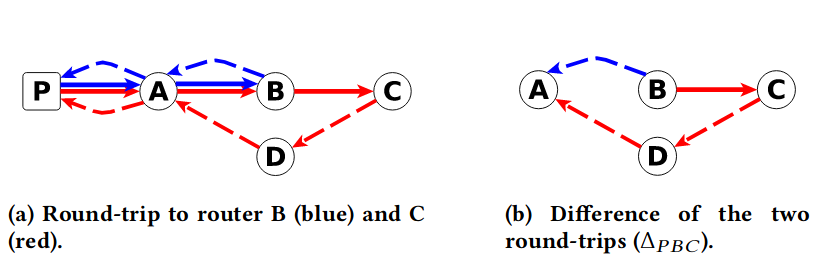
\includegraphics[width=0.7\linewidth]{illustrations/rtt-differ}
	\caption{(a) Le RTT entre la sonde P et les routeurs B et C. (b) La différence entre les  chemins de retour depuis les routeurs B et C vers la sonde P. Source : \cite{DBLP:journals/corr/FontugneAPB16}}
	\label{fig:rtt-differ}
\end{figure} 
Le RTT différentiel $ \Delta_{PBC} $ de la Figure 	\ref{fig:rtt-differ} (b) est décomposé comme suit :
\begin{align}
RTT_{PB} & =  \delta_{PA} + \delta_{AB} + \delta_{BA} + \delta_{AP} \nonumber\\
RTT_{PC} & = \delta_{PA} + \delta_{AB} + \delta_{BC} + \delta_{CD} + \delta_{DA}+ \delta_{AP} \nonumber\\
\Delta_{PBC} & = RTT_{PC} - RTT_{PB}  \label{eq:rttdifference}\\ 
& =  \delta_{BC} + \delta_{CD} + \delta_{DA}- \delta_{BA} \nonumber \\
& = \delta_{BC} + \varepsilon_{PBC} \label{eq:rttdiff}
\end{align}

où $\delta_{BC}$ est le délai du lien $BC$ et $\varepsilon_{PBC}$ est la différence entre les deux chemins de retour : $B$ vers $P$ et $C$ vers $P$.  Le chemin de retour est celui  présenté dans  la Figure \ref{fig:rtt-differ} (b). 
Nous notons qu'en pratique, un RTT différentiel peut avoir des valeurs négatives ($ \Delta_{XY} < 0 $). Car $Y$ a un RTT plus petit que celui de $ X $, cela résulte de l'asymétrie du trafic. 
Le suivi des performances du réseau avec traceroute soulève trois défis majeurs : la variété des RTTs, les pertes de paquets et l'asymétrie du trafic. Ces défis sont discutés dans le travail de référence \cite{DBLP:journals/corr/FontugneAPB16}.

%La première composante dépend de l'état des routeurs $B$ et $C$. La deuxième composante dépend de la sonde $P$. L'analyse du RTT différentiel repose sur la variation de valeurs qu'il prend, au lieu des valeurs exactes, dans  le cas des valeurs exactes, elles peuvent dévier l'interprétation.


\paragraph{Le principe de la détection des changements des délais}~

L'évolution du délai d'un lien est déduit de l'évolution de son RTT différentiel. Reprenons d'abord l'équation (\ref{eq:rttdiff}) du RTT différentiel du lien BC. Les deux variables $\delta_{BC}$ et $\varepsilon_{PBC}$ sont affectées par des facteurs différents.
La valeur de  $\delta_{BC}$ dépend de l'état des deux routeurs B et C et ne dépend pas de la sonde P. Tandis que la valeur de $\varepsilon_{PBC}$ dépend de la sonde P.

Supposons qu'on dispose d'un nombre $n$ de sondes Atlas P$_i$, $i$ $\in$ [$1$, $n$], telles que toutes les sondes ont un chemin de retour  $\varepsilon_{P_{i}BC}$ différent depuis B et depuis C.  Les $n$ RTTs différentiels $\Delta_{P{_i}BC}$ du lien $BC$ pour chacune des sondes $P_i$  partagent la même composante $\delta_{BC}$ :


\begin{align*}
\Delta_{P_{1}BC} &= \delta_{BC} + \varepsilon_{P_{1}BC}\\
\Delta_{P_{2}BC} &= \delta_{BC} + \varepsilon_{P_{2}BC}\\
.... &   ... \\
\Delta_{P_{i}BC} &= \delta_{BC} + \varepsilon_{P_{i}BC}\\
\Delta_{P_{n}BC} &= \delta_{BC} + \varepsilon_{P_{n}BC}\\
\end{align*}

Les valeurs de  $\varepsilon_{P_{i}BC}$ sont  indépendantes. L'indépendance de ces valeurs implique que la distribution $\Delta_{P_{i}BC}$ est estimé  stable au cours du temps si $\delta_{BC}$ est constant. Toutefois, un changement significatif de la valeur de $\delta_{BC}$ influence les valeurs des RTTs différentiels, ainsi,  la distribution des RTTs différentiels ($\Delta_{P_{i}BC}$) change. D'où l'idée de l'évolution du délai d'un lien déduit  à partir de l'évolution de son RTT différentiel.

\paragraph{Caractérisation des délais d'un lien}~

Les auteurs du travail de référence  ont évalué le délai d'un lien en évaluant son RTT différentiel. Cette évaluation repose sur le théorème central limite énoncé ci-dessous\footnote{Voir le théorème  $ 4.11.1 $ dans \cite{lefebvre2003cours}.}.

\begin{tcolorbox}
	Soient $X_1$, ..., $X_n$ $n$ variables aléatoires \textit{i.i.d}. de moyenne $\mu$ et de variance $\sigma^2$ finies ($\sigma > 0$). Soient $S_n$ la somme des $n$ variables aléatoires et 
	\begin{equation}
	Z_n := \frac{S_n - n\mu}{\sqrt{n} \sigma}.
	\end{equation} 
	Alors la fonction de répartition de $Z_n$ tend vers celle d'une loi $N(0,1)$ lorsque $n$ tend vers l'infini.
	
	Remarque : on peut aussi écrire le résultat suivant :
	\begin{equation}
	Sn \approx N(n\mu, n\sigma^2)
	\end{equation}
\end{tcolorbox}

L'application de ce théorème, dans  l'analyse des délais des liens, implique que quelque soit la distribution des RTTs différentiels, la moyenne arithmétique d'un échantillon  est distribuée normalement si la taille de l'échantillon est relativement grande. En pratique,
si un lien subit un changement anormal, la distribution de la moyenne des RTTs différentiels dévie de la distribution normale, par conséquent, la moyenne des RTTs différentiels ayant produit ce changement est identifiée comme  étant une anomalie.

Après avoir évalué les premiers résultats d'application de ce théorème, les auteurs ont conclu que l'utilisation de la médiane,  au lieu de la moyenne, a montré plus de performance en terme de détection des anomalies.
Afin de tenir compte de l'incertitude dans la médiane calculée, ayant la capacité d'identifier un changement anormal, les auteurs ont  calculé  l'intervalle de confiance de cette dernière.
%La distribution des médianes des RTTs différentiels caractérisant un lien est mise à jour tout au long de l'analyse des différentes périodes. 
Par définition\footnote{Definition 2.1 dans \cite{leboudec2010performance}.},  un intervalle de confiance à un niveau $\gamma$,  d'un paramètre $m$ fixé mais inconnu est l'intervalle  $(u(X_1,...,X_n),v(X_1,...,X_n)) $ tel que  :

\begin{align}
\mathbb{P}(u(X_1,...,X_n)< m< v(X_1,...,X_n)) \geq \gamma
\end{align}

\section{L'étude des délais des liens en pratique : l'évolution du RTT différentiel des liens}

L'évolution des RTTs différentiels est une  application du principe décrit dans la section  \ref{principe-de-detection}. Pour un lien donné, le suivi s'étale sur plusieurs  périodes consécutives.  

\subsection{Les étapes principales de détection} \label{steps:detection}
Les étapes du processus de détection peuvent être résumées dans les éléments suivants:

\begin{enumerate}[label=(\roman*)]
	
	\item Vérification de la validité de tout traceroute.
	
	\item Identification et calcul des RTTs différentiels de chaque lien identifié dans les traceroutes.
	
	\item Caractérisation des liens avec le théorème central limite (CLT).
	
	\item  Comparaison de l'état de chaque lien avec sa référence  et l'identification des anomalies.
	
	\item Mise à jour de la référence du lien.
\end{enumerate}

\subsection{Description des paramètres de l'analyse des délais} \label{par:parametre-de-lanalyse}~
La détection des changements des délais nécessite l'ajustement de quelques paramètres. Ces paramètres ont des valeurs par défaut  définies dans le travail de référence. Nous décrivons ci-dessous tous les paramètres : ceux ayant une valeur par défaut et ceux à ajuster :

\begin{description}
	\item[traceroutes] : ce sont l'ensemble des résultats de requêtes traceroute. La détection des anomalies est effectuée suivant le nombre de traceroutes analysés et la période précisée. 
	%Les  traceroutes sont obtenus en utilisant l'API fournie par Atlas.
	\item[start] : c'est la date de début de l'analyse. Seuls les traceroutes effectués par les sondes  à partir de cette date sont analysés.
	\item[end]  : c'est la date marquant la fin de l'analyse. Comme le paramètre \textit{start}, c'est la date maximale des  traceroutes à considérer effectués par les sondes.
	\item[timeWindow]:  ce paramètre est exprimé en secondes. Il correspond à la durée de chaque période des $n$ périodes de l'analyse. Ces périodes ont la même durée. Autrement dit, la durée entre   \textit{start} et \textit{end} est divisée par \textit{timeWindow}. Ceci est illustré à la Figure  \ref{fig:timing_tex_}. Avec $d_i$ dénote le début de la i\up{ème} période,  $i \in [1,n]$. Par défaut, \textit{timeWindow} vaut $ 3600 $ secondes. 
	%illustre le contexte des trois paramètres \textit{start}, \textit{end} et \textit{timeWindow} avec les étapes principales
	\begin{figure}[h]
		\centering
		\captionsetup{justification=centering}
		% Graphic for TeX using PGF
% Title: /home/hayat/RipeAtlasTraceroutesAnalysis/report/illustrations/timing.dia
% Creator: Dia v0.97+git
% CreationDate: Mon Dec  3 23:19:01 2018
% For: hayat
% \usepackage{tikz}
% The following commands are not supported in PSTricks at present
% We define them conditionally, so when they are implemented,
% this pgf file will use them.
\ifx\du\undefined
  \newlength{\du}
\fi
\setlength{\du}{15\unitlength}
\begin{tikzpicture}[even odd rule]
\pgftransformxscale{1.000000}
\pgftransformyscale{-1.000000}
\definecolor{dialinecolor}{rgb}{0.000000, 0.000000, 0.000000}
\pgfsetstrokecolor{dialinecolor}
\pgfsetstrokeopacity{1.000000}
\definecolor{diafillcolor}{rgb}{1.000000, 1.000000, 1.000000}
\pgfsetfillcolor{diafillcolor}
\pgfsetfillopacity{1.000000}
\pgfsetlinewidth{0.100000\du}
\pgfsetdash{}{0pt}
\pgfsetbuttcap
{
\definecolor{diafillcolor}{rgb}{0.000000, 0.000000, 0.000000}
\pgfsetfillcolor{diafillcolor}
\pgfsetfillopacity{1.000000}
% was here!!!
}
\definecolor{dialinecolor}{rgb}{0.000000, 0.000000, 0.000000}
\pgfsetstrokecolor{dialinecolor}
\pgfsetstrokeopacity{1.000000}
\draw (34.600000\du,6.050000\du)--(40.550000\du,6.000000\du);
\pgfsetlinewidth{0.100000\du}
\pgfsetdash{}{0pt}
\pgfsetmiterjoin
\pgfsetbuttcap
\definecolor{dialinecolor}{rgb}{0.000000, 0.000000, 0.000000}
\pgfsetstrokecolor{dialinecolor}
\pgfsetstrokeopacity{1.000000}
\draw (35.097882\du,5.795807\du)--(35.102083\du,6.295790\du);
\pgfsetlinewidth{0.100000\du}
\pgfsetdash{}{0pt}
\pgfsetmiterjoin
\pgfsetbuttcap
\definecolor{dialinecolor}{rgb}{0.000000, 0.000000, 0.000000}
\pgfsetstrokecolor{dialinecolor}
\pgfsetstrokeopacity{1.000000}
\draw (40.052118\du,6.254193\du)--(40.047917\du,5.754210\du);
% setfont left to latex
\definecolor{dialinecolor}{rgb}{0.000000, 0.000000, 0.000000}
\pgfsetstrokecolor{dialinecolor}
\pgfsetstrokeopacity{1.000000}
\definecolor{diafillcolor}{rgb}{0.000000, 0.000000, 0.000000}
\pgfsetfillcolor{diafillcolor}
\pgfsetfillopacity{1.000000}
\node[anchor=base west,inner sep=0pt,outer sep=0pt,color=dialinecolor] at (14.800200\du,8.464650\du){start};
% setfont left to latex
\definecolor{dialinecolor}{rgb}{0.000000, 0.000000, 0.000000}
\pgfsetstrokecolor{dialinecolor}
\pgfsetstrokeopacity{1.000000}
\definecolor{diafillcolor}{rgb}{0.000000, 0.000000, 0.000000}
\pgfsetfillcolor{diafillcolor}
\pgfsetfillopacity{1.000000}
\node[anchor=base west,inner sep=0pt,outer sep=0pt,color=dialinecolor] at (39.375600\du,7.990890\du){end};
% setfont left to latex
\definecolor{dialinecolor}{rgb}{0.000000, 0.000000, 0.000000}
\pgfsetstrokecolor{dialinecolor}
\pgfsetstrokeopacity{1.000000}
\definecolor{diafillcolor}{rgb}{0.000000, 0.000000, 0.000000}
\pgfsetfillcolor{diafillcolor}
\pgfsetfillopacity{1.000000}
\node[anchor=base west,inner sep=0pt,outer sep=0pt,color=dialinecolor] at (24.374800\du,8.977310\du){Périodes de l'analyse};
% setfont left to latex
\definecolor{dialinecolor}{rgb}{0.000000, 0.000000, 0.000000}
\pgfsetstrokecolor{dialinecolor}
\pgfsetstrokeopacity{1.000000}
\definecolor{diafillcolor}{rgb}{0.000000, 0.000000, 0.000000}
\pgfsetfillcolor{diafillcolor}
\pgfsetfillopacity{1.000000}
\node[anchor=base west,inner sep=0pt,outer sep=0pt,color=dialinecolor] at (14.950000\du,7.200000\du){d1};
\pgfsetlinewidth{0.100000\du}
\pgfsetdash{}{0pt}
\pgfsetbuttcap
{
\definecolor{diafillcolor}{rgb}{0.000000, 0.000000, 0.000000}
\pgfsetfillcolor{diafillcolor}
\pgfsetfillopacity{1.000000}
% was here!!!
}
\definecolor{dialinecolor}{rgb}{0.000000, 0.000000, 0.000000}
\pgfsetstrokecolor{dialinecolor}
\pgfsetstrokeopacity{1.000000}
\draw (29.656800\du,6.066270\du)--(35.606800\du,6.016270\du);
\pgfsetlinewidth{0.100000\du}
\pgfsetdash{}{0pt}
\pgfsetmiterjoin
\pgfsetbuttcap
\definecolor{dialinecolor}{rgb}{0.000000, 0.000000, 0.000000}
\pgfsetstrokecolor{dialinecolor}
\pgfsetstrokeopacity{1.000000}
\draw (30.154682\du,5.812077\du)--(30.158883\du,6.312060\du);
\pgfsetlinewidth{0.100000\du}
\pgfsetdash{}{0pt}
\pgfsetmiterjoin
\pgfsetbuttcap
\definecolor{dialinecolor}{rgb}{0.000000, 0.000000, 0.000000}
\pgfsetstrokecolor{dialinecolor}
\pgfsetstrokeopacity{1.000000}
\draw (35.108918\du,6.270463\du)--(35.104717\du,5.770480\du);
\pgfsetlinewidth{0.100000\du}
\pgfsetdash{}{0pt}
\pgfsetbuttcap
{
\definecolor{diafillcolor}{rgb}{0.000000, 0.000000, 0.000000}
\pgfsetfillcolor{diafillcolor}
\pgfsetfillopacity{1.000000}
% was here!!!
}
\definecolor{dialinecolor}{rgb}{0.000000, 0.000000, 0.000000}
\pgfsetstrokecolor{dialinecolor}
\pgfsetstrokeopacity{1.000000}
\draw (24.701800\du,6.106100\du)--(30.651800\du,6.056100\du);
\pgfsetlinewidth{0.100000\du}
\pgfsetdash{}{0pt}
\pgfsetmiterjoin
\pgfsetbuttcap
\definecolor{dialinecolor}{rgb}{0.000000, 0.000000, 0.000000}
\pgfsetstrokecolor{dialinecolor}
\pgfsetstrokeopacity{1.000000}
\draw (25.199682\du,5.851907\du)--(25.203883\du,6.351890\du);
\pgfsetlinewidth{0.100000\du}
\pgfsetdash{}{0pt}
\pgfsetmiterjoin
\pgfsetbuttcap
\definecolor{dialinecolor}{rgb}{0.000000, 0.000000, 0.000000}
\pgfsetstrokecolor{dialinecolor}
\pgfsetstrokeopacity{1.000000}
\draw (30.153918\du,6.310293\du)--(30.149717\du,5.810310\du);
\pgfsetlinewidth{0.100000\du}
\pgfsetdash{}{0pt}
\pgfsetbuttcap
{
\definecolor{diafillcolor}{rgb}{0.000000, 0.000000, 0.000000}
\pgfsetfillcolor{diafillcolor}
\pgfsetfillopacity{1.000000}
% was here!!!
}
\definecolor{dialinecolor}{rgb}{0.000000, 0.000000, 0.000000}
\pgfsetstrokecolor{dialinecolor}
\pgfsetstrokeopacity{1.000000}
\draw (19.796600\du,6.121020\du)--(25.746600\du,6.071020\du);
\pgfsetlinewidth{0.100000\du}
\pgfsetdash{}{0pt}
\pgfsetmiterjoin
\pgfsetbuttcap
\definecolor{dialinecolor}{rgb}{0.000000, 0.000000, 0.000000}
\pgfsetstrokecolor{dialinecolor}
\pgfsetstrokeopacity{1.000000}
\draw (20.294482\du,5.866827\du)--(20.298683\du,6.366810\du);
\pgfsetlinewidth{0.100000\du}
\pgfsetdash{}{0pt}
\pgfsetmiterjoin
\pgfsetbuttcap
\definecolor{dialinecolor}{rgb}{0.000000, 0.000000, 0.000000}
\pgfsetstrokecolor{dialinecolor}
\pgfsetstrokeopacity{1.000000}
\draw (25.248718\du,6.325213\du)--(25.244517\du,5.825230\du);
\pgfsetlinewidth{0.100000\du}
\pgfsetdash{}{0pt}
\pgfsetbuttcap
{
\definecolor{diafillcolor}{rgb}{0.000000, 0.000000, 0.000000}
\pgfsetfillcolor{diafillcolor}
\pgfsetfillopacity{1.000000}
% was here!!!
}
\definecolor{dialinecolor}{rgb}{0.000000, 0.000000, 0.000000}
\pgfsetstrokecolor{dialinecolor}
\pgfsetstrokeopacity{1.000000}
\draw (14.841600\du,6.135940\du)--(20.791600\du,6.085940\du);
\pgfsetlinewidth{0.100000\du}
\pgfsetdash{}{0pt}
\pgfsetmiterjoin
\pgfsetbuttcap
\definecolor{dialinecolor}{rgb}{0.000000, 0.000000, 0.000000}
\pgfsetstrokecolor{dialinecolor}
\pgfsetstrokeopacity{1.000000}
\draw (15.339482\du,5.881747\du)--(15.343683\du,6.381730\du);
\pgfsetlinewidth{0.100000\du}
\pgfsetdash{}{0pt}
\pgfsetmiterjoin
\pgfsetbuttcap
\definecolor{dialinecolor}{rgb}{0.000000, 0.000000, 0.000000}
\pgfsetstrokecolor{dialinecolor}
\pgfsetstrokeopacity{1.000000}
\draw (20.293718\du,6.340133\du)--(20.289517\du,5.840150\du);
% setfont left to latex
\definecolor{dialinecolor}{rgb}{0.000000, 0.000000, 0.000000}
\pgfsetstrokecolor{dialinecolor}
\pgfsetstrokeopacity{1.000000}
\definecolor{diafillcolor}{rgb}{0.000000, 0.000000, 0.000000}
\pgfsetfillcolor{diafillcolor}
\pgfsetfillopacity{1.000000}
\node[anchor=base west,inner sep=0pt,outer sep=0pt,color=dialinecolor] at (19.845000\du,7.235000\du){d2};
% setfont left to latex
\definecolor{dialinecolor}{rgb}{0.000000, 0.000000, 0.000000}
\pgfsetstrokecolor{dialinecolor}
\pgfsetstrokeopacity{1.000000}
\definecolor{diafillcolor}{rgb}{0.000000, 0.000000, 0.000000}
\pgfsetfillcolor{diafillcolor}
\pgfsetfillopacity{1.000000}
\node[anchor=base west,inner sep=0pt,outer sep=0pt,color=dialinecolor] at (24.750000\du,7.300000\du){d3};
% setfont left to latex
\definecolor{dialinecolor}{rgb}{0.000000, 0.000000, 0.000000}
\pgfsetstrokecolor{dialinecolor}
\pgfsetstrokeopacity{1.000000}
\definecolor{diafillcolor}{rgb}{0.000000, 0.000000, 0.000000}
\pgfsetfillcolor{diafillcolor}
\pgfsetfillopacity{1.000000}
\node[anchor=base west,inner sep=0pt,outer sep=0pt,color=dialinecolor] at (29.740000\du,7.175000\du){di};
% setfont left to latex
\definecolor{dialinecolor}{rgb}{0.000000, 0.000000, 0.000000}
\pgfsetstrokecolor{dialinecolor}
\pgfsetstrokeopacity{1.000000}
\definecolor{diafillcolor}{rgb}{0.000000, 0.000000, 0.000000}
\pgfsetfillcolor{diafillcolor}
\pgfsetfillopacity{1.000000}
\node[anchor=base west,inner sep=0pt,outer sep=0pt,color=dialinecolor] at (34.685000\du,7.165000\du){di+1};
\pgfsetlinewidth{0.100000\du}
\pgfsetdash{}{0pt}
\pgfsetbuttcap
\definecolor{dialinecolor}{rgb}{0.000000, 0.000000, 0.000000}
\pgfsetstrokecolor{dialinecolor}
\pgfsetstrokeopacity{1.000000}
\pgfpathmoveto{\pgfpoint{25.180033\du}{4.900033\du}}
\pgfpatharc{315}{226}{3.501250\du and 3.501250\du}
\pgfusepath{stroke}
% setfont left to latex
\definecolor{dialinecolor}{rgb}{0.000000, 0.000000, 0.000000}
\pgfsetstrokecolor{dialinecolor}
\pgfsetstrokeopacity{1.000000}
\definecolor{diafillcolor}{rgb}{0.000000, 0.000000, 0.000000}
\pgfsetfillcolor{diafillcolor}
\pgfsetfillopacity{1.000000}
\node[anchor=base west,inner sep=0pt,outer sep=0pt,color=dialinecolor] at (20.780000\du,3.400000\du){timeWindow};
\pgfsetlinewidth{0.100000\du}
\pgfsetdash{}{0pt}
\pgfsetbuttcap
\definecolor{dialinecolor}{rgb}{0.000000, 0.000000, 0.000000}
\pgfsetstrokecolor{dialinecolor}
\pgfsetstrokeopacity{1.000000}
\pgfpathmoveto{\pgfpoint{29.975033\du}{4.885033\du}}
\pgfpatharc{315}{226}{3.501250\du and 3.501250\du}
\pgfusepath{stroke}
% setfont left to latex
\definecolor{dialinecolor}{rgb}{0.000000, 0.000000, 0.000000}
\pgfsetstrokecolor{dialinecolor}
\pgfsetstrokeopacity{1.000000}
\definecolor{diafillcolor}{rgb}{0.000000, 0.000000, 0.000000}
\pgfsetfillcolor{diafillcolor}
\pgfsetfillopacity{1.000000}
\node[anchor=base west,inner sep=0pt,outer sep=0pt,color=dialinecolor] at (25.675000\du,3.485000\du){timeWindow};
\pgfsetlinewidth{0.100000\du}
\pgfsetdash{}{0pt}
\pgfsetbuttcap
\definecolor{dialinecolor}{rgb}{0.000000, 0.000000, 0.000000}
\pgfsetstrokecolor{dialinecolor}
\pgfsetstrokeopacity{1.000000}
\pgfpathmoveto{\pgfpoint{20.275033\du}{4.785033\du}}
\pgfpatharc{315}{226}{3.501250\du and 3.501250\du}
\pgfusepath{stroke}
% setfont left to latex
\definecolor{dialinecolor}{rgb}{0.000000, 0.000000, 0.000000}
\pgfsetstrokecolor{dialinecolor}
\pgfsetstrokeopacity{1.000000}
\definecolor{diafillcolor}{rgb}{0.000000, 0.000000, 0.000000}
\pgfsetfillcolor{diafillcolor}
\pgfsetfillopacity{1.000000}
\node[anchor=base west,inner sep=0pt,outer sep=0pt,color=dialinecolor] at (16.025000\du,3.435000\du){timeWindow};
\end{tikzpicture}

		\caption{Illustration des périodes de l'analyse entre la date de début et la date de fin.}
		\label{fig:timing_tex_}
	\end{figure}
	%\begin{figure}[h]	
	%	\centering
	%	\resizebox{\textwidth}{!}{
	%		% Graphic for TeX using PGF
% Title: /home/bellafkih/Documents/2018-2019/memoire/rapport_memoire/dia/timewindow.dia
% Creator: Dia v0.97.3
% CreationDate: Sun Oct  7 15:34:20 2018
% For: bellafkih
% \usepackage{tikz}
% The following commands are not supported in PSTricks at present
% We define them conditionally, so when they are implemented,
% this pgf file will use them.
\ifx\du\undefined
  \newlength{\du}
\fi
\setlength{\du}{15\unitlength}
\begin{tikzpicture}
\pgftransformxscale{1.000000}
\pgftransformyscale{-1.000000}
\definecolor{dialinecolor}{rgb}{0.000000, 0.000000, 0.000000}
\pgfsetstrokecolor{dialinecolor}
\definecolor{dialinecolor}{rgb}{1.000000, 1.000000, 1.000000}
\pgfsetfillcolor{dialinecolor}
\pgfsetlinewidth{0.200000\du}
\pgfsetdash{}{0pt}
\pgfsetdash{}{0pt}
\pgfsetbuttcap
{
\definecolor{dialinecolor}{rgb}{0.000000, 0.000000, 0.000000}
\pgfsetfillcolor{dialinecolor}
% was here!!!
\pgfsetarrowsend{to}
\definecolor{dialinecolor}{rgb}{0.000000, 0.000000, 0.000000}
\pgfsetstrokecolor{dialinecolor}
\draw (10.000000\du,2.000000\du)--(10.000000\du,26.650000\du);
}
% setfont left to latex
\definecolor{dialinecolor}{rgb}{0.000000, 0.000000, 0.000000}
\pgfsetstrokecolor{dialinecolor}
\node[anchor=west] at (7.650000\du,2.050000\du){start};
% setfont left to latex
\definecolor{dialinecolor}{rgb}{0.000000, 0.000000, 0.000000}
\pgfsetstrokecolor{dialinecolor}
\node[anchor=west] at (7.850000\du,22.100000\du){end};
\pgfsetlinewidth{0.000000\du}
\pgfsetdash{}{0pt}
\pgfsetdash{}{0pt}
\pgfsetbuttcap
{
\definecolor{dialinecolor}{rgb}{0.000000, 0.000000, 0.000000}
\pgfsetfillcolor{dialinecolor}
% was here!!!
\definecolor{dialinecolor}{rgb}{0.000000, 0.000000, 0.000000}
\pgfsetstrokecolor{dialinecolor}
\draw (10.600000\du,2.000000\du)--(9.450000\du,2.000000\du);
}
\pgfsetlinewidth{0.000000\du}
\pgfsetdash{}{0pt}
\pgfsetdash{}{0pt}
\pgfsetbuttcap
{
\definecolor{dialinecolor}{rgb}{0.000000, 0.000000, 0.000000}
\pgfsetfillcolor{dialinecolor}
% was here!!!
\definecolor{dialinecolor}{rgb}{0.000000, 0.000000, 0.000000}
\pgfsetstrokecolor{dialinecolor}
\draw (10.585000\du,5.960000\du)--(9.435000\du,5.960000\du);
}
\pgfsetlinewidth{0.000000\du}
\pgfsetdash{}{0pt}
\pgfsetdash{}{0pt}
\pgfsetbuttcap
{
\definecolor{dialinecolor}{rgb}{0.000000, 0.000000, 0.000000}
\pgfsetfillcolor{dialinecolor}
% was here!!!
\definecolor{dialinecolor}{rgb}{0.000000, 0.000000, 0.000000}
\pgfsetstrokecolor{dialinecolor}
\draw (10.570000\du,10.020000\du)--(9.420000\du,10.020000\du);
}
\pgfsetlinewidth{0.000000\du}
\pgfsetdash{}{0pt}
\pgfsetdash{}{0pt}
\pgfsetbuttcap
{
\definecolor{dialinecolor}{rgb}{0.000000, 0.000000, 0.000000}
\pgfsetfillcolor{dialinecolor}
% was here!!!
\definecolor{dialinecolor}{rgb}{0.000000, 0.000000, 0.000000}
\pgfsetstrokecolor{dialinecolor}
\draw (10.505000\du,13.930000\du)--(9.355000\du,13.930000\du);
}
\pgfsetlinewidth{0.000000\du}
\pgfsetdash{}{0pt}
\pgfsetdash{}{0pt}
\pgfsetbuttcap
{
\definecolor{dialinecolor}{rgb}{0.000000, 0.000000, 0.000000}
\pgfsetfillcolor{dialinecolor}
% was here!!!
\definecolor{dialinecolor}{rgb}{0.000000, 0.000000, 0.000000}
\pgfsetstrokecolor{dialinecolor}
\draw (10.540000\du,17.940000\du)--(9.390000\du,17.940000\du);
}
\pgfsetlinewidth{0.000000\du}
\pgfsetdash{}{0pt}
\pgfsetdash{}{0pt}
\pgfsetbuttcap
{
\definecolor{dialinecolor}{rgb}{0.000000, 0.000000, 0.000000}
\pgfsetfillcolor{dialinecolor}
% was here!!!
\definecolor{dialinecolor}{rgb}{0.000000, 0.000000, 0.000000}
\pgfsetstrokecolor{dialinecolor}
\draw (10.575000\du,22.050000\du)--(9.425000\du,22.050000\du);
}
\pgfsetlinewidth{0.000000\du}
\pgfsetdash{}{0pt}
\pgfsetdash{}{0pt}
\pgfsetbuttcap
{
\definecolor{dialinecolor}{rgb}{0.000000, 0.000000, 0.000000}
\pgfsetfillcolor{dialinecolor}
% was here!!!
\pgfsetarrowsstart{to}
\pgfsetarrowsend{to}
\definecolor{dialinecolor}{rgb}{0.000000, 0.000000, 0.000000}
\pgfsetstrokecolor{dialinecolor}
\pgfpathmoveto{\pgfpoint{6.950071\du}{2.049940\du}}
\pgfpatharc{231}{129}{2.448949\du and 2.448949\du}
\pgfusepath{stroke}
}
% setfont left to latex
\definecolor{dialinecolor}{rgb}{0.000000, 0.000000, 0.000000}
\pgfsetstrokecolor{dialinecolor}
\node[anchor=west] at (2.150000\du,26.900000\du){Temps en secondes (s)};
\pgfsetlinewidth{0.000000\du}
\pgfsetdash{}{0pt}
\pgfsetdash{}{0pt}
\pgfsetbuttcap
{
\definecolor{dialinecolor}{rgb}{0.000000, 0.000000, 0.000000}
\pgfsetfillcolor{dialinecolor}
% was here!!!
\pgfsetarrowsstart{to}
\pgfsetarrowsend{to}
\definecolor{dialinecolor}{rgb}{0.000000, 0.000000, 0.000000}
\pgfsetstrokecolor{dialinecolor}
\pgfpathmoveto{\pgfpoint{7.049251\du}{6.119940\du}}
\pgfpatharc{231}{129}{2.448949\du and 2.448949\du}
\pgfusepath{stroke}
}
\pgfsetlinewidth{0.000000\du}
\pgfsetdash{}{0pt}
\pgfsetdash{}{0pt}
\pgfsetbuttcap
{
\definecolor{dialinecolor}{rgb}{0.000000, 0.000000, 0.000000}
\pgfsetfillcolor{dialinecolor}
% was here!!!
\pgfsetarrowsstart{to}
\pgfsetarrowsend{to}
\definecolor{dialinecolor}{rgb}{0.000000, 0.000000, 0.000000}
\pgfsetstrokecolor{dialinecolor}
\pgfpathmoveto{\pgfpoint{6.984251\du}{10.079940\du}}
\pgfpatharc{231}{129}{2.448949\du and 2.448949\du}
\pgfusepath{stroke}
}
\pgfsetlinewidth{0.000000\du}
\pgfsetdash{}{0pt}
\pgfsetdash{}{0pt}
\pgfsetbuttcap
{
\definecolor{dialinecolor}{rgb}{0.000000, 0.000000, 0.000000}
\pgfsetfillcolor{dialinecolor}
% was here!!!
\pgfsetarrowsstart{to}
\pgfsetarrowsend{to}
\definecolor{dialinecolor}{rgb}{0.000000, 0.000000, 0.000000}
\pgfsetstrokecolor{dialinecolor}
\pgfpathmoveto{\pgfpoint{6.869251\du}{14.089940\du}}
\pgfpatharc{231}{129}{2.448949\du and 2.448949\du}
\pgfusepath{stroke}
}
\pgfsetlinewidth{0.000000\du}
\pgfsetdash{}{0pt}
\pgfsetdash{}{0pt}
\pgfsetbuttcap
{
\definecolor{dialinecolor}{rgb}{0.000000, 0.000000, 0.000000}
\pgfsetfillcolor{dialinecolor}
% was here!!!
\pgfsetarrowsstart{to}
\pgfsetarrowsend{to}
\definecolor{dialinecolor}{rgb}{0.000000, 0.000000, 0.000000}
\pgfsetstrokecolor{dialinecolor}
\pgfpathmoveto{\pgfpoint{6.954251\du}{18.099940\du}}
\pgfpatharc{231}{129}{2.448949\du and 2.448949\du}
\pgfusepath{stroke}
}
% setfont left to latex
\definecolor{dialinecolor}{rgb}{0.000000, 0.000000, 0.000000}
\pgfsetstrokecolor{dialinecolor}
\node[anchor=west] at (0.650000\du,4.050000\du){timeWindow s};
% setfont left to latex
\definecolor{dialinecolor}{rgb}{0.000000, 0.000000, 0.000000}
\pgfsetstrokecolor{dialinecolor}
\node[anchor=west] at (0.685100\du,8.005000\du){timeWindow s};
% setfont left to latex
\definecolor{dialinecolor}{rgb}{0.000000, 0.000000, 0.000000}
\pgfsetstrokecolor{dialinecolor}
\node[anchor=west] at (0.870100\du,12.015000\du){timeWindow s};
% setfont left to latex
\definecolor{dialinecolor}{rgb}{0.000000, 0.000000, 0.000000}
\pgfsetstrokecolor{dialinecolor}
\node[anchor=west] at (0.905100\du,16.025000\du){timeWindow s};
% setfont left to latex
\definecolor{dialinecolor}{rgb}{0.000000, 0.000000, 0.000000}
\pgfsetstrokecolor{dialinecolor}
\node[anchor=west] at (1.040100\du,19.935000\du){timeWindow s};
% setfont left to latex
\definecolor{dialinecolor}{rgb}{0.000000, 0.000000, 0.000000}
\pgfsetstrokecolor{dialinecolor}
\node[anchor=west] at (11.200100\du,3.850000\du){appliquer : computeRtt(), mergeRttResults(), outlierDetection()};
% setfont left to latex
\definecolor{dialinecolor}{rgb}{0.000000, 0.000000, 0.000000}
\pgfsetstrokecolor{dialinecolor}
\node[anchor=west] at (11.035100\du,7.905000\du){appliquer : computeRtt(), mergeRttResults(), outlierDetection()};
% setfont left to latex
\definecolor{dialinecolor}{rgb}{0.000000, 0.000000, 0.000000}
\pgfsetstrokecolor{dialinecolor}
\node[anchor=west] at (11.120100\du,12.015000\du){appliquer : computeRtt(), mergeRttResults(), outlierDetection()};
% setfont left to latex
\definecolor{dialinecolor}{rgb}{0.000000, 0.000000, 0.000000}
\pgfsetstrokecolor{dialinecolor}
\node[anchor=west] at (11.105100\du,15.875000\du){appliquer : computeRtt(), mergeRttResults(), outlierDetection()};
% setfont left to latex
\definecolor{dialinecolor}{rgb}{0.000000, 0.000000, 0.000000}
\pgfsetstrokecolor{dialinecolor}
\node[anchor=west] at (11.040100\du,19.885000\du){appliquer : computeRtt(), mergeRttResults(), outlierDetection()};
% setfont left to latex
\definecolor{dialinecolor}{rgb}{0.000000, 0.000000, 0.000000}
\pgfsetstrokecolor{dialinecolor}
\node[anchor=west] at (11.950100\du,2.000000\du){inputs : paramère de l'expérience};
% setfont left to latex
\definecolor{dialinecolor}{rgb}{0.000000, 0.000000, 0.000000}
\pgfsetstrokecolor{dialinecolor}
\node[anchor=west] at (12.050100\du,22.000000\du){output : les changements détéctés et ses caractériqtiques};
\end{tikzpicture}
 
	%	}
	%	\caption{Illustration du paramètre timeWindow}
	%	\label{fig:timewindow}
	%\end{figure}
	\item[minSeen] : est le nombre de fenêtres à atteindre avant de commencer la comparaison du RTT différentiel d'un lien avec sa référence. 
	%comme l'analyse des liens est réalisée sur plusieurs périodes de durée \textit{timeWindow}, 
	%ce paramètre est un entier, il indique le déclenchement de la comparaison du RTT différentiel de référence d'un lien avec sa valeur courante.  
	%Par exemple, si $ minSeen = 24 $ et $timeWindow = 3600$ (1 heure), cela implique que la première référence de tout lien est construite des valeurs obtenues tout au long la durée $24 * timeWindow$, donc après avoir analysé les traceroutes d'une journée. A la 25\up{ème} \textit{timeWindow}, la détection des anomalies s'effectue.
	% nombre de fois à partir desquelles on peut  vérifier son RTT différentiel; s'il indique une anomalie ou non. 
	%Par exemple, un lien peut être identifié dans $3$ $d_i$, ou bien être identifié  une seule fois durant toute la période de l'analyse.
	
	\item[alpha ]: noté $\alpha$,  $\alpha \in [0, 1]$, c'est le paramètre de la  moyenne mobile exponentielle calculée.
	%\guillemotleft \textit{ Les méthodes de lissage exponentiel  sont un ensemble de techniques empiriques de prévision qui accordent plus ou moins d'importance aux valeurs du passé d'une série temporelle\footnote{Source : \url{https://perso.math.univ-toulouse.fr/lagnoux/files/2013/12/Chap6.pdf}, consultée le $30/09/2018.$}}. \guillemotright
	
	La  moyenne mobile exponentielle est utilisée pour calculer la moyenne des RTTs différentiels de référence durant une période $d_k$.
	% Cette médiane constitue une référence  sur laquelle se base la détection des anomalies.
	La  valeur de la médiane des RTTs différentiels de référence $ \overline{m}_{t}$   pour la période $ t $ et  le lien $l$ est:
	\begin{align*}
	\overline{m}_{t} &=  \alpha{m}_{t} + (1 -  \alpha)  \overline{m}_{t-1}
	\end{align*} 
	$m_t$ la médiane des RTTs différentiels observée pour $l$ durant la \textit{période} $t$. 
	
	$ \overline{m}_{t-1}$  la médiane des  RTTs différentiels  de référence durant la \textit{période} $ t-1 $.  
	
	
	
	Pour précision, \{$m_t$\} et \{$ \overline{m}_{t}$\} désignent deux ensembles différents.   Le premier est l'ensemble des médianes des RTTs différentiels de chaque période $d_k$. Or, le deuxième est l'ensemble des médianes des RTTs différentiels, de référence, construite en utilisant la méthode de la moyenne mobile exponentielle. Le calcul de cette dernière prend en compte les médianes des RTTs différentiels précédentes ainsi que la médiane des RTTs différentiels courante. La participation de ces dernières dans le calcul de la référence est dirigé par le paramètre $\alpha$. Plus de détails sur ce calcul est donné dans la section  \ref{reference-lissage}.
	%La  valeur de la médiane de référence  $ \overline{m}_{t}$ de la période $t$ est obtenue par: 
	
	
	
	Le paramètre $\alpha$  contrôle l'importance  des mesures précédentes par rapport aux mesures récentes. De ce fait, \guillemotleft \textit{plus $\alpha$ est proche de $ 1 $ plus les observations récentes influent sur la prévision, à l'inverse un $\alpha$ proche de $0$ conduit à une prévision très stable prenant en compte un passé lointain}\footnote{Voir le lissage exponentiel dans \url{https://www.math.u-psud.fr/~goude/Materials/time_series/cours3_lissage_expo.pdf}, consultée le $30/09/2018$.}.\guillemotright.  Dans le travail de référence, le paramètre $\alpha$  vaut par défaut $0.01$.
	
	
	\item[confInterval] : ce paramètre indique le niveau de confiance de l'intervalle de confiance de la médiane calculée des RTTs différentiels. Précisément, cet intervalle de confiance calculé est de niveau de confiance égal à $ 1 - confInterval $.  L'intervalle de confiance d'une moyenne  est défini comme représentant les valeurs probables que peut prendre cette moyenne, si on accepte une marge d'erreur définie à l'avance. Avec la variante adoptée, on parle de la médiane des RTTs différentiels. Il existe plusieurs méthodes pour calculer l'intervalle de confiance d'une proportion. Parmi les critères impliqués sur le choix de la méthode du calcul, on note le nombre total d'expériences.
	
	Au RTT différentiel courant et  au celui de référence d'un lien donné sont associés des intervalles de confiance.  Le calcul des intervalles de confiance  est approché par le score de Wilson. Le score de wilson a été adopté car il donne des résultats même si la distribution pour laquelle l'intervalle de confiance est calculé est petite. Pour chaque lien et pour chaque période $d_k$,  deux intervalles de confiances sont calculés, pour ensuite évaluer le chevauchement entre ces deux intervalles. L'outil de détection utilise une marge d'erreur égale à  $ 0.05 $. Les détails du calcul des intervalles de confiances sont fournis dans la section \ref{conf-inter-section-exemple}.
\end{description}


\subsection{Processus de  détection des anomalies  : notation formelle}\label{steps-rtt-analysis}

Soient $ d_1 $, $  d_2 $, $d_k$, ..., $ d_n $ l'ensemble $D$ de $n$ périodes entre \textit{start} et \textit{end} avec $k \in [1,n]$. La différence entre le début de la période $ d_{k+1} $ et le début de la période $ d_k $ est égale à $timeWindow$ pour tout $k+1 \leq n $.  

Le processus de la détection des anomalies, selon l'implémentation \cite{InternetHealthReport} des auteurs du travail de référence,  passe par plusieurs étapes. D'abord on  regroupe les traceroutes à analyser par période $d_k$ (étape $ 1 $). Ensuite, on prépare les traceroutes de toute  période $d_k$ en y appliquant un nombre d'opérations (étapes  $ 2 $ à $ 6 $) afin d'énumérer les liens possibles avec leurs RTTs différentiels. A la fin de la préparation des traceroutes de toutes les périodes, nous obtenons une liste de liens par période. Nous résumons ensuite ces liens en fusionnant les mêmes liens identifiés durant toutes les périodes tout en conservant la période pendant laquelle il a été identifié. Sur base des détails d'un lien donné,  nous identifions les anomalies dans leurs délais (étapes $ 7 $ à $9$). 

\subparagraph{Notations} Chaque traceroute contient un ensemble de sauts, et chaque saut contient un ensemble de signaux. Chaque signal se caractérise par le routeur émettant ce signal et le RTT correspondant. 
Soit  $h_i$ le i\up{ème} saut d'un traceroute donné tel que

 $h_i =\{s_{i,j} |  j \in [1, S], i\in [1,H]  \}$, $S$ et $H$ sont des entiers. Soit $ s_{i,j} $  le j\up{ème} signal du i\up{ème} saut, il se caractérise par le routeur  source du signal $from_{i,j}$ et le RTT correspondant est $rtt_{i,j}$.

Un traceroute  est un ensemble de sauts $h_i$ auxquels sont joints l'identifiant de la sonde ayant effectué la requête traceroute  la destination de la requête, le temps de la requête, etc. Chaque saut est décrit par un ensemble de signaux dans  $S$.  Chaque signal décrit le routeur ayant émis une réponse à la sonde parmi les routeurs traversés avant d'atteindre la destination finale.  Pour le saut $h_i$, on note trois\footnote{Le nombre trois peut varier dans certains cas. L'outil de détection conçu est adapté à tout nombre de signaux.} signaux $s_{i, j},  j\in [1,3]$ dont le routeur émettant le signal est $from_{i,j}$ et son RTT est égal à $rtt_{i,j}$. C'est ce qu'illustre  la Figure \ref{fig:traceroute}.

\begin{figure}[H]
	\centering
	\captionsetup{justification=centering}
	\resizebox{\textwidth}{!}{
		% Graphic for TeX using PGF
% Title: /home/hayat/RipeAtlasTraceroutesAnalysis/report/illustrations/dia/traceroute_.dia
% Creator: Dia v0.97+git
% CreationDate: Fri Dec 28 18:14:49 2018
% For: hayat
% \usepackage{tikz}
% The following commands are not supported in PSTricks at present
% We define them conditionally, so when they are implemented,
% this pgf file will use them.
\ifx\du\undefined
  \newlength{\du}
\fi
\setlength{\du}{15\unitlength}
\begin{tikzpicture}[even odd rule]
\pgftransformxscale{1.000000}
\pgftransformyscale{-1.000000}
\definecolor{dialinecolor}{rgb}{0.000000, 0.000000, 0.000000}
\pgfsetstrokecolor{dialinecolor}
\pgfsetstrokeopacity{1.000000}
\definecolor{diafillcolor}{rgb}{1.000000, 1.000000, 1.000000}
\pgfsetfillcolor{diafillcolor}
\pgfsetfillopacity{1.000000}
\pgfsetlinewidth{0.100000\du}
\pgfsetdash{}{0pt}
\pgfsetmiterjoin
{\pgfsetcornersarced{\pgfpoint{0.000000\du}{0.000000\du}}\definecolor{diafillcolor}{rgb}{1.000000, 1.000000, 1.000000}
\pgfsetfillcolor{diafillcolor}
\pgfsetfillopacity{1.000000}
\fill (2.487500\du,12.100000\du)--(2.487500\du,14.000000\du)--(5.712500\du,14.000000\du)--(5.712500\du,12.100000\du)--cycle;
}{\pgfsetcornersarced{\pgfpoint{0.000000\du}{0.000000\du}}\definecolor{dialinecolor}{rgb}{0.000000, 0.000000, 0.000000}
\pgfsetstrokecolor{dialinecolor}
\pgfsetstrokeopacity{1.000000}
\draw (2.487500\du,12.100000\du)--(2.487500\du,14.000000\du)--(5.712500\du,14.000000\du)--(5.712500\du,12.100000\du)--cycle;
}% setfont left to latex
\definecolor{dialinecolor}{rgb}{0.000000, 0.000000, 0.000000}
\pgfsetstrokecolor{dialinecolor}
\pgfsetstrokeopacity{1.000000}
\definecolor{diafillcolor}{rgb}{0.000000, 0.000000, 0.000000}
\pgfsetfillcolor{diafillcolor}
\pgfsetfillopacity{1.000000}
\node[anchor=base,inner sep=0pt, outer sep=0pt,color=dialinecolor] at (4.100000\du,13.245000\du){source};
\pgfsetlinewidth{0.100000\du}
\pgfsetdash{}{0pt}
\pgfsetmiterjoin
{\pgfsetcornersarced{\pgfpoint{0.000000\du}{0.000000\du}}\definecolor{diafillcolor}{rgb}{1.000000, 1.000000, 1.000000}
\pgfsetfillcolor{diafillcolor}
\pgfsetfillopacity{1.000000}
\fill (46.257500\du,11.850000\du)--(46.257500\du,13.750000\du)--(50.942500\du,13.750000\du)--(50.942500\du,11.850000\du)--cycle;
}{\pgfsetcornersarced{\pgfpoint{0.000000\du}{0.000000\du}}\definecolor{dialinecolor}{rgb}{0.000000, 0.000000, 0.000000}
\pgfsetstrokecolor{dialinecolor}
\pgfsetstrokeopacity{1.000000}
\draw (46.257500\du,11.850000\du)--(46.257500\du,13.750000\du)--(50.942500\du,13.750000\du)--(50.942500\du,11.850000\du)--cycle;
}% setfont left to latex
\definecolor{dialinecolor}{rgb}{0.000000, 0.000000, 0.000000}
\pgfsetstrokecolor{dialinecolor}
\pgfsetstrokeopacity{1.000000}
\definecolor{diafillcolor}{rgb}{0.000000, 0.000000, 0.000000}
\pgfsetfillcolor{diafillcolor}
\pgfsetfillopacity{1.000000}
\node[anchor=base,inner sep=0pt, outer sep=0pt,color=dialinecolor] at (48.600000\du,12.995000\du){destination};
\pgfsetlinewidth{0.100000\du}
\pgfsetdash{}{0pt}
\pgfsetmiterjoin
\definecolor{diafillcolor}{rgb}{1.000000, 1.000000, 1.000000}
\pgfsetfillcolor{diafillcolor}
\pgfsetfillopacity{1.000000}
\pgfpathellipse{\pgfpoint{11.648369\du}{12.925048\du}}{\pgfpoint{1.195569\du}{0\du}}{\pgfpoint{0\du}{1.078448\du}}
\pgfusepath{fill}
\definecolor{dialinecolor}{rgb}{0.000000, 0.000000, 0.000000}
\pgfsetstrokecolor{dialinecolor}
\pgfsetstrokeopacity{1.000000}
\pgfpathellipse{\pgfpoint{11.648369\du}{12.925048\du}}{\pgfpoint{1.195569\du}{0\du}}{\pgfpoint{0\du}{1.078448\du}}
\pgfusepath{stroke}
% setfont left to latex
\definecolor{dialinecolor}{rgb}{0.000000, 0.000000, 0.000000}
\pgfsetstrokecolor{dialinecolor}
\pgfsetstrokeopacity{1.000000}
\definecolor{diafillcolor}{rgb}{0.000000, 0.000000, 0.000000}
\pgfsetfillcolor{diafillcolor}
\pgfsetfillopacity{1.000000}
\node[anchor=base,inner sep=0pt, outer sep=0pt,color=dialinecolor] at (11.648369\du,13.120048\du){R1};
\pgfsetlinewidth{0.100000\du}
\pgfsetdash{}{0pt}
\pgfsetmiterjoin
\definecolor{diafillcolor}{rgb}{1.000000, 1.000000, 1.000000}
\pgfsetfillcolor{diafillcolor}
\pgfsetfillopacity{1.000000}
\pgfpathellipse{\pgfpoint{26.640569\du}{13.018448\du}}{\pgfpoint{1.195569\du}{0\du}}{\pgfpoint{0\du}{1.078448\du}}
\pgfusepath{fill}
\definecolor{dialinecolor}{rgb}{0.000000, 0.000000, 0.000000}
\pgfsetstrokecolor{dialinecolor}
\pgfsetstrokeopacity{1.000000}
\pgfpathellipse{\pgfpoint{26.640569\du}{13.018448\du}}{\pgfpoint{1.195569\du}{0\du}}{\pgfpoint{0\du}{1.078448\du}}
\pgfusepath{stroke}
% setfont left to latex
\definecolor{dialinecolor}{rgb}{0.000000, 0.000000, 0.000000}
\pgfsetstrokecolor{dialinecolor}
\pgfsetstrokeopacity{1.000000}
\definecolor{diafillcolor}{rgb}{0.000000, 0.000000, 0.000000}
\pgfsetfillcolor{diafillcolor}
\pgfsetfillopacity{1.000000}
\node[anchor=base,inner sep=0pt, outer sep=0pt,color=dialinecolor] at (26.640569\du,13.213448\du){R2};
\pgfsetlinewidth{0.100000\du}
\pgfsetdash{}{0pt}
\pgfsetbuttcap
{
\definecolor{diafillcolor}{rgb}{0.000000, 0.000000, 0.000000}
\pgfsetfillcolor{diafillcolor}
\pgfsetfillopacity{1.000000}
% was here!!!
\definecolor{dialinecolor}{rgb}{0.000000, 0.000000, 0.000000}
\pgfsetstrokecolor{dialinecolor}
\pgfsetstrokeopacity{1.000000}
\draw (5.750239\du,13.017555\du)--(10.452800\du,12.925100\du);
}
\pgfsetlinewidth{0.100000\du}
\pgfsetdash{}{0pt}
\pgfsetbuttcap
{
\definecolor{diafillcolor}{rgb}{0.000000, 0.000000, 0.000000}
\pgfsetfillcolor{diafillcolor}
\pgfsetfillopacity{1.000000}
% was here!!!
\definecolor{dialinecolor}{rgb}{0.000000, 0.000000, 0.000000}
\pgfsetstrokecolor{dialinecolor}
\pgfsetstrokeopacity{1.000000}
\draw (12.844000\du,12.925100\du)--(25.445000\du,13.018448\du);
}
\pgfsetlinewidth{0.100000\du}
\pgfsetdash{}{0pt}
\pgfsetbuttcap
{
\definecolor{diafillcolor}{rgb}{0.000000, 0.000000, 0.000000}
\pgfsetfillcolor{diafillcolor}
\pgfsetfillopacity{1.000000}
% was here!!!
\definecolor{dialinecolor}{rgb}{0.000000, 0.000000, 0.000000}
\pgfsetstrokecolor{dialinecolor}
\pgfsetstrokeopacity{1.000000}
\draw (39.886138\du,12.818448\du)--(46.257500\du,12.800000\du);
}
% setfont left to latex
\definecolor{dialinecolor}{rgb}{0.000000, 0.000000, 0.000000}
\pgfsetstrokecolor{dialinecolor}
\pgfsetstrokeopacity{1.000000}
\definecolor{diafillcolor}{rgb}{0.000000, 0.000000, 0.000000}
\pgfsetfillcolor{diafillcolor}
\pgfsetfillopacity{1.000000}
\node[anchor=base west,inner sep=0pt,outer sep=0pt,color=dialinecolor] at (9.050000\du,11.000000\du){$ rtt_{1,1} $, $ rtt_{1,2} $, $ rtt_{1,3} $};
% setfont left to latex
\definecolor{dialinecolor}{rgb}{0.000000, 0.000000, 0.000000}
\pgfsetstrokecolor{dialinecolor}
\pgfsetstrokeopacity{1.000000}
\definecolor{diafillcolor}{rgb}{0.000000, 0.000000, 0.000000}
\pgfsetfillcolor{diafillcolor}
\pgfsetfillopacity{1.000000}
\node[anchor=base west,inner sep=0pt,outer sep=0pt,color=dialinecolor] at (23.395000\du,11.035000\du){$ rtt_{2,1} $, $ rtt_{2,2} $, $ rtt_{2,3} $};
\pgfsetlinewidth{0.100000\du}
\pgfsetdash{}{0pt}
\pgfsetmiterjoin
\definecolor{diafillcolor}{rgb}{1.000000, 1.000000, 1.000000}
\pgfsetfillcolor{diafillcolor}
\pgfsetfillopacity{1.000000}
\pgfpathellipse{\pgfpoint{38.690569\du}{12.818448\du}}{\pgfpoint{1.195569\du}{0\du}}{\pgfpoint{0\du}{1.078448\du}}
\pgfusepath{fill}
\definecolor{dialinecolor}{rgb}{0.000000, 0.000000, 0.000000}
\pgfsetstrokecolor{dialinecolor}
\pgfsetstrokeopacity{1.000000}
\pgfpathellipse{\pgfpoint{38.690569\du}{12.818448\du}}{\pgfpoint{1.195569\du}{0\du}}{\pgfpoint{0\du}{1.078448\du}}
\pgfusepath{stroke}
% setfont left to latex
\definecolor{dialinecolor}{rgb}{0.000000, 0.000000, 0.000000}
\pgfsetstrokecolor{dialinecolor}
\pgfsetstrokeopacity{1.000000}
\definecolor{diafillcolor}{rgb}{0.000000, 0.000000, 0.000000}
\pgfsetfillcolor{diafillcolor}
\pgfsetfillopacity{1.000000}
\node[anchor=base,inner sep=0pt, outer sep=0pt,color=dialinecolor] at (38.690569\du,13.013448\du){Ri};
\pgfsetlinewidth{0.100000\du}
\pgfsetdash{{\pgflinewidth}{0.220000\du}}{0cm}
\pgfsetbuttcap
{
\definecolor{diafillcolor}{rgb}{0.000000, 0.000000, 0.000000}
\pgfsetfillcolor{diafillcolor}
\pgfsetfillopacity{1.000000}
% was here!!!
\definecolor{dialinecolor}{rgb}{0.000000, 0.000000, 0.000000}
\pgfsetstrokecolor{dialinecolor}
\pgfsetstrokeopacity{1.000000}
\draw (28.000000\du,13.000000\du)--(37.000000\du,12.950000\du);
}
% setfont left to latex
\definecolor{dialinecolor}{rgb}{0.000000, 0.000000, 0.000000}
\pgfsetstrokecolor{dialinecolor}
\pgfsetstrokeopacity{1.000000}
\definecolor{diafillcolor}{rgb}{0.000000, 0.000000, 0.000000}
\pgfsetfillcolor{diafillcolor}
\pgfsetfillopacity{1.000000}
\node[anchor=base west,inner sep=0pt,outer sep=0pt,color=dialinecolor] at (36.645000\du,10.985000\du){$ rtt_{i,1} $, $ rtt_{i,2} $, $ rtt_{i,3} $};
% setfont left to latex
\definecolor{dialinecolor}{rgb}{0.000000, 0.000000, 0.000000}
\pgfsetstrokecolor{dialinecolor}
\pgfsetstrokeopacity{1.000000}
\definecolor{diafillcolor}{rgb}{0.000000, 0.000000, 0.000000}
\pgfsetfillcolor{diafillcolor}
\pgfsetfillopacity{1.000000}
\node[anchor=base west,inner sep=0pt,outer sep=0pt,color=dialinecolor] at (8.245000\du,10.035000\du){$from_{1,1}$, $from_{1,2}$, $from_{1,3}$};
% setfont left to latex
\definecolor{dialinecolor}{rgb}{0.000000, 0.000000, 0.000000}
\pgfsetstrokecolor{dialinecolor}
\pgfsetstrokeopacity{1.000000}
\definecolor{diafillcolor}{rgb}{0.000000, 0.000000, 0.000000}
\pgfsetfillcolor{diafillcolor}
\pgfsetfillopacity{1.000000}
\node[anchor=base west,inner sep=0pt,outer sep=0pt,color=dialinecolor] at (22.345000\du,9.985000\du){$ from_{2,1} $, $ from_{2,2} $, $ from_{2,3} $};
% setfont left to latex
\definecolor{dialinecolor}{rgb}{0.000000, 0.000000, 0.000000}
\pgfsetstrokecolor{dialinecolor}
\pgfsetstrokeopacity{1.000000}
\definecolor{diafillcolor}{rgb}{0.000000, 0.000000, 0.000000}
\pgfsetfillcolor{diafillcolor}
\pgfsetfillopacity{1.000000}
\node[anchor=base west,inner sep=0pt,outer sep=0pt,color=dialinecolor] at (35.390000\du,9.975000\du){$ from_{i,1} $, $ from_{i,2} $, $ from_{i,3} $};
% setfont left to latex
\definecolor{dialinecolor}{rgb}{0.000000, 0.000000, 0.000000}
\pgfsetstrokecolor{dialinecolor}
\pgfsetstrokeopacity{1.000000}
\definecolor{diafillcolor}{rgb}{0.000000, 0.000000, 0.000000}
\pgfsetfillcolor{diafillcolor}
\pgfsetfillopacity{1.000000}
\node[anchor=base west,inner sep=0pt,outer sep=0pt,color=dialinecolor] at (10.900000\du,9.000000\du){saut $h_1$};
% setfont left to latex
\definecolor{dialinecolor}{rgb}{0.000000, 0.000000, 0.000000}
\pgfsetstrokecolor{dialinecolor}
\pgfsetstrokeopacity{1.000000}
\definecolor{diafillcolor}{rgb}{0.000000, 0.000000, 0.000000}
\pgfsetfillcolor{diafillcolor}
\pgfsetfillopacity{1.000000}
\node[anchor=base west,inner sep=0pt,outer sep=0pt,color=dialinecolor] at (25.195000\du,8.935000\du){saut $h_2$};
% setfont left to latex
\definecolor{dialinecolor}{rgb}{0.000000, 0.000000, 0.000000}
\pgfsetstrokecolor{dialinecolor}
\pgfsetstrokeopacity{1.000000}
\definecolor{diafillcolor}{rgb}{0.000000, 0.000000, 0.000000}
\pgfsetfillcolor{diafillcolor}
\pgfsetfillopacity{1.000000}
\node[anchor=base west,inner sep=0pt,outer sep=0pt,color=dialinecolor] at (37.785000\du,9.015000\du){saut $h_i$};
\end{tikzpicture}

	}
	\caption{Illustration des sauts d'un traceroute avec leurs informations}
	\label{fig:traceroute}
\end{figure}


Les étapes $ 1$ à $9$ décrivant le processus de la détection sont les suivantes : 

\paragraph{1. Regroupement des traceroutes  par période $d_k$.} A chaque période $d_k$, on associe les traceroutes ayant été effectués durant $d_k$, noté $T_k$,  parmi ceux disponibles à l'analyse. 
%, $k+1$ $\leq$ $n $ et  $d_k$ est exprimé en secondes (Unix Timestamp). Les étapes  ($ 2 $ à $ 6 $) concernent  les traceroutes de chaque $d_k$.  


\paragraph{2. Vérification de la validité de chaque traceroute.} 
Chaque traceroute $t_{k,m}$ de l'ensemble $T_k$, $m$  est le m\up{ème}  traceroute dans $T_k$,  est évalué en prenant en considération  les points suivants\footnote{L'ordre  des traceroutes dans une période n'a pas d'importance vu que ces traceroutes sont tous associés au début de cette période.}:
\begin{itemize}
	\item élimination des traceroutes échoués complètement;
	\item élimination des signaux contenant une adresse IP privée;
	\item élimination des signaux qui ne contiennent pas un RTT ou  qui contiennent un RTT négatif;
	\item élimination des signaux échoués.
\end{itemize}

Il existe deux sortes d'échecs dans un traceroute : échec complet et échec partiel. Dans le premier,   la sonde  ne réussit pas à atteindre la destination, dans ce cas, la liste des sauts est vide. Dans le deuxième cas, l'échec peut concerner un ou plusieurs saut, ou bien il peut concerner un, deux ou plusieurs signaux d'un saut. A la fin de cette étape, nous obtenons une liste de traceroutes noté aussi $T_k$ pour la simplification. Car durant cette étape, des sauts ou des traceroutes peuvent être supprimés.

\paragraph{3. Calcul de la médiane des RTTs par saut.} 
Pour tout $ h_i $,  on calcule la médiane des RTTs ayant une même source $from_{i,j}$.  La médiane des RTTs d'un saut $h_i$ est  :

mediane\_rtt ($h_i$) =  $\{median(\{rtt_{i, j}  \})\}$
%\footnote{La notation $a.b$ désigne la valeur de l'attribut $b$ de l'objet $a$, ainsi $\{a.b\}$ est l'ensemble des $b$ obtenus à partir d'un ensemble d'éléments de type $a$ .}  
%pour tout  $rtt_{i, j} $ ayant  la même valeur du $ from_{i, j} $.

Autrement dit, le nouveau saut du traceroute est reconstruit en regroupant les signaux par adresse IP ($ from_{i, j} $) et ensuite en calculant la médiane de leurs RTTs ($rtt_{i,j}$). Par exemple, si on a un saut dont tous ses  signaux sont en provenance du même routeur, le nouveau saut est présenté par ce routeur avec un RTT obtenu en calculant la médiane des  RTTs.


\paragraph{4. Inférence des liens topologiques par traceroute.} Un lien  est formé par chaque paire de routeurs consécutifs dans un traceroute. De manière générale, la Figure \ref{fig:link-inference_} illustre la constitution des liens possibles entre le saut $h_1$ et le saut $h_2$  dans un traceroute issu de l'étape $3$. Soient  $R_{1,j}$, avec $j \in {1,2, ...,N}$,  l'ensemble de routeurs ($from_{1,j}$) distincts impliqués dans le saut $h_1$ et $R_{2,j}$, avec $j \in \{1,2, ..., M\}$, l'ensemble  de routeurs ($from_{2,j}$) distincts impliqués dans le saut $h_2$, avec $ N $ et $ M $ deux entiers. Les liens  construits sont ceux partant de tout $R_{2,j}$ vers tout $R_{1,j}$. 
\begin{figure}[h]
	\centering
	\captionsetup{justification=centering}
	\resizebox{0.4\textwidth}{!}{
		%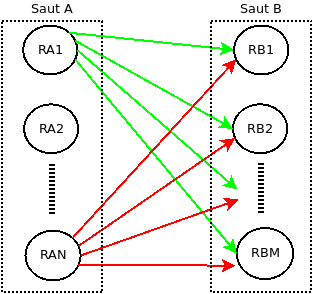
\includegraphics[width=0.5\linewidth]{illustrations/link-inference}
		% Graphic for TeX using PGF
% Title: /home/hayat/RipeAtlasTraceroutesAnalysis/report/illustrations/link-inference.dia
% Creator: Dia v0.97+git
% CreationDate: Thu Nov 29 20:58:09 2018
% For: hayat
% \usepackage{tikz}
% The following commands are not supported in PSTricks at present
% We define them conditionally, so when they are implemented,
% this pgf file will use them.
\ifx\du\undefined
  \newlength{\du}
\fi
\setlength{\du}{15\unitlength}
\begin{tikzpicture}[even odd rule]
\pgftransformxscale{1.000000}
\pgftransformyscale{-1.000000}
\definecolor{dialinecolor}{rgb}{0.000000, 0.000000, 0.000000}
\pgfsetstrokecolor{dialinecolor}
\pgfsetstrokeopacity{1.000000}
\definecolor{diafillcolor}{rgb}{1.000000, 1.000000, 1.000000}
\pgfsetfillcolor{diafillcolor}
\pgfsetfillopacity{1.000000}
\pgfsetlinewidth{0.100000\du}
\pgfsetdash{}{0pt}
\pgfsetmiterjoin
\definecolor{diafillcolor}{rgb}{1.000000, 1.000000, 1.000000}
\pgfsetfillcolor{diafillcolor}
\pgfsetfillopacity{1.000000}
\pgfpathellipse{\pgfpoint{27.430614\du}{13.298442\du}}{\pgfpoint{1.349214\du}{0\du}}{\pgfpoint{0\du}{1.217042\du}}
\pgfusepath{fill}
\definecolor{dialinecolor}{rgb}{0.000000, 0.000000, 0.000000}
\pgfsetstrokecolor{dialinecolor}
\pgfsetstrokeopacity{1.000000}
\pgfpathellipse{\pgfpoint{27.430614\du}{13.298442\du}}{\pgfpoint{1.349214\du}{0\du}}{\pgfpoint{0\du}{1.217042\du}}
\pgfusepath{stroke}
% setfont left to latex
\definecolor{dialinecolor}{rgb}{0.000000, 0.000000, 0.000000}
\pgfsetstrokecolor{dialinecolor}
\pgfsetstrokeopacity{1.000000}
\definecolor{diafillcolor}{rgb}{0.000000, 0.000000, 0.000000}
\pgfsetfillcolor{diafillcolor}
\pgfsetfillopacity{1.000000}
\node[anchor=base,inner sep=0pt, outer sep=0pt,color=dialinecolor] at (27.430614\du,13.493442\du){$R_{1,1}$};
\pgfsetlinewidth{0.100000\du}
\pgfsetdash{}{0pt}
\pgfsetmiterjoin
\definecolor{diafillcolor}{rgb}{1.000000, 1.000000, 1.000000}
\pgfsetfillcolor{diafillcolor}
\pgfsetfillopacity{1.000000}
\pgfpathellipse{\pgfpoint{27.475614\du}{17.238442\du}}{\pgfpoint{1.349214\du}{0\du}}{\pgfpoint{0\du}{1.217042\du}}
\pgfusepath{fill}
\definecolor{dialinecolor}{rgb}{0.000000, 0.000000, 0.000000}
\pgfsetstrokecolor{dialinecolor}
\pgfsetstrokeopacity{1.000000}
\pgfpathellipse{\pgfpoint{27.475614\du}{17.238442\du}}{\pgfpoint{1.349214\du}{0\du}}{\pgfpoint{0\du}{1.217042\du}}
\pgfusepath{stroke}
% setfont left to latex
\definecolor{dialinecolor}{rgb}{0.000000, 0.000000, 0.000000}
\pgfsetstrokecolor{dialinecolor}
\pgfsetstrokeopacity{1.000000}
\definecolor{diafillcolor}{rgb}{0.000000, 0.000000, 0.000000}
\pgfsetfillcolor{diafillcolor}
\pgfsetfillopacity{1.000000}
\node[anchor=base,inner sep=0pt, outer sep=0pt,color=dialinecolor] at (27.475614\du,17.433442\du){$R_{1,2}$};
\pgfsetlinewidth{0.100000\du}
\pgfsetdash{}{0pt}
\pgfsetmiterjoin
\definecolor{diafillcolor}{rgb}{1.000000, 1.000000, 1.000000}
\pgfsetfillcolor{diafillcolor}
\pgfsetfillopacity{1.000000}
\pgfpathellipse{\pgfpoint{27.570578\du}{23.578496\du}}{\pgfpoint{1.376878\du}{0\du}}{\pgfpoint{0\du}{1.241996\du}}
\pgfusepath{fill}
\definecolor{dialinecolor}{rgb}{0.000000, 0.000000, 0.000000}
\pgfsetstrokecolor{dialinecolor}
\pgfsetstrokeopacity{1.000000}
\pgfpathellipse{\pgfpoint{27.570578\du}{23.578496\du}}{\pgfpoint{1.376878\du}{0\du}}{\pgfpoint{0\du}{1.241996\du}}
\pgfusepath{stroke}
% setfont left to latex
\definecolor{dialinecolor}{rgb}{0.000000, 0.000000, 0.000000}
\pgfsetstrokecolor{dialinecolor}
\pgfsetstrokeopacity{1.000000}
\definecolor{diafillcolor}{rgb}{0.000000, 0.000000, 0.000000}
\pgfsetfillcolor{diafillcolor}
\pgfsetfillopacity{1.000000}
\node[anchor=base,inner sep=0pt, outer sep=0pt,color=dialinecolor] at (27.570578\du,23.773496\du){$R_{1,N}$};
\pgfsetlinewidth{0.300000\du}
\pgfsetdash{{\pgflinewidth}{0.200000\du}}{0cm}
\pgfsetbuttcap
{
\definecolor{diafillcolor}{rgb}{0.000000, 0.000000, 0.000000}
\pgfsetfillcolor{diafillcolor}
\pgfsetfillopacity{1.000000}
% was here!!!
\definecolor{dialinecolor}{rgb}{0.000000, 0.000000, 0.000000}
\pgfsetstrokecolor{dialinecolor}
\pgfsetstrokeopacity{1.000000}
\draw (27.540000\du,18.980000\du)--(27.540000\du,21.480000\du);
}
\pgfsetlinewidth{0.100000\du}
\pgfsetdash{}{0pt}
\pgfsetmiterjoin
\definecolor{diafillcolor}{rgb}{1.000000, 1.000000, 1.000000}
\pgfsetfillcolor{diafillcolor}
\pgfsetfillopacity{1.000000}
\pgfpathellipse{\pgfpoint{37.980536\du}{13.298484\du}}{\pgfpoint{1.355136\du}{0\du}}{\pgfpoint{0\du}{1.222384\du}}
\pgfusepath{fill}
\definecolor{dialinecolor}{rgb}{0.000000, 0.000000, 0.000000}
\pgfsetstrokecolor{dialinecolor}
\pgfsetstrokeopacity{1.000000}
\pgfpathellipse{\pgfpoint{37.980536\du}{13.298484\du}}{\pgfpoint{1.355136\du}{0\du}}{\pgfpoint{0\du}{1.222384\du}}
\pgfusepath{stroke}
% setfont left to latex
\definecolor{dialinecolor}{rgb}{0.000000, 0.000000, 0.000000}
\pgfsetstrokecolor{dialinecolor}
\pgfsetstrokeopacity{1.000000}
\definecolor{diafillcolor}{rgb}{0.000000, 0.000000, 0.000000}
\pgfsetfillcolor{diafillcolor}
\pgfsetfillopacity{1.000000}
\node[anchor=base,inner sep=0pt, outer sep=0pt,color=dialinecolor] at (37.980536\du,13.493484\du){$R_{2,1}$};
\pgfsetlinewidth{0.100000\du}
\pgfsetdash{}{0pt}
\pgfsetmiterjoin
\definecolor{diafillcolor}{rgb}{1.000000, 1.000000, 1.000000}
\pgfsetfillcolor{diafillcolor}
\pgfsetfillopacity{1.000000}
\pgfpathellipse{\pgfpoint{37.925536\du}{17.238484\du}}{\pgfpoint{1.355136\du}{0\du}}{\pgfpoint{0\du}{1.222384\du}}
\pgfusepath{fill}
\definecolor{dialinecolor}{rgb}{0.000000, 0.000000, 0.000000}
\pgfsetstrokecolor{dialinecolor}
\pgfsetstrokeopacity{1.000000}
\pgfpathellipse{\pgfpoint{37.925536\du}{17.238484\du}}{\pgfpoint{1.355136\du}{0\du}}{\pgfpoint{0\du}{1.222384\du}}
\pgfusepath{stroke}
% setfont left to latex
\definecolor{dialinecolor}{rgb}{0.000000, 0.000000, 0.000000}
\pgfsetstrokecolor{dialinecolor}
\pgfsetstrokeopacity{1.000000}
\definecolor{diafillcolor}{rgb}{0.000000, 0.000000, 0.000000}
\pgfsetfillcolor{diafillcolor}
\pgfsetfillopacity{1.000000}
\node[anchor=base,inner sep=0pt, outer sep=0pt,color=dialinecolor] at (37.925536\du,17.433484\du){$R_{2,2}$};
\pgfsetlinewidth{0.100000\du}
\pgfsetdash{}{0pt}
\pgfsetmiterjoin
\definecolor{diafillcolor}{rgb}{1.000000, 1.000000, 1.000000}
\pgfsetfillcolor{diafillcolor}
\pgfsetfillopacity{1.000000}
\pgfpathellipse{\pgfpoint{38.170599\du}{23.478445\du}}{\pgfpoint{1.411299\du}{0\du}}{\pgfpoint{0\du}{1.273045\du}}
\pgfusepath{fill}
\definecolor{dialinecolor}{rgb}{0.000000, 0.000000, 0.000000}
\pgfsetstrokecolor{dialinecolor}
\pgfsetstrokeopacity{1.000000}
\pgfpathellipse{\pgfpoint{38.170599\du}{23.478445\du}}{\pgfpoint{1.411299\du}{0\du}}{\pgfpoint{0\du}{1.273045\du}}
\pgfusepath{stroke}
% setfont left to latex
\definecolor{dialinecolor}{rgb}{0.000000, 0.000000, 0.000000}
\pgfsetstrokecolor{dialinecolor}
\pgfsetstrokeopacity{1.000000}
\definecolor{diafillcolor}{rgb}{0.000000, 0.000000, 0.000000}
\pgfsetfillcolor{diafillcolor}
\pgfsetfillopacity{1.000000}
\node[anchor=base,inner sep=0pt, outer sep=0pt,color=dialinecolor] at (38.170599\du,23.673445\du){$R_{1,M}$};
\pgfsetlinewidth{0.300000\du}
\pgfsetdash{{\pgflinewidth}{0.200000\du}}{0cm}
\pgfsetbuttcap
{
\definecolor{diafillcolor}{rgb}{0.000000, 0.000000, 0.000000}
\pgfsetfillcolor{diafillcolor}
\pgfsetfillopacity{1.000000}
% was here!!!
\definecolor{dialinecolor}{rgb}{0.000000, 0.000000, 0.000000}
\pgfsetstrokecolor{dialinecolor}
\pgfsetstrokeopacity{1.000000}
\draw (37.985000\du,18.970000\du)--(37.985000\du,21.470000\du);
}
\pgfsetlinewidth{0.050000\du}
\pgfsetdash{}{0pt}
\pgfsetbuttcap
{
\definecolor{diafillcolor}{rgb}{0.000000, 1.000000, 0.000000}
\pgfsetfillcolor{diafillcolor}
\pgfsetfillopacity{1.000000}
% was here!!!
\pgfsetarrowsstart{stealth}
\definecolor{dialinecolor}{rgb}{0.000000, 1.000000, 0.000000}
\pgfsetstrokecolor{dialinecolor}
\pgfsetstrokeopacity{1.000000}
\draw (28.384600\du,12.437900\du)--(37.022310\du,12.434128\du);
}
\pgfsetlinewidth{0.050000\du}
\pgfsetdash{}{0pt}
\pgfsetbuttcap
{
\definecolor{diafillcolor}{rgb}{1.000000, 0.000000, 0.000000}
\pgfsetfillcolor{diafillcolor}
\pgfsetfillopacity{1.000000}
% was here!!!
\pgfsetarrowsstart{stealth}
\definecolor{dialinecolor}{rgb}{1.000000, 0.000000, 0.000000}
\pgfsetstrokecolor{dialinecolor}
\pgfsetstrokeopacity{1.000000}
\draw (28.842600\du,24.053700\du)--(37.630518\du,24.654584\du);
}
\pgfsetlinewidth{0.100000\du}
\pgfsetdash{{\pgflinewidth}{0.200000\du}}{0cm}
\pgfsetmiterjoin
\pgfsetbuttcap
{\pgfsetcornersarced{\pgfpoint{0.000000\du}{0.000000\du}}\definecolor{dialinecolor}{rgb}{0.000000, 0.000000, 0.000000}
\pgfsetstrokecolor{dialinecolor}
\pgfsetstrokeopacity{1.000000}
\draw (25.638764\du,11.830038\du)--(25.638764\du,25.156536\du)--(29.721269\du,25.156536\du)--(29.721269\du,11.830038\du)--cycle;
}\pgfsetlinewidth{0.100000\du}
\pgfsetdash{{\pgflinewidth}{0.200000\du}}{0cm}
\pgfsetmiterjoin
\pgfsetbuttcap
{\pgfsetcornersarced{\pgfpoint{0.000000\du}{0.000000\du}}\definecolor{dialinecolor}{rgb}{0.000000, 0.000000, 0.000000}
\pgfsetstrokecolor{dialinecolor}
\pgfsetstrokeopacity{1.000000}
\draw (36.096688\du,11.857262\du)--(36.096688\du,25.128574\du)--(39.871607\du,25.128574\du)--(39.871607\du,11.857262\du)--cycle;
}% setfont left to latex
\definecolor{dialinecolor}{rgb}{0.000000, 0.000000, 0.000000}
\pgfsetstrokecolor{dialinecolor}
\pgfsetstrokeopacity{1.000000}
\definecolor{diafillcolor}{rgb}{0.000000, 0.000000, 0.000000}
\pgfsetfillcolor{diafillcolor}
\pgfsetfillopacity{1.000000}
\node[anchor=base west,inner sep=0pt,outer sep=0pt,color=dialinecolor] at (26.470600\du,11.464400\du){$ h_1 $};
% setfont left to latex
\definecolor{dialinecolor}{rgb}{0.000000, 0.000000, 0.000000}
\pgfsetstrokecolor{dialinecolor}
\pgfsetstrokeopacity{1.000000}
\definecolor{diafillcolor}{rgb}{0.000000, 0.000000, 0.000000}
\pgfsetfillcolor{diafillcolor}
\pgfsetfillopacity{1.000000}
\node[anchor=base west,inner sep=0pt,outer sep=0pt,color=dialinecolor] at (36.898700\du,11.464100\du){$ h_2 $};
\pgfsetlinewidth{0.050000\du}
\pgfsetdash{}{0pt}
\pgfsetbuttcap
{
\definecolor{diafillcolor}{rgb}{0.000000, 0.000000, 1.000000}
\pgfsetfillcolor{diafillcolor}
\pgfsetfillopacity{1.000000}
% was here!!!
\pgfsetarrowsstart{stealth}
\definecolor{dialinecolor}{rgb}{0.000000, 0.000000, 1.000000}
\pgfsetstrokecolor{dialinecolor}
\pgfsetstrokeopacity{1.000000}
\draw (28.779828\du,13.298442\du)--(37.406948\du,16.109148\du);
}
\pgfsetlinewidth{0.050000\du}
\pgfsetdash{}{0pt}
\pgfsetbuttcap
{
\definecolor{diafillcolor}{rgb}{0.000000, 1.000000, 0.000000}
\pgfsetfillcolor{diafillcolor}
\pgfsetfillopacity{1.000000}
% was here!!!
\pgfsetarrowsstart{stealth}
\definecolor{dialinecolor}{rgb}{0.000000, 1.000000, 0.000000}
\pgfsetstrokecolor{dialinecolor}
\pgfsetstrokeopacity{1.000000}
\draw (28.722125\du,16.772700\du)--(36.728554\du,12.830698\du);
}
\pgfsetlinewidth{0.050000\du}
\pgfsetdash{}{0pt}
\pgfsetbuttcap
{
\definecolor{diafillcolor}{rgb}{0.000000, 1.000000, 0.000000}
\pgfsetfillcolor{diafillcolor}
\pgfsetfillopacity{1.000000}
% was here!!!
\pgfsetarrowsstart{stealth}
\definecolor{dialinecolor}{rgb}{0.000000, 1.000000, 0.000000}
\pgfsetstrokecolor{dialinecolor}
\pgfsetstrokeopacity{1.000000}
\draw (28.602774\du,20.095348\du)--(36.625400\du,13.298484\du);
}
\pgfsetlinewidth{0.050000\du}
\pgfsetdash{}{0pt}
\pgfsetbuttcap
{
\definecolor{diafillcolor}{rgb}{0.000000, 1.000000, 0.000000}
\pgfsetfillcolor{diafillcolor}
\pgfsetfillopacity{1.000000}
% was here!!!
\pgfsetarrowsstart{stealth}
\definecolor{dialinecolor}{rgb}{0.000000, 1.000000, 0.000000}
\pgfsetstrokecolor{dialinecolor}
\pgfsetstrokeopacity{1.000000}
\draw (28.097487\du,22.431041\du)--(36.728554\du,13.766270\du);
}
\pgfsetlinewidth{0.050000\du}
\pgfsetdash{}{0pt}
\pgfsetbuttcap
{
\definecolor{diafillcolor}{rgb}{0.000000, 0.000000, 1.000000}
\pgfsetfillcolor{diafillcolor}
\pgfsetfillopacity{1.000000}
% was here!!!
\pgfsetarrowsstart{stealth}
\definecolor{dialinecolor}{rgb}{0.000000, 0.000000, 1.000000}
\pgfsetstrokecolor{dialinecolor}
\pgfsetstrokeopacity{1.000000}
\draw (28.824828\du,17.238442\du)--(36.967310\du,16.374128\du);
}
\pgfsetlinewidth{0.050000\du}
\pgfsetdash{}{0pt}
\pgfsetbuttcap
{
\definecolor{diafillcolor}{rgb}{0.000000, 0.000000, 1.000000}
\pgfsetfillcolor{diafillcolor}
\pgfsetfillopacity{1.000000}
% was here!!!
\pgfsetarrowsstart{stealth}
\definecolor{dialinecolor}{rgb}{0.000000, 0.000000, 1.000000}
\pgfsetstrokecolor{dialinecolor}
\pgfsetstrokeopacity{1.000000}
\draw (28.798511\du,20.486821\du)--(36.673554\du,16.770698\du);
}
\pgfsetlinewidth{0.050000\du}
\pgfsetdash{}{0pt}
\pgfsetbuttcap
{
\definecolor{diafillcolor}{rgb}{0.000000, 0.000000, 1.000000}
\pgfsetfillcolor{diafillcolor}
\pgfsetfillopacity{1.000000}
% was here!!!
\pgfsetarrowsstart{stealth}
\definecolor{dialinecolor}{rgb}{0.000000, 0.000000, 1.000000}
\pgfsetstrokecolor{dialinecolor}
\pgfsetstrokeopacity{1.000000}
\draw (28.544178\du,22.700272\du)--(36.516123\du,17.355037\du);
}
\pgfsetlinewidth{0.050000\du}
\pgfsetdash{}{0pt}
\pgfsetbuttcap
{
\definecolor{diafillcolor}{rgb}{1.000000, 0.000000, 0.000000}
\pgfsetfillcolor{diafillcolor}
\pgfsetfillopacity{1.000000}
% was here!!!
\pgfsetarrowsstart{stealth}
\definecolor{dialinecolor}{rgb}{1.000000, 0.000000, 0.000000}
\pgfsetstrokecolor{dialinecolor}
\pgfsetstrokeopacity{1.000000}
\draw (28.938323\du,20.850332\du)--(36.866729\du,23.965618\du);
}
\pgfsetlinewidth{0.050000\du}
\pgfsetdash{}{0pt}
\pgfsetbuttcap
{
\definecolor{diafillcolor}{rgb}{1.000000, 0.000000, 0.000000}
\pgfsetfillcolor{diafillcolor}
\pgfsetfillopacity{1.000000}
% was here!!!
\pgfsetarrowsstart{stealth}
\definecolor{dialinecolor}{rgb}{1.000000, 0.000000, 0.000000}
\pgfsetstrokecolor{dialinecolor}
\pgfsetstrokeopacity{1.000000}
\draw (28.722125\du,17.704183\du)--(36.712688\du,23.381227\du);
}
\pgfsetlinewidth{0.050000\du}
\pgfsetdash{}{0pt}
\pgfsetbuttcap
{
\definecolor{diafillcolor}{rgb}{1.000000, 0.000000, 0.000000}
\pgfsetfillcolor{diafillcolor}
\pgfsetfillopacity{1.000000}
% was here!!!
\pgfsetarrowsstart{stealth}
\definecolor{dialinecolor}{rgb}{1.000000, 0.000000, 0.000000}
\pgfsetstrokecolor{dialinecolor}
\pgfsetstrokeopacity{1.000000}
\draw (28.677125\du,13.764183\du)--(36.866729\du,22.991272\du);
}
\end{tikzpicture}

	}
	\caption{Inférence des liens possibles entre les routeurs des deux sauts $h_{1}$ et $h_{2}$}
	\label{fig:link-inference_}
\end{figure}
\paragraph{5. Calcul des RTTs différentiels des liens.}  A cette étape, on calcule le RTT différentiel de chaque  lien, parmi les liens obtenus de l'étape $4$, en calculant la différence entre les RTTs des deux routeurs impliqués dans le  lien en question (équation \ref{eq:rttdifference}). En plus du RTT différentiel, on note aussi la sonde  ayant effectué la requête traceroute où le lien a été identifié. 

%A l'issue de cette étape, pour tout traceroute, on obtient la liste des liens possibles tout en reprenant des informations générales de la requête traceroute comme le temps de la requête (timestamp), etc.

\paragraph{6. Fusion des informations d'un lien.} Un lien (IP1, IP2) peut être identifié plusieurs fois pendant une même période $d_k$. De plus, d'après le travail de référence,  le lien (IP2, IP1) est similaire au lien  (IP1, IP2). La fusion permet de construire une nouvelle distribution des RTTs différentiels caractérisant le lien (IP1, IP2) qui reprend les RTTs différentiels du lien (IP1, IP2) ainsi que ceux du lien (IP2, IP1). La similarité de deux liens  implique que les RTTs différentiels qui caractérisent un lien (IP2, IP1) caractérisent aussi le lien (IP1, IP2), d'où la fusion effectuée.


A la fin de l'étape 6, tous les traceroutes sont préparés. A présent, l'objectif est d'identifier les dates pendant lesquelles des anomalies ont été détectées. Pour ce faire, l'idée du travail de référence est de conserver, pour un lien donné, une référence du RTT différentiel médian.  Cette référence est d'abord comparée avec la médiane courante des RTTs différentiels,  puis,  mise à jour au fur et à mesure   tout au long de la période de l'analyse. A cette médiane, un intervalle de confiance est associé. Ainsi, l'intervalle de confiance fait partie aussi de la référence du lien. 


\paragraph{7. Calcul de la médiane des RTTs différentiels et  de son intervalle de confiance courants.} Pour un lien donné, on calcule la médiane des RTTs différentiels d'une période $d_k$, ensuite on calcule les deux bornes de l'intervalle de confiance  courant de cette médiane pour $d_k$.  


\paragraph{8. Mise à jour de la médiane  des RTTs différentiels et de son intervalle  de confiance de  référence.} La médiane des RTTs différentiels de référence ainsi que l'intervalle de confiance de référence sont mise à jour tant que la période déclenchant la détection des anomalies n'est pas atteinte.  La mise à jour de la référence : médiane et les bornes de l'intervalle de confiance se base sur la moyenne mobile exponentielle. Cette méthode prend en compte les valeurs antérieures ainsi que celles récentes en étant dirigée par le paramètre \textit{confInterval} décrit dans la section \ref{par:parametre-de-lanalyse}.


\paragraph{9. Comparaison des intervalles de confiance  des RTTs différentiels : courant et référence.} 

La comparaison de l'état courant du lien avec celui de référence est effectuée en analysant le chevauchement d'intervalles de confiance  courant et de référence.  Soient 
 \textit{referenceCiLow} et \textit{referenceCiHight} sont les bornes de l'intervalle de confiance de référence.  \textit{currentCiLow} et \textit{currentCiHight} sont les bornes de l'intervalle de confiance courant.

%Le délai d'un lien est jugé normal si son intervalle de confiance courant est inclus dans l'intervalle de confiance de référence. C'est le cas $1$ dans 
%, 
%D'après le travail de référence, on distingue quatre cas possibles  illustrés dans la Figure 	\ref{fig:intervals-comparaison}:
La Figure 	\ref{fig:intervals-comparaison} représente des cas possibles de positionnement des deux intervalles de confiance.

\textbf{Cas 1 :} le délai du lien est normal.

\textbf{Cas 2 :} le délai du lien est anormal.

\textbf{Cas 3 :} le délai du lien est normal.

\textbf{Cas 4 :} le délai du lien est normal.

\textbf{Cas 5 :} le délai du lien est anormal.

\textbf{Cas 6 :} le délai du lien est anormal.


\begin{figure}[h]
	\centering
	\captionsetup{justification=centering}
	\resizebox{\textwidth}{!}{
		% Graphic for TeX using PGF
% Title: /home/hayat/RipeAtlasTraceroutesAnalysis/2019/Rapport_Mai/illustrations/intervals-comparaison.dia
% Creator: Dia v0.97+git
% CreationDate: Wed May 22 04:02:45 2019
% For: hayat
% \usepackage{tikz}
% The following commands are not supported in PSTricks at present
% We define them conditionally, so when they are implemented,
% this pgf file will use them.
\ifx\du\undefined
  \newlength{\du}
\fi
\setlength{\du}{15\unitlength}
\begin{tikzpicture}[even odd rule]
\pgftransformxscale{1.000000}
\pgftransformyscale{-1.000000}
\definecolor{dialinecolor}{rgb}{0.000000, 0.000000, 0.000000}
\pgfsetstrokecolor{dialinecolor}
\pgfsetstrokeopacity{1.000000}
\definecolor{diafillcolor}{rgb}{1.000000, 1.000000, 1.000000}
\pgfsetfillcolor{diafillcolor}
\pgfsetfillopacity{1.000000}
\pgfsetlinewidth{0.100000\du}
\pgfsetdash{}{0pt}
\pgfsetbuttcap
{
\definecolor{diafillcolor}{rgb}{0.662745, 0.709804, 0.674510}
\pgfsetfillcolor{diafillcolor}
\pgfsetfillopacity{1.000000}
% was here!!!
}
\definecolor{dialinecolor}{rgb}{0.662745, 0.709804, 0.674510}
\pgfsetstrokecolor{dialinecolor}
\pgfsetstrokeopacity{1.000000}
\draw (14.150000\du,0.400000\du)--(27.000000\du,0.400000\du);
\pgfsetlinewidth{0.100000\du}
\pgfsetdash{}{0pt}
\pgfsetmiterjoin
\pgfsetbuttcap
\definecolor{diafillcolor}{rgb}{0.662745, 0.709804, 0.674510}
\pgfsetfillcolor{diafillcolor}
\pgfsetfillopacity{1.000000}
\fill (13.900000\du,0.550000\du)--(13.900000\du,0.250000\du)--(14.200000\du,0.250000\du)--(14.200000\du,0.550000\du)--cycle;
\definecolor{dialinecolor}{rgb}{0.662745, 0.709804, 0.674510}
\pgfsetstrokecolor{dialinecolor}
\pgfsetstrokeopacity{1.000000}
\draw (14.050000\du,0.700000\du)--(14.050000\du,0.100000\du);
\pgfsetlinewidth{0.100000\du}
\pgfsetdash{}{0pt}
\pgfsetmiterjoin
\pgfsetbuttcap
\definecolor{diafillcolor}{rgb}{0.662745, 0.709804, 0.674510}
\pgfsetfillcolor{diafillcolor}
\pgfsetfillopacity{1.000000}
\fill (27.250000\du,0.250000\du)--(27.250000\du,0.550000\du)--(26.950000\du,0.550000\du)--(26.950000\du,0.250000\du)--cycle;
\definecolor{dialinecolor}{rgb}{0.662745, 0.709804, 0.674510}
\pgfsetstrokecolor{dialinecolor}
\pgfsetstrokeopacity{1.000000}
\draw (27.100000\du,0.100000\du)--(27.100000\du,0.700000\du);
\pgfsetlinewidth{0.100000\du}
\pgfsetdash{}{0pt}
\pgfsetbuttcap
{
\definecolor{diafillcolor}{rgb}{0.000000, 0.000000, 0.000000}
\pgfsetfillcolor{diafillcolor}
\pgfsetfillopacity{1.000000}
% was here!!!
}
\definecolor{dialinecolor}{rgb}{0.000000, 0.000000, 0.000000}
\pgfsetstrokecolor{dialinecolor}
\pgfsetstrokeopacity{1.000000}
\draw (16.150000\du,2.450000\du)--(24.800000\du,2.450000\du);
\pgfsetlinewidth{0.100000\du}
\pgfsetdash{}{0pt}
\pgfsetmiterjoin
\pgfsetbuttcap
\definecolor{diafillcolor}{rgb}{0.000000, 0.000000, 0.000000}
\pgfsetfillcolor{diafillcolor}
\pgfsetfillopacity{1.000000}
\fill (15.900000\du,2.600000\du)--(15.900000\du,2.300000\du)--(16.200000\du,2.300000\du)--(16.200000\du,2.600000\du)--cycle;
\definecolor{dialinecolor}{rgb}{0.000000, 0.000000, 0.000000}
\pgfsetstrokecolor{dialinecolor}
\pgfsetstrokeopacity{1.000000}
\draw (16.050000\du,2.750000\du)--(16.050000\du,2.150000\du);
\pgfsetlinewidth{0.100000\du}
\pgfsetdash{}{0pt}
\pgfsetmiterjoin
\pgfsetbuttcap
\definecolor{diafillcolor}{rgb}{0.000000, 0.000000, 0.000000}
\pgfsetfillcolor{diafillcolor}
\pgfsetfillopacity{1.000000}
\fill (25.050000\du,2.300000\du)--(25.050000\du,2.600000\du)--(24.750000\du,2.600000\du)--(24.750000\du,2.300000\du)--cycle;
\definecolor{dialinecolor}{rgb}{0.000000, 0.000000, 0.000000}
\pgfsetstrokecolor{dialinecolor}
\pgfsetstrokeopacity{1.000000}
\draw (24.900000\du,2.150000\du)--(24.900000\du,2.750000\du);
\pgfsetlinewidth{0.100000\du}
\pgfsetdash{}{0pt}
\pgfsetbuttcap
{
\definecolor{diafillcolor}{rgb}{0.662745, 0.709804, 0.674510}
\pgfsetfillcolor{diafillcolor}
\pgfsetfillopacity{1.000000}
% was here!!!
}
\definecolor{dialinecolor}{rgb}{0.662745, 0.709804, 0.674510}
\pgfsetstrokecolor{dialinecolor}
\pgfsetstrokeopacity{1.000000}
\draw (14.008200\du,11.548100\du)--(26.858200\du,11.548100\du);
\pgfsetlinewidth{0.100000\du}
\pgfsetdash{}{0pt}
\pgfsetmiterjoin
\pgfsetbuttcap
\definecolor{diafillcolor}{rgb}{0.662745, 0.709804, 0.674510}
\pgfsetfillcolor{diafillcolor}
\pgfsetfillopacity{1.000000}
\fill (13.758200\du,11.698100\du)--(13.758200\du,11.398100\du)--(14.058200\du,11.398100\du)--(14.058200\du,11.698100\du)--cycle;
\definecolor{dialinecolor}{rgb}{0.662745, 0.709804, 0.674510}
\pgfsetstrokecolor{dialinecolor}
\pgfsetstrokeopacity{1.000000}
\draw (13.908200\du,11.848100\du)--(13.908200\du,11.248100\du);
\pgfsetlinewidth{0.100000\du}
\pgfsetdash{}{0pt}
\pgfsetmiterjoin
\pgfsetbuttcap
\definecolor{diafillcolor}{rgb}{0.662745, 0.709804, 0.674510}
\pgfsetfillcolor{diafillcolor}
\pgfsetfillopacity{1.000000}
\fill (27.108200\du,11.398100\du)--(27.108200\du,11.698100\du)--(26.808200\du,11.698100\du)--(26.808200\du,11.398100\du)--cycle;
\definecolor{dialinecolor}{rgb}{0.662745, 0.709804, 0.674510}
\pgfsetstrokecolor{dialinecolor}
\pgfsetstrokeopacity{1.000000}
\draw (26.958200\du,11.248100\du)--(26.958200\du,11.848100\du);
\pgfsetlinewidth{0.100000\du}
\pgfsetdash{}{0pt}
\pgfsetbuttcap
{
\definecolor{diafillcolor}{rgb}{0.000000, 0.000000, 0.000000}
\pgfsetfillcolor{diafillcolor}
\pgfsetfillopacity{1.000000}
% was here!!!
}
\definecolor{dialinecolor}{rgb}{0.000000, 0.000000, 0.000000}
\pgfsetstrokecolor{dialinecolor}
\pgfsetstrokeopacity{1.000000}
\draw (23.108200\du,13.598100\du)--(31.758200\du,13.598100\du);
\pgfsetlinewidth{0.100000\du}
\pgfsetdash{}{0pt}
\pgfsetmiterjoin
\pgfsetbuttcap
\definecolor{diafillcolor}{rgb}{0.000000, 0.000000, 0.000000}
\pgfsetfillcolor{diafillcolor}
\pgfsetfillopacity{1.000000}
\fill (22.858200\du,13.748100\du)--(22.858200\du,13.448100\du)--(23.158200\du,13.448100\du)--(23.158200\du,13.748100\du)--cycle;
\definecolor{dialinecolor}{rgb}{0.000000, 0.000000, 0.000000}
\pgfsetstrokecolor{dialinecolor}
\pgfsetstrokeopacity{1.000000}
\draw (23.008200\du,13.898100\du)--(23.008200\du,13.298100\du);
\pgfsetlinewidth{0.100000\du}
\pgfsetdash{}{0pt}
\pgfsetmiterjoin
\pgfsetbuttcap
\definecolor{diafillcolor}{rgb}{0.000000, 0.000000, 0.000000}
\pgfsetfillcolor{diafillcolor}
\pgfsetfillopacity{1.000000}
\fill (32.008200\du,13.448100\du)--(32.008200\du,13.748100\du)--(31.708200\du,13.748100\du)--(31.708200\du,13.448100\du)--cycle;
\definecolor{dialinecolor}{rgb}{0.000000, 0.000000, 0.000000}
\pgfsetstrokecolor{dialinecolor}
\pgfsetstrokeopacity{1.000000}
\draw (31.858200\du,13.298100\du)--(31.858200\du,13.898100\du);
\pgfsetlinewidth{0.100000\du}
\pgfsetdash{}{0pt}
\pgfsetbuttcap
{
\definecolor{diafillcolor}{rgb}{0.662745, 0.709804, 0.674510}
\pgfsetfillcolor{diafillcolor}
\pgfsetfillopacity{1.000000}
% was here!!!
}
\definecolor{dialinecolor}{rgb}{0.662745, 0.709804, 0.674510}
\pgfsetstrokecolor{dialinecolor}
\pgfsetstrokeopacity{1.000000}
\draw (14.108200\du,17.048100\du)--(26.958200\du,17.048100\du);
\pgfsetlinewidth{0.100000\du}
\pgfsetdash{}{0pt}
\pgfsetmiterjoin
\pgfsetbuttcap
\definecolor{diafillcolor}{rgb}{0.662745, 0.709804, 0.674510}
\pgfsetfillcolor{diafillcolor}
\pgfsetfillopacity{1.000000}
\fill (13.858200\du,17.198100\du)--(13.858200\du,16.898100\du)--(14.158200\du,16.898100\du)--(14.158200\du,17.198100\du)--cycle;
\definecolor{dialinecolor}{rgb}{0.662745, 0.709804, 0.674510}
\pgfsetstrokecolor{dialinecolor}
\pgfsetstrokeopacity{1.000000}
\draw (14.008200\du,17.348100\du)--(14.008200\du,16.748100\du);
\pgfsetlinewidth{0.100000\du}
\pgfsetdash{}{0pt}
\pgfsetmiterjoin
\pgfsetbuttcap
\definecolor{diafillcolor}{rgb}{0.662745, 0.709804, 0.674510}
\pgfsetfillcolor{diafillcolor}
\pgfsetfillopacity{1.000000}
\fill (27.208200\du,16.898100\du)--(27.208200\du,17.198100\du)--(26.908200\du,17.198100\du)--(26.908200\du,16.898100\du)--cycle;
\definecolor{dialinecolor}{rgb}{0.662745, 0.709804, 0.674510}
\pgfsetstrokecolor{dialinecolor}
\pgfsetstrokeopacity{1.000000}
\draw (27.058200\du,16.748100\du)--(27.058200\du,17.348100\du);
\pgfsetlinewidth{0.100000\du}
\pgfsetdash{}{0pt}
\pgfsetbuttcap
{
\definecolor{diafillcolor}{rgb}{0.000000, 0.000000, 0.000000}
\pgfsetfillcolor{diafillcolor}
\pgfsetfillopacity{1.000000}
% was here!!!
}
\definecolor{dialinecolor}{rgb}{0.000000, 0.000000, 0.000000}
\pgfsetstrokecolor{dialinecolor}
\pgfsetstrokeopacity{1.000000}
\draw (9.308250\du,19.048100\du)--(17.958200\du,19.048100\du);
\pgfsetlinewidth{0.100000\du}
\pgfsetdash{}{0pt}
\pgfsetmiterjoin
\pgfsetbuttcap
\definecolor{diafillcolor}{rgb}{0.000000, 0.000000, 0.000000}
\pgfsetfillcolor{diafillcolor}
\pgfsetfillopacity{1.000000}
\fill (9.058250\du,19.198100\du)--(9.058250\du,18.898100\du)--(9.358250\du,18.898100\du)--(9.358250\du,19.198100\du)--cycle;
\definecolor{dialinecolor}{rgb}{0.000000, 0.000000, 0.000000}
\pgfsetstrokecolor{dialinecolor}
\pgfsetstrokeopacity{1.000000}
\draw (9.208250\du,19.348100\du)--(9.208250\du,18.748100\du);
\pgfsetlinewidth{0.100000\du}
\pgfsetdash{}{0pt}
\pgfsetmiterjoin
\pgfsetbuttcap
\definecolor{diafillcolor}{rgb}{0.000000, 0.000000, 0.000000}
\pgfsetfillcolor{diafillcolor}
\pgfsetfillopacity{1.000000}
\fill (18.208200\du,18.898100\du)--(18.208200\du,19.198100\du)--(17.908200\du,19.198100\du)--(17.908200\du,18.898100\du)--cycle;
\definecolor{dialinecolor}{rgb}{0.000000, 0.000000, 0.000000}
\pgfsetstrokecolor{dialinecolor}
\pgfsetstrokeopacity{1.000000}
\draw (18.058200\du,18.748100\du)--(18.058200\du,19.348100\du);
\pgfsetlinewidth{0.100000\du}
\pgfsetdash{{\pgflinewidth}{0.200000\du}}{0cm}
\pgfsetbuttcap
{
\definecolor{diafillcolor}{rgb}{0.000000, 0.000000, 0.000000}
\pgfsetfillcolor{diafillcolor}
\pgfsetfillopacity{1.000000}
% was here!!!
\pgfsetarrowsend{stealth}
\definecolor{dialinecolor}{rgb}{0.000000, 0.000000, 0.000000}
\pgfsetstrokecolor{dialinecolor}
\pgfsetstrokeopacity{1.000000}
\draw (5.050000\du,32.000000\du)--(38.800000\du,31.950000\du);
}
\pgfsetlinewidth{0.100000\du}
\pgfsetdash{}{0pt}
\pgfsetbuttcap
{
\definecolor{diafillcolor}{rgb}{0.662745, 0.709804, 0.674510}
\pgfsetfillcolor{diafillcolor}
\pgfsetfillopacity{1.000000}
% was here!!!
}
\definecolor{dialinecolor}{rgb}{0.662745, 0.709804, 0.674510}
\pgfsetstrokecolor{dialinecolor}
\pgfsetstrokeopacity{1.000000}
\draw (13.958200\du,6.048110\du)--(26.808200\du,6.048110\du);
\pgfsetlinewidth{0.100000\du}
\pgfsetdash{}{0pt}
\pgfsetmiterjoin
\pgfsetbuttcap
\definecolor{diafillcolor}{rgb}{0.662745, 0.709804, 0.674510}
\pgfsetfillcolor{diafillcolor}
\pgfsetfillopacity{1.000000}
\fill (13.708200\du,6.198110\du)--(13.708200\du,5.898110\du)--(14.008200\du,5.898110\du)--(14.008200\du,6.198110\du)--cycle;
\definecolor{dialinecolor}{rgb}{0.662745, 0.709804, 0.674510}
\pgfsetstrokecolor{dialinecolor}
\pgfsetstrokeopacity{1.000000}
\draw (13.858200\du,6.348110\du)--(13.858200\du,5.748110\du);
\pgfsetlinewidth{0.100000\du}
\pgfsetdash{}{0pt}
\pgfsetmiterjoin
\pgfsetbuttcap
\definecolor{diafillcolor}{rgb}{0.662745, 0.709804, 0.674510}
\pgfsetfillcolor{diafillcolor}
\pgfsetfillopacity{1.000000}
\fill (27.058200\du,5.898110\du)--(27.058200\du,6.198110\du)--(26.758200\du,6.198110\du)--(26.758200\du,5.898110\du)--cycle;
\definecolor{dialinecolor}{rgb}{0.662745, 0.709804, 0.674510}
\pgfsetstrokecolor{dialinecolor}
\pgfsetstrokeopacity{1.000000}
\draw (26.908200\du,5.748110\du)--(26.908200\du,6.348110\du);
\pgfsetlinewidth{0.100000\du}
\pgfsetdash{}{0pt}
\pgfsetbuttcap
{
\definecolor{diafillcolor}{rgb}{0.000000, 0.000000, 0.000000}
\pgfsetfillcolor{diafillcolor}
\pgfsetfillopacity{1.000000}
% was here!!!
}
\definecolor{dialinecolor}{rgb}{0.000000, 0.000000, 0.000000}
\pgfsetstrokecolor{dialinecolor}
\pgfsetstrokeopacity{1.000000}
\draw (10.049999\du,8.049461\du)--(32.750001\du,8.000539\du);
\pgfsetlinewidth{0.100000\du}
\pgfsetdash{}{0pt}
\pgfsetmiterjoin
\pgfsetbuttcap
\definecolor{diafillcolor}{rgb}{0.000000, 0.000000, 0.000000}
\pgfsetfillcolor{diafillcolor}
\pgfsetfillopacity{1.000000}
\fill (9.800323\du,8.200000\du)--(9.799677\du,7.900000\du)--(10.099676\du,7.899354\du)--(10.100323\du,8.199353\du)--cycle;
\definecolor{dialinecolor}{rgb}{0.000000, 0.000000, 0.000000}
\pgfsetstrokecolor{dialinecolor}
\pgfsetstrokeopacity{1.000000}
\draw (9.950646\du,8.349676\du)--(9.949353\du,7.749677\du);
\pgfsetlinewidth{0.100000\du}
\pgfsetdash{}{0pt}
\pgfsetmiterjoin
\pgfsetbuttcap
\definecolor{diafillcolor}{rgb}{0.000000, 0.000000, 0.000000}
\pgfsetfillcolor{diafillcolor}
\pgfsetfillopacity{1.000000}
\fill (32.999677\du,7.850000\du)--(33.000323\du,8.150000\du)--(32.700324\du,8.150646\du)--(32.699677\du,7.850647\du)--cycle;
\definecolor{dialinecolor}{rgb}{0.000000, 0.000000, 0.000000}
\pgfsetstrokecolor{dialinecolor}
\pgfsetstrokeopacity{1.000000}
\draw (32.849354\du,7.700324\du)--(32.850647\du,8.300323\du);
\pgfsetlinewidth{0.050000\du}
\pgfsetdash{}{0pt}
\pgfsetmiterjoin
\pgfsetbuttcap
{\pgfsetcornersarced{\pgfpoint{0.000000\du}{0.000000\du}}\definecolor{dialinecolor}{rgb}{0.000000, 0.000000, 0.000000}
\pgfsetstrokecolor{dialinecolor}
\pgfsetstrokeopacity{1.000000}
\draw (6.957516\du,-0.971242\du)--(6.957516\du,3.478758\du)--(37.007516\du,3.478758\du)--(37.007516\du,-0.971242\du)--cycle;
}% setfont left to latex
\definecolor{dialinecolor}{rgb}{0.000000, 0.000000, 0.000000}
\pgfsetstrokecolor{dialinecolor}
\pgfsetstrokeopacity{1.000000}
\definecolor{diafillcolor}{rgb}{0.000000, 0.000000, 0.000000}
\pgfsetfillcolor{diafillcolor}
\pgfsetfillopacity{1.000000}
\node[anchor=base west,inner sep=0pt,outer sep=0pt,color=dialinecolor] at (7.950000\du,7.550000\du){currentCiLow};
% setfont left to latex
\definecolor{dialinecolor}{rgb}{0.000000, 0.000000, 0.000000}
\pgfsetstrokecolor{dialinecolor}
\pgfsetstrokeopacity{1.000000}
\definecolor{diafillcolor}{rgb}{0.000000, 0.000000, 0.000000}
\pgfsetfillcolor{diafillcolor}
\pgfsetfillopacity{1.000000}
\node[anchor=base west,inner sep=0pt,outer sep=0pt,color=dialinecolor] at (30.800000\du,7.500000\du){currentCiHight};
% setfont left to latex
\definecolor{dialinecolor}{rgb}{0.282353, 0.313726, 0.290196}
\pgfsetstrokecolor{dialinecolor}
\pgfsetstrokeopacity{1.000000}
\definecolor{diafillcolor}{rgb}{0.282353, 0.313726, 0.290196}
\pgfsetfillcolor{diafillcolor}
\pgfsetfillopacity{1.000000}
\node[anchor=base west,inner sep=0pt,outer sep=0pt,color=dialinecolor] at (11.450000\du,5.550000\du){referenceCiLow};
% setfont left to latex
\definecolor{dialinecolor}{rgb}{0.282353, 0.313726, 0.290196}
\pgfsetstrokecolor{dialinecolor}
\pgfsetstrokeopacity{1.000000}
\definecolor{diafillcolor}{rgb}{0.282353, 0.313726, 0.290196}
\pgfsetfillcolor{diafillcolor}
\pgfsetfillopacity{1.000000}
\node[anchor=base west,inner sep=0pt,outer sep=0pt,color=dialinecolor] at (23.750000\du,5.550000\du){referenceCiHight};
% setfont left to latex
\definecolor{dialinecolor}{rgb}{0.282353, 0.313726, 0.290196}
\pgfsetstrokecolor{dialinecolor}
\pgfsetstrokeopacity{1.000000}
\definecolor{diafillcolor}{rgb}{0.282353, 0.313726, 0.290196}
\pgfsetfillcolor{diafillcolor}
\pgfsetfillopacity{1.000000}
\node[anchor=base west,inner sep=0pt,outer sep=0pt,color=dialinecolor] at (24.545000\du,-0.297500\du){referenceCiHight};
% setfont left to latex
\definecolor{dialinecolor}{rgb}{0.282353, 0.313726, 0.290196}
\pgfsetstrokecolor{dialinecolor}
\pgfsetstrokeopacity{1.000000}
\definecolor{diafillcolor}{rgb}{0.282353, 0.313726, 0.290196}
\pgfsetfillcolor{diafillcolor}
\pgfsetfillopacity{1.000000}
\node[anchor=base west,inner sep=0pt,outer sep=0pt,color=dialinecolor] at (24.390000\du,10.792500\du){referenceCiHight};
% setfont left to latex
\definecolor{dialinecolor}{rgb}{0.282353, 0.313726, 0.290196}
\pgfsetstrokecolor{dialinecolor}
\pgfsetstrokeopacity{1.000000}
\definecolor{diafillcolor}{rgb}{0.282353, 0.313726, 0.290196}
\pgfsetfillcolor{diafillcolor}
\pgfsetfillopacity{1.000000}
\node[anchor=base west,inner sep=0pt,outer sep=0pt,color=dialinecolor] at (24.485000\du,16.282500\du){referenceCiHight};
% setfont left to latex
\definecolor{dialinecolor}{rgb}{0.282353, 0.313726, 0.290196}
\pgfsetstrokecolor{dialinecolor}
\pgfsetstrokeopacity{1.000000}
\definecolor{diafillcolor}{rgb}{0.282353, 0.313726, 0.290196}
\pgfsetfillcolor{diafillcolor}
\pgfsetfillopacity{1.000000}
\node[anchor=base west,inner sep=0pt,outer sep=0pt,color=dialinecolor] at (12.045000\du,-0.247500\du){referenceCiLow};
% setfont left to latex
\definecolor{dialinecolor}{rgb}{0.282353, 0.313726, 0.290196}
\pgfsetstrokecolor{dialinecolor}
\pgfsetstrokeopacity{1.000000}
\definecolor{diafillcolor}{rgb}{0.282353, 0.313726, 0.290196}
\pgfsetfillcolor{diafillcolor}
\pgfsetfillopacity{1.000000}
\node[anchor=base west,inner sep=0pt,outer sep=0pt,color=dialinecolor] at (11.340000\du,10.892500\du){referenceCiLow};
% setfont left to latex
\definecolor{dialinecolor}{rgb}{0.282353, 0.313726, 0.290196}
\pgfsetstrokecolor{dialinecolor}
\pgfsetstrokeopacity{1.000000}
\definecolor{diafillcolor}{rgb}{0.282353, 0.313726, 0.290196}
\pgfsetfillcolor{diafillcolor}
\pgfsetfillopacity{1.000000}
\node[anchor=base west,inner sep=0pt,outer sep=0pt,color=dialinecolor] at (11.535000\du,16.532500\du){referenceCiLow};
% setfont left to latex
\definecolor{dialinecolor}{rgb}{0.000000, 0.000000, 0.000000}
\pgfsetstrokecolor{dialinecolor}
\pgfsetstrokeopacity{1.000000}
\definecolor{diafillcolor}{rgb}{0.000000, 0.000000, 0.000000}
\pgfsetfillcolor{diafillcolor}
\pgfsetfillopacity{1.000000}
\node[anchor=base west,inner sep=0pt,outer sep=0pt,color=dialinecolor] at (13.845000\du,2.002500\du){currentCiLow};
% setfont left to latex
\definecolor{dialinecolor}{rgb}{0.000000, 0.000000, 0.000000}
\pgfsetstrokecolor{dialinecolor}
\pgfsetstrokeopacity{1.000000}
\definecolor{diafillcolor}{rgb}{0.000000, 0.000000, 0.000000}
\pgfsetfillcolor{diafillcolor}
\pgfsetfillopacity{1.000000}
\node[anchor=base west,inner sep=0pt,outer sep=0pt,color=dialinecolor] at (22.745000\du,2.002500\du){currentCiHight};
\pgfsetlinewidth{0.050000\du}
\pgfsetdash{}{0pt}
\pgfsetmiterjoin
\pgfsetbuttcap
{\pgfsetcornersarced{\pgfpoint{0.000000\du}{0.000000\du}}\definecolor{dialinecolor}{rgb}{0.000000, 0.000000, 0.000000}
\pgfsetstrokecolor{dialinecolor}
\pgfsetstrokeopacity{1.000000}
\draw (7.015032\du,4.465000\du)--(7.015032\du,8.915000\du)--(37.015032\du,8.915000\du)--(37.015032\du,4.465000\du)--cycle;
}% setfont left to latex
\definecolor{dialinecolor}{rgb}{0.000000, 0.000000, 0.000000}
\pgfsetstrokecolor{dialinecolor}
\pgfsetstrokeopacity{1.000000}
\definecolor{diafillcolor}{rgb}{0.000000, 0.000000, 0.000000}
\pgfsetfillcolor{diafillcolor}
\pgfsetfillopacity{1.000000}
\node[anchor=base west,inner sep=0pt,outer sep=0pt,color=dialinecolor] at (20.895000\du,13.002500\du){currentCiLow};
% setfont left to latex
\definecolor{dialinecolor}{rgb}{0.000000, 0.000000, 0.000000}
\pgfsetstrokecolor{dialinecolor}
\pgfsetstrokeopacity{1.000000}
\definecolor{diafillcolor}{rgb}{0.000000, 0.000000, 0.000000}
\pgfsetfillcolor{diafillcolor}
\pgfsetfillopacity{1.000000}
\node[anchor=base west,inner sep=0pt,outer sep=0pt,color=dialinecolor] at (7.140000\du,18.292500\du){currentCiLow};
% setfont left to latex
\definecolor{dialinecolor}{rgb}{0.000000, 0.000000, 0.000000}
\pgfsetstrokecolor{dialinecolor}
\pgfsetstrokeopacity{1.000000}
\definecolor{diafillcolor}{rgb}{0.000000, 0.000000, 0.000000}
\pgfsetfillcolor{diafillcolor}
\pgfsetfillopacity{1.000000}
\node[anchor=base west,inner sep=0pt,outer sep=0pt,color=dialinecolor] at (29.695000\du,13.002500\du){currentCiHight};
% setfont left to latex
\definecolor{dialinecolor}{rgb}{0.000000, 0.000000, 0.000000}
\pgfsetstrokecolor{dialinecolor}
\pgfsetstrokeopacity{1.000000}
\definecolor{diafillcolor}{rgb}{0.000000, 0.000000, 0.000000}
\pgfsetfillcolor{diafillcolor}
\pgfsetfillopacity{1.000000}
\node[anchor=base west,inner sep=0pt,outer sep=0pt,color=dialinecolor] at (15.840000\du,18.442500\du){currentCiHight};
\pgfsetlinewidth{0.050000\du}
\pgfsetdash{}{0pt}
\pgfsetmiterjoin
\pgfsetbuttcap
{\pgfsetcornersarced{\pgfpoint{0.000000\du}{0.000000\du}}\definecolor{dialinecolor}{rgb}{0.000000, 0.000000, 0.000000}
\pgfsetstrokecolor{dialinecolor}
\pgfsetstrokeopacity{1.000000}
\draw (7.000000\du,9.915000\du)--(7.000000\du,14.365000\du)--(37.050000\du,14.365000\du)--(37.050000\du,9.915000\du)--cycle;
}\pgfsetlinewidth{0.050000\du}
\pgfsetdash{}{0pt}
\pgfsetmiterjoin
\pgfsetbuttcap
{\pgfsetcornersarced{\pgfpoint{0.000000\du}{0.000000\du}}\definecolor{dialinecolor}{rgb}{0.000000, 0.000000, 0.000000}
\pgfsetstrokecolor{dialinecolor}
\pgfsetstrokeopacity{1.000000}
\draw (6.950000\du,15.465000\du)--(6.950000\du,19.915000\du)--(37.050000\du,19.915000\du)--(37.050000\du,15.465000\du)--cycle;
}% setfont left to latex
\definecolor{dialinecolor}{rgb}{0.000000, 0.000000, 0.000000}
\pgfsetstrokecolor{dialinecolor}
\pgfsetstrokeopacity{1.000000}
\definecolor{diafillcolor}{rgb}{0.000000, 0.000000, 0.000000}
\pgfsetfillcolor{diafillcolor}
\pgfsetfillopacity{1.000000}
\node[anchor=base west,inner sep=0pt,outer sep=0pt,color=dialinecolor] at (3.950000\du,1.000000\du){Cas 1};
% setfont left to latex
\definecolor{dialinecolor}{rgb}{0.000000, 0.000000, 0.000000}
\pgfsetstrokecolor{dialinecolor}
\pgfsetstrokeopacity{1.000000}
\definecolor{diafillcolor}{rgb}{0.000000, 0.000000, 0.000000}
\pgfsetfillcolor{diafillcolor}
\pgfsetfillopacity{1.000000}
\node[anchor=base west,inner sep=0pt,outer sep=0pt,color=dialinecolor] at (4.050000\du,7.000000\du){Cas 2};
% setfont left to latex
\definecolor{dialinecolor}{rgb}{0.000000, 0.000000, 0.000000}
\pgfsetstrokecolor{dialinecolor}
\pgfsetstrokeopacity{1.000000}
\definecolor{diafillcolor}{rgb}{0.000000, 0.000000, 0.000000}
\pgfsetfillcolor{diafillcolor}
\pgfsetfillopacity{1.000000}
\node[anchor=base west,inner sep=0pt,outer sep=0pt,color=dialinecolor] at (4.050000\du,12.000000\du){Cas 3};
% setfont left to latex
\definecolor{dialinecolor}{rgb}{0.000000, 0.000000, 0.000000}
\pgfsetstrokecolor{dialinecolor}
\pgfsetstrokeopacity{1.000000}
\definecolor{diafillcolor}{rgb}{0.000000, 0.000000, 0.000000}
\pgfsetfillcolor{diafillcolor}
\pgfsetfillopacity{1.000000}
\node[anchor=base west,inner sep=0pt,outer sep=0pt,color=dialinecolor] at (4.050000\du,18.100000\du){Cas 4};
\pgfsetlinewidth{0.100000\du}
\pgfsetdash{}{0pt}
\pgfsetbuttcap
{
\definecolor{diafillcolor}{rgb}{0.662745, 0.709804, 0.674510}
\pgfsetfillcolor{diafillcolor}
\pgfsetfillopacity{1.000000}
% was here!!!
}
\definecolor{dialinecolor}{rgb}{0.662745, 0.709804, 0.674510}
\pgfsetstrokecolor{dialinecolor}
\pgfsetstrokeopacity{1.000000}
\draw (19.853200\du,22.688100\du)--(32.703200\du,22.688100\du);
\pgfsetlinewidth{0.100000\du}
\pgfsetdash{}{0pt}
\pgfsetmiterjoin
\pgfsetbuttcap
\definecolor{diafillcolor}{rgb}{0.662745, 0.709804, 0.674510}
\pgfsetfillcolor{diafillcolor}
\pgfsetfillopacity{1.000000}
\fill (19.603200\du,22.838100\du)--(19.603200\du,22.538100\du)--(19.903200\du,22.538100\du)--(19.903200\du,22.838100\du)--cycle;
\definecolor{dialinecolor}{rgb}{0.662745, 0.709804, 0.674510}
\pgfsetstrokecolor{dialinecolor}
\pgfsetstrokeopacity{1.000000}
\draw (19.753200\du,22.988100\du)--(19.753200\du,22.388100\du);
\pgfsetlinewidth{0.100000\du}
\pgfsetdash{}{0pt}
\pgfsetmiterjoin
\pgfsetbuttcap
\definecolor{diafillcolor}{rgb}{0.662745, 0.709804, 0.674510}
\pgfsetfillcolor{diafillcolor}
\pgfsetfillopacity{1.000000}
\fill (32.953200\du,22.538100\du)--(32.953200\du,22.838100\du)--(32.653200\du,22.838100\du)--(32.653200\du,22.538100\du)--cycle;
\definecolor{dialinecolor}{rgb}{0.662745, 0.709804, 0.674510}
\pgfsetstrokecolor{dialinecolor}
\pgfsetstrokeopacity{1.000000}
\draw (32.803200\du,22.388100\du)--(32.803200\du,22.988100\du);
\pgfsetlinewidth{0.100000\du}
\pgfsetdash{}{0pt}
\pgfsetbuttcap
{
\definecolor{diafillcolor}{rgb}{0.000000, 0.000000, 0.000000}
\pgfsetfillcolor{diafillcolor}
\pgfsetfillopacity{1.000000}
% was here!!!
}
\definecolor{dialinecolor}{rgb}{0.000000, 0.000000, 0.000000}
\pgfsetstrokecolor{dialinecolor}
\pgfsetstrokeopacity{1.000000}
\draw (9.203250\du,24.688100\du)--(17.853200\du,24.688100\du);
\pgfsetlinewidth{0.100000\du}
\pgfsetdash{}{0pt}
\pgfsetmiterjoin
\pgfsetbuttcap
\definecolor{diafillcolor}{rgb}{0.000000, 0.000000, 0.000000}
\pgfsetfillcolor{diafillcolor}
\pgfsetfillopacity{1.000000}
\fill (8.953250\du,24.838100\du)--(8.953250\du,24.538100\du)--(9.253250\du,24.538100\du)--(9.253250\du,24.838100\du)--cycle;
\definecolor{dialinecolor}{rgb}{0.000000, 0.000000, 0.000000}
\pgfsetstrokecolor{dialinecolor}
\pgfsetstrokeopacity{1.000000}
\draw (9.103250\du,24.988100\du)--(9.103250\du,24.388100\du);
\pgfsetlinewidth{0.100000\du}
\pgfsetdash{}{0pt}
\pgfsetmiterjoin
\pgfsetbuttcap
\definecolor{diafillcolor}{rgb}{0.000000, 0.000000, 0.000000}
\pgfsetfillcolor{diafillcolor}
\pgfsetfillopacity{1.000000}
\fill (18.103200\du,24.538100\du)--(18.103200\du,24.838100\du)--(17.803200\du,24.838100\du)--(17.803200\du,24.538100\du)--cycle;
\definecolor{dialinecolor}{rgb}{0.000000, 0.000000, 0.000000}
\pgfsetstrokecolor{dialinecolor}
\pgfsetstrokeopacity{1.000000}
\draw (17.953200\du,24.388100\du)--(17.953200\du,24.988100\du);
% setfont left to latex
\definecolor{dialinecolor}{rgb}{0.282353, 0.313726, 0.290196}
\pgfsetstrokecolor{dialinecolor}
\pgfsetstrokeopacity{1.000000}
\definecolor{diafillcolor}{rgb}{0.282353, 0.313726, 0.290196}
\pgfsetfillcolor{diafillcolor}
\pgfsetfillopacity{1.000000}
\node[anchor=base west,inner sep=0pt,outer sep=0pt,color=dialinecolor] at (30.230000\du,21.922500\du){referenceCiHight};
% setfont left to latex
\definecolor{dialinecolor}{rgb}{0.282353, 0.313726, 0.290196}
\pgfsetstrokecolor{dialinecolor}
\pgfsetstrokeopacity{1.000000}
\definecolor{diafillcolor}{rgb}{0.282353, 0.313726, 0.290196}
\pgfsetfillcolor{diafillcolor}
\pgfsetfillopacity{1.000000}
\node[anchor=base west,inner sep=0pt,outer sep=0pt,color=dialinecolor] at (17.280000\du,22.172500\du){referenceCiLow};
% setfont left to latex
\definecolor{dialinecolor}{rgb}{0.000000, 0.000000, 0.000000}
\pgfsetstrokecolor{dialinecolor}
\pgfsetstrokeopacity{1.000000}
\definecolor{diafillcolor}{rgb}{0.000000, 0.000000, 0.000000}
\pgfsetfillcolor{diafillcolor}
\pgfsetfillopacity{1.000000}
\node[anchor=base west,inner sep=0pt,outer sep=0pt,color=dialinecolor] at (7.035000\du,23.932500\du){currentCiLow};
% setfont left to latex
\definecolor{dialinecolor}{rgb}{0.000000, 0.000000, 0.000000}
\pgfsetstrokecolor{dialinecolor}
\pgfsetstrokeopacity{1.000000}
\definecolor{diafillcolor}{rgb}{0.000000, 0.000000, 0.000000}
\pgfsetfillcolor{diafillcolor}
\pgfsetfillopacity{1.000000}
\node[anchor=base west,inner sep=0pt,outer sep=0pt,color=dialinecolor] at (15.735000\du,24.082500\du){currentCiHight};
\pgfsetlinewidth{0.050000\du}
\pgfsetdash{}{0pt}
\pgfsetmiterjoin
\pgfsetbuttcap
{\pgfsetcornersarced{\pgfpoint{0.000000\du}{0.000000\du}}\definecolor{dialinecolor}{rgb}{0.000000, 0.000000, 0.000000}
\pgfsetstrokecolor{dialinecolor}
\pgfsetstrokeopacity{1.000000}
\draw (6.985239\du,21.005000\du)--(6.985239\du,25.455000\du)--(37.002516\du,25.455000\du)--(37.002516\du,21.005000\du)--cycle;
}% setfont left to latex
\definecolor{dialinecolor}{rgb}{0.000000, 0.000000, 0.000000}
\pgfsetstrokecolor{dialinecolor}
\pgfsetstrokeopacity{1.000000}
\definecolor{diafillcolor}{rgb}{0.000000, 0.000000, 0.000000}
\pgfsetfillcolor{diafillcolor}
\pgfsetfillopacity{1.000000}
\node[anchor=base west,inner sep=0pt,outer sep=0pt,color=dialinecolor] at (3.945000\du,23.740000\du){Cas 5};
\pgfsetlinewidth{0.100000\du}
\pgfsetdash{}{0pt}
\pgfsetbuttcap
{
\definecolor{diafillcolor}{rgb}{0.662745, 0.709804, 0.674510}
\pgfsetfillcolor{diafillcolor}
\pgfsetfillopacity{1.000000}
% was here!!!
}
\definecolor{dialinecolor}{rgb}{0.662745, 0.709804, 0.674510}
\pgfsetstrokecolor{dialinecolor}
\pgfsetstrokeopacity{1.000000}
\draw (9.653200\du,28.210985\du)--(22.503200\du,28.210985\du);
\pgfsetlinewidth{0.100000\du}
\pgfsetdash{}{0pt}
\pgfsetmiterjoin
\pgfsetbuttcap
\definecolor{diafillcolor}{rgb}{0.662745, 0.709804, 0.674510}
\pgfsetfillcolor{diafillcolor}
\pgfsetfillopacity{1.000000}
\fill (9.403200\du,28.360985\du)--(9.403200\du,28.060985\du)--(9.703200\du,28.060985\du)--(9.703200\du,28.360985\du)--cycle;
\definecolor{dialinecolor}{rgb}{0.662745, 0.709804, 0.674510}
\pgfsetstrokecolor{dialinecolor}
\pgfsetstrokeopacity{1.000000}
\draw (9.553200\du,28.510985\du)--(9.553200\du,27.910985\du);
\pgfsetlinewidth{0.100000\du}
\pgfsetdash{}{0pt}
\pgfsetmiterjoin
\pgfsetbuttcap
\definecolor{diafillcolor}{rgb}{0.662745, 0.709804, 0.674510}
\pgfsetfillcolor{diafillcolor}
\pgfsetfillopacity{1.000000}
\fill (22.753200\du,28.060985\du)--(22.753200\du,28.360985\du)--(22.453200\du,28.360985\du)--(22.453200\du,28.060985\du)--cycle;
\definecolor{dialinecolor}{rgb}{0.662745, 0.709804, 0.674510}
\pgfsetstrokecolor{dialinecolor}
\pgfsetstrokeopacity{1.000000}
\draw (22.603200\du,27.910985\du)--(22.603200\du,28.510985\du);
\pgfsetlinewidth{0.100000\du}
\pgfsetdash{}{0pt}
\pgfsetbuttcap
{
\definecolor{diafillcolor}{rgb}{0.000000, 0.000000, 0.000000}
\pgfsetfillcolor{diafillcolor}
\pgfsetfillopacity{1.000000}
% was here!!!
}
\definecolor{dialinecolor}{rgb}{0.000000, 0.000000, 0.000000}
\pgfsetstrokecolor{dialinecolor}
\pgfsetstrokeopacity{1.000000}
\draw (24.553250\du,30.210985\du)--(33.203200\du,30.210985\du);
\pgfsetlinewidth{0.100000\du}
\pgfsetdash{}{0pt}
\pgfsetmiterjoin
\pgfsetbuttcap
\definecolor{diafillcolor}{rgb}{0.000000, 0.000000, 0.000000}
\pgfsetfillcolor{diafillcolor}
\pgfsetfillopacity{1.000000}
\fill (24.303250\du,30.360985\du)--(24.303250\du,30.060985\du)--(24.603250\du,30.060985\du)--(24.603250\du,30.360985\du)--cycle;
\definecolor{dialinecolor}{rgb}{0.000000, 0.000000, 0.000000}
\pgfsetstrokecolor{dialinecolor}
\pgfsetstrokeopacity{1.000000}
\draw (24.453250\du,30.510985\du)--(24.453250\du,29.910985\du);
\pgfsetlinewidth{0.100000\du}
\pgfsetdash{}{0pt}
\pgfsetmiterjoin
\pgfsetbuttcap
\definecolor{diafillcolor}{rgb}{0.000000, 0.000000, 0.000000}
\pgfsetfillcolor{diafillcolor}
\pgfsetfillopacity{1.000000}
\fill (33.453200\du,30.060985\du)--(33.453200\du,30.360985\du)--(33.153200\du,30.360985\du)--(33.153200\du,30.060985\du)--cycle;
\definecolor{dialinecolor}{rgb}{0.000000, 0.000000, 0.000000}
\pgfsetstrokecolor{dialinecolor}
\pgfsetstrokeopacity{1.000000}
\draw (33.303200\du,29.910985\du)--(33.303200\du,30.510985\du);
% setfont left to latex
\definecolor{dialinecolor}{rgb}{0.282353, 0.313726, 0.290196}
\pgfsetstrokecolor{dialinecolor}
\pgfsetstrokeopacity{1.000000}
\definecolor{diafillcolor}{rgb}{0.282353, 0.313726, 0.290196}
\pgfsetfillcolor{diafillcolor}
\pgfsetfillopacity{1.000000}
\node[anchor=base west,inner sep=0pt,outer sep=0pt,color=dialinecolor] at (20.030000\du,27.445385\du){referenceCiHight};
% setfont left to latex
\definecolor{dialinecolor}{rgb}{0.282353, 0.313726, 0.290196}
\pgfsetstrokecolor{dialinecolor}
\pgfsetstrokeopacity{1.000000}
\definecolor{diafillcolor}{rgb}{0.282353, 0.313726, 0.290196}
\pgfsetfillcolor{diafillcolor}
\pgfsetfillopacity{1.000000}
\node[anchor=base west,inner sep=0pt,outer sep=0pt,color=dialinecolor] at (7.080000\du,27.695385\du){referenceCiLow};
% setfont left to latex
\definecolor{dialinecolor}{rgb}{0.000000, 0.000000, 0.000000}
\pgfsetstrokecolor{dialinecolor}
\pgfsetstrokeopacity{1.000000}
\definecolor{diafillcolor}{rgb}{0.000000, 0.000000, 0.000000}
\pgfsetfillcolor{diafillcolor}
\pgfsetfillopacity{1.000000}
\node[anchor=base west,inner sep=0pt,outer sep=0pt,color=dialinecolor] at (22.385000\du,29.455385\du){currentCiLow};
% setfont left to latex
\definecolor{dialinecolor}{rgb}{0.000000, 0.000000, 0.000000}
\pgfsetstrokecolor{dialinecolor}
\pgfsetstrokeopacity{1.000000}
\definecolor{diafillcolor}{rgb}{0.000000, 0.000000, 0.000000}
\pgfsetfillcolor{diafillcolor}
\pgfsetfillopacity{1.000000}
\node[anchor=base west,inner sep=0pt,outer sep=0pt,color=dialinecolor] at (31.035000\du,29.605385\du){currentCiHight};
\pgfsetlinewidth{0.050000\du}
\pgfsetdash{}{0pt}
\pgfsetmiterjoin
\pgfsetbuttcap
{\pgfsetcornersarced{\pgfpoint{0.000000\du}{0.000000\du}}\definecolor{dialinecolor}{rgb}{0.000000, 0.000000, 0.000000}
\pgfsetstrokecolor{dialinecolor}
\pgfsetstrokeopacity{1.000000}
\draw (6.985239\du,26.577885\du)--(6.985239\du,31.027885\du)--(37.002516\du,31.027885\du)--(37.002516\du,26.577885\du)--cycle;
}% setfont left to latex
\definecolor{dialinecolor}{rgb}{0.000000, 0.000000, 0.000000}
\pgfsetstrokecolor{dialinecolor}
\pgfsetstrokeopacity{1.000000}
\definecolor{diafillcolor}{rgb}{0.000000, 0.000000, 0.000000}
\pgfsetfillcolor{diafillcolor}
\pgfsetfillopacity{1.000000}
\node[anchor=base west,inner sep=0pt,outer sep=0pt,color=dialinecolor] at (3.945000\du,29.262885\du){Cas 6};
\end{tikzpicture}

	}
	\caption{La comparaison des deux intervalles de confiance : courant et référence }
	\label{fig:intervals-comparaison}
\end{figure}

%Ces étapes sont reprises dans  la Figure \ref{fig:process-rttanalysis_tex}. [!]


\subsection{Processus de détection des anomalies :  notation par fonctions} \label{processus-de-detection}
La détection des anomalies dans les délais des liens peut être organisée en deux phases: la préparation de données et la détection des alarmes. Nous reprenons le même processus de détection décrit dans la section \ref{steps-rtt-analysis} et nous organisons les étapes décrites dans cette section \ref{steps-rtt-analysis} en deux phases. Nous développons chaque phase en plusieurs étapes. Chaque étape est décrite par  son objectif, ses entrées et ses sorties. Ces deux phases sont illustrées par les Figures et .
\paragraph{Phase I : préparation de données.}

\begin{itemize}
	\item \textbf{findAllBins (I.1)} : nous cherchons la liste des périodes ({\color{gray}[bin]}) entre  {\color{gray}start} et  {\color{gray}end}. La durée de chaque {\color{gray}bin} vaut  {\color{gray}timeWindow}.
	\item \textbf{findTraceroutesByBin (I.2)} : pour toute période  ({\color{gray}bin}), nous récupérons les traceroutes
	capturés durant cette dernière. Le nombre de traceroutes associés à chaque {\color{gray}bin} dépend
	des traceroutes disponibles à l'analyse  ({\color{gray}[traceroute]}).
	\item \textbf{removeInvalidTraceroutes (I.3)} : certains traceroutes ne réussissent pas à atteindre la destination prévue, dans ce cas, ces traceroutes sont ignorés. De même, les sauts ayant des RTTs invalides
	sont aussi ignorés.
	\item \textbf{aggregateRttsByHop (I.4)} : étant donné que chaque saut  ({\color{gray}hop}) est décrit par plus d'un RTT, nous calculons la médiane de ces RTTs  ({\color{gray}rttAgg}), et ce par source de signal.
	\item \textbf{linkInference (I.5)} : chaque deux sauts consécutifs d'un traceroute forment un lien. Pour
	tout traceroute d'un  {\color{gray}bin} donné, nous déduisons les liens possibles, ensuite, nous caractérisons tout lien  {\color{gray}(ip1, ip2)} avec son RTT différentiel  ({\color{gray}rttDiff}).
	\item \textbf{sortLinks (I.6)}: nous ordonnons les couples d'adresses IP  {\color{gray}(ip1, ip2)} de chaque lien suivant l'ordre alphanumérique. 
	%Par exemple, 
	\item \textbf{mergeLinks (I.7)} : nous fusionnons les liens avec leurs caractéristiques. En résultat, les
	liens $ (ip1, ip2) $ et $ (ip2, ip1) $ sont fusionnés et sont représentés par le lien $ (ip1, ip2) $ si $ (ip1, ip2) $ $ < $ $ (ip2, ip1) $. $<$ désigne l'ordre alphanumérique.
	\item \textbf{summarizeData (1.8)} : jusqu'à cette étape, les liens sont organisés par période ({\color{gray}bin}). A travers \textit{summarizeData}, nous réorganisons chaque lien de toutes les périodes de sorte que chaque RTT différentiel soit associé à la période correspondante; la période pendant laquelle il a été identifié. C'est pourquoi les deux listes  {\color{gray}[rttDiff]} et  {\color{gray}[bin]} ont la même longueur.
	
	%Vu qu'un lien peut être identifié durant plusieurs périodes, nous résumons un lien en fusionnant leurs
	%RTTs différentiels. Toutefois, chaque RTT différentiel doit garder le  {\color{gray}bin} pendant lequel il a été identifié, ainsi 
	
	
	
\end{itemize}

\paragraph{ Phase II : détection des alarmes.}

A la fin de la phase I, nous avons tous les liens identifiés avec leurs
RTTs différentiels. 

\begin{itemize}
	
	\item \textbf{findAllBins (II.1)} : nous générons les mêmes périodes  ({\color{gray}[bin]}) que celles générées à
	l'étape (I.1).
	\item \textbf{findRTTDiffByBin (II.2)} : nous reprenons les périodes générées dans l'ordre chronologique et
	pour chaque période nous cherchons les RTTs différentiels correspondants. Soit  {\color{gray}dist} l'ensemble des RTTs différentiels correspondants à la période courante.
	Seules les périodes ayant enregistré au moins  quatre RTTs différentiels qui  seront considérées.
	\item \textbf{wilsonScoreProcess (II.3)} : le calcul de l'intervalle de confiance à partir du score de Wilson nécessite d'avoir le nombre total des expériences, le nombre d'expérience réussies et  le risque d'erreur. Nous calculons les deux valeurs du score de Wilson suivant les étapes suivantes :
	
	\begin{enumerate}
		\item Soit $n$ la taille de la distribution, nous calculons le score de Wilson et cela donne le couple de valeurs ($ low $, $ hight $);
		\item nous multiplions $ low $ et $ hight $ par  $n$, ainsi nous avons ($ lo $, $ hi $) =  ($ n*low $, $ n*hight $);
		\item nous récupérons la partie entière du  $ lo $ et $ hi $ et  nous obtenons
		
		($l$, $h$) = ($ int $($ lo $), $ int $($ hi $))\footnote{La fonction $  int() $ est utilisée pour avoir la partie entière d'un nombre réel.};
		\item  nous trions  {\color{gray}{dist}}  et nous parcourons cette dernière pour trouver les RTTs différentiels  se trouvant au rang $  l $ et $ h $ dans {\color{gray}dist}, respectivement sont $ rttDiffL $, $ rttDiffH $. Ainsi :
		
		$ rttDiffL  = dist[l]$  et $ rttDiffH = dist[h]$, avec $l$, $h$ $\in$ $[0,n[$. 
		
	\end{enumerate}
	
	
	\item \textbf{updateCurrentLinkState (II.4)} :  {\color{gray}current}  est l'objet encapsulant  l'état courant du lien à une période donnée, il a
	les éléments suivants:
	
	\begin{itemize}[label=$\square$]
		\item le RTT différentiel médian\footnote{\textit{median(list)} calcule la valeur médiane de la liste \textit{list}. } ({\color{gray}median}),
		{\color{gray}currentMedian} = median(dist) 
		
		\item  la borne inférieure de l'intervalle de confiance ({\color{gray}ciLow}),
		
		{\color{gray}currentCiLow} = {\color{gray}median} --  $ rttDiffL $
		
		\item   la borne supérieure de l'intervalle de confiance ({\color{gray}ciHight}),
		
		{\color{gray}currentCiHight} =  $ rttDiffH$ --  {\color{gray}median}
		
	\end{itemize}
	
	\item \textbf{ updateReferenceLinkState (II.5)} :  {\color{gray}reference}  est l'objet décrivant l'état de référence du lien à une période donnée. Il reprend les mêmes éléments que  l'objet {\color{gray}current}, à savoir, {\color{gray}median}, {\color{gray}ciLow} et {\color{gray}ciHight}. Ainsi, l'état référence est décrit par la médiane du RTT différentiel ({\color{gray}referenceMedian}), la borne inférieure de l'intervalle de confiance de référence ({\color{gray}referenceCiLow}) et enfin la borne supérieure de l'intervalle de confiance de référence ({\color{gray}referenceCiHight}).
	
	L'état courant décrit un lien à une période donnée, alors que l'état référence décrit l'état d'un lien à une période donnée en prenant en compte aussi les périodes qui précédent la période courante. La mise à jour de {\color{gray}reference}  est réalisée selon trois cas :
	
	\begin{enumerate}
		\item \underline{Cas $1$}: tant que nous n'avons pas construit une référence assez représentable de l'état du lien,  nous mettons à jour la référence ({\color{gray}reference}) comme suit: 
		\begin{align}
		referenceMedian &= median(dist)\\
		referenceCiLow &= rttDiffL\\
		referenceCiHight& = rttDiffH
		\end{align}
		\item \underline{Cas $2$} : une fois nous atteignons le nombre nécessaire de  mise à jour de la référence assurant sa représentativité, nous mettons à jour l'état référence en remplaçant, pour chaque période, la médiane par \textit{ aggr\_median}, la borne inférieure  par  \textit{aggr\_ciLow} et la borne sépérieure par \textit{aggr\_ciHigh}.
		\begin{itemize}
			
			\item  Soit \textit{aggr\_median} la médiane de tous les RTTs différentiels médians de référence calculés pour toutes les périodes précédentes. 
			
			\item 	Soit \textit{aggr\_ciLow} la médiane de     toutes les bornes inférieures calculées pendant les périodes précédentes.
			
			\item 	Soit \textit{aggr\_ciHigh} la médiane de     toutes les bornes inférieures calculées pendant les périodes précédentes.
			
		\end{itemize}
		
		
		\item \underline{Cas $3$} : une fois la référence est assez représentable, nous mettons à jour cette dernière comme suit \footnote{Nous précisons que $ var[-1] $ dénote la dernière valeur que $ var $  avait. }:
\begin{align*}
referenceMedian &=  0.99*referenceMedian[-1]+0.01*currentMedian\\
referenceCiLow &=	 0.99*referenceLow[-1]+0.01*rttDiffL\\
referenceCiHight &=  0.99*referenceHight[-1]+0.01*rttDiffH
\end{align*}
		
		
Pour toute période, la mise à jour de la référence est effectuée selon un des trois cas. Nous précision que $ \alpha = 0.01 $.
		
	\end{enumerate}
	\item \textbf{ alarmsDetection (II.6) }:   la détection des anomalies est déclenchée à partir du cas $3$. Si une anomalie est détectée, nous mettons à jour la liste des alarmes  {\color{gray}(alarmsValues)} avec le RTT différentiel médian (currentMedian) ainsi que la
	liste des dates  {\color{gray}(alarmsDates)} qui correspondent à ces anomalies. Les anomalies sont détectées en évaluant le chevauchement entre l'intervalle de confiance courant et celui de référence. La période courante présente une anomalie si la condition suivante est vraie\footnote{Nous notons par [-1] l'élément précédent d'une mesure. Par exemple, currentMedian[-1] est la médiane des RTTs différentiels de la période qui précède la période courante.}:
	\begin{lstlisting}[language=json,firstnumber=1, caption={Conditions de présence d'une anomalie pour un lien},
	basicstyle =\footnotesize]
	currentCiLow[-1] > referenceHi[-1] or
	currentCiHigh[-1] < referenceCiLow[-1]) and
	np.abs(currentMedian[-1]-referenceMedian[-1])>1
	\end{lstlisting}
	
	
	
\end{itemize}

\paragraph{ Illustrations des deux phases de détection}~
La Figure  \ref{fig:step-preparing-data} reprend les étapes de la phase I et
%. Chaque étape est définie par ses entrées et
%ses sorties ainsi que son objectif et
la Figure \ref{fig:step-detection-anomalies} illustre aussi les principales étapes  de la phase II.
\newpage

\begin{figure}[H]
	\centering
	\captionsetup{justification=centering}
	\resizebox{!}{\textheight}{
		% Graphic for TeX using PGF
% Title: /home/hayat/RipeAtlasTraceroutesAnalysis/2019/Rapport_Mai/illustrations/step-preparing-data.dia
% Creator: Dia v0.97+git
% CreationDate: Wed May 22 04:23:28 2019
% For: hayat
% \usepackage{tikz}
% The following commands are not supported in PSTricks at present
% We define them conditionally, so when they are implemented,
% this pgf file will use them.
\ifx\du\undefined
  \newlength{\du}
\fi
\setlength{\du}{15\unitlength}
\begin{tikzpicture}[even odd rule]
\pgftransformxscale{1.000000}
\pgftransformyscale{-1.000000}
\definecolor{dialinecolor}{rgb}{0.000000, 0.000000, 0.000000}
\pgfsetstrokecolor{dialinecolor}
\pgfsetstrokeopacity{1.000000}
\definecolor{diafillcolor}{rgb}{1.000000, 1.000000, 1.000000}
\pgfsetfillcolor{diafillcolor}
\pgfsetfillopacity{1.000000}
\pgfsetlinewidth{0.100000\du}
\pgfsetdash{}{0pt}
\pgfsetmiterjoin
{\pgfsetcornersarced{\pgfpoint{0.000000\du}{0.000000\du}}\definecolor{diafillcolor}{rgb}{1.000000, 1.000000, 1.000000}
\pgfsetfillcolor{diafillcolor}
\pgfsetfillopacity{1.000000}
\fill (14.000000\du,1.586360\du)--(14.000000\du,3.486360\du)--(26.100000\du,3.486360\du)--(26.100000\du,1.586360\du)--cycle;
}{\pgfsetcornersarced{\pgfpoint{0.000000\du}{0.000000\du}}\definecolor{dialinecolor}{rgb}{0.000000, 0.000000, 0.000000}
\pgfsetstrokecolor{dialinecolor}
\pgfsetstrokeopacity{1.000000}
\draw (14.000000\du,1.586360\du)--(14.000000\du,3.486360\du)--(26.100000\du,3.486360\du)--(26.100000\du,1.586360\du)--cycle;
}% setfont left to latex
\definecolor{dialinecolor}{rgb}{0.000000, 0.000000, 0.000000}
\pgfsetstrokecolor{dialinecolor}
\pgfsetstrokeopacity{1.000000}
\definecolor{diafillcolor}{rgb}{0.000000, 0.000000, 0.000000}
\pgfsetfillcolor{diafillcolor}
\pgfsetfillopacity{1.000000}
\node[anchor=base,inner sep=0pt, outer sep=0pt,color=dialinecolor] at (20.050000\du,2.731360\du){findAllBins};
% setfont left to latex
\definecolor{dialinecolor}{rgb}{0.360784, 0.152941, 0.152941}
\pgfsetstrokecolor{dialinecolor}
\pgfsetstrokeopacity{1.000000}
\definecolor{diafillcolor}{rgb}{0.360784, 0.152941, 0.152941}
\pgfsetfillcolor{diafillcolor}
\pgfsetfillopacity{1.000000}
\node[anchor=base west,inner sep=0pt,outer sep=0pt,color=dialinecolor] at (13.422300\du,-0.163641\du){(start, end, timeWindow, \ensuremath{[}traceroute\ensuremath{]})};
\pgfsetlinewidth{0.100000\du}
\pgfsetdash{}{0pt}
\pgfsetbuttcap
{
\definecolor{diafillcolor}{rgb}{0.000000, 0.000000, 0.000000}
\pgfsetfillcolor{diafillcolor}
\pgfsetfillopacity{1.000000}
% was here!!!
\pgfsetarrowsend{to}
\definecolor{dialinecolor}{rgb}{0.000000, 0.000000, 0.000000}
\pgfsetstrokecolor{dialinecolor}
\pgfsetstrokeopacity{1.000000}
\draw (20.000000\du,0.136359\du)--(20.050000\du,1.291360\du);
}
% setfont left to latex
\definecolor{dialinecolor}{rgb}{0.360784, 0.152941, 0.152941}
\pgfsetstrokecolor{dialinecolor}
\pgfsetstrokeopacity{1.000000}
\definecolor{diafillcolor}{rgb}{0.360784, 0.152941, 0.152941}
\pgfsetfillcolor{diafillcolor}
\pgfsetfillopacity{1.000000}
\node[anchor=base west,inner sep=0pt,outer sep=0pt,color=dialinecolor] at (19.300000\du,5.786360\du){\ensuremath{[}bin\ensuremath{]}};
\pgfsetlinewidth{0.100000\du}
\pgfsetdash{}{0pt}
\pgfsetmiterjoin
{\pgfsetcornersarced{\pgfpoint{0.000000\du}{0.000000\du}}\definecolor{diafillcolor}{rgb}{1.000000, 1.000000, 1.000000}
\pgfsetfillcolor{diafillcolor}
\pgfsetfillopacity{1.000000}
\fill (14.200000\du,7.636360\du)--(14.200000\du,9.536360\du)--(25.900000\du,9.536360\du)--(25.900000\du,7.636360\du)--cycle;
}{\pgfsetcornersarced{\pgfpoint{0.000000\du}{0.000000\du}}\definecolor{dialinecolor}{rgb}{0.000000, 0.000000, 0.000000}
\pgfsetstrokecolor{dialinecolor}
\pgfsetstrokeopacity{1.000000}
\draw (14.200000\du,7.636360\du)--(14.200000\du,9.536360\du)--(25.900000\du,9.536360\du)--(25.900000\du,7.636360\du)--cycle;
}% setfont left to latex
\definecolor{dialinecolor}{rgb}{0.000000, 0.000000, 0.000000}
\pgfsetstrokecolor{dialinecolor}
\pgfsetstrokeopacity{1.000000}
\definecolor{diafillcolor}{rgb}{0.000000, 0.000000, 0.000000}
\pgfsetfillcolor{diafillcolor}
\pgfsetfillopacity{1.000000}
\node[anchor=base,inner sep=0pt, outer sep=0pt,color=dialinecolor] at (20.050000\du,8.781360\du){findTraceroutesByBin};
% setfont left to latex
\definecolor{dialinecolor}{rgb}{0.360784, 0.152941, 0.152941}
\pgfsetstrokecolor{dialinecolor}
\pgfsetstrokeopacity{1.000000}
\definecolor{diafillcolor}{rgb}{0.360784, 0.152941, 0.152941}
\pgfsetfillcolor{diafillcolor}
\pgfsetfillopacity{1.000000}
\node[anchor=base west,inner sep=0pt,outer sep=0pt,color=dialinecolor] at (14.565900\du,11.686400\du){\ensuremath{[}traceroute : \ensuremath{[}hop : (ip, rtt)\ensuremath{]}\ensuremath{]}};
\pgfsetlinewidth{0.100000\du}
\pgfsetdash{}{0pt}
\pgfsetmiterjoin
{\pgfsetcornersarced{\pgfpoint{0.000000\du}{0.000000\du}}\definecolor{diafillcolor}{rgb}{1.000000, 1.000000, 1.000000}
\pgfsetfillcolor{diafillcolor}
\pgfsetfillopacity{1.000000}
\fill (14.066600\du,19.341700\du)--(14.066600\du,21.241700\du)--(25.916600\du,21.241700\du)--(25.916600\du,19.341700\du)--cycle;
}{\pgfsetcornersarced{\pgfpoint{0.000000\du}{0.000000\du}}\definecolor{dialinecolor}{rgb}{0.000000, 0.000000, 0.000000}
\pgfsetstrokecolor{dialinecolor}
\pgfsetstrokeopacity{1.000000}
\draw (14.066600\du,19.341700\du)--(14.066600\du,21.241700\du)--(25.916600\du,21.241700\du)--(25.916600\du,19.341700\du)--cycle;
}% setfont left to latex
\definecolor{dialinecolor}{rgb}{0.000000, 0.000000, 0.000000}
\pgfsetstrokecolor{dialinecolor}
\pgfsetstrokeopacity{1.000000}
\definecolor{diafillcolor}{rgb}{0.000000, 0.000000, 0.000000}
\pgfsetfillcolor{diafillcolor}
\pgfsetfillopacity{1.000000}
\node[anchor=base,inner sep=0pt, outer sep=0pt,color=dialinecolor] at (19.991600\du,20.486700\du){aggregateRttsByHop};
% setfont left to latex
\definecolor{dialinecolor}{rgb}{0.360784, 0.152941, 0.152941}
\pgfsetstrokecolor{dialinecolor}
\pgfsetstrokeopacity{1.000000}
\definecolor{diafillcolor}{rgb}{0.360784, 0.152941, 0.152941}
\pgfsetfillcolor{diafillcolor}
\pgfsetfillopacity{1.000000}
\node[anchor=base west,inner sep=0pt,outer sep=0pt,color=dialinecolor] at (14.452400\du,23.585000\du){\ensuremath{[}traceroute : \ensuremath{[}hop : (ip, rttAgg)\ensuremath{]}\ensuremath{]}};
\pgfsetlinewidth{0.100000\du}
\pgfsetdash{}{0pt}
\pgfsetmiterjoin
{\pgfsetcornersarced{\pgfpoint{0.000000\du}{0.000000\du}}\definecolor{diafillcolor}{rgb}{1.000000, 1.000000, 1.000000}
\pgfsetfillcolor{diafillcolor}
\pgfsetfillopacity{1.000000}
\fill (14.150000\du,25.600000\du)--(14.150000\du,27.500000\du)--(26.050000\du,27.500000\du)--(26.050000\du,25.600000\du)--cycle;
}{\pgfsetcornersarced{\pgfpoint{0.000000\du}{0.000000\du}}\definecolor{dialinecolor}{rgb}{0.000000, 0.000000, 0.000000}
\pgfsetstrokecolor{dialinecolor}
\pgfsetstrokeopacity{1.000000}
\draw (14.150000\du,25.600000\du)--(14.150000\du,27.500000\du)--(26.050000\du,27.500000\du)--(26.050000\du,25.600000\du)--cycle;
}% setfont left to latex
\definecolor{dialinecolor}{rgb}{0.000000, 0.000000, 0.000000}
\pgfsetstrokecolor{dialinecolor}
\pgfsetstrokeopacity{1.000000}
\definecolor{diafillcolor}{rgb}{0.000000, 0.000000, 0.000000}
\pgfsetfillcolor{diafillcolor}
\pgfsetfillopacity{1.000000}
\node[anchor=base,inner sep=0pt, outer sep=0pt,color=dialinecolor] at (20.100000\du,26.745000\du){linkInference};
% setfont left to latex
\definecolor{dialinecolor}{rgb}{0.360784, 0.152941, 0.152941}
\pgfsetstrokecolor{dialinecolor}
\pgfsetstrokeopacity{1.000000}
\definecolor{diafillcolor}{rgb}{0.360784, 0.152941, 0.152941}
\pgfsetfillcolor{diafillcolor}
\pgfsetfillopacity{1.000000}
\node[anchor=base west,inner sep=0pt,outer sep=0pt,color=dialinecolor] at (16.045000\du,30.085000\du){\ensuremath{[}link : ((ip1, ip2), \ensuremath{[}rttDiff\ensuremath{]})\ensuremath{]}};
\pgfsetlinewidth{0.100000\du}
\pgfsetdash{}{0pt}
\pgfsetmiterjoin
{\pgfsetcornersarced{\pgfpoint{0.000000\du}{0.000000\du}}\definecolor{diafillcolor}{rgb}{1.000000, 1.000000, 1.000000}
\pgfsetfillcolor{diafillcolor}
\pgfsetfillopacity{1.000000}
\fill (14.150000\du,31.850000\du)--(14.150000\du,33.750000\du)--(26.100000\du,33.750000\du)--(26.100000\du,31.850000\du)--cycle;
}{\pgfsetcornersarced{\pgfpoint{0.000000\du}{0.000000\du}}\definecolor{dialinecolor}{rgb}{0.000000, 0.000000, 0.000000}
\pgfsetstrokecolor{dialinecolor}
\pgfsetstrokeopacity{1.000000}
\draw (14.150000\du,31.850000\du)--(14.150000\du,33.750000\du)--(26.100000\du,33.750000\du)--(26.100000\du,31.850000\du)--cycle;
}% setfont left to latex
\definecolor{dialinecolor}{rgb}{0.000000, 0.000000, 0.000000}
\pgfsetstrokecolor{dialinecolor}
\pgfsetstrokeopacity{1.000000}
\definecolor{diafillcolor}{rgb}{0.000000, 0.000000, 0.000000}
\pgfsetfillcolor{diafillcolor}
\pgfsetfillopacity{1.000000}
\node[anchor=base,inner sep=0pt, outer sep=0pt,color=dialinecolor] at (20.125000\du,32.995000\du){sortLinks};
% setfont left to latex
\definecolor{dialinecolor}{rgb}{0.360784, 0.152941, 0.152941}
\pgfsetstrokecolor{dialinecolor}
\pgfsetstrokeopacity{1.000000}
\definecolor{diafillcolor}{rgb}{0.360784, 0.152941, 0.152941}
\pgfsetfillcolor{diafillcolor}
\pgfsetfillopacity{1.000000}
\node[anchor=base west,inner sep=0pt,outer sep=0pt,color=dialinecolor] at (15.845000\du,36.235000\du){\ensuremath{[}link : ((ip1, ip2), \ensuremath{[}rttDiff\ensuremath{]})\ensuremath{]}};
\pgfsetlinewidth{0.100000\du}
\pgfsetdash{}{0pt}
\pgfsetmiterjoin
{\pgfsetcornersarced{\pgfpoint{0.000000\du}{0.000000\du}}\definecolor{diafillcolor}{rgb}{1.000000, 1.000000, 1.000000}
\pgfsetfillcolor{diafillcolor}
\pgfsetfillopacity{1.000000}
\fill (14.100000\du,38.050000\du)--(14.100000\du,39.950000\du)--(26.000000\du,39.950000\du)--(26.000000\du,38.050000\du)--cycle;
}{\pgfsetcornersarced{\pgfpoint{0.000000\du}{0.000000\du}}\definecolor{dialinecolor}{rgb}{0.000000, 0.000000, 0.000000}
\pgfsetstrokecolor{dialinecolor}
\pgfsetstrokeopacity{1.000000}
\draw (14.100000\du,38.050000\du)--(14.100000\du,39.950000\du)--(26.000000\du,39.950000\du)--(26.000000\du,38.050000\du)--cycle;
}% setfont left to latex
\definecolor{dialinecolor}{rgb}{0.000000, 0.000000, 0.000000}
\pgfsetstrokecolor{dialinecolor}
\pgfsetstrokeopacity{1.000000}
\definecolor{diafillcolor}{rgb}{0.000000, 0.000000, 0.000000}
\pgfsetfillcolor{diafillcolor}
\pgfsetfillopacity{1.000000}
\node[anchor=base,inner sep=0pt, outer sep=0pt,color=dialinecolor] at (20.050000\du,39.195000\du){mergeLinks};
% setfont left to latex
\definecolor{dialinecolor}{rgb}{0.360784, 0.152941, 0.152941}
\pgfsetstrokecolor{dialinecolor}
\pgfsetstrokeopacity{1.000000}
\definecolor{diafillcolor}{rgb}{0.360784, 0.152941, 0.152941}
\pgfsetfillcolor{diafillcolor}
\pgfsetfillopacity{1.000000}
\node[anchor=base west,inner sep=0pt,outer sep=0pt,color=dialinecolor] at (15.745000\du,42.235000\du){\ensuremath{[}link : ((ip1, ip2), \ensuremath{[}rttDiff\ensuremath{]})\ensuremath{]}};
\pgfsetlinewidth{0.100000\du}
\pgfsetdash{}{0pt}
\pgfsetmiterjoin
{\pgfsetcornersarced{\pgfpoint{0.000000\du}{0.000000\du}}\definecolor{diafillcolor}{rgb}{1.000000, 1.000000, 1.000000}
\pgfsetfillcolor{diafillcolor}
\pgfsetfillopacity{1.000000}
\fill (14.150000\du,44.000000\du)--(14.150000\du,45.900000\du)--(25.900000\du,45.900000\du)--(25.900000\du,44.000000\du)--cycle;
}{\pgfsetcornersarced{\pgfpoint{0.000000\du}{0.000000\du}}\definecolor{dialinecolor}{rgb}{0.000000, 0.000000, 0.000000}
\pgfsetstrokecolor{dialinecolor}
\pgfsetstrokeopacity{1.000000}
\draw (14.150000\du,44.000000\du)--(14.150000\du,45.900000\du)--(25.900000\du,45.900000\du)--(25.900000\du,44.000000\du)--cycle;
}% setfont left to latex
\definecolor{dialinecolor}{rgb}{0.000000, 0.000000, 0.000000}
\pgfsetstrokecolor{dialinecolor}
\pgfsetstrokeopacity{1.000000}
\definecolor{diafillcolor}{rgb}{0.000000, 0.000000, 0.000000}
\pgfsetfillcolor{diafillcolor}
\pgfsetfillopacity{1.000000}
\node[anchor=base,inner sep=0pt, outer sep=0pt,color=dialinecolor] at (20.025000\du,45.145000\du){summarizeData};
% setfont left to latex
\definecolor{dialinecolor}{rgb}{0.360784, 0.152941, 0.152941}
\pgfsetstrokecolor{dialinecolor}
\pgfsetstrokeopacity{1.000000}
\definecolor{diafillcolor}{rgb}{0.360784, 0.152941, 0.152941}
\pgfsetfillcolor{diafillcolor}
\pgfsetfillopacity{1.000000}
\node[anchor=base west,inner sep=0pt,outer sep=0pt,color=dialinecolor] at (13.635800\du,48.335000\du){\ensuremath{[}link : ((ip1, ip2) : (\ensuremath{[}rttDiff\ensuremath{]}, \ensuremath{[}bin\ensuremath{]}))\ensuremath{]}};
\pgfsetlinewidth{0.100000\du}
\pgfsetdash{}{0pt}
\pgfsetbuttcap
{
\definecolor{diafillcolor}{rgb}{0.000000, 0.000000, 0.000000}
\pgfsetfillcolor{diafillcolor}
\pgfsetfillopacity{1.000000}
% was here!!!
\pgfsetarrowsend{to}
\definecolor{dialinecolor}{rgb}{0.000000, 0.000000, 0.000000}
\pgfsetstrokecolor{dialinecolor}
\pgfsetstrokeopacity{1.000000}
\draw (20.004200\du,3.883480\du)--(20.054200\du,5.038460\du);
}
\pgfsetlinewidth{0.100000\du}
\pgfsetdash{}{0pt}
\pgfsetbuttcap
{
\definecolor{diafillcolor}{rgb}{0.000000, 0.000000, 0.000000}
\pgfsetfillcolor{diafillcolor}
\pgfsetfillopacity{1.000000}
% was here!!!
\pgfsetarrowsend{to}
\definecolor{dialinecolor}{rgb}{0.000000, 0.000000, 0.000000}
\pgfsetstrokecolor{dialinecolor}
\pgfsetstrokeopacity{1.000000}
\draw (19.999200\du,6.223460\du)--(20.049200\du,7.378460\du);
}
\pgfsetlinewidth{0.100000\du}
\pgfsetdash{}{0pt}
\pgfsetbuttcap
{
\definecolor{diafillcolor}{rgb}{0.000000, 0.000000, 0.000000}
\pgfsetfillcolor{diafillcolor}
\pgfsetfillopacity{1.000000}
% was here!!!
\pgfsetarrowsend{to}
\definecolor{dialinecolor}{rgb}{0.000000, 0.000000, 0.000000}
\pgfsetstrokecolor{dialinecolor}
\pgfsetstrokeopacity{1.000000}
\draw (20.039200\du,9.853460\du)--(20.089200\du,11.008500\du);
}
\pgfsetlinewidth{0.100000\du}
\pgfsetdash{}{0pt}
\pgfsetbuttcap
{
\definecolor{diafillcolor}{rgb}{0.000000, 0.000000, 0.000000}
\pgfsetfillcolor{diafillcolor}
\pgfsetfillopacity{1.000000}
% was here!!!
\pgfsetarrowsend{to}
\definecolor{dialinecolor}{rgb}{0.000000, 0.000000, 0.000000}
\pgfsetstrokecolor{dialinecolor}
\pgfsetstrokeopacity{1.000000}
\draw (19.979200\du,21.647100\du)--(20.029200\du,22.802100\du);
}
\pgfsetlinewidth{0.100000\du}
\pgfsetdash{}{0pt}
\pgfsetbuttcap
{
\definecolor{diafillcolor}{rgb}{0.000000, 0.000000, 0.000000}
\pgfsetfillcolor{diafillcolor}
\pgfsetfillopacity{1.000000}
% was here!!!
\pgfsetarrowsend{to}
\definecolor{dialinecolor}{rgb}{0.000000, 0.000000, 0.000000}
\pgfsetstrokecolor{dialinecolor}
\pgfsetstrokeopacity{1.000000}
\draw (20.019200\du,24.062700\du)--(20.069200\du,25.217700\du);
}
\pgfsetlinewidth{0.100000\du}
\pgfsetdash{}{0pt}
\pgfsetbuttcap
{
\definecolor{diafillcolor}{rgb}{0.000000, 0.000000, 0.000000}
\pgfsetfillcolor{diafillcolor}
\pgfsetfillopacity{1.000000}
% was here!!!
\pgfsetarrowsend{to}
\definecolor{dialinecolor}{rgb}{0.000000, 0.000000, 0.000000}
\pgfsetstrokecolor{dialinecolor}
\pgfsetstrokeopacity{1.000000}
\draw (19.954200\du,28.032700\du)--(20.004200\du,29.187700\du);
}
\pgfsetlinewidth{0.100000\du}
\pgfsetdash{}{0pt}
\pgfsetbuttcap
{
\definecolor{diafillcolor}{rgb}{0.000000, 0.000000, 0.000000}
\pgfsetfillcolor{diafillcolor}
\pgfsetfillopacity{1.000000}
% was here!!!
\pgfsetarrowsend{to}
\definecolor{dialinecolor}{rgb}{0.000000, 0.000000, 0.000000}
\pgfsetstrokecolor{dialinecolor}
\pgfsetstrokeopacity{1.000000}
\draw (19.999200\du,30.522700\du)--(20.049200\du,31.677700\du);
}
\pgfsetlinewidth{0.100000\du}
\pgfsetdash{}{0pt}
\pgfsetbuttcap
{
\definecolor{diafillcolor}{rgb}{0.000000, 0.000000, 0.000000}
\pgfsetfillcolor{diafillcolor}
\pgfsetfillopacity{1.000000}
% was here!!!
\pgfsetarrowsend{to}
\definecolor{dialinecolor}{rgb}{0.000000, 0.000000, 0.000000}
\pgfsetstrokecolor{dialinecolor}
\pgfsetstrokeopacity{1.000000}
\draw (19.944200\du,34.212700\du)--(19.994200\du,35.367700\du);
}
\pgfsetlinewidth{0.100000\du}
\pgfsetdash{}{0pt}
\pgfsetbuttcap
{
\definecolor{diafillcolor}{rgb}{0.000000, 0.000000, 0.000000}
\pgfsetfillcolor{diafillcolor}
\pgfsetfillopacity{1.000000}
% was here!!!
\pgfsetarrowsend{to}
\definecolor{dialinecolor}{rgb}{0.000000, 0.000000, 0.000000}
\pgfsetstrokecolor{dialinecolor}
\pgfsetstrokeopacity{1.000000}
\draw (19.939200\du,36.649600\du)--(19.989200\du,37.804600\du);
}
\pgfsetlinewidth{0.100000\du}
\pgfsetdash{}{0pt}
\pgfsetbuttcap
{
\definecolor{diafillcolor}{rgb}{0.000000, 0.000000, 0.000000}
\pgfsetfillcolor{diafillcolor}
\pgfsetfillopacity{1.000000}
% was here!!!
\pgfsetarrowsend{to}
\definecolor{dialinecolor}{rgb}{0.000000, 0.000000, 0.000000}
\pgfsetstrokecolor{dialinecolor}
\pgfsetstrokeopacity{1.000000}
\draw (19.984200\du,40.289600\du)--(20.034200\du,41.444600\du);
}
\pgfsetlinewidth{0.100000\du}
\pgfsetdash{}{0pt}
\pgfsetbuttcap
{
\definecolor{diafillcolor}{rgb}{0.000000, 0.000000, 0.000000}
\pgfsetfillcolor{diafillcolor}
\pgfsetfillopacity{1.000000}
% was here!!!
\pgfsetarrowsend{to}
\definecolor{dialinecolor}{rgb}{0.000000, 0.000000, 0.000000}
\pgfsetstrokecolor{dialinecolor}
\pgfsetstrokeopacity{1.000000}
\draw (20.029200\du,42.529600\du)--(20.079200\du,43.684600\du);
}
\pgfsetlinewidth{0.100000\du}
\pgfsetdash{}{0pt}
\pgfsetbuttcap
{
\definecolor{diafillcolor}{rgb}{0.000000, 0.000000, 0.000000}
\pgfsetfillcolor{diafillcolor}
\pgfsetfillopacity{1.000000}
% was here!!!
\pgfsetarrowsend{to}
\definecolor{dialinecolor}{rgb}{0.000000, 0.000000, 0.000000}
\pgfsetstrokecolor{dialinecolor}
\pgfsetstrokeopacity{1.000000}
\draw (20.074200\du,46.319600\du)--(20.124200\du,47.474600\du);
}
% setfont left to latex
\definecolor{dialinecolor}{rgb}{0.000000, 0.000000, 0.000000}
\pgfsetstrokecolor{dialinecolor}
\pgfsetstrokeopacity{1.000000}
\definecolor{diafillcolor}{rgb}{0.000000, 0.000000, 0.000000}
\pgfsetfillcolor{diafillcolor}
\pgfsetfillopacity{1.000000}
\node[anchor=base west,inner sep=0pt,outer sep=0pt,color=dialinecolor] at (28.000000\du,3.492290\du){(I.1)};
% setfont left to latex
\definecolor{dialinecolor}{rgb}{0.000000, 0.000000, 0.000000}
\pgfsetstrokecolor{dialinecolor}
\pgfsetstrokeopacity{1.000000}
\definecolor{diafillcolor}{rgb}{0.000000, 0.000000, 0.000000}
\pgfsetfillcolor{diafillcolor}
\pgfsetfillopacity{1.000000}
\node[anchor=base west,inner sep=0pt,outer sep=0pt,color=dialinecolor] at (28.050000\du,9.442290\du){(I.2)};
% setfont left to latex
\definecolor{dialinecolor}{rgb}{0.000000, 0.000000, 0.000000}
\pgfsetstrokecolor{dialinecolor}
\pgfsetstrokeopacity{1.000000}
\definecolor{diafillcolor}{rgb}{0.000000, 0.000000, 0.000000}
\pgfsetfillcolor{diafillcolor}
\pgfsetfillopacity{1.000000}
\node[anchor=base west,inner sep=0pt,outer sep=0pt,color=dialinecolor] at (28.050000\du,20.305000\du){(I.4)};
% setfont left to latex
\definecolor{dialinecolor}{rgb}{0.000000, 0.000000, 0.000000}
\pgfsetstrokecolor{dialinecolor}
\pgfsetstrokeopacity{1.000000}
\definecolor{diafillcolor}{rgb}{0.000000, 0.000000, 0.000000}
\pgfsetfillcolor{diafillcolor}
\pgfsetfillopacity{1.000000}
\node[anchor=base west,inner sep=0pt,outer sep=0pt,color=dialinecolor] at (28.000000\du,26.755000\du){(I.5)};
% setfont left to latex
\definecolor{dialinecolor}{rgb}{0.000000, 0.000000, 0.000000}
\pgfsetstrokecolor{dialinecolor}
\pgfsetstrokeopacity{1.000000}
\definecolor{diafillcolor}{rgb}{0.000000, 0.000000, 0.000000}
\pgfsetfillcolor{diafillcolor}
\pgfsetfillopacity{1.000000}
\node[anchor=base west,inner sep=0pt,outer sep=0pt,color=dialinecolor] at (28.050000\du,32.987500\du){(I.6)};
% setfont left to latex
\definecolor{dialinecolor}{rgb}{0.000000, 0.000000, 0.000000}
\pgfsetstrokecolor{dialinecolor}
\pgfsetstrokeopacity{1.000000}
\definecolor{diafillcolor}{rgb}{0.000000, 0.000000, 0.000000}
\pgfsetfillcolor{diafillcolor}
\pgfsetfillopacity{1.000000}
\node[anchor=base west,inner sep=0pt,outer sep=0pt,color=dialinecolor] at (28.050000\du,38.987500\du){(I.7)};
% setfont left to latex
\definecolor{dialinecolor}{rgb}{0.000000, 0.000000, 0.000000}
\pgfsetstrokecolor{dialinecolor}
\pgfsetstrokeopacity{1.000000}
\definecolor{diafillcolor}{rgb}{0.000000, 0.000000, 0.000000}
\pgfsetfillcolor{diafillcolor}
\pgfsetfillopacity{1.000000}
\node[anchor=base west,inner sep=0pt,outer sep=0pt,color=dialinecolor] at (28.100000\du,44.887500\du){(I.8)};
\pgfsetlinewidth{0.100000\du}
\pgfsetdash{}{0pt}
\pgfsetmiterjoin
{\pgfsetcornersarced{\pgfpoint{0.000000\du}{0.000000\du}}\definecolor{diafillcolor}{rgb}{1.000000, 1.000000, 1.000000}
\pgfsetfillcolor{diafillcolor}
\pgfsetfillopacity{1.000000}
\fill (14.082100\du,13.506700\du)--(14.082100\du,15.406700\du)--(25.994751\du,15.406700\du)--(25.994751\du,13.506700\du)--cycle;
}{\pgfsetcornersarced{\pgfpoint{0.000000\du}{0.000000\du}}\definecolor{dialinecolor}{rgb}{0.000000, 0.000000, 0.000000}
\pgfsetstrokecolor{dialinecolor}
\pgfsetstrokeopacity{1.000000}
\draw (14.082100\du,13.506700\du)--(14.082100\du,15.406700\du)--(25.994751\du,15.406700\du)--(25.994751\du,13.506700\du)--cycle;
}% setfont left to latex
\definecolor{dialinecolor}{rgb}{0.000000, 0.000000, 0.000000}
\pgfsetstrokecolor{dialinecolor}
\pgfsetstrokeopacity{1.000000}
\definecolor{diafillcolor}{rgb}{0.000000, 0.000000, 0.000000}
\pgfsetfillcolor{diafillcolor}
\pgfsetfillopacity{1.000000}
\node[anchor=base,inner sep=0pt, outer sep=0pt,color=dialinecolor] at (20.038426\du,14.651700\du){removeInvalidTraceroute};
% setfont left to latex
\definecolor{dialinecolor}{rgb}{0.360784, 0.152941, 0.152941}
\pgfsetstrokecolor{dialinecolor}
\pgfsetstrokeopacity{1.000000}
\definecolor{diafillcolor}{rgb}{0.360784, 0.152941, 0.152941}
\pgfsetfillcolor{diafillcolor}
\pgfsetfillopacity{1.000000}
\node[anchor=base west,inner sep=0pt,outer sep=0pt,color=dialinecolor] at (15.327900\du,17.556700\du){\ensuremath{[}traceroute : \ensuremath{[}hop : (ip, rtt)\ensuremath{]}\ensuremath{]}};
\pgfsetlinewidth{0.100000\du}
\pgfsetdash{}{0pt}
\pgfsetbuttcap
{
\definecolor{diafillcolor}{rgb}{0.000000, 0.000000, 0.000000}
\pgfsetfillcolor{diafillcolor}
\pgfsetfillopacity{1.000000}
% was here!!!
\pgfsetarrowsend{to}
\definecolor{dialinecolor}{rgb}{0.000000, 0.000000, 0.000000}
\pgfsetstrokecolor{dialinecolor}
\pgfsetstrokeopacity{1.000000}
\draw (20.010500\du,12.093800\du)--(20.060500\du,13.248800\du);
}
\pgfsetlinewidth{0.100000\du}
\pgfsetdash{}{0pt}
\pgfsetbuttcap
{
\definecolor{diafillcolor}{rgb}{0.000000, 0.000000, 0.000000}
\pgfsetfillcolor{diafillcolor}
\pgfsetfillopacity{1.000000}
% was here!!!
\pgfsetarrowsend{to}
\definecolor{dialinecolor}{rgb}{0.000000, 0.000000, 0.000000}
\pgfsetstrokecolor{dialinecolor}
\pgfsetstrokeopacity{1.000000}
\draw (20.342400\du,15.723800\du)--(20.392400\du,16.878800\du);
}
\pgfsetlinewidth{0.100000\du}
\pgfsetdash{}{0pt}
\pgfsetbuttcap
{
\definecolor{diafillcolor}{rgb}{0.000000, 0.000000, 0.000000}
\pgfsetfillcolor{diafillcolor}
\pgfsetfillopacity{1.000000}
% was here!!!
\pgfsetarrowsend{to}
\definecolor{dialinecolor}{rgb}{0.000000, 0.000000, 0.000000}
\pgfsetstrokecolor{dialinecolor}
\pgfsetstrokeopacity{1.000000}
\draw (20.045500\du,18.063800\du)--(20.095500\du,19.218800\du);
}
% setfont left to latex
\definecolor{dialinecolor}{rgb}{0.000000, 0.000000, 0.000000}
\pgfsetstrokecolor{dialinecolor}
\pgfsetstrokeopacity{1.000000}
\definecolor{diafillcolor}{rgb}{0.000000, 0.000000, 0.000000}
\pgfsetfillcolor{diafillcolor}
\pgfsetfillopacity{1.000000}
\node[anchor=base west,inner sep=0pt,outer sep=0pt,color=dialinecolor] at (28.061300\du,14.436800\du){(I.3)};
\end{tikzpicture}

	}
	\caption{Phase I : préparation de données }
	\label{fig:step-preparing-data}
\end{figure}

\begin{figure}[H]
	\centering
	\captionsetup{justification=centering}
	\resizebox{\textwidth}{\textheight}{
		% Graphic for TeX using PGF
% Title: /home/hayat/RipeAtlasTraceroutesAnalysis/report_07_01_2019/illustrations/step-detection-anomalies.dia
% Creator: Dia v0.97+git
% CreationDate: Sat Apr  6 23:11:09 2019
% For: hayat
% \usepackage{tikz}
% The following commands are not supported in PSTricks at present
% We define them conditionally, so when they are implemented,
% this pgf file will use them.
\ifx\du\undefined
  \newlength{\du}
\fi
\setlength{\du}{15\unitlength}
\begin{tikzpicture}[even odd rule]
\pgftransformxscale{1.000000}
\pgftransformyscale{-1.000000}
\definecolor{dialinecolor}{rgb}{0.000000, 0.000000, 0.000000}
\pgfsetstrokecolor{dialinecolor}
\pgfsetstrokeopacity{1.000000}
\definecolor{diafillcolor}{rgb}{1.000000, 1.000000, 1.000000}
\pgfsetfillcolor{diafillcolor}
\pgfsetfillopacity{1.000000}
\pgfsetlinewidth{0.100000\du}
\pgfsetdash{}{0pt}
\pgfsetmiterjoin
{\pgfsetcornersarced{\pgfpoint{0.000000\du}{0.000000\du}}\definecolor{diafillcolor}{rgb}{1.000000, 1.000000, 1.000000}
\pgfsetfillcolor{diafillcolor}
\pgfsetfillopacity{1.000000}
\fill (14.000000\du,7.300000\du)--(14.000000\du,9.200000\du)--(26.100000\du,9.200000\du)--(26.100000\du,7.300000\du)--cycle;
}{\pgfsetcornersarced{\pgfpoint{0.000000\du}{0.000000\du}}\definecolor{dialinecolor}{rgb}{0.000000, 0.000000, 0.000000}
\pgfsetstrokecolor{dialinecolor}
\pgfsetstrokeopacity{1.000000}
\draw (14.000000\du,7.300000\du)--(14.000000\du,9.200000\du)--(26.100000\du,9.200000\du)--(26.100000\du,7.300000\du)--cycle;
}% setfont left to latex
\definecolor{dialinecolor}{rgb}{0.000000, 0.000000, 0.000000}
\pgfsetstrokecolor{dialinecolor}
\pgfsetstrokeopacity{1.000000}
\definecolor{diafillcolor}{rgb}{0.000000, 0.000000, 0.000000}
\pgfsetfillcolor{diafillcolor}
\pgfsetfillopacity{1.000000}
\node[anchor=base,inner sep=0pt, outer sep=0pt,color=dialinecolor] at (20.050000\du,8.445000\du){findAllBins};
% setfont left to latex
\definecolor{dialinecolor}{rgb}{0.360784, 0.152941, 0.152941}
\pgfsetstrokecolor{dialinecolor}
\pgfsetstrokeopacity{1.000000}
\definecolor{diafillcolor}{rgb}{0.360784, 0.152941, 0.152941}
\pgfsetfillcolor{diafillcolor}
\pgfsetfillopacity{1.000000}
\node[anchor=base west,inner sep=0pt,outer sep=0pt,color=dialinecolor] at (16.300000\du,5.550000\du){(start, end, timeWindow)};
\pgfsetlinewidth{0.100000\du}
\pgfsetdash{}{0pt}
\pgfsetbuttcap
{
\definecolor{diafillcolor}{rgb}{0.000000, 0.000000, 0.000000}
\pgfsetfillcolor{diafillcolor}
\pgfsetfillopacity{1.000000}
% was here!!!
\pgfsetarrowsend{to}
\definecolor{dialinecolor}{rgb}{0.000000, 0.000000, 0.000000}
\pgfsetstrokecolor{dialinecolor}
\pgfsetstrokeopacity{1.000000}
\draw (20.000000\du,5.850000\du)--(20.050000\du,7.005000\du);
}
% setfont left to latex
\definecolor{dialinecolor}{rgb}{0.360784, 0.152941, 0.152941}
\pgfsetstrokecolor{dialinecolor}
\pgfsetstrokeopacity{1.000000}
\definecolor{diafillcolor}{rgb}{0.360784, 0.152941, 0.152941}
\pgfsetfillcolor{diafillcolor}
\pgfsetfillopacity{1.000000}
\node[anchor=base west,inner sep=0pt,outer sep=0pt,color=dialinecolor] at (19.300000\du,11.500000\du){\ensuremath{[}bin\ensuremath{]}};
\pgfsetlinewidth{0.100000\du}
\pgfsetdash{}{0pt}
\pgfsetmiterjoin
{\pgfsetcornersarced{\pgfpoint{0.000000\du}{0.000000\du}}\definecolor{diafillcolor}{rgb}{1.000000, 1.000000, 1.000000}
\pgfsetfillcolor{diafillcolor}
\pgfsetfillopacity{1.000000}
\fill (14.200000\du,13.350000\du)--(14.200000\du,15.250000\du)--(25.900000\du,15.250000\du)--(25.900000\du,13.350000\du)--cycle;
}{\pgfsetcornersarced{\pgfpoint{0.000000\du}{0.000000\du}}\definecolor{dialinecolor}{rgb}{0.000000, 0.000000, 0.000000}
\pgfsetstrokecolor{dialinecolor}
\pgfsetstrokeopacity{1.000000}
\draw (14.200000\du,13.350000\du)--(14.200000\du,15.250000\du)--(25.900000\du,15.250000\du)--(25.900000\du,13.350000\du)--cycle;
}% setfont left to latex
\definecolor{dialinecolor}{rgb}{0.000000, 0.000000, 0.000000}
\pgfsetstrokecolor{dialinecolor}
\pgfsetstrokeopacity{1.000000}
\definecolor{diafillcolor}{rgb}{0.000000, 0.000000, 0.000000}
\pgfsetfillcolor{diafillcolor}
\pgfsetfillopacity{1.000000}
\node[anchor=base,inner sep=0pt, outer sep=0pt,color=dialinecolor] at (20.050000\du,14.495000\du){findRttDiffByBin};
% setfont left to latex
\definecolor{dialinecolor}{rgb}{0.360784, 0.152941, 0.152941}
\pgfsetstrokecolor{dialinecolor}
\pgfsetstrokeopacity{1.000000}
\definecolor{diafillcolor}{rgb}{0.360784, 0.152941, 0.152941}
\pgfsetfillcolor{diafillcolor}
\pgfsetfillopacity{1.000000}
\node[anchor=base west,inner sep=0pt,outer sep=0pt,color=dialinecolor] at (17.400000\du,17.400000\du){(dist : \ensuremath{[}rttDiff\ensuremath{]})};
\pgfsetlinewidth{0.100000\du}
\pgfsetdash{}{0pt}
\pgfsetmiterjoin
{\pgfsetcornersarced{\pgfpoint{0.000000\du}{0.000000\du}}\definecolor{diafillcolor}{rgb}{1.000000, 1.000000, 1.000000}
\pgfsetfillcolor{diafillcolor}
\pgfsetfillopacity{1.000000}
\fill (14.150000\du,19.300000\du)--(14.150000\du,21.200000\du)--(26.000000\du,21.200000\du)--(26.000000\du,19.300000\du)--cycle;
}{\pgfsetcornersarced{\pgfpoint{0.000000\du}{0.000000\du}}\definecolor{dialinecolor}{rgb}{0.000000, 0.000000, 0.000000}
\pgfsetstrokecolor{dialinecolor}
\pgfsetstrokeopacity{1.000000}
\draw (14.150000\du,19.300000\du)--(14.150000\du,21.200000\du)--(26.000000\du,21.200000\du)--(26.000000\du,19.300000\du)--cycle;
}% setfont left to latex
\definecolor{dialinecolor}{rgb}{0.000000, 0.000000, 0.000000}
\pgfsetstrokecolor{dialinecolor}
\pgfsetstrokeopacity{1.000000}
\definecolor{diafillcolor}{rgb}{0.000000, 0.000000, 0.000000}
\pgfsetfillcolor{diafillcolor}
\pgfsetfillopacity{1.000000}
\node[anchor=base,inner sep=0pt, outer sep=0pt,color=dialinecolor] at (20.075000\du,20.445000\du){wilsonScoreProcess};
% setfont left to latex
\definecolor{dialinecolor}{rgb}{0.360784, 0.152941, 0.152941}
\pgfsetstrokecolor{dialinecolor}
\pgfsetstrokeopacity{1.000000}
\definecolor{diafillcolor}{rgb}{0.360784, 0.152941, 0.152941}
\pgfsetfillcolor{diafillcolor}
\pgfsetfillopacity{1.000000}
\node[anchor=base west,inner sep=0pt,outer sep=0pt,color=dialinecolor] at (16.945000\du,23.585000\du){(rttDiffL, rttDiffH)};
\pgfsetlinewidth{0.100000\du}
\pgfsetdash{}{0pt}
\pgfsetmiterjoin
{\pgfsetcornersarced{\pgfpoint{0.000000\du}{0.000000\du}}\definecolor{diafillcolor}{rgb}{1.000000, 1.000000, 1.000000}
\pgfsetfillcolor{diafillcolor}
\pgfsetfillopacity{1.000000}
\fill (14.150000\du,25.600000\du)--(14.150000\du,27.500000\du)--(26.050000\du,27.500000\du)--(26.050000\du,25.600000\du)--cycle;
}{\pgfsetcornersarced{\pgfpoint{0.000000\du}{0.000000\du}}\definecolor{dialinecolor}{rgb}{0.000000, 0.000000, 0.000000}
\pgfsetstrokecolor{dialinecolor}
\pgfsetstrokeopacity{1.000000}
\draw (14.150000\du,25.600000\du)--(14.150000\du,27.500000\du)--(26.050000\du,27.500000\du)--(26.050000\du,25.600000\du)--cycle;
}% setfont left to latex
\definecolor{dialinecolor}{rgb}{0.000000, 0.000000, 0.000000}
\pgfsetstrokecolor{dialinecolor}
\pgfsetstrokeopacity{1.000000}
\definecolor{diafillcolor}{rgb}{0.000000, 0.000000, 0.000000}
\pgfsetfillcolor{diafillcolor}
\pgfsetfillopacity{1.000000}
\node[anchor=base,inner sep=0pt, outer sep=0pt,color=dialinecolor] at (20.100000\du,26.745000\du){updateCurrentLinkState};
% setfont left to latex
\definecolor{dialinecolor}{rgb}{0.360784, 0.152941, 0.152941}
\pgfsetstrokecolor{dialinecolor}
\pgfsetstrokeopacity{1.000000}
\definecolor{diafillcolor}{rgb}{0.360784, 0.152941, 0.152941}
\pgfsetfillcolor{diafillcolor}
\pgfsetfillopacity{1.000000}
\node[anchor=base west,inner sep=0pt,outer sep=0pt,color=dialinecolor] at (5.695000\du,30.085000\du){(current : (median :\ensuremath{[}currentMedian\ensuremath{]}, ciLow:\ensuremath{[}currentCiLow\ensuremath{]}, ciHigh :\ensuremath{[}currentCiHigh\ensuremath{]}))};
\pgfsetlinewidth{0.100000\du}
\pgfsetdash{}{0pt}
\pgfsetmiterjoin
{\pgfsetcornersarced{\pgfpoint{0.000000\du}{0.000000\du}}\definecolor{diafillcolor}{rgb}{1.000000, 1.000000, 1.000000}
\pgfsetfillcolor{diafillcolor}
\pgfsetfillopacity{1.000000}
\fill (14.150000\du,31.850000\du)--(14.150000\du,33.750000\du)--(26.100000\du,33.750000\du)--(26.100000\du,31.850000\du)--cycle;
}{\pgfsetcornersarced{\pgfpoint{0.000000\du}{0.000000\du}}\definecolor{dialinecolor}{rgb}{0.000000, 0.000000, 0.000000}
\pgfsetstrokecolor{dialinecolor}
\pgfsetstrokeopacity{1.000000}
\draw (14.150000\du,31.850000\du)--(14.150000\du,33.750000\du)--(26.100000\du,33.750000\du)--(26.100000\du,31.850000\du)--cycle;
}% setfont left to latex
\definecolor{dialinecolor}{rgb}{0.000000, 0.000000, 0.000000}
\pgfsetstrokecolor{dialinecolor}
\pgfsetstrokeopacity{1.000000}
\definecolor{diafillcolor}{rgb}{0.000000, 0.000000, 0.000000}
\pgfsetfillcolor{diafillcolor}
\pgfsetfillopacity{1.000000}
\node[anchor=base,inner sep=0pt, outer sep=0pt,color=dialinecolor] at (20.125000\du,32.995000\du){updateReferenceLinkState};
\pgfsetlinewidth{0.100000\du}
\pgfsetdash{}{0pt}
\pgfsetmiterjoin
{\pgfsetcornersarced{\pgfpoint{0.000000\du}{0.000000\du}}\definecolor{diafillcolor}{rgb}{1.000000, 1.000000, 1.000000}
\pgfsetfillcolor{diafillcolor}
\pgfsetfillopacity{1.000000}
\fill (14.100000\du,38.050000\du)--(14.100000\du,39.950000\du)--(26.000000\du,39.950000\du)--(26.000000\du,38.050000\du)--cycle;
}{\pgfsetcornersarced{\pgfpoint{0.000000\du}{0.000000\du}}\definecolor{dialinecolor}{rgb}{0.000000, 0.000000, 0.000000}
\pgfsetstrokecolor{dialinecolor}
\pgfsetstrokeopacity{1.000000}
\draw (14.100000\du,38.050000\du)--(14.100000\du,39.950000\du)--(26.000000\du,39.950000\du)--(26.000000\du,38.050000\du)--cycle;
}% setfont left to latex
\definecolor{dialinecolor}{rgb}{0.000000, 0.000000, 0.000000}
\pgfsetstrokecolor{dialinecolor}
\pgfsetstrokeopacity{1.000000}
\definecolor{diafillcolor}{rgb}{0.000000, 0.000000, 0.000000}
\pgfsetfillcolor{diafillcolor}
\pgfsetfillopacity{1.000000}
\node[anchor=base,inner sep=0pt, outer sep=0pt,color=dialinecolor] at (20.050000\du,39.195000\du){alarmsDetection};
\pgfsetlinewidth{0.100000\du}
\pgfsetdash{}{0pt}
\pgfsetmiterjoin
{\pgfsetcornersarced{\pgfpoint{0.000000\du}{0.000000\du}}\definecolor{diafillcolor}{rgb}{1.000000, 1.000000, 1.000000}
\pgfsetfillcolor{diafillcolor}
\pgfsetfillopacity{1.000000}
\fill (14.200000\du,46.050000\du)--(14.200000\du,47.950000\du)--(25.950000\du,47.950000\du)--(25.950000\du,46.050000\du)--cycle;
}{\pgfsetcornersarced{\pgfpoint{0.000000\du}{0.000000\du}}\definecolor{dialinecolor}{rgb}{0.000000, 0.000000, 0.000000}
\pgfsetstrokecolor{dialinecolor}
\pgfsetstrokeopacity{1.000000}
\draw (14.200000\du,46.050000\du)--(14.200000\du,47.950000\du)--(25.950000\du,47.950000\du)--(25.950000\du,46.050000\du)--cycle;
}% setfont left to latex
\definecolor{dialinecolor}{rgb}{0.000000, 0.000000, 0.000000}
\pgfsetstrokecolor{dialinecolor}
\pgfsetstrokeopacity{1.000000}
\definecolor{diafillcolor}{rgb}{0.000000, 0.000000, 0.000000}
\pgfsetfillcolor{diafillcolor}
\pgfsetfillopacity{1.000000}
\node[anchor=base,inner sep=0pt, outer sep=0pt,color=dialinecolor] at (20.075000\du,47.195000\du){drawEvolution};
% setfont left to latex
\definecolor{dialinecolor}{rgb}{0.360784, 0.152941, 0.152941}
\pgfsetstrokecolor{dialinecolor}
\pgfsetstrokeopacity{1.000000}
\definecolor{diafillcolor}{rgb}{0.360784, 0.152941, 0.152941}
\pgfsetfillcolor{diafillcolor}
\pgfsetfillopacity{1.000000}
\node[anchor=base west,inner sep=0pt,outer sep=0pt,color=dialinecolor] at (14.645000\du,50.285000\du){\ensuremath{[}link : ((ip1, ip2) : (\ensuremath{[}rttDiff\ensuremath{]}, \ensuremath{[}bin\ensuremath{]}))\ensuremath{]}};
\pgfsetlinewidth{0.100000\du}
\pgfsetdash{}{0pt}
\pgfsetbuttcap
{
\definecolor{diafillcolor}{rgb}{0.000000, 0.000000, 0.000000}
\pgfsetfillcolor{diafillcolor}
\pgfsetfillopacity{1.000000}
% was here!!!
\pgfsetarrowsend{to}
\definecolor{dialinecolor}{rgb}{0.000000, 0.000000, 0.000000}
\pgfsetstrokecolor{dialinecolor}
\pgfsetstrokeopacity{1.000000}
\draw (20.004200\du,9.597120\du)--(20.054200\du,10.752100\du);
}
\pgfsetlinewidth{0.100000\du}
\pgfsetdash{}{0pt}
\pgfsetbuttcap
{
\definecolor{diafillcolor}{rgb}{0.000000, 0.000000, 0.000000}
\pgfsetfillcolor{diafillcolor}
\pgfsetfillopacity{1.000000}
% was here!!!
\pgfsetarrowsend{to}
\definecolor{dialinecolor}{rgb}{0.000000, 0.000000, 0.000000}
\pgfsetstrokecolor{dialinecolor}
\pgfsetstrokeopacity{1.000000}
\draw (19.999200\du,11.937100\du)--(20.049200\du,13.092100\du);
}
\pgfsetlinewidth{0.100000\du}
\pgfsetdash{}{0pt}
\pgfsetbuttcap
{
\definecolor{diafillcolor}{rgb}{0.000000, 0.000000, 0.000000}
\pgfsetfillcolor{diafillcolor}
\pgfsetfillopacity{1.000000}
% was here!!!
\pgfsetarrowsend{to}
\definecolor{dialinecolor}{rgb}{0.000000, 0.000000, 0.000000}
\pgfsetstrokecolor{dialinecolor}
\pgfsetstrokeopacity{1.000000}
\draw (20.039200\du,15.567100\du)--(20.089200\du,16.722100\du);
}
\pgfsetlinewidth{0.100000\du}
\pgfsetdash{}{0pt}
\pgfsetbuttcap
{
\definecolor{diafillcolor}{rgb}{0.000000, 0.000000, 0.000000}
\pgfsetfillcolor{diafillcolor}
\pgfsetfillopacity{1.000000}
% was here!!!
\pgfsetarrowsend{to}
\definecolor{dialinecolor}{rgb}{0.000000, 0.000000, 0.000000}
\pgfsetstrokecolor{dialinecolor}
\pgfsetstrokeopacity{1.000000}
\draw (20.034200\du,17.907100\du)--(20.084200\du,19.062100\du);
}
\pgfsetlinewidth{0.100000\du}
\pgfsetdash{}{0pt}
\pgfsetbuttcap
{
\definecolor{diafillcolor}{rgb}{0.000000, 0.000000, 0.000000}
\pgfsetfillcolor{diafillcolor}
\pgfsetfillopacity{1.000000}
% was here!!!
\pgfsetarrowsend{to}
\definecolor{dialinecolor}{rgb}{0.000000, 0.000000, 0.000000}
\pgfsetstrokecolor{dialinecolor}
\pgfsetstrokeopacity{1.000000}
\draw (19.979200\du,21.647100\du)--(20.029200\du,22.802100\du);
}
\pgfsetlinewidth{0.100000\du}
\pgfsetdash{}{0pt}
\pgfsetbuttcap
{
\definecolor{diafillcolor}{rgb}{0.000000, 0.000000, 0.000000}
\pgfsetfillcolor{diafillcolor}
\pgfsetfillopacity{1.000000}
% was here!!!
\pgfsetarrowsend{to}
\definecolor{dialinecolor}{rgb}{0.000000, 0.000000, 0.000000}
\pgfsetstrokecolor{dialinecolor}
\pgfsetstrokeopacity{1.000000}
\draw (20.019200\du,24.062700\du)--(20.069200\du,25.217700\du);
}
\pgfsetlinewidth{0.100000\du}
\pgfsetdash{}{0pt}
\pgfsetbuttcap
{
\definecolor{diafillcolor}{rgb}{0.000000, 0.000000, 0.000000}
\pgfsetfillcolor{diafillcolor}
\pgfsetfillopacity{1.000000}
% was here!!!
\pgfsetarrowsend{to}
\definecolor{dialinecolor}{rgb}{0.000000, 0.000000, 0.000000}
\pgfsetstrokecolor{dialinecolor}
\pgfsetstrokeopacity{1.000000}
\draw (19.954200\du,28.032700\du)--(20.004200\du,29.187700\du);
}
\pgfsetlinewidth{0.100000\du}
\pgfsetdash{}{0pt}
\pgfsetbuttcap
{
\definecolor{diafillcolor}{rgb}{0.000000, 0.000000, 0.000000}
\pgfsetfillcolor{diafillcolor}
\pgfsetfillopacity{1.000000}
% was here!!!
\pgfsetarrowsend{to}
\definecolor{dialinecolor}{rgb}{0.000000, 0.000000, 0.000000}
\pgfsetstrokecolor{dialinecolor}
\pgfsetstrokeopacity{1.000000}
\draw (19.999200\du,30.522700\du)--(20.049200\du,31.677700\du);
}
\pgfsetlinewidth{0.100000\du}
\pgfsetdash{}{0pt}
\pgfsetbuttcap
{
\definecolor{diafillcolor}{rgb}{0.000000, 0.000000, 0.000000}
\pgfsetfillcolor{diafillcolor}
\pgfsetfillopacity{1.000000}
% was here!!!
\pgfsetarrowsend{to}
\definecolor{dialinecolor}{rgb}{0.000000, 0.000000, 0.000000}
\pgfsetstrokecolor{dialinecolor}
\pgfsetstrokeopacity{1.000000}
\draw (19.944200\du,34.212700\du)--(19.994200\du,35.367700\du);
}
\pgfsetlinewidth{0.100000\du}
\pgfsetdash{}{0pt}
\pgfsetbuttcap
{
\definecolor{diafillcolor}{rgb}{0.000000, 0.000000, 0.000000}
\pgfsetfillcolor{diafillcolor}
\pgfsetfillopacity{1.000000}
% was here!!!
\pgfsetarrowsend{to}
\definecolor{dialinecolor}{rgb}{0.000000, 0.000000, 0.000000}
\pgfsetstrokecolor{dialinecolor}
\pgfsetstrokeopacity{1.000000}
\draw (19.939200\du,36.649600\du)--(19.989200\du,37.804600\du);
}
\pgfsetlinewidth{0.100000\du}
\pgfsetdash{}{0pt}
\pgfsetbuttcap
{
\definecolor{diafillcolor}{rgb}{0.000000, 0.000000, 0.000000}
\pgfsetfillcolor{diafillcolor}
\pgfsetfillopacity{1.000000}
% was here!!!
\pgfsetarrowsend{to}
\definecolor{dialinecolor}{rgb}{0.000000, 0.000000, 0.000000}
\pgfsetstrokecolor{dialinecolor}
\pgfsetstrokeopacity{1.000000}
\draw (19.984200\du,40.289600\du)--(20.034200\du,41.444600\du);
}
\pgfsetlinewidth{0.100000\du}
\pgfsetdash{}{0pt}
\pgfsetbuttcap
{
\definecolor{diafillcolor}{rgb}{0.000000, 0.000000, 0.000000}
\pgfsetfillcolor{diafillcolor}
\pgfsetfillopacity{1.000000}
% was here!!!
\pgfsetarrowsend{to}
\definecolor{dialinecolor}{rgb}{0.000000, 0.000000, 0.000000}
\pgfsetstrokecolor{dialinecolor}
\pgfsetstrokeopacity{1.000000}
\draw (20.079200\du,44.479600\du)--(20.129200\du,45.634600\du);
}
\pgfsetlinewidth{0.100000\du}
\pgfsetdash{}{0pt}
\pgfsetbuttcap
{
\definecolor{diafillcolor}{rgb}{0.000000, 0.000000, 0.000000}
\pgfsetfillcolor{diafillcolor}
\pgfsetfillopacity{1.000000}
% was here!!!
\pgfsetarrowsend{to}
\definecolor{dialinecolor}{rgb}{0.000000, 0.000000, 0.000000}
\pgfsetstrokecolor{dialinecolor}
\pgfsetstrokeopacity{1.000000}
\draw (20.124200\du,48.269600\du)--(20.174200\du,49.424600\du);
}
% setfont left to latex
\definecolor{dialinecolor}{rgb}{0.000000, 0.000000, 0.000000}
\pgfsetstrokecolor{dialinecolor}
\pgfsetstrokeopacity{1.000000}
\definecolor{diafillcolor}{rgb}{0.000000, 0.000000, 0.000000}
\pgfsetfillcolor{diafillcolor}
\pgfsetfillopacity{1.000000}
\node[anchor=base west,inner sep=0pt,outer sep=0pt,color=dialinecolor] at (28.000000\du,8.205000\du){(II.1)};
% setfont left to latex
\definecolor{dialinecolor}{rgb}{0.000000, 0.000000, 0.000000}
\pgfsetstrokecolor{dialinecolor}
\pgfsetstrokeopacity{1.000000}
\definecolor{diafillcolor}{rgb}{0.000000, 0.000000, 0.000000}
\pgfsetfillcolor{diafillcolor}
\pgfsetfillopacity{1.000000}
\node[anchor=base west,inner sep=0pt,outer sep=0pt,color=dialinecolor] at (28.050000\du,14.155000\du){(II.2)};
% setfont left to latex
\definecolor{dialinecolor}{rgb}{0.000000, 0.000000, 0.000000}
\pgfsetstrokecolor{dialinecolor}
\pgfsetstrokeopacity{1.000000}
\definecolor{diafillcolor}{rgb}{0.000000, 0.000000, 0.000000}
\pgfsetfillcolor{diafillcolor}
\pgfsetfillopacity{1.000000}
\node[anchor=base west,inner sep=0pt,outer sep=0pt,color=dialinecolor] at (28.050000\du,20.305000\du){(II.3)};
% setfont left to latex
\definecolor{dialinecolor}{rgb}{0.000000, 0.000000, 0.000000}
\pgfsetstrokecolor{dialinecolor}
\pgfsetstrokeopacity{1.000000}
\definecolor{diafillcolor}{rgb}{0.000000, 0.000000, 0.000000}
\pgfsetfillcolor{diafillcolor}
\pgfsetfillopacity{1.000000}
\node[anchor=base west,inner sep=0pt,outer sep=0pt,color=dialinecolor] at (28.000000\du,26.755000\du){(II.4)};
% setfont left to latex
\definecolor{dialinecolor}{rgb}{0.000000, 0.000000, 0.000000}
\pgfsetstrokecolor{dialinecolor}
\pgfsetstrokeopacity{1.000000}
\definecolor{diafillcolor}{rgb}{0.000000, 0.000000, 0.000000}
\pgfsetfillcolor{diafillcolor}
\pgfsetfillopacity{1.000000}
\node[anchor=base west,inner sep=0pt,outer sep=0pt,color=dialinecolor] at (28.050000\du,32.987500\du){(II.5)};
% setfont left to latex
\definecolor{dialinecolor}{rgb}{0.000000, 0.000000, 0.000000}
\pgfsetstrokecolor{dialinecolor}
\pgfsetstrokeopacity{1.000000}
\definecolor{diafillcolor}{rgb}{0.000000, 0.000000, 0.000000}
\pgfsetfillcolor{diafillcolor}
\pgfsetfillopacity{1.000000}
\node[anchor=base west,inner sep=0pt,outer sep=0pt,color=dialinecolor] at (28.050000\du,38.987500\du){(II.6)};
% setfont left to latex
\definecolor{dialinecolor}{rgb}{0.000000, 0.000000, 0.000000}
\pgfsetstrokecolor{dialinecolor}
\pgfsetstrokeopacity{1.000000}
\definecolor{diafillcolor}{rgb}{0.000000, 0.000000, 0.000000}
\pgfsetfillcolor{diafillcolor}
\pgfsetfillopacity{1.000000}
\node[anchor=base west,inner sep=0pt,outer sep=0pt,color=dialinecolor] at (28.150000\du,47.037500\du){(II.7)};
% setfont left to latex
\definecolor{dialinecolor}{rgb}{0.360784, 0.152941, 0.152941}
\pgfsetstrokecolor{dialinecolor}
\pgfsetstrokeopacity{1.000000}
\definecolor{diafillcolor}{rgb}{0.360784, 0.152941, 0.152941}
\pgfsetfillcolor{diafillcolor}
\pgfsetfillopacity{1.000000}
\node[anchor=base west,inner sep=0pt,outer sep=0pt,color=dialinecolor] at (4.245000\du,36.207900\du){(reference : (median :\ensuremath{[}referenceMedian\ensuremath{]}, ciLow:\ensuremath{[}referenceCiLow\ensuremath{]}, ciHigh :\ensuremath{[}referenceCiHigh\ensuremath{]}))};
% setfont left to latex
\definecolor{dialinecolor}{rgb}{0.360784, 0.152941, 0.152941}
\pgfsetstrokecolor{dialinecolor}
\pgfsetstrokeopacity{1.000000}
\definecolor{diafillcolor}{rgb}{0.360784, 0.152941, 0.152941}
\pgfsetfillcolor{diafillcolor}
\pgfsetfillopacity{1.000000}
\node[anchor=base west,inner sep=0pt,outer sep=0pt,color=dialinecolor] at (5.695000\du,41.922500\du){(current : (median :\ensuremath{[}currentMedian\ensuremath{]}, ciLow:\ensuremath{[}currentCiLow\ensuremath{]}, ciHigh :\ensuremath{[}currentCiHigh\ensuremath{]}))};
% setfont left to latex
\definecolor{dialinecolor}{rgb}{0.360784, 0.152941, 0.152941}
\pgfsetstrokecolor{dialinecolor}
\pgfsetstrokeopacity{1.000000}
\definecolor{diafillcolor}{rgb}{0.360784, 0.152941, 0.152941}
\pgfsetfillcolor{diafillcolor}
\pgfsetfillopacity{1.000000}
\node[anchor=base west,inner sep=0pt,outer sep=0pt,color=dialinecolor] at (4.595000\du,42.972500\du){(reference : (median :\ensuremath{[}referenceMedian\ensuremath{]}, ciLow:\ensuremath{[}referenceCiLow\ensuremath{]}, ciHigh :\ensuremath{[}referenceCiHigh\ensuremath{]}))};
% setfont left to latex
\definecolor{dialinecolor}{rgb}{0.360784, 0.152941, 0.152941}
\pgfsetstrokecolor{dialinecolor}
\pgfsetstrokeopacity{1.000000}
\definecolor{diafillcolor}{rgb}{0.360784, 0.152941, 0.152941}
\pgfsetfillcolor{diafillcolor}
\pgfsetfillopacity{1.000000}
\node[anchor=base west,inner sep=0pt,outer sep=0pt,color=dialinecolor] at (11.145000\du,43.972500\du){(alarmsDates : \ensuremath{[}bin\ensuremath{]}, alarmsValues : \ensuremath{[}currentMedian\ensuremath{]})};
\end{tikzpicture}

	}
	\caption{Phase II : détection des alarmes }
	\label{fig:step-detection-anomalies}
\end{figure}


\section{Exemples illustratifs  de la détection des anomalies}


\subsection{Calcul de l'intervalle de confiance de la médiane des RTTs différentiels} \label{conf-inter-section-exemple}

Il existe plusieurs méthodes pour calculer l'intervalle de confiance de la médiane. Dans le travail de référence \cite{DBLP:journals/corr/FontugneAPB16}, les auteurs ont calculé l'intervalle de confiance de la médiane en utilisant la méthode de Wilson. Avant de présenter leur méthode, nous allons illustrer le principe du calcul de l'intervalle de confiance de la médiane en utilisant le théorème  2.1  \cite{leboudec2010performance}. Ce théorème est repris dans le Tableau \ref{fig:thereme-2-1-ci-median}.

\begin{tcolorbox}

\begin{theorem}
Let $X_1,..., X_n$ be n iid random variables, with a common CDF F(.). Assume that F(.) has a density, and let $m_p$ be a p-quantile of  F(.), i.e F($m_p$) = p, for 0 < p < 1.
Let $X_{(1)} \leq X_{(2)} \leq ... \leq X_{n}$ be the order statistic, i.e. the set of values of $X_i$ sorted in increasing order. Let $B_{n,p}$ be the CDF of the binomial distribution with n repetitions and probability of success p. A confidence interval for $m_p$ at level $\gamma$ is :


\begin{align*}
&[X_{(j)}X_{(k)}]
\end{align*}

where j an k satisfy 
\begin{align*}
&B_{n,p}(k−1)−B{n,p}(j−1)≥\gamma
\end{align*}
See the table in section \ref{tables-confidence-intervalle} for practical values. For largen, we can use the aproximation 

\begin{align}
j&\approx \lfloor np - \eta  \sqrt{np(1-p)}\rfloor \label{align:formule-j}\\
k&\approx \lceil np + \eta  \sqrt{np(1-p)}\rceil + 1 \label{align:formule-k}
\end{align}
	\label{the21}
	
	where $\eta$ is defined by $N_{0,1}(\eta) = \frac{1+ \gamma}{2}$ (e.g. $\eta = 1.96$ for $\gamma = 0.95$)
\end{theorem}
\end{tcolorbox}


\subsubsection{Le théorème 2.1 par l'exemple} \label{CI-theorem}

Les intervalles de confiance de la médiane des RTTs différentiels, appelée $\mu$, sont formulés par un calcul binomial et ils sont de type \textit{distribution free}. Ce type de distributions ne suivent pas une loi spécifique.
%De plus, ils ont utilisé le score de Wilson pour le calcul des deux bornes de l'intervalle.
Nous illustrons le calcul de l'intervalle de confiance de la médiane par un exemple.  Nous considérons  l'ensemble des données $X$ suivant : 
\begin{center}
	$[7.92, 7.76, 8.16, 8.08, 7.68, 8.24, 8.32, 7.76, 8.72, 7.92]$
\end{center}


Il s'agit d'un ensemble de $10$ éléments, nous commençons tout d'abord par ordonner ces $10$ éléments  par ordre croissant, nous obtenons l'ordre suivant :

\begin{table}[H]
	\centering
	\begin{tabular}{lccccc!{\color{red}\vrule}ccccc}
		\textbf{X}&	$ 7.68 $& $ 7.76 $& $ 7.76 $& $ 7.92 $& $ 7.92 $& $ 8.08  $& $ 8.16 $& $ 8.24 $& $ 8.32 $& $ 8.72 $\\ \hline
		\textbf{Ordre}&	1&2&3&4&5&6&7&8&9&10\\
	\end{tabular}
\end{table}

Nous avons $5$ valeurs inférieures ou égales à  $7.92$ et $5$ valeurs supérieures ou égales à $ 8.08 $. Ainsi l'intervalle [$ 7.92 $ , $ 8.08 $] est l'intervalle médian
et   $8$ ( $(7.92 + 8.08)/2 = 8 $) est la médiane.
%------------------------------------------
\begin{wrapfigure}{r}{.4\textwidth}
	\captionsetup{justification=centering}
	
	\resizebox{.4\textwidth}{!}{
		% Graphic for TeX using PGF
% Title: /home/hayat/RipeAtlasTraceroutesAnalysis/2019/Rapport/illustrations/medianeIllustra.dia
% Creator: Dia v0.97+git
% CreationDate: Sat Apr 27 13:08:32 2019
% For: hayat
% \usepackage{tikz}
% The following commands are not supported in PSTricks at present
% We define them conditionally, so when they are implemented,
% this pgf file will use them.
\ifx\du\undefined
  \newlength{\du}
\fi
\setlength{\du}{15\unitlength}
\begin{tikzpicture}[even odd rule]
\pgftransformxscale{1.000000}
\pgftransformyscale{-1.000000}
\definecolor{dialinecolor}{rgb}{0.000000, 0.000000, 0.000000}
\pgfsetstrokecolor{dialinecolor}
\pgfsetstrokeopacity{1.000000}
\definecolor{diafillcolor}{rgb}{1.000000, 1.000000, 1.000000}
\pgfsetfillcolor{diafillcolor}
\pgfsetfillopacity{1.000000}
\pgfsetlinewidth{0.100000\du}
\pgfsetdash{}{0pt}
\pgfsetbuttcap
{
\definecolor{diafillcolor}{rgb}{0.000000, 0.000000, 0.000000}
\pgfsetfillcolor{diafillcolor}
\pgfsetfillopacity{1.000000}
% was here!!!
\pgfsetarrowsend{stealth}
\definecolor{dialinecolor}{rgb}{0.000000, 0.000000, 0.000000}
\pgfsetstrokecolor{dialinecolor}
\pgfsetstrokeopacity{1.000000}
\draw (13.000000\du,15.950000\du)--(30.550000\du,15.900000\du);
}
\pgfsetlinewidth{0.100000\du}
\pgfsetdash{}{0pt}
\pgfsetbuttcap
{
\definecolor{diafillcolor}{rgb}{0.000000, 0.000000, 0.000000}
\pgfsetfillcolor{diafillcolor}
\pgfsetfillopacity{1.000000}
% was here!!!
\pgfsetarrowsend{stealth}
\definecolor{dialinecolor}{rgb}{0.000000, 0.000000, 0.000000}
\pgfsetstrokecolor{dialinecolor}
\pgfsetstrokeopacity{1.000000}
\draw (13.950000\du,16.800000\du)--(14.000000\du,6.400000\du);
}
\pgfsetlinewidth{0.100000\du}
\pgfsetdash{}{0pt}
\pgfsetmiterjoin
\pgfsetbuttcap
{
\definecolor{diafillcolor}{rgb}{0.000000, 0.000000, 0.000000}
\pgfsetfillcolor{diafillcolor}
\pgfsetfillopacity{1.000000}
% was here!!!
\definecolor{dialinecolor}{rgb}{0.000000, 0.000000, 0.000000}
\pgfsetstrokecolor{dialinecolor}
\pgfsetstrokeopacity{1.000000}
\pgfpathmoveto{\pgfpoint{14.400000\du}{14.950000\du}}
\pgfpathcurveto{\pgfpoint{17.404600\du}{14.950000\du}}{\pgfpoint{18.245400\du}{7.950000\du}}{\pgfpoint{21.250000\du}{7.950000\du}}
\pgfusepath{stroke}
}
\pgfsetlinewidth{0.100000\du}
\pgfsetdash{}{0pt}
\pgfsetmiterjoin
\pgfsetbuttcap
{
\definecolor{diafillcolor}{rgb}{0.000000, 0.000000, 0.000000}
\pgfsetfillcolor{diafillcolor}
\pgfsetfillopacity{1.000000}
% was here!!!
\definecolor{dialinecolor}{rgb}{0.000000, 0.000000, 0.000000}
\pgfsetstrokecolor{dialinecolor}
\pgfsetstrokeopacity{1.000000}
\pgfpathmoveto{\pgfpoint{21.300000\du}{7.950000\du}}
\pgfpathcurveto{\pgfpoint{24.719600\du}{7.950000\du}}{\pgfpoint{25.380400\du}{15.000000\du}}{\pgfpoint{28.800000\du}{15.000000\du}}
\pgfusepath{stroke}
}
\pgfsetlinewidth{0.100000\du}
\pgfsetdash{{\pgflinewidth}{0.200000\du}}{0cm}
\pgfsetbuttcap
{
\definecolor{diafillcolor}{rgb}{0.000000, 0.000000, 0.000000}
\pgfsetfillcolor{diafillcolor}
\pgfsetfillopacity{1.000000}
% was here!!!
\definecolor{dialinecolor}{rgb}{0.000000, 0.000000, 0.000000}
\pgfsetstrokecolor{dialinecolor}
\pgfsetstrokeopacity{1.000000}
\draw (21.200000\du,7.200000\du)--(21.200000\du,15.650000\du);
}
% setfont left to latex
\definecolor{dialinecolor}{rgb}{0.000000, 0.000000, 0.000000}
\pgfsetstrokecolor{dialinecolor}
\pgfsetstrokeopacity{1.000000}
\definecolor{diafillcolor}{rgb}{0.000000, 0.000000, 0.000000}
\pgfsetfillcolor{diafillcolor}
\pgfsetfillopacity{1.000000}
\node[anchor=base west,inner sep=0pt,outer sep=0pt,color=dialinecolor] at (18.595000\du,12.935000\du){50 \%};
% setfont left to latex
\definecolor{dialinecolor}{rgb}{0.000000, 0.000000, 0.000000}
\pgfsetstrokecolor{dialinecolor}
\pgfsetstrokeopacity{1.000000}
\definecolor{diafillcolor}{rgb}{0.000000, 0.000000, 0.000000}
\pgfsetfillcolor{diafillcolor}
\pgfsetfillopacity{1.000000}
\node[anchor=base west,inner sep=0pt,outer sep=0pt,color=dialinecolor] at (22.345000\du,13.000000\du){50 \%};
% setfont left to latex
\definecolor{dialinecolor}{rgb}{0.000000, 0.000000, 0.000000}
\pgfsetstrokecolor{dialinecolor}
\pgfsetstrokeopacity{1.000000}
\definecolor{diafillcolor}{rgb}{0.000000, 0.000000, 0.000000}
\pgfsetfillcolor{diafillcolor}
\pgfsetfillopacity{1.000000}
\node[anchor=base west,inner sep=0pt,outer sep=0pt,color=dialinecolor] at (20.945000\du,16.850000\du){\textmu};
\end{tikzpicture}

		
	}
	\caption{Illustration de la médiane}\label{fig:medianIllustration}
\end{wrapfigure} 
%------------------------------------------
Par définition, la médiane d'un ensemble est la valeur qui permet de diviser cet ensemble en deux parties égales. Notre objectif est de quantifier  l'incertitude de la médiane calculée.
Soit \textmu, dans la Figure \ref{fig:medianIllustration},  la médiane d'une distribution donnée, c'est la valeur telle que $50\%$ des valeurs de la distribution sont au dessous de {\textmu}  et $50\%$ des valeurs de la distribution sont au dessus de  \textmu. Autrement dit, avec une probabilité de $50\%$ une valeur de \textit{X} est au dessous de {\textmu}  et avec une probabilité de $50\%$ une valeur de \textit{X} est au dessus de \textmu.


Il est clair que {\textmu} est une valeur unique. Ce que nous cherchons est d'approcher {\textmu}. Pour ce faire, nous allons appliquer le théorème 2.1 relatif au calcul de l'intervalle de confiance de la médiane. Ce théorème permet de calculer l'intervalle de confiance de la médiane d'un ensemble de données. Comme $n = 10 $, nous avons besoin d'une table comme celle  donnée dans l'annexe \ref{tables-confidence-intervalle}. A partir de la taille de l'ensemble ($n$) et le niveau de confiance $\gamma$, il est possible de trouver la borne inférieure de l'intervalle de confiance ($X_{(j)}$) et la borne supérieure de l'intervalle de confiance ($X_{(k)}$) à une probabilité $p$. Cette table fournit l'intervalle de confiance à $95 \%$ de confiance pour tout $n \leq 70$. A partir de $n \geq 71$, nous utilisons les deux formules de $ j $ (\ref{align:formule-j}) et $ k $ (\ref{align:formule-k}).

Dans notre exemple,  $n = 10$, ainsi, à une probabilité $95\%$, $j = 2$ et $ k = 9$, revenons aux données ordonnées,  $ X_{(2)} = 7.76 $ et  $ X_{(9)} =8.32 $. Autrement dit, à $95\%$, il est sûr que la valeur réelle de la médiane de l'ensemble de données, utilisées pour l'exemple, se trouve dans l'intervalle $[7.76, 8.32]$.


Prenons un exemple\footnote{Dans la table des intervalles de confiance, $p$ est le niveau de confiance, alors que ici, $p$ est la probabilité de succès.} où $n\geq 71$, soit p = 0.5 et $\eta$ = 1.96  pour  un intervalle de confiance à 95\%. Dans ce cas, 
$j \approx \lfloor 0.5n -  0.980\sqrt{n}\rfloor$ et $k\approx \lceil 0.5n + 0.980 \sqrt{n}\rceil + 1$.

Pour  $n = 100$ : $j = 40$ et $k = 61$, ainsi l'intervalle de confiance de la médiane est formé par $X_{(40)}$ et $X_{(61)}$.

Afin de montrer l'importance    de l'intervalle de confiance de la médiane dans l'élimination des valeurs aberrantes, nous donnons l'exemple suivant : 

\begin{table}[H]
	\centering
	\begin{tabular}{lccccc!{\color{red}\vrule}ccccc}
		\textbf{X}&	$ 7.68 $& $ 7.76 $& $ 7.76 $& $ 7.92 $& $ 8.08  $& $ 8.16 $& $ 8.24 $& $ 8.32 $& $ 8.72 $& $792$\\ \hline
		\textbf{Ordre}&	1&2&3&4&5&6&7&8&9&10\\
	\end{tabular}
	\caption{Exemple 2 d'application du théorème 2.1}
	\label{tab:outlierexample}
\end{table}

Le théorème $ 2.1 $ indique que l'intervalle de confiance de la médiane de l'ensemble de données dans la Table \ref{tab:outlierexample}  est formé par $ X_{(2)} $ et $X_{(9)}$, ce que donne $[7.76, 8.72]$ comme intervalle de confiance. L'intervalle de confiance obtenu pour cet ensemble de données est relativement différent de celui obtenu pour le premier ensemble de données. Toutefois, le deuxième intervalle de confiance est capable d'éliminer une valeur aberrante ($792$). 

\subsubsection{Méthode de score de  Wilson}
Les auteurs ont choisi le score de Wilson pour trouver l'intervalle de confiance de la médiane,  car il fonctionne bien, même avec un  nombre réduit d'échantillons \cite{doi:10.1002/sim.2164}. Le score De Wilson est calculé avec la formule \ref{align:wilson-formula}, avec  $n$ est la taille de l'ensemble de données, $p$ est la probabilité de succès et $z$ est égale à $1.96$ pour un niveau de confiance égale à $95\%$.
\begin{align}
w&= \frac{1}{1 + \frac{1}{n}z^2} \left( p + \frac{1}{2n} z^2 \pm z \sqrt{\frac{1}{n}p(1-p)+ \frac{1}{4n^2}z^2} \right)\label{align:wilson-formula}
\end{align} 
En pratique, le score de Wilson  produit deux valeurs appelées $w_l$ et $w_u$ dont leur valeurs sont dans $[0, 1]$. En multipliant $w_l$ et $w_u$ par $n$, nous obtenons les indices de le borne inférieure $l = nw_l$  et supérieure $u = nw_u$ de l'intervalle de confiance de la médiane. Nous précisons qu'en pratique, seule la partie entière de $l$ et $u$ qui indique l'indice. 
De la même manière que la méthode décrite dans la section \ref{CI-theorem}, nous ordonnons les $n$ données et nous construisons l'intervalle $[X_{(l)}, X_{(u)}]$.


En se basant uniquement sur l'ordre statistique, le score de Wilson produit des intervalles de confiance asymétriques dans le cas de distributions asymétriques, ce qui est le cas  des distributions des RTTs d'après l'étude \cite{DBLP:conf/infocom/FontugneMF15}. En outre, cette technique de calcul, basée uniquement sur l'ordre statistique de la variable permet d'éliminer les valeurs aberrantes indésirables.

Pour résumer, tout lien et pour chaque période, il est caractérisé par un ensemble de RTTs différentiels. Sur base de cet ensemble, les auteurs ont pu  caractériser ce lien par  la médiane  des RTTs différentiels.  De plus, en se basant encore sur cet ensemble, ils ont calculé l'intervalle de confiance de cette médiane. De la même manière, ils ont calculé une référence reprenant la médiane des RTTs différentiels et son intervalle de confiance. Cette référence prend en considération les observations des périodes précédentes.  



\subsection{Calcul de la référence} \label{reference-lissage}
L'état référence d'un lien représente le délai habituel d'un lien avec son intervalle de confiance habituel. Cette référence est utilisée pour détecter les délais anormaux. Précisément, cette référence est conservée  et  est mise à jour tout au long de l'analyse. C'est avec cette référence que l'état courant du lien est comparé. 
%Les auteurs ont proposé  l'approche  suivante, c'est comparer les deux intervalles de référence courant et référence. 

Présentons  brièvement  les séries chronologiques et leurs caractéristiques \cite{elementdestatistiques}.   
\begin{tcolorbox}[before upper={\parindent15pt}]
	Une \textit{série chronologique} est une série d'observations d'une variable réalisées à des dates successives notées $d_1$, $d_2$, ..., $d_n$. On distingue deux types de variables :
	
	\textit{variable  d'intensité} : les variables d'intensité, encore appelées \textbf{niveaux}, prennent leurs valeurs en des instants précis. Il en est de la température relevée dans un local tous les matins à $8$ heures, etc.
	
	\textit{variable de débit} : les variables de débit, encore appelées \textbf{flux}, concernent des intervalles de temps. C'est le cas, par exemple, de la quantité d'électricité consommée chaque jour par un ménage, etc.
	
	Si, dans le premier cas, les dates d'observation correspondent effectivement aux instants de mesure, le second cas, il est fréquent d'utiliser une notation unique; d'affecter la valeur observée pour une période déterminée au début de cette dernière, au centre ou à autre.
	
	L'étude d'une série chronologique concerne généralement trois objectifs : la description du phénomène étudié, son lissage et la détermination de prévisions.
\end{tcolorbox}

Dans notre cas, ce sont des périodes personnalisables, généralement une période d'une heure et les RTTs différentiels calculés durant, par exemple, une heure sont affectés au début de la période.

Etant donné que la médiane des RTTs différentiels est distribuée normalement,  la valeur prévue de la médiane est obtenue simplement en calculant la moyenne arithmétique des médianes observées précédemment, c'est qu'on appelle \textit{la moyenne mobile simple}. \textit{Cette manière d'agir ne se conçoit empiriquement que si le phénomène est stable\footnote{Prévision par moyenne mobile simple unilatérale (6.10.3)\cite{elementdestatistiques}.}}.
Etant donné que les anomalies peuvent altérer les valeurs moyennes et les rendre non pertinentes en tant que références, les auteurs ont utilisé    une prévision par lissage exponentiel 
plutôt qu'une prévision par moyenne mobile simple  en vue d'estimer la médiane des RTTs différentiels de référence tout en réduisant l'effet des anomalies sur cette médiane.
Si  la moyenne mobile simple  prend en compte les valeurs passées avec le même coefficient de pondération,  la prévision par lissage exponentiel peut supposer que plus une observation est ancienne, moins elle intervient dans la détermination de la prévision. 

Pour calculer la  valeur de la médiane des RTTs différentiels de référence $ \overline{m}_{t}$   courant la période $ t $ et pour le lien $l$, soit:

\begin{align}
\overline{m}_{t}& =  \alpha {m}_{t} + (1-  \alpha) \overline{m}_{t-1} \label{smoothe-formula}
\end{align} 

$m_t$ est la médiane des RTTs différentiels observée pour $l$ durant la période $t$. 

$ \overline{m}_{t-1}$  est la médiane des  RTTs différentiels  de référence durant la période $ t-1 $.  
$\alpha$ est un paramètre réel dans $[0,1]$, ce paramètre contrôle l'importance des nouvelles observations par rapport aux celles anciennes. Dans le cas de la présente étude, $\alpha$ est préféré d'être petit, précisément, $ \alpha = 0.01$.

Par ailleurs, l'utilisation de la formule \ref{smoothe-formula} pour la prévision de la médiane de référence nécessite de définir la valeur de la médiane initiale $ {m}_{1}$. Il existe plusieurs possibilités pour calculer $ {m}_{1}$, par exemple, il est possible de la définir comme étant la moyenne de deux, trois ou plusieurs premières observations. Dans leur implémentation, les auteurs ont choisi $\overline{m}_{1}$ comme étant la médiane de toutes les médianes des RTTs différentiels de $minSeen$  périodes, où $minSeen$ est un entier. Pour le reste des prévisions de la médiane de référence, on implique la médiane de référence précédente et  la médiane courante.

la référence d'un lien ne se limite pas seulement sur la médiane des RTTs différentiels mais en plus de la médiane,  on calcule  l'intervalle de confiance habituel de cette médiane. Les bornes de ce dernier sont calculées de la même manière que la médiane. Autrement dit, nous effectuons au fur et au mesure la prévision par lissage exponentiel de la borne inférieure de l'intervalle de confiance (respectivement borne supérieure). 

A ce stade, nous pouvons décrire un lien, durant une période donnée, par la médiane des RTTs différentiels et son intervalle de confiance. Ces même éléments illustre à la fois l'état courant du lien ainsi que son état référence. Sur base de ces état, on peut déclencher la détection des changements dans les délais de ce lien.

%Soient $d_i$, $d_j$, $d_k$, $d_l$, $d_m$ et $d_n$ des périodes quelconques  de l'analyse, et
Prenons un exemple où nous calculons la borne inférieure de l'intervalle de confiance de référence. 
Soient \textit{curCiLow} et \textit{refCiLow} la borne inférieure de l'intervalle de confiance de médiane courante et la borne inférieure de l'intervalle de confiance de la médiane référence.
Soit  $minSeen = 4$ le nombre d'observations assurant la représentativité de la référence. Soit $d_i$ la période courante de l'analyse et $d_1, d_2, ..., d_t$ les périodes de l'analyse. Nous distinguons trois cas :
\begin{itemize}
	\item  $d_i< d_{minSeen}$ : l'état référence est égal à l'état courant.
	\item  $d_i = d_{minSeen}$ : calcul de la référence pour la première fois en calculant la médiane de toutes les observations précédentes.
	\item  $d_i >d_{minSeen}$ : calcul de la référence en impliquant l'état courant et la référence précédente en appliquant l'équation \ref{smoothe-formula}.
\end{itemize}

Ces trois cas sont illustrés dans les  Tables \ref{result-3-cas}, ces derniers reprennent les résultats de l'analyse d'un nombre de traceroutes\footnote{\url{https://github.com/hayatbellafkih/SparkSalacaTraceroutesAnalysis/blob/master/rttDelaysSparkScala/src/main/resources/test/result_modified.json}, consultée  le $23/04/2019$. }.

\begin{table}[h]
	\captionsetup{justification= centering}
	
	\footnotesize{
		
		\caption{Exemple de calcul et mise à jour de la borne inférieure de l'intervalle  de confiance référence de la médiane }
		\label{result-3-cas}
		\begin{minipage}{.3\linewidth}
			
			\caption*{$d_i< d_{minSeen}$}
			\centering
			\begin{tabular}{|c|c|c|}
				\hline
				\textbf{$\mathbf{d_i}$} & \textbf{\textit{curCiLow}} &\textbf{\textit{refCiLow}} \\\hline
				$d_1$ &-3.197& -3.197\\\hline
				$d_2$ & -2.968&-2.968 \\\hline
				$d_3$ & -3.201& -3.201 \\\hline
			\end{tabular}
			
		\end{minipage}%
		\begin{minipage}{.3\linewidth}
			\caption*{ $d_i = d_{minSeen}$}
			\centering
			\begin{tabular}{|c|c|c|}
				\hline
				\textbf{$\mathbf{d_i}$} & \textbf{\textit{curCiLow}} &\textbf{\textit{refCiLow}} \\\hline
				$d_1$ &-3.197&-3.197\\\hline
				$d_2$ & -2.968&-3.197 \\\hline
				$d_3$ & -3.201& -3.197 \\\hline
				$d_4$ &-998.029& -3.197\\\hline
			\end{tabular}
		\end{minipage}%
		\begin{minipage}{.4\linewidth}
			\centering
			\caption*{$d_i >d_{minSeen}$}
			\begin{tabular}{|c|c|c|}
				\hline
				\textbf{$\mathbf{d_i}$} & \textbf{\textit{curCiLow}} &\textbf{\textit{refCiLow}} \\\hline
				$ d_1$ &-3.197&-3.197\\\hline
				$d_2$ & -2.968&-3.197 \\\hline
				$d_3$ & -3.201& -3.197 \\\hline
				$d_4$ &-998.029& -3.197\\\hline
				$d_5$ &-1098.029& -14.14532\\\hline
				$d_6$ &-3.029& -14.0341568\\\hline
			\end{tabular}
		\end{minipage} 
	}
	
\end{table}


\subsubsection{Détection des anomalies}
Afin d'identifier un changement dans le délai d'un lien, il suffit de comparer l'intervalle de confiance courant avec l'intervalle de 
confiance de référence. Cette comparaison ne se déclenche que si la référence de ce lien est assez représentable, autrement dit, le nombre d'observations est atteint pour calculer $\overline{m}_{1}$. Ce nombre est personnalisable et par défaut il est configuré sur $ 24 $. Si par exemple la durée d'une période est 1 heure, il faut avoir une journée d'observation pour construire la première référence du lien en question. Une fois la référence est  assez représentable, dorénavant,  elle est mise à jour en utilisant  le lissage exponentiel décrit dans la section \ref{reference-lissage}.
\begin{wrapfigure}{r}{.4\textwidth}
	\captionsetup{justification=centering}
	
	\resizebox{.4\textwidth}{!}{
		% Graphic for TeX using PGF
% Title: /home/hayat/RipeAtlasTraceroutesAnalysis/2019/Rapport/illustrations/explainCis
% Creator: Dia v0.97+git
% CreationDate: Tue Apr 30 10:45:36 2019
% For: hayat
% \usepackage{tikz}
% The following commands are not supported in PSTricks at present
% We define them conditionally, so when they are implemented,
% this pgf file will use them.
\ifx\du\undefined
  \newlength{\du}
\fi
\setlength{\du}{15\unitlength}
\begin{tikzpicture}[even odd rule]
\pgftransformxscale{1.000000}
\pgftransformyscale{-1.000000}
\definecolor{dialinecolor}{rgb}{0.000000, 0.000000, 0.000000}
\pgfsetstrokecolor{dialinecolor}
\pgfsetstrokeopacity{1.000000}
\definecolor{diafillcolor}{rgb}{1.000000, 1.000000, 1.000000}
\pgfsetfillcolor{diafillcolor}
\pgfsetfillopacity{1.000000}
\pgfsetlinewidth{0.100000\du}
\pgfsetdash{}{0pt}
\pgfsetbuttcap
{
\definecolor{diafillcolor}{rgb}{0.000000, 0.000000, 0.000000}
\pgfsetfillcolor{diafillcolor}
\pgfsetfillopacity{1.000000}
% was here!!!
}
\definecolor{dialinecolor}{rgb}{0.000000, 0.000000, 0.000000}
\pgfsetstrokecolor{dialinecolor}
\pgfsetstrokeopacity{1.000000}
\draw (11.337256\du,5.581598\du)--(11.354934\du,10.884899\du);
\pgfsetlinewidth{0.100000\du}
\pgfsetdash{}{0pt}
\pgfsetmiterjoin
\pgfsetbuttcap
\definecolor{diafillcolor}{rgb}{0.000000, 0.000000, 0.000000}
\pgfsetfillcolor{diafillcolor}
\pgfsetfillopacity{1.000000}
\definecolor{dialinecolor}{rgb}{0.000000, 0.000000, 0.000000}
\pgfsetstrokecolor{dialinecolor}
\pgfsetstrokeopacity{1.000000}
\pgfpathmoveto{\pgfpoint{11.337256\du}{5.581598\du}}
\pgfpathcurveto{\pgfpoint{11.462256\du}{5.581181\du}}{\pgfpoint{11.587671\du}{5.705764\du}}{\pgfpoint{11.588088\du}{5.830763\du}}
\pgfpathcurveto{\pgfpoint{11.588505\du}{5.955763\du}}{\pgfpoint{11.463922\du}{6.081179\du}}{\pgfpoint{11.338923\du}{6.081595\du}}
\pgfpathcurveto{\pgfpoint{11.213924\du}{6.082012\du}}{\pgfpoint{11.088508\du}{5.957429\du}}{\pgfpoint{11.088091\du}{5.832430\du}}
\pgfpathcurveto{\pgfpoint{11.087674\du}{5.707431\du}}{\pgfpoint{11.212257\du}{5.582015\du}}{\pgfpoint{11.337256\du}{5.581598\du}}
\pgfpathclose
\pgfusepath{fill,stroke}
\pgfsetlinewidth{0.100000\du}
\pgfsetdash{}{0pt}
\pgfsetmiterjoin
\pgfsetbuttcap
\definecolor{diafillcolor}{rgb}{0.000000, 0.000000, 0.000000}
\pgfsetfillcolor{diafillcolor}
\pgfsetfillopacity{1.000000}
\definecolor{dialinecolor}{rgb}{0.000000, 0.000000, 0.000000}
\pgfsetstrokecolor{dialinecolor}
\pgfsetstrokeopacity{1.000000}
\pgfpathmoveto{\pgfpoint{11.354934\du}{10.884899\du}}
\pgfpathcurveto{\pgfpoint{11.229935\du}{10.885316\du}}{\pgfpoint{11.104519\du}{10.760733\du}}{\pgfpoint{11.104102\du}{10.635734\du}}
\pgfpathcurveto{\pgfpoint{11.103685\du}{10.510734\du}}{\pgfpoint{11.228268\du}{10.385318\du}}{\pgfpoint{11.353267\du}{10.384902\du}}
\pgfpathcurveto{\pgfpoint{11.478267\du}{10.384485\du}}{\pgfpoint{11.603683\du}{10.509068\du}}{\pgfpoint{11.604099\du}{10.634067\du}}
\pgfpathcurveto{\pgfpoint{11.604516\du}{10.759066\du}}{\pgfpoint{11.479933\du}{10.884482\du}}{\pgfpoint{11.354934\du}{10.884899\du}}
\pgfpathclose
\pgfusepath{fill,stroke}
% setfont left to latex
\definecolor{dialinecolor}{rgb}{0.000000, 0.000000, 0.000000}
\pgfsetstrokecolor{dialinecolor}
\pgfsetstrokeopacity{1.000000}
\definecolor{diafillcolor}{rgb}{0.000000, 0.000000, 0.000000}
\pgfsetfillcolor{diafillcolor}
\pgfsetfillopacity{1.000000}
\node[anchor=base west,inner sep=0pt,outer sep=0pt,color=dialinecolor] at (11.100944\du,8.615472\du){-};
\pgfsetlinewidth{0.100000\du}
\pgfsetdash{}{0pt}
\pgfsetbuttcap
{
\definecolor{diafillcolor}{rgb}{0.000000, 0.000000, 0.000000}
\pgfsetfillcolor{diafillcolor}
\pgfsetfillopacity{1.000000}
% was here!!!
}
\definecolor{dialinecolor}{rgb}{0.000000, 0.000000, 0.000000}
\pgfsetstrokecolor{dialinecolor}
\pgfsetstrokeopacity{1.000000}
\draw (13.281660\du,6.080057\du)--(13.276752\du,10.374707\du);
\pgfsetlinewidth{0.100000\du}
\pgfsetdash{}{0pt}
\pgfsetmiterjoin
\pgfsetbuttcap
\definecolor{diafillcolor}{rgb}{1.000000, 1.000000, 1.000000}
\pgfsetfillcolor{diafillcolor}
\pgfsetfillopacity{1.000000}
\definecolor{dialinecolor}{rgb}{0.000000, 0.000000, 0.000000}
\pgfsetstrokecolor{dialinecolor}
\pgfsetstrokeopacity{1.000000}
\pgfpathmoveto{\pgfpoint{13.282231\du}{5.580057\du}}
\pgfpathcurveto{\pgfpoint{13.407231\du}{5.580200\du}}{\pgfpoint{13.532088\du}{5.705343\du}}{\pgfpoint{13.531945\du}{5.830343\du}}
\pgfpathcurveto{\pgfpoint{13.531802\du}{5.955343\du}}{\pgfpoint{13.406660\du}{6.080200\du}}{\pgfpoint{13.281660\du}{6.080057\du}}
\pgfpathcurveto{\pgfpoint{13.156660\du}{6.079914\du}}{\pgfpoint{13.031803\du}{5.954771\du}}{\pgfpoint{13.031946\du}{5.829771\du}}
\pgfpathcurveto{\pgfpoint{13.032088\du}{5.704771\du}}{\pgfpoint{13.157231\du}{5.579914\du}}{\pgfpoint{13.282231\du}{5.580057\du}}
\pgfpathclose
\pgfusepath{fill,stroke}
\pgfsetlinewidth{0.100000\du}
\pgfsetdash{}{0pt}
\pgfsetmiterjoin
\pgfsetbuttcap
\definecolor{diafillcolor}{rgb}{1.000000, 1.000000, 1.000000}
\pgfsetfillcolor{diafillcolor}
\pgfsetfillopacity{1.000000}
\definecolor{dialinecolor}{rgb}{0.000000, 0.000000, 0.000000}
\pgfsetstrokecolor{dialinecolor}
\pgfsetstrokeopacity{1.000000}
\pgfpathmoveto{\pgfpoint{13.276180\du}{10.874707\du}}
\pgfpathcurveto{\pgfpoint{13.151180\du}{10.874564\du}}{\pgfpoint{13.026323\du}{10.749421\du}}{\pgfpoint{13.026466\du}{10.624421\du}}
\pgfpathcurveto{\pgfpoint{13.026609\du}{10.499421\du}}{\pgfpoint{13.151752\du}{10.374564\du}}{\pgfpoint{13.276752\du}{10.374707\du}}
\pgfpathcurveto{\pgfpoint{13.401751\du}{10.374850\du}}{\pgfpoint{13.526609\du}{10.499993\du}}{\pgfpoint{13.526466\du}{10.624993\du}}
\pgfpathcurveto{\pgfpoint{13.526323\du}{10.749993\du}}{\pgfpoint{13.401180\du}{10.874850\du}}{\pgfpoint{13.276180\du}{10.874707\du}}
\pgfpathclose
\pgfusepath{fill,stroke}
% setfont left to latex
\definecolor{dialinecolor}{rgb}{0.000000, 0.000000, 0.000000}
\pgfsetstrokecolor{dialinecolor}
\pgfsetstrokeopacity{1.000000}
\definecolor{diafillcolor}{rgb}{0.000000, 0.000000, 0.000000}
\pgfsetfillcolor{diafillcolor}
\pgfsetfillopacity{1.000000}
\node[anchor=base west,inner sep=0pt,outer sep=0pt,color=dialinecolor] at (13.012306\du,8.716238\du){*};
% setfont left to latex
\definecolor{dialinecolor}{rgb}{0.000000, 0.000000, 0.000000}
\pgfsetstrokecolor{dialinecolor}
\pgfsetstrokeopacity{1.000000}
\definecolor{diafillcolor}{rgb}{0.000000, 0.000000, 0.000000}
\pgfsetfillcolor{diafillcolor}
\pgfsetfillopacity{1.000000}
\node[anchor=base west,inner sep=0pt,outer sep=0pt,color=dialinecolor] at (14.943501\du,6.005862\du){referenceCiLow};
% setfont left to latex
\definecolor{dialinecolor}{rgb}{0.000000, 0.000000, 0.000000}
\pgfsetstrokecolor{dialinecolor}
\pgfsetstrokeopacity{1.000000}
\definecolor{diafillcolor}{rgb}{0.000000, 0.000000, 0.000000}
\pgfsetfillcolor{diafillcolor}
\pgfsetfillopacity{1.000000}
\node[anchor=base west,inner sep=0pt,outer sep=0pt,color=dialinecolor] at (14.977088\du,10.910678\du){referenceCiHight};
\pgfsetlinewidth{0.100000\du}
\pgfsetdash{}{0pt}
\pgfsetbuttcap
{
\definecolor{diafillcolor}{rgb}{0.000000, 0.000000, 0.000000}
\pgfsetfillcolor{diafillcolor}
\pgfsetfillopacity{1.000000}
% was here!!!
\pgfsetarrowsend{to}
\definecolor{dialinecolor}{rgb}{0.000000, 0.000000, 0.000000}
\pgfsetstrokecolor{dialinecolor}
\pgfsetstrokeopacity{1.000000}
\draw (14.749046\du,5.776052\du)--(13.723742\du,5.776052\du);
}
\pgfsetlinewidth{0.100000\du}
\pgfsetdash{}{0pt}
\pgfsetbuttcap
{
\definecolor{diafillcolor}{rgb}{0.000000, 0.000000, 0.000000}
\pgfsetfillcolor{diafillcolor}
\pgfsetfillopacity{1.000000}
% was here!!!
\pgfsetarrowsend{to}
\definecolor{dialinecolor}{rgb}{0.000000, 0.000000, 0.000000}
\pgfsetstrokecolor{dialinecolor}
\pgfsetstrokeopacity{1.000000}
\draw (14.885667\du,10.752646\du)--(13.860362\du,10.752646\du);
}
% setfont left to latex
\definecolor{dialinecolor}{rgb}{0.000000, 0.000000, 0.000000}
\pgfsetstrokecolor{dialinecolor}
\pgfsetstrokeopacity{1.000000}
\definecolor{diafillcolor}{rgb}{0.000000, 0.000000, 0.000000}
\pgfsetfillcolor{diafillcolor}
\pgfsetfillopacity{1.000000}
\node[anchor=base west,inner sep=0pt,outer sep=0pt,color=dialinecolor] at (14.959411\du,8.365094\du){referenceMedian};
\pgfsetlinewidth{0.100000\du}
\pgfsetdash{}{0pt}
\pgfsetbuttcap
{
\definecolor{diafillcolor}{rgb}{0.000000, 0.000000, 0.000000}
\pgfsetfillcolor{diafillcolor}
\pgfsetfillopacity{1.000000}
% was here!!!
\pgfsetarrowsend{to}
\definecolor{dialinecolor}{rgb}{0.000000, 0.000000, 0.000000}
\pgfsetstrokecolor{dialinecolor}
\pgfsetstrokeopacity{1.000000}
\draw (14.832634\du,8.189384\du)--(13.807329\du,8.189384\du);
}
% setfont left to latex
\definecolor{dialinecolor}{rgb}{0.000000, 0.000000, 0.000000}
\pgfsetstrokecolor{dialinecolor}
\pgfsetstrokeopacity{1.000000}
\definecolor{diafillcolor}{rgb}{0.000000, 0.000000, 0.000000}
\pgfsetfillcolor{diafillcolor}
\pgfsetfillopacity{1.000000}
\node[anchor=base west,inner sep=0pt,outer sep=0pt,color=dialinecolor] at (4.968494\du,6.031641\du){currentCiLow};
% setfont left to latex
\definecolor{dialinecolor}{rgb}{0.000000, 0.000000, 0.000000}
\pgfsetstrokecolor{dialinecolor}
\pgfsetstrokeopacity{1.000000}
\definecolor{diafillcolor}{rgb}{0.000000, 0.000000, 0.000000}
\pgfsetfillcolor{diafillcolor}
\pgfsetfillopacity{1.000000}
\node[anchor=base west,inner sep=0pt,outer sep=0pt,color=dialinecolor] at (4.913694\du,10.706647\du){currentCiHight};
\pgfsetlinewidth{0.100000\du}
\pgfsetdash{}{0pt}
\pgfsetbuttcap
{
\definecolor{diafillcolor}{rgb}{0.000000, 0.000000, 0.000000}
\pgfsetfillcolor{diafillcolor}
\pgfsetfillopacity{1.000000}
% was here!!!
\pgfsetarrowsstart{to}
\definecolor{dialinecolor}{rgb}{0.000000, 0.000000, 0.000000}
\pgfsetstrokecolor{dialinecolor}
\pgfsetstrokeopacity{1.000000}
\draw (10.797325\du,10.637003\du)--(9.772020\du,10.637003\du);
}
% setfont left to latex
\definecolor{dialinecolor}{rgb}{0.000000, 0.000000, 0.000000}
\pgfsetstrokecolor{dialinecolor}
\pgfsetstrokeopacity{1.000000}
\definecolor{diafillcolor}{rgb}{0.000000, 0.000000, 0.000000}
\pgfsetfillcolor{diafillcolor}
\pgfsetfillopacity{1.000000}
\node[anchor=base west,inner sep=0pt,outer sep=0pt,color=dialinecolor] at (5.037437\du,8.355517\du){currentMedian};
\pgfsetlinewidth{0.100000\du}
\pgfsetdash{}{0pt}
\pgfsetbuttcap
{
\definecolor{diafillcolor}{rgb}{0.000000, 0.000000, 0.000000}
\pgfsetfillcolor{diafillcolor}
\pgfsetfillopacity{1.000000}
% was here!!!
\pgfsetarrowsstart{to}
\definecolor{dialinecolor}{rgb}{0.000000, 0.000000, 0.000000}
\pgfsetstrokecolor{dialinecolor}
\pgfsetstrokeopacity{1.000000}
\draw (10.961224\du,8.207061\du)--(9.935920\du,8.207061\du);
}
\pgfsetlinewidth{0.100000\du}
\pgfsetdash{}{0pt}
\pgfsetbuttcap
{
\definecolor{diafillcolor}{rgb}{0.000000, 0.000000, 0.000000}
\pgfsetfillcolor{diafillcolor}
\pgfsetfillopacity{1.000000}
% was here!!!
\pgfsetarrowsstart{to}
\definecolor{dialinecolor}{rgb}{0.000000, 0.000000, 0.000000}
\pgfsetstrokecolor{dialinecolor}
\pgfsetstrokeopacity{1.000000}
\draw (10.977134\du,5.887751\du)--(9.951829\du,5.887751\du);
}
\end{tikzpicture}

	}
	\caption{Nomination utilisée}
	\label{fig:explainCis}
\end{wrapfigure}


Soit \textit{currentCiLow}, \textit{currentCiHight}, \textit{currentMedian}, \textit{referenceCiLow}, \textit{referenceCiHight}, \textit{referenceMedian} dénote respectivement la borne inférieure de l'intervalle de confiance de médiane courante, la borne supérieure de l'intervalle de confiance de la médiane courante, la médiane des RTTs différentiels courante, la borne inférieure de l'intervalle de confiance de la médiane de référence, la borne supérieure de l'intervalle de confiance de la médiane de référence, la médiane des RTTs différentiels de référence. La Figure 	\ref{fig:explainCis} illustre la nomination utilisée dans la Figure \ref{fig:anomalies}.

Dans le travail de référence, une anomalie est détectée si les conditions \ref{align:condition-1} et \ref{align:condition-2} sont vraies. La première condition évalue le chevauchement entre les deux intervalles de confiance. Or, la deuxième condition assure que seulement la  différence entre la médiane des RTTs différentiels courante et celle de référence dépassant $1 ms$ qui est prise en compte.
\begin{align}
(currentCiLow > referenceCiHight OU  currentCiHight <  referenceCiLow) \label{align:condition-1}
\end{align}
\begin{align}
(abs(currentMedian - referenceMedian) > 1 ) \label{align:condition-2}
\end{align}
%Nous illustrons la comparaison des intervalles de confiance dans la Figure \ref{fig:anomalies}.
La Figure \ref{fig:anomalies} illustre les différents cas possibles de positionnement des deux intervalles de confiance. Nous précisons que,  dans les Figures	\ref{fig:explainCis} et \ref{fig:anomalies},  la longueur des intervalles de confiance ainsi que le positionnement de la médiane n'est pas exacte, ils sont donnés pour l'illustration de la comparaison. Nous supposons que la condition \ref{align:condition-2} est vraie et les différents cas possibles sont donnés dans la Figure 	\ref{fig:anomalies}.

\begin{figure}[H]
	\centering
	\captionsetup{justification=centering}
	\resizebox{\textwidth}{!}{
		% Graphic for TeX using PGF
% Title: /home/hayat/RipeAtlasTraceroutesAnalysis/2019/Rapport/illustrations/casesAnomalies.dia
% Creator: Dia v0.97+git
% CreationDate: Tue Apr 30 01:04:07 2019
% For: hayat
% \usepackage{tikz}
% The following commands are not supported in PSTricks at present
% We define them conditionally, so when they are implemented,
% this pgf file will use them.
\ifx\du\undefined
  \newlength{\du}
\fi
\setlength{\du}{15\unitlength}
\begin{tikzpicture}[even odd rule]
\pgftransformxscale{1.000000}
\pgftransformyscale{-1.000000}
\definecolor{dialinecolor}{rgb}{0.000000, 0.000000, 0.000000}
\pgfsetstrokecolor{dialinecolor}
\pgfsetstrokeopacity{1.000000}
\definecolor{diafillcolor}{rgb}{1.000000, 1.000000, 1.000000}
\pgfsetfillcolor{diafillcolor}
\pgfsetfillopacity{1.000000}
\pgfsetlinewidth{0.100000\du}
\pgfsetdash{}{0pt}
\pgfsetbuttcap
{
\definecolor{diafillcolor}{rgb}{0.000000, 0.000000, 0.000000}
\pgfsetfillcolor{diafillcolor}
\pgfsetfillopacity{1.000000}
% was here!!!
\pgfsetarrowsend{stealth}
\definecolor{dialinecolor}{rgb}{0.000000, 0.000000, 0.000000}
\pgfsetstrokecolor{dialinecolor}
\pgfsetstrokeopacity{1.000000}
\draw (5.463816\du,9.994870\du)--(56.365537\du,10.059352\du);
}
\pgfsetlinewidth{0.100000\du}
\pgfsetdash{}{0pt}
\pgfsetbuttcap
{
\definecolor{diafillcolor}{rgb}{0.000000, 0.000000, 0.000000}
\pgfsetfillcolor{diafillcolor}
\pgfsetfillopacity{1.000000}
% was here!!!
\pgfsetarrowsend{stealth}
\definecolor{dialinecolor}{rgb}{0.000000, 0.000000, 0.000000}
\pgfsetstrokecolor{dialinecolor}
\pgfsetstrokeopacity{1.000000}
\draw (8.950025\du,10.850000\du)--(8.977679\du,-3.524568\du);
}
\pgfsetlinewidth{0.100000\du}
\pgfsetdash{}{0pt}
\pgfsetbuttcap
{
\definecolor{diafillcolor}{rgb}{0.000000, 0.000000, 0.000000}
\pgfsetfillcolor{diafillcolor}
\pgfsetfillopacity{1.000000}
% was here!!!
}
\definecolor{dialinecolor}{rgb}{0.000000, 0.000000, 0.000000}
\pgfsetstrokecolor{dialinecolor}
\pgfsetstrokeopacity{1.000000}
\draw (17.091618\du,5.650000\du)--(17.091726\du,9.300000\du);
\pgfsetlinewidth{0.100000\du}
\pgfsetdash{}{0pt}
\pgfsetmiterjoin
\pgfsetbuttcap
\definecolor{diafillcolor}{rgb}{0.000000, 0.000000, 0.000000}
\pgfsetfillcolor{diafillcolor}
\pgfsetfillopacity{1.000000}
\definecolor{dialinecolor}{rgb}{0.000000, 0.000000, 0.000000}
\pgfsetstrokecolor{dialinecolor}
\pgfsetstrokeopacity{1.000000}
\pgfpathmoveto{\pgfpoint{17.091618\du}{5.650000\du}}
\pgfpathcurveto{\pgfpoint{17.216618\du}{5.649996\du}}{\pgfpoint{17.341622\du}{5.774993\du}}{\pgfpoint{17.341625\du}{5.899993\du}}
\pgfpathcurveto{\pgfpoint{17.341629\du}{6.024993\du}}{\pgfpoint{17.216633\du}{6.149996\du}}{\pgfpoint{17.091633\du}{6.150000\du}}
\pgfpathcurveto{\pgfpoint{16.966633\du}{6.150004\du}}{\pgfpoint{16.841629\du}{6.025007\du}}{\pgfpoint{16.841625\du}{5.900007\du}}
\pgfpathcurveto{\pgfpoint{16.841622\du}{5.775007\du}}{\pgfpoint{16.966618\du}{5.650004\du}}{\pgfpoint{17.091618\du}{5.650000\du}}
\pgfpathclose
\pgfusepath{fill,stroke}
\pgfsetlinewidth{0.100000\du}
\pgfsetdash{}{0pt}
\pgfsetmiterjoin
\pgfsetbuttcap
\definecolor{diafillcolor}{rgb}{0.000000, 0.000000, 0.000000}
\pgfsetfillcolor{diafillcolor}
\pgfsetfillopacity{1.000000}
\definecolor{dialinecolor}{rgb}{0.000000, 0.000000, 0.000000}
\pgfsetstrokecolor{dialinecolor}
\pgfsetstrokeopacity{1.000000}
\pgfpathmoveto{\pgfpoint{17.091726\du}{9.300000\du}}
\pgfpathcurveto{\pgfpoint{16.966726\du}{9.300004\du}}{\pgfpoint{16.841723\du}{9.175007\du}}{\pgfpoint{16.841719\du}{9.050007\du}}
\pgfpathcurveto{\pgfpoint{16.841715\du}{8.925007\du}}{\pgfpoint{16.966712\du}{8.800004\du}}{\pgfpoint{17.091712\du}{8.800000\du}}
\pgfpathcurveto{\pgfpoint{17.216712\du}{8.799996\du}}{\pgfpoint{17.341715\du}{8.924993\du}}{\pgfpoint{17.341719\du}{9.049993\du}}
\pgfpathcurveto{\pgfpoint{17.341723\du}{9.174993\du}}{\pgfpoint{17.216726\du}{9.299996\du}}{\pgfpoint{17.091726\du}{9.300000\du}}
\pgfpathclose
\pgfusepath{fill,stroke}
\pgfsetlinewidth{0.100000\du}
\pgfsetdash{}{0pt}
\pgfsetbuttcap
{
\definecolor{diafillcolor}{rgb}{0.000000, 0.000000, 0.000000}
\pgfsetfillcolor{diafillcolor}
\pgfsetfillopacity{1.000000}
% was here!!!
}
\definecolor{dialinecolor}{rgb}{0.000000, 0.000000, 0.000000}
\pgfsetstrokecolor{dialinecolor}
\pgfsetstrokeopacity{1.000000}
\draw (19.099686\du,0.525845\du)--(19.094778\du,4.820495\du);
\pgfsetlinewidth{0.100000\du}
\pgfsetdash{}{0pt}
\pgfsetmiterjoin
\pgfsetbuttcap
\definecolor{diafillcolor}{rgb}{1.000000, 1.000000, 1.000000}
\pgfsetfillcolor{diafillcolor}
\pgfsetfillopacity{1.000000}
\definecolor{dialinecolor}{rgb}{0.000000, 0.000000, 0.000000}
\pgfsetstrokecolor{dialinecolor}
\pgfsetstrokeopacity{1.000000}
\pgfpathmoveto{\pgfpoint{19.100257\du}{0.025845\du}}
\pgfpathcurveto{\pgfpoint{19.225257\du}{0.025988\du}}{\pgfpoint{19.350114\du}{0.151131\du}}{\pgfpoint{19.349971\du}{0.276131\du}}
\pgfpathcurveto{\pgfpoint{19.349828\du}{0.401131\du}}{\pgfpoint{19.224686\du}{0.525988\du}}{\pgfpoint{19.099686\du}{0.525845\du}}
\pgfpathcurveto{\pgfpoint{18.974686\du}{0.525702\du}}{\pgfpoint{18.849829\du}{0.400559\du}}{\pgfpoint{18.849972\du}{0.275559\du}}
\pgfpathcurveto{\pgfpoint{18.850114\du}{0.150559\du}}{\pgfpoint{18.975257\du}{0.025702\du}}{\pgfpoint{19.100257\du}{0.025845\du}}
\pgfpathclose
\pgfusepath{fill,stroke}
\pgfsetlinewidth{0.100000\du}
\pgfsetdash{}{0pt}
\pgfsetmiterjoin
\pgfsetbuttcap
\definecolor{diafillcolor}{rgb}{1.000000, 1.000000, 1.000000}
\pgfsetfillcolor{diafillcolor}
\pgfsetfillopacity{1.000000}
\definecolor{dialinecolor}{rgb}{0.000000, 0.000000, 0.000000}
\pgfsetstrokecolor{dialinecolor}
\pgfsetstrokeopacity{1.000000}
\pgfpathmoveto{\pgfpoint{19.094206\du}{5.320495\du}}
\pgfpathcurveto{\pgfpoint{18.969206\du}{5.320352\du}}{\pgfpoint{18.844349\du}{5.195209\du}}{\pgfpoint{18.844492\du}{5.070209\du}}
\pgfpathcurveto{\pgfpoint{18.844635\du}{4.945210\du}}{\pgfpoint{18.969778\du}{4.820352\du}}{\pgfpoint{19.094778\du}{4.820495\du}}
\pgfpathcurveto{\pgfpoint{19.219777\du}{4.820638\du}}{\pgfpoint{19.344635\du}{4.945781\du}}{\pgfpoint{19.344492\du}{5.070781\du}}
\pgfpathcurveto{\pgfpoint{19.344349\du}{5.195781\du}}{\pgfpoint{19.219206\du}{5.320638\du}}{\pgfpoint{19.094206\du}{5.320495\du}}
\pgfpathclose
\pgfusepath{fill,stroke}
\pgfsetdash{}{0pt}
\pgfsetmiterjoin
% setfont left to latex
\pgfsetlinewidth{0.050000\du}
\pgfsetlinewidth{0.100000\du}
\definecolor{dialinecolor}{rgb}{0.000000, 0.000000, 0.000000}
\pgfsetstrokecolor{dialinecolor}
\pgfsetstrokeopacity{1.000000}
\draw (14.988620\du,10.050000\du)--(14.988620\du,12.400000\du);
\definecolor{dialinecolor}{rgb}{1.000000, 1.000000, 1.000000}
\pgfsetstrokecolor{dialinecolor}
\pgfsetstrokeopacity{1.000000}
\definecolor{diafillcolor}{rgb}{1.000000, 1.000000, 1.000000}
\pgfsetfillcolor{diafillcolor}
\pgfsetfillopacity{1.000000}
\node[anchor=base,inner sep=0pt, outer sep=0pt,color=dialinecolor] at (14.988620\du,13.150000\du){0};
\definecolor{dialinecolor}{rgb}{0.000000, 0.000000, 0.000000}
\pgfsetstrokecolor{dialinecolor}
\pgfsetstrokeopacity{1.000000}
\draw (21.189262\du,10.050000\du)--(21.189262\du,12.400000\du);
\definecolor{dialinecolor}{rgb}{1.000000, 1.000000, 1.000000}
\pgfsetstrokecolor{dialinecolor}
\pgfsetstrokeopacity{1.000000}
\definecolor{diafillcolor}{rgb}{1.000000, 1.000000, 1.000000}
\pgfsetfillcolor{diafillcolor}
\pgfsetfillopacity{1.000000}
\node[anchor=base,inner sep=0pt, outer sep=0pt,color=dialinecolor] at (21.189262\du,13.150000\du){1};
\definecolor{dialinecolor}{rgb}{0.000000, 0.000000, 0.000000}
\pgfsetstrokecolor{dialinecolor}
\pgfsetstrokeopacity{1.000000}
\draw (27.389904\du,10.050000\du)--(27.389904\du,12.400000\du);
\definecolor{dialinecolor}{rgb}{1.000000, 1.000000, 1.000000}
\pgfsetstrokecolor{dialinecolor}
\pgfsetstrokeopacity{1.000000}
\definecolor{diafillcolor}{rgb}{1.000000, 1.000000, 1.000000}
\pgfsetfillcolor{diafillcolor}
\pgfsetfillopacity{1.000000}
\node[anchor=base,inner sep=0pt, outer sep=0pt,color=dialinecolor] at (27.389904\du,13.150000\du){2};
\definecolor{dialinecolor}{rgb}{0.000000, 0.000000, 0.000000}
\pgfsetstrokecolor{dialinecolor}
\pgfsetstrokeopacity{1.000000}
\draw (33.590545\du,10.050000\du)--(33.590545\du,12.400000\du);
\definecolor{dialinecolor}{rgb}{1.000000, 1.000000, 1.000000}
\pgfsetstrokecolor{dialinecolor}
\pgfsetstrokeopacity{1.000000}
\definecolor{diafillcolor}{rgb}{1.000000, 1.000000, 1.000000}
\pgfsetfillcolor{diafillcolor}
\pgfsetfillopacity{1.000000}
\node[anchor=base,inner sep=0pt, outer sep=0pt,color=dialinecolor] at (33.590545\du,13.150000\du){3};
\definecolor{dialinecolor}{rgb}{0.000000, 0.000000, 0.000000}
\pgfsetstrokecolor{dialinecolor}
\pgfsetstrokeopacity{1.000000}
\draw (39.791187\du,10.050000\du)--(39.791187\du,12.400000\du);
\definecolor{dialinecolor}{rgb}{1.000000, 1.000000, 1.000000}
\pgfsetstrokecolor{dialinecolor}
\pgfsetstrokeopacity{1.000000}
\definecolor{diafillcolor}{rgb}{1.000000, 1.000000, 1.000000}
\pgfsetfillcolor{diafillcolor}
\pgfsetfillopacity{1.000000}
\node[anchor=base,inner sep=0pt, outer sep=0pt,color=dialinecolor] at (39.791187\du,13.150000\du){4};
\definecolor{dialinecolor}{rgb}{0.000000, 0.000000, 0.000000}
\pgfsetstrokecolor{dialinecolor}
\pgfsetstrokeopacity{1.000000}
\draw (45.991829\du,10.050000\du)--(45.991829\du,12.400000\du);
\definecolor{dialinecolor}{rgb}{1.000000, 1.000000, 1.000000}
\pgfsetstrokecolor{dialinecolor}
\pgfsetstrokeopacity{1.000000}
\definecolor{diafillcolor}{rgb}{1.000000, 1.000000, 1.000000}
\pgfsetfillcolor{diafillcolor}
\pgfsetfillopacity{1.000000}
\node[anchor=base,inner sep=0pt, outer sep=0pt,color=dialinecolor] at (45.991829\du,13.150000\du){5};
\definecolor{dialinecolor}{rgb}{0.000000, 0.000000, 0.000000}
\pgfsetstrokecolor{dialinecolor}
\pgfsetstrokeopacity{1.000000}
\draw (14.988620\du,10.050000\du)--(52.192470\du,10.050000\du);
\pgfsetlinewidth{0.100000\du}
\pgfsetdash{}{0pt}
\pgfsetbuttcap
{
\definecolor{diafillcolor}{rgb}{0.000000, 0.000000, 0.000000}
\pgfsetfillcolor{diafillcolor}
\pgfsetfillopacity{1.000000}
% was here!!!
}
\definecolor{dialinecolor}{rgb}{0.000000, 0.000000, 0.000000}
\pgfsetstrokecolor{dialinecolor}
\pgfsetstrokeopacity{1.000000}
\draw (23.107321\du,-0.509539\du)--(23.107430\du,3.140461\du);
\pgfsetlinewidth{0.100000\du}
\pgfsetdash{}{0pt}
\pgfsetmiterjoin
\pgfsetbuttcap
\definecolor{diafillcolor}{rgb}{0.000000, 0.000000, 0.000000}
\pgfsetfillcolor{diafillcolor}
\pgfsetfillopacity{1.000000}
\definecolor{dialinecolor}{rgb}{0.000000, 0.000000, 0.000000}
\pgfsetstrokecolor{dialinecolor}
\pgfsetstrokeopacity{1.000000}
\pgfpathmoveto{\pgfpoint{23.107321\du}{-0.509539\du}}
\pgfpathcurveto{\pgfpoint{23.232321\du}{-0.509543\du}}{\pgfpoint{23.357325\du}{-0.384547\du}}{\pgfpoint{23.357328\du}{-0.259547\du}}
\pgfpathcurveto{\pgfpoint{23.357332\du}{-0.134547\du}}{\pgfpoint{23.232336\du}{-0.009543\du}}{\pgfpoint{23.107336\du}{-0.009539\du}}
\pgfpathcurveto{\pgfpoint{22.982336\du}{-0.009535\du}}{\pgfpoint{22.857332\du}{-0.134532\du}}{\pgfpoint{22.857328\du}{-0.259532\du}}
\pgfpathcurveto{\pgfpoint{22.857325\du}{-0.384532\du}}{\pgfpoint{22.982321\du}{-0.509535\du}}{\pgfpoint{23.107321\du}{-0.509539\du}}
\pgfpathclose
\pgfusepath{fill,stroke}
\pgfsetlinewidth{0.100000\du}
\pgfsetdash{}{0pt}
\pgfsetmiterjoin
\pgfsetbuttcap
\definecolor{diafillcolor}{rgb}{0.000000, 0.000000, 0.000000}
\pgfsetfillcolor{diafillcolor}
\pgfsetfillopacity{1.000000}
\definecolor{dialinecolor}{rgb}{0.000000, 0.000000, 0.000000}
\pgfsetstrokecolor{dialinecolor}
\pgfsetstrokeopacity{1.000000}
\pgfpathmoveto{\pgfpoint{23.107430\du}{3.140461\du}}
\pgfpathcurveto{\pgfpoint{22.982430\du}{3.140465\du}}{\pgfpoint{22.857426\du}{3.015468\du}}{\pgfpoint{22.857422\du}{2.890468\du}}
\pgfpathcurveto{\pgfpoint{22.857418\du}{2.765468\du}}{\pgfpoint{22.982415\du}{2.640465\du}}{\pgfpoint{23.107415\du}{2.640461\du}}
\pgfpathcurveto{\pgfpoint{23.232415\du}{2.640457\du}}{\pgfpoint{23.357418\du}{2.765453\du}}{\pgfpoint{23.357422\du}{2.890453\du}}
\pgfpathcurveto{\pgfpoint{23.357426\du}{3.015453\du}}{\pgfpoint{23.232430\du}{3.140457\du}}{\pgfpoint{23.107430\du}{3.140461\du}}
\pgfpathclose
\pgfusepath{fill,stroke}
\pgfsetlinewidth{0.100000\du}
\pgfsetdash{}{0pt}
\pgfsetbuttcap
{
\definecolor{diafillcolor}{rgb}{0.000000, 0.000000, 0.000000}
\pgfsetfillcolor{diafillcolor}
\pgfsetfillopacity{1.000000}
% was here!!!
}
\definecolor{dialinecolor}{rgb}{0.000000, 0.000000, 0.000000}
\pgfsetstrokecolor{dialinecolor}
\pgfsetstrokeopacity{1.000000}
\draw (29.052321\du,1.580461\du)--(29.052430\du,5.230461\du);
\pgfsetlinewidth{0.100000\du}
\pgfsetdash{}{0pt}
\pgfsetmiterjoin
\pgfsetbuttcap
\definecolor{diafillcolor}{rgb}{0.000000, 0.000000, 0.000000}
\pgfsetfillcolor{diafillcolor}
\pgfsetfillopacity{1.000000}
\definecolor{dialinecolor}{rgb}{0.000000, 0.000000, 0.000000}
\pgfsetstrokecolor{dialinecolor}
\pgfsetstrokeopacity{1.000000}
\pgfpathmoveto{\pgfpoint{29.052321\du}{1.580461\du}}
\pgfpathcurveto{\pgfpoint{29.177321\du}{1.580457\du}}{\pgfpoint{29.302325\du}{1.705453\du}}{\pgfpoint{29.302328\du}{1.830453\du}}
\pgfpathcurveto{\pgfpoint{29.302332\du}{1.955453\du}}{\pgfpoint{29.177336\du}{2.080457\du}}{\pgfpoint{29.052336\du}{2.080461\du}}
\pgfpathcurveto{\pgfpoint{28.927336\du}{2.080465\du}}{\pgfpoint{28.802332\du}{1.955468\du}}{\pgfpoint{28.802328\du}{1.830468\du}}
\pgfpathcurveto{\pgfpoint{28.802325\du}{1.705468\du}}{\pgfpoint{28.927321\du}{1.580465\du}}{\pgfpoint{29.052321\du}{1.580461\du}}
\pgfpathclose
\pgfusepath{fill,stroke}
\pgfsetlinewidth{0.100000\du}
\pgfsetdash{}{0pt}
\pgfsetmiterjoin
\pgfsetbuttcap
\definecolor{diafillcolor}{rgb}{0.000000, 0.000000, 0.000000}
\pgfsetfillcolor{diafillcolor}
\pgfsetfillopacity{1.000000}
\definecolor{dialinecolor}{rgb}{0.000000, 0.000000, 0.000000}
\pgfsetstrokecolor{dialinecolor}
\pgfsetstrokeopacity{1.000000}
\pgfpathmoveto{\pgfpoint{29.052430\du}{5.230461\du}}
\pgfpathcurveto{\pgfpoint{28.927430\du}{5.230465\du}}{\pgfpoint{28.802426\du}{5.105468\du}}{\pgfpoint{28.802422\du}{4.980468\du}}
\pgfpathcurveto{\pgfpoint{28.802418\du}{4.855468\du}}{\pgfpoint{28.927415\du}{4.730465\du}}{\pgfpoint{29.052415\du}{4.730461\du}}
\pgfpathcurveto{\pgfpoint{29.177415\du}{4.730457\du}}{\pgfpoint{29.302418\du}{4.855453\du}}{\pgfpoint{29.302422\du}{4.980453\du}}
\pgfpathcurveto{\pgfpoint{29.302426\du}{5.105453\du}}{\pgfpoint{29.177430\du}{5.230457\du}}{\pgfpoint{29.052430\du}{5.230461\du}}
\pgfpathclose
\pgfusepath{fill,stroke}
\pgfsetlinewidth{0.100000\du}
\pgfsetdash{}{0pt}
\pgfsetbuttcap
{
\definecolor{diafillcolor}{rgb}{0.000000, 0.000000, 0.000000}
\pgfsetfillcolor{diafillcolor}
\pgfsetfillopacity{1.000000}
% was here!!!
}
\definecolor{dialinecolor}{rgb}{0.000000, 0.000000, 0.000000}
\pgfsetstrokecolor{dialinecolor}
\pgfsetstrokeopacity{1.000000}
\draw (35.997321\du,3.970461\du)--(35.997430\du,7.620461\du);
\pgfsetlinewidth{0.100000\du}
\pgfsetdash{}{0pt}
\pgfsetmiterjoin
\pgfsetbuttcap
\definecolor{diafillcolor}{rgb}{0.000000, 0.000000, 0.000000}
\pgfsetfillcolor{diafillcolor}
\pgfsetfillopacity{1.000000}
\definecolor{dialinecolor}{rgb}{0.000000, 0.000000, 0.000000}
\pgfsetstrokecolor{dialinecolor}
\pgfsetstrokeopacity{1.000000}
\pgfpathmoveto{\pgfpoint{35.997321\du}{3.970461\du}}
\pgfpathcurveto{\pgfpoint{36.122321\du}{3.970457\du}}{\pgfpoint{36.247325\du}{4.095453\du}}{\pgfpoint{36.247328\du}{4.220453\du}}
\pgfpathcurveto{\pgfpoint{36.247332\du}{4.345453\du}}{\pgfpoint{36.122336\du}{4.470457\du}}{\pgfpoint{35.997336\du}{4.470461\du}}
\pgfpathcurveto{\pgfpoint{35.872336\du}{4.470465\du}}{\pgfpoint{35.747332\du}{4.345468\du}}{\pgfpoint{35.747328\du}{4.220468\du}}
\pgfpathcurveto{\pgfpoint{35.747325\du}{4.095468\du}}{\pgfpoint{35.872321\du}{3.970465\du}}{\pgfpoint{35.997321\du}{3.970461\du}}
\pgfpathclose
\pgfusepath{fill,stroke}
\pgfsetlinewidth{0.100000\du}
\pgfsetdash{}{0pt}
\pgfsetmiterjoin
\pgfsetbuttcap
\definecolor{diafillcolor}{rgb}{0.000000, 0.000000, 0.000000}
\pgfsetfillcolor{diafillcolor}
\pgfsetfillopacity{1.000000}
\definecolor{dialinecolor}{rgb}{0.000000, 0.000000, 0.000000}
\pgfsetstrokecolor{dialinecolor}
\pgfsetstrokeopacity{1.000000}
\pgfpathmoveto{\pgfpoint{35.997430\du}{7.620461\du}}
\pgfpathcurveto{\pgfpoint{35.872430\du}{7.620465\du}}{\pgfpoint{35.747426\du}{7.495468\du}}{\pgfpoint{35.747422\du}{7.370468\du}}
\pgfpathcurveto{\pgfpoint{35.747418\du}{7.245468\du}}{\pgfpoint{35.872415\du}{7.120465\du}}{\pgfpoint{35.997415\du}{7.120461\du}}
\pgfpathcurveto{\pgfpoint{36.122415\du}{7.120457\du}}{\pgfpoint{36.247418\du}{7.245453\du}}{\pgfpoint{36.247422\du}{7.370453\du}}
\pgfpathcurveto{\pgfpoint{36.247426\du}{7.495453\du}}{\pgfpoint{36.122430\du}{7.620457\du}}{\pgfpoint{35.997430\du}{7.620461\du}}
\pgfpathclose
\pgfusepath{fill,stroke}
\pgfsetlinewidth{0.100000\du}
\pgfsetdash{}{0pt}
\pgfsetbuttcap
{
\definecolor{diafillcolor}{rgb}{0.000000, 0.000000, 0.000000}
\pgfsetfillcolor{diafillcolor}
\pgfsetfillopacity{1.000000}
% was here!!!
}
\definecolor{dialinecolor}{rgb}{0.000000, 0.000000, 0.000000}
\pgfsetstrokecolor{dialinecolor}
\pgfsetstrokeopacity{1.000000}
\draw (42.058868\du,0.360461\du)--(42.058977\du,4.010461\du);
\pgfsetlinewidth{0.100000\du}
\pgfsetdash{}{0pt}
\pgfsetmiterjoin
\pgfsetbuttcap
\definecolor{diafillcolor}{rgb}{0.000000, 0.000000, 0.000000}
\pgfsetfillcolor{diafillcolor}
\pgfsetfillopacity{1.000000}
\definecolor{dialinecolor}{rgb}{0.000000, 0.000000, 0.000000}
\pgfsetstrokecolor{dialinecolor}
\pgfsetstrokeopacity{1.000000}
\pgfpathmoveto{\pgfpoint{42.058868\du}{0.360461\du}}
\pgfpathcurveto{\pgfpoint{42.183868\du}{0.360457\du}}{\pgfpoint{42.308872\du}{0.485453\du}}{\pgfpoint{42.308876\du}{0.610453\du}}
\pgfpathcurveto{\pgfpoint{42.308879\du}{0.735453\du}}{\pgfpoint{42.183883\du}{0.860457\du}}{\pgfpoint{42.058883\du}{0.860461\du}}
\pgfpathcurveto{\pgfpoint{41.933883\du}{0.860465\du}}{\pgfpoint{41.808879\du}{0.735468\du}}{\pgfpoint{41.808876\du}{0.610468\du}}
\pgfpathcurveto{\pgfpoint{41.808872\du}{0.485468\du}}{\pgfpoint{41.933868\du}{0.360465\du}}{\pgfpoint{42.058868\du}{0.360461\du}}
\pgfpathclose
\pgfusepath{fill,stroke}
\pgfsetlinewidth{0.100000\du}
\pgfsetdash{}{0pt}
\pgfsetmiterjoin
\pgfsetbuttcap
\definecolor{diafillcolor}{rgb}{0.000000, 0.000000, 0.000000}
\pgfsetfillcolor{diafillcolor}
\pgfsetfillopacity{1.000000}
\definecolor{dialinecolor}{rgb}{0.000000, 0.000000, 0.000000}
\pgfsetstrokecolor{dialinecolor}
\pgfsetstrokeopacity{1.000000}
\pgfpathmoveto{\pgfpoint{42.058977\du}{4.010461\du}}
\pgfpathcurveto{\pgfpoint{41.933977\du}{4.010465\du}}{\pgfpoint{41.808973\du}{3.885468\du}}{\pgfpoint{41.808969\du}{3.760468\du}}
\pgfpathcurveto{\pgfpoint{41.808966\du}{3.635468\du}}{\pgfpoint{41.933962\du}{3.510465\du}}{\pgfpoint{42.058962\du}{3.510461\du}}
\pgfpathcurveto{\pgfpoint{42.183962\du}{3.510457\du}}{\pgfpoint{42.308966\du}{3.635453\du}}{\pgfpoint{42.308969\du}{3.760453\du}}
\pgfpathcurveto{\pgfpoint{42.308973\du}{3.885453\du}}{\pgfpoint{42.183977\du}{4.010457\du}}{\pgfpoint{42.058977\du}{4.010461\du}}
\pgfpathclose
\pgfusepath{fill,stroke}
\pgfsetlinewidth{0.100000\du}
\pgfsetdash{}{0pt}
\pgfsetbuttcap
{
\definecolor{diafillcolor}{rgb}{0.000000, 0.000000, 0.000000}
\pgfsetfillcolor{diafillcolor}
\pgfsetfillopacity{1.000000}
% was here!!!
}
\definecolor{dialinecolor}{rgb}{0.000000, 0.000000, 0.000000}
\pgfsetstrokecolor{dialinecolor}
\pgfsetstrokeopacity{1.000000}
\draw (48.060358\du,-0.619679\du)--(48.058165\du,8.350010\du);
\pgfsetlinewidth{0.100000\du}
\pgfsetdash{}{0pt}
\pgfsetmiterjoin
\pgfsetbuttcap
\definecolor{diafillcolor}{rgb}{0.000000, 0.000000, 0.000000}
\pgfsetfillcolor{diafillcolor}
\pgfsetfillopacity{1.000000}
\definecolor{dialinecolor}{rgb}{0.000000, 0.000000, 0.000000}
\pgfsetstrokecolor{dialinecolor}
\pgfsetstrokeopacity{1.000000}
\pgfpathmoveto{\pgfpoint{48.060358\du}{-0.619679\du}}
\pgfpathcurveto{\pgfpoint{48.185358\du}{-0.619649\du}}{\pgfpoint{48.310328\du}{-0.494618\du}}{\pgfpoint{48.310297\du}{-0.369618\du}}
\pgfpathcurveto{\pgfpoint{48.310266\du}{-0.244618\du}}{\pgfpoint{48.185236\du}{-0.119649\du}}{\pgfpoint{48.060236\du}{-0.119679\du}}
\pgfpathcurveto{\pgfpoint{47.935236\du}{-0.119710\du}}{\pgfpoint{47.810266\du}{-0.244740\du}}{\pgfpoint{47.810297\du}{-0.369740\du}}
\pgfpathcurveto{\pgfpoint{47.810328\du}{-0.494740\du}}{\pgfpoint{47.935358\du}{-0.619710\du}}{\pgfpoint{48.060358\du}{-0.619679\du}}
\pgfpathclose
\pgfusepath{fill,stroke}
\pgfsetlinewidth{0.100000\du}
\pgfsetdash{}{0pt}
\pgfsetmiterjoin
\pgfsetbuttcap
\definecolor{diafillcolor}{rgb}{0.000000, 0.000000, 0.000000}
\pgfsetfillcolor{diafillcolor}
\pgfsetfillopacity{1.000000}
\definecolor{dialinecolor}{rgb}{0.000000, 0.000000, 0.000000}
\pgfsetstrokecolor{dialinecolor}
\pgfsetstrokeopacity{1.000000}
\pgfpathmoveto{\pgfpoint{48.058165\du}{8.350010\du}}
\pgfpathcurveto{\pgfpoint{47.933165\du}{8.349979\du}}{\pgfpoint{47.808196\du}{8.224949\du}}{\pgfpoint{47.808226\du}{8.099949\du}}
\pgfpathcurveto{\pgfpoint{47.808257\du}{7.974949\du}}{\pgfpoint{47.933287\du}{7.849979\du}}{\pgfpoint{48.058287\du}{7.850010\du}}
\pgfpathcurveto{\pgfpoint{48.183287\du}{7.850041\du}}{\pgfpoint{48.308257\du}{7.975071\du}}{\pgfpoint{48.308226\du}{8.100071\du}}
\pgfpathcurveto{\pgfpoint{48.308196\du}{8.225071\du}}{\pgfpoint{48.183165\du}{8.350041\du}}{\pgfpoint{48.058165\du}{8.350010\du}}
\pgfpathclose
\pgfusepath{fill,stroke}
% setfont left to latex
\definecolor{dialinecolor}{rgb}{0.000000, 0.000000, 0.000000}
\pgfsetstrokecolor{dialinecolor}
\pgfsetstrokeopacity{1.000000}
\definecolor{diafillcolor}{rgb}{0.000000, 0.000000, 0.000000}
\pgfsetfillcolor{diafillcolor}
\pgfsetfillopacity{1.000000}
\node[anchor=base west,inner sep=0pt,outer sep=0pt,color=dialinecolor] at (2.069068\du,-2.834373\du){RTT Diff (ms)};
% setfont left to latex
\definecolor{dialinecolor}{rgb}{0.000000, 0.000000, 0.000000}
\pgfsetstrokecolor{dialinecolor}
\pgfsetstrokeopacity{1.000000}
\definecolor{diafillcolor}{rgb}{0.000000, 0.000000, 0.000000}
\pgfsetfillcolor{diafillcolor}
\pgfsetfillopacity{1.000000}
\node[anchor=base west,inner sep=0pt,outer sep=0pt,color=dialinecolor] at (27.337760\du,-1.737907\du){};
% setfont left to latex
\definecolor{dialinecolor}{rgb}{0.000000, 0.000000, 0.000000}
\pgfsetstrokecolor{dialinecolor}
\pgfsetstrokeopacity{1.000000}
\definecolor{diafillcolor}{rgb}{0.000000, 0.000000, 0.000000}
\pgfsetfillcolor{diafillcolor}
\pgfsetfillopacity{1.000000}
\node[anchor=base west,inner sep=0pt,outer sep=0pt,color=dialinecolor] at (53.661144\du,11.431905\du){Périodes};
% setfont left to latex
\definecolor{dialinecolor}{rgb}{0.000000, 0.000000, 0.000000}
\pgfsetstrokecolor{dialinecolor}
\pgfsetstrokeopacity{1.000000}
\definecolor{diafillcolor}{rgb}{0.000000, 0.000000, 0.000000}
\pgfsetfillcolor{diafillcolor}
\pgfsetfillopacity{1.000000}
\node[anchor=base west,inner sep=0pt,outer sep=0pt,color=dialinecolor] at (17.880741\du,11.625272\du){$d_i$};
% setfont left to latex
\definecolor{dialinecolor}{rgb}{0.000000, 0.000000, 0.000000}
\pgfsetstrokecolor{dialinecolor}
\pgfsetstrokeopacity{1.000000}
\definecolor{diafillcolor}{rgb}{0.000000, 0.000000, 0.000000}
\pgfsetfillcolor{diafillcolor}
\pgfsetfillopacity{1.000000}
\node[anchor=base west,inner sep=0pt,outer sep=0pt,color=dialinecolor] at (23.561805\du,11.782304\du){$d_j$};
% setfont left to latex
\definecolor{dialinecolor}{rgb}{0.000000, 0.000000, 0.000000}
\pgfsetstrokecolor{dialinecolor}
\pgfsetstrokeopacity{1.000000}
\definecolor{diafillcolor}{rgb}{0.000000, 0.000000, 0.000000}
\pgfsetfillcolor{diafillcolor}
\pgfsetfillopacity{1.000000}
\node[anchor=base west,inner sep=0pt,outer sep=0pt,color=dialinecolor] at (29.516986\du,11.837127\du){$d_k$};
% setfont left to latex
\definecolor{dialinecolor}{rgb}{0.000000, 0.000000, 0.000000}
\pgfsetstrokecolor{dialinecolor}
\pgfsetstrokeopacity{1.000000}
\definecolor{diafillcolor}{rgb}{0.000000, 0.000000, 0.000000}
\pgfsetfillcolor{diafillcolor}
\pgfsetfillopacity{1.000000}
\node[anchor=base west,inner sep=0pt,outer sep=0pt,color=dialinecolor] at (36.020400\du,11.823421\du){$d_l$};
% setfont left to latex
\definecolor{dialinecolor}{rgb}{0.000000, 0.000000, 0.000000}
\pgfsetstrokecolor{dialinecolor}
\pgfsetstrokeopacity{1.000000}
\definecolor{diafillcolor}{rgb}{0.000000, 0.000000, 0.000000}
\pgfsetfillcolor{diafillcolor}
\pgfsetfillopacity{1.000000}
\node[anchor=base west,inner sep=0pt,outer sep=0pt,color=dialinecolor] at (42.112639\du,11.946774\du){$d_m$};
% setfont left to latex
\definecolor{dialinecolor}{rgb}{0.000000, 0.000000, 0.000000}
\pgfsetstrokecolor{dialinecolor}
\pgfsetstrokeopacity{1.000000}
\definecolor{diafillcolor}{rgb}{0.000000, 0.000000, 0.000000}
\pgfsetfillcolor{diafillcolor}
\pgfsetfillopacity{1.000000}
\node[anchor=base west,inner sep=0pt,outer sep=0pt,color=dialinecolor] at (47.896497\du,11.967918\du){$d_n$};
% setfont left to latex
\definecolor{dialinecolor}{rgb}{0.000000, 0.000000, 0.000000}
\pgfsetstrokecolor{dialinecolor}
\pgfsetstrokeopacity{1.000000}
\definecolor{diafillcolor}{rgb}{0.000000, 0.000000, 0.000000}
\pgfsetfillcolor{diafillcolor}
\pgfsetfillopacity{1.000000}
\node[anchor=base west,inner sep=0pt,outer sep=0pt,color=dialinecolor] at (16.852804\du,7.787641\du){-};
% setfont left to latex
\definecolor{dialinecolor}{rgb}{0.000000, 0.000000, 0.000000}
\pgfsetstrokecolor{dialinecolor}
\pgfsetstrokeopacity{1.000000}
\definecolor{diafillcolor}{rgb}{0.000000, 0.000000, 0.000000}
\pgfsetfillcolor{diafillcolor}
\pgfsetfillopacity{1.000000}
\node[anchor=base west,inner sep=0pt,outer sep=0pt,color=dialinecolor] at (18.812654\du,3.179704\du){*};
% setfont left to latex
\definecolor{dialinecolor}{rgb}{0.000000, 0.000000, 0.000000}
\pgfsetstrokecolor{dialinecolor}
\pgfsetstrokeopacity{1.000000}
\definecolor{diafillcolor}{rgb}{0.000000, 0.000000, 0.000000}
\pgfsetfillcolor{diafillcolor}
\pgfsetfillopacity{1.000000}
\node[anchor=base west,inner sep=0pt,outer sep=0pt,color=dialinecolor] at (22.876514\du,1.704552\du){-};
% setfont left to latex
\definecolor{dialinecolor}{rgb}{0.000000, 0.000000, 0.000000}
\pgfsetstrokecolor{dialinecolor}
\pgfsetstrokeopacity{1.000000}
\definecolor{diafillcolor}{rgb}{0.000000, 0.000000, 0.000000}
\pgfsetfillcolor{diafillcolor}
\pgfsetfillopacity{1.000000}
\node[anchor=base west,inner sep=0pt,outer sep=0pt,color=dialinecolor] at (28.805062\du,3.748106\du){-};
% setfont left to latex
\definecolor{dialinecolor}{rgb}{0.000000, 0.000000, 0.000000}
\pgfsetstrokecolor{dialinecolor}
\pgfsetstrokeopacity{1.000000}
\definecolor{diafillcolor}{rgb}{0.000000, 0.000000, 0.000000}
\pgfsetfillcolor{diafillcolor}
\pgfsetfillopacity{1.000000}
\node[anchor=base west,inner sep=0pt,outer sep=0pt,color=dialinecolor] at (35.746283\du,6.200062\du){-};
% setfont left to latex
\definecolor{dialinecolor}{rgb}{0.000000, 0.000000, 0.000000}
\pgfsetstrokecolor{dialinecolor}
\pgfsetstrokeopacity{1.000000}
\definecolor{diafillcolor}{rgb}{0.000000, 0.000000, 0.000000}
\pgfsetfillcolor{diafillcolor}
\pgfsetfillopacity{1.000000}
\node[anchor=base west,inner sep=0pt,outer sep=0pt,color=dialinecolor] at (41.838523\du,2.554313\du){-};
% setfont left to latex
\definecolor{dialinecolor}{rgb}{0.000000, 0.000000, 0.000000}
\pgfsetstrokecolor{dialinecolor}
\pgfsetstrokeopacity{1.000000}
\definecolor{diafillcolor}{rgb}{0.000000, 0.000000, 0.000000}
\pgfsetfillcolor{diafillcolor}
\pgfsetfillopacity{1.000000}
\node[anchor=base west,inner sep=0pt,outer sep=0pt,color=dialinecolor] at (47.793703\du,4.322364\du){-};
\pgfsetlinewidth{0.100000\du}
\pgfsetdash{}{0pt}
\pgfsetbuttcap
{
\definecolor{diafillcolor}{rgb}{0.000000, 0.000000, 0.000000}
\pgfsetfillcolor{diafillcolor}
\pgfsetfillopacity{1.000000}
% was here!!!
}
\definecolor{dialinecolor}{rgb}{0.000000, 0.000000, 0.000000}
\pgfsetstrokecolor{dialinecolor}
\pgfsetstrokeopacity{1.000000}
\draw (25.040649\du,4.179548\du)--(25.035740\du,8.474198\du);
\pgfsetlinewidth{0.100000\du}
\pgfsetdash{}{0pt}
\pgfsetmiterjoin
\pgfsetbuttcap
\definecolor{diafillcolor}{rgb}{1.000000, 1.000000, 1.000000}
\pgfsetfillcolor{diafillcolor}
\pgfsetfillopacity{1.000000}
\definecolor{dialinecolor}{rgb}{0.000000, 0.000000, 0.000000}
\pgfsetstrokecolor{dialinecolor}
\pgfsetstrokeopacity{1.000000}
\pgfpathmoveto{\pgfpoint{25.041220\du}{3.679548\du}}
\pgfpathcurveto{\pgfpoint{25.166220\du}{3.679691\du}}{\pgfpoint{25.291077\du}{3.804834\du}}{\pgfpoint{25.290934\du}{3.929833\du}}
\pgfpathcurveto{\pgfpoint{25.290791\du}{4.054833\du}}{\pgfpoint{25.165648\du}{4.179690\du}}{\pgfpoint{25.040649\du}{4.179548\du}}
\pgfpathcurveto{\pgfpoint{24.915649\du}{4.179405\du}}{\pgfpoint{24.790792\du}{4.054262\du}}{\pgfpoint{24.790934\du}{3.929262\du}}
\pgfpathcurveto{\pgfpoint{24.791077\du}{3.804262\du}}{\pgfpoint{24.916220\du}{3.679405\du}}{\pgfpoint{25.041220\du}{3.679548\du}}
\pgfpathclose
\pgfusepath{fill,stroke}
\pgfsetlinewidth{0.100000\du}
\pgfsetdash{}{0pt}
\pgfsetmiterjoin
\pgfsetbuttcap
\definecolor{diafillcolor}{rgb}{1.000000, 1.000000, 1.000000}
\pgfsetfillcolor{diafillcolor}
\pgfsetfillopacity{1.000000}
\definecolor{dialinecolor}{rgb}{0.000000, 0.000000, 0.000000}
\pgfsetstrokecolor{dialinecolor}
\pgfsetstrokeopacity{1.000000}
\pgfpathmoveto{\pgfpoint{25.035169\du}{8.974198\du}}
\pgfpathcurveto{\pgfpoint{24.910169\du}{8.974055\du}}{\pgfpoint{24.785312\du}{8.848912\du}}{\pgfpoint{24.785455\du}{8.723912\du}}
\pgfpathcurveto{\pgfpoint{24.785598\du}{8.598912\du}}{\pgfpoint{24.910740\du}{8.474055\du}}{\pgfpoint{25.035740\du}{8.474198\du}}
\pgfpathcurveto{\pgfpoint{25.160740\du}{8.474341\du}}{\pgfpoint{25.285597\du}{8.599484\du}}{\pgfpoint{25.285454\du}{8.724484\du}}
\pgfpathcurveto{\pgfpoint{25.285312\du}{8.849483\du}}{\pgfpoint{25.160169\du}{8.974341\du}}{\pgfpoint{25.035169\du}{8.974198\du}}
\pgfpathclose
\pgfusepath{fill,stroke}
% setfont left to latex
\definecolor{dialinecolor}{rgb}{0.000000, 0.000000, 0.000000}
\pgfsetstrokecolor{dialinecolor}
\pgfsetstrokeopacity{1.000000}
\definecolor{diafillcolor}{rgb}{0.000000, 0.000000, 0.000000}
\pgfsetfillcolor{diafillcolor}
\pgfsetfillopacity{1.000000}
\node[anchor=base west,inner sep=0pt,outer sep=0pt,color=dialinecolor] at (24.753617\du,6.833407\du){*};
\pgfsetlinewidth{0.100000\du}
\pgfsetdash{}{0pt}
\pgfsetbuttcap
{
\definecolor{diafillcolor}{rgb}{0.000000, 0.000000, 0.000000}
\pgfsetfillcolor{diafillcolor}
\pgfsetfillopacity{1.000000}
% was here!!!
}
\definecolor{dialinecolor}{rgb}{0.000000, 0.000000, 0.000000}
\pgfsetstrokecolor{dialinecolor}
\pgfsetstrokeopacity{1.000000}
\draw (31.023278\du,1.312692\du)--(31.018369\du,5.607342\du);
\pgfsetlinewidth{0.100000\du}
\pgfsetdash{}{0pt}
\pgfsetmiterjoin
\pgfsetbuttcap
\definecolor{diafillcolor}{rgb}{1.000000, 1.000000, 1.000000}
\pgfsetfillcolor{diafillcolor}
\pgfsetfillopacity{1.000000}
\definecolor{dialinecolor}{rgb}{0.000000, 0.000000, 0.000000}
\pgfsetstrokecolor{dialinecolor}
\pgfsetstrokeopacity{1.000000}
\pgfpathmoveto{\pgfpoint{31.023849\du}{0.812692\du}}
\pgfpathcurveto{\pgfpoint{31.148849\du}{0.812835\du}}{\pgfpoint{31.273706\du}{0.937978\du}}{\pgfpoint{31.273563\du}{1.062978\du}}
\pgfpathcurveto{\pgfpoint{31.273420\du}{1.187977\du}}{\pgfpoint{31.148277\du}{1.312835\du}}{\pgfpoint{31.023278\du}{1.312692\du}}
\pgfpathcurveto{\pgfpoint{30.898278\du}{1.312549\du}}{\pgfpoint{30.773421\du}{1.187406\du}}{\pgfpoint{30.773563\du}{1.062406\du}}
\pgfpathcurveto{\pgfpoint{30.773706\du}{0.937406\du}}{\pgfpoint{30.898849\du}{0.812549\du}}{\pgfpoint{31.023849\du}{0.812692\du}}
\pgfpathclose
\pgfusepath{fill,stroke}
\pgfsetlinewidth{0.100000\du}
\pgfsetdash{}{0pt}
\pgfsetmiterjoin
\pgfsetbuttcap
\definecolor{diafillcolor}{rgb}{1.000000, 1.000000, 1.000000}
\pgfsetfillcolor{diafillcolor}
\pgfsetfillopacity{1.000000}
\definecolor{dialinecolor}{rgb}{0.000000, 0.000000, 0.000000}
\pgfsetstrokecolor{dialinecolor}
\pgfsetstrokeopacity{1.000000}
\pgfpathmoveto{\pgfpoint{31.017798\du}{6.107342\du}}
\pgfpathcurveto{\pgfpoint{30.892798\du}{6.107199\du}}{\pgfpoint{30.767941\du}{5.982056\du}}{\pgfpoint{30.768084\du}{5.857056\du}}
\pgfpathcurveto{\pgfpoint{30.768227\du}{5.732056\du}}{\pgfpoint{30.893369\du}{5.607199\du}}{\pgfpoint{31.018369\du}{5.607342\du}}
\pgfpathcurveto{\pgfpoint{31.143369\du}{5.607485\du}}{\pgfpoint{31.268226\du}{5.732628\du}}{\pgfpoint{31.268083\du}{5.857628\du}}
\pgfpathcurveto{\pgfpoint{31.267941\du}{5.982628\du}}{\pgfpoint{31.142798\du}{6.107485\du}}{\pgfpoint{31.017798\du}{6.107342\du}}
\pgfpathclose
\pgfusepath{fill,stroke}
% setfont left to latex
\definecolor{dialinecolor}{rgb}{0.000000, 0.000000, 0.000000}
\pgfsetstrokecolor{dialinecolor}
\pgfsetstrokeopacity{1.000000}
\definecolor{diafillcolor}{rgb}{0.000000, 0.000000, 0.000000}
\pgfsetfillcolor{diafillcolor}
\pgfsetfillopacity{1.000000}
\node[anchor=base west,inner sep=0pt,outer sep=0pt,color=dialinecolor] at (30.736246\du,3.966551\du){*};
\pgfsetlinewidth{0.100000\du}
\pgfsetdash{}{0pt}
\pgfsetbuttcap
{
\definecolor{diafillcolor}{rgb}{0.000000, 0.000000, 0.000000}
\pgfsetfillcolor{diafillcolor}
\pgfsetfillopacity{1.000000}
% was here!!!
}
\definecolor{dialinecolor}{rgb}{0.000000, 0.000000, 0.000000}
\pgfsetstrokecolor{dialinecolor}
\pgfsetstrokeopacity{1.000000}
\draw (38.042345\du,0.749146\du)--(38.037436\du,5.043796\du);
\pgfsetlinewidth{0.100000\du}
\pgfsetdash{}{0pt}
\pgfsetmiterjoin
\pgfsetbuttcap
\definecolor{diafillcolor}{rgb}{1.000000, 1.000000, 1.000000}
\pgfsetfillcolor{diafillcolor}
\pgfsetfillopacity{1.000000}
\definecolor{dialinecolor}{rgb}{0.000000, 0.000000, 0.000000}
\pgfsetstrokecolor{dialinecolor}
\pgfsetstrokeopacity{1.000000}
\pgfpathmoveto{\pgfpoint{38.042916\du}{0.249146\du}}
\pgfpathcurveto{\pgfpoint{38.167916\du}{0.249289\du}}{\pgfpoint{38.292773\du}{0.374432\du}}{\pgfpoint{38.292630\du}{0.499432\du}}
\pgfpathcurveto{\pgfpoint{38.292487\du}{0.624432\du}}{\pgfpoint{38.167344\du}{0.749289\du}}{\pgfpoint{38.042345\du}{0.749146\du}}
\pgfpathcurveto{\pgfpoint{37.917345\du}{0.749003\du}}{\pgfpoint{37.792488\du}{0.623860\du}}{\pgfpoint{37.792630\du}{0.498860\du}}
\pgfpathcurveto{\pgfpoint{37.792773\du}{0.373860\du}}{\pgfpoint{37.917916\du}{0.249003\du}}{\pgfpoint{38.042916\du}{0.249146\du}}
\pgfpathclose
\pgfusepath{fill,stroke}
\pgfsetlinewidth{0.100000\du}
\pgfsetdash{}{0pt}
\pgfsetmiterjoin
\pgfsetbuttcap
\definecolor{diafillcolor}{rgb}{1.000000, 1.000000, 1.000000}
\pgfsetfillcolor{diafillcolor}
\pgfsetfillopacity{1.000000}
\definecolor{dialinecolor}{rgb}{0.000000, 0.000000, 0.000000}
\pgfsetstrokecolor{dialinecolor}
\pgfsetstrokeopacity{1.000000}
\pgfpathmoveto{\pgfpoint{38.036865\du}{5.543796\du}}
\pgfpathcurveto{\pgfpoint{37.911865\du}{5.543653\du}}{\pgfpoint{37.787008\du}{5.418510\du}}{\pgfpoint{37.787151\du}{5.293510\du}}
\pgfpathcurveto{\pgfpoint{37.787294\du}{5.168510\du}}{\pgfpoint{37.912436\du}{5.043653\du}}{\pgfpoint{38.037436\du}{5.043796\du}}
\pgfpathcurveto{\pgfpoint{38.162436\du}{5.043939\du}}{\pgfpoint{38.287293\du}{5.169082\du}}{\pgfpoint{38.287150\du}{5.294082\du}}
\pgfpathcurveto{\pgfpoint{38.287008\du}{5.419082\du}}{\pgfpoint{38.161865\du}{5.543939\du}}{\pgfpoint{38.036865\du}{5.543796\du}}
\pgfpathclose
\pgfusepath{fill,stroke}
% setfont left to latex
\definecolor{dialinecolor}{rgb}{0.000000, 0.000000, 0.000000}
\pgfsetstrokecolor{dialinecolor}
\pgfsetstrokeopacity{1.000000}
\definecolor{diafillcolor}{rgb}{0.000000, 0.000000, 0.000000}
\pgfsetfillcolor{diafillcolor}
\pgfsetfillopacity{1.000000}
\node[anchor=base west,inner sep=0pt,outer sep=0pt,color=dialinecolor] at (37.755313\du,3.403005\du){*};
\pgfsetlinewidth{0.100000\du}
\pgfsetdash{}{0pt}
\pgfsetbuttcap
{
\definecolor{diafillcolor}{rgb}{0.000000, 0.000000, 0.000000}
\pgfsetfillcolor{diafillcolor}
\pgfsetfillopacity{1.000000}
% was here!!!
}
\definecolor{dialinecolor}{rgb}{0.000000, 0.000000, 0.000000}
\pgfsetstrokecolor{dialinecolor}
\pgfsetstrokeopacity{1.000000}
\draw (44.020173\du,2.748800\du)--(44.015265\du,7.043451\du);
\pgfsetlinewidth{0.100000\du}
\pgfsetdash{}{0pt}
\pgfsetmiterjoin
\pgfsetbuttcap
\definecolor{diafillcolor}{rgb}{1.000000, 1.000000, 1.000000}
\pgfsetfillcolor{diafillcolor}
\pgfsetfillopacity{1.000000}
\definecolor{dialinecolor}{rgb}{0.000000, 0.000000, 0.000000}
\pgfsetstrokecolor{dialinecolor}
\pgfsetstrokeopacity{1.000000}
\pgfpathmoveto{\pgfpoint{44.020744\du}{2.248801\du}}
\pgfpathcurveto{\pgfpoint{44.145744\du}{2.248944\du}}{\pgfpoint{44.270601\du}{2.374086\du}}{\pgfpoint{44.270459\du}{2.499086\du}}
\pgfpathcurveto{\pgfpoint{44.270316\du}{2.624086\du}}{\pgfpoint{44.145173\du}{2.748943\du}}{\pgfpoint{44.020173\du}{2.748800\du}}
\pgfpathcurveto{\pgfpoint{43.895173\du}{2.748658\du}}{\pgfpoint{43.770316\du}{2.623515\du}}{\pgfpoint{43.770459\du}{2.498515\du}}
\pgfpathcurveto{\pgfpoint{43.770602\du}{2.373515\du}}{\pgfpoint{43.895744\du}{2.248658\du}}{\pgfpoint{44.020744\du}{2.248801\du}}
\pgfpathclose
\pgfusepath{fill,stroke}
\pgfsetlinewidth{0.100000\du}
\pgfsetdash{}{0pt}
\pgfsetmiterjoin
\pgfsetbuttcap
\definecolor{diafillcolor}{rgb}{1.000000, 1.000000, 1.000000}
\pgfsetfillcolor{diafillcolor}
\pgfsetfillopacity{1.000000}
\definecolor{dialinecolor}{rgb}{0.000000, 0.000000, 0.000000}
\pgfsetstrokecolor{dialinecolor}
\pgfsetstrokeopacity{1.000000}
\pgfpathmoveto{\pgfpoint{44.014693\du}{7.543450\du}}
\pgfpathcurveto{\pgfpoint{43.889693\du}{7.543308\du}}{\pgfpoint{43.764836\du}{7.418165\du}}{\pgfpoint{43.764979\du}{7.293165\du}}
\pgfpathcurveto{\pgfpoint{43.765122\du}{7.168165\du}}{\pgfpoint{43.890265\du}{7.043308\du}}{\pgfpoint{44.015265\du}{7.043451\du}}
\pgfpathcurveto{\pgfpoint{44.140265\du}{7.043594\du}}{\pgfpoint{44.265122\du}{7.168736\du}}{\pgfpoint{44.264979\du}{7.293736\du}}
\pgfpathcurveto{\pgfpoint{44.264836\du}{7.418736\du}}{\pgfpoint{44.139693\du}{7.543593\du}}{\pgfpoint{44.014693\du}{7.543450\du}}
\pgfpathclose
\pgfusepath{fill,stroke}
% setfont left to latex
\definecolor{dialinecolor}{rgb}{0.000000, 0.000000, 0.000000}
\pgfsetstrokecolor{dialinecolor}
\pgfsetstrokeopacity{1.000000}
\definecolor{diafillcolor}{rgb}{0.000000, 0.000000, 0.000000}
\pgfsetfillcolor{diafillcolor}
\pgfsetfillopacity{1.000000}
\node[anchor=base west,inner sep=0pt,outer sep=0pt,color=dialinecolor] at (43.733141\du,5.402659\du){*};
\pgfsetlinewidth{0.100000\du}
\pgfsetdash{}{0pt}
\pgfsetbuttcap
{
\definecolor{diafillcolor}{rgb}{0.000000, 0.000000, 0.000000}
\pgfsetfillcolor{diafillcolor}
\pgfsetfillopacity{1.000000}
% was here!!!
}
\definecolor{dialinecolor}{rgb}{0.000000, 0.000000, 0.000000}
\pgfsetstrokecolor{dialinecolor}
\pgfsetstrokeopacity{1.000000}
\draw (50.037721\du,1.713174\du)--(50.032813\du,6.007825\du);
\pgfsetlinewidth{0.100000\du}
\pgfsetdash{}{0pt}
\pgfsetmiterjoin
\pgfsetbuttcap
\definecolor{diafillcolor}{rgb}{1.000000, 1.000000, 1.000000}
\pgfsetfillcolor{diafillcolor}
\pgfsetfillopacity{1.000000}
\definecolor{dialinecolor}{rgb}{0.000000, 0.000000, 0.000000}
\pgfsetstrokecolor{dialinecolor}
\pgfsetstrokeopacity{1.000000}
\pgfpathmoveto{\pgfpoint{50.038293\du}{1.213175\du}}
\pgfpathcurveto{\pgfpoint{50.163292\du}{1.213317\du}}{\pgfpoint{50.288149\du}{1.338460\du}}{\pgfpoint{50.288007\du}{1.463460\du}}
\pgfpathcurveto{\pgfpoint{50.287864\du}{1.588460\du}}{\pgfpoint{50.162721\du}{1.713317\du}}{\pgfpoint{50.037721\du}{1.713174\du}}
\pgfpathcurveto{\pgfpoint{49.912721\du}{1.713031\du}}{\pgfpoint{49.787864\du}{1.587889\du}}{\pgfpoint{49.788007\du}{1.462889\du}}
\pgfpathcurveto{\pgfpoint{49.788150\du}{1.337889\du}}{\pgfpoint{49.913293\du}{1.213032\du}}{\pgfpoint{50.038293\du}{1.213175\du}}
\pgfpathclose
\pgfusepath{fill,stroke}
\pgfsetlinewidth{0.100000\du}
\pgfsetdash{}{0pt}
\pgfsetmiterjoin
\pgfsetbuttcap
\definecolor{diafillcolor}{rgb}{1.000000, 1.000000, 1.000000}
\pgfsetfillcolor{diafillcolor}
\pgfsetfillopacity{1.000000}
\definecolor{dialinecolor}{rgb}{0.000000, 0.000000, 0.000000}
\pgfsetstrokecolor{dialinecolor}
\pgfsetstrokeopacity{1.000000}
\pgfpathmoveto{\pgfpoint{50.032241\du}{6.507824\du}}
\pgfpathcurveto{\pgfpoint{49.907242\du}{6.507682\du}}{\pgfpoint{49.782384\du}{6.382539\du}}{\pgfpoint{49.782527\du}{6.257539\du}}
\pgfpathcurveto{\pgfpoint{49.782670\du}{6.132539\du}}{\pgfpoint{49.907813\du}{6.007682\du}}{\pgfpoint{50.032813\du}{6.007825\du}}
\pgfpathcurveto{\pgfpoint{50.157813\du}{6.007968\du}}{\pgfpoint{50.282670\du}{6.133110\du}}{\pgfpoint{50.282527\du}{6.258110\du}}
\pgfpathcurveto{\pgfpoint{50.282384\du}{6.383110\du}}{\pgfpoint{50.157241\du}{6.507967\du}}{\pgfpoint{50.032241\du}{6.507824\du}}
\pgfpathclose
\pgfusepath{fill,stroke}
% setfont left to latex
\definecolor{dialinecolor}{rgb}{0.000000, 0.000000, 0.000000}
\pgfsetstrokecolor{dialinecolor}
\pgfsetstrokeopacity{1.000000}
\definecolor{diafillcolor}{rgb}{0.000000, 0.000000, 0.000000}
\pgfsetfillcolor{diafillcolor}
\pgfsetfillopacity{1.000000}
\node[anchor=base west,inner sep=0pt,outer sep=0pt,color=dialinecolor] at (49.750689\du,4.367033\du){*};
\end{tikzpicture}

	}
	\caption{Illustration des sauts d'un traceroute avec leurs informations}
	\label{fig:anomalies}
\end{figure}


Nous notons que dans le cas d'une anomalie détectée, l'écart entre les deux intervalles de confiance est quantifié par la déviation $D$. Une valeur de $D$ plus proche de zéro représente un petit changement de délai. Enfin, D'après la condition  \ref{align:condition-1}, nous avons :
\begin{table}[H]
	\centering
	\begin{tabular}{cc}
		\textbf{Période} & \textbf{Anomalie ?}\\ \hline
		$d_i$& Oui \\ \hline
		$d_j$ & Oui\\ \hline
		$d_k$& Non\\ \hline
		$d_l$& Non\\ \hline
		$d_m$ & Non \\ \hline
		$d_n$ & Non\\ \hline
	\end{tabular}
\end{table}

\subsection{Etapes détaillées du processus de détection}

\paragraph{Description de  l'échantillon} :

L'échantillon des traceroutes qui va nous permettre d'illustrer l'algorithme de la détection des alarmes est définie comme suit :

\begin{itemize}
	\item le nombre total de traceroutes est de $25$;
	\item le premier traceroute a été capturé à $1514769800$\footnote{Équivalent à GMT: Monday, January 1, 2018 1:23:20 suivant \url{https://www.epochconverter.com/}, consultée le $04/04/2019$.};
	\item le dernier traceroute a été capturé à $1514787809$\footnote{Équivalent à GMT: Monday, January 1, 2018 6:23:29 suivant \url{https://www.epochconverter.com/}, consultée le $04/04/2019$.};
	\item la durée d'une période est $1$ heure ($3600$);
	\item les débuts des périodes entre $ 1514769800 $ et $ 1514789809 $ sont  $ 1514769800 $, $ 1514773400 $, $ 1514777000 $, $ 1514780600 $, $ 1514784200 $, $ 1514787800 $;
	%\item la liste des traceroutes analysés est disponible sur[!].
\end{itemize} 



%\begin{landscape}

\begin{table}[H]
	\centering
	%\resizebox{\textwidth}{!}{
	\begin{tabular}{c|c}
		\textbf{étape} &  \textbf{résultats}	\\ \hline
		(I.1) &   $ 1514769800 $, $ 1514773400 $, $ 1514777000 $,
		
		$ 1514780600 $, $ 1514784200 $, $ 1514787800 $\\ \hline
		(I.2)& 
		\begin{tabular}{ccc}
			\textbf{id}&	\textbf{période}&\textbf{nombre de traceroutes} \\ \hline
			1&	[1514769800, 1514769800+3600] & 5\\ \hline
			2&	[1514773400, 1514773400+3600] & 4\\ \hline
			3&	[1514777000, 1514777000+3600] & 4\\ \hline
			4&	[1514780600, 1514780600+3600] &4 \\ \hline
			5&	[1514784200, 1514784200+3600] &4 \\ \hline
			6&	[1514787800, 1514787800+3600] & 4 \\ \hline
		\end{tabular}\\ \hline
	\end{tabular}
	%}
\end{table}

Une fois les traceroutes sont groupés par période, nous parcourons chaque traceroute afin d'éliminer ceux invalides (étape  I.3). 
Ensuite, nous agrégeons chaque saut par source de signal en calculant leur médiane. Nous donnons un exemple d'un traceroute qui illustre cette agrégation (voir les Listings \ref{beforemedianagg} et \ref{aftermedianagg}). Le même traitement est appliqué sur les autres traceroutes. 

\begin{lstlisting}[language=json,firstnumber=1, caption={Les sauts du traceroute T7 (sans agrégation)}, basicstyle=\footnotesize, label=beforemedianagg]
hop_id : 1, hops : [(from : 89.105.200.57, rtt : 1.955,  x : None),(from : 89.105.200.57, rtt : 1.7, x : None),(from : 89.105.200.57, rtt : 1.709,  x : None)]
hop_id : 2, hops : [(from : 185.147.12.31, rtt : 8.543,  x : None),(from : 185.147.12.31, rtt : 4.103, x : None),(from : 185.147.12.31, rtt : 4.41, x : None)]
hop_id : 3, hops : [(from : 185.147.12.19, rtt : 4.347,  x : None),(from : 185.147.12.19, rtt : 2.876, x : None),(from : 185.147.12.19, rtt : 3.143, x : None )]
\end{lstlisting}

\begin{lstlisting}[language=json,firstnumber=1, caption={Les sauts du traceroute T7 (après l'agrégation)}, basicstyle=\footnotesize, label=aftermedianagg]
hop_id : 1, hops : [(from : 89.105.200.57, rttAgg : 1.709)]
hop_id : 2, hops : [(from : 185.147.12.31, rttAgg : 4.41)] 
hop_id : 3, hops : [(from : 185.147.12.19, rttAgg : 3.143)]
\end{lstlisting}

L'inférence  des liens du traceroute T7 (étape I.5) fournit les liens suivants: 

\begin{lstlisting}[language=json,firstnumber=1, caption={Exemple des liens inférés du traceroute T7}, basicstyle = \footnotesize]
lien 1 : (link : (185.147.12.31, 89.105.200.57), rttDiff : 2.701)
lien 2 : (link : (185.147.12.19,185.147.12.31), rttDiff : -1.267)
\end{lstlisting}


A l'étape (I.6), nous ordonnons les adresses IP de chaque lien  comme c'est illustré dans le Listing \ref{sortLinks} avec la fonction \textit{sort()}. 

\begin{lstlisting}[language=json,firstnumber=1, caption={Illustration de l'ordre des liens}, basicstyle = \footnotesize, label=sortLinks]
sort(("185.147.12.31","89.105.200.57")) = ("185.147.12.31","89.105.200.57")
sort(("89.105.200.57","185.147.12.31"))= ("185.147.12.31","89.105.200.57")   
\end{lstlisting}

L'ordonnancement à l'étape  I.6 est une préparation à la fusion. Nous fusionnons les liens ayant impliqué les mêmes routeurs. Prenons les liens inférés à partir des $5$ traceroutes  comme c'est montré dans le Listing \ref{linksofsometraceroutes}.

\begin{lstlisting}[language=json,firstnumber=1, caption={Liste des liens possibles inférés via  les traceroutes T1, T2, T3, T4 et T5}, basicstyle = \footnotesize, label=linksofsometraceroutes]
T1 (link : (185.147.12.31,89.105.200.57), rttDiff : 2.463)
(link : (185.147.12.19,185.147.12.31), rttDiff : -1.029)

T2 (link : (185.147.12.31,89.105.200.57), rttDiff : 3.463) 
(link : (185.147.12.19,185.147.12.31), rttDiff : -2.029)

T3 (link : (185.147.12.31,89.105.200.57), rttDiff : 2.991) 
(link : (185.147.12.19,185.147.12.31), rttDiff : -1.557)

T4 (link : (185.147.12.31,89.105.200.57), rttDiff : 4.631) 
(link : (185.147.12.19,185.147.12.31), rttDiff : -3.197)

T5 (link : (89.105.200.57,185.147.12.31), rttDiff : -7.75) 
(link : (185.147.12.19,89.105.200.57), rttDiff : 3.803)
\end{lstlisting}

La fusion de ces liens nous donne les trois liens présentés dans le Listing \ref{morelinks}. Chaque lien est caractérisé par les sondes l'ayant capturé, leurs  RTTs Différentiels et la période dupliquée, pendant laquelle il a été identifié, en nombre de RTTs différentiels. 

\begin{lstlisting}[language=json,firstnumber=1, caption={Caractérisation des liens identifiés lors  de la période 1514769800 avec les traceroutes T1, T2, T3, T4 et T5}, basicstyle = \footnotesize, label =morelinks]
[(link :(185.147.12.19,89.105.200.57),
probes : [4247],
rttDiffs :[3.803],
bins :[1514769800]),

(link : (185.147.12.19,185.147.12.31),
probes : [4247, 4247, 4247, 4247],
rttDiffs :[-1.029, -2.029, -1.557, -3.197],
bins : [1514769800, 1514769800, 1514769800, 1514769800]),

(link : (185.147.12.31,89.105.200.57),
probes : [4247, 4247, 4247, 4247, 4247],
rttDiffs :[2.463, 3.463, 2.991, 4.631, -7.75],
bins : [1514769800, 1514769800, 1514769800, 1514769800, 1514769800]) ]
\end{lstlisting}

Après avoir analysé  toutes les périodes, nous résumons les liens en fusionnant les données relatives à toutes les périodes, c'est l'objectif de l'étape I.8.

\begin{lstlisting}[language=json,firstnumber=1, caption={Illustration de l'ordre des liens}, basicstyle = \footnotesize]
[(link   : (185.147.12.19,89.105.200.57), 
probes : (4247), 
rttDiffs : (3.803), 
bins : (1514769800)),  

link : (185.147.12.19,185.147.12.31), 
probes : (4247, 4247, 4247, 4247, 4247, 4247, 4247, 4247, 4247, 4247, 4247, 4247, 4247, 4247, 4247, 4247, 4247, 4247, 4247, 4247, 4247, 4247, 4247, 4247), 
rttDiffs : (-1.267, -2.407, -1.49, -3.029, -1060.029, -1045.029, -1098.029, -1080.029, -680.029, -845.029, -998.029, -800.029, -1.029, -2.029, -1.557, -3.197, -1.277, -2.017, -1.257, -2.968, -0.96, -1.967, -0.987, -3.201), 
bins : (1514787800, 1514787800, 1514787800, 1514787800, 1514784200, 1514784200, 1514784200, 1514784200, 1514780600, 1514780600, 1514780600, 1514780600, 1514769800, 1514769800, 1514769800, 1514769800, 1514773400, 1514773400, 1514773400, 1514773400, 1514777000, 1514777000, 1514777000, 1514777000)),  

link : (185.147.12.31,89.105.200.57),
probes : (4247, 4247, 4247, 4247, 4247, 4247, 4247, 4247, 4247, 4247, 4247, 4247, 4247, 4247, 4247, 4247, 4247, 4247, 4247, 4247, 4247, 4247, 4247, 4247, 4247),
rttDiffs : (2.701, 3.841, 2.924, 4.463, 1061.463, 1046.463, 1099.463, 1081.463, 681.463, 846.463, 999.463, 801.463, 2.463, 3.463, 2.991, 4.631, -7.75, 2.711, 3.451, 2.691, 4.402, 2.394, 3.401, 2.421, 4.635),
bins : (1514787800, 1514787800, 1514787800, 1514787800, 1514784200, 1514784200, 1514784200, 1514784200, 1514780600, 1514780600, 1514780600, 1514780600, 1514769800, 1514769800, 1514769800, 1514769800, 1514769800, 1514773400, 1514773400, 1514773400, 1514773400, 1514777000, 1514777000, 1514777000, 1514777000))]
\end{lstlisting}


A la fin de l'étape I.8, nous disposons de tous les liens possibles caractérisés avec leurs RTTs différentiels. Ainsi, nous pouvons entamer la phase II du processus de la détection.

Dans un premier temps, nous générons les mêmes  périodes générées à  l'étape I.1. Pour chaque période,  nous récupérons les RTTs différentiels identifiés durant celle-ci, et nous obtenons {\color{gray} dist}, cette dernière représente l'ensemble des RTTs différentiels de la période courante, c'est l'objectif de l'étape II.2.

Dans notre exemple,  et pour la clarté de ce dernier, une référence est assez représentable après avoir calculé 3 intervalles de confiances.  

Les tableaux suivants reprennent les différentes itérations permettant d'analyser notre ensemble de traceroutes ($25$). Chaque tableau illustre les résultats de l'analyse d'une période, dans l'ordre chronologique de ces périodes.
\newpage
%\begin{landscape}
\begin{table}[H]
	\centering
	
	%	\resizebox{24.7cm}{!}{
	\begin{tabularx}{\linewidth}{|l|X| }
		\hline
		\textbf{itération} & 1	\\ \hline
		\textbf{bin} & $1514769800$ \\ \hline
		\textbf{lien} & $(185.147.12.31, 89.105.200.57)$  \\ \hline
		\textbf{dist}& [-7.75, 2.463, 2.991, 3.463, 4.631]	\\ \hline
		\textbf{(low, hight)}& (0.11762077423264793, 0.7692757187239873) 	\\ \hline
		\textbf{(lo, hi)}&(0.5881038711632396, 3.8463785936199364)  \\ \hline
		\textbf{(l, h)} & (0, 3) 	\\ \hline
		\textbf{rttDiffL}& dist[0] = -7.75	\\ \hline
		\textbf{rttDiffH}& dist[3]= 3.463	\\ \hline
		\textbf{currentMedian}& 2.991	\\ \hline
		\textbf{currentCiLow}&  2.991 - (-7.75) = 10.741 	\\ \hline
		\textbf{currentCiHi}& 3.463 - 2.991 =  0.472	\\ \hline
		\textbf{cas 1? 2? 3?}& cas 1 (aucun intervalle de confiance calculé)  \\ \hline
		\textbf{referenceMedian}& 2.991	\\ \hline
		\textbf{referenceCiLow}& -7.75	\\ \hline
		\textbf{referenceCiHi}&3.463	\\ \hline
		\textbf{détection des alarmes ?}& non (car cas 3 pas  encore atteint)	\\ \hline
		\textbf{alarmesDates}& []	\\ \hline
		\textbf{alarmesValues}& []	\\ \hline
		
		
	\end{tabularx}
	%	}
\end{table}


\begin{table}[H]
	\centering
	
	%	\resizebox{24.7cm}{!}{
	\begin{tabularx}{\linewidth}{|l|X| }
		\hline
		\textbf{itération} & 2	\\ \hline
		\textbf{bin} & $1514773400$ \\ \hline
		\textbf{lien} & $(185.147.12.31, 89.105.200.57)$  \\ \hline
		\textbf{dist}& [2.691, 2.711, 3.451, 4.402]	\\ \hline
		\textbf{(low, hight)}& (0.15003898915214947, 0.8499610108478506) 	\\ \hline
		\textbf{(lo, hi)}&(0.6001559566085979, 3.3998440433914023)  \\ \hline
		\textbf{(l, h)} & (0, 3) 	\\ \hline
		\textbf{rttDiffL}& dist[0] = 2.691	\\ \hline
		\textbf{rttDiffH}& dist[3]= 4.402	\\ \hline
		\textbf{currentMedian}& 3.081	\\ \hline
		\textbf{currentCiLow}&  0.39 	\\ \hline
		\textbf{currentCiHi}& 1.321	\\ \hline
		\textbf{	cas 1? 2? 3?}& cas 1 (1 intervalle de confiance calculé)  \\ \hline
		\textbf{referenceMedian}& 3.081	\\ \hline
		\textbf{referenceCiLow}& 2.691	\\ \hline
		\textbf{referenceCiHi}&4.402	\\ \hline
		\textbf{détection des alarmes} ?& non (car cas 3 pas  encore atteint)	\\ \hline
		\textbf{alarmesDates}& []	\\ \hline
		\textbf{alarmesValues}& []	\\ \hline
		
		
	\end{tabularx}
	%	}
\end{table}

\begin{table}[H]
	\centering
	
	%	\resizebox{24.7cm}{!}{
	\begin{tabularx}{\linewidth}{|l|X| }
		\hline
		\textbf{itération} & 3	\\ \hline
		\textbf{bin} & $1514777000$ \\ \hline
		\textbf{lien} & $(185.147.12.31, 89.105.200.57)$  \\ \hline
		\textbf{dist}& [2.394, 2.421, 3.401, 4.635]	\\ \hline
		\textbf{(low, hight)}& (0.15003898915214947, 0.8499610108478506) 	\\ \hline
		\textbf{(lo, hi)}&(0.6001559566085979, 3.3998440433914023)  \\ \hline
		\textbf{(l, h)} & (0, 3) 	\\ \hline
		\textbf{rttDiffL}& dist[0] = 2.394	\\ \hline
		\textbf{rttDiffH}& dist[3]= 4.635	\\ \hline
		\textbf{currentMedian}& 2.9109999999999996	\\ \hline
		\textbf{currentCiLow}& 0.5169999999999996 	\\ \hline
		\textbf{currentCiHi}& 1.7240000000000004	\\ \hline
		\textbf{cas 1? 2? 3?}& cas 1 (2 intervalle de confiance calculé)  \\ \hline
		\textbf{referenceMedian}& 2.9109999999999996	\\ \hline
		\textbf{referenceCiLow}& 2.394	\\ \hline
		\textbf{referenceCiHi}& 4.635	\\ \hline
		\textbf{détection des alarmes ?}& (car cas 3 pas  encore atteint)	\\ \hline
		\textbf{alarmesDates}& []	\\ \hline
		\textbf{alarmesValues}& []	\\ \hline
		
		
	\end{tabularx}
	%	}
\end{table}



\begin{table}[H]
	\centering
	
	%	\resizebox{24.7cm}{!}{
	\begin{tabularx}{\linewidth}{|l|X| }
		\hline
		\textbf{itération} & 4	\\ \hline
		\textbf{bin} & $1514780600$ \\ \hline
		\textbf{lien} & $(185.147.12.31, 89.105.200.57)$  \\ \hline
		\textbf{dist}& [681.463, 801.463, 846.463, 999.463]	\\ \hline
		\textbf{(low, hight)}& (0.15003898915214947, 0.8499610108478506) 	\\ \hline
		\textbf{(lo, hi)}&(0.6001559566085979, 3.3998440433914023)  \\ \hline
		\textbf{(l, h)} & (0, 3) 	\\ \hline
		\textbf{rttDiffL}& dist[0] = 681.463	\\ \hline
		\textbf{rttDiffH}& dist[3]= 999.463	\\ \hline
		\textbf{currentMedian}& 823.963	\\ \hline
		\textbf{currentCiLow}& 142.5 	\\ \hline
		\textbf{currentCiHi}& 175.5	\\ \hline
		\textbf{cas 1? 2? 3?}& cas 2 (3 intervalle de confiance calculé)  \\ \hline
		\textbf{referenceMedian}& 2.991 (car median([2.991, 3.081, 2.9109999999999996])= 2.991)	\\ \hline
		\textbf{referenceCiLow}& 2.394 (car median ([-7.75, 2.691, 2.394])= 2.394)	\\ \hline
		\textbf{referenceCiHi}& 4.402 (car median([3.463, 4.402, 4.635])=4.402)	\\ \hline
		\textbf{détection des alarmes ?}& non (car cas 3 pas  encore atteint)	\\ \hline
		\textbf{alarmesDates}& []	\\ \hline
		\textbf{alarmesValues}& []	\\ \hline
		
	\end{tabularx}
	%	}
\end{table}







\begin{table}[H]
	\centering
	
	%	\resizebox{24.7cm}{!}{
	\begin{tabularx}{\linewidth}{|l|X| }
		\hline
		\textbf{itération} & 5	\\ \hline
		\textbf{bin} & $1514784200$ \\ \hline
		\textbf{lien} & $(185.147.12.31, 89.105.200.57)$  \\ \hline
		\textbf{dist}& [1046.463, 1061.463, 1081.463, 1099.463]	\\ \hline
		\textbf{(low, hight)}& (0.15003898915214947, 0.8499610108478506) 	\\ \hline
		\textbf{(lo, hi)}&(0.6001559566085979, 3.3998440433914023)  \\ \hline
		\textbf{(l, h)} & (0, 3) 	\\ \hline
		\textbf{rttDiffL}& dist[0] = 1046.463	\\ \hline
		\textbf{rttDiffH}& dist[3]= 1099.463	\\ \hline
		\textbf{currentMedian}& 1071.463	\\ \hline
		\textbf{currentCiLow}& 25.0 	\\ \hline
		\textbf{currentCiHi}& 28.0	\\ \hline
		\textbf{cas 1? 2? 3?}& cas 3 (car la référence est assez représentable )  \\ \hline
		\textbf{referenceMedian}& 13.67572 (car $ 0.99×2.991 + 0.01×1071.463 = 13.67572 $ ) 	\\ \hline
		\textbf{referenceCiLow}& 12.83469  (car $ 0.99×2.394+ 0.01×1046.463 = 12.83469  $)	\\ \hline
		\textbf{referenceCiHi}& 15.352609999999999 (car $ 0.99×4.402 + 0.01×1099.463 = 15.35261 $)	\\ \hline
		\textbf{détection des alarmes ?}& oui (car : cas 3)	\\ \hline
		\textbf{alarmesDates}& [1514784200]	\\ \hline
		\textbf{alarmesValues}& [1071.463]	\\ \hline
		
	\end{tabularx}
	%	}
\end{table}



\begin{table}[H]
	\centering
	
	%	\resizebox{24.7cm}{!}{
	\begin{tabularx}{\linewidth}{|l|X| }
		\hline
		\textbf{itération} & 6	\\ \hline
		\textbf{bin} & $1514787800$ \\ \hline
		\textbf{lien} & $(185.147.12.31, 89.105.200.57)$  \\ \hline
		\textbf{dist}& [2.701, 2.924, 3.841, 4.463]	\\ \hline
		\textbf{(low, hight)}& (0.15003898915214947, 0.8499610108478506) 	\\ \hline
		\textbf{(lo, hi)}&(0.6001559566085979, 3.3998440433914023)  \\ \hline
		\textbf{(l, h)} & (0, 3) 	\\ \hline
		\textbf{rttDiffL}& dist[0] = 2.701	\\ \hline
		\textbf{rttDiffH}& dist[3]= 4.463	\\ \hline
		\textbf{currentMedian}&  3.3825000000000003	\\ \hline
		\textbf{currentCiLow}& 0.6815000000000003 	\\ \hline
		\textbf{currentCiHi}& 15.243713899999998	\\ \hline
		\textbf{cas 1? 2? 3?}& cas 3 (car la référence est assez représentable)  \\ \hline
		\textbf{referenceMedian}& 13.5727878 	\\ \hline
		\textbf{referenceCiLow}&  12.7333531	\\ \hline
		\textbf{referenceCiHi}& 15.352609999999999 	\\ \hline
		\textbf{détection des alarmes ?}& oui (car : cas 3)	\\ \hline
		\textbf{alarmesDates}& [1514784200, 1514787800]	\\ \hline
		\textbf{alarmesValues}& [1071.463, 3.3825000000000003]	\\ \hline
	\end{tabularx}
	%	}
\end{table}

\section{Conclusion}
\chapter{Introduction au Big Data} \label{chap:big-data-intro}
	\section{Introduction}
		Big Data est un terme associé aux données massives, rapidement générées, ayant une grande diversité que les  outils traditionnels sont incapables de gérer ces données. En Big Data,  tout type de données peut être utilisé, et ce en vue de livrer la bonne information à la bonne personne et au bon moment dans le but d'aider à prendre les bonnes décisions. Dans ce chapitre, nous  présentons brièvement un des processus d'analyse de données. Ensuite, nous décrivons quelques concepts impliqués dans un processus d'analyse des données massives. Enfin, nous parcourons un ensemble de technologies utilisées dans l'analyse des données à grande échelle.
			
	\section{Processus d'analyse de données massives}
	%668
Les étapes d'un processus d'analyse de données, à grande échelle ou non, sont différentes selon le processus adopté.  Ce dernier peut impliquer plusieurs besoins et concepts. En particulier, on note le besoin du stockage de données massives, du traitement de données massives et le besoin de la visualisation des résultats des traitements appliqués. Le choix du traitement à appliquer sur les données est dirigé par les objectifs de  l'analyse menée. Par exemple, une analyse peut envisager la création d'un système de recommandations dans les sites Internet, la conception d'un outil de prédiction basé sur les données historiées, un système de suivi en temps réel, etc.  Ces applications appuient sur des algorithmes basés sur les mathématiques, en particulier les mathématiques statistiques et probabilistes. Afin d'assurer l'efficacité de l'analyse de données massives, la coopération de plusieurs ressources accélère considérablement les étapes de l'analyse, c'est ce que l'informatique distribuée a apporté.
\paragraph{Exemple d'un  processus d'analyse de données} \label{sec:process-data-analysis}~

Le processus d'analyse de données passe généralement par des étapes classiques. A ces étapes peuvent s'ajouter d'autres étapes intermédiaires ou supplémentaires. 
Pour précision, non seulement  ces étapes peuvent s'appliquer dans le cas  où les données sont volumineuses,  mais aussi dans le cas des données en provenance des outils traditionnels comme les bases de données relationnelles. IBM Knowledge Center \footnote{Source : \url{https://www.ibm.com/support/knowledgecenter/fr/SSEPGG_9.5.0/com.ibm.im.easy.doc/c_dm_process.html}, consultée le $06/08/2018$.} a résumé le processus de l'analyse de données dans les étapes suivantes :
définition de problème, exploration de données, préparation de données, modélisation, évaluation et enfin l'étape de déploiement.


\textbf{Définition de problème} C'est le point d'entrée vers tout projet d'analyse de données. Les objectifs doivent être clairs. A la fin de cette étape, on connait les objectifs de l'analyse, mais pas forcément comment cette analyse va être menée en terme de technologies utilisées,  les méthodes statistiques, etc. \par

\textbf{Exploration de données } Ce que caractérise cette étape, c'est la découverte de la nature  des données, les sources des données, la qualité des données, etc. \par

\textbf{Préparation de données} \label{par:step-preparedata} C'est durant cette phase que se passent les opérations d'ETL (Extract-Transform-Load), ce sont les opérations de transformation, de nettoyage et de chargement des données vers les entrepôts de données (voir ETL dans la section \ref{sec:etl}). Durant cette étape,  ce ne sont que  des tentatives  faites pour créer le schéma de données.  Dans certains cas, cela amène  à chercher des sources complémentaires de données ou bien à appliquer de nouvelles transformations  sur les données. \par
%Tel qu'un  schéma comporte les différentes tables, les attributs pertinents et autres. 

\textbf{Modélisation} A l'issue de cette étape, un modèle de qualité est créé. Ce modèle  doit  répondre aux objectifs précédemment établis dans l'étape de la définition du problème. Cette étape implique des principes en statistiques, probabilités, \textit{machine learning}, etc. \par

\textbf{Evaluation} C'est à cette étape qu'on valide le modèle créé à l'étape de  Modélisation. L'évaluation et la validation du modèle prennent en compte les objectifs prédéfinis; si le modèle répond aux attentes précédemment exprimées. \par

\textbf{Déploiement}  C'est l'utilisation  des outils existants ou  la mise en place d'une solution permettant d'exploiter les résultats obtenus lors de l'application du modèle créé sur les données disponibles. Par exemple, la  visualisation des résultats de l'analyse  sous forme d'un tableau d'indicateurs sur une page Web. \par
\section{Quelques concepts associés au Big Data}
Etant donné que le domaine du Big Data implique plusieurs concepts, nous présentons une liste de concepts  non exhaustive. 
\subsection{Définition du Big Data : Volume, Vélocité, Variété et Véracité}
		IBM définit le Big Data suivant les quatre dimensions suivants : volume, variété, vélocité et véracité. 
		\paragraph{Volume de données}~
		La quantité de données manipulées par les outils traditionnels de la gestion des données est de l'ordre de gigaoctets (GO) et de téraoctets (TO). Toutefois, le Big Data est mesuré en pétaoctets (PO), exaoctets (EO), voire plus. Une des premières applications du Big Data est la recherche dans Word-Wide Web (WWW). Selon l'étude (\cite{6567202}, $2013$) de l'International Data Corporation (IDC), le volume de données  va atteindre $40$ zettaoctets\footnote{ $ 1$ ZO = $1,000,000,000,000$ GO. } par  entreprise en $2020$. Dans un rapport récent (\cite{IDC-data}, $ 2018 $), 
		IDC prédit que le volume de la  datasphère  planétaire, c'est-à-dire le volume de nouvelles données créées et répliquées chaque année, appelée  Global Datasphere en anglais,  passera de $  33 $ ZO en $2018$ à $175$ ZO d'ici $ 2025 $.
		
		\paragraph{Vélocité de données} ~
		le Big Data est généré par des milliards
		d'appareils. Les données générées sont communiquées avec la vitesse de la lumière via l'Internet. L'augmentation de la vitesse de l'Internet est une  des raisons ayant contribué à l'augmentation de la vitesse de la génération de données.	
		%la vitesse décrit la fréquence de la génération et du partage des données. Autrement dit, les données sont générées rapidement et doivent être traitées rapidement pour extraire les informations  pertinentes.
		Par exemple, Wallmart (international discount retail chain) génère environ   $2.5$ pétaoctets de données chaque  heure via les transactions de ses consommateurs\footnote{Source : \url{https://www.bernardmarr.com/default.asp?contentID=690}, consultée le $ 30/06/2018 $.}.
		\paragraph{Variété de données} \label{variete-data}
		
		Le Big Data inclut toutes les formes de données, des fonctions diversifiés des données et des sources variées des données.
		
		Le premier aspect de la variété  des données massives est la \textbf{forme} de celles-ci. Les données manipulées incluent du texte, des graphes, des cartes, des vidéos, des photos, etc.
		
		Le deuxième aspect de la variété des données massives concerne les \textbf{fonctions} assurées par ces données. Des données sont issues des conversations humaines, d'autres des transactions des consommateurs, ou bien des données archivées, etc.
		
		Les \textbf{sources} du Big Data est le troisième aspect de  variété. Des données sont en provenance des téléphones mobiles, des tablettes ou des ordinateurs portables, des fichiers journaux, des réseaux de capteurs, etc. Les sources du Big Data peuvent être classées en trois grandes catégories : communications \textbf{\textit{human to human}} comme les conversations échangées dans les réseaux sociaux, communications \textbf{\textit{ human to machine}} comme l'accès des utilisateurs aux données dans le Web et enfin communications \textbf{\textit{machine to machine}} comme les données issues de la communication entre les capteurs dans un réseau de capteurs.
		%au-delà des données des transactions habituelles des consommateurs, les données manipulées sont en provenance de sources différentes et de formats différents. Par exemple: des vidéos, des documents, des commentaires, des données géospatiales, des journaux, etc. Les grands ensembles de données sont constitués de données structurées et non structurées, publiques ou privées, locales ou distantes, partagées ou confidentielles, complètes ou incomplètes, etc.
		\paragraph{Véracité de données}
		
		La véracité concerne la crédibilité et la qualité de données. La mauvaise qualité de données est due à de nombreuses raisons, telles que les pannes techniques comme le dysfonctionnement des appareils comme les capteurs, les erreurs humaines,  etc. De plus, les données peuvent être intentionnellement erronées pour des raisons de concurrence ou des raisons stratégiques.
	
		\subsection{L'architecture standard du Big Data}
		
		L'architecture standard du Big Data présentée dans ce qui suit est celle proposée dans  \cite{anil-big-data}. Cette architecture  est composée des couches suivantes :  \textit{Data sources}, \textit{Data Ingest}, \textit{Batch processing}, \textit{Stream Processing}, \textit{Data organizing}, \textit{Infrastructure}, \textit{Distributed File System} et enfin la couche \textit{Data consuption}. 
		%Pour  chaque couche, il existe au moins une technologie.
		 La Figure \ref{fig:bigdata-architecture} reprend l'organisation des différentes couches de cette architecture.
		 		\begin{figure}[h]
		 	\captionsetup{justification = centering}
		 	\centering
		 	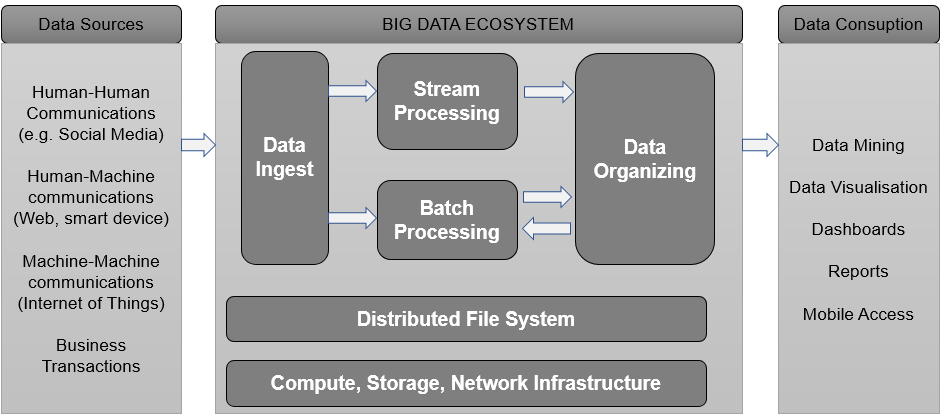
\includegraphics[width=\linewidth]{illustrations/bigdata-architecture}
		 	\caption{Architecture standard du Big Data. Source :  \cite{anil-big-data}}
		 	\label{fig:bigdata-architecture}
		 \end{figure}
		
		Dans un premier temps, les données sont   accueillies   via la couche  \textit{ingest system} par diverses sources de données. Ensuite, les données sont traitées selon deux modes :  \textit{stream processing } et  \textit{batch processing}.  Les résultats de ce traitement peuvent être envoyés vers les bases de données NoSQL (voir la section \ref{sec:nosql}) pour une utilisation ultérieure, ou bien être utilisés  comme entrées pour d'autres applications.  Une solution Big Data comprend typiquement  ces  couches logiques. Chaque  couche peut être représentée par une ou plusieurs technologies disponibles. Reprenons chaque couche logique:
		
		
		%\begin{description}
			\paragraph{Data sources layer} Le choix des sources de donnés pour une application donnée dépend des objectifs qui dirigent l'analyse en question. Les sources avec leurs différents aspects sont détaillées dans la section \ref{variete-data}.
		\paragraph{Data Ingest layer} Cette couche permet de récupérer les données depuis les différentes sources de données. Les données sont accueillies à travers des points d'entrées multiples. Ces points  sont capables de recevoir  ces données ayant une vélocité variable ainsi qu'une quantité aussi variable.  Après avoir traversé  la couche \textit{Data Ingest}, les données sont envoyées au \textit{batch processing system}, au \textit{stream processing system}, ou bien à un système de stockage particulier.
		\paragraph{Batch processing layer} Les données reçues sur cette couche sont celles en provenance du \textit{Data Ingest} ou bien d'une des bases de données NoSQL. Ces données sont ensuite traitées, par exemple, en utilisant les techniques de la programmation parallèle en vue de fournir les résultats souhaités dans un temps raisonnable. La présente couche doit avoir connaissance des sources de données, des types de données, des algorithmes qui vont travailler sur ces données et enfin des résultats souhaités. Les résultats des traitements peuvent être utilisés par une des applications ou bien être sauvegardés dans une des bases de données adaptées.\par
		\paragraph{Stream Processing layer} Cette couche approvisionne les données directement d'une des entrées du \textit{Data Ingest layer}; c'est ce qui différencie cette couche de la couche Batch processing layer. En revanche, \textit{Stream Processing} est similaire à la couche   \textit{Batch processing} en matière  des techniques de la programmation parallèle utilisées ainsi que la nécessité d'avoir les détails sur les sources des données, les types de données et les résultats souhaités.\par
		\paragraph{Data organizing layer} Le rôle de cette couche est d'organiser les données en provenance de la  couche  \textit{Stream Processing} et de la couche \textit{Batch processing}. Cette couche est représentée par les bases de données NoSQL. 
		 %afin de faciliter l'accès à ces dernières. Ce sont les  données obtenues  de la part .
		\paragraph{Infrastructure layer} Cette composante est responsable de la gestion des ressources de stockage, des ressources du calcul et de la gestion de la communication. Les fonctionnalités de cette couche sont typiquement fournies à travers le cloud computing.
		\paragraph{Distributed File System layer} Cette couche permet de stocker une grande quantité de données, de sorte que ces données soient rapidement et facilement accessibles à toutes les couches qui forment un système  Big Data. C'est ce qu'assure, par exemple, Hadoop Distributed File System (HDFS).
		\paragraph{Data consumption layer} Cette dernière couche utilise les résultats obtenus par les couches de l'analyse. Les résultats fournis peuvent être exprimés avec des rapports, des tableaux d'indicateurs, des visualisations, un moteur de recommandation ou tout autre format.
	\subsection{Les bases de données NoSQL (Not Only SQL) } \label{sec:nosql}
	\paragraph{Introduction } ~
	
    Au cours de ces dernières années, on constate une révolution dans le stockage de données non structurées ayant une taille importante.  De plus,  les objets à sauvegarder sont complexes; ils sont issus de sources hétérogènes.  Cette complexité a mis en question les performances des bases de données relationnelles. 
	
	Le terme NoSQL est apparu pour la première fois en $ 1998 $. Carlo Strozzi \cite{CarloStrozziNosql} a parlé des bases de données relationnelles qui n'utilisent pas le SQL comme langage d'interrogation des tables. Des années plus tard, des solutions  open source basées sur ce concept ont vu le jour. 
	
	Les bases de données relationnelles sont conçues pour gérer les données structurées et sont optimisées pour offrir la précision et la cohérence de données. De plus, elles sont utilisées par de nombreuses entreprises pour plusieurs raisons comme   la facilité d'utilisation, la disponibilité de plusieurs produits et développeurs, etc. Ces dernières années, avec l'augmentation exponentielle de la quantité de données générées par certaines entreprises, ces dernières ont constaté l'insuffisance des Systèmes de Gestion de Bases de Données Relationnelles (SGBDR) pour répondre à leurs besoins.
	
    %	\paragraph{ Les besoins auxquels répondent NoSQL}  ~
	Les bases de données NoSQL sont conçues pour gérer des  volumes de données importants. Le flux ainsi que la structure de  ces données sont imprévisibles. C'est pourquoi les bases de données relationnelles ne sont pas convenables. L'idée  des bases de données NoSQL, c'est d'abord assurer la capacité de stocker des données à grande échelle dont la  quantité  évolue rapidement, voire exponentiellement.  En deuxième lieu, les données stockées  doivent être interrogées  avec efficacité. Les données stockées dans  les bases de données NoSQL n'obéissent pas à un modèle prédéfini comme c'est le cas pour les bases de données relationnelles. Cette flexibilité est une des caractéristiques des bases de données NoSQL.
	\paragraph{Types de base de données NoSQL} \label{sec:nosql-database}  ~
	
	Il existe quatre catégories distinctes de bases de données NoSQL. Chaque catégorie répond  à des besoins particuliers. On distingue les bases de données clé-valeur, document, graphe et colonne.
	\subparagraph {Clé-valeur} Une base de données de type clé-valeur repose sur le paradigme clé-valeur; chaque donnée, que ce soit un nombre, du texte ou tout autre type est associé à une clé unique. Cette clé est le seul moyen d'accéder aux données stockées.
	Dans les bases de données NoSQL de type clé-valeur, les enregistrements  n'adhèrent pas à une structure prédéfinie. Par exemple, on peut avoir le premier enregistrement de type entier et le deuxième enregistrement de type texte. Cela assure une forte évolutivité grâce à l'absence d'une structure ou de typage. La Figure \ref{fig:key-value-nosql} montre un exemple de données stockées sous forme de paires clé-valeur.
	\begin{figure}[h]
		\captionsetup{justification=centering}
		\centering
		\resizebox{.4\textwidth}{!}{
			% Graphic for TeX using PGF
% Title: /home/hayat/RipeAtlasTraceroutesAnalysis/2019/Rapport_Mai/illustrations/key-value-nosql.dia
% Creator: Dia v0.97+git
% CreationDate: Tue May  7 11:51:50 2019
% For: hayat
% \usepackage{tikz}
% The following commands are not supported in PSTricks at present
% We define them conditionally, so when they are implemented,
% this pgf file will use them.
\ifx\du\undefined
  \newlength{\du}
\fi
\setlength{\du}{15\unitlength}
\begin{tikzpicture}[even odd rule]
\pgftransformxscale{1.000000}
\pgftransformyscale{-1.000000}
\definecolor{dialinecolor}{rgb}{0.000000, 0.000000, 0.000000}
\pgfsetstrokecolor{dialinecolor}
\pgfsetstrokeopacity{1.000000}
\definecolor{diafillcolor}{rgb}{1.000000, 1.000000, 1.000000}
\pgfsetfillcolor{diafillcolor}
\pgfsetfillopacity{1.000000}
\pgfsetlinewidth{0.000000\du}
\pgfsetdash{}{0pt}
\pgfsetmiterjoin
\definecolor{diafillcolor}{rgb}{0.960784, 0.960784, 0.960784}
\pgfsetfillcolor{diafillcolor}
\pgfsetfillopacity{1.000000}
\pgfpathellipse{\pgfpoint{7.950991\du}{7.987995\du}}{\pgfpoint{1.899011\du}{0\du}}{\pgfpoint{0\du}{1.012005\du}}
\pgfusepath{fill}
\definecolor{dialinecolor}{rgb}{0.000000, 0.000000, 0.000000}
\pgfsetstrokecolor{dialinecolor}
\pgfsetstrokeopacity{1.000000}
\pgfpathellipse{\pgfpoint{7.950991\du}{7.987995\du}}{\pgfpoint{1.899011\du}{0\du}}{\pgfpoint{0\du}{1.012005\du}}
\pgfusepath{stroke}
% setfont left to latex
\definecolor{dialinecolor}{rgb}{0.000000, 0.000000, 0.000000}
\pgfsetstrokecolor{dialinecolor}
\pgfsetstrokeopacity{1.000000}
\definecolor{diafillcolor}{rgb}{0.000000, 0.000000, 0.000000}
\pgfsetfillcolor{diafillcolor}
\pgfsetfillopacity{1.000000}
\node[anchor=base,inner sep=0pt, outer sep=0pt,color=dialinecolor] at (7.950991\du,8.182995\du){001};
\pgfsetlinewidth{0.000000\du}
\pgfsetdash{}{0pt}
\pgfsetmiterjoin
\definecolor{diafillcolor}{rgb}{0.960784, 0.960784, 0.960784}
\pgfsetfillcolor{diafillcolor}
\pgfsetfillopacity{1.000000}
\pgfpathellipse{\pgfpoint{8.024011\du}{10.672005\du}}{\pgfpoint{1.899011\du}{0\du}}{\pgfpoint{0\du}{1.012005\du}}
\pgfusepath{fill}
\definecolor{dialinecolor}{rgb}{0.000000, 0.000000, 0.000000}
\pgfsetstrokecolor{dialinecolor}
\pgfsetstrokeopacity{1.000000}
\pgfpathellipse{\pgfpoint{8.024011\du}{10.672005\du}}{\pgfpoint{1.899011\du}{0\du}}{\pgfpoint{0\du}{1.012005\du}}
\pgfusepath{stroke}
% setfont left to latex
\definecolor{dialinecolor}{rgb}{0.000000, 0.000000, 0.000000}
\pgfsetstrokecolor{dialinecolor}
\pgfsetstrokeopacity{1.000000}
\definecolor{diafillcolor}{rgb}{0.000000, 0.000000, 0.000000}
\pgfsetfillcolor{diafillcolor}
\pgfsetfillopacity{1.000000}
\node[anchor=base,inner sep=0pt, outer sep=0pt,color=dialinecolor] at (8.024011\du,10.867005\du){029};
\pgfsetlinewidth{0.000000\du}
\pgfsetdash{}{0pt}
\pgfsetmiterjoin
\definecolor{diafillcolor}{rgb}{0.960784, 0.960784, 0.960784}
\pgfsetfillcolor{diafillcolor}
\pgfsetfillopacity{1.000000}
\pgfpathellipse{\pgfpoint{7.949011\du}{13.432005\du}}{\pgfpoint{1.899011\du}{0\du}}{\pgfpoint{0\du}{1.012005\du}}
\pgfusepath{fill}
\definecolor{dialinecolor}{rgb}{0.000000, 0.000000, 0.000000}
\pgfsetstrokecolor{dialinecolor}
\pgfsetstrokeopacity{1.000000}
\pgfpathellipse{\pgfpoint{7.949011\du}{13.432005\du}}{\pgfpoint{1.899011\du}{0\du}}{\pgfpoint{0\du}{1.012005\du}}
\pgfusepath{stroke}
% setfont left to latex
\definecolor{dialinecolor}{rgb}{0.000000, 0.000000, 0.000000}
\pgfsetstrokecolor{dialinecolor}
\pgfsetstrokeopacity{1.000000}
\definecolor{diafillcolor}{rgb}{0.000000, 0.000000, 0.000000}
\pgfsetfillcolor{diafillcolor}
\pgfsetfillopacity{1.000000}
\node[anchor=base,inner sep=0pt, outer sep=0pt,color=dialinecolor] at (7.949011\du,13.627005\du){03};
\pgfsetlinewidth{0.000000\du}
\pgfsetdash{}{0pt}
\pgfsetmiterjoin
{\pgfsetcornersarced{\pgfpoint{0.000000\du}{0.000000\du}}\definecolor{diafillcolor}{rgb}{0.960784, 0.960784, 0.862745}
\pgfsetfillcolor{diafillcolor}
\pgfsetfillopacity{1.000000}
\fill (11.525300\du,7.050000\du)--(11.525300\du,8.850000\du)--(21.369346\du,8.850000\du)--(21.369346\du,7.050000\du)--cycle;
}{\pgfsetcornersarced{\pgfpoint{0.000000\du}{0.000000\du}}\definecolor{dialinecolor}{rgb}{0.000000, 0.000000, 0.000000}
\pgfsetstrokecolor{dialinecolor}
\pgfsetstrokeopacity{1.000000}
\draw (11.525300\du,7.050000\du)--(11.525300\du,8.850000\du)--(21.369346\du,8.850000\du)--(21.369346\du,7.050000\du)--cycle;
}% setfont left to latex
\definecolor{dialinecolor}{rgb}{0.000000, 0.000000, 0.000000}
\pgfsetstrokecolor{dialinecolor}
\pgfsetstrokeopacity{1.000000}
\definecolor{diafillcolor}{rgb}{0.000000, 0.000000, 0.000000}
\pgfsetfillcolor{diafillcolor}
\pgfsetfillopacity{1.000000}
\node[anchor=base,inner sep=0pt, outer sep=0pt,color=dialinecolor] at (16.447323\du,8.145000\du){\{"name" : "Toto", age : 12\}};
\pgfsetlinewidth{0.000000\du}
\pgfsetdash{}{0pt}
\pgfsetmiterjoin
{\pgfsetcornersarced{\pgfpoint{0.000000\du}{0.000000\du}}\definecolor{diafillcolor}{rgb}{0.960784, 0.960784, 0.862745}
\pgfsetfillcolor{diafillcolor}
\pgfsetfillopacity{1.000000}
\fill (11.525300\du,9.760000\du)--(11.525300\du,11.560000\du)--(21.479549\du,11.560000\du)--(21.479549\du,9.760000\du)--cycle;
}{\pgfsetcornersarced{\pgfpoint{0.000000\du}{0.000000\du}}\definecolor{dialinecolor}{rgb}{0.000000, 0.000000, 0.000000}
\pgfsetstrokecolor{dialinecolor}
\pgfsetstrokeopacity{1.000000}
\draw (11.525300\du,9.760000\du)--(11.525300\du,11.560000\du)--(21.479549\du,11.560000\du)--(21.479549\du,9.760000\du)--cycle;
}% setfont left to latex
\definecolor{dialinecolor}{rgb}{0.000000, 0.000000, 0.000000}
\pgfsetstrokecolor{dialinecolor}
\pgfsetstrokeopacity{1.000000}
\definecolor{diafillcolor}{rgb}{0.000000, 0.000000, 0.000000}
\pgfsetfillcolor{diafillcolor}
\pgfsetfillopacity{1.000000}
\node[anchor=base,inner sep=0pt, outer sep=0pt,color=dialinecolor] at (16.502425\du,10.855000\du){"Hello World"};
\pgfsetlinewidth{0.000000\du}
\pgfsetdash{}{0pt}
\pgfsetmiterjoin
{\pgfsetcornersarced{\pgfpoint{0.000000\du}{0.000000\du}}\definecolor{diafillcolor}{rgb}{0.960784, 0.960784, 0.862745}
\pgfsetfillcolor{diafillcolor}
\pgfsetfillopacity{1.000000}
\fill (11.503500\du,12.510000\du)--(11.503500\du,14.310000\du)--(21.501313\du,14.310000\du)--(21.501313\du,12.510000\du)--cycle;
}{\pgfsetcornersarced{\pgfpoint{0.000000\du}{0.000000\du}}\definecolor{dialinecolor}{rgb}{0.000000, 0.000000, 0.000000}
\pgfsetstrokecolor{dialinecolor}
\pgfsetstrokeopacity{1.000000}
\draw (11.503500\du,12.510000\du)--(11.503500\du,14.310000\du)--(21.501313\du,14.310000\du)--(21.501313\du,12.510000\du)--cycle;
}% setfont left to latex
\definecolor{dialinecolor}{rgb}{0.000000, 0.000000, 0.000000}
\pgfsetstrokecolor{dialinecolor}
\pgfsetstrokeopacity{1.000000}
\definecolor{diafillcolor}{rgb}{0.000000, 0.000000, 0.000000}
\pgfsetfillcolor{diafillcolor}
\pgfsetfillopacity{1.000000}
\node[anchor=base,inner sep=0pt, outer sep=0pt,color=dialinecolor] at (16.502406\du,13.605000\du){1557177896 };
\pgfsetlinewidth{0.100000\du}
\pgfsetdash{}{0pt}
\pgfsetbuttcap
{
\definecolor{diafillcolor}{rgb}{0.000000, 0.000000, 0.000000}
\pgfsetfillcolor{diafillcolor}
\pgfsetfillopacity{1.000000}
% was here!!!
\pgfsetarrowsend{to}
\definecolor{dialinecolor}{rgb}{0.000000, 0.000000, 0.000000}
\pgfsetstrokecolor{dialinecolor}
\pgfsetstrokeopacity{1.000000}
\draw (9.850000\du,7.988000\du)--(11.525300\du,7.950000\du);
}
\pgfsetlinewidth{0.100000\du}
\pgfsetdash{}{0pt}
\pgfsetbuttcap
{
\definecolor{diafillcolor}{rgb}{0.000000, 0.000000, 0.000000}
\pgfsetfillcolor{diafillcolor}
\pgfsetfillopacity{1.000000}
% was here!!!
\pgfsetarrowsend{to}
\definecolor{dialinecolor}{rgb}{0.000000, 0.000000, 0.000000}
\pgfsetstrokecolor{dialinecolor}
\pgfsetstrokeopacity{1.000000}
\draw (9.923020\du,10.672000\du)--(11.525300\du,10.660000\du);
}
\pgfsetlinewidth{0.100000\du}
\pgfsetdash{}{0pt}
\pgfsetbuttcap
{
\definecolor{diafillcolor}{rgb}{0.000000, 0.000000, 0.000000}
\pgfsetfillcolor{diafillcolor}
\pgfsetfillopacity{1.000000}
% was here!!!
\pgfsetarrowsend{to}
\definecolor{dialinecolor}{rgb}{0.000000, 0.000000, 0.000000}
\pgfsetstrokecolor{dialinecolor}
\pgfsetstrokeopacity{1.000000}
\draw (9.848020\du,13.432000\du)--(11.503500\du,13.410000\du);
}
\end{tikzpicture}

	    }
		\caption{Illustration d'une base de données NoSQL de type clé-valeur}
		\label{fig:key-value-nosql}
	\end{figure}

	\subparagraph{Graphe} Dans une base de données de type graphe, les données stockées sont les n\oe{}uds, les liens et les propriétés sur les n\oe{}uds et sur les liens. Un exemple  de base de données NoSQL de type graphe est le réseau social; chaque entité représente une personne et les relations entre ces personnes peuvent prendre plusieurs formes. Un autre exemple de données stockées  dans une base de données orientée graphe est donné dans la Figure  	\ref{fig:graphe-nosql}. Avec cette représentation, par exemple, on peut chercher les membres du groupe \textit{Chess}.  
\begin{figure}[h]
	\centering
	%	\resizebox{\textwidth}{!}{
	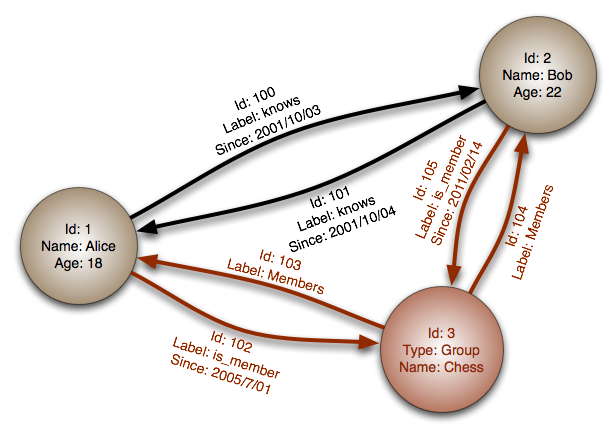
\includegraphics[width=.9\linewidth]{illustrations/GraphDatabase_PropertyGraph.png}		
	%   }
	\caption{Illustration d'une base de données NoSQL de type graphe. Source : \url{https://en.wikipedia.org/wiki/Graph_database}, consultée le $10/05/2019$}
	\label{fig:graphe-nosql}
\end{figure}
		\subparagraph{Document} Une base de données NoSQL de type document permet de stocker les données en reposant sur le paradigme clé-valeur. Toutefois, les valeur stockées sont complexes, il s'agit de documents de type JSON, XML, etc. L'accès aux données d'un enregistrement peut se faire de manière hiérarchique. La possibilité de stocker des objets complexes et hétérogènes  est un des points forts des bases de données NoSQL de type  document. Un exemple est fourni dans la Figure \ref{fig:document-nosql}. Une des différences majeures entre les bases de données clé-valeur et celles de type document c'est que pour les premières, l'indexation est au niveau  des clés seulement, tandis que pour les deuxièmes, l'indexation est au niveau clé et valeur. En pratique, pour les bases de données clé-valeur, les données sont récupérées en se basant sur la clé et pour les autres, la récupération d'un enregistrement peut être basée sur la clé et sur la valeur étant donné que la valeur est semi-structuré (valeur de type JSON, XML, etc.)
		\begin{figure}[h]
			\centering
				\resizebox{\textwidth}{!}{
			% Graphic for TeX using PGF
% Title: /home/hayat/RipeAtlasTraceroutesAnalysis/2019/Rapport_Mai/illustrations/document-nosql.dia
% Creator: Dia v0.97+git
% CreationDate: Tue May  7 11:56:16 2019
% For: hayat
% \usepackage{tikz}
% The following commands are not supported in PSTricks at present
% We define them conditionally, so when they are implemented,
% this pgf file will use them.
\ifx\du\undefined
  \newlength{\du}
\fi
\setlength{\du}{15\unitlength}
\begin{tikzpicture}[even odd rule]
\pgftransformxscale{1.000000}
\pgftransformyscale{-1.000000}
\definecolor{dialinecolor}{rgb}{0.000000, 0.000000, 0.000000}
\pgfsetstrokecolor{dialinecolor}
\pgfsetstrokeopacity{1.000000}
\definecolor{diafillcolor}{rgb}{1.000000, 1.000000, 1.000000}
\pgfsetfillcolor{diafillcolor}
\pgfsetfillopacity{1.000000}
\pgfsetlinewidth{0.000000\du}
\pgfsetdash{}{0pt}
\pgfsetmiterjoin
\definecolor{diafillcolor}{rgb}{0.960784, 0.960784, 0.960784}
\pgfsetfillcolor{diafillcolor}
\pgfsetfillopacity{1.000000}
\pgfpathellipse{\pgfpoint{7.395991\du}{3.752005\du}}{\pgfpoint{1.899011\du}{0\du}}{\pgfpoint{0\du}{1.012005\du}}
\pgfusepath{fill}
\definecolor{dialinecolor}{rgb}{0.000000, 0.000000, 0.000000}
\pgfsetstrokecolor{dialinecolor}
\pgfsetstrokeopacity{1.000000}
\pgfpathellipse{\pgfpoint{7.395991\du}{3.752005\du}}{\pgfpoint{1.899011\du}{0\du}}{\pgfpoint{0\du}{1.012005\du}}
\pgfusepath{stroke}
% setfont left to latex
\definecolor{dialinecolor}{rgb}{0.000000, 0.000000, 0.000000}
\pgfsetstrokecolor{dialinecolor}
\pgfsetstrokeopacity{1.000000}
\definecolor{diafillcolor}{rgb}{0.000000, 0.000000, 0.000000}
\pgfsetfillcolor{diafillcolor}
\pgfsetfillopacity{1.000000}
\node[anchor=base,inner sep=0pt, outer sep=0pt,color=dialinecolor] at (7.395991\du,3.947005\du){ta};
\pgfsetlinewidth{0.000000\du}
\pgfsetdash{}{0pt}
\pgfsetmiterjoin
\definecolor{diafillcolor}{rgb}{0.960784, 0.960784, 0.960784}
\pgfsetfillcolor{diafillcolor}
\pgfsetfillopacity{1.000000}
\pgfpathellipse{\pgfpoint{7.469011\du}{6.436015\du}}{\pgfpoint{1.899011\du}{0\du}}{\pgfpoint{0\du}{1.012005\du}}
\pgfusepath{fill}
\definecolor{dialinecolor}{rgb}{0.000000, 0.000000, 0.000000}
\pgfsetstrokecolor{dialinecolor}
\pgfsetstrokeopacity{1.000000}
\pgfpathellipse{\pgfpoint{7.469011\du}{6.436015\du}}{\pgfpoint{1.899011\du}{0\du}}{\pgfpoint{0\du}{1.012005\du}}
\pgfusepath{stroke}
% setfont left to latex
\definecolor{dialinecolor}{rgb}{0.000000, 0.000000, 0.000000}
\pgfsetstrokecolor{dialinecolor}
\pgfsetstrokeopacity{1.000000}
\definecolor{diafillcolor}{rgb}{0.000000, 0.000000, 0.000000}
\pgfsetfillcolor{diafillcolor}
\pgfsetfillopacity{1.000000}
\node[anchor=base,inner sep=0pt, outer sep=0pt,color=dialinecolor] at (7.469011\du,6.631015\du){tb};
\pgfsetlinewidth{0.000000\du}
\pgfsetdash{}{0pt}
\pgfsetmiterjoin
\definecolor{diafillcolor}{rgb}{0.960784, 0.960784, 0.960784}
\pgfsetfillcolor{diafillcolor}
\pgfsetfillopacity{1.000000}
\pgfpathellipse{\pgfpoint{7.394011\du}{9.196015\du}}{\pgfpoint{1.899011\du}{0\du}}{\pgfpoint{0\du}{1.012005\du}}
\pgfusepath{fill}
\definecolor{dialinecolor}{rgb}{0.000000, 0.000000, 0.000000}
\pgfsetstrokecolor{dialinecolor}
\pgfsetstrokeopacity{1.000000}
\pgfpathellipse{\pgfpoint{7.394011\du}{9.196015\du}}{\pgfpoint{1.899011\du}{0\du}}{\pgfpoint{0\du}{1.012005\du}}
\pgfusepath{stroke}
% setfont left to latex
\definecolor{dialinecolor}{rgb}{0.000000, 0.000000, 0.000000}
\pgfsetstrokecolor{dialinecolor}
\pgfsetstrokeopacity{1.000000}
\definecolor{diafillcolor}{rgb}{0.000000, 0.000000, 0.000000}
\pgfsetfillcolor{diafillcolor}
\pgfsetfillopacity{1.000000}
\node[anchor=base,inner sep=0pt, outer sep=0pt,color=dialinecolor] at (7.394011\du,9.391015\du){tc};
\pgfsetlinewidth{0.000000\du}
\pgfsetdash{}{0pt}
\pgfsetmiterjoin
{\pgfsetcornersarced{\pgfpoint{0.000000\du}{0.000000\du}}\definecolor{diafillcolor}{rgb}{0.960784, 0.960784, 0.862745}
\pgfsetfillcolor{diafillcolor}
\pgfsetfillopacity{1.000000}
\fill (12.651200\du,2.864010\du)--(12.651200\du,4.664010\du)--(49.000000\du,4.664010\du)--(49.000000\du,2.864010\du)--cycle;
}{\pgfsetcornersarced{\pgfpoint{0.000000\du}{0.000000\du}}\definecolor{dialinecolor}{rgb}{0.000000, 0.000000, 0.000000}
\pgfsetstrokecolor{dialinecolor}
\pgfsetstrokeopacity{1.000000}
\draw (12.651200\du,2.864010\du)--(12.651200\du,4.664010\du)--(49.000000\du,4.664010\du)--(49.000000\du,2.864010\du)--cycle;
}% setfont left to latex
\definecolor{dialinecolor}{rgb}{0.000000, 0.000000, 0.000000}
\pgfsetstrokecolor{dialinecolor}
\pgfsetstrokeopacity{1.000000}
\definecolor{diafillcolor}{rgb}{0.000000, 0.000000, 0.000000}
\pgfsetfillcolor{diafillcolor}
\pgfsetfillopacity{1.000000}
\node[anchor=base,inner sep=0pt, outer sep=0pt,color=dialinecolor] at (30.825600\du,3.959010\du){\{"timestamp":1427847501,"type":"traceroute"\}};
\pgfsetlinewidth{0.000000\du}
\pgfsetdash{}{0pt}
\pgfsetmiterjoin
{\pgfsetcornersarced{\pgfpoint{0.000000\du}{0.000000\du}}\definecolor{diafillcolor}{rgb}{0.960784, 0.960784, 0.862745}
\pgfsetfillcolor{diafillcolor}
\pgfsetfillopacity{1.000000}
\fill (12.570000\du,5.574010\du)--(12.570000\du,7.374010\du)--(49.000000\du,7.374010\du)--(49.000000\du,5.574010\du)--cycle;
}{\pgfsetcornersarced{\pgfpoint{0.000000\du}{0.000000\du}}\definecolor{dialinecolor}{rgb}{0.000000, 0.000000, 0.000000}
\pgfsetstrokecolor{dialinecolor}
\pgfsetstrokeopacity{1.000000}
\draw (12.570000\du,5.574010\du)--(12.570000\du,7.374010\du)--(49.000000\du,7.374010\du)--(49.000000\du,5.574010\du)--cycle;
}% setfont left to latex
\definecolor{dialinecolor}{rgb}{0.000000, 0.000000, 0.000000}
\pgfsetstrokecolor{dialinecolor}
\pgfsetstrokeopacity{1.000000}
\definecolor{diafillcolor}{rgb}{0.000000, 0.000000, 0.000000}
\pgfsetfillcolor{diafillcolor}
\pgfsetfillopacity{1.000000}
\node[anchor=base,inner sep=0pt, outer sep=0pt,color=dialinecolor] at (30.785000\du,6.669010\du){\{"af":6,"dst\_addr":"2001:7fd::1","timestamp":1427847501,"type":"traceroute"\}};
\pgfsetlinewidth{0.000000\du}
\pgfsetdash{}{0pt}
\pgfsetmiterjoin
{\pgfsetcornersarced{\pgfpoint{0.000000\du}{0.000000\du}}\definecolor{diafillcolor}{rgb}{0.960784, 0.960784, 0.862745}
\pgfsetfillcolor{diafillcolor}
\pgfsetfillopacity{1.000000}
\fill (12.620000\du,8.324010\du)--(12.620000\du,10.124010\du)--(48.995000\du,10.124010\du)--(48.995000\du,8.324010\du)--cycle;
}{\pgfsetcornersarced{\pgfpoint{0.000000\du}{0.000000\du}}\definecolor{dialinecolor}{rgb}{0.000000, 0.000000, 0.000000}
\pgfsetstrokecolor{dialinecolor}
\pgfsetstrokeopacity{1.000000}
\draw (12.620000\du,8.324010\du)--(12.620000\du,10.124010\du)--(48.995000\du,10.124010\du)--(48.995000\du,8.324010\du)--cycle;
}% setfont left to latex
\definecolor{dialinecolor}{rgb}{0.000000, 0.000000, 0.000000}
\pgfsetstrokecolor{dialinecolor}
\pgfsetstrokeopacity{1.000000}
\definecolor{diafillcolor}{rgb}{0.000000, 0.000000, 0.000000}
\pgfsetfillcolor{diafillcolor}
\pgfsetfillopacity{1.000000}
\node[anchor=base,inner sep=0pt, outer sep=0pt,color=dialinecolor] at (30.807500\du,9.419010\du){\{"af":6, "result":\ensuremath{[}\{"hop":1,"result":\ensuremath{[}\{"from":"2a01:240:fec5::ff","rtt":0.477,"size":88,"ttl":64\}\ensuremath{]}\}\ensuremath{]}\}};
\pgfsetlinewidth{0.100000\du}
\pgfsetdash{}{0pt}
\pgfsetbuttcap
{
\definecolor{diafillcolor}{rgb}{0.000000, 0.000000, 0.000000}
\pgfsetfillcolor{diafillcolor}
\pgfsetfillopacity{1.000000}
% was here!!!
\pgfsetarrowsend{to}
\definecolor{dialinecolor}{rgb}{0.000000, 0.000000, 0.000000}
\pgfsetstrokecolor{dialinecolor}
\pgfsetstrokeopacity{1.000000}
\draw (9.295000\du,3.752010\du)--(12.651200\du,3.764010\du);
}
\pgfsetlinewidth{0.100000\du}
\pgfsetdash{}{0pt}
\pgfsetbuttcap
{
\definecolor{diafillcolor}{rgb}{0.000000, 0.000000, 0.000000}
\pgfsetfillcolor{diafillcolor}
\pgfsetfillopacity{1.000000}
% was here!!!
\pgfsetarrowsend{to}
\definecolor{dialinecolor}{rgb}{0.000000, 0.000000, 0.000000}
\pgfsetstrokecolor{dialinecolor}
\pgfsetstrokeopacity{1.000000}
\draw (9.368020\du,6.436010\du)--(12.570000\du,6.474010\du);
}
\pgfsetlinewidth{0.100000\du}
\pgfsetdash{}{0pt}
\pgfsetbuttcap
{
\definecolor{diafillcolor}{rgb}{0.000000, 0.000000, 0.000000}
\pgfsetfillcolor{diafillcolor}
\pgfsetfillopacity{1.000000}
% was here!!!
\pgfsetarrowsend{to}
\definecolor{dialinecolor}{rgb}{0.000000, 0.000000, 0.000000}
\pgfsetstrokecolor{dialinecolor}
\pgfsetstrokeopacity{1.000000}
\draw (9.293020\du,9.196010\du)--(12.620000\du,9.224010\du);
}
% setfont left to latex
\definecolor{dialinecolor}{rgb}{0.000000, 0.000000, 0.000000}
\pgfsetstrokecolor{dialinecolor}
\pgfsetstrokeopacity{1.000000}
\definecolor{diafillcolor}{rgb}{0.000000, 0.000000, 0.000000}
\pgfsetfillcolor{diafillcolor}
\pgfsetfillopacity{1.000000}
\node[anchor=base west,inner sep=0pt,outer sep=0pt,color=dialinecolor] at (9.850000\du,14.350000\du){};
\end{tikzpicture}

		}
			\caption{Illustration d'une base de données NoSQL de type document}
			\label{fig:document-nosql}
		\end{figure}
		\subparagraph{Colonnes} Dans les bases de données traditionnelles, les données sont stockées sur des lignes. Dans le cas d'une base NoSQL orientée colonne, les données sont stockées par colonne. L'interrogation de ce type de bases travaille sur une colonne particulière sans devoir passer par les autres colonnes comme dans les bases de données relationnelles classiques. Une base de données de type colonne est adaptée pour les requêtes analytiques comme les requêtes d'agrégation (moyennes, maximum, etc). La Figure \ref{fig:comomn-nosql} illustre la différence entre le stockage dans une base de données relationnelle et une base de données orientée colonnes\footnote{Cette illustration  est basée sur une figure disponible sur \url{https://www.illustradata.com/bases-nosql-orientees-colonnes-quest-cest}, consulté le $02/05/2019$.}. 
		Les bases de données NoSQL orientées colonnes sont conçues pour pouvoir ajouter facilement de nouveaux colonnes, jusqu'à des millions de colonnes. De plus, le coût du stockage de \textit{null} vaut $ 0 $.
		
	\begin{figure}[h]
		\centering
		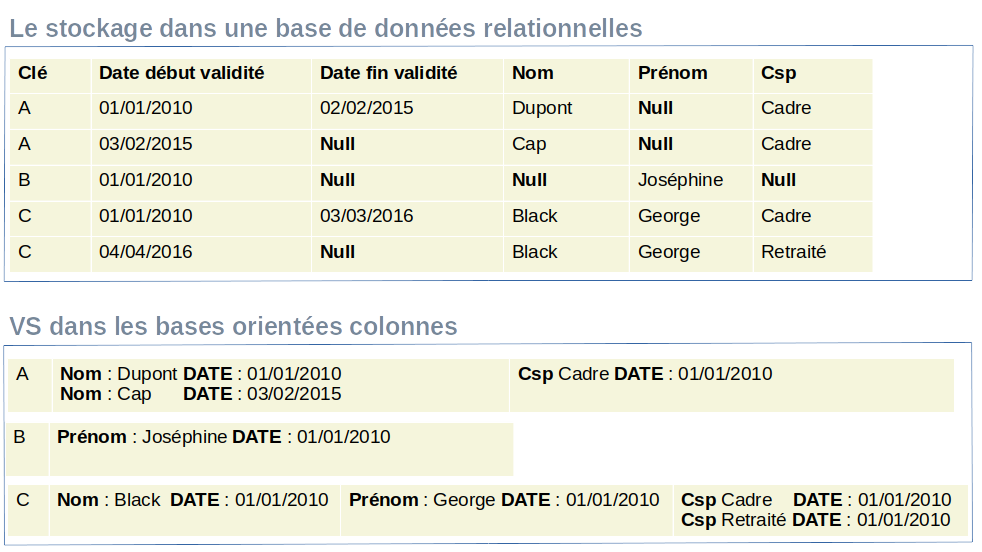
\includegraphics[width=\linewidth]{illustrations/colomn-db-2.png}
		\caption{Illustration d'une base de données NoSQL de type colonne}
		\label{fig:comomn-nosql}
	\end{figure}


Les bases de données NoSQL sont conçues pour répondre à des besoins spécifiques. Elles n'ont pas été créées pour remplacer les bases de données relationnelles. Il existe plusieurs implémentations des quatre types des bases de données NoSQL. Chaque implémentation favorise un ou plusieurs  éléments suivants : la disponibilité des données, la cohérence des données et la tolérance au partitionnement.  C'est ce qu'explique le théorème CAP.	
		\paragraph{Big Data et le théorème  CAP} \label{par:cap-theorem}:
		
		Dans le but d'assurer un traitement rapide de données à grande échelle, ces dernières sont réparties sur un cluster de machines  (appelées aussi  n\oe{}uds). Le théorème CAP annonce que dans le cadre d'un système distribué où le stockage de données est  réparti sur plusieurs machines,
		%(ou n\oe{}uds) (voir \ref{sec:distruted-camput}),  
		une base de données ne peut pas garantir les trois attributs suivants : \textit{Consistency}, \textit{Availability} et \textit{Partition Tolerence}  en même temps. \par
			\textbf{Consistency (ou intégrité)} Chaque donnée a un seul état visible depuis l'extérieur. Par exemple, les différents serveurs hébergeant la base de données voient tous les mêmes données. C'est pourquoi une lecture faite après une écriture doit renvoyer la donnée précédemment écrite. \par
			\textbf{Availability (ou disponibilité)} Une base de données doit toujours fournir une réponse à une requête d'un client.\par
			%En cas d'une panne technique sur un des serveurs qui hébergent  la base de données, il faut s'assurer de desservir  des clients.  Généralement, cela est assuré à travers la réplication des données
			 \textbf{Partition tolerance (ou  tolérance au partitionnement) } Une coupure du réseau entre deux n\oe{}uds ou l'indisponibilité d'un de ces n\oe{}uds ne devrait pas affecter le bon fonctionnement du système. Tout de même,  ce dernier doit répondre à la demande d'un client. 

		
		%conclusion
		Les trois attributs du théorème CAP s'opposent entre eux. On distingue les trois scénarios possibles:
		
		\begin{itemize}
			\item [--] Le couple \textbf{CA} : les SGBDR adoptent les deux attributs C et A, qui sont une forte cohérence et disponibilité. Cependant, l'attribut partitionnement réseau n'est pas toujours pris en compte.
			\item [--] Le couple \textbf{CP} : les implémentations du C et du P assurent la tolérance aux pannes en distribuant les données sur plusieurs serveurs. Malgré cette réplication, ces implémentations assurent la cohérence des données même en présence de mises à jour concurrentielles.
			\item [--] Le couple \textbf{AP} : les implémentations du A et du  P assurent un temps de réponse rapide et une réplication de données. Cependant, les mises à jour étant asynchrones, la garantie que la version d'une donnée soit bonne, ne peut pas être assurée.
			
		\end{itemize}
		
		La Figure \ref{fig:cap} présente des implémentations des différents types de bases de données NoSQL pour chaque couple CA, CP et AP.
		
		\begin{figure}[h]
			\centering
			\captionsetup{justification=centering}
			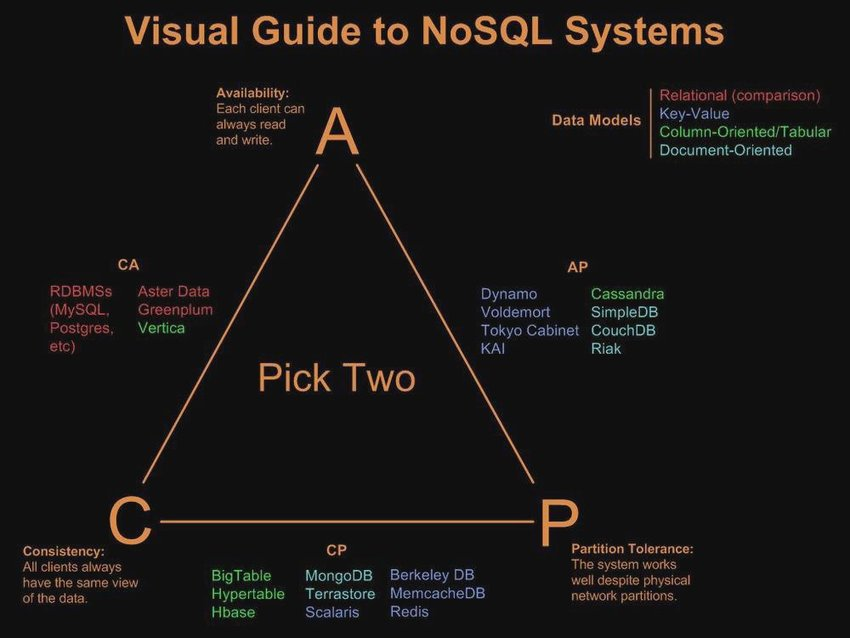
\includegraphics[width=1\linewidth]{illustrations/cap}
			\caption{Bases de données NoSQL suivant le théorème de CAP }
			\label{fig:cap}
			\source{\url{https://www.researchgate.net/figure/CAP-theorem-concept-5-II-WHY-YOU-NEED-NOSQL-The-first-reason-to-use-NoSQL-is-because_fig2_323309389}, consultée le $05/08/2018$.}
		\end{figure}
		
		
		
		Le choix d'une base de données relationnelle ou NoSQL dépend des besoins des entreprises. En terme de tendances, la Figure \ref{fig:ranking-db} reprend un classement des SGBDs au $1$ août $ 2018 $. La suite de la liste ainsi que  la méthode qui dirige ce classement sont    disponibles sur le site  Web \textit{DB-Engines Ranking}\footnote{URL : \url{https://db-engines.com/},  consulté le $01/08/2018$.}. Parmi les critères du classement, on trouve le nombre de références du SGBD sur les sites Internet. 
		
		%Ce nombre de référence est quantifiable à partir du  nombre lui-même de résultats obtenus des différents moteurs de recherche comme Google, Bing, etc. 
		
		\begin{figure}[h]
			\centering
			\captionsetup{justification=centering}
			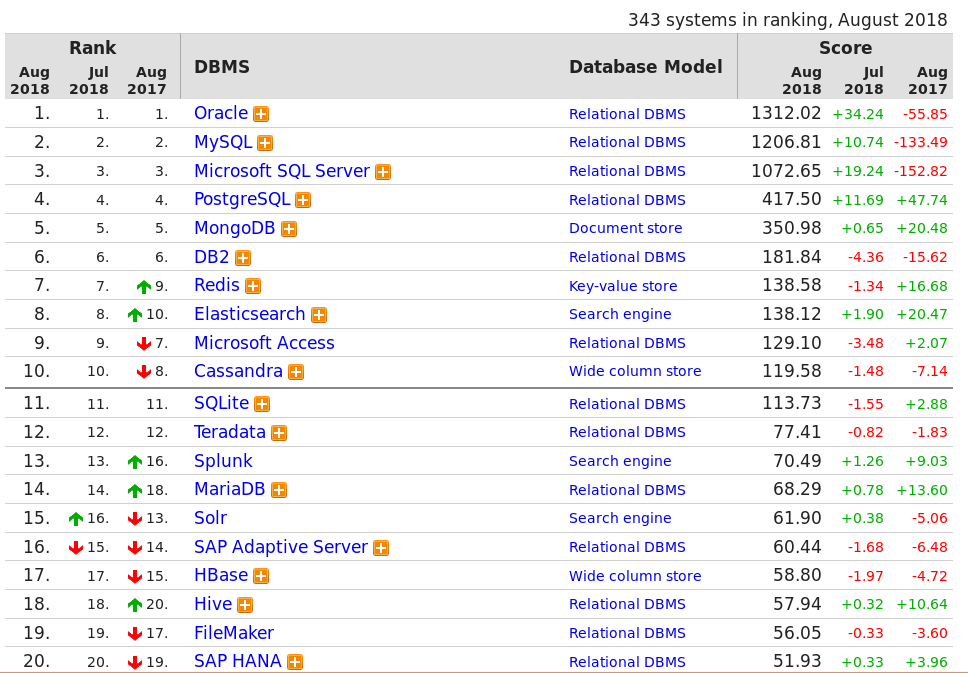
\includegraphics[width=1\linewidth]{illustrations/ranking-db}
			\caption{Un classement des SGBDs sur \textit{DB-Engines Ranking} du $1$ août $2018$ }
			\label{fig:ranking-db}
			\source{\url{https://db-engines.com/en/ranking}, consultée le $01/08/2018$.}
		\end{figure}
		
		\subsection{Extraction, Transformation, Loading (ETL)} \label{sec:etl}
		Dans une même organisation, il est possible d'avoir plusieurs sources de données~: des bases de données relationnelles, des bases de données NoSQL, des fichiers de données de type Excel, etc. 
		Dans le cas où une analyse de données devrait impliquer des données en provenance de  sources  de données hétérogènes, il est nécessaire de faire appel aux opérations ETL :
		
		\textbf{Extraction} :  la diversité des sources de données implique des formats de données différents. Généralement, ce sont des données en provenance des bases de données relationnelles, des fichiers plats, des bases de données non relationnelles,  etc. Le but de la phase d'extraction est de convertir les données en un seul format approprié à l'étape de la transformation. Cette phase  vérifie si les données respectent  une structure attendue. Si ce n'est pas le cas, les données peuvent être totalement ou partiellement rejetées.
		
		\textbf{Transformation} : cette étape  s'applique  sur les données extraites. Elle comprend  une série de règles ou de fonctions. Ces derniers sont appliqués sur les données avant de les envoyer vers la cible. Certaines sources de données nécessitent  peu de transformations, voire aucune. Dans d'autres cas, un ou plusieurs  types de transformation sont  nécessaires. Quelques exemples de transformations  sont    listées ci-dessous :
		\begin{itemize}
			\item sélection d'un nombre  de colonnes à charger parmi plusieurs colonnes;
			\item adaptation des codes. Par exemple,  quand le système de stockage source utilise 1 pour dénoter un homme et l'entrepôt de données cible  utilise "H"; 
			\item conversion des devises, c'est le cas par exemple où les salaires sont exprimés en une devise différente de l'euro;
			\item élimination des doublons.
		\end{itemize}
		
		\textbf{Loading} : l'objectif de cette étape est de charger les données transformées vers l'entrepôt de données. Le chargement des données dépend des besoins de l'organisation. Dans certains cas, on prévoit le remplacement des informations existantes par des informations cumulatives plus récentes. Dans d'autres cas, les nouvelles informations sont ajoutées dans la suite de celles existantes. 
		
		En ce qui concerne la fréquence  des opérations ETL, elles peuvent être planifiées de manière horaire, quotidienne, hebdomadaire, mensuelle ou autre.
		
		 %ETL est un système de chargement de données depuis les différentes sources de données jusqu'à l'entrepôt de données. Ce système  s'occupe de faire passer les données par un ensemble de traitements pour les nettoyer,  les contextualiser et enfin les charger. Les tâches ETL prennent énormément du temps dans un projet d'analyse de données. Il est important d'assurer  la qualité de données et d'éviter les fausses données ou les données inutiles. 
		 
		
		
		
		\subsection{Schema on Write et Schema on Read} \label{sec:schema-read-write}
		
		Lors du chargement des données depuis leurs sources de stockage, on distingue deux approches : \textit{ Schema on Write} et \textit{Schema on Read}.
		% L'approche \textit{Schema on Read } est celle utilisée par l'outil Amazon Athena présenté dans la section \ref{par:allservices}.
		
		Dans la première, il faut définir les colonnes, le format de données, les types, etc. La lecture des données est rapide et moins coûteuse étant donné l'effort entrepris pour définir la structure. C'est le cas des bases de données relationnelles.
		
		Dans la deuxième, les données sont chargées telles qu'elles sont, sans transformations ou changements. L'interprétation de ces données se fait lors de la lecture, et cela dépend des besoins pour lesquels les données sont analysées. Ainsi, les mêmes données peuvent être lues de différentes manières. Par exemple, l'action  de lire les données  d'une colonne, qu'elles soient de type entier ou bien chaîne de caractère d'un fichier CSV est la même, c'est le type de la donnée qui diffère. C'est l'approche utilisée par Amazon Athena (voir la section \ref{aws:athena}). 
		
\paragraph{Exemple illustratif}~

 Afin de montrer la différence entre les deux approches, nous comparons Apache Spark (présenté en détail dans la section \ref{apache-spark}) avec une base de données relationnelle (SQL Server).   Les étapes suivantes concernent  SQL Server:
%\begin{tcolorbox}{SQL RDBMS : exemple de SQL Server}
\begin{enumerate}
	\item Créer la table Traceroutes :
\begin{lstlisting}[language = sql, basicstyle=\small]
CREATE TABLE Traceroutes(
	id INT,
	dst_name VARCHAR(30),
	...
)
\end{lstlisting}
		
	\item  Charger les données depuis le fichier \textit{traceroute-2019-04-08T0000.json} vers la table Traceroutes, chaque ligne du fichier doit correspondre à la  structure  créée à l'étape $ 1 $:
\begin{lstlisting}[language = sql, basicstyle=\small]
BULK INSERT  Traceroutes
FROM 'c:\traceroutes\traceroute-2019-04-08T0000.csv'
WITH ROWTERMINATOR = '\n'
\end{lstlisting}
	
	\item Interroger les données : à l'issue de l'étape $2$,  les données sont chargées et prêtes à l'interrogation: 
\begin{lstlisting}[language = sql, basicstyle=\small]
SELECT dst_name FROM  Traceroutes
\end{lstlisting}
	\end{enumerate}

Pour les bases de données relationnelles, qui adoptent l'approche \textit{Schema on Write}, on ne peut pas ajouter des données avant de créer le schéma dirigeant ces dernières. De plus, la création du schéma nécessite la compréhension  exhaustive des données. 
Car en cas d'un changement du contenu du fichier de données, en terme de structure, la table créée doit être supprimée, mise à jour, ensuite il faut recharger à nouveau les données. L'implication de la mise à jour du schéma peut être coûteuse en terme de temps  dans le cas  d'un  volume de donnée  important, de l'ordre de plusieurs centaines de téraoctets. Dans certains cas, une mise à jour des relations avec d'autres tables est requise.

En ce qui concerne l'approche \textit{Schema on Read}, nous prenons l'exemple d'Apache Spark présenté en détail dans la section \ref{apache-spark}. En utilisant cette technologie, on crée un schéma selon les besoins de l'analyse de ces données.
% et non pas pour que la structure des données soit exactement celle à créer, sauf si cela fait partie des besoins. 
%Par exemple, on peut créer une table dont les colonnes correspondent  seulement à la moitié des colonnes possibles. Un autre exemple concerne l'utilisation  des conditions; on crée une table et durant le chargement des données, on ne charge que celles vérifiant une condition donnée. Pour AWS Athena et les autres technologies qui se basent sur  cette approche, les données sont chargées au moment de l'utilisation et avec plus de flexibilité.
Pour illustrer cette approche, l'annexe \ref{exemple-traceroute} présente une réponse d'une requête traceroute. Pour les besoins de l'outil de détection (voir le chapitre \ref{chap:algorith-detection}), plusieurs attributs ne sont pas pertinents. Ainsi, il est inutile de les charger lors de l'analyse.   En Spark, les données sont lues en associant les attributs d'une classe aux attributs de la réponse traceroute; c'est la classe Traceroute décrite dans le Listing \ref{lst:case-class-Traceroute}. En résultat, seules les données utiles qui sont chargées en mémoire pour qu'elles soient traitées.

La meilleure approche dépend des besoins de l'analyse. La première approche est meilleure en performances, en revanche, la deuxième est tolérante aux erreurs  humaines.

		\subsection{L'informatique distribuée et l'analyse de données massives} \label{sec:distruted-camput}
		Il existe deux stratégies pour appliquer des traitements sur un grand ensemble de données: 
		
		
		\begin{itemize}
			\item[--] Par distribution des traitements (\textit{scaling} des traitements)~: les traitements sont distribués sur un nombre de n\oe{}uds important. De ce fait, les données sont amenées jusqu'à ces n\oe{}uds.
			
			\item[--] Par distribution des données (\textit{scaling} des données)~: les données sont distribuées sur un nombre important de n\oe{}uds. Par ailleurs cela permet  de stocker un maximum de données. Il s'agit d'amener les traitements aux machines sur lesquelles les données sont stockées. Du fait que le stockage de données est réparti sur plusieurs machines, il est possible de traiter des données très volumineuses en un temps optimal. La première mise en \oe{}uvre de cette approche est le schéma MapReduce (voir la section  \ref{mapreducesection}). 
		\end{itemize}
\subsection{MapReduce} \label{mapreducesection}
%https://softwareengineering.stackexchange.com/questions/220605/why-big-data-needs-to-be-functional

MapReduce est un modèle de programmation proposé par Google. Il est conçu pour   le traitement distribué de grands ensembles de données   sur un cluster de machines. Un programme MapReduce est composé de deux phases principales   \textit{Map} et  \textit{Reduce}.

MapReduce divise le travail en petites parties, chacune pouvant être effectuée en parallèle sur le cluster de machines. Autrement dit, le  problème est divisé en un grand nombre de problèmes plus petits, chaque petit problème est traité pour donner des résultats individuelles. Ces résultats sont ensuite traités pour donner un résultat final. 
%Hadoop MapReduce est évolutif et peut également être utilisé sur de nombreux ordinateurs. 
%\begin{tcolorbox}
%	\textit{ MapReduce est un patron d'architecture de développement informatique, inventé par Google, dans lequel sont effectués des %calculs parallèles, et souvent distribués, de données potentiellement très volumineuses, typiquement supérieures en taille à 1 %téraoctet} \footnote{Source : \url{https://fr.wikipedia.org/wiki/MapReduce}, consultée le $20/12/2018$.}. 
%\end{tcolorbox}
La Figure 	\ref{fig:2-figure1-1-map-reduce-workflow} représente une vue d'ensemble du modèle de programmation MapReduce. 

\begin{figure}[h]
	\centering
	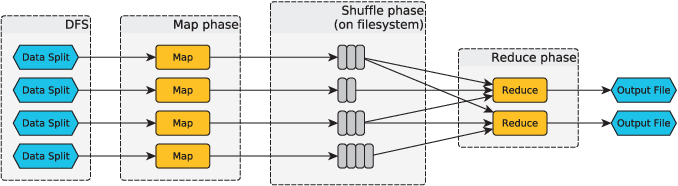
\includegraphics[width=\linewidth]{illustrations/2-Figure1-1-map-reduce-workflow}
	\caption{Vue d'ensemble du modèle MapReduce. Source : \cite{6427487}}
	\label{fig:2-figure1-1-map-reduce-workflow}
\end{figure}


Le modèle de données de base dans MapReduce  est la paire clé/valeur. Pendant la phase de \textit{Map}, la fonction  associée  au Map est exécutée sur chaque paire clé/valeur (K1,V1) des données d'entrée (\textit{Data Split}), ce que produit   une liste des paires clé/valeur (List(K2,V2)) intermédiaires pour chaque clé/valeur (K1,V1). Il existe une autre phase entre  \textit{Map} et de \textit{Reduce}, c'est la phase de \textit{Shffling}. Durant cette dernière,  les paires clé/valeur (List(K2,V2))  intermédiaire sont triées et regroupées par la clé. Il en résulte un ensemble de paires clé/valeur (K2, List(V2)) où chaque paire contient toutes les valeurs associées à une clé particulière (K2). Ces paires clé/valeur sont ensuite partitionnées et regroupées sur la clé, puis passée à la phase Reduce au cours de laquelle la fonction de réduction est appliquée individuellement à chaque clé et aux valeurs associées pour cette clé (K2,List(V2)). La phase \textit{Reduce} peut produire une valeur nulle ou une sortie (List(K3,V3)).

\section{Parcours de quelques technologies du Big Data}
La liste des technologies  du Big Data est en expansion continue pour répondre au mieux aux besoins de l'analyse de données massives. C'est pourquoi nous allons parcourir une liste non exhaustive des technologies liées au Big Data. En particulier, ce sont les technologies expérimentées pour analyser les traceroutes en provenance du projet Atlas.

MongoDB est la base de données NoSQL utilisée dans l'implémentation du travail de référence \cite{InternetHealthReport}. Amazon DynamoDB est la première technologie Big Data que nous avons utilisé pour réécrire l'outil de détection, ensuite, nous avons évalué la combinaison de trois services Web d'Amazon S3, Glue et Athena. Enfin, nous avons reproduit l'outil de détection en Spark/Scala. Pour Amazon Elastic MapReduce, nous l'avons utilisé pour exécuter l'application Spark/Scala dans un cluster de machines. Nous présentons aussi l'écosystème Hadoop, étant donné qu'il fait partie des principales plateformes du Big Data.
	
\subsection{MongoDB} \label{subsubsection:mongodb}
%	\paragraph{Introduction à la base de données MongoDB} \label{subsubsection:mongodb}~
MongoDB\footnote{URL : \url{https://www.mongodb.com/}, consulté le $02/08/2018$.} est une base de données  NoSQL de type Document\footnote{Une base de données NoSQL de type document est décrite dans la section \ref{sec:nosql-database}.}.  MongoDB est classé parmi les  SGBDs adoptant le couple CP (Consistency et Partition Tolerance) dans le théorème  CAP\footnote{Le théorème  CAP est décrit dans la section \ref{par:cap-theorem}}. Une base de données créées dans MongoDB est un ensemble de collections. Une collection dans MongoDB est équivalente à une table dans un SGBDR.
	
En $ 2016 $, MongoDB devient disponible en mode cloud sous le nom  MongoDB Atlas \footnote{URL : \url{https://www.mongodb.com/cloud/atlas}, consulté le $ 02/08/2018 $.}.  Il est distribué à travers les trois fournisseurs du cloud: Amazon Web Services (AWS), Google Cloud Platform et Microsoft Azure.  En terme de tarifs, plusieurs formules sont proposées \footnote{Source : \url{https://www.mongodb.com/cloud/atlas/pricing}, consultée le $ 02/08/2018 $.}, y inclut l'offre gratuite pour expérimenter MongoDB Atlas.  Les frais d'utilisation du service MongoDB Atlas dépendent du stockage, de la  RAM allouée et des options choisies. Les documents sont stockés dans MongoDB sous format BSON.
	
\begin{tcolorbox}
	BSON (ou Binary JSON) est un format utilisé pour stocker et transférer les données dans la base de données MongoDB. BSON facilite la représentation des structures de données simples et des tableaux associatifs\footnote{Source : \url{https://fr.wikipedia.org/wiki/BSON}, consultée le $ 02/08/2018 $.}.
\end{tcolorbox}
	
	\subsection{Amazon DynamoDB}\label{aws:dynmo}~
	
	% \paragraph{Amazon DynamoDB :}\label{aws:dynmo}~
	
	Amazon DynamoDB\footnote{URL : \url{https://aws.amazon.com/fr/dynamodb/}, consulté le $02/05/2018$.} est une base de données NoSQL de type clé-valeur distribuée, gérée par les services d'Amazon. Elle est capable de stocker un volume important de données limité par la capacité de l'infrastructure d'AWS. Amazon DynamoDB   est un service  simple et facile à utiliser,  il ne nécessite aucune configuration préalable. 
	
	Amazon DynamoDB  est une base de données évolutive permettant à l'utilisateur final de passer à l'échelle facilement et rapidement. Cette technologie offre des performances constantes à une échelle essentiellement infinie, limitée uniquement par la taille physique du cloud AWS. Amazon DynamoDB est flexible. Aucun schéma n'est requis pour stocker les données. Les frais d'utilisation de ce service dépendent de trois éléments\footnote{Source : \url{https://aws.amazon.com/fr/dynamodb/pricing/}, consultée $02/05/2018$.}:
	\begin{itemize}
		\item[--] la quantité de données stockées : DynamoDB est facturé par Go d'espace disque utilisé ($ 0,250 $ USD par Go par mois);
		\item[--] la capacité en lecture par seconde ($ 0,470 $ USD par unité de capacité d'écriture par mois);
		\item[--]  la capacité en écriture par seconde ($ 0,090 $ USD par unité de capacité de lecture par mois);
	\end{itemize}

\subsection{Amazon S3, Amazon Glue et Amazon Athena }

La combinaison d'Amazon S3, Amazon Glue et Amazon Athena permet de créer un environnement Big Data capable d'assurer respectivement le stockage de données, le chargement de données  et l'interrogation de données. 

%\paragraph{Introduction aux services Amazon S3, Amazon Athena et Amazon Glue }

\paragraph{Amazon S3}
\footnote{URL : \url{https://aws.amazon.com/fr/s3/}, consulté le $06/07/2018$.} est un service de stockage d'objets dans le cloud. Il est conçu pour stocker et  récupérer toute quantité de données. Il peut assurer $ 99,999999999 $ \% de durabilité. La sécurité  et l'accès aux données sont assurés. Il existe plusieurs classes de stockage qui répondent aux différents besoins. 

Dans Amazon S3, le fichier à stocker et considéré comme objet. Un objet est référencé par une clé qui reprend d'abord le chemin vers un pseudo répertoire suivi par  le nom de l'objet.  Le terme pseudo répertoire est utilisé car, en réalité, Amazon S3 ne stocke pas les objets dans des dossiers comme le cas d'un système d'exploitation. Chaque objet appartient à un compartiment, un compartiment appartient aussi à une des régions d'Amazon et le nom d'un compartiment est unique. Prenons l'exemple d'un  compartiment \textit{foo}, contenant deux objets ayant respectivement les clés \textit{A/b/c/i.txt} et \textit{A/b/d/k.txt}, dans ce cas, ces deux objets ne partagent que le même compartiment.
%Les fichiers des données sont organisés dans ce qu'on appelle un compartiment, c'est une simulation de dossier dans un système d'exploitation. A l'intérieur d'un compartiment, il est possible de créer des compartiments imbriqués. C'est une simulation d'arborescence de dossiers car physiquement cet arborescence n'existe pas. En ce qui concerne les frais du service AWS S3, . 
Le Tableau   	\ref{tab:pricing-s3-standard} décrit les tarifs de la formule standard relative à un mois.
\begin{table}[H]
	\centering
	\captionsetup{justification=centering}
	\begin{tabular}{l c }
		\textbf{Région} & UE (Irlande) \\ \hline
		\textbf{Première tranche de $ 50 $ To} &	$ 0,023 $ USD par Go\\ \hline
		\textbf{$ 450 $ To suivants} &	$ 0,022 $ USD par Go \\ \hline
		\textbf{Plus de $ 500 $ To} &	$ 0,021 $ USD par Go\\ \hline
	\end{tabular}
	\caption{Les tarifs du AWS S3 (formule Stockage standard S3)}
	\label{tab:pricing-s3-standard}
	\source{\url{https://aws.amazon.com/fr/s3/pricing/}, consultée le $05/08/2018$.}
\end{table}


\paragraph{Amazon  Glue} \label{aws:glue}
\footnote{URL : \url{https://aws.amazon.com/fr/glue/}, consulté le $06/07/2018$.} est un service d'extraction, de transformation et de chargement. L'objectif de ce service est de découvrir les données, les transformer et les rendre accessibles à la recherche et à l'interrogation.  Amazon Glue  est utile pour la construction des entrepôts de données; il découvre les métadonnées relatives aux magasins de données et les rend accessibles dans un catalogue central. En prenant en entrée les données  présentes dans un compartiment dans Amazon S3, Amazon Glue découvre le schéma de ces données. Il dispose de plusieurs classificateurs intégrés pour la découverte des données. Par exemple un classificateur pour trouver le schéma  de données en format JSON, XML, etc. Si les classificateurs intégrés ne répondent pas aux besoins particuliers, il est possible de créer des classificateurs personnalisés. 

Les frais de ce service dépendent du temps écoulé lors de l'analyse des données par les robots d'analyse durant la découverte du schéma. A ces frais s'ajoutent les frais du catalogue de données qui va être peuplé par les résultats fournis par les robots de l'analyse. Par exemple, on paye $ 0,44 $ USD par heure par DPU\footnote{DPU : unité de traitement des données.}, il est facturé à la seconde avec un minimum de $ 10 $ minutes par robot d'analyse exécuté. Plus de détails sont disponibles sur le site Web d'Amazon Glue\footnote{Source : \url{https://aws.amazon.com/fr/glue/pricing/}, consultée le $05/08/2018$.}.

\paragraph{Amazon Athena}\label{aws:athena}\footnote{URL : \url{https://aws.amazon.com/fr/athena/}, consulté le $06/07/2018$.} est un service de requêtes  interactif. Il permet d'interroger les données présentes dans Amazon S3 avec des requêtes SQL plus avancées. Le service Amazon Athena est considéré comme \textit{serverless}. Amazon Athena utilise l'approche \textbf{\textit{schema-on-read}} (voir la section \ref{sec:schema-read-write}) afin de projeter le schéma donné en entrée sur les données au moment de l'exécution de la requête SQL demandée. Le schéma sur lequel les données peuvent être projetées peut être créé manuellement ou bien utiliser le catalogue créé dans Amazon Glue.
Le service Amazon Athena est facturé suivant la quantité de données analysée. Précisément, $ 5 $ USD par To de données analysées.


\begin{tcolorbox}
	Une \textbf{\textit{requête est	interactive}} si on peut  obtenir immédiatement une réponse à la requête.  Dans le cas échéant, les résultats sont obtenus  dans le cadre d'un code source pour un des langages de programmation, typiquement à travers une API.
\end{tcolorbox}

\begin{tcolorbox}
	\textbf{\textit{Serverless}} peut être décomposé en \textit{server} et \textit{less}. Un outil est \textit{serverless} quand l'utilisateur final de cet outil peut l'utiliser sans se soucier de toute configuration ou gestion des serveurs derrière ce service. D'après Amazon\footnote{URL : \url{https://aws.amazon.com/serverless/}, consultée le  $05/08/2018$.},  \textit{Serverless} est l'architecture native du cloud.
\end{tcolorbox}

L'exécution des requêtes SQL est effectuée par le moteur de requêtes SQL Presto. Pour les instruction DDL (Data Definition Language), elles sont effectuées par  \textit{Hive Data Definition Language} \footnote{URL : \url{https://cwiki.apache.org/confluence/display/Hive/LanguageManual+DDL}, consulté le $05/08/2018$.}. Les requêtes DDL incluent la création, la suppression et la mise à jour de la structure de la table dans le cas d'une base de données relationnelles, d'une collection, d'une vue, etc. 

\begin{tcolorbox}
	\textbf{Hive Data definition language} (DLL) est un sous-ensemble de déclarations qui décrivent la structure de données dans Apache Hive.  Principalement, ce sont les instruction de création, suppression et de mise à jour de la structure des objets comme les bases de données, les tables, les vues et autres.
\end{tcolorbox}

\begin{tcolorbox}
	\textbf{\textit{Presto\footnote{URL : \url{http://prestodb.io/}, consulté le $01/08/2018$.} }} est un moteur de requêtes SQL open source destiné au Big Data. Il permet d'exécuter des requêtes analytiques interactives sur des données de taille importante; jusqu'à des pétaoctets de données.
	Presto interroge les données où elles sont hébergées. Ceci inclut les bases de données relationnelles, Amazon S3 et autres dépôts propriétaires. De plus, une même requête SQL peut combiner plusieurs sources de données. C'est intéressant pour les organisations ayant plusieurs sources de données.% Il fournit les résultats en quelques secondes, voire quelques minutes.  Il supporte les types de données complexes comme les objets JSON, les tableaux d'éléments, etc. 
\end{tcolorbox} 


\subsection{Apache Hadoop}

Hadoop est un framework open source conçu pour garantir le stockage et le traitement des données massives. Ceci est effectué  en utilisant des machines  qui collaborent  au sein d'un cluster. Hadoop regroupe plusieurs modules.  On présente brièvement les trois modules principaux :   \par 
\textbf{Hadoop HDFS}  (Hadoop Distributed File System) est un système de fichier distribué permettant de stocker les fichiers volumineux dans un cluster Hadoop  tout en  offrant une haute disponibilité, fiabilité et tolérance aux pannes.\par
\textbf{Hadoop YARN} (Yet Another Resource Negotiator) est la composante  de Hadoop permettant de  gérer les ressources dans un cluster Hadoop. Ceci inclut l'allocation des ressources aux différentes applications.  YARN  garantit les différents traitements d'être exécutés sur les données stockées dans HDFS.\par

\textbf{Hadoop MapReduce} (voir la section \ref{mapreducesection}).

 %Apache Spark est présenté dans la section \ref{apache-spark}.



% est un modèle de programmation faisant partie de l'écosystème Hadoop. 



% conçu pour créer des applications  qui traitent des données massives en parallèle et sur un cluster de machines. Ce framework apporte la facilité de gérer le traitement de gros volumes de données en distribuant le travail sur un ensemble de machine, en gérant le balancement des charges, en prenant en compte la synchronisation entre les éléments du cluster, etc. Ces tâches sont effectuées automatiquement.



\subsection{Apache Spark } \label{apache-spark}

%\subsection{Introduction à Apache Sprk}

Apache Spark\footnote{URL : \url{https://spark.apache.org/}, consulté le $14/12/2018$.} 
est un framework de calcul distribué. C'est un ensemble de composantes conçues pour assurer la rapidité, la facilité d'utilisation ainsi que la flexibilité dans l'analyse des données à grande échelle. Plusieurs APIs sont disponibles pour interagir avec Spark et 
 appliquer les transformations sur les données à analyser. 

\paragraph{Core Concepts et architecture de Spark}

\subparagraph{Spark Cluster et Resource Management System}

Spark est un système distribué conçu pour traiter les données massives rapidement et avec efficacité. Ce système est déployé sur un ensemble de machines, qu'on appelle Spark \textit{cluster}. La taille du cluster en nombre de machines est variable. Il est possible d'avoir un cluster avec peu de machines mais aussi un cluster avec des milliers de machines. En vue de gérer efficacement les machines d'un cluster, les entreprises recourent à un système de gestion de ressources tel que Apache YARN\footnote{Description dans \url{https://hadoop.apache.org/docs/current/hadoop-yarn/hadoop-yarn-site/YARN.html}, consulté le $09/12/2018$.} ou Apache Mesos\footnote{URL : \url{https://mesos.apache.org/}, consulté le $09/12/2018$.}. Les deux composantes les plus importantes dans un système de gestion de ressources sont : le \textit{cluster manager} et le \textit{worker}.

Le \textit{cluster manager} a une vue globale de l'emplacement des \textit{workers}; la mémoire qu'ils ont et le nombre de c\oe{}urs CPU dont chaque \textit{worker} dispose. Le rôle du \textit{cluster manager} est d'orchestrer le travail en le désignant à chaque \textit{worker}. Tandis que le rôle d'un \textit{worker} est de fournir les informations utiles pour le \textit{cluster manager} ainsi que la réalisation du travail y assigné. La Figure \ref{fig:cluster-overview} montre l'interaction entre une application Spark, le cluster manager et les \textit{workers}.


\begin{figure}[h]
	\centering
	\captionsetup{justification= centering}
	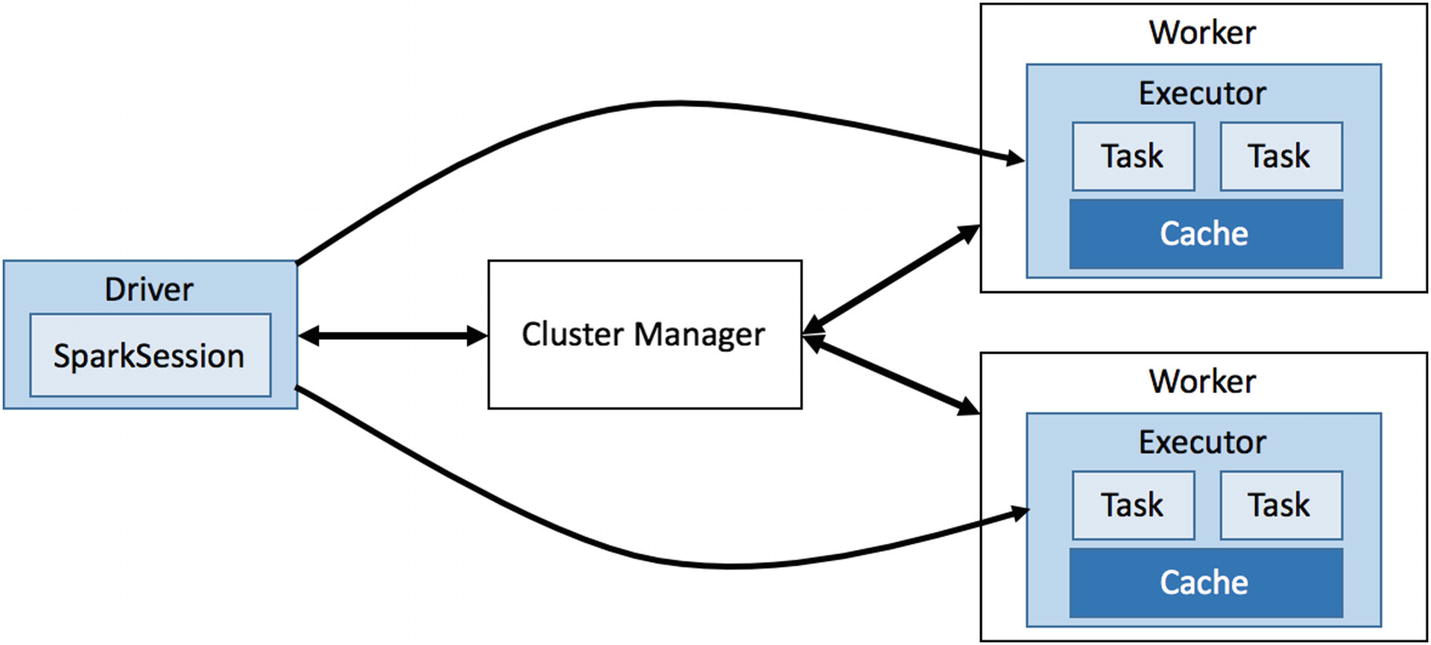
\includegraphics[width=0.7\linewidth]{illustrations/cluster-overview.jpg}
	\caption{ Interaction entre une application Spark et le cluster manager. Source : \cite{eginning-Apache-Spark-2-cluster-overwiew}}
	\label{fig:cluster-overview}
\end{figure}




\subparagraph{Application Spark} \label{sparkpresentationsection}
Une application Spark consiste en deux parties. La première partie concerne la logique décrivant les traitements à appliquer sur les données.  Cette logique est décrite en utilisant les APIs\footnote{API en Java, Scala, Python ou R.} disponibles. La deuxième partie est appelée le \textit{driver}, c'est le coordinateur principal d'une application Spark. Le driver interagit avec le cluster manager afin de trouver les machines sur lesquelles le traitement de données doit être réalisé. Ainsi, pour chacune de ces machines, le driver Spark lance le processus \textit{executor} en passant par le cluster manager. Un autre rôle du  driver Spark est de gérer et de distribuer les tâches Spark en provenance de l'application Spark sur chaque executor. Pour précision , dans la Figure \ref{fig:cluster-overview}, la classe \textit{SparkSession} est le point d'entrée vers une application Spark.

\subparagraph{Spark driver et executor}

Chaque Spark \textit{executor} est alloué exclusivement à une application Spark spécifique et la durée de vie d'un \textit{executor} est celle de l'application Spark. 

Spark utilise l'architecture master-slave. Spark \textit{driver} est le master et Spark \textit{executor} est le slave. De ce fait, une application Spark n'a qu'un seul Spark driver et plusieurs Spark \textit{executors}. Chaque Spark \textit{executor} s'occupe d'un traitement  sur une partie  des données à analyser. De cette manière,  Spark est capable de traiter  les données de façon parallèle. 
%La Figure \ref{fig:small-cluster-3} illustre un exemple d'un cluster. Ce dernier est composé de trois \textit{executors}.
%\begin{figure}[H]
%	\centering
%	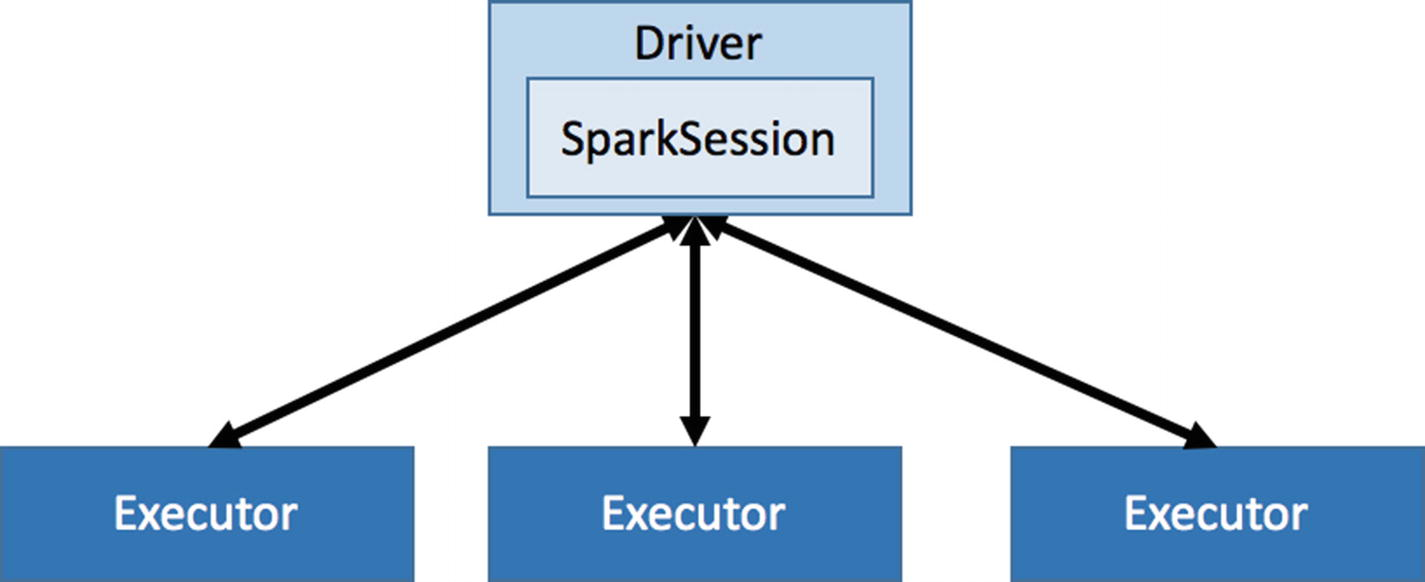
\includegraphics[width=0.7\linewidth]{illustrations/small-cluster-3}
%	\caption{Un exemple d'un cluster formé de trois executors. Source : \cite{eginning-Apache-Spark-2-cluster-example}}
%	\label{fig:small-cluster-3}
%\end{figure}


\subparagraph{Spark Unified Stack} \label{Spark Uniffied-Stack}Spark offre ce qu'on appelle Spark \textit{Stack}. C'est un ensemble de composantes construites au dessus de la composante Spark Core.  Ces composantes sont conçues pour répondre à des besoins spécifiques :
\begin{itemize}
	\item Spark SQL  est conçu effectuer des traitements sur des données structurées. Les traitements s'effectuent en se basant sur des requêtes SQL;
	\item Spark Streaming est utilisé pour les traitements    en temps réel des données en flux;
	\item  GraphX est destiné au traitement de graphes. Des fonctionnalités sont offertes afin d'analyser les graphes;
	\item MLib est conçu pour le machine learning. Ceci inclut la disponibilité des différents algorithmes et utilitaire du machine learning. Par exemple, les algorithmes de clustering, la classification, etc;
	\item SparkR est consacré aux traitements liés au machine learning en utilisant  R.
\end{itemize}
\subparagraph{Spark Core} est la base du moteur Spark pour le traitement distribué de données.  On distingue deux parties formant Spark Core. Premièrement, la partie concernant l'infrastructure distribuée du calcul. Cette dernière est responsable de la distribution, de la coordination et de la planification des tâches  sur les différentes machines formant le cluster. De plus, cette partie gère l'échec d'un traitement donné et le transfert de données entre les machines. Le deuxième élément formant Spark Core est appelé RDD (Resilient Distributed Dataset). Un RDD est une collection partitionnée d'objets, tolérante aux pannes et en lecture seule. 
%La Figure \ref{fig:unified-stack}  présente les différentes entités du Spark Unified Stack avec Spark Core.
%\begin{figure}[H]
%	\centering
%	\captionsetup{justification=centering}
%	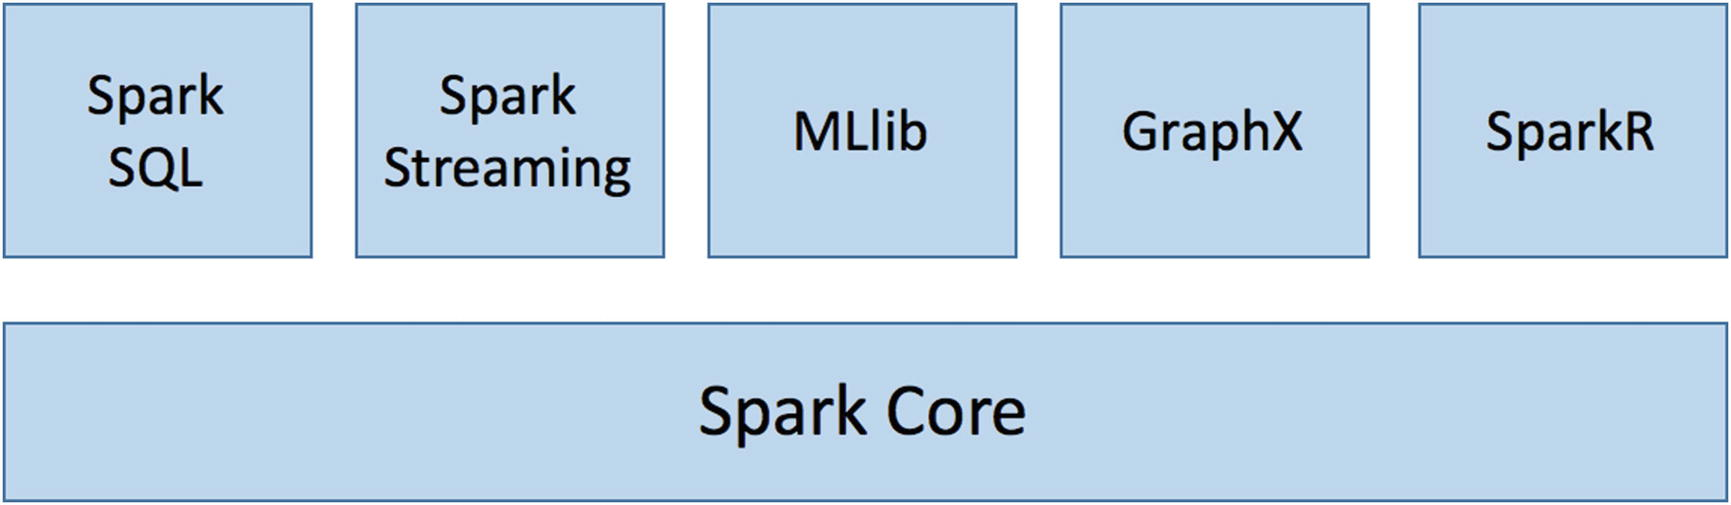
\includegraphics[width=0.7\linewidth]{illustrations/unified-stack}
%	\caption{ Spark Unified Stack. Source : \cite{eginning-Apache-Spark-2-unified-stack}}
%	\label{fig:unified-stack}
%\end{figure}

\paragraph{Resilient Distributed Datasets}\label{rdd-presentation} ~


Spark dispose d'une abstraction notée Resilient Distributed Datasets (ou RDDs). Un RDD est une collection d'objets immuable. Ces objets sont répartis sur les n\oe{}uds du cluster afin d'être traités en parallèle. Un RDD peut être conservé  pour une éventuelle réutilisation. On distingue deux manières de persistance. La conservation du RDD dans la mémoire (in-memory) ce que garantit l'amélioration des performances. En outre, un RDD peut être aussi conservé dans un disque. 

Les RDDs supportent deux types d'opérations sur les objets stockés : les transformations et les actions. Une  transformation appliquée sur un RDD crée un nouveau RDD, par exemple la transformation \textit{filter} retourne un RDD ayant vérifié la condition donnée en entrée.  Pour les actions, une action appliquée sur un RDD retourne une seule valeur, par exemple l'action \textit{count} compte le nombre d'objets d'un RDD.



%Dans la Figure 	\ref{fig:globalviewrdd}, Input data représente  les données à analyser en utilisant Spark. Ces données sont récupérées depuis des sources extérieures vers Spark. Ce dernier crée un RDD basé sur ces données. Un RDD est représenté par le rectangle en orange, les morceaux en orange dans le rectangle représentent les partitions d'un RDD. 
%On peut enchaîner plusieurs transformations sur un RDD. Comme une transformation est à la base  \textit{lazy}, les partitions ne sont partagées sur les n\oe{}uds du cluster qu'à la suite de l'appel d'une action. Une fois qu'une partition est localisée sur un n\oe{}ud donné, les transformations ainsi que les actions peuvent s'enchaîner.


 La Figure 	\ref{fig:globalviewrdd} illustre un flux de données avec l'utilisation de Spark. Dans cette figure, \textit{input data} représente les données qu'on souhaite analyser. Ces dernières sont en provenance de sources de stockage externes. Le framework Spark crée le RDD représenté par le premier rectangle orange à gauche. Ce dernier  comprend  des petits rectangles chacun représente une partition du RDD.  Les transformations  peuvent être enchaînées sur le RDD créé sans être exécutées. Les partitions seront envoyées à travers les n\oe{}ds dés que le \textit{driver} appelle une action sur ce RDD. Un n\oe{}ud est une machine avec des ressources de stockage (\textit{disk}), de calcul (\textit{CPU}), etc. Enfin, le reste des opérations peuvent s'enchaîner  sur chaque n\oe{}ud où se trouvent les données.

En cas de perte de partition pour une raison ou une autre, Spark est capable de reproduire automatiquement la partition en question. Cette fonctionnalité est assurée via le DAG (Direct Acyclic Graph). Dans ce graphe, Spark enregistre toutes les opérations appliquées sur un RDD.

\begin{figure}[h]
	\centering
	\captionsetup{justification= centering}
	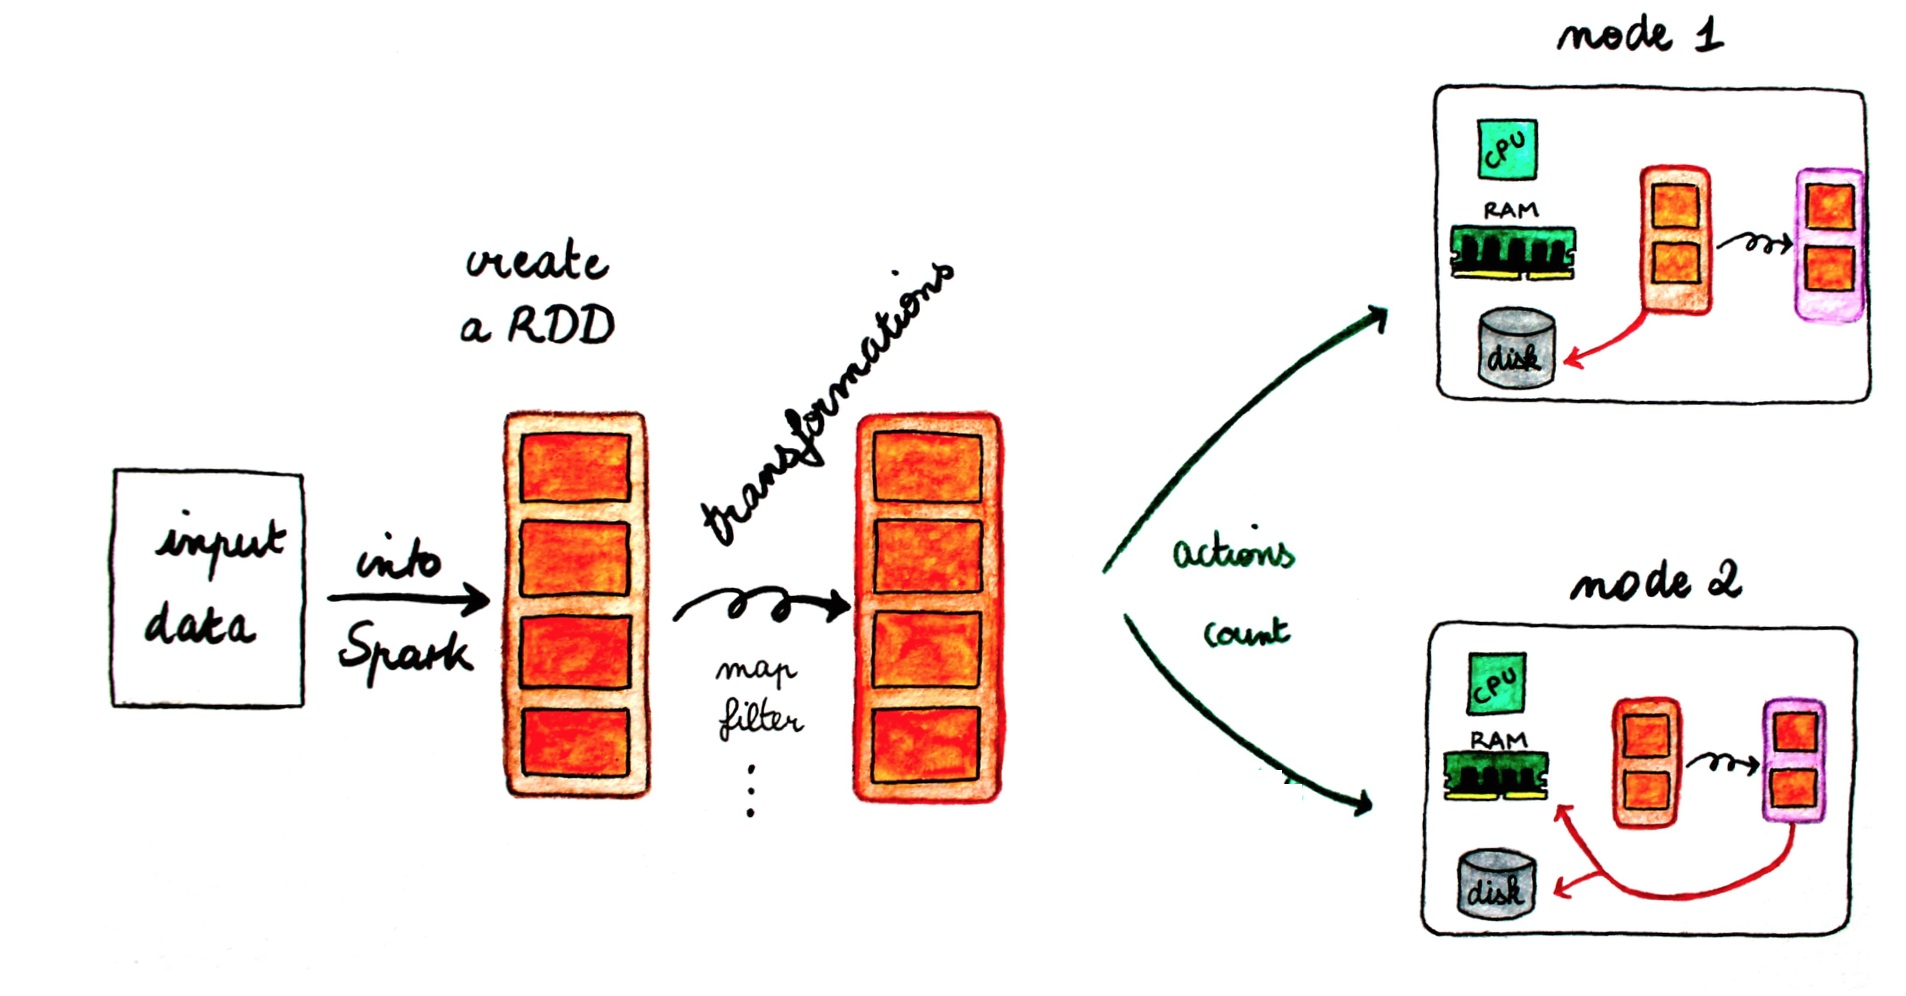
\includegraphics[width=0.7\linewidth]{illustrations/global_view_rdd}
	\caption{Exemple d'un flux de données avec Spark}
	\label{fig:globalviewrdd}
	\source{ \url{https://www.duchess-france.org/starting-with-spark-in-practice/}, consultée le $15/12/2018$.}
\end{figure}

%Resilient Distributed Dataset (RDD) allows Spark to transparently store data on the memory, and send to disk only what’s important or needed. As a result, a lot of time that is spent on the disc read and write is saved.

%Le RDD (Resilient Distributed Dataset) permet à Spark de stocker des données de manière transparente dans la mémoire et d’envoyer sur disque uniquement ce qui est important ou nécessaire. En conséquence, une grande partie du temps consacré à la lecture et à l'écriture du disque est enregistrée.[!]

\paragraph{Lazy evaluation} \label{lazy-evaluation}
Une transformation en Spark est considérée comme \textit{lazy}. Ceci implique que lorsqu'on exécute des fonctions de transformation en Spark, celles-ci ne sont pas exécutées de suite. Par contre, elles sont enregistrées dans le graphe (DAG).  Les transformations sont exécutées une fois le \textit{driver} invoque un appel à une fonction de type action. \textit{Lazy} ou l'évaluation paresseuse est un mécanisme permettant d'éviter le chargement de données depuis la source tant que ceci n'est pas nécessaire. Par conséquent, cela peut améliorer considérablement les performances.


 




%\paragraph{Les APIs de Spark}

%Le framework Spark a été écrit en Scala.  Il existe plusieurs APIs pour utiliser les fonctionnalités fournies par ce framework : Scala, Python, Java et R. 
%Il n'est pas évident de choisir entre ces quatre langages, car ce choix dépend du contexte de l'analyse. 


%Nous allons comparer ces langages dans le contexte du Big Data.



\paragraph{Les APIs du Spark}~

Spark dispose des APIs standards permettant aux développeurs  de créer une application Spark. Il existe une API en Scala, Python, Java et R. 

\paragraph{Lancement d'une application avec de Spark} \label{spark-master-modes}~

%Afin de pouvoir exécuter une application Spark, il faut l'installer. 
On distingue deux modes d'exécution d'une application  Spark : cluster et local. En  mode local, l'application  peut être exécuté au sein d'une machine locale. Par exemple,  avec un seul \textit{worker} thread (aucun parallélisme),  en précisant $K$ \textit{worker} sur $K$ threads, idéalement $K$ est le nombre des  c\oe{}urs de la machine sur laquelle Spark est installé, etc. 
 Pour le mode cluster, on distingue plusieurs types de clusters. Ces derniers  varient suivant le gestionnaire de ressources qui assure la communication entre les différentes entités du cluster selon le principe master-slave. Par exemple Hadoop YARN\footnote{URL : \url{https://hadoop.apache.org/docs/current/hadoop-yarn/hadoop-yarn-site/YARN.html}, consulté  le $14/05/2019$ } et Apache Mesos\footnote{URL : \url{https://mesos.apache.org/}, consulté le $14/05/2019$.}. La liste détaillée des alternatives pour chaque mode est donnée dans le site Web de Spark\footnote{URL : \url{https://spark.apache.org/docs/latest/submitting-applications.html\#master-urls}, consulté le $14/05/2019$.}. 
 
Il est possible d'installer Spark dans un cluster Amazon EMR (Elastic MapReduce)\footnote{URL  : \url{https://aws.amazon.com/fr/emr/}, consulté le $08/05/2019$.}. Par défaut, ce cluster utilise YARN comme gestionnaire de ressources.

\paragraph{Apache Spark VS Apache Hadoop}

Hadoop MapReduce est considéré dans \cite{Global-Journals} comme étant moins rapide en le comparant au framework Apache Spark.  Une étude \cite{article-comparaison-spark-hadoop} comparative entre Hadoop MapReduce et Spark a montré que Spark est $ 3 $ à $ 4 $ fois rapide que Hadoop MapReduce.
 Ceci est dû au fait que Spark traite les données suivant l'approche in-memory. Tandis que  les traitements basés sur le framework Hadoop sont basés sur des lectures/écritures sur le disque.  
%http://csjournals.com/IJCSC/PDF7-2/13.%20JP.pdf
\subsection{Amazon Elastic MapReduce} \label{emr-aws-presentation}

Amazon Elastic MapReduce\footnote{URL : \url{https://docs.aws.amazon.com/fr_fr/emr/}, onsulté le $10/05/2019$.} (EMR) est  un service Web proposé par Amazon  destiné aux traitements des données massives en utilisant Apache Hadoop, Apache Spark et autres.
Amazon EMR distribue le traitement de données à travers un cluster  de machines virtuelles redimensionnable. Ces machines sont des instances de type Amazon EC2\footnote{URL : \url{https://aws.amazon.com/ec2/}, consulté le $14/05/2019$.}.
Il existe plusieurs variantes d'instances EC2. Les instances sont conçues pour répondre 
aux besoins classés par AWS dans les catégories suivantes : usage général, calcul optimisé, calcul accéléré et stockage optimisé.
Elles se varient suivant leurs caractéristiques techniques comme la  RAM disponible, le nombre de CPUs, le nombre de c\oe{}urs physiques, etc. Les coûts d'utilisation des instances EC2 dépendent de ces caractéristiques,  de la région où se trouvent ces instances et du temps d'utilisation. Le coût d'utilisation des instances EC2 indépendamment d'EMR est différent du cas où une instance est utilisée pour former un cluster EMR.

Par défaut, Amazon EMR utilise YARN pour gérer les ressources. On distingue trois types de n\oe{}uds dans Amazon EMR. 
\begin{itemize}
	\item N\oe{}ud principal (\textit{Master node}) : il gère le cluster.
	\item N\oe{}ud de noyau (\textit{Core node}): exécute les tâches et stocke les données dans le système de fichier distribué Hadoop HDFS sur le cluster.
	\item N\oe{}ud de  tâche (\textit{Task node}) : il exécute les tâches et ne stocke pas les données dans HDFS. Les n\oe{}uds de tâches sont facultatifs.
\end{itemize}

Les coûts appliqués  à l'utilisation du service Amazon EMR dépendent des caractéristiques techniques des entités du cluster, la région d'Amazon choisie du cluster et enfin le temps d'utilisation du cluster. Il est possible d'estimer les frais d'utilisation d'Amazon EMR via le calculateur disponible sur le site Web d'Amazon\footnote{URL : \url{https://calculator.s3.amazonaws.com/index.html\#s=EMR}, consultée le $14/05/2019$.}.


\section{Conclusion}

Dans ce chapitre,  nous avons décrit brièvement  quelques technologies du Big Data, car la liste de toutes les technologies est très longue. Afin de découvrir ces technologies en pratique, nous allons aborder dans le chapitre \ref{chap:application-on-traceroutes} l'utilisation de ces technologies dans le cas de l'analyse des délais d'un lien décrite dans la chapitre \ref{chap:algorith-detection}.    










\chapter{Implémentations  } \label{chapter-implementations}


\section{Implémentation avec MongoDB}

MongoDB est la technologie Big Data utilisée par  Fontugne et al.  dans l'implémentation de l'outil de détection \cite{InternetHealthReport}. 
%MongoDB est une technologie conçue pour assurer  le stockage de données dans un processus d'analyse de données.
Dans MongoDB, les traceroutes sont organisés  dans des collections.  Par convention,  $V$  vaut $6$ s'il s'agit de l'adressage IPv6 et est vide dans le cas de l'adressage IPv4.  Le nom d'une collection est structuré comme suit: 	$tracerouteV\_YYYY\_MM\_DD$. La nomenclature  des collections permet de ne récupérer que les traceroutes concernés par l'analyse lancée.
L'implémentation détaillée de l'outil de détection est disponible sur GitHub \cite{InternetHealthReport}.  

En faisant appel à d'autres fonctions, les deux fonctions 
On note les deux fonctions \footnote{Voir l'implémentation des deux fonctions sur : \url{https://github.com/InternetHealthReport/tartiflette/blob/master/analysis/plot.py}, consulté le consulté le $ 02/02/2018$.} principales qui permettent de tracer l'évolution du délais des liens sont  :  

\textit{\textbf{getRttData(configFile=None)}} : en se basant sur les paramètres indiqués à travers le fichier de configuration \textit{configFile}, les traceroutes sont analysés. Cette fonction renvoie les liens identifiés avec leurs RTTs différentiels.

\textit{\textbf{rttEvolution(res, ips, suffix)}} : cette fonction prend en paramètre \textit{res} qui représente les détails du lien : les périodes de l'analyse, les RTTs différentiels qui correspondent à chaque période et les sondes ayant identifié ce RTT différentiel. Le paramètre \textit{ips} représente un lien; les deux adresses IPs.  \textit{suffix} n'a pas été utilisé dans la fonction.



Avec MongoDB,  la manière d'organiser les données dans des collections est importante pour assurer l'optimalité de la récupération des données. Dans l'implémentation de référence, chaque collection reprend les traceroutes d'une journée peu importe leur destination. Avec une fenêtre d'une heure et d'une journée d'analyse,  une même collection est consultée $24$ fois.   Or, si les collections ont été créées de sorte à contenir une heure de traceroutes, ceci aurait réduit la consultation des données inutilement dans le cas où la fenêtre est d'une heure, mais aussi pour les fenêtres de plus d'une heure. 

De plus, en partant du fait qu'une collection reprend une journée de traceroute, le choix de la taille de la fenêtre peut amener à négliger des traceroutes. Par exemple, si \textit{timeWindow} vaut   $ 4600 $ secondes et l'analyse s'étale sur $2$ journée, selon l'implémentation de référence, les traceroutes relatifs à la période entre  \textit{07/02/2018 23:00} et \textit{07/02/2018 00:15}   sont recherchés dans la collection  \textit{traceroute\_2018\_02\_07} et les traceroutes 
relatifs à la période entre \textit{08/02/2018 00:16} et \textit{08/02/2018 01:32}  sont recherchés dans la collection \textit{traceroute\_2018\_02\_08}. Dans ce cas, les traceroutes entre \textit{08/02/2018 00:00} et \textit{08/02/2018 00:15} sont négligés.

En ce qui concerne la capacité de  stockage d'une base de données MongoDB,  si les ressources de la machine locale où MongoDB est installé sont insuffisantes, il existe la version cloud de MongoDB (MongoDB Atlas). 



\section{Implémentation avec Amazon S3 et Amazon Athena} \label{implementation-athena}

%\paragraph{Application sur les traceroutes}~

\paragraph{Vue générale}~

Les trois services d'Amazon (Amazon S3, Amazon Glue  et Amazon Athena) ont été combinés  afin de créer un environnement d'analyse de données massives. 
Un des scénarios possibles mettant en pratique ensemble ces trois services est illustré dans la Figure
\ref{fig:gluecrawler}\footnote{Amazon Redshift  est un entrepôt de données et  Amazon Quicksight  est un service cloud d'informatique décisionnelle.}. Les  détails concernant chaque services sont donnés dans les sections suivantes.

Afin d'utiliser Amazon Athena pour l'interrogation des traceroutes stockés dans des fichiers, il faut d'abord  stocker ces fichiers dans Amazon S3. De plus, il faut créer un  schéma de données. Il s'agit de créer une table comme les tables dans un SGBDR. Chaque enregistrement dans cette table correspond à une ligne dans les fichiers de données censés être lus par cette table. Il existe deux manières pour créer une table dans Athena : en utilisant Amazon Glue ou création manuelle. \textit{traceroutes\_api} désigne le nom de la table reprenant tous les traceroutes.
%Une vue globale du  processus de l'analyse  est illustré dans la Figure  

\begin{figure}[h]
	\centering
	\captionsetup{justification=centering}
	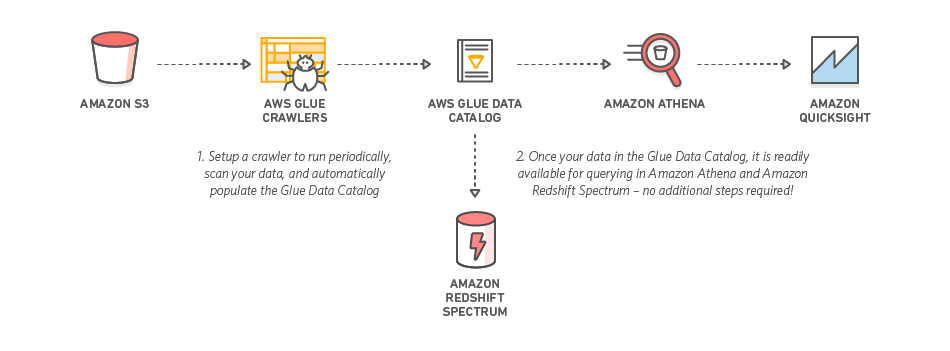
\includegraphics[width=1\linewidth]{illustrations/glue_crawler}
	\caption{Une combinaison des services web d'Amazon : Amazon S3, Amazon Glue, Amazon Athena, Amazon Quicksight  et Amazon Redshift}
	\label{fig:gluecrawler}
	\source{\url{https://docs.aws.amazon.com/fr_fr/athena/latest/ug/glue-best-practices.html}, consultée le $16/05/2018$.}
\end{figure}


\paragraph{Création de la table traceroutes avec Amazon Glue}~

Afin de découvrir rapidement le schéma des traceroutes,     la détection automatique du schéma a été lancées, avec Amazon Glue, sur un ensemble de  traceroutes enregistrés dans un fichier faisant une taille de $500$ MB. Toutefois, la détection a échoué. Autrement dit, Amazon Glue n'a pas pu inférer le schéma d'une seule table capable de lire tout traceroute dans ce fichier.  L'échec de l'inférence est dû au fait que le fichier contient des traceroutes différents en terme de structure, car la structure dépend de la version du firmware de la sonde ayant effectué le traceroute. Les différentes versions du firmware  pour chaque type de mesure sont détaillées dans le site Web d'Atlas\footnote{\url{https://atlas.ripe.net/docs/data_struct/}, consultée le $16/01/2018$.}.
%L'origine de cette différence  est le fait que ces traceroutes ont été effectués par des sondes ayant un firmware différent. Car le contenu des résultats d'une requête traceroute  et son organisation dans un objet JSON dépend partiellement du firmware de la sonde. 

\paragraph{Création manuelle de la table \textit{traceroutes\_api}}~ \label{creer-table-traceroute}

Suite à l'échec d'Amazon Glue  et comme la structure des réponses traceroutes est disponible,  la structure de la table a été créée   manuellement en se basant sur la structure détaillée d'une réponse traceroute pour chaque version du firmware. \textit{traceroutes\_api} dénote le nom de la table créée. Les différentes structures de réponses d'une requête traceroute n'ont posé aucun problème dans la création manuelle de la table. Dans notre cas, la réussite de la création manuelle est due au fait que les attributs dont l'outil de détection a besoin sont présents dans toutes les versions du firmware d'une part. D'autre part, Amazon Athena est flexible en ce qui concerne l'association entre un objet JSON et un enregistrement dans une table. Autrement dit, si un attribut existe dans l'objet JSON, la colonne correspondante prend sa valeur et vide dans le cas échéant.  

\subparagraph{Création de la table traceroutes } 
La création d'une table reprend plusieurs parties :
\begin{itemize}
	\item les colonnes de la table avec le type correspondant (int, string, array pour définir une liste, struct pour définir un objet );
	\item LOCATION : c'est l'endroit où les données sont stockées dans Amazon S3, il faut préciser le chemin vers le compartiment de données;
	\item ROW FORMAT SERDE : elle définit la manière dont chaque ligne d'un fichier de données est sérialisée/désérialisée par Amazon Athena;
	\item PARTITIONED BY : elle définit la manière dont les données sont organisées dans le compartiment de données; 
	\item WITH serdeproperties : elle définit les options de la sérialisation/désérialisation.
\end{itemize}
\begin{lstlisting}[language=SQL, basicstyle=\footnotesize, label=createAthenaTable, caption={Création de la table des traceroutes dans Amazon Athena }]
CREATE EXTERNAL TABLE traceroutes_api(
af int,
bundle int,
dst_addr string,
dst_name string,
fw int,
endtime int,
`from` string,
group_id int,
lts int,
msm_id int,
msm_name string,
paris_id int,
prb_id int,
proto string,
size int,
src_addr string,
`timestamp` int,
ttr float,
type string,
result array< struct< hop:int,error:string, result:array<
struct<x:string, err:string, `from`:string, ittl:int, edst:string, late:int, mtu:int, rtt:float, size:int, ttl:int , flags:string, dstoptsize:int, hbhoptsize:int, icmpext:
struct<version:int, rfc4884:int, obj:array< 
struct<class:int, type:int, mpls:array<struct< exp:int, label:int, s:int, ttl:int>>>>>>>>> 
)
PARTITIONED BY (
af_ string,
type_ string,
msm string ,
year string,
month string,
day string,
hour string
) 
ROW FORMAT SERDE 'org.openx.data.jsonserde.JsonSerDe'
WITH serdeproperties ('paths'='af,bundle,dst_addr, dst_name,fw, endtime, from, lts, msm_id, paris_id, prb_id, proto, size, src_addr, timestamp, type,fw, msm_name' ) 
LOCATION 's3://ripeatlasdata/traceroute/source=api/'
\end{lstlisting}





\paragraph{Partitionnement des données stockées dans Amazon S3}~

La table \textit{traceroutes\_api} créée a été conçue de sorte qu'elle prenne en compte  le partitionnement de données dans un compartiment S3 dans la création de la table \textit{traceroutes\_api}.  L'utilisation du partitionnement est optionnel. 
Il permet de limiter la quantité de données à analyser par une requête Amazon Athena. Le partitionnement améliore donc les performances d'Amazon Athena. D'une part, la requête s'exécute plus rapidement. D'autre part, il réduit les coûts engendrés  suite à l'utilisation d'Amazon Athena, car ce dernier est facturé selon la quantité de données analysées. En pratique,  une partition créée joue un rôle similaire à celui d'une colonne durant l'interrogation d'une table dans Athena. 

Prenons un exemple illustrant l'apport du partitionnement. Nous avons des traceroutes effectué en adressage IP  version  $ 4 $ et $ 6 $.


\textit{af\_} désigne le type d'adressage : \textit{af\_} vaut $4$ en cas d'adressage IPv4 et $6$ en cas d'adressage IPv6. Sans l'utilisation du partitionnement et si on ne souhaite récupérer que  les traceroutes ayant comme adressage IPv4, tous les traceroutes présents dans le compartiment S3 (appelé \textit{s3://ripeatlasdata}) sont évalués.
%\footnote{L'évaluation du type  d'adressage est effectué selon la valeur de l'attribut \textit{af} d'un traceroute, il vaut \textit{4} ou \textit{6}.}.

Toutefois, en partitionnant les données suivant par exemple le type d'adressage, seuls les fichiers dans la partition
%\footnote{Partition dans le sens d'Amazon Athena.} 
af\_ = $4$  sont analysés. Par conséquent, le partitionnement permet de réduire les coûts d'utilisation du service Amazon Athena, surtout si la quantité de données est très importante. 


Les partitions   créées sont illustrées  dans la Figure 	\ref{fig:partitionnement-athenaa}. Ces partitions ont été créées manuellement. Le choix des partitions à créer  dépend de l'interrogation des données; des paramètres de la requête SQL conçue pour récupérer  les données. Par exemple, si toutes les requêtes SQL  sont indifférentes concernant la version IP, il n'est pas nécessaire de créer la partition af\_. Pour précision, le partitionnement permet  d'organiser les données en une structure de répertoires hiérarchique. Les valeurs de chaque partition sont distinctes.
Le  Tableau \ref{tab:partition-description} 
reprend les  partitions créés.  La première colonne représente le nom de la partition, dans 
la deuxième colonne on donne quelques valeurs de chaque partition et la troisième colonne de ce tableau reprend la description de la partition.

\begin{figure}[h]
	\centering
	\captionsetup{justification=centering}
	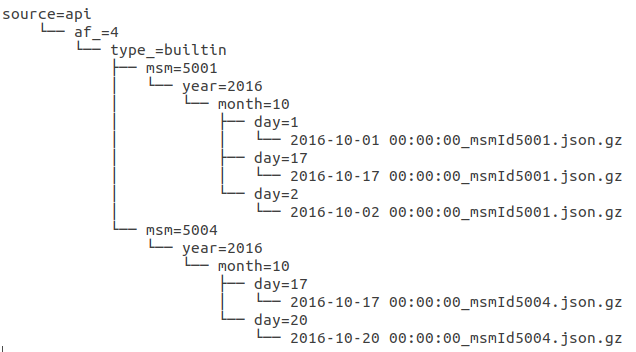
\includegraphics[width=1\linewidth]{illustrations/partitionnement-athena}
	\caption{L'organisation des traceroutes dans le compartiment Amazon S3 \textit{s3://ripeatlasdata}}
	\label{fig:partitionnement-athenaa}
\end{figure}

\begin{table}[h]
	\centering
	\captionsetup{justification=centering}
	\begin{tabular}{|c|c|l|}
		\hline 
		\textbf{partition}	& \textbf{Valeurs} & \multicolumn{1}{c|}{\textbf{Commentaires} }\\ 
		\hline 
		source& api & Les  traceroutes récupérés depuis le dépôt  d'Atlas via l'API \\ 
		\cline{2-3}
		&typeanddate& Les  traceroutes récupérés depuis la page Web\\
		\hline 
		af\_& 4  & Les traceroutes en adressage IPv4 \\ 
		\cline{2-3} &6& Les traceroutes en adressage IPv6\\	\hline 
		type& builtin  & Les traceroutes en provenances des mesures intégrées \\ 
		\cline{2-3} 
		&anchor& Les traceroutes à destinations des ancres\\ \hline
		msm& 5001 & Les traceroutes ayant msm\_id = 5001 \\ 
		\cline{2-3}  &5004& Les traceroutes ayant msm\_id = 5001 \\
		\hline 
		year& 2016 & Les traceroutes effectués en $2016$ \\ 
		\hline 
		month& 10 & Les traceroutes effectués en octobre \\ 
		\hline 
		day& 1 & Les traceroutes effectué le premier du mois \\ 
		\hline 
	\end{tabular}
	\caption{Exemple des partitions créées dans un compartiment Amazon S3} 
	\label{tab:partition-description}
\end{table}

Les   partitions \textit{af\_} et \textit{type\_} sont nommées de cette manière, au lieu de \textit{af} et \textit{type} car  la table \textit{traceroutes\_api} contient des colonnes avec ces noms et comme les partitions agissent comme des colonnes  lors de l'évaluation d'une requêtes avec Amazon Athena, les noms de ces partitions ont été adaptés.

Par exemple, les traceroutes qui se trouvent dans  le fichier\\
\textit{2016-10-01 00:00:00\_msmId5001.json.gz} sont analysés par toute requête SQL Athena  
impliquant les partitions d'une des manières énumérées dans le Tableau \ref{partitions-sql}.

\begin{table}[H]
	\resizebox{\textwidth}{!}{
		\begin{tabular}{l}
			\textbf{Prédicat} \\ \hline
			(source = api) \\ \hline
			(source = api et af\_ = 4)\\ \hline
			(source = api et af\_ = 4 et type = builtin) \\ \hline
			(source = api et af\_ = 4 et type = builtin et msm = 5001) \\ \hline
			(source = api et af\_ = 4 et type = builtin et msm = 5001 et year = 2016) \\ \hline
			(source = api et af\_ = 4 et type = builtin et msm = 5001 et year = 2016 et month = 10) \\\hline
			(source = api et af\_ = 4 et type = builtin et msm = 5001 et year = 2016 et month = 10 et day = 1)\\ \hline
		\end{tabular}
	}
	\caption{Exemple d'utilisation des partitions dans une requête SQL dans Amazon Athena}
	\label{partitions-sql}
\end{table}
\paragraph{Interrogation des données Avec Amazon Athena}~  \label{sql-athena-request}

Une fois les fichiers de données  synchronisés vers le compartiment AWS S3 et le schéma  de données  créé, on passe à l'interrogation de données en utilisant les requêtes SQL basées sur Presto.  On peut décomposer une requête SQL en trois parties principales:

\begin{description}
	\item[Les données sollicitées] Ça peut être une colonne ou bien bien une colonne transformée suite à l'application d'une ou de plusieurs fonctions de Presto.
	\item[Les partitions de données concernées] La requête SQL est paramétrée de sorte à limiter les données à analyser sur Amazon S3. 
	\item[Les paramètres appliqués sur les colonnes] La requête SQL doit filtrer les données suivant les conditions sur les colonnes de la table.
\end{description}

La Figure \ref{fig:sqlrequestathena} montre  un exemple d'une  requête SQL dans Athena.  Cette requête fait appel aux fonctionnalités  de Presto\footnote{URL : \url{https://prestodb.github.io/docs/current/}, consulté le $10/06/2018$.} comme  \textit{transform}, \textit{concat}, etc. 
Pour les données sollicitées, ce sont les trois colonnes \textit{prb\_id}, \textit{from}, \textit{msm\_id} (ligne $2$)et la liste de saut (\textit{hops})obtenue après quelques vérifications (lignes $3$ à $9$). A la ligne $10$, c'est la table créée pour les traceroutes (voir les détails de la table dans \ref{createAthenaTable}). Les traceroutes à analyser sont ceux obtenus en vérifiant les conditions dans la ligne  $12$ et $13$. C'est à dire, Athena va regarder les traceroutes qui se trouvent dans les sous dossiers year=2016/month=10/day=21 qui se trouvent aussi dans les deux dossiers msm=5001 et msm=5004. Ce que revient à chercher les traceroutes dans les deux endroits suivants:

\begin{lstlisting}[basicstyle= \footnotesize]
s3://ripeatlasdata/traceroute/source=api/af_=4/type_=builtin/msm=5001/year=2016/month=10/day=21
s3://ripeatlasdata/traceroute/source=api/af_=4/type_=builtin/msm=5004/year=2016/month=10/day=21
\end{lstlisting}

Le choix des partitions est basé sur les identifiants des mesures indiquées dans les paramètres. Si aucun des identifiant n'est précisé, toutes les identifiants des mesures sont considérées. En ce qui concerne les partitions \textit{year}, \textit{month} et \textit{day}, leur valeur est inférée de la période en cours.

\begin{figure}[h]
	%	\resizebox{}{!}{
	\centering
	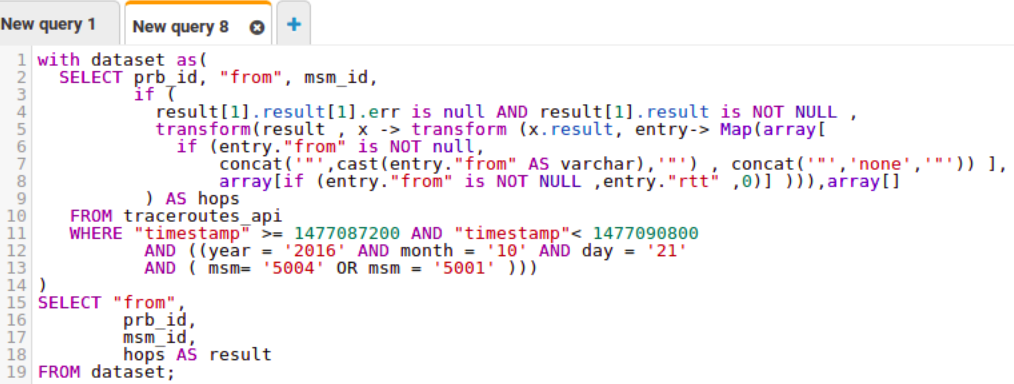
\includegraphics[width=1\linewidth]{illustrations/sqlRequestAthena2.png}
	\caption{Une exemple d'une requête SQL sur Amazon Athena}
	\label{fig:sqlrequestathena}
\end{figure}




\begin{comment}

\begin{table}[h]
	\begin{tabularx}{\linewidth}{lX}
     \textbf{Lignes}& \textbf{Commentaires}\\ \hline
     1 à 2 & : la clause  \textit{with} définit les relations nommées à utiliser dans une requête. \\  \hline
     3 à 8 & : vérifier la validité du traceroute.  Le premier \textit{result} contient la liste sauts, pour chaque saut, \textit{result} représente la liste des signaux. D'abord on vérifie la validité d'un traceroute, ensuite on transforme chaque signal (\textit{entry}) de la liste des signaux de chaque saut (\textit{x}) afin de ne récupérer que \textit{from} et \textit{rtt}. Les derniers sont entourés par "" pour faciliter le passage d'une réponse fournie par Amazon Athena à une structure de données manipulée en Python.   \\  \hline
     9 & : la colonne qui représente les sauts obtenus prennent le nom \textit{hops}.\\  \hline
     10 & indiquer la table Athena  contenant les traceroutes.\\  \hline
     11& : préciser la période concernée  \\  \hline
     12  à 13 & : préciser les partitions de données à consulter \\   \hline
     15 à 19 & : sélectionner les colonnes utiles. \\  \hline
	\end{tabularx}
\end{table}

\end{comment}
\paragraph{Intégration d'Amazon Athena dans l'outil de détection}~ \label{integration-aws-possibilite-une}


Pour intégrer Amazon Athena dans l'outil de détection \cite{InternetHealthReport}, on distingue deux possibilités. La première possibilité n'utilise Athena que pour récupérer  les traceroutes stockés dans Amazon S3 vers  la machine locale. Ensuite, cette dernière poursuit les traitements  décrits dans la phase I et II. Dans ce cas, nous ne profitons pas  des performances d'Amazon Athena vu que les traitements complexes sont effectués dans la machine locale.
%vérifiés en terme de validité; c'est l'objectif des étapes $1$ et $2$ dans le processus de la création de l'évolution des RTTs différentiels des liens (voir la section \ref{steps-rtt-analysis}).  
%Les traitements qui suivent (étapes  à partir de $3$) sont effectués dans la machine locale. Dans ce cas, l'utilisation des technologies  Big Data est limité qu'au niveau stockage de données massives. 

La deuxième possibilité vise la maximisation des traitements des  phases I et II au sein de l'infrastructure  d'Athena. De ce fait, la machine locale n'a qu'à recevoir les derniers résultats de la détection, voire les résultats finaux. Pour cette deuxième possibilité, les données doivent être manipulées de sorte à maximiser,  	au niveau d'Amazon Athena,  les traitements relatifs à toutes les étapes des  phases I et II. 

Pour la deuxième possibilité, le défi est de trouver la requête ou bien l'ensemble de requêtes SQL à exécuter sur Athena en vue d'avoir l'évolution du RTT différentiel des liens. 
Vu la complexité des  étapes des phases I et II, on ne peut pas trouver une seule requête SQL assurant toutes ces étapes à la fois. Supposons qu'il existe une requête SQL capable de trouver les liens possibles avec leurs RTTs différentiels : à l'étape $ 4 $ dans \ref{steps-rtt-analysis}, on construit la distribution des RTTs différentiels pour tout lien $l$ identifié dans les traceroutes de la période $d_k$. Cette distribution est mise à jour à chaque fois $l$ est identifié dans un des traceroutes  de la période $d_k$. 

Soient  $T_k$ = \{$t_{k, j}$\}  l'ensemble de traceroutes effectués durant $d_k$, avec $j \in [1, R_k]$ et $R_k$ est le nombre de traceroutes effectués durant $d_k$. Nous décrivons le parcours des traceroutes d'une période $d_k$ brièvement dans le pseudo-code \ref{alo-inference-link}. Nous n'avons pas donné  tous les détails, car l'objectif est d'évaluer la pertinence d'Athena au traitement souhaité.
\begin{algorithm}[H]
	\begin{algorithmic}[1]
		\ForAll{ $t_{k, j}$ $\in$ $T_k$} \
		\State $links$ $\leftarrow$ getLinksFromTraceroute($t_{k, j}$)
		\ForAll{$l$ $\in$ $links$}
		\State updateLinkRttDistribution($l$) \label{update-link}
		\EndFor
		\EndFor
	\end{algorithmic}
	\caption{Une partie de l'étape $4$ du processus de la détection des anomalies des délais }
	\label{alo-inference-link}
\end{algorithm}

Avec : 
\begin{itemize}
	\item \textit{getLinksFromTraceroute($t_{k, j}$)} énumère tous les liens possibles dans le traceroute $t_{k, j}$.
	
	\item \textit{updateLinkRttDistribution($l$)} ajoute le RTT différentiel calculé du lien $l$ à la distribution des RTTs différentiels courante de ce lien pour la période $d_k$.
\end{itemize}


Le service Athena est conçu pour la lecture de données, toute mise à jour de données n'est pas possible avec ce service. C'est pourquoi la distribution des RTTs différentiels de chaque  lien identifié doit être sauvegardée dans un endroit accessible en lecture et en écriture, par exemple dans un compartiment AWS S3. Que ce soit un fichier reprenant la distribution des RTTs différentiels  par un seul lien ou bien un fichier pour tous les liens,   à la ligne  \ref{update-link} du pseudo-code \ref{alo-inference-link}, un fichier doit être lu et mise à jour avec de nouvelle valeur. Pour une période $d_k$ d'une heure, le nombre de traceroutes est de l'ordre de milliers. Chaque traceroute $t_{k,j}$ peut inclure $L_{k,j}$ liens. Dans ce cas, le nombre total, d'une période $d_k$, de mise à jour de la distribution des RTTs différentiels est    $ \sum_{m=1}^{R_k}  L_{k,m}$. $ L_{k,j} $ dépend du nombre de saut du  traceroute $t_{k,j}$.

%de l'ordre $R_k$\texttimes$L$ de fois.  Cette estimation est à titre indicatif, de plus elle ne concerne que l'étape $4$, le nombre de lectures et/ou d'écritures dépend des requêtes SQL créées pour les autres étapes. 

En plus du nombre de lectures et d'écritures, relatives à la phase I, que nous venons de décrire, à la phase II, la détection des anomalies s'effectue en  comparant les intervalles de confiance. Cette comparaison révèle deux contraintes. La première contrainte concerne  la fonction permettant de calculer les deux bornes de l'intervalle de confiance de Wilson ne fait pas partie des fonctions disponibles sur Amazon Athena. D'autre part, Amazon Athena ne permet pas la création des fonctions personnalisées pour répondre à des besoins non couverts par Amazon Athena. La deuxième contrainte concerne la mise à jour de l'intervalle de confiance de référence qui doit être faite à chaque nouvelle période.


\paragraph{Evaluation des critères pour Amazon S3 et Amazon Athena  }~

Afin d'utiliser le service Amazon Athena à moindre coût, il est conseillé d'utiliser le partitionnement, car moins de frais sont appliqués. Si un partitionnement particulier est adopté, la création du schéma de données est basé sur ce partitionnement ainsi que les requêtes SQL destinés à l'interrogation de la table de données.

En ce qui concerne l'évolutivité d'une application basée sur ces deux services d'Amazon, on note que toute mise à jour de la structure de données des objets traceroutes peut affecter l'entièreté de la configuration initiale. A savoir, l'organisation des fichiers de données via le partitionnement, le schéma de données et les requêtes SQL.

Quant à la flexibilité du schéma de données, le service  Amazon Athena est tolérant au données manquantes. Etant donné que la structure d'un objet traceroute dépend de la version du firmware de la sonde, nous avons créé trois schémas de tables. La première table  modélise tout objet traceroute de  version $5$, la deuxième modélise tout objet traceroute de version $6$ et enfin la troisième table modélise ceux ayant la version $7$. En expérimentant différentes requêtes, nous avons conclu  que Amazon Athena a pu récupérer les données de la version récente ($7$) via le schéma de la version $5$ malgré que la version $7$ a plus d'attributs par rapport à la version $5$.




\section{Implémentation  en Spark/Scala} \label{application:spark}
\subsection{Introduction}

Ce chapitre  décrit  l'implémentation de l'outil de détection en utilisant le framework Spark, avec Scala comme API.  Dans un premier temps, nous présentons brièvement le langage Scala qui fait partie des langages de programmation fonctionnelle. Ensuite, nous 
décrivons les notre implémentation en Spar/Scala.

\subsection{Présentation de Scala} \label{scala-presentation}

%Nous allons présenter le langage Scala\footnote{Présentation basée sur \url{http://igm.univ-mlv.fr/~dr/XPOSE2011/le_langage_scala/}, consultée le $09/04/2019$}. 

La première version du langage Scala date de l'année $2003$, le terme  Scala  est dérivé de \textit{Scalable language}. 
La particularité de ce langage est le fait de proposer à la fois plusieurs avantages. Scala appartient à la 
programmation multi-paradigme, c'est  un langage à la fois orienté objet, il supporte la programmation fonctionnelle et fait partie des langages impératifs. En terme de compatibilité, Scala est interopérable avec  Java, car ce dernier est compilé en bytecode Java. Ceci permet d'utiliser du code Java avec le code Scala, de garantir l'indépendance des systèmes d'exploitation et d'utiliser la richesse des bibliothèques en Java. De plus, le code écrit en Scala est facile à lire.
Nous comparons dans le Listing \ref{java-vs-scala} l'écriture d'un même traitement écrit en Java et en Scala.
\begin{center}
	\begin{minipage}[t]{.50\textwidth}
\begin{lstlisting}[language=java, basicstyle=\small]
//Java
Integer[] intArray = {1,2,3,4,5};
List <Integer> numsList = Arrays.asList(intArray);
List <Integer> positves = new LinkedList < Integer > ();
for (int i: numsList) {
  if (i > 0) positives.add(n);
}
\end{lstlisting}
	\end{minipage}\hfill
	\begin{minipage}[t]{.49\textwidth}
\begin{lstlisting}[language=scala, basicstyle=\small]
// Scala 
val positives = List(1,2,3,4,5).filter(_ > 0)
\end{lstlisting}
	\end{minipage}
	\captionof{lstlisting}{Comparaison entre un traitement écrit en Java et en Scala}
	\label{java-vs-scala}
\end{center}
%L'implémentation proposée implique plusieurs éléments relatifs au langage Scala comme les case class, les fonctions et le RDD relatif au Spark. 

\paragraph{Notation relatives au langage Scala}~
Il existe plusieurs manières pour définir une fonction en Scala. Nous présentons celle utilisée dans les Listings du présent chapitre. Dans le Listing \ref{lst:generalFunction}, on crée une fonction appelée  \textit{functionName}, ayant deux paramètres : \textit{x} de type \textit{Int} et \textit{y} de type \textit{Int}, elle renvoie \textit{result} de type \textit{String}, le mot-clé \textit{return} est optionnel.  
\begin{lstlisting}[language=scala,firstnumber=1, caption={Exemple d'une fonction en  Scala}, label={lst:generalFunction}, basicstyle = \footnotesize,escapechar=|,numbers=left,
stepnumber=1,numberstyle=\scriptsize]
def functionName(x: Type, y Int): String = {
	// some  code that uses x and y and return result
	return result 
}
\end{lstlisting} \par

Nous présentons  des notations   propres au langage Scala. Ce  sont les mots clés utilisés  dans les Listings du présent chapitre. \par
\textbf{\textit{case class}} (mot-clé): définir une  classe.\par
\textit{\textbf{Seq}} (type): créer une séquence, équivalent à créer une liste. Par exemple Seq[String] représente le type d'une liste dont ses éléments sont de type String. Lors du parcours d'une séquence  l'élément courant est accessible via " \_".  \par
\textbf{\textit{Dataset}} (type):  est une collection distribuée de données. Elle est similaire à un RDD (voir la section \ref{rdd-presentation}) et plus récente que les RDDs. \par
\textit{\textbf{map}} (fonction): permet de transformer le contenu d'une liste en appelant une fonction sur chaque élément de la liste, elle renvoi une liste transformée. \par
\textit{\textbf{Option}} (type) : représente une valeur optionnelle.  \par
\textit{\textbf{groupBy}} (fonction):  est une fonction utilisée pour regrouper les éléments d'une liste (\textit{l\_0}) ayant une clé en commun (\textit{key}). Cette fonction renvoie une liste de tuples. Chaque tuple (\textit{tup})  contient deux éléments. Le premier représente la clé (\textit{key})  du groupement, son contenu est accessible via \textit{tup.\_1}. Le deuxième élément est une liste d'éléments de \textit{l\_0} ayant la même clé, son contenu est accessible via \textit{tup.\_2}.\par
\textbf{\textit{List}} (type): créer une liste d'un type donné. La liste \textit{l\_1} de deux chaînes de caractères est créée comme suit:
\begin{lstlisting}[language=scala,firstnumber=1,label={lst:case-class-hop}, basicstyle = \footnotesize,escapechar=|,numbers=left,
stepnumber=1]
l_1: List[Int] = List("aa", "bb")
\end{lstlisting} \par
\noindent \textbf{\textit{filter}} (fonction): cette fonction permet de filtrer les éléments d'une collection pour créer une nouvelle collection contenant uniquement les éléments de la collection   vérifiant une condition. Prenons un  exemple : 
\begin{lstlisting}[language=scala,firstnumber=1, basicstyle = \footnotesize,escapechar=|,numbers=left,
stepnumber=1]
//créer une liste d'entiers entre 1 et 10, l_2 vaut List(1, 2, 3, 4, 5, 6, 7, 8, 9)
val l_2 = List.range(1, 10)   
// filter les éléments de l_2 afin de ne garder que ceux paires, evens vaut List(2, 4, 6, 8)
val evens = l_2.filter(_ % 2 == 0)  
\end{lstlisting} \par

\textit{\textbf{collect}} (fonction): c'est une fonction liée au fonctionnement de Spark plutôt qu'au Scala, précisément, elle est appelée à partir d'un RDD.    La fonction \textit{collect} ramène la totalité des données traitées par les \textit{workers} vers le driver.\par

\textit{\textbf{flatten}} (fonction): la méthode \textit{flatten}  prend une liste de listes et concatène toutes les listes d'éléments de la liste principale afin de retourner une seule liste reprenant tous les éléments. 
%Autrement dit, la fonction \textit{flatten} prend A[A[T]] et retourne A[T], T est type de données et A peut être List, Seq, etc.

\subsection{La programmation fonctionnelle et le Big Data}
%\subsection{Les apports de la programmation fonctionnelle}

La programmation fonctionnelle est un style de programmation où l'évaluation se base sur les fonctions.  La programmation fonctionnelle se caractérise par les éléments suivants \cite{bigdatafunctional} :

\textbf{Fonctions d'ordre supérieur} ou  \textit{higher-order} functions en anglais. Dans un langage, si une fonction est traitée comme first-class value, elle est considérée comme fonction d'ordre supérieur \cite{DBLP:journals/csur/Hudak89}.
\begin{tcolorbox}
	\textbf{First-class functions}: ou fonctions de première classe dans un langage de programmation sont des fonctions qui peuvent être stockées dans des structures de données, peuvent être passées comme arguments aux fonctions et être retournées comme résultats.
\end{tcolorbox}
\par
\textbf{Structures de données immuables.} Un objet est immuable est celui qu'on ne peut pas changer son état après sa création. \par
\textbf{Stateless} ou \textit{no side effect} en anglais.  Une fonction est dite n'ayant pas  l'effet de bord, quand cette fonction ne modifie pas une variable en dehors de son environnement local. Par exemple, les fonctions qui modifient l'état d'une variable passée à cette fonction par référence sont considérées comme ayant un effet de bord.\par
%\subsection{La programmation fonctionnelle au service du Big Data }

Quand il s'agit des traitements appliqués sur des données massives dépassant la capacité d'une seule machine, la distribution de ces traitements sur plus d'une machine  est nécessaire. La programmation fonctionnelle peut apporter des facilités aux projets Big Data. 
En particulier, l'absence d'effet de bord lors de la conception des fonction est un élément clé pour faciliter la parallélisation des traitements appliqués sur des volumes importants de données. Ceci permet aussi de mieux gérer les opérations concurrentielles. 
La manipulation des structures de données immuables permet d'écrire un code lisible grâce au nombre réduit de dépendances sur ces structures. De plus, les structures de données immuables facilitent la parallélisation, car elles supportent seulement le mode lecture-seule.

%On distingue deux sous-catégories de langages de programmation fonctionnelle. Des langages qui sont purement fonctionnels et les autres hybrides.
%La programmation fonctionnelle offre de nombreux avantages dans un contexte Big Data. 



\subsection{Implémentation détaillée }
\subsubsection{Description de l'environnement}
%Spark est destiné aux traitements distribués sur un cluster de machines, toutefois,n
La création d'une application Spark/Scala implique  les étapes suivantes:
\begin{itemize}
	\item gérer les dépendances nécessaires au fonctionnement de l'application avec le fichier de modèle objet du projet (POM);
	\item écrire l'application en Scala;
	\item créer le fichier JAR de l'application Spark;
	 \item Soumettre  l'application  au cluster de machines. 
\end{itemize}

L'implémentation proposée est adaptée au mode local de Spark  ainsi qu'au  mode cluster. 
Le code source, qui traduit l'ensemble des traitements, est organisé dans une archive de type JAR.
En ce qui concerne  l'automatisation et la gestion du fichier JAR, nous avons utilisé l'outil \textit{Maven}\footnote{URL : \url{https://maven.apache.org/}, consulté le $09/04/2019$.}.
% Les traitements de données sont organisés dans le fichier JAR.


\subsubsection{Brève présentation  de l'implémentation}

%Un programme Spark implique un ensemble d'éléments. 
%et ce à travers  un objet \textit{SparkConf}. Ce dernier contient les informations sur l'application. 
La première chose à faire lors de la conception d'une application Spark est de configurer cette dernière. Ensuite, nous utilisons en particulier le module  Spark SQL  du Spark Unified Stack (voir la section \ref{Spark Uniffied-Stack}) pour lire les traceroutes présents dans les fichiers indiquées à l'entrée de l'application. Cela permet de créer un Dataset d'objet Traceroute.  Nous convertissons ensuite un Dataset en un RDD afin d'appliquer différentes transformations aboutissant à l'identification des anomalies dans les délais des liens.

\subsubsection{Création d'une application Spark/Scala}

\paragraph{Gestion des dépendances}~

Le fichier POM permettant de gérer les dépendances est disponible sur GitHub\footnote{URL : \url{https://github.com/hayatbellafkih/SparkSalacaTraceroutesAnalysis/blob/master/rttDelaysSparkScala/pom.xml}, consultée le $23/04/2019$.}. Ces dépendances concernent les composantes de Spark comme spark-core, spark-mllib, spark-sql. A ces dépendances, ils s'ajoutent celles permettant de gérer les fichiers de type JSON. 

\paragraph{Paramètres de l'analyse}~

Afin de tracer l'évolution du délai des liens, nous avons besoin des fichiers stockant les  traceroutes  dans  des objets JSON\footnote{Voir la liste des traceroutes utilisés dans l'exemple illustratif disponible sur GitHub. URL : \url{https://github.com/hayatbellafkih/SparkSalacaTraceroutesAnalysis/blob/master/rttDelaysSparkScala/src/main/resources/test/result_modified.json}, consulté le $23/04/2019$.}, la date du début de l'analyse (p. ex. $ 1517961600 $), la date de la fin (p. ex. $ 1518134400 $) et enfin la durée d'une période (p. ex. $3600$s). En ce qui concerne les fichiers de données, en mode local, ils sont stockés localement et le chemin vers ces derniers est configuré dans un fichier de configuration. Pour le mode cluster, le chemin vers les fichiers de traceroutes est celui vers le compartiment S3 contenant ces derniers.

\paragraph{Configuration d'une application  Spark}~

Une application Spark nécessite l'ajustement de quelques paramètres, qu'il s'agisse d'une application qui tourne en mode local ou bien en mode cluster. 
 On peut ajuster ces paramètres selon trois possibilités. La première possibilité est à travers l'objet \textit{SparkConf} comme illustré dans l'exemple du Listing \ref{lst:label}, où nous donnons un nom à l'application Spark (ligne \ref{line:app-name}) et nous précisons l'URL du cluster (ligne \ref{line:app-thread}). 

\begin{lstlisting}[language=scala,firstnumber=1, caption={Exemple de la configuration d'une application Spark via l'objet SparkConf},label={lst:label}, basicstyle = \footnotesize,escapechar=|,numbers=left,
stepnumber=1,numberstyle=\scriptsize]
//imports
import org.apache.spark.SparkConf

// Spark configuration : create configuration
val conf = new SparkConf().setAppName("Link delay analysis") |\label{line:app-name}|
                          .setMaster("local"),  |\label{line:app-thread}|
\end{lstlisting}

Nous pouvons passer certains paramètres lors de la soumission de l'application au cluster.  Un exemple de ces paramètres est illustré dans le Listing \ref{lst:submit}. Enfin, quelques paramètres peuvent être lus depuis le fichier de configuration  \textit{conf/spark-defaults.conf}\footnote{Plus de détails relatifs à la configuration sont disponibles sur l'URL  \url{https://spark.apache.org/docs/latest/configuration.html}, consulté le $14/04/2019$.}. 
%Certains paramètres peuvent être précisés 

%en ligne de commande ou bien dans le fichier de configuration \footnote{Plus de détails sont disponibles.}. 
%La configuration de l'application s'effectue à travers un . Il existe un nombre de  paramètres à  ajuster comme le nombre de threads à utiliser au cas où l'application Spark s'exécute en mode local.




\paragraph{Point d'entrée vers les fonctionnalités de Spark}~

Le point d'entrée vers les fonctionnalités de Spark se fait par la création du  \textit{SparkContext}. 
Néanmoins, il existe d'autres points d'entrée qui sont plus spécifiques aux composantes du \textit{Spark Unified Stack}. Par exemple,  \textit{SparkSession}  est le point d'entrée vers Spark SQL, \textit{StreamingContext} est le point d'entrée vers Spark Streaming, etc.
Dans notre cas, nous avons utilisé \textit{SparkSession} pour lire les traceroutes en tant que liste d'objets de type Traceroute.

\begin{lstlisting}[language=scala,firstnumber=1, caption={Creation d'une session Spark},label={lst:SparkSession-initiation}, basicstyle = \footnotesize,escapechar=|,numbers=left,
stepnumber=1]
val spark = SparkSession
		.builder()
		.config(conf)
		.getOrCreate()
\end{lstlisting}

\paragraph{Lecture de données}~

L'outil de détection proposé par  Fontugne et al. n'exploite qu'une partie des données d'une réponse traceroute\footnote{Un exemple d'une réponse  traceroute  est donné dans l'annexe \ref{exemple-traceroute}.}.
En particulier, on peut utiliser Spark SQL pour  ne lire que les données qui nous intéressent, c'est un des avantages du principe du \textit{Schema-On-Read} décrit dans la section \ref{sec:schema-read-write}. 

Chaque réponse traceroute est structurée dans un objet JSON dans une seule ligne. Afin de lire chaque ligne, nous avons créé la classe Traceroute, cette dernière  a pour objectif de faire l'association entre l'objet JSON  et un objet Traceroute de sorte à encapsuler les données d'un objet JSON. La classe \textit{Traceroute} reprend le nom de la destination de la requête traceroute (\textit{dst\_name}), l'adresse IP de la sonde effectuant la requête traceroute (\textit{from}), l'identifiant de cette sonde (\textit{prb\_id}), le temps de la requête (\textit{timestamp}) et enfin la liste des sauts (\textit{Seq[Hop]}). La classe Traceroute est définie dans le Listing \ref{lst:case-class-Traceroute}.


\begin{lstlisting}[language=scala,firstnumber=1, caption={Définition de la  classe Traceroute},label={lst:case-class-Traceroute}, basicstyle = \footnotesize,escapechar=|,numbers=left,
stepnumber=1]
case class Traceroute(
	dst_name:  String,
	from:      String,
	prb_id:    BigInt,
	msm_id:    BigInt,
	timestamp: BigInt,
	result:    Seq[Hop])
\end{lstlisting}

Un saut  représente un des routeurs parcourus avant d'atteindre la destination finale. Nous modélisons un saut  par la classe \textit{Hop} (voir le Listing \ref{lst:case-class-hop}). Un saut  est défini par son rang (\textit{hop}), ce dernier indique l'ordre du saut en question. Etant donné que la sonde reçoit au moins trois  signaux pour chaque saut. Un saut est donc défini par une liste de signaux (\textit{Seq[Signal]}).
\begin{lstlisting}[language=scala,firstnumber=1, caption={Définition de la  classe Hop},label={lst:case-class-hop}, basicstyle = \footnotesize,escapechar=|,numbers=left,
stepnumber=1]
case class Hop(
	var result: Seq[Signal],
	hop:        Int)
\end{lstlisting}

Un signal (\textit{Signal}) est émis par  un routeur  dont l'adresse IP est \textit{from}. Le temps nécessaire à la réception du signal par la source (ici c'est la sonde) est   \textit{rtt}. Enfin, \textit{x} est un indicateur de la validité du signal, car il se peut que la sonde ne reçoive pas une réponse d'un ou de plusieurs routeurs. Si le signal est valide, \textit{x} est une chaîne vide et \textit{rtt} et \textit{from} sont présents et ont des valeurs. Dans le cas d'un signal invalide, \textit{x} vaut "*" et \textit{rtt} et \textit{from} sont absents. Nous précisons qu'un signal est invalide quand la sonde ne reçoit pas une réponse après le temps \textit{tiemout}. Afin d'adapter un saut aussi dans le cas de l'absence des détails du signal, les attributs \textit{rtt}, \textit{x}  et \textit{from} sont définis comme étant optionnels.  
Un signal est modélisé par la classe Signal (voir le Listing \ref{lst:case-class-signal}). 

\begin{lstlisting}[language=scala,firstnumber=1, caption={Définition de la  classe Signal}, label={lst:case-class-signal}, basicstyle = \footnotesize,escapechar=|,numbers=left,
stepnumber=1]
case class Signal(
	rtt:  Option[Double],
	x:    Option[String],
	from: Option[String])
\end{lstlisting}

Nous avons défini  la classe \textit{Traceroute} qui nous permet de lire les données. Pour ce faire, nous utilisons l'objet \textit{spark} de type \textit{SparkSession} créé précédemment dans le Listing \ref{lst:SparkSession-initiation}. En particulier, nous faisons appel à   la fonction \textit{read()} via \textit{spark}. Nous spécifions à \textit{read()} le schéma de lecture à travers la classe Traceroute, le chemin vers les fichiers de données (\textit{dataPath}) et comment  les données  sont structurées (\textit{json}). 

\begin{lstlisting}[language=scala,firstnumber=1, caption={La lecture des données traceroutes},label={lst:mapping}, basicstyle = \footnotesize,escapechar=|,numbers=left,
stepnumber=1]
val rawTraceroutes = spark.read
	.schema(Encoders.product[Traceroute].schema)
	.json(dataPath)
	.as[Traceroute]
import spark.implicits._ |\label{lst:implicits}|
 \end{lstlisting}

Nous obtenons la liste des traceroutes dans la variable \textit{rawTraceroutes}. Ce dernier est un Dataset d'objets  Traceroute.
La correspondance entre un enregistrement traceroute JSON et une instance de Traceroute se base sur les noms des attributs dans JSON.
Nous notons que la réussite de la correspondance ne nécessite pas l'association de tous les attributs de l'objet JSON.   Si par exemple, nous définissons des attributs dans la classe Traceroute et que ces attributs ne font pas partie des attributs de l'objet JSON, aucune erreur ne sera survenue.  
La ligne \ref{lst:implicits} du Listing \ref{lst:mapping}  est nécessaire  pour pouvoir utiliser  l'API du Spark, précisément,  les fonctionnalités relatives aux DataSets et aux DataFrames. L'appel à la ligne \ref{lst:implicits} du Listing \ref{lst:mapping} ne peut pas être fait sans avoir une instance du \textit{SparkContext}. Dans notre cas, nous avons défini une instance de \textit{SparkSession}, et  l'instance  du \textit{SparkContext} est fournie, par défaut,  avec \textit{SparkSession}.


% A , nous appelons certaines fonctionnalités nécessaires à la lecture des données. Il est important de noter que Apache Spark adopte ce qu'on appelle \textit{lazy evaluation}; %(voir la section \ref{lazy-evaluation}). Ainsi,
 %l'évaluation des différentes transformations ne s'effectuent qu'au moment du déclenchement d'une action sur le résultat de cette transformation.

\paragraph{Trouver les périodes de l'analyse}~

Dès à présent, la liste des traceroutes est prête à toute transformation de la phase I (voir la phase I dans la section \ref{processus-de-detection}). 
Tout d'abord, nous devons trouver les périodes entre la date de début et la date de fin (étape \textit{FindBins} (I.1)). 
Cette étape est illustrée par la fonction \textit{generateDateSample}  dans le Listing \ref{lst:findbins};  
 nous construisons les tuples de périodes afin de faciliter le test d'appartenance d'un traceroute, un tuple est formé par le début de la période (\textit{start}),  \textit{start+timewindow}, nous prenons \textit{timewindow} comme étant  équivalent à une heure.


\begin{lstlisting}[language=scala,firstnumber=1, caption={Etape FindBins (I.1)},label={lst:findbins}, basicstyle = \small,escapechar=|,numbers=left,
stepnumber=1]
//Generate the start of all  bins : between start date and end date espaced by the timewindow
val rangeDates = generateDateSample(start, end, timewindow)

// Find the start and the end of each bin
val rangeDatesTimewindows = rangeDates.map(f => (f, f + timewindow))
\end{lstlisting}

A la fin de cette étape, toutes les périodes sont déterminées. Nous passons à l'étape du groupement des traceroutes, disponibles à l'analyse, par période (étape I.2).

\paragraph{Groupement des traceroutes}~

L'objectif de cette étape est de grouper les traceroutes capturés par période. 
Dans l'implémentation du travail de référence \cite{DBLP:journals/corr/FontugneAPB16}, les données sont organisées dans des collections MongoDB (voir la section \ref{subsubsection:mongodb}), le groupement des traceroutes par période se base sur la structuration des noms des collections\footnote{Voir la section \ref{mongodb-impleme}.}. Pour une période donnée, seules les collections concernées  seront interrogées.  Nous présentons le groupement selon MongoDB et selon Spark/Scala :
 

\subparagraph{MongoDB}
Nous résumons dans la Figure \ref{fig:read-data-from-mongodb} le groupement  tel qu'il est présenté dans le travail de référence.  
Selon la période en question, nous interrogeons la collection  adéquate.

%A chaque période, les traceroutes sont sélectionnés de la base de données MongoDB en se basant sur les noms des collections. 
\begin{figure}[h]
	\centering
	
	\captionsetup{justification=centering}
	\resizebox{10cm}{6cm}{
	% Graphic for TeX using PGF
% Title: /home/hayat/RipeAtlasTraceroutesAnalysis/2019/Rapport_Mai/illustrations/read-data-from-mongodb.dia
% Creator: Dia v0.97+git
% CreationDate: Thu May  9 00:13:02 2019
% For: hayat
% \usepackage{tikz}
% The following commands are not supported in PSTricks at present
% We define them conditionally, so when they are implemented,
% this pgf file will use them.
\ifx\du\undefined
  \newlength{\du}
\fi
\setlength{\du}{15\unitlength}
\begin{tikzpicture}[even odd rule]
\pgftransformxscale{1.000000}
\pgftransformyscale{-1.000000}
\definecolor{dialinecolor}{rgb}{0.000000, 0.000000, 0.000000}
\pgfsetstrokecolor{dialinecolor}
\pgfsetstrokeopacity{1.000000}
\definecolor{diafillcolor}{rgb}{1.000000, 1.000000, 1.000000}
\pgfsetfillcolor{diafillcolor}
\pgfsetfillopacity{1.000000}
% setfont left to latex
\definecolor{dialinecolor}{rgb}{0.000000, 0.000000, 0.000000}
\pgfsetstrokecolor{dialinecolor}
\pgfsetstrokeopacity{1.000000}
\definecolor{diafillcolor}{rgb}{0.000000, 0.000000, 0.000000}
\pgfsetfillcolor{diafillcolor}
\pgfsetfillopacity{1.000000}
\node[anchor=base west,inner sep=0pt,outer sep=0pt,color=dialinecolor] at (22.068100\du,9.377600\du){traceroute\_2018\_01\_01};
\pgfsetlinewidth{0.100000\du}
\pgfsetdash{}{0pt}
\pgfsetbuttcap
\pgfsetmiterjoin
\pgfsetlinewidth{0.100000\du}
\pgfsetbuttcap
\pgfsetmiterjoin
\pgfsetdash{}{0pt}
\definecolor{diafillcolor}{rgb}{1.000000, 1.000000, 1.000000}
\pgfsetfillcolor{diafillcolor}
\pgfsetfillopacity{1.000000}
\definecolor{dialinecolor}{rgb}{0.000000, 0.000000, 0.000000}
\pgfsetstrokecolor{dialinecolor}
\pgfsetstrokeopacity{1.000000}
\pgfpathmoveto{\pgfpoint{24.421700\du}{6.810327\du}}
\pgfpathcurveto{\pgfpoint{24.931700\du}{6.535327\du}}{\pgfpoint{25.186700\du}{6.443660\du}}{\pgfpoint{25.696700\du}{6.443660\du}}
\pgfpathcurveto{\pgfpoint{26.206700\du}{6.443660\du}}{\pgfpoint{26.461700\du}{6.535327\du}}{\pgfpoint{26.971700\du}{6.810327\du}}
\pgfpathlineto{\pgfpoint{26.971700\du}{8.276993\du}}
\pgfpathcurveto{\pgfpoint{26.461700\du}{8.551993\du}}{\pgfpoint{26.206700\du}{8.643660\du}}{\pgfpoint{25.696700\du}{8.643660\du}}
\pgfpathcurveto{\pgfpoint{25.186700\du}{8.643660\du}}{\pgfpoint{24.931700\du}{8.551993\du}}{\pgfpoint{24.421700\du}{8.276993\du}}
\pgfpathlineto{\pgfpoint{24.421700\du}{6.810327\du}}
\pgfpathclose
\pgfusepath{fill,stroke}
\pgfsetbuttcap
\pgfsetmiterjoin
\pgfsetdash{}{0pt}
\definecolor{dialinecolor}{rgb}{0.000000, 0.000000, 0.000000}
\pgfsetstrokecolor{dialinecolor}
\pgfsetstrokeopacity{1.000000}
\pgfpathmoveto{\pgfpoint{24.421700\du}{6.810327\du}}
\pgfpathcurveto{\pgfpoint{24.931700\du}{7.085327\du}}{\pgfpoint{25.186700\du}{7.176993\du}}{\pgfpoint{25.696700\du}{7.176993\du}}
\pgfpathcurveto{\pgfpoint{26.206700\du}{7.176993\du}}{\pgfpoint{26.461700\du}{7.085327\du}}{\pgfpoint{26.971700\du}{6.810327\du}}
\pgfusepath{stroke}
% setfont left to latex
\definecolor{dialinecolor}{rgb}{0.000000, 0.000000, 0.000000}
\pgfsetstrokecolor{dialinecolor}
\pgfsetstrokeopacity{1.000000}
\definecolor{diafillcolor}{rgb}{0.000000, 0.000000, 0.000000}
\pgfsetfillcolor{diafillcolor}
\pgfsetfillopacity{1.000000}
\node[anchor=base,inner sep=0pt, outer sep=0pt,color=dialinecolor] at (25.696700\du,7.926993\du){};
% setfont left to latex
\definecolor{dialinecolor}{rgb}{0.101961, 0.101961, 0.101961}
\pgfsetstrokecolor{dialinecolor}
\pgfsetstrokeopacity{1.000000}
\definecolor{diafillcolor}{rgb}{0.101961, 0.101961, 0.101961}
\pgfsetfillcolor{diafillcolor}
\pgfsetfillopacity{1.000000}
\node[anchor=base west,inner sep=0pt,outer sep=0pt,color=dialinecolor] at (38.318500\du,5.336120\du){Base de données MongoDB};
\definecolor{diafillcolor}{rgb}{0.898039, 0.898039, 0.898039}
\pgfsetfillcolor{diafillcolor}
\pgfsetfillopacity{1.000000}
\fill (19.027100\du,-0.736483\du)--(27.628287\du,-0.736483\du)--(27.628287\du,0.067079\du)--(19.027100\du,0.067079\du)--cycle;
% setfont left to latex
\definecolor{dialinecolor}{rgb}{0.000000, 0.000000, 0.000000}
\pgfsetstrokecolor{dialinecolor}
\pgfsetstrokeopacity{1.000000}
\definecolor{diafillcolor}{rgb}{0.000000, 0.000000, 0.000000}
\pgfsetfillcolor{diafillcolor}
\pgfsetfillopacity{1.000000}
\node[anchor=base west,inner sep=0pt,outer sep=0pt,color=dialinecolor] at (19.027100\du,-0.122796\du){01/01/2018 00:00 à 00:00 };
\pgfsetlinewidth{0.100000\du}
\pgfsetdash{}{0pt}
\pgfsetbuttcap
{
\definecolor{diafillcolor}{rgb}{0.301961, 0.301961, 0.301961}
\pgfsetfillcolor{diafillcolor}
\pgfsetfillopacity{1.000000}
% was here!!!
\pgfsetarrowsend{stealth}
\definecolor{dialinecolor}{rgb}{0.301961, 0.301961, 0.301961}
\pgfsetstrokecolor{dialinecolor}
\pgfsetstrokeopacity{1.000000}
\draw (23.412700\du,0.257138\du)--(30.015800\du,2.694520\du);
}
\pgfsetlinewidth{0.100000\du}
\pgfsetdash{}{0pt}
\pgfsetbuttcap
{
\definecolor{diafillcolor}{rgb}{0.301961, 0.301961, 0.301961}
\pgfsetfillcolor{diafillcolor}
\pgfsetfillopacity{1.000000}
% was here!!!
\pgfsetarrowsend{stealth}
\definecolor{dialinecolor}{rgb}{0.301961, 0.301961, 0.301961}
\pgfsetstrokecolor{dialinecolor}
\pgfsetstrokeopacity{1.000000}
\draw (24.049000\du,9.954590\du)--(21.120500\du,12.956300\du);
}
\pgfsetlinewidth{0.100000\du}
\pgfsetdash{}{0pt}
\pgfsetmiterjoin
{\pgfsetcornersarced{\pgfpoint{0.000000\du}{0.000000\du}}\definecolor{diafillcolor}{rgb}{1.000000, 1.000000, 1.000000}
\pgfsetfillcolor{diafillcolor}
\pgfsetfillopacity{1.000000}
\fill (18.779600\du,13.122500\du)--(18.779600\du,16.622500\du)--(23.412688\du,16.622500\du)--(23.412688\du,13.122500\du)--cycle;
}{\pgfsetcornersarced{\pgfpoint{0.000000\du}{0.000000\du}}\definecolor{dialinecolor}{rgb}{0.301961, 0.301961, 0.301961}
\pgfsetstrokecolor{dialinecolor}
\pgfsetstrokeopacity{1.000000}
\draw (18.779600\du,13.122500\du)--(18.779600\du,16.622500\du)--(23.412688\du,16.622500\du)--(23.412688\du,13.122500\du)--cycle;
}% setfont left to latex
\definecolor{dialinecolor}{rgb}{0.301961, 0.301961, 0.301961}
\pgfsetstrokecolor{dialinecolor}
\pgfsetstrokeopacity{1.000000}
\definecolor{diafillcolor}{rgb}{0.301961, 0.301961, 0.301961}
\pgfsetfillcolor{diafillcolor}
\pgfsetfillopacity{1.000000}
\node[anchor=base,inner sep=0pt, outer sep=0pt,color=dialinecolor] at (21.096144\du,14.267500\du){\{\}};
% setfont left to latex
\definecolor{dialinecolor}{rgb}{0.301961, 0.301961, 0.301961}
\pgfsetstrokecolor{dialinecolor}
\pgfsetstrokeopacity{1.000000}
\definecolor{diafillcolor}{rgb}{0.301961, 0.301961, 0.301961}
\pgfsetfillcolor{diafillcolor}
\pgfsetfillopacity{1.000000}
\node[anchor=base,inner sep=0pt, outer sep=0pt,color=dialinecolor] at (21.096144\du,15.067500\du){\{\}};
% setfont left to latex
\definecolor{dialinecolor}{rgb}{0.301961, 0.301961, 0.301961}
\pgfsetstrokecolor{dialinecolor}
\pgfsetstrokeopacity{1.000000}
\definecolor{diafillcolor}{rgb}{0.301961, 0.301961, 0.301961}
\pgfsetfillcolor{diafillcolor}
\pgfsetfillopacity{1.000000}
\node[anchor=base,inner sep=0pt, outer sep=0pt,color=dialinecolor] at (21.096144\du,15.867500\du){...};
% setfont left to latex
\definecolor{dialinecolor}{rgb}{0.000000, 0.000000, 0.000000}
\pgfsetstrokecolor{dialinecolor}
\pgfsetstrokeopacity{1.000000}
\definecolor{diafillcolor}{rgb}{0.000000, 0.000000, 0.000000}
\pgfsetfillcolor{diafillcolor}
\pgfsetfillopacity{1.000000}
\node[anchor=base west,inner sep=0pt,outer sep=0pt,color=dialinecolor] at (21.096200\du,14.872500\du){};
% setfont left to latex
\definecolor{dialinecolor}{rgb}{0.000000, 0.000000, 0.000000}
\pgfsetstrokecolor{dialinecolor}
\pgfsetstrokeopacity{1.000000}
\definecolor{diafillcolor}{rgb}{0.000000, 0.000000, 0.000000}
\pgfsetfillcolor{diafillcolor}
\pgfsetfillopacity{1.000000}
\node[anchor=base west,inner sep=0pt,outer sep=0pt,color=dialinecolor] at (34.949900\du,9.379580\du){traceroute\_2018\_01\_02};
\pgfsetlinewidth{0.100000\du}
\pgfsetdash{}{0pt}
\pgfsetbuttcap
\pgfsetmiterjoin
\pgfsetlinewidth{0.100000\du}
\pgfsetbuttcap
\pgfsetmiterjoin
\pgfsetdash{}{0pt}
\definecolor{diafillcolor}{rgb}{1.000000, 1.000000, 1.000000}
\pgfsetfillcolor{diafillcolor}
\pgfsetfillopacity{1.000000}
\definecolor{dialinecolor}{rgb}{0.000000, 0.000000, 0.000000}
\pgfsetstrokecolor{dialinecolor}
\pgfsetstrokeopacity{1.000000}
\pgfpathmoveto{\pgfpoint{36.864200\du}{6.702487\du}}
\pgfpathcurveto{\pgfpoint{37.374200\du}{6.427487\du}}{\pgfpoint{37.629200\du}{6.335820\du}}{\pgfpoint{38.139200\du}{6.335820\du}}
\pgfpathcurveto{\pgfpoint{38.649200\du}{6.335820\du}}{\pgfpoint{38.904200\du}{6.427487\du}}{\pgfpoint{39.414200\du}{6.702487\du}}
\pgfpathlineto{\pgfpoint{39.414200\du}{8.169153\du}}
\pgfpathcurveto{\pgfpoint{38.904200\du}{8.444153\du}}{\pgfpoint{38.649200\du}{8.535820\du}}{\pgfpoint{38.139200\du}{8.535820\du}}
\pgfpathcurveto{\pgfpoint{37.629200\du}{8.535820\du}}{\pgfpoint{37.374200\du}{8.444153\du}}{\pgfpoint{36.864200\du}{8.169153\du}}
\pgfpathlineto{\pgfpoint{36.864200\du}{6.702487\du}}
\pgfpathclose
\pgfusepath{fill,stroke}
\pgfsetbuttcap
\pgfsetmiterjoin
\pgfsetdash{}{0pt}
\definecolor{dialinecolor}{rgb}{0.000000, 0.000000, 0.000000}
\pgfsetstrokecolor{dialinecolor}
\pgfsetstrokeopacity{1.000000}
\pgfpathmoveto{\pgfpoint{36.864200\du}{6.702487\du}}
\pgfpathcurveto{\pgfpoint{37.374200\du}{6.977487\du}}{\pgfpoint{37.629200\du}{7.069153\du}}{\pgfpoint{38.139200\du}{7.069153\du}}
\pgfpathcurveto{\pgfpoint{38.649200\du}{7.069153\du}}{\pgfpoint{38.904200\du}{6.977487\du}}{\pgfpoint{39.414200\du}{6.702487\du}}
\pgfusepath{stroke}
% setfont left to latex
\definecolor{dialinecolor}{rgb}{0.000000, 0.000000, 0.000000}
\pgfsetstrokecolor{dialinecolor}
\pgfsetstrokeopacity{1.000000}
\definecolor{diafillcolor}{rgb}{0.000000, 0.000000, 0.000000}
\pgfsetfillcolor{diafillcolor}
\pgfsetfillopacity{1.000000}
\node[anchor=base,inner sep=0pt, outer sep=0pt,color=dialinecolor] at (38.139200\du,7.819153\du){};
\definecolor{diafillcolor}{rgb}{0.898039, 0.898039, 0.898039}
\pgfsetfillcolor{diafillcolor}
\pgfsetfillopacity{1.000000}
\fill (28.962000\du,-0.713531\du)--(37.544500\du,-0.713531\du)--(37.544500\du,0.033969\du)--(28.962000\du,0.033969\du)--cycle;
% setfont left to latex
\definecolor{dialinecolor}{rgb}{0.000000, 0.000000, 0.000000}
\pgfsetstrokecolor{dialinecolor}
\pgfsetstrokeopacity{1.000000}
\definecolor{diafillcolor}{rgb}{0.000000, 0.000000, 0.000000}
\pgfsetfillcolor{diafillcolor}
\pgfsetfillopacity{1.000000}
\node[anchor=base west,inner sep=0pt,outer sep=0pt,color=dialinecolor] at (28.962000\du,-0.118531\du){01/01/2018 00:00 à 01:00 };
% setfont left to latex
\definecolor{dialinecolor}{rgb}{0.000000, 0.000000, 0.000000}
\pgfsetstrokecolor{dialinecolor}
\pgfsetstrokeopacity{1.000000}
\definecolor{diafillcolor}{rgb}{0.000000, 0.000000, 0.000000}
\pgfsetfillcolor{diafillcolor}
\pgfsetfillopacity{1.000000}
\node[anchor=base west,inner sep=0pt,outer sep=0pt,color=dialinecolor] at (30.012100\du,3.214930\du){quelle collection ?};
\pgfsetlinewidth{0.100000\du}
\pgfsetdash{}{0pt}
\pgfsetbuttcap
{
\definecolor{diafillcolor}{rgb}{0.274510, 0.250980, 0.588235}
\pgfsetfillcolor{diafillcolor}
\pgfsetfillopacity{1.000000}
% was here!!!
\pgfsetarrowsend{stealth}
\definecolor{dialinecolor}{rgb}{0.274510, 0.250980, 0.588235}
\pgfsetstrokecolor{dialinecolor}
\pgfsetstrokeopacity{1.000000}
\draw (33.160300\du,0.140000\du)--(33.196900\du,2.592620\du);
}
\pgfsetlinewidth{0.100000\du}
\pgfsetdash{}{0pt}
\pgfsetbuttcap
{
\definecolor{diafillcolor}{rgb}{0.274510, 0.250980, 0.588235}
\pgfsetfillcolor{diafillcolor}
\pgfsetfillopacity{1.000000}
% was here!!!
\pgfsetarrowsend{stealth}
\definecolor{dialinecolor}{rgb}{0.274510, 0.250980, 0.588235}
\pgfsetstrokecolor{dialinecolor}
\pgfsetstrokeopacity{1.000000}
\draw (27.014100\du,9.991200\du)--(30.791300\du,12.920900\du);
}
\pgfsetlinewidth{0.100000\du}
\pgfsetdash{}{0pt}
\pgfsetmiterjoin
{\pgfsetcornersarced{\pgfpoint{0.000000\du}{0.000000\du}}\definecolor{diafillcolor}{rgb}{1.000000, 1.000000, 1.000000}
\pgfsetfillcolor{diafillcolor}
\pgfsetfillopacity{1.000000}
\fill (28.492000\du,13.124500\du)--(28.492000\du,16.624500\du)--(33.050493\du,16.624500\du)--(33.050493\du,13.124500\du)--cycle;
}{\pgfsetcornersarced{\pgfpoint{0.000000\du}{0.000000\du}}\definecolor{dialinecolor}{rgb}{0.274510, 0.250980, 0.588235}
\pgfsetstrokecolor{dialinecolor}
\pgfsetstrokeopacity{1.000000}
\draw (28.492000\du,13.124500\du)--(28.492000\du,16.624500\du)--(33.050493\du,16.624500\du)--(33.050493\du,13.124500\du)--cycle;
}% setfont left to latex
\definecolor{dialinecolor}{rgb}{0.274510, 0.250980, 0.588235}
\pgfsetstrokecolor{dialinecolor}
\pgfsetstrokeopacity{1.000000}
\definecolor{diafillcolor}{rgb}{0.274510, 0.250980, 0.588235}
\pgfsetfillcolor{diafillcolor}
\pgfsetfillopacity{1.000000}
\node[anchor=base,inner sep=0pt, outer sep=0pt,color=dialinecolor] at (30.771246\du,14.269500\du){\{\}};
% setfont left to latex
\definecolor{dialinecolor}{rgb}{0.274510, 0.250980, 0.588235}
\pgfsetstrokecolor{dialinecolor}
\pgfsetstrokeopacity{1.000000}
\definecolor{diafillcolor}{rgb}{0.274510, 0.250980, 0.588235}
\pgfsetfillcolor{diafillcolor}
\pgfsetfillopacity{1.000000}
\node[anchor=base,inner sep=0pt, outer sep=0pt,color=dialinecolor] at (30.771246\du,15.069500\du){\{\}};
% setfont left to latex
\definecolor{dialinecolor}{rgb}{0.274510, 0.250980, 0.588235}
\pgfsetstrokecolor{dialinecolor}
\pgfsetstrokeopacity{1.000000}
\definecolor{diafillcolor}{rgb}{0.274510, 0.250980, 0.588235}
\pgfsetfillcolor{diafillcolor}
\pgfsetfillopacity{1.000000}
\node[anchor=base,inner sep=0pt, outer sep=0pt,color=dialinecolor] at (30.771246\du,15.869500\du){...};
% setfont left to latex
\definecolor{dialinecolor}{rgb}{0.000000, 0.000000, 0.000000}
\pgfsetstrokecolor{dialinecolor}
\pgfsetstrokeopacity{1.000000}
\definecolor{diafillcolor}{rgb}{0.000000, 0.000000, 0.000000}
\pgfsetfillcolor{diafillcolor}
\pgfsetfillopacity{1.000000}
\node[anchor=base west,inner sep=0pt,outer sep=0pt,color=dialinecolor] at (30.771200\du,14.874500\du){};
\pgfsetlinewidth{0.100000\du}
\pgfsetdash{}{0pt}
\pgfsetbuttcap
{
\definecolor{diafillcolor}{rgb}{0.301961, 0.301961, 0.301961}
\pgfsetfillcolor{diafillcolor}
\pgfsetfillopacity{1.000000}
% was here!!!
\pgfsetarrowsend{stealth}
\definecolor{dialinecolor}{rgb}{0.301961, 0.301961, 0.301961}
\pgfsetstrokecolor{dialinecolor}
\pgfsetstrokeopacity{1.000000}
\draw (29.869400\du,3.536470\du)--(25.907300\du,5.958560\du);
}
\pgfsetlinewidth{0.100000\du}
\pgfsetdash{}{0pt}
\pgfsetbuttcap
{
\definecolor{diafillcolor}{rgb}{0.274510, 0.250980, 0.588235}
\pgfsetfillcolor{diafillcolor}
\pgfsetfillopacity{1.000000}
% was here!!!
\pgfsetarrowsend{stealth}
\definecolor{dialinecolor}{rgb}{0.274510, 0.250980, 0.588235}
\pgfsetstrokecolor{dialinecolor}
\pgfsetstrokeopacity{1.000000}
\draw (32.884800\du,3.551780\du)--(25.907300\du,5.958560\du);
}
\definecolor{diafillcolor}{rgb}{0.898039, 0.898039, 0.898039}
\pgfsetfillcolor{diafillcolor}
\pgfsetfillopacity{1.000000}
\fill (38.621400\du,-0.743276\du)--(47.203900\du,-0.743276\du)--(47.203900\du,0.004224\du)--(38.621400\du,0.004224\du)--cycle;
% setfont left to latex
\definecolor{dialinecolor}{rgb}{0.000000, 0.000000, 0.000000}
\pgfsetstrokecolor{dialinecolor}
\pgfsetstrokeopacity{1.000000}
\definecolor{diafillcolor}{rgb}{0.000000, 0.000000, 0.000000}
\pgfsetfillcolor{diafillcolor}
\pgfsetfillopacity{1.000000}
\node[anchor=base west,inner sep=0pt,outer sep=0pt,color=dialinecolor] at (38.621400\du,-0.148276\du){02/01/2018 10:00 à 11:00 };
\pgfsetlinewidth{0.100000\du}
\pgfsetdash{}{0pt}
\pgfsetbuttcap
{
\definecolor{diafillcolor}{rgb}{0.596078, 0.474510, 0.250980}
\pgfsetfillcolor{diafillcolor}
\pgfsetfillopacity{1.000000}
% was here!!!
\pgfsetarrowsend{stealth}
\definecolor{dialinecolor}{rgb}{0.596078, 0.474510, 0.250980}
\pgfsetstrokecolor{dialinecolor}
\pgfsetstrokeopacity{1.000000}
\draw (42.837400\du,0.257138\du)--(36.007800\du,2.865390\du);
}
\pgfsetlinewidth{0.100000\du}
\pgfsetdash{}{0pt}
\pgfsetmiterjoin
{\pgfsetcornersarced{\pgfpoint{0.000000\du}{0.000000\du}}\definecolor{diafillcolor}{rgb}{1.000000, 1.000000, 1.000000}
\pgfsetfillcolor{diafillcolor}
\pgfsetfillopacity{1.000000}
\fill (40.400700\du,13.097400\du)--(40.400700\du,16.597400\du)--(45.070700\du,16.597400\du)--(45.070700\du,13.097400\du)--cycle;
}{\pgfsetcornersarced{\pgfpoint{0.000000\du}{0.000000\du}}\definecolor{dialinecolor}{rgb}{0.596078, 0.474510, 0.250980}
\pgfsetstrokecolor{dialinecolor}
\pgfsetstrokeopacity{1.000000}
\draw (40.400700\du,13.097400\du)--(40.400700\du,16.597400\du)--(45.070700\du,16.597400\du)--(45.070700\du,13.097400\du)--cycle;
}% setfont left to latex
\definecolor{dialinecolor}{rgb}{0.596078, 0.474510, 0.250980}
\pgfsetstrokecolor{dialinecolor}
\pgfsetstrokeopacity{1.000000}
\definecolor{diafillcolor}{rgb}{0.596078, 0.474510, 0.250980}
\pgfsetfillcolor{diafillcolor}
\pgfsetfillopacity{1.000000}
\node[anchor=base,inner sep=0pt, outer sep=0pt,color=dialinecolor] at (42.735700\du,14.242400\du){\{\}};
% setfont left to latex
\definecolor{dialinecolor}{rgb}{0.596078, 0.474510, 0.250980}
\pgfsetstrokecolor{dialinecolor}
\pgfsetstrokeopacity{1.000000}
\definecolor{diafillcolor}{rgb}{0.596078, 0.474510, 0.250980}
\pgfsetfillcolor{diafillcolor}
\pgfsetfillopacity{1.000000}
\node[anchor=base,inner sep=0pt, outer sep=0pt,color=dialinecolor] at (42.735700\du,15.042400\du){\{\}};
% setfont left to latex
\definecolor{dialinecolor}{rgb}{0.596078, 0.474510, 0.250980}
\pgfsetstrokecolor{dialinecolor}
\pgfsetstrokeopacity{1.000000}
\definecolor{diafillcolor}{rgb}{0.596078, 0.474510, 0.250980}
\pgfsetfillcolor{diafillcolor}
\pgfsetfillopacity{1.000000}
\node[anchor=base,inner sep=0pt, outer sep=0pt,color=dialinecolor] at (42.735700\du,15.842400\du){...};
% setfont left to latex
\definecolor{dialinecolor}{rgb}{0.000000, 0.000000, 0.000000}
\pgfsetstrokecolor{dialinecolor}
\pgfsetstrokeopacity{1.000000}
\definecolor{diafillcolor}{rgb}{0.000000, 0.000000, 0.000000}
\pgfsetfillcolor{diafillcolor}
\pgfsetfillopacity{1.000000}
\node[anchor=base west,inner sep=0pt,outer sep=0pt,color=dialinecolor] at (42.735700\du,14.847400\du){};
\pgfsetlinewidth{0.100000\du}
\pgfsetdash{}{0pt}
\pgfsetbuttcap
{
\definecolor{diafillcolor}{rgb}{0.596078, 0.474510, 0.250980}
\pgfsetfillcolor{diafillcolor}
\pgfsetfillopacity{1.000000}
% was here!!!
\pgfsetarrowsend{stealth}
\definecolor{dialinecolor}{rgb}{0.596078, 0.474510, 0.250980}
\pgfsetstrokecolor{dialinecolor}
\pgfsetstrokeopacity{1.000000}
\draw (35.767600\du,3.551780\du)--(38.453500\du,5.915880\du);
}
\pgfsetlinewidth{0.100000\du}
\pgfsetdash{}{0pt}
\pgfsetbuttcap
{
\definecolor{diafillcolor}{rgb}{0.596078, 0.474510, 0.250980}
\pgfsetfillcolor{diafillcolor}
\pgfsetfillopacity{1.000000}
% was here!!!
\pgfsetarrowsend{stealth}
\definecolor{dialinecolor}{rgb}{0.596078, 0.474510, 0.250980}
\pgfsetstrokecolor{dialinecolor}
\pgfsetstrokeopacity{1.000000}
\draw (39.130700\du,9.954590\du)--(42.700100\du,12.920900\du);
}
\pgfsetlinewidth{0.100000\du}
\pgfsetdash{}{0pt}
\pgfsetmiterjoin
\pgfsetbuttcap
{\pgfsetcornersarced{\pgfpoint{0.000000\du}{0.000000\du}}\definecolor{dialinecolor}{rgb}{0.000000, 0.000000, 0.000000}
\pgfsetstrokecolor{dialinecolor}
\pgfsetstrokeopacity{1.000000}
\draw (34.005900\du,5.915880\du)--(34.005900\du,9.979179\du)--(42.901230\du,9.979179\du)--(42.901230\du,5.915880\du)--cycle;
}\pgfsetlinewidth{0.100000\du}
\pgfsetdash{}{0pt}
\pgfsetmiterjoin
\pgfsetbuttcap
{\pgfsetcornersarced{\pgfpoint{0.000000\du}{0.000000\du}}\definecolor{dialinecolor}{rgb}{0.000000, 0.000000, 0.000000}
\pgfsetstrokecolor{dialinecolor}
\pgfsetstrokeopacity{1.000000}
\draw (21.459600\du,5.958560\du)--(21.459600\du,10.021859\du)--(30.354930\du,10.021859\du)--(30.354930\du,5.958560\du)--cycle;
}\pgfsetlinewidth{0.100000\du}
\pgfsetdash{{\pgflinewidth}{0.200000\du}}{0cm}
\pgfsetmiterjoin
\pgfsetbuttcap
{\pgfsetcornersarced{\pgfpoint{0.000000\du}{0.000000\du}}\definecolor{dialinecolor}{rgb}{0.101961, 0.101961, 0.101961}
\pgfsetstrokecolor{dialinecolor}
\pgfsetstrokeopacity{1.000000}
\draw (20.022300\du,5.725990\du)--(20.022300\du,10.381298\du)--(46.269317\du,10.381298\du)--(46.269317\du,5.725990\du)--cycle;
}% setfont left to latex
\definecolor{dialinecolor}{rgb}{0.301961, 0.301961, 0.301961}
\pgfsetstrokecolor{dialinecolor}
\pgfsetstrokeopacity{1.000000}
\definecolor{diafillcolor}{rgb}{0.301961, 0.301961, 0.301961}
\pgfsetfillcolor{diafillcolor}
\pgfsetfillopacity{1.000000}
\node[anchor=base west,inner sep=0pt,outer sep=0pt,color=dialinecolor] at (20.667200\du,17.348100\du){G1};
% setfont left to latex
\definecolor{dialinecolor}{rgb}{0.274510, 0.250980, 0.588235}
\pgfsetstrokecolor{dialinecolor}
\pgfsetstrokeopacity{1.000000}
\definecolor{diafillcolor}{rgb}{0.274510, 0.250980, 0.588235}
\pgfsetfillcolor{diafillcolor}
\pgfsetfillopacity{1.000000}
\node[anchor=base west,inner sep=0pt,outer sep=0pt,color=dialinecolor] at (30.341800\du,17.318500\du){G2};
% setfont left to latex
\definecolor{dialinecolor}{rgb}{0.596078, 0.474510, 0.250980}
\pgfsetstrokecolor{dialinecolor}
\pgfsetstrokeopacity{1.000000}
\definecolor{diafillcolor}{rgb}{0.596078, 0.474510, 0.250980}
\pgfsetfillcolor{diafillcolor}
\pgfsetfillopacity{1.000000}
\node[anchor=base west,inner sep=0pt,outer sep=0pt,color=dialinecolor] at (42.322600\du,17.279500\du){G3};
\end{tikzpicture}

}
	\caption{Groupement des traceroutes avec MongoDB}
	\label{fig:read-data-from-mongodb}
\end{figure}

Nous illustrons ce groupement avec un pseudo-code décrit par l'algorithme \ref{group-traceroutesmongodb}.

\begin{algorithm}[H]
	\caption{Groupement des traceroutes dans le cas de MongoDB}
	\label{group-traceroutesmongodb}
	\begin{algorithmic}
		%\For{$traceroute$ $\in$ $rawTraceroutes$} 
		%\State \texttt{Attribuer $traceroute$ à }
		
		\For{$period$ $\in$ $rangeDatesTimewindows$} 
		\State $collection$ $\gets$ \texttt{Trouver la collection incluant $period$}
		\State \texttt{$rawTraceroutes$ $\gets$   les traceroutes stockés dans  $collection$ et enregistrés durant $period$}
		
     ...	\Comment{Traitements appliqués sur l'ensemble de traceroutes}
		%\State \texttt{Vérifier si  $traceroute$ appartient à  $period$}
		\EndFor
		%\EndFor
	\end{algorithmic}
\end{algorithm}

Cette manière de grouper les traceroutes ne prend pas en considération le cas où
il faut chercher les traceroutes dans plus d'une collection.

\subparagraph{Spark/Scala} En ce qui concerne l'implémentation en Spark/Scala,
 nous avons groupé les traceroutes autrement. 
 %en partant de ces derniers. 
 Les traceroutes sont organisés dans des fichiers qui peuvent contenir des traceroutes d'une heure, d'une journée ou de toute autre période.  Peu importe le nombre de ces fichiers, Spark lit tout ce qui est disponible dans le chemin \textit{dataPath}. 
 Notons que le  parcours de tous les fichiers à chaque  période est coûteux en terme de performance.
  C'est pourquoi nous avons attribué les traceroutes aux périodes. Dans ce cas, les fichiers de données sont lus une seule fois. C'est ce que nous résumons dans l'algorithme \ref{group-data-sparkscala}. Les lignes entre \ref{initate-list} et \ref{finloop1} de l'algorithme \ref{group-data-sparkscala} permettent d'associer chaque traceroute à une période faisant partie de la période de l'analyse. La ligne  \ref{groupby} permet de grouper les traceroutes par période; il s'agit de grouper les traceroutes ayant la même période. L'objectif des lignes entre \ref{begin-groupby} et \ref{end-groupby}  de l'algorithme \ref{group-data-sparkscala} est d'appliquer les traitements sur les groupes de traceroutes, cependant, elles ne sont pas détaillés dans cet algorithme. 
  
  %Seuls les traceroutes qui font partie de la période de l'analyse à un traceroute, on teste toutes les périodes jusqu'à trouver la période adéquate.

\begin{algorithm}[H]
	\caption{Groupement des traceroutes en Spark}
	\label{group-data-sparkscala}
	\begin{algorithmic}[1]
    \State $ traceroutePerPeriod $  $\gets$ [] \label{initate-list}
	\For{$traceroute$ $\in$ $rawTraceroutes$} 
	%\State \texttt{Attribuer $traceroute$ à }
	
		\For{$period$ $\in$ $rangeDatesTimewindows$} 
			\State \texttt{Vérifier si  $traceroute$ appartient à  $period$}
		\EndFor
		\State \texttt{$ traceroutePerPeriod $.append(($ traceroute $, $period$))}
	\EndFor  \label{finloop1}
	\State \texttt{$ traceroutesPerPeriods $ $\gets$$ traceroutePerPeriods $.groupBy($period$)} \label{groupby}
	\For{$element$ $\in$ $ traceroutesPerPeriods $}\label{begin-groupby}
	\State ... \Comment{Traitements appliqués sur l'ensemble de traceroutes}
	\EndFor \label{end-groupby}

\end{algorithmic}
\end{algorithm}

En Spark/Scala, nous avons chargé les traceroutes disponibles à l'analyse sur un RDD. Ce dernier crée des partitions de données, sensées être manipulées sur différentes machines si Spark est lancé sur un cluster de machine, autrement dit, en mode cluster. Afin de créer les groupes de traceroutes, nous vérifions l'appartenance de chaque traceroute à une des périodes considérées.

\begin{lstlisting}[language=scala,firstnumber=1, caption={},label={lst:groupalltraceroutes}, basicstyle = \small,escapechar=|,numbers=left,
stepnumber=1]
//Group each traceroute by the bin that they belong in 
// If one traceroute does not belongs in any bin, then by default it belongs to the bin 0
val tracerouteAndPeriodRdd = rawTraceroutes.rdd.map(traceroute => TracerouteWithTimewindow(traceroute, findTimeWindowOfTraceroute(traceroute, rangeDatesTimewindows)))|\label{line:groupTraceroutes}|
\end{lstlisting}

Avec la ligne \ref{line:groupTraceroutes} dans le Listing \ref{lst:groupalltraceroutes} :

\begin{itemize}
	\item nous transformons  \textit{rawTraceroutes}  en un RDD;
	\item pour chaque objet Traceroute, nous appliquons le traitement du groupement en utilisant la méthode \textit{findTimeWindowOfTraceroute}. Cette dernière prend en paramètre le traceroute et les périodes possibles dont ce dernier peut y appartient et elle renvoie la période adéquate;
	\item nous passons d'un RDD de type \textit{Traceroute} à un RDD de type \textit{TracerouteWithPeriod}.
\end{itemize}


La  classe \textit{TracerouteWithPeriod}, définie dans le Listing \ref{lst:TracerouteWithTimewindow}, permet de représenter un traceroute avec sa période dans une seule entité. 
\begin{lstlisting}[language=scala,firstnumber=1, caption={Définition de la classe TracerouteWithPeriod },label={lst:TracerouteWithTimewindow}, basicstyle = \footnotesize,escapechar=|,numbers=left,
stepnumber=1]
case class TracerouteWithPeriod(
	traceroute: Traceroute,
	period:     Int)
\end{lstlisting}

\paragraph{Elimination des traceroutes qui n'appartiennent pas à l'analyse}~

Il se peut qu'un traceroute ne fait pas partie de la période de l'analyse. Ce sont les objets de type \textit{TracerouteWithPeriod}  où  \textit{period} vaut $0$ par construction. Ce sont les traceroutes ayant un   \textit{timestamp}  qui n'appartient à aucune des période. C'est pourquoi nous filtrons ces traceroutes, comme  illustre le Listing  \ref{lst:filterTracerouteWithTimewindow}.

\begin{lstlisting}[language=scala,firstnumber=1, caption={Elimination des traceroutes non concernés par l'analyse },label={lst:filterTracerouteWithTimewindow}, basicstyle = \footnotesize,escapechar=|,numbers=left,
stepnumber=1]
val onlyConcernedTraceroutes = tracerouteAndPeriodRdd.filter(_.period != 0)
\end{lstlisting}

Après l'élimination des traceroutes non concernés, nous agrégeons ces derniers par période pour construire une liste de type   \textit{TraceroutesPerPeriod} dont sa définition est  donnée dans le Listing \ref{lst:classTraceroutesPerPeriod}. 
L'objectif de cette agrégation est de créer des groupes de traceroutes et y  appliquer les traitements relatifs à la détection. 
Le Listing \ref{lst:agregatePeriodTraceroutes} illustre l'étape de l'agrégation, la ligne 
\ref{line:groupeby} effectue le groupement et la ligne \ref{line:resumegroupeby} organise les groupes de traceroutes dans une nouvelle structure de données : \textit{TraceroutesPerPeriod}.

\begin{lstlisting}[language=scala,firstnumber=1, caption={Le groupement des traceroutes par période},label={lst:agregatePeriodTraceroutes}, basicstyle = \footnotesize,escapechar=|,numbers=left,
stepnumber=1]
val groupedTraceroutesByPeriod = onlyConcernedTraceroutes.groupBy(_.period)|\label{line:groupeby}|
val traceroutesPerPeriod = groupedTraceroutesByPeriod.map(f => TraceroutesPerPeriod(f._2.map(twp => twp.traceroute).toSeq, f._1)) |\label{line:resumegroupeby}|
\end{lstlisting}


\begin{lstlisting}[language=scala,firstnumber=1, caption={Définition de la classe TraceroutesPerPeriod },label={lst:classTraceroutesPerPeriod}, basicstyle = \footnotesize,escapechar=|,numbers=left,
stepnumber=1]
case class TraceroutesPerPeriod(
	traceroutes: Seq[Traceroute],
	period:  Int)
\end{lstlisting}

\paragraph{Déduction des liens}~

L'étape qui suit le groupement des traceroutes est la génération des liens. Ainsi, nous générons les différents liens possibles dans chacune des périodes avec le code du Listing \ref{lst:linkInference} :

\begin{lstlisting}[language=scala,firstnumber=1, caption={Etape de déduction des liens},label={lst:linkInference}, basicstyle = \footnotesize,escapechar=|,numbers=left,
stepnumber=1]
val allLinksRttDiffsPeriods = traceroutesPerPeriod.map(f => linksInference(spark, f))
\end{lstlisting}

La fonction \textit{linksInference} est une abstraction de plusieurs traitements appliqués sur chaque groupe de traceroutes.  Cette fonction renvoie
la liste des liens caractérisés par leurs périodes et RTTs différentiels. Les étapes aboutissant à ces résultats  sont : 

\begin{enumerate}
	\item élimination des traceroutes échoués;
	\item élimination des sauts non valides;
	\item calcul de la médiane de chaque saut;
	\item énumération des liens possibles par traceroute en encapsulant ces derniers dans des objets \textit{DetailedLink};
	\item construction d'une liste reprenant les listes de l'étape $4$.
	\item tri alphanumérique des adresses IP de chaque lien;
	\item groupement des liens ayant les mêmes adresses IP;
	\item création d'un récapitulatif de chaque lien de toutes les périodes; chaque lien est associé à une liste des RTTs différentiels ainsi qu'à une liste des périodes. Cette dernière contient la période associée à un RTT différentiel dupliquée en nombre des RTTs différentiels de ce lien durant cette période. 
\end{enumerate}

%Les étapes énumérées ci-dessus sont illustrées par le Listing \ref{lst:DeductionLinks}.
Le Listing \ref{lst:DeductionLinks}
illustre les étapes de la déduction des liens par groupe de traceroutes.
\begin{lstlisting}[language=scala,firstnumber=1, caption={Deduction des liens par groupe de traceroutes},label={lst:DeductionLinks}, basicstyle = \footnotesize,escapechar=|,numbers=left,
stepnumber=1]
 def linksInference(spark: SparkSession, rawtraceroutes: TraceroutesPerPeriod): Seq[SummarizedLink] = {
	
	//Filter failed traceroutes ... 
	val notFailedTraceroutes = rawtraceroutes.traceroutes.filter(t => t.result(0).result != null) |\label{notFailedTraceroutes}|
	
	//Remove invalid data  in hops
	val cleanedTraceroutes = notFailedTraceroutes.map(removeInvalidSignals) |\label{cleanedTraceroutes}|
	
	//Compute median by hop
	val tracerouteMedianByHop = cleanedTraceroutes.map(computeMedianRTTByhop)|\label{tracerouteMedianByHopline}|
	
	//Find links in a traceroute
	import org.apache.spark.mllib.rdd.RDDFunctions._
	val tracerouteLinks = tracerouteMedianByHop.map(t => findLinksAndRttDiffByTraceroute(spark, t)) |\label{tracerouteLinksline}|
	
	//Create a set of DetailedLink objects for every traceroute
	val detailedLinks = tracerouteLinks.map(summarizeLinksTraceroute) |\label{liens-par-périodeline}|
	
	//Flatten the list of lists to have one liste of DetailedLink objects
	val allDetailedLinks = detailedLinks.flatten |\label{allDetailedLinksFlattenline}|
	
	//Sort the links
	val sortAllDetailedLinks = allDetailedLinks.map(sortLinks) |\label{sortAllDetailedLinksline}|
	
	//Merge the links from all traceroutes in the current bin
	val mergedLinks = sortAllDetailedLinks.groupBy(_.link) |\label{mergedLinksline}|
	
	//Summarize the link 
	val summarizeLink = mergedLinks.map(f => SummarizedLink(f._1, f._2.map(_.probe), f._2.map(_.rttDiff), generateDatesSample(f._2.size, rawtraceroutes.timeWindow)))  |\label{summarizeLinkline}|
	
	summarizeLink.toSeq    
}
\end{lstlisting}


Nous reprenons dans les sections suivantes la définition des fonctions utilisées dans la fonction \textit{linksInference}.

\subparagraph{Elimination des traceroutes échoués} (Ligne \ref{notFailedTraceroutes} dans le Listing \ref{lst:DeductionLinks}) Nous parcourons chaque traceroute de la liste des traceroutes \textit{rawtraceroutes.traceroutes} afin d'éliminer tout traceroute échoué. Dans l'implémentation de l'outil de détection, ils ont constaté que la liste des sauts d'un traceroute échoué contient un seul saut (\textit{t.result(0)}) et sa liste de signaux n'existe pas (\textit{t.result(0).result != null}). Avec \textit{t} dénote le traceroute courant dans la liste \textit{rawtraceroutes.traceroutes}. 


\subparagraph{Elimination des sauts non valides} (Ligne \ref{cleanedTraceroutes} dans le Listing \ref{lst:DeductionLinks}) Nous parcourons les traceroutes valides (\textit{notFailedTraceroutes}) et nous appliquons  \textit{removeInvalidSignals} sur chaque traceroute. Cette fonction renvoie un traceroute après avoir appliqué la fonction \textit{checkSignal} sur chaque signal de chaque saut. 

\begin{lstlisting}[language=scala,firstnumber=1, caption={Définition de la méthode removeInvalidSignals},label={lst:removeInvalidSignals}, basicstyle = \footnotesize,escapechar=|,numbers=left,
stepnumber=1]
  def removeInvalidSignals(traceroute: Traceroute): Traceroute = {
	val hops = traceroute.result
	for (hop <- hops) {
		val signals = hop.result
		val tmpSignals = signals.filter(checkSignal(_))
		hop.result = tmpSignals
	}
	traceroute
}
\end{lstlisting}

Le rôle de la fonction \textit{checkSignal}, définie dans le Listing \ref{lst:checkSignal},  est de vérifier chaque signal : si le signal est valide (Ligne \ref{timesout}), si le RTT existe (Ligne \ref{rttnotnone}), si le RTT est positif \label{rttpositif} et enfin si le signal ne provient pas d'une adresse IP privée (Ligne \ref{notprivate}). Nous avons utilisé les expressions régulières pour vérifier si l'adresse IP est publique ou bien privée. Nous avons profité de l'interopérabilité du Scala avec Java et nous avons  utilisé la classe java.util.regex.Pattern.

\begin{lstlisting}[language=scala,firstnumber=1, caption={Définition de la méthode checkSignal},label={lst:checkSignal}, basicstyle = \footnotesize,escapechar=|,numbers=left,
stepnumber=1]
  def checkSignal(signal: Signal): Boolean = {
	//Check if a signal is not failled
	if (signal.x == "*") |\label{timesout}|
	return false
	// Check if the RTT exist
	else if (signal.rtt == None) |\label{rttnotnone}|
	return false
	else if (signal.rtt.get <= 0) { |\label{rttpositif}|
		return false
	} else if (javatools.Tools.isPrivateIp(signal.from.get)) |\label{notprivate}|
	return false
	else {
		return true
	}
  }
\end{lstlisting}

\subparagraph{Calcul de la médiane de chaque saut} (Ligne \ref{tracerouteMedianByHopline} dans le Listing \ref{lst:DeductionLinks})
Après avoir vérifié les sauts des traceroutes, nous appelons la fonction \textit{computeMedianRTTByhop}  présentée dans le Listing \ref{lst:computeMedianRTTByhopFunction} pour calculer la médiane des RTTs par saut. Dans un premier temps, la fonction \textit{computeMedianRTTByhop} récupère les sauts du traceroute donné en entrée, elle calcule la médiane des RTTs et renvoi un traceroute avec des RTTs agrégés. 

\begin{lstlisting}[language=scala,firstnumber=1, caption={Définition de la fonction computeMedianRTTByhop},label={lst:computeMedianRTTByhopFunction}, basicstyle = \footnotesize,escapechar=|,numbers=left,
stepnumber=1]  
  def computeMedianRTTByhop(traceroute: Traceroute): MedianByHopTraceroute = {
	val hops = traceroute.result
	val procHops = hops.map(f => findMedianFromSignals(f))
	s
	MedianByHopTraceroute(traceroute.dst_name, traceroute.from, traceroute.prb_id, traceroute.msm_id, traceroute.timestamp, procHops)
}
\end{lstlisting}

Le traceroute renvoyé est de type \textit{MedianByHopTraceroute}. Ce dernier est défini dans le Listing \ref{lst:MedianByHopTracerouteclass}. Une instance de la classe \textit{Traceroute} est  diffente  d'une instance de la classe \textit{MedianByHopTraceroute} au niveau de l'attribut \textit{result} qui désigne la liste des sauts.
\begin{lstlisting}[language=scala,firstnumber=1, caption={Définition de la classe MedianByHopTraceroute},label={lst:MedianByHopTracerouteclass}, basicstyle = \footnotesize,escapechar=|,numbers=left,
stepnumber=1] 
case class MedianByHopTraceroute(
	dst_name:  String,
	from:      String,
	prb_id:    BigInt,
	msm_id:    BigInt,
	timestamp: BigInt           = 0,
	result:    Seq[PreparedHop])
\end{lstlisting}

La nouvelle classe (\textit{PreparedHop}) qui représente un saut est définie dans le Listing \ref{lst:PreparedHopclass}.
\begin{lstlisting}[language=scala,firstnumber=1, caption={Définition de la classe PreparedHop},label={lst:PreparedHopclass}, basicstyle = \footnotesize,escapechar=|,numbers=left,
stepnumber=1] 
case class PreparedHop(
	var result: Seq[PreparedSignal],
	hop:        Int)
\end{lstlisting}

Dans la nouvelle définition du saut, ce dernier est toujours défini par une liste de signaux, car la sonde peut recevoir les signaux, pour un même saut, depuis différents routeurs. La nouvelle classe représentant un signal est définie dans le Listing \ref{lst:PreparedSignalclass}, où \textit{medianRtt} est la médiane des RTTs en provenance du routeur \textit{from}. 
\begin{lstlisting}[language=scala,firstnumber=1, caption={Définition de la classe PreparedSignal},label={lst:PreparedSignalclass}, basicstyle = \footnotesize,escapechar=|,numbers=left,
stepnumber=1] 
case class PreparedSignal(
	medianRtt: Double,
	from:      String)
\end{lstlisting}

\subparagraph{Enumération des liens possibles par traceroute et leur RTT différentiel} (Ligne \ref{tracerouteLinksline} du Listing \ref{lst:DeductionLinks})  La fonction \textit{findLinksAndRttDiffByTraceroute} prend en paramètre une instance de \textit{MedianByHopTraceroute} et renvoie une instance de \textit{LinksTraceroute}. Les liens sont déduits suivant l'approche décrite dans la Figure \ref{fig:link-inference_}. Le rôle de cette méthode est de parcourir les sauts afin de construire les liens possibles. Précisément, c'est la fonction findAllLinks (Ligne \ref{findAllLinksline} du Listing \ref{lst:functionfindLinksAndRttDiffByTraceroute}) qui crée les liens possibles pour tous deux sauts consécutifs et calcule leur RTT différentiel.

\begin{lstlisting}[language=scala,firstnumber=1, caption={Définition de la fonction findLinksAndRttDiffByTraceroute},label={lst:functionfindLinksAndRttDiffByTraceroute}, basicstyle = \footnotesize,escapechar=|,numbers=left,
stepnumber=1] 
  def findLinksAndRttDiffByTraceroute(spark: SparkSession, traceroute: MedianByHopTraceroute): LinksTraceroute = {
	val hops = traceroute.result
	val size = hops.size
	val s = hops.zipWithIndex
	val z = s.map {
		case (element, index) =>
		if (index + 1 < size) {
			findAllLinks(hops(index + 1), element) |\label{findAllLinksline}|
		} else {
			null
		}
	}
	return new LinksTraceroute(traceroute.dst_name, traceroute.from, traceroute.prb_id, traceroute.msm_id, traceroute.timestamp, z.filter(p => p != null).flatten)
}
\end{lstlisting}

 La fonction \textit{findAllLinks}, définie dans le Listing \ref{lst:findAllLinksfunction}, prend deux paramètres de type \textit{PreparedHop} : \textit{nextHop} et \textit{currentHop}. Cette fonction renvoie la liste des liens (\textit{links}) avec leur RTT différentiel. 
 
 \begin{lstlisting}[language=scala,firstnumber=1, caption={Définition de la fonction findAllLinks},label={lst:findAllLinksfunction}, basicstyle = \footnotesize,escapechar=|,numbers=left,
 stepnumber=1] 
  def findAllLinks(nextHop: PreparedHop, currentHop: PreparedHop): Seq[Link] = {
	var links = Seq[Link]()
	
	for (nextRouter <- nextHop.result) {
		for (currentRouter <- currentHop.result) {
			val rttDiff = BigDecimal(nextRouter.medianRtt) - BigDecimal(currentRouter.medianRtt)
			links = links :+ Link(nextRouter.from, currentRouter.from, rttDiff.toDouble)
		}
	}
	return links
}
\end{lstlisting}

Après avoir parcouru les sauts consécutifs du traceroute, nous créons une instance de la classe \textit{LinksTraceroute}. Cette classe reprend la liste des liens au lieu de la liste des sauts avec les autres informations du traceroute. La définition de cette classe est donnée dans le Listing \ref{lst:classLinksTraceroute}.
\begin{lstlisting}[language=scala,firstnumber=1, caption={Définition de la classe LinksTraceroute},label={lst:classLinksTraceroute}, basicstyle = \footnotesize,escapechar=|,numbers=left,
stepnumber=1] 
case class LinksTraceroute(
	dst_name:  String,
	from:      String,
	prb_id:    BigInt,
	msm_id:    BigInt,
	timestamp: BigInt,
	links:     Seq[Link])
\end{lstlisting}

La classe \textit{Link} modélise un lien et son RTT différentiel (voir le Listing \ref{lst:Linkclass}).
\begin{lstlisting}[language=scala,firstnumber=1, caption={Définition de la classe Link},label={lst:Linkclass}, basicstyle = \footnotesize,escapechar=|,numbers=left,
stepnumber=1] 
case class Link(
	ip1:     String,
	ip2:     String,
	rttDiff: Double)
\end{lstlisting}

\subparagraph{Construction de la liste des liens par période } (Ligne \ref{liens-par-périodeline} du Listing \ref{lst:DeductionLinks})
%	\item lister les liens possibles par traceroute en encapsulant ces derniers dans des objets \textit{DetailedLink};tracerouteLinks
A cette étape, nous souhaitons réorganiser les liens précédemment énumérés par traceroute. L'objectif de cette réorganisation est de passer des liens identifiés dans le cadre d'un traceroute (une instance de \textit{LinksTraceroute}) à une liste de liens (plusieurs instances de \textit{DetailedLink}) comme illustre la définition de la fonction summarizeLinksTraceroute dans le Listing \ref{lst:summarizeLinksTraceroutefunction}. 


\begin{lstlisting}[language=scala,firstnumber=1, caption={Définition de la fonction summarizeLinksTraceroute},label={lst:summarizeLinksTraceroutefunction}, basicstyle = \footnotesize,escapechar=|,numbers=left,
stepnumber=1] 
  def summarizeLinksTraceroute(traceroute: LinksTraceroute): Seq[DetailedLink] = {
	val links = traceroute.links
	val summarizedLinks = links.map(f => DetailedLink(f.rttDiff, LinkIPs(f.ip1, f.ip2), traceroute.prb_id))
	summarizedLinks
}
\end{lstlisting}

La classe \textit{DetailedLink}, définie dans le Listing \ref{lst:DetailedLinkclass},   modélise un seul lien.  Le mot clé \textbf{\textit{var}} rend l'attribut \textit{link} mutable.
\begin{lstlisting}[language=scala,firstnumber=1, caption={Définition de la classe DetailedLink},label={lst:DetailedLinkclass}, basicstyle = \footnotesize,escapechar=|,numbers=left,
stepnumber=1] 
case class DetailedLink(
	rttDiff:  Double,
	var link: LinkIPs,
	probe:    BigInt)
\end{lstlisting}

La fonction \textit{linksInference} est appliquée sur chaque groupe de traceroutes. Dans ce cas, pour chaque groupe de traceroutes, on associe une liste des liens encapsulés chacun dans une instance de \textit{DetailedLink}. Nous avons utilisé la fonction \textit{flatten} pour regrouper tous les liens dans un groupe de traceroute, c'est ce que fait la ligne \ref{allDetailedLinksFlattenline} dans la fonction dans le Listing \ref{lst:DeductionLinks}.
%[!]Maintenant que chaque lien reprend l'information de la période pendant laquelle il a été identifié, nous pouvons créer une liste d'instance de \textit{DetailedLink} concernant toutes les périodes. 

\subparagraph{Tri alphanumérique des adresses IP de chaque lien} (Ligne \ref{sortAllDetailedLinksline} dans le Listing \ref{lst:DeductionLinks}). La méthode \textit{sortLinks}, définie dans le Listing \ref{lst:sortLinksfunction}, permet de trier les deux adresses IP du lien donné en paramètre et renvoi un nouveau lien. Cette fonction s'applique sur tout lien (\textit{DetailedLink}).
\begin{lstlisting}[language=scala,firstnumber=1, caption={Définition de la fonction sortLinks},label={lst:sortLinksfunction}, basicstyle = \footnotesize,escapechar=|,numbers=left,
stepnumber=1] 
def sortLinks(linkToSort: DetailedLink): DetailedLink = {
	val link = Seq(linkToSort.link.ip1, linkToSort.link.ip2)
	val sortedLink = link.sorted
	linkToSort.link = LinkIPs(sortedLink(0), sortedLink(1))
	linkToSort
}
\end{lstlisting}


\subparagraph{Groupement des liens ayant les mêmes adresses IP} (Ligne \ref{mergedLinksline} dans le Listing \ref{lst:DeductionLinks})
Après avoir ordonné les deux adresses IP des liens, nous regroupons les liens par leurs adresses IP en utilisant la fonction GroupBy de Scala.

\subparagraph{Création d'un récapitulatif de chaque lien} (Ligne \ref{summarizeLinkline} dans le Listing \ref{lst:DeductionLinks})
C'est la dernière étape de la phase de la préparation de données.  L'objectif de cette étape est de regrouper les même lien dans une seule entité, représentée par une instance de la classe \textit{SummarizedLink} définie dans le Listing \ref{lst:SummarizedLinkClasscase}.
 Cette classe reprend les deux  adresses IP du lien (\textit{link}), la liste des sondes ayant identifié ce lien (\textit{probes}), la liste des RTTs différentiels de ce lien (\textit{rttDiffs}) et enfin  \textit{periods} qui  représentent les périodes  pendant lesquelles les \textit{rttDiffs} ont été identifiés. 


\begin{lstlisting}[language=scala,firstnumber=1, caption={Définition de la classe SummarizedLink},label={lst:SummarizedLinkClasscase}, basicstyle = \footnotesize,escapechar=|,numbers=left,
stepnumber=1]
case class SummarizedLink(
	link:     LinkIPs,
	probes:   Seq[BigInt],
	rttDiffs: Seq[Double],
	var periods: Seq[Int])
\end{lstlisting}


\paragraph{Caractérisation des liens de toutes les périodes de l'analyse}~

Après avoir traité tous les groupes de traceroutes, nous obtenons un RDD de liste de liens (\textit{RDD[Seq[classes.SummarizedLink]]}). Nous devons collecter les résultats des traitements de chacune des partitions de ce RDD afin de passer à la phase II de l'analyse des délais. Dans le cas d'un cluster de machines, il s'agit de la collecte de ces résultats de la part de chaque machine.  
Le code illustrant la collecte des résultats est illustrée par le Listing \ref{lst:rddcollecte}. Autrement dit, le \textit{driver}  reçoit les résultats des traitements appliqués sur les données et effectués par les \textit{workers}\footnote{Voir le principe de la distribution des traitements en Spark dans la section \ref{sparkpresentationsection}.}. Nous appliquons ensuite la fonction \textit{flatten} sur les collectés.

\begin{lstlisting}[language=scala,firstnumber=1, caption={Collecte des résultats intermédiares },label={lst:rddcollecte}, basicstyle = \footnotesize,escapechar=|,numbers=left,
stepnumber=1]
val finalLinksDetailsList = allLinksRttDiffsPeriods.collect().toSeq.flatten
\end{lstlisting}

Après avoir collecté les résultats intermédiaires, nous fusionnons les données des liens en provenance de toutes les périodes. C'est ce que illustre le Listing \ref{lst:rddmergeLinks}. La différence entre cette collecte et la collecte précédente (Ligne \ref{allDetailedLinksFlattenline} dans le Listing \ref{lst:DeductionLinks}), c'est que la première a été faite au niveau d'un \textit{worker}, or, la collecte précédente est faite au niveau du \textit{driver}.

\begin{lstlisting}[language=scala,firstnumber=1, caption={Fusion des liens de toute la période de l'analyse},label={lst:rddmergeLinks}, basicstyle = \footnotesize,escapechar=|,numbers=left,
stepnumber=1]

// Merge all links from all periods
val finalResult = collectedRTTDiff.groupBy(_.link)
val finalRawRttDiff = finalResult.map(f => SummarizedLink(
                                            f._1, 
                                            (f._2.map(_.probes)).flatten, 
                                            (f._2.map(_.rttDiffs)).flatten, 
                                            (f._2.map(_.periods)).flatten)
                                     )
\end{lstlisting}

Commentaires  du Listing \ref{lst:rddmergeLinks} :

\noindent \textit{finalResult} est de type Map  : (\textit{Map[classes.LinkIPs, Seq[classes.SummarizedLink]]}), la clé est de type \textit{LinkIPs} et la valeur est de type
 \textit{Seq[classes.SummarizedLink]}.

\noindent En parcourons  \textit{finalResult}, l'élément courant parcouru $f$ contient deux parties, vu qu'il appartient à une Map, la première, $ f\_1 $, représente la clé (de type \textit{LinkIPs})  et la deuxième,  $ f\_2 $, représente la valeur (de type  \textit{Seq[classes.SummarizedLink]}).  Ainsi, le rôle de \textit{f.\_2.map(\_.periods)). flatten} est de parcourir, via la fonction \textit{map}, la liste des liens, et de récupérer en particulier la liste des périodes stockée dans \textit{periods} pour ensuite regrouper toutes ces période en une seule liste (via \textit{flatten}).


A cette étape, nous avons une liste de type \textit{SummarizedLink} qui concerne  la période entière de l'analyse. 
%Ce dernier est définie dans le Listing \ref{lst:SummarizedLinkClasscase}. 

%\begin{lstlisting}[language=scala,firstnumber=1, caption={Définition de la classe ResumedLink},label={lst:ResumedLinkClass}, basicstyle = \footnotesize,escapechar=|,numbers=left,
%stepnumber=1]
%case class ResumedLink(
%	link:     LinkIPs,
%	probes:   Seq[BigInt],
%	rttDiffs: Seq[Double],
%	var bins: Seq[Int])
%\end{lstlisting}


\paragraph{Détection des anomalies}~

Nous présentons dans ce qui suit la phase II de l'analyse des délais. A travers la méthode \textit{listAlarms()} nous analysons un lien et nous identifions les anomalies de ce dernier. Dans le Listing \ref{lst:paralelizeAndDtectAnomalies}, d'abord nous convertissons la liste des liens en un RDD afin de distribuer le traitement de ces liens. Ensuite, nous appliquons la méthode \textit{listAlarms} sur tout lien. 


A la fin de la phase I, nous obtenons une liste des liens de type \textit{Iterable}  

(Iterable[classes.SummarizedLink]). Comme chaque lien peut être traité indépendamment des autres liens, nous créons un RDD à partir de cette liste (Ligne \ref{parallelizefinalRawRttDiff} du Listing \ref{lst:paralelizeAndDtectAnomalies}), ensuite, nous appliquons la méthode sur chaque lien (Ligne \ref{listAlarmscall} du Listing \ref{lst:paralelizeAndDtectAnomalies}).  

\begin{lstlisting}[language=scala,firstnumber=1, caption={Détection des alarmes des liens},label={lst:paralelizeAndDtectAnomalies}, basicstyle = \footnotesize,escapechar=|,numbers=left,
stepnumber=1]
// Create a RDD having the SummarizedLink elements from stage I
val finalRawRttDiffRdd = spark.sparkContext.parallelize(finalRawRttDiff.toSeq) |\label{parallelizefinalRawRttDiff}|

// Alarms detection by link
val linkAnalysisResult = finalRawRttDiffRdd.map(p => listAlarms(spark, p, timewindow, rangeDates)) |\label{listAlarmscall}|
\end{lstlisting}

La méthode \textit{listAlarms} est détaillée dans le Listing \ref{lst:findAnalomalies}. Dans cette dernière, nous assurons:


\begin{enumerate}
	\item Initialisation des variables : \textit{reference} est l'état référence du lien, \textit{current} est l'état courant du lien, \textit{alarmsValues} est la liste des alarmes qui sont des RTTs différentiels médians, \textit{alarmsDates} est la liste des dates correspondantes aux alarmes, \textit{dates} est la liste des dates concernées; ce sont les périodes ayant une distribution des RTTs différentiels de taille plus grande d'un nombre donné.
	\item  Génération des périodes; nous générons les périodes correspondantes à au moins une journée. Par construction, les périodes générées à la phase I sont les mêmes générées à la phase II.
    \item  En partant des périodes générées, dans leurs ordre chronologique, nous appliquons la méthode \textit{findAlarms()} sur les RTTs différentiels de chaque période. 
    \item Enfin, nous construisons un objet JSON reprenant les détails du lien. A savoir, leurs périodes, leurs anomalies et leurs dates d'anomalies. 
\end{enumerate}

\begin{lstlisting}[language=scala,firstnumber=1, caption={Définition de la méthode listAlarms},label={lst:findAnalomalies}, basicstyle = \footnotesize,escapechar=|,numbers=left,
stepnumber=1]
  def listAlarms(spark: SparkSession, rawDataLinkFiltred: SummarizedLink, timewindow: Int, rangeDates: Seq[Int]): String = {
	// Save the reference state of a link
	var reference = LinkState(Seq(), Seq(), Seq(), Seq())
	
	// Save the current state of a link
	var current = LinkState(Seq(), Seq(), Seq(), Seq())
	
	// Save the RTT differentials anomalies
	var alarmsValues = AlarmsValues()
	
	// Save the dates having delay anomalies
	var alarmsDates = AlarmsDates()
	
	// Save all the dates to draw the evolution 
	var dates = AllDates()
	
	val rawDataLink = rawDataLinkFiltred
	
	/*Regardless of the period specified in the inputs, the evolution is created for one or more days
	* Eg : if the period is only 2 hours, the evolution is created for 24 hours,
	* and the begin date is the begin date given in inputs
	* */
	val start = rawDataLink.bins.min
	val max = rawDataLink.bins.max
	val diferenceDays = (max - start) / 60 / 60 / 24
	val end = start + ((diferenceDays + 1) * 86400)
	
	//Find all the bins in the selected days
	val datesEvolution = start.to(end - timewindow).by(timewindow)
	
	// For each bin, find the data (RTTs differentials) and find alarms
	datesEvolution.foreach(f => findAlarms(spark, f, reference, rawDataLink, current, alarmsDates, alarmsValues, dates))
	
	// create a JSON string to save the results
	implicit val formats = DefaultFormats
	val linkEvolution = LinkEvolution(rawDataLink.link, reference, current, alarmsDates.dates, alarmsValues.medians, dates.dates)
	val linkEvolutionJsonStr = write(linkEvolution)
	linkEvolutionJsonStr
}
\end{lstlisting}

La définition de la fonction \textit{findAlarms} est donnée dans le Listing \ref{lst:findAlarmsFunction}. Cette méthode s'applique sur les données d'un seul lien,
son objectif  est de comparer l'état courant du lien en question avec la référence suivant les trois cas détaillés dans l'étape II.5 du processus décrit dans la section \ref{processus-de-detection}.


\begin{lstlisting}[language=scala,firstnumber=1, caption={Définition de la méthode findAlarms},label={lst:findAlarmsFunction}, basicstyle = \footnotesize,escapechar=|,numbers=left,
stepnumber=1]
  def findAlarms(spark: SparkSession, date: Int, reference: LinkState, dataPeriod: SummarizedLink, current: LinkState, alarmsDates: AlarmsDates, alarmsValues: AlarmsValues, dates: AllDates): Unit = {
	println("Find indices ...")
	val indices = dataPeriod.bins.zipWithIndex.filter(_._1 == date).map(_._2) |\label{lst:lineindices}|
	val dist = indices.map(f => dataPeriod.rttDiffs(f)) |\label{lst:linedist}|
	
	println("Find RTTs for the current timewindow ...")
	val distSize = dist.size
	
	if (distSize > 3) {  |\label{lst:linedistSizesup}|
		val tmpDates = dates.dates :+ date
		dates.dates = tmpDates
		
		// Compute the Wilson Score
		val wilsonCi = scoreWilsonScoreCalculator(spark, dist.size).map(f => f * dist.size) |\label{lsl:linewilson}|
		
		//update the current link state
		updateLinkCurrentState(spark, dist, current, wilsonCi) |\label{lst:lineupdateLinkCurrentState}|
		
		//Sort the distribution
		val newDist = dist.sorted |\label{linenewDist}|
		
		//Get the reference
		val tmpReference = reference |\label{line-getreference}|
		
		// Case : 1
		if (tmpReference.valueMedian.size < 3) { |\label{lsl-debutcases}|
			val newReferenceValueMedian = tmpReference.valueMedian :+ current.valueMedian.last
			val newReferenceValueHi = tmpReference.valueHi :+ newDist(javatools.JavaTools.getIntegerPart(wilsonCi(1)))
			val newReferenceValueLow = tmpReference.valueLow :+ newDist(javatools.JavaTools.getIntegerPart(wilsonCi(0)))
			
			reference.valueHi = newReferenceValueHi
			reference.valueLow = newReferenceValueLow
			reference.valueMedian = newReferenceValueMedian
			
		} //Case : 2
		else if (reference.valueMedian.size == 3) {
			
			val newReferenceValueMedian1 = tmpReference.valueMedian :+ medianCalculator(tmpReference.valueMedian)
			val newReferenceValueHi1 = tmpReference.valueHi :+ medianCalculator(tmpReference.valueHi)
			val newReferenceValueLow1 = tmpReference.valueLow :+ medianCalculator(tmpReference.valueLow)
			
			reference.valueHi = newReferenceValueHi1
			reference.valueLow = newReferenceValueLow1
			reference.valueMedian = newReferenceValueMedian1
			
			val newReferenceValueMedian = reference.valueMedian.map(f => reference.valueMedian.last)
			reference.valueMedian = newReferenceValueMedian
			val newReferenceValueHi = reference.valueHi.map(f => reference.valueHi.last)
			reference.valueHi = newReferenceValueHi
			val newReferenceValueLow = reference.valueLow.map(f => reference.valueLow.last)
			reference.valueLow = newReferenceValueLow
		} //Case : 3
		else {
			
			val newReferenceValueMedian2 = tmpReference.valueMedian :+ (0.99 * tmpReference.valueMedian.last + 0.01 * current.valueMedian.last)
			val newReferenceValueHi2 = tmpReference.valueHi :+ (0.99 * tmpReference.valueHi.last + 0.01 * newDist(javatools.JavaTools.getIntegerPart(wilsonCi(1))))
			val newReferenceValueLow2 = tmpReference.valueLow :+ (0.99 * tmpReference.valueLow.last + 0.01 * newDist(javatools.JavaTools.getIntegerPart(wilsonCi(0))))
			reference.valueHi = newReferenceValueHi2
			reference.valueLow = newReferenceValueLow2
			reference.valueMedian = newReferenceValueMedian2 |\label{lsl-fincases}|
			
			//Anomalies dection : compare the current with the reference
			if ((BigDecimal(current.valueMedian.last) - BigDecimal(current.valueLow.last) > |\label{debutdetection}| reference.valueHi.last || current.valueMedian.last + current.valueHi.last < reference.valueLow.last) && scala.math.abs(current.valueMedian.last - reference.valueMedian.last) > 1) {
				
				val updateAlarmsDates = alarmsDates.dates :+ date
				alarmsDates.dates = updateAlarmsDates
				
				val updateAlarmsValues = alarmsValues.medians :+ current.valueMedian.last
				alarmsValues.medians = updateAlarmsValues
			}
		}
	}
}
\end{lstlisting}

 Nous résumons le fonctionnement de la méthode \textit{findAlarms} dans les étapes suivantes. Notons que \textit{spark}  est l'objet SparkSession créé au début du programme Spark,  \textit{date} est la période courante, \textit{reference} est l'état référence du lien, \textit{dataPeriod} est la liste des RTTs différentiels de la période  \textit{date}, \textit{current} est l'état courant du lien, \textit{alarmsDates} sont les dates d'alarmes, \textit{alarmsValues} sont les RTTs différentiels médians et \textit{dates} sont les dates où on constate une distribution assez représentable des RTTs différentiels.   
 
 \begin{enumerate}
 	\item trouver les indices,  dans \textit{dataPeriod.bins}, correspondants à la période \textit{date} (\textit{indices}) (ligne \ref{lst:lineindices});
 	
 	\item trouver les RTTs différentiels, dans \textit{dataPeriod.rttDiffs}, identifiés durant  \textit{date} (\textit{dist}) (ligne \ref{lst:linedist});
 	
 	\item la représentativité d'une distribution dépend d'une valeur donnée  (ici $3$), Si la taille de \textit{dist} est supérieure à cette valeur, nous ajoutons \textit{date} à \textit{dates} et nous continuons l'analyse de cette période (ligne \ref{lst:linedistSizesup});
 	\item calculer le score de Wilson, qui fournit deux valeurs, et multiplier ce score par la taille de la distribution  (ligne \ref{lsl:linewilson});
 	\item calculer l'état courant du lien (\textit{current}), cela inclut la borne inférieure de l'intervalle de confiance de la médiane des RTTs différentiels, le RTT différentiel médian et la borne supérieure de l'intervalle de confiance de la médiane des RTTs différentiels (ligne \ref{lst:lineupdateLinkCurrentState});
 	\item ordonner les RTTs différentiels (\textit{dist}) (ligne \ref{linenewDist});
 	\item récupérer l'état référence du lien (ligne \ref{line-getreference});
 	\item mettre à jour l'état référence du lien \textit{reference} suivant les trois cas (lignes entre \ref{lsl-debutcases} et \ref{lsl-fincases});
 	\item  comparer les deux intervalles de confiance s'il s'agit du cas $3$ et mettre à jour \textit{alarmsValues} et \textit{alarmsDates} si une anomalie est identifiée (ligne \ref{debutdetection}).
 	
 \end{enumerate}



\subsubsection{Exécution d'une application Spark} 

Afin de pouvoir exécuter une application Spark, il faut qu'elle soit packagée dans un fichier de type JAR. Ce dernier doit reprendre une classe contenant une méthode \textit{main} et doit reprendre toutes les dépendances nécessaires à l'exécution de l'application.  Enfin, l'application Spark  est soumise avec la commande \textit{bin/spark-submit}. Tout en indiquant les paramètres du cluster et les paramètre de l'application. Nous donnons deux exemples de soumission. La première est destinée à être exécutée dans une machine locale. Alors que la deuxième soumission est destinée à être executée dans un cluster de machines. 

\paragraph{Mode local}~

\begin{lstlisting}[language=bash,firstnumber=1, caption={Exemple de la soumissions d'un traitement sur Spark},label={lst:submit}, basicstyle = \small,escapechar=|,numbers=left,
stepnumber=1]
~$ bin/spark-submit --class ripeatlasanalysis.AnalyseTraceroute     --master local --driver-memory 30G  --conf "spark.network.timeout=10000000" DelayAnalysis-0.0.5-SNAPSHOT-jar-with-dependencies.jar  1517961600  1518134400 3600 
\end{lstlisting}
La commande \textit{bin/spark-submit} prend plusieurs paramètres, nous présentons quelques paramètres utilisés :
\begin{itemize}
	\item \textit{class} est un objet Scala contenant la fonction \textit{main};
	\item  \textit{master} est l'URL du cluster (voir les différents modes dans la section \ref{spark-master-modes});
	\item \textit{driver-memory} est la mémoire dont le processus du driver peut utiliser;
	
	\item  \textit{--conf} "key = value" est une manière de configurer l'application Spark. Dans l'exemple, "spark.network.timeout=10000000", $ 10000000 $ est le temps durant lequel le driver doit recevoir  des mises à jour de la part des différents workers; après ce temps, le worker n'est plus considéré comme actif.
\end{itemize}

\paragraph{Amazon EMR }~

\begin{lstlisting}[language=bash,firstnumber=1, caption={Exemple de la soumissions d'un traitement sur Spark},label={lst:submit}, basicstyle = \small,escapechar=|,numbers=left,
stepnumber=1]
spark-submit --deploy-mode cluster --class ripeatlasanalysis.traceroutesAnalysis s3://amazon-emr-bucket/DelayAnalysis-AWS-EMR-Final-0.0.2-SNAPSHOT-jar-with-dependencies.jar 1517961600 1518048000 3600 s3://ripeatlasdata/traceroute/source=api/af_=4/type_=builtin/msm=5004/year=2018/month=2/day=07 s3://amazon-emr-bucket/resultats
\end{lstlisting}
\paragraph{Résultats finaux}~

Nous sauvegardons le résultat de l'analyse dans un fichier JSON en vue de toute réutilisation. Un exemple de résultat est illustré dans le Listing \ref{resultLink}.

\begin{lstlisting}[language=json,firstnumber=1, caption={Exemple des résultats de l'analyse d'un lien}, label=resultLink]
{
	"link": {
		"ip1": "185.147.12.31",
		"ip2": "89.105.200.57"
	},
	"reference": {
		"valueMedian": [
		2.991,
		2.991,
		2.991,
		2.991,
		13.67572,
		13.5727878
		],
		"valueHi": [
		4.402,
		4.402,
		4.402,
		4.402,
		15.352609999999999,
		15.243713899999998
		],
		"valueLow": [
		2.394,
		2.394,
		2.394,
		2.394,
		12.83469,
		12.7333531
		],
		"valueMean": []
	},
	"current": {
		"valueMedian": [
		2.991,
		3.081,
		2.9109999999999996,
		823.963,
		1071.463,
		3.3825000000000003
		],
		"valueHi": [
		0.472,
		1.321,
		1.7240000000000004,
		175.5,
		28,
		1.0804999999999998
		],
		"valueLow": [
		10.741,
		0.39,
		0.5169999999999996,
		142.5,
		25,
		0.6815000000000003
		],
		"valueMean": []
	},
	"alarmsDates": [
	1514784200,
	1514787800
	],
	"alarmsValues": [
	1071.463,
	3.3825000000000003
	],
	"dates": [
	1514769800,
	1514773400,
	1514777000,
	1514780600,
	1514784200,
	1514787800
	]
}
\end{lstlisting}






%Les fonctionnalités de Spark sont accessibles avec les  APIs en Scala, Java et Python. Nous avons choisi l'utilisation de l'API en Scala parce que Scala est le langage natif de Spark. De plus, Scala est interopérable avec Java. 


%décrit dans la section \ref{apache-spark}, en utilisant l'API Scala (voir la présentation de Scala dans \ref{scala-presentation}). 
%L'outil implémenté est décrit dans le chapitre \ref{chap:algorith-detection}. 


%[!] Avec Spark, on travaille sur des collections d'objets, sur lesquelles on applique des traitements. Dans une application écrite en Spark, nous avons besoin des classes modélisant les objets tout au long de l'analyse de données, appelées \textit{case class}. De plus, nous avons besoin de définir les fonctions à appliquer  sur ces objets. Nous avons décrit les différentes \textit{case class} conçues pour traiter les objets traceroutes, dans l'annexe \ref{application:spark}, en vue de tracer l'évolution des RTTs différentiels des liens au cours du temps. 




\section{Conclusion}

Dans ce chapitre, nous avons décrit l'implémentation de l'outil de détection en Spark/Scala.  C'est la reproduction de l'outil implémenté en MongoDB. A travers cette implémentation, nous avons évalué les différentes défis relatifs à la réutilisation du code source des autres et la façon de réutiliser impélementation destinée à être distribuée. Nous allons évaluer l'application Spark sur quelques échantillons de données dans le chapitre \ref{chap:application-on-traceroutes} avec d'autres implémentations utilisant d'autres technologies Big Data. 
\chapter*{Conclusion}

%I) Apports
%II) Limites
%III) Perspectives




%3. Une ouverture

%Les données en provenance du RIPE Atlas analysées dans ce travail peuvent passer à l'échelle 
%dés qu'on considère plusieurs heures de traceroutes en provenance de plusieurs sondes. A travers ce travail, nous avons évalué des technologies Big Data pour analyser des échantillons de données.  


%le choix des technologies

%1. La problématique

%2. Les réponses à la problématique

%A travers ce travail, nous souhaitions évaluer des technologies Big Data pour l'analyse de données en provenance du dépôt RIPE Atlas. Le choix d'une technologie Big Data dépend de plusieurs facteurs. Dans un premier temps, nous avons utilisé deux technologies conçues pour le stockage de données à grande échelle : MongoDB et DynamoDB. Ensuite, nous avons expérimenté trois services d'Amazon, le premier pour le stockage de données, le deuxième  pour la découverte de données et le troisième service  est conçu pour l'interrogation  de données. Enfin, nous avons utilisé un framework qui gère le traitement distribué de données dans un cluster de machines.
%
%%le choix de données
%Nous avons à disposition une variété de données, à titre indicatif, des années  de mesures effectuées par les sondes Atlas. Notre premier objectif de l'évaluation est d'évaluer les  performances des choix technique. C'est pourquoi nous n'avons pas défini des critères pour choisir l'ensemble de données. 
%%evaluation des technologies
%Nous avons évalué  les performances des technologies en terme de temps écoulé tout au long de l'analyse de différents échantillons.
% Les performances de MongoDB dépendent de ... 
% Toutefois, les performances des trois services d'Amazon dépendent de 
% Tandis que Apache Spark dépend de 
 
 

%perspectives

Si nous aurions plus de temps, nous aurions aimé évalué les performances de l'outil de détection conçu par Fontugne\cite{DBLP:journals/corr/FontugneAPB16} en terme de précision dans la détection d'anomalies dans les délais des liens. 








\appendix

\chapter{Amazon Athena } \label{athena-appendix}

\section{Création de la table traceroutes } \label{creer-table-traceroute}
La création d'une table reprend plusieurs parties :
\begin{itemize}
	\item les colonnes de la table avec le type correspondant (int, string, array pour définir une liste, struct pour définir un objet );
	\item LOCATION : c'est l'endroit où les données sont stockées dans Amazon S3, il faut préciser le chemin vers le compartiment de données;
	\item ROW FORMAT SERDE : elle définit la manière dont chaque ligne d'un fichier de données est sérialisée/désérialisée par Amazon Athena;
	\item PARTITIONED BY : elle définit la manière dont les données sont organisées dans le compartiment de données; 
	\item WITH serdeproperties : elle définit les options de la sérialisation/désérialisation.
\end{itemize}
\begin{lstlisting}[language=SQL, basicstyle=\footnotesize, label=createAthenaTable]
CREATE EXTERNAL TABLE traceroutes_api(
	af int,
	bundle int,
	dst_addr string,
	dst_name string,
	fw int,
	endtime int,
	`from` string,
	group_id int,
	lts int,
	msm_id int,
	msm_name string,
	paris_id int,
	prb_id int,
	proto string,
	size int,
	src_addr string,
	`timestamp` int,
	ttr float,
	type string,
    result array< struct< hop:int,error:string, result:array<
        struct<x:string, err:string, `from`:string, ittl:int, edst:string, late:int, mtu:int, rtt:float, size:int, ttl:int , flags:string, dstoptsize:int, hbhoptsize:int, icmpext:
        	struct<version:int, rfc4884:int, obj:array< 
        		struct<class:int, type:int, mpls:array<struct< exp:int, label:int, s:int, ttl:int>>>>>>>>> 
)
PARTITIONED BY (
	af_ string,
	type_ string,
	msm string ,
	year string,
	month string,
	day string,
	hour string
) 
ROW FORMAT SERDE 'org.openx.data.jsonserde.JsonSerDe'
WITH serdeproperties ('paths'='af,bundle,dst_addr, dst_name,fw, endtime, from, lts, msm_id, paris_id, prb_id, proto, size, src_addr, timestamp, type,fw, msm_name' ) 
LOCATION 's3://ripeatlasdata/traceroute/source=api/'
\end{lstlisting}

\section{Partitionnement de données dans un compartiment AWS S3} \label{subsubsection:partitionnement}~

\subsection{Présentation du partitionnement}
Le partitionnement  de données présentes dans un compartiment Amazon S3 permet de limiter la quantité de données à analyser par une requête Amazon Athena. Le partitionnement améliore  les performances d'Amazon Athena. D'une part, on obtient une réponse rapidement, d'autre part, on réduit les coûts engendrés  suite à l'utilisation du service car on est facturé selon la quantité de données analysées.  

Les partitions créées joue un rôle similaire à celui d'un colonne durant l'interrogation d'une table dans Athena. 

Prenons un exemple, nous avons des traceroutes ayant comme adressage IP la version  4 et d'autres traceroutes ont l'adressage IPv6 :

\begin{lstlisting}
s3://ripeatlasdata/traceroute/
				type=4/
				type=6/
\end{lstlisting}

Sans l'utilisation du partitionnement et si on souhaite récupérer que les traceroutes ayant comme adressage IPv4, toutes les données (type = 4 et type = 6) sont analysées. Toutefois, en partitionnant les données suivant le type d'adressage, seuls les fichiers dans le dossier type = 4 qui sont analysés. Par conséquent, le partitionnement permet de réduire les coûts d'utilisation du service Amazon Athena, surtout si la quantité de données est très importante. 


\subsection{Application du partitionnement sur les traceroutes Atlas}

Les traceroutes en provenance des sondes Atlas sont organisés comme est illustré dans la Figure :

\begin{figure}
	\centering
	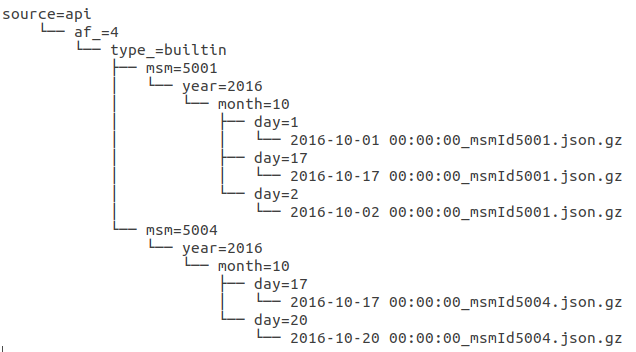
\includegraphics[width=1\linewidth]{illustrations/partitionnement-athena}
	\caption{L'organisation des traceroutes dans un compartiment Amazon S3}
	\label{fig:partitionnement-athena}
\end{figure}
 

\subsection{L'interrogation de données sur Amazon Athena}

L'interrogation de données présentes sur Amazon S3 via Amazon Athena est effectué avec une requête SQL. On peut décomposer une requête SQL en trois parties principales:
\paragraph{Les données sollicitées} Ça peut être une colonne ou bien bien une colonne transformée suite à l'application d'une ou de plusieurs fonctions de Presto.
\paragraph{Les partitions de données concernées} La requête SQL est paramétrée de sorte à limiter les données à analyser sur Amazon S3. 
\paragraph{Les paramètres appliqués sur les colonnes} La requête SQL doit filtrer les données suivant les conditions sur les colonnes de la table.

En pratique, nous avons créé la requête SQL reprise dans la Figure \ref{fig:sqlrequestathena}. 


Pour les données sollicitées, ce sont les trois colonnes \textit{prb\_id}, \textit{from}, \textit{msm\_id} (ligne $2$)et la liste de saut (\textit{hops})obtenue après quelques vérifications (lignes $3$ à $9$). A la ligne $10$, c'est la table créée pour les traceroutes (voir les détails de la table dans \ref{createAthenaTable}). Les traceroutes à analyser sont ceux obtenus en vérifiant les conditions dans la ligne  $12$ et $13$. C'est à dire, Athena va regarder les traceroutes qui se trouvent dans les sous dossiers year=2016\\month=10\\day=21 qui se trouvent aussi dans les deux dossiers msm=5001 et msm=5004. Ce que revient à chercher les traceroutes dans les deux endroits suivants:

\begin{lstlisting}[basicstyle= \footnotesize]
s3://ripeatlasdata/traceroute/source=api/af_=4/type_=builtin/msm=5001/year=2016/month=10/day=21

s3://ripeatlasdata/traceroute/source=api/af_=4/type_=builtin/msm=5004/year=2016/month=10/day=21
\end{lstlisting}



\begin{figure}[H]
	\centering
	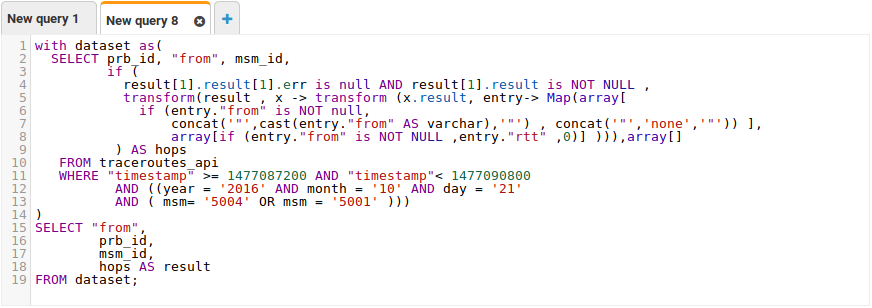
\includegraphics[width=1\linewidth]{illustrations/sqlRequestAthena.png}
	\caption{Une exemple d'une requête SQL sur Amazon Athena}
	\label{fig:sqlrequestathena}
\end{figure}



\include{annexe_machine}
\chapter{La détection d'anomalies en Scala} \label{application:spark}

%\subsection{Complément d'information du processus de la détection avec le langage Scala}
Comme complément aux étapes ($1$ à $9$) décrites dans la section \ref{steps-rtt-analysis}, on présente les différentes classes permettant de modéliser les données tout au long du processus de l'analyse. La définition de ces classes est effectuée en langage \textit{Scala}. 

Soient les classes suivantes utilisées : 

\paragraph{La classe Signal} modélise un signal \footnote{Un signal dans le contexte d'un traceroute.}. Ainsi, \textit{from} est l'adresse IP du routeur émettant ce signal, \textit{rtt} est le Round Trip Time entre la sonde Atlas et ce routeur et enfin \textit{x} est un indicateur de l'échec du signal.
\begin{lstlisting}[language=scala, caption={La classe Signal en Scala }]
case class Signal(
	rtt:  Option[Double],
	x:    Option[String],
	from: Option[String])

\end{lstlisting}

\paragraph{La classe Hop} modélise un saut dans un traceroute. On caractérise un saut par son identifiant noté \textit{hop}. Celui-ci   prend comme valeur un entier commençant à $1$ et la liste des signaux relatifs à ce saut, appelée  \textit{result}. Généralement un saut est représenté par $3$ signaux.
\begin{lstlisting}[language=scala, caption={La classe Hop en Scala }]
case class Hop(
	var result: Seq[Signal],
	hop:        Int)
\end{lstlisting}
\paragraph{La classe Traceroutes} modélise le résultat d'une requête traceroute effectuée par une sonde Atlas. Cette modélisation se limite aux données qui nous intéressent dans la présente analyse : 
\textit{dst\_name} représente l'adresse IP de la destination de la requête traceroute, \textit{from} est l'adresse IP de la sonde, \textit{prb\_id} est l'identifiant de la sonde, \textit{msm\_id} est l'identifiant de mesure, \textit{timestamp} est le temps auquel la requête traceroute a été effectuée et enfin on trouve la liste des sauts qui représentent les routeurs traversés par le trafic entre la source et la destination. 

\begin{lstlisting}[language=scala, caption={La classe Traceroute en Scala }]
case class Traceroute(
	dst_name:  String,
	from:      String,
	prb_id:    BigInt,
	msm_id:    BigInt,
	timestamp: BigInt,
	result:    Seq[Hop])
\end{lstlisting}
\paragraph{La classe TraceroutesPerPeriod} permet de présenter les traceroutes après les avoir regroupé    suivant la période pendant laquelle ils ont été effectués.   \textit{timeWindow} est le temps unix marquant le début de la période \footnote{Pour précision, la fin de la période peut être inférée en prenant deux débuts de deux périodes consécutives car la durée d'une période est fixe tout au long de l'analyse.} et  \textit{traceroutes} est la liste des traceroutes effectués pendant cette période. 


A l'étape 2, l'objectif était d'agréger  les signaux par routeur source et ensuite calculer la médiane des RTTs par ce routeur. Par conséquent, un traceroute est présenté différemment, ce qui est  illustré par la classe \textit{MedianByHopTraceroute}.

\paragraph{La classe PreparedSignal }  est une agrégation de tous les signaux, d'un saut donné, par le routeur \textit{from},  la médiane des RTTs calculée est présentée par \textit{medianRtt}.
\begin{lstlisting}[language=scala, caption={La classe PreparedSignal en Scala }]
case class PreparedSignal(
	medianRtt: Double,
	from:      String)
\end{lstlisting}
\paragraph{La classe PreparedHop } modélise un saut après avoir agrégé ses signaux. 
\begin{lstlisting}[language=scala, caption={La classe PreparedHop en Scala }]
case class PreparedHop(
	var result: Seq[PreparedSignal],
	hop:        Int)
\end{lstlisting}


\paragraph{La classe MedianByHopTraceroute } modélise un traceroute après avoir agrégé ses sauts. Par rapport au traceroute d'avant l'agrégation, seule la liste des sauts  a subi un changement. 
\begin{lstlisting}[language=scala, caption={La classe MedianByHopTraceroute en Scala }]
case class MedianByHopTraceroute(
	dst_name:  String,
	from:      String,
	prb_id:    BigInt,
	msm_id:    BigInt,
	timestamp: BigInt,
	result:    Seq[PreparedHop])
\end{lstlisting}


\paragraph{La classe Link} modélise un lien topologique. Ce dernier est défini par deux adresses IP  \textit{ip1} et \textit{ip2} et par son RTT différentiel calculé \textit{rttDiff}.
\begin{lstlisting}[language=scala, caption={La classe Link en Scala }]
case class Link(
	ip1:     String,
	ip2:     String,
	rttDiff: Double)
\end{lstlisting}

\paragraph{La classe LinksTraceroute} permet de modéliser un traceroute après avoir inféré tous ses liens. Ainsi, la liste des sauts est remplacée par la liste des liens (\textit{links}). 

\begin{lstlisting}[language=scala, caption={La classe LinksTraceroute en Scala }]
case class LinksTraceroute(
	dst_name:  String,
	from:      String,
	prb_id:    BigInt,
	msm_id:    BigInt,
	timestamp: BigInt,
	links:     Seq[Link])
\end{lstlisting}


A l'étape $5$, l'objectif est de passer d'un traceroute à une liste de liens caractérisés par les informations générales de la requête traceroute et leurs RTTs différentiels. Chaque élément de cette liste est représenté par la classe \textit{DiffRtt}, où \textit{LinkIPs} représente les deux adresses IP d'un lien donné.
\paragraph{La classe LinkIPs} permet représenter un lien par seulement ses deux adresses IP \textit{ip1} et \textit{ip2}.
\begin{lstlisting}[language=scala, caption={La classe LinkIPs en Scala }]
case class LinkIPs(
	ip1: String,
	ip2: String)
\end{lstlisting}

\paragraph{La classe DiffRtt} est une représentation plus détaillée d'un lien, en plus de son RTT différentiel, on ajoute d'autres informations.  Les adresses IP d'un lien sont modélisées par la classe \textit{LinkIPs}.

\begin{lstlisting}[language=scala, caption={La classe DiffRtt en Scala }]
case class DiffRtt(
	rtt:      Double,
	var link: LinkIPs,
	probe:    BigInt)
\end{lstlisting}

A l'étape $6.2$, on souhaite normaliser les dates de chaque lien; peu importe le moment pendant lequel le traceroute a été effectué durant une période $d_k$, on note seulement le début de cette période. Ainsi,  la classe  \textit{DiffRTTPeriod}  reprend un \textit{lien} donné, les différentes sondes Atlas ayant identifié ce lien (\textit{probes}), les RTTs différentiels de ce lien tout au long de cette période (\textit{rtts}) et enfin les dates associées à chaque RTT différentiel (\textit{dates}).
\paragraph{La classe DiffRTTPeriod } ~
\begin{lstlisting}[language=scala, caption={La classe DiffRTTPeriod en Scala }]
case class DiffRTTPeriod(
	link:      LinkIPs,
	probes:    Seq[BigInt],
	rtts:      Seq[Double],
	var dates: Seq[Int])
\end{lstlisting}

A la fin des opérations de l'étape $6$, on reprend pour chaque période, pour un lien donné, les RTTs différentiels ainsi que leurs dates. Ensuite, on calcule les bornes de l'intervalle de confiance courant pour ce lien et les bornes de l'intervalle de confiance de référence, et ce afin de comparer ces deux intervalles en vue d'inférer les anomalies possibles du délais de ce lien. Les intervalles de confiance sont calculés à en utilisant  la méthode des scores de Wilson.


\paragraph{La classe LinkState } permet de modéliser les intervalles de confiance d'un lien pendant une période $d_k$ donnée. \textit{valueLow} est la borne inférieur de l'intervalle de confiance, \textit{valueHi} est la borne supérieure de l'intervalle de confiance, \textit{valueMedian} est la médiane des RTTs différentiels et enfin \textit{valueMean} est la moyenne des RTTs différentiels. Pour précision, les données concernant l'état d'un lien sont sous forme d'une liste. L'idée est de garder l'historique de ces valeurs durant toute la période de l'analyse. Cette historique est exploitée pour tracer l'évolution du RTT différentiel du lien. Cependant, la comparaison utilise les valeurs du dernier état du lien.

  

%Pour toute période, on a une instance de \textit{LinkState} pour 
\begin{lstlisting}[language=scala, caption={La classe LinkState en Scala }]
case class LinkState(
	var valueMedian: Seq[Double],
	var valueHi:     Seq[Double],
	var valueLow:    Seq[Double],
	var valueMean:   Seq[Double])
\end{lstlisting}

Nous avons décrit les différentes classes utilisées. En ce qui concerne les traitements à appliquer sur les données, ce sont les fonctions permettant de répondre aux détails des étapes décrites dans la section  \ref{steps-rtt-analysis}.
\chapter{Les résultats de test de performances}

\section{MongoDB}
\begin{table}[H]
\captionsetup{justification=centering}
	\begin{tabular}{ccc}
	Période&Taille (GB)&Essai 1 \\ \hline
	07/02/18&1 &752,03 \\ \hline
	07/02/2018 – 08/02/2018& 2&$ 1499,28 $\\ \hline
	07/02/2018 – 09/02/2018&3&$ 2275,89 $\\ \hline
	07/02/2018 – 10/02/2018&4&$ 3035,19 $\\ \hline
	07/02/2018 – 11/02/2018&5&$ 3871 $\\ \hline
	\end{tabular}
    \caption{Les temps d'exécution d'analyse de traceroutes en fonction de la taille de données avec MongoDB}
    \label{tab:mongotiming-timing}
\end{table}


%\begin{table}[H]
%	%\begin{threeparttable}
%	
%	\captionsetup{justification=centering}
%	\begin{tabular}{ccccc}
%		\textbf{Début - fin} &\textbf{Durée (jours)}  & \textbf{Taille}  & \textbf{Nb traceroutes} & \textbf{Temps (secondes)} \\ \hline
%		
%		07/02/2018             &1 &1 GB&& 3870\\ \hline
%		07/02/2018 - 08/02/2018&2 &1 GB&& 2942\\ \hline
%		07/02/2018 - 09/02/2018&3 & 1 GB&& 2991\\ \hline
%		07/02/2018 - 10/02/2018&4 & 3 GB&& 20955\\ \hline
%		07/02/2018 - 11/02/2018&5& && \\ \hline
%		07/02/2018 - 12/02/2018&6& && \\ \hline
%		07/02/2018 - 13/02/2018&7& && \\ \hline
%		07/02/2018 - 14/02/2018&8& && \\ \hline
%	    07/02/2018 - 15/02/2018&9& && \\ \hline
%	    07/02/2018 - 16/02/2018&10& && \\ \hline
%	    07/02/2018 - 17/02/2018&11& && \\ \hline
%	    07/02/2018 - 18/02/2018&12& && \\ \hline
%	    07/02/2018 - 19/02/2018&13& && \\ \hline
%	    07/02/2018 - 20/02/2018&14& && \\ \hline
%	\end{tabular}
%	\caption{La moyenne des temps d'exécution d'analyse de traceroutes en fonction de la taille de données avec MongoDB}
%	\label{tab:mongotiming-timing}
%\end{table}
%\chapter{Notions et concepts}

\paragraph{In-memory}

\newpage
\listoffigures
\newpage
\listoftables
\newpage
\lstlistoflistings
\newpage
%\chapter{Application de quelques technologies Big Data sur l'analyse des  traceroutes} \label{chap:application-on-traceroutes}


\section{Introduction}

Ce chapitre reprend un ensemble de   technologies destinées  à la manipulation des données massives. Ce sont les technologies que nous avons expérimenté pour analyser des traceroutes disponibles dans le dépôt de RIPE Atlas. Précisément, ce sont les traceroutes permettant de tracer l'évolution du délai d'un lien comme c'est détaillé dans le chapitre \ref{chap:big-data-intro}.
% Nous allons présenter l'objectif de chaque technologie, ses avantages, ses inconvénients et ses limitations dans le cas de la présente analyse.
%Le présent chapitre reprend l'application de quelques technologies du Big Data manipulées en vue d'analyser le délai des liens. 
%On ne peut pas comparer ces technologies entre elles car elles ne se trouvent pas dans la même catégorie; quelques technologies n'assurent que le stockage, une autre technologie gère l'analyse ainsi que le stockage.  En revanche,
Les technologies que nous présentons  couvrent les besoins d'une ou de plusieurs étapes d'un processus d'analyse de données.
% (voir un exemple d'un processus d'analyse de données dans la section \ref{sec:process-data-analysis}). 
 
 %L'évaluation des performances  des technologies choisies est faite sur une machine ayant les caractéristiques reprises dans le tableau[!].

\section{Critères d'évaluation des technologies  Big Data}
Les critères d'évaluation d'une technologie Big Data  varient  suivant son objectif : stockage, calcul, etc.  En générale, la liste des critères que l'on peut considérer dans la comparaison des technologies Big Data est très longue.  Les critères sur lesquels nous  évaluons  les différentes technologies  Big Data expérimentées sont les suivants:
\begin{itemize}
	\item facilité de la mise en route et de la configuration de l'environnement de la technologie;
	\item flexibilité liée à la définition du  schéma de  données présentes dans les fichiers;
	\item temps d'exécution nécessaire pour fournir les résultats finaux d'une analyse de traceroutes;
	\item évolutivité de l'environnement Big Data mis en place pour des nouvelles données et de nouveaux besoins.
\end{itemize}

Dans la présente évaluation de quelques technologies Big Data, nous n'avons pas pris en compte d'autres critères. Car nous ne pouvons pas les évaluer. Par exemple, l'utilisation du  Big Data engendre des coûts  liés aux ressources nécessaires au stockage de données massives ainsi qu'au traitement de ces dernières. Nous avons donné des indications théoriques concernant les frais d'utilisation de deux technologies dédiées au stockage de données massives : Amazon S3 (voir le Tableau \ref{tab:pricing-s3-standard}) et MongoDB Atlas dont les frais d'utilisation  dépendent de plusieurs paramètres\footnote{Une estimation est possible suivant le fournisseur de cloud, elle est disponible  sur \url{https://www.mongodb.com/cloud/atlas/pricing}, consulté le $25/12/2018$.}. 

\section{Caractéristiques de l'environnement de test} \label{machine-openvz-caracteritics}

\paragraph{La machine de test} L'évaluation des technologies Big Data choisies sur un échantillon de traceroutes a été réalisé sur un conteneur de type OpenVZ ayant les caractéristiques suivantes :  système Debian GNU/Linux 7.11 (wheezy),  32,768 MB de  RAM, CPU MHz $ 2294.331 $.
%, nombre de CPUs $64$.

%Le Tableau \ref{tab:test-machine} présente les caractéristique de la machine sur laquelle nous avons effectué les différents tests. 
%\begin{table}[H]
%	\begin{tabular}{cc}
%		Type& OpenVZ container\\
%		RAM (MB)& 32768 \\
%		CPU & 64 (The logical CPU number of a CPU as used by the Linux kernel) \\
%	\end{tabular}
%	\caption{Caractéristiques de la machine de test}
%	\label{tab:test-machine}
%\end{table}
\begin{tcolorbox}
	Il existe différentes catégories de virtualisation. \textbf{OpenVZ} s'inscrit dans la catégorie Isolateur. Un isolateur est un logiciel permettant d'isoler l'exécution des applications dans des contextes ou zones d'exécution. Un conteneur OpenVZ  adopte un partitionnement logique au niveau des ressources systèmes : processus, réseau et système de fichier\footnote{Source : \url{http://cesar.resinfo.org/IMG/pdf/jtsiars-openvz_1_.pdf}, consultée le $29/12/2018$.}.
\end{tcolorbox}

Les différents tests effectués, présentés dans le présent chapitre, ont été effectués  au sein de cette machine. Nous notons qu'un seul test est lancé à un moment donné dans la machine.
\paragraph{Paramètres de l'analyse} Pour les paramètres de détection, nous avons utilisé les valeurs suivantes : \textit{timeWindow} est de $ 3600 $ secondes, l'intervalle de confiance est de $0,05$, \textit{alpha} est de $ 0,01 $ et \textit{minSeen} est de $3$. Les dates de début et de fin  varient suivant les traceroutes analysés.


\section{Collecte des traceroutes depuis le dépôt d'Atlas }
Nous avons utilisé l'API d'Atlas  comme source pour récupérer les traceroutes depuis le dépôt d'Atlas. L'API permet de collecter des traceroutes depuis le dépôt d'Atlas en ajustant quelques paramètres comme  l'identifiant de la mesure, la période souhaitée, etc. Toutefois, les données collectés doivent être réorganisées. Précisément, il faut passer d'un fichier d'une seule ligne qui contient une liste de traceroute à un fichier contenant plusieurs lignes et chaque ligne représente un traceroute. Nous avons manipulé des échantillons de traceroutes dont la taille entre $ 1 $ et $ 10 $ GO, ce sont des volumes  adaptés pour que la machine de test prenne en charge la récupération de ces volumes  et ensuite  réorganisation de ces traceroutes. 
La réorganisation des traceroute n'est pas nécessaire  MongoDB; l'import des traceroutes vers une base de données MongoDB peut être fait soit  via la liste des traceroutes ou bien via des lignes dans un fichier. Pour Amazon Athena et Spark, chaque traceroute doit occuper une  ligne dans les fichiers dans lesquels ils sont stockés. 

\section{Application 1 : MongoDB} \label{mongodb-impleme}
%\paragraph{ Application sur  MongoDB}~

%Les données relatives aux mesures traceroutes peuvent être récupérées de différentes manières. Par exemple,  les traceroutes à destination des instances du serveur DNS K-root. En ce qui concerne le travail de référence, les traceroutes sont récupérés à la fois par type d'adressage : IPv4 et IPv6 en se basant sur  l'identifiant  de la mesure : $ 5001 $, $ 6006 $, etc et par date.  Ainsi les

\paragraph{Evaluation des critères de sélection}~

MongoDB est la technologie Big Data utilisée par  Fontugne et al.  dans l'implémentation de l'outil de détection \cite{InternetHealthReport}. Dans MongoDB, les traceroutes sont organisés  dans des collections.  Chaque collection stocke les traceroutes effectués lors de la journée $YYYY\_MM\_DD$ et en adressage $V$. Par convention,  $V$  vaut $6$ s'il s'agit de l'adressage IPv6 et est vide.  La nomenclature  des collections permet de ne récupérer que les traceroutes concernés par l'analyse lancée. Le nom d'une collection est structuré comme suit: 	$tracerouteV\_YYYY\_MM\_DD$.
 

 
MongoDB est une technologie conçue pour assurer  le stockage de données dans un processus d'analyse de données. Nous avons utilisé la version locale de MongoDB, la quantité de données que nous pouvons stocker ainsi que le traitement appliqué sur les données récupérées dépendent principalement des ressources de la machine dans laquelle MongoDB est installé.
 
MongoDB est flexible en terme de définition du schéma de données; aucun schéma n'est requis.   Par exemple, dans certains cas, les traceroutes planifiés ne réussissent pas à atteindre une destination, dans ce cas, la structure de ces  traceroutes est différente  de la structure des traceroutes réussis. Les deux types de traceroutes sont stockés sans contrainte.

Les données stockées dans une collection MongoDB peuvent être manipulées en mode lecture et en mode écriture. Dans le premier, on cherche à lire des données en provenance de différentes sources. C'est le plus répandu dans les projets Big Data. Pour le deuxième mode, on peut mettre à jour un enregistrement dans une collection MongoDB. Ceci est moins fréquent dans les projets Big Data.

%Généralement l'analyse de données à grande échelle se limite qu'au mode lecture de données pour en tirer les connaissances. 
%MongoDB est adapté  aux projets visant la lecture de données massives mais aussi aux projets où on envisage la mise à jour d'un objet dans une collection (modification ou suppression). 
 
 MongoDB est évolutif; en cas de   mise à jour de la structure de nouveaux  objets traceroutes par Atlas,  cela n'affecte pas les données précédemment  stockées  dans MongoDB.
 
 %Malgré la convenance de MongoDB aux données non structurées et massives, l'utilisation de telle base de données, en version locale, nécessite l'ajustement de la machine locale où MongoDB tourne. 



%\paragraph{Les limitations de MongoDB}

%L'implémentation proposée de l'outil de détection utilise la version locale de la base de données MongoDB pour le stockage des données.  La quantité de données dont MongoDB peut stocker dépend de l'espace mémoire de stockage disponible dans la machine dans laquelle MongoDB est installé. De plus, les performances d'une détection lancée concernant une période donnée dépendent de la RAM de la machine en question. Pour conclure, l'utilisation de la version locale d MongoDB pour analyser les traceroutes à travers l'outil de détection dépend typiquement de la machine locale.
%\paragraph{Les performances de MongoDB}
\paragraph{Performances de la base de données MongoDB dans l'analyse des délais }~


Nous mesurons le temps écoulé durant l'analyse des traceroutes, stockés dans une base de données MongoDB,  en vue de détecter les anomalies dans le délai des liens. C'est le temps nécessaire à l'accomplissement des étapes de la phase I, de la phase II et de l'écriture des résultats dans un fichier. Chaque ligne de ce dernier  décrit un lien comme l'exemple donné dans le Listing \ref{resultLink}.  

Dans le Tableau \ref{tab:mongotiming-timing}, nous varions l'ensemble de traceroutes. Pour Chaque période, nous mesurons le temps nécessaire pour analyser les traceroutes capturés durant cette période pour plusieurs reprises. L'analyse de chaque période est fait $5$ fois, ce qu'on appelle ici des essais : Essai 1, Essai 2, etc.  Les traceroutes analysés sont ceux à destination des instances du f.root-servers.net\footnote{Voir les détails de la mesure 5004 sur \url{https://atlas.ripe.net/measurements/5004/}, consultée le $12/12/2018$}.

%en terme de stockage pour mesurer le temps nécessaire pour avoir  l'évolution de tous les liens présents dans  les traceroutes analysés, nous ne présentons que les premier trois essais. 


\begin{table}[h]
	\captionsetup{justification=centering}
	\resizebox{1\textwidth}{!}{
	\begin{tabular}{cccccccc}
\textbf{Période}&\textbf{Taille (bytes)}&\textbf{Essai 1 (s)}&\textbf{Essai 2 (s)} &\textbf{Essai 3 (s)}&\textbf{Essai 4 (s)}&\textbf{Essai 5 (s)}&\textbf{Médiane (s)} \\ \hline
$ 07/02/18 - 07/02/18 $&$  1,028,343,572 $&$  $&$  $&$  $ &&&\\ \hline 
$ 07/02/2018 - 08/02/2018 $&$  $&$  $&$  $&$  $ &&&\\ \hline 
$ 07/02/2018 - 09/02/2018 $&$  $&$  $&$  $&$  $ &&&\\ \hline 
$ 07/02/2018 - 10/02/2018 $&$  $&$  $&$  $&$  $&&&\\ \hline 
$ 07/02/2018 - 11/02/2018 $&$  $&$  $&$  $&$  $&&&  \\ \hline 
	\end{tabular}
}
\caption{Les temps d'exécution d'analyse de traceroutes en fonction de la taille de données avec MongoDB}
\label{tab:mongotiming-timing}
\end{table}

Nous reprenons les informations du Tableau \ref{tab:mongotiming-timing} dans la Figure \ref{fig:mongodbtiming}. L'axe  des abscisses représente la taille des fichiers contenant les traceroutes  analysés, appelée  $q$. L'axe  des ordonnées  représente le temps nécessaire à l'analyse d'une quantité  de traceroutes. Nous agrégeons les temps des différents essais et nous calculons  leur valeur minimale, maximale et la médiane.
Pour précision, le temps calculé est la différence entre l'instant  qui précède le lancement de l'analyse et l'instant qui suit la fin de l'analyse.

\begin{figure}[h]
	\centering
	\captionsetup{justification=centering}
	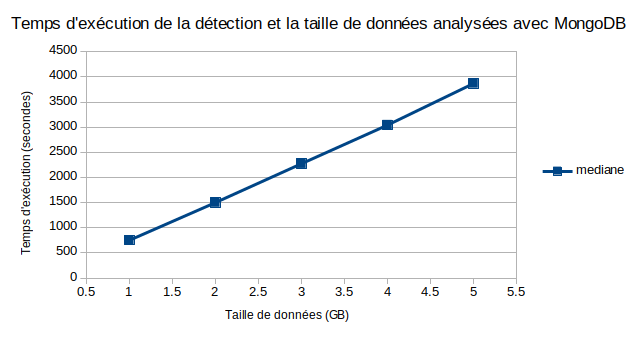
\includegraphics[width=0.7\linewidth]{illustrations/mongoDBtiming_0}
	\caption{}
	\label{fig:mongodbtiming}
\end{figure}

%Tandis que la  Figure \ref{fig:mongodbtiming}	 reprend la médiane  des temps d'exécution de la détection en fonction de  la taille de données analysées en utilisant MongoDB. 
%La Figure 	 \ref{fig:moustachemongodb} illustre la variation de la distribution des temps d'exécution. La Figure 	 \ref{fig:moustachemongodb} ainsi que la Figure \ref{fig:mongodbtiming} ont été obtenues en considérant les temps d'exécution de $10$ essais pour chaque taille de données.




%\begin{figure}[h]
%	\centering
%		\captionsetup{justification=centering}
%	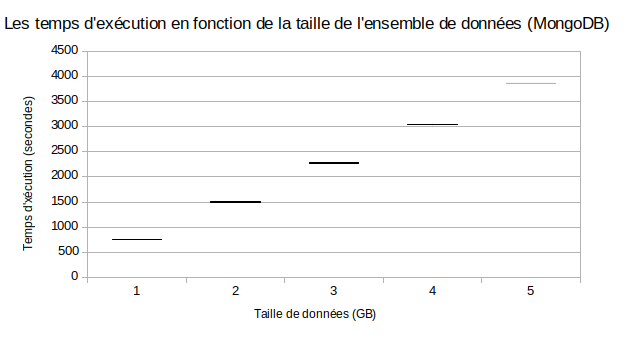
\includegraphics[width=0.7\linewidth]{illustrations/moustacheMongodb_0}
%	\caption{Les temps d'exécution en fonction de la taille de traceroutes analysés (MongoDB)}
%	\label{fig:moustachemongodb}
%\end{figure}

%La variation des temps d'exécution en fonction du nombre de traceroutes 


%Nous évaluons les temps d'exécution lors de l'analyse des délais des liens présents dans un ensemble de traceroutes, en utilisant MongoDB comme technologie de stockage de données massives.   

%On distingue deux types de variations : la taille de l'ensemble de données en terme de stockage et la taille en nombre de traceroutes présents dans l'ensemble de données.

%\begin{table}[h]
%	\captionsetup{justification=centering}
%	\resizebox{1\textwidth}{!}{
%		\begin{tabular}{cccccccc}
%			\textbf{Période}&\textbf{Taille (bytes)}&\textbf{Essai 1 (s)}&\textbf{Essai 2 (s)} %&\textbf{Essai 3 (s)}&\textbf{Essai 4 (s)}&\textbf{Essai 5 (s)}&\textbf{Médiane (s)} \\ %\hline
%			$ 07/02/18 - 07/02/18 $&$  1,028,343,572 $&$ 752,03 $&$ 750 $&$ 755,24 $ &&&\\ \hline 
%			$ 07/02/2018 - 08/02/2018 $&$ 2 $&$ 1499,28 $&$ 1504,98 $&$ 1503,62 $ &&&\\ \hline 
%			$ 07/02/2018 - 09/02/2018 $&$ 3 $&$ 2275,89 $&$2265,96 $&$ 2284,98 $ &&&\\ \hline 
%			$ 07/02/2018 - 10/02/2018 $&$ 4 $&$ 3035,19 $&$ 3043,21 $&$ 3057,45 $&&&\\ \hline 
%			$ 07/02/2018 - 11/02/2018 $&$ 5 $&$ 3871 $&$ 3889,57 $&$ 3894,5 $&&&  \\ \hline 
%		\end{tabular}
%	}
\section{Application 2 : Amazon DynamoDB}


%\paragraph{Application sur les traceroutes}~


L'élasticité est une des caractéristiques attirantes des services web d'Amazon. En particulier, c'est le cas d'Amazon DynamoDB. Ainsi, une implémentation basée sur Amazon DynamoDB  n'a pas à se soucier de la capacité  de stockage de données si la quantité de données évolue rapidement. 

 Amazon DynamoDB  n'assure que le stockage de données dans un processus d'analyse de données. La récupération et le traitement  des données stockées nécessitent l'ajustement des ressources de la machine qui reçoivent ces données, pareillement à MongoDB. La différence se situe à l'évolutivité implicite du stockage de données, qui ne se limite que par la capacité de stockage physique d'AWS. Tandis qu'une installation locale de MongoDB est liée aux ressources de la machine hébergeant ce dernier.  Nous n'avons pas expérimenté Amazon DynamoDB pour analyser les traceroutes, étant donné que notre évaluation des temps d'exécution est effectuée sur une machine locale, nous aurons les mêmes remarques que dans le cas de MongoDB en ce qui concerne l'ajustement des ressources de la machine qui reçoive les données.  
 
 A titre indicatif, une heure de tous les traceroutes effectués par toutes les sondes Atlas, concernant tous les identifiants de mesure,  fait une taille moyenne de  $620$ MB en format compressé, ce que représente une quantité d'environ $9$ GB en format texte.
%Toutefois,  au moment de de la récupération et de la manipulation de ces données, il faut ajuster les ressources pour pouvoir récupérer et traiter une quantité importante de données.

\section{Application 3 : Amazon S3, Amazon Glue  et Amazon Athena }

%\paragraph{Application sur les traceroutes}~
\paragraph{Vue générale}~

Nous avons combiné les trois services d'Amazon (Amazon S3, Amazon Glue  et Amazon Athena)  afin de créer un environnement d'analyse de données massives. 
Un des scénarios possibles mettant en pratique ensemble ces trois services est illustré dans la Figure
\ref{fig:gluecrawler}\footnote{Amazon Redshift  est un entrepôt de données et  Amazon Quicksight  est un service cloud d'informatique décisionnelle.}. Nous détaillons chaque services dans les sections suivantes.

Afin d'utiliser Amazon Athena pour l'interrogations des traceroutes stockés dans des fichiers, nous avons besoin d'abord de stocker les fichiers dans Amazon S3. De plus, nous avons besoin de créer un  schéma de données. Il s'agit de créer une table comme les tables dans un SGBDR. Chaque enregistrement dans cette table correspond à une ligne dans les fichiers de données censés être lus par cette table. Il existe deux manières pour créer une table dans Athena : en utilisant Amazon Glue ou création manuelle. \textit{traceroutes\_api} désigne le nom de la table reprenant tous les traceroutes.
%Une vue globale du  processus de l'analyse  est illustré dans la Figure  

\begin{figure}[h]
	\centering
	\captionsetup{justification=centering}
	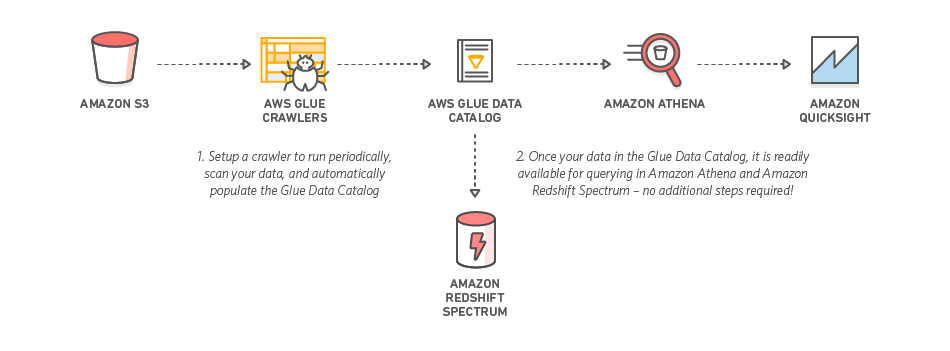
\includegraphics[width=1\linewidth]{illustrations/glue_crawler}
	\caption{Une combinaison des services web d'Amazon : Amazon S3, Amazon Glue, Amazon Athena, Amazon Quicksight  et Amazon Redshift}
	\label{fig:gluecrawler}
	\source{\url{https://docs.aws.amazon.com/fr_fr/athena/latest/ug/glue-best-practices.html}, consultée le $16/05/2018$.}
\end{figure}


\paragraph{Création de la table traceroutes avec Amazon Glue}~

Nous avons lancé    la détection automatique du schéma, avec Amazon Glue, d'un ensemble de  traceroutes enregistrés dans un fichier faisant une taille de $500$ MB. Toutefois, la détection a échoué. Autrement dit, Amazon Glue n'a pas pu inférer le schéma d'une seule table capable de lire tout traceroute dans ce fichier.  L'échec de l'inférence est dû au fait que le fichier contient des traceroutes différents en terme de structure, car la structure dépend de la version du firmware de la sonde ayant effectué le traceroute. Les différentes versions du firmware  pour chaque type de mesure sont détaillées dans le site Web d'Atlas\footnote{\url{https://atlas.ripe.net/docs/data_struct/}, consultée le $16/01/2018$.}.
 %L'origine de cette différence  est le fait que ces traceroutes ont été effectués par des sondes ayant un firmware différent. Car le contenu des résultats d'une requête traceroute  et son organisation dans un objet JSON dépend partiellement du firmware de la sonde. 
 
\paragraph{Création manuelle de la table \textit{traceroutes\_api}}~

Nous avons créé la structure de la table \textit{traceroutes\_api}  manuellement en se basant sur la structure détaillée d'une réponse traceroute pour chaque version du firmware. Les différentes structures de réponses d'une requête traceroute n'a posé aucun problème dans la création manuelle de la table. Dans notre cas, la réussite de la création manuelle est due au fait que les attributs dont l'outil de détection a besoin sont présents dans toutes les versions du firmware d'une part. D'autre part, Amazon Athena est flexible en ce qui concerne l'association entre un objet JSON et un enregistrement dans une table. Autrement dit, si un attribut existe dans l'objet JSON, la colonne correspondante prend sa valeur et vide dans le cas échéant.  

\paragraph{Partitionnement des données stockés dans Amazon S3}~

Nous avons   pris en compte  le partitionnement de données dans un compartiment S3 dans la création de la table \textit{traceroutes\_api}.  L'utilisation du partitionnement est optionnel. 
Le partitionnement  de données présentes dans un compartiment Amazon S3 permet de limiter la quantité de données à analyser par une requête Amazon Athena. Le partitionnement améliore  les performances d'Amazon Athena. D'une part, la requête s'exécute rapidement. D'autre part, le partitionnement réduit les coûts engendrés  suite à l'utilisation d'Amazon Athena, car ce dernier est facturé selon la quantité de données analysées. En pratique,  une partition créée joue un rôle similaire à celui d'une colonne durant l'interrogation d'une table dans Athena. 

Prenons un exemple illustrant l'apport du partitionnement. Nous avons des traceroutes effectué en adressage IP la version  $ 4 $ et $ 6 $.


\textit{af\_} désigne le type d'adressage : \textit{af\_} vaut $4$ en cas d'adressage IPv4 et $6$ en cas d'adressage IPv6. Sans l'utilisation du partitionnement et si on ne souhaite récupérer que  les traceroutes ayant comme adressage IPv4, tous les traceroutes présents dans le compartiment S3 (appelé \textit{s3://ripeatlasdata}), dédié au stockage des traceroutes récupérés depuis le dépôt d'Atlas, sont évalués\footnote{L'évaluation du type  d'adressage est effectué selon la valeur de l'attribut \textit{af} d'un traceroute, il vaut \textit{4} ou \textit{6}.}.

Toutefois, en partitionnant les données suivant par exemple le type d'adressage, seuls les fichiers dans la partition\footnote{Partition dans le sens d'Amazon Athena.} af\_ = 4 qui sont analysés. Par conséquent, le partitionnement permet de réduire les coûts d'utilisation du service Amazon Athena, surtout si la quantité de données est très importante. 


Les partitions   créées sont illustrées  dans la Figure 	\ref{fig:partitionnement-athenaa}. Nous détaillons les différentes partitions dans le Tableau \ref{tab:partition-description}. Nous donnons le nom de la partition dans la première colonne, quelques valeurs de chaque partition dans la deuxième colonne et la troisième colonne de ce tableau reprend une description de la partition.

\begin{figure}[H]
	\centering
	\captionsetup{justification=centering}
	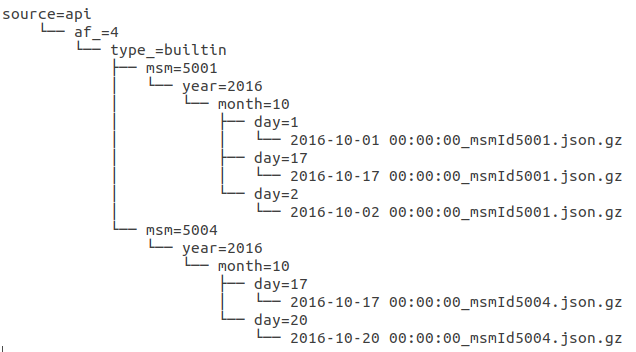
\includegraphics[width=1\linewidth]{illustrations/partitionnement-athena}
	\caption{L'organisation des traceroutes dans le compartiment Amazon S3 \textit{s3://ripeatlasdata}}
	\label{fig:partitionnement-athenaa}
\end{figure}

\begin{table}
		\centering
		\captionsetup{justification=centering}
\begin{tabular}{|c|c|l|}
	\hline 
\textbf{partition}	& \textbf{Valeurs} & \multicolumn{1}{c|}{\textbf{Commentaires} }\\ 
	\hline 
 source& api & Les  traceroutes récupérés depuis le dépôt  d'Atlas via l'API \\ 
	\cline{2-3}
	 &typeanddate& Les  traceroutes récupérés depuis la page Web\\
	\hline 
	af\_& 4  & Les traceroutes en adressage IPv4 \\ 
	\cline{2-3} &6& Les traceroutes en adressage IPv6\\	\hline 
	type& builtin  & Les traceroutes en provenances des mesures intégrées \\ 
	\cline{2-3} 
 &anchor& Les traceroutes à destinations des ancres\\ \hline
	msm& 5001 & Les traceroutes ayant msm\_id = 5001 \\ 
	\cline{2-3}  &5004& Les traceroutes ayant msm\_id = 5001 \\
	\hline 
	year& 2016 & Les traceroutes effectués en $2016$ \\ 
	\hline 
	month& 10 & Les traceroutes effectués en octobre \\ 
	\hline 
	day& 1 & Les traceroutes effectué le premier du mois \\ 
	\hline 
\end{tabular}
\caption{Exemple des partitions créées dans un compartiment Amazon S3} 
\label{tab:partition-description}
\end{table}

 Les   partitions \textit{af\_} et \textit{type\_} sont nommée de cette manière, au lieu de \textit{af} et \textit{type} car  la table \textit{traceroutes\_api} contient des colonnes avec ces noms et comme les partitions agissent comme des colonnes  lors de l'évaluation d'une requêtes avec Amazon Athena, les noms de ces partitions ont été adaptés.

Par exemple, les traceroutes qui se trouvent dans  le fichier

 \textit{2016-10-01 00:00:00\_msmId5001.json.gz} sont analysés par toute requête Athena  
impliquant les partitions d'une des manières suivantes : 
(source = api) ou (source = api et af\_ = 4) ou (source = api et af\_ = 4 et type = builtin) ou (source = api et af\_ = 4 et type = builtin et msm = 5001) ou 
(source = api et af\_ = 4 et type = builtin et msm = 5001 et year = 2016) ou (source = api et af\_ = 4 et type = builtin et msm = 5001 et year = 2016 et month = 10) ou
 (source = api et af\_ = 4 et type = builtin et msm = 5001 et year = 2016 et month = 10 et day = 1).

\paragraph{Interrogation des données Avec Amazon Athena}~

Une fois les fichiers de données  synchronisés vers le compartiment AWS S3 et le schéma  de données  créé, on passe à l'interrogation de données en utilisant les requêtes SQL basées sur Presto.  
Nous donnons un exemple d'une requête Athena dans la section \ref{sql-athena-request} de l'annexe \ref{athena-appendix}.

\paragraph{Intégration d'Amazon Athena dans l'outil de détection}~ \label{integration-aws-possibilite-une}
 

Pour intégrer Amazon Athena dans l'outil de détection \cite{InternetHealthReport}, on distingue deux possibilités. La première possibilité n'utilise Athena que pour récupérer  les traceroutes stockés dans Amazon S3 vers  la machine locale. Ensuite, cette dernière poursuit les traitements  décrits dans la phase I et II. Dans ce cas, nous ne profitons pas  des performances d'Amazon Athena vu que les traitements complexes sont effectués dans la machine locale.
%vérifiés en terme de validité; c'est l'objectif des étapes $1$ et $2$ dans le processus de la création de l'évolution des RTTs différentiels des liens (voir la section \ref{steps-rtt-analysis}).  
 %Les traitements qui suivent (étapes  à partir de $3$) sont effectués dans la machine locale. Dans ce cas, l'utilisation des technologies  Big Data est limité qu'au niveau stockage de données massives. 

Tandis que  la deuxième possibilité vise la maximisation des traitements des deux phases I et II au sein de l'infrastructure  d'Athena. De ce fait, la machine locale n'a qu'à recevoir les derniers résultats de la détection, voire les résultats finaux. Pour cette deuxième possibilité, les données doivent être manipulées de sorte à maximiser,  	au niveau d'Amazon Athena,  les traitements relatifs à toutes les étapes des deux phases I et II. 

Pour la deuxième possibilité, le défi est de trouver la requête ou bien l'ensemble de requêtes SQL à exécuter sur Athena en vue d'avoir l'évolution du RTT différentiel des liens. 
Vu la complexité des  étapes des phases I et II, on ne peut pas trouver une seule requête SQL assurant toutes ces étapes à la fois. Supposons qu'il existe une requête SQL capable de trouver les liens possibles avec leurs RTTs différentiels : à l'étape $ 4 $ dans \ref{steps-rtt-analysis}, on construit la distribution des RTTs différentiels pour tout lien $l$ identifié dans les traceroutes de la période $d_k$. Cette distribution est mise à jour à chaque fois $l$ est identifié dans un des traceroutes  de la période $d_k$. 

Soient  $T_k$ = \{$t_{k, j}$\}  l'ensemble de traceroutes effectués durant $d_k$, avec $j \in [1, R_k]$ et $R_k$ est le nombre de traceroutes effectués durant $d_k$. Nous décrivons le parcours des traceroutes d'une période $d_k$ brièvement dans le pseudo-code \ref{alo-inference-link}. Nous n'avons pas donné  tous les détails, car l'objectif est d'évaluer la convenance d'Athena au traitement souhaité.
\begin{algorithm}[H]
\begin{algorithmic}[1]
	 \ForAll{ $t_{k, j}$ $\in$ $T_k$} \
	  \State $links$ $\leftarrow$ getLinksFromTraceroute($t_{k, j}$)
	  	 \ForAll{$l$ $\in$ $links$}
	  	 		\State updateLinkRttDistribution($l$) \label{update-link}
	  	 \EndFor
	 \EndFor
\end{algorithmic}
\caption{Une partie de l'étape $4$ du processus de la détection des anomalies des délais }
\label{alo-inference-link}
\end{algorithm}

Avec : 
\begin{itemize}
	\item \textit{getLinksFromTraceroute($t_{k, j}$)} énumère tous les liens possibles dans le traceroute $t_{k, j}$.

    \item \textit{updateLinkRttDistribution($l$)} ajoute le RTT différentiel calculé du lien $l$ à la distribution des RTTs différentiels courante de ce lien pour la période $d_k$.
\end{itemize}


Le service Athena est conçu pour la lecture de données, toute mise à jour de données n'est pas possible avec ce service. C'est pourquoi la distribution des RTTs différentiels de chaque  lien identifié doit être sauvegardée dans un endroit accessible en lecture et en écriture, par exemple dans un compartiment AWS S3. Que ce soit un fichier reprenant la distribution des RTTs différentiels  par un seul lien ou bien un fichier pour tous les liens,   à la ligne  \ref{update-link} du pseudo-code \ref{alo-inference-link}, un fichier doit être lu et mise à jour avec de nouvelle valeur. Pour une période $d_k$ d'une heure, le nombre de traceroutes est de l'ordre de milliers. Chaque traceroute $t_{k,j}$ peut inclure $L_{k,j}$ liens. Dans ce cas, le nombre total, d'une période $d_k$, de mise à jour de la distribution des RTTs différentiels est    $ \sum_{m=1}^{R_k}  L_{k,m}$. $ L_{k,j} $ dépend du nombre de saut du  traceroute $t_{k,j}$.

 %de l'ordre $R_k$\texttimes$L$ de fois.  Cette estimation est à titre indicatif, de plus elle ne concerne que l'étape $4$, le nombre de lectures et/ou d'écritures dépend des requêtes SQL créées pour les autres étapes. 

En plus du nombre de lectures et d'écritures, relatives à la phase I, que nous venons de décrire, à la phase II, la détection des anomalies s'effectue en  comparant les intervalles de confiances : un intervalle de confiance courant du lien avec celui de référence. Cette comparaison révèle deux contraintes. La première contrainte concerne  la fonction permettant de calculer les deux bornes de l'intervalle de confiance de Wilson ne fait pas partie des fonctions disponibles sur Amazon Athena. D'autre part, Amazon Athena ne permet pas la création des fonctions personnalisées pour répondre à des besoins non couverts par Amazon Athena. La deuxième contrainte concerne la mise à jour de l'intervalle de confiance de référence qui doit être faite à chaque nouvelle période.


\paragraph{Evaluation des critères pour Amazon S3 et Amazon Athena  }~

Afin d'utiliser le service Amazon Athena à moindre coût, il est conseillé d'utiliser le partitionnement, car moins de frais sont appliqués. Si un partitionnement particulier est adopté, la création du schéma de données est basé sur ce partitionnement ainsi que les requêtes SQL destinés à l'interrogation de la table de données.

En ce qui concerne l'évolutivité d'une application basée sur ces deux services d'Amazon, on note que toute mise à jour de la structure de données des objets traceroutes peut affecter l'entièreté de la configuration initiale. A savoir, l'organisation des fichiers de données via le partitionnement, le schéma de données et les requêtes SQL.

 Quant à la flexibilité du schéma de données, le service  Amazon Athena est tolérant au données manquantes. Etant donné que la structure d'un objet traceroute dépend de la version du firmware de la sonde, nous avons créé trois schémas de tables. La première table  modélise tout objet traceroute de  version $5$, la deuxième modélise tout objet traceroute de version $6$ et enfin la troisième table modélise ceux ayant la version $7$. En expérimentant différentes requêtes, nous avons conclu  que Amazon Athena a pu récupérer les données de la version récente ($7$) via le schéma de la version $5$ malgré que la version $7$ a plus d'attributs par rapport à la version $5$.
 
%Avec une autre technologie qui travaille en mémoire, les résultats sont données plus rapidement. 

\paragraph{Performances des services Amazon S3 et Athena dans l'analyse des délais }~ \label{aws-perforsm}

Nous avons utilisé Amazon Athena et Amazon S3 pour analyser les traceroutes et détecter les anomalies des délais. Nous précisons que nous avons évalué la première possibilité décrite dans la section \ref{integration-aws-possibilite-une}. Nous avons bénéficié de la  possibilité  de lancer des requêtes destinées à Amazon Athena à travers l'API REST, précisément en Python. Et comme l'implémentation proposée par les auteurs du travail de référence est écrite en Python, nous avons adapté cette implémentation de sorte  de récupérer les traceroutes depuis   depuis Amazon S3 via Amazon Athena au   lieu de le faire depuis la base de données locale MongoDB.  

Etant donné que nous avons utilisé le partitionnement de données, une analyse des délais nécessite d'autres paramètres à ajuster en plus de ceux relatifs à la détection. Ce sont les paramètres permettant de sélectionner les traceroutes présents sur Amazon S3. Du fait que le partitionnement de données (voir une partie de l'arborescence dans la Figure 	\ref{fig:partitionnement-athena}) est réalisé sur base du type de traceroute (\textit{builtin} ou \textit{anchor}) et de l'identifiant de la mesure ($ 5004 $, $6001$, etc) qui a enregistré un traceroute, nous devons personnaliser  la requête visant la   récupération des traceroutes  depuis Amazon S3 pour qu'elle prennent en compte aussi les partitions.

Le Tableau \ref{tab:athena-data} contient les temps d'exécution suivant la taille de l'ensemble de données donné en entrée de la détection.

\begin{table}[H]
	\centering
	\captionsetup{justification=centering}
\begin{tabular}{c c c}
	\textbf{Période} & \textbf{Taille(GB)} & \textbf{Temps (secondes) } \\ 	\hline 
$ 07/02/18 - 07/02/18 $	&$ 1 $&	$ 1898.31 $ \\ 	\hline 
$ 07/02/2018 - 08/02/2018 $	&$ 2 $&	$ 3533.6562171 $ \\ 	\hline 
$ 07/02/2018 - 09/02/2018 $&	$ 3 $&	$ 5284.91494989  $ \\ 	\hline 
$ 07/02/2018 - 10/02/2018 $	&$ 4 $&$ 	7228.88 $  \\ 	\hline 
$ 07/02/2018 - 11/02/2018 $	&$ 5 $& $ 8984.873281	 $ \\ 	\hline 
\end{tabular} 
\caption{Les temps d'exécution par taille de l'ensemble de données (Amazon Athena et Amazon S3)}
\label{tab:athena-data}
\end{table}

Nous distinguons trois phases dans cette approche (approche 1). Premièrement,  les données sont récupérées depuis Amazon S3. Plusieurs facteurs affectent cette étapes, par exemple,  les conditions du réseau, les ressources allouées par Amazon pour répondre à chaque requête  Athena à destination des données disponibles sur Amazon S3, l'optimalité de la requête SQL, etc.  En deuxième lieu, les résultats de la requête doivent être désérialisés pour pouvoir les utiliser localement. Enfin, sur base des données récupérées, la détection des anomalies peut être déclenchée.
%
%
%Nous évaluons les temps d'exécution de plusieurs  analyses de délais lancées en variant la taille de données. Rappelons qu'il s'agit de la première possibilité: Amazon S3 pour le stockage de traceroutes et Amazon Athena pour récupérer les traceroutes valides, le reste de traitements sont effectués au sein de la machine locale.  Le Tableau	\ref{tab:awstiming-timing} reprend plus de détails. 
%\begin{table}[H]
%	%\begin{threeparttable}
%	
%	\captionsetup{justification=centering}
%	\begin{tabular}{ccccc}
%		\textbf{Début - fin} &\textbf{Durée (jours)}  & \textbf{Taille}  & \textbf{Nb traceroutes} & \textbf{Temps (secondes)} \\ \hline
%		
%		07/02/2018             &1 &1 GB&& 3870\\ \hline
%		07/02/2018 - 08/02/2018&2 &1 GB&& 2942\\ \hline
%		07/02/2018 - 09/02/2018&3 & 1 GB&& 2991\\ \hline
%		07/02/2018 - 10/02/2018&4 & 3 GB&& 20955\\ \hline
%		07/02/2018 - 11/02/2018&5& && \\ \hline
%		07/02/2018 - 12/02/2018&6& && \\ \hline
%		07/02/2018 - 13/02/2018&7& && \\ \hline
%		07/02/2018 - 14/02/2018&8& && \\ \hline
%		07/02/2018 - 15/02/2018&9& && \\ \hline
%		07/02/2018 - 16/02/2018&10& && \\ \hline
%		07/02/2018 - 17/02/2018&11& && \\ \hline
%		07/02/2018 - 18/02/2018&12& && \\ \hline
%		07/02/2018 - 19/02/2018&13& && \\ \hline
%		07/02/2018 - 20/02/2018&14& && \\ \hline
%	\end{tabular}
%	\caption{La moyenne des temps d'exécution d'analyse de traceroutes en fonction de la taille de données avec Amazon S3 et Amazon Athena }
%	\label{tab:awstiming-timing}
%\end{table}
La Figure \ref{fig:temps-avec-aws} présente un seul essai pour chacune des tailles utilisées auparavant avec MongoDB.  Le temps de chaque essai comprend l'étape de la récupération des traceroutes depuis Amazon S3, le temps de préparation des traceroute et enfin le temps de la détection des anomalies. Autrement dit, le temps nécessaire à la réalisation des phases I, II et celui nécessaire pour sauvegarder les résultats par lien.

\begin{figure}[H]
	\centering
	\captionsetup{justification=centering}
	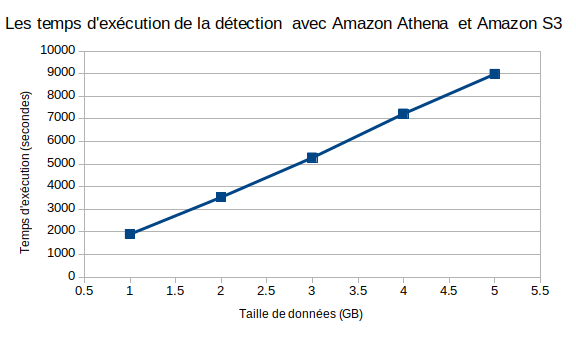
\includegraphics[width=0.7\linewidth]{illustrations/temps-avec-aws_1}
	\caption{Les temps d'exécution de la détection des anomalies en fonction de la taille de données (Amazon S3 et Amazon Athena)}
	\label{fig:temps-avec-aws}
\end{figure}


\section{Application 4 : Spark Apache avec Scala}
Nous avons implémenté l'outil de détection avec le framework Spark et l'API Scala. Les détails de l'implémentation sont donnés dans le chapitre \ref{application:spark}.  Nous avons évalué le temps d'exécution de l'outil de détection en analysant différents échantillons de traceroutes  en mode local et en mode cluster. Pour le mode local, nous avons lancer l'application Spark sur la machine ayant les caractéristiques  reprises dans la section \ref{machine-openvz-caracteritics}. Pour le mode cluster, nous avons utilisé le cluster EMR.


\subsection{Mode local}

A la base Spark est conçu pour être utilisé dans un cluster de machines sur  lequel l'analyse de données est distribuée. Toutefois, Spark peut être utilisé en mode local. Dans ce mode, on trouve le \textit{driver} et un seul \textit{executor}. Ce dernier est "lié" au même processus initié par le \textit{driver}. 


%\paragraph{Performances d'Apache Spark dans l'analyse des délais }~
Nous avons évalué le temps d'exécution de l'implémentation de l'outil de détection en utilisant Spark en variant le nombre de traceroutes à analyser. Nous avons aussi varié certains paramètres relatifs à la soumission de l'application au Spark. Nous avons varié la taille de la mémoire allouée au driver afin de choisir celle la plus adaptée. Ensuite nous avons mesuré le temps d'exécution dans le cas de local, local[K] et local[*].

\paragraph{Variant la mémoire allouée au driver}~

Dans une application Spark, la taille de la mémoire allouée pour le \textit{driver} et les \textit{executors} est  définie par défaut. D'après la documentation officielle de Spark\footnote{Source : \url{https://spark.apache.org/docs/latest/configuration.html}, consultée le $29/12/2018$.}, Spark réserve $ 1 $ GB pour le $ driver $ et $ 1 $ GB pour chaque \textit{executor}. 

En mode local (--master local), le \textit{driver} et le \textit{worker} sont liés au même processus.  Nous avons mesuré le temps d'exécution de l'application Spark en varaint la taille mémoire allouée au \textit{driver} via le paramètre \textit{driver-memory}. Par défaut, la mémoire allouée au driver est de 1 Go. Avec cette valeur, il n'est pas possible  d'analyser un ensemble de traceroutes qui fait $ 1,028,343,572 $ octets. Afin de voir l'effet de la mémoire allouée au \textit{driver}, en mode d'exécution local, nous avons utilisé deux échantillons de traceroutes. La première comprend les traceroutes capturés pendant le $ 07/02/2018 $ dans le cadre de la mesure ayant l'identifiant $ 5004 $, ce qui fait $ 1,028,343,572 $ octets (\textit{data\_1go}). Pour le deuxième échantillon, il reprend les traceroutes effectués  entre le $ 07/02/2018 $ et le $ 08/02/2018 $ effectués aussi dans le cadre de la mesure ayant l'identifiant $ 5004 $, ce qui fait $ 2,055,167,238 $ (\textit{ data\_2go}) octets.

La Figure 	\ref{fig:variantdrivermemory} présente les résultats obtenus. L'axe des abscisses indique la quantité de mémoire allouée au \textit{driver} et l'axe des ordonnées représente le temps d'exécution de détection. Pour les mêmes quantités de mémoire allouée au \textit{driver}, nous mesurons le temps d'exécution une fois pour  \textit{data\_1g}  et une autre fois pour  \textit{data\_2g}.
Pour les valeurs nulles relatives au temps d'exécution, l'exécution de la l'application a échoué. La raison de l'échec revient au manque de mémoire (message d'erreur est OutOfMemoryError: Java heap space).
\begin{figure}[H]
	\centering
	\captionsetup{justification=centering}
	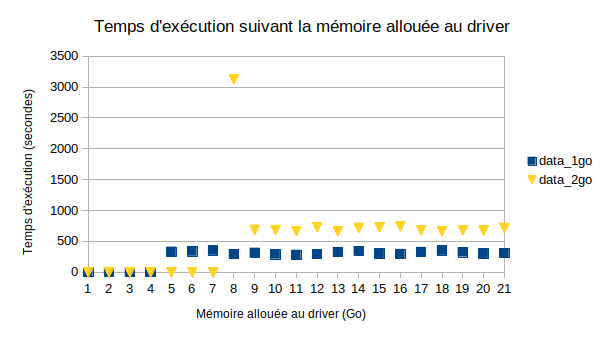
\includegraphics[width=1\linewidth]{illustrations/variant_driver_memory}
	\caption{Mesure des temps d'exécution de l'application Spark selon différentes tailles de mémoire allouées au \textit{driver} et pour deux ensembles de données différentes}
	\label{fig:variantdrivermemory}
\end{figure}

D'après la Figure 	\ref{fig:variantdrivermemory}, nous remarquons qu'à partir d'une taille mémoire allouée au driver, le temps écoulé durant l'exécution de l'application Spark est relativement stable. De plus, nous constatons qu'il faut prévoir une taille mémoire minimal pour assurer l'exécution de l'application Spark. Les tailles mémoire supérieures à cette valeur minimale affectent faiblement le temps d'exécution.  Cette valeur minimale dépend fortement de la quantité de données à analyser. Enfin, malgré que la machine sur laquelle nous lançons l'application Spark ne dispose que de $ 32 $ Go de RAM, le fait d'allouer au driver $ 35 $ Go, $ 40$ Go, $ 45 $ Go n'a pas généré une erreur lors de l'exécution.

\paragraph{Variant le mode local : local vs local[N]}~

local[*] Run Spark locally with as many worker threads as logical cores on your machine.
local [*] Exécutez Spark localement avec autant de threads de travail que de c\oe{}urs logiques sur votre ordinateur.

\paragraph{Notes concernant le mode local}~

Le mode local d'exécution d'une application Spark est typiquement utilisé pour tester le code sur une petite quantité de données dans un environnement local. Cependant, ce mode  ne fournit pas les avantages de l'environnement distribué. 

\subsection{Cluster Amazon EMR}

Nous avons utilisé l'infrastructure d'Amazon pour lancer la détection des anomalies. Ce sont les mêmes traitements lancés dans le mode local. Nous évaluons la détection en variant deux éléments. Dans un premier temps, nous varions la taille du cluster créé pour lancer la détection. Dans ce cas, nous utilisons différents nombre d'\textit{executors}. Pour le deuxième cas, nous fixons les caractéristiques du cluster et  nous choisissons différents ensembles de traceroutes. 
\paragraph{Variant la taille du cluster}


\subparagraph{Description de l'ensemble de données}

\begin{table}[H]
	\centering
	\begin{tabular}{|c|c|c|c|c|c|}
	\hline 
Id	& Taille  & Nb. de traceroutes & Nb.liens analysé & Id. msm& période \\ 
	\hline 
\end{tabular} 
\caption{text}
\label{key}
\end{table}



\subparagraph{Description des clusters}~

Le tableau \ref{clusters-description} décrit les clusters créés, il reprend le nom du cluster, le nombre d'instances formant le cluster en plus de l'instance représentant le \textit{driver}. 

\begin{table}[H]
	\centering
	\begin{tabular}{|c|c|c|}
	\hline 
\textbf{Nom du cluster}	&\textbf{Nombre d'instances}	&  \textbf{Types d'instances}   \\ 
	\hline 
C1	&   0 &  m4.large  \\ 
	\hline 
C2	&  &  \\ 
	\hline 
C3	&  &  \\ 
	\hline 
C4	&  &  \\ 
	\hline 
\end{tabular} 
\caption{}
\label{clusters-description}
\end{table}

Où x4.large a les caractéristiques suivantes : (vCPU : 2, Mém. (GiB) : 8, Stockage : EBS uniquement, Bande passante dédiée à EBS (Mbit/s) : 450, Performances réseau : Modéré).

\begin{comment}
DelayAnalysis-one-instance : C1
\end{comment}

\paragraph{Variant la taille de données}

\subparagraph{Description de l'ensemble de données}
\begin{table}[H]
	\centering
	\begin{tabular}{|c|c|c|c|c|c|}
		\hline 
		Id	& Taille  & Nb. de traceroutes & Nb.liens analysé & Id. msm& période \\ 
		\hline 
		&  &  &  & & \\ 
		\hline 
		&  &  &  & & \\ 
		\hline 
		&  &  &  & & \\ 
		\hline 
	\end{tabular} 
\caption{text}
\label{key}
\end{table}







\section{Conclusion}



%\chapter*{Conclusion}
%\addcontentsline{toc}{chapter}{Conclusion}
%\markboth{\textsl{Conclusion}}{\textsl{Conclusion}}}

%Quelques lignes pour finir...

%\appendix

%\chapter{Présentation du traceroute}

\paragraph{Les attributs } \label{annexe:traceroute-attributes}

\begin{figure}[H]
	\centering
	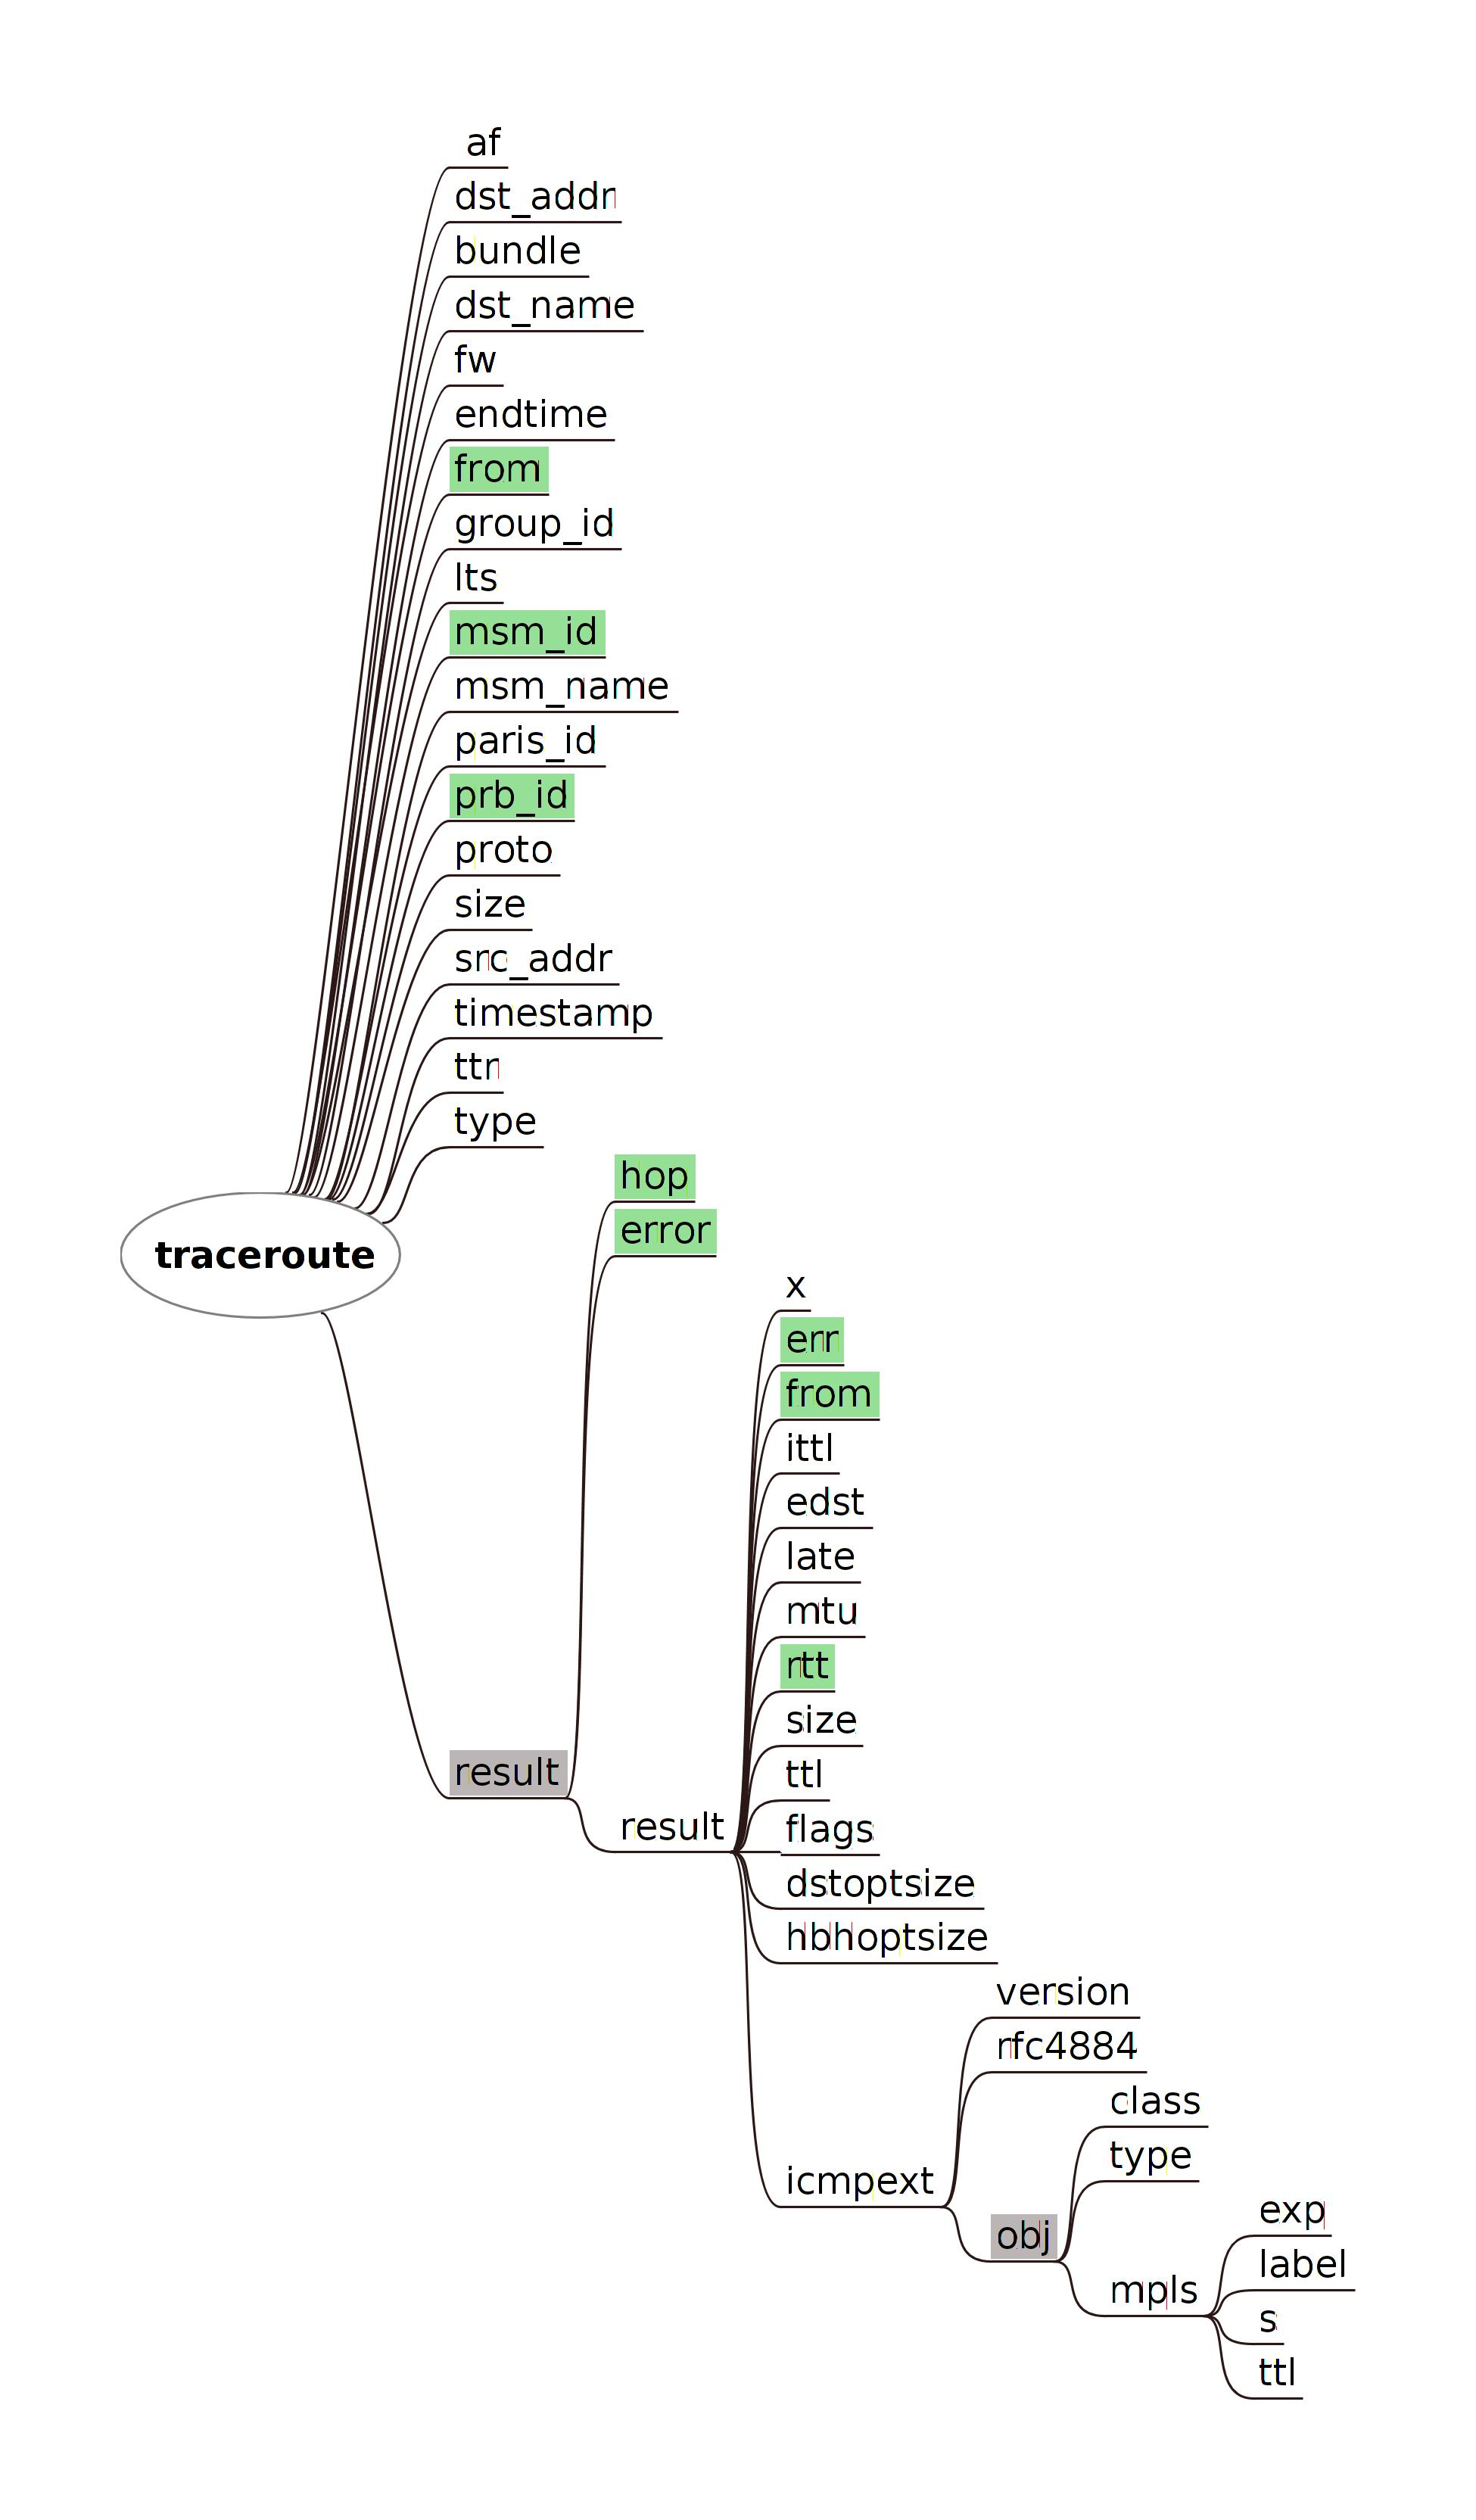
\includegraphics[width=0.7\linewidth]{illustrations/traceroute_attributes}
	\caption{Les attributs possibles dans le résultat d'une requête traceroute}
	\label{fig:traceroute_attributes}
\end{figure}


% Si vous utilisez (conseillé) BibTeX pour votre bibliographie :
\bibliographystyle{acm}
\bibliography{references}% si le fichier BibTeX est memoire.bib

\end{document}
%%% Local Variables: 
%%% mode: latex
%%% TeX-master: t
%%% TeX-PDF-mode: t
%%% End: 


\begin{landscape}
	\begin{table}
		\centering
		\begin{tabularx}{24cm}{ X X X XXX}
			
			
			
			MongoDB&DynamoDB &AWS (S3) &AWS ( Glue) &AWS ( Athena) &Apache Spark\\
			
			\textbf{Technologies}&&&&&\\
			
			%\textbf{collecte de données} &&&&&\\
			\textbf{Stockage} &&&&&\\
			\textbf{traitement}&&&&&\\
			\textbf{visualisation}&	  \LeftThumbsUp  flexible (schema-less database)
			
			\RightThumbsDown&&&&\\
			
		\end{tabularx}
		\caption{Récaputilatif des technologies Big Data expérimentées dans l'analyse des délais}
	\end{table}
\end{landscape}